\documentclass{book}
\usepackage[a4paper,top=2.5cm,bottom=2.5cm,left=2.5cm,right=2.5cm]{geometry}
\usepackage{makeidx}
\usepackage{natbib}
\usepackage{graphicx}
\usepackage{multicol}
\usepackage{float}
\usepackage{listings}
\usepackage{color}
\usepackage{ifthen}
\usepackage[table]{xcolor}
\usepackage{textcomp}
\usepackage{alltt}
\usepackage{ifpdf}
\ifpdf
\usepackage[pdftex,
            pagebackref=true,
            colorlinks=true,
            linkcolor=blue,
            unicode
           ]{hyperref}
\else
\usepackage[ps2pdf,
            pagebackref=true,
            colorlinks=true,
            linkcolor=blue,
            unicode
           ]{hyperref}
\usepackage{pspicture}
\fi
\usepackage[utf8]{inputenc}
\usepackage{mathptmx}
\usepackage[scaled=.90]{helvet}
\usepackage{courier}
\usepackage{sectsty}
\usepackage{amssymb}
\usepackage[titles]{tocloft}
\usepackage{doxygen}
\lstset{language=C++,inputencoding=utf8,basicstyle=\footnotesize,breaklines=true,breakatwhitespace=true,tabsize=4,numbers=left }
\makeindex
\setcounter{tocdepth}{3}
\renewcommand{\footrulewidth}{0.4pt}
\renewcommand{\familydefault}{\sfdefault}
\hfuzz=15pt
\setlength{\emergencystretch}{15pt}
\hbadness=750
\tolerance=750
\begin{document}
\hypersetup{pageanchor=false,citecolor=blue}
\begin{titlepage}
\vspace*{7cm}
\begin{center}
{\Large C\-Comp }\\
\vspace*{1cm}
{\large Generated by Doxygen 1.8.3.1}\\
\vspace*{0.5cm}
{\small Wed May 15 2013 06:43:47}\\
\end{center}
\end{titlepage}
\clearemptydoublepage
\pagenumbering{roman}
\tableofcontents
\clearemptydoublepage
\pagenumbering{arabic}
\hypersetup{pageanchor=true,citecolor=blue}
\chapter{University of Nevada, Reno $<$br/$>$$<$br/$>$ C\-S 660 -\/ Compilers}
\label{index}\hypertarget{index}{}\input{index}
\chapter{Hierarchical Index}
\section{Class Hierarchy}
This inheritance list is sorted roughly, but not completely, alphabetically\-:\begin{DoxyCompactList}
\item \contentsline{section}{A\-S\-T}{\pageref{classAST}}{}
\begin{DoxyCompactList}
\item \contentsline{section}{Ast\-Add\-Expr}{\pageref{classAstAddExpr}}{}
\item \contentsline{section}{Ast\-And\-Expr}{\pageref{classAstAndExpr}}{}
\item \contentsline{section}{Ast\-Arg\-Expr\-List}{\pageref{classAstArgExprList}}{}
\item \contentsline{section}{Ast\-Assign\-Expr}{\pageref{classAstAssignExpr}}{}
\item \contentsline{section}{Ast\-Assign\-Op}{\pageref{classAstAssignOp}}{}
\item \contentsline{section}{Ast\-Break}{\pageref{classAstBreak}}{}
\item \contentsline{section}{Ast\-Cast\-Expr}{\pageref{classAstCastExpr}}{}
\item \contentsline{section}{Ast\-Compound\-Stmt}{\pageref{classAstCompoundStmt}}{}
\item \contentsline{section}{Ast\-Conditional\-Expr}{\pageref{classAstConditionalExpr}}{}
\item \contentsline{section}{Ast\-Constant}{\pageref{classAstConstant}}{}
\item \contentsline{section}{Ast\-Constant\-Expr}{\pageref{classAstConstantExpr}}{}
\item \contentsline{section}{Ast\-Continue}{\pageref{classAstContinue}}{}
\item \contentsline{section}{Ast\-Declaration\-List}{\pageref{classAstDeclarationList}}{}
\item \contentsline{section}{Ast\-Do\-While}{\pageref{classAstDoWhile}}{}
\item \contentsline{section}{Ast\-Eq\-Expr}{\pageref{classAstEqExpr}}{}
\item \contentsline{section}{Ast\-Expression}{\pageref{classAstExpression}}{}
\item \contentsline{section}{Ast\-Expr\-Stmt}{\pageref{classAstExprStmt}}{}
\item \contentsline{section}{Ast\-For}{\pageref{classAstFor}}{}
\item \contentsline{section}{Ast\-Goto}{\pageref{classAstGoto}}{}
\item \contentsline{section}{Ast\-I\-D}{\pageref{classAstID}}{}
\item \contentsline{section}{Ast\-If\-Else}{\pageref{classAstIfElse}}{}
\item \contentsline{section}{Ast\-Iteration}{\pageref{classAstIteration}}{}
\item \contentsline{section}{Ast\-Jump}{\pageref{classAstJump}}{}
\item \contentsline{section}{Ast\-Labeled\-Stmt}{\pageref{classAstLabeledStmt}}{}
\item \contentsline{section}{Ast\-Logic\-And\-Expr}{\pageref{classAstLogicAndExpr}}{}
\item \contentsline{section}{Ast\-Logic\-Or\-Expr}{\pageref{classAstLogicOrExpr}}{}
\item \contentsline{section}{Ast\-Mult\-Expr}{\pageref{classAstMultExpr}}{}
\item \contentsline{section}{Ast\-Node\-Stub}{\pageref{classAstNodeStub}}{}
\item \contentsline{section}{Ast\-O\-R\-Expr}{\pageref{classAstORExpr}}{}
\item \contentsline{section}{Ast\-Postfix\-Expr}{\pageref{classAstPostfixExpr}}{}
\item \contentsline{section}{Ast\-Primary\-Expr}{\pageref{classAstPrimaryExpr}}{}
\item \contentsline{section}{Ast\-Rel\-Expr}{\pageref{classAstRelExpr}}{}
\item \contentsline{section}{Ast\-Return}{\pageref{classAstReturn}}{}
\item \contentsline{section}{Ast\-Selection}{\pageref{classAstSelection}}{}
\item \contentsline{section}{Ast\-Shift\-Expr}{\pageref{classAstShiftExpr}}{}
\item \contentsline{section}{Ast\-Statement}{\pageref{classAstStatement}}{}
\item \contentsline{section}{Ast\-Statement\-List}{\pageref{classAstStatementList}}{}
\item \contentsline{section}{Ast\-String}{\pageref{classAstString}}{}
\item \contentsline{section}{Ast\-Switch}{\pageref{classAstSwitch}}{}
\item \contentsline{section}{Ast\-Type\-Name}{\pageref{classAstTypeName}}{}
\item \contentsline{section}{Ast\-Unary\-Expr}{\pageref{classAstUnaryExpr}}{}
\item \contentsline{section}{Ast\-Unary\-Op}{\pageref{classAstUnaryOp}}{}
\item \contentsline{section}{Ast\-While}{\pageref{classAstWhile}}{}
\item \contentsline{section}{Ast\-X\-O\-R\-Expr}{\pageref{classAstXORExpr}}{}
\end{DoxyCompactList}
\item \contentsline{section}{A\-V\-L\-Tree$<$ Data\-Item $>$}{\pageref{classAVLTree}}{}
\item \contentsline{section}{C\-Compiler}{\pageref{classCCompiler}}{}
\item \contentsline{section}{Input\-Line}{\pageref{structInputLine}}{}
\item \contentsline{section}{A\-V\-L\-Tree$<$ Data\-Item $>$\-:\-:Node}{\pageref{structAVLTree_1_1Node}}{}
\item \contentsline{section}{Symbol\-Info}{\pageref{structSymbolInfo}}{}
\item \contentsline{section}{Sym\-Tab}{\pageref{classSymTab}}{}
\item \contentsline{section}{T\-A\-C\-\_\-\-Generator}{\pageref{classTAC__Generator}}{}
\item \contentsline{section}{Type}{\pageref{classType}}{}
\begin{DoxyCompactList}
\item \contentsline{section}{Array\-Type}{\pageref{classArrayType}}{}
\item \contentsline{section}{Enum\-Type}{\pageref{classEnumType}}{}
\item \contentsline{section}{Function\-Type}{\pageref{classFunctionType}}{}
\item \contentsline{section}{P\-O\-D\-Type}{\pageref{classPODType}}{}
\item \contentsline{section}{Pointer\-Type}{\pageref{classPointerType}}{}
\item \contentsline{section}{Struct\-Type}{\pageref{classStructType}}{}
\item \contentsline{section}{Typedef\-Type}{\pageref{classTypedefType}}{}
\item \contentsline{section}{Union\-Type}{\pageref{classUnionType}}{}
\end{DoxyCompactList}
\item \contentsline{section}{Visualizer}{\pageref{classVisualizer}}{}
\end{DoxyCompactList}

\chapter{Class Index}
\section{Class List}
Here are the classes, structs, unions and interfaces with brief descriptions\-:\begin{DoxyCompactList}
\item\contentsline{section}{\hyperlink{structAddress}{Address} \\*This struct describes the entire location information of a variable in the program including the memory location flag, the name of the register it is in (if it is in a register), and the memory offset location it is in (if it is also in memory) }{\pageref{structAddress}}{}
\item\contentsline{section}{\hyperlink{classAddressTable}{Address\-Table} }{\pageref{classAddressTable}}{}
\item\contentsline{section}{\hyperlink{classArrayType}{Array\-Type} }{\pageref{classArrayType}}{}
\item\contentsline{section}{\hyperlink{classAST}{A\-S\-T} \\*Abstract syntax tree node type }{\pageref{classAST}}{}
\item\contentsline{section}{\hyperlink{classAstAbstractDecl}{Ast\-Abstract\-Decl} }{\pageref{classAstAbstractDecl}}{}
\item\contentsline{section}{\hyperlink{classAstAddExpr}{Ast\-Add\-Expr} }{\pageref{classAstAddExpr}}{}
\item\contentsline{section}{\hyperlink{classAstAndExpr}{Ast\-And\-Expr} }{\pageref{classAstAndExpr}}{}
\item\contentsline{section}{\hyperlink{classAstArgExprList}{Ast\-Arg\-Expr\-List} }{\pageref{classAstArgExprList}}{}
\item\contentsline{section}{\hyperlink{classAstAssignExpr}{Ast\-Assign\-Expr} }{\pageref{classAstAssignExpr}}{}
\item\contentsline{section}{\hyperlink{classAstAssignOp}{Ast\-Assign\-Op} }{\pageref{classAstAssignOp}}{}
\item\contentsline{section}{\hyperlink{classAstBreak}{Ast\-Break} }{\pageref{classAstBreak}}{}
\item\contentsline{section}{\hyperlink{classAstCastExpr}{Ast\-Cast\-Expr} }{\pageref{classAstCastExpr}}{}
\item\contentsline{section}{\hyperlink{classAstCompoundStmt}{Ast\-Compound\-Stmt} }{\pageref{classAstCompoundStmt}}{}
\item\contentsline{section}{\hyperlink{classAstConditionalExpr}{Ast\-Conditional\-Expr} }{\pageref{classAstConditionalExpr}}{}
\item\contentsline{section}{\hyperlink{classAstConstant}{Ast\-Constant} }{\pageref{classAstConstant}}{}
\item\contentsline{section}{\hyperlink{classAstConstantExpr}{Ast\-Constant\-Expr} }{\pageref{classAstConstantExpr}}{}
\item\contentsline{section}{\hyperlink{classAstContinue}{Ast\-Continue} }{\pageref{classAstContinue}}{}
\item\contentsline{section}{\hyperlink{classAstDecl}{Ast\-Decl} }{\pageref{classAstDecl}}{}
\item\contentsline{section}{\hyperlink{classAstDeclarationList}{Ast\-Declaration\-List} }{\pageref{classAstDeclarationList}}{}
\item\contentsline{section}{\hyperlink{classAstDeclarator}{Ast\-Declarator} }{\pageref{classAstDeclarator}}{}
\item\contentsline{section}{\hyperlink{classAstDeclList}{Ast\-Decl\-List} }{\pageref{classAstDeclList}}{}
\item\contentsline{section}{\hyperlink{classAstDecSpeci}{Ast\-Dec\-Speci} }{\pageref{classAstDecSpeci}}{}
\item\contentsline{section}{\hyperlink{classAstDirectAbsDecl}{Ast\-Direct\-Abs\-Decl} }{\pageref{classAstDirectAbsDecl}}{}
\item\contentsline{section}{\hyperlink{classAstDirectDecl}{Ast\-Direct\-Decl} }{\pageref{classAstDirectDecl}}{}
\item\contentsline{section}{\hyperlink{classAstDoWhile}{Ast\-Do\-While} }{\pageref{classAstDoWhile}}{}
\item\contentsline{section}{\hyperlink{classAstEnumerator}{Ast\-Enumerator} }{\pageref{classAstEnumerator}}{}
\item\contentsline{section}{\hyperlink{classAstEnumList}{Ast\-Enum\-List} }{\pageref{classAstEnumList}}{}
\item\contentsline{section}{\hyperlink{classAstEqExpr}{Ast\-Eq\-Expr} }{\pageref{classAstEqExpr}}{}
\item\contentsline{section}{\hyperlink{classAstExpression}{Ast\-Expression} }{\pageref{classAstExpression}}{}
\item\contentsline{section}{\hyperlink{classAstExprStmt}{Ast\-Expr\-Stmt} }{\pageref{classAstExprStmt}}{}
\item\contentsline{section}{\hyperlink{classAstFor}{Ast\-For} }{\pageref{classAstFor}}{}
\item\contentsline{section}{\hyperlink{classAstFuncDef}{Ast\-Func\-Def} }{\pageref{classAstFuncDef}}{}
\item\contentsline{section}{\hyperlink{classAstGoto}{Ast\-Goto} }{\pageref{classAstGoto}}{}
\item\contentsline{section}{\hyperlink{classAstID}{Ast\-I\-D} }{\pageref{classAstID}}{}
\item\contentsline{section}{\hyperlink{classAstIDList}{Ast\-I\-D\-List} }{\pageref{classAstIDList}}{}
\item\contentsline{section}{\hyperlink{classAstIfElse}{Ast\-If\-Else} }{\pageref{classAstIfElse}}{}
\item\contentsline{section}{\hyperlink{classAstInitDeclarator}{Ast\-Init\-Declarator} }{\pageref{classAstInitDeclarator}}{}
\item\contentsline{section}{\hyperlink{classAstInitDeclList}{Ast\-Init\-Decl\-List} }{\pageref{classAstInitDeclList}}{}
\item\contentsline{section}{\hyperlink{classAstInitializer}{Ast\-Initializer} }{\pageref{classAstInitializer}}{}
\item\contentsline{section}{\hyperlink{classAstInitList}{Ast\-Init\-List} }{\pageref{classAstInitList}}{}
\item\contentsline{section}{\hyperlink{classAstIteration}{Ast\-Iteration} }{\pageref{classAstIteration}}{}
\item\contentsline{section}{\hyperlink{classAstJump}{Ast\-Jump} }{\pageref{classAstJump}}{}
\item\contentsline{section}{\hyperlink{classAstLabeledStmt}{Ast\-Labeled\-Stmt} }{\pageref{classAstLabeledStmt}}{}
\item\contentsline{section}{\hyperlink{classAstLogicAndExpr}{Ast\-Logic\-And\-Expr} }{\pageref{classAstLogicAndExpr}}{}
\item\contentsline{section}{\hyperlink{classAstLogicOrExpr}{Ast\-Logic\-Or\-Expr} }{\pageref{classAstLogicOrExpr}}{}
\item\contentsline{section}{\hyperlink{classAstMultExpr}{Ast\-Mult\-Expr} }{\pageref{classAstMultExpr}}{}
\item\contentsline{section}{\hyperlink{classAstORExpr}{Ast\-O\-R\-Expr} }{\pageref{classAstORExpr}}{}
\item\contentsline{section}{\hyperlink{classAstParamDec}{Ast\-Param\-Dec} }{\pageref{classAstParamDec}}{}
\item\contentsline{section}{\hyperlink{classAstParamList}{Ast\-Param\-List} }{\pageref{classAstParamList}}{}
\item\contentsline{section}{\hyperlink{classAstPointer}{Ast\-Pointer} }{\pageref{classAstPointer}}{}
\item\contentsline{section}{\hyperlink{classAstPostfixExpr}{Ast\-Postfix\-Expr} }{\pageref{classAstPostfixExpr}}{}
\item\contentsline{section}{\hyperlink{classAstPrimaryExpr}{Ast\-Primary\-Expr} }{\pageref{classAstPrimaryExpr}}{}
\item\contentsline{section}{\hyperlink{classAstRelExpr}{Ast\-Rel\-Expr} }{\pageref{classAstRelExpr}}{}
\item\contentsline{section}{\hyperlink{classAstReturn}{Ast\-Return} }{\pageref{classAstReturn}}{}
\item\contentsline{section}{\hyperlink{classAstSelection}{Ast\-Selection} }{\pageref{classAstSelection}}{}
\item\contentsline{section}{\hyperlink{classAstShiftExpr}{Ast\-Shift\-Expr} }{\pageref{classAstShiftExpr}}{}
\item\contentsline{section}{\hyperlink{classAstSpeciQualList}{Ast\-Speci\-Qual\-List} }{\pageref{classAstSpeciQualList}}{}
\item\contentsline{section}{\hyperlink{classAstStatement}{Ast\-Statement} }{\pageref{classAstStatement}}{}
\item\contentsline{section}{\hyperlink{classAstStatementList}{Ast\-Statement\-List} }{\pageref{classAstStatementList}}{}
\item\contentsline{section}{\hyperlink{classAstString}{Ast\-String} }{\pageref{classAstString}}{}
\item\contentsline{section}{\hyperlink{classAstStructDecl}{Ast\-Struct\-Decl} }{\pageref{classAstStructDecl}}{}
\item\contentsline{section}{\hyperlink{classAstStructDeclarator}{Ast\-Struct\-Declarator} }{\pageref{classAstStructDeclarator}}{}
\item\contentsline{section}{\hyperlink{classAstStructDeclatorList}{Ast\-Struct\-Declator\-List} }{\pageref{classAstStructDeclatorList}}{}
\item\contentsline{section}{\hyperlink{classAstStructDeclList}{Ast\-Struct\-Decl\-List} }{\pageref{classAstStructDeclList}}{}
\item\contentsline{section}{\hyperlink{classAstStructUniSpeci}{Ast\-Struct\-Uni\-Speci} }{\pageref{classAstStructUniSpeci}}{}
\item\contentsline{section}{\hyperlink{classAstSwitch}{Ast\-Switch} }{\pageref{classAstSwitch}}{}
\item\contentsline{section}{\hyperlink{classAstTrans}{Ast\-Trans} }{\pageref{classAstTrans}}{}
\item\contentsline{section}{\hyperlink{classAstTypeName}{Ast\-Type\-Name} }{\pageref{classAstTypeName}}{}
\item\contentsline{section}{\hyperlink{classAstTypeParamList}{Ast\-Type\-Param\-List} }{\pageref{classAstTypeParamList}}{}
\item\contentsline{section}{\hyperlink{classAstTypeQualList}{Ast\-Type\-Qual\-List} }{\pageref{classAstTypeQualList}}{}
\item\contentsline{section}{\hyperlink{classAstTypeSpeci}{Ast\-Type\-Speci} }{\pageref{classAstTypeSpeci}}{}
\item\contentsline{section}{\hyperlink{classAstUnaryExpr}{Ast\-Unary\-Expr} }{\pageref{classAstUnaryExpr}}{}
\item\contentsline{section}{\hyperlink{classAstUnaryOp}{Ast\-Unary\-Op} }{\pageref{classAstUnaryOp}}{}
\item\contentsline{section}{\hyperlink{classAstWhile}{Ast\-While} }{\pageref{classAstWhile}}{}
\item\contentsline{section}{\hyperlink{classAstXORExpr}{Ast\-X\-O\-R\-Expr} }{\pageref{classAstXORExpr}}{}
\item\contentsline{section}{\hyperlink{classAVLTree}{A\-V\-L\-Tree$<$ Data\-Item $>$} \\*An implementation of a balanced binary tree called an A\-V\-L tree }{\pageref{classAVLTree}}{}
\item\contentsline{section}{\hyperlink{classCCompiler}{C\-Compiler} \\*A minimalist C programming language compiler class }{\pageref{classCCompiler}}{}
\item\contentsline{section}{\hyperlink{classEnumSpecifier}{Enum\-Specifier} }{\pageref{classEnumSpecifier}}{}
\item\contentsline{section}{\hyperlink{classEnumType}{Enum\-Type} }{\pageref{classEnumType}}{}
\item\contentsline{section}{\hyperlink{classGoFPatterns_1_1Event}{Go\-F\-Patterns\-::\-Event$<$ Source\-Type, Event\-Arg\-Type $>$} }{\pageref{classGoFPatterns_1_1Event}}{}
\item\contentsline{section}{\hyperlink{structFunction}{Function} }{\pageref{structFunction}}{}
\item\contentsline{section}{\hyperlink{classFunctionTable}{Function\-Table} }{\pageref{classFunctionTable}}{}
\item\contentsline{section}{\hyperlink{classFunctionType}{Function\-Type} }{\pageref{classFunctionType}}{}
\item\contentsline{section}{\hyperlink{structInputLine}{Input\-Line} \\*A structure for buffering lines input code }{\pageref{structInputLine}}{}
\item\contentsline{section}{\hyperlink{structAVLTree_1_1Node}{A\-V\-L\-Tree$<$ Data\-Item $>$\-::\-Node} \\*A node which composes the Data\-Item template class with pointers to its children nodes in the A\-V\-L tree and the balance factor at the current node }{\pageref{structAVLTree_1_1Node}}{}
\item\contentsline{section}{\hyperlink{structParameter}{Parameter} }{\pageref{structParameter}}{}
\item\contentsline{section}{\hyperlink{classPODType}{P\-O\-D\-Type} }{\pageref{classPODType}}{}
\item\contentsline{section}{\hyperlink{classPointerType}{Pointer\-Type} }{\pageref{classPointerType}}{}
\item\contentsline{section}{\hyperlink{classRegAllocTable}{Reg\-Alloc\-Table} }{\pageref{classRegAllocTable}}{}
\item\contentsline{section}{\hyperlink{structRegister}{Register} }{\pageref{structRegister}}{}
\item\contentsline{section}{\hyperlink{classStructType}{Struct\-Type} }{\pageref{classStructType}}{}
\item\contentsline{section}{\hyperlink{classGoFPatterns_1_1Event_1_1SubscriberRecord}{Go\-F\-Patterns\-::\-Event$<$ Source\-Type, Event\-Arg\-Type $>$\-::\-Subscriber\-Record} \\*This inner class, for each Event\-Handler, stores the associated context information -\/ pointer }{\pageref{classGoFPatterns_1_1Event_1_1SubscriberRecord}}{}
\item\contentsline{section}{\hyperlink{structSymbolInfo}{Symbol\-Info} }{\pageref{structSymbolInfo}}{}
\item\contentsline{section}{\hyperlink{classSymTab}{Sym\-Tab} }{\pageref{classSymTab}}{}
\item\contentsline{section}{\hyperlink{classtac2mips}{tac2mips} }{\pageref{classtac2mips}}{}
\item\contentsline{section}{\hyperlink{classTAC__Generator}{T\-A\-C\-\_\-\-Generator} \\*A class for generating three address code }{\pageref{classTAC__Generator}}{}
\item\contentsline{section}{\hyperlink{classType}{Type} }{\pageref{classType}}{}
\item\contentsline{section}{\hyperlink{classTypedefType}{Typedef\-Type} }{\pageref{classTypedefType}}{}
\item\contentsline{section}{\hyperlink{classUnionType}{Union\-Type} }{\pageref{classUnionType}}{}
\item\contentsline{section}{\hyperlink{classVisualizer}{Visualizer} \\*A class for visualizing the generation of the \hyperlink{classAST}{A\-S\-T} }{\pageref{classVisualizer}}{}
\end{DoxyCompactList}

\chapter{File Index}
\section{File List}
Here is a list of all documented files with brief descriptions\-:\begin{DoxyCompactList}
\item\contentsline{section}{{\bfseries Ast.\-cpp} }{\pageref{Ast_8cpp}}{}
\item\contentsline{section}{{\bfseries Ast.\-h} }{\pageref{Ast_8h}}{}
\item\contentsline{section}{{\bfseries Avl\-Tree.\-h} }{\pageref{AvlTree_8h}}{}
\item\contentsline{section}{{\bfseries C\-Compiler.\-cpp} }{\pageref{CCompiler_8cpp}}{}
\item\contentsline{section}{{\bfseries C\-Compiler.\-h} }{\pageref{CCompiler_8h}}{}
\item\contentsline{section}{\hyperlink{CParser_8yy}{C\-Parser.\-yy} \\*N\-O\-T\-E\-: U\-S\-E T\-H\-E L\-I\-N\-K B\-E\-L\-O\-W T\-O V\-I\-E\-W T\-H\-E S\-O\-U\-R\-C\-E F\-O\-R T\-H\-I\-S F\-I\-L\-E, T\-H\-E G\-E\-N\-E\-R\-A\-T\-E\-D D\-O\-C\-U\-M\-E\-N\-T\-A\-T\-I\-O\-N I\-S N\-O\-T V\-A\-L\-I\-D S\-I\-N\-C\-E D\-O\-X\-Y\-G\-E\-N C\-A\-N\-N\-O\-T P\-R\-O\-P\-E\-R\-L\-Y P\-A\-R\-S\-E B\-I\-S\-O\-N F\-I\-L\-E\-S! }{\pageref{CParser_8yy}}{}
\item\contentsline{section}{\hyperlink{CScanner_8ll}{C\-Scanner.\-ll} \\*N\-O\-T\-E\-: U\-S\-E T\-H\-E L\-I\-N\-K B\-E\-L\-O\-W T\-O V\-I\-E\-W T\-H\-E S\-O\-U\-R\-C\-E F\-O\-R T\-H\-I\-S F\-I\-L\-E, T\-H\-E G\-E\-N\-E\-R\-A\-T\-E\-D D\-O\-C\-U\-M\-E\-N\-T\-A\-T\-I\-O\-N I\-S N\-O\-T V\-A\-L\-I\-D S\-I\-N\-C\-E D\-O\-X\-Y\-G\-E\-N C\-A\-N\-N\-O\-T P\-R\-O\-P\-E\-R\-L\-Y P\-A\-R\-S\-E F\-L\-E\-X F\-I\-L\-E\-S! }{\pageref{CScanner_8ll}}{}
\item\contentsline{section}{\hyperlink{main_8cpp}{main.\-cpp} \\*This file serves as an entry point to the compiler }{\pageref{main_8cpp}}{}
\item\contentsline{section}{\hyperlink{Platform_8h}{Platform.\-h} \\*This file simply lists the size in bytes of the base data types }{\pageref{Platform_8h}}{}
\item\contentsline{section}{{\bfseries Sym\-Tab.\-cpp} }{\pageref{SymTab_8cpp}}{}
\item\contentsline{section}{{\bfseries Sym\-Tab.\-h} }{\pageref{SymTab_8h}}{}
\item\contentsline{section}{{\bfseries T\-A\-C\-\_\-\-Generator.\-cpp} }{\pageref{TAC__Generator_8cpp}}{}
\item\contentsline{section}{{\bfseries T\-A\-C\-\_\-\-Generator.\-h} }{\pageref{TAC__Generator_8h}}{}
\item\contentsline{section}{{\bfseries Type.\-cpp} }{\pageref{Type_8cpp}}{}
\item\contentsline{section}{{\bfseries Type.\-h} }{\pageref{Type_8h}}{}
\item\contentsline{section}{{\bfseries Visualizer.\-cpp} }{\pageref{Visualizer_8cpp}}{}
\item\contentsline{section}{{\bfseries Visualizer.\-h} }{\pageref{Visualizer_8h}}{}
\item\contentsline{section}{mips/{\bfseries Address\-Table.\-cpp} }{\pageref{AddressTable_8cpp}}{}
\item\contentsline{section}{mips/{\bfseries Address\-Table.\-h} }{\pageref{AddressTable_8h}}{}
\item\contentsline{section}{mips/{\bfseries Address\-Test.\-cpp} }{\pageref{AddressTest_8cpp}}{}
\item\contentsline{section}{mips/{\bfseries Event.\-h} }{\pageref{Event_8h}}{}
\item\contentsline{section}{mips/{\bfseries Function\-Table.\-cpp} }{\pageref{FunctionTable_8cpp}}{}
\item\contentsline{section}{mips/{\bfseries Function\-Table.\-h} }{\pageref{FunctionTable_8h}}{}
\item\contentsline{section}{mips/{\bfseries main.\-cpp} }{\pageref{mips_2main_8cpp}}{}
\item\contentsline{section}{mips/{\bfseries Reg\-Alloc\-Table.\-cpp} }{\pageref{RegAllocTable_8cpp}}{}
\item\contentsline{section}{mips/{\bfseries Reg\-Alloc\-Table.\-h} }{\pageref{RegAllocTable_8h}}{}
\item\contentsline{section}{mips/{\bfseries Spill\-Test.\-cpp} }{\pageref{SpillTest_8cpp}}{}
\item\contentsline{section}{mips/{\bfseries tac2mips.\-cpp} }{\pageref{tac2mips_8cpp}}{}
\item\contentsline{section}{mips/{\bfseries tac2mips.\-h} }{\pageref{tac2mips_8h}}{}
\item\contentsline{section}{mips/{\bfseries T\-A\-C\-\_\-\-Parser.\-yy} }{\pageref{TAC__Parser_8yy}}{}
\item\contentsline{section}{mips/{\bfseries T\-A\-C\-\_\-\-Scanner.\-ll} }{\pageref{TAC__Scanner_8ll}}{}
\item\contentsline{section}{tests/{\bfseries test1.\-c} }{\pageref{test1_8c}}{}
\item\contentsline{section}{tests/{\bfseries test2.\-c} }{\pageref{test2_8c}}{}
\item\contentsline{section}{tests/{\bfseries test2a.\-c} }{\pageref{test2a_8c}}{}
\item\contentsline{section}{tests/{\bfseries test3.\-c} }{\pageref{test3_8c}}{}
\item\contentsline{section}{tests/{\bfseries test4.\-c} }{\pageref{test4_8c}}{}
\item\contentsline{section}{tests/{\bfseries test5.\-c} }{\pageref{test5_8c}}{}
\item\contentsline{section}{tests/{\bfseries test6.\-c} }{\pageref{test6_8c}}{}
\item\contentsline{section}{tests/{\bfseries test7.\-c} }{\pageref{test7_8c}}{}
\item\contentsline{section}{tests/{\bfseries test8.\-c} }{\pageref{test8_8c}}{}
\end{DoxyCompactList}

\chapter{Class Documentation}
\input{structAddress}
\input{classAddressTable}
\hypertarget{classArrayType}{\section{Array\-Type Class Reference}
\label{classArrayType}\index{Array\-Type@{Array\-Type}}
}
Inheritance diagram for Array\-Type\-:\begin{figure}[H]
\begin{center}
\leavevmode
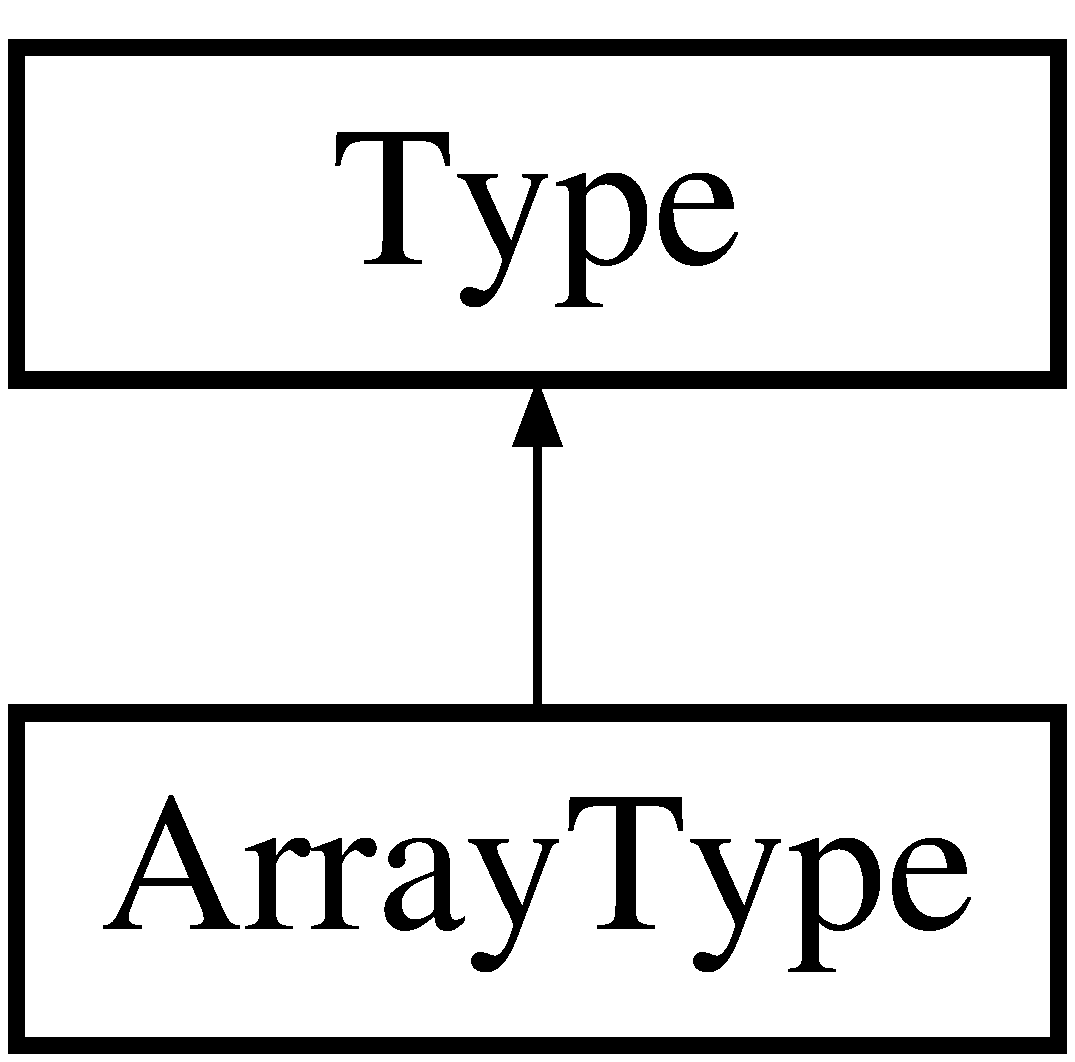
\includegraphics[height=12.000000cm]{classArrayType}
\end{center}
\end{figure}
\subsection*{Public Types}
\begin{DoxyCompactItemize}
\item 
enum {\bfseries Derived\-Type} \{ \\*
{\bfseries B\-A\-S\-E}, 
{\bfseries P\-O\-D\-T\-Y\-P\-E}, 
{\bfseries T\-Y\-P\-E\-D\-E\-F\-T\-Y\-P\-E}, 
{\bfseries E\-N\-U\-M\-T\-Y\-P\-E}, 
\\*
{\bfseries A\-R\-R\-A\-Y\-T\-Y\-P\-E}, 
{\bfseries S\-T\-R\-U\-C\-T\-T\-Y\-P\-E}, 
{\bfseries U\-N\-I\-O\-N\-T\-Y\-P\-E}, 
{\bfseries F\-U\-N\-C\-T\-I\-O\-N\-T\-Y\-P\-E}, 
\\*
{\bfseries P\-O\-I\-N\-T\-E\-R\-T\-Y\-P\-E}, 
{\bfseries B\-A\-S\-E}, 
{\bfseries P\-O\-D\-T\-Y\-P\-E}, 
{\bfseries T\-Y\-P\-E\-D\-E\-F\-T\-Y\-P\-E}, 
\\*
{\bfseries E\-N\-U\-M\-T\-Y\-P\-E}, 
{\bfseries A\-R\-R\-A\-Y\-T\-Y\-P\-E}, 
{\bfseries S\-T\-R\-U\-C\-T\-T\-Y\-P\-E}, 
{\bfseries U\-N\-I\-O\-N\-T\-Y\-P\-E}, 
\\*
{\bfseries F\-U\-N\-C\-T\-I\-O\-N\-T\-Y\-P\-E}, 
{\bfseries P\-O\-I\-N\-T\-E\-R\-T\-Y\-P\-E}, 
{\bfseries B\-A\-S\-E}, 
{\bfseries P\-O\-D\-T\-Y\-P\-E}, 
\\*
{\bfseries T\-Y\-P\-E\-D\-E\-F\-T\-Y\-P\-E}, 
{\bfseries E\-N\-U\-M\-T\-Y\-P\-E}, 
{\bfseries A\-R\-R\-A\-Y\-T\-Y\-P\-E}, 
{\bfseries S\-T\-R\-U\-C\-T\-T\-Y\-P\-E}, 
\\*
{\bfseries U\-N\-I\-O\-N\-T\-Y\-P\-E}, 
{\bfseries F\-U\-N\-C\-T\-I\-O\-N\-T\-Y\-P\-E}, 
{\bfseries P\-O\-I\-N\-T\-E\-R\-T\-Y\-P\-E}, 
{\bfseries B\-A\-S\-E}, 
\\*
{\bfseries P\-O\-D\-T\-Y\-P\-E}, 
{\bfseries T\-Y\-P\-E\-D\-E\-F\-T\-Y\-P\-E}, 
{\bfseries E\-N\-U\-M\-T\-Y\-P\-E}, 
{\bfseries A\-R\-R\-A\-Y\-T\-Y\-P\-E}, 
\\*
{\bfseries S\-T\-R\-U\-C\-T\-T\-Y\-P\-E}, 
{\bfseries U\-N\-I\-O\-N\-T\-Y\-P\-E}, 
{\bfseries F\-U\-N\-C\-T\-I\-O\-N\-T\-Y\-P\-E}, 
{\bfseries P\-O\-I\-N\-T\-E\-R\-T\-Y\-P\-E}, 
\\*
{\bfseries B\-A\-S\-E}, 
{\bfseries P\-O\-D\-T\-Y\-P\-E}, 
{\bfseries T\-Y\-P\-E\-D\-E\-F\-T\-Y\-P\-E}, 
{\bfseries E\-N\-U\-M\-T\-Y\-P\-E}, 
\\*
{\bfseries A\-R\-R\-A\-Y\-T\-Y\-P\-E}, 
{\bfseries S\-T\-R\-U\-C\-T\-T\-Y\-P\-E}, 
{\bfseries U\-N\-I\-O\-N\-T\-Y\-P\-E}, 
{\bfseries F\-U\-N\-C\-T\-I\-O\-N\-T\-Y\-P\-E}, 
\\*
{\bfseries P\-O\-I\-N\-T\-E\-R\-T\-Y\-P\-E}, 
{\bfseries B\-A\-S\-E}, 
{\bfseries P\-O\-D\-T\-Y\-P\-E}, 
{\bfseries T\-Y\-P\-E\-D\-E\-F\-T\-Y\-P\-E}, 
\\*
{\bfseries E\-N\-U\-M\-T\-Y\-P\-E}, 
{\bfseries A\-R\-R\-A\-Y\-T\-Y\-P\-E}, 
{\bfseries S\-T\-R\-U\-C\-T\-T\-Y\-P\-E}, 
{\bfseries U\-N\-I\-O\-N\-T\-Y\-P\-E}, 
\\*
{\bfseries F\-U\-N\-C\-T\-I\-O\-N\-T\-Y\-P\-E}, 
{\bfseries P\-O\-I\-N\-T\-E\-R\-T\-Y\-P\-E}, 
{\bfseries B\-A\-S\-E}, 
{\bfseries P\-O\-D\-T\-Y\-P\-E}, 
\\*
{\bfseries T\-Y\-P\-E\-D\-E\-F\-T\-Y\-P\-E}, 
{\bfseries E\-N\-U\-M\-T\-Y\-P\-E}, 
{\bfseries A\-R\-R\-A\-Y\-T\-Y\-P\-E}, 
{\bfseries S\-T\-R\-U\-C\-T\-T\-Y\-P\-E}, 
\\*
{\bfseries U\-N\-I\-O\-N\-T\-Y\-P\-E}, 
{\bfseries F\-U\-N\-C\-T\-I\-O\-N\-T\-Y\-P\-E}, 
{\bfseries P\-O\-I\-N\-T\-E\-R\-T\-Y\-P\-E}, 
{\bfseries B\-A\-S\-E}, 
\\*
{\bfseries P\-O\-D\-T\-Y\-P\-E}, 
{\bfseries T\-Y\-P\-E\-D\-E\-F\-T\-Y\-P\-E}, 
{\bfseries E\-N\-U\-M\-T\-Y\-P\-E}, 
{\bfseries A\-R\-R\-A\-Y\-T\-Y\-P\-E}, 
\\*
{\bfseries S\-T\-R\-U\-C\-T\-T\-Y\-P\-E}, 
{\bfseries U\-N\-I\-O\-N\-T\-Y\-P\-E}, 
{\bfseries F\-U\-N\-C\-T\-I\-O\-N\-T\-Y\-P\-E}, 
{\bfseries P\-O\-I\-N\-T\-E\-R\-T\-Y\-P\-E}, 
\\*
{\bfseries B\-A\-S\-E}, 
{\bfseries P\-O\-D\-T\-Y\-P\-E}, 
{\bfseries T\-Y\-P\-E\-D\-E\-F\-T\-Y\-P\-E}, 
{\bfseries E\-N\-U\-M\-T\-Y\-P\-E}, 
\\*
{\bfseries A\-R\-R\-A\-Y\-T\-Y\-P\-E}, 
{\bfseries S\-T\-R\-U\-C\-T\-T\-Y\-P\-E}, 
{\bfseries U\-N\-I\-O\-N\-T\-Y\-P\-E}, 
{\bfseries F\-U\-N\-C\-T\-I\-O\-N\-T\-Y\-P\-E}, 
\\*
{\bfseries P\-O\-I\-N\-T\-E\-R\-T\-Y\-P\-E}, 
{\bfseries B\-A\-S\-E}, 
{\bfseries P\-O\-D\-T\-Y\-P\-E}, 
{\bfseries T\-Y\-P\-E\-D\-E\-F\-T\-Y\-P\-E}, 
\\*
{\bfseries E\-N\-U\-M\-T\-Y\-P\-E}, 
{\bfseries A\-R\-R\-A\-Y\-T\-Y\-P\-E}, 
{\bfseries S\-T\-R\-U\-C\-T\-T\-Y\-P\-E}, 
{\bfseries U\-N\-I\-O\-N\-T\-Y\-P\-E}, 
\\*
{\bfseries F\-U\-N\-C\-T\-I\-O\-N\-T\-Y\-P\-E}, 
{\bfseries P\-O\-I\-N\-T\-E\-R\-T\-Y\-P\-E}, 
{\bfseries B\-A\-S\-E}, 
{\bfseries P\-O\-D\-T\-Y\-P\-E}, 
\\*
{\bfseries T\-Y\-P\-E\-D\-E\-F\-T\-Y\-P\-E}, 
{\bfseries E\-N\-U\-M\-T\-Y\-P\-E}, 
{\bfseries A\-R\-R\-A\-Y\-T\-Y\-P\-E}, 
{\bfseries S\-T\-R\-U\-C\-T\-T\-Y\-P\-E}, 
\\*
{\bfseries U\-N\-I\-O\-N\-T\-Y\-P\-E}, 
{\bfseries F\-U\-N\-C\-T\-I\-O\-N\-T\-Y\-P\-E}, 
{\bfseries P\-O\-I\-N\-T\-E\-R\-T\-Y\-P\-E}, 
{\bfseries B\-A\-S\-E}, 
\\*
{\bfseries P\-O\-D\-T\-Y\-P\-E}, 
{\bfseries T\-Y\-P\-E\-D\-E\-F\-T\-Y\-P\-E}, 
{\bfseries E\-N\-U\-M\-T\-Y\-P\-E}, 
{\bfseries A\-R\-R\-A\-Y\-T\-Y\-P\-E}, 
\\*
{\bfseries S\-T\-R\-U\-C\-T\-T\-Y\-P\-E}, 
{\bfseries U\-N\-I\-O\-N\-T\-Y\-P\-E}, 
{\bfseries F\-U\-N\-C\-T\-I\-O\-N\-T\-Y\-P\-E}, 
{\bfseries P\-O\-I\-N\-T\-E\-R\-T\-Y\-P\-E}, 
\\*
{\bfseries B\-A\-S\-E}, 
{\bfseries P\-O\-D\-T\-Y\-P\-E}, 
{\bfseries T\-Y\-P\-E\-D\-E\-F\-T\-Y\-P\-E}, 
{\bfseries E\-N\-U\-M\-T\-Y\-P\-E}, 
\\*
{\bfseries A\-R\-R\-A\-Y\-T\-Y\-P\-E}, 
{\bfseries S\-T\-R\-U\-C\-T\-T\-Y\-P\-E}, 
{\bfseries U\-N\-I\-O\-N\-T\-Y\-P\-E}, 
{\bfseries F\-U\-N\-C\-T\-I\-O\-N\-T\-Y\-P\-E}, 
\\*
{\bfseries P\-O\-I\-N\-T\-E\-R\-T\-Y\-P\-E}
 \}
\item 
enum {\bfseries Derived\-Type} \{ \\*
{\bfseries B\-A\-S\-E}, 
{\bfseries P\-O\-D\-T\-Y\-P\-E}, 
{\bfseries T\-Y\-P\-E\-D\-E\-F\-T\-Y\-P\-E}, 
{\bfseries E\-N\-U\-M\-T\-Y\-P\-E}, 
\\*
{\bfseries A\-R\-R\-A\-Y\-T\-Y\-P\-E}, 
{\bfseries S\-T\-R\-U\-C\-T\-T\-Y\-P\-E}, 
{\bfseries U\-N\-I\-O\-N\-T\-Y\-P\-E}, 
{\bfseries F\-U\-N\-C\-T\-I\-O\-N\-T\-Y\-P\-E}, 
\\*
{\bfseries P\-O\-I\-N\-T\-E\-R\-T\-Y\-P\-E}, 
{\bfseries B\-A\-S\-E}, 
{\bfseries P\-O\-D\-T\-Y\-P\-E}, 
{\bfseries T\-Y\-P\-E\-D\-E\-F\-T\-Y\-P\-E}, 
\\*
{\bfseries E\-N\-U\-M\-T\-Y\-P\-E}, 
{\bfseries A\-R\-R\-A\-Y\-T\-Y\-P\-E}, 
{\bfseries S\-T\-R\-U\-C\-T\-T\-Y\-P\-E}, 
{\bfseries U\-N\-I\-O\-N\-T\-Y\-P\-E}, 
\\*
{\bfseries F\-U\-N\-C\-T\-I\-O\-N\-T\-Y\-P\-E}, 
{\bfseries P\-O\-I\-N\-T\-E\-R\-T\-Y\-P\-E}, 
{\bfseries B\-A\-S\-E}, 
{\bfseries P\-O\-D\-T\-Y\-P\-E}, 
\\*
{\bfseries T\-Y\-P\-E\-D\-E\-F\-T\-Y\-P\-E}, 
{\bfseries E\-N\-U\-M\-T\-Y\-P\-E}, 
{\bfseries A\-R\-R\-A\-Y\-T\-Y\-P\-E}, 
{\bfseries S\-T\-R\-U\-C\-T\-T\-Y\-P\-E}, 
\\*
{\bfseries U\-N\-I\-O\-N\-T\-Y\-P\-E}, 
{\bfseries F\-U\-N\-C\-T\-I\-O\-N\-T\-Y\-P\-E}, 
{\bfseries P\-O\-I\-N\-T\-E\-R\-T\-Y\-P\-E}, 
{\bfseries B\-A\-S\-E}, 
\\*
{\bfseries P\-O\-D\-T\-Y\-P\-E}, 
{\bfseries T\-Y\-P\-E\-D\-E\-F\-T\-Y\-P\-E}, 
{\bfseries E\-N\-U\-M\-T\-Y\-P\-E}, 
{\bfseries A\-R\-R\-A\-Y\-T\-Y\-P\-E}, 
\\*
{\bfseries S\-T\-R\-U\-C\-T\-T\-Y\-P\-E}, 
{\bfseries U\-N\-I\-O\-N\-T\-Y\-P\-E}, 
{\bfseries F\-U\-N\-C\-T\-I\-O\-N\-T\-Y\-P\-E}, 
{\bfseries P\-O\-I\-N\-T\-E\-R\-T\-Y\-P\-E}, 
\\*
{\bfseries B\-A\-S\-E}, 
{\bfseries P\-O\-D\-T\-Y\-P\-E}, 
{\bfseries T\-Y\-P\-E\-D\-E\-F\-T\-Y\-P\-E}, 
{\bfseries E\-N\-U\-M\-T\-Y\-P\-E}, 
\\*
{\bfseries A\-R\-R\-A\-Y\-T\-Y\-P\-E}, 
{\bfseries S\-T\-R\-U\-C\-T\-T\-Y\-P\-E}, 
{\bfseries U\-N\-I\-O\-N\-T\-Y\-P\-E}, 
{\bfseries F\-U\-N\-C\-T\-I\-O\-N\-T\-Y\-P\-E}, 
\\*
{\bfseries P\-O\-I\-N\-T\-E\-R\-T\-Y\-P\-E}, 
{\bfseries B\-A\-S\-E}, 
{\bfseries P\-O\-D\-T\-Y\-P\-E}, 
{\bfseries T\-Y\-P\-E\-D\-E\-F\-T\-Y\-P\-E}, 
\\*
{\bfseries E\-N\-U\-M\-T\-Y\-P\-E}, 
{\bfseries A\-R\-R\-A\-Y\-T\-Y\-P\-E}, 
{\bfseries S\-T\-R\-U\-C\-T\-T\-Y\-P\-E}, 
{\bfseries U\-N\-I\-O\-N\-T\-Y\-P\-E}, 
\\*
{\bfseries F\-U\-N\-C\-T\-I\-O\-N\-T\-Y\-P\-E}, 
{\bfseries P\-O\-I\-N\-T\-E\-R\-T\-Y\-P\-E}, 
{\bfseries B\-A\-S\-E}, 
{\bfseries P\-O\-D\-T\-Y\-P\-E}, 
\\*
{\bfseries T\-Y\-P\-E\-D\-E\-F\-T\-Y\-P\-E}, 
{\bfseries E\-N\-U\-M\-T\-Y\-P\-E}, 
{\bfseries A\-R\-R\-A\-Y\-T\-Y\-P\-E}, 
{\bfseries S\-T\-R\-U\-C\-T\-T\-Y\-P\-E}, 
\\*
{\bfseries U\-N\-I\-O\-N\-T\-Y\-P\-E}, 
{\bfseries F\-U\-N\-C\-T\-I\-O\-N\-T\-Y\-P\-E}, 
{\bfseries P\-O\-I\-N\-T\-E\-R\-T\-Y\-P\-E}, 
{\bfseries B\-A\-S\-E}, 
\\*
{\bfseries P\-O\-D\-T\-Y\-P\-E}, 
{\bfseries T\-Y\-P\-E\-D\-E\-F\-T\-Y\-P\-E}, 
{\bfseries E\-N\-U\-M\-T\-Y\-P\-E}, 
{\bfseries A\-R\-R\-A\-Y\-T\-Y\-P\-E}, 
\\*
{\bfseries S\-T\-R\-U\-C\-T\-T\-Y\-P\-E}, 
{\bfseries U\-N\-I\-O\-N\-T\-Y\-P\-E}, 
{\bfseries F\-U\-N\-C\-T\-I\-O\-N\-T\-Y\-P\-E}, 
{\bfseries P\-O\-I\-N\-T\-E\-R\-T\-Y\-P\-E}, 
\\*
{\bfseries B\-A\-S\-E}, 
{\bfseries P\-O\-D\-T\-Y\-P\-E}, 
{\bfseries T\-Y\-P\-E\-D\-E\-F\-T\-Y\-P\-E}, 
{\bfseries E\-N\-U\-M\-T\-Y\-P\-E}, 
\\*
{\bfseries A\-R\-R\-A\-Y\-T\-Y\-P\-E}, 
{\bfseries S\-T\-R\-U\-C\-T\-T\-Y\-P\-E}, 
{\bfseries U\-N\-I\-O\-N\-T\-Y\-P\-E}, 
{\bfseries F\-U\-N\-C\-T\-I\-O\-N\-T\-Y\-P\-E}, 
\\*
{\bfseries P\-O\-I\-N\-T\-E\-R\-T\-Y\-P\-E}, 
{\bfseries B\-A\-S\-E}, 
{\bfseries P\-O\-D\-T\-Y\-P\-E}, 
{\bfseries T\-Y\-P\-E\-D\-E\-F\-T\-Y\-P\-E}, 
\\*
{\bfseries E\-N\-U\-M\-T\-Y\-P\-E}, 
{\bfseries A\-R\-R\-A\-Y\-T\-Y\-P\-E}, 
{\bfseries S\-T\-R\-U\-C\-T\-T\-Y\-P\-E}, 
{\bfseries U\-N\-I\-O\-N\-T\-Y\-P\-E}, 
\\*
{\bfseries F\-U\-N\-C\-T\-I\-O\-N\-T\-Y\-P\-E}, 
{\bfseries P\-O\-I\-N\-T\-E\-R\-T\-Y\-P\-E}, 
{\bfseries B\-A\-S\-E}, 
{\bfseries P\-O\-D\-T\-Y\-P\-E}, 
\\*
{\bfseries T\-Y\-P\-E\-D\-E\-F\-T\-Y\-P\-E}, 
{\bfseries E\-N\-U\-M\-T\-Y\-P\-E}, 
{\bfseries A\-R\-R\-A\-Y\-T\-Y\-P\-E}, 
{\bfseries S\-T\-R\-U\-C\-T\-T\-Y\-P\-E}, 
\\*
{\bfseries U\-N\-I\-O\-N\-T\-Y\-P\-E}, 
{\bfseries F\-U\-N\-C\-T\-I\-O\-N\-T\-Y\-P\-E}, 
{\bfseries P\-O\-I\-N\-T\-E\-R\-T\-Y\-P\-E}, 
{\bfseries B\-A\-S\-E}, 
\\*
{\bfseries P\-O\-D\-T\-Y\-P\-E}, 
{\bfseries T\-Y\-P\-E\-D\-E\-F\-T\-Y\-P\-E}, 
{\bfseries E\-N\-U\-M\-T\-Y\-P\-E}, 
{\bfseries A\-R\-R\-A\-Y\-T\-Y\-P\-E}, 
\\*
{\bfseries S\-T\-R\-U\-C\-T\-T\-Y\-P\-E}, 
{\bfseries U\-N\-I\-O\-N\-T\-Y\-P\-E}, 
{\bfseries F\-U\-N\-C\-T\-I\-O\-N\-T\-Y\-P\-E}, 
{\bfseries P\-O\-I\-N\-T\-E\-R\-T\-Y\-P\-E}, 
\\*
{\bfseries B\-A\-S\-E}, 
{\bfseries P\-O\-D\-T\-Y\-P\-E}, 
{\bfseries T\-Y\-P\-E\-D\-E\-F\-T\-Y\-P\-E}, 
{\bfseries E\-N\-U\-M\-T\-Y\-P\-E}, 
\\*
{\bfseries A\-R\-R\-A\-Y\-T\-Y\-P\-E}, 
{\bfseries S\-T\-R\-U\-C\-T\-T\-Y\-P\-E}, 
{\bfseries U\-N\-I\-O\-N\-T\-Y\-P\-E}, 
{\bfseries F\-U\-N\-C\-T\-I\-O\-N\-T\-Y\-P\-E}, 
\\*
{\bfseries P\-O\-I\-N\-T\-E\-R\-T\-Y\-P\-E}
 \}
\item 
enum {\bfseries Derived\-Type} \{ \\*
{\bfseries B\-A\-S\-E}, 
{\bfseries P\-O\-D\-T\-Y\-P\-E}, 
{\bfseries T\-Y\-P\-E\-D\-E\-F\-T\-Y\-P\-E}, 
{\bfseries E\-N\-U\-M\-T\-Y\-P\-E}, 
\\*
{\bfseries A\-R\-R\-A\-Y\-T\-Y\-P\-E}, 
{\bfseries S\-T\-R\-U\-C\-T\-T\-Y\-P\-E}, 
{\bfseries U\-N\-I\-O\-N\-T\-Y\-P\-E}, 
{\bfseries F\-U\-N\-C\-T\-I\-O\-N\-T\-Y\-P\-E}, 
\\*
{\bfseries P\-O\-I\-N\-T\-E\-R\-T\-Y\-P\-E}, 
{\bfseries B\-A\-S\-E}, 
{\bfseries P\-O\-D\-T\-Y\-P\-E}, 
{\bfseries T\-Y\-P\-E\-D\-E\-F\-T\-Y\-P\-E}, 
\\*
{\bfseries E\-N\-U\-M\-T\-Y\-P\-E}, 
{\bfseries A\-R\-R\-A\-Y\-T\-Y\-P\-E}, 
{\bfseries S\-T\-R\-U\-C\-T\-T\-Y\-P\-E}, 
{\bfseries U\-N\-I\-O\-N\-T\-Y\-P\-E}, 
\\*
{\bfseries F\-U\-N\-C\-T\-I\-O\-N\-T\-Y\-P\-E}, 
{\bfseries P\-O\-I\-N\-T\-E\-R\-T\-Y\-P\-E}, 
{\bfseries B\-A\-S\-E}, 
{\bfseries P\-O\-D\-T\-Y\-P\-E}, 
\\*
{\bfseries T\-Y\-P\-E\-D\-E\-F\-T\-Y\-P\-E}, 
{\bfseries E\-N\-U\-M\-T\-Y\-P\-E}, 
{\bfseries A\-R\-R\-A\-Y\-T\-Y\-P\-E}, 
{\bfseries S\-T\-R\-U\-C\-T\-T\-Y\-P\-E}, 
\\*
{\bfseries U\-N\-I\-O\-N\-T\-Y\-P\-E}, 
{\bfseries F\-U\-N\-C\-T\-I\-O\-N\-T\-Y\-P\-E}, 
{\bfseries P\-O\-I\-N\-T\-E\-R\-T\-Y\-P\-E}, 
{\bfseries B\-A\-S\-E}, 
\\*
{\bfseries P\-O\-D\-T\-Y\-P\-E}, 
{\bfseries T\-Y\-P\-E\-D\-E\-F\-T\-Y\-P\-E}, 
{\bfseries E\-N\-U\-M\-T\-Y\-P\-E}, 
{\bfseries A\-R\-R\-A\-Y\-T\-Y\-P\-E}, 
\\*
{\bfseries S\-T\-R\-U\-C\-T\-T\-Y\-P\-E}, 
{\bfseries U\-N\-I\-O\-N\-T\-Y\-P\-E}, 
{\bfseries F\-U\-N\-C\-T\-I\-O\-N\-T\-Y\-P\-E}, 
{\bfseries P\-O\-I\-N\-T\-E\-R\-T\-Y\-P\-E}, 
\\*
{\bfseries B\-A\-S\-E}, 
{\bfseries P\-O\-D\-T\-Y\-P\-E}, 
{\bfseries T\-Y\-P\-E\-D\-E\-F\-T\-Y\-P\-E}, 
{\bfseries E\-N\-U\-M\-T\-Y\-P\-E}, 
\\*
{\bfseries A\-R\-R\-A\-Y\-T\-Y\-P\-E}, 
{\bfseries S\-T\-R\-U\-C\-T\-T\-Y\-P\-E}, 
{\bfseries U\-N\-I\-O\-N\-T\-Y\-P\-E}, 
{\bfseries F\-U\-N\-C\-T\-I\-O\-N\-T\-Y\-P\-E}, 
\\*
{\bfseries P\-O\-I\-N\-T\-E\-R\-T\-Y\-P\-E}, 
{\bfseries B\-A\-S\-E}, 
{\bfseries P\-O\-D\-T\-Y\-P\-E}, 
{\bfseries T\-Y\-P\-E\-D\-E\-F\-T\-Y\-P\-E}, 
\\*
{\bfseries E\-N\-U\-M\-T\-Y\-P\-E}, 
{\bfseries A\-R\-R\-A\-Y\-T\-Y\-P\-E}, 
{\bfseries S\-T\-R\-U\-C\-T\-T\-Y\-P\-E}, 
{\bfseries U\-N\-I\-O\-N\-T\-Y\-P\-E}, 
\\*
{\bfseries F\-U\-N\-C\-T\-I\-O\-N\-T\-Y\-P\-E}, 
{\bfseries P\-O\-I\-N\-T\-E\-R\-T\-Y\-P\-E}, 
{\bfseries B\-A\-S\-E}, 
{\bfseries P\-O\-D\-T\-Y\-P\-E}, 
\\*
{\bfseries T\-Y\-P\-E\-D\-E\-F\-T\-Y\-P\-E}, 
{\bfseries E\-N\-U\-M\-T\-Y\-P\-E}, 
{\bfseries A\-R\-R\-A\-Y\-T\-Y\-P\-E}, 
{\bfseries S\-T\-R\-U\-C\-T\-T\-Y\-P\-E}, 
\\*
{\bfseries U\-N\-I\-O\-N\-T\-Y\-P\-E}, 
{\bfseries F\-U\-N\-C\-T\-I\-O\-N\-T\-Y\-P\-E}, 
{\bfseries P\-O\-I\-N\-T\-E\-R\-T\-Y\-P\-E}, 
{\bfseries B\-A\-S\-E}, 
\\*
{\bfseries P\-O\-D\-T\-Y\-P\-E}, 
{\bfseries T\-Y\-P\-E\-D\-E\-F\-T\-Y\-P\-E}, 
{\bfseries E\-N\-U\-M\-T\-Y\-P\-E}, 
{\bfseries A\-R\-R\-A\-Y\-T\-Y\-P\-E}, 
\\*
{\bfseries S\-T\-R\-U\-C\-T\-T\-Y\-P\-E}, 
{\bfseries U\-N\-I\-O\-N\-T\-Y\-P\-E}, 
{\bfseries F\-U\-N\-C\-T\-I\-O\-N\-T\-Y\-P\-E}, 
{\bfseries P\-O\-I\-N\-T\-E\-R\-T\-Y\-P\-E}, 
\\*
{\bfseries B\-A\-S\-E}, 
{\bfseries P\-O\-D\-T\-Y\-P\-E}, 
{\bfseries T\-Y\-P\-E\-D\-E\-F\-T\-Y\-P\-E}, 
{\bfseries E\-N\-U\-M\-T\-Y\-P\-E}, 
\\*
{\bfseries A\-R\-R\-A\-Y\-T\-Y\-P\-E}, 
{\bfseries S\-T\-R\-U\-C\-T\-T\-Y\-P\-E}, 
{\bfseries U\-N\-I\-O\-N\-T\-Y\-P\-E}, 
{\bfseries F\-U\-N\-C\-T\-I\-O\-N\-T\-Y\-P\-E}, 
\\*
{\bfseries P\-O\-I\-N\-T\-E\-R\-T\-Y\-P\-E}, 
{\bfseries B\-A\-S\-E}, 
{\bfseries P\-O\-D\-T\-Y\-P\-E}, 
{\bfseries T\-Y\-P\-E\-D\-E\-F\-T\-Y\-P\-E}, 
\\*
{\bfseries E\-N\-U\-M\-T\-Y\-P\-E}, 
{\bfseries A\-R\-R\-A\-Y\-T\-Y\-P\-E}, 
{\bfseries S\-T\-R\-U\-C\-T\-T\-Y\-P\-E}, 
{\bfseries U\-N\-I\-O\-N\-T\-Y\-P\-E}, 
\\*
{\bfseries F\-U\-N\-C\-T\-I\-O\-N\-T\-Y\-P\-E}, 
{\bfseries P\-O\-I\-N\-T\-E\-R\-T\-Y\-P\-E}, 
{\bfseries B\-A\-S\-E}, 
{\bfseries P\-O\-D\-T\-Y\-P\-E}, 
\\*
{\bfseries T\-Y\-P\-E\-D\-E\-F\-T\-Y\-P\-E}, 
{\bfseries E\-N\-U\-M\-T\-Y\-P\-E}, 
{\bfseries A\-R\-R\-A\-Y\-T\-Y\-P\-E}, 
{\bfseries S\-T\-R\-U\-C\-T\-T\-Y\-P\-E}, 
\\*
{\bfseries U\-N\-I\-O\-N\-T\-Y\-P\-E}, 
{\bfseries F\-U\-N\-C\-T\-I\-O\-N\-T\-Y\-P\-E}, 
{\bfseries P\-O\-I\-N\-T\-E\-R\-T\-Y\-P\-E}, 
{\bfseries B\-A\-S\-E}, 
\\*
{\bfseries P\-O\-D\-T\-Y\-P\-E}, 
{\bfseries T\-Y\-P\-E\-D\-E\-F\-T\-Y\-P\-E}, 
{\bfseries E\-N\-U\-M\-T\-Y\-P\-E}, 
{\bfseries A\-R\-R\-A\-Y\-T\-Y\-P\-E}, 
\\*
{\bfseries S\-T\-R\-U\-C\-T\-T\-Y\-P\-E}, 
{\bfseries U\-N\-I\-O\-N\-T\-Y\-P\-E}, 
{\bfseries F\-U\-N\-C\-T\-I\-O\-N\-T\-Y\-P\-E}, 
{\bfseries P\-O\-I\-N\-T\-E\-R\-T\-Y\-P\-E}, 
\\*
{\bfseries B\-A\-S\-E}, 
{\bfseries P\-O\-D\-T\-Y\-P\-E}, 
{\bfseries T\-Y\-P\-E\-D\-E\-F\-T\-Y\-P\-E}, 
{\bfseries E\-N\-U\-M\-T\-Y\-P\-E}, 
\\*
{\bfseries A\-R\-R\-A\-Y\-T\-Y\-P\-E}, 
{\bfseries S\-T\-R\-U\-C\-T\-T\-Y\-P\-E}, 
{\bfseries U\-N\-I\-O\-N\-T\-Y\-P\-E}, 
{\bfseries F\-U\-N\-C\-T\-I\-O\-N\-T\-Y\-P\-E}, 
\\*
{\bfseries P\-O\-I\-N\-T\-E\-R\-T\-Y\-P\-E}
 \}
\item 
enum {\bfseries Derived\-Type} \{ \\*
{\bfseries B\-A\-S\-E}, 
{\bfseries P\-O\-D\-T\-Y\-P\-E}, 
{\bfseries T\-Y\-P\-E\-D\-E\-F\-T\-Y\-P\-E}, 
{\bfseries E\-N\-U\-M\-T\-Y\-P\-E}, 
\\*
{\bfseries A\-R\-R\-A\-Y\-T\-Y\-P\-E}, 
{\bfseries S\-T\-R\-U\-C\-T\-T\-Y\-P\-E}, 
{\bfseries U\-N\-I\-O\-N\-T\-Y\-P\-E}, 
{\bfseries F\-U\-N\-C\-T\-I\-O\-N\-T\-Y\-P\-E}, 
\\*
{\bfseries P\-O\-I\-N\-T\-E\-R\-T\-Y\-P\-E}, 
{\bfseries B\-A\-S\-E}, 
{\bfseries P\-O\-D\-T\-Y\-P\-E}, 
{\bfseries T\-Y\-P\-E\-D\-E\-F\-T\-Y\-P\-E}, 
\\*
{\bfseries E\-N\-U\-M\-T\-Y\-P\-E}, 
{\bfseries A\-R\-R\-A\-Y\-T\-Y\-P\-E}, 
{\bfseries S\-T\-R\-U\-C\-T\-T\-Y\-P\-E}, 
{\bfseries U\-N\-I\-O\-N\-T\-Y\-P\-E}, 
\\*
{\bfseries F\-U\-N\-C\-T\-I\-O\-N\-T\-Y\-P\-E}, 
{\bfseries P\-O\-I\-N\-T\-E\-R\-T\-Y\-P\-E}, 
{\bfseries B\-A\-S\-E}, 
{\bfseries P\-O\-D\-T\-Y\-P\-E}, 
\\*
{\bfseries T\-Y\-P\-E\-D\-E\-F\-T\-Y\-P\-E}, 
{\bfseries E\-N\-U\-M\-T\-Y\-P\-E}, 
{\bfseries A\-R\-R\-A\-Y\-T\-Y\-P\-E}, 
{\bfseries S\-T\-R\-U\-C\-T\-T\-Y\-P\-E}, 
\\*
{\bfseries U\-N\-I\-O\-N\-T\-Y\-P\-E}, 
{\bfseries F\-U\-N\-C\-T\-I\-O\-N\-T\-Y\-P\-E}, 
{\bfseries P\-O\-I\-N\-T\-E\-R\-T\-Y\-P\-E}, 
{\bfseries B\-A\-S\-E}, 
\\*
{\bfseries P\-O\-D\-T\-Y\-P\-E}, 
{\bfseries T\-Y\-P\-E\-D\-E\-F\-T\-Y\-P\-E}, 
{\bfseries E\-N\-U\-M\-T\-Y\-P\-E}, 
{\bfseries A\-R\-R\-A\-Y\-T\-Y\-P\-E}, 
\\*
{\bfseries S\-T\-R\-U\-C\-T\-T\-Y\-P\-E}, 
{\bfseries U\-N\-I\-O\-N\-T\-Y\-P\-E}, 
{\bfseries F\-U\-N\-C\-T\-I\-O\-N\-T\-Y\-P\-E}, 
{\bfseries P\-O\-I\-N\-T\-E\-R\-T\-Y\-P\-E}, 
\\*
{\bfseries B\-A\-S\-E}, 
{\bfseries P\-O\-D\-T\-Y\-P\-E}, 
{\bfseries T\-Y\-P\-E\-D\-E\-F\-T\-Y\-P\-E}, 
{\bfseries E\-N\-U\-M\-T\-Y\-P\-E}, 
\\*
{\bfseries A\-R\-R\-A\-Y\-T\-Y\-P\-E}, 
{\bfseries S\-T\-R\-U\-C\-T\-T\-Y\-P\-E}, 
{\bfseries U\-N\-I\-O\-N\-T\-Y\-P\-E}, 
{\bfseries F\-U\-N\-C\-T\-I\-O\-N\-T\-Y\-P\-E}, 
\\*
{\bfseries P\-O\-I\-N\-T\-E\-R\-T\-Y\-P\-E}, 
{\bfseries B\-A\-S\-E}, 
{\bfseries P\-O\-D\-T\-Y\-P\-E}, 
{\bfseries T\-Y\-P\-E\-D\-E\-F\-T\-Y\-P\-E}, 
\\*
{\bfseries E\-N\-U\-M\-T\-Y\-P\-E}, 
{\bfseries A\-R\-R\-A\-Y\-T\-Y\-P\-E}, 
{\bfseries S\-T\-R\-U\-C\-T\-T\-Y\-P\-E}, 
{\bfseries U\-N\-I\-O\-N\-T\-Y\-P\-E}, 
\\*
{\bfseries F\-U\-N\-C\-T\-I\-O\-N\-T\-Y\-P\-E}, 
{\bfseries P\-O\-I\-N\-T\-E\-R\-T\-Y\-P\-E}, 
{\bfseries B\-A\-S\-E}, 
{\bfseries P\-O\-D\-T\-Y\-P\-E}, 
\\*
{\bfseries T\-Y\-P\-E\-D\-E\-F\-T\-Y\-P\-E}, 
{\bfseries E\-N\-U\-M\-T\-Y\-P\-E}, 
{\bfseries A\-R\-R\-A\-Y\-T\-Y\-P\-E}, 
{\bfseries S\-T\-R\-U\-C\-T\-T\-Y\-P\-E}, 
\\*
{\bfseries U\-N\-I\-O\-N\-T\-Y\-P\-E}, 
{\bfseries F\-U\-N\-C\-T\-I\-O\-N\-T\-Y\-P\-E}, 
{\bfseries P\-O\-I\-N\-T\-E\-R\-T\-Y\-P\-E}, 
{\bfseries B\-A\-S\-E}, 
\\*
{\bfseries P\-O\-D\-T\-Y\-P\-E}, 
{\bfseries T\-Y\-P\-E\-D\-E\-F\-T\-Y\-P\-E}, 
{\bfseries E\-N\-U\-M\-T\-Y\-P\-E}, 
{\bfseries A\-R\-R\-A\-Y\-T\-Y\-P\-E}, 
\\*
{\bfseries S\-T\-R\-U\-C\-T\-T\-Y\-P\-E}, 
{\bfseries U\-N\-I\-O\-N\-T\-Y\-P\-E}, 
{\bfseries F\-U\-N\-C\-T\-I\-O\-N\-T\-Y\-P\-E}, 
{\bfseries P\-O\-I\-N\-T\-E\-R\-T\-Y\-P\-E}, 
\\*
{\bfseries B\-A\-S\-E}, 
{\bfseries P\-O\-D\-T\-Y\-P\-E}, 
{\bfseries T\-Y\-P\-E\-D\-E\-F\-T\-Y\-P\-E}, 
{\bfseries E\-N\-U\-M\-T\-Y\-P\-E}, 
\\*
{\bfseries A\-R\-R\-A\-Y\-T\-Y\-P\-E}, 
{\bfseries S\-T\-R\-U\-C\-T\-T\-Y\-P\-E}, 
{\bfseries U\-N\-I\-O\-N\-T\-Y\-P\-E}, 
{\bfseries F\-U\-N\-C\-T\-I\-O\-N\-T\-Y\-P\-E}, 
\\*
{\bfseries P\-O\-I\-N\-T\-E\-R\-T\-Y\-P\-E}, 
{\bfseries B\-A\-S\-E}, 
{\bfseries P\-O\-D\-T\-Y\-P\-E}, 
{\bfseries T\-Y\-P\-E\-D\-E\-F\-T\-Y\-P\-E}, 
\\*
{\bfseries E\-N\-U\-M\-T\-Y\-P\-E}, 
{\bfseries A\-R\-R\-A\-Y\-T\-Y\-P\-E}, 
{\bfseries S\-T\-R\-U\-C\-T\-T\-Y\-P\-E}, 
{\bfseries U\-N\-I\-O\-N\-T\-Y\-P\-E}, 
\\*
{\bfseries F\-U\-N\-C\-T\-I\-O\-N\-T\-Y\-P\-E}, 
{\bfseries P\-O\-I\-N\-T\-E\-R\-T\-Y\-P\-E}, 
{\bfseries B\-A\-S\-E}, 
{\bfseries P\-O\-D\-T\-Y\-P\-E}, 
\\*
{\bfseries T\-Y\-P\-E\-D\-E\-F\-T\-Y\-P\-E}, 
{\bfseries E\-N\-U\-M\-T\-Y\-P\-E}, 
{\bfseries A\-R\-R\-A\-Y\-T\-Y\-P\-E}, 
{\bfseries S\-T\-R\-U\-C\-T\-T\-Y\-P\-E}, 
\\*
{\bfseries U\-N\-I\-O\-N\-T\-Y\-P\-E}, 
{\bfseries F\-U\-N\-C\-T\-I\-O\-N\-T\-Y\-P\-E}, 
{\bfseries P\-O\-I\-N\-T\-E\-R\-T\-Y\-P\-E}, 
{\bfseries B\-A\-S\-E}, 
\\*
{\bfseries P\-O\-D\-T\-Y\-P\-E}, 
{\bfseries T\-Y\-P\-E\-D\-E\-F\-T\-Y\-P\-E}, 
{\bfseries E\-N\-U\-M\-T\-Y\-P\-E}, 
{\bfseries A\-R\-R\-A\-Y\-T\-Y\-P\-E}, 
\\*
{\bfseries S\-T\-R\-U\-C\-T\-T\-Y\-P\-E}, 
{\bfseries U\-N\-I\-O\-N\-T\-Y\-P\-E}, 
{\bfseries F\-U\-N\-C\-T\-I\-O\-N\-T\-Y\-P\-E}, 
{\bfseries P\-O\-I\-N\-T\-E\-R\-T\-Y\-P\-E}, 
\\*
{\bfseries B\-A\-S\-E}, 
{\bfseries P\-O\-D\-T\-Y\-P\-E}, 
{\bfseries T\-Y\-P\-E\-D\-E\-F\-T\-Y\-P\-E}, 
{\bfseries E\-N\-U\-M\-T\-Y\-P\-E}, 
\\*
{\bfseries A\-R\-R\-A\-Y\-T\-Y\-P\-E}, 
{\bfseries S\-T\-R\-U\-C\-T\-T\-Y\-P\-E}, 
{\bfseries U\-N\-I\-O\-N\-T\-Y\-P\-E}, 
{\bfseries F\-U\-N\-C\-T\-I\-O\-N\-T\-Y\-P\-E}, 
\\*
{\bfseries P\-O\-I\-N\-T\-E\-R\-T\-Y\-P\-E}
 \}
\item 
enum {\bfseries Derived\-Type} \{ \\*
{\bfseries B\-A\-S\-E}, 
{\bfseries P\-O\-D\-T\-Y\-P\-E}, 
{\bfseries T\-Y\-P\-E\-D\-E\-F\-T\-Y\-P\-E}, 
{\bfseries E\-N\-U\-M\-T\-Y\-P\-E}, 
\\*
{\bfseries A\-R\-R\-A\-Y\-T\-Y\-P\-E}, 
{\bfseries S\-T\-R\-U\-C\-T\-T\-Y\-P\-E}, 
{\bfseries U\-N\-I\-O\-N\-T\-Y\-P\-E}, 
{\bfseries F\-U\-N\-C\-T\-I\-O\-N\-T\-Y\-P\-E}, 
\\*
{\bfseries P\-O\-I\-N\-T\-E\-R\-T\-Y\-P\-E}, 
{\bfseries B\-A\-S\-E}, 
{\bfseries P\-O\-D\-T\-Y\-P\-E}, 
{\bfseries T\-Y\-P\-E\-D\-E\-F\-T\-Y\-P\-E}, 
\\*
{\bfseries E\-N\-U\-M\-T\-Y\-P\-E}, 
{\bfseries A\-R\-R\-A\-Y\-T\-Y\-P\-E}, 
{\bfseries S\-T\-R\-U\-C\-T\-T\-Y\-P\-E}, 
{\bfseries U\-N\-I\-O\-N\-T\-Y\-P\-E}, 
\\*
{\bfseries F\-U\-N\-C\-T\-I\-O\-N\-T\-Y\-P\-E}, 
{\bfseries P\-O\-I\-N\-T\-E\-R\-T\-Y\-P\-E}, 
{\bfseries B\-A\-S\-E}, 
{\bfseries P\-O\-D\-T\-Y\-P\-E}, 
\\*
{\bfseries T\-Y\-P\-E\-D\-E\-F\-T\-Y\-P\-E}, 
{\bfseries E\-N\-U\-M\-T\-Y\-P\-E}, 
{\bfseries A\-R\-R\-A\-Y\-T\-Y\-P\-E}, 
{\bfseries S\-T\-R\-U\-C\-T\-T\-Y\-P\-E}, 
\\*
{\bfseries U\-N\-I\-O\-N\-T\-Y\-P\-E}, 
{\bfseries F\-U\-N\-C\-T\-I\-O\-N\-T\-Y\-P\-E}, 
{\bfseries P\-O\-I\-N\-T\-E\-R\-T\-Y\-P\-E}, 
{\bfseries B\-A\-S\-E}, 
\\*
{\bfseries P\-O\-D\-T\-Y\-P\-E}, 
{\bfseries T\-Y\-P\-E\-D\-E\-F\-T\-Y\-P\-E}, 
{\bfseries E\-N\-U\-M\-T\-Y\-P\-E}, 
{\bfseries A\-R\-R\-A\-Y\-T\-Y\-P\-E}, 
\\*
{\bfseries S\-T\-R\-U\-C\-T\-T\-Y\-P\-E}, 
{\bfseries U\-N\-I\-O\-N\-T\-Y\-P\-E}, 
{\bfseries F\-U\-N\-C\-T\-I\-O\-N\-T\-Y\-P\-E}, 
{\bfseries P\-O\-I\-N\-T\-E\-R\-T\-Y\-P\-E}, 
\\*
{\bfseries B\-A\-S\-E}, 
{\bfseries P\-O\-D\-T\-Y\-P\-E}, 
{\bfseries T\-Y\-P\-E\-D\-E\-F\-T\-Y\-P\-E}, 
{\bfseries E\-N\-U\-M\-T\-Y\-P\-E}, 
\\*
{\bfseries A\-R\-R\-A\-Y\-T\-Y\-P\-E}, 
{\bfseries S\-T\-R\-U\-C\-T\-T\-Y\-P\-E}, 
{\bfseries U\-N\-I\-O\-N\-T\-Y\-P\-E}, 
{\bfseries F\-U\-N\-C\-T\-I\-O\-N\-T\-Y\-P\-E}, 
\\*
{\bfseries P\-O\-I\-N\-T\-E\-R\-T\-Y\-P\-E}, 
{\bfseries B\-A\-S\-E}, 
{\bfseries P\-O\-D\-T\-Y\-P\-E}, 
{\bfseries T\-Y\-P\-E\-D\-E\-F\-T\-Y\-P\-E}, 
\\*
{\bfseries E\-N\-U\-M\-T\-Y\-P\-E}, 
{\bfseries A\-R\-R\-A\-Y\-T\-Y\-P\-E}, 
{\bfseries S\-T\-R\-U\-C\-T\-T\-Y\-P\-E}, 
{\bfseries U\-N\-I\-O\-N\-T\-Y\-P\-E}, 
\\*
{\bfseries F\-U\-N\-C\-T\-I\-O\-N\-T\-Y\-P\-E}, 
{\bfseries P\-O\-I\-N\-T\-E\-R\-T\-Y\-P\-E}, 
{\bfseries B\-A\-S\-E}, 
{\bfseries P\-O\-D\-T\-Y\-P\-E}, 
\\*
{\bfseries T\-Y\-P\-E\-D\-E\-F\-T\-Y\-P\-E}, 
{\bfseries E\-N\-U\-M\-T\-Y\-P\-E}, 
{\bfseries A\-R\-R\-A\-Y\-T\-Y\-P\-E}, 
{\bfseries S\-T\-R\-U\-C\-T\-T\-Y\-P\-E}, 
\\*
{\bfseries U\-N\-I\-O\-N\-T\-Y\-P\-E}, 
{\bfseries F\-U\-N\-C\-T\-I\-O\-N\-T\-Y\-P\-E}, 
{\bfseries P\-O\-I\-N\-T\-E\-R\-T\-Y\-P\-E}, 
{\bfseries B\-A\-S\-E}, 
\\*
{\bfseries P\-O\-D\-T\-Y\-P\-E}, 
{\bfseries T\-Y\-P\-E\-D\-E\-F\-T\-Y\-P\-E}, 
{\bfseries E\-N\-U\-M\-T\-Y\-P\-E}, 
{\bfseries A\-R\-R\-A\-Y\-T\-Y\-P\-E}, 
\\*
{\bfseries S\-T\-R\-U\-C\-T\-T\-Y\-P\-E}, 
{\bfseries U\-N\-I\-O\-N\-T\-Y\-P\-E}, 
{\bfseries F\-U\-N\-C\-T\-I\-O\-N\-T\-Y\-P\-E}, 
{\bfseries P\-O\-I\-N\-T\-E\-R\-T\-Y\-P\-E}, 
\\*
{\bfseries B\-A\-S\-E}, 
{\bfseries P\-O\-D\-T\-Y\-P\-E}, 
{\bfseries T\-Y\-P\-E\-D\-E\-F\-T\-Y\-P\-E}, 
{\bfseries E\-N\-U\-M\-T\-Y\-P\-E}, 
\\*
{\bfseries A\-R\-R\-A\-Y\-T\-Y\-P\-E}, 
{\bfseries S\-T\-R\-U\-C\-T\-T\-Y\-P\-E}, 
{\bfseries U\-N\-I\-O\-N\-T\-Y\-P\-E}, 
{\bfseries F\-U\-N\-C\-T\-I\-O\-N\-T\-Y\-P\-E}, 
\\*
{\bfseries P\-O\-I\-N\-T\-E\-R\-T\-Y\-P\-E}, 
{\bfseries B\-A\-S\-E}, 
{\bfseries P\-O\-D\-T\-Y\-P\-E}, 
{\bfseries T\-Y\-P\-E\-D\-E\-F\-T\-Y\-P\-E}, 
\\*
{\bfseries E\-N\-U\-M\-T\-Y\-P\-E}, 
{\bfseries A\-R\-R\-A\-Y\-T\-Y\-P\-E}, 
{\bfseries S\-T\-R\-U\-C\-T\-T\-Y\-P\-E}, 
{\bfseries U\-N\-I\-O\-N\-T\-Y\-P\-E}, 
\\*
{\bfseries F\-U\-N\-C\-T\-I\-O\-N\-T\-Y\-P\-E}, 
{\bfseries P\-O\-I\-N\-T\-E\-R\-T\-Y\-P\-E}, 
{\bfseries B\-A\-S\-E}, 
{\bfseries P\-O\-D\-T\-Y\-P\-E}, 
\\*
{\bfseries T\-Y\-P\-E\-D\-E\-F\-T\-Y\-P\-E}, 
{\bfseries E\-N\-U\-M\-T\-Y\-P\-E}, 
{\bfseries A\-R\-R\-A\-Y\-T\-Y\-P\-E}, 
{\bfseries S\-T\-R\-U\-C\-T\-T\-Y\-P\-E}, 
\\*
{\bfseries U\-N\-I\-O\-N\-T\-Y\-P\-E}, 
{\bfseries F\-U\-N\-C\-T\-I\-O\-N\-T\-Y\-P\-E}, 
{\bfseries P\-O\-I\-N\-T\-E\-R\-T\-Y\-P\-E}, 
{\bfseries B\-A\-S\-E}, 
\\*
{\bfseries P\-O\-D\-T\-Y\-P\-E}, 
{\bfseries T\-Y\-P\-E\-D\-E\-F\-T\-Y\-P\-E}, 
{\bfseries E\-N\-U\-M\-T\-Y\-P\-E}, 
{\bfseries A\-R\-R\-A\-Y\-T\-Y\-P\-E}, 
\\*
{\bfseries S\-T\-R\-U\-C\-T\-T\-Y\-P\-E}, 
{\bfseries U\-N\-I\-O\-N\-T\-Y\-P\-E}, 
{\bfseries F\-U\-N\-C\-T\-I\-O\-N\-T\-Y\-P\-E}, 
{\bfseries P\-O\-I\-N\-T\-E\-R\-T\-Y\-P\-E}, 
\\*
{\bfseries B\-A\-S\-E}, 
{\bfseries P\-O\-D\-T\-Y\-P\-E}, 
{\bfseries T\-Y\-P\-E\-D\-E\-F\-T\-Y\-P\-E}, 
{\bfseries E\-N\-U\-M\-T\-Y\-P\-E}, 
\\*
{\bfseries A\-R\-R\-A\-Y\-T\-Y\-P\-E}, 
{\bfseries S\-T\-R\-U\-C\-T\-T\-Y\-P\-E}, 
{\bfseries U\-N\-I\-O\-N\-T\-Y\-P\-E}, 
{\bfseries F\-U\-N\-C\-T\-I\-O\-N\-T\-Y\-P\-E}, 
\\*
{\bfseries P\-O\-I\-N\-T\-E\-R\-T\-Y\-P\-E}
 \}
\item 
enum {\bfseries Derived\-Type} \{ \\*
{\bfseries B\-A\-S\-E}, 
{\bfseries P\-O\-D\-T\-Y\-P\-E}, 
{\bfseries T\-Y\-P\-E\-D\-E\-F\-T\-Y\-P\-E}, 
{\bfseries E\-N\-U\-M\-T\-Y\-P\-E}, 
\\*
{\bfseries A\-R\-R\-A\-Y\-T\-Y\-P\-E}, 
{\bfseries S\-T\-R\-U\-C\-T\-T\-Y\-P\-E}, 
{\bfseries U\-N\-I\-O\-N\-T\-Y\-P\-E}, 
{\bfseries F\-U\-N\-C\-T\-I\-O\-N\-T\-Y\-P\-E}, 
\\*
{\bfseries P\-O\-I\-N\-T\-E\-R\-T\-Y\-P\-E}, 
{\bfseries B\-A\-S\-E}, 
{\bfseries P\-O\-D\-T\-Y\-P\-E}, 
{\bfseries T\-Y\-P\-E\-D\-E\-F\-T\-Y\-P\-E}, 
\\*
{\bfseries E\-N\-U\-M\-T\-Y\-P\-E}, 
{\bfseries A\-R\-R\-A\-Y\-T\-Y\-P\-E}, 
{\bfseries S\-T\-R\-U\-C\-T\-T\-Y\-P\-E}, 
{\bfseries U\-N\-I\-O\-N\-T\-Y\-P\-E}, 
\\*
{\bfseries F\-U\-N\-C\-T\-I\-O\-N\-T\-Y\-P\-E}, 
{\bfseries P\-O\-I\-N\-T\-E\-R\-T\-Y\-P\-E}, 
{\bfseries B\-A\-S\-E}, 
{\bfseries P\-O\-D\-T\-Y\-P\-E}, 
\\*
{\bfseries T\-Y\-P\-E\-D\-E\-F\-T\-Y\-P\-E}, 
{\bfseries E\-N\-U\-M\-T\-Y\-P\-E}, 
{\bfseries A\-R\-R\-A\-Y\-T\-Y\-P\-E}, 
{\bfseries S\-T\-R\-U\-C\-T\-T\-Y\-P\-E}, 
\\*
{\bfseries U\-N\-I\-O\-N\-T\-Y\-P\-E}, 
{\bfseries F\-U\-N\-C\-T\-I\-O\-N\-T\-Y\-P\-E}, 
{\bfseries P\-O\-I\-N\-T\-E\-R\-T\-Y\-P\-E}, 
{\bfseries B\-A\-S\-E}, 
\\*
{\bfseries P\-O\-D\-T\-Y\-P\-E}, 
{\bfseries T\-Y\-P\-E\-D\-E\-F\-T\-Y\-P\-E}, 
{\bfseries E\-N\-U\-M\-T\-Y\-P\-E}, 
{\bfseries A\-R\-R\-A\-Y\-T\-Y\-P\-E}, 
\\*
{\bfseries S\-T\-R\-U\-C\-T\-T\-Y\-P\-E}, 
{\bfseries U\-N\-I\-O\-N\-T\-Y\-P\-E}, 
{\bfseries F\-U\-N\-C\-T\-I\-O\-N\-T\-Y\-P\-E}, 
{\bfseries P\-O\-I\-N\-T\-E\-R\-T\-Y\-P\-E}, 
\\*
{\bfseries B\-A\-S\-E}, 
{\bfseries P\-O\-D\-T\-Y\-P\-E}, 
{\bfseries T\-Y\-P\-E\-D\-E\-F\-T\-Y\-P\-E}, 
{\bfseries E\-N\-U\-M\-T\-Y\-P\-E}, 
\\*
{\bfseries A\-R\-R\-A\-Y\-T\-Y\-P\-E}, 
{\bfseries S\-T\-R\-U\-C\-T\-T\-Y\-P\-E}, 
{\bfseries U\-N\-I\-O\-N\-T\-Y\-P\-E}, 
{\bfseries F\-U\-N\-C\-T\-I\-O\-N\-T\-Y\-P\-E}, 
\\*
{\bfseries P\-O\-I\-N\-T\-E\-R\-T\-Y\-P\-E}, 
{\bfseries B\-A\-S\-E}, 
{\bfseries P\-O\-D\-T\-Y\-P\-E}, 
{\bfseries T\-Y\-P\-E\-D\-E\-F\-T\-Y\-P\-E}, 
\\*
{\bfseries E\-N\-U\-M\-T\-Y\-P\-E}, 
{\bfseries A\-R\-R\-A\-Y\-T\-Y\-P\-E}, 
{\bfseries S\-T\-R\-U\-C\-T\-T\-Y\-P\-E}, 
{\bfseries U\-N\-I\-O\-N\-T\-Y\-P\-E}, 
\\*
{\bfseries F\-U\-N\-C\-T\-I\-O\-N\-T\-Y\-P\-E}, 
{\bfseries P\-O\-I\-N\-T\-E\-R\-T\-Y\-P\-E}, 
{\bfseries B\-A\-S\-E}, 
{\bfseries P\-O\-D\-T\-Y\-P\-E}, 
\\*
{\bfseries T\-Y\-P\-E\-D\-E\-F\-T\-Y\-P\-E}, 
{\bfseries E\-N\-U\-M\-T\-Y\-P\-E}, 
{\bfseries A\-R\-R\-A\-Y\-T\-Y\-P\-E}, 
{\bfseries S\-T\-R\-U\-C\-T\-T\-Y\-P\-E}, 
\\*
{\bfseries U\-N\-I\-O\-N\-T\-Y\-P\-E}, 
{\bfseries F\-U\-N\-C\-T\-I\-O\-N\-T\-Y\-P\-E}, 
{\bfseries P\-O\-I\-N\-T\-E\-R\-T\-Y\-P\-E}, 
{\bfseries B\-A\-S\-E}, 
\\*
{\bfseries P\-O\-D\-T\-Y\-P\-E}, 
{\bfseries T\-Y\-P\-E\-D\-E\-F\-T\-Y\-P\-E}, 
{\bfseries E\-N\-U\-M\-T\-Y\-P\-E}, 
{\bfseries A\-R\-R\-A\-Y\-T\-Y\-P\-E}, 
\\*
{\bfseries S\-T\-R\-U\-C\-T\-T\-Y\-P\-E}, 
{\bfseries U\-N\-I\-O\-N\-T\-Y\-P\-E}, 
{\bfseries F\-U\-N\-C\-T\-I\-O\-N\-T\-Y\-P\-E}, 
{\bfseries P\-O\-I\-N\-T\-E\-R\-T\-Y\-P\-E}, 
\\*
{\bfseries B\-A\-S\-E}, 
{\bfseries P\-O\-D\-T\-Y\-P\-E}, 
{\bfseries T\-Y\-P\-E\-D\-E\-F\-T\-Y\-P\-E}, 
{\bfseries E\-N\-U\-M\-T\-Y\-P\-E}, 
\\*
{\bfseries A\-R\-R\-A\-Y\-T\-Y\-P\-E}, 
{\bfseries S\-T\-R\-U\-C\-T\-T\-Y\-P\-E}, 
{\bfseries U\-N\-I\-O\-N\-T\-Y\-P\-E}, 
{\bfseries F\-U\-N\-C\-T\-I\-O\-N\-T\-Y\-P\-E}, 
\\*
{\bfseries P\-O\-I\-N\-T\-E\-R\-T\-Y\-P\-E}, 
{\bfseries B\-A\-S\-E}, 
{\bfseries P\-O\-D\-T\-Y\-P\-E}, 
{\bfseries T\-Y\-P\-E\-D\-E\-F\-T\-Y\-P\-E}, 
\\*
{\bfseries E\-N\-U\-M\-T\-Y\-P\-E}, 
{\bfseries A\-R\-R\-A\-Y\-T\-Y\-P\-E}, 
{\bfseries S\-T\-R\-U\-C\-T\-T\-Y\-P\-E}, 
{\bfseries U\-N\-I\-O\-N\-T\-Y\-P\-E}, 
\\*
{\bfseries F\-U\-N\-C\-T\-I\-O\-N\-T\-Y\-P\-E}, 
{\bfseries P\-O\-I\-N\-T\-E\-R\-T\-Y\-P\-E}, 
{\bfseries B\-A\-S\-E}, 
{\bfseries P\-O\-D\-T\-Y\-P\-E}, 
\\*
{\bfseries T\-Y\-P\-E\-D\-E\-F\-T\-Y\-P\-E}, 
{\bfseries E\-N\-U\-M\-T\-Y\-P\-E}, 
{\bfseries A\-R\-R\-A\-Y\-T\-Y\-P\-E}, 
{\bfseries S\-T\-R\-U\-C\-T\-T\-Y\-P\-E}, 
\\*
{\bfseries U\-N\-I\-O\-N\-T\-Y\-P\-E}, 
{\bfseries F\-U\-N\-C\-T\-I\-O\-N\-T\-Y\-P\-E}, 
{\bfseries P\-O\-I\-N\-T\-E\-R\-T\-Y\-P\-E}, 
{\bfseries B\-A\-S\-E}, 
\\*
{\bfseries P\-O\-D\-T\-Y\-P\-E}, 
{\bfseries T\-Y\-P\-E\-D\-E\-F\-T\-Y\-P\-E}, 
{\bfseries E\-N\-U\-M\-T\-Y\-P\-E}, 
{\bfseries A\-R\-R\-A\-Y\-T\-Y\-P\-E}, 
\\*
{\bfseries S\-T\-R\-U\-C\-T\-T\-Y\-P\-E}, 
{\bfseries U\-N\-I\-O\-N\-T\-Y\-P\-E}, 
{\bfseries F\-U\-N\-C\-T\-I\-O\-N\-T\-Y\-P\-E}, 
{\bfseries P\-O\-I\-N\-T\-E\-R\-T\-Y\-P\-E}, 
\\*
{\bfseries B\-A\-S\-E}, 
{\bfseries P\-O\-D\-T\-Y\-P\-E}, 
{\bfseries T\-Y\-P\-E\-D\-E\-F\-T\-Y\-P\-E}, 
{\bfseries E\-N\-U\-M\-T\-Y\-P\-E}, 
\\*
{\bfseries A\-R\-R\-A\-Y\-T\-Y\-P\-E}, 
{\bfseries S\-T\-R\-U\-C\-T\-T\-Y\-P\-E}, 
{\bfseries U\-N\-I\-O\-N\-T\-Y\-P\-E}, 
{\bfseries F\-U\-N\-C\-T\-I\-O\-N\-T\-Y\-P\-E}, 
\\*
{\bfseries P\-O\-I\-N\-T\-E\-R\-T\-Y\-P\-E}
 \}
\item 
enum {\bfseries Derived\-Type} \{ \\*
{\bfseries B\-A\-S\-E}, 
{\bfseries P\-O\-D\-T\-Y\-P\-E}, 
{\bfseries T\-Y\-P\-E\-D\-E\-F\-T\-Y\-P\-E}, 
{\bfseries E\-N\-U\-M\-T\-Y\-P\-E}, 
\\*
{\bfseries A\-R\-R\-A\-Y\-T\-Y\-P\-E}, 
{\bfseries S\-T\-R\-U\-C\-T\-T\-Y\-P\-E}, 
{\bfseries U\-N\-I\-O\-N\-T\-Y\-P\-E}, 
{\bfseries F\-U\-N\-C\-T\-I\-O\-N\-T\-Y\-P\-E}, 
\\*
{\bfseries P\-O\-I\-N\-T\-E\-R\-T\-Y\-P\-E}, 
{\bfseries B\-A\-S\-E}, 
{\bfseries P\-O\-D\-T\-Y\-P\-E}, 
{\bfseries T\-Y\-P\-E\-D\-E\-F\-T\-Y\-P\-E}, 
\\*
{\bfseries E\-N\-U\-M\-T\-Y\-P\-E}, 
{\bfseries A\-R\-R\-A\-Y\-T\-Y\-P\-E}, 
{\bfseries S\-T\-R\-U\-C\-T\-T\-Y\-P\-E}, 
{\bfseries U\-N\-I\-O\-N\-T\-Y\-P\-E}, 
\\*
{\bfseries F\-U\-N\-C\-T\-I\-O\-N\-T\-Y\-P\-E}, 
{\bfseries P\-O\-I\-N\-T\-E\-R\-T\-Y\-P\-E}, 
{\bfseries B\-A\-S\-E}, 
{\bfseries P\-O\-D\-T\-Y\-P\-E}, 
\\*
{\bfseries T\-Y\-P\-E\-D\-E\-F\-T\-Y\-P\-E}, 
{\bfseries E\-N\-U\-M\-T\-Y\-P\-E}, 
{\bfseries A\-R\-R\-A\-Y\-T\-Y\-P\-E}, 
{\bfseries S\-T\-R\-U\-C\-T\-T\-Y\-P\-E}, 
\\*
{\bfseries U\-N\-I\-O\-N\-T\-Y\-P\-E}, 
{\bfseries F\-U\-N\-C\-T\-I\-O\-N\-T\-Y\-P\-E}, 
{\bfseries P\-O\-I\-N\-T\-E\-R\-T\-Y\-P\-E}, 
{\bfseries B\-A\-S\-E}, 
\\*
{\bfseries P\-O\-D\-T\-Y\-P\-E}, 
{\bfseries T\-Y\-P\-E\-D\-E\-F\-T\-Y\-P\-E}, 
{\bfseries E\-N\-U\-M\-T\-Y\-P\-E}, 
{\bfseries A\-R\-R\-A\-Y\-T\-Y\-P\-E}, 
\\*
{\bfseries S\-T\-R\-U\-C\-T\-T\-Y\-P\-E}, 
{\bfseries U\-N\-I\-O\-N\-T\-Y\-P\-E}, 
{\bfseries F\-U\-N\-C\-T\-I\-O\-N\-T\-Y\-P\-E}, 
{\bfseries P\-O\-I\-N\-T\-E\-R\-T\-Y\-P\-E}, 
\\*
{\bfseries B\-A\-S\-E}, 
{\bfseries P\-O\-D\-T\-Y\-P\-E}, 
{\bfseries T\-Y\-P\-E\-D\-E\-F\-T\-Y\-P\-E}, 
{\bfseries E\-N\-U\-M\-T\-Y\-P\-E}, 
\\*
{\bfseries A\-R\-R\-A\-Y\-T\-Y\-P\-E}, 
{\bfseries S\-T\-R\-U\-C\-T\-T\-Y\-P\-E}, 
{\bfseries U\-N\-I\-O\-N\-T\-Y\-P\-E}, 
{\bfseries F\-U\-N\-C\-T\-I\-O\-N\-T\-Y\-P\-E}, 
\\*
{\bfseries P\-O\-I\-N\-T\-E\-R\-T\-Y\-P\-E}, 
{\bfseries B\-A\-S\-E}, 
{\bfseries P\-O\-D\-T\-Y\-P\-E}, 
{\bfseries T\-Y\-P\-E\-D\-E\-F\-T\-Y\-P\-E}, 
\\*
{\bfseries E\-N\-U\-M\-T\-Y\-P\-E}, 
{\bfseries A\-R\-R\-A\-Y\-T\-Y\-P\-E}, 
{\bfseries S\-T\-R\-U\-C\-T\-T\-Y\-P\-E}, 
{\bfseries U\-N\-I\-O\-N\-T\-Y\-P\-E}, 
\\*
{\bfseries F\-U\-N\-C\-T\-I\-O\-N\-T\-Y\-P\-E}, 
{\bfseries P\-O\-I\-N\-T\-E\-R\-T\-Y\-P\-E}, 
{\bfseries B\-A\-S\-E}, 
{\bfseries P\-O\-D\-T\-Y\-P\-E}, 
\\*
{\bfseries T\-Y\-P\-E\-D\-E\-F\-T\-Y\-P\-E}, 
{\bfseries E\-N\-U\-M\-T\-Y\-P\-E}, 
{\bfseries A\-R\-R\-A\-Y\-T\-Y\-P\-E}, 
{\bfseries S\-T\-R\-U\-C\-T\-T\-Y\-P\-E}, 
\\*
{\bfseries U\-N\-I\-O\-N\-T\-Y\-P\-E}, 
{\bfseries F\-U\-N\-C\-T\-I\-O\-N\-T\-Y\-P\-E}, 
{\bfseries P\-O\-I\-N\-T\-E\-R\-T\-Y\-P\-E}, 
{\bfseries B\-A\-S\-E}, 
\\*
{\bfseries P\-O\-D\-T\-Y\-P\-E}, 
{\bfseries T\-Y\-P\-E\-D\-E\-F\-T\-Y\-P\-E}, 
{\bfseries E\-N\-U\-M\-T\-Y\-P\-E}, 
{\bfseries A\-R\-R\-A\-Y\-T\-Y\-P\-E}, 
\\*
{\bfseries S\-T\-R\-U\-C\-T\-T\-Y\-P\-E}, 
{\bfseries U\-N\-I\-O\-N\-T\-Y\-P\-E}, 
{\bfseries F\-U\-N\-C\-T\-I\-O\-N\-T\-Y\-P\-E}, 
{\bfseries P\-O\-I\-N\-T\-E\-R\-T\-Y\-P\-E}, 
\\*
{\bfseries B\-A\-S\-E}, 
{\bfseries P\-O\-D\-T\-Y\-P\-E}, 
{\bfseries T\-Y\-P\-E\-D\-E\-F\-T\-Y\-P\-E}, 
{\bfseries E\-N\-U\-M\-T\-Y\-P\-E}, 
\\*
{\bfseries A\-R\-R\-A\-Y\-T\-Y\-P\-E}, 
{\bfseries S\-T\-R\-U\-C\-T\-T\-Y\-P\-E}, 
{\bfseries U\-N\-I\-O\-N\-T\-Y\-P\-E}, 
{\bfseries F\-U\-N\-C\-T\-I\-O\-N\-T\-Y\-P\-E}, 
\\*
{\bfseries P\-O\-I\-N\-T\-E\-R\-T\-Y\-P\-E}, 
{\bfseries B\-A\-S\-E}, 
{\bfseries P\-O\-D\-T\-Y\-P\-E}, 
{\bfseries T\-Y\-P\-E\-D\-E\-F\-T\-Y\-P\-E}, 
\\*
{\bfseries E\-N\-U\-M\-T\-Y\-P\-E}, 
{\bfseries A\-R\-R\-A\-Y\-T\-Y\-P\-E}, 
{\bfseries S\-T\-R\-U\-C\-T\-T\-Y\-P\-E}, 
{\bfseries U\-N\-I\-O\-N\-T\-Y\-P\-E}, 
\\*
{\bfseries F\-U\-N\-C\-T\-I\-O\-N\-T\-Y\-P\-E}, 
{\bfseries P\-O\-I\-N\-T\-E\-R\-T\-Y\-P\-E}, 
{\bfseries B\-A\-S\-E}, 
{\bfseries P\-O\-D\-T\-Y\-P\-E}, 
\\*
{\bfseries T\-Y\-P\-E\-D\-E\-F\-T\-Y\-P\-E}, 
{\bfseries E\-N\-U\-M\-T\-Y\-P\-E}, 
{\bfseries A\-R\-R\-A\-Y\-T\-Y\-P\-E}, 
{\bfseries S\-T\-R\-U\-C\-T\-T\-Y\-P\-E}, 
\\*
{\bfseries U\-N\-I\-O\-N\-T\-Y\-P\-E}, 
{\bfseries F\-U\-N\-C\-T\-I\-O\-N\-T\-Y\-P\-E}, 
{\bfseries P\-O\-I\-N\-T\-E\-R\-T\-Y\-P\-E}, 
{\bfseries B\-A\-S\-E}, 
\\*
{\bfseries P\-O\-D\-T\-Y\-P\-E}, 
{\bfseries T\-Y\-P\-E\-D\-E\-F\-T\-Y\-P\-E}, 
{\bfseries E\-N\-U\-M\-T\-Y\-P\-E}, 
{\bfseries A\-R\-R\-A\-Y\-T\-Y\-P\-E}, 
\\*
{\bfseries S\-T\-R\-U\-C\-T\-T\-Y\-P\-E}, 
{\bfseries U\-N\-I\-O\-N\-T\-Y\-P\-E}, 
{\bfseries F\-U\-N\-C\-T\-I\-O\-N\-T\-Y\-P\-E}, 
{\bfseries P\-O\-I\-N\-T\-E\-R\-T\-Y\-P\-E}, 
\\*
{\bfseries B\-A\-S\-E}, 
{\bfseries P\-O\-D\-T\-Y\-P\-E}, 
{\bfseries T\-Y\-P\-E\-D\-E\-F\-T\-Y\-P\-E}, 
{\bfseries E\-N\-U\-M\-T\-Y\-P\-E}, 
\\*
{\bfseries A\-R\-R\-A\-Y\-T\-Y\-P\-E}, 
{\bfseries S\-T\-R\-U\-C\-T\-T\-Y\-P\-E}, 
{\bfseries U\-N\-I\-O\-N\-T\-Y\-P\-E}, 
{\bfseries F\-U\-N\-C\-T\-I\-O\-N\-T\-Y\-P\-E}, 
\\*
{\bfseries P\-O\-I\-N\-T\-E\-R\-T\-Y\-P\-E}
 \}
\item 
enum {\bfseries Derived\-Type} \{ \\*
{\bfseries B\-A\-S\-E}, 
{\bfseries P\-O\-D\-T\-Y\-P\-E}, 
{\bfseries T\-Y\-P\-E\-D\-E\-F\-T\-Y\-P\-E}, 
{\bfseries E\-N\-U\-M\-T\-Y\-P\-E}, 
\\*
{\bfseries A\-R\-R\-A\-Y\-T\-Y\-P\-E}, 
{\bfseries S\-T\-R\-U\-C\-T\-T\-Y\-P\-E}, 
{\bfseries U\-N\-I\-O\-N\-T\-Y\-P\-E}, 
{\bfseries F\-U\-N\-C\-T\-I\-O\-N\-T\-Y\-P\-E}, 
\\*
{\bfseries P\-O\-I\-N\-T\-E\-R\-T\-Y\-P\-E}, 
{\bfseries B\-A\-S\-E}, 
{\bfseries P\-O\-D\-T\-Y\-P\-E}, 
{\bfseries T\-Y\-P\-E\-D\-E\-F\-T\-Y\-P\-E}, 
\\*
{\bfseries E\-N\-U\-M\-T\-Y\-P\-E}, 
{\bfseries A\-R\-R\-A\-Y\-T\-Y\-P\-E}, 
{\bfseries S\-T\-R\-U\-C\-T\-T\-Y\-P\-E}, 
{\bfseries U\-N\-I\-O\-N\-T\-Y\-P\-E}, 
\\*
{\bfseries F\-U\-N\-C\-T\-I\-O\-N\-T\-Y\-P\-E}, 
{\bfseries P\-O\-I\-N\-T\-E\-R\-T\-Y\-P\-E}, 
{\bfseries B\-A\-S\-E}, 
{\bfseries P\-O\-D\-T\-Y\-P\-E}, 
\\*
{\bfseries T\-Y\-P\-E\-D\-E\-F\-T\-Y\-P\-E}, 
{\bfseries E\-N\-U\-M\-T\-Y\-P\-E}, 
{\bfseries A\-R\-R\-A\-Y\-T\-Y\-P\-E}, 
{\bfseries S\-T\-R\-U\-C\-T\-T\-Y\-P\-E}, 
\\*
{\bfseries U\-N\-I\-O\-N\-T\-Y\-P\-E}, 
{\bfseries F\-U\-N\-C\-T\-I\-O\-N\-T\-Y\-P\-E}, 
{\bfseries P\-O\-I\-N\-T\-E\-R\-T\-Y\-P\-E}, 
{\bfseries B\-A\-S\-E}, 
\\*
{\bfseries P\-O\-D\-T\-Y\-P\-E}, 
{\bfseries T\-Y\-P\-E\-D\-E\-F\-T\-Y\-P\-E}, 
{\bfseries E\-N\-U\-M\-T\-Y\-P\-E}, 
{\bfseries A\-R\-R\-A\-Y\-T\-Y\-P\-E}, 
\\*
{\bfseries S\-T\-R\-U\-C\-T\-T\-Y\-P\-E}, 
{\bfseries U\-N\-I\-O\-N\-T\-Y\-P\-E}, 
{\bfseries F\-U\-N\-C\-T\-I\-O\-N\-T\-Y\-P\-E}, 
{\bfseries P\-O\-I\-N\-T\-E\-R\-T\-Y\-P\-E}, 
\\*
{\bfseries B\-A\-S\-E}, 
{\bfseries P\-O\-D\-T\-Y\-P\-E}, 
{\bfseries T\-Y\-P\-E\-D\-E\-F\-T\-Y\-P\-E}, 
{\bfseries E\-N\-U\-M\-T\-Y\-P\-E}, 
\\*
{\bfseries A\-R\-R\-A\-Y\-T\-Y\-P\-E}, 
{\bfseries S\-T\-R\-U\-C\-T\-T\-Y\-P\-E}, 
{\bfseries U\-N\-I\-O\-N\-T\-Y\-P\-E}, 
{\bfseries F\-U\-N\-C\-T\-I\-O\-N\-T\-Y\-P\-E}, 
\\*
{\bfseries P\-O\-I\-N\-T\-E\-R\-T\-Y\-P\-E}, 
{\bfseries B\-A\-S\-E}, 
{\bfseries P\-O\-D\-T\-Y\-P\-E}, 
{\bfseries T\-Y\-P\-E\-D\-E\-F\-T\-Y\-P\-E}, 
\\*
{\bfseries E\-N\-U\-M\-T\-Y\-P\-E}, 
{\bfseries A\-R\-R\-A\-Y\-T\-Y\-P\-E}, 
{\bfseries S\-T\-R\-U\-C\-T\-T\-Y\-P\-E}, 
{\bfseries U\-N\-I\-O\-N\-T\-Y\-P\-E}, 
\\*
{\bfseries F\-U\-N\-C\-T\-I\-O\-N\-T\-Y\-P\-E}, 
{\bfseries P\-O\-I\-N\-T\-E\-R\-T\-Y\-P\-E}, 
{\bfseries B\-A\-S\-E}, 
{\bfseries P\-O\-D\-T\-Y\-P\-E}, 
\\*
{\bfseries T\-Y\-P\-E\-D\-E\-F\-T\-Y\-P\-E}, 
{\bfseries E\-N\-U\-M\-T\-Y\-P\-E}, 
{\bfseries A\-R\-R\-A\-Y\-T\-Y\-P\-E}, 
{\bfseries S\-T\-R\-U\-C\-T\-T\-Y\-P\-E}, 
\\*
{\bfseries U\-N\-I\-O\-N\-T\-Y\-P\-E}, 
{\bfseries F\-U\-N\-C\-T\-I\-O\-N\-T\-Y\-P\-E}, 
{\bfseries P\-O\-I\-N\-T\-E\-R\-T\-Y\-P\-E}, 
{\bfseries B\-A\-S\-E}, 
\\*
{\bfseries P\-O\-D\-T\-Y\-P\-E}, 
{\bfseries T\-Y\-P\-E\-D\-E\-F\-T\-Y\-P\-E}, 
{\bfseries E\-N\-U\-M\-T\-Y\-P\-E}, 
{\bfseries A\-R\-R\-A\-Y\-T\-Y\-P\-E}, 
\\*
{\bfseries S\-T\-R\-U\-C\-T\-T\-Y\-P\-E}, 
{\bfseries U\-N\-I\-O\-N\-T\-Y\-P\-E}, 
{\bfseries F\-U\-N\-C\-T\-I\-O\-N\-T\-Y\-P\-E}, 
{\bfseries P\-O\-I\-N\-T\-E\-R\-T\-Y\-P\-E}, 
\\*
{\bfseries B\-A\-S\-E}, 
{\bfseries P\-O\-D\-T\-Y\-P\-E}, 
{\bfseries T\-Y\-P\-E\-D\-E\-F\-T\-Y\-P\-E}, 
{\bfseries E\-N\-U\-M\-T\-Y\-P\-E}, 
\\*
{\bfseries A\-R\-R\-A\-Y\-T\-Y\-P\-E}, 
{\bfseries S\-T\-R\-U\-C\-T\-T\-Y\-P\-E}, 
{\bfseries U\-N\-I\-O\-N\-T\-Y\-P\-E}, 
{\bfseries F\-U\-N\-C\-T\-I\-O\-N\-T\-Y\-P\-E}, 
\\*
{\bfseries P\-O\-I\-N\-T\-E\-R\-T\-Y\-P\-E}, 
{\bfseries B\-A\-S\-E}, 
{\bfseries P\-O\-D\-T\-Y\-P\-E}, 
{\bfseries T\-Y\-P\-E\-D\-E\-F\-T\-Y\-P\-E}, 
\\*
{\bfseries E\-N\-U\-M\-T\-Y\-P\-E}, 
{\bfseries A\-R\-R\-A\-Y\-T\-Y\-P\-E}, 
{\bfseries S\-T\-R\-U\-C\-T\-T\-Y\-P\-E}, 
{\bfseries U\-N\-I\-O\-N\-T\-Y\-P\-E}, 
\\*
{\bfseries F\-U\-N\-C\-T\-I\-O\-N\-T\-Y\-P\-E}, 
{\bfseries P\-O\-I\-N\-T\-E\-R\-T\-Y\-P\-E}, 
{\bfseries B\-A\-S\-E}, 
{\bfseries P\-O\-D\-T\-Y\-P\-E}, 
\\*
{\bfseries T\-Y\-P\-E\-D\-E\-F\-T\-Y\-P\-E}, 
{\bfseries E\-N\-U\-M\-T\-Y\-P\-E}, 
{\bfseries A\-R\-R\-A\-Y\-T\-Y\-P\-E}, 
{\bfseries S\-T\-R\-U\-C\-T\-T\-Y\-P\-E}, 
\\*
{\bfseries U\-N\-I\-O\-N\-T\-Y\-P\-E}, 
{\bfseries F\-U\-N\-C\-T\-I\-O\-N\-T\-Y\-P\-E}, 
{\bfseries P\-O\-I\-N\-T\-E\-R\-T\-Y\-P\-E}, 
{\bfseries B\-A\-S\-E}, 
\\*
{\bfseries P\-O\-D\-T\-Y\-P\-E}, 
{\bfseries T\-Y\-P\-E\-D\-E\-F\-T\-Y\-P\-E}, 
{\bfseries E\-N\-U\-M\-T\-Y\-P\-E}, 
{\bfseries A\-R\-R\-A\-Y\-T\-Y\-P\-E}, 
\\*
{\bfseries S\-T\-R\-U\-C\-T\-T\-Y\-P\-E}, 
{\bfseries U\-N\-I\-O\-N\-T\-Y\-P\-E}, 
{\bfseries F\-U\-N\-C\-T\-I\-O\-N\-T\-Y\-P\-E}, 
{\bfseries P\-O\-I\-N\-T\-E\-R\-T\-Y\-P\-E}, 
\\*
{\bfseries B\-A\-S\-E}, 
{\bfseries P\-O\-D\-T\-Y\-P\-E}, 
{\bfseries T\-Y\-P\-E\-D\-E\-F\-T\-Y\-P\-E}, 
{\bfseries E\-N\-U\-M\-T\-Y\-P\-E}, 
\\*
{\bfseries A\-R\-R\-A\-Y\-T\-Y\-P\-E}, 
{\bfseries S\-T\-R\-U\-C\-T\-T\-Y\-P\-E}, 
{\bfseries U\-N\-I\-O\-N\-T\-Y\-P\-E}, 
{\bfseries F\-U\-N\-C\-T\-I\-O\-N\-T\-Y\-P\-E}, 
\\*
{\bfseries P\-O\-I\-N\-T\-E\-R\-T\-Y\-P\-E}
 \}
\item 
enum {\bfseries Derived\-Type} \{ \\*
{\bfseries B\-A\-S\-E}, 
{\bfseries P\-O\-D\-T\-Y\-P\-E}, 
{\bfseries T\-Y\-P\-E\-D\-E\-F\-T\-Y\-P\-E}, 
{\bfseries E\-N\-U\-M\-T\-Y\-P\-E}, 
\\*
{\bfseries A\-R\-R\-A\-Y\-T\-Y\-P\-E}, 
{\bfseries S\-T\-R\-U\-C\-T\-T\-Y\-P\-E}, 
{\bfseries U\-N\-I\-O\-N\-T\-Y\-P\-E}, 
{\bfseries F\-U\-N\-C\-T\-I\-O\-N\-T\-Y\-P\-E}, 
\\*
{\bfseries P\-O\-I\-N\-T\-E\-R\-T\-Y\-P\-E}, 
{\bfseries B\-A\-S\-E}, 
{\bfseries P\-O\-D\-T\-Y\-P\-E}, 
{\bfseries T\-Y\-P\-E\-D\-E\-F\-T\-Y\-P\-E}, 
\\*
{\bfseries E\-N\-U\-M\-T\-Y\-P\-E}, 
{\bfseries A\-R\-R\-A\-Y\-T\-Y\-P\-E}, 
{\bfseries S\-T\-R\-U\-C\-T\-T\-Y\-P\-E}, 
{\bfseries U\-N\-I\-O\-N\-T\-Y\-P\-E}, 
\\*
{\bfseries F\-U\-N\-C\-T\-I\-O\-N\-T\-Y\-P\-E}, 
{\bfseries P\-O\-I\-N\-T\-E\-R\-T\-Y\-P\-E}, 
{\bfseries B\-A\-S\-E}, 
{\bfseries P\-O\-D\-T\-Y\-P\-E}, 
\\*
{\bfseries T\-Y\-P\-E\-D\-E\-F\-T\-Y\-P\-E}, 
{\bfseries E\-N\-U\-M\-T\-Y\-P\-E}, 
{\bfseries A\-R\-R\-A\-Y\-T\-Y\-P\-E}, 
{\bfseries S\-T\-R\-U\-C\-T\-T\-Y\-P\-E}, 
\\*
{\bfseries U\-N\-I\-O\-N\-T\-Y\-P\-E}, 
{\bfseries F\-U\-N\-C\-T\-I\-O\-N\-T\-Y\-P\-E}, 
{\bfseries P\-O\-I\-N\-T\-E\-R\-T\-Y\-P\-E}, 
{\bfseries B\-A\-S\-E}, 
\\*
{\bfseries P\-O\-D\-T\-Y\-P\-E}, 
{\bfseries T\-Y\-P\-E\-D\-E\-F\-T\-Y\-P\-E}, 
{\bfseries E\-N\-U\-M\-T\-Y\-P\-E}, 
{\bfseries A\-R\-R\-A\-Y\-T\-Y\-P\-E}, 
\\*
{\bfseries S\-T\-R\-U\-C\-T\-T\-Y\-P\-E}, 
{\bfseries U\-N\-I\-O\-N\-T\-Y\-P\-E}, 
{\bfseries F\-U\-N\-C\-T\-I\-O\-N\-T\-Y\-P\-E}, 
{\bfseries P\-O\-I\-N\-T\-E\-R\-T\-Y\-P\-E}, 
\\*
{\bfseries B\-A\-S\-E}, 
{\bfseries P\-O\-D\-T\-Y\-P\-E}, 
{\bfseries T\-Y\-P\-E\-D\-E\-F\-T\-Y\-P\-E}, 
{\bfseries E\-N\-U\-M\-T\-Y\-P\-E}, 
\\*
{\bfseries A\-R\-R\-A\-Y\-T\-Y\-P\-E}, 
{\bfseries S\-T\-R\-U\-C\-T\-T\-Y\-P\-E}, 
{\bfseries U\-N\-I\-O\-N\-T\-Y\-P\-E}, 
{\bfseries F\-U\-N\-C\-T\-I\-O\-N\-T\-Y\-P\-E}, 
\\*
{\bfseries P\-O\-I\-N\-T\-E\-R\-T\-Y\-P\-E}, 
{\bfseries B\-A\-S\-E}, 
{\bfseries P\-O\-D\-T\-Y\-P\-E}, 
{\bfseries T\-Y\-P\-E\-D\-E\-F\-T\-Y\-P\-E}, 
\\*
{\bfseries E\-N\-U\-M\-T\-Y\-P\-E}, 
{\bfseries A\-R\-R\-A\-Y\-T\-Y\-P\-E}, 
{\bfseries S\-T\-R\-U\-C\-T\-T\-Y\-P\-E}, 
{\bfseries U\-N\-I\-O\-N\-T\-Y\-P\-E}, 
\\*
{\bfseries F\-U\-N\-C\-T\-I\-O\-N\-T\-Y\-P\-E}, 
{\bfseries P\-O\-I\-N\-T\-E\-R\-T\-Y\-P\-E}, 
{\bfseries B\-A\-S\-E}, 
{\bfseries P\-O\-D\-T\-Y\-P\-E}, 
\\*
{\bfseries T\-Y\-P\-E\-D\-E\-F\-T\-Y\-P\-E}, 
{\bfseries E\-N\-U\-M\-T\-Y\-P\-E}, 
{\bfseries A\-R\-R\-A\-Y\-T\-Y\-P\-E}, 
{\bfseries S\-T\-R\-U\-C\-T\-T\-Y\-P\-E}, 
\\*
{\bfseries U\-N\-I\-O\-N\-T\-Y\-P\-E}, 
{\bfseries F\-U\-N\-C\-T\-I\-O\-N\-T\-Y\-P\-E}, 
{\bfseries P\-O\-I\-N\-T\-E\-R\-T\-Y\-P\-E}, 
{\bfseries B\-A\-S\-E}, 
\\*
{\bfseries P\-O\-D\-T\-Y\-P\-E}, 
{\bfseries T\-Y\-P\-E\-D\-E\-F\-T\-Y\-P\-E}, 
{\bfseries E\-N\-U\-M\-T\-Y\-P\-E}, 
{\bfseries A\-R\-R\-A\-Y\-T\-Y\-P\-E}, 
\\*
{\bfseries S\-T\-R\-U\-C\-T\-T\-Y\-P\-E}, 
{\bfseries U\-N\-I\-O\-N\-T\-Y\-P\-E}, 
{\bfseries F\-U\-N\-C\-T\-I\-O\-N\-T\-Y\-P\-E}, 
{\bfseries P\-O\-I\-N\-T\-E\-R\-T\-Y\-P\-E}, 
\\*
{\bfseries B\-A\-S\-E}, 
{\bfseries P\-O\-D\-T\-Y\-P\-E}, 
{\bfseries T\-Y\-P\-E\-D\-E\-F\-T\-Y\-P\-E}, 
{\bfseries E\-N\-U\-M\-T\-Y\-P\-E}, 
\\*
{\bfseries A\-R\-R\-A\-Y\-T\-Y\-P\-E}, 
{\bfseries S\-T\-R\-U\-C\-T\-T\-Y\-P\-E}, 
{\bfseries U\-N\-I\-O\-N\-T\-Y\-P\-E}, 
{\bfseries F\-U\-N\-C\-T\-I\-O\-N\-T\-Y\-P\-E}, 
\\*
{\bfseries P\-O\-I\-N\-T\-E\-R\-T\-Y\-P\-E}, 
{\bfseries B\-A\-S\-E}, 
{\bfseries P\-O\-D\-T\-Y\-P\-E}, 
{\bfseries T\-Y\-P\-E\-D\-E\-F\-T\-Y\-P\-E}, 
\\*
{\bfseries E\-N\-U\-M\-T\-Y\-P\-E}, 
{\bfseries A\-R\-R\-A\-Y\-T\-Y\-P\-E}, 
{\bfseries S\-T\-R\-U\-C\-T\-T\-Y\-P\-E}, 
{\bfseries U\-N\-I\-O\-N\-T\-Y\-P\-E}, 
\\*
{\bfseries F\-U\-N\-C\-T\-I\-O\-N\-T\-Y\-P\-E}, 
{\bfseries P\-O\-I\-N\-T\-E\-R\-T\-Y\-P\-E}, 
{\bfseries B\-A\-S\-E}, 
{\bfseries P\-O\-D\-T\-Y\-P\-E}, 
\\*
{\bfseries T\-Y\-P\-E\-D\-E\-F\-T\-Y\-P\-E}, 
{\bfseries E\-N\-U\-M\-T\-Y\-P\-E}, 
{\bfseries A\-R\-R\-A\-Y\-T\-Y\-P\-E}, 
{\bfseries S\-T\-R\-U\-C\-T\-T\-Y\-P\-E}, 
\\*
{\bfseries U\-N\-I\-O\-N\-T\-Y\-P\-E}, 
{\bfseries F\-U\-N\-C\-T\-I\-O\-N\-T\-Y\-P\-E}, 
{\bfseries P\-O\-I\-N\-T\-E\-R\-T\-Y\-P\-E}, 
{\bfseries B\-A\-S\-E}, 
\\*
{\bfseries P\-O\-D\-T\-Y\-P\-E}, 
{\bfseries T\-Y\-P\-E\-D\-E\-F\-T\-Y\-P\-E}, 
{\bfseries E\-N\-U\-M\-T\-Y\-P\-E}, 
{\bfseries A\-R\-R\-A\-Y\-T\-Y\-P\-E}, 
\\*
{\bfseries S\-T\-R\-U\-C\-T\-T\-Y\-P\-E}, 
{\bfseries U\-N\-I\-O\-N\-T\-Y\-P\-E}, 
{\bfseries F\-U\-N\-C\-T\-I\-O\-N\-T\-Y\-P\-E}, 
{\bfseries P\-O\-I\-N\-T\-E\-R\-T\-Y\-P\-E}, 
\\*
{\bfseries B\-A\-S\-E}, 
{\bfseries P\-O\-D\-T\-Y\-P\-E}, 
{\bfseries T\-Y\-P\-E\-D\-E\-F\-T\-Y\-P\-E}, 
{\bfseries E\-N\-U\-M\-T\-Y\-P\-E}, 
\\*
{\bfseries A\-R\-R\-A\-Y\-T\-Y\-P\-E}, 
{\bfseries S\-T\-R\-U\-C\-T\-T\-Y\-P\-E}, 
{\bfseries U\-N\-I\-O\-N\-T\-Y\-P\-E}, 
{\bfseries F\-U\-N\-C\-T\-I\-O\-N\-T\-Y\-P\-E}, 
\\*
{\bfseries P\-O\-I\-N\-T\-E\-R\-T\-Y\-P\-E}
 \}
\item 
enum {\bfseries Derived\-Type} \{ \\*
{\bfseries B\-A\-S\-E}, 
{\bfseries P\-O\-D\-T\-Y\-P\-E}, 
{\bfseries T\-Y\-P\-E\-D\-E\-F\-T\-Y\-P\-E}, 
{\bfseries E\-N\-U\-M\-T\-Y\-P\-E}, 
\\*
{\bfseries A\-R\-R\-A\-Y\-T\-Y\-P\-E}, 
{\bfseries S\-T\-R\-U\-C\-T\-T\-Y\-P\-E}, 
{\bfseries U\-N\-I\-O\-N\-T\-Y\-P\-E}, 
{\bfseries F\-U\-N\-C\-T\-I\-O\-N\-T\-Y\-P\-E}, 
\\*
{\bfseries P\-O\-I\-N\-T\-E\-R\-T\-Y\-P\-E}, 
{\bfseries B\-A\-S\-E}, 
{\bfseries P\-O\-D\-T\-Y\-P\-E}, 
{\bfseries T\-Y\-P\-E\-D\-E\-F\-T\-Y\-P\-E}, 
\\*
{\bfseries E\-N\-U\-M\-T\-Y\-P\-E}, 
{\bfseries A\-R\-R\-A\-Y\-T\-Y\-P\-E}, 
{\bfseries S\-T\-R\-U\-C\-T\-T\-Y\-P\-E}, 
{\bfseries U\-N\-I\-O\-N\-T\-Y\-P\-E}, 
\\*
{\bfseries F\-U\-N\-C\-T\-I\-O\-N\-T\-Y\-P\-E}, 
{\bfseries P\-O\-I\-N\-T\-E\-R\-T\-Y\-P\-E}, 
{\bfseries B\-A\-S\-E}, 
{\bfseries P\-O\-D\-T\-Y\-P\-E}, 
\\*
{\bfseries T\-Y\-P\-E\-D\-E\-F\-T\-Y\-P\-E}, 
{\bfseries E\-N\-U\-M\-T\-Y\-P\-E}, 
{\bfseries A\-R\-R\-A\-Y\-T\-Y\-P\-E}, 
{\bfseries S\-T\-R\-U\-C\-T\-T\-Y\-P\-E}, 
\\*
{\bfseries U\-N\-I\-O\-N\-T\-Y\-P\-E}, 
{\bfseries F\-U\-N\-C\-T\-I\-O\-N\-T\-Y\-P\-E}, 
{\bfseries P\-O\-I\-N\-T\-E\-R\-T\-Y\-P\-E}, 
{\bfseries B\-A\-S\-E}, 
\\*
{\bfseries P\-O\-D\-T\-Y\-P\-E}, 
{\bfseries T\-Y\-P\-E\-D\-E\-F\-T\-Y\-P\-E}, 
{\bfseries E\-N\-U\-M\-T\-Y\-P\-E}, 
{\bfseries A\-R\-R\-A\-Y\-T\-Y\-P\-E}, 
\\*
{\bfseries S\-T\-R\-U\-C\-T\-T\-Y\-P\-E}, 
{\bfseries U\-N\-I\-O\-N\-T\-Y\-P\-E}, 
{\bfseries F\-U\-N\-C\-T\-I\-O\-N\-T\-Y\-P\-E}, 
{\bfseries P\-O\-I\-N\-T\-E\-R\-T\-Y\-P\-E}, 
\\*
{\bfseries B\-A\-S\-E}, 
{\bfseries P\-O\-D\-T\-Y\-P\-E}, 
{\bfseries T\-Y\-P\-E\-D\-E\-F\-T\-Y\-P\-E}, 
{\bfseries E\-N\-U\-M\-T\-Y\-P\-E}, 
\\*
{\bfseries A\-R\-R\-A\-Y\-T\-Y\-P\-E}, 
{\bfseries S\-T\-R\-U\-C\-T\-T\-Y\-P\-E}, 
{\bfseries U\-N\-I\-O\-N\-T\-Y\-P\-E}, 
{\bfseries F\-U\-N\-C\-T\-I\-O\-N\-T\-Y\-P\-E}, 
\\*
{\bfseries P\-O\-I\-N\-T\-E\-R\-T\-Y\-P\-E}, 
{\bfseries B\-A\-S\-E}, 
{\bfseries P\-O\-D\-T\-Y\-P\-E}, 
{\bfseries T\-Y\-P\-E\-D\-E\-F\-T\-Y\-P\-E}, 
\\*
{\bfseries E\-N\-U\-M\-T\-Y\-P\-E}, 
{\bfseries A\-R\-R\-A\-Y\-T\-Y\-P\-E}, 
{\bfseries S\-T\-R\-U\-C\-T\-T\-Y\-P\-E}, 
{\bfseries U\-N\-I\-O\-N\-T\-Y\-P\-E}, 
\\*
{\bfseries F\-U\-N\-C\-T\-I\-O\-N\-T\-Y\-P\-E}, 
{\bfseries P\-O\-I\-N\-T\-E\-R\-T\-Y\-P\-E}, 
{\bfseries B\-A\-S\-E}, 
{\bfseries P\-O\-D\-T\-Y\-P\-E}, 
\\*
{\bfseries T\-Y\-P\-E\-D\-E\-F\-T\-Y\-P\-E}, 
{\bfseries E\-N\-U\-M\-T\-Y\-P\-E}, 
{\bfseries A\-R\-R\-A\-Y\-T\-Y\-P\-E}, 
{\bfseries S\-T\-R\-U\-C\-T\-T\-Y\-P\-E}, 
\\*
{\bfseries U\-N\-I\-O\-N\-T\-Y\-P\-E}, 
{\bfseries F\-U\-N\-C\-T\-I\-O\-N\-T\-Y\-P\-E}, 
{\bfseries P\-O\-I\-N\-T\-E\-R\-T\-Y\-P\-E}, 
{\bfseries B\-A\-S\-E}, 
\\*
{\bfseries P\-O\-D\-T\-Y\-P\-E}, 
{\bfseries T\-Y\-P\-E\-D\-E\-F\-T\-Y\-P\-E}, 
{\bfseries E\-N\-U\-M\-T\-Y\-P\-E}, 
{\bfseries A\-R\-R\-A\-Y\-T\-Y\-P\-E}, 
\\*
{\bfseries S\-T\-R\-U\-C\-T\-T\-Y\-P\-E}, 
{\bfseries U\-N\-I\-O\-N\-T\-Y\-P\-E}, 
{\bfseries F\-U\-N\-C\-T\-I\-O\-N\-T\-Y\-P\-E}, 
{\bfseries P\-O\-I\-N\-T\-E\-R\-T\-Y\-P\-E}, 
\\*
{\bfseries B\-A\-S\-E}, 
{\bfseries P\-O\-D\-T\-Y\-P\-E}, 
{\bfseries T\-Y\-P\-E\-D\-E\-F\-T\-Y\-P\-E}, 
{\bfseries E\-N\-U\-M\-T\-Y\-P\-E}, 
\\*
{\bfseries A\-R\-R\-A\-Y\-T\-Y\-P\-E}, 
{\bfseries S\-T\-R\-U\-C\-T\-T\-Y\-P\-E}, 
{\bfseries U\-N\-I\-O\-N\-T\-Y\-P\-E}, 
{\bfseries F\-U\-N\-C\-T\-I\-O\-N\-T\-Y\-P\-E}, 
\\*
{\bfseries P\-O\-I\-N\-T\-E\-R\-T\-Y\-P\-E}, 
{\bfseries B\-A\-S\-E}, 
{\bfseries P\-O\-D\-T\-Y\-P\-E}, 
{\bfseries T\-Y\-P\-E\-D\-E\-F\-T\-Y\-P\-E}, 
\\*
{\bfseries E\-N\-U\-M\-T\-Y\-P\-E}, 
{\bfseries A\-R\-R\-A\-Y\-T\-Y\-P\-E}, 
{\bfseries S\-T\-R\-U\-C\-T\-T\-Y\-P\-E}, 
{\bfseries U\-N\-I\-O\-N\-T\-Y\-P\-E}, 
\\*
{\bfseries F\-U\-N\-C\-T\-I\-O\-N\-T\-Y\-P\-E}, 
{\bfseries P\-O\-I\-N\-T\-E\-R\-T\-Y\-P\-E}, 
{\bfseries B\-A\-S\-E}, 
{\bfseries P\-O\-D\-T\-Y\-P\-E}, 
\\*
{\bfseries T\-Y\-P\-E\-D\-E\-F\-T\-Y\-P\-E}, 
{\bfseries E\-N\-U\-M\-T\-Y\-P\-E}, 
{\bfseries A\-R\-R\-A\-Y\-T\-Y\-P\-E}, 
{\bfseries S\-T\-R\-U\-C\-T\-T\-Y\-P\-E}, 
\\*
{\bfseries U\-N\-I\-O\-N\-T\-Y\-P\-E}, 
{\bfseries F\-U\-N\-C\-T\-I\-O\-N\-T\-Y\-P\-E}, 
{\bfseries P\-O\-I\-N\-T\-E\-R\-T\-Y\-P\-E}, 
{\bfseries B\-A\-S\-E}, 
\\*
{\bfseries P\-O\-D\-T\-Y\-P\-E}, 
{\bfseries T\-Y\-P\-E\-D\-E\-F\-T\-Y\-P\-E}, 
{\bfseries E\-N\-U\-M\-T\-Y\-P\-E}, 
{\bfseries A\-R\-R\-A\-Y\-T\-Y\-P\-E}, 
\\*
{\bfseries S\-T\-R\-U\-C\-T\-T\-Y\-P\-E}, 
{\bfseries U\-N\-I\-O\-N\-T\-Y\-P\-E}, 
{\bfseries F\-U\-N\-C\-T\-I\-O\-N\-T\-Y\-P\-E}, 
{\bfseries P\-O\-I\-N\-T\-E\-R\-T\-Y\-P\-E}, 
\\*
{\bfseries B\-A\-S\-E}, 
{\bfseries P\-O\-D\-T\-Y\-P\-E}, 
{\bfseries T\-Y\-P\-E\-D\-E\-F\-T\-Y\-P\-E}, 
{\bfseries E\-N\-U\-M\-T\-Y\-P\-E}, 
\\*
{\bfseries A\-R\-R\-A\-Y\-T\-Y\-P\-E}, 
{\bfseries S\-T\-R\-U\-C\-T\-T\-Y\-P\-E}, 
{\bfseries U\-N\-I\-O\-N\-T\-Y\-P\-E}, 
{\bfseries F\-U\-N\-C\-T\-I\-O\-N\-T\-Y\-P\-E}, 
\\*
{\bfseries P\-O\-I\-N\-T\-E\-R\-T\-Y\-P\-E}
 \}
\item 
enum {\bfseries Derived\-Type} \{ \\*
{\bfseries B\-A\-S\-E}, 
{\bfseries P\-O\-D\-T\-Y\-P\-E}, 
{\bfseries T\-Y\-P\-E\-D\-E\-F\-T\-Y\-P\-E}, 
{\bfseries E\-N\-U\-M\-T\-Y\-P\-E}, 
\\*
{\bfseries A\-R\-R\-A\-Y\-T\-Y\-P\-E}, 
{\bfseries S\-T\-R\-U\-C\-T\-T\-Y\-P\-E}, 
{\bfseries U\-N\-I\-O\-N\-T\-Y\-P\-E}, 
{\bfseries F\-U\-N\-C\-T\-I\-O\-N\-T\-Y\-P\-E}, 
\\*
{\bfseries P\-O\-I\-N\-T\-E\-R\-T\-Y\-P\-E}, 
{\bfseries B\-A\-S\-E}, 
{\bfseries P\-O\-D\-T\-Y\-P\-E}, 
{\bfseries T\-Y\-P\-E\-D\-E\-F\-T\-Y\-P\-E}, 
\\*
{\bfseries E\-N\-U\-M\-T\-Y\-P\-E}, 
{\bfseries A\-R\-R\-A\-Y\-T\-Y\-P\-E}, 
{\bfseries S\-T\-R\-U\-C\-T\-T\-Y\-P\-E}, 
{\bfseries U\-N\-I\-O\-N\-T\-Y\-P\-E}, 
\\*
{\bfseries F\-U\-N\-C\-T\-I\-O\-N\-T\-Y\-P\-E}, 
{\bfseries P\-O\-I\-N\-T\-E\-R\-T\-Y\-P\-E}, 
{\bfseries B\-A\-S\-E}, 
{\bfseries P\-O\-D\-T\-Y\-P\-E}, 
\\*
{\bfseries T\-Y\-P\-E\-D\-E\-F\-T\-Y\-P\-E}, 
{\bfseries E\-N\-U\-M\-T\-Y\-P\-E}, 
{\bfseries A\-R\-R\-A\-Y\-T\-Y\-P\-E}, 
{\bfseries S\-T\-R\-U\-C\-T\-T\-Y\-P\-E}, 
\\*
{\bfseries U\-N\-I\-O\-N\-T\-Y\-P\-E}, 
{\bfseries F\-U\-N\-C\-T\-I\-O\-N\-T\-Y\-P\-E}, 
{\bfseries P\-O\-I\-N\-T\-E\-R\-T\-Y\-P\-E}, 
{\bfseries B\-A\-S\-E}, 
\\*
{\bfseries P\-O\-D\-T\-Y\-P\-E}, 
{\bfseries T\-Y\-P\-E\-D\-E\-F\-T\-Y\-P\-E}, 
{\bfseries E\-N\-U\-M\-T\-Y\-P\-E}, 
{\bfseries A\-R\-R\-A\-Y\-T\-Y\-P\-E}, 
\\*
{\bfseries S\-T\-R\-U\-C\-T\-T\-Y\-P\-E}, 
{\bfseries U\-N\-I\-O\-N\-T\-Y\-P\-E}, 
{\bfseries F\-U\-N\-C\-T\-I\-O\-N\-T\-Y\-P\-E}, 
{\bfseries P\-O\-I\-N\-T\-E\-R\-T\-Y\-P\-E}, 
\\*
{\bfseries B\-A\-S\-E}, 
{\bfseries P\-O\-D\-T\-Y\-P\-E}, 
{\bfseries T\-Y\-P\-E\-D\-E\-F\-T\-Y\-P\-E}, 
{\bfseries E\-N\-U\-M\-T\-Y\-P\-E}, 
\\*
{\bfseries A\-R\-R\-A\-Y\-T\-Y\-P\-E}, 
{\bfseries S\-T\-R\-U\-C\-T\-T\-Y\-P\-E}, 
{\bfseries U\-N\-I\-O\-N\-T\-Y\-P\-E}, 
{\bfseries F\-U\-N\-C\-T\-I\-O\-N\-T\-Y\-P\-E}, 
\\*
{\bfseries P\-O\-I\-N\-T\-E\-R\-T\-Y\-P\-E}, 
{\bfseries B\-A\-S\-E}, 
{\bfseries P\-O\-D\-T\-Y\-P\-E}, 
{\bfseries T\-Y\-P\-E\-D\-E\-F\-T\-Y\-P\-E}, 
\\*
{\bfseries E\-N\-U\-M\-T\-Y\-P\-E}, 
{\bfseries A\-R\-R\-A\-Y\-T\-Y\-P\-E}, 
{\bfseries S\-T\-R\-U\-C\-T\-T\-Y\-P\-E}, 
{\bfseries U\-N\-I\-O\-N\-T\-Y\-P\-E}, 
\\*
{\bfseries F\-U\-N\-C\-T\-I\-O\-N\-T\-Y\-P\-E}, 
{\bfseries P\-O\-I\-N\-T\-E\-R\-T\-Y\-P\-E}, 
{\bfseries B\-A\-S\-E}, 
{\bfseries P\-O\-D\-T\-Y\-P\-E}, 
\\*
{\bfseries T\-Y\-P\-E\-D\-E\-F\-T\-Y\-P\-E}, 
{\bfseries E\-N\-U\-M\-T\-Y\-P\-E}, 
{\bfseries A\-R\-R\-A\-Y\-T\-Y\-P\-E}, 
{\bfseries S\-T\-R\-U\-C\-T\-T\-Y\-P\-E}, 
\\*
{\bfseries U\-N\-I\-O\-N\-T\-Y\-P\-E}, 
{\bfseries F\-U\-N\-C\-T\-I\-O\-N\-T\-Y\-P\-E}, 
{\bfseries P\-O\-I\-N\-T\-E\-R\-T\-Y\-P\-E}, 
{\bfseries B\-A\-S\-E}, 
\\*
{\bfseries P\-O\-D\-T\-Y\-P\-E}, 
{\bfseries T\-Y\-P\-E\-D\-E\-F\-T\-Y\-P\-E}, 
{\bfseries E\-N\-U\-M\-T\-Y\-P\-E}, 
{\bfseries A\-R\-R\-A\-Y\-T\-Y\-P\-E}, 
\\*
{\bfseries S\-T\-R\-U\-C\-T\-T\-Y\-P\-E}, 
{\bfseries U\-N\-I\-O\-N\-T\-Y\-P\-E}, 
{\bfseries F\-U\-N\-C\-T\-I\-O\-N\-T\-Y\-P\-E}, 
{\bfseries P\-O\-I\-N\-T\-E\-R\-T\-Y\-P\-E}, 
\\*
{\bfseries B\-A\-S\-E}, 
{\bfseries P\-O\-D\-T\-Y\-P\-E}, 
{\bfseries T\-Y\-P\-E\-D\-E\-F\-T\-Y\-P\-E}, 
{\bfseries E\-N\-U\-M\-T\-Y\-P\-E}, 
\\*
{\bfseries A\-R\-R\-A\-Y\-T\-Y\-P\-E}, 
{\bfseries S\-T\-R\-U\-C\-T\-T\-Y\-P\-E}, 
{\bfseries U\-N\-I\-O\-N\-T\-Y\-P\-E}, 
{\bfseries F\-U\-N\-C\-T\-I\-O\-N\-T\-Y\-P\-E}, 
\\*
{\bfseries P\-O\-I\-N\-T\-E\-R\-T\-Y\-P\-E}, 
{\bfseries B\-A\-S\-E}, 
{\bfseries P\-O\-D\-T\-Y\-P\-E}, 
{\bfseries T\-Y\-P\-E\-D\-E\-F\-T\-Y\-P\-E}, 
\\*
{\bfseries E\-N\-U\-M\-T\-Y\-P\-E}, 
{\bfseries A\-R\-R\-A\-Y\-T\-Y\-P\-E}, 
{\bfseries S\-T\-R\-U\-C\-T\-T\-Y\-P\-E}, 
{\bfseries U\-N\-I\-O\-N\-T\-Y\-P\-E}, 
\\*
{\bfseries F\-U\-N\-C\-T\-I\-O\-N\-T\-Y\-P\-E}, 
{\bfseries P\-O\-I\-N\-T\-E\-R\-T\-Y\-P\-E}, 
{\bfseries B\-A\-S\-E}, 
{\bfseries P\-O\-D\-T\-Y\-P\-E}, 
\\*
{\bfseries T\-Y\-P\-E\-D\-E\-F\-T\-Y\-P\-E}, 
{\bfseries E\-N\-U\-M\-T\-Y\-P\-E}, 
{\bfseries A\-R\-R\-A\-Y\-T\-Y\-P\-E}, 
{\bfseries S\-T\-R\-U\-C\-T\-T\-Y\-P\-E}, 
\\*
{\bfseries U\-N\-I\-O\-N\-T\-Y\-P\-E}, 
{\bfseries F\-U\-N\-C\-T\-I\-O\-N\-T\-Y\-P\-E}, 
{\bfseries P\-O\-I\-N\-T\-E\-R\-T\-Y\-P\-E}, 
{\bfseries B\-A\-S\-E}, 
\\*
{\bfseries P\-O\-D\-T\-Y\-P\-E}, 
{\bfseries T\-Y\-P\-E\-D\-E\-F\-T\-Y\-P\-E}, 
{\bfseries E\-N\-U\-M\-T\-Y\-P\-E}, 
{\bfseries A\-R\-R\-A\-Y\-T\-Y\-P\-E}, 
\\*
{\bfseries S\-T\-R\-U\-C\-T\-T\-Y\-P\-E}, 
{\bfseries U\-N\-I\-O\-N\-T\-Y\-P\-E}, 
{\bfseries F\-U\-N\-C\-T\-I\-O\-N\-T\-Y\-P\-E}, 
{\bfseries P\-O\-I\-N\-T\-E\-R\-T\-Y\-P\-E}, 
\\*
{\bfseries B\-A\-S\-E}, 
{\bfseries P\-O\-D\-T\-Y\-P\-E}, 
{\bfseries T\-Y\-P\-E\-D\-E\-F\-T\-Y\-P\-E}, 
{\bfseries E\-N\-U\-M\-T\-Y\-P\-E}, 
\\*
{\bfseries A\-R\-R\-A\-Y\-T\-Y\-P\-E}, 
{\bfseries S\-T\-R\-U\-C\-T\-T\-Y\-P\-E}, 
{\bfseries U\-N\-I\-O\-N\-T\-Y\-P\-E}, 
{\bfseries F\-U\-N\-C\-T\-I\-O\-N\-T\-Y\-P\-E}, 
\\*
{\bfseries P\-O\-I\-N\-T\-E\-R\-T\-Y\-P\-E}
 \}
\item 
enum {\bfseries Derived\-Type} \{ \\*
{\bfseries B\-A\-S\-E}, 
{\bfseries P\-O\-D\-T\-Y\-P\-E}, 
{\bfseries T\-Y\-P\-E\-D\-E\-F\-T\-Y\-P\-E}, 
{\bfseries E\-N\-U\-M\-T\-Y\-P\-E}, 
\\*
{\bfseries A\-R\-R\-A\-Y\-T\-Y\-P\-E}, 
{\bfseries S\-T\-R\-U\-C\-T\-T\-Y\-P\-E}, 
{\bfseries U\-N\-I\-O\-N\-T\-Y\-P\-E}, 
{\bfseries F\-U\-N\-C\-T\-I\-O\-N\-T\-Y\-P\-E}, 
\\*
{\bfseries P\-O\-I\-N\-T\-E\-R\-T\-Y\-P\-E}, 
{\bfseries B\-A\-S\-E}, 
{\bfseries P\-O\-D\-T\-Y\-P\-E}, 
{\bfseries T\-Y\-P\-E\-D\-E\-F\-T\-Y\-P\-E}, 
\\*
{\bfseries E\-N\-U\-M\-T\-Y\-P\-E}, 
{\bfseries A\-R\-R\-A\-Y\-T\-Y\-P\-E}, 
{\bfseries S\-T\-R\-U\-C\-T\-T\-Y\-P\-E}, 
{\bfseries U\-N\-I\-O\-N\-T\-Y\-P\-E}, 
\\*
{\bfseries F\-U\-N\-C\-T\-I\-O\-N\-T\-Y\-P\-E}, 
{\bfseries P\-O\-I\-N\-T\-E\-R\-T\-Y\-P\-E}, 
{\bfseries B\-A\-S\-E}, 
{\bfseries P\-O\-D\-T\-Y\-P\-E}, 
\\*
{\bfseries T\-Y\-P\-E\-D\-E\-F\-T\-Y\-P\-E}, 
{\bfseries E\-N\-U\-M\-T\-Y\-P\-E}, 
{\bfseries A\-R\-R\-A\-Y\-T\-Y\-P\-E}, 
{\bfseries S\-T\-R\-U\-C\-T\-T\-Y\-P\-E}, 
\\*
{\bfseries U\-N\-I\-O\-N\-T\-Y\-P\-E}, 
{\bfseries F\-U\-N\-C\-T\-I\-O\-N\-T\-Y\-P\-E}, 
{\bfseries P\-O\-I\-N\-T\-E\-R\-T\-Y\-P\-E}, 
{\bfseries B\-A\-S\-E}, 
\\*
{\bfseries P\-O\-D\-T\-Y\-P\-E}, 
{\bfseries T\-Y\-P\-E\-D\-E\-F\-T\-Y\-P\-E}, 
{\bfseries E\-N\-U\-M\-T\-Y\-P\-E}, 
{\bfseries A\-R\-R\-A\-Y\-T\-Y\-P\-E}, 
\\*
{\bfseries S\-T\-R\-U\-C\-T\-T\-Y\-P\-E}, 
{\bfseries U\-N\-I\-O\-N\-T\-Y\-P\-E}, 
{\bfseries F\-U\-N\-C\-T\-I\-O\-N\-T\-Y\-P\-E}, 
{\bfseries P\-O\-I\-N\-T\-E\-R\-T\-Y\-P\-E}, 
\\*
{\bfseries B\-A\-S\-E}, 
{\bfseries P\-O\-D\-T\-Y\-P\-E}, 
{\bfseries T\-Y\-P\-E\-D\-E\-F\-T\-Y\-P\-E}, 
{\bfseries E\-N\-U\-M\-T\-Y\-P\-E}, 
\\*
{\bfseries A\-R\-R\-A\-Y\-T\-Y\-P\-E}, 
{\bfseries S\-T\-R\-U\-C\-T\-T\-Y\-P\-E}, 
{\bfseries U\-N\-I\-O\-N\-T\-Y\-P\-E}, 
{\bfseries F\-U\-N\-C\-T\-I\-O\-N\-T\-Y\-P\-E}, 
\\*
{\bfseries P\-O\-I\-N\-T\-E\-R\-T\-Y\-P\-E}, 
{\bfseries B\-A\-S\-E}, 
{\bfseries P\-O\-D\-T\-Y\-P\-E}, 
{\bfseries T\-Y\-P\-E\-D\-E\-F\-T\-Y\-P\-E}, 
\\*
{\bfseries E\-N\-U\-M\-T\-Y\-P\-E}, 
{\bfseries A\-R\-R\-A\-Y\-T\-Y\-P\-E}, 
{\bfseries S\-T\-R\-U\-C\-T\-T\-Y\-P\-E}, 
{\bfseries U\-N\-I\-O\-N\-T\-Y\-P\-E}, 
\\*
{\bfseries F\-U\-N\-C\-T\-I\-O\-N\-T\-Y\-P\-E}, 
{\bfseries P\-O\-I\-N\-T\-E\-R\-T\-Y\-P\-E}, 
{\bfseries B\-A\-S\-E}, 
{\bfseries P\-O\-D\-T\-Y\-P\-E}, 
\\*
{\bfseries T\-Y\-P\-E\-D\-E\-F\-T\-Y\-P\-E}, 
{\bfseries E\-N\-U\-M\-T\-Y\-P\-E}, 
{\bfseries A\-R\-R\-A\-Y\-T\-Y\-P\-E}, 
{\bfseries S\-T\-R\-U\-C\-T\-T\-Y\-P\-E}, 
\\*
{\bfseries U\-N\-I\-O\-N\-T\-Y\-P\-E}, 
{\bfseries F\-U\-N\-C\-T\-I\-O\-N\-T\-Y\-P\-E}, 
{\bfseries P\-O\-I\-N\-T\-E\-R\-T\-Y\-P\-E}, 
{\bfseries B\-A\-S\-E}, 
\\*
{\bfseries P\-O\-D\-T\-Y\-P\-E}, 
{\bfseries T\-Y\-P\-E\-D\-E\-F\-T\-Y\-P\-E}, 
{\bfseries E\-N\-U\-M\-T\-Y\-P\-E}, 
{\bfseries A\-R\-R\-A\-Y\-T\-Y\-P\-E}, 
\\*
{\bfseries S\-T\-R\-U\-C\-T\-T\-Y\-P\-E}, 
{\bfseries U\-N\-I\-O\-N\-T\-Y\-P\-E}, 
{\bfseries F\-U\-N\-C\-T\-I\-O\-N\-T\-Y\-P\-E}, 
{\bfseries P\-O\-I\-N\-T\-E\-R\-T\-Y\-P\-E}, 
\\*
{\bfseries B\-A\-S\-E}, 
{\bfseries P\-O\-D\-T\-Y\-P\-E}, 
{\bfseries T\-Y\-P\-E\-D\-E\-F\-T\-Y\-P\-E}, 
{\bfseries E\-N\-U\-M\-T\-Y\-P\-E}, 
\\*
{\bfseries A\-R\-R\-A\-Y\-T\-Y\-P\-E}, 
{\bfseries S\-T\-R\-U\-C\-T\-T\-Y\-P\-E}, 
{\bfseries U\-N\-I\-O\-N\-T\-Y\-P\-E}, 
{\bfseries F\-U\-N\-C\-T\-I\-O\-N\-T\-Y\-P\-E}, 
\\*
{\bfseries P\-O\-I\-N\-T\-E\-R\-T\-Y\-P\-E}, 
{\bfseries B\-A\-S\-E}, 
{\bfseries P\-O\-D\-T\-Y\-P\-E}, 
{\bfseries T\-Y\-P\-E\-D\-E\-F\-T\-Y\-P\-E}, 
\\*
{\bfseries E\-N\-U\-M\-T\-Y\-P\-E}, 
{\bfseries A\-R\-R\-A\-Y\-T\-Y\-P\-E}, 
{\bfseries S\-T\-R\-U\-C\-T\-T\-Y\-P\-E}, 
{\bfseries U\-N\-I\-O\-N\-T\-Y\-P\-E}, 
\\*
{\bfseries F\-U\-N\-C\-T\-I\-O\-N\-T\-Y\-P\-E}, 
{\bfseries P\-O\-I\-N\-T\-E\-R\-T\-Y\-P\-E}, 
{\bfseries B\-A\-S\-E}, 
{\bfseries P\-O\-D\-T\-Y\-P\-E}, 
\\*
{\bfseries T\-Y\-P\-E\-D\-E\-F\-T\-Y\-P\-E}, 
{\bfseries E\-N\-U\-M\-T\-Y\-P\-E}, 
{\bfseries A\-R\-R\-A\-Y\-T\-Y\-P\-E}, 
{\bfseries S\-T\-R\-U\-C\-T\-T\-Y\-P\-E}, 
\\*
{\bfseries U\-N\-I\-O\-N\-T\-Y\-P\-E}, 
{\bfseries F\-U\-N\-C\-T\-I\-O\-N\-T\-Y\-P\-E}, 
{\bfseries P\-O\-I\-N\-T\-E\-R\-T\-Y\-P\-E}, 
{\bfseries B\-A\-S\-E}, 
\\*
{\bfseries P\-O\-D\-T\-Y\-P\-E}, 
{\bfseries T\-Y\-P\-E\-D\-E\-F\-T\-Y\-P\-E}, 
{\bfseries E\-N\-U\-M\-T\-Y\-P\-E}, 
{\bfseries A\-R\-R\-A\-Y\-T\-Y\-P\-E}, 
\\*
{\bfseries S\-T\-R\-U\-C\-T\-T\-Y\-P\-E}, 
{\bfseries U\-N\-I\-O\-N\-T\-Y\-P\-E}, 
{\bfseries F\-U\-N\-C\-T\-I\-O\-N\-T\-Y\-P\-E}, 
{\bfseries P\-O\-I\-N\-T\-E\-R\-T\-Y\-P\-E}, 
\\*
{\bfseries B\-A\-S\-E}, 
{\bfseries P\-O\-D\-T\-Y\-P\-E}, 
{\bfseries T\-Y\-P\-E\-D\-E\-F\-T\-Y\-P\-E}, 
{\bfseries E\-N\-U\-M\-T\-Y\-P\-E}, 
\\*
{\bfseries A\-R\-R\-A\-Y\-T\-Y\-P\-E}, 
{\bfseries S\-T\-R\-U\-C\-T\-T\-Y\-P\-E}, 
{\bfseries U\-N\-I\-O\-N\-T\-Y\-P\-E}, 
{\bfseries F\-U\-N\-C\-T\-I\-O\-N\-T\-Y\-P\-E}, 
\\*
{\bfseries P\-O\-I\-N\-T\-E\-R\-T\-Y\-P\-E}
 \}
\item 
enum {\bfseries Derived\-Type} \{ \\*
{\bfseries B\-A\-S\-E}, 
{\bfseries P\-O\-D\-T\-Y\-P\-E}, 
{\bfseries T\-Y\-P\-E\-D\-E\-F\-T\-Y\-P\-E}, 
{\bfseries E\-N\-U\-M\-T\-Y\-P\-E}, 
\\*
{\bfseries A\-R\-R\-A\-Y\-T\-Y\-P\-E}, 
{\bfseries S\-T\-R\-U\-C\-T\-T\-Y\-P\-E}, 
{\bfseries U\-N\-I\-O\-N\-T\-Y\-P\-E}, 
{\bfseries F\-U\-N\-C\-T\-I\-O\-N\-T\-Y\-P\-E}, 
\\*
{\bfseries P\-O\-I\-N\-T\-E\-R\-T\-Y\-P\-E}, 
{\bfseries B\-A\-S\-E}, 
{\bfseries P\-O\-D\-T\-Y\-P\-E}, 
{\bfseries T\-Y\-P\-E\-D\-E\-F\-T\-Y\-P\-E}, 
\\*
{\bfseries E\-N\-U\-M\-T\-Y\-P\-E}, 
{\bfseries A\-R\-R\-A\-Y\-T\-Y\-P\-E}, 
{\bfseries S\-T\-R\-U\-C\-T\-T\-Y\-P\-E}, 
{\bfseries U\-N\-I\-O\-N\-T\-Y\-P\-E}, 
\\*
{\bfseries F\-U\-N\-C\-T\-I\-O\-N\-T\-Y\-P\-E}, 
{\bfseries P\-O\-I\-N\-T\-E\-R\-T\-Y\-P\-E}, 
{\bfseries B\-A\-S\-E}, 
{\bfseries P\-O\-D\-T\-Y\-P\-E}, 
\\*
{\bfseries T\-Y\-P\-E\-D\-E\-F\-T\-Y\-P\-E}, 
{\bfseries E\-N\-U\-M\-T\-Y\-P\-E}, 
{\bfseries A\-R\-R\-A\-Y\-T\-Y\-P\-E}, 
{\bfseries S\-T\-R\-U\-C\-T\-T\-Y\-P\-E}, 
\\*
{\bfseries U\-N\-I\-O\-N\-T\-Y\-P\-E}, 
{\bfseries F\-U\-N\-C\-T\-I\-O\-N\-T\-Y\-P\-E}, 
{\bfseries P\-O\-I\-N\-T\-E\-R\-T\-Y\-P\-E}, 
{\bfseries B\-A\-S\-E}, 
\\*
{\bfseries P\-O\-D\-T\-Y\-P\-E}, 
{\bfseries T\-Y\-P\-E\-D\-E\-F\-T\-Y\-P\-E}, 
{\bfseries E\-N\-U\-M\-T\-Y\-P\-E}, 
{\bfseries A\-R\-R\-A\-Y\-T\-Y\-P\-E}, 
\\*
{\bfseries S\-T\-R\-U\-C\-T\-T\-Y\-P\-E}, 
{\bfseries U\-N\-I\-O\-N\-T\-Y\-P\-E}, 
{\bfseries F\-U\-N\-C\-T\-I\-O\-N\-T\-Y\-P\-E}, 
{\bfseries P\-O\-I\-N\-T\-E\-R\-T\-Y\-P\-E}, 
\\*
{\bfseries B\-A\-S\-E}, 
{\bfseries P\-O\-D\-T\-Y\-P\-E}, 
{\bfseries T\-Y\-P\-E\-D\-E\-F\-T\-Y\-P\-E}, 
{\bfseries E\-N\-U\-M\-T\-Y\-P\-E}, 
\\*
{\bfseries A\-R\-R\-A\-Y\-T\-Y\-P\-E}, 
{\bfseries S\-T\-R\-U\-C\-T\-T\-Y\-P\-E}, 
{\bfseries U\-N\-I\-O\-N\-T\-Y\-P\-E}, 
{\bfseries F\-U\-N\-C\-T\-I\-O\-N\-T\-Y\-P\-E}, 
\\*
{\bfseries P\-O\-I\-N\-T\-E\-R\-T\-Y\-P\-E}, 
{\bfseries B\-A\-S\-E}, 
{\bfseries P\-O\-D\-T\-Y\-P\-E}, 
{\bfseries T\-Y\-P\-E\-D\-E\-F\-T\-Y\-P\-E}, 
\\*
{\bfseries E\-N\-U\-M\-T\-Y\-P\-E}, 
{\bfseries A\-R\-R\-A\-Y\-T\-Y\-P\-E}, 
{\bfseries S\-T\-R\-U\-C\-T\-T\-Y\-P\-E}, 
{\bfseries U\-N\-I\-O\-N\-T\-Y\-P\-E}, 
\\*
{\bfseries F\-U\-N\-C\-T\-I\-O\-N\-T\-Y\-P\-E}, 
{\bfseries P\-O\-I\-N\-T\-E\-R\-T\-Y\-P\-E}, 
{\bfseries B\-A\-S\-E}, 
{\bfseries P\-O\-D\-T\-Y\-P\-E}, 
\\*
{\bfseries T\-Y\-P\-E\-D\-E\-F\-T\-Y\-P\-E}, 
{\bfseries E\-N\-U\-M\-T\-Y\-P\-E}, 
{\bfseries A\-R\-R\-A\-Y\-T\-Y\-P\-E}, 
{\bfseries S\-T\-R\-U\-C\-T\-T\-Y\-P\-E}, 
\\*
{\bfseries U\-N\-I\-O\-N\-T\-Y\-P\-E}, 
{\bfseries F\-U\-N\-C\-T\-I\-O\-N\-T\-Y\-P\-E}, 
{\bfseries P\-O\-I\-N\-T\-E\-R\-T\-Y\-P\-E}, 
{\bfseries B\-A\-S\-E}, 
\\*
{\bfseries P\-O\-D\-T\-Y\-P\-E}, 
{\bfseries T\-Y\-P\-E\-D\-E\-F\-T\-Y\-P\-E}, 
{\bfseries E\-N\-U\-M\-T\-Y\-P\-E}, 
{\bfseries A\-R\-R\-A\-Y\-T\-Y\-P\-E}, 
\\*
{\bfseries S\-T\-R\-U\-C\-T\-T\-Y\-P\-E}, 
{\bfseries U\-N\-I\-O\-N\-T\-Y\-P\-E}, 
{\bfseries F\-U\-N\-C\-T\-I\-O\-N\-T\-Y\-P\-E}, 
{\bfseries P\-O\-I\-N\-T\-E\-R\-T\-Y\-P\-E}, 
\\*
{\bfseries B\-A\-S\-E}, 
{\bfseries P\-O\-D\-T\-Y\-P\-E}, 
{\bfseries T\-Y\-P\-E\-D\-E\-F\-T\-Y\-P\-E}, 
{\bfseries E\-N\-U\-M\-T\-Y\-P\-E}, 
\\*
{\bfseries A\-R\-R\-A\-Y\-T\-Y\-P\-E}, 
{\bfseries S\-T\-R\-U\-C\-T\-T\-Y\-P\-E}, 
{\bfseries U\-N\-I\-O\-N\-T\-Y\-P\-E}, 
{\bfseries F\-U\-N\-C\-T\-I\-O\-N\-T\-Y\-P\-E}, 
\\*
{\bfseries P\-O\-I\-N\-T\-E\-R\-T\-Y\-P\-E}, 
{\bfseries B\-A\-S\-E}, 
{\bfseries P\-O\-D\-T\-Y\-P\-E}, 
{\bfseries T\-Y\-P\-E\-D\-E\-F\-T\-Y\-P\-E}, 
\\*
{\bfseries E\-N\-U\-M\-T\-Y\-P\-E}, 
{\bfseries A\-R\-R\-A\-Y\-T\-Y\-P\-E}, 
{\bfseries S\-T\-R\-U\-C\-T\-T\-Y\-P\-E}, 
{\bfseries U\-N\-I\-O\-N\-T\-Y\-P\-E}, 
\\*
{\bfseries F\-U\-N\-C\-T\-I\-O\-N\-T\-Y\-P\-E}, 
{\bfseries P\-O\-I\-N\-T\-E\-R\-T\-Y\-P\-E}, 
{\bfseries B\-A\-S\-E}, 
{\bfseries P\-O\-D\-T\-Y\-P\-E}, 
\\*
{\bfseries T\-Y\-P\-E\-D\-E\-F\-T\-Y\-P\-E}, 
{\bfseries E\-N\-U\-M\-T\-Y\-P\-E}, 
{\bfseries A\-R\-R\-A\-Y\-T\-Y\-P\-E}, 
{\bfseries S\-T\-R\-U\-C\-T\-T\-Y\-P\-E}, 
\\*
{\bfseries U\-N\-I\-O\-N\-T\-Y\-P\-E}, 
{\bfseries F\-U\-N\-C\-T\-I\-O\-N\-T\-Y\-P\-E}, 
{\bfseries P\-O\-I\-N\-T\-E\-R\-T\-Y\-P\-E}, 
{\bfseries B\-A\-S\-E}, 
\\*
{\bfseries P\-O\-D\-T\-Y\-P\-E}, 
{\bfseries T\-Y\-P\-E\-D\-E\-F\-T\-Y\-P\-E}, 
{\bfseries E\-N\-U\-M\-T\-Y\-P\-E}, 
{\bfseries A\-R\-R\-A\-Y\-T\-Y\-P\-E}, 
\\*
{\bfseries S\-T\-R\-U\-C\-T\-T\-Y\-P\-E}, 
{\bfseries U\-N\-I\-O\-N\-T\-Y\-P\-E}, 
{\bfseries F\-U\-N\-C\-T\-I\-O\-N\-T\-Y\-P\-E}, 
{\bfseries P\-O\-I\-N\-T\-E\-R\-T\-Y\-P\-E}, 
\\*
{\bfseries B\-A\-S\-E}, 
{\bfseries P\-O\-D\-T\-Y\-P\-E}, 
{\bfseries T\-Y\-P\-E\-D\-E\-F\-T\-Y\-P\-E}, 
{\bfseries E\-N\-U\-M\-T\-Y\-P\-E}, 
\\*
{\bfseries A\-R\-R\-A\-Y\-T\-Y\-P\-E}, 
{\bfseries S\-T\-R\-U\-C\-T\-T\-Y\-P\-E}, 
{\bfseries U\-N\-I\-O\-N\-T\-Y\-P\-E}, 
{\bfseries F\-U\-N\-C\-T\-I\-O\-N\-T\-Y\-P\-E}, 
\\*
{\bfseries P\-O\-I\-N\-T\-E\-R\-T\-Y\-P\-E}
 \}
\end{DoxyCompactItemize}
\subsection*{Public Member Functions}
\begin{DoxyCompactItemize}
\item 
\hypertarget{classArrayType_a90aea374946e0e5cf4b89fc039969f82}{{\bfseries Array\-Type} (\hyperlink{classType}{Type} $\ast$base\-Type, string name, int dims)}\label{classArrayType_a90aea374946e0e5cf4b89fc039969f82}

\item 
\hypertarget{classArrayType_acff47fdbadc911bcb3236dcb9e8dd0a4}{int {\bfseries Set\-Capacity} (int cap)}\label{classArrayType_acff47fdbadc911bcb3236dcb9e8dd0a4}

\item 
\hypertarget{classArrayType_a97ce54630d5df790a8a706cb2f1c5751}{int {\bfseries Get\-Capacity} (int dim)}\label{classArrayType_a97ce54630d5df790a8a706cb2f1c5751}

\item 
\hypertarget{classArrayType_ac874b4e13dba44082d7eec7e057fd74c}{\hyperlink{classType}{Type} $\ast$ {\bfseries Get\-Base} ()}\label{classArrayType_ac874b4e13dba44082d7eec7e057fd74c}

\item 
\hypertarget{classArrayType_ae198281d73c175b70c41856ee9bcfbb9}{void {\bfseries Set\-Base} (\hyperlink{classType}{Type} $\ast$base)}\label{classArrayType_ae198281d73c175b70c41856ee9bcfbb9}

\item 
\hypertarget{classArrayType_ad20dee813ec90843a6333e5823e0128a}{bool {\bfseries Check\-Type} (\hyperlink{classArrayType}{Array\-Type} $\ast$rhs, bool \&is\-Convertable, C\-O\-N\-V\-E\-R\-S\-I\-O\-N\-T\-Y\-P\-E \&t)}\label{classArrayType_ad20dee813ec90843a6333e5823e0128a}

\item 
\hypertarget{classArrayType_ad7fcbd4c25b7bda3c68506e15d26eaa3}{int {\bfseries Get\-Dimension} ()}\label{classArrayType_ad7fcbd4c25b7bda3c68506e15d26eaa3}

\item 
\hypertarget{classArrayType_a9d15fc46023de4de73a7d0474334e3da}{int {\bfseries Get\-Array\-Brackets} ()}\label{classArrayType_a9d15fc46023de4de73a7d0474334e3da}

\item 
\hypertarget{classArrayType_a8a13e0ff4f0f67db7e21a202baf25a00}{int {\bfseries Get\-Nth\-Bracket\-Dim} (int num)}\label{classArrayType_a8a13e0ff4f0f67db7e21a202baf25a00}

\item 
\hypertarget{classArrayType_a429ea43f055298cd6cc62cb3c341addf}{int {\bfseries Get\-Total\-Capacity} ()}\label{classArrayType_a429ea43f055298cd6cc62cb3c341addf}

\item 
\hypertarget{classArrayType_a90aea374946e0e5cf4b89fc039969f82}{{\bfseries Array\-Type} (\hyperlink{classType}{Type} $\ast$base\-Type, string name, int dims)}\label{classArrayType_a90aea374946e0e5cf4b89fc039969f82}

\item 
\hypertarget{classArrayType_acff47fdbadc911bcb3236dcb9e8dd0a4}{int {\bfseries Set\-Capacity} (int cap)}\label{classArrayType_acff47fdbadc911bcb3236dcb9e8dd0a4}

\item 
\hypertarget{classArrayType_a97ce54630d5df790a8a706cb2f1c5751}{int {\bfseries Get\-Capacity} (int dim)}\label{classArrayType_a97ce54630d5df790a8a706cb2f1c5751}

\item 
\hypertarget{classArrayType_ac874b4e13dba44082d7eec7e057fd74c}{\hyperlink{classType}{Type} $\ast$ {\bfseries Get\-Base} ()}\label{classArrayType_ac874b4e13dba44082d7eec7e057fd74c}

\item 
\hypertarget{classArrayType_ae198281d73c175b70c41856ee9bcfbb9}{void {\bfseries Set\-Base} (\hyperlink{classType}{Type} $\ast$base)}\label{classArrayType_ae198281d73c175b70c41856ee9bcfbb9}

\item 
\hypertarget{classArrayType_ad20dee813ec90843a6333e5823e0128a}{bool {\bfseries Check\-Type} (\hyperlink{classArrayType}{Array\-Type} $\ast$rhs, bool \&is\-Convertable, C\-O\-N\-V\-E\-R\-S\-I\-O\-N\-T\-Y\-P\-E \&t)}\label{classArrayType_ad20dee813ec90843a6333e5823e0128a}

\item 
\hypertarget{classArrayType_ad7fcbd4c25b7bda3c68506e15d26eaa3}{int {\bfseries Get\-Dimension} ()}\label{classArrayType_ad7fcbd4c25b7bda3c68506e15d26eaa3}

\item 
\hypertarget{classArrayType_a9d15fc46023de4de73a7d0474334e3da}{int {\bfseries Get\-Array\-Brackets} ()}\label{classArrayType_a9d15fc46023de4de73a7d0474334e3da}

\item 
\hypertarget{classArrayType_a8a13e0ff4f0f67db7e21a202baf25a00}{int {\bfseries Get\-Nth\-Bracket\-Dim} (int num)}\label{classArrayType_a8a13e0ff4f0f67db7e21a202baf25a00}

\item 
\hypertarget{classArrayType_a429ea43f055298cd6cc62cb3c341addf}{int {\bfseries Get\-Total\-Capacity} ()}\label{classArrayType_a429ea43f055298cd6cc62cb3c341addf}

\item 
\hypertarget{classArrayType_a90aea374946e0e5cf4b89fc039969f82}{{\bfseries Array\-Type} (\hyperlink{classType}{Type} $\ast$base\-Type, string name, int dims)}\label{classArrayType_a90aea374946e0e5cf4b89fc039969f82}

\item 
\hypertarget{classArrayType_acff47fdbadc911bcb3236dcb9e8dd0a4}{int {\bfseries Set\-Capacity} (int cap)}\label{classArrayType_acff47fdbadc911bcb3236dcb9e8dd0a4}

\item 
\hypertarget{classArrayType_a97ce54630d5df790a8a706cb2f1c5751}{int {\bfseries Get\-Capacity} (int dim)}\label{classArrayType_a97ce54630d5df790a8a706cb2f1c5751}

\item 
\hypertarget{classArrayType_ac874b4e13dba44082d7eec7e057fd74c}{\hyperlink{classType}{Type} $\ast$ {\bfseries Get\-Base} ()}\label{classArrayType_ac874b4e13dba44082d7eec7e057fd74c}

\item 
\hypertarget{classArrayType_ae198281d73c175b70c41856ee9bcfbb9}{void {\bfseries Set\-Base} (\hyperlink{classType}{Type} $\ast$base)}\label{classArrayType_ae198281d73c175b70c41856ee9bcfbb9}

\item 
\hypertarget{classArrayType_ad20dee813ec90843a6333e5823e0128a}{bool {\bfseries Check\-Type} (\hyperlink{classArrayType}{Array\-Type} $\ast$rhs, bool \&is\-Convertable, C\-O\-N\-V\-E\-R\-S\-I\-O\-N\-T\-Y\-P\-E \&t)}\label{classArrayType_ad20dee813ec90843a6333e5823e0128a}

\item 
\hypertarget{classArrayType_ad7fcbd4c25b7bda3c68506e15d26eaa3}{int {\bfseries Get\-Dimension} ()}\label{classArrayType_ad7fcbd4c25b7bda3c68506e15d26eaa3}

\item 
\hypertarget{classArrayType_a9d15fc46023de4de73a7d0474334e3da}{int {\bfseries Get\-Array\-Brackets} ()}\label{classArrayType_a9d15fc46023de4de73a7d0474334e3da}

\item 
\hypertarget{classArrayType_a8a13e0ff4f0f67db7e21a202baf25a00}{int {\bfseries Get\-Nth\-Bracket\-Dim} (int num)}\label{classArrayType_a8a13e0ff4f0f67db7e21a202baf25a00}

\item 
\hypertarget{classArrayType_a429ea43f055298cd6cc62cb3c341addf}{int {\bfseries Get\-Total\-Capacity} ()}\label{classArrayType_a429ea43f055298cd6cc62cb3c341addf}

\item 
\hypertarget{classArrayType_a90aea374946e0e5cf4b89fc039969f82}{{\bfseries Array\-Type} (\hyperlink{classType}{Type} $\ast$base\-Type, string name, int dims)}\label{classArrayType_a90aea374946e0e5cf4b89fc039969f82}

\item 
\hypertarget{classArrayType_acff47fdbadc911bcb3236dcb9e8dd0a4}{int {\bfseries Set\-Capacity} (int cap)}\label{classArrayType_acff47fdbadc911bcb3236dcb9e8dd0a4}

\item 
\hypertarget{classArrayType_a97ce54630d5df790a8a706cb2f1c5751}{int {\bfseries Get\-Capacity} (int dim)}\label{classArrayType_a97ce54630d5df790a8a706cb2f1c5751}

\item 
\hypertarget{classArrayType_ac874b4e13dba44082d7eec7e057fd74c}{\hyperlink{classType}{Type} $\ast$ {\bfseries Get\-Base} ()}\label{classArrayType_ac874b4e13dba44082d7eec7e057fd74c}

\item 
\hypertarget{classArrayType_ae198281d73c175b70c41856ee9bcfbb9}{void {\bfseries Set\-Base} (\hyperlink{classType}{Type} $\ast$base)}\label{classArrayType_ae198281d73c175b70c41856ee9bcfbb9}

\item 
\hypertarget{classArrayType_ad20dee813ec90843a6333e5823e0128a}{bool {\bfseries Check\-Type} (\hyperlink{classArrayType}{Array\-Type} $\ast$rhs, bool \&is\-Convertable, C\-O\-N\-V\-E\-R\-S\-I\-O\-N\-T\-Y\-P\-E \&t)}\label{classArrayType_ad20dee813ec90843a6333e5823e0128a}

\item 
\hypertarget{classArrayType_ad7fcbd4c25b7bda3c68506e15d26eaa3}{int {\bfseries Get\-Dimension} ()}\label{classArrayType_ad7fcbd4c25b7bda3c68506e15d26eaa3}

\item 
\hypertarget{classArrayType_a9d15fc46023de4de73a7d0474334e3da}{int {\bfseries Get\-Array\-Brackets} ()}\label{classArrayType_a9d15fc46023de4de73a7d0474334e3da}

\item 
\hypertarget{classArrayType_a8a13e0ff4f0f67db7e21a202baf25a00}{int {\bfseries Get\-Nth\-Bracket\-Dim} (int num)}\label{classArrayType_a8a13e0ff4f0f67db7e21a202baf25a00}

\item 
\hypertarget{classArrayType_a429ea43f055298cd6cc62cb3c341addf}{int {\bfseries Get\-Total\-Capacity} ()}\label{classArrayType_a429ea43f055298cd6cc62cb3c341addf}

\item 
\hypertarget{classArrayType_a90aea374946e0e5cf4b89fc039969f82}{{\bfseries Array\-Type} (\hyperlink{classType}{Type} $\ast$base\-Type, string name, int dims)}\label{classArrayType_a90aea374946e0e5cf4b89fc039969f82}

\item 
\hypertarget{classArrayType_acff47fdbadc911bcb3236dcb9e8dd0a4}{int {\bfseries Set\-Capacity} (int cap)}\label{classArrayType_acff47fdbadc911bcb3236dcb9e8dd0a4}

\item 
\hypertarget{classArrayType_a97ce54630d5df790a8a706cb2f1c5751}{int {\bfseries Get\-Capacity} (int dim)}\label{classArrayType_a97ce54630d5df790a8a706cb2f1c5751}

\item 
\hypertarget{classArrayType_ac874b4e13dba44082d7eec7e057fd74c}{\hyperlink{classType}{Type} $\ast$ {\bfseries Get\-Base} ()}\label{classArrayType_ac874b4e13dba44082d7eec7e057fd74c}

\item 
\hypertarget{classArrayType_ae198281d73c175b70c41856ee9bcfbb9}{void {\bfseries Set\-Base} (\hyperlink{classType}{Type} $\ast$base)}\label{classArrayType_ae198281d73c175b70c41856ee9bcfbb9}

\item 
\hypertarget{classArrayType_ad20dee813ec90843a6333e5823e0128a}{bool {\bfseries Check\-Type} (\hyperlink{classArrayType}{Array\-Type} $\ast$rhs, bool \&is\-Convertable, C\-O\-N\-V\-E\-R\-S\-I\-O\-N\-T\-Y\-P\-E \&t)}\label{classArrayType_ad20dee813ec90843a6333e5823e0128a}

\item 
\hypertarget{classArrayType_ad7fcbd4c25b7bda3c68506e15d26eaa3}{int {\bfseries Get\-Dimension} ()}\label{classArrayType_ad7fcbd4c25b7bda3c68506e15d26eaa3}

\item 
\hypertarget{classArrayType_a9d15fc46023de4de73a7d0474334e3da}{int {\bfseries Get\-Array\-Brackets} ()}\label{classArrayType_a9d15fc46023de4de73a7d0474334e3da}

\item 
\hypertarget{classArrayType_a8a13e0ff4f0f67db7e21a202baf25a00}{int {\bfseries Get\-Nth\-Bracket\-Dim} (int num)}\label{classArrayType_a8a13e0ff4f0f67db7e21a202baf25a00}

\item 
\hypertarget{classArrayType_a429ea43f055298cd6cc62cb3c341addf}{int {\bfseries Get\-Total\-Capacity} ()}\label{classArrayType_a429ea43f055298cd6cc62cb3c341addf}

\item 
\hypertarget{classArrayType_a90aea374946e0e5cf4b89fc039969f82}{{\bfseries Array\-Type} (\hyperlink{classType}{Type} $\ast$base\-Type, string name, int dims)}\label{classArrayType_a90aea374946e0e5cf4b89fc039969f82}

\item 
\hypertarget{classArrayType_acff47fdbadc911bcb3236dcb9e8dd0a4}{int {\bfseries Set\-Capacity} (int cap)}\label{classArrayType_acff47fdbadc911bcb3236dcb9e8dd0a4}

\item 
\hypertarget{classArrayType_a97ce54630d5df790a8a706cb2f1c5751}{int {\bfseries Get\-Capacity} (int dim)}\label{classArrayType_a97ce54630d5df790a8a706cb2f1c5751}

\item 
\hypertarget{classArrayType_ac874b4e13dba44082d7eec7e057fd74c}{\hyperlink{classType}{Type} $\ast$ {\bfseries Get\-Base} ()}\label{classArrayType_ac874b4e13dba44082d7eec7e057fd74c}

\item 
\hypertarget{classArrayType_ae198281d73c175b70c41856ee9bcfbb9}{void {\bfseries Set\-Base} (\hyperlink{classType}{Type} $\ast$base)}\label{classArrayType_ae198281d73c175b70c41856ee9bcfbb9}

\item 
\hypertarget{classArrayType_ad20dee813ec90843a6333e5823e0128a}{bool {\bfseries Check\-Type} (\hyperlink{classArrayType}{Array\-Type} $\ast$rhs, bool \&is\-Convertable, C\-O\-N\-V\-E\-R\-S\-I\-O\-N\-T\-Y\-P\-E \&t)}\label{classArrayType_ad20dee813ec90843a6333e5823e0128a}

\item 
\hypertarget{classArrayType_ad7fcbd4c25b7bda3c68506e15d26eaa3}{int {\bfseries Get\-Dimension} ()}\label{classArrayType_ad7fcbd4c25b7bda3c68506e15d26eaa3}

\item 
\hypertarget{classArrayType_a9d15fc46023de4de73a7d0474334e3da}{int {\bfseries Get\-Array\-Brackets} ()}\label{classArrayType_a9d15fc46023de4de73a7d0474334e3da}

\item 
\hypertarget{classArrayType_a8a13e0ff4f0f67db7e21a202baf25a00}{int {\bfseries Get\-Nth\-Bracket\-Dim} (int num)}\label{classArrayType_a8a13e0ff4f0f67db7e21a202baf25a00}

\item 
\hypertarget{classArrayType_a429ea43f055298cd6cc62cb3c341addf}{int {\bfseries Get\-Total\-Capacity} ()}\label{classArrayType_a429ea43f055298cd6cc62cb3c341addf}

\item 
\hypertarget{classArrayType_a90aea374946e0e5cf4b89fc039969f82}{{\bfseries Array\-Type} (\hyperlink{classType}{Type} $\ast$base\-Type, string name, int dims)}\label{classArrayType_a90aea374946e0e5cf4b89fc039969f82}

\item 
\hypertarget{classArrayType_acff47fdbadc911bcb3236dcb9e8dd0a4}{int {\bfseries Set\-Capacity} (int cap)}\label{classArrayType_acff47fdbadc911bcb3236dcb9e8dd0a4}

\item 
\hypertarget{classArrayType_a97ce54630d5df790a8a706cb2f1c5751}{int {\bfseries Get\-Capacity} (int dim)}\label{classArrayType_a97ce54630d5df790a8a706cb2f1c5751}

\item 
\hypertarget{classArrayType_ac874b4e13dba44082d7eec7e057fd74c}{\hyperlink{classType}{Type} $\ast$ {\bfseries Get\-Base} ()}\label{classArrayType_ac874b4e13dba44082d7eec7e057fd74c}

\item 
\hypertarget{classArrayType_ae198281d73c175b70c41856ee9bcfbb9}{void {\bfseries Set\-Base} (\hyperlink{classType}{Type} $\ast$base)}\label{classArrayType_ae198281d73c175b70c41856ee9bcfbb9}

\item 
\hypertarget{classArrayType_ad20dee813ec90843a6333e5823e0128a}{bool {\bfseries Check\-Type} (\hyperlink{classArrayType}{Array\-Type} $\ast$rhs, bool \&is\-Convertable, C\-O\-N\-V\-E\-R\-S\-I\-O\-N\-T\-Y\-P\-E \&t)}\label{classArrayType_ad20dee813ec90843a6333e5823e0128a}

\item 
\hypertarget{classArrayType_ad7fcbd4c25b7bda3c68506e15d26eaa3}{int {\bfseries Get\-Dimension} ()}\label{classArrayType_ad7fcbd4c25b7bda3c68506e15d26eaa3}

\item 
\hypertarget{classArrayType_a9d15fc46023de4de73a7d0474334e3da}{int {\bfseries Get\-Array\-Brackets} ()}\label{classArrayType_a9d15fc46023de4de73a7d0474334e3da}

\item 
\hypertarget{classArrayType_a8a13e0ff4f0f67db7e21a202baf25a00}{int {\bfseries Get\-Nth\-Bracket\-Dim} (int num)}\label{classArrayType_a8a13e0ff4f0f67db7e21a202baf25a00}

\item 
\hypertarget{classArrayType_a429ea43f055298cd6cc62cb3c341addf}{int {\bfseries Get\-Total\-Capacity} ()}\label{classArrayType_a429ea43f055298cd6cc62cb3c341addf}

\item 
\hypertarget{classArrayType_a90aea374946e0e5cf4b89fc039969f82}{{\bfseries Array\-Type} (\hyperlink{classType}{Type} $\ast$base\-Type, string name, int dims)}\label{classArrayType_a90aea374946e0e5cf4b89fc039969f82}

\item 
\hypertarget{classArrayType_acff47fdbadc911bcb3236dcb9e8dd0a4}{int {\bfseries Set\-Capacity} (int cap)}\label{classArrayType_acff47fdbadc911bcb3236dcb9e8dd0a4}

\item 
\hypertarget{classArrayType_a97ce54630d5df790a8a706cb2f1c5751}{int {\bfseries Get\-Capacity} (int dim)}\label{classArrayType_a97ce54630d5df790a8a706cb2f1c5751}

\item 
\hypertarget{classArrayType_ac874b4e13dba44082d7eec7e057fd74c}{\hyperlink{classType}{Type} $\ast$ {\bfseries Get\-Base} ()}\label{classArrayType_ac874b4e13dba44082d7eec7e057fd74c}

\item 
\hypertarget{classArrayType_ae198281d73c175b70c41856ee9bcfbb9}{void {\bfseries Set\-Base} (\hyperlink{classType}{Type} $\ast$base)}\label{classArrayType_ae198281d73c175b70c41856ee9bcfbb9}

\item 
\hypertarget{classArrayType_ad20dee813ec90843a6333e5823e0128a}{bool {\bfseries Check\-Type} (\hyperlink{classArrayType}{Array\-Type} $\ast$rhs, bool \&is\-Convertable, C\-O\-N\-V\-E\-R\-S\-I\-O\-N\-T\-Y\-P\-E \&t)}\label{classArrayType_ad20dee813ec90843a6333e5823e0128a}

\item 
\hypertarget{classArrayType_ad7fcbd4c25b7bda3c68506e15d26eaa3}{int {\bfseries Get\-Dimension} ()}\label{classArrayType_ad7fcbd4c25b7bda3c68506e15d26eaa3}

\item 
\hypertarget{classArrayType_a9d15fc46023de4de73a7d0474334e3da}{int {\bfseries Get\-Array\-Brackets} ()}\label{classArrayType_a9d15fc46023de4de73a7d0474334e3da}

\item 
\hypertarget{classArrayType_a8a13e0ff4f0f67db7e21a202baf25a00}{int {\bfseries Get\-Nth\-Bracket\-Dim} (int num)}\label{classArrayType_a8a13e0ff4f0f67db7e21a202baf25a00}

\item 
\hypertarget{classArrayType_a429ea43f055298cd6cc62cb3c341addf}{int {\bfseries Get\-Total\-Capacity} ()}\label{classArrayType_a429ea43f055298cd6cc62cb3c341addf}

\item 
\hypertarget{classArrayType_a90aea374946e0e5cf4b89fc039969f82}{{\bfseries Array\-Type} (\hyperlink{classType}{Type} $\ast$base\-Type, string name, int dims)}\label{classArrayType_a90aea374946e0e5cf4b89fc039969f82}

\item 
\hypertarget{classArrayType_acff47fdbadc911bcb3236dcb9e8dd0a4}{int {\bfseries Set\-Capacity} (int cap)}\label{classArrayType_acff47fdbadc911bcb3236dcb9e8dd0a4}

\item 
\hypertarget{classArrayType_a97ce54630d5df790a8a706cb2f1c5751}{int {\bfseries Get\-Capacity} (int dim)}\label{classArrayType_a97ce54630d5df790a8a706cb2f1c5751}

\item 
\hypertarget{classArrayType_ac874b4e13dba44082d7eec7e057fd74c}{\hyperlink{classType}{Type} $\ast$ {\bfseries Get\-Base} ()}\label{classArrayType_ac874b4e13dba44082d7eec7e057fd74c}

\item 
\hypertarget{classArrayType_ae198281d73c175b70c41856ee9bcfbb9}{void {\bfseries Set\-Base} (\hyperlink{classType}{Type} $\ast$base)}\label{classArrayType_ae198281d73c175b70c41856ee9bcfbb9}

\item 
\hypertarget{classArrayType_ad20dee813ec90843a6333e5823e0128a}{bool {\bfseries Check\-Type} (\hyperlink{classArrayType}{Array\-Type} $\ast$rhs, bool \&is\-Convertable, C\-O\-N\-V\-E\-R\-S\-I\-O\-N\-T\-Y\-P\-E \&t)}\label{classArrayType_ad20dee813ec90843a6333e5823e0128a}

\item 
\hypertarget{classArrayType_ad7fcbd4c25b7bda3c68506e15d26eaa3}{int {\bfseries Get\-Dimension} ()}\label{classArrayType_ad7fcbd4c25b7bda3c68506e15d26eaa3}

\item 
\hypertarget{classArrayType_a9d15fc46023de4de73a7d0474334e3da}{int {\bfseries Get\-Array\-Brackets} ()}\label{classArrayType_a9d15fc46023de4de73a7d0474334e3da}

\item 
\hypertarget{classArrayType_a8a13e0ff4f0f67db7e21a202baf25a00}{int {\bfseries Get\-Nth\-Bracket\-Dim} (int num)}\label{classArrayType_a8a13e0ff4f0f67db7e21a202baf25a00}

\item 
\hypertarget{classArrayType_a429ea43f055298cd6cc62cb3c341addf}{int {\bfseries Get\-Total\-Capacity} ()}\label{classArrayType_a429ea43f055298cd6cc62cb3c341addf}

\item 
\hypertarget{classArrayType_a90aea374946e0e5cf4b89fc039969f82}{{\bfseries Array\-Type} (\hyperlink{classType}{Type} $\ast$base\-Type, string name, int dims)}\label{classArrayType_a90aea374946e0e5cf4b89fc039969f82}

\item 
\hypertarget{classArrayType_acff47fdbadc911bcb3236dcb9e8dd0a4}{int {\bfseries Set\-Capacity} (int cap)}\label{classArrayType_acff47fdbadc911bcb3236dcb9e8dd0a4}

\item 
\hypertarget{classArrayType_a97ce54630d5df790a8a706cb2f1c5751}{int {\bfseries Get\-Capacity} (int dim)}\label{classArrayType_a97ce54630d5df790a8a706cb2f1c5751}

\item 
\hypertarget{classArrayType_ac874b4e13dba44082d7eec7e057fd74c}{\hyperlink{classType}{Type} $\ast$ {\bfseries Get\-Base} ()}\label{classArrayType_ac874b4e13dba44082d7eec7e057fd74c}

\item 
\hypertarget{classArrayType_ae198281d73c175b70c41856ee9bcfbb9}{void {\bfseries Set\-Base} (\hyperlink{classType}{Type} $\ast$base)}\label{classArrayType_ae198281d73c175b70c41856ee9bcfbb9}

\item 
\hypertarget{classArrayType_ad20dee813ec90843a6333e5823e0128a}{bool {\bfseries Check\-Type} (\hyperlink{classArrayType}{Array\-Type} $\ast$rhs, bool \&is\-Convertable, C\-O\-N\-V\-E\-R\-S\-I\-O\-N\-T\-Y\-P\-E \&t)}\label{classArrayType_ad20dee813ec90843a6333e5823e0128a}

\item 
\hypertarget{classArrayType_ad7fcbd4c25b7bda3c68506e15d26eaa3}{int {\bfseries Get\-Dimension} ()}\label{classArrayType_ad7fcbd4c25b7bda3c68506e15d26eaa3}

\item 
\hypertarget{classArrayType_a9d15fc46023de4de73a7d0474334e3da}{int {\bfseries Get\-Array\-Brackets} ()}\label{classArrayType_a9d15fc46023de4de73a7d0474334e3da}

\item 
\hypertarget{classArrayType_a8a13e0ff4f0f67db7e21a202baf25a00}{int {\bfseries Get\-Nth\-Bracket\-Dim} (int num)}\label{classArrayType_a8a13e0ff4f0f67db7e21a202baf25a00}

\item 
\hypertarget{classArrayType_a429ea43f055298cd6cc62cb3c341addf}{int {\bfseries Get\-Total\-Capacity} ()}\label{classArrayType_a429ea43f055298cd6cc62cb3c341addf}

\item 
\hypertarget{classArrayType_a90aea374946e0e5cf4b89fc039969f82}{{\bfseries Array\-Type} (\hyperlink{classType}{Type} $\ast$base\-Type, string name, int dims)}\label{classArrayType_a90aea374946e0e5cf4b89fc039969f82}

\item 
\hypertarget{classArrayType_acff47fdbadc911bcb3236dcb9e8dd0a4}{int {\bfseries Set\-Capacity} (int cap)}\label{classArrayType_acff47fdbadc911bcb3236dcb9e8dd0a4}

\item 
\hypertarget{classArrayType_a97ce54630d5df790a8a706cb2f1c5751}{int {\bfseries Get\-Capacity} (int dim)}\label{classArrayType_a97ce54630d5df790a8a706cb2f1c5751}

\item 
\hypertarget{classArrayType_ac874b4e13dba44082d7eec7e057fd74c}{\hyperlink{classType}{Type} $\ast$ {\bfseries Get\-Base} ()}\label{classArrayType_ac874b4e13dba44082d7eec7e057fd74c}

\item 
\hypertarget{classArrayType_ae198281d73c175b70c41856ee9bcfbb9}{void {\bfseries Set\-Base} (\hyperlink{classType}{Type} $\ast$base)}\label{classArrayType_ae198281d73c175b70c41856ee9bcfbb9}

\item 
\hypertarget{classArrayType_ad20dee813ec90843a6333e5823e0128a}{bool {\bfseries Check\-Type} (\hyperlink{classArrayType}{Array\-Type} $\ast$rhs, bool \&is\-Convertable, C\-O\-N\-V\-E\-R\-S\-I\-O\-N\-T\-Y\-P\-E \&t)}\label{classArrayType_ad20dee813ec90843a6333e5823e0128a}

\item 
\hypertarget{classArrayType_ad7fcbd4c25b7bda3c68506e15d26eaa3}{int {\bfseries Get\-Dimension} ()}\label{classArrayType_ad7fcbd4c25b7bda3c68506e15d26eaa3}

\item 
\hypertarget{classArrayType_a9d15fc46023de4de73a7d0474334e3da}{int {\bfseries Get\-Array\-Brackets} ()}\label{classArrayType_a9d15fc46023de4de73a7d0474334e3da}

\item 
\hypertarget{classArrayType_a8a13e0ff4f0f67db7e21a202baf25a00}{int {\bfseries Get\-Nth\-Bracket\-Dim} (int num)}\label{classArrayType_a8a13e0ff4f0f67db7e21a202baf25a00}

\item 
\hypertarget{classArrayType_a429ea43f055298cd6cc62cb3c341addf}{int {\bfseries Get\-Total\-Capacity} ()}\label{classArrayType_a429ea43f055298cd6cc62cb3c341addf}

\item 
\hypertarget{classArrayType_a90aea374946e0e5cf4b89fc039969f82}{{\bfseries Array\-Type} (\hyperlink{classType}{Type} $\ast$base\-Type, string name, int dims)}\label{classArrayType_a90aea374946e0e5cf4b89fc039969f82}

\item 
\hypertarget{classArrayType_acff47fdbadc911bcb3236dcb9e8dd0a4}{int {\bfseries Set\-Capacity} (int cap)}\label{classArrayType_acff47fdbadc911bcb3236dcb9e8dd0a4}

\item 
\hypertarget{classArrayType_a97ce54630d5df790a8a706cb2f1c5751}{int {\bfseries Get\-Capacity} (int dim)}\label{classArrayType_a97ce54630d5df790a8a706cb2f1c5751}

\item 
\hypertarget{classArrayType_ac874b4e13dba44082d7eec7e057fd74c}{\hyperlink{classType}{Type} $\ast$ {\bfseries Get\-Base} ()}\label{classArrayType_ac874b4e13dba44082d7eec7e057fd74c}

\item 
\hypertarget{classArrayType_ae198281d73c175b70c41856ee9bcfbb9}{void {\bfseries Set\-Base} (\hyperlink{classType}{Type} $\ast$base)}\label{classArrayType_ae198281d73c175b70c41856ee9bcfbb9}

\item 
\hypertarget{classArrayType_ad20dee813ec90843a6333e5823e0128a}{bool {\bfseries Check\-Type} (\hyperlink{classArrayType}{Array\-Type} $\ast$rhs, bool \&is\-Convertable, C\-O\-N\-V\-E\-R\-S\-I\-O\-N\-T\-Y\-P\-E \&t)}\label{classArrayType_ad20dee813ec90843a6333e5823e0128a}

\item 
\hypertarget{classArrayType_ad7fcbd4c25b7bda3c68506e15d26eaa3}{int {\bfseries Get\-Dimension} ()}\label{classArrayType_ad7fcbd4c25b7bda3c68506e15d26eaa3}

\item 
\hypertarget{classArrayType_a9d15fc46023de4de73a7d0474334e3da}{int {\bfseries Get\-Array\-Brackets} ()}\label{classArrayType_a9d15fc46023de4de73a7d0474334e3da}

\item 
\hypertarget{classArrayType_a8a13e0ff4f0f67db7e21a202baf25a00}{int {\bfseries Get\-Nth\-Bracket\-Dim} (int num)}\label{classArrayType_a8a13e0ff4f0f67db7e21a202baf25a00}

\item 
\hypertarget{classArrayType_a429ea43f055298cd6cc62cb3c341addf}{int {\bfseries Get\-Total\-Capacity} ()}\label{classArrayType_a429ea43f055298cd6cc62cb3c341addf}

\item 
\hypertarget{classArrayType_a90aea374946e0e5cf4b89fc039969f82}{{\bfseries Array\-Type} (\hyperlink{classType}{Type} $\ast$base\-Type, string name, int dims)}\label{classArrayType_a90aea374946e0e5cf4b89fc039969f82}

\item 
\hypertarget{classArrayType_acff47fdbadc911bcb3236dcb9e8dd0a4}{int {\bfseries Set\-Capacity} (int cap)}\label{classArrayType_acff47fdbadc911bcb3236dcb9e8dd0a4}

\item 
\hypertarget{classArrayType_a97ce54630d5df790a8a706cb2f1c5751}{int {\bfseries Get\-Capacity} (int dim)}\label{classArrayType_a97ce54630d5df790a8a706cb2f1c5751}

\item 
\hypertarget{classArrayType_ac874b4e13dba44082d7eec7e057fd74c}{\hyperlink{classType}{Type} $\ast$ {\bfseries Get\-Base} ()}\label{classArrayType_ac874b4e13dba44082d7eec7e057fd74c}

\item 
\hypertarget{classArrayType_ae198281d73c175b70c41856ee9bcfbb9}{void {\bfseries Set\-Base} (\hyperlink{classType}{Type} $\ast$base)}\label{classArrayType_ae198281d73c175b70c41856ee9bcfbb9}

\item 
\hypertarget{classArrayType_ad20dee813ec90843a6333e5823e0128a}{bool {\bfseries Check\-Type} (\hyperlink{classArrayType}{Array\-Type} $\ast$rhs, bool \&is\-Convertable, C\-O\-N\-V\-E\-R\-S\-I\-O\-N\-T\-Y\-P\-E \&t)}\label{classArrayType_ad20dee813ec90843a6333e5823e0128a}

\item 
\hypertarget{classArrayType_ad7fcbd4c25b7bda3c68506e15d26eaa3}{int {\bfseries Get\-Dimension} ()}\label{classArrayType_ad7fcbd4c25b7bda3c68506e15d26eaa3}

\item 
\hypertarget{classArrayType_a9d15fc46023de4de73a7d0474334e3da}{int {\bfseries Get\-Array\-Brackets} ()}\label{classArrayType_a9d15fc46023de4de73a7d0474334e3da}

\item 
\hypertarget{classArrayType_a8a13e0ff4f0f67db7e21a202baf25a00}{int {\bfseries Get\-Nth\-Bracket\-Dim} (int num)}\label{classArrayType_a8a13e0ff4f0f67db7e21a202baf25a00}

\item 
\hypertarget{classArrayType_a429ea43f055298cd6cc62cb3c341addf}{int {\bfseries Get\-Total\-Capacity} ()}\label{classArrayType_a429ea43f055298cd6cc62cb3c341addf}

\item 
\hypertarget{classType_a8143fe4686ae1a5709a5955396c6ee26}{string {\bfseries Get\-Name} ()}\label{classType_a8143fe4686ae1a5709a5955396c6ee26}

\item 
\hypertarget{classType_a8143fe4686ae1a5709a5955396c6ee26}{string {\bfseries Get\-Name} ()}\label{classType_a8143fe4686ae1a5709a5955396c6ee26}

\item 
\hypertarget{classType_a8143fe4686ae1a5709a5955396c6ee26}{string {\bfseries Get\-Name} ()}\label{classType_a8143fe4686ae1a5709a5955396c6ee26}

\item 
\hypertarget{classType_a8143fe4686ae1a5709a5955396c6ee26}{string {\bfseries Get\-Name} ()}\label{classType_a8143fe4686ae1a5709a5955396c6ee26}

\item 
\hypertarget{classType_a8143fe4686ae1a5709a5955396c6ee26}{string {\bfseries Get\-Name} ()}\label{classType_a8143fe4686ae1a5709a5955396c6ee26}

\item 
\hypertarget{classType_a8143fe4686ae1a5709a5955396c6ee26}{string {\bfseries Get\-Name} ()}\label{classType_a8143fe4686ae1a5709a5955396c6ee26}

\item 
\hypertarget{classType_a8143fe4686ae1a5709a5955396c6ee26}{string {\bfseries Get\-Name} ()}\label{classType_a8143fe4686ae1a5709a5955396c6ee26}

\item 
\hypertarget{classType_a8143fe4686ae1a5709a5955396c6ee26}{string {\bfseries Get\-Name} ()}\label{classType_a8143fe4686ae1a5709a5955396c6ee26}

\item 
\hypertarget{classType_a8143fe4686ae1a5709a5955396c6ee26}{string {\bfseries Get\-Name} ()}\label{classType_a8143fe4686ae1a5709a5955396c6ee26}

\item 
\hypertarget{classType_a8143fe4686ae1a5709a5955396c6ee26}{string {\bfseries Get\-Name} ()}\label{classType_a8143fe4686ae1a5709a5955396c6ee26}

\item 
\hypertarget{classType_a8143fe4686ae1a5709a5955396c6ee26}{string {\bfseries Get\-Name} ()}\label{classType_a8143fe4686ae1a5709a5955396c6ee26}

\item 
\hypertarget{classType_a8143fe4686ae1a5709a5955396c6ee26}{string {\bfseries Get\-Name} ()}\label{classType_a8143fe4686ae1a5709a5955396c6ee26}

\item 
\hypertarget{classType_a8143fe4686ae1a5709a5955396c6ee26}{string {\bfseries Get\-Name} ()}\label{classType_a8143fe4686ae1a5709a5955396c6ee26}

\item 
\hypertarget{classType_afe0fca035825759785b525d2a24f69fe}{int {\bfseries Get\-Size} ()}\label{classType_afe0fca035825759785b525d2a24f69fe}

\item 
\hypertarget{classType_afe0fca035825759785b525d2a24f69fe}{int {\bfseries Get\-Size} ()}\label{classType_afe0fca035825759785b525d2a24f69fe}

\item 
\hypertarget{classType_afe0fca035825759785b525d2a24f69fe}{int {\bfseries Get\-Size} ()}\label{classType_afe0fca035825759785b525d2a24f69fe}

\item 
\hypertarget{classType_afe0fca035825759785b525d2a24f69fe}{int {\bfseries Get\-Size} ()}\label{classType_afe0fca035825759785b525d2a24f69fe}

\item 
\hypertarget{classType_afe0fca035825759785b525d2a24f69fe}{int {\bfseries Get\-Size} ()}\label{classType_afe0fca035825759785b525d2a24f69fe}

\item 
\hypertarget{classType_afe0fca035825759785b525d2a24f69fe}{int {\bfseries Get\-Size} ()}\label{classType_afe0fca035825759785b525d2a24f69fe}

\item 
\hypertarget{classType_afe0fca035825759785b525d2a24f69fe}{int {\bfseries Get\-Size} ()}\label{classType_afe0fca035825759785b525d2a24f69fe}

\item 
\hypertarget{classType_afe0fca035825759785b525d2a24f69fe}{int {\bfseries Get\-Size} ()}\label{classType_afe0fca035825759785b525d2a24f69fe}

\item 
\hypertarget{classType_afe0fca035825759785b525d2a24f69fe}{int {\bfseries Get\-Size} ()}\label{classType_afe0fca035825759785b525d2a24f69fe}

\item 
\hypertarget{classType_afe0fca035825759785b525d2a24f69fe}{int {\bfseries Get\-Size} ()}\label{classType_afe0fca035825759785b525d2a24f69fe}

\item 
\hypertarget{classType_afe0fca035825759785b525d2a24f69fe}{int {\bfseries Get\-Size} ()}\label{classType_afe0fca035825759785b525d2a24f69fe}

\item 
\hypertarget{classType_afe0fca035825759785b525d2a24f69fe}{int {\bfseries Get\-Size} ()}\label{classType_afe0fca035825759785b525d2a24f69fe}

\item 
\hypertarget{classType_afe0fca035825759785b525d2a24f69fe}{int {\bfseries Get\-Size} ()}\label{classType_afe0fca035825759785b525d2a24f69fe}

\item 
\hypertarget{classType_ab8d2328a3a76289edf42b9bf0d4f278f}{void {\bfseries Set\-Name} (string n)}\label{classType_ab8d2328a3a76289edf42b9bf0d4f278f}

\item 
\hypertarget{classType_ab8d2328a3a76289edf42b9bf0d4f278f}{void {\bfseries Set\-Name} (string n)}\label{classType_ab8d2328a3a76289edf42b9bf0d4f278f}

\item 
\hypertarget{classType_ab8d2328a3a76289edf42b9bf0d4f278f}{void {\bfseries Set\-Name} (string n)}\label{classType_ab8d2328a3a76289edf42b9bf0d4f278f}

\item 
\hypertarget{classType_ab8d2328a3a76289edf42b9bf0d4f278f}{void {\bfseries Set\-Name} (string n)}\label{classType_ab8d2328a3a76289edf42b9bf0d4f278f}

\item 
\hypertarget{classType_ab8d2328a3a76289edf42b9bf0d4f278f}{void {\bfseries Set\-Name} (string n)}\label{classType_ab8d2328a3a76289edf42b9bf0d4f278f}

\item 
\hypertarget{classType_ab8d2328a3a76289edf42b9bf0d4f278f}{void {\bfseries Set\-Name} (string n)}\label{classType_ab8d2328a3a76289edf42b9bf0d4f278f}

\item 
\hypertarget{classType_ab8d2328a3a76289edf42b9bf0d4f278f}{void {\bfseries Set\-Name} (string n)}\label{classType_ab8d2328a3a76289edf42b9bf0d4f278f}

\item 
\hypertarget{classType_ab8d2328a3a76289edf42b9bf0d4f278f}{void {\bfseries Set\-Name} (string n)}\label{classType_ab8d2328a3a76289edf42b9bf0d4f278f}

\item 
\hypertarget{classType_ab8d2328a3a76289edf42b9bf0d4f278f}{void {\bfseries Set\-Name} (string n)}\label{classType_ab8d2328a3a76289edf42b9bf0d4f278f}

\item 
\hypertarget{classType_ab8d2328a3a76289edf42b9bf0d4f278f}{void {\bfseries Set\-Name} (string n)}\label{classType_ab8d2328a3a76289edf42b9bf0d4f278f}

\item 
\hypertarget{classType_ab8d2328a3a76289edf42b9bf0d4f278f}{void {\bfseries Set\-Name} (string n)}\label{classType_ab8d2328a3a76289edf42b9bf0d4f278f}

\item 
\hypertarget{classType_ab8d2328a3a76289edf42b9bf0d4f278f}{void {\bfseries Set\-Name} (string n)}\label{classType_ab8d2328a3a76289edf42b9bf0d4f278f}

\item 
\hypertarget{classType_ab8d2328a3a76289edf42b9bf0d4f278f}{void {\bfseries Set\-Name} (string n)}\label{classType_ab8d2328a3a76289edf42b9bf0d4f278f}

\item 
\hypertarget{classType_a2574b17ddc03d5ca13309811d06f1a56}{bool {\bfseries Check\-Type} (\hyperlink{classType}{Type} $\ast$rhs, bool \&is\-Convertable, C\-O\-N\-V\-E\-R\-S\-I\-O\-N\-T\-Y\-P\-E \&t)}\label{classType_a2574b17ddc03d5ca13309811d06f1a56}

\end{DoxyCompactItemize}
\subsection*{Static Public Member Functions}
\begin{DoxyCompactItemize}
\item 
\hypertarget{classType_aadef73d6478155dd78c2dc2f840d72b6}{static \hyperlink{classType}{Type} $\ast$ {\bfseries Get\-Resulting\-Type} (C\-O\-N\-V\-E\-R\-S\-I\-O\-N\-T\-Y\-P\-E ct, bool cast\-Up)}\label{classType_aadef73d6478155dd78c2dc2f840d72b6}

\item 
\hypertarget{classType_afa5124325ffb607ae18ec77aa8793784}{static \hyperlink{classType}{Type} $\ast$ {\bfseries Get\-Resulting\-Type} (C\-O\-N\-V\-E\-R\-S\-I\-O\-N\-T\-Y\-P\-E ct, bool cast\-Up)}\label{classType_afa5124325ffb607ae18ec77aa8793784}

\item 
\hypertarget{classType_afa5124325ffb607ae18ec77aa8793784}{static \hyperlink{classType}{Type} $\ast$ {\bfseries Get\-Resulting\-Type} (C\-O\-N\-V\-E\-R\-S\-I\-O\-N\-T\-Y\-P\-E ct, bool cast\-Up)}\label{classType_afa5124325ffb607ae18ec77aa8793784}

\item 
\hypertarget{classType_afa5124325ffb607ae18ec77aa8793784}{static \hyperlink{classType}{Type} $\ast$ {\bfseries Get\-Resulting\-Type} (C\-O\-N\-V\-E\-R\-S\-I\-O\-N\-T\-Y\-P\-E ct, bool cast\-Up)}\label{classType_afa5124325ffb607ae18ec77aa8793784}

\item 
\hypertarget{classType_afa5124325ffb607ae18ec77aa8793784}{static \hyperlink{classType}{Type} $\ast$ {\bfseries Get\-Resulting\-Type} (C\-O\-N\-V\-E\-R\-S\-I\-O\-N\-T\-Y\-P\-E ct, bool cast\-Up)}\label{classType_afa5124325ffb607ae18ec77aa8793784}

\item 
\hypertarget{classType_afa5124325ffb607ae18ec77aa8793784}{static \hyperlink{classType}{Type} $\ast$ {\bfseries Get\-Resulting\-Type} (C\-O\-N\-V\-E\-R\-S\-I\-O\-N\-T\-Y\-P\-E ct, bool cast\-Up)}\label{classType_afa5124325ffb607ae18ec77aa8793784}

\item 
\hypertarget{classType_afa5124325ffb607ae18ec77aa8793784}{static \hyperlink{classType}{Type} $\ast$ {\bfseries Get\-Resulting\-Type} (C\-O\-N\-V\-E\-R\-S\-I\-O\-N\-T\-Y\-P\-E ct, bool cast\-Up)}\label{classType_afa5124325ffb607ae18ec77aa8793784}

\item 
\hypertarget{classType_afa5124325ffb607ae18ec77aa8793784}{static \hyperlink{classType}{Type} $\ast$ {\bfseries Get\-Resulting\-Type} (C\-O\-N\-V\-E\-R\-S\-I\-O\-N\-T\-Y\-P\-E ct, bool cast\-Up)}\label{classType_afa5124325ffb607ae18ec77aa8793784}

\item 
\hypertarget{classType_afa5124325ffb607ae18ec77aa8793784}{static \hyperlink{classType}{Type} $\ast$ {\bfseries Get\-Resulting\-Type} (C\-O\-N\-V\-E\-R\-S\-I\-O\-N\-T\-Y\-P\-E ct, bool cast\-Up)}\label{classType_afa5124325ffb607ae18ec77aa8793784}

\item 
\hypertarget{classType_afa5124325ffb607ae18ec77aa8793784}{static \hyperlink{classType}{Type} $\ast$ {\bfseries Get\-Resulting\-Type} (C\-O\-N\-V\-E\-R\-S\-I\-O\-N\-T\-Y\-P\-E ct, bool cast\-Up)}\label{classType_afa5124325ffb607ae18ec77aa8793784}

\item 
\hypertarget{classType_afa5124325ffb607ae18ec77aa8793784}{static \hyperlink{classType}{Type} $\ast$ {\bfseries Get\-Resulting\-Type} (C\-O\-N\-V\-E\-R\-S\-I\-O\-N\-T\-Y\-P\-E ct, bool cast\-Up)}\label{classType_afa5124325ffb607ae18ec77aa8793784}

\item 
\hypertarget{classType_afa5124325ffb607ae18ec77aa8793784}{static \hyperlink{classType}{Type} $\ast$ {\bfseries Get\-Resulting\-Type} (C\-O\-N\-V\-E\-R\-S\-I\-O\-N\-T\-Y\-P\-E ct, bool cast\-Up)}\label{classType_afa5124325ffb607ae18ec77aa8793784}

\item 
\hypertarget{classType_afa5124325ffb607ae18ec77aa8793784}{static \hyperlink{classType}{Type} $\ast$ {\bfseries Get\-Resulting\-Type} (C\-O\-N\-V\-E\-R\-S\-I\-O\-N\-T\-Y\-P\-E ct, bool cast\-Up)}\label{classType_afa5124325ffb607ae18ec77aa8793784}

\end{DoxyCompactItemize}
\subsection*{Public Attributes}
\begin{DoxyCompactItemize}
\item 
\hypertarget{classType_a61e8b1da54bc206c702082b8be2783a5}{enum Type\-::\-Derived\-Type {\bfseries t}}\label{classType_a61e8b1da54bc206c702082b8be2783a5}

\end{DoxyCompactItemize}
\subsection*{Protected Attributes}
\begin{DoxyCompactItemize}
\item 
\hypertarget{classArrayType_a6ba43f71fd7a4b36cafa6e681a73fdae}{\hyperlink{classType}{Type} $\ast$ {\bfseries base\-Type}}\label{classArrayType_a6ba43f71fd7a4b36cafa6e681a73fdae}

\item 
\hypertarget{classArrayType_a892992ea07fd2f97b0733de0048bf8a4}{int {\bfseries dimensions}}\label{classArrayType_a892992ea07fd2f97b0733de0048bf8a4}

\item 
\hypertarget{classArrayType_aac65483b591d3ab519bf489f68c9e7f7}{vector$<$ int $>$ {\bfseries capacities}}\label{classArrayType_aac65483b591d3ab519bf489f68c9e7f7}

\item 
\hypertarget{classType_ad7eeefba3dfcecbdaa98d46aaa84e389}{string {\bfseries name}}\label{classType_ad7eeefba3dfcecbdaa98d46aaa84e389}

\item 
\hypertarget{classType_a871302dc63ac1a37c0b6a225cf82048d}{int {\bfseries size}}\label{classType_a871302dc63ac1a37c0b6a225cf82048d}

\end{DoxyCompactItemize}


\subsection{Detailed Description}


Definition at line 128 of file C\-Parser.\-yy.



The documentation for this class was generated from the following files\-:\begin{DoxyCompactItemize}
\item 
Type.\-h\item 
Type.\-cpp\end{DoxyCompactItemize}

\hypertarget{classAST}{\section{A\-S\-T Class Reference}
\label{classAST}\index{A\-S\-T@{A\-S\-T}}
}


Abstract syntax tree node type.  




{\ttfamily \#include $<$Ast.\-h$>$}

Inheritance diagram for A\-S\-T\-:\begin{figure}[H]
\begin{center}
\leavevmode
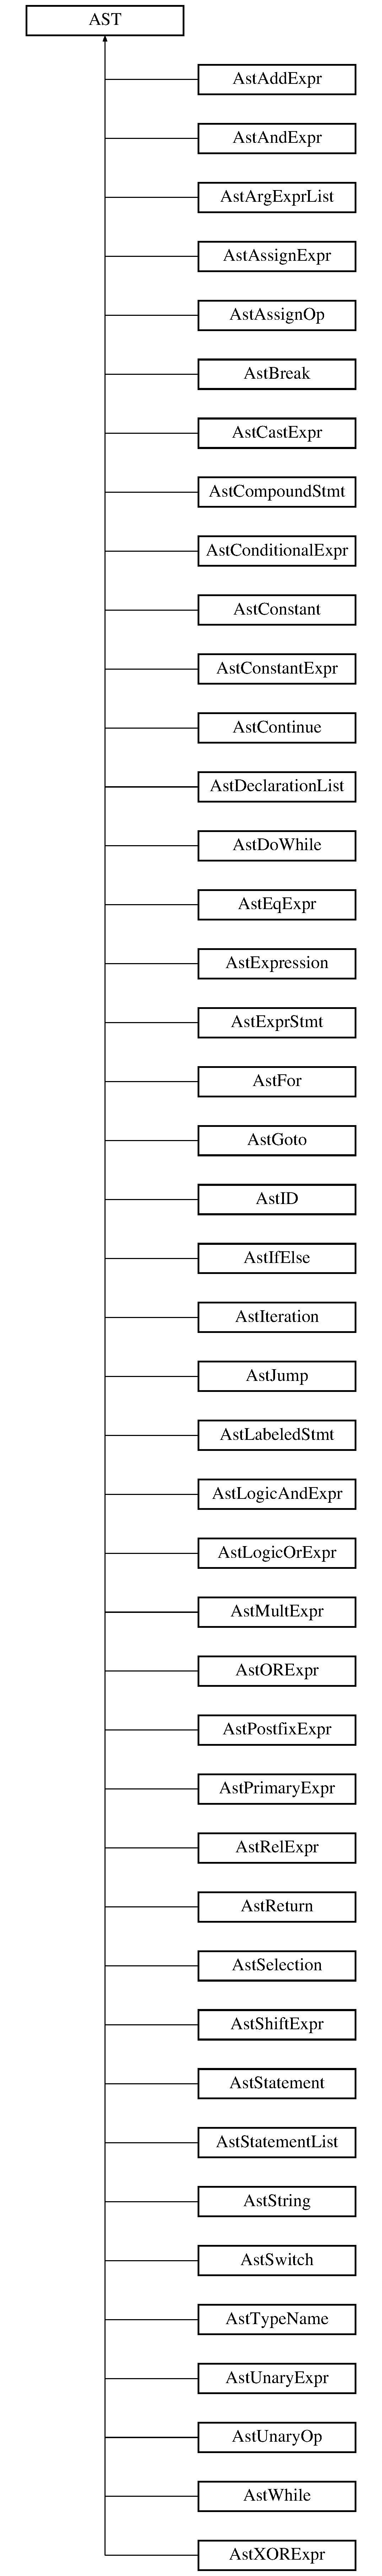
\includegraphics[height=12.000000cm]{classAST}
\end{center}
\end{figure}
\subsection*{Public Member Functions}
\begin{DoxyCompactItemize}
\item 
\hyperlink{classAST_afd378ca7cb3049d6293e8597d31d758d}{A\-S\-T} ()
\begin{DoxyCompactList}\small\item\em \hyperlink{classAST}{A\-S\-T} default constructor. \end{DoxyCompactList}\item 
void \hyperlink{classAST_a71d680856e95ff89f55d5311a552eba6}{set\-Label} (string l)
\begin{DoxyCompactList}\small\item\em Sets the label for the node. \end{DoxyCompactList}\item 
int \hyperlink{classAST_ab7a5b1d9f1c2de0d98deb356f724a42c}{get\-U\-I\-D} ()
\begin{DoxyCompactList}\small\item\em Gets the node's unique I\-D. \end{DoxyCompactList}\item 
string \hyperlink{classAST_aee029be902fffc927d16ccb03eb922ad}{get\-Label} ()
\begin{DoxyCompactList}\small\item\em Gets the node's label. \end{DoxyCompactList}\item 
virtual void \hyperlink{classAST_a5828cc86f2c4f1a0aeab6d7069e8fd82}{Visit} ()
\begin{DoxyCompactList}\small\item\em This function is responsible for tree traversals. \end{DoxyCompactList}\item 
\hyperlink{classAST_afd378ca7cb3049d6293e8597d31d758d}{A\-S\-T} ()
\begin{DoxyCompactList}\small\item\em \hyperlink{classAST}{A\-S\-T} default constructor. \end{DoxyCompactList}\item 
void \hyperlink{classAST_a71d680856e95ff89f55d5311a552eba6}{set\-Label} (string l)
\begin{DoxyCompactList}\small\item\em Sets the label for the node. \end{DoxyCompactList}\item 
int \hyperlink{classAST_ab7a5b1d9f1c2de0d98deb356f724a42c}{get\-U\-I\-D} ()
\begin{DoxyCompactList}\small\item\em Gets the node's unique I\-D. \end{DoxyCompactList}\item 
string \hyperlink{classAST_aee029be902fffc927d16ccb03eb922ad}{get\-Label} ()
\begin{DoxyCompactList}\small\item\em Gets the node's label. \end{DoxyCompactList}\item 
virtual void \hyperlink{classAST_a5828cc86f2c4f1a0aeab6d7069e8fd82}{Visit} ()
\begin{DoxyCompactList}\small\item\em This function is responsible for tree traversals. \end{DoxyCompactList}\item 
\hyperlink{classAST_afd378ca7cb3049d6293e8597d31d758d}{A\-S\-T} ()
\begin{DoxyCompactList}\small\item\em \hyperlink{classAST}{A\-S\-T} default constructor. \end{DoxyCompactList}\item 
void \hyperlink{classAST_a71d680856e95ff89f55d5311a552eba6}{set\-Label} (string l)
\begin{DoxyCompactList}\small\item\em Sets the label for the node. \end{DoxyCompactList}\item 
int \hyperlink{classAST_ab7a5b1d9f1c2de0d98deb356f724a42c}{get\-U\-I\-D} ()
\begin{DoxyCompactList}\small\item\em Gets the node's unique I\-D. \end{DoxyCompactList}\item 
string \hyperlink{classAST_aee029be902fffc927d16ccb03eb922ad}{get\-Label} ()
\begin{DoxyCompactList}\small\item\em Gets the node's label. \end{DoxyCompactList}\item 
virtual void \hyperlink{classAST_a5828cc86f2c4f1a0aeab6d7069e8fd82}{Visit} ()
\begin{DoxyCompactList}\small\item\em This function is responsible for tree traversals. \end{DoxyCompactList}\item 
\hyperlink{classAST_afd378ca7cb3049d6293e8597d31d758d}{A\-S\-T} ()
\begin{DoxyCompactList}\small\item\em \hyperlink{classAST}{A\-S\-T} default constructor. \end{DoxyCompactList}\item 
void \hyperlink{classAST_a71d680856e95ff89f55d5311a552eba6}{set\-Label} (string l)
\begin{DoxyCompactList}\small\item\em Sets the label for the node. \end{DoxyCompactList}\item 
int \hyperlink{classAST_ab7a5b1d9f1c2de0d98deb356f724a42c}{get\-U\-I\-D} ()
\begin{DoxyCompactList}\small\item\em Gets the node's unique I\-D. \end{DoxyCompactList}\item 
string \hyperlink{classAST_aee029be902fffc927d16ccb03eb922ad}{get\-Label} ()
\begin{DoxyCompactList}\small\item\em Gets the node's label. \end{DoxyCompactList}\item 
virtual void \hyperlink{classAST_a5828cc86f2c4f1a0aeab6d7069e8fd82}{Visit} ()
\begin{DoxyCompactList}\small\item\em This function is responsible for tree traversals. \end{DoxyCompactList}\end{DoxyCompactItemize}
\subsection*{Public Attributes}
\begin{DoxyCompactItemize}
\item 
\hypertarget{classAST_aaf215802de409f8096c063d01ffa6783}{bool \hyperlink{classAST_aaf215802de409f8096c063d01ffa6783}{needs\-Cast}}\label{classAST_aaf215802de409f8096c063d01ffa6783}

\begin{DoxyCompactList}\small\item\em This indicates if cast 3\-A\-C needs to be output, and is only relevant for expressions. \end{DoxyCompactList}\item 
\hypertarget{classAST_afa9e77ef650ec6664458fa6cb55be985}{bool \hyperlink{classAST_afa9e77ef650ec6664458fa6cb55be985}{is\-Conv}}\label{classAST_afa9e77ef650ec6664458fa6cb55be985}

\begin{DoxyCompactList}\small\item\em Indicates is a conversion is possible. \end{DoxyCompactList}\item 
\hypertarget{classAST_a61ef3317e023d45237e06615b387cd6b}{C\-O\-N\-V\-E\-R\-S\-I\-O\-N\-T\-Y\-P\-E \hyperlink{classAST_a61ef3317e023d45237e06615b387cd6b}{conv\-Type}}\label{classAST_a61ef3317e023d45237e06615b387cd6b}

\begin{DoxyCompactList}\small\item\em If needs\-Cast is true, then this indicates what the cast should be. \end{DoxyCompactList}\item 
\hypertarget{classAST_aea9b07b39d24183f38c0029cec0a878e}{int \hyperlink{classAST_aea9b07b39d24183f38c0029cec0a878e}{operand\-To\-Cast}}\label{classAST_aea9b07b39d24183f38c0029cec0a878e}

\begin{DoxyCompactList}\small\item\em This indicates if the first or second operand should be the one that is cast. \end{DoxyCompactList}\end{DoxyCompactItemize}
\subsection*{Static Public Attributes}
\begin{DoxyCompactItemize}
\item 
\hypertarget{classAST_a5fdfd5f7b104dd92889163bdadbc68d6}{static \hyperlink{classVisualizer}{Visualizer} \hyperlink{classAST_a5fdfd5f7b104dd92889163bdadbc68d6}{vis}}\label{classAST_a5fdfd5f7b104dd92889163bdadbc68d6}

\begin{DoxyCompactList}\small\item\em Static visualizer instance for generating the visualization of the \hyperlink{classAST}{A\-S\-T}. \end{DoxyCompactList}\item 
\hypertarget{classAST_a8a3ace322f50e030331065d644ee55ee}{static \hyperlink{classTAC__Generator}{T\-A\-C\-\_\-\-Generator} \hyperlink{classAST_a8a3ace322f50e030331065d644ee55ee}{tac\-Gen}}\label{classAST_a8a3ace322f50e030331065d644ee55ee}

\begin{DoxyCompactList}\small\item\em Three address code generator. \end{DoxyCompactList}\item 
\hypertarget{classAST_a1f69448c6dc368d005631a128460083d}{static string {\bfseries current\-Temp} =\char`\"{}\char`\"{}}\label{classAST_a1f69448c6dc368d005631a128460083d}

\item 
\hypertarget{classAST_a551aec090c932ab69365238b40a8a4eb}{static string \hyperlink{classAST_a551aec090c932ab69365238b40a8a4eb}{return\-Label} =\char`\"{}\char`\"{}}\label{classAST_a551aec090c932ab69365238b40a8a4eb}

\begin{DoxyCompactList}\small\item\em This is for storing the string id of any temporary result register that may be created during 3\-A\-C generation. \end{DoxyCompactList}\item 
\hypertarget{classAST_a73c0a266df52be71e6b527b6aa635173}{static list$<$ string $>$ {\bfseries temp\-Stack}}\label{classAST_a73c0a266df52be71e6b527b6aa635173}

\item 
\hypertarget{classAST_abf9e84b541ff04b7bb64e6e4371512d4}{static string {\bfseries last\-I\-D} =\char`\"{}\char`\"{}}\label{classAST_abf9e84b541ff04b7bb64e6e4371512d4}

\item 
\hypertarget{classAST_a163003bfe9c30510ec8039870346049f}{static \hyperlink{classSymTab}{Sym\-Tab} $\ast$ {\bfseries symbol\-Table} =N\-U\-L\-L}\label{classAST_a163003bfe9c30510ec8039870346049f}

\item 
\hypertarget{classAST_a5c3cc894d9c0453523dec9ed76f18a04}{static string {\bfseries current\-Function} =\char`\"{}\char`\"{}}\label{classAST_a5c3cc894d9c0453523dec9ed76f18a04}

\end{DoxyCompactItemize}
\subsection*{Protected Attributes}
\begin{DoxyCompactItemize}
\item 
\hypertarget{classAST_a847b778f1c3dd5a19de32de432ee6e15}{int \hyperlink{classAST_a847b778f1c3dd5a19de32de432ee6e15}{uid}}\label{classAST_a847b778f1c3dd5a19de32de432ee6e15}

\begin{DoxyCompactList}\small\item\em The unique id. \end{DoxyCompactList}\item 
\hypertarget{classAST_ab2e239ccc0688d2341724432ff5a1a31}{string \hyperlink{classAST_ab2e239ccc0688d2341724432ff5a1a31}{label}}\label{classAST_ab2e239ccc0688d2341724432ff5a1a31}

\begin{DoxyCompactList}\small\item\em The label to be printed in the visualization. \end{DoxyCompactList}\end{DoxyCompactItemize}


\subsection{Detailed Description}
Abstract syntax tree node type. 

Definition at line 19 of file Ast.\-h.



\subsection{Constructor \& Destructor Documentation}
\hypertarget{classAST_afd378ca7cb3049d6293e8597d31d758d}{\index{A\-S\-T@{A\-S\-T}!A\-S\-T@{A\-S\-T}}
\index{A\-S\-T@{A\-S\-T}!AST@{A\-S\-T}}
\subsubsection[{A\-S\-T}]{\setlength{\rightskip}{0pt plus 5cm}A\-S\-T\-::\-A\-S\-T (
\begin{DoxyParamCaption}
{}
\end{DoxyParamCaption}
)\hspace{0.3cm}{\ttfamily [inline]}}}\label{classAST_afd378ca7cb3049d6293e8597d31d758d}


\hyperlink{classAST}{A\-S\-T} default constructor. 

This default constructor ensures that every node has a label and a unique identifier (used for visualizing the tree) 

Definition at line 27 of file Ast.\-h.

\hypertarget{classAST_afd378ca7cb3049d6293e8597d31d758d}{\index{A\-S\-T@{A\-S\-T}!A\-S\-T@{A\-S\-T}}
\index{A\-S\-T@{A\-S\-T}!AST@{A\-S\-T}}
\subsubsection[{A\-S\-T}]{\setlength{\rightskip}{0pt plus 5cm}A\-S\-T\-::\-A\-S\-T (
\begin{DoxyParamCaption}
{}
\end{DoxyParamCaption}
)\hspace{0.3cm}{\ttfamily [inline]}}}\label{classAST_afd378ca7cb3049d6293e8597d31d758d}


\hyperlink{classAST}{A\-S\-T} default constructor. 

This default constructor ensures that every node has a label and a unique identifier (used for visualizing the tree) 

Definition at line 27 of file C\-Parser.\-yy.

\hypertarget{classAST_afd378ca7cb3049d6293e8597d31d758d}{\index{A\-S\-T@{A\-S\-T}!A\-S\-T@{A\-S\-T}}
\index{A\-S\-T@{A\-S\-T}!AST@{A\-S\-T}}
\subsubsection[{A\-S\-T}]{\setlength{\rightskip}{0pt plus 5cm}A\-S\-T\-::\-A\-S\-T (
\begin{DoxyParamCaption}
{}
\end{DoxyParamCaption}
)\hspace{0.3cm}{\ttfamily [inline]}}}\label{classAST_afd378ca7cb3049d6293e8597d31d758d}


\hyperlink{classAST}{A\-S\-T} default constructor. 

This default constructor ensures that every node has a label and a unique identifier (used for visualizing the tree) 

Definition at line 27 of file C\-Parser.\-yy.

\hypertarget{classAST_afd378ca7cb3049d6293e8597d31d758d}{\index{A\-S\-T@{A\-S\-T}!A\-S\-T@{A\-S\-T}}
\index{A\-S\-T@{A\-S\-T}!AST@{A\-S\-T}}
\subsubsection[{A\-S\-T}]{\setlength{\rightskip}{0pt plus 5cm}A\-S\-T\-::\-A\-S\-T (
\begin{DoxyParamCaption}
{}
\end{DoxyParamCaption}
)\hspace{0.3cm}{\ttfamily [inline]}}}\label{classAST_afd378ca7cb3049d6293e8597d31d758d}


\hyperlink{classAST}{A\-S\-T} default constructor. 

This default constructor ensures that every node has a label and a unique identifier (used for visualizing the tree) 

Definition at line 27 of file C\-Scanner.\-ll.



\subsection{Member Function Documentation}
\hypertarget{classAST_aee029be902fffc927d16ccb03eb922ad}{\index{A\-S\-T@{A\-S\-T}!get\-Label@{get\-Label}}
\index{get\-Label@{get\-Label}!AST@{A\-S\-T}}
\subsubsection[{get\-Label}]{\setlength{\rightskip}{0pt plus 5cm}string A\-S\-T\-::get\-Label (
\begin{DoxyParamCaption}
{}
\end{DoxyParamCaption}
)\hspace{0.3cm}{\ttfamily [inline]}}}\label{classAST_aee029be902fffc927d16ccb03eb922ad}


Gets the node's label. 

\begin{DoxyReturn}{Returns}
The label 
\end{DoxyReturn}


Definition at line 60 of file Ast.\-h.

\hypertarget{classAST_aee029be902fffc927d16ccb03eb922ad}{\index{A\-S\-T@{A\-S\-T}!get\-Label@{get\-Label}}
\index{get\-Label@{get\-Label}!AST@{A\-S\-T}}
\subsubsection[{get\-Label}]{\setlength{\rightskip}{0pt plus 5cm}string A\-S\-T\-::get\-Label (
\begin{DoxyParamCaption}
{}
\end{DoxyParamCaption}
)\hspace{0.3cm}{\ttfamily [inline]}}}\label{classAST_aee029be902fffc927d16ccb03eb922ad}


Gets the node's label. 

\begin{DoxyReturn}{Returns}
The label 
\end{DoxyReturn}


Definition at line 60 of file C\-Parser.\-yy.

\hypertarget{classAST_aee029be902fffc927d16ccb03eb922ad}{\index{A\-S\-T@{A\-S\-T}!get\-Label@{get\-Label}}
\index{get\-Label@{get\-Label}!AST@{A\-S\-T}}
\subsubsection[{get\-Label}]{\setlength{\rightskip}{0pt plus 5cm}string A\-S\-T\-::get\-Label (
\begin{DoxyParamCaption}
{}
\end{DoxyParamCaption}
)\hspace{0.3cm}{\ttfamily [inline]}}}\label{classAST_aee029be902fffc927d16ccb03eb922ad}


Gets the node's label. 

\begin{DoxyReturn}{Returns}
The label 
\end{DoxyReturn}


Definition at line 60 of file C\-Parser.\-yy.

\hypertarget{classAST_aee029be902fffc927d16ccb03eb922ad}{\index{A\-S\-T@{A\-S\-T}!get\-Label@{get\-Label}}
\index{get\-Label@{get\-Label}!AST@{A\-S\-T}}
\subsubsection[{get\-Label}]{\setlength{\rightskip}{0pt plus 5cm}string A\-S\-T\-::get\-Label (
\begin{DoxyParamCaption}
{}
\end{DoxyParamCaption}
)\hspace{0.3cm}{\ttfamily [inline]}}}\label{classAST_aee029be902fffc927d16ccb03eb922ad}


Gets the node's label. 

\begin{DoxyReturn}{Returns}
The label 
\end{DoxyReturn}


Definition at line 60 of file C\-Scanner.\-ll.

\hypertarget{classAST_ab7a5b1d9f1c2de0d98deb356f724a42c}{\index{A\-S\-T@{A\-S\-T}!get\-U\-I\-D@{get\-U\-I\-D}}
\index{get\-U\-I\-D@{get\-U\-I\-D}!AST@{A\-S\-T}}
\subsubsection[{get\-U\-I\-D}]{\setlength{\rightskip}{0pt plus 5cm}int A\-S\-T\-::get\-U\-I\-D (
\begin{DoxyParamCaption}
{}
\end{DoxyParamCaption}
)\hspace{0.3cm}{\ttfamily [inline]}}}\label{classAST_ab7a5b1d9f1c2de0d98deb356f724a42c}


Gets the node's unique I\-D. 

\begin{DoxyReturn}{Returns}
The unique id 
\end{DoxyReturn}


Definition at line 53 of file C\-Parser.\-yy.

\hypertarget{classAST_ab7a5b1d9f1c2de0d98deb356f724a42c}{\index{A\-S\-T@{A\-S\-T}!get\-U\-I\-D@{get\-U\-I\-D}}
\index{get\-U\-I\-D@{get\-U\-I\-D}!AST@{A\-S\-T}}
\subsubsection[{get\-U\-I\-D}]{\setlength{\rightskip}{0pt plus 5cm}int A\-S\-T\-::get\-U\-I\-D (
\begin{DoxyParamCaption}
{}
\end{DoxyParamCaption}
)\hspace{0.3cm}{\ttfamily [inline]}}}\label{classAST_ab7a5b1d9f1c2de0d98deb356f724a42c}


Gets the node's unique I\-D. 

\begin{DoxyReturn}{Returns}
The unique id 
\end{DoxyReturn}


Definition at line 53 of file C\-Scanner.\-ll.

\hypertarget{classAST_ab7a5b1d9f1c2de0d98deb356f724a42c}{\index{A\-S\-T@{A\-S\-T}!get\-U\-I\-D@{get\-U\-I\-D}}
\index{get\-U\-I\-D@{get\-U\-I\-D}!AST@{A\-S\-T}}
\subsubsection[{get\-U\-I\-D}]{\setlength{\rightskip}{0pt plus 5cm}int A\-S\-T\-::get\-U\-I\-D (
\begin{DoxyParamCaption}
{}
\end{DoxyParamCaption}
)\hspace{0.3cm}{\ttfamily [inline]}}}\label{classAST_ab7a5b1d9f1c2de0d98deb356f724a42c}


Gets the node's unique I\-D. 

\begin{DoxyReturn}{Returns}
The unique id 
\end{DoxyReturn}


Definition at line 53 of file C\-Parser.\-yy.

\hypertarget{classAST_ab7a5b1d9f1c2de0d98deb356f724a42c}{\index{A\-S\-T@{A\-S\-T}!get\-U\-I\-D@{get\-U\-I\-D}}
\index{get\-U\-I\-D@{get\-U\-I\-D}!AST@{A\-S\-T}}
\subsubsection[{get\-U\-I\-D}]{\setlength{\rightskip}{0pt plus 5cm}int A\-S\-T\-::get\-U\-I\-D (
\begin{DoxyParamCaption}
{}
\end{DoxyParamCaption}
)\hspace{0.3cm}{\ttfamily [inline]}}}\label{classAST_ab7a5b1d9f1c2de0d98deb356f724a42c}


Gets the node's unique I\-D. 

\begin{DoxyReturn}{Returns}
The unique id 
\end{DoxyReturn}


Definition at line 53 of file Ast.\-h.

\hypertarget{classAST_a71d680856e95ff89f55d5311a552eba6}{\index{A\-S\-T@{A\-S\-T}!set\-Label@{set\-Label}}
\index{set\-Label@{set\-Label}!AST@{A\-S\-T}}
\subsubsection[{set\-Label}]{\setlength{\rightskip}{0pt plus 5cm}void A\-S\-T\-::set\-Label (
\begin{DoxyParamCaption}
\item[{string}]{l}
\end{DoxyParamCaption}
)\hspace{0.3cm}{\ttfamily [inline]}}}\label{classAST_a71d680856e95ff89f55d5311a552eba6}


Sets the label for the node. 


\begin{DoxyParams}{Parameters}
{\em l} & The label string \\
\hline
\end{DoxyParams}


Definition at line 43 of file C\-Scanner.\-ll.

\hypertarget{classAST_a71d680856e95ff89f55d5311a552eba6}{\index{A\-S\-T@{A\-S\-T}!set\-Label@{set\-Label}}
\index{set\-Label@{set\-Label}!AST@{A\-S\-T}}
\subsubsection[{set\-Label}]{\setlength{\rightskip}{0pt plus 5cm}void A\-S\-T\-::set\-Label (
\begin{DoxyParamCaption}
\item[{string}]{l}
\end{DoxyParamCaption}
)\hspace{0.3cm}{\ttfamily [inline]}}}\label{classAST_a71d680856e95ff89f55d5311a552eba6}


Sets the label for the node. 


\begin{DoxyParams}{Parameters}
{\em l} & The label string \\
\hline
\end{DoxyParams}


Definition at line 43 of file C\-Parser.\-yy.

\hypertarget{classAST_a71d680856e95ff89f55d5311a552eba6}{\index{A\-S\-T@{A\-S\-T}!set\-Label@{set\-Label}}
\index{set\-Label@{set\-Label}!AST@{A\-S\-T}}
\subsubsection[{set\-Label}]{\setlength{\rightskip}{0pt plus 5cm}void A\-S\-T\-::set\-Label (
\begin{DoxyParamCaption}
\item[{string}]{l}
\end{DoxyParamCaption}
)\hspace{0.3cm}{\ttfamily [inline]}}}\label{classAST_a71d680856e95ff89f55d5311a552eba6}


Sets the label for the node. 


\begin{DoxyParams}{Parameters}
{\em l} & The label string \\
\hline
\end{DoxyParams}


Definition at line 43 of file C\-Parser.\-yy.

\hypertarget{classAST_a71d680856e95ff89f55d5311a552eba6}{\index{A\-S\-T@{A\-S\-T}!set\-Label@{set\-Label}}
\index{set\-Label@{set\-Label}!AST@{A\-S\-T}}
\subsubsection[{set\-Label}]{\setlength{\rightskip}{0pt plus 5cm}void A\-S\-T\-::set\-Label (
\begin{DoxyParamCaption}
\item[{string}]{l}
\end{DoxyParamCaption}
)\hspace{0.3cm}{\ttfamily [inline]}}}\label{classAST_a71d680856e95ff89f55d5311a552eba6}


Sets the label for the node. 


\begin{DoxyParams}{Parameters}
{\em l} & The label string \\
\hline
\end{DoxyParams}


Definition at line 43 of file Ast.\-h.

\hypertarget{classAST_a5828cc86f2c4f1a0aeab6d7069e8fd82}{\index{A\-S\-T@{A\-S\-T}!Visit@{Visit}}
\index{Visit@{Visit}!AST@{A\-S\-T}}
\subsubsection[{Visit}]{\setlength{\rightskip}{0pt plus 5cm}virtual void A\-S\-T\-::\-Visit (
\begin{DoxyParamCaption}
{}
\end{DoxyParamCaption}
)\hspace{0.3cm}{\ttfamily [inline]}, {\ttfamily [virtual]}}}\label{classAST_a5828cc86f2c4f1a0aeab6d7069e8fd82}


This function is responsible for tree traversals. 

This function will call the Visit functions of each of it's children nodes, call the visualization code for itself, and output any 3\-A\-C that can be generated at the current node. 

Reimplemented in \hyperlink{classAstFuncDef_a0efb4691e607864f5fb3ffa3a0dfde95}{Ast\-Func\-Def}, \hyperlink{classAstFuncDef_a0efb4691e607864f5fb3ffa3a0dfde95}{Ast\-Func\-Def}, \hyperlink{classAstFuncDef_a0efb4691e607864f5fb3ffa3a0dfde95}{Ast\-Func\-Def}, \hyperlink{classAstFuncDef_a0efb4691e607864f5fb3ffa3a0dfde95}{Ast\-Func\-Def}, \hyperlink{classAstDeclarator_acbc430019c92923e7b33b7f1c409b8a1}{Ast\-Declarator}, \hyperlink{classAstDeclarator_acbc430019c92923e7b33b7f1c409b8a1}{Ast\-Declarator}, \hyperlink{classAstDeclarator_acbc430019c92923e7b33b7f1c409b8a1}{Ast\-Declarator}, \hyperlink{classAstDeclarator_acbc430019c92923e7b33b7f1c409b8a1}{Ast\-Declarator}, \hyperlink{classAstStructDecl_a3044c6bab20d1323fb14854ddc87d4d9}{Ast\-Struct\-Decl}, \hyperlink{classAstStructDecl_a3044c6bab20d1323fb14854ddc87d4d9}{Ast\-Struct\-Decl}, \hyperlink{classAstStructDecl_a3044c6bab20d1323fb14854ddc87d4d9}{Ast\-Struct\-Decl}, \hyperlink{classAstStructDecl_a3044c6bab20d1323fb14854ddc87d4d9}{Ast\-Struct\-Decl}, \hyperlink{classAstSpeciQualList_ac528359b54328d12e59a4abd252bdf38}{Ast\-Speci\-Qual\-List}, \hyperlink{classAstSpeciQualList_ac528359b54328d12e59a4abd252bdf38}{Ast\-Speci\-Qual\-List}, \hyperlink{classAstSpeciQualList_ac528359b54328d12e59a4abd252bdf38}{Ast\-Speci\-Qual\-List}, \hyperlink{classAstSpeciQualList_ac528359b54328d12e59a4abd252bdf38}{Ast\-Speci\-Qual\-List}, \hyperlink{classEnumSpecifier_a73cd1494ac9044c18ea208bb6460f975}{Enum\-Specifier}, \hyperlink{classEnumSpecifier_a73cd1494ac9044c18ea208bb6460f975}{Enum\-Specifier}, \hyperlink{classEnumSpecifier_a73cd1494ac9044c18ea208bb6460f975}{Enum\-Specifier}, \hyperlink{classEnumSpecifier_a73cd1494ac9044c18ea208bb6460f975}{Enum\-Specifier}, \hyperlink{classAstEnumList_a6892acde58e6cd2f807b1449d66b02ea}{Ast\-Enum\-List}, \hyperlink{classAstEnumList_a6892acde58e6cd2f807b1449d66b02ea}{Ast\-Enum\-List}, \hyperlink{classAstEnumList_a6892acde58e6cd2f807b1449d66b02ea}{Ast\-Enum\-List}, \hyperlink{classAstEnumList_a6892acde58e6cd2f807b1449d66b02ea}{Ast\-Enum\-List}, \hyperlink{classAstEnumerator_ab18ef24eeba24051ce318de2c5df57e3}{Ast\-Enumerator}, \hyperlink{classAstEnumerator_ab18ef24eeba24051ce318de2c5df57e3}{Ast\-Enumerator}, \hyperlink{classAstEnumerator_ab18ef24eeba24051ce318de2c5df57e3}{Ast\-Enumerator}, \hyperlink{classAstEnumerator_ab18ef24eeba24051ce318de2c5df57e3}{Ast\-Enumerator}, \hyperlink{classAstInitializer_afe31daa0550b90e8600e4428c259889f}{Ast\-Initializer}, \hyperlink{classAstInitializer_afe31daa0550b90e8600e4428c259889f}{Ast\-Initializer}, \hyperlink{classAstInitializer_afe31daa0550b90e8600e4428c259889f}{Ast\-Initializer}, \hyperlink{classAstInitializer_afe31daa0550b90e8600e4428c259889f}{Ast\-Initializer}, \hyperlink{classAstInitDeclarator_aed19bd7daefcda92d7e223b1fe4d13dd}{Ast\-Init\-Declarator}, \hyperlink{classAstInitDeclarator_aed19bd7daefcda92d7e223b1fe4d13dd}{Ast\-Init\-Declarator}, \hyperlink{classAstInitDeclarator_aed19bd7daefcda92d7e223b1fe4d13dd}{Ast\-Init\-Declarator}, \hyperlink{classAstInitDeclarator_aed19bd7daefcda92d7e223b1fe4d13dd}{Ast\-Init\-Declarator}, \hyperlink{classAstInitDeclList_a65814097bf9a6b3adf22b24b44a94d14}{Ast\-Init\-Decl\-List}, \hyperlink{classAstInitDeclList_a65814097bf9a6b3adf22b24b44a94d14}{Ast\-Init\-Decl\-List}, \hyperlink{classAstInitDeclList_a65814097bf9a6b3adf22b24b44a94d14}{Ast\-Init\-Decl\-List}, \hyperlink{classAstInitDeclList_a65814097bf9a6b3adf22b24b44a94d14}{Ast\-Init\-Decl\-List}, \hyperlink{classAstDirectAbsDecl_a13d80c7a5dc0040b79479d1fcf3ed5c7}{Ast\-Direct\-Abs\-Decl}, \hyperlink{classAstDirectAbsDecl_a13d80c7a5dc0040b79479d1fcf3ed5c7}{Ast\-Direct\-Abs\-Decl}, \hyperlink{classAstDirectAbsDecl_a13d80c7a5dc0040b79479d1fcf3ed5c7}{Ast\-Direct\-Abs\-Decl}, \hyperlink{classAstDirectAbsDecl_a13d80c7a5dc0040b79479d1fcf3ed5c7}{Ast\-Direct\-Abs\-Decl}, \hyperlink{classAstTypeParamList_aa089fa084ef99e8ec0c6a10f946b1076}{Ast\-Type\-Param\-List}, \hyperlink{classAstTypeParamList_aa089fa084ef99e8ec0c6a10f946b1076}{Ast\-Type\-Param\-List}, \hyperlink{classAstTypeParamList_aa089fa084ef99e8ec0c6a10f946b1076}{Ast\-Type\-Param\-List}, \hyperlink{classAstTypeParamList_aa089fa084ef99e8ec0c6a10f946b1076}{Ast\-Type\-Param\-List}, \hyperlink{classAstAbstractDecl_a9dac083b6562bac4b22c2346c2bd543e}{Ast\-Abstract\-Decl}, \hyperlink{classAstAbstractDecl_a9dac083b6562bac4b22c2346c2bd543e}{Ast\-Abstract\-Decl}, \hyperlink{classAstAbstractDecl_a9dac083b6562bac4b22c2346c2bd543e}{Ast\-Abstract\-Decl}, \hyperlink{classAstAbstractDecl_a9dac083b6562bac4b22c2346c2bd543e}{Ast\-Abstract\-Decl}, \hyperlink{classAstDecl_ac70378d3a9b4658624588cb19c80abe4}{Ast\-Decl}, \hyperlink{classAstDecl_ac70378d3a9b4658624588cb19c80abe4}{Ast\-Decl}, \hyperlink{classAstDecl_ac70378d3a9b4658624588cb19c80abe4}{Ast\-Decl}, \hyperlink{classAstDecl_ac70378d3a9b4658624588cb19c80abe4}{Ast\-Decl}, \hyperlink{classAstDeclList_aa142128a4667cc98afb20ff651929acd}{Ast\-Decl\-List}, \hyperlink{classAstDeclList_aa142128a4667cc98afb20ff651929acd}{Ast\-Decl\-List}, \hyperlink{classAstDeclList_aa142128a4667cc98afb20ff651929acd}{Ast\-Decl\-List}, \hyperlink{classAstDeclList_aa142128a4667cc98afb20ff651929acd}{Ast\-Decl\-List}, \hyperlink{classAstDecSpeci_a6f13f2f88633e296f06549ed9375d097}{Ast\-Dec\-Speci}, \hyperlink{classAstDecSpeci_a6f13f2f88633e296f06549ed9375d097}{Ast\-Dec\-Speci}, \hyperlink{classAstDecSpeci_a6f13f2f88633e296f06549ed9375d097}{Ast\-Dec\-Speci}, \hyperlink{classAstDecSpeci_a6f13f2f88633e296f06549ed9375d097}{Ast\-Dec\-Speci}, \hyperlink{classAstDirectDecl_a5f71e3df8a52f41954fa1ce21de05d26}{Ast\-Direct\-Decl}, \hyperlink{classAstDirectDecl_a5f71e3df8a52f41954fa1ce21de05d26}{Ast\-Direct\-Decl}, \hyperlink{classAstDirectDecl_a5f71e3df8a52f41954fa1ce21de05d26}{Ast\-Direct\-Decl}, \hyperlink{classAstDirectDecl_a5f71e3df8a52f41954fa1ce21de05d26}{Ast\-Direct\-Decl}, \hyperlink{classAstStatementList_a3390e533f15c418a597e1eb3b2a14b99}{Ast\-Statement\-List}, \hyperlink{classAstStatementList_a3390e533f15c418a597e1eb3b2a14b99}{Ast\-Statement\-List}, \hyperlink{classAstStatementList_a3390e533f15c418a597e1eb3b2a14b99}{Ast\-Statement\-List}, \hyperlink{classAstStatementList_a3390e533f15c418a597e1eb3b2a14b99}{Ast\-Statement\-List}, \hyperlink{classAstStructDeclList_a6f6f0e09a6a67e65cecda54d8a220a7d}{Ast\-Struct\-Decl\-List}, \hyperlink{classAstStructDeclList_a6f6f0e09a6a67e65cecda54d8a220a7d}{Ast\-Struct\-Decl\-List}, \hyperlink{classAstStructDeclList_a6f6f0e09a6a67e65cecda54d8a220a7d}{Ast\-Struct\-Decl\-List}, \hyperlink{classAstStructDeclList_a6f6f0e09a6a67e65cecda54d8a220a7d}{Ast\-Struct\-Decl\-List}, \hyperlink{classAstTrans_a23f19cce8076b5a2024253c905d7d5dd}{Ast\-Trans}, \hyperlink{classAstTrans_a23f19cce8076b5a2024253c905d7d5dd}{Ast\-Trans}, \hyperlink{classAstTrans_a23f19cce8076b5a2024253c905d7d5dd}{Ast\-Trans}, \hyperlink{classAstTrans_a23f19cce8076b5a2024253c905d7d5dd}{Ast\-Trans}, \hyperlink{classAstTypeQualList_a4f0314a6b1fa687f92953cdaf43a1ed3}{Ast\-Type\-Qual\-List}, \hyperlink{classAstTypeQualList_a4f0314a6b1fa687f92953cdaf43a1ed3}{Ast\-Type\-Qual\-List}, \hyperlink{classAstTypeQualList_a4f0314a6b1fa687f92953cdaf43a1ed3}{Ast\-Type\-Qual\-List}, \hyperlink{classAstTypeQualList_a4f0314a6b1fa687f92953cdaf43a1ed3}{Ast\-Type\-Qual\-List}, \hyperlink{classAstTypeSpeci_a6e264f3293edf997eb4b2197c8da6247}{Ast\-Type\-Speci}, \hyperlink{classAstTypeSpeci_a6e264f3293edf997eb4b2197c8da6247}{Ast\-Type\-Speci}, \hyperlink{classAstTypeSpeci_a6e264f3293edf997eb4b2197c8da6247}{Ast\-Type\-Speci}, \hyperlink{classAstTypeSpeci_a6e264f3293edf997eb4b2197c8da6247}{Ast\-Type\-Speci}, \hyperlink{classAstDeclarationList_a1c98628f55a26aabfacbbb670d2eac12}{Ast\-Declaration\-List}, \hyperlink{classAstDeclarationList_a1c98628f55a26aabfacbbb670d2eac12}{Ast\-Declaration\-List}, \hyperlink{classAstDeclarationList_a1c98628f55a26aabfacbbb670d2eac12}{Ast\-Declaration\-List}, \hyperlink{classAstDeclarationList_a1c98628f55a26aabfacbbb670d2eac12}{Ast\-Declaration\-List}, \hyperlink{classAstIDList_aad1cb50799e6c89a2109520e4563b001}{Ast\-I\-D\-List}, \hyperlink{classAstIDList_aad1cb50799e6c89a2109520e4563b001}{Ast\-I\-D\-List}, \hyperlink{classAstIDList_aad1cb50799e6c89a2109520e4563b001}{Ast\-I\-D\-List}, \hyperlink{classAstIDList_aad1cb50799e6c89a2109520e4563b001}{Ast\-I\-D\-List}, \hyperlink{classAstInitList_aac1576c6d64463b17f0f97bd1ea18afd}{Ast\-Init\-List}, \hyperlink{classAstInitList_aac1576c6d64463b17f0f97bd1ea18afd}{Ast\-Init\-List}, \hyperlink{classAstInitList_aac1576c6d64463b17f0f97bd1ea18afd}{Ast\-Init\-List}, \hyperlink{classAstInitList_aac1576c6d64463b17f0f97bd1ea18afd}{Ast\-Init\-List}, \hyperlink{classAstParamDec_ae18700779476a4f06d39b9ed6037906e}{Ast\-Param\-Dec}, \hyperlink{classAstParamDec_ae18700779476a4f06d39b9ed6037906e}{Ast\-Param\-Dec}, \hyperlink{classAstParamDec_ae18700779476a4f06d39b9ed6037906e}{Ast\-Param\-Dec}, \hyperlink{classAstParamDec_ae18700779476a4f06d39b9ed6037906e}{Ast\-Param\-Dec}, \hyperlink{classAstParamList_a9daebed030751c1642d4a435146e49cd}{Ast\-Param\-List}, \hyperlink{classAstParamList_a9daebed030751c1642d4a435146e49cd}{Ast\-Param\-List}, \hyperlink{classAstParamList_a9daebed030751c1642d4a435146e49cd}{Ast\-Param\-List}, \hyperlink{classAstParamList_a9daebed030751c1642d4a435146e49cd}{Ast\-Param\-List}, \hyperlink{classAstPointer_ac3d4a59c8ab0b44963e044bce049a895}{Ast\-Pointer}, \hyperlink{classAstPointer_ac3d4a59c8ab0b44963e044bce049a895}{Ast\-Pointer}, \hyperlink{classAstPointer_ac3d4a59c8ab0b44963e044bce049a895}{Ast\-Pointer}, \hyperlink{classAstPointer_ac3d4a59c8ab0b44963e044bce049a895}{Ast\-Pointer}, \hyperlink{classAstStructDeclarator_a69af8dfada448d1d27dd60d6897e26f1}{Ast\-Struct\-Declarator}, \hyperlink{classAstStructDeclarator_a69af8dfada448d1d27dd60d6897e26f1}{Ast\-Struct\-Declarator}, \hyperlink{classAstStructDeclarator_a69af8dfada448d1d27dd60d6897e26f1}{Ast\-Struct\-Declarator}, \hyperlink{classAstStructDeclarator_a69af8dfada448d1d27dd60d6897e26f1}{Ast\-Struct\-Declarator}, \hyperlink{classAstStructDeclatorList_a848627c085ff17a97221ebc8132366c8}{Ast\-Struct\-Declator\-List}, \hyperlink{classAstStructDeclatorList_a848627c085ff17a97221ebc8132366c8}{Ast\-Struct\-Declator\-List}, \hyperlink{classAstStructDeclatorList_a848627c085ff17a97221ebc8132366c8}{Ast\-Struct\-Declator\-List}, \hyperlink{classAstStructDeclatorList_a848627c085ff17a97221ebc8132366c8}{Ast\-Struct\-Declator\-List}, \hyperlink{classAstStructUniSpeci_aa341c37ae9cd946190d5476f15dfa42a}{Ast\-Struct\-Uni\-Speci}, \hyperlink{classAstStructUniSpeci_aa341c37ae9cd946190d5476f15dfa42a}{Ast\-Struct\-Uni\-Speci}, \hyperlink{classAstStructUniSpeci_aa341c37ae9cd946190d5476f15dfa42a}{Ast\-Struct\-Uni\-Speci}, \hyperlink{classAstStructUniSpeci_aa341c37ae9cd946190d5476f15dfa42a}{Ast\-Struct\-Uni\-Speci}, \hyperlink{classAstStatement_a1f1570931e373fe2f1e18ce417236ee4}{Ast\-Statement}, \hyperlink{classAstStatement_a1f1570931e373fe2f1e18ce417236ee4}{Ast\-Statement}, \hyperlink{classAstStatement_a1f1570931e373fe2f1e18ce417236ee4}{Ast\-Statement}, \hyperlink{classAstStatement_a1f1570931e373fe2f1e18ce417236ee4}{Ast\-Statement}, \hyperlink{classAstLabeledStmt_a2477cd4279ec466452407604e0897261}{Ast\-Labeled\-Stmt}, \hyperlink{classAstLabeledStmt_a2477cd4279ec466452407604e0897261}{Ast\-Labeled\-Stmt}, \hyperlink{classAstLabeledStmt_a2477cd4279ec466452407604e0897261}{Ast\-Labeled\-Stmt}, \hyperlink{classAstLabeledStmt_a2477cd4279ec466452407604e0897261}{Ast\-Labeled\-Stmt}, \hyperlink{classAstExprStmt_aa6763a98f7659d35edf7cf60557609b2}{Ast\-Expr\-Stmt}, \hyperlink{classAstExprStmt_aa6763a98f7659d35edf7cf60557609b2}{Ast\-Expr\-Stmt}, \hyperlink{classAstExprStmt_aa6763a98f7659d35edf7cf60557609b2}{Ast\-Expr\-Stmt}, \hyperlink{classAstExprStmt_aa6763a98f7659d35edf7cf60557609b2}{Ast\-Expr\-Stmt}, \hyperlink{classAstCompoundStmt_a6ff97b453379db290afe4c4c17ad5244}{Ast\-Compound\-Stmt}, \hyperlink{classAstCompoundStmt_a6ff97b453379db290afe4c4c17ad5244}{Ast\-Compound\-Stmt}, \hyperlink{classAstCompoundStmt_a6ff97b453379db290afe4c4c17ad5244}{Ast\-Compound\-Stmt}, \hyperlink{classAstCompoundStmt_a6ff97b453379db290afe4c4c17ad5244}{Ast\-Compound\-Stmt}, \hyperlink{classAstSelection_a811114a424918b2141b5eb0e341c3a22}{Ast\-Selection}, \hyperlink{classAstSelection_a811114a424918b2141b5eb0e341c3a22}{Ast\-Selection}, \hyperlink{classAstSelection_a811114a424918b2141b5eb0e341c3a22}{Ast\-Selection}, \hyperlink{classAstSelection_a811114a424918b2141b5eb0e341c3a22}{Ast\-Selection}, \hyperlink{classAstIfElse_a4c038fd5b0cb99ea75f9847d96f65c32}{Ast\-If\-Else}, \hyperlink{classAstIfElse_a4c038fd5b0cb99ea75f9847d96f65c32}{Ast\-If\-Else}, \hyperlink{classAstIfElse_a4c038fd5b0cb99ea75f9847d96f65c32}{Ast\-If\-Else}, \hyperlink{classAstIfElse_a4c038fd5b0cb99ea75f9847d96f65c32}{Ast\-If\-Else}, \hyperlink{classAstSwitch_a12d5e48474fec08fbf41cb69cffd740a}{Ast\-Switch}, \hyperlink{classAstSwitch_a12d5e48474fec08fbf41cb69cffd740a}{Ast\-Switch}, \hyperlink{classAstSwitch_a12d5e48474fec08fbf41cb69cffd740a}{Ast\-Switch}, \hyperlink{classAstSwitch_a12d5e48474fec08fbf41cb69cffd740a}{Ast\-Switch}, \hyperlink{classAstIteration_ae3e90f781890621279ff29b5481e0d4b}{Ast\-Iteration}, \hyperlink{classAstIteration_ae3e90f781890621279ff29b5481e0d4b}{Ast\-Iteration}, \hyperlink{classAstIteration_ae3e90f781890621279ff29b5481e0d4b}{Ast\-Iteration}, \hyperlink{classAstIteration_ae3e90f781890621279ff29b5481e0d4b}{Ast\-Iteration}, \hyperlink{classAstFor_aabb94ea30de2b634b35c02ec3688d0ff}{Ast\-For}, \hyperlink{classAstFor_aabb94ea30de2b634b35c02ec3688d0ff}{Ast\-For}, \hyperlink{classAstFor_aabb94ea30de2b634b35c02ec3688d0ff}{Ast\-For}, \hyperlink{classAstFor_aabb94ea30de2b634b35c02ec3688d0ff}{Ast\-For}, \hyperlink{classAstWhile_a9bf8eb5f0f63a4f0dc7b7201f292d4dd}{Ast\-While}, \hyperlink{classAstWhile_a9bf8eb5f0f63a4f0dc7b7201f292d4dd}{Ast\-While}, \hyperlink{classAstWhile_a9bf8eb5f0f63a4f0dc7b7201f292d4dd}{Ast\-While}, \hyperlink{classAstWhile_a9bf8eb5f0f63a4f0dc7b7201f292d4dd}{Ast\-While}, \hyperlink{classAstDoWhile_ae45111e771d2b16c5aef452cf37a629f}{Ast\-Do\-While}, \hyperlink{classAstDoWhile_ae45111e771d2b16c5aef452cf37a629f}{Ast\-Do\-While}, \hyperlink{classAstDoWhile_ae45111e771d2b16c5aef452cf37a629f}{Ast\-Do\-While}, \hyperlink{classAstDoWhile_ae45111e771d2b16c5aef452cf37a629f}{Ast\-Do\-While}, \hyperlink{classAstJump_aca65cbe034ffdb439f6e3c73e40550ae}{Ast\-Jump}, \hyperlink{classAstJump_aca65cbe034ffdb439f6e3c73e40550ae}{Ast\-Jump}, \hyperlink{classAstJump_aca65cbe034ffdb439f6e3c73e40550ae}{Ast\-Jump}, \hyperlink{classAstJump_aca65cbe034ffdb439f6e3c73e40550ae}{Ast\-Jump}, \hyperlink{classAstGoto_aa74c48ee01065e4cc79f686bdcfff22a}{Ast\-Goto}, \hyperlink{classAstGoto_aa74c48ee01065e4cc79f686bdcfff22a}{Ast\-Goto}, \hyperlink{classAstGoto_aa74c48ee01065e4cc79f686bdcfff22a}{Ast\-Goto}, \hyperlink{classAstGoto_aa74c48ee01065e4cc79f686bdcfff22a}{Ast\-Goto}, \hyperlink{classAstBreak_added06a2e2ceaec2839df436a6fbf911}{Ast\-Break}, \hyperlink{classAstBreak_added06a2e2ceaec2839df436a6fbf911}{Ast\-Break}, \hyperlink{classAstBreak_added06a2e2ceaec2839df436a6fbf911}{Ast\-Break}, \hyperlink{classAstBreak_added06a2e2ceaec2839df436a6fbf911}{Ast\-Break}, \hyperlink{classAstContinue_a5e3d13c7d6c9077f7a3d50683746c518}{Ast\-Continue}, \hyperlink{classAstContinue_a5e3d13c7d6c9077f7a3d50683746c518}{Ast\-Continue}, \hyperlink{classAstContinue_a5e3d13c7d6c9077f7a3d50683746c518}{Ast\-Continue}, \hyperlink{classAstContinue_a5e3d13c7d6c9077f7a3d50683746c518}{Ast\-Continue}, \hyperlink{classAstReturn_a220df2fba1ee6802b89f55d16821b6ea}{Ast\-Return}, \hyperlink{classAstReturn_a220df2fba1ee6802b89f55d16821b6ea}{Ast\-Return}, \hyperlink{classAstReturn_a220df2fba1ee6802b89f55d16821b6ea}{Ast\-Return}, \hyperlink{classAstReturn_a220df2fba1ee6802b89f55d16821b6ea}{Ast\-Return}, \hyperlink{classAstExpression_acee231d1cd8e4c92393f023bc2f1ecf2}{Ast\-Expression}, \hyperlink{classAstExpression_acee231d1cd8e4c92393f023bc2f1ecf2}{Ast\-Expression}, \hyperlink{classAstExpression_acee231d1cd8e4c92393f023bc2f1ecf2}{Ast\-Expression}, \hyperlink{classAstExpression_acee231d1cd8e4c92393f023bc2f1ecf2}{Ast\-Expression}, \hyperlink{classAstAssignExpr_a7e86da39b9d65e34a16314c0927b78d9}{Ast\-Assign\-Expr}, \hyperlink{classAstAssignExpr_a7e86da39b9d65e34a16314c0927b78d9}{Ast\-Assign\-Expr}, \hyperlink{classAstAssignExpr_a7e86da39b9d65e34a16314c0927b78d9}{Ast\-Assign\-Expr}, \hyperlink{classAstAssignExpr_a7e86da39b9d65e34a16314c0927b78d9}{Ast\-Assign\-Expr}, \hyperlink{classAstAssignOp_a97614556953225b2fedc821732d9fa27}{Ast\-Assign\-Op}, \hyperlink{classAstAssignOp_a97614556953225b2fedc821732d9fa27}{Ast\-Assign\-Op}, \hyperlink{classAstAssignOp_a97614556953225b2fedc821732d9fa27}{Ast\-Assign\-Op}, \hyperlink{classAstAssignOp_a97614556953225b2fedc821732d9fa27}{Ast\-Assign\-Op}, \hyperlink{classAstConstantExpr_a355fbc35bcfa038875468e127527a597}{Ast\-Constant\-Expr}, \hyperlink{classAstConstantExpr_a355fbc35bcfa038875468e127527a597}{Ast\-Constant\-Expr}, \hyperlink{classAstConstantExpr_a355fbc35bcfa038875468e127527a597}{Ast\-Constant\-Expr}, \hyperlink{classAstConstantExpr_a355fbc35bcfa038875468e127527a597}{Ast\-Constant\-Expr}, \hyperlink{classAstConditionalExpr_af62c2b118fd6064ec838435ffa72f48c}{Ast\-Conditional\-Expr}, \hyperlink{classAstConditionalExpr_af62c2b118fd6064ec838435ffa72f48c}{Ast\-Conditional\-Expr}, \hyperlink{classAstConditionalExpr_af62c2b118fd6064ec838435ffa72f48c}{Ast\-Conditional\-Expr}, \hyperlink{classAstConditionalExpr_af62c2b118fd6064ec838435ffa72f48c}{Ast\-Conditional\-Expr}, \hyperlink{classAstLogicOrExpr_acdcdda8eae9c03d8175bbb3527c783eb}{Ast\-Logic\-Or\-Expr}, \hyperlink{classAstLogicOrExpr_acdcdda8eae9c03d8175bbb3527c783eb}{Ast\-Logic\-Or\-Expr}, \hyperlink{classAstLogicOrExpr_acdcdda8eae9c03d8175bbb3527c783eb}{Ast\-Logic\-Or\-Expr}, \hyperlink{classAstLogicOrExpr_acdcdda8eae9c03d8175bbb3527c783eb}{Ast\-Logic\-Or\-Expr}, \hyperlink{classAstLogicAndExpr_a4fc66df5e58e7bea73a712986e94ddcf}{Ast\-Logic\-And\-Expr}, \hyperlink{classAstLogicAndExpr_a4fc66df5e58e7bea73a712986e94ddcf}{Ast\-Logic\-And\-Expr}, \hyperlink{classAstLogicAndExpr_a4fc66df5e58e7bea73a712986e94ddcf}{Ast\-Logic\-And\-Expr}, \hyperlink{classAstLogicAndExpr_a4fc66df5e58e7bea73a712986e94ddcf}{Ast\-Logic\-And\-Expr}, \hyperlink{classAstORExpr_ac442067b01450413dca857727b3af8b3}{Ast\-O\-R\-Expr}, \hyperlink{classAstORExpr_ac442067b01450413dca857727b3af8b3}{Ast\-O\-R\-Expr}, \hyperlink{classAstORExpr_ac442067b01450413dca857727b3af8b3}{Ast\-O\-R\-Expr}, \hyperlink{classAstORExpr_ac442067b01450413dca857727b3af8b3}{Ast\-O\-R\-Expr}, \hyperlink{classAstXORExpr_a6742a6024309a1359fe029204ca50c4f}{Ast\-X\-O\-R\-Expr}, \hyperlink{classAstXORExpr_a6742a6024309a1359fe029204ca50c4f}{Ast\-X\-O\-R\-Expr}, \hyperlink{classAstXORExpr_a6742a6024309a1359fe029204ca50c4f}{Ast\-X\-O\-R\-Expr}, \hyperlink{classAstXORExpr_a6742a6024309a1359fe029204ca50c4f}{Ast\-X\-O\-R\-Expr}, \hyperlink{classAstAndExpr_a0d5cb855afb4a400c2c1a8cda617cf9b}{Ast\-And\-Expr}, \hyperlink{classAstAndExpr_a0d5cb855afb4a400c2c1a8cda617cf9b}{Ast\-And\-Expr}, \hyperlink{classAstAndExpr_a0d5cb855afb4a400c2c1a8cda617cf9b}{Ast\-And\-Expr}, \hyperlink{classAstAndExpr_a0d5cb855afb4a400c2c1a8cda617cf9b}{Ast\-And\-Expr}, \hyperlink{classAstEqExpr_a6e0e9e88f6801eb135efef5bb5fe2851}{Ast\-Eq\-Expr}, \hyperlink{classAstEqExpr_a6e0e9e88f6801eb135efef5bb5fe2851}{Ast\-Eq\-Expr}, \hyperlink{classAstEqExpr_a6e0e9e88f6801eb135efef5bb5fe2851}{Ast\-Eq\-Expr}, \hyperlink{classAstEqExpr_a6e0e9e88f6801eb135efef5bb5fe2851}{Ast\-Eq\-Expr}, \hyperlink{classAstRelExpr_ae1a3ad7c0ce7a205222ec0b1de5ee884}{Ast\-Rel\-Expr}, \hyperlink{classAstRelExpr_ae1a3ad7c0ce7a205222ec0b1de5ee884}{Ast\-Rel\-Expr}, \hyperlink{classAstRelExpr_ae1a3ad7c0ce7a205222ec0b1de5ee884}{Ast\-Rel\-Expr}, \hyperlink{classAstRelExpr_ae1a3ad7c0ce7a205222ec0b1de5ee884}{Ast\-Rel\-Expr}, \hyperlink{classAstShiftExpr_ae20f0c9604ec1ca74911337e3ed375e5}{Ast\-Shift\-Expr}, \hyperlink{classAstShiftExpr_ae20f0c9604ec1ca74911337e3ed375e5}{Ast\-Shift\-Expr}, \hyperlink{classAstShiftExpr_ae20f0c9604ec1ca74911337e3ed375e5}{Ast\-Shift\-Expr}, \hyperlink{classAstShiftExpr_ae20f0c9604ec1ca74911337e3ed375e5}{Ast\-Shift\-Expr}, \hyperlink{classAstAddExpr_a9b80132c7e2f4378ef699cd1de46fa01}{Ast\-Add\-Expr}, \hyperlink{classAstAddExpr_a9b80132c7e2f4378ef699cd1de46fa01}{Ast\-Add\-Expr}, \hyperlink{classAstAddExpr_a9b80132c7e2f4378ef699cd1de46fa01}{Ast\-Add\-Expr}, \hyperlink{classAstAddExpr_a9b80132c7e2f4378ef699cd1de46fa01}{Ast\-Add\-Expr}, \hyperlink{classAstMultExpr_aea6419ae54b97e882c9a9ab79ca73529}{Ast\-Mult\-Expr}, \hyperlink{classAstMultExpr_aea6419ae54b97e882c9a9ab79ca73529}{Ast\-Mult\-Expr}, \hyperlink{classAstMultExpr_aea6419ae54b97e882c9a9ab79ca73529}{Ast\-Mult\-Expr}, \hyperlink{classAstMultExpr_aea6419ae54b97e882c9a9ab79ca73529}{Ast\-Mult\-Expr}, \hyperlink{classAstCastExpr_a5c0f13da0e4bd315eb0e56c9cc9635e9}{Ast\-Cast\-Expr}, \hyperlink{classAstCastExpr_a5c0f13da0e4bd315eb0e56c9cc9635e9}{Ast\-Cast\-Expr}, \hyperlink{classAstCastExpr_a5c0f13da0e4bd315eb0e56c9cc9635e9}{Ast\-Cast\-Expr}, \hyperlink{classAstCastExpr_a5c0f13da0e4bd315eb0e56c9cc9635e9}{Ast\-Cast\-Expr}, \hyperlink{classAstUnaryExpr_ae35427088d6f5c889e8e80573a3750fc}{Ast\-Unary\-Expr}, \hyperlink{classAstUnaryExpr_ae35427088d6f5c889e8e80573a3750fc}{Ast\-Unary\-Expr}, \hyperlink{classAstUnaryExpr_ae35427088d6f5c889e8e80573a3750fc}{Ast\-Unary\-Expr}, \hyperlink{classAstUnaryExpr_ae35427088d6f5c889e8e80573a3750fc}{Ast\-Unary\-Expr}, \hyperlink{classAstPostfixExpr_ae3e7fdbd4c2bf888ee62760e6f422cad}{Ast\-Postfix\-Expr}, \hyperlink{classAstPostfixExpr_ae3e7fdbd4c2bf888ee62760e6f422cad}{Ast\-Postfix\-Expr}, \hyperlink{classAstPostfixExpr_ae3e7fdbd4c2bf888ee62760e6f422cad}{Ast\-Postfix\-Expr}, \hyperlink{classAstPostfixExpr_ae3e7fdbd4c2bf888ee62760e6f422cad}{Ast\-Postfix\-Expr}, \hyperlink{classAstArgExprList_aeac192a90197b0de59114cea84a1e577}{Ast\-Arg\-Expr\-List}, \hyperlink{classAstArgExprList_aeac192a90197b0de59114cea84a1e577}{Ast\-Arg\-Expr\-List}, \hyperlink{classAstArgExprList_aeac192a90197b0de59114cea84a1e577}{Ast\-Arg\-Expr\-List}, \hyperlink{classAstArgExprList_aeac192a90197b0de59114cea84a1e577}{Ast\-Arg\-Expr\-List}, \hyperlink{classAstPrimaryExpr_adfc316933183cada2963b7b855ddb824}{Ast\-Primary\-Expr}, \hyperlink{classAstPrimaryExpr_adfc316933183cada2963b7b855ddb824}{Ast\-Primary\-Expr}, \hyperlink{classAstPrimaryExpr_adfc316933183cada2963b7b855ddb824}{Ast\-Primary\-Expr}, \hyperlink{classAstPrimaryExpr_adfc316933183cada2963b7b855ddb824}{Ast\-Primary\-Expr}, \hyperlink{classAstID_af84d100fc8e77d534362310f36855ad0}{Ast\-I\-D}, \hyperlink{classAstID_af84d100fc8e77d534362310f36855ad0}{Ast\-I\-D}, \hyperlink{classAstID_af84d100fc8e77d534362310f36855ad0}{Ast\-I\-D}, \hyperlink{classAstID_af84d100fc8e77d534362310f36855ad0}{Ast\-I\-D}, \hyperlink{classAstUnaryOp_a23e13d42f33d5882d58ca48e8053f1a0}{Ast\-Unary\-Op}, \hyperlink{classAstUnaryOp_a23e13d42f33d5882d58ca48e8053f1a0}{Ast\-Unary\-Op}, \hyperlink{classAstUnaryOp_a23e13d42f33d5882d58ca48e8053f1a0}{Ast\-Unary\-Op}, \hyperlink{classAstUnaryOp_a23e13d42f33d5882d58ca48e8053f1a0}{Ast\-Unary\-Op}, \hyperlink{classAstConstant_ac13b7246f9d646a5ff00efee4c39bc6b}{Ast\-Constant}, \hyperlink{classAstConstant_ac13b7246f9d646a5ff00efee4c39bc6b}{Ast\-Constant}, \hyperlink{classAstConstant_ac13b7246f9d646a5ff00efee4c39bc6b}{Ast\-Constant}, \hyperlink{classAstConstant_ac13b7246f9d646a5ff00efee4c39bc6b}{Ast\-Constant}, \hyperlink{classAstString_a0a7a6576cf72bfbcd2f78c7ffb9350bb}{Ast\-String}, \hyperlink{classAstString_a0a7a6576cf72bfbcd2f78c7ffb9350bb}{Ast\-String}, \hyperlink{classAstString_a0a7a6576cf72bfbcd2f78c7ffb9350bb}{Ast\-String}, \hyperlink{classAstString_a0a7a6576cf72bfbcd2f78c7ffb9350bb}{Ast\-String}, \hyperlink{classAstTypeName_adcd2b22b4135cadd7b9117e25a5dff45}{Ast\-Type\-Name}, \hyperlink{classAstTypeName_adcd2b22b4135cadd7b9117e25a5dff45}{Ast\-Type\-Name}, \hyperlink{classAstTypeName_adcd2b22b4135cadd7b9117e25a5dff45}{Ast\-Type\-Name}, and \hyperlink{classAstTypeName_adcd2b22b4135cadd7b9117e25a5dff45}{Ast\-Type\-Name}.



Definition at line 74 of file C\-Parser.\-yy.

\hypertarget{classAST_a5828cc86f2c4f1a0aeab6d7069e8fd82}{\index{A\-S\-T@{A\-S\-T}!Visit@{Visit}}
\index{Visit@{Visit}!AST@{A\-S\-T}}
\subsubsection[{Visit}]{\setlength{\rightskip}{0pt plus 5cm}virtual void A\-S\-T\-::\-Visit (
\begin{DoxyParamCaption}
{}
\end{DoxyParamCaption}
)\hspace{0.3cm}{\ttfamily [inline]}, {\ttfamily [virtual]}}}\label{classAST_a5828cc86f2c4f1a0aeab6d7069e8fd82}


This function is responsible for tree traversals. 

This function will call the Visit functions of each of it's children nodes, call the visualization code for itself, and output any 3\-A\-C that can be generated at the current node. 

Reimplemented in \hyperlink{classAstFuncDef_a0efb4691e607864f5fb3ffa3a0dfde95}{Ast\-Func\-Def}, \hyperlink{classAstFuncDef_a0efb4691e607864f5fb3ffa3a0dfde95}{Ast\-Func\-Def}, \hyperlink{classAstFuncDef_a0efb4691e607864f5fb3ffa3a0dfde95}{Ast\-Func\-Def}, \hyperlink{classAstFuncDef_a0efb4691e607864f5fb3ffa3a0dfde95}{Ast\-Func\-Def}, \hyperlink{classAstDeclarator_acbc430019c92923e7b33b7f1c409b8a1}{Ast\-Declarator}, \hyperlink{classAstDeclarator_acbc430019c92923e7b33b7f1c409b8a1}{Ast\-Declarator}, \hyperlink{classAstDeclarator_acbc430019c92923e7b33b7f1c409b8a1}{Ast\-Declarator}, \hyperlink{classAstDeclarator_acbc430019c92923e7b33b7f1c409b8a1}{Ast\-Declarator}, \hyperlink{classAstStructDecl_a3044c6bab20d1323fb14854ddc87d4d9}{Ast\-Struct\-Decl}, \hyperlink{classAstStructDecl_a3044c6bab20d1323fb14854ddc87d4d9}{Ast\-Struct\-Decl}, \hyperlink{classAstStructDecl_a3044c6bab20d1323fb14854ddc87d4d9}{Ast\-Struct\-Decl}, \hyperlink{classAstStructDecl_a3044c6bab20d1323fb14854ddc87d4d9}{Ast\-Struct\-Decl}, \hyperlink{classAstSpeciQualList_ac528359b54328d12e59a4abd252bdf38}{Ast\-Speci\-Qual\-List}, \hyperlink{classAstSpeciQualList_ac528359b54328d12e59a4abd252bdf38}{Ast\-Speci\-Qual\-List}, \hyperlink{classAstSpeciQualList_ac528359b54328d12e59a4abd252bdf38}{Ast\-Speci\-Qual\-List}, \hyperlink{classAstSpeciQualList_ac528359b54328d12e59a4abd252bdf38}{Ast\-Speci\-Qual\-List}, \hyperlink{classEnumSpecifier_a73cd1494ac9044c18ea208bb6460f975}{Enum\-Specifier}, \hyperlink{classEnumSpecifier_a73cd1494ac9044c18ea208bb6460f975}{Enum\-Specifier}, \hyperlink{classEnumSpecifier_a73cd1494ac9044c18ea208bb6460f975}{Enum\-Specifier}, \hyperlink{classEnumSpecifier_a73cd1494ac9044c18ea208bb6460f975}{Enum\-Specifier}, \hyperlink{classAstEnumList_a6892acde58e6cd2f807b1449d66b02ea}{Ast\-Enum\-List}, \hyperlink{classAstEnumList_a6892acde58e6cd2f807b1449d66b02ea}{Ast\-Enum\-List}, \hyperlink{classAstEnumList_a6892acde58e6cd2f807b1449d66b02ea}{Ast\-Enum\-List}, \hyperlink{classAstEnumList_a6892acde58e6cd2f807b1449d66b02ea}{Ast\-Enum\-List}, \hyperlink{classAstEnumerator_ab18ef24eeba24051ce318de2c5df57e3}{Ast\-Enumerator}, \hyperlink{classAstEnumerator_ab18ef24eeba24051ce318de2c5df57e3}{Ast\-Enumerator}, \hyperlink{classAstEnumerator_ab18ef24eeba24051ce318de2c5df57e3}{Ast\-Enumerator}, \hyperlink{classAstEnumerator_ab18ef24eeba24051ce318de2c5df57e3}{Ast\-Enumerator}, \hyperlink{classAstInitializer_afe31daa0550b90e8600e4428c259889f}{Ast\-Initializer}, \hyperlink{classAstInitializer_afe31daa0550b90e8600e4428c259889f}{Ast\-Initializer}, \hyperlink{classAstInitializer_afe31daa0550b90e8600e4428c259889f}{Ast\-Initializer}, \hyperlink{classAstInitializer_afe31daa0550b90e8600e4428c259889f}{Ast\-Initializer}, \hyperlink{classAstInitDeclarator_aed19bd7daefcda92d7e223b1fe4d13dd}{Ast\-Init\-Declarator}, \hyperlink{classAstInitDeclarator_aed19bd7daefcda92d7e223b1fe4d13dd}{Ast\-Init\-Declarator}, \hyperlink{classAstInitDeclarator_aed19bd7daefcda92d7e223b1fe4d13dd}{Ast\-Init\-Declarator}, \hyperlink{classAstInitDeclarator_aed19bd7daefcda92d7e223b1fe4d13dd}{Ast\-Init\-Declarator}, \hyperlink{classAstInitDeclList_a65814097bf9a6b3adf22b24b44a94d14}{Ast\-Init\-Decl\-List}, \hyperlink{classAstInitDeclList_a65814097bf9a6b3adf22b24b44a94d14}{Ast\-Init\-Decl\-List}, \hyperlink{classAstInitDeclList_a65814097bf9a6b3adf22b24b44a94d14}{Ast\-Init\-Decl\-List}, \hyperlink{classAstInitDeclList_a65814097bf9a6b3adf22b24b44a94d14}{Ast\-Init\-Decl\-List}, \hyperlink{classAstDirectAbsDecl_a13d80c7a5dc0040b79479d1fcf3ed5c7}{Ast\-Direct\-Abs\-Decl}, \hyperlink{classAstDirectAbsDecl_a13d80c7a5dc0040b79479d1fcf3ed5c7}{Ast\-Direct\-Abs\-Decl}, \hyperlink{classAstDirectAbsDecl_a13d80c7a5dc0040b79479d1fcf3ed5c7}{Ast\-Direct\-Abs\-Decl}, \hyperlink{classAstDirectAbsDecl_a13d80c7a5dc0040b79479d1fcf3ed5c7}{Ast\-Direct\-Abs\-Decl}, \hyperlink{classAstTypeParamList_aa089fa084ef99e8ec0c6a10f946b1076}{Ast\-Type\-Param\-List}, \hyperlink{classAstTypeParamList_aa089fa084ef99e8ec0c6a10f946b1076}{Ast\-Type\-Param\-List}, \hyperlink{classAstTypeParamList_aa089fa084ef99e8ec0c6a10f946b1076}{Ast\-Type\-Param\-List}, \hyperlink{classAstTypeParamList_aa089fa084ef99e8ec0c6a10f946b1076}{Ast\-Type\-Param\-List}, \hyperlink{classAstAbstractDecl_a9dac083b6562bac4b22c2346c2bd543e}{Ast\-Abstract\-Decl}, \hyperlink{classAstAbstractDecl_a9dac083b6562bac4b22c2346c2bd543e}{Ast\-Abstract\-Decl}, \hyperlink{classAstAbstractDecl_a9dac083b6562bac4b22c2346c2bd543e}{Ast\-Abstract\-Decl}, \hyperlink{classAstAbstractDecl_a9dac083b6562bac4b22c2346c2bd543e}{Ast\-Abstract\-Decl}, \hyperlink{classAstDecl_ac70378d3a9b4658624588cb19c80abe4}{Ast\-Decl}, \hyperlink{classAstDecl_ac70378d3a9b4658624588cb19c80abe4}{Ast\-Decl}, \hyperlink{classAstDecl_ac70378d3a9b4658624588cb19c80abe4}{Ast\-Decl}, \hyperlink{classAstDecl_ac70378d3a9b4658624588cb19c80abe4}{Ast\-Decl}, \hyperlink{classAstDeclList_aa142128a4667cc98afb20ff651929acd}{Ast\-Decl\-List}, \hyperlink{classAstDeclList_aa142128a4667cc98afb20ff651929acd}{Ast\-Decl\-List}, \hyperlink{classAstDeclList_aa142128a4667cc98afb20ff651929acd}{Ast\-Decl\-List}, \hyperlink{classAstDeclList_aa142128a4667cc98afb20ff651929acd}{Ast\-Decl\-List}, \hyperlink{classAstDecSpeci_a6f13f2f88633e296f06549ed9375d097}{Ast\-Dec\-Speci}, \hyperlink{classAstDecSpeci_a6f13f2f88633e296f06549ed9375d097}{Ast\-Dec\-Speci}, \hyperlink{classAstDecSpeci_a6f13f2f88633e296f06549ed9375d097}{Ast\-Dec\-Speci}, \hyperlink{classAstDecSpeci_a6f13f2f88633e296f06549ed9375d097}{Ast\-Dec\-Speci}, \hyperlink{classAstDirectDecl_a5f71e3df8a52f41954fa1ce21de05d26}{Ast\-Direct\-Decl}, \hyperlink{classAstDirectDecl_a5f71e3df8a52f41954fa1ce21de05d26}{Ast\-Direct\-Decl}, \hyperlink{classAstDirectDecl_a5f71e3df8a52f41954fa1ce21de05d26}{Ast\-Direct\-Decl}, \hyperlink{classAstDirectDecl_a5f71e3df8a52f41954fa1ce21de05d26}{Ast\-Direct\-Decl}, \hyperlink{classAstStatementList_a3390e533f15c418a597e1eb3b2a14b99}{Ast\-Statement\-List}, \hyperlink{classAstStatementList_a3390e533f15c418a597e1eb3b2a14b99}{Ast\-Statement\-List}, \hyperlink{classAstStatementList_a3390e533f15c418a597e1eb3b2a14b99}{Ast\-Statement\-List}, \hyperlink{classAstStatementList_a3390e533f15c418a597e1eb3b2a14b99}{Ast\-Statement\-List}, \hyperlink{classAstStructDeclList_a6f6f0e09a6a67e65cecda54d8a220a7d}{Ast\-Struct\-Decl\-List}, \hyperlink{classAstStructDeclList_a6f6f0e09a6a67e65cecda54d8a220a7d}{Ast\-Struct\-Decl\-List}, \hyperlink{classAstStructDeclList_a6f6f0e09a6a67e65cecda54d8a220a7d}{Ast\-Struct\-Decl\-List}, \hyperlink{classAstStructDeclList_a6f6f0e09a6a67e65cecda54d8a220a7d}{Ast\-Struct\-Decl\-List}, \hyperlink{classAstTrans_a23f19cce8076b5a2024253c905d7d5dd}{Ast\-Trans}, \hyperlink{classAstTrans_a23f19cce8076b5a2024253c905d7d5dd}{Ast\-Trans}, \hyperlink{classAstTrans_a23f19cce8076b5a2024253c905d7d5dd}{Ast\-Trans}, \hyperlink{classAstTrans_a23f19cce8076b5a2024253c905d7d5dd}{Ast\-Trans}, \hyperlink{classAstTypeQualList_a4f0314a6b1fa687f92953cdaf43a1ed3}{Ast\-Type\-Qual\-List}, \hyperlink{classAstTypeQualList_a4f0314a6b1fa687f92953cdaf43a1ed3}{Ast\-Type\-Qual\-List}, \hyperlink{classAstTypeQualList_a4f0314a6b1fa687f92953cdaf43a1ed3}{Ast\-Type\-Qual\-List}, \hyperlink{classAstTypeQualList_a4f0314a6b1fa687f92953cdaf43a1ed3}{Ast\-Type\-Qual\-List}, \hyperlink{classAstTypeSpeci_a6e264f3293edf997eb4b2197c8da6247}{Ast\-Type\-Speci}, \hyperlink{classAstTypeSpeci_a6e264f3293edf997eb4b2197c8da6247}{Ast\-Type\-Speci}, \hyperlink{classAstTypeSpeci_a6e264f3293edf997eb4b2197c8da6247}{Ast\-Type\-Speci}, \hyperlink{classAstTypeSpeci_a6e264f3293edf997eb4b2197c8da6247}{Ast\-Type\-Speci}, \hyperlink{classAstDeclarationList_a1c98628f55a26aabfacbbb670d2eac12}{Ast\-Declaration\-List}, \hyperlink{classAstDeclarationList_a1c98628f55a26aabfacbbb670d2eac12}{Ast\-Declaration\-List}, \hyperlink{classAstDeclarationList_a1c98628f55a26aabfacbbb670d2eac12}{Ast\-Declaration\-List}, \hyperlink{classAstDeclarationList_a1c98628f55a26aabfacbbb670d2eac12}{Ast\-Declaration\-List}, \hyperlink{classAstIDList_aad1cb50799e6c89a2109520e4563b001}{Ast\-I\-D\-List}, \hyperlink{classAstIDList_aad1cb50799e6c89a2109520e4563b001}{Ast\-I\-D\-List}, \hyperlink{classAstIDList_aad1cb50799e6c89a2109520e4563b001}{Ast\-I\-D\-List}, \hyperlink{classAstIDList_aad1cb50799e6c89a2109520e4563b001}{Ast\-I\-D\-List}, \hyperlink{classAstInitList_aac1576c6d64463b17f0f97bd1ea18afd}{Ast\-Init\-List}, \hyperlink{classAstInitList_aac1576c6d64463b17f0f97bd1ea18afd}{Ast\-Init\-List}, \hyperlink{classAstInitList_aac1576c6d64463b17f0f97bd1ea18afd}{Ast\-Init\-List}, \hyperlink{classAstInitList_aac1576c6d64463b17f0f97bd1ea18afd}{Ast\-Init\-List}, \hyperlink{classAstParamDec_ae18700779476a4f06d39b9ed6037906e}{Ast\-Param\-Dec}, \hyperlink{classAstParamDec_ae18700779476a4f06d39b9ed6037906e}{Ast\-Param\-Dec}, \hyperlink{classAstParamDec_ae18700779476a4f06d39b9ed6037906e}{Ast\-Param\-Dec}, \hyperlink{classAstParamDec_ae18700779476a4f06d39b9ed6037906e}{Ast\-Param\-Dec}, \hyperlink{classAstParamList_a9daebed030751c1642d4a435146e49cd}{Ast\-Param\-List}, \hyperlink{classAstParamList_a9daebed030751c1642d4a435146e49cd}{Ast\-Param\-List}, \hyperlink{classAstParamList_a9daebed030751c1642d4a435146e49cd}{Ast\-Param\-List}, \hyperlink{classAstParamList_a9daebed030751c1642d4a435146e49cd}{Ast\-Param\-List}, \hyperlink{classAstPointer_ac3d4a59c8ab0b44963e044bce049a895}{Ast\-Pointer}, \hyperlink{classAstPointer_ac3d4a59c8ab0b44963e044bce049a895}{Ast\-Pointer}, \hyperlink{classAstPointer_ac3d4a59c8ab0b44963e044bce049a895}{Ast\-Pointer}, \hyperlink{classAstPointer_ac3d4a59c8ab0b44963e044bce049a895}{Ast\-Pointer}, \hyperlink{classAstStructDeclarator_a69af8dfada448d1d27dd60d6897e26f1}{Ast\-Struct\-Declarator}, \hyperlink{classAstStructDeclarator_a69af8dfada448d1d27dd60d6897e26f1}{Ast\-Struct\-Declarator}, \hyperlink{classAstStructDeclarator_a69af8dfada448d1d27dd60d6897e26f1}{Ast\-Struct\-Declarator}, \hyperlink{classAstStructDeclarator_a69af8dfada448d1d27dd60d6897e26f1}{Ast\-Struct\-Declarator}, \hyperlink{classAstStructDeclatorList_a848627c085ff17a97221ebc8132366c8}{Ast\-Struct\-Declator\-List}, \hyperlink{classAstStructDeclatorList_a848627c085ff17a97221ebc8132366c8}{Ast\-Struct\-Declator\-List}, \hyperlink{classAstStructDeclatorList_a848627c085ff17a97221ebc8132366c8}{Ast\-Struct\-Declator\-List}, \hyperlink{classAstStructDeclatorList_a848627c085ff17a97221ebc8132366c8}{Ast\-Struct\-Declator\-List}, \hyperlink{classAstStructUniSpeci_aa341c37ae9cd946190d5476f15dfa42a}{Ast\-Struct\-Uni\-Speci}, \hyperlink{classAstStructUniSpeci_aa341c37ae9cd946190d5476f15dfa42a}{Ast\-Struct\-Uni\-Speci}, \hyperlink{classAstStructUniSpeci_aa341c37ae9cd946190d5476f15dfa42a}{Ast\-Struct\-Uni\-Speci}, \hyperlink{classAstStructUniSpeci_aa341c37ae9cd946190d5476f15dfa42a}{Ast\-Struct\-Uni\-Speci}, \hyperlink{classAstStatement_a1f1570931e373fe2f1e18ce417236ee4}{Ast\-Statement}, \hyperlink{classAstStatement_a1f1570931e373fe2f1e18ce417236ee4}{Ast\-Statement}, \hyperlink{classAstStatement_a1f1570931e373fe2f1e18ce417236ee4}{Ast\-Statement}, \hyperlink{classAstStatement_a1f1570931e373fe2f1e18ce417236ee4}{Ast\-Statement}, \hyperlink{classAstLabeledStmt_a2477cd4279ec466452407604e0897261}{Ast\-Labeled\-Stmt}, \hyperlink{classAstLabeledStmt_a2477cd4279ec466452407604e0897261}{Ast\-Labeled\-Stmt}, \hyperlink{classAstLabeledStmt_a2477cd4279ec466452407604e0897261}{Ast\-Labeled\-Stmt}, \hyperlink{classAstLabeledStmt_a2477cd4279ec466452407604e0897261}{Ast\-Labeled\-Stmt}, \hyperlink{classAstExprStmt_aa6763a98f7659d35edf7cf60557609b2}{Ast\-Expr\-Stmt}, \hyperlink{classAstExprStmt_aa6763a98f7659d35edf7cf60557609b2}{Ast\-Expr\-Stmt}, \hyperlink{classAstExprStmt_aa6763a98f7659d35edf7cf60557609b2}{Ast\-Expr\-Stmt}, \hyperlink{classAstExprStmt_aa6763a98f7659d35edf7cf60557609b2}{Ast\-Expr\-Stmt}, \hyperlink{classAstCompoundStmt_a6ff97b453379db290afe4c4c17ad5244}{Ast\-Compound\-Stmt}, \hyperlink{classAstCompoundStmt_a6ff97b453379db290afe4c4c17ad5244}{Ast\-Compound\-Stmt}, \hyperlink{classAstCompoundStmt_a6ff97b453379db290afe4c4c17ad5244}{Ast\-Compound\-Stmt}, \hyperlink{classAstCompoundStmt_a6ff97b453379db290afe4c4c17ad5244}{Ast\-Compound\-Stmt}, \hyperlink{classAstSelection_a811114a424918b2141b5eb0e341c3a22}{Ast\-Selection}, \hyperlink{classAstSelection_a811114a424918b2141b5eb0e341c3a22}{Ast\-Selection}, \hyperlink{classAstSelection_a811114a424918b2141b5eb0e341c3a22}{Ast\-Selection}, \hyperlink{classAstSelection_a811114a424918b2141b5eb0e341c3a22}{Ast\-Selection}, \hyperlink{classAstIfElse_a4c038fd5b0cb99ea75f9847d96f65c32}{Ast\-If\-Else}, \hyperlink{classAstIfElse_a4c038fd5b0cb99ea75f9847d96f65c32}{Ast\-If\-Else}, \hyperlink{classAstIfElse_a4c038fd5b0cb99ea75f9847d96f65c32}{Ast\-If\-Else}, \hyperlink{classAstIfElse_a4c038fd5b0cb99ea75f9847d96f65c32}{Ast\-If\-Else}, \hyperlink{classAstSwitch_a12d5e48474fec08fbf41cb69cffd740a}{Ast\-Switch}, \hyperlink{classAstSwitch_a12d5e48474fec08fbf41cb69cffd740a}{Ast\-Switch}, \hyperlink{classAstSwitch_a12d5e48474fec08fbf41cb69cffd740a}{Ast\-Switch}, \hyperlink{classAstSwitch_a12d5e48474fec08fbf41cb69cffd740a}{Ast\-Switch}, \hyperlink{classAstIteration_ae3e90f781890621279ff29b5481e0d4b}{Ast\-Iteration}, \hyperlink{classAstIteration_ae3e90f781890621279ff29b5481e0d4b}{Ast\-Iteration}, \hyperlink{classAstIteration_ae3e90f781890621279ff29b5481e0d4b}{Ast\-Iteration}, \hyperlink{classAstIteration_ae3e90f781890621279ff29b5481e0d4b}{Ast\-Iteration}, \hyperlink{classAstFor_aabb94ea30de2b634b35c02ec3688d0ff}{Ast\-For}, \hyperlink{classAstFor_aabb94ea30de2b634b35c02ec3688d0ff}{Ast\-For}, \hyperlink{classAstFor_aabb94ea30de2b634b35c02ec3688d0ff}{Ast\-For}, \hyperlink{classAstFor_aabb94ea30de2b634b35c02ec3688d0ff}{Ast\-For}, \hyperlink{classAstWhile_a9bf8eb5f0f63a4f0dc7b7201f292d4dd}{Ast\-While}, \hyperlink{classAstWhile_a9bf8eb5f0f63a4f0dc7b7201f292d4dd}{Ast\-While}, \hyperlink{classAstWhile_a9bf8eb5f0f63a4f0dc7b7201f292d4dd}{Ast\-While}, \hyperlink{classAstWhile_a9bf8eb5f0f63a4f0dc7b7201f292d4dd}{Ast\-While}, \hyperlink{classAstDoWhile_ae45111e771d2b16c5aef452cf37a629f}{Ast\-Do\-While}, \hyperlink{classAstDoWhile_ae45111e771d2b16c5aef452cf37a629f}{Ast\-Do\-While}, \hyperlink{classAstDoWhile_ae45111e771d2b16c5aef452cf37a629f}{Ast\-Do\-While}, \hyperlink{classAstDoWhile_ae45111e771d2b16c5aef452cf37a629f}{Ast\-Do\-While}, \hyperlink{classAstJump_aca65cbe034ffdb439f6e3c73e40550ae}{Ast\-Jump}, \hyperlink{classAstJump_aca65cbe034ffdb439f6e3c73e40550ae}{Ast\-Jump}, \hyperlink{classAstJump_aca65cbe034ffdb439f6e3c73e40550ae}{Ast\-Jump}, \hyperlink{classAstJump_aca65cbe034ffdb439f6e3c73e40550ae}{Ast\-Jump}, \hyperlink{classAstGoto_aa74c48ee01065e4cc79f686bdcfff22a}{Ast\-Goto}, \hyperlink{classAstGoto_aa74c48ee01065e4cc79f686bdcfff22a}{Ast\-Goto}, \hyperlink{classAstGoto_aa74c48ee01065e4cc79f686bdcfff22a}{Ast\-Goto}, \hyperlink{classAstGoto_aa74c48ee01065e4cc79f686bdcfff22a}{Ast\-Goto}, \hyperlink{classAstBreak_added06a2e2ceaec2839df436a6fbf911}{Ast\-Break}, \hyperlink{classAstBreak_added06a2e2ceaec2839df436a6fbf911}{Ast\-Break}, \hyperlink{classAstBreak_added06a2e2ceaec2839df436a6fbf911}{Ast\-Break}, \hyperlink{classAstBreak_added06a2e2ceaec2839df436a6fbf911}{Ast\-Break}, \hyperlink{classAstContinue_a5e3d13c7d6c9077f7a3d50683746c518}{Ast\-Continue}, \hyperlink{classAstContinue_a5e3d13c7d6c9077f7a3d50683746c518}{Ast\-Continue}, \hyperlink{classAstContinue_a5e3d13c7d6c9077f7a3d50683746c518}{Ast\-Continue}, \hyperlink{classAstContinue_a5e3d13c7d6c9077f7a3d50683746c518}{Ast\-Continue}, \hyperlink{classAstReturn_a220df2fba1ee6802b89f55d16821b6ea}{Ast\-Return}, \hyperlink{classAstReturn_a220df2fba1ee6802b89f55d16821b6ea}{Ast\-Return}, \hyperlink{classAstReturn_a220df2fba1ee6802b89f55d16821b6ea}{Ast\-Return}, \hyperlink{classAstReturn_a220df2fba1ee6802b89f55d16821b6ea}{Ast\-Return}, \hyperlink{classAstExpression_acee231d1cd8e4c92393f023bc2f1ecf2}{Ast\-Expression}, \hyperlink{classAstExpression_acee231d1cd8e4c92393f023bc2f1ecf2}{Ast\-Expression}, \hyperlink{classAstExpression_acee231d1cd8e4c92393f023bc2f1ecf2}{Ast\-Expression}, \hyperlink{classAstExpression_acee231d1cd8e4c92393f023bc2f1ecf2}{Ast\-Expression}, \hyperlink{classAstAssignExpr_a7e86da39b9d65e34a16314c0927b78d9}{Ast\-Assign\-Expr}, \hyperlink{classAstAssignExpr_a7e86da39b9d65e34a16314c0927b78d9}{Ast\-Assign\-Expr}, \hyperlink{classAstAssignExpr_a7e86da39b9d65e34a16314c0927b78d9}{Ast\-Assign\-Expr}, \hyperlink{classAstAssignExpr_a7e86da39b9d65e34a16314c0927b78d9}{Ast\-Assign\-Expr}, \hyperlink{classAstAssignOp_a97614556953225b2fedc821732d9fa27}{Ast\-Assign\-Op}, \hyperlink{classAstAssignOp_a97614556953225b2fedc821732d9fa27}{Ast\-Assign\-Op}, \hyperlink{classAstAssignOp_a97614556953225b2fedc821732d9fa27}{Ast\-Assign\-Op}, \hyperlink{classAstAssignOp_a97614556953225b2fedc821732d9fa27}{Ast\-Assign\-Op}, \hyperlink{classAstConstantExpr_a355fbc35bcfa038875468e127527a597}{Ast\-Constant\-Expr}, \hyperlink{classAstConstantExpr_a355fbc35bcfa038875468e127527a597}{Ast\-Constant\-Expr}, \hyperlink{classAstConstantExpr_a355fbc35bcfa038875468e127527a597}{Ast\-Constant\-Expr}, \hyperlink{classAstConstantExpr_a355fbc35bcfa038875468e127527a597}{Ast\-Constant\-Expr}, \hyperlink{classAstConditionalExpr_af62c2b118fd6064ec838435ffa72f48c}{Ast\-Conditional\-Expr}, \hyperlink{classAstConditionalExpr_af62c2b118fd6064ec838435ffa72f48c}{Ast\-Conditional\-Expr}, \hyperlink{classAstConditionalExpr_af62c2b118fd6064ec838435ffa72f48c}{Ast\-Conditional\-Expr}, \hyperlink{classAstConditionalExpr_af62c2b118fd6064ec838435ffa72f48c}{Ast\-Conditional\-Expr}, \hyperlink{classAstLogicOrExpr_acdcdda8eae9c03d8175bbb3527c783eb}{Ast\-Logic\-Or\-Expr}, \hyperlink{classAstLogicOrExpr_acdcdda8eae9c03d8175bbb3527c783eb}{Ast\-Logic\-Or\-Expr}, \hyperlink{classAstLogicOrExpr_acdcdda8eae9c03d8175bbb3527c783eb}{Ast\-Logic\-Or\-Expr}, \hyperlink{classAstLogicOrExpr_acdcdda8eae9c03d8175bbb3527c783eb}{Ast\-Logic\-Or\-Expr}, \hyperlink{classAstLogicAndExpr_a4fc66df5e58e7bea73a712986e94ddcf}{Ast\-Logic\-And\-Expr}, \hyperlink{classAstLogicAndExpr_a4fc66df5e58e7bea73a712986e94ddcf}{Ast\-Logic\-And\-Expr}, \hyperlink{classAstLogicAndExpr_a4fc66df5e58e7bea73a712986e94ddcf}{Ast\-Logic\-And\-Expr}, \hyperlink{classAstLogicAndExpr_a4fc66df5e58e7bea73a712986e94ddcf}{Ast\-Logic\-And\-Expr}, \hyperlink{classAstORExpr_ac442067b01450413dca857727b3af8b3}{Ast\-O\-R\-Expr}, \hyperlink{classAstORExpr_ac442067b01450413dca857727b3af8b3}{Ast\-O\-R\-Expr}, \hyperlink{classAstORExpr_ac442067b01450413dca857727b3af8b3}{Ast\-O\-R\-Expr}, \hyperlink{classAstORExpr_ac442067b01450413dca857727b3af8b3}{Ast\-O\-R\-Expr}, \hyperlink{classAstXORExpr_a6742a6024309a1359fe029204ca50c4f}{Ast\-X\-O\-R\-Expr}, \hyperlink{classAstXORExpr_a6742a6024309a1359fe029204ca50c4f}{Ast\-X\-O\-R\-Expr}, \hyperlink{classAstXORExpr_a6742a6024309a1359fe029204ca50c4f}{Ast\-X\-O\-R\-Expr}, \hyperlink{classAstXORExpr_a6742a6024309a1359fe029204ca50c4f}{Ast\-X\-O\-R\-Expr}, \hyperlink{classAstAndExpr_a0d5cb855afb4a400c2c1a8cda617cf9b}{Ast\-And\-Expr}, \hyperlink{classAstAndExpr_a0d5cb855afb4a400c2c1a8cda617cf9b}{Ast\-And\-Expr}, \hyperlink{classAstAndExpr_a0d5cb855afb4a400c2c1a8cda617cf9b}{Ast\-And\-Expr}, \hyperlink{classAstAndExpr_a0d5cb855afb4a400c2c1a8cda617cf9b}{Ast\-And\-Expr}, \hyperlink{classAstEqExpr_a6e0e9e88f6801eb135efef5bb5fe2851}{Ast\-Eq\-Expr}, \hyperlink{classAstEqExpr_a6e0e9e88f6801eb135efef5bb5fe2851}{Ast\-Eq\-Expr}, \hyperlink{classAstEqExpr_a6e0e9e88f6801eb135efef5bb5fe2851}{Ast\-Eq\-Expr}, \hyperlink{classAstEqExpr_a6e0e9e88f6801eb135efef5bb5fe2851}{Ast\-Eq\-Expr}, \hyperlink{classAstRelExpr_ae1a3ad7c0ce7a205222ec0b1de5ee884}{Ast\-Rel\-Expr}, \hyperlink{classAstRelExpr_ae1a3ad7c0ce7a205222ec0b1de5ee884}{Ast\-Rel\-Expr}, \hyperlink{classAstRelExpr_ae1a3ad7c0ce7a205222ec0b1de5ee884}{Ast\-Rel\-Expr}, \hyperlink{classAstRelExpr_ae1a3ad7c0ce7a205222ec0b1de5ee884}{Ast\-Rel\-Expr}, \hyperlink{classAstShiftExpr_ae20f0c9604ec1ca74911337e3ed375e5}{Ast\-Shift\-Expr}, \hyperlink{classAstShiftExpr_ae20f0c9604ec1ca74911337e3ed375e5}{Ast\-Shift\-Expr}, \hyperlink{classAstShiftExpr_ae20f0c9604ec1ca74911337e3ed375e5}{Ast\-Shift\-Expr}, \hyperlink{classAstShiftExpr_ae20f0c9604ec1ca74911337e3ed375e5}{Ast\-Shift\-Expr}, \hyperlink{classAstAddExpr_a9b80132c7e2f4378ef699cd1de46fa01}{Ast\-Add\-Expr}, \hyperlink{classAstAddExpr_a9b80132c7e2f4378ef699cd1de46fa01}{Ast\-Add\-Expr}, \hyperlink{classAstAddExpr_a9b80132c7e2f4378ef699cd1de46fa01}{Ast\-Add\-Expr}, \hyperlink{classAstAddExpr_a9b80132c7e2f4378ef699cd1de46fa01}{Ast\-Add\-Expr}, \hyperlink{classAstMultExpr_aea6419ae54b97e882c9a9ab79ca73529}{Ast\-Mult\-Expr}, \hyperlink{classAstMultExpr_aea6419ae54b97e882c9a9ab79ca73529}{Ast\-Mult\-Expr}, \hyperlink{classAstMultExpr_aea6419ae54b97e882c9a9ab79ca73529}{Ast\-Mult\-Expr}, \hyperlink{classAstMultExpr_aea6419ae54b97e882c9a9ab79ca73529}{Ast\-Mult\-Expr}, \hyperlink{classAstCastExpr_a5c0f13da0e4bd315eb0e56c9cc9635e9}{Ast\-Cast\-Expr}, \hyperlink{classAstCastExpr_a5c0f13da0e4bd315eb0e56c9cc9635e9}{Ast\-Cast\-Expr}, \hyperlink{classAstCastExpr_a5c0f13da0e4bd315eb0e56c9cc9635e9}{Ast\-Cast\-Expr}, \hyperlink{classAstCastExpr_a5c0f13da0e4bd315eb0e56c9cc9635e9}{Ast\-Cast\-Expr}, \hyperlink{classAstUnaryExpr_ae35427088d6f5c889e8e80573a3750fc}{Ast\-Unary\-Expr}, \hyperlink{classAstUnaryExpr_ae35427088d6f5c889e8e80573a3750fc}{Ast\-Unary\-Expr}, \hyperlink{classAstUnaryExpr_ae35427088d6f5c889e8e80573a3750fc}{Ast\-Unary\-Expr}, \hyperlink{classAstUnaryExpr_ae35427088d6f5c889e8e80573a3750fc}{Ast\-Unary\-Expr}, \hyperlink{classAstPostfixExpr_ae3e7fdbd4c2bf888ee62760e6f422cad}{Ast\-Postfix\-Expr}, \hyperlink{classAstPostfixExpr_ae3e7fdbd4c2bf888ee62760e6f422cad}{Ast\-Postfix\-Expr}, \hyperlink{classAstPostfixExpr_ae3e7fdbd4c2bf888ee62760e6f422cad}{Ast\-Postfix\-Expr}, \hyperlink{classAstPostfixExpr_ae3e7fdbd4c2bf888ee62760e6f422cad}{Ast\-Postfix\-Expr}, \hyperlink{classAstArgExprList_aeac192a90197b0de59114cea84a1e577}{Ast\-Arg\-Expr\-List}, \hyperlink{classAstArgExprList_aeac192a90197b0de59114cea84a1e577}{Ast\-Arg\-Expr\-List}, \hyperlink{classAstArgExprList_aeac192a90197b0de59114cea84a1e577}{Ast\-Arg\-Expr\-List}, \hyperlink{classAstArgExprList_aeac192a90197b0de59114cea84a1e577}{Ast\-Arg\-Expr\-List}, \hyperlink{classAstPrimaryExpr_adfc316933183cada2963b7b855ddb824}{Ast\-Primary\-Expr}, \hyperlink{classAstPrimaryExpr_adfc316933183cada2963b7b855ddb824}{Ast\-Primary\-Expr}, \hyperlink{classAstPrimaryExpr_adfc316933183cada2963b7b855ddb824}{Ast\-Primary\-Expr}, \hyperlink{classAstPrimaryExpr_adfc316933183cada2963b7b855ddb824}{Ast\-Primary\-Expr}, \hyperlink{classAstID_af84d100fc8e77d534362310f36855ad0}{Ast\-I\-D}, \hyperlink{classAstID_af84d100fc8e77d534362310f36855ad0}{Ast\-I\-D}, \hyperlink{classAstID_af84d100fc8e77d534362310f36855ad0}{Ast\-I\-D}, \hyperlink{classAstID_af84d100fc8e77d534362310f36855ad0}{Ast\-I\-D}, \hyperlink{classAstUnaryOp_a23e13d42f33d5882d58ca48e8053f1a0}{Ast\-Unary\-Op}, \hyperlink{classAstUnaryOp_a23e13d42f33d5882d58ca48e8053f1a0}{Ast\-Unary\-Op}, \hyperlink{classAstUnaryOp_a23e13d42f33d5882d58ca48e8053f1a0}{Ast\-Unary\-Op}, \hyperlink{classAstUnaryOp_a23e13d42f33d5882d58ca48e8053f1a0}{Ast\-Unary\-Op}, \hyperlink{classAstConstant_ac13b7246f9d646a5ff00efee4c39bc6b}{Ast\-Constant}, \hyperlink{classAstConstant_ac13b7246f9d646a5ff00efee4c39bc6b}{Ast\-Constant}, \hyperlink{classAstConstant_ac13b7246f9d646a5ff00efee4c39bc6b}{Ast\-Constant}, \hyperlink{classAstConstant_ac13b7246f9d646a5ff00efee4c39bc6b}{Ast\-Constant}, \hyperlink{classAstString_a0a7a6576cf72bfbcd2f78c7ffb9350bb}{Ast\-String}, \hyperlink{classAstString_a0a7a6576cf72bfbcd2f78c7ffb9350bb}{Ast\-String}, \hyperlink{classAstString_a0a7a6576cf72bfbcd2f78c7ffb9350bb}{Ast\-String}, \hyperlink{classAstString_a0a7a6576cf72bfbcd2f78c7ffb9350bb}{Ast\-String}, \hyperlink{classAstTypeName_adcd2b22b4135cadd7b9117e25a5dff45}{Ast\-Type\-Name}, \hyperlink{classAstTypeName_adcd2b22b4135cadd7b9117e25a5dff45}{Ast\-Type\-Name}, \hyperlink{classAstTypeName_adcd2b22b4135cadd7b9117e25a5dff45}{Ast\-Type\-Name}, and \hyperlink{classAstTypeName_adcd2b22b4135cadd7b9117e25a5dff45}{Ast\-Type\-Name}.



Definition at line 74 of file Ast.\-h.

\hypertarget{classAST_a5828cc86f2c4f1a0aeab6d7069e8fd82}{\index{A\-S\-T@{A\-S\-T}!Visit@{Visit}}
\index{Visit@{Visit}!AST@{A\-S\-T}}
\subsubsection[{Visit}]{\setlength{\rightskip}{0pt plus 5cm}virtual void A\-S\-T\-::\-Visit (
\begin{DoxyParamCaption}
{}
\end{DoxyParamCaption}
)\hspace{0.3cm}{\ttfamily [inline]}, {\ttfamily [virtual]}}}\label{classAST_a5828cc86f2c4f1a0aeab6d7069e8fd82}


This function is responsible for tree traversals. 

This function will call the Visit functions of each of it's children nodes, call the visualization code for itself, and output any 3\-A\-C that can be generated at the current node. 

Reimplemented in \hyperlink{classAstFuncDef_a0efb4691e607864f5fb3ffa3a0dfde95}{Ast\-Func\-Def}, \hyperlink{classAstFuncDef_a0efb4691e607864f5fb3ffa3a0dfde95}{Ast\-Func\-Def}, \hyperlink{classAstFuncDef_a0efb4691e607864f5fb3ffa3a0dfde95}{Ast\-Func\-Def}, \hyperlink{classAstFuncDef_a0efb4691e607864f5fb3ffa3a0dfde95}{Ast\-Func\-Def}, \hyperlink{classAstDeclarator_acbc430019c92923e7b33b7f1c409b8a1}{Ast\-Declarator}, \hyperlink{classAstDeclarator_acbc430019c92923e7b33b7f1c409b8a1}{Ast\-Declarator}, \hyperlink{classAstDeclarator_acbc430019c92923e7b33b7f1c409b8a1}{Ast\-Declarator}, \hyperlink{classAstDeclarator_acbc430019c92923e7b33b7f1c409b8a1}{Ast\-Declarator}, \hyperlink{classAstStructDecl_a3044c6bab20d1323fb14854ddc87d4d9}{Ast\-Struct\-Decl}, \hyperlink{classAstStructDecl_a3044c6bab20d1323fb14854ddc87d4d9}{Ast\-Struct\-Decl}, \hyperlink{classAstStructDecl_a3044c6bab20d1323fb14854ddc87d4d9}{Ast\-Struct\-Decl}, \hyperlink{classAstStructDecl_a3044c6bab20d1323fb14854ddc87d4d9}{Ast\-Struct\-Decl}, \hyperlink{classAstSpeciQualList_ac528359b54328d12e59a4abd252bdf38}{Ast\-Speci\-Qual\-List}, \hyperlink{classAstSpeciQualList_ac528359b54328d12e59a4abd252bdf38}{Ast\-Speci\-Qual\-List}, \hyperlink{classAstSpeciQualList_ac528359b54328d12e59a4abd252bdf38}{Ast\-Speci\-Qual\-List}, \hyperlink{classAstSpeciQualList_ac528359b54328d12e59a4abd252bdf38}{Ast\-Speci\-Qual\-List}, \hyperlink{classEnumSpecifier_a73cd1494ac9044c18ea208bb6460f975}{Enum\-Specifier}, \hyperlink{classEnumSpecifier_a73cd1494ac9044c18ea208bb6460f975}{Enum\-Specifier}, \hyperlink{classEnumSpecifier_a73cd1494ac9044c18ea208bb6460f975}{Enum\-Specifier}, \hyperlink{classEnumSpecifier_a73cd1494ac9044c18ea208bb6460f975}{Enum\-Specifier}, \hyperlink{classAstEnumList_a6892acde58e6cd2f807b1449d66b02ea}{Ast\-Enum\-List}, \hyperlink{classAstEnumList_a6892acde58e6cd2f807b1449d66b02ea}{Ast\-Enum\-List}, \hyperlink{classAstEnumList_a6892acde58e6cd2f807b1449d66b02ea}{Ast\-Enum\-List}, \hyperlink{classAstEnumList_a6892acde58e6cd2f807b1449d66b02ea}{Ast\-Enum\-List}, \hyperlink{classAstEnumerator_ab18ef24eeba24051ce318de2c5df57e3}{Ast\-Enumerator}, \hyperlink{classAstEnumerator_ab18ef24eeba24051ce318de2c5df57e3}{Ast\-Enumerator}, \hyperlink{classAstEnumerator_ab18ef24eeba24051ce318de2c5df57e3}{Ast\-Enumerator}, \hyperlink{classAstEnumerator_ab18ef24eeba24051ce318de2c5df57e3}{Ast\-Enumerator}, \hyperlink{classAstInitializer_afe31daa0550b90e8600e4428c259889f}{Ast\-Initializer}, \hyperlink{classAstInitializer_afe31daa0550b90e8600e4428c259889f}{Ast\-Initializer}, \hyperlink{classAstInitializer_afe31daa0550b90e8600e4428c259889f}{Ast\-Initializer}, \hyperlink{classAstInitializer_afe31daa0550b90e8600e4428c259889f}{Ast\-Initializer}, \hyperlink{classAstInitDeclarator_aed19bd7daefcda92d7e223b1fe4d13dd}{Ast\-Init\-Declarator}, \hyperlink{classAstInitDeclarator_aed19bd7daefcda92d7e223b1fe4d13dd}{Ast\-Init\-Declarator}, \hyperlink{classAstInitDeclarator_aed19bd7daefcda92d7e223b1fe4d13dd}{Ast\-Init\-Declarator}, \hyperlink{classAstInitDeclarator_aed19bd7daefcda92d7e223b1fe4d13dd}{Ast\-Init\-Declarator}, \hyperlink{classAstInitDeclList_a65814097bf9a6b3adf22b24b44a94d14}{Ast\-Init\-Decl\-List}, \hyperlink{classAstInitDeclList_a65814097bf9a6b3adf22b24b44a94d14}{Ast\-Init\-Decl\-List}, \hyperlink{classAstInitDeclList_a65814097bf9a6b3adf22b24b44a94d14}{Ast\-Init\-Decl\-List}, \hyperlink{classAstInitDeclList_a65814097bf9a6b3adf22b24b44a94d14}{Ast\-Init\-Decl\-List}, \hyperlink{classAstDirectAbsDecl_a13d80c7a5dc0040b79479d1fcf3ed5c7}{Ast\-Direct\-Abs\-Decl}, \hyperlink{classAstDirectAbsDecl_a13d80c7a5dc0040b79479d1fcf3ed5c7}{Ast\-Direct\-Abs\-Decl}, \hyperlink{classAstDirectAbsDecl_a13d80c7a5dc0040b79479d1fcf3ed5c7}{Ast\-Direct\-Abs\-Decl}, \hyperlink{classAstDirectAbsDecl_a13d80c7a5dc0040b79479d1fcf3ed5c7}{Ast\-Direct\-Abs\-Decl}, \hyperlink{classAstTypeParamList_aa089fa084ef99e8ec0c6a10f946b1076}{Ast\-Type\-Param\-List}, \hyperlink{classAstTypeParamList_aa089fa084ef99e8ec0c6a10f946b1076}{Ast\-Type\-Param\-List}, \hyperlink{classAstTypeParamList_aa089fa084ef99e8ec0c6a10f946b1076}{Ast\-Type\-Param\-List}, \hyperlink{classAstTypeParamList_aa089fa084ef99e8ec0c6a10f946b1076}{Ast\-Type\-Param\-List}, \hyperlink{classAstAbstractDecl_a9dac083b6562bac4b22c2346c2bd543e}{Ast\-Abstract\-Decl}, \hyperlink{classAstAbstractDecl_a9dac083b6562bac4b22c2346c2bd543e}{Ast\-Abstract\-Decl}, \hyperlink{classAstAbstractDecl_a9dac083b6562bac4b22c2346c2bd543e}{Ast\-Abstract\-Decl}, \hyperlink{classAstAbstractDecl_a9dac083b6562bac4b22c2346c2bd543e}{Ast\-Abstract\-Decl}, \hyperlink{classAstDecl_ac70378d3a9b4658624588cb19c80abe4}{Ast\-Decl}, \hyperlink{classAstDecl_ac70378d3a9b4658624588cb19c80abe4}{Ast\-Decl}, \hyperlink{classAstDecl_ac70378d3a9b4658624588cb19c80abe4}{Ast\-Decl}, \hyperlink{classAstDecl_ac70378d3a9b4658624588cb19c80abe4}{Ast\-Decl}, \hyperlink{classAstDeclList_aa142128a4667cc98afb20ff651929acd}{Ast\-Decl\-List}, \hyperlink{classAstDeclList_aa142128a4667cc98afb20ff651929acd}{Ast\-Decl\-List}, \hyperlink{classAstDeclList_aa142128a4667cc98afb20ff651929acd}{Ast\-Decl\-List}, \hyperlink{classAstDeclList_aa142128a4667cc98afb20ff651929acd}{Ast\-Decl\-List}, \hyperlink{classAstDecSpeci_a6f13f2f88633e296f06549ed9375d097}{Ast\-Dec\-Speci}, \hyperlink{classAstDecSpeci_a6f13f2f88633e296f06549ed9375d097}{Ast\-Dec\-Speci}, \hyperlink{classAstDecSpeci_a6f13f2f88633e296f06549ed9375d097}{Ast\-Dec\-Speci}, \hyperlink{classAstDecSpeci_a6f13f2f88633e296f06549ed9375d097}{Ast\-Dec\-Speci}, \hyperlink{classAstDirectDecl_a5f71e3df8a52f41954fa1ce21de05d26}{Ast\-Direct\-Decl}, \hyperlink{classAstDirectDecl_a5f71e3df8a52f41954fa1ce21de05d26}{Ast\-Direct\-Decl}, \hyperlink{classAstDirectDecl_a5f71e3df8a52f41954fa1ce21de05d26}{Ast\-Direct\-Decl}, \hyperlink{classAstDirectDecl_a5f71e3df8a52f41954fa1ce21de05d26}{Ast\-Direct\-Decl}, \hyperlink{classAstStatementList_a3390e533f15c418a597e1eb3b2a14b99}{Ast\-Statement\-List}, \hyperlink{classAstStatementList_a3390e533f15c418a597e1eb3b2a14b99}{Ast\-Statement\-List}, \hyperlink{classAstStatementList_a3390e533f15c418a597e1eb3b2a14b99}{Ast\-Statement\-List}, \hyperlink{classAstStatementList_a3390e533f15c418a597e1eb3b2a14b99}{Ast\-Statement\-List}, \hyperlink{classAstStructDeclList_a6f6f0e09a6a67e65cecda54d8a220a7d}{Ast\-Struct\-Decl\-List}, \hyperlink{classAstStructDeclList_a6f6f0e09a6a67e65cecda54d8a220a7d}{Ast\-Struct\-Decl\-List}, \hyperlink{classAstStructDeclList_a6f6f0e09a6a67e65cecda54d8a220a7d}{Ast\-Struct\-Decl\-List}, \hyperlink{classAstStructDeclList_a6f6f0e09a6a67e65cecda54d8a220a7d}{Ast\-Struct\-Decl\-List}, \hyperlink{classAstTrans_a23f19cce8076b5a2024253c905d7d5dd}{Ast\-Trans}, \hyperlink{classAstTrans_a23f19cce8076b5a2024253c905d7d5dd}{Ast\-Trans}, \hyperlink{classAstTrans_a23f19cce8076b5a2024253c905d7d5dd}{Ast\-Trans}, \hyperlink{classAstTrans_a23f19cce8076b5a2024253c905d7d5dd}{Ast\-Trans}, \hyperlink{classAstTypeQualList_a4f0314a6b1fa687f92953cdaf43a1ed3}{Ast\-Type\-Qual\-List}, \hyperlink{classAstTypeQualList_a4f0314a6b1fa687f92953cdaf43a1ed3}{Ast\-Type\-Qual\-List}, \hyperlink{classAstTypeQualList_a4f0314a6b1fa687f92953cdaf43a1ed3}{Ast\-Type\-Qual\-List}, \hyperlink{classAstTypeQualList_a4f0314a6b1fa687f92953cdaf43a1ed3}{Ast\-Type\-Qual\-List}, \hyperlink{classAstTypeSpeci_a6e264f3293edf997eb4b2197c8da6247}{Ast\-Type\-Speci}, \hyperlink{classAstTypeSpeci_a6e264f3293edf997eb4b2197c8da6247}{Ast\-Type\-Speci}, \hyperlink{classAstTypeSpeci_a6e264f3293edf997eb4b2197c8da6247}{Ast\-Type\-Speci}, \hyperlink{classAstTypeSpeci_a6e264f3293edf997eb4b2197c8da6247}{Ast\-Type\-Speci}, \hyperlink{classAstDeclarationList_a1c98628f55a26aabfacbbb670d2eac12}{Ast\-Declaration\-List}, \hyperlink{classAstDeclarationList_a1c98628f55a26aabfacbbb670d2eac12}{Ast\-Declaration\-List}, \hyperlink{classAstDeclarationList_a1c98628f55a26aabfacbbb670d2eac12}{Ast\-Declaration\-List}, \hyperlink{classAstDeclarationList_a1c98628f55a26aabfacbbb670d2eac12}{Ast\-Declaration\-List}, \hyperlink{classAstIDList_aad1cb50799e6c89a2109520e4563b001}{Ast\-I\-D\-List}, \hyperlink{classAstIDList_aad1cb50799e6c89a2109520e4563b001}{Ast\-I\-D\-List}, \hyperlink{classAstIDList_aad1cb50799e6c89a2109520e4563b001}{Ast\-I\-D\-List}, \hyperlink{classAstIDList_aad1cb50799e6c89a2109520e4563b001}{Ast\-I\-D\-List}, \hyperlink{classAstInitList_aac1576c6d64463b17f0f97bd1ea18afd}{Ast\-Init\-List}, \hyperlink{classAstInitList_aac1576c6d64463b17f0f97bd1ea18afd}{Ast\-Init\-List}, \hyperlink{classAstInitList_aac1576c6d64463b17f0f97bd1ea18afd}{Ast\-Init\-List}, \hyperlink{classAstInitList_aac1576c6d64463b17f0f97bd1ea18afd}{Ast\-Init\-List}, \hyperlink{classAstParamDec_ae18700779476a4f06d39b9ed6037906e}{Ast\-Param\-Dec}, \hyperlink{classAstParamDec_ae18700779476a4f06d39b9ed6037906e}{Ast\-Param\-Dec}, \hyperlink{classAstParamDec_ae18700779476a4f06d39b9ed6037906e}{Ast\-Param\-Dec}, \hyperlink{classAstParamDec_ae18700779476a4f06d39b9ed6037906e}{Ast\-Param\-Dec}, \hyperlink{classAstParamList_a9daebed030751c1642d4a435146e49cd}{Ast\-Param\-List}, \hyperlink{classAstParamList_a9daebed030751c1642d4a435146e49cd}{Ast\-Param\-List}, \hyperlink{classAstParamList_a9daebed030751c1642d4a435146e49cd}{Ast\-Param\-List}, \hyperlink{classAstParamList_a9daebed030751c1642d4a435146e49cd}{Ast\-Param\-List}, \hyperlink{classAstPointer_ac3d4a59c8ab0b44963e044bce049a895}{Ast\-Pointer}, \hyperlink{classAstPointer_ac3d4a59c8ab0b44963e044bce049a895}{Ast\-Pointer}, \hyperlink{classAstPointer_ac3d4a59c8ab0b44963e044bce049a895}{Ast\-Pointer}, \hyperlink{classAstPointer_ac3d4a59c8ab0b44963e044bce049a895}{Ast\-Pointer}, \hyperlink{classAstStructDeclarator_a69af8dfada448d1d27dd60d6897e26f1}{Ast\-Struct\-Declarator}, \hyperlink{classAstStructDeclarator_a69af8dfada448d1d27dd60d6897e26f1}{Ast\-Struct\-Declarator}, \hyperlink{classAstStructDeclarator_a69af8dfada448d1d27dd60d6897e26f1}{Ast\-Struct\-Declarator}, \hyperlink{classAstStructDeclarator_a69af8dfada448d1d27dd60d6897e26f1}{Ast\-Struct\-Declarator}, \hyperlink{classAstStructDeclatorList_a848627c085ff17a97221ebc8132366c8}{Ast\-Struct\-Declator\-List}, \hyperlink{classAstStructDeclatorList_a848627c085ff17a97221ebc8132366c8}{Ast\-Struct\-Declator\-List}, \hyperlink{classAstStructDeclatorList_a848627c085ff17a97221ebc8132366c8}{Ast\-Struct\-Declator\-List}, \hyperlink{classAstStructDeclatorList_a848627c085ff17a97221ebc8132366c8}{Ast\-Struct\-Declator\-List}, \hyperlink{classAstStructUniSpeci_aa341c37ae9cd946190d5476f15dfa42a}{Ast\-Struct\-Uni\-Speci}, \hyperlink{classAstStructUniSpeci_aa341c37ae9cd946190d5476f15dfa42a}{Ast\-Struct\-Uni\-Speci}, \hyperlink{classAstStructUniSpeci_aa341c37ae9cd946190d5476f15dfa42a}{Ast\-Struct\-Uni\-Speci}, \hyperlink{classAstStructUniSpeci_aa341c37ae9cd946190d5476f15dfa42a}{Ast\-Struct\-Uni\-Speci}, \hyperlink{classAstStatement_a1f1570931e373fe2f1e18ce417236ee4}{Ast\-Statement}, \hyperlink{classAstStatement_a1f1570931e373fe2f1e18ce417236ee4}{Ast\-Statement}, \hyperlink{classAstStatement_a1f1570931e373fe2f1e18ce417236ee4}{Ast\-Statement}, \hyperlink{classAstStatement_a1f1570931e373fe2f1e18ce417236ee4}{Ast\-Statement}, \hyperlink{classAstLabeledStmt_a2477cd4279ec466452407604e0897261}{Ast\-Labeled\-Stmt}, \hyperlink{classAstLabeledStmt_a2477cd4279ec466452407604e0897261}{Ast\-Labeled\-Stmt}, \hyperlink{classAstLabeledStmt_a2477cd4279ec466452407604e0897261}{Ast\-Labeled\-Stmt}, \hyperlink{classAstLabeledStmt_a2477cd4279ec466452407604e0897261}{Ast\-Labeled\-Stmt}, \hyperlink{classAstExprStmt_aa6763a98f7659d35edf7cf60557609b2}{Ast\-Expr\-Stmt}, \hyperlink{classAstExprStmt_aa6763a98f7659d35edf7cf60557609b2}{Ast\-Expr\-Stmt}, \hyperlink{classAstExprStmt_aa6763a98f7659d35edf7cf60557609b2}{Ast\-Expr\-Stmt}, \hyperlink{classAstExprStmt_aa6763a98f7659d35edf7cf60557609b2}{Ast\-Expr\-Stmt}, \hyperlink{classAstCompoundStmt_a6ff97b453379db290afe4c4c17ad5244}{Ast\-Compound\-Stmt}, \hyperlink{classAstCompoundStmt_a6ff97b453379db290afe4c4c17ad5244}{Ast\-Compound\-Stmt}, \hyperlink{classAstCompoundStmt_a6ff97b453379db290afe4c4c17ad5244}{Ast\-Compound\-Stmt}, \hyperlink{classAstCompoundStmt_a6ff97b453379db290afe4c4c17ad5244}{Ast\-Compound\-Stmt}, \hyperlink{classAstSelection_a811114a424918b2141b5eb0e341c3a22}{Ast\-Selection}, \hyperlink{classAstSelection_a811114a424918b2141b5eb0e341c3a22}{Ast\-Selection}, \hyperlink{classAstSelection_a811114a424918b2141b5eb0e341c3a22}{Ast\-Selection}, \hyperlink{classAstSelection_a811114a424918b2141b5eb0e341c3a22}{Ast\-Selection}, \hyperlink{classAstIfElse_a4c038fd5b0cb99ea75f9847d96f65c32}{Ast\-If\-Else}, \hyperlink{classAstIfElse_a4c038fd5b0cb99ea75f9847d96f65c32}{Ast\-If\-Else}, \hyperlink{classAstIfElse_a4c038fd5b0cb99ea75f9847d96f65c32}{Ast\-If\-Else}, \hyperlink{classAstIfElse_a4c038fd5b0cb99ea75f9847d96f65c32}{Ast\-If\-Else}, \hyperlink{classAstSwitch_a12d5e48474fec08fbf41cb69cffd740a}{Ast\-Switch}, \hyperlink{classAstSwitch_a12d5e48474fec08fbf41cb69cffd740a}{Ast\-Switch}, \hyperlink{classAstSwitch_a12d5e48474fec08fbf41cb69cffd740a}{Ast\-Switch}, \hyperlink{classAstSwitch_a12d5e48474fec08fbf41cb69cffd740a}{Ast\-Switch}, \hyperlink{classAstIteration_ae3e90f781890621279ff29b5481e0d4b}{Ast\-Iteration}, \hyperlink{classAstIteration_ae3e90f781890621279ff29b5481e0d4b}{Ast\-Iteration}, \hyperlink{classAstIteration_ae3e90f781890621279ff29b5481e0d4b}{Ast\-Iteration}, \hyperlink{classAstIteration_ae3e90f781890621279ff29b5481e0d4b}{Ast\-Iteration}, \hyperlink{classAstFor_aabb94ea30de2b634b35c02ec3688d0ff}{Ast\-For}, \hyperlink{classAstFor_aabb94ea30de2b634b35c02ec3688d0ff}{Ast\-For}, \hyperlink{classAstFor_aabb94ea30de2b634b35c02ec3688d0ff}{Ast\-For}, \hyperlink{classAstFor_aabb94ea30de2b634b35c02ec3688d0ff}{Ast\-For}, \hyperlink{classAstWhile_a9bf8eb5f0f63a4f0dc7b7201f292d4dd}{Ast\-While}, \hyperlink{classAstWhile_a9bf8eb5f0f63a4f0dc7b7201f292d4dd}{Ast\-While}, \hyperlink{classAstWhile_a9bf8eb5f0f63a4f0dc7b7201f292d4dd}{Ast\-While}, \hyperlink{classAstWhile_a9bf8eb5f0f63a4f0dc7b7201f292d4dd}{Ast\-While}, \hyperlink{classAstDoWhile_ae45111e771d2b16c5aef452cf37a629f}{Ast\-Do\-While}, \hyperlink{classAstDoWhile_ae45111e771d2b16c5aef452cf37a629f}{Ast\-Do\-While}, \hyperlink{classAstDoWhile_ae45111e771d2b16c5aef452cf37a629f}{Ast\-Do\-While}, \hyperlink{classAstDoWhile_ae45111e771d2b16c5aef452cf37a629f}{Ast\-Do\-While}, \hyperlink{classAstJump_aca65cbe034ffdb439f6e3c73e40550ae}{Ast\-Jump}, \hyperlink{classAstJump_aca65cbe034ffdb439f6e3c73e40550ae}{Ast\-Jump}, \hyperlink{classAstJump_aca65cbe034ffdb439f6e3c73e40550ae}{Ast\-Jump}, \hyperlink{classAstJump_aca65cbe034ffdb439f6e3c73e40550ae}{Ast\-Jump}, \hyperlink{classAstGoto_aa74c48ee01065e4cc79f686bdcfff22a}{Ast\-Goto}, \hyperlink{classAstGoto_aa74c48ee01065e4cc79f686bdcfff22a}{Ast\-Goto}, \hyperlink{classAstGoto_aa74c48ee01065e4cc79f686bdcfff22a}{Ast\-Goto}, \hyperlink{classAstGoto_aa74c48ee01065e4cc79f686bdcfff22a}{Ast\-Goto}, \hyperlink{classAstBreak_added06a2e2ceaec2839df436a6fbf911}{Ast\-Break}, \hyperlink{classAstBreak_added06a2e2ceaec2839df436a6fbf911}{Ast\-Break}, \hyperlink{classAstBreak_added06a2e2ceaec2839df436a6fbf911}{Ast\-Break}, \hyperlink{classAstBreak_added06a2e2ceaec2839df436a6fbf911}{Ast\-Break}, \hyperlink{classAstContinue_a5e3d13c7d6c9077f7a3d50683746c518}{Ast\-Continue}, \hyperlink{classAstContinue_a5e3d13c7d6c9077f7a3d50683746c518}{Ast\-Continue}, \hyperlink{classAstContinue_a5e3d13c7d6c9077f7a3d50683746c518}{Ast\-Continue}, \hyperlink{classAstContinue_a5e3d13c7d6c9077f7a3d50683746c518}{Ast\-Continue}, \hyperlink{classAstReturn_a220df2fba1ee6802b89f55d16821b6ea}{Ast\-Return}, \hyperlink{classAstReturn_a220df2fba1ee6802b89f55d16821b6ea}{Ast\-Return}, \hyperlink{classAstReturn_a220df2fba1ee6802b89f55d16821b6ea}{Ast\-Return}, \hyperlink{classAstReturn_a220df2fba1ee6802b89f55d16821b6ea}{Ast\-Return}, \hyperlink{classAstExpression_acee231d1cd8e4c92393f023bc2f1ecf2}{Ast\-Expression}, \hyperlink{classAstExpression_acee231d1cd8e4c92393f023bc2f1ecf2}{Ast\-Expression}, \hyperlink{classAstExpression_acee231d1cd8e4c92393f023bc2f1ecf2}{Ast\-Expression}, \hyperlink{classAstExpression_acee231d1cd8e4c92393f023bc2f1ecf2}{Ast\-Expression}, \hyperlink{classAstAssignExpr_a7e86da39b9d65e34a16314c0927b78d9}{Ast\-Assign\-Expr}, \hyperlink{classAstAssignExpr_a7e86da39b9d65e34a16314c0927b78d9}{Ast\-Assign\-Expr}, \hyperlink{classAstAssignExpr_a7e86da39b9d65e34a16314c0927b78d9}{Ast\-Assign\-Expr}, \hyperlink{classAstAssignExpr_a7e86da39b9d65e34a16314c0927b78d9}{Ast\-Assign\-Expr}, \hyperlink{classAstAssignOp_a97614556953225b2fedc821732d9fa27}{Ast\-Assign\-Op}, \hyperlink{classAstAssignOp_a97614556953225b2fedc821732d9fa27}{Ast\-Assign\-Op}, \hyperlink{classAstAssignOp_a97614556953225b2fedc821732d9fa27}{Ast\-Assign\-Op}, \hyperlink{classAstAssignOp_a97614556953225b2fedc821732d9fa27}{Ast\-Assign\-Op}, \hyperlink{classAstConstantExpr_a355fbc35bcfa038875468e127527a597}{Ast\-Constant\-Expr}, \hyperlink{classAstConstantExpr_a355fbc35bcfa038875468e127527a597}{Ast\-Constant\-Expr}, \hyperlink{classAstConstantExpr_a355fbc35bcfa038875468e127527a597}{Ast\-Constant\-Expr}, \hyperlink{classAstConstantExpr_a355fbc35bcfa038875468e127527a597}{Ast\-Constant\-Expr}, \hyperlink{classAstConditionalExpr_af62c2b118fd6064ec838435ffa72f48c}{Ast\-Conditional\-Expr}, \hyperlink{classAstConditionalExpr_af62c2b118fd6064ec838435ffa72f48c}{Ast\-Conditional\-Expr}, \hyperlink{classAstConditionalExpr_af62c2b118fd6064ec838435ffa72f48c}{Ast\-Conditional\-Expr}, \hyperlink{classAstConditionalExpr_af62c2b118fd6064ec838435ffa72f48c}{Ast\-Conditional\-Expr}, \hyperlink{classAstLogicOrExpr_acdcdda8eae9c03d8175bbb3527c783eb}{Ast\-Logic\-Or\-Expr}, \hyperlink{classAstLogicOrExpr_acdcdda8eae9c03d8175bbb3527c783eb}{Ast\-Logic\-Or\-Expr}, \hyperlink{classAstLogicOrExpr_acdcdda8eae9c03d8175bbb3527c783eb}{Ast\-Logic\-Or\-Expr}, \hyperlink{classAstLogicOrExpr_acdcdda8eae9c03d8175bbb3527c783eb}{Ast\-Logic\-Or\-Expr}, \hyperlink{classAstLogicAndExpr_a4fc66df5e58e7bea73a712986e94ddcf}{Ast\-Logic\-And\-Expr}, \hyperlink{classAstLogicAndExpr_a4fc66df5e58e7bea73a712986e94ddcf}{Ast\-Logic\-And\-Expr}, \hyperlink{classAstLogicAndExpr_a4fc66df5e58e7bea73a712986e94ddcf}{Ast\-Logic\-And\-Expr}, \hyperlink{classAstLogicAndExpr_a4fc66df5e58e7bea73a712986e94ddcf}{Ast\-Logic\-And\-Expr}, \hyperlink{classAstORExpr_ac442067b01450413dca857727b3af8b3}{Ast\-O\-R\-Expr}, \hyperlink{classAstORExpr_ac442067b01450413dca857727b3af8b3}{Ast\-O\-R\-Expr}, \hyperlink{classAstORExpr_ac442067b01450413dca857727b3af8b3}{Ast\-O\-R\-Expr}, \hyperlink{classAstORExpr_ac442067b01450413dca857727b3af8b3}{Ast\-O\-R\-Expr}, \hyperlink{classAstXORExpr_a6742a6024309a1359fe029204ca50c4f}{Ast\-X\-O\-R\-Expr}, \hyperlink{classAstXORExpr_a6742a6024309a1359fe029204ca50c4f}{Ast\-X\-O\-R\-Expr}, \hyperlink{classAstXORExpr_a6742a6024309a1359fe029204ca50c4f}{Ast\-X\-O\-R\-Expr}, \hyperlink{classAstXORExpr_a6742a6024309a1359fe029204ca50c4f}{Ast\-X\-O\-R\-Expr}, \hyperlink{classAstAndExpr_a0d5cb855afb4a400c2c1a8cda617cf9b}{Ast\-And\-Expr}, \hyperlink{classAstAndExpr_a0d5cb855afb4a400c2c1a8cda617cf9b}{Ast\-And\-Expr}, \hyperlink{classAstAndExpr_a0d5cb855afb4a400c2c1a8cda617cf9b}{Ast\-And\-Expr}, \hyperlink{classAstAndExpr_a0d5cb855afb4a400c2c1a8cda617cf9b}{Ast\-And\-Expr}, \hyperlink{classAstEqExpr_a6e0e9e88f6801eb135efef5bb5fe2851}{Ast\-Eq\-Expr}, \hyperlink{classAstEqExpr_a6e0e9e88f6801eb135efef5bb5fe2851}{Ast\-Eq\-Expr}, \hyperlink{classAstEqExpr_a6e0e9e88f6801eb135efef5bb5fe2851}{Ast\-Eq\-Expr}, \hyperlink{classAstEqExpr_a6e0e9e88f6801eb135efef5bb5fe2851}{Ast\-Eq\-Expr}, \hyperlink{classAstRelExpr_ae1a3ad7c0ce7a205222ec0b1de5ee884}{Ast\-Rel\-Expr}, \hyperlink{classAstRelExpr_ae1a3ad7c0ce7a205222ec0b1de5ee884}{Ast\-Rel\-Expr}, \hyperlink{classAstRelExpr_ae1a3ad7c0ce7a205222ec0b1de5ee884}{Ast\-Rel\-Expr}, \hyperlink{classAstRelExpr_ae1a3ad7c0ce7a205222ec0b1de5ee884}{Ast\-Rel\-Expr}, \hyperlink{classAstShiftExpr_ae20f0c9604ec1ca74911337e3ed375e5}{Ast\-Shift\-Expr}, \hyperlink{classAstShiftExpr_ae20f0c9604ec1ca74911337e3ed375e5}{Ast\-Shift\-Expr}, \hyperlink{classAstShiftExpr_ae20f0c9604ec1ca74911337e3ed375e5}{Ast\-Shift\-Expr}, \hyperlink{classAstShiftExpr_ae20f0c9604ec1ca74911337e3ed375e5}{Ast\-Shift\-Expr}, \hyperlink{classAstAddExpr_a9b80132c7e2f4378ef699cd1de46fa01}{Ast\-Add\-Expr}, \hyperlink{classAstAddExpr_a9b80132c7e2f4378ef699cd1de46fa01}{Ast\-Add\-Expr}, \hyperlink{classAstAddExpr_a9b80132c7e2f4378ef699cd1de46fa01}{Ast\-Add\-Expr}, \hyperlink{classAstAddExpr_a9b80132c7e2f4378ef699cd1de46fa01}{Ast\-Add\-Expr}, \hyperlink{classAstMultExpr_aea6419ae54b97e882c9a9ab79ca73529}{Ast\-Mult\-Expr}, \hyperlink{classAstMultExpr_aea6419ae54b97e882c9a9ab79ca73529}{Ast\-Mult\-Expr}, \hyperlink{classAstMultExpr_aea6419ae54b97e882c9a9ab79ca73529}{Ast\-Mult\-Expr}, \hyperlink{classAstMultExpr_aea6419ae54b97e882c9a9ab79ca73529}{Ast\-Mult\-Expr}, \hyperlink{classAstCastExpr_a5c0f13da0e4bd315eb0e56c9cc9635e9}{Ast\-Cast\-Expr}, \hyperlink{classAstCastExpr_a5c0f13da0e4bd315eb0e56c9cc9635e9}{Ast\-Cast\-Expr}, \hyperlink{classAstCastExpr_a5c0f13da0e4bd315eb0e56c9cc9635e9}{Ast\-Cast\-Expr}, \hyperlink{classAstCastExpr_a5c0f13da0e4bd315eb0e56c9cc9635e9}{Ast\-Cast\-Expr}, \hyperlink{classAstUnaryExpr_ae35427088d6f5c889e8e80573a3750fc}{Ast\-Unary\-Expr}, \hyperlink{classAstUnaryExpr_ae35427088d6f5c889e8e80573a3750fc}{Ast\-Unary\-Expr}, \hyperlink{classAstUnaryExpr_ae35427088d6f5c889e8e80573a3750fc}{Ast\-Unary\-Expr}, \hyperlink{classAstUnaryExpr_ae35427088d6f5c889e8e80573a3750fc}{Ast\-Unary\-Expr}, \hyperlink{classAstPostfixExpr_ae3e7fdbd4c2bf888ee62760e6f422cad}{Ast\-Postfix\-Expr}, \hyperlink{classAstPostfixExpr_ae3e7fdbd4c2bf888ee62760e6f422cad}{Ast\-Postfix\-Expr}, \hyperlink{classAstPostfixExpr_ae3e7fdbd4c2bf888ee62760e6f422cad}{Ast\-Postfix\-Expr}, \hyperlink{classAstPostfixExpr_ae3e7fdbd4c2bf888ee62760e6f422cad}{Ast\-Postfix\-Expr}, \hyperlink{classAstArgExprList_aeac192a90197b0de59114cea84a1e577}{Ast\-Arg\-Expr\-List}, \hyperlink{classAstArgExprList_aeac192a90197b0de59114cea84a1e577}{Ast\-Arg\-Expr\-List}, \hyperlink{classAstArgExprList_aeac192a90197b0de59114cea84a1e577}{Ast\-Arg\-Expr\-List}, \hyperlink{classAstArgExprList_aeac192a90197b0de59114cea84a1e577}{Ast\-Arg\-Expr\-List}, \hyperlink{classAstPrimaryExpr_adfc316933183cada2963b7b855ddb824}{Ast\-Primary\-Expr}, \hyperlink{classAstPrimaryExpr_adfc316933183cada2963b7b855ddb824}{Ast\-Primary\-Expr}, \hyperlink{classAstPrimaryExpr_adfc316933183cada2963b7b855ddb824}{Ast\-Primary\-Expr}, \hyperlink{classAstPrimaryExpr_adfc316933183cada2963b7b855ddb824}{Ast\-Primary\-Expr}, \hyperlink{classAstID_af84d100fc8e77d534362310f36855ad0}{Ast\-I\-D}, \hyperlink{classAstID_af84d100fc8e77d534362310f36855ad0}{Ast\-I\-D}, \hyperlink{classAstID_af84d100fc8e77d534362310f36855ad0}{Ast\-I\-D}, \hyperlink{classAstID_af84d100fc8e77d534362310f36855ad0}{Ast\-I\-D}, \hyperlink{classAstUnaryOp_a23e13d42f33d5882d58ca48e8053f1a0}{Ast\-Unary\-Op}, \hyperlink{classAstUnaryOp_a23e13d42f33d5882d58ca48e8053f1a0}{Ast\-Unary\-Op}, \hyperlink{classAstUnaryOp_a23e13d42f33d5882d58ca48e8053f1a0}{Ast\-Unary\-Op}, \hyperlink{classAstUnaryOp_a23e13d42f33d5882d58ca48e8053f1a0}{Ast\-Unary\-Op}, \hyperlink{classAstConstant_ac13b7246f9d646a5ff00efee4c39bc6b}{Ast\-Constant}, \hyperlink{classAstConstant_ac13b7246f9d646a5ff00efee4c39bc6b}{Ast\-Constant}, \hyperlink{classAstConstant_ac13b7246f9d646a5ff00efee4c39bc6b}{Ast\-Constant}, \hyperlink{classAstConstant_ac13b7246f9d646a5ff00efee4c39bc6b}{Ast\-Constant}, \hyperlink{classAstString_a0a7a6576cf72bfbcd2f78c7ffb9350bb}{Ast\-String}, \hyperlink{classAstString_a0a7a6576cf72bfbcd2f78c7ffb9350bb}{Ast\-String}, \hyperlink{classAstString_a0a7a6576cf72bfbcd2f78c7ffb9350bb}{Ast\-String}, \hyperlink{classAstString_a0a7a6576cf72bfbcd2f78c7ffb9350bb}{Ast\-String}, \hyperlink{classAstTypeName_adcd2b22b4135cadd7b9117e25a5dff45}{Ast\-Type\-Name}, \hyperlink{classAstTypeName_adcd2b22b4135cadd7b9117e25a5dff45}{Ast\-Type\-Name}, \hyperlink{classAstTypeName_adcd2b22b4135cadd7b9117e25a5dff45}{Ast\-Type\-Name}, and \hyperlink{classAstTypeName_adcd2b22b4135cadd7b9117e25a5dff45}{Ast\-Type\-Name}.



Definition at line 74 of file C\-Parser.\-yy.

\hypertarget{classAST_a5828cc86f2c4f1a0aeab6d7069e8fd82}{\index{A\-S\-T@{A\-S\-T}!Visit@{Visit}}
\index{Visit@{Visit}!AST@{A\-S\-T}}
\subsubsection[{Visit}]{\setlength{\rightskip}{0pt plus 5cm}virtual void A\-S\-T\-::\-Visit (
\begin{DoxyParamCaption}
{}
\end{DoxyParamCaption}
)\hspace{0.3cm}{\ttfamily [inline]}, {\ttfamily [virtual]}}}\label{classAST_a5828cc86f2c4f1a0aeab6d7069e8fd82}


This function is responsible for tree traversals. 

This function will call the Visit functions of each of it's children nodes, call the visualization code for itself, and output any 3\-A\-C that can be generated at the current node. 

Reimplemented in \hyperlink{classAstFuncDef_a0efb4691e607864f5fb3ffa3a0dfde95}{Ast\-Func\-Def}, \hyperlink{classAstFuncDef_a0efb4691e607864f5fb3ffa3a0dfde95}{Ast\-Func\-Def}, \hyperlink{classAstFuncDef_a0efb4691e607864f5fb3ffa3a0dfde95}{Ast\-Func\-Def}, \hyperlink{classAstFuncDef_a0efb4691e607864f5fb3ffa3a0dfde95}{Ast\-Func\-Def}, \hyperlink{classAstDeclarator_acbc430019c92923e7b33b7f1c409b8a1}{Ast\-Declarator}, \hyperlink{classAstDeclarator_acbc430019c92923e7b33b7f1c409b8a1}{Ast\-Declarator}, \hyperlink{classAstDeclarator_acbc430019c92923e7b33b7f1c409b8a1}{Ast\-Declarator}, \hyperlink{classAstDeclarator_acbc430019c92923e7b33b7f1c409b8a1}{Ast\-Declarator}, \hyperlink{classAstStructDecl_a3044c6bab20d1323fb14854ddc87d4d9}{Ast\-Struct\-Decl}, \hyperlink{classAstStructDecl_a3044c6bab20d1323fb14854ddc87d4d9}{Ast\-Struct\-Decl}, \hyperlink{classAstStructDecl_a3044c6bab20d1323fb14854ddc87d4d9}{Ast\-Struct\-Decl}, \hyperlink{classAstStructDecl_a3044c6bab20d1323fb14854ddc87d4d9}{Ast\-Struct\-Decl}, \hyperlink{classAstSpeciQualList_ac528359b54328d12e59a4abd252bdf38}{Ast\-Speci\-Qual\-List}, \hyperlink{classAstSpeciQualList_ac528359b54328d12e59a4abd252bdf38}{Ast\-Speci\-Qual\-List}, \hyperlink{classAstSpeciQualList_ac528359b54328d12e59a4abd252bdf38}{Ast\-Speci\-Qual\-List}, \hyperlink{classAstSpeciQualList_ac528359b54328d12e59a4abd252bdf38}{Ast\-Speci\-Qual\-List}, \hyperlink{classEnumSpecifier_a73cd1494ac9044c18ea208bb6460f975}{Enum\-Specifier}, \hyperlink{classEnumSpecifier_a73cd1494ac9044c18ea208bb6460f975}{Enum\-Specifier}, \hyperlink{classEnumSpecifier_a73cd1494ac9044c18ea208bb6460f975}{Enum\-Specifier}, \hyperlink{classEnumSpecifier_a73cd1494ac9044c18ea208bb6460f975}{Enum\-Specifier}, \hyperlink{classAstEnumList_a6892acde58e6cd2f807b1449d66b02ea}{Ast\-Enum\-List}, \hyperlink{classAstEnumList_a6892acde58e6cd2f807b1449d66b02ea}{Ast\-Enum\-List}, \hyperlink{classAstEnumList_a6892acde58e6cd2f807b1449d66b02ea}{Ast\-Enum\-List}, \hyperlink{classAstEnumList_a6892acde58e6cd2f807b1449d66b02ea}{Ast\-Enum\-List}, \hyperlink{classAstEnumerator_ab18ef24eeba24051ce318de2c5df57e3}{Ast\-Enumerator}, \hyperlink{classAstEnumerator_ab18ef24eeba24051ce318de2c5df57e3}{Ast\-Enumerator}, \hyperlink{classAstEnumerator_ab18ef24eeba24051ce318de2c5df57e3}{Ast\-Enumerator}, \hyperlink{classAstEnumerator_ab18ef24eeba24051ce318de2c5df57e3}{Ast\-Enumerator}, \hyperlink{classAstInitializer_afe31daa0550b90e8600e4428c259889f}{Ast\-Initializer}, \hyperlink{classAstInitializer_afe31daa0550b90e8600e4428c259889f}{Ast\-Initializer}, \hyperlink{classAstInitializer_afe31daa0550b90e8600e4428c259889f}{Ast\-Initializer}, \hyperlink{classAstInitializer_afe31daa0550b90e8600e4428c259889f}{Ast\-Initializer}, \hyperlink{classAstInitDeclarator_aed19bd7daefcda92d7e223b1fe4d13dd}{Ast\-Init\-Declarator}, \hyperlink{classAstInitDeclarator_aed19bd7daefcda92d7e223b1fe4d13dd}{Ast\-Init\-Declarator}, \hyperlink{classAstInitDeclarator_aed19bd7daefcda92d7e223b1fe4d13dd}{Ast\-Init\-Declarator}, \hyperlink{classAstInitDeclarator_aed19bd7daefcda92d7e223b1fe4d13dd}{Ast\-Init\-Declarator}, \hyperlink{classAstInitDeclList_a65814097bf9a6b3adf22b24b44a94d14}{Ast\-Init\-Decl\-List}, \hyperlink{classAstInitDeclList_a65814097bf9a6b3adf22b24b44a94d14}{Ast\-Init\-Decl\-List}, \hyperlink{classAstInitDeclList_a65814097bf9a6b3adf22b24b44a94d14}{Ast\-Init\-Decl\-List}, \hyperlink{classAstInitDeclList_a65814097bf9a6b3adf22b24b44a94d14}{Ast\-Init\-Decl\-List}, \hyperlink{classAstDirectAbsDecl_a13d80c7a5dc0040b79479d1fcf3ed5c7}{Ast\-Direct\-Abs\-Decl}, \hyperlink{classAstDirectAbsDecl_a13d80c7a5dc0040b79479d1fcf3ed5c7}{Ast\-Direct\-Abs\-Decl}, \hyperlink{classAstDirectAbsDecl_a13d80c7a5dc0040b79479d1fcf3ed5c7}{Ast\-Direct\-Abs\-Decl}, \hyperlink{classAstDirectAbsDecl_a13d80c7a5dc0040b79479d1fcf3ed5c7}{Ast\-Direct\-Abs\-Decl}, \hyperlink{classAstTypeParamList_aa089fa084ef99e8ec0c6a10f946b1076}{Ast\-Type\-Param\-List}, \hyperlink{classAstTypeParamList_aa089fa084ef99e8ec0c6a10f946b1076}{Ast\-Type\-Param\-List}, \hyperlink{classAstTypeParamList_aa089fa084ef99e8ec0c6a10f946b1076}{Ast\-Type\-Param\-List}, \hyperlink{classAstTypeParamList_aa089fa084ef99e8ec0c6a10f946b1076}{Ast\-Type\-Param\-List}, \hyperlink{classAstAbstractDecl_a9dac083b6562bac4b22c2346c2bd543e}{Ast\-Abstract\-Decl}, \hyperlink{classAstAbstractDecl_a9dac083b6562bac4b22c2346c2bd543e}{Ast\-Abstract\-Decl}, \hyperlink{classAstAbstractDecl_a9dac083b6562bac4b22c2346c2bd543e}{Ast\-Abstract\-Decl}, \hyperlink{classAstAbstractDecl_a9dac083b6562bac4b22c2346c2bd543e}{Ast\-Abstract\-Decl}, \hyperlink{classAstDecl_ac70378d3a9b4658624588cb19c80abe4}{Ast\-Decl}, \hyperlink{classAstDecl_ac70378d3a9b4658624588cb19c80abe4}{Ast\-Decl}, \hyperlink{classAstDecl_ac70378d3a9b4658624588cb19c80abe4}{Ast\-Decl}, \hyperlink{classAstDecl_ac70378d3a9b4658624588cb19c80abe4}{Ast\-Decl}, \hyperlink{classAstDeclList_aa142128a4667cc98afb20ff651929acd}{Ast\-Decl\-List}, \hyperlink{classAstDeclList_aa142128a4667cc98afb20ff651929acd}{Ast\-Decl\-List}, \hyperlink{classAstDeclList_aa142128a4667cc98afb20ff651929acd}{Ast\-Decl\-List}, \hyperlink{classAstDeclList_aa142128a4667cc98afb20ff651929acd}{Ast\-Decl\-List}, \hyperlink{classAstDecSpeci_a6f13f2f88633e296f06549ed9375d097}{Ast\-Dec\-Speci}, \hyperlink{classAstDecSpeci_a6f13f2f88633e296f06549ed9375d097}{Ast\-Dec\-Speci}, \hyperlink{classAstDecSpeci_a6f13f2f88633e296f06549ed9375d097}{Ast\-Dec\-Speci}, \hyperlink{classAstDecSpeci_a6f13f2f88633e296f06549ed9375d097}{Ast\-Dec\-Speci}, \hyperlink{classAstDirectDecl_a5f71e3df8a52f41954fa1ce21de05d26}{Ast\-Direct\-Decl}, \hyperlink{classAstDirectDecl_a5f71e3df8a52f41954fa1ce21de05d26}{Ast\-Direct\-Decl}, \hyperlink{classAstDirectDecl_a5f71e3df8a52f41954fa1ce21de05d26}{Ast\-Direct\-Decl}, \hyperlink{classAstDirectDecl_a5f71e3df8a52f41954fa1ce21de05d26}{Ast\-Direct\-Decl}, \hyperlink{classAstStatementList_a3390e533f15c418a597e1eb3b2a14b99}{Ast\-Statement\-List}, \hyperlink{classAstStatementList_a3390e533f15c418a597e1eb3b2a14b99}{Ast\-Statement\-List}, \hyperlink{classAstStatementList_a3390e533f15c418a597e1eb3b2a14b99}{Ast\-Statement\-List}, \hyperlink{classAstStatementList_a3390e533f15c418a597e1eb3b2a14b99}{Ast\-Statement\-List}, \hyperlink{classAstStructDeclList_a6f6f0e09a6a67e65cecda54d8a220a7d}{Ast\-Struct\-Decl\-List}, \hyperlink{classAstStructDeclList_a6f6f0e09a6a67e65cecda54d8a220a7d}{Ast\-Struct\-Decl\-List}, \hyperlink{classAstStructDeclList_a6f6f0e09a6a67e65cecda54d8a220a7d}{Ast\-Struct\-Decl\-List}, \hyperlink{classAstStructDeclList_a6f6f0e09a6a67e65cecda54d8a220a7d}{Ast\-Struct\-Decl\-List}, \hyperlink{classAstTrans_a23f19cce8076b5a2024253c905d7d5dd}{Ast\-Trans}, \hyperlink{classAstTrans_a23f19cce8076b5a2024253c905d7d5dd}{Ast\-Trans}, \hyperlink{classAstTrans_a23f19cce8076b5a2024253c905d7d5dd}{Ast\-Trans}, \hyperlink{classAstTrans_a23f19cce8076b5a2024253c905d7d5dd}{Ast\-Trans}, \hyperlink{classAstTypeQualList_a4f0314a6b1fa687f92953cdaf43a1ed3}{Ast\-Type\-Qual\-List}, \hyperlink{classAstTypeQualList_a4f0314a6b1fa687f92953cdaf43a1ed3}{Ast\-Type\-Qual\-List}, \hyperlink{classAstTypeQualList_a4f0314a6b1fa687f92953cdaf43a1ed3}{Ast\-Type\-Qual\-List}, \hyperlink{classAstTypeQualList_a4f0314a6b1fa687f92953cdaf43a1ed3}{Ast\-Type\-Qual\-List}, \hyperlink{classAstTypeSpeci_a6e264f3293edf997eb4b2197c8da6247}{Ast\-Type\-Speci}, \hyperlink{classAstTypeSpeci_a6e264f3293edf997eb4b2197c8da6247}{Ast\-Type\-Speci}, \hyperlink{classAstTypeSpeci_a6e264f3293edf997eb4b2197c8da6247}{Ast\-Type\-Speci}, \hyperlink{classAstTypeSpeci_a6e264f3293edf997eb4b2197c8da6247}{Ast\-Type\-Speci}, \hyperlink{classAstDeclarationList_a1c98628f55a26aabfacbbb670d2eac12}{Ast\-Declaration\-List}, \hyperlink{classAstDeclarationList_a1c98628f55a26aabfacbbb670d2eac12}{Ast\-Declaration\-List}, \hyperlink{classAstDeclarationList_a1c98628f55a26aabfacbbb670d2eac12}{Ast\-Declaration\-List}, \hyperlink{classAstDeclarationList_a1c98628f55a26aabfacbbb670d2eac12}{Ast\-Declaration\-List}, \hyperlink{classAstIDList_aad1cb50799e6c89a2109520e4563b001}{Ast\-I\-D\-List}, \hyperlink{classAstIDList_aad1cb50799e6c89a2109520e4563b001}{Ast\-I\-D\-List}, \hyperlink{classAstIDList_aad1cb50799e6c89a2109520e4563b001}{Ast\-I\-D\-List}, \hyperlink{classAstIDList_aad1cb50799e6c89a2109520e4563b001}{Ast\-I\-D\-List}, \hyperlink{classAstInitList_aac1576c6d64463b17f0f97bd1ea18afd}{Ast\-Init\-List}, \hyperlink{classAstInitList_aac1576c6d64463b17f0f97bd1ea18afd}{Ast\-Init\-List}, \hyperlink{classAstInitList_aac1576c6d64463b17f0f97bd1ea18afd}{Ast\-Init\-List}, \hyperlink{classAstInitList_aac1576c6d64463b17f0f97bd1ea18afd}{Ast\-Init\-List}, \hyperlink{classAstParamDec_ae18700779476a4f06d39b9ed6037906e}{Ast\-Param\-Dec}, \hyperlink{classAstParamDec_ae18700779476a4f06d39b9ed6037906e}{Ast\-Param\-Dec}, \hyperlink{classAstParamDec_ae18700779476a4f06d39b9ed6037906e}{Ast\-Param\-Dec}, \hyperlink{classAstParamDec_ae18700779476a4f06d39b9ed6037906e}{Ast\-Param\-Dec}, \hyperlink{classAstParamList_a9daebed030751c1642d4a435146e49cd}{Ast\-Param\-List}, \hyperlink{classAstParamList_a9daebed030751c1642d4a435146e49cd}{Ast\-Param\-List}, \hyperlink{classAstParamList_a9daebed030751c1642d4a435146e49cd}{Ast\-Param\-List}, \hyperlink{classAstParamList_a9daebed030751c1642d4a435146e49cd}{Ast\-Param\-List}, \hyperlink{classAstPointer_ac3d4a59c8ab0b44963e044bce049a895}{Ast\-Pointer}, \hyperlink{classAstPointer_ac3d4a59c8ab0b44963e044bce049a895}{Ast\-Pointer}, \hyperlink{classAstPointer_ac3d4a59c8ab0b44963e044bce049a895}{Ast\-Pointer}, \hyperlink{classAstPointer_ac3d4a59c8ab0b44963e044bce049a895}{Ast\-Pointer}, \hyperlink{classAstStructDeclarator_a69af8dfada448d1d27dd60d6897e26f1}{Ast\-Struct\-Declarator}, \hyperlink{classAstStructDeclarator_a69af8dfada448d1d27dd60d6897e26f1}{Ast\-Struct\-Declarator}, \hyperlink{classAstStructDeclarator_a69af8dfada448d1d27dd60d6897e26f1}{Ast\-Struct\-Declarator}, \hyperlink{classAstStructDeclarator_a69af8dfada448d1d27dd60d6897e26f1}{Ast\-Struct\-Declarator}, \hyperlink{classAstStructDeclatorList_a848627c085ff17a97221ebc8132366c8}{Ast\-Struct\-Declator\-List}, \hyperlink{classAstStructDeclatorList_a848627c085ff17a97221ebc8132366c8}{Ast\-Struct\-Declator\-List}, \hyperlink{classAstStructDeclatorList_a848627c085ff17a97221ebc8132366c8}{Ast\-Struct\-Declator\-List}, \hyperlink{classAstStructDeclatorList_a848627c085ff17a97221ebc8132366c8}{Ast\-Struct\-Declator\-List}, \hyperlink{classAstStructUniSpeci_aa341c37ae9cd946190d5476f15dfa42a}{Ast\-Struct\-Uni\-Speci}, \hyperlink{classAstStructUniSpeci_aa341c37ae9cd946190d5476f15dfa42a}{Ast\-Struct\-Uni\-Speci}, \hyperlink{classAstStructUniSpeci_aa341c37ae9cd946190d5476f15dfa42a}{Ast\-Struct\-Uni\-Speci}, \hyperlink{classAstStructUniSpeci_aa341c37ae9cd946190d5476f15dfa42a}{Ast\-Struct\-Uni\-Speci}, \hyperlink{classAstStatement_a1f1570931e373fe2f1e18ce417236ee4}{Ast\-Statement}, \hyperlink{classAstStatement_a1f1570931e373fe2f1e18ce417236ee4}{Ast\-Statement}, \hyperlink{classAstStatement_a1f1570931e373fe2f1e18ce417236ee4}{Ast\-Statement}, \hyperlink{classAstStatement_a1f1570931e373fe2f1e18ce417236ee4}{Ast\-Statement}, \hyperlink{classAstLabeledStmt_a2477cd4279ec466452407604e0897261}{Ast\-Labeled\-Stmt}, \hyperlink{classAstLabeledStmt_a2477cd4279ec466452407604e0897261}{Ast\-Labeled\-Stmt}, \hyperlink{classAstLabeledStmt_a2477cd4279ec466452407604e0897261}{Ast\-Labeled\-Stmt}, \hyperlink{classAstLabeledStmt_a2477cd4279ec466452407604e0897261}{Ast\-Labeled\-Stmt}, \hyperlink{classAstExprStmt_aa6763a98f7659d35edf7cf60557609b2}{Ast\-Expr\-Stmt}, \hyperlink{classAstExprStmt_aa6763a98f7659d35edf7cf60557609b2}{Ast\-Expr\-Stmt}, \hyperlink{classAstExprStmt_aa6763a98f7659d35edf7cf60557609b2}{Ast\-Expr\-Stmt}, \hyperlink{classAstExprStmt_aa6763a98f7659d35edf7cf60557609b2}{Ast\-Expr\-Stmt}, \hyperlink{classAstCompoundStmt_a6ff97b453379db290afe4c4c17ad5244}{Ast\-Compound\-Stmt}, \hyperlink{classAstCompoundStmt_a6ff97b453379db290afe4c4c17ad5244}{Ast\-Compound\-Stmt}, \hyperlink{classAstCompoundStmt_a6ff97b453379db290afe4c4c17ad5244}{Ast\-Compound\-Stmt}, \hyperlink{classAstCompoundStmt_a6ff97b453379db290afe4c4c17ad5244}{Ast\-Compound\-Stmt}, \hyperlink{classAstSelection_a811114a424918b2141b5eb0e341c3a22}{Ast\-Selection}, \hyperlink{classAstSelection_a811114a424918b2141b5eb0e341c3a22}{Ast\-Selection}, \hyperlink{classAstSelection_a811114a424918b2141b5eb0e341c3a22}{Ast\-Selection}, \hyperlink{classAstSelection_a811114a424918b2141b5eb0e341c3a22}{Ast\-Selection}, \hyperlink{classAstIfElse_a4c038fd5b0cb99ea75f9847d96f65c32}{Ast\-If\-Else}, \hyperlink{classAstIfElse_a4c038fd5b0cb99ea75f9847d96f65c32}{Ast\-If\-Else}, \hyperlink{classAstIfElse_a4c038fd5b0cb99ea75f9847d96f65c32}{Ast\-If\-Else}, \hyperlink{classAstIfElse_a4c038fd5b0cb99ea75f9847d96f65c32}{Ast\-If\-Else}, \hyperlink{classAstSwitch_a12d5e48474fec08fbf41cb69cffd740a}{Ast\-Switch}, \hyperlink{classAstSwitch_a12d5e48474fec08fbf41cb69cffd740a}{Ast\-Switch}, \hyperlink{classAstSwitch_a12d5e48474fec08fbf41cb69cffd740a}{Ast\-Switch}, \hyperlink{classAstSwitch_a12d5e48474fec08fbf41cb69cffd740a}{Ast\-Switch}, \hyperlink{classAstIteration_ae3e90f781890621279ff29b5481e0d4b}{Ast\-Iteration}, \hyperlink{classAstIteration_ae3e90f781890621279ff29b5481e0d4b}{Ast\-Iteration}, \hyperlink{classAstIteration_ae3e90f781890621279ff29b5481e0d4b}{Ast\-Iteration}, \hyperlink{classAstIteration_ae3e90f781890621279ff29b5481e0d4b}{Ast\-Iteration}, \hyperlink{classAstFor_aabb94ea30de2b634b35c02ec3688d0ff}{Ast\-For}, \hyperlink{classAstFor_aabb94ea30de2b634b35c02ec3688d0ff}{Ast\-For}, \hyperlink{classAstFor_aabb94ea30de2b634b35c02ec3688d0ff}{Ast\-For}, \hyperlink{classAstFor_aabb94ea30de2b634b35c02ec3688d0ff}{Ast\-For}, \hyperlink{classAstWhile_a9bf8eb5f0f63a4f0dc7b7201f292d4dd}{Ast\-While}, \hyperlink{classAstWhile_a9bf8eb5f0f63a4f0dc7b7201f292d4dd}{Ast\-While}, \hyperlink{classAstWhile_a9bf8eb5f0f63a4f0dc7b7201f292d4dd}{Ast\-While}, \hyperlink{classAstWhile_a9bf8eb5f0f63a4f0dc7b7201f292d4dd}{Ast\-While}, \hyperlink{classAstDoWhile_ae45111e771d2b16c5aef452cf37a629f}{Ast\-Do\-While}, \hyperlink{classAstDoWhile_ae45111e771d2b16c5aef452cf37a629f}{Ast\-Do\-While}, \hyperlink{classAstDoWhile_ae45111e771d2b16c5aef452cf37a629f}{Ast\-Do\-While}, \hyperlink{classAstDoWhile_ae45111e771d2b16c5aef452cf37a629f}{Ast\-Do\-While}, \hyperlink{classAstJump_aca65cbe034ffdb439f6e3c73e40550ae}{Ast\-Jump}, \hyperlink{classAstJump_aca65cbe034ffdb439f6e3c73e40550ae}{Ast\-Jump}, \hyperlink{classAstJump_aca65cbe034ffdb439f6e3c73e40550ae}{Ast\-Jump}, \hyperlink{classAstJump_aca65cbe034ffdb439f6e3c73e40550ae}{Ast\-Jump}, \hyperlink{classAstGoto_aa74c48ee01065e4cc79f686bdcfff22a}{Ast\-Goto}, \hyperlink{classAstGoto_aa74c48ee01065e4cc79f686bdcfff22a}{Ast\-Goto}, \hyperlink{classAstGoto_aa74c48ee01065e4cc79f686bdcfff22a}{Ast\-Goto}, \hyperlink{classAstGoto_aa74c48ee01065e4cc79f686bdcfff22a}{Ast\-Goto}, \hyperlink{classAstBreak_added06a2e2ceaec2839df436a6fbf911}{Ast\-Break}, \hyperlink{classAstBreak_added06a2e2ceaec2839df436a6fbf911}{Ast\-Break}, \hyperlink{classAstBreak_added06a2e2ceaec2839df436a6fbf911}{Ast\-Break}, \hyperlink{classAstBreak_added06a2e2ceaec2839df436a6fbf911}{Ast\-Break}, \hyperlink{classAstContinue_a5e3d13c7d6c9077f7a3d50683746c518}{Ast\-Continue}, \hyperlink{classAstContinue_a5e3d13c7d6c9077f7a3d50683746c518}{Ast\-Continue}, \hyperlink{classAstContinue_a5e3d13c7d6c9077f7a3d50683746c518}{Ast\-Continue}, \hyperlink{classAstContinue_a5e3d13c7d6c9077f7a3d50683746c518}{Ast\-Continue}, \hyperlink{classAstReturn_a220df2fba1ee6802b89f55d16821b6ea}{Ast\-Return}, \hyperlink{classAstReturn_a220df2fba1ee6802b89f55d16821b6ea}{Ast\-Return}, \hyperlink{classAstReturn_a220df2fba1ee6802b89f55d16821b6ea}{Ast\-Return}, \hyperlink{classAstReturn_a220df2fba1ee6802b89f55d16821b6ea}{Ast\-Return}, \hyperlink{classAstExpression_acee231d1cd8e4c92393f023bc2f1ecf2}{Ast\-Expression}, \hyperlink{classAstExpression_acee231d1cd8e4c92393f023bc2f1ecf2}{Ast\-Expression}, \hyperlink{classAstExpression_acee231d1cd8e4c92393f023bc2f1ecf2}{Ast\-Expression}, \hyperlink{classAstExpression_acee231d1cd8e4c92393f023bc2f1ecf2}{Ast\-Expression}, \hyperlink{classAstAssignExpr_a7e86da39b9d65e34a16314c0927b78d9}{Ast\-Assign\-Expr}, \hyperlink{classAstAssignExpr_a7e86da39b9d65e34a16314c0927b78d9}{Ast\-Assign\-Expr}, \hyperlink{classAstAssignExpr_a7e86da39b9d65e34a16314c0927b78d9}{Ast\-Assign\-Expr}, \hyperlink{classAstAssignExpr_a7e86da39b9d65e34a16314c0927b78d9}{Ast\-Assign\-Expr}, \hyperlink{classAstAssignOp_a97614556953225b2fedc821732d9fa27}{Ast\-Assign\-Op}, \hyperlink{classAstAssignOp_a97614556953225b2fedc821732d9fa27}{Ast\-Assign\-Op}, \hyperlink{classAstAssignOp_a97614556953225b2fedc821732d9fa27}{Ast\-Assign\-Op}, \hyperlink{classAstAssignOp_a97614556953225b2fedc821732d9fa27}{Ast\-Assign\-Op}, \hyperlink{classAstConstantExpr_a355fbc35bcfa038875468e127527a597}{Ast\-Constant\-Expr}, \hyperlink{classAstConstantExpr_a355fbc35bcfa038875468e127527a597}{Ast\-Constant\-Expr}, \hyperlink{classAstConstantExpr_a355fbc35bcfa038875468e127527a597}{Ast\-Constant\-Expr}, \hyperlink{classAstConstantExpr_a355fbc35bcfa038875468e127527a597}{Ast\-Constant\-Expr}, \hyperlink{classAstConditionalExpr_af62c2b118fd6064ec838435ffa72f48c}{Ast\-Conditional\-Expr}, \hyperlink{classAstConditionalExpr_af62c2b118fd6064ec838435ffa72f48c}{Ast\-Conditional\-Expr}, \hyperlink{classAstConditionalExpr_af62c2b118fd6064ec838435ffa72f48c}{Ast\-Conditional\-Expr}, \hyperlink{classAstConditionalExpr_af62c2b118fd6064ec838435ffa72f48c}{Ast\-Conditional\-Expr}, \hyperlink{classAstLogicOrExpr_acdcdda8eae9c03d8175bbb3527c783eb}{Ast\-Logic\-Or\-Expr}, \hyperlink{classAstLogicOrExpr_acdcdda8eae9c03d8175bbb3527c783eb}{Ast\-Logic\-Or\-Expr}, \hyperlink{classAstLogicOrExpr_acdcdda8eae9c03d8175bbb3527c783eb}{Ast\-Logic\-Or\-Expr}, \hyperlink{classAstLogicOrExpr_acdcdda8eae9c03d8175bbb3527c783eb}{Ast\-Logic\-Or\-Expr}, \hyperlink{classAstLogicAndExpr_a4fc66df5e58e7bea73a712986e94ddcf}{Ast\-Logic\-And\-Expr}, \hyperlink{classAstLogicAndExpr_a4fc66df5e58e7bea73a712986e94ddcf}{Ast\-Logic\-And\-Expr}, \hyperlink{classAstLogicAndExpr_a4fc66df5e58e7bea73a712986e94ddcf}{Ast\-Logic\-And\-Expr}, \hyperlink{classAstLogicAndExpr_a4fc66df5e58e7bea73a712986e94ddcf}{Ast\-Logic\-And\-Expr}, \hyperlink{classAstORExpr_ac442067b01450413dca857727b3af8b3}{Ast\-O\-R\-Expr}, \hyperlink{classAstORExpr_ac442067b01450413dca857727b3af8b3}{Ast\-O\-R\-Expr}, \hyperlink{classAstORExpr_ac442067b01450413dca857727b3af8b3}{Ast\-O\-R\-Expr}, \hyperlink{classAstORExpr_ac442067b01450413dca857727b3af8b3}{Ast\-O\-R\-Expr}, \hyperlink{classAstXORExpr_a6742a6024309a1359fe029204ca50c4f}{Ast\-X\-O\-R\-Expr}, \hyperlink{classAstXORExpr_a6742a6024309a1359fe029204ca50c4f}{Ast\-X\-O\-R\-Expr}, \hyperlink{classAstXORExpr_a6742a6024309a1359fe029204ca50c4f}{Ast\-X\-O\-R\-Expr}, \hyperlink{classAstXORExpr_a6742a6024309a1359fe029204ca50c4f}{Ast\-X\-O\-R\-Expr}, \hyperlink{classAstAndExpr_a0d5cb855afb4a400c2c1a8cda617cf9b}{Ast\-And\-Expr}, \hyperlink{classAstAndExpr_a0d5cb855afb4a400c2c1a8cda617cf9b}{Ast\-And\-Expr}, \hyperlink{classAstAndExpr_a0d5cb855afb4a400c2c1a8cda617cf9b}{Ast\-And\-Expr}, \hyperlink{classAstAndExpr_a0d5cb855afb4a400c2c1a8cda617cf9b}{Ast\-And\-Expr}, \hyperlink{classAstEqExpr_a6e0e9e88f6801eb135efef5bb5fe2851}{Ast\-Eq\-Expr}, \hyperlink{classAstEqExpr_a6e0e9e88f6801eb135efef5bb5fe2851}{Ast\-Eq\-Expr}, \hyperlink{classAstEqExpr_a6e0e9e88f6801eb135efef5bb5fe2851}{Ast\-Eq\-Expr}, \hyperlink{classAstEqExpr_a6e0e9e88f6801eb135efef5bb5fe2851}{Ast\-Eq\-Expr}, \hyperlink{classAstRelExpr_ae1a3ad7c0ce7a205222ec0b1de5ee884}{Ast\-Rel\-Expr}, \hyperlink{classAstRelExpr_ae1a3ad7c0ce7a205222ec0b1de5ee884}{Ast\-Rel\-Expr}, \hyperlink{classAstRelExpr_ae1a3ad7c0ce7a205222ec0b1de5ee884}{Ast\-Rel\-Expr}, \hyperlink{classAstRelExpr_ae1a3ad7c0ce7a205222ec0b1de5ee884}{Ast\-Rel\-Expr}, \hyperlink{classAstShiftExpr_ae20f0c9604ec1ca74911337e3ed375e5}{Ast\-Shift\-Expr}, \hyperlink{classAstShiftExpr_ae20f0c9604ec1ca74911337e3ed375e5}{Ast\-Shift\-Expr}, \hyperlink{classAstShiftExpr_ae20f0c9604ec1ca74911337e3ed375e5}{Ast\-Shift\-Expr}, \hyperlink{classAstShiftExpr_ae20f0c9604ec1ca74911337e3ed375e5}{Ast\-Shift\-Expr}, \hyperlink{classAstAddExpr_a9b80132c7e2f4378ef699cd1de46fa01}{Ast\-Add\-Expr}, \hyperlink{classAstAddExpr_a9b80132c7e2f4378ef699cd1de46fa01}{Ast\-Add\-Expr}, \hyperlink{classAstAddExpr_a9b80132c7e2f4378ef699cd1de46fa01}{Ast\-Add\-Expr}, \hyperlink{classAstAddExpr_a9b80132c7e2f4378ef699cd1de46fa01}{Ast\-Add\-Expr}, \hyperlink{classAstMultExpr_aea6419ae54b97e882c9a9ab79ca73529}{Ast\-Mult\-Expr}, \hyperlink{classAstMultExpr_aea6419ae54b97e882c9a9ab79ca73529}{Ast\-Mult\-Expr}, \hyperlink{classAstMultExpr_aea6419ae54b97e882c9a9ab79ca73529}{Ast\-Mult\-Expr}, \hyperlink{classAstMultExpr_aea6419ae54b97e882c9a9ab79ca73529}{Ast\-Mult\-Expr}, \hyperlink{classAstCastExpr_a5c0f13da0e4bd315eb0e56c9cc9635e9}{Ast\-Cast\-Expr}, \hyperlink{classAstCastExpr_a5c0f13da0e4bd315eb0e56c9cc9635e9}{Ast\-Cast\-Expr}, \hyperlink{classAstCastExpr_a5c0f13da0e4bd315eb0e56c9cc9635e9}{Ast\-Cast\-Expr}, \hyperlink{classAstCastExpr_a5c0f13da0e4bd315eb0e56c9cc9635e9}{Ast\-Cast\-Expr}, \hyperlink{classAstUnaryExpr_ae35427088d6f5c889e8e80573a3750fc}{Ast\-Unary\-Expr}, \hyperlink{classAstUnaryExpr_ae35427088d6f5c889e8e80573a3750fc}{Ast\-Unary\-Expr}, \hyperlink{classAstUnaryExpr_ae35427088d6f5c889e8e80573a3750fc}{Ast\-Unary\-Expr}, \hyperlink{classAstUnaryExpr_ae35427088d6f5c889e8e80573a3750fc}{Ast\-Unary\-Expr}, \hyperlink{classAstPostfixExpr_ae3e7fdbd4c2bf888ee62760e6f422cad}{Ast\-Postfix\-Expr}, \hyperlink{classAstPostfixExpr_ae3e7fdbd4c2bf888ee62760e6f422cad}{Ast\-Postfix\-Expr}, \hyperlink{classAstPostfixExpr_ae3e7fdbd4c2bf888ee62760e6f422cad}{Ast\-Postfix\-Expr}, \hyperlink{classAstPostfixExpr_ae3e7fdbd4c2bf888ee62760e6f422cad}{Ast\-Postfix\-Expr}, \hyperlink{classAstArgExprList_aeac192a90197b0de59114cea84a1e577}{Ast\-Arg\-Expr\-List}, \hyperlink{classAstArgExprList_aeac192a90197b0de59114cea84a1e577}{Ast\-Arg\-Expr\-List}, \hyperlink{classAstArgExprList_aeac192a90197b0de59114cea84a1e577}{Ast\-Arg\-Expr\-List}, \hyperlink{classAstArgExprList_aeac192a90197b0de59114cea84a1e577}{Ast\-Arg\-Expr\-List}, \hyperlink{classAstPrimaryExpr_adfc316933183cada2963b7b855ddb824}{Ast\-Primary\-Expr}, \hyperlink{classAstPrimaryExpr_adfc316933183cada2963b7b855ddb824}{Ast\-Primary\-Expr}, \hyperlink{classAstPrimaryExpr_adfc316933183cada2963b7b855ddb824}{Ast\-Primary\-Expr}, \hyperlink{classAstPrimaryExpr_adfc316933183cada2963b7b855ddb824}{Ast\-Primary\-Expr}, \hyperlink{classAstID_af84d100fc8e77d534362310f36855ad0}{Ast\-I\-D}, \hyperlink{classAstID_af84d100fc8e77d534362310f36855ad0}{Ast\-I\-D}, \hyperlink{classAstID_af84d100fc8e77d534362310f36855ad0}{Ast\-I\-D}, \hyperlink{classAstID_af84d100fc8e77d534362310f36855ad0}{Ast\-I\-D}, \hyperlink{classAstUnaryOp_a23e13d42f33d5882d58ca48e8053f1a0}{Ast\-Unary\-Op}, \hyperlink{classAstUnaryOp_a23e13d42f33d5882d58ca48e8053f1a0}{Ast\-Unary\-Op}, \hyperlink{classAstUnaryOp_a23e13d42f33d5882d58ca48e8053f1a0}{Ast\-Unary\-Op}, \hyperlink{classAstUnaryOp_a23e13d42f33d5882d58ca48e8053f1a0}{Ast\-Unary\-Op}, \hyperlink{classAstConstant_ac13b7246f9d646a5ff00efee4c39bc6b}{Ast\-Constant}, \hyperlink{classAstConstant_ac13b7246f9d646a5ff00efee4c39bc6b}{Ast\-Constant}, \hyperlink{classAstConstant_ac13b7246f9d646a5ff00efee4c39bc6b}{Ast\-Constant}, \hyperlink{classAstConstant_ac13b7246f9d646a5ff00efee4c39bc6b}{Ast\-Constant}, \hyperlink{classAstString_a0a7a6576cf72bfbcd2f78c7ffb9350bb}{Ast\-String}, \hyperlink{classAstString_a0a7a6576cf72bfbcd2f78c7ffb9350bb}{Ast\-String}, \hyperlink{classAstString_a0a7a6576cf72bfbcd2f78c7ffb9350bb}{Ast\-String}, \hyperlink{classAstString_a0a7a6576cf72bfbcd2f78c7ffb9350bb}{Ast\-String}, \hyperlink{classAstTypeName_adcd2b22b4135cadd7b9117e25a5dff45}{Ast\-Type\-Name}, \hyperlink{classAstTypeName_adcd2b22b4135cadd7b9117e25a5dff45}{Ast\-Type\-Name}, \hyperlink{classAstTypeName_adcd2b22b4135cadd7b9117e25a5dff45}{Ast\-Type\-Name}, and \hyperlink{classAstTypeName_adcd2b22b4135cadd7b9117e25a5dff45}{Ast\-Type\-Name}.



Definition at line 74 of file C\-Scanner.\-ll.



The documentation for this class was generated from the following files\-:\begin{DoxyCompactItemize}
\item 
Ast.\-h\item 
Ast.\-cpp\end{DoxyCompactItemize}

\input{classAstAbstractDecl}
\hypertarget{classAstAddExpr}{\section{Ast\-Add\-Expr Class Reference}
\label{classAstAddExpr}\index{Ast\-Add\-Expr@{Ast\-Add\-Expr}}
}
Inheritance diagram for Ast\-Add\-Expr\-:\begin{figure}[H]
\begin{center}
\leavevmode
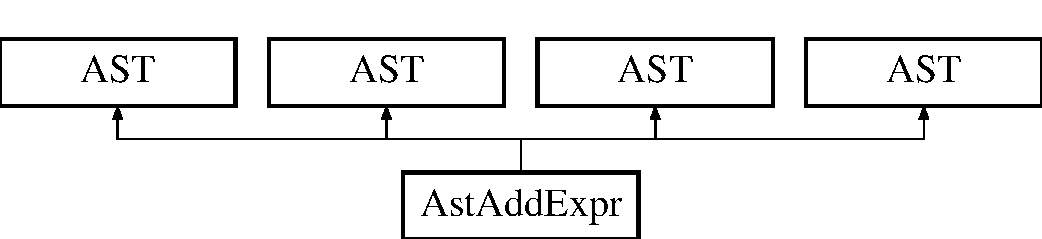
\includegraphics[height=2.000000cm]{classAstAddExpr}
\end{center}
\end{figure}
\subsection*{Public Types}
\begin{DoxyCompactItemize}
\item 
enum {\bfseries Operator} \{ \\*
{\bfseries N\-O\-N\-E}, 
{\bfseries P\-L\-U\-S}, 
{\bfseries M\-I\-N\-U\-S}, 
{\bfseries N\-O\-N\-E}, 
\\*
{\bfseries P\-L\-U\-S}, 
{\bfseries M\-I\-N\-U\-S}, 
{\bfseries N\-O\-N\-E}, 
{\bfseries P\-L\-U\-S}, 
\\*
{\bfseries M\-I\-N\-U\-S}, 
{\bfseries N\-O\-N\-E}, 
{\bfseries P\-L\-U\-S}, 
{\bfseries M\-I\-N\-U\-S}
 \}
\item 
enum {\bfseries Operator} \{ \\*
{\bfseries N\-O\-N\-E}, 
{\bfseries P\-L\-U\-S}, 
{\bfseries M\-I\-N\-U\-S}, 
{\bfseries N\-O\-N\-E}, 
\\*
{\bfseries P\-L\-U\-S}, 
{\bfseries M\-I\-N\-U\-S}, 
{\bfseries N\-O\-N\-E}, 
{\bfseries P\-L\-U\-S}, 
\\*
{\bfseries M\-I\-N\-U\-S}, 
{\bfseries N\-O\-N\-E}, 
{\bfseries P\-L\-U\-S}, 
{\bfseries M\-I\-N\-U\-S}
 \}
\item 
enum {\bfseries Operator} \{ \\*
{\bfseries N\-O\-N\-E}, 
{\bfseries P\-L\-U\-S}, 
{\bfseries M\-I\-N\-U\-S}, 
{\bfseries N\-O\-N\-E}, 
\\*
{\bfseries P\-L\-U\-S}, 
{\bfseries M\-I\-N\-U\-S}, 
{\bfseries N\-O\-N\-E}, 
{\bfseries P\-L\-U\-S}, 
\\*
{\bfseries M\-I\-N\-U\-S}, 
{\bfseries N\-O\-N\-E}, 
{\bfseries P\-L\-U\-S}, 
{\bfseries M\-I\-N\-U\-S}
 \}
\item 
enum {\bfseries Operator} \{ \\*
{\bfseries N\-O\-N\-E}, 
{\bfseries P\-L\-U\-S}, 
{\bfseries M\-I\-N\-U\-S}, 
{\bfseries N\-O\-N\-E}, 
\\*
{\bfseries P\-L\-U\-S}, 
{\bfseries M\-I\-N\-U\-S}, 
{\bfseries N\-O\-N\-E}, 
{\bfseries P\-L\-U\-S}, 
\\*
{\bfseries M\-I\-N\-U\-S}, 
{\bfseries N\-O\-N\-E}, 
{\bfseries P\-L\-U\-S}, 
{\bfseries M\-I\-N\-U\-S}
 \}
\end{DoxyCompactItemize}
\subsection*{Public Member Functions}
\begin{DoxyCompactItemize}
\item 
\hypertarget{classAstAddExpr_a62f5c5b3479834840ae3f18996354fe0}{{\bfseries Ast\-Add\-Expr} (\hyperlink{classAstMultExpr}{Ast\-Mult\-Expr} $\ast$m)}\label{classAstAddExpr_a62f5c5b3479834840ae3f18996354fe0}

\item 
\hypertarget{classAstAddExpr_a512bd2d176f23060ec0728d35ba1a492}{{\bfseries Ast\-Add\-Expr} (\hyperlink{classAstAddExpr}{Ast\-Add\-Expr} $\ast$a, Operator o, \hyperlink{classAstMultExpr}{Ast\-Mult\-Expr} $\ast$m)}\label{classAstAddExpr_a512bd2d176f23060ec0728d35ba1a492}

\item 
void \hyperlink{classAstAddExpr_a9b80132c7e2f4378ef699cd1de46fa01}{Visit} ()
\begin{DoxyCompactList}\small\item\em This function is responsible for tree traversals. \end{DoxyCompactList}\item 
\hypertarget{classAstAddExpr_a62f5c5b3479834840ae3f18996354fe0}{{\bfseries Ast\-Add\-Expr} (\hyperlink{classAstMultExpr}{Ast\-Mult\-Expr} $\ast$m)}\label{classAstAddExpr_a62f5c5b3479834840ae3f18996354fe0}

\item 
\hypertarget{classAstAddExpr_a512bd2d176f23060ec0728d35ba1a492}{{\bfseries Ast\-Add\-Expr} (\hyperlink{classAstAddExpr}{Ast\-Add\-Expr} $\ast$a, Operator o, \hyperlink{classAstMultExpr}{Ast\-Mult\-Expr} $\ast$m)}\label{classAstAddExpr_a512bd2d176f23060ec0728d35ba1a492}

\item 
void \hyperlink{classAstAddExpr_a9b80132c7e2f4378ef699cd1de46fa01}{Visit} ()
\begin{DoxyCompactList}\small\item\em This function is responsible for tree traversals. \end{DoxyCompactList}\item 
\hypertarget{classAstAddExpr_a62f5c5b3479834840ae3f18996354fe0}{{\bfseries Ast\-Add\-Expr} (\hyperlink{classAstMultExpr}{Ast\-Mult\-Expr} $\ast$m)}\label{classAstAddExpr_a62f5c5b3479834840ae3f18996354fe0}

\item 
\hypertarget{classAstAddExpr_a512bd2d176f23060ec0728d35ba1a492}{{\bfseries Ast\-Add\-Expr} (\hyperlink{classAstAddExpr}{Ast\-Add\-Expr} $\ast$a, Operator o, \hyperlink{classAstMultExpr}{Ast\-Mult\-Expr} $\ast$m)}\label{classAstAddExpr_a512bd2d176f23060ec0728d35ba1a492}

\item 
void \hyperlink{classAstAddExpr_a9b80132c7e2f4378ef699cd1de46fa01}{Visit} ()
\begin{DoxyCompactList}\small\item\em This function is responsible for tree traversals. \end{DoxyCompactList}\item 
\hypertarget{classAstAddExpr_a62f5c5b3479834840ae3f18996354fe0}{{\bfseries Ast\-Add\-Expr} (\hyperlink{classAstMultExpr}{Ast\-Mult\-Expr} $\ast$m)}\label{classAstAddExpr_a62f5c5b3479834840ae3f18996354fe0}

\item 
\hypertarget{classAstAddExpr_a512bd2d176f23060ec0728d35ba1a492}{{\bfseries Ast\-Add\-Expr} (\hyperlink{classAstAddExpr}{Ast\-Add\-Expr} $\ast$a, Operator o, \hyperlink{classAstMultExpr}{Ast\-Mult\-Expr} $\ast$m)}\label{classAstAddExpr_a512bd2d176f23060ec0728d35ba1a492}

\item 
void \hyperlink{classAstAddExpr_a9b80132c7e2f4378ef699cd1de46fa01}{Visit} ()
\begin{DoxyCompactList}\small\item\em This function is responsible for tree traversals. \end{DoxyCompactList}\item 
void \hyperlink{classAST_a71d680856e95ff89f55d5311a552eba6}{set\-Label} (string l)
\begin{DoxyCompactList}\small\item\em Sets the label for the node. \end{DoxyCompactList}\item 
void \hyperlink{classAST_a71d680856e95ff89f55d5311a552eba6}{set\-Label} (string l)
\begin{DoxyCompactList}\small\item\em Sets the label for the node. \end{DoxyCompactList}\item 
void \hyperlink{classAST_a71d680856e95ff89f55d5311a552eba6}{set\-Label} (string l)
\begin{DoxyCompactList}\small\item\em Sets the label for the node. \end{DoxyCompactList}\item 
void \hyperlink{classAST_a71d680856e95ff89f55d5311a552eba6}{set\-Label} (string l)
\begin{DoxyCompactList}\small\item\em Sets the label for the node. \end{DoxyCompactList}\item 
int \hyperlink{classAST_ab7a5b1d9f1c2de0d98deb356f724a42c}{get\-U\-I\-D} ()
\begin{DoxyCompactList}\small\item\em Gets the node's unique I\-D. \end{DoxyCompactList}\item 
int \hyperlink{classAST_ab7a5b1d9f1c2de0d98deb356f724a42c}{get\-U\-I\-D} ()
\begin{DoxyCompactList}\small\item\em Gets the node's unique I\-D. \end{DoxyCompactList}\item 
int \hyperlink{classAST_ab7a5b1d9f1c2de0d98deb356f724a42c}{get\-U\-I\-D} ()
\begin{DoxyCompactList}\small\item\em Gets the node's unique I\-D. \end{DoxyCompactList}\item 
int \hyperlink{classAST_ab7a5b1d9f1c2de0d98deb356f724a42c}{get\-U\-I\-D} ()
\begin{DoxyCompactList}\small\item\em Gets the node's unique I\-D. \end{DoxyCompactList}\item 
string \hyperlink{classAST_aee029be902fffc927d16ccb03eb922ad}{get\-Label} ()
\begin{DoxyCompactList}\small\item\em Gets the node's label. \end{DoxyCompactList}\item 
string \hyperlink{classAST_aee029be902fffc927d16ccb03eb922ad}{get\-Label} ()
\begin{DoxyCompactList}\small\item\em Gets the node's label. \end{DoxyCompactList}\item 
string \hyperlink{classAST_aee029be902fffc927d16ccb03eb922ad}{get\-Label} ()
\begin{DoxyCompactList}\small\item\em Gets the node's label. \end{DoxyCompactList}\item 
string \hyperlink{classAST_aee029be902fffc927d16ccb03eb922ad}{get\-Label} ()
\begin{DoxyCompactList}\small\item\em Gets the node's label. \end{DoxyCompactList}\end{DoxyCompactItemize}
\subsection*{Public Attributes}
\begin{DoxyCompactItemize}
\item 
\hypertarget{classAstAddExpr_aee8f2b17dced22a50fe3088795a698a6}{enum Ast\-Add\-Expr\-::\-Operator {\bfseries op}}\label{classAstAddExpr_aee8f2b17dced22a50fe3088795a698a6}

\item 
\hypertarget{classAstAddExpr_a2076082ac8b4b10910969890379f33c1}{\hyperlink{classType}{Type} $\ast$ {\bfseries type}}\label{classAstAddExpr_a2076082ac8b4b10910969890379f33c1}

\item 
\hypertarget{classAST_aaf215802de409f8096c063d01ffa6783}{bool \hyperlink{classAST_aaf215802de409f8096c063d01ffa6783}{needs\-Cast}}\label{classAST_aaf215802de409f8096c063d01ffa6783}

\begin{DoxyCompactList}\small\item\em This indicates if cast 3\-A\-C needs to be output, and is only relevant for expressions. \end{DoxyCompactList}\item 
\hypertarget{classAST_afa9e77ef650ec6664458fa6cb55be985}{bool \hyperlink{classAST_afa9e77ef650ec6664458fa6cb55be985}{is\-Conv}}\label{classAST_afa9e77ef650ec6664458fa6cb55be985}

\begin{DoxyCompactList}\small\item\em Indicates is a conversion is possible. \end{DoxyCompactList}\item 
\hypertarget{classAST_a61ef3317e023d45237e06615b387cd6b}{C\-O\-N\-V\-E\-R\-S\-I\-O\-N\-T\-Y\-P\-E \hyperlink{classAST_a61ef3317e023d45237e06615b387cd6b}{conv\-Type}}\label{classAST_a61ef3317e023d45237e06615b387cd6b}

\begin{DoxyCompactList}\small\item\em If needs\-Cast is true, then this indicates what the cast should be. \end{DoxyCompactList}\item 
\hypertarget{classAST_aea9b07b39d24183f38c0029cec0a878e}{int \hyperlink{classAST_aea9b07b39d24183f38c0029cec0a878e}{operand\-To\-Cast}}\label{classAST_aea9b07b39d24183f38c0029cec0a878e}

\begin{DoxyCompactList}\small\item\em This indicates if the first or second operand should be the one that is cast. \end{DoxyCompactList}\end{DoxyCompactItemize}
\subsection*{Static Public Attributes}
\begin{DoxyCompactItemize}
\item 
\hypertarget{classAST_a5fdfd5f7b104dd92889163bdadbc68d6}{static \hyperlink{classVisualizer}{Visualizer} \hyperlink{classAST_a5fdfd5f7b104dd92889163bdadbc68d6}{vis}}\label{classAST_a5fdfd5f7b104dd92889163bdadbc68d6}

\begin{DoxyCompactList}\small\item\em Static visualizer instance for generating the visualization of the \hyperlink{classAST}{A\-S\-T}. \end{DoxyCompactList}\item 
\hypertarget{classAST_a8a3ace322f50e030331065d644ee55ee}{static \hyperlink{classTAC__Generator}{T\-A\-C\-\_\-\-Generator} \hyperlink{classAST_a8a3ace322f50e030331065d644ee55ee}{tac\-Gen}}\label{classAST_a8a3ace322f50e030331065d644ee55ee}

\begin{DoxyCompactList}\small\item\em Three address code generator. \end{DoxyCompactList}\item 
\hypertarget{classAST_a1f69448c6dc368d005631a128460083d}{static string {\bfseries current\-Temp} =\char`\"{}\char`\"{}}\label{classAST_a1f69448c6dc368d005631a128460083d}

\item 
\hypertarget{classAST_a551aec090c932ab69365238b40a8a4eb}{static string \hyperlink{classAST_a551aec090c932ab69365238b40a8a4eb}{return\-Label} =\char`\"{}\char`\"{}}\label{classAST_a551aec090c932ab69365238b40a8a4eb}

\begin{DoxyCompactList}\small\item\em This is for storing the string id of any temporary result register that may be created during 3\-A\-C generation. \end{DoxyCompactList}\item 
\hypertarget{classAST_a73c0a266df52be71e6b527b6aa635173}{static list$<$ string $>$ {\bfseries temp\-Stack}}\label{classAST_a73c0a266df52be71e6b527b6aa635173}

\item 
\hypertarget{classAST_abf9e84b541ff04b7bb64e6e4371512d4}{static string {\bfseries last\-I\-D} =\char`\"{}\char`\"{}}\label{classAST_abf9e84b541ff04b7bb64e6e4371512d4}

\item 
\hypertarget{classAST_a163003bfe9c30510ec8039870346049f}{static \hyperlink{classSymTab}{Sym\-Tab} $\ast$ {\bfseries symbol\-Table} =N\-U\-L\-L}\label{classAST_a163003bfe9c30510ec8039870346049f}

\item 
\hypertarget{classAST_a5c3cc894d9c0453523dec9ed76f18a04}{static string {\bfseries current\-Function} =\char`\"{}\char`\"{}}\label{classAST_a5c3cc894d9c0453523dec9ed76f18a04}

\item 
\hypertarget{classAST_a66155513b59ff1a04c8ece8b20ec31f5}{static int {\bfseries current\-Constant\-Value} =0}\label{classAST_a66155513b59ff1a04c8ece8b20ec31f5}

\item 
\hypertarget{classAST_a3d031d7bab635ba1f015aade5943f40c}{static string {\bfseries current\-Id\-Name} =\char`\"{}\char`\"{}}\label{classAST_a3d031d7bab635ba1f015aade5943f40c}

\item 
\hypertarget{classAST_a16c4b6e54febc1a26b31a64a46972ef0}{static int {\bfseries current\-Index\-Val} = 0}\label{classAST_a16c4b6e54febc1a26b31a64a46972ef0}

\item 
\hypertarget{classAST_a6fc65ae9dd064a88941d4b88669b19db}{static string {\bfseries current\-I\-D} = \char`\"{}\char`\"{}}\label{classAST_a6fc65ae9dd064a88941d4b88669b19db}

\end{DoxyCompactItemize}
\subsection*{Protected Attributes}
\begin{DoxyCompactItemize}
\item 
\hypertarget{classAST_a847b778f1c3dd5a19de32de432ee6e15}{int \hyperlink{classAST_a847b778f1c3dd5a19de32de432ee6e15}{uid}}\label{classAST_a847b778f1c3dd5a19de32de432ee6e15}

\begin{DoxyCompactList}\small\item\em The unique id. \end{DoxyCompactList}\item 
\hypertarget{classAST_ab2e239ccc0688d2341724432ff5a1a31}{string \hyperlink{classAST_ab2e239ccc0688d2341724432ff5a1a31}{label}}\label{classAST_ab2e239ccc0688d2341724432ff5a1a31}

\begin{DoxyCompactList}\small\item\em The label to be printed in the visualization. \end{DoxyCompactList}\end{DoxyCompactItemize}
\subsection*{Private Attributes}
\begin{DoxyCompactItemize}
\item 
\hypertarget{classAstAddExpr_a1290fb7d961dfc6911d87803817188bb}{\hyperlink{classAstMultExpr}{Ast\-Mult\-Expr} $\ast$ {\bfseries mult}}\label{classAstAddExpr_a1290fb7d961dfc6911d87803817188bb}

\item 
\hypertarget{classAstAddExpr_a3bf1a1fdfde1ae7e4485d5048eea8cfb}{\hyperlink{classAstAddExpr}{Ast\-Add\-Expr} $\ast$ {\bfseries add}}\label{classAstAddExpr_a3bf1a1fdfde1ae7e4485d5048eea8cfb}

\end{DoxyCompactItemize}


\subsection{Detailed Description}


Definition at line 530 of file Ast.\-h.



\subsection{Member Function Documentation}
\hypertarget{classAST_aee029be902fffc927d16ccb03eb922ad}{\index{Ast\-Add\-Expr@{Ast\-Add\-Expr}!get\-Label@{get\-Label}}
\index{get\-Label@{get\-Label}!AstAddExpr@{Ast\-Add\-Expr}}
\subsubsection[{get\-Label}]{\setlength{\rightskip}{0pt plus 5cm}string A\-S\-T\-::get\-Label (
\begin{DoxyParamCaption}
{}
\end{DoxyParamCaption}
)\hspace{0.3cm}{\ttfamily [inline]}, {\ttfamily [inherited]}}}\label{classAST_aee029be902fffc927d16ccb03eb922ad}


Gets the node's label. 

\begin{DoxyReturn}{Returns}
The label 
\end{DoxyReturn}


Definition at line 60 of file Ast.\-h.

\hypertarget{classAST_aee029be902fffc927d16ccb03eb922ad}{\index{Ast\-Add\-Expr@{Ast\-Add\-Expr}!get\-Label@{get\-Label}}
\index{get\-Label@{get\-Label}!AstAddExpr@{Ast\-Add\-Expr}}
\subsubsection[{get\-Label}]{\setlength{\rightskip}{0pt plus 5cm}string A\-S\-T\-::get\-Label (
\begin{DoxyParamCaption}
{}
\end{DoxyParamCaption}
)\hspace{0.3cm}{\ttfamily [inline]}, {\ttfamily [inherited]}}}\label{classAST_aee029be902fffc927d16ccb03eb922ad}


Gets the node's label. 

\begin{DoxyReturn}{Returns}
The label 
\end{DoxyReturn}


Definition at line 60 of file C\-Scanner.\-ll.

\hypertarget{classAST_aee029be902fffc927d16ccb03eb922ad}{\index{Ast\-Add\-Expr@{Ast\-Add\-Expr}!get\-Label@{get\-Label}}
\index{get\-Label@{get\-Label}!AstAddExpr@{Ast\-Add\-Expr}}
\subsubsection[{get\-Label}]{\setlength{\rightskip}{0pt plus 5cm}string A\-S\-T\-::get\-Label (
\begin{DoxyParamCaption}
{}
\end{DoxyParamCaption}
)\hspace{0.3cm}{\ttfamily [inline]}, {\ttfamily [inherited]}}}\label{classAST_aee029be902fffc927d16ccb03eb922ad}


Gets the node's label. 

\begin{DoxyReturn}{Returns}
The label 
\end{DoxyReturn}


Definition at line 60 of file C\-Parser.\-yy.

\hypertarget{classAST_aee029be902fffc927d16ccb03eb922ad}{\index{Ast\-Add\-Expr@{Ast\-Add\-Expr}!get\-Label@{get\-Label}}
\index{get\-Label@{get\-Label}!AstAddExpr@{Ast\-Add\-Expr}}
\subsubsection[{get\-Label}]{\setlength{\rightskip}{0pt plus 5cm}string A\-S\-T\-::get\-Label (
\begin{DoxyParamCaption}
{}
\end{DoxyParamCaption}
)\hspace{0.3cm}{\ttfamily [inline]}, {\ttfamily [inherited]}}}\label{classAST_aee029be902fffc927d16ccb03eb922ad}


Gets the node's label. 

\begin{DoxyReturn}{Returns}
The label 
\end{DoxyReturn}


Definition at line 60 of file C\-Parser.\-yy.

\hypertarget{classAST_ab7a5b1d9f1c2de0d98deb356f724a42c}{\index{Ast\-Add\-Expr@{Ast\-Add\-Expr}!get\-U\-I\-D@{get\-U\-I\-D}}
\index{get\-U\-I\-D@{get\-U\-I\-D}!AstAddExpr@{Ast\-Add\-Expr}}
\subsubsection[{get\-U\-I\-D}]{\setlength{\rightskip}{0pt plus 5cm}int A\-S\-T\-::get\-U\-I\-D (
\begin{DoxyParamCaption}
{}
\end{DoxyParamCaption}
)\hspace{0.3cm}{\ttfamily [inline]}, {\ttfamily [inherited]}}}\label{classAST_ab7a5b1d9f1c2de0d98deb356f724a42c}


Gets the node's unique I\-D. 

\begin{DoxyReturn}{Returns}
The unique id 
\end{DoxyReturn}


Definition at line 53 of file C\-Parser.\-yy.

\hypertarget{classAST_ab7a5b1d9f1c2de0d98deb356f724a42c}{\index{Ast\-Add\-Expr@{Ast\-Add\-Expr}!get\-U\-I\-D@{get\-U\-I\-D}}
\index{get\-U\-I\-D@{get\-U\-I\-D}!AstAddExpr@{Ast\-Add\-Expr}}
\subsubsection[{get\-U\-I\-D}]{\setlength{\rightskip}{0pt plus 5cm}int A\-S\-T\-::get\-U\-I\-D (
\begin{DoxyParamCaption}
{}
\end{DoxyParamCaption}
)\hspace{0.3cm}{\ttfamily [inline]}, {\ttfamily [inherited]}}}\label{classAST_ab7a5b1d9f1c2de0d98deb356f724a42c}


Gets the node's unique I\-D. 

\begin{DoxyReturn}{Returns}
The unique id 
\end{DoxyReturn}


Definition at line 53 of file C\-Parser.\-yy.

\hypertarget{classAST_ab7a5b1d9f1c2de0d98deb356f724a42c}{\index{Ast\-Add\-Expr@{Ast\-Add\-Expr}!get\-U\-I\-D@{get\-U\-I\-D}}
\index{get\-U\-I\-D@{get\-U\-I\-D}!AstAddExpr@{Ast\-Add\-Expr}}
\subsubsection[{get\-U\-I\-D}]{\setlength{\rightskip}{0pt plus 5cm}int A\-S\-T\-::get\-U\-I\-D (
\begin{DoxyParamCaption}
{}
\end{DoxyParamCaption}
)\hspace{0.3cm}{\ttfamily [inline]}, {\ttfamily [inherited]}}}\label{classAST_ab7a5b1d9f1c2de0d98deb356f724a42c}


Gets the node's unique I\-D. 

\begin{DoxyReturn}{Returns}
The unique id 
\end{DoxyReturn}


Definition at line 53 of file C\-Scanner.\-ll.

\hypertarget{classAST_ab7a5b1d9f1c2de0d98deb356f724a42c}{\index{Ast\-Add\-Expr@{Ast\-Add\-Expr}!get\-U\-I\-D@{get\-U\-I\-D}}
\index{get\-U\-I\-D@{get\-U\-I\-D}!AstAddExpr@{Ast\-Add\-Expr}}
\subsubsection[{get\-U\-I\-D}]{\setlength{\rightskip}{0pt plus 5cm}int A\-S\-T\-::get\-U\-I\-D (
\begin{DoxyParamCaption}
{}
\end{DoxyParamCaption}
)\hspace{0.3cm}{\ttfamily [inline]}, {\ttfamily [inherited]}}}\label{classAST_ab7a5b1d9f1c2de0d98deb356f724a42c}


Gets the node's unique I\-D. 

\begin{DoxyReturn}{Returns}
The unique id 
\end{DoxyReturn}


Definition at line 53 of file Ast.\-h.

\hypertarget{classAST_a71d680856e95ff89f55d5311a552eba6}{\index{Ast\-Add\-Expr@{Ast\-Add\-Expr}!set\-Label@{set\-Label}}
\index{set\-Label@{set\-Label}!AstAddExpr@{Ast\-Add\-Expr}}
\subsubsection[{set\-Label}]{\setlength{\rightskip}{0pt plus 5cm}void A\-S\-T\-::set\-Label (
\begin{DoxyParamCaption}
\item[{string}]{l}
\end{DoxyParamCaption}
)\hspace{0.3cm}{\ttfamily [inline]}, {\ttfamily [inherited]}}}\label{classAST_a71d680856e95ff89f55d5311a552eba6}


Sets the label for the node. 


\begin{DoxyParams}{Parameters}
{\em l} & The label string \\
\hline
\end{DoxyParams}


Definition at line 43 of file C\-Scanner.\-ll.

\hypertarget{classAST_a71d680856e95ff89f55d5311a552eba6}{\index{Ast\-Add\-Expr@{Ast\-Add\-Expr}!set\-Label@{set\-Label}}
\index{set\-Label@{set\-Label}!AstAddExpr@{Ast\-Add\-Expr}}
\subsubsection[{set\-Label}]{\setlength{\rightskip}{0pt plus 5cm}void A\-S\-T\-::set\-Label (
\begin{DoxyParamCaption}
\item[{string}]{l}
\end{DoxyParamCaption}
)\hspace{0.3cm}{\ttfamily [inline]}, {\ttfamily [inherited]}}}\label{classAST_a71d680856e95ff89f55d5311a552eba6}


Sets the label for the node. 


\begin{DoxyParams}{Parameters}
{\em l} & The label string \\
\hline
\end{DoxyParams}


Definition at line 43 of file C\-Parser.\-yy.

\hypertarget{classAST_a71d680856e95ff89f55d5311a552eba6}{\index{Ast\-Add\-Expr@{Ast\-Add\-Expr}!set\-Label@{set\-Label}}
\index{set\-Label@{set\-Label}!AstAddExpr@{Ast\-Add\-Expr}}
\subsubsection[{set\-Label}]{\setlength{\rightskip}{0pt plus 5cm}void A\-S\-T\-::set\-Label (
\begin{DoxyParamCaption}
\item[{string}]{l}
\end{DoxyParamCaption}
)\hspace{0.3cm}{\ttfamily [inline]}, {\ttfamily [inherited]}}}\label{classAST_a71d680856e95ff89f55d5311a552eba6}


Sets the label for the node. 


\begin{DoxyParams}{Parameters}
{\em l} & The label string \\
\hline
\end{DoxyParams}


Definition at line 43 of file Ast.\-h.

\hypertarget{classAST_a71d680856e95ff89f55d5311a552eba6}{\index{Ast\-Add\-Expr@{Ast\-Add\-Expr}!set\-Label@{set\-Label}}
\index{set\-Label@{set\-Label}!AstAddExpr@{Ast\-Add\-Expr}}
\subsubsection[{set\-Label}]{\setlength{\rightskip}{0pt plus 5cm}void A\-S\-T\-::set\-Label (
\begin{DoxyParamCaption}
\item[{string}]{l}
\end{DoxyParamCaption}
)\hspace{0.3cm}{\ttfamily [inline]}, {\ttfamily [inherited]}}}\label{classAST_a71d680856e95ff89f55d5311a552eba6}


Sets the label for the node. 


\begin{DoxyParams}{Parameters}
{\em l} & The label string \\
\hline
\end{DoxyParams}


Definition at line 43 of file C\-Parser.\-yy.

\hypertarget{classAstAddExpr_a9b80132c7e2f4378ef699cd1de46fa01}{\index{Ast\-Add\-Expr@{Ast\-Add\-Expr}!Visit@{Visit}}
\index{Visit@{Visit}!AstAddExpr@{Ast\-Add\-Expr}}
\subsubsection[{Visit}]{\setlength{\rightskip}{0pt plus 5cm}void Ast\-Add\-Expr\-::\-Visit (
\begin{DoxyParamCaption}
{}
\end{DoxyParamCaption}
)\hspace{0.3cm}{\ttfamily [virtual]}}}\label{classAstAddExpr_a9b80132c7e2f4378ef699cd1de46fa01}


This function is responsible for tree traversals. 

This function will call the Visit functions of each of it's children nodes, call the visualization code for itself, and output any 3\-A\-C that can be generated at the current node. 

Reimplemented from \hyperlink{classAST_a5828cc86f2c4f1a0aeab6d7069e8fd82}{A\-S\-T}.



Definition at line 1135 of file Ast.\-cpp.

\hypertarget{classAstAddExpr_a9b80132c7e2f4378ef699cd1de46fa01}{\index{Ast\-Add\-Expr@{Ast\-Add\-Expr}!Visit@{Visit}}
\index{Visit@{Visit}!AstAddExpr@{Ast\-Add\-Expr}}
\subsubsection[{Visit}]{\setlength{\rightskip}{0pt plus 5cm}void Ast\-Add\-Expr\-::\-Visit (
\begin{DoxyParamCaption}
{}
\end{DoxyParamCaption}
)\hspace{0.3cm}{\ttfamily [virtual]}}}\label{classAstAddExpr_a9b80132c7e2f4378ef699cd1de46fa01}


This function is responsible for tree traversals. 

This function will call the Visit functions of each of it's children nodes, call the visualization code for itself, and output any 3\-A\-C that can be generated at the current node. 

Reimplemented from \hyperlink{classAST_a5828cc86f2c4f1a0aeab6d7069e8fd82}{A\-S\-T}.

\hypertarget{classAstAddExpr_a9b80132c7e2f4378ef699cd1de46fa01}{\index{Ast\-Add\-Expr@{Ast\-Add\-Expr}!Visit@{Visit}}
\index{Visit@{Visit}!AstAddExpr@{Ast\-Add\-Expr}}
\subsubsection[{Visit}]{\setlength{\rightskip}{0pt plus 5cm}void Ast\-Add\-Expr\-::\-Visit (
\begin{DoxyParamCaption}
{}
\end{DoxyParamCaption}
)\hspace{0.3cm}{\ttfamily [virtual]}}}\label{classAstAddExpr_a9b80132c7e2f4378ef699cd1de46fa01}


This function is responsible for tree traversals. 

This function will call the Visit functions of each of it's children nodes, call the visualization code for itself, and output any 3\-A\-C that can be generated at the current node. 

Reimplemented from \hyperlink{classAST_a5828cc86f2c4f1a0aeab6d7069e8fd82}{A\-S\-T}.

\hypertarget{classAstAddExpr_a9b80132c7e2f4378ef699cd1de46fa01}{\index{Ast\-Add\-Expr@{Ast\-Add\-Expr}!Visit@{Visit}}
\index{Visit@{Visit}!AstAddExpr@{Ast\-Add\-Expr}}
\subsubsection[{Visit}]{\setlength{\rightskip}{0pt plus 5cm}void Ast\-Add\-Expr\-::\-Visit (
\begin{DoxyParamCaption}
{}
\end{DoxyParamCaption}
)\hspace{0.3cm}{\ttfamily [virtual]}}}\label{classAstAddExpr_a9b80132c7e2f4378ef699cd1de46fa01}


This function is responsible for tree traversals. 

This function will call the Visit functions of each of it's children nodes, call the visualization code for itself, and output any 3\-A\-C that can be generated at the current node. 

Reimplemented from \hyperlink{classAST_a5828cc86f2c4f1a0aeab6d7069e8fd82}{A\-S\-T}.



The documentation for this class was generated from the following files\-:\begin{DoxyCompactItemize}
\item 
Ast.\-h\item 
Ast.\-cpp\end{DoxyCompactItemize}

\hypertarget{classAstAndExpr}{\section{Ast\-And\-Expr Class Reference}
\label{classAstAndExpr}\index{Ast\-And\-Expr@{Ast\-And\-Expr}}
}
Inheritance diagram for Ast\-And\-Expr\-:\begin{figure}[H]
\begin{center}
\leavevmode
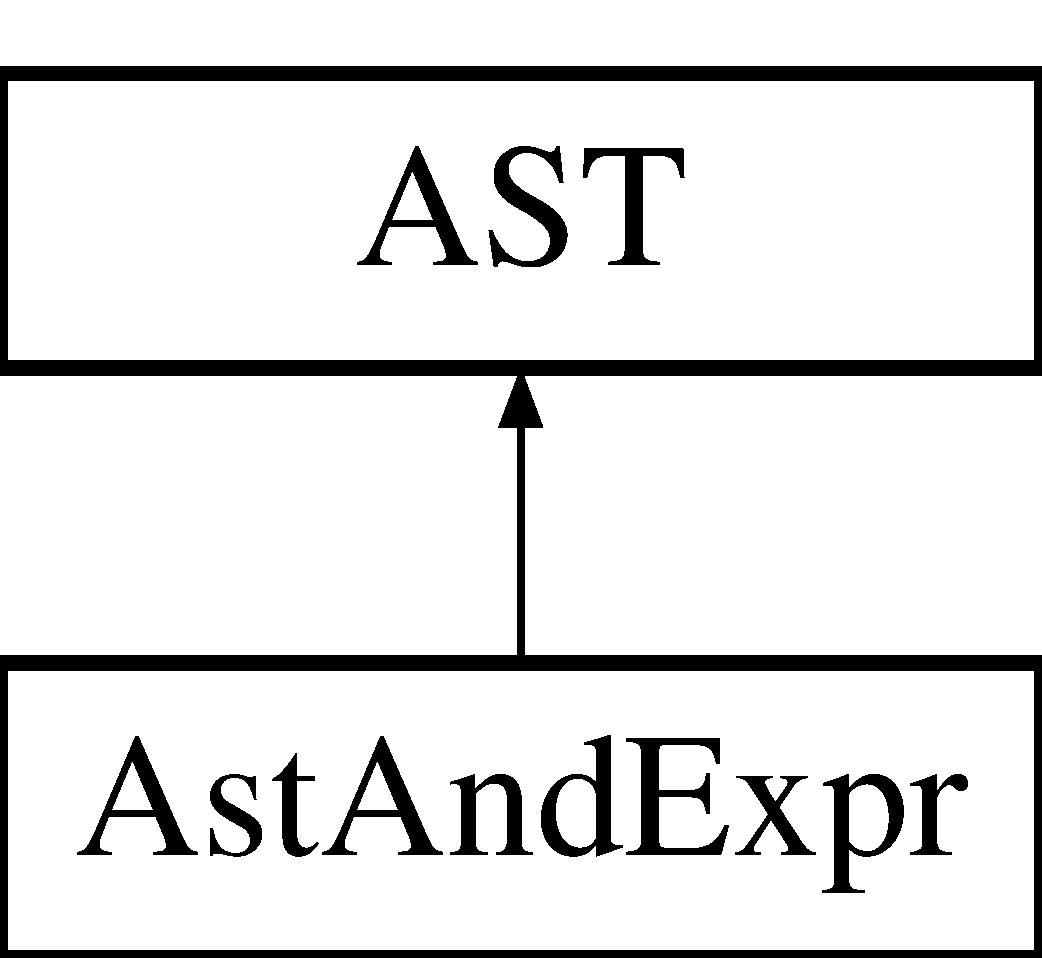
\includegraphics[height=2.000000cm]{classAstAndExpr}
\end{center}
\end{figure}
\subsection*{Public Member Functions}
\begin{DoxyCompactItemize}
\item 
\hypertarget{classAstAndExpr_ae16cf8ff39559b3e3888e37bb6c34b07}{{\bfseries Ast\-And\-Expr} (\hyperlink{classAstEqExpr}{Ast\-Eq\-Expr} $\ast$e)}\label{classAstAndExpr_ae16cf8ff39559b3e3888e37bb6c34b07}

\item 
\hypertarget{classAstAndExpr_ace64f90b89de62e5099b3cf1a853972e}{{\bfseries Ast\-And\-Expr} (\hyperlink{classAstAndExpr}{Ast\-And\-Expr} $\ast$a, \hyperlink{classAstEqExpr}{Ast\-Eq\-Expr} $\ast$e)}\label{classAstAndExpr_ace64f90b89de62e5099b3cf1a853972e}

\item 
\hypertarget{classAstAndExpr_a0d5cb855afb4a400c2c1a8cda617cf9b}{void {\bfseries Visit} ()}\label{classAstAndExpr_a0d5cb855afb4a400c2c1a8cda617cf9b}

\item 
\hypertarget{classAST_a71d680856e95ff89f55d5311a552eba6}{void {\bfseries set\-Label} (string l)}\label{classAST_a71d680856e95ff89f55d5311a552eba6}

\item 
\hypertarget{classAST_ab7a5b1d9f1c2de0d98deb356f724a42c}{int {\bfseries get\-U\-I\-D} ()}\label{classAST_ab7a5b1d9f1c2de0d98deb356f724a42c}

\item 
\hypertarget{classAST_aee029be902fffc927d16ccb03eb922ad}{string {\bfseries get\-Label} ()}\label{classAST_aee029be902fffc927d16ccb03eb922ad}

\end{DoxyCompactItemize}
\subsection*{Static Public Attributes}
\begin{DoxyCompactItemize}
\item 
\hypertarget{classAST_aca9e6637209b31e03a09c0d42f29bdfa}{static \hyperlink{classVisualizer}{Visualizer} {\bfseries vis}}\label{classAST_aca9e6637209b31e03a09c0d42f29bdfa}

\end{DoxyCompactItemize}
\subsection*{Protected Attributes}
\begin{DoxyCompactItemize}
\item 
\hypertarget{classAST_a847b778f1c3dd5a19de32de432ee6e15}{int {\bfseries uid}}\label{classAST_a847b778f1c3dd5a19de32de432ee6e15}

\item 
\hypertarget{classAST_ab2e239ccc0688d2341724432ff5a1a31}{string {\bfseries label}}\label{classAST_ab2e239ccc0688d2341724432ff5a1a31}

\end{DoxyCompactItemize}
\subsection*{Private Attributes}
\begin{DoxyCompactItemize}
\item 
\hypertarget{classAstAndExpr_aec33f836a7d0f47cf78bc11043935313}{\hyperlink{classAstEqExpr}{Ast\-Eq\-Expr} $\ast$ {\bfseries eq}}\label{classAstAndExpr_aec33f836a7d0f47cf78bc11043935313}

\item 
\hypertarget{classAstAndExpr_ab9f16e8ea62625a5d66792a08b6a3ae2}{\hyperlink{classAstAndExpr}{Ast\-And\-Expr} $\ast$ {\bfseries a}}\label{classAstAndExpr_ab9f16e8ea62625a5d66792a08b6a3ae2}

\end{DoxyCompactItemize}


The documentation for this class was generated from the following files\-:\begin{DoxyCompactItemize}
\item 
Ast.\-h\item 
Ast.\-cpp\end{DoxyCompactItemize}

\hypertarget{classAstArgExprList}{\section{Ast\-Arg\-Expr\-List Class Reference}
\label{classAstArgExprList}\index{Ast\-Arg\-Expr\-List@{Ast\-Arg\-Expr\-List}}
}
Inheritance diagram for Ast\-Arg\-Expr\-List\-:\begin{figure}[H]
\begin{center}
\leavevmode
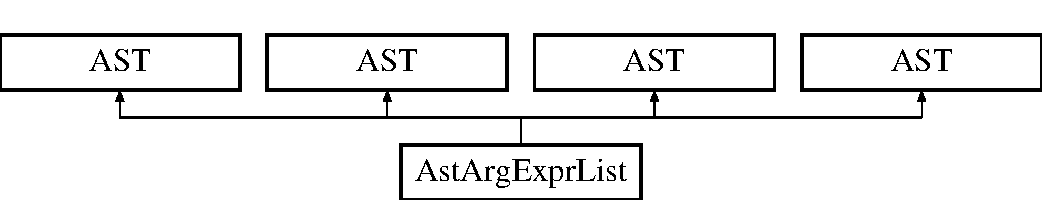
\includegraphics[height=2.000000cm]{classAstArgExprList}
\end{center}
\end{figure}
\subsection*{Public Member Functions}
\begin{DoxyCompactItemize}
\item 
\hypertarget{classAstArgExprList_a6aafae6eaadd5db52a33768136657610}{{\bfseries Ast\-Arg\-Expr\-List} (\hyperlink{classAstArgExprList}{Ast\-Arg\-Expr\-List} $\ast$list, \hyperlink{classAstAssignExpr}{Ast\-Assign\-Expr} $\ast$expr)}\label{classAstArgExprList_a6aafae6eaadd5db52a33768136657610}

\item 
\hypertarget{classAstArgExprList_a4acc4d03bbbe66b9a19e991d21169414}{{\bfseries Ast\-Arg\-Expr\-List} (\hyperlink{classAstAssignExpr}{Ast\-Assign\-Expr} $\ast$expr)}\label{classAstArgExprList_a4acc4d03bbbe66b9a19e991d21169414}

\item 
void \hyperlink{classAstArgExprList_aeac192a90197b0de59114cea84a1e577}{Visit} ()
\begin{DoxyCompactList}\small\item\em This function is responsible for tree traversals. \end{DoxyCompactList}\item 
\hypertarget{classAstArgExprList_a6aafae6eaadd5db52a33768136657610}{{\bfseries Ast\-Arg\-Expr\-List} (\hyperlink{classAstArgExprList}{Ast\-Arg\-Expr\-List} $\ast$list, \hyperlink{classAstAssignExpr}{Ast\-Assign\-Expr} $\ast$expr)}\label{classAstArgExprList_a6aafae6eaadd5db52a33768136657610}

\item 
\hypertarget{classAstArgExprList_a4acc4d03bbbe66b9a19e991d21169414}{{\bfseries Ast\-Arg\-Expr\-List} (\hyperlink{classAstAssignExpr}{Ast\-Assign\-Expr} $\ast$expr)}\label{classAstArgExprList_a4acc4d03bbbe66b9a19e991d21169414}

\item 
void \hyperlink{classAstArgExprList_aeac192a90197b0de59114cea84a1e577}{Visit} ()
\begin{DoxyCompactList}\small\item\em This function is responsible for tree traversals. \end{DoxyCompactList}\item 
\hypertarget{classAstArgExprList_a6aafae6eaadd5db52a33768136657610}{{\bfseries Ast\-Arg\-Expr\-List} (\hyperlink{classAstArgExprList}{Ast\-Arg\-Expr\-List} $\ast$list, \hyperlink{classAstAssignExpr}{Ast\-Assign\-Expr} $\ast$expr)}\label{classAstArgExprList_a6aafae6eaadd5db52a33768136657610}

\item 
\hypertarget{classAstArgExprList_a4acc4d03bbbe66b9a19e991d21169414}{{\bfseries Ast\-Arg\-Expr\-List} (\hyperlink{classAstAssignExpr}{Ast\-Assign\-Expr} $\ast$expr)}\label{classAstArgExprList_a4acc4d03bbbe66b9a19e991d21169414}

\item 
void \hyperlink{classAstArgExprList_aeac192a90197b0de59114cea84a1e577}{Visit} ()
\begin{DoxyCompactList}\small\item\em This function is responsible for tree traversals. \end{DoxyCompactList}\item 
\hypertarget{classAstArgExprList_a6aafae6eaadd5db52a33768136657610}{{\bfseries Ast\-Arg\-Expr\-List} (\hyperlink{classAstArgExprList}{Ast\-Arg\-Expr\-List} $\ast$list, \hyperlink{classAstAssignExpr}{Ast\-Assign\-Expr} $\ast$expr)}\label{classAstArgExprList_a6aafae6eaadd5db52a33768136657610}

\item 
\hypertarget{classAstArgExprList_a4acc4d03bbbe66b9a19e991d21169414}{{\bfseries Ast\-Arg\-Expr\-List} (\hyperlink{classAstAssignExpr}{Ast\-Assign\-Expr} $\ast$expr)}\label{classAstArgExprList_a4acc4d03bbbe66b9a19e991d21169414}

\item 
void \hyperlink{classAstArgExprList_aeac192a90197b0de59114cea84a1e577}{Visit} ()
\begin{DoxyCompactList}\small\item\em This function is responsible for tree traversals. \end{DoxyCompactList}\item 
void \hyperlink{classAST_a71d680856e95ff89f55d5311a552eba6}{set\-Label} (string l)
\begin{DoxyCompactList}\small\item\em Sets the label for the node. \end{DoxyCompactList}\item 
void \hyperlink{classAST_a71d680856e95ff89f55d5311a552eba6}{set\-Label} (string l)
\begin{DoxyCompactList}\small\item\em Sets the label for the node. \end{DoxyCompactList}\item 
void \hyperlink{classAST_a71d680856e95ff89f55d5311a552eba6}{set\-Label} (string l)
\begin{DoxyCompactList}\small\item\em Sets the label for the node. \end{DoxyCompactList}\item 
void \hyperlink{classAST_a71d680856e95ff89f55d5311a552eba6}{set\-Label} (string l)
\begin{DoxyCompactList}\small\item\em Sets the label for the node. \end{DoxyCompactList}\item 
int \hyperlink{classAST_ab7a5b1d9f1c2de0d98deb356f724a42c}{get\-U\-I\-D} ()
\begin{DoxyCompactList}\small\item\em Gets the node's unique I\-D. \end{DoxyCompactList}\item 
int \hyperlink{classAST_ab7a5b1d9f1c2de0d98deb356f724a42c}{get\-U\-I\-D} ()
\begin{DoxyCompactList}\small\item\em Gets the node's unique I\-D. \end{DoxyCompactList}\item 
int \hyperlink{classAST_ab7a5b1d9f1c2de0d98deb356f724a42c}{get\-U\-I\-D} ()
\begin{DoxyCompactList}\small\item\em Gets the node's unique I\-D. \end{DoxyCompactList}\item 
int \hyperlink{classAST_ab7a5b1d9f1c2de0d98deb356f724a42c}{get\-U\-I\-D} ()
\begin{DoxyCompactList}\small\item\em Gets the node's unique I\-D. \end{DoxyCompactList}\item 
string \hyperlink{classAST_aee029be902fffc927d16ccb03eb922ad}{get\-Label} ()
\begin{DoxyCompactList}\small\item\em Gets the node's label. \end{DoxyCompactList}\item 
string \hyperlink{classAST_aee029be902fffc927d16ccb03eb922ad}{get\-Label} ()
\begin{DoxyCompactList}\small\item\em Gets the node's label. \end{DoxyCompactList}\item 
string \hyperlink{classAST_aee029be902fffc927d16ccb03eb922ad}{get\-Label} ()
\begin{DoxyCompactList}\small\item\em Gets the node's label. \end{DoxyCompactList}\item 
string \hyperlink{classAST_aee029be902fffc927d16ccb03eb922ad}{get\-Label} ()
\begin{DoxyCompactList}\small\item\em Gets the node's label. \end{DoxyCompactList}\end{DoxyCompactItemize}
\subsection*{Public Attributes}
\begin{DoxyCompactItemize}
\item 
\hypertarget{classAST_aaf215802de409f8096c063d01ffa6783}{bool \hyperlink{classAST_aaf215802de409f8096c063d01ffa6783}{needs\-Cast}}\label{classAST_aaf215802de409f8096c063d01ffa6783}

\begin{DoxyCompactList}\small\item\em This indicates if cast 3\-A\-C needs to be output, and is only relevant for expressions. \end{DoxyCompactList}\item 
\hypertarget{classAST_afa9e77ef650ec6664458fa6cb55be985}{bool \hyperlink{classAST_afa9e77ef650ec6664458fa6cb55be985}{is\-Conv}}\label{classAST_afa9e77ef650ec6664458fa6cb55be985}

\begin{DoxyCompactList}\small\item\em Indicates is a conversion is possible. \end{DoxyCompactList}\item 
\hypertarget{classAST_a61ef3317e023d45237e06615b387cd6b}{C\-O\-N\-V\-E\-R\-S\-I\-O\-N\-T\-Y\-P\-E \hyperlink{classAST_a61ef3317e023d45237e06615b387cd6b}{conv\-Type}}\label{classAST_a61ef3317e023d45237e06615b387cd6b}

\begin{DoxyCompactList}\small\item\em If needs\-Cast is true, then this indicates what the cast should be. \end{DoxyCompactList}\item 
\hypertarget{classAST_aea9b07b39d24183f38c0029cec0a878e}{int \hyperlink{classAST_aea9b07b39d24183f38c0029cec0a878e}{operand\-To\-Cast}}\label{classAST_aea9b07b39d24183f38c0029cec0a878e}

\begin{DoxyCompactList}\small\item\em This indicates if the first or second operand should be the one that is cast. \end{DoxyCompactList}\end{DoxyCompactItemize}
\subsection*{Static Public Attributes}
\begin{DoxyCompactItemize}
\item 
\hypertarget{classAST_a5fdfd5f7b104dd92889163bdadbc68d6}{static \hyperlink{classVisualizer}{Visualizer} \hyperlink{classAST_a5fdfd5f7b104dd92889163bdadbc68d6}{vis}}\label{classAST_a5fdfd5f7b104dd92889163bdadbc68d6}

\begin{DoxyCompactList}\small\item\em Static visualizer instance for generating the visualization of the \hyperlink{classAST}{A\-S\-T}. \end{DoxyCompactList}\item 
\hypertarget{classAST_a8a3ace322f50e030331065d644ee55ee}{static \hyperlink{classTAC__Generator}{T\-A\-C\-\_\-\-Generator} \hyperlink{classAST_a8a3ace322f50e030331065d644ee55ee}{tac\-Gen}}\label{classAST_a8a3ace322f50e030331065d644ee55ee}

\begin{DoxyCompactList}\small\item\em Three address code generator. \end{DoxyCompactList}\item 
\hypertarget{classAST_a1f69448c6dc368d005631a128460083d}{static string {\bfseries current\-Temp} =\char`\"{}\char`\"{}}\label{classAST_a1f69448c6dc368d005631a128460083d}

\item 
\hypertarget{classAST_a551aec090c932ab69365238b40a8a4eb}{static string \hyperlink{classAST_a551aec090c932ab69365238b40a8a4eb}{return\-Label} =\char`\"{}\char`\"{}}\label{classAST_a551aec090c932ab69365238b40a8a4eb}

\begin{DoxyCompactList}\small\item\em This is for storing the string id of any temporary result register that may be created during 3\-A\-C generation. \end{DoxyCompactList}\item 
\hypertarget{classAST_a73c0a266df52be71e6b527b6aa635173}{static list$<$ string $>$ {\bfseries temp\-Stack}}\label{classAST_a73c0a266df52be71e6b527b6aa635173}

\item 
\hypertarget{classAST_abf9e84b541ff04b7bb64e6e4371512d4}{static string {\bfseries last\-I\-D} =\char`\"{}\char`\"{}}\label{classAST_abf9e84b541ff04b7bb64e6e4371512d4}

\item 
\hypertarget{classAST_a163003bfe9c30510ec8039870346049f}{static \hyperlink{classSymTab}{Sym\-Tab} $\ast$ {\bfseries symbol\-Table} =N\-U\-L\-L}\label{classAST_a163003bfe9c30510ec8039870346049f}

\item 
\hypertarget{classAST_a5c3cc894d9c0453523dec9ed76f18a04}{static string {\bfseries current\-Function} =\char`\"{}\char`\"{}}\label{classAST_a5c3cc894d9c0453523dec9ed76f18a04}

\end{DoxyCompactItemize}
\subsection*{Protected Attributes}
\begin{DoxyCompactItemize}
\item 
\hypertarget{classAST_a847b778f1c3dd5a19de32de432ee6e15}{int \hyperlink{classAST_a847b778f1c3dd5a19de32de432ee6e15}{uid}}\label{classAST_a847b778f1c3dd5a19de32de432ee6e15}

\begin{DoxyCompactList}\small\item\em The unique id. \end{DoxyCompactList}\item 
\hypertarget{classAST_ab2e239ccc0688d2341724432ff5a1a31}{string \hyperlink{classAST_ab2e239ccc0688d2341724432ff5a1a31}{label}}\label{classAST_ab2e239ccc0688d2341724432ff5a1a31}

\begin{DoxyCompactList}\small\item\em The label to be printed in the visualization. \end{DoxyCompactList}\end{DoxyCompactItemize}
\subsection*{Private Attributes}
\begin{DoxyCompactItemize}
\item 
\hypertarget{classAstArgExprList_a09c2206919e81a26cdcfacc751975418}{\hyperlink{classAstArgExprList}{Ast\-Arg\-Expr\-List} $\ast$ {\bfseries list}}\label{classAstArgExprList_a09c2206919e81a26cdcfacc751975418}

\item 
\hypertarget{classAstArgExprList_a3548a100512513833a239240af0ad311}{\hyperlink{classAstAssignExpr}{Ast\-Assign\-Expr} $\ast$ {\bfseries expr}}\label{classAstArgExprList_a3548a100512513833a239240af0ad311}

\item 
\hypertarget{classAstArgExprList_a38260d038461e9bad44d41cc7f663c52}{bool {\bfseries is\-Last\-Item}}\label{classAstArgExprList_a38260d038461e9bad44d41cc7f663c52}

\end{DoxyCompactItemize}


\subsection{Detailed Description}


Definition at line 242 of file Ast.\-h.



\subsection{Member Function Documentation}
\hypertarget{classAST_aee029be902fffc927d16ccb03eb922ad}{\index{Ast\-Arg\-Expr\-List@{Ast\-Arg\-Expr\-List}!get\-Label@{get\-Label}}
\index{get\-Label@{get\-Label}!AstArgExprList@{Ast\-Arg\-Expr\-List}}
\subsubsection[{get\-Label}]{\setlength{\rightskip}{0pt plus 5cm}string A\-S\-T\-::get\-Label (
\begin{DoxyParamCaption}
{}
\end{DoxyParamCaption}
)\hspace{0.3cm}{\ttfamily [inline]}, {\ttfamily [inherited]}}}\label{classAST_aee029be902fffc927d16ccb03eb922ad}


Gets the node's label. 

\begin{DoxyReturn}{Returns}
The label 
\end{DoxyReturn}


Definition at line 60 of file Ast.\-h.

\hypertarget{classAST_aee029be902fffc927d16ccb03eb922ad}{\index{Ast\-Arg\-Expr\-List@{Ast\-Arg\-Expr\-List}!get\-Label@{get\-Label}}
\index{get\-Label@{get\-Label}!AstArgExprList@{Ast\-Arg\-Expr\-List}}
\subsubsection[{get\-Label}]{\setlength{\rightskip}{0pt plus 5cm}string A\-S\-T\-::get\-Label (
\begin{DoxyParamCaption}
{}
\end{DoxyParamCaption}
)\hspace{0.3cm}{\ttfamily [inline]}, {\ttfamily [inherited]}}}\label{classAST_aee029be902fffc927d16ccb03eb922ad}


Gets the node's label. 

\begin{DoxyReturn}{Returns}
The label 
\end{DoxyReturn}


Definition at line 60 of file C\-Scanner.\-ll.

\hypertarget{classAST_aee029be902fffc927d16ccb03eb922ad}{\index{Ast\-Arg\-Expr\-List@{Ast\-Arg\-Expr\-List}!get\-Label@{get\-Label}}
\index{get\-Label@{get\-Label}!AstArgExprList@{Ast\-Arg\-Expr\-List}}
\subsubsection[{get\-Label}]{\setlength{\rightskip}{0pt plus 5cm}string A\-S\-T\-::get\-Label (
\begin{DoxyParamCaption}
{}
\end{DoxyParamCaption}
)\hspace{0.3cm}{\ttfamily [inline]}, {\ttfamily [inherited]}}}\label{classAST_aee029be902fffc927d16ccb03eb922ad}


Gets the node's label. 

\begin{DoxyReturn}{Returns}
The label 
\end{DoxyReturn}


Definition at line 60 of file C\-Parser.\-yy.

\hypertarget{classAST_aee029be902fffc927d16ccb03eb922ad}{\index{Ast\-Arg\-Expr\-List@{Ast\-Arg\-Expr\-List}!get\-Label@{get\-Label}}
\index{get\-Label@{get\-Label}!AstArgExprList@{Ast\-Arg\-Expr\-List}}
\subsubsection[{get\-Label}]{\setlength{\rightskip}{0pt plus 5cm}string A\-S\-T\-::get\-Label (
\begin{DoxyParamCaption}
{}
\end{DoxyParamCaption}
)\hspace{0.3cm}{\ttfamily [inline]}, {\ttfamily [inherited]}}}\label{classAST_aee029be902fffc927d16ccb03eb922ad}


Gets the node's label. 

\begin{DoxyReturn}{Returns}
The label 
\end{DoxyReturn}


Definition at line 60 of file C\-Parser.\-yy.

\hypertarget{classAST_ab7a5b1d9f1c2de0d98deb356f724a42c}{\index{Ast\-Arg\-Expr\-List@{Ast\-Arg\-Expr\-List}!get\-U\-I\-D@{get\-U\-I\-D}}
\index{get\-U\-I\-D@{get\-U\-I\-D}!AstArgExprList@{Ast\-Arg\-Expr\-List}}
\subsubsection[{get\-U\-I\-D}]{\setlength{\rightskip}{0pt plus 5cm}int A\-S\-T\-::get\-U\-I\-D (
\begin{DoxyParamCaption}
{}
\end{DoxyParamCaption}
)\hspace{0.3cm}{\ttfamily [inline]}, {\ttfamily [inherited]}}}\label{classAST_ab7a5b1d9f1c2de0d98deb356f724a42c}


Gets the node's unique I\-D. 

\begin{DoxyReturn}{Returns}
The unique id 
\end{DoxyReturn}


Definition at line 53 of file C\-Parser.\-yy.

\hypertarget{classAST_ab7a5b1d9f1c2de0d98deb356f724a42c}{\index{Ast\-Arg\-Expr\-List@{Ast\-Arg\-Expr\-List}!get\-U\-I\-D@{get\-U\-I\-D}}
\index{get\-U\-I\-D@{get\-U\-I\-D}!AstArgExprList@{Ast\-Arg\-Expr\-List}}
\subsubsection[{get\-U\-I\-D}]{\setlength{\rightskip}{0pt plus 5cm}int A\-S\-T\-::get\-U\-I\-D (
\begin{DoxyParamCaption}
{}
\end{DoxyParamCaption}
)\hspace{0.3cm}{\ttfamily [inline]}, {\ttfamily [inherited]}}}\label{classAST_ab7a5b1d9f1c2de0d98deb356f724a42c}


Gets the node's unique I\-D. 

\begin{DoxyReturn}{Returns}
The unique id 
\end{DoxyReturn}


Definition at line 53 of file C\-Parser.\-yy.

\hypertarget{classAST_ab7a5b1d9f1c2de0d98deb356f724a42c}{\index{Ast\-Arg\-Expr\-List@{Ast\-Arg\-Expr\-List}!get\-U\-I\-D@{get\-U\-I\-D}}
\index{get\-U\-I\-D@{get\-U\-I\-D}!AstArgExprList@{Ast\-Arg\-Expr\-List}}
\subsubsection[{get\-U\-I\-D}]{\setlength{\rightskip}{0pt plus 5cm}int A\-S\-T\-::get\-U\-I\-D (
\begin{DoxyParamCaption}
{}
\end{DoxyParamCaption}
)\hspace{0.3cm}{\ttfamily [inline]}, {\ttfamily [inherited]}}}\label{classAST_ab7a5b1d9f1c2de0d98deb356f724a42c}


Gets the node's unique I\-D. 

\begin{DoxyReturn}{Returns}
The unique id 
\end{DoxyReturn}


Definition at line 53 of file C\-Scanner.\-ll.

\hypertarget{classAST_ab7a5b1d9f1c2de0d98deb356f724a42c}{\index{Ast\-Arg\-Expr\-List@{Ast\-Arg\-Expr\-List}!get\-U\-I\-D@{get\-U\-I\-D}}
\index{get\-U\-I\-D@{get\-U\-I\-D}!AstArgExprList@{Ast\-Arg\-Expr\-List}}
\subsubsection[{get\-U\-I\-D}]{\setlength{\rightskip}{0pt plus 5cm}int A\-S\-T\-::get\-U\-I\-D (
\begin{DoxyParamCaption}
{}
\end{DoxyParamCaption}
)\hspace{0.3cm}{\ttfamily [inline]}, {\ttfamily [inherited]}}}\label{classAST_ab7a5b1d9f1c2de0d98deb356f724a42c}


Gets the node's unique I\-D. 

\begin{DoxyReturn}{Returns}
The unique id 
\end{DoxyReturn}


Definition at line 53 of file Ast.\-h.

\hypertarget{classAST_a71d680856e95ff89f55d5311a552eba6}{\index{Ast\-Arg\-Expr\-List@{Ast\-Arg\-Expr\-List}!set\-Label@{set\-Label}}
\index{set\-Label@{set\-Label}!AstArgExprList@{Ast\-Arg\-Expr\-List}}
\subsubsection[{set\-Label}]{\setlength{\rightskip}{0pt plus 5cm}void A\-S\-T\-::set\-Label (
\begin{DoxyParamCaption}
\item[{string}]{l}
\end{DoxyParamCaption}
)\hspace{0.3cm}{\ttfamily [inline]}, {\ttfamily [inherited]}}}\label{classAST_a71d680856e95ff89f55d5311a552eba6}


Sets the label for the node. 


\begin{DoxyParams}{Parameters}
{\em l} & The label string \\
\hline
\end{DoxyParams}


Definition at line 43 of file C\-Scanner.\-ll.

\hypertarget{classAST_a71d680856e95ff89f55d5311a552eba6}{\index{Ast\-Arg\-Expr\-List@{Ast\-Arg\-Expr\-List}!set\-Label@{set\-Label}}
\index{set\-Label@{set\-Label}!AstArgExprList@{Ast\-Arg\-Expr\-List}}
\subsubsection[{set\-Label}]{\setlength{\rightskip}{0pt plus 5cm}void A\-S\-T\-::set\-Label (
\begin{DoxyParamCaption}
\item[{string}]{l}
\end{DoxyParamCaption}
)\hspace{0.3cm}{\ttfamily [inline]}, {\ttfamily [inherited]}}}\label{classAST_a71d680856e95ff89f55d5311a552eba6}


Sets the label for the node. 


\begin{DoxyParams}{Parameters}
{\em l} & The label string \\
\hline
\end{DoxyParams}


Definition at line 43 of file C\-Parser.\-yy.

\hypertarget{classAST_a71d680856e95ff89f55d5311a552eba6}{\index{Ast\-Arg\-Expr\-List@{Ast\-Arg\-Expr\-List}!set\-Label@{set\-Label}}
\index{set\-Label@{set\-Label}!AstArgExprList@{Ast\-Arg\-Expr\-List}}
\subsubsection[{set\-Label}]{\setlength{\rightskip}{0pt plus 5cm}void A\-S\-T\-::set\-Label (
\begin{DoxyParamCaption}
\item[{string}]{l}
\end{DoxyParamCaption}
)\hspace{0.3cm}{\ttfamily [inline]}, {\ttfamily [inherited]}}}\label{classAST_a71d680856e95ff89f55d5311a552eba6}


Sets the label for the node. 


\begin{DoxyParams}{Parameters}
{\em l} & The label string \\
\hline
\end{DoxyParams}


Definition at line 43 of file Ast.\-h.

\hypertarget{classAST_a71d680856e95ff89f55d5311a552eba6}{\index{Ast\-Arg\-Expr\-List@{Ast\-Arg\-Expr\-List}!set\-Label@{set\-Label}}
\index{set\-Label@{set\-Label}!AstArgExprList@{Ast\-Arg\-Expr\-List}}
\subsubsection[{set\-Label}]{\setlength{\rightskip}{0pt plus 5cm}void A\-S\-T\-::set\-Label (
\begin{DoxyParamCaption}
\item[{string}]{l}
\end{DoxyParamCaption}
)\hspace{0.3cm}{\ttfamily [inline]}, {\ttfamily [inherited]}}}\label{classAST_a71d680856e95ff89f55d5311a552eba6}


Sets the label for the node. 


\begin{DoxyParams}{Parameters}
{\em l} & The label string \\
\hline
\end{DoxyParams}


Definition at line 43 of file C\-Parser.\-yy.

\hypertarget{classAstArgExprList_aeac192a90197b0de59114cea84a1e577}{\index{Ast\-Arg\-Expr\-List@{Ast\-Arg\-Expr\-List}!Visit@{Visit}}
\index{Visit@{Visit}!AstArgExprList@{Ast\-Arg\-Expr\-List}}
\subsubsection[{Visit}]{\setlength{\rightskip}{0pt plus 5cm}void Ast\-Arg\-Expr\-List\-::\-Visit (
\begin{DoxyParamCaption}
{}
\end{DoxyParamCaption}
)\hspace{0.3cm}{\ttfamily [virtual]}}}\label{classAstArgExprList_aeac192a90197b0de59114cea84a1e577}


This function is responsible for tree traversals. 

This function will call the Visit functions of each of it's children nodes, call the visualization code for itself, and output any 3\-A\-C that can be generated at the current node. 

Reimplemented from \hyperlink{classAST_a5828cc86f2c4f1a0aeab6d7069e8fd82}{A\-S\-T}.



Definition at line 145 of file Ast.\-cpp.

\hypertarget{classAstArgExprList_aeac192a90197b0de59114cea84a1e577}{\index{Ast\-Arg\-Expr\-List@{Ast\-Arg\-Expr\-List}!Visit@{Visit}}
\index{Visit@{Visit}!AstArgExprList@{Ast\-Arg\-Expr\-List}}
\subsubsection[{Visit}]{\setlength{\rightskip}{0pt plus 5cm}void Ast\-Arg\-Expr\-List\-::\-Visit (
\begin{DoxyParamCaption}
{}
\end{DoxyParamCaption}
)\hspace{0.3cm}{\ttfamily [virtual]}}}\label{classAstArgExprList_aeac192a90197b0de59114cea84a1e577}


This function is responsible for tree traversals. 

This function will call the Visit functions of each of it's children nodes, call the visualization code for itself, and output any 3\-A\-C that can be generated at the current node. 

Reimplemented from \hyperlink{classAST_a5828cc86f2c4f1a0aeab6d7069e8fd82}{A\-S\-T}.

\hypertarget{classAstArgExprList_aeac192a90197b0de59114cea84a1e577}{\index{Ast\-Arg\-Expr\-List@{Ast\-Arg\-Expr\-List}!Visit@{Visit}}
\index{Visit@{Visit}!AstArgExprList@{Ast\-Arg\-Expr\-List}}
\subsubsection[{Visit}]{\setlength{\rightskip}{0pt plus 5cm}void Ast\-Arg\-Expr\-List\-::\-Visit (
\begin{DoxyParamCaption}
{}
\end{DoxyParamCaption}
)\hspace{0.3cm}{\ttfamily [virtual]}}}\label{classAstArgExprList_aeac192a90197b0de59114cea84a1e577}


This function is responsible for tree traversals. 

This function will call the Visit functions of each of it's children nodes, call the visualization code for itself, and output any 3\-A\-C that can be generated at the current node. 

Reimplemented from \hyperlink{classAST_a5828cc86f2c4f1a0aeab6d7069e8fd82}{A\-S\-T}.

\hypertarget{classAstArgExprList_aeac192a90197b0de59114cea84a1e577}{\index{Ast\-Arg\-Expr\-List@{Ast\-Arg\-Expr\-List}!Visit@{Visit}}
\index{Visit@{Visit}!AstArgExprList@{Ast\-Arg\-Expr\-List}}
\subsubsection[{Visit}]{\setlength{\rightskip}{0pt plus 5cm}void Ast\-Arg\-Expr\-List\-::\-Visit (
\begin{DoxyParamCaption}
{}
\end{DoxyParamCaption}
)\hspace{0.3cm}{\ttfamily [virtual]}}}\label{classAstArgExprList_aeac192a90197b0de59114cea84a1e577}


This function is responsible for tree traversals. 

This function will call the Visit functions of each of it's children nodes, call the visualization code for itself, and output any 3\-A\-C that can be generated at the current node. 

Reimplemented from \hyperlink{classAST_a5828cc86f2c4f1a0aeab6d7069e8fd82}{A\-S\-T}.



The documentation for this class was generated from the following files\-:\begin{DoxyCompactItemize}
\item 
Ast.\-h\item 
Ast.\-cpp\end{DoxyCompactItemize}

\hypertarget{classAstAssignExpr}{\section{Ast\-Assign\-Expr Class Reference}
\label{classAstAssignExpr}\index{Ast\-Assign\-Expr@{Ast\-Assign\-Expr}}
}
Inheritance diagram for Ast\-Assign\-Expr\-:\begin{figure}[H]
\begin{center}
\leavevmode
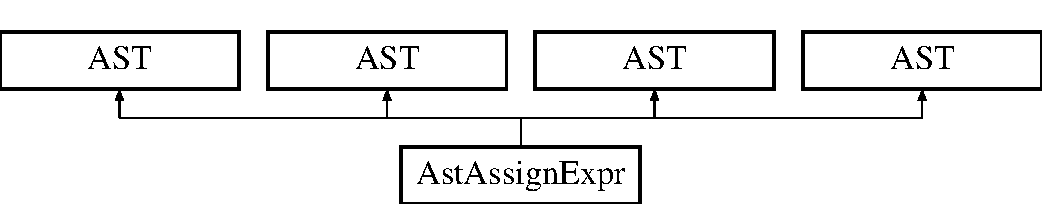
\includegraphics[height=2.000000cm]{classAstAssignExpr}
\end{center}
\end{figure}
\subsection*{Public Member Functions}
\begin{DoxyCompactItemize}
\item 
\hypertarget{classAstAssignExpr_adcf8fd9d2e80a579e8fad5ae28c79211}{{\bfseries Ast\-Assign\-Expr} (\hyperlink{classAstConditionalExpr}{Ast\-Conditional\-Expr} $\ast$c)}\label{classAstAssignExpr_adcf8fd9d2e80a579e8fad5ae28c79211}

\item 
\hypertarget{classAstAssignExpr_abbbd7c531a5c6fdecde141f46699f375}{{\bfseries Ast\-Assign\-Expr} (\hyperlink{classAstUnaryExpr}{Ast\-Unary\-Expr} $\ast$u, \hyperlink{classAstAssignOp}{Ast\-Assign\-Op} $\ast$a, \hyperlink{classAstAssignExpr}{Ast\-Assign\-Expr} $\ast$e)}\label{classAstAssignExpr_abbbd7c531a5c6fdecde141f46699f375}

\item 
void \hyperlink{classAstAssignExpr_a7e86da39b9d65e34a16314c0927b78d9}{Visit} ()
\begin{DoxyCompactList}\small\item\em This function is responsible for tree traversals. \end{DoxyCompactList}\item 
\hypertarget{classAstAssignExpr_adcf8fd9d2e80a579e8fad5ae28c79211}{{\bfseries Ast\-Assign\-Expr} (\hyperlink{classAstConditionalExpr}{Ast\-Conditional\-Expr} $\ast$c)}\label{classAstAssignExpr_adcf8fd9d2e80a579e8fad5ae28c79211}

\item 
\hypertarget{classAstAssignExpr_abbbd7c531a5c6fdecde141f46699f375}{{\bfseries Ast\-Assign\-Expr} (\hyperlink{classAstUnaryExpr}{Ast\-Unary\-Expr} $\ast$u, \hyperlink{classAstAssignOp}{Ast\-Assign\-Op} $\ast$a, \hyperlink{classAstAssignExpr}{Ast\-Assign\-Expr} $\ast$e)}\label{classAstAssignExpr_abbbd7c531a5c6fdecde141f46699f375}

\item 
void \hyperlink{classAstAssignExpr_a7e86da39b9d65e34a16314c0927b78d9}{Visit} ()
\begin{DoxyCompactList}\small\item\em This function is responsible for tree traversals. \end{DoxyCompactList}\item 
\hypertarget{classAstAssignExpr_adcf8fd9d2e80a579e8fad5ae28c79211}{{\bfseries Ast\-Assign\-Expr} (\hyperlink{classAstConditionalExpr}{Ast\-Conditional\-Expr} $\ast$c)}\label{classAstAssignExpr_adcf8fd9d2e80a579e8fad5ae28c79211}

\item 
\hypertarget{classAstAssignExpr_abbbd7c531a5c6fdecde141f46699f375}{{\bfseries Ast\-Assign\-Expr} (\hyperlink{classAstUnaryExpr}{Ast\-Unary\-Expr} $\ast$u, \hyperlink{classAstAssignOp}{Ast\-Assign\-Op} $\ast$a, \hyperlink{classAstAssignExpr}{Ast\-Assign\-Expr} $\ast$e)}\label{classAstAssignExpr_abbbd7c531a5c6fdecde141f46699f375}

\item 
void \hyperlink{classAstAssignExpr_a7e86da39b9d65e34a16314c0927b78d9}{Visit} ()
\begin{DoxyCompactList}\small\item\em This function is responsible for tree traversals. \end{DoxyCompactList}\item 
\hypertarget{classAstAssignExpr_adcf8fd9d2e80a579e8fad5ae28c79211}{{\bfseries Ast\-Assign\-Expr} (\hyperlink{classAstConditionalExpr}{Ast\-Conditional\-Expr} $\ast$c)}\label{classAstAssignExpr_adcf8fd9d2e80a579e8fad5ae28c79211}

\item 
\hypertarget{classAstAssignExpr_abbbd7c531a5c6fdecde141f46699f375}{{\bfseries Ast\-Assign\-Expr} (\hyperlink{classAstUnaryExpr}{Ast\-Unary\-Expr} $\ast$u, \hyperlink{classAstAssignOp}{Ast\-Assign\-Op} $\ast$a, \hyperlink{classAstAssignExpr}{Ast\-Assign\-Expr} $\ast$e)}\label{classAstAssignExpr_abbbd7c531a5c6fdecde141f46699f375}

\item 
void \hyperlink{classAstAssignExpr_a7e86da39b9d65e34a16314c0927b78d9}{Visit} ()
\begin{DoxyCompactList}\small\item\em This function is responsible for tree traversals. \end{DoxyCompactList}\item 
void \hyperlink{classAST_a71d680856e95ff89f55d5311a552eba6}{set\-Label} (string l)
\begin{DoxyCompactList}\small\item\em Sets the label for the node. \end{DoxyCompactList}\item 
void \hyperlink{classAST_a71d680856e95ff89f55d5311a552eba6}{set\-Label} (string l)
\begin{DoxyCompactList}\small\item\em Sets the label for the node. \end{DoxyCompactList}\item 
void \hyperlink{classAST_a71d680856e95ff89f55d5311a552eba6}{set\-Label} (string l)
\begin{DoxyCompactList}\small\item\em Sets the label for the node. \end{DoxyCompactList}\item 
void \hyperlink{classAST_a71d680856e95ff89f55d5311a552eba6}{set\-Label} (string l)
\begin{DoxyCompactList}\small\item\em Sets the label for the node. \end{DoxyCompactList}\item 
int \hyperlink{classAST_ab7a5b1d9f1c2de0d98deb356f724a42c}{get\-U\-I\-D} ()
\begin{DoxyCompactList}\small\item\em Gets the node's unique I\-D. \end{DoxyCompactList}\item 
int \hyperlink{classAST_ab7a5b1d9f1c2de0d98deb356f724a42c}{get\-U\-I\-D} ()
\begin{DoxyCompactList}\small\item\em Gets the node's unique I\-D. \end{DoxyCompactList}\item 
int \hyperlink{classAST_ab7a5b1d9f1c2de0d98deb356f724a42c}{get\-U\-I\-D} ()
\begin{DoxyCompactList}\small\item\em Gets the node's unique I\-D. \end{DoxyCompactList}\item 
int \hyperlink{classAST_ab7a5b1d9f1c2de0d98deb356f724a42c}{get\-U\-I\-D} ()
\begin{DoxyCompactList}\small\item\em Gets the node's unique I\-D. \end{DoxyCompactList}\item 
string \hyperlink{classAST_aee029be902fffc927d16ccb03eb922ad}{get\-Label} ()
\begin{DoxyCompactList}\small\item\em Gets the node's label. \end{DoxyCompactList}\item 
string \hyperlink{classAST_aee029be902fffc927d16ccb03eb922ad}{get\-Label} ()
\begin{DoxyCompactList}\small\item\em Gets the node's label. \end{DoxyCompactList}\item 
string \hyperlink{classAST_aee029be902fffc927d16ccb03eb922ad}{get\-Label} ()
\begin{DoxyCompactList}\small\item\em Gets the node's label. \end{DoxyCompactList}\item 
string \hyperlink{classAST_aee029be902fffc927d16ccb03eb922ad}{get\-Label} ()
\begin{DoxyCompactList}\small\item\em Gets the node's label. \end{DoxyCompactList}\end{DoxyCompactItemize}
\subsection*{Public Attributes}
\begin{DoxyCompactItemize}
\item 
\hypertarget{classAST_aaf215802de409f8096c063d01ffa6783}{bool \hyperlink{classAST_aaf215802de409f8096c063d01ffa6783}{needs\-Cast}}\label{classAST_aaf215802de409f8096c063d01ffa6783}

\begin{DoxyCompactList}\small\item\em This indicates if cast 3\-A\-C needs to be output, and is only relevant for expressions. \end{DoxyCompactList}\item 
\hypertarget{classAST_afa9e77ef650ec6664458fa6cb55be985}{bool \hyperlink{classAST_afa9e77ef650ec6664458fa6cb55be985}{is\-Conv}}\label{classAST_afa9e77ef650ec6664458fa6cb55be985}

\begin{DoxyCompactList}\small\item\em Indicates is a conversion is possible. \end{DoxyCompactList}\item 
\hypertarget{classAST_a61ef3317e023d45237e06615b387cd6b}{C\-O\-N\-V\-E\-R\-S\-I\-O\-N\-T\-Y\-P\-E \hyperlink{classAST_a61ef3317e023d45237e06615b387cd6b}{conv\-Type}}\label{classAST_a61ef3317e023d45237e06615b387cd6b}

\begin{DoxyCompactList}\small\item\em If needs\-Cast is true, then this indicates what the cast should be. \end{DoxyCompactList}\item 
\hypertarget{classAST_aea9b07b39d24183f38c0029cec0a878e}{int \hyperlink{classAST_aea9b07b39d24183f38c0029cec0a878e}{operand\-To\-Cast}}\label{classAST_aea9b07b39d24183f38c0029cec0a878e}

\begin{DoxyCompactList}\small\item\em This indicates if the first or second operand should be the one that is cast. \end{DoxyCompactList}\end{DoxyCompactItemize}
\subsection*{Static Public Attributes}
\begin{DoxyCompactItemize}
\item 
\hypertarget{classAST_a5fdfd5f7b104dd92889163bdadbc68d6}{static \hyperlink{classVisualizer}{Visualizer} \hyperlink{classAST_a5fdfd5f7b104dd92889163bdadbc68d6}{vis}}\label{classAST_a5fdfd5f7b104dd92889163bdadbc68d6}

\begin{DoxyCompactList}\small\item\em Static visualizer instance for generating the visualization of the \hyperlink{classAST}{A\-S\-T}. \end{DoxyCompactList}\item 
\hypertarget{classAST_a8a3ace322f50e030331065d644ee55ee}{static \hyperlink{classTAC__Generator}{T\-A\-C\-\_\-\-Generator} \hyperlink{classAST_a8a3ace322f50e030331065d644ee55ee}{tac\-Gen}}\label{classAST_a8a3ace322f50e030331065d644ee55ee}

\begin{DoxyCompactList}\small\item\em Three address code generator. \end{DoxyCompactList}\item 
\hypertarget{classAST_a1f69448c6dc368d005631a128460083d}{static string {\bfseries current\-Temp} =\char`\"{}\char`\"{}}\label{classAST_a1f69448c6dc368d005631a128460083d}

\item 
\hypertarget{classAST_a551aec090c932ab69365238b40a8a4eb}{static string \hyperlink{classAST_a551aec090c932ab69365238b40a8a4eb}{return\-Label} =\char`\"{}\char`\"{}}\label{classAST_a551aec090c932ab69365238b40a8a4eb}

\begin{DoxyCompactList}\small\item\em This is for storing the string id of any temporary result register that may be created during 3\-A\-C generation. \end{DoxyCompactList}\item 
\hypertarget{classAST_a73c0a266df52be71e6b527b6aa635173}{static list$<$ string $>$ {\bfseries temp\-Stack}}\label{classAST_a73c0a266df52be71e6b527b6aa635173}

\item 
\hypertarget{classAST_abf9e84b541ff04b7bb64e6e4371512d4}{static string {\bfseries last\-I\-D} =\char`\"{}\char`\"{}}\label{classAST_abf9e84b541ff04b7bb64e6e4371512d4}

\item 
\hypertarget{classAST_a163003bfe9c30510ec8039870346049f}{static \hyperlink{classSymTab}{Sym\-Tab} $\ast$ {\bfseries symbol\-Table} =N\-U\-L\-L}\label{classAST_a163003bfe9c30510ec8039870346049f}

\item 
\hypertarget{classAST_a5c3cc894d9c0453523dec9ed76f18a04}{static string {\bfseries current\-Function} =\char`\"{}\char`\"{}}\label{classAST_a5c3cc894d9c0453523dec9ed76f18a04}

\end{DoxyCompactItemize}
\subsection*{Protected Attributes}
\begin{DoxyCompactItemize}
\item 
\hypertarget{classAST_a847b778f1c3dd5a19de32de432ee6e15}{int \hyperlink{classAST_a847b778f1c3dd5a19de32de432ee6e15}{uid}}\label{classAST_a847b778f1c3dd5a19de32de432ee6e15}

\begin{DoxyCompactList}\small\item\em The unique id. \end{DoxyCompactList}\item 
\hypertarget{classAST_ab2e239ccc0688d2341724432ff5a1a31}{string \hyperlink{classAST_ab2e239ccc0688d2341724432ff5a1a31}{label}}\label{classAST_ab2e239ccc0688d2341724432ff5a1a31}

\begin{DoxyCompactList}\small\item\em The label to be printed in the visualization. \end{DoxyCompactList}\end{DoxyCompactItemize}
\subsection*{Private Attributes}
\begin{DoxyCompactItemize}
\item 
\hypertarget{classAstAssignExpr_a4cd1ae5117f9a82a7d2a86b805bcbe65}{\hyperlink{classAstConditionalExpr}{Ast\-Conditional\-Expr} $\ast$ {\bfseries cond}}\label{classAstAssignExpr_a4cd1ae5117f9a82a7d2a86b805bcbe65}

\item 
\hypertarget{classAstAssignExpr_af43cb0cbb84266a8d32f65709cac5f7d}{\hyperlink{classAstUnaryExpr}{Ast\-Unary\-Expr} $\ast$ {\bfseries uni}}\label{classAstAssignExpr_af43cb0cbb84266a8d32f65709cac5f7d}

\item 
\hypertarget{classAstAssignExpr_a7ec89e32e29bac63d93cbb6cbe3d9640}{\hyperlink{classAstAssignOp}{Ast\-Assign\-Op} $\ast$ {\bfseries op}}\label{classAstAssignExpr_a7ec89e32e29bac63d93cbb6cbe3d9640}

\item 
\hypertarget{classAstAssignExpr_a9a0136ca49b4855fbd69d8a1b6ca7296}{\hyperlink{classAstAssignExpr}{Ast\-Assign\-Expr} $\ast$ {\bfseries expr}}\label{classAstAssignExpr_a9a0136ca49b4855fbd69d8a1b6ca7296}

\end{DoxyCompactItemize}


\subsection{Detailed Description}


Definition at line 614 of file Ast.\-h.



\subsection{Member Function Documentation}
\hypertarget{classAST_aee029be902fffc927d16ccb03eb922ad}{\index{Ast\-Assign\-Expr@{Ast\-Assign\-Expr}!get\-Label@{get\-Label}}
\index{get\-Label@{get\-Label}!AstAssignExpr@{Ast\-Assign\-Expr}}
\subsubsection[{get\-Label}]{\setlength{\rightskip}{0pt plus 5cm}string A\-S\-T\-::get\-Label (
\begin{DoxyParamCaption}
{}
\end{DoxyParamCaption}
)\hspace{0.3cm}{\ttfamily [inline]}, {\ttfamily [inherited]}}}\label{classAST_aee029be902fffc927d16ccb03eb922ad}


Gets the node's label. 

\begin{DoxyReturn}{Returns}
The label 
\end{DoxyReturn}


Definition at line 60 of file Ast.\-h.

\hypertarget{classAST_aee029be902fffc927d16ccb03eb922ad}{\index{Ast\-Assign\-Expr@{Ast\-Assign\-Expr}!get\-Label@{get\-Label}}
\index{get\-Label@{get\-Label}!AstAssignExpr@{Ast\-Assign\-Expr}}
\subsubsection[{get\-Label}]{\setlength{\rightskip}{0pt plus 5cm}string A\-S\-T\-::get\-Label (
\begin{DoxyParamCaption}
{}
\end{DoxyParamCaption}
)\hspace{0.3cm}{\ttfamily [inline]}, {\ttfamily [inherited]}}}\label{classAST_aee029be902fffc927d16ccb03eb922ad}


Gets the node's label. 

\begin{DoxyReturn}{Returns}
The label 
\end{DoxyReturn}


Definition at line 60 of file C\-Scanner.\-ll.

\hypertarget{classAST_aee029be902fffc927d16ccb03eb922ad}{\index{Ast\-Assign\-Expr@{Ast\-Assign\-Expr}!get\-Label@{get\-Label}}
\index{get\-Label@{get\-Label}!AstAssignExpr@{Ast\-Assign\-Expr}}
\subsubsection[{get\-Label}]{\setlength{\rightskip}{0pt plus 5cm}string A\-S\-T\-::get\-Label (
\begin{DoxyParamCaption}
{}
\end{DoxyParamCaption}
)\hspace{0.3cm}{\ttfamily [inline]}, {\ttfamily [inherited]}}}\label{classAST_aee029be902fffc927d16ccb03eb922ad}


Gets the node's label. 

\begin{DoxyReturn}{Returns}
The label 
\end{DoxyReturn}


Definition at line 60 of file C\-Parser.\-yy.

\hypertarget{classAST_aee029be902fffc927d16ccb03eb922ad}{\index{Ast\-Assign\-Expr@{Ast\-Assign\-Expr}!get\-Label@{get\-Label}}
\index{get\-Label@{get\-Label}!AstAssignExpr@{Ast\-Assign\-Expr}}
\subsubsection[{get\-Label}]{\setlength{\rightskip}{0pt plus 5cm}string A\-S\-T\-::get\-Label (
\begin{DoxyParamCaption}
{}
\end{DoxyParamCaption}
)\hspace{0.3cm}{\ttfamily [inline]}, {\ttfamily [inherited]}}}\label{classAST_aee029be902fffc927d16ccb03eb922ad}


Gets the node's label. 

\begin{DoxyReturn}{Returns}
The label 
\end{DoxyReturn}


Definition at line 60 of file C\-Parser.\-yy.

\hypertarget{classAST_ab7a5b1d9f1c2de0d98deb356f724a42c}{\index{Ast\-Assign\-Expr@{Ast\-Assign\-Expr}!get\-U\-I\-D@{get\-U\-I\-D}}
\index{get\-U\-I\-D@{get\-U\-I\-D}!AstAssignExpr@{Ast\-Assign\-Expr}}
\subsubsection[{get\-U\-I\-D}]{\setlength{\rightskip}{0pt plus 5cm}int A\-S\-T\-::get\-U\-I\-D (
\begin{DoxyParamCaption}
{}
\end{DoxyParamCaption}
)\hspace{0.3cm}{\ttfamily [inline]}, {\ttfamily [inherited]}}}\label{classAST_ab7a5b1d9f1c2de0d98deb356f724a42c}


Gets the node's unique I\-D. 

\begin{DoxyReturn}{Returns}
The unique id 
\end{DoxyReturn}


Definition at line 53 of file C\-Parser.\-yy.

\hypertarget{classAST_ab7a5b1d9f1c2de0d98deb356f724a42c}{\index{Ast\-Assign\-Expr@{Ast\-Assign\-Expr}!get\-U\-I\-D@{get\-U\-I\-D}}
\index{get\-U\-I\-D@{get\-U\-I\-D}!AstAssignExpr@{Ast\-Assign\-Expr}}
\subsubsection[{get\-U\-I\-D}]{\setlength{\rightskip}{0pt plus 5cm}int A\-S\-T\-::get\-U\-I\-D (
\begin{DoxyParamCaption}
{}
\end{DoxyParamCaption}
)\hspace{0.3cm}{\ttfamily [inline]}, {\ttfamily [inherited]}}}\label{classAST_ab7a5b1d9f1c2de0d98deb356f724a42c}


Gets the node's unique I\-D. 

\begin{DoxyReturn}{Returns}
The unique id 
\end{DoxyReturn}


Definition at line 53 of file C\-Parser.\-yy.

\hypertarget{classAST_ab7a5b1d9f1c2de0d98deb356f724a42c}{\index{Ast\-Assign\-Expr@{Ast\-Assign\-Expr}!get\-U\-I\-D@{get\-U\-I\-D}}
\index{get\-U\-I\-D@{get\-U\-I\-D}!AstAssignExpr@{Ast\-Assign\-Expr}}
\subsubsection[{get\-U\-I\-D}]{\setlength{\rightskip}{0pt plus 5cm}int A\-S\-T\-::get\-U\-I\-D (
\begin{DoxyParamCaption}
{}
\end{DoxyParamCaption}
)\hspace{0.3cm}{\ttfamily [inline]}, {\ttfamily [inherited]}}}\label{classAST_ab7a5b1d9f1c2de0d98deb356f724a42c}


Gets the node's unique I\-D. 

\begin{DoxyReturn}{Returns}
The unique id 
\end{DoxyReturn}


Definition at line 53 of file C\-Scanner.\-ll.

\hypertarget{classAST_ab7a5b1d9f1c2de0d98deb356f724a42c}{\index{Ast\-Assign\-Expr@{Ast\-Assign\-Expr}!get\-U\-I\-D@{get\-U\-I\-D}}
\index{get\-U\-I\-D@{get\-U\-I\-D}!AstAssignExpr@{Ast\-Assign\-Expr}}
\subsubsection[{get\-U\-I\-D}]{\setlength{\rightskip}{0pt plus 5cm}int A\-S\-T\-::get\-U\-I\-D (
\begin{DoxyParamCaption}
{}
\end{DoxyParamCaption}
)\hspace{0.3cm}{\ttfamily [inline]}, {\ttfamily [inherited]}}}\label{classAST_ab7a5b1d9f1c2de0d98deb356f724a42c}


Gets the node's unique I\-D. 

\begin{DoxyReturn}{Returns}
The unique id 
\end{DoxyReturn}


Definition at line 53 of file Ast.\-h.

\hypertarget{classAST_a71d680856e95ff89f55d5311a552eba6}{\index{Ast\-Assign\-Expr@{Ast\-Assign\-Expr}!set\-Label@{set\-Label}}
\index{set\-Label@{set\-Label}!AstAssignExpr@{Ast\-Assign\-Expr}}
\subsubsection[{set\-Label}]{\setlength{\rightskip}{0pt plus 5cm}void A\-S\-T\-::set\-Label (
\begin{DoxyParamCaption}
\item[{string}]{l}
\end{DoxyParamCaption}
)\hspace{0.3cm}{\ttfamily [inline]}, {\ttfamily [inherited]}}}\label{classAST_a71d680856e95ff89f55d5311a552eba6}


Sets the label for the node. 


\begin{DoxyParams}{Parameters}
{\em l} & The label string \\
\hline
\end{DoxyParams}


Definition at line 43 of file C\-Scanner.\-ll.

\hypertarget{classAST_a71d680856e95ff89f55d5311a552eba6}{\index{Ast\-Assign\-Expr@{Ast\-Assign\-Expr}!set\-Label@{set\-Label}}
\index{set\-Label@{set\-Label}!AstAssignExpr@{Ast\-Assign\-Expr}}
\subsubsection[{set\-Label}]{\setlength{\rightskip}{0pt plus 5cm}void A\-S\-T\-::set\-Label (
\begin{DoxyParamCaption}
\item[{string}]{l}
\end{DoxyParamCaption}
)\hspace{0.3cm}{\ttfamily [inline]}, {\ttfamily [inherited]}}}\label{classAST_a71d680856e95ff89f55d5311a552eba6}


Sets the label for the node. 


\begin{DoxyParams}{Parameters}
{\em l} & The label string \\
\hline
\end{DoxyParams}


Definition at line 43 of file C\-Parser.\-yy.

\hypertarget{classAST_a71d680856e95ff89f55d5311a552eba6}{\index{Ast\-Assign\-Expr@{Ast\-Assign\-Expr}!set\-Label@{set\-Label}}
\index{set\-Label@{set\-Label}!AstAssignExpr@{Ast\-Assign\-Expr}}
\subsubsection[{set\-Label}]{\setlength{\rightskip}{0pt plus 5cm}void A\-S\-T\-::set\-Label (
\begin{DoxyParamCaption}
\item[{string}]{l}
\end{DoxyParamCaption}
)\hspace{0.3cm}{\ttfamily [inline]}, {\ttfamily [inherited]}}}\label{classAST_a71d680856e95ff89f55d5311a552eba6}


Sets the label for the node. 


\begin{DoxyParams}{Parameters}
{\em l} & The label string \\
\hline
\end{DoxyParams}


Definition at line 43 of file Ast.\-h.

\hypertarget{classAST_a71d680856e95ff89f55d5311a552eba6}{\index{Ast\-Assign\-Expr@{Ast\-Assign\-Expr}!set\-Label@{set\-Label}}
\index{set\-Label@{set\-Label}!AstAssignExpr@{Ast\-Assign\-Expr}}
\subsubsection[{set\-Label}]{\setlength{\rightskip}{0pt plus 5cm}void A\-S\-T\-::set\-Label (
\begin{DoxyParamCaption}
\item[{string}]{l}
\end{DoxyParamCaption}
)\hspace{0.3cm}{\ttfamily [inline]}, {\ttfamily [inherited]}}}\label{classAST_a71d680856e95ff89f55d5311a552eba6}


Sets the label for the node. 


\begin{DoxyParams}{Parameters}
{\em l} & The label string \\
\hline
\end{DoxyParams}


Definition at line 43 of file C\-Parser.\-yy.

\hypertarget{classAstAssignExpr_a7e86da39b9d65e34a16314c0927b78d9}{\index{Ast\-Assign\-Expr@{Ast\-Assign\-Expr}!Visit@{Visit}}
\index{Visit@{Visit}!AstAssignExpr@{Ast\-Assign\-Expr}}
\subsubsection[{Visit}]{\setlength{\rightskip}{0pt plus 5cm}void Ast\-Assign\-Expr\-::\-Visit (
\begin{DoxyParamCaption}
{}
\end{DoxyParamCaption}
)\hspace{0.3cm}{\ttfamily [virtual]}}}\label{classAstAssignExpr_a7e86da39b9d65e34a16314c0927b78d9}


This function is responsible for tree traversals. 

This function will call the Visit functions of each of it's children nodes, call the visualization code for itself, and output any 3\-A\-C that can be generated at the current node. 

Reimplemented from \hyperlink{classAST_a5828cc86f2c4f1a0aeab6d7069e8fd82}{A\-S\-T}.



Definition at line 1728 of file Ast.\-cpp.

\hypertarget{classAstAssignExpr_a7e86da39b9d65e34a16314c0927b78d9}{\index{Ast\-Assign\-Expr@{Ast\-Assign\-Expr}!Visit@{Visit}}
\index{Visit@{Visit}!AstAssignExpr@{Ast\-Assign\-Expr}}
\subsubsection[{Visit}]{\setlength{\rightskip}{0pt plus 5cm}void Ast\-Assign\-Expr\-::\-Visit (
\begin{DoxyParamCaption}
{}
\end{DoxyParamCaption}
)\hspace{0.3cm}{\ttfamily [virtual]}}}\label{classAstAssignExpr_a7e86da39b9d65e34a16314c0927b78d9}


This function is responsible for tree traversals. 

This function will call the Visit functions of each of it's children nodes, call the visualization code for itself, and output any 3\-A\-C that can be generated at the current node. 

Reimplemented from \hyperlink{classAST_a5828cc86f2c4f1a0aeab6d7069e8fd82}{A\-S\-T}.

\hypertarget{classAstAssignExpr_a7e86da39b9d65e34a16314c0927b78d9}{\index{Ast\-Assign\-Expr@{Ast\-Assign\-Expr}!Visit@{Visit}}
\index{Visit@{Visit}!AstAssignExpr@{Ast\-Assign\-Expr}}
\subsubsection[{Visit}]{\setlength{\rightskip}{0pt plus 5cm}void Ast\-Assign\-Expr\-::\-Visit (
\begin{DoxyParamCaption}
{}
\end{DoxyParamCaption}
)\hspace{0.3cm}{\ttfamily [virtual]}}}\label{classAstAssignExpr_a7e86da39b9d65e34a16314c0927b78d9}


This function is responsible for tree traversals. 

This function will call the Visit functions of each of it's children nodes, call the visualization code for itself, and output any 3\-A\-C that can be generated at the current node. 

Reimplemented from \hyperlink{classAST_a5828cc86f2c4f1a0aeab6d7069e8fd82}{A\-S\-T}.

\hypertarget{classAstAssignExpr_a7e86da39b9d65e34a16314c0927b78d9}{\index{Ast\-Assign\-Expr@{Ast\-Assign\-Expr}!Visit@{Visit}}
\index{Visit@{Visit}!AstAssignExpr@{Ast\-Assign\-Expr}}
\subsubsection[{Visit}]{\setlength{\rightskip}{0pt plus 5cm}void Ast\-Assign\-Expr\-::\-Visit (
\begin{DoxyParamCaption}
{}
\end{DoxyParamCaption}
)\hspace{0.3cm}{\ttfamily [virtual]}}}\label{classAstAssignExpr_a7e86da39b9d65e34a16314c0927b78d9}


This function is responsible for tree traversals. 

This function will call the Visit functions of each of it's children nodes, call the visualization code for itself, and output any 3\-A\-C that can be generated at the current node. 

Reimplemented from \hyperlink{classAST_a5828cc86f2c4f1a0aeab6d7069e8fd82}{A\-S\-T}.



The documentation for this class was generated from the following files\-:\begin{DoxyCompactItemize}
\item 
Ast.\-h\item 
Ast.\-cpp\end{DoxyCompactItemize}

\hypertarget{classAstAssignOp}{\section{Ast\-Assign\-Op Class Reference}
\label{classAstAssignOp}\index{Ast\-Assign\-Op@{Ast\-Assign\-Op}}
}
Inheritance diagram for Ast\-Assign\-Op\-:\begin{figure}[H]
\begin{center}
\leavevmode
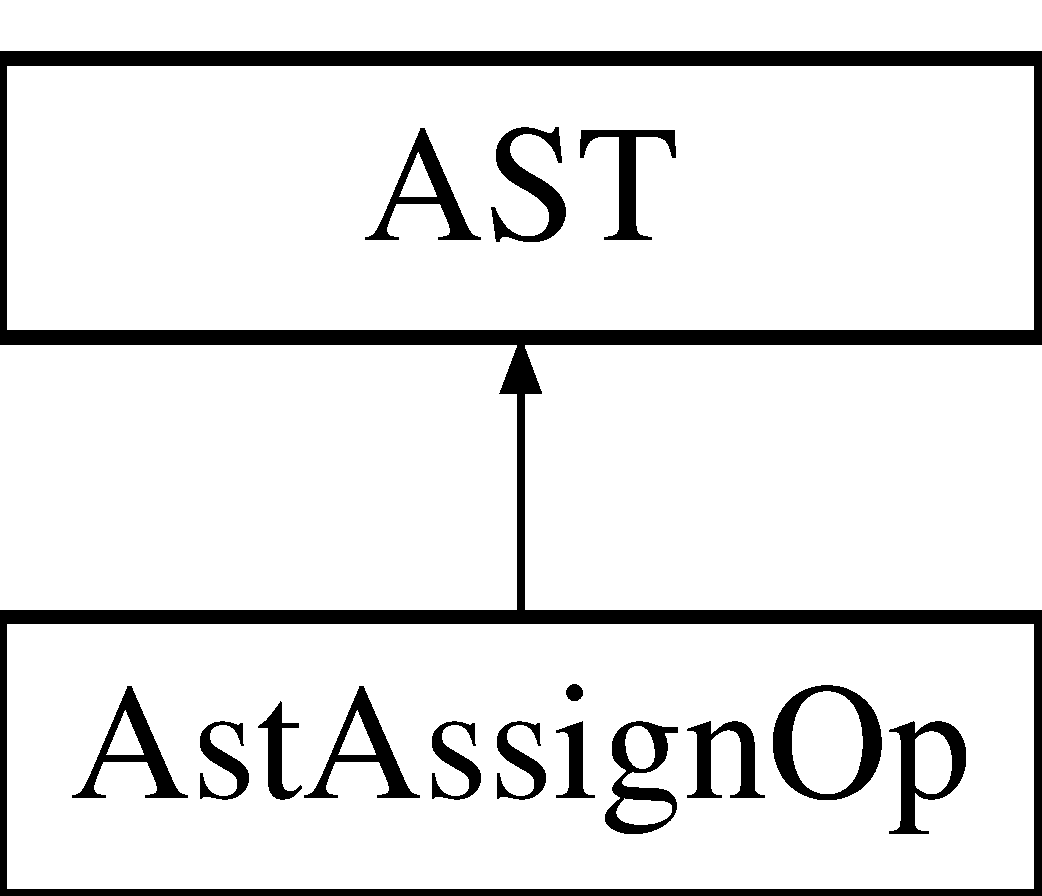
\includegraphics[height=2.000000cm]{classAstAssignOp}
\end{center}
\end{figure}
\subsection*{Public Types}
\begin{DoxyCompactItemize}
\item 
enum {\bfseries Operator} \{ \\*
{\bfseries E\-Q}, 
{\bfseries M\-U\-L\-\_\-\-A\-S\-S\-I\-G\-N}, 
{\bfseries D\-I\-V\-\_\-\-A\-S\-S\-I\-G\-N}, 
{\bfseries M\-O\-D\-\_\-\-A\-S\-S\-I\-G\-N}, 
\\*
{\bfseries A\-D\-D\-\_\-\-A\-S\-S\-I\-G\-N}, 
{\bfseries S\-U\-B\-\_\-\-A\-S\-S\-I\-G\-N}, 
{\bfseries L\-E\-F\-T\-\_\-\-A\-S\-S\-I\-G\-N}, 
{\bfseries R\-I\-G\-H\-T\-\_\-\-A\-S\-S\-I\-G\-N}, 
\\*
{\bfseries A\-N\-D\-\_\-\-A\-S\-S\-I\-G\-N}, 
{\bfseries X\-O\-R\-\_\-\-A\-S\-S\-I\-G\-N}, 
{\bfseries O\-R\-\_\-\-A\-S\-S\-I\-G\-N}, 
{\bfseries E\-Q}, 
\\*
{\bfseries M\-U\-L\-\_\-\-A\-S\-S\-I\-G\-N}, 
{\bfseries D\-I\-V\-\_\-\-A\-S\-S\-I\-G\-N}, 
{\bfseries M\-O\-D\-\_\-\-A\-S\-S\-I\-G\-N}, 
{\bfseries A\-D\-D\-\_\-\-A\-S\-S\-I\-G\-N}, 
\\*
{\bfseries S\-U\-B\-\_\-\-A\-S\-S\-I\-G\-N}, 
{\bfseries L\-E\-F\-T\-\_\-\-A\-S\-S\-I\-G\-N}, 
{\bfseries R\-I\-G\-H\-T\-\_\-\-A\-S\-S\-I\-G\-N}, 
{\bfseries A\-N\-D\-\_\-\-A\-S\-S\-I\-G\-N}, 
\\*
{\bfseries X\-O\-R\-\_\-\-A\-S\-S\-I\-G\-N}, 
{\bfseries O\-R\-\_\-\-A\-S\-S\-I\-G\-N}, 
{\bfseries E\-Q}, 
{\bfseries M\-U\-L\-\_\-\-A\-S\-S\-I\-G\-N}, 
\\*
{\bfseries D\-I\-V\-\_\-\-A\-S\-S\-I\-G\-N}, 
{\bfseries M\-O\-D\-\_\-\-A\-S\-S\-I\-G\-N}, 
{\bfseries A\-D\-D\-\_\-\-A\-S\-S\-I\-G\-N}, 
{\bfseries S\-U\-B\-\_\-\-A\-S\-S\-I\-G\-N}, 
\\*
{\bfseries L\-E\-F\-T\-\_\-\-A\-S\-S\-I\-G\-N}, 
{\bfseries R\-I\-G\-H\-T\-\_\-\-A\-S\-S\-I\-G\-N}, 
{\bfseries A\-N\-D\-\_\-\-A\-S\-S\-I\-G\-N}, 
{\bfseries X\-O\-R\-\_\-\-A\-S\-S\-I\-G\-N}, 
\\*
{\bfseries O\-R\-\_\-\-A\-S\-S\-I\-G\-N}, 
{\bfseries E\-Q}, 
{\bfseries M\-U\-L\-\_\-\-A\-S\-S\-I\-G\-N}, 
{\bfseries D\-I\-V\-\_\-\-A\-S\-S\-I\-G\-N}, 
\\*
{\bfseries M\-O\-D\-\_\-\-A\-S\-S\-I\-G\-N}, 
{\bfseries A\-D\-D\-\_\-\-A\-S\-S\-I\-G\-N}, 
{\bfseries S\-U\-B\-\_\-\-A\-S\-S\-I\-G\-N}, 
{\bfseries L\-E\-F\-T\-\_\-\-A\-S\-S\-I\-G\-N}, 
\\*
{\bfseries R\-I\-G\-H\-T\-\_\-\-A\-S\-S\-I\-G\-N}, 
{\bfseries A\-N\-D\-\_\-\-A\-S\-S\-I\-G\-N}, 
{\bfseries X\-O\-R\-\_\-\-A\-S\-S\-I\-G\-N}, 
{\bfseries O\-R\-\_\-\-A\-S\-S\-I\-G\-N}
 \}
\item 
enum {\bfseries Operator} \{ \\*
{\bfseries E\-Q}, 
{\bfseries M\-U\-L\-\_\-\-A\-S\-S\-I\-G\-N}, 
{\bfseries D\-I\-V\-\_\-\-A\-S\-S\-I\-G\-N}, 
{\bfseries M\-O\-D\-\_\-\-A\-S\-S\-I\-G\-N}, 
\\*
{\bfseries A\-D\-D\-\_\-\-A\-S\-S\-I\-G\-N}, 
{\bfseries S\-U\-B\-\_\-\-A\-S\-S\-I\-G\-N}, 
{\bfseries L\-E\-F\-T\-\_\-\-A\-S\-S\-I\-G\-N}, 
{\bfseries R\-I\-G\-H\-T\-\_\-\-A\-S\-S\-I\-G\-N}, 
\\*
{\bfseries A\-N\-D\-\_\-\-A\-S\-S\-I\-G\-N}, 
{\bfseries X\-O\-R\-\_\-\-A\-S\-S\-I\-G\-N}, 
{\bfseries O\-R\-\_\-\-A\-S\-S\-I\-G\-N}, 
{\bfseries E\-Q}, 
\\*
{\bfseries M\-U\-L\-\_\-\-A\-S\-S\-I\-G\-N}, 
{\bfseries D\-I\-V\-\_\-\-A\-S\-S\-I\-G\-N}, 
{\bfseries M\-O\-D\-\_\-\-A\-S\-S\-I\-G\-N}, 
{\bfseries A\-D\-D\-\_\-\-A\-S\-S\-I\-G\-N}, 
\\*
{\bfseries S\-U\-B\-\_\-\-A\-S\-S\-I\-G\-N}, 
{\bfseries L\-E\-F\-T\-\_\-\-A\-S\-S\-I\-G\-N}, 
{\bfseries R\-I\-G\-H\-T\-\_\-\-A\-S\-S\-I\-G\-N}, 
{\bfseries A\-N\-D\-\_\-\-A\-S\-S\-I\-G\-N}, 
\\*
{\bfseries X\-O\-R\-\_\-\-A\-S\-S\-I\-G\-N}, 
{\bfseries O\-R\-\_\-\-A\-S\-S\-I\-G\-N}, 
{\bfseries E\-Q}, 
{\bfseries M\-U\-L\-\_\-\-A\-S\-S\-I\-G\-N}, 
\\*
{\bfseries D\-I\-V\-\_\-\-A\-S\-S\-I\-G\-N}, 
{\bfseries M\-O\-D\-\_\-\-A\-S\-S\-I\-G\-N}, 
{\bfseries A\-D\-D\-\_\-\-A\-S\-S\-I\-G\-N}, 
{\bfseries S\-U\-B\-\_\-\-A\-S\-S\-I\-G\-N}, 
\\*
{\bfseries L\-E\-F\-T\-\_\-\-A\-S\-S\-I\-G\-N}, 
{\bfseries R\-I\-G\-H\-T\-\_\-\-A\-S\-S\-I\-G\-N}, 
{\bfseries A\-N\-D\-\_\-\-A\-S\-S\-I\-G\-N}, 
{\bfseries X\-O\-R\-\_\-\-A\-S\-S\-I\-G\-N}, 
\\*
{\bfseries O\-R\-\_\-\-A\-S\-S\-I\-G\-N}, 
{\bfseries E\-Q}, 
{\bfseries M\-U\-L\-\_\-\-A\-S\-S\-I\-G\-N}, 
{\bfseries D\-I\-V\-\_\-\-A\-S\-S\-I\-G\-N}, 
\\*
{\bfseries M\-O\-D\-\_\-\-A\-S\-S\-I\-G\-N}, 
{\bfseries A\-D\-D\-\_\-\-A\-S\-S\-I\-G\-N}, 
{\bfseries S\-U\-B\-\_\-\-A\-S\-S\-I\-G\-N}, 
{\bfseries L\-E\-F\-T\-\_\-\-A\-S\-S\-I\-G\-N}, 
\\*
{\bfseries R\-I\-G\-H\-T\-\_\-\-A\-S\-S\-I\-G\-N}, 
{\bfseries A\-N\-D\-\_\-\-A\-S\-S\-I\-G\-N}, 
{\bfseries X\-O\-R\-\_\-\-A\-S\-S\-I\-G\-N}, 
{\bfseries O\-R\-\_\-\-A\-S\-S\-I\-G\-N}
 \}
\item 
enum {\bfseries Operator} \{ \\*
{\bfseries E\-Q}, 
{\bfseries M\-U\-L\-\_\-\-A\-S\-S\-I\-G\-N}, 
{\bfseries D\-I\-V\-\_\-\-A\-S\-S\-I\-G\-N}, 
{\bfseries M\-O\-D\-\_\-\-A\-S\-S\-I\-G\-N}, 
\\*
{\bfseries A\-D\-D\-\_\-\-A\-S\-S\-I\-G\-N}, 
{\bfseries S\-U\-B\-\_\-\-A\-S\-S\-I\-G\-N}, 
{\bfseries L\-E\-F\-T\-\_\-\-A\-S\-S\-I\-G\-N}, 
{\bfseries R\-I\-G\-H\-T\-\_\-\-A\-S\-S\-I\-G\-N}, 
\\*
{\bfseries A\-N\-D\-\_\-\-A\-S\-S\-I\-G\-N}, 
{\bfseries X\-O\-R\-\_\-\-A\-S\-S\-I\-G\-N}, 
{\bfseries O\-R\-\_\-\-A\-S\-S\-I\-G\-N}, 
{\bfseries E\-Q}, 
\\*
{\bfseries M\-U\-L\-\_\-\-A\-S\-S\-I\-G\-N}, 
{\bfseries D\-I\-V\-\_\-\-A\-S\-S\-I\-G\-N}, 
{\bfseries M\-O\-D\-\_\-\-A\-S\-S\-I\-G\-N}, 
{\bfseries A\-D\-D\-\_\-\-A\-S\-S\-I\-G\-N}, 
\\*
{\bfseries S\-U\-B\-\_\-\-A\-S\-S\-I\-G\-N}, 
{\bfseries L\-E\-F\-T\-\_\-\-A\-S\-S\-I\-G\-N}, 
{\bfseries R\-I\-G\-H\-T\-\_\-\-A\-S\-S\-I\-G\-N}, 
{\bfseries A\-N\-D\-\_\-\-A\-S\-S\-I\-G\-N}, 
\\*
{\bfseries X\-O\-R\-\_\-\-A\-S\-S\-I\-G\-N}, 
{\bfseries O\-R\-\_\-\-A\-S\-S\-I\-G\-N}, 
{\bfseries E\-Q}, 
{\bfseries M\-U\-L\-\_\-\-A\-S\-S\-I\-G\-N}, 
\\*
{\bfseries D\-I\-V\-\_\-\-A\-S\-S\-I\-G\-N}, 
{\bfseries M\-O\-D\-\_\-\-A\-S\-S\-I\-G\-N}, 
{\bfseries A\-D\-D\-\_\-\-A\-S\-S\-I\-G\-N}, 
{\bfseries S\-U\-B\-\_\-\-A\-S\-S\-I\-G\-N}, 
\\*
{\bfseries L\-E\-F\-T\-\_\-\-A\-S\-S\-I\-G\-N}, 
{\bfseries R\-I\-G\-H\-T\-\_\-\-A\-S\-S\-I\-G\-N}, 
{\bfseries A\-N\-D\-\_\-\-A\-S\-S\-I\-G\-N}, 
{\bfseries X\-O\-R\-\_\-\-A\-S\-S\-I\-G\-N}, 
\\*
{\bfseries O\-R\-\_\-\-A\-S\-S\-I\-G\-N}, 
{\bfseries E\-Q}, 
{\bfseries M\-U\-L\-\_\-\-A\-S\-S\-I\-G\-N}, 
{\bfseries D\-I\-V\-\_\-\-A\-S\-S\-I\-G\-N}, 
\\*
{\bfseries M\-O\-D\-\_\-\-A\-S\-S\-I\-G\-N}, 
{\bfseries A\-D\-D\-\_\-\-A\-S\-S\-I\-G\-N}, 
{\bfseries S\-U\-B\-\_\-\-A\-S\-S\-I\-G\-N}, 
{\bfseries L\-E\-F\-T\-\_\-\-A\-S\-S\-I\-G\-N}, 
\\*
{\bfseries R\-I\-G\-H\-T\-\_\-\-A\-S\-S\-I\-G\-N}, 
{\bfseries A\-N\-D\-\_\-\-A\-S\-S\-I\-G\-N}, 
{\bfseries X\-O\-R\-\_\-\-A\-S\-S\-I\-G\-N}, 
{\bfseries O\-R\-\_\-\-A\-S\-S\-I\-G\-N}
 \}
\item 
enum {\bfseries Operator} \{ \\*
{\bfseries E\-Q}, 
{\bfseries M\-U\-L\-\_\-\-A\-S\-S\-I\-G\-N}, 
{\bfseries D\-I\-V\-\_\-\-A\-S\-S\-I\-G\-N}, 
{\bfseries M\-O\-D\-\_\-\-A\-S\-S\-I\-G\-N}, 
\\*
{\bfseries A\-D\-D\-\_\-\-A\-S\-S\-I\-G\-N}, 
{\bfseries S\-U\-B\-\_\-\-A\-S\-S\-I\-G\-N}, 
{\bfseries L\-E\-F\-T\-\_\-\-A\-S\-S\-I\-G\-N}, 
{\bfseries R\-I\-G\-H\-T\-\_\-\-A\-S\-S\-I\-G\-N}, 
\\*
{\bfseries A\-N\-D\-\_\-\-A\-S\-S\-I\-G\-N}, 
{\bfseries X\-O\-R\-\_\-\-A\-S\-S\-I\-G\-N}, 
{\bfseries O\-R\-\_\-\-A\-S\-S\-I\-G\-N}, 
{\bfseries E\-Q}, 
\\*
{\bfseries M\-U\-L\-\_\-\-A\-S\-S\-I\-G\-N}, 
{\bfseries D\-I\-V\-\_\-\-A\-S\-S\-I\-G\-N}, 
{\bfseries M\-O\-D\-\_\-\-A\-S\-S\-I\-G\-N}, 
{\bfseries A\-D\-D\-\_\-\-A\-S\-S\-I\-G\-N}, 
\\*
{\bfseries S\-U\-B\-\_\-\-A\-S\-S\-I\-G\-N}, 
{\bfseries L\-E\-F\-T\-\_\-\-A\-S\-S\-I\-G\-N}, 
{\bfseries R\-I\-G\-H\-T\-\_\-\-A\-S\-S\-I\-G\-N}, 
{\bfseries A\-N\-D\-\_\-\-A\-S\-S\-I\-G\-N}, 
\\*
{\bfseries X\-O\-R\-\_\-\-A\-S\-S\-I\-G\-N}, 
{\bfseries O\-R\-\_\-\-A\-S\-S\-I\-G\-N}, 
{\bfseries E\-Q}, 
{\bfseries M\-U\-L\-\_\-\-A\-S\-S\-I\-G\-N}, 
\\*
{\bfseries D\-I\-V\-\_\-\-A\-S\-S\-I\-G\-N}, 
{\bfseries M\-O\-D\-\_\-\-A\-S\-S\-I\-G\-N}, 
{\bfseries A\-D\-D\-\_\-\-A\-S\-S\-I\-G\-N}, 
{\bfseries S\-U\-B\-\_\-\-A\-S\-S\-I\-G\-N}, 
\\*
{\bfseries L\-E\-F\-T\-\_\-\-A\-S\-S\-I\-G\-N}, 
{\bfseries R\-I\-G\-H\-T\-\_\-\-A\-S\-S\-I\-G\-N}, 
{\bfseries A\-N\-D\-\_\-\-A\-S\-S\-I\-G\-N}, 
{\bfseries X\-O\-R\-\_\-\-A\-S\-S\-I\-G\-N}, 
\\*
{\bfseries O\-R\-\_\-\-A\-S\-S\-I\-G\-N}, 
{\bfseries E\-Q}, 
{\bfseries M\-U\-L\-\_\-\-A\-S\-S\-I\-G\-N}, 
{\bfseries D\-I\-V\-\_\-\-A\-S\-S\-I\-G\-N}, 
\\*
{\bfseries M\-O\-D\-\_\-\-A\-S\-S\-I\-G\-N}, 
{\bfseries A\-D\-D\-\_\-\-A\-S\-S\-I\-G\-N}, 
{\bfseries S\-U\-B\-\_\-\-A\-S\-S\-I\-G\-N}, 
{\bfseries L\-E\-F\-T\-\_\-\-A\-S\-S\-I\-G\-N}, 
\\*
{\bfseries R\-I\-G\-H\-T\-\_\-\-A\-S\-S\-I\-G\-N}, 
{\bfseries A\-N\-D\-\_\-\-A\-S\-S\-I\-G\-N}, 
{\bfseries X\-O\-R\-\_\-\-A\-S\-S\-I\-G\-N}, 
{\bfseries O\-R\-\_\-\-A\-S\-S\-I\-G\-N}
 \}
\end{DoxyCompactItemize}
\subsection*{Public Member Functions}
\begin{DoxyCompactItemize}
\item 
\hypertarget{classAstAssignOp_a456b3f679bb212a0520ca400536aa814}{{\bfseries Ast\-Assign\-Op} (Operator o)}\label{classAstAssignOp_a456b3f679bb212a0520ca400536aa814}

\item 
void \hyperlink{classAstAssignOp_a97614556953225b2fedc821732d9fa27}{Visit} ()
\begin{DoxyCompactList}\small\item\em This function is responsible for tree traversals. \end{DoxyCompactList}\item 
\hypertarget{classAstAssignOp_a456b3f679bb212a0520ca400536aa814}{{\bfseries Ast\-Assign\-Op} (Operator o)}\label{classAstAssignOp_a456b3f679bb212a0520ca400536aa814}

\item 
void \hyperlink{classAstAssignOp_a97614556953225b2fedc821732d9fa27}{Visit} ()
\begin{DoxyCompactList}\small\item\em This function is responsible for tree traversals. \end{DoxyCompactList}\item 
\hypertarget{classAstAssignOp_a456b3f679bb212a0520ca400536aa814}{{\bfseries Ast\-Assign\-Op} (Operator o)}\label{classAstAssignOp_a456b3f679bb212a0520ca400536aa814}

\item 
void \hyperlink{classAstAssignOp_a97614556953225b2fedc821732d9fa27}{Visit} ()
\begin{DoxyCompactList}\small\item\em This function is responsible for tree traversals. \end{DoxyCompactList}\item 
\hypertarget{classAstAssignOp_a456b3f679bb212a0520ca400536aa814}{{\bfseries Ast\-Assign\-Op} (Operator o)}\label{classAstAssignOp_a456b3f679bb212a0520ca400536aa814}

\item 
void \hyperlink{classAstAssignOp_a97614556953225b2fedc821732d9fa27}{Visit} ()
\begin{DoxyCompactList}\small\item\em This function is responsible for tree traversals. \end{DoxyCompactList}\item 
void \hyperlink{classAST_a71d680856e95ff89f55d5311a552eba6}{set\-Label} (string l)
\begin{DoxyCompactList}\small\item\em Sets the label for the node. \end{DoxyCompactList}\item 
void \hyperlink{classAST_a71d680856e95ff89f55d5311a552eba6}{set\-Label} (string l)
\begin{DoxyCompactList}\small\item\em Sets the label for the node. \end{DoxyCompactList}\item 
void \hyperlink{classAST_a71d680856e95ff89f55d5311a552eba6}{set\-Label} (string l)
\begin{DoxyCompactList}\small\item\em Sets the label for the node. \end{DoxyCompactList}\item 
void \hyperlink{classAST_a71d680856e95ff89f55d5311a552eba6}{set\-Label} (string l)
\begin{DoxyCompactList}\small\item\em Sets the label for the node. \end{DoxyCompactList}\item 
int \hyperlink{classAST_ab7a5b1d9f1c2de0d98deb356f724a42c}{get\-U\-I\-D} ()
\begin{DoxyCompactList}\small\item\em Gets the node's unique I\-D. \end{DoxyCompactList}\item 
int \hyperlink{classAST_ab7a5b1d9f1c2de0d98deb356f724a42c}{get\-U\-I\-D} ()
\begin{DoxyCompactList}\small\item\em Gets the node's unique I\-D. \end{DoxyCompactList}\item 
int \hyperlink{classAST_ab7a5b1d9f1c2de0d98deb356f724a42c}{get\-U\-I\-D} ()
\begin{DoxyCompactList}\small\item\em Gets the node's unique I\-D. \end{DoxyCompactList}\item 
int \hyperlink{classAST_ab7a5b1d9f1c2de0d98deb356f724a42c}{get\-U\-I\-D} ()
\begin{DoxyCompactList}\small\item\em Gets the node's unique I\-D. \end{DoxyCompactList}\item 
string \hyperlink{classAST_aee029be902fffc927d16ccb03eb922ad}{get\-Label} ()
\begin{DoxyCompactList}\small\item\em Gets the node's label. \end{DoxyCompactList}\item 
string \hyperlink{classAST_aee029be902fffc927d16ccb03eb922ad}{get\-Label} ()
\begin{DoxyCompactList}\small\item\em Gets the node's label. \end{DoxyCompactList}\item 
string \hyperlink{classAST_aee029be902fffc927d16ccb03eb922ad}{get\-Label} ()
\begin{DoxyCompactList}\small\item\em Gets the node's label. \end{DoxyCompactList}\item 
string \hyperlink{classAST_aee029be902fffc927d16ccb03eb922ad}{get\-Label} ()
\begin{DoxyCompactList}\small\item\em Gets the node's label. \end{DoxyCompactList}\end{DoxyCompactItemize}
\subsection*{Public Attributes}
\begin{DoxyCompactItemize}
\item 
\hypertarget{classAstAssignOp_a0c44cf716e74593ce0e303972dd79cf4}{Operator {\bfseries op}}\label{classAstAssignOp_a0c44cf716e74593ce0e303972dd79cf4}

\item 
\hypertarget{classAST_aaf215802de409f8096c063d01ffa6783}{bool \hyperlink{classAST_aaf215802de409f8096c063d01ffa6783}{needs\-Cast}}\label{classAST_aaf215802de409f8096c063d01ffa6783}

\begin{DoxyCompactList}\small\item\em This indicates if cast 3\-A\-C needs to be output, and is only relevant for expressions. \end{DoxyCompactList}\item 
\hypertarget{classAST_afa9e77ef650ec6664458fa6cb55be985}{bool \hyperlink{classAST_afa9e77ef650ec6664458fa6cb55be985}{is\-Conv}}\label{classAST_afa9e77ef650ec6664458fa6cb55be985}

\begin{DoxyCompactList}\small\item\em Indicates is a conversion is possible. \end{DoxyCompactList}\item 
\hypertarget{classAST_a61ef3317e023d45237e06615b387cd6b}{C\-O\-N\-V\-E\-R\-S\-I\-O\-N\-T\-Y\-P\-E \hyperlink{classAST_a61ef3317e023d45237e06615b387cd6b}{conv\-Type}}\label{classAST_a61ef3317e023d45237e06615b387cd6b}

\begin{DoxyCompactList}\small\item\em If needs\-Cast is true, then this indicates what the cast should be. \end{DoxyCompactList}\item 
\hypertarget{classAST_aea9b07b39d24183f38c0029cec0a878e}{int \hyperlink{classAST_aea9b07b39d24183f38c0029cec0a878e}{operand\-To\-Cast}}\label{classAST_aea9b07b39d24183f38c0029cec0a878e}

\begin{DoxyCompactList}\small\item\em This indicates if the first or second operand should be the one that is cast. \end{DoxyCompactList}\end{DoxyCompactItemize}
\subsection*{Static Public Attributes}
\begin{DoxyCompactItemize}
\item 
\hypertarget{classAST_a5fdfd5f7b104dd92889163bdadbc68d6}{static \hyperlink{classVisualizer}{Visualizer} \hyperlink{classAST_a5fdfd5f7b104dd92889163bdadbc68d6}{vis}}\label{classAST_a5fdfd5f7b104dd92889163bdadbc68d6}

\begin{DoxyCompactList}\small\item\em Static visualizer instance for generating the visualization of the \hyperlink{classAST}{A\-S\-T}. \end{DoxyCompactList}\item 
\hypertarget{classAST_a8a3ace322f50e030331065d644ee55ee}{static \hyperlink{classTAC__Generator}{T\-A\-C\-\_\-\-Generator} \hyperlink{classAST_a8a3ace322f50e030331065d644ee55ee}{tac\-Gen}}\label{classAST_a8a3ace322f50e030331065d644ee55ee}

\begin{DoxyCompactList}\small\item\em Three address code generator. \end{DoxyCompactList}\item 
\hypertarget{classAST_a1f69448c6dc368d005631a128460083d}{static string {\bfseries current\-Temp} =\char`\"{}\char`\"{}}\label{classAST_a1f69448c6dc368d005631a128460083d}

\item 
\hypertarget{classAST_a551aec090c932ab69365238b40a8a4eb}{static string \hyperlink{classAST_a551aec090c932ab69365238b40a8a4eb}{return\-Label} =\char`\"{}\char`\"{}}\label{classAST_a551aec090c932ab69365238b40a8a4eb}

\begin{DoxyCompactList}\small\item\em This is for storing the string id of any temporary result register that may be created during 3\-A\-C generation. \end{DoxyCompactList}\item 
\hypertarget{classAST_a73c0a266df52be71e6b527b6aa635173}{static list$<$ string $>$ {\bfseries temp\-Stack}}\label{classAST_a73c0a266df52be71e6b527b6aa635173}

\item 
\hypertarget{classAST_abf9e84b541ff04b7bb64e6e4371512d4}{static string {\bfseries last\-I\-D} =\char`\"{}\char`\"{}}\label{classAST_abf9e84b541ff04b7bb64e6e4371512d4}

\item 
\hypertarget{classAST_a163003bfe9c30510ec8039870346049f}{static \hyperlink{classSymTab}{Sym\-Tab} $\ast$ {\bfseries symbol\-Table} =N\-U\-L\-L}\label{classAST_a163003bfe9c30510ec8039870346049f}

\item 
\hypertarget{classAST_a5c3cc894d9c0453523dec9ed76f18a04}{static string {\bfseries current\-Function} =\char`\"{}\char`\"{}}\label{classAST_a5c3cc894d9c0453523dec9ed76f18a04}

\item 
\hypertarget{classAST_a66155513b59ff1a04c8ece8b20ec31f5}{static int {\bfseries current\-Constant\-Value} =0}\label{classAST_a66155513b59ff1a04c8ece8b20ec31f5}

\item 
\hypertarget{classAST_a3d031d7bab635ba1f015aade5943f40c}{static string {\bfseries current\-Id\-Name} =\char`\"{}\char`\"{}}\label{classAST_a3d031d7bab635ba1f015aade5943f40c}

\item 
\hypertarget{classAST_a16c4b6e54febc1a26b31a64a46972ef0}{static int {\bfseries current\-Index\-Val} = 0}\label{classAST_a16c4b6e54febc1a26b31a64a46972ef0}

\item 
\hypertarget{classAST_a6fc65ae9dd064a88941d4b88669b19db}{static string {\bfseries current\-I\-D} = \char`\"{}\char`\"{}}\label{classAST_a6fc65ae9dd064a88941d4b88669b19db}

\end{DoxyCompactItemize}
\subsection*{Protected Attributes}
\begin{DoxyCompactItemize}
\item 
\hypertarget{classAST_a847b778f1c3dd5a19de32de432ee6e15}{int \hyperlink{classAST_a847b778f1c3dd5a19de32de432ee6e15}{uid}}\label{classAST_a847b778f1c3dd5a19de32de432ee6e15}

\begin{DoxyCompactList}\small\item\em The unique id. \end{DoxyCompactList}\item 
\hypertarget{classAST_ab2e239ccc0688d2341724432ff5a1a31}{string \hyperlink{classAST_ab2e239ccc0688d2341724432ff5a1a31}{label}}\label{classAST_ab2e239ccc0688d2341724432ff5a1a31}

\begin{DoxyCompactList}\small\item\em The label to be printed in the visualization. \end{DoxyCompactList}\end{DoxyCompactItemize}


\subsection{Detailed Description}


Definition at line 726 of file Ast.\-h.



\subsection{Member Function Documentation}
\hypertarget{classAST_aee029be902fffc927d16ccb03eb922ad}{\index{Ast\-Assign\-Op@{Ast\-Assign\-Op}!get\-Label@{get\-Label}}
\index{get\-Label@{get\-Label}!AstAssignOp@{Ast\-Assign\-Op}}
\subsubsection[{get\-Label}]{\setlength{\rightskip}{0pt plus 5cm}string A\-S\-T\-::get\-Label (
\begin{DoxyParamCaption}
{}
\end{DoxyParamCaption}
)\hspace{0.3cm}{\ttfamily [inline]}, {\ttfamily [inherited]}}}\label{classAST_aee029be902fffc927d16ccb03eb922ad}


Gets the node's label. 

\begin{DoxyReturn}{Returns}
The label 
\end{DoxyReturn}


Definition at line 60 of file Ast.\-h.

\hypertarget{classAST_aee029be902fffc927d16ccb03eb922ad}{\index{Ast\-Assign\-Op@{Ast\-Assign\-Op}!get\-Label@{get\-Label}}
\index{get\-Label@{get\-Label}!AstAssignOp@{Ast\-Assign\-Op}}
\subsubsection[{get\-Label}]{\setlength{\rightskip}{0pt plus 5cm}string A\-S\-T\-::get\-Label (
\begin{DoxyParamCaption}
{}
\end{DoxyParamCaption}
)\hspace{0.3cm}{\ttfamily [inline]}, {\ttfamily [inherited]}}}\label{classAST_aee029be902fffc927d16ccb03eb922ad}


Gets the node's label. 

\begin{DoxyReturn}{Returns}
The label 
\end{DoxyReturn}


Definition at line 60 of file C\-Scanner.\-ll.

\hypertarget{classAST_aee029be902fffc927d16ccb03eb922ad}{\index{Ast\-Assign\-Op@{Ast\-Assign\-Op}!get\-Label@{get\-Label}}
\index{get\-Label@{get\-Label}!AstAssignOp@{Ast\-Assign\-Op}}
\subsubsection[{get\-Label}]{\setlength{\rightskip}{0pt plus 5cm}string A\-S\-T\-::get\-Label (
\begin{DoxyParamCaption}
{}
\end{DoxyParamCaption}
)\hspace{0.3cm}{\ttfamily [inline]}, {\ttfamily [inherited]}}}\label{classAST_aee029be902fffc927d16ccb03eb922ad}


Gets the node's label. 

\begin{DoxyReturn}{Returns}
The label 
\end{DoxyReturn}


Definition at line 60 of file C\-Parser.\-yy.

\hypertarget{classAST_aee029be902fffc927d16ccb03eb922ad}{\index{Ast\-Assign\-Op@{Ast\-Assign\-Op}!get\-Label@{get\-Label}}
\index{get\-Label@{get\-Label}!AstAssignOp@{Ast\-Assign\-Op}}
\subsubsection[{get\-Label}]{\setlength{\rightskip}{0pt plus 5cm}string A\-S\-T\-::get\-Label (
\begin{DoxyParamCaption}
{}
\end{DoxyParamCaption}
)\hspace{0.3cm}{\ttfamily [inline]}, {\ttfamily [inherited]}}}\label{classAST_aee029be902fffc927d16ccb03eb922ad}


Gets the node's label. 

\begin{DoxyReturn}{Returns}
The label 
\end{DoxyReturn}


Definition at line 60 of file C\-Parser.\-yy.

\hypertarget{classAST_ab7a5b1d9f1c2de0d98deb356f724a42c}{\index{Ast\-Assign\-Op@{Ast\-Assign\-Op}!get\-U\-I\-D@{get\-U\-I\-D}}
\index{get\-U\-I\-D@{get\-U\-I\-D}!AstAssignOp@{Ast\-Assign\-Op}}
\subsubsection[{get\-U\-I\-D}]{\setlength{\rightskip}{0pt plus 5cm}int A\-S\-T\-::get\-U\-I\-D (
\begin{DoxyParamCaption}
{}
\end{DoxyParamCaption}
)\hspace{0.3cm}{\ttfamily [inline]}, {\ttfamily [inherited]}}}\label{classAST_ab7a5b1d9f1c2de0d98deb356f724a42c}


Gets the node's unique I\-D. 

\begin{DoxyReturn}{Returns}
The unique id 
\end{DoxyReturn}


Definition at line 53 of file C\-Parser.\-yy.

\hypertarget{classAST_ab7a5b1d9f1c2de0d98deb356f724a42c}{\index{Ast\-Assign\-Op@{Ast\-Assign\-Op}!get\-U\-I\-D@{get\-U\-I\-D}}
\index{get\-U\-I\-D@{get\-U\-I\-D}!AstAssignOp@{Ast\-Assign\-Op}}
\subsubsection[{get\-U\-I\-D}]{\setlength{\rightskip}{0pt plus 5cm}int A\-S\-T\-::get\-U\-I\-D (
\begin{DoxyParamCaption}
{}
\end{DoxyParamCaption}
)\hspace{0.3cm}{\ttfamily [inline]}, {\ttfamily [inherited]}}}\label{classAST_ab7a5b1d9f1c2de0d98deb356f724a42c}


Gets the node's unique I\-D. 

\begin{DoxyReturn}{Returns}
The unique id 
\end{DoxyReturn}


Definition at line 53 of file C\-Parser.\-yy.

\hypertarget{classAST_ab7a5b1d9f1c2de0d98deb356f724a42c}{\index{Ast\-Assign\-Op@{Ast\-Assign\-Op}!get\-U\-I\-D@{get\-U\-I\-D}}
\index{get\-U\-I\-D@{get\-U\-I\-D}!AstAssignOp@{Ast\-Assign\-Op}}
\subsubsection[{get\-U\-I\-D}]{\setlength{\rightskip}{0pt plus 5cm}int A\-S\-T\-::get\-U\-I\-D (
\begin{DoxyParamCaption}
{}
\end{DoxyParamCaption}
)\hspace{0.3cm}{\ttfamily [inline]}, {\ttfamily [inherited]}}}\label{classAST_ab7a5b1d9f1c2de0d98deb356f724a42c}


Gets the node's unique I\-D. 

\begin{DoxyReturn}{Returns}
The unique id 
\end{DoxyReturn}


Definition at line 53 of file C\-Scanner.\-ll.

\hypertarget{classAST_ab7a5b1d9f1c2de0d98deb356f724a42c}{\index{Ast\-Assign\-Op@{Ast\-Assign\-Op}!get\-U\-I\-D@{get\-U\-I\-D}}
\index{get\-U\-I\-D@{get\-U\-I\-D}!AstAssignOp@{Ast\-Assign\-Op}}
\subsubsection[{get\-U\-I\-D}]{\setlength{\rightskip}{0pt plus 5cm}int A\-S\-T\-::get\-U\-I\-D (
\begin{DoxyParamCaption}
{}
\end{DoxyParamCaption}
)\hspace{0.3cm}{\ttfamily [inline]}, {\ttfamily [inherited]}}}\label{classAST_ab7a5b1d9f1c2de0d98deb356f724a42c}


Gets the node's unique I\-D. 

\begin{DoxyReturn}{Returns}
The unique id 
\end{DoxyReturn}


Definition at line 53 of file Ast.\-h.

\hypertarget{classAST_a71d680856e95ff89f55d5311a552eba6}{\index{Ast\-Assign\-Op@{Ast\-Assign\-Op}!set\-Label@{set\-Label}}
\index{set\-Label@{set\-Label}!AstAssignOp@{Ast\-Assign\-Op}}
\subsubsection[{set\-Label}]{\setlength{\rightskip}{0pt plus 5cm}void A\-S\-T\-::set\-Label (
\begin{DoxyParamCaption}
\item[{string}]{l}
\end{DoxyParamCaption}
)\hspace{0.3cm}{\ttfamily [inline]}, {\ttfamily [inherited]}}}\label{classAST_a71d680856e95ff89f55d5311a552eba6}


Sets the label for the node. 


\begin{DoxyParams}{Parameters}
{\em l} & The label string \\
\hline
\end{DoxyParams}


Definition at line 43 of file C\-Scanner.\-ll.

\hypertarget{classAST_a71d680856e95ff89f55d5311a552eba6}{\index{Ast\-Assign\-Op@{Ast\-Assign\-Op}!set\-Label@{set\-Label}}
\index{set\-Label@{set\-Label}!AstAssignOp@{Ast\-Assign\-Op}}
\subsubsection[{set\-Label}]{\setlength{\rightskip}{0pt plus 5cm}void A\-S\-T\-::set\-Label (
\begin{DoxyParamCaption}
\item[{string}]{l}
\end{DoxyParamCaption}
)\hspace{0.3cm}{\ttfamily [inline]}, {\ttfamily [inherited]}}}\label{classAST_a71d680856e95ff89f55d5311a552eba6}


Sets the label for the node. 


\begin{DoxyParams}{Parameters}
{\em l} & The label string \\
\hline
\end{DoxyParams}


Definition at line 43 of file C\-Parser.\-yy.

\hypertarget{classAST_a71d680856e95ff89f55d5311a552eba6}{\index{Ast\-Assign\-Op@{Ast\-Assign\-Op}!set\-Label@{set\-Label}}
\index{set\-Label@{set\-Label}!AstAssignOp@{Ast\-Assign\-Op}}
\subsubsection[{set\-Label}]{\setlength{\rightskip}{0pt plus 5cm}void A\-S\-T\-::set\-Label (
\begin{DoxyParamCaption}
\item[{string}]{l}
\end{DoxyParamCaption}
)\hspace{0.3cm}{\ttfamily [inline]}, {\ttfamily [inherited]}}}\label{classAST_a71d680856e95ff89f55d5311a552eba6}


Sets the label for the node. 


\begin{DoxyParams}{Parameters}
{\em l} & The label string \\
\hline
\end{DoxyParams}


Definition at line 43 of file Ast.\-h.

\hypertarget{classAST_a71d680856e95ff89f55d5311a552eba6}{\index{Ast\-Assign\-Op@{Ast\-Assign\-Op}!set\-Label@{set\-Label}}
\index{set\-Label@{set\-Label}!AstAssignOp@{Ast\-Assign\-Op}}
\subsubsection[{set\-Label}]{\setlength{\rightskip}{0pt plus 5cm}void A\-S\-T\-::set\-Label (
\begin{DoxyParamCaption}
\item[{string}]{l}
\end{DoxyParamCaption}
)\hspace{0.3cm}{\ttfamily [inline]}, {\ttfamily [inherited]}}}\label{classAST_a71d680856e95ff89f55d5311a552eba6}


Sets the label for the node. 


\begin{DoxyParams}{Parameters}
{\em l} & The label string \\
\hline
\end{DoxyParams}


Definition at line 43 of file C\-Parser.\-yy.

\hypertarget{classAstAssignOp_a97614556953225b2fedc821732d9fa27}{\index{Ast\-Assign\-Op@{Ast\-Assign\-Op}!Visit@{Visit}}
\index{Visit@{Visit}!AstAssignOp@{Ast\-Assign\-Op}}
\subsubsection[{Visit}]{\setlength{\rightskip}{0pt plus 5cm}void Ast\-Assign\-Op\-::\-Visit (
\begin{DoxyParamCaption}
{}
\end{DoxyParamCaption}
)\hspace{0.3cm}{\ttfamily [virtual]}}}\label{classAstAssignOp_a97614556953225b2fedc821732d9fa27}


This function is responsible for tree traversals. 

This function will call the Visit functions of each of it's children nodes, call the visualization code for itself, and output any 3\-A\-C that can be generated at the current node. 

Reimplemented from \hyperlink{classAST_a5828cc86f2c4f1a0aeab6d7069e8fd82}{A\-S\-T}.



Definition at line 1858 of file Ast.\-cpp.

\hypertarget{classAstAssignOp_a97614556953225b2fedc821732d9fa27}{\index{Ast\-Assign\-Op@{Ast\-Assign\-Op}!Visit@{Visit}}
\index{Visit@{Visit}!AstAssignOp@{Ast\-Assign\-Op}}
\subsubsection[{Visit}]{\setlength{\rightskip}{0pt plus 5cm}void Ast\-Assign\-Op\-::\-Visit (
\begin{DoxyParamCaption}
{}
\end{DoxyParamCaption}
)\hspace{0.3cm}{\ttfamily [virtual]}}}\label{classAstAssignOp_a97614556953225b2fedc821732d9fa27}


This function is responsible for tree traversals. 

This function will call the Visit functions of each of it's children nodes, call the visualization code for itself, and output any 3\-A\-C that can be generated at the current node. 

Reimplemented from \hyperlink{classAST_a5828cc86f2c4f1a0aeab6d7069e8fd82}{A\-S\-T}.

\hypertarget{classAstAssignOp_a97614556953225b2fedc821732d9fa27}{\index{Ast\-Assign\-Op@{Ast\-Assign\-Op}!Visit@{Visit}}
\index{Visit@{Visit}!AstAssignOp@{Ast\-Assign\-Op}}
\subsubsection[{Visit}]{\setlength{\rightskip}{0pt plus 5cm}void Ast\-Assign\-Op\-::\-Visit (
\begin{DoxyParamCaption}
{}
\end{DoxyParamCaption}
)\hspace{0.3cm}{\ttfamily [virtual]}}}\label{classAstAssignOp_a97614556953225b2fedc821732d9fa27}


This function is responsible for tree traversals. 

This function will call the Visit functions of each of it's children nodes, call the visualization code for itself, and output any 3\-A\-C that can be generated at the current node. 

Reimplemented from \hyperlink{classAST_a5828cc86f2c4f1a0aeab6d7069e8fd82}{A\-S\-T}.

\hypertarget{classAstAssignOp_a97614556953225b2fedc821732d9fa27}{\index{Ast\-Assign\-Op@{Ast\-Assign\-Op}!Visit@{Visit}}
\index{Visit@{Visit}!AstAssignOp@{Ast\-Assign\-Op}}
\subsubsection[{Visit}]{\setlength{\rightskip}{0pt plus 5cm}void Ast\-Assign\-Op\-::\-Visit (
\begin{DoxyParamCaption}
{}
\end{DoxyParamCaption}
)\hspace{0.3cm}{\ttfamily [virtual]}}}\label{classAstAssignOp_a97614556953225b2fedc821732d9fa27}


This function is responsible for tree traversals. 

This function will call the Visit functions of each of it's children nodes, call the visualization code for itself, and output any 3\-A\-C that can be generated at the current node. 

Reimplemented from \hyperlink{classAST_a5828cc86f2c4f1a0aeab6d7069e8fd82}{A\-S\-T}.



The documentation for this class was generated from the following files\-:\begin{DoxyCompactItemize}
\item 
Ast.\-h\item 
Ast.\-cpp\end{DoxyCompactItemize}

\hypertarget{classAstBreak}{\section{Ast\-Break Class Reference}
\label{classAstBreak}\index{Ast\-Break@{Ast\-Break}}
}
Inheritance diagram for Ast\-Break\-:\begin{figure}[H]
\begin{center}
\leavevmode
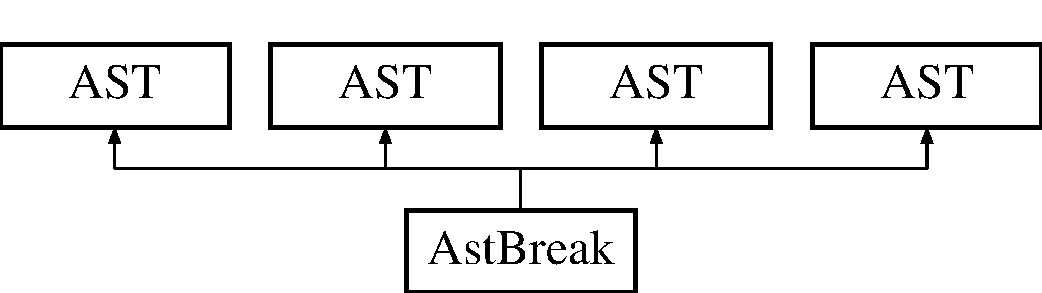
\includegraphics[height=2.000000cm]{classAstBreak}
\end{center}
\end{figure}
\subsection*{Public Member Functions}
\begin{DoxyCompactItemize}
\item 
void \hyperlink{classAstBreak_added06a2e2ceaec2839df436a6fbf911}{Visit} ()
\begin{DoxyCompactList}\small\item\em This function is responsible for tree traversals. \end{DoxyCompactList}\item 
void \hyperlink{classAstBreak_added06a2e2ceaec2839df436a6fbf911}{Visit} ()
\begin{DoxyCompactList}\small\item\em This function is responsible for tree traversals. \end{DoxyCompactList}\item 
void \hyperlink{classAstBreak_added06a2e2ceaec2839df436a6fbf911}{Visit} ()
\begin{DoxyCompactList}\small\item\em This function is responsible for tree traversals. \end{DoxyCompactList}\item 
void \hyperlink{classAstBreak_added06a2e2ceaec2839df436a6fbf911}{Visit} ()
\begin{DoxyCompactList}\small\item\em This function is responsible for tree traversals. \end{DoxyCompactList}\item 
void \hyperlink{classAST_a71d680856e95ff89f55d5311a552eba6}{set\-Label} (string l)
\begin{DoxyCompactList}\small\item\em Sets the label for the node. \end{DoxyCompactList}\item 
void \hyperlink{classAST_a71d680856e95ff89f55d5311a552eba6}{set\-Label} (string l)
\begin{DoxyCompactList}\small\item\em Sets the label for the node. \end{DoxyCompactList}\item 
void \hyperlink{classAST_a71d680856e95ff89f55d5311a552eba6}{set\-Label} (string l)
\begin{DoxyCompactList}\small\item\em Sets the label for the node. \end{DoxyCompactList}\item 
void \hyperlink{classAST_a71d680856e95ff89f55d5311a552eba6}{set\-Label} (string l)
\begin{DoxyCompactList}\small\item\em Sets the label for the node. \end{DoxyCompactList}\item 
int \hyperlink{classAST_ab7a5b1d9f1c2de0d98deb356f724a42c}{get\-U\-I\-D} ()
\begin{DoxyCompactList}\small\item\em Gets the node's unique I\-D. \end{DoxyCompactList}\item 
int \hyperlink{classAST_ab7a5b1d9f1c2de0d98deb356f724a42c}{get\-U\-I\-D} ()
\begin{DoxyCompactList}\small\item\em Gets the node's unique I\-D. \end{DoxyCompactList}\item 
int \hyperlink{classAST_ab7a5b1d9f1c2de0d98deb356f724a42c}{get\-U\-I\-D} ()
\begin{DoxyCompactList}\small\item\em Gets the node's unique I\-D. \end{DoxyCompactList}\item 
int \hyperlink{classAST_ab7a5b1d9f1c2de0d98deb356f724a42c}{get\-U\-I\-D} ()
\begin{DoxyCompactList}\small\item\em Gets the node's unique I\-D. \end{DoxyCompactList}\item 
string \hyperlink{classAST_aee029be902fffc927d16ccb03eb922ad}{get\-Label} ()
\begin{DoxyCompactList}\small\item\em Gets the node's label. \end{DoxyCompactList}\item 
string \hyperlink{classAST_aee029be902fffc927d16ccb03eb922ad}{get\-Label} ()
\begin{DoxyCompactList}\small\item\em Gets the node's label. \end{DoxyCompactList}\item 
string \hyperlink{classAST_aee029be902fffc927d16ccb03eb922ad}{get\-Label} ()
\begin{DoxyCompactList}\small\item\em Gets the node's label. \end{DoxyCompactList}\item 
string \hyperlink{classAST_aee029be902fffc927d16ccb03eb922ad}{get\-Label} ()
\begin{DoxyCompactList}\small\item\em Gets the node's label. \end{DoxyCompactList}\end{DoxyCompactItemize}
\subsection*{Public Attributes}
\begin{DoxyCompactItemize}
\item 
\hypertarget{classAST_aaf215802de409f8096c063d01ffa6783}{bool \hyperlink{classAST_aaf215802de409f8096c063d01ffa6783}{needs\-Cast}}\label{classAST_aaf215802de409f8096c063d01ffa6783}

\begin{DoxyCompactList}\small\item\em This indicates if cast 3\-A\-C needs to be output, and is only relevant for expressions. \end{DoxyCompactList}\item 
\hypertarget{classAST_afa9e77ef650ec6664458fa6cb55be985}{bool \hyperlink{classAST_afa9e77ef650ec6664458fa6cb55be985}{is\-Conv}}\label{classAST_afa9e77ef650ec6664458fa6cb55be985}

\begin{DoxyCompactList}\small\item\em Indicates is a conversion is possible. \end{DoxyCompactList}\item 
\hypertarget{classAST_a61ef3317e023d45237e06615b387cd6b}{C\-O\-N\-V\-E\-R\-S\-I\-O\-N\-T\-Y\-P\-E \hyperlink{classAST_a61ef3317e023d45237e06615b387cd6b}{conv\-Type}}\label{classAST_a61ef3317e023d45237e06615b387cd6b}

\begin{DoxyCompactList}\small\item\em If needs\-Cast is true, then this indicates what the cast should be. \end{DoxyCompactList}\item 
\hypertarget{classAST_aea9b07b39d24183f38c0029cec0a878e}{int \hyperlink{classAST_aea9b07b39d24183f38c0029cec0a878e}{operand\-To\-Cast}}\label{classAST_aea9b07b39d24183f38c0029cec0a878e}

\begin{DoxyCompactList}\small\item\em This indicates if the first or second operand should be the one that is cast. \end{DoxyCompactList}\end{DoxyCompactItemize}
\subsection*{Static Public Attributes}
\begin{DoxyCompactItemize}
\item 
\hypertarget{classAST_a5fdfd5f7b104dd92889163bdadbc68d6}{static \hyperlink{classVisualizer}{Visualizer} \hyperlink{classAST_a5fdfd5f7b104dd92889163bdadbc68d6}{vis}}\label{classAST_a5fdfd5f7b104dd92889163bdadbc68d6}

\begin{DoxyCompactList}\small\item\em Static visualizer instance for generating the visualization of the \hyperlink{classAST}{A\-S\-T}. \end{DoxyCompactList}\item 
\hypertarget{classAST_a8a3ace322f50e030331065d644ee55ee}{static \hyperlink{classTAC__Generator}{T\-A\-C\-\_\-\-Generator} \hyperlink{classAST_a8a3ace322f50e030331065d644ee55ee}{tac\-Gen}}\label{classAST_a8a3ace322f50e030331065d644ee55ee}

\begin{DoxyCompactList}\small\item\em Three address code generator. \end{DoxyCompactList}\item 
\hypertarget{classAST_a1f69448c6dc368d005631a128460083d}{static string {\bfseries current\-Temp} =\char`\"{}\char`\"{}}\label{classAST_a1f69448c6dc368d005631a128460083d}

\item 
\hypertarget{classAST_a551aec090c932ab69365238b40a8a4eb}{static string \hyperlink{classAST_a551aec090c932ab69365238b40a8a4eb}{return\-Label} =\char`\"{}\char`\"{}}\label{classAST_a551aec090c932ab69365238b40a8a4eb}

\begin{DoxyCompactList}\small\item\em This is for storing the string id of any temporary result register that may be created during 3\-A\-C generation. \end{DoxyCompactList}\item 
\hypertarget{classAST_a73c0a266df52be71e6b527b6aa635173}{static list$<$ string $>$ {\bfseries temp\-Stack}}\label{classAST_a73c0a266df52be71e6b527b6aa635173}

\item 
\hypertarget{classAST_abf9e84b541ff04b7bb64e6e4371512d4}{static string {\bfseries last\-I\-D} =\char`\"{}\char`\"{}}\label{classAST_abf9e84b541ff04b7bb64e6e4371512d4}

\item 
\hypertarget{classAST_a163003bfe9c30510ec8039870346049f}{static \hyperlink{classSymTab}{Sym\-Tab} $\ast$ {\bfseries symbol\-Table} =N\-U\-L\-L}\label{classAST_a163003bfe9c30510ec8039870346049f}

\item 
\hypertarget{classAST_a5c3cc894d9c0453523dec9ed76f18a04}{static string {\bfseries current\-Function} =\char`\"{}\char`\"{}}\label{classAST_a5c3cc894d9c0453523dec9ed76f18a04}

\end{DoxyCompactItemize}
\subsection*{Protected Attributes}
\begin{DoxyCompactItemize}
\item 
\hypertarget{classAST_a847b778f1c3dd5a19de32de432ee6e15}{int \hyperlink{classAST_a847b778f1c3dd5a19de32de432ee6e15}{uid}}\label{classAST_a847b778f1c3dd5a19de32de432ee6e15}

\begin{DoxyCompactList}\small\item\em The unique id. \end{DoxyCompactList}\item 
\hypertarget{classAST_ab2e239ccc0688d2341724432ff5a1a31}{string \hyperlink{classAST_ab2e239ccc0688d2341724432ff5a1a31}{label}}\label{classAST_ab2e239ccc0688d2341724432ff5a1a31}

\begin{DoxyCompactList}\small\item\em The label to be printed in the visualization. \end{DoxyCompactList}\end{DoxyCompactItemize}


\subsection{Detailed Description}


Definition at line 658 of file Ast.\-h.



\subsection{Member Function Documentation}
\hypertarget{classAST_aee029be902fffc927d16ccb03eb922ad}{\index{Ast\-Break@{Ast\-Break}!get\-Label@{get\-Label}}
\index{get\-Label@{get\-Label}!AstBreak@{Ast\-Break}}
\subsubsection[{get\-Label}]{\setlength{\rightskip}{0pt plus 5cm}string A\-S\-T\-::get\-Label (
\begin{DoxyParamCaption}
{}
\end{DoxyParamCaption}
)\hspace{0.3cm}{\ttfamily [inline]}, {\ttfamily [inherited]}}}\label{classAST_aee029be902fffc927d16ccb03eb922ad}


Gets the node's label. 

\begin{DoxyReturn}{Returns}
The label 
\end{DoxyReturn}


Definition at line 60 of file Ast.\-h.

\hypertarget{classAST_aee029be902fffc927d16ccb03eb922ad}{\index{Ast\-Break@{Ast\-Break}!get\-Label@{get\-Label}}
\index{get\-Label@{get\-Label}!AstBreak@{Ast\-Break}}
\subsubsection[{get\-Label}]{\setlength{\rightskip}{0pt plus 5cm}string A\-S\-T\-::get\-Label (
\begin{DoxyParamCaption}
{}
\end{DoxyParamCaption}
)\hspace{0.3cm}{\ttfamily [inline]}, {\ttfamily [inherited]}}}\label{classAST_aee029be902fffc927d16ccb03eb922ad}


Gets the node's label. 

\begin{DoxyReturn}{Returns}
The label 
\end{DoxyReturn}


Definition at line 60 of file C\-Scanner.\-ll.

\hypertarget{classAST_aee029be902fffc927d16ccb03eb922ad}{\index{Ast\-Break@{Ast\-Break}!get\-Label@{get\-Label}}
\index{get\-Label@{get\-Label}!AstBreak@{Ast\-Break}}
\subsubsection[{get\-Label}]{\setlength{\rightskip}{0pt plus 5cm}string A\-S\-T\-::get\-Label (
\begin{DoxyParamCaption}
{}
\end{DoxyParamCaption}
)\hspace{0.3cm}{\ttfamily [inline]}, {\ttfamily [inherited]}}}\label{classAST_aee029be902fffc927d16ccb03eb922ad}


Gets the node's label. 

\begin{DoxyReturn}{Returns}
The label 
\end{DoxyReturn}


Definition at line 60 of file C\-Parser.\-yy.

\hypertarget{classAST_aee029be902fffc927d16ccb03eb922ad}{\index{Ast\-Break@{Ast\-Break}!get\-Label@{get\-Label}}
\index{get\-Label@{get\-Label}!AstBreak@{Ast\-Break}}
\subsubsection[{get\-Label}]{\setlength{\rightskip}{0pt plus 5cm}string A\-S\-T\-::get\-Label (
\begin{DoxyParamCaption}
{}
\end{DoxyParamCaption}
)\hspace{0.3cm}{\ttfamily [inline]}, {\ttfamily [inherited]}}}\label{classAST_aee029be902fffc927d16ccb03eb922ad}


Gets the node's label. 

\begin{DoxyReturn}{Returns}
The label 
\end{DoxyReturn}


Definition at line 60 of file C\-Parser.\-yy.

\hypertarget{classAST_ab7a5b1d9f1c2de0d98deb356f724a42c}{\index{Ast\-Break@{Ast\-Break}!get\-U\-I\-D@{get\-U\-I\-D}}
\index{get\-U\-I\-D@{get\-U\-I\-D}!AstBreak@{Ast\-Break}}
\subsubsection[{get\-U\-I\-D}]{\setlength{\rightskip}{0pt plus 5cm}int A\-S\-T\-::get\-U\-I\-D (
\begin{DoxyParamCaption}
{}
\end{DoxyParamCaption}
)\hspace{0.3cm}{\ttfamily [inline]}, {\ttfamily [inherited]}}}\label{classAST_ab7a5b1d9f1c2de0d98deb356f724a42c}


Gets the node's unique I\-D. 

\begin{DoxyReturn}{Returns}
The unique id 
\end{DoxyReturn}


Definition at line 53 of file C\-Parser.\-yy.

\hypertarget{classAST_ab7a5b1d9f1c2de0d98deb356f724a42c}{\index{Ast\-Break@{Ast\-Break}!get\-U\-I\-D@{get\-U\-I\-D}}
\index{get\-U\-I\-D@{get\-U\-I\-D}!AstBreak@{Ast\-Break}}
\subsubsection[{get\-U\-I\-D}]{\setlength{\rightskip}{0pt plus 5cm}int A\-S\-T\-::get\-U\-I\-D (
\begin{DoxyParamCaption}
{}
\end{DoxyParamCaption}
)\hspace{0.3cm}{\ttfamily [inline]}, {\ttfamily [inherited]}}}\label{classAST_ab7a5b1d9f1c2de0d98deb356f724a42c}


Gets the node's unique I\-D. 

\begin{DoxyReturn}{Returns}
The unique id 
\end{DoxyReturn}


Definition at line 53 of file C\-Parser.\-yy.

\hypertarget{classAST_ab7a5b1d9f1c2de0d98deb356f724a42c}{\index{Ast\-Break@{Ast\-Break}!get\-U\-I\-D@{get\-U\-I\-D}}
\index{get\-U\-I\-D@{get\-U\-I\-D}!AstBreak@{Ast\-Break}}
\subsubsection[{get\-U\-I\-D}]{\setlength{\rightskip}{0pt plus 5cm}int A\-S\-T\-::get\-U\-I\-D (
\begin{DoxyParamCaption}
{}
\end{DoxyParamCaption}
)\hspace{0.3cm}{\ttfamily [inline]}, {\ttfamily [inherited]}}}\label{classAST_ab7a5b1d9f1c2de0d98deb356f724a42c}


Gets the node's unique I\-D. 

\begin{DoxyReturn}{Returns}
The unique id 
\end{DoxyReturn}


Definition at line 53 of file C\-Scanner.\-ll.

\hypertarget{classAST_ab7a5b1d9f1c2de0d98deb356f724a42c}{\index{Ast\-Break@{Ast\-Break}!get\-U\-I\-D@{get\-U\-I\-D}}
\index{get\-U\-I\-D@{get\-U\-I\-D}!AstBreak@{Ast\-Break}}
\subsubsection[{get\-U\-I\-D}]{\setlength{\rightskip}{0pt plus 5cm}int A\-S\-T\-::get\-U\-I\-D (
\begin{DoxyParamCaption}
{}
\end{DoxyParamCaption}
)\hspace{0.3cm}{\ttfamily [inline]}, {\ttfamily [inherited]}}}\label{classAST_ab7a5b1d9f1c2de0d98deb356f724a42c}


Gets the node's unique I\-D. 

\begin{DoxyReturn}{Returns}
The unique id 
\end{DoxyReturn}


Definition at line 53 of file Ast.\-h.

\hypertarget{classAST_a71d680856e95ff89f55d5311a552eba6}{\index{Ast\-Break@{Ast\-Break}!set\-Label@{set\-Label}}
\index{set\-Label@{set\-Label}!AstBreak@{Ast\-Break}}
\subsubsection[{set\-Label}]{\setlength{\rightskip}{0pt plus 5cm}void A\-S\-T\-::set\-Label (
\begin{DoxyParamCaption}
\item[{string}]{l}
\end{DoxyParamCaption}
)\hspace{0.3cm}{\ttfamily [inline]}, {\ttfamily [inherited]}}}\label{classAST_a71d680856e95ff89f55d5311a552eba6}


Sets the label for the node. 


\begin{DoxyParams}{Parameters}
{\em l} & The label string \\
\hline
\end{DoxyParams}


Definition at line 43 of file C\-Scanner.\-ll.

\hypertarget{classAST_a71d680856e95ff89f55d5311a552eba6}{\index{Ast\-Break@{Ast\-Break}!set\-Label@{set\-Label}}
\index{set\-Label@{set\-Label}!AstBreak@{Ast\-Break}}
\subsubsection[{set\-Label}]{\setlength{\rightskip}{0pt plus 5cm}void A\-S\-T\-::set\-Label (
\begin{DoxyParamCaption}
\item[{string}]{l}
\end{DoxyParamCaption}
)\hspace{0.3cm}{\ttfamily [inline]}, {\ttfamily [inherited]}}}\label{classAST_a71d680856e95ff89f55d5311a552eba6}


Sets the label for the node. 


\begin{DoxyParams}{Parameters}
{\em l} & The label string \\
\hline
\end{DoxyParams}


Definition at line 43 of file C\-Parser.\-yy.

\hypertarget{classAST_a71d680856e95ff89f55d5311a552eba6}{\index{Ast\-Break@{Ast\-Break}!set\-Label@{set\-Label}}
\index{set\-Label@{set\-Label}!AstBreak@{Ast\-Break}}
\subsubsection[{set\-Label}]{\setlength{\rightskip}{0pt plus 5cm}void A\-S\-T\-::set\-Label (
\begin{DoxyParamCaption}
\item[{string}]{l}
\end{DoxyParamCaption}
)\hspace{0.3cm}{\ttfamily [inline]}, {\ttfamily [inherited]}}}\label{classAST_a71d680856e95ff89f55d5311a552eba6}


Sets the label for the node. 


\begin{DoxyParams}{Parameters}
{\em l} & The label string \\
\hline
\end{DoxyParams}


Definition at line 43 of file Ast.\-h.

\hypertarget{classAST_a71d680856e95ff89f55d5311a552eba6}{\index{Ast\-Break@{Ast\-Break}!set\-Label@{set\-Label}}
\index{set\-Label@{set\-Label}!AstBreak@{Ast\-Break}}
\subsubsection[{set\-Label}]{\setlength{\rightskip}{0pt plus 5cm}void A\-S\-T\-::set\-Label (
\begin{DoxyParamCaption}
\item[{string}]{l}
\end{DoxyParamCaption}
)\hspace{0.3cm}{\ttfamily [inline]}, {\ttfamily [inherited]}}}\label{classAST_a71d680856e95ff89f55d5311a552eba6}


Sets the label for the node. 


\begin{DoxyParams}{Parameters}
{\em l} & The label string \\
\hline
\end{DoxyParams}


Definition at line 43 of file C\-Parser.\-yy.

\hypertarget{classAstBreak_added06a2e2ceaec2839df436a6fbf911}{\index{Ast\-Break@{Ast\-Break}!Visit@{Visit}}
\index{Visit@{Visit}!AstBreak@{Ast\-Break}}
\subsubsection[{Visit}]{\setlength{\rightskip}{0pt plus 5cm}void Ast\-Break\-::\-Visit (
\begin{DoxyParamCaption}
{}
\end{DoxyParamCaption}
)\hspace{0.3cm}{\ttfamily [virtual]}}}\label{classAstBreak_added06a2e2ceaec2839df436a6fbf911}


This function is responsible for tree traversals. 

This function will call the Visit functions of each of it's children nodes, call the visualization code for itself, and output any 3\-A\-C that can be generated at the current node. 

Reimplemented from \hyperlink{classAST_a5828cc86f2c4f1a0aeab6d7069e8fd82}{A\-S\-T}.



Definition at line 1924 of file Ast.\-cpp.

\hypertarget{classAstBreak_added06a2e2ceaec2839df436a6fbf911}{\index{Ast\-Break@{Ast\-Break}!Visit@{Visit}}
\index{Visit@{Visit}!AstBreak@{Ast\-Break}}
\subsubsection[{Visit}]{\setlength{\rightskip}{0pt plus 5cm}void Ast\-Break\-::\-Visit (
\begin{DoxyParamCaption}
{}
\end{DoxyParamCaption}
)\hspace{0.3cm}{\ttfamily [virtual]}}}\label{classAstBreak_added06a2e2ceaec2839df436a6fbf911}


This function is responsible for tree traversals. 

This function will call the Visit functions of each of it's children nodes, call the visualization code for itself, and output any 3\-A\-C that can be generated at the current node. 

Reimplemented from \hyperlink{classAST_a5828cc86f2c4f1a0aeab6d7069e8fd82}{A\-S\-T}.

\hypertarget{classAstBreak_added06a2e2ceaec2839df436a6fbf911}{\index{Ast\-Break@{Ast\-Break}!Visit@{Visit}}
\index{Visit@{Visit}!AstBreak@{Ast\-Break}}
\subsubsection[{Visit}]{\setlength{\rightskip}{0pt plus 5cm}void Ast\-Break\-::\-Visit (
\begin{DoxyParamCaption}
{}
\end{DoxyParamCaption}
)\hspace{0.3cm}{\ttfamily [virtual]}}}\label{classAstBreak_added06a2e2ceaec2839df436a6fbf911}


This function is responsible for tree traversals. 

This function will call the Visit functions of each of it's children nodes, call the visualization code for itself, and output any 3\-A\-C that can be generated at the current node. 

Reimplemented from \hyperlink{classAST_a5828cc86f2c4f1a0aeab6d7069e8fd82}{A\-S\-T}.

\hypertarget{classAstBreak_added06a2e2ceaec2839df436a6fbf911}{\index{Ast\-Break@{Ast\-Break}!Visit@{Visit}}
\index{Visit@{Visit}!AstBreak@{Ast\-Break}}
\subsubsection[{Visit}]{\setlength{\rightskip}{0pt plus 5cm}void Ast\-Break\-::\-Visit (
\begin{DoxyParamCaption}
{}
\end{DoxyParamCaption}
)\hspace{0.3cm}{\ttfamily [virtual]}}}\label{classAstBreak_added06a2e2ceaec2839df436a6fbf911}


This function is responsible for tree traversals. 

This function will call the Visit functions of each of it's children nodes, call the visualization code for itself, and output any 3\-A\-C that can be generated at the current node. 

Reimplemented from \hyperlink{classAST_a5828cc86f2c4f1a0aeab6d7069e8fd82}{A\-S\-T}.



The documentation for this class was generated from the following files\-:\begin{DoxyCompactItemize}
\item 
Ast.\-h\item 
Ast.\-cpp\end{DoxyCompactItemize}

\hypertarget{classAstCastExpr}{\section{Ast\-Cast\-Expr Class Reference}
\label{classAstCastExpr}\index{Ast\-Cast\-Expr@{Ast\-Cast\-Expr}}
}
Inheritance diagram for Ast\-Cast\-Expr\-:\begin{figure}[H]
\begin{center}
\leavevmode
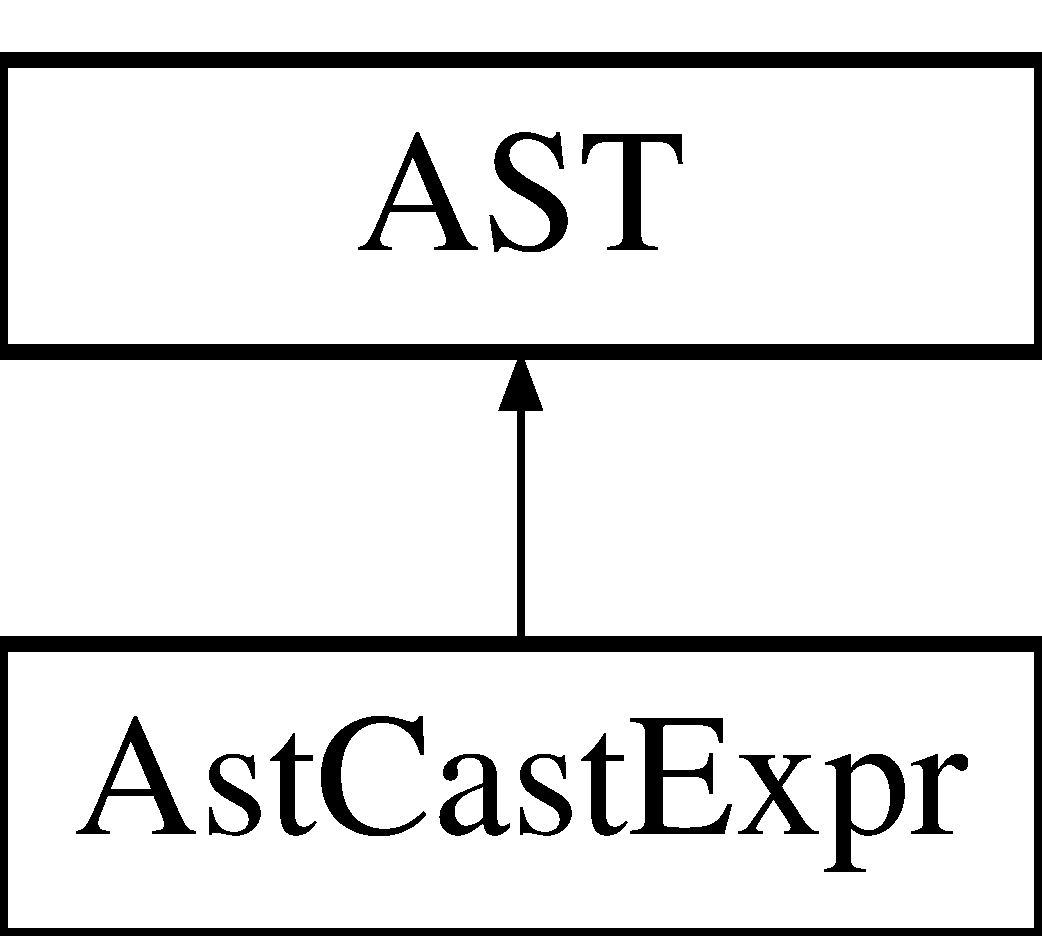
\includegraphics[height=2.000000cm]{classAstCastExpr}
\end{center}
\end{figure}
\subsection*{Public Member Functions}
\begin{DoxyCompactItemize}
\item 
\hypertarget{classAstCastExpr_a27857eebb48c3a153ddd4bebb0a5bc31}{{\bfseries Ast\-Cast\-Expr} (\hyperlink{classAstUnaryExpr}{Ast\-Unary\-Expr} $\ast$u)}\label{classAstCastExpr_a27857eebb48c3a153ddd4bebb0a5bc31}

\item 
\hypertarget{classAstCastExpr_a7a4384301ff0feb3c56fc6456792c416}{{\bfseries Ast\-Cast\-Expr} (\hyperlink{classAstTypeName}{Ast\-Type\-Name} $\ast$t, \hyperlink{classAstCastExpr}{Ast\-Cast\-Expr} $\ast$c)}\label{classAstCastExpr_a7a4384301ff0feb3c56fc6456792c416}

\item 
void \hyperlink{classAstCastExpr_a5c0f13da0e4bd315eb0e56c9cc9635e9}{Visit} ()
\begin{DoxyCompactList}\small\item\em This function is responsible for tree traversals. \end{DoxyCompactList}\item 
\hypertarget{classAstCastExpr_a27857eebb48c3a153ddd4bebb0a5bc31}{{\bfseries Ast\-Cast\-Expr} (\hyperlink{classAstUnaryExpr}{Ast\-Unary\-Expr} $\ast$u)}\label{classAstCastExpr_a27857eebb48c3a153ddd4bebb0a5bc31}

\item 
\hypertarget{classAstCastExpr_a7a4384301ff0feb3c56fc6456792c416}{{\bfseries Ast\-Cast\-Expr} (\hyperlink{classAstTypeName}{Ast\-Type\-Name} $\ast$t, \hyperlink{classAstCastExpr}{Ast\-Cast\-Expr} $\ast$c)}\label{classAstCastExpr_a7a4384301ff0feb3c56fc6456792c416}

\item 
void \hyperlink{classAstCastExpr_a5c0f13da0e4bd315eb0e56c9cc9635e9}{Visit} ()
\begin{DoxyCompactList}\small\item\em This function is responsible for tree traversals. \end{DoxyCompactList}\item 
\hypertarget{classAstCastExpr_a27857eebb48c3a153ddd4bebb0a5bc31}{{\bfseries Ast\-Cast\-Expr} (\hyperlink{classAstUnaryExpr}{Ast\-Unary\-Expr} $\ast$u)}\label{classAstCastExpr_a27857eebb48c3a153ddd4bebb0a5bc31}

\item 
\hypertarget{classAstCastExpr_a7a4384301ff0feb3c56fc6456792c416}{{\bfseries Ast\-Cast\-Expr} (\hyperlink{classAstTypeName}{Ast\-Type\-Name} $\ast$t, \hyperlink{classAstCastExpr}{Ast\-Cast\-Expr} $\ast$c)}\label{classAstCastExpr_a7a4384301ff0feb3c56fc6456792c416}

\item 
void \hyperlink{classAstCastExpr_a5c0f13da0e4bd315eb0e56c9cc9635e9}{Visit} ()
\begin{DoxyCompactList}\small\item\em This function is responsible for tree traversals. \end{DoxyCompactList}\item 
\hypertarget{classAstCastExpr_a27857eebb48c3a153ddd4bebb0a5bc31}{{\bfseries Ast\-Cast\-Expr} (\hyperlink{classAstUnaryExpr}{Ast\-Unary\-Expr} $\ast$u)}\label{classAstCastExpr_a27857eebb48c3a153ddd4bebb0a5bc31}

\item 
\hypertarget{classAstCastExpr_a7a4384301ff0feb3c56fc6456792c416}{{\bfseries Ast\-Cast\-Expr} (\hyperlink{classAstTypeName}{Ast\-Type\-Name} $\ast$t, \hyperlink{classAstCastExpr}{Ast\-Cast\-Expr} $\ast$c)}\label{classAstCastExpr_a7a4384301ff0feb3c56fc6456792c416}

\item 
void \hyperlink{classAstCastExpr_a5c0f13da0e4bd315eb0e56c9cc9635e9}{Visit} ()
\begin{DoxyCompactList}\small\item\em This function is responsible for tree traversals. \end{DoxyCompactList}\item 
void \hyperlink{classAST_a71d680856e95ff89f55d5311a552eba6}{set\-Label} (string l)
\begin{DoxyCompactList}\small\item\em Sets the label for the node. \end{DoxyCompactList}\item 
void \hyperlink{classAST_a71d680856e95ff89f55d5311a552eba6}{set\-Label} (string l)
\begin{DoxyCompactList}\small\item\em Sets the label for the node. \end{DoxyCompactList}\item 
void \hyperlink{classAST_a71d680856e95ff89f55d5311a552eba6}{set\-Label} (string l)
\begin{DoxyCompactList}\small\item\em Sets the label for the node. \end{DoxyCompactList}\item 
void \hyperlink{classAST_a71d680856e95ff89f55d5311a552eba6}{set\-Label} (string l)
\begin{DoxyCompactList}\small\item\em Sets the label for the node. \end{DoxyCompactList}\item 
int \hyperlink{classAST_ab7a5b1d9f1c2de0d98deb356f724a42c}{get\-U\-I\-D} ()
\begin{DoxyCompactList}\small\item\em Gets the node's unique I\-D. \end{DoxyCompactList}\item 
int \hyperlink{classAST_ab7a5b1d9f1c2de0d98deb356f724a42c}{get\-U\-I\-D} ()
\begin{DoxyCompactList}\small\item\em Gets the node's unique I\-D. \end{DoxyCompactList}\item 
int \hyperlink{classAST_ab7a5b1d9f1c2de0d98deb356f724a42c}{get\-U\-I\-D} ()
\begin{DoxyCompactList}\small\item\em Gets the node's unique I\-D. \end{DoxyCompactList}\item 
int \hyperlink{classAST_ab7a5b1d9f1c2de0d98deb356f724a42c}{get\-U\-I\-D} ()
\begin{DoxyCompactList}\small\item\em Gets the node's unique I\-D. \end{DoxyCompactList}\item 
string \hyperlink{classAST_aee029be902fffc927d16ccb03eb922ad}{get\-Label} ()
\begin{DoxyCompactList}\small\item\em Gets the node's label. \end{DoxyCompactList}\item 
string \hyperlink{classAST_aee029be902fffc927d16ccb03eb922ad}{get\-Label} ()
\begin{DoxyCompactList}\small\item\em Gets the node's label. \end{DoxyCompactList}\item 
string \hyperlink{classAST_aee029be902fffc927d16ccb03eb922ad}{get\-Label} ()
\begin{DoxyCompactList}\small\item\em Gets the node's label. \end{DoxyCompactList}\item 
string \hyperlink{classAST_aee029be902fffc927d16ccb03eb922ad}{get\-Label} ()
\begin{DoxyCompactList}\small\item\em Gets the node's label. \end{DoxyCompactList}\end{DoxyCompactItemize}
\subsection*{Public Attributes}
\begin{DoxyCompactItemize}
\item 
\hypertarget{classAstCastExpr_abcc1ebc0865a762524b5fc511a1184cb}{\hyperlink{classType}{Type} $\ast$ {\bfseries type}}\label{classAstCastExpr_abcc1ebc0865a762524b5fc511a1184cb}

\item 
\hypertarget{classAST_aaf215802de409f8096c063d01ffa6783}{bool \hyperlink{classAST_aaf215802de409f8096c063d01ffa6783}{needs\-Cast}}\label{classAST_aaf215802de409f8096c063d01ffa6783}

\begin{DoxyCompactList}\small\item\em This indicates if cast 3\-A\-C needs to be output, and is only relevant for expressions. \end{DoxyCompactList}\item 
\hypertarget{classAST_afa9e77ef650ec6664458fa6cb55be985}{bool \hyperlink{classAST_afa9e77ef650ec6664458fa6cb55be985}{is\-Conv}}\label{classAST_afa9e77ef650ec6664458fa6cb55be985}

\begin{DoxyCompactList}\small\item\em Indicates is a conversion is possible. \end{DoxyCompactList}\item 
\hypertarget{classAST_a61ef3317e023d45237e06615b387cd6b}{C\-O\-N\-V\-E\-R\-S\-I\-O\-N\-T\-Y\-P\-E \hyperlink{classAST_a61ef3317e023d45237e06615b387cd6b}{conv\-Type}}\label{classAST_a61ef3317e023d45237e06615b387cd6b}

\begin{DoxyCompactList}\small\item\em If needs\-Cast is true, then this indicates what the cast should be. \end{DoxyCompactList}\item 
\hypertarget{classAST_aea9b07b39d24183f38c0029cec0a878e}{int \hyperlink{classAST_aea9b07b39d24183f38c0029cec0a878e}{operand\-To\-Cast}}\label{classAST_aea9b07b39d24183f38c0029cec0a878e}

\begin{DoxyCompactList}\small\item\em This indicates if the first or second operand should be the one that is cast. \end{DoxyCompactList}\end{DoxyCompactItemize}
\subsection*{Static Public Attributes}
\begin{DoxyCompactItemize}
\item 
\hypertarget{classAST_a5fdfd5f7b104dd92889163bdadbc68d6}{static \hyperlink{classVisualizer}{Visualizer} \hyperlink{classAST_a5fdfd5f7b104dd92889163bdadbc68d6}{vis}}\label{classAST_a5fdfd5f7b104dd92889163bdadbc68d6}

\begin{DoxyCompactList}\small\item\em Static visualizer instance for generating the visualization of the \hyperlink{classAST}{A\-S\-T}. \end{DoxyCompactList}\item 
\hypertarget{classAST_a8a3ace322f50e030331065d644ee55ee}{static \hyperlink{classTAC__Generator}{T\-A\-C\-\_\-\-Generator} \hyperlink{classAST_a8a3ace322f50e030331065d644ee55ee}{tac\-Gen}}\label{classAST_a8a3ace322f50e030331065d644ee55ee}

\begin{DoxyCompactList}\small\item\em Three address code generator. \end{DoxyCompactList}\item 
\hypertarget{classAST_a1f69448c6dc368d005631a128460083d}{static string {\bfseries current\-Temp} =\char`\"{}\char`\"{}}\label{classAST_a1f69448c6dc368d005631a128460083d}

\item 
\hypertarget{classAST_a551aec090c932ab69365238b40a8a4eb}{static string \hyperlink{classAST_a551aec090c932ab69365238b40a8a4eb}{return\-Label} =\char`\"{}\char`\"{}}\label{classAST_a551aec090c932ab69365238b40a8a4eb}

\begin{DoxyCompactList}\small\item\em This is for storing the string id of any temporary result register that may be created during 3\-A\-C generation. \end{DoxyCompactList}\item 
\hypertarget{classAST_a73c0a266df52be71e6b527b6aa635173}{static list$<$ string $>$ {\bfseries temp\-Stack}}\label{classAST_a73c0a266df52be71e6b527b6aa635173}

\item 
\hypertarget{classAST_abf9e84b541ff04b7bb64e6e4371512d4}{static string {\bfseries last\-I\-D} =\char`\"{}\char`\"{}}\label{classAST_abf9e84b541ff04b7bb64e6e4371512d4}

\item 
\hypertarget{classAST_a163003bfe9c30510ec8039870346049f}{static \hyperlink{classSymTab}{Sym\-Tab} $\ast$ {\bfseries symbol\-Table} =N\-U\-L\-L}\label{classAST_a163003bfe9c30510ec8039870346049f}

\item 
\hypertarget{classAST_a5c3cc894d9c0453523dec9ed76f18a04}{static string {\bfseries current\-Function} =\char`\"{}\char`\"{}}\label{classAST_a5c3cc894d9c0453523dec9ed76f18a04}

\item 
\hypertarget{classAST_a66155513b59ff1a04c8ece8b20ec31f5}{static int {\bfseries current\-Constant\-Value} =0}\label{classAST_a66155513b59ff1a04c8ece8b20ec31f5}

\item 
\hypertarget{classAST_a3d031d7bab635ba1f015aade5943f40c}{static string {\bfseries current\-Id\-Name} =\char`\"{}\char`\"{}}\label{classAST_a3d031d7bab635ba1f015aade5943f40c}

\item 
\hypertarget{classAST_a16c4b6e54febc1a26b31a64a46972ef0}{static int {\bfseries current\-Index\-Val} = 0}\label{classAST_a16c4b6e54febc1a26b31a64a46972ef0}

\end{DoxyCompactItemize}
\subsection*{Protected Attributes}
\begin{DoxyCompactItemize}
\item 
\hypertarget{classAST_a847b778f1c3dd5a19de32de432ee6e15}{int \hyperlink{classAST_a847b778f1c3dd5a19de32de432ee6e15}{uid}}\label{classAST_a847b778f1c3dd5a19de32de432ee6e15}

\begin{DoxyCompactList}\small\item\em The unique id. \end{DoxyCompactList}\item 
\hypertarget{classAST_ab2e239ccc0688d2341724432ff5a1a31}{string \hyperlink{classAST_ab2e239ccc0688d2341724432ff5a1a31}{label}}\label{classAST_ab2e239ccc0688d2341724432ff5a1a31}

\begin{DoxyCompactList}\small\item\em The label to be printed in the visualization. \end{DoxyCompactList}\end{DoxyCompactItemize}
\subsection*{Private Attributes}
\begin{DoxyCompactItemize}
\item 
\hypertarget{classAstCastExpr_a4d5d3d510501ff9a55cab358323eeeaf}{\hyperlink{classAstUnaryExpr}{Ast\-Unary\-Expr} $\ast$ {\bfseries uniexpr}}\label{classAstCastExpr_a4d5d3d510501ff9a55cab358323eeeaf}

\item 
\hypertarget{classAstCastExpr_a8fbc1f5e844901bbeb9ad6784111ba51}{\hyperlink{classAstCastExpr}{Ast\-Cast\-Expr} $\ast$ {\bfseries cast}}\label{classAstCastExpr_a8fbc1f5e844901bbeb9ad6784111ba51}

\item 
\hypertarget{classAstCastExpr_affe29cc80bb5b579c7902916127efc50}{\hyperlink{classAstTypeName}{Ast\-Type\-Name} $\ast$ {\bfseries tname}}\label{classAstCastExpr_affe29cc80bb5b579c7902916127efc50}

\end{DoxyCompactItemize}


\subsection{Detailed Description}


Definition at line 460 of file Ast.\-h.



\subsection{Member Function Documentation}
\hypertarget{classAST_aee029be902fffc927d16ccb03eb922ad}{\index{Ast\-Cast\-Expr@{Ast\-Cast\-Expr}!get\-Label@{get\-Label}}
\index{get\-Label@{get\-Label}!AstCastExpr@{Ast\-Cast\-Expr}}
\subsubsection[{get\-Label}]{\setlength{\rightskip}{0pt plus 5cm}string A\-S\-T\-::get\-Label (
\begin{DoxyParamCaption}
{}
\end{DoxyParamCaption}
)\hspace{0.3cm}{\ttfamily [inline]}, {\ttfamily [inherited]}}}\label{classAST_aee029be902fffc927d16ccb03eb922ad}


Gets the node's label. 

\begin{DoxyReturn}{Returns}
The label 
\end{DoxyReturn}


Definition at line 60 of file Ast.\-h.

\hypertarget{classAST_aee029be902fffc927d16ccb03eb922ad}{\index{Ast\-Cast\-Expr@{Ast\-Cast\-Expr}!get\-Label@{get\-Label}}
\index{get\-Label@{get\-Label}!AstCastExpr@{Ast\-Cast\-Expr}}
\subsubsection[{get\-Label}]{\setlength{\rightskip}{0pt plus 5cm}string A\-S\-T\-::get\-Label (
\begin{DoxyParamCaption}
{}
\end{DoxyParamCaption}
)\hspace{0.3cm}{\ttfamily [inline]}, {\ttfamily [inherited]}}}\label{classAST_aee029be902fffc927d16ccb03eb922ad}


Gets the node's label. 

\begin{DoxyReturn}{Returns}
The label 
\end{DoxyReturn}


Definition at line 60 of file C\-Scanner.\-ll.

\hypertarget{classAST_aee029be902fffc927d16ccb03eb922ad}{\index{Ast\-Cast\-Expr@{Ast\-Cast\-Expr}!get\-Label@{get\-Label}}
\index{get\-Label@{get\-Label}!AstCastExpr@{Ast\-Cast\-Expr}}
\subsubsection[{get\-Label}]{\setlength{\rightskip}{0pt plus 5cm}string A\-S\-T\-::get\-Label (
\begin{DoxyParamCaption}
{}
\end{DoxyParamCaption}
)\hspace{0.3cm}{\ttfamily [inline]}, {\ttfamily [inherited]}}}\label{classAST_aee029be902fffc927d16ccb03eb922ad}


Gets the node's label. 

\begin{DoxyReturn}{Returns}
The label 
\end{DoxyReturn}


Definition at line 60 of file C\-Parser.\-yy.

\hypertarget{classAST_aee029be902fffc927d16ccb03eb922ad}{\index{Ast\-Cast\-Expr@{Ast\-Cast\-Expr}!get\-Label@{get\-Label}}
\index{get\-Label@{get\-Label}!AstCastExpr@{Ast\-Cast\-Expr}}
\subsubsection[{get\-Label}]{\setlength{\rightskip}{0pt plus 5cm}string A\-S\-T\-::get\-Label (
\begin{DoxyParamCaption}
{}
\end{DoxyParamCaption}
)\hspace{0.3cm}{\ttfamily [inline]}, {\ttfamily [inherited]}}}\label{classAST_aee029be902fffc927d16ccb03eb922ad}


Gets the node's label. 

\begin{DoxyReturn}{Returns}
The label 
\end{DoxyReturn}


Definition at line 60 of file C\-Parser.\-yy.

\hypertarget{classAST_ab7a5b1d9f1c2de0d98deb356f724a42c}{\index{Ast\-Cast\-Expr@{Ast\-Cast\-Expr}!get\-U\-I\-D@{get\-U\-I\-D}}
\index{get\-U\-I\-D@{get\-U\-I\-D}!AstCastExpr@{Ast\-Cast\-Expr}}
\subsubsection[{get\-U\-I\-D}]{\setlength{\rightskip}{0pt plus 5cm}int A\-S\-T\-::get\-U\-I\-D (
\begin{DoxyParamCaption}
{}
\end{DoxyParamCaption}
)\hspace{0.3cm}{\ttfamily [inline]}, {\ttfamily [inherited]}}}\label{classAST_ab7a5b1d9f1c2de0d98deb356f724a42c}


Gets the node's unique I\-D. 

\begin{DoxyReturn}{Returns}
The unique id 
\end{DoxyReturn}


Definition at line 53 of file C\-Parser.\-yy.

\hypertarget{classAST_ab7a5b1d9f1c2de0d98deb356f724a42c}{\index{Ast\-Cast\-Expr@{Ast\-Cast\-Expr}!get\-U\-I\-D@{get\-U\-I\-D}}
\index{get\-U\-I\-D@{get\-U\-I\-D}!AstCastExpr@{Ast\-Cast\-Expr}}
\subsubsection[{get\-U\-I\-D}]{\setlength{\rightskip}{0pt plus 5cm}int A\-S\-T\-::get\-U\-I\-D (
\begin{DoxyParamCaption}
{}
\end{DoxyParamCaption}
)\hspace{0.3cm}{\ttfamily [inline]}, {\ttfamily [inherited]}}}\label{classAST_ab7a5b1d9f1c2de0d98deb356f724a42c}


Gets the node's unique I\-D. 

\begin{DoxyReturn}{Returns}
The unique id 
\end{DoxyReturn}


Definition at line 53 of file C\-Parser.\-yy.

\hypertarget{classAST_ab7a5b1d9f1c2de0d98deb356f724a42c}{\index{Ast\-Cast\-Expr@{Ast\-Cast\-Expr}!get\-U\-I\-D@{get\-U\-I\-D}}
\index{get\-U\-I\-D@{get\-U\-I\-D}!AstCastExpr@{Ast\-Cast\-Expr}}
\subsubsection[{get\-U\-I\-D}]{\setlength{\rightskip}{0pt plus 5cm}int A\-S\-T\-::get\-U\-I\-D (
\begin{DoxyParamCaption}
{}
\end{DoxyParamCaption}
)\hspace{0.3cm}{\ttfamily [inline]}, {\ttfamily [inherited]}}}\label{classAST_ab7a5b1d9f1c2de0d98deb356f724a42c}


Gets the node's unique I\-D. 

\begin{DoxyReturn}{Returns}
The unique id 
\end{DoxyReturn}


Definition at line 53 of file C\-Scanner.\-ll.

\hypertarget{classAST_ab7a5b1d9f1c2de0d98deb356f724a42c}{\index{Ast\-Cast\-Expr@{Ast\-Cast\-Expr}!get\-U\-I\-D@{get\-U\-I\-D}}
\index{get\-U\-I\-D@{get\-U\-I\-D}!AstCastExpr@{Ast\-Cast\-Expr}}
\subsubsection[{get\-U\-I\-D}]{\setlength{\rightskip}{0pt plus 5cm}int A\-S\-T\-::get\-U\-I\-D (
\begin{DoxyParamCaption}
{}
\end{DoxyParamCaption}
)\hspace{0.3cm}{\ttfamily [inline]}, {\ttfamily [inherited]}}}\label{classAST_ab7a5b1d9f1c2de0d98deb356f724a42c}


Gets the node's unique I\-D. 

\begin{DoxyReturn}{Returns}
The unique id 
\end{DoxyReturn}


Definition at line 53 of file Ast.\-h.

\hypertarget{classAST_a71d680856e95ff89f55d5311a552eba6}{\index{Ast\-Cast\-Expr@{Ast\-Cast\-Expr}!set\-Label@{set\-Label}}
\index{set\-Label@{set\-Label}!AstCastExpr@{Ast\-Cast\-Expr}}
\subsubsection[{set\-Label}]{\setlength{\rightskip}{0pt plus 5cm}void A\-S\-T\-::set\-Label (
\begin{DoxyParamCaption}
\item[{string}]{l}
\end{DoxyParamCaption}
)\hspace{0.3cm}{\ttfamily [inline]}, {\ttfamily [inherited]}}}\label{classAST_a71d680856e95ff89f55d5311a552eba6}


Sets the label for the node. 


\begin{DoxyParams}{Parameters}
{\em l} & The label string \\
\hline
\end{DoxyParams}


Definition at line 43 of file C\-Scanner.\-ll.

\hypertarget{classAST_a71d680856e95ff89f55d5311a552eba6}{\index{Ast\-Cast\-Expr@{Ast\-Cast\-Expr}!set\-Label@{set\-Label}}
\index{set\-Label@{set\-Label}!AstCastExpr@{Ast\-Cast\-Expr}}
\subsubsection[{set\-Label}]{\setlength{\rightskip}{0pt plus 5cm}void A\-S\-T\-::set\-Label (
\begin{DoxyParamCaption}
\item[{string}]{l}
\end{DoxyParamCaption}
)\hspace{0.3cm}{\ttfamily [inline]}, {\ttfamily [inherited]}}}\label{classAST_a71d680856e95ff89f55d5311a552eba6}


Sets the label for the node. 


\begin{DoxyParams}{Parameters}
{\em l} & The label string \\
\hline
\end{DoxyParams}


Definition at line 43 of file C\-Parser.\-yy.

\hypertarget{classAST_a71d680856e95ff89f55d5311a552eba6}{\index{Ast\-Cast\-Expr@{Ast\-Cast\-Expr}!set\-Label@{set\-Label}}
\index{set\-Label@{set\-Label}!AstCastExpr@{Ast\-Cast\-Expr}}
\subsubsection[{set\-Label}]{\setlength{\rightskip}{0pt plus 5cm}void A\-S\-T\-::set\-Label (
\begin{DoxyParamCaption}
\item[{string}]{l}
\end{DoxyParamCaption}
)\hspace{0.3cm}{\ttfamily [inline]}, {\ttfamily [inherited]}}}\label{classAST_a71d680856e95ff89f55d5311a552eba6}


Sets the label for the node. 


\begin{DoxyParams}{Parameters}
{\em l} & The label string \\
\hline
\end{DoxyParams}


Definition at line 43 of file Ast.\-h.

\hypertarget{classAST_a71d680856e95ff89f55d5311a552eba6}{\index{Ast\-Cast\-Expr@{Ast\-Cast\-Expr}!set\-Label@{set\-Label}}
\index{set\-Label@{set\-Label}!AstCastExpr@{Ast\-Cast\-Expr}}
\subsubsection[{set\-Label}]{\setlength{\rightskip}{0pt plus 5cm}void A\-S\-T\-::set\-Label (
\begin{DoxyParamCaption}
\item[{string}]{l}
\end{DoxyParamCaption}
)\hspace{0.3cm}{\ttfamily [inline]}, {\ttfamily [inherited]}}}\label{classAST_a71d680856e95ff89f55d5311a552eba6}


Sets the label for the node. 


\begin{DoxyParams}{Parameters}
{\em l} & The label string \\
\hline
\end{DoxyParams}


Definition at line 43 of file C\-Parser.\-yy.

\hypertarget{classAstCastExpr_a5c0f13da0e4bd315eb0e56c9cc9635e9}{\index{Ast\-Cast\-Expr@{Ast\-Cast\-Expr}!Visit@{Visit}}
\index{Visit@{Visit}!AstCastExpr@{Ast\-Cast\-Expr}}
\subsubsection[{Visit}]{\setlength{\rightskip}{0pt plus 5cm}void Ast\-Cast\-Expr\-::\-Visit (
\begin{DoxyParamCaption}
{}
\end{DoxyParamCaption}
)\hspace{0.3cm}{\ttfamily [virtual]}}}\label{classAstCastExpr_a5c0f13da0e4bd315eb0e56c9cc9635e9}


This function is responsible for tree traversals. 

This function will call the Visit functions of each of it's children nodes, call the visualization code for itself, and output any 3\-A\-C that can be generated at the current node. 

Reimplemented from \hyperlink{classAST_a5828cc86f2c4f1a0aeab6d7069e8fd82}{A\-S\-T}.



Definition at line 748 of file Ast.\-cpp.

\hypertarget{classAstCastExpr_a5c0f13da0e4bd315eb0e56c9cc9635e9}{\index{Ast\-Cast\-Expr@{Ast\-Cast\-Expr}!Visit@{Visit}}
\index{Visit@{Visit}!AstCastExpr@{Ast\-Cast\-Expr}}
\subsubsection[{Visit}]{\setlength{\rightskip}{0pt plus 5cm}void Ast\-Cast\-Expr\-::\-Visit (
\begin{DoxyParamCaption}
{}
\end{DoxyParamCaption}
)\hspace{0.3cm}{\ttfamily [virtual]}}}\label{classAstCastExpr_a5c0f13da0e4bd315eb0e56c9cc9635e9}


This function is responsible for tree traversals. 

This function will call the Visit functions of each of it's children nodes, call the visualization code for itself, and output any 3\-A\-C that can be generated at the current node. 

Reimplemented from \hyperlink{classAST_a5828cc86f2c4f1a0aeab6d7069e8fd82}{A\-S\-T}.

\hypertarget{classAstCastExpr_a5c0f13da0e4bd315eb0e56c9cc9635e9}{\index{Ast\-Cast\-Expr@{Ast\-Cast\-Expr}!Visit@{Visit}}
\index{Visit@{Visit}!AstCastExpr@{Ast\-Cast\-Expr}}
\subsubsection[{Visit}]{\setlength{\rightskip}{0pt plus 5cm}void Ast\-Cast\-Expr\-::\-Visit (
\begin{DoxyParamCaption}
{}
\end{DoxyParamCaption}
)\hspace{0.3cm}{\ttfamily [virtual]}}}\label{classAstCastExpr_a5c0f13da0e4bd315eb0e56c9cc9635e9}


This function is responsible for tree traversals. 

This function will call the Visit functions of each of it's children nodes, call the visualization code for itself, and output any 3\-A\-C that can be generated at the current node. 

Reimplemented from \hyperlink{classAST_a5828cc86f2c4f1a0aeab6d7069e8fd82}{A\-S\-T}.

\hypertarget{classAstCastExpr_a5c0f13da0e4bd315eb0e56c9cc9635e9}{\index{Ast\-Cast\-Expr@{Ast\-Cast\-Expr}!Visit@{Visit}}
\index{Visit@{Visit}!AstCastExpr@{Ast\-Cast\-Expr}}
\subsubsection[{Visit}]{\setlength{\rightskip}{0pt plus 5cm}void Ast\-Cast\-Expr\-::\-Visit (
\begin{DoxyParamCaption}
{}
\end{DoxyParamCaption}
)\hspace{0.3cm}{\ttfamily [virtual]}}}\label{classAstCastExpr_a5c0f13da0e4bd315eb0e56c9cc9635e9}


This function is responsible for tree traversals. 

This function will call the Visit functions of each of it's children nodes, call the visualization code for itself, and output any 3\-A\-C that can be generated at the current node. 

Reimplemented from \hyperlink{classAST_a5828cc86f2c4f1a0aeab6d7069e8fd82}{A\-S\-T}.



The documentation for this class was generated from the following files\-:\begin{DoxyCompactItemize}
\item 
Ast.\-h\item 
Ast.\-cpp\end{DoxyCompactItemize}

\hypertarget{classAstCompoundStmt}{\section{Ast\-Compound\-Stmt Class Reference}
\label{classAstCompoundStmt}\index{Ast\-Compound\-Stmt@{Ast\-Compound\-Stmt}}
}
Inheritance diagram for Ast\-Compound\-Stmt\-:\begin{figure}[H]
\begin{center}
\leavevmode
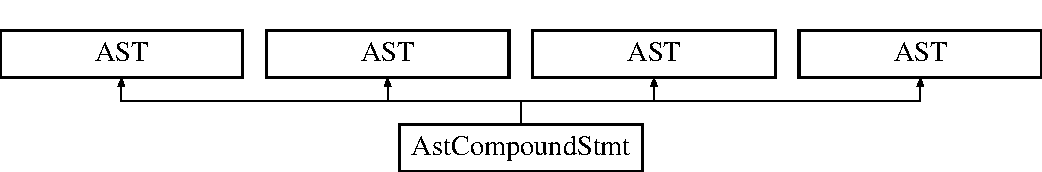
\includegraphics[height=2.000000cm]{classAstCompoundStmt}
\end{center}
\end{figure}
\subsection*{Public Member Functions}
\begin{DoxyCompactItemize}
\item 
\hypertarget{classAstCompoundStmt_af9005e930ed909289b88f84f9c7dffc1}{{\bfseries Ast\-Compound\-Stmt} (\hyperlink{classAstDeclarationList}{Ast\-Declaration\-List} $\ast$d, \hyperlink{classAstStatementList}{Ast\-Statement\-List} $\ast$s)}\label{classAstCompoundStmt_af9005e930ed909289b88f84f9c7dffc1}

\item 
void \hyperlink{classAstCompoundStmt_a6ff97b453379db290afe4c4c17ad5244}{Visit} ()
\begin{DoxyCompactList}\small\item\em This function is responsible for tree traversals. \end{DoxyCompactList}\item 
\hypertarget{classAstCompoundStmt_af9005e930ed909289b88f84f9c7dffc1}{{\bfseries Ast\-Compound\-Stmt} (\hyperlink{classAstDeclarationList}{Ast\-Declaration\-List} $\ast$d, \hyperlink{classAstStatementList}{Ast\-Statement\-List} $\ast$s)}\label{classAstCompoundStmt_af9005e930ed909289b88f84f9c7dffc1}

\item 
void \hyperlink{classAstCompoundStmt_a6ff97b453379db290afe4c4c17ad5244}{Visit} ()
\begin{DoxyCompactList}\small\item\em This function is responsible for tree traversals. \end{DoxyCompactList}\item 
\hypertarget{classAstCompoundStmt_af9005e930ed909289b88f84f9c7dffc1}{{\bfseries Ast\-Compound\-Stmt} (\hyperlink{classAstDeclarationList}{Ast\-Declaration\-List} $\ast$d, \hyperlink{classAstStatementList}{Ast\-Statement\-List} $\ast$s)}\label{classAstCompoundStmt_af9005e930ed909289b88f84f9c7dffc1}

\item 
void \hyperlink{classAstCompoundStmt_a6ff97b453379db290afe4c4c17ad5244}{Visit} ()
\begin{DoxyCompactList}\small\item\em This function is responsible for tree traversals. \end{DoxyCompactList}\item 
\hypertarget{classAstCompoundStmt_af9005e930ed909289b88f84f9c7dffc1}{{\bfseries Ast\-Compound\-Stmt} (\hyperlink{classAstDeclarationList}{Ast\-Declaration\-List} $\ast$d, \hyperlink{classAstStatementList}{Ast\-Statement\-List} $\ast$s)}\label{classAstCompoundStmt_af9005e930ed909289b88f84f9c7dffc1}

\item 
void \hyperlink{classAstCompoundStmt_a6ff97b453379db290afe4c4c17ad5244}{Visit} ()
\begin{DoxyCompactList}\small\item\em This function is responsible for tree traversals. \end{DoxyCompactList}\item 
void \hyperlink{classAST_a71d680856e95ff89f55d5311a552eba6}{set\-Label} (string l)
\begin{DoxyCompactList}\small\item\em Sets the label for the node. \end{DoxyCompactList}\item 
void \hyperlink{classAST_a71d680856e95ff89f55d5311a552eba6}{set\-Label} (string l)
\begin{DoxyCompactList}\small\item\em Sets the label for the node. \end{DoxyCompactList}\item 
void \hyperlink{classAST_a71d680856e95ff89f55d5311a552eba6}{set\-Label} (string l)
\begin{DoxyCompactList}\small\item\em Sets the label for the node. \end{DoxyCompactList}\item 
void \hyperlink{classAST_a71d680856e95ff89f55d5311a552eba6}{set\-Label} (string l)
\begin{DoxyCompactList}\small\item\em Sets the label for the node. \end{DoxyCompactList}\item 
int \hyperlink{classAST_ab7a5b1d9f1c2de0d98deb356f724a42c}{get\-U\-I\-D} ()
\begin{DoxyCompactList}\small\item\em Gets the node's unique I\-D. \end{DoxyCompactList}\item 
int \hyperlink{classAST_ab7a5b1d9f1c2de0d98deb356f724a42c}{get\-U\-I\-D} ()
\begin{DoxyCompactList}\small\item\em Gets the node's unique I\-D. \end{DoxyCompactList}\item 
int \hyperlink{classAST_ab7a5b1d9f1c2de0d98deb356f724a42c}{get\-U\-I\-D} ()
\begin{DoxyCompactList}\small\item\em Gets the node's unique I\-D. \end{DoxyCompactList}\item 
int \hyperlink{classAST_ab7a5b1d9f1c2de0d98deb356f724a42c}{get\-U\-I\-D} ()
\begin{DoxyCompactList}\small\item\em Gets the node's unique I\-D. \end{DoxyCompactList}\item 
string \hyperlink{classAST_aee029be902fffc927d16ccb03eb922ad}{get\-Label} ()
\begin{DoxyCompactList}\small\item\em Gets the node's label. \end{DoxyCompactList}\item 
string \hyperlink{classAST_aee029be902fffc927d16ccb03eb922ad}{get\-Label} ()
\begin{DoxyCompactList}\small\item\em Gets the node's label. \end{DoxyCompactList}\item 
string \hyperlink{classAST_aee029be902fffc927d16ccb03eb922ad}{get\-Label} ()
\begin{DoxyCompactList}\small\item\em Gets the node's label. \end{DoxyCompactList}\item 
string \hyperlink{classAST_aee029be902fffc927d16ccb03eb922ad}{get\-Label} ()
\begin{DoxyCompactList}\small\item\em Gets the node's label. \end{DoxyCompactList}\end{DoxyCompactItemize}
\subsection*{Public Attributes}
\begin{DoxyCompactItemize}
\item 
\hypertarget{classAST_aaf215802de409f8096c063d01ffa6783}{bool \hyperlink{classAST_aaf215802de409f8096c063d01ffa6783}{needs\-Cast}}\label{classAST_aaf215802de409f8096c063d01ffa6783}

\begin{DoxyCompactList}\small\item\em This indicates if cast 3\-A\-C needs to be output, and is only relevant for expressions. \end{DoxyCompactList}\item 
\hypertarget{classAST_afa9e77ef650ec6664458fa6cb55be985}{bool \hyperlink{classAST_afa9e77ef650ec6664458fa6cb55be985}{is\-Conv}}\label{classAST_afa9e77ef650ec6664458fa6cb55be985}

\begin{DoxyCompactList}\small\item\em Indicates is a conversion is possible. \end{DoxyCompactList}\item 
\hypertarget{classAST_a61ef3317e023d45237e06615b387cd6b}{C\-O\-N\-V\-E\-R\-S\-I\-O\-N\-T\-Y\-P\-E \hyperlink{classAST_a61ef3317e023d45237e06615b387cd6b}{conv\-Type}}\label{classAST_a61ef3317e023d45237e06615b387cd6b}

\begin{DoxyCompactList}\small\item\em If needs\-Cast is true, then this indicates what the cast should be. \end{DoxyCompactList}\item 
\hypertarget{classAST_aea9b07b39d24183f38c0029cec0a878e}{int \hyperlink{classAST_aea9b07b39d24183f38c0029cec0a878e}{operand\-To\-Cast}}\label{classAST_aea9b07b39d24183f38c0029cec0a878e}

\begin{DoxyCompactList}\small\item\em This indicates if the first or second operand should be the one that is cast. \end{DoxyCompactList}\end{DoxyCompactItemize}
\subsection*{Static Public Attributes}
\begin{DoxyCompactItemize}
\item 
\hypertarget{classAST_a5fdfd5f7b104dd92889163bdadbc68d6}{static \hyperlink{classVisualizer}{Visualizer} \hyperlink{classAST_a5fdfd5f7b104dd92889163bdadbc68d6}{vis}}\label{classAST_a5fdfd5f7b104dd92889163bdadbc68d6}

\begin{DoxyCompactList}\small\item\em Static visualizer instance for generating the visualization of the \hyperlink{classAST}{A\-S\-T}. \end{DoxyCompactList}\item 
\hypertarget{classAST_a8a3ace322f50e030331065d644ee55ee}{static \hyperlink{classTAC__Generator}{T\-A\-C\-\_\-\-Generator} \hyperlink{classAST_a8a3ace322f50e030331065d644ee55ee}{tac\-Gen}}\label{classAST_a8a3ace322f50e030331065d644ee55ee}

\begin{DoxyCompactList}\small\item\em Three address code generator. \end{DoxyCompactList}\item 
\hypertarget{classAST_a1f69448c6dc368d005631a128460083d}{static string {\bfseries current\-Temp} =\char`\"{}\char`\"{}}\label{classAST_a1f69448c6dc368d005631a128460083d}

\item 
\hypertarget{classAST_a551aec090c932ab69365238b40a8a4eb}{static string \hyperlink{classAST_a551aec090c932ab69365238b40a8a4eb}{return\-Label} =\char`\"{}\char`\"{}}\label{classAST_a551aec090c932ab69365238b40a8a4eb}

\begin{DoxyCompactList}\small\item\em This is for storing the string id of any temporary result register that may be created during 3\-A\-C generation. \end{DoxyCompactList}\item 
\hypertarget{classAST_a73c0a266df52be71e6b527b6aa635173}{static list$<$ string $>$ {\bfseries temp\-Stack}}\label{classAST_a73c0a266df52be71e6b527b6aa635173}

\item 
\hypertarget{classAST_abf9e84b541ff04b7bb64e6e4371512d4}{static string {\bfseries last\-I\-D} =\char`\"{}\char`\"{}}\label{classAST_abf9e84b541ff04b7bb64e6e4371512d4}

\item 
\hypertarget{classAST_a163003bfe9c30510ec8039870346049f}{static \hyperlink{classSymTab}{Sym\-Tab} $\ast$ {\bfseries symbol\-Table} =N\-U\-L\-L}\label{classAST_a163003bfe9c30510ec8039870346049f}

\item 
\hypertarget{classAST_a5c3cc894d9c0453523dec9ed76f18a04}{static string {\bfseries current\-Function} =\char`\"{}\char`\"{}}\label{classAST_a5c3cc894d9c0453523dec9ed76f18a04}

\end{DoxyCompactItemize}
\subsection*{Protected Attributes}
\begin{DoxyCompactItemize}
\item 
\hypertarget{classAST_a847b778f1c3dd5a19de32de432ee6e15}{int \hyperlink{classAST_a847b778f1c3dd5a19de32de432ee6e15}{uid}}\label{classAST_a847b778f1c3dd5a19de32de432ee6e15}

\begin{DoxyCompactList}\small\item\em The unique id. \end{DoxyCompactList}\item 
\hypertarget{classAST_ab2e239ccc0688d2341724432ff5a1a31}{string \hyperlink{classAST_ab2e239ccc0688d2341724432ff5a1a31}{label}}\label{classAST_ab2e239ccc0688d2341724432ff5a1a31}

\begin{DoxyCompactList}\small\item\em The label to be printed in the visualization. \end{DoxyCompactList}\end{DoxyCompactItemize}
\subsection*{Private Attributes}
\begin{DoxyCompactItemize}
\item 
\hypertarget{classAstCompoundStmt_a8d3300ea92e3312aaf374a570fe66946}{\hyperlink{classAstStatementList}{Ast\-Statement\-List} $\ast$ {\bfseries stmt\-List}}\label{classAstCompoundStmt_a8d3300ea92e3312aaf374a570fe66946}

\item 
\hypertarget{classAstCompoundStmt_a5b0dc6bae31ec73ed26155fe682d7ac1}{\hyperlink{classAstDeclarationList}{Ast\-Declaration\-List} $\ast$ {\bfseries decl\-List}}\label{classAstCompoundStmt_a5b0dc6bae31ec73ed26155fe682d7ac1}

\end{DoxyCompactItemize}


\subsection{Detailed Description}


Definition at line 794 of file Ast.\-h.



\subsection{Member Function Documentation}
\hypertarget{classAST_aee029be902fffc927d16ccb03eb922ad}{\index{Ast\-Compound\-Stmt@{Ast\-Compound\-Stmt}!get\-Label@{get\-Label}}
\index{get\-Label@{get\-Label}!AstCompoundStmt@{Ast\-Compound\-Stmt}}
\subsubsection[{get\-Label}]{\setlength{\rightskip}{0pt plus 5cm}string A\-S\-T\-::get\-Label (
\begin{DoxyParamCaption}
{}
\end{DoxyParamCaption}
)\hspace{0.3cm}{\ttfamily [inline]}, {\ttfamily [inherited]}}}\label{classAST_aee029be902fffc927d16ccb03eb922ad}


Gets the node's label. 

\begin{DoxyReturn}{Returns}
The label 
\end{DoxyReturn}


Definition at line 60 of file Ast.\-h.

\hypertarget{classAST_aee029be902fffc927d16ccb03eb922ad}{\index{Ast\-Compound\-Stmt@{Ast\-Compound\-Stmt}!get\-Label@{get\-Label}}
\index{get\-Label@{get\-Label}!AstCompoundStmt@{Ast\-Compound\-Stmt}}
\subsubsection[{get\-Label}]{\setlength{\rightskip}{0pt plus 5cm}string A\-S\-T\-::get\-Label (
\begin{DoxyParamCaption}
{}
\end{DoxyParamCaption}
)\hspace{0.3cm}{\ttfamily [inline]}, {\ttfamily [inherited]}}}\label{classAST_aee029be902fffc927d16ccb03eb922ad}


Gets the node's label. 

\begin{DoxyReturn}{Returns}
The label 
\end{DoxyReturn}


Definition at line 60 of file C\-Scanner.\-ll.

\hypertarget{classAST_aee029be902fffc927d16ccb03eb922ad}{\index{Ast\-Compound\-Stmt@{Ast\-Compound\-Stmt}!get\-Label@{get\-Label}}
\index{get\-Label@{get\-Label}!AstCompoundStmt@{Ast\-Compound\-Stmt}}
\subsubsection[{get\-Label}]{\setlength{\rightskip}{0pt plus 5cm}string A\-S\-T\-::get\-Label (
\begin{DoxyParamCaption}
{}
\end{DoxyParamCaption}
)\hspace{0.3cm}{\ttfamily [inline]}, {\ttfamily [inherited]}}}\label{classAST_aee029be902fffc927d16ccb03eb922ad}


Gets the node's label. 

\begin{DoxyReturn}{Returns}
The label 
\end{DoxyReturn}


Definition at line 60 of file C\-Parser.\-yy.

\hypertarget{classAST_aee029be902fffc927d16ccb03eb922ad}{\index{Ast\-Compound\-Stmt@{Ast\-Compound\-Stmt}!get\-Label@{get\-Label}}
\index{get\-Label@{get\-Label}!AstCompoundStmt@{Ast\-Compound\-Stmt}}
\subsubsection[{get\-Label}]{\setlength{\rightskip}{0pt plus 5cm}string A\-S\-T\-::get\-Label (
\begin{DoxyParamCaption}
{}
\end{DoxyParamCaption}
)\hspace{0.3cm}{\ttfamily [inline]}, {\ttfamily [inherited]}}}\label{classAST_aee029be902fffc927d16ccb03eb922ad}


Gets the node's label. 

\begin{DoxyReturn}{Returns}
The label 
\end{DoxyReturn}


Definition at line 60 of file C\-Parser.\-yy.

\hypertarget{classAST_ab7a5b1d9f1c2de0d98deb356f724a42c}{\index{Ast\-Compound\-Stmt@{Ast\-Compound\-Stmt}!get\-U\-I\-D@{get\-U\-I\-D}}
\index{get\-U\-I\-D@{get\-U\-I\-D}!AstCompoundStmt@{Ast\-Compound\-Stmt}}
\subsubsection[{get\-U\-I\-D}]{\setlength{\rightskip}{0pt plus 5cm}int A\-S\-T\-::get\-U\-I\-D (
\begin{DoxyParamCaption}
{}
\end{DoxyParamCaption}
)\hspace{0.3cm}{\ttfamily [inline]}, {\ttfamily [inherited]}}}\label{classAST_ab7a5b1d9f1c2de0d98deb356f724a42c}


Gets the node's unique I\-D. 

\begin{DoxyReturn}{Returns}
The unique id 
\end{DoxyReturn}


Definition at line 53 of file C\-Parser.\-yy.

\hypertarget{classAST_ab7a5b1d9f1c2de0d98deb356f724a42c}{\index{Ast\-Compound\-Stmt@{Ast\-Compound\-Stmt}!get\-U\-I\-D@{get\-U\-I\-D}}
\index{get\-U\-I\-D@{get\-U\-I\-D}!AstCompoundStmt@{Ast\-Compound\-Stmt}}
\subsubsection[{get\-U\-I\-D}]{\setlength{\rightskip}{0pt plus 5cm}int A\-S\-T\-::get\-U\-I\-D (
\begin{DoxyParamCaption}
{}
\end{DoxyParamCaption}
)\hspace{0.3cm}{\ttfamily [inline]}, {\ttfamily [inherited]}}}\label{classAST_ab7a5b1d9f1c2de0d98deb356f724a42c}


Gets the node's unique I\-D. 

\begin{DoxyReturn}{Returns}
The unique id 
\end{DoxyReturn}


Definition at line 53 of file C\-Parser.\-yy.

\hypertarget{classAST_ab7a5b1d9f1c2de0d98deb356f724a42c}{\index{Ast\-Compound\-Stmt@{Ast\-Compound\-Stmt}!get\-U\-I\-D@{get\-U\-I\-D}}
\index{get\-U\-I\-D@{get\-U\-I\-D}!AstCompoundStmt@{Ast\-Compound\-Stmt}}
\subsubsection[{get\-U\-I\-D}]{\setlength{\rightskip}{0pt plus 5cm}int A\-S\-T\-::get\-U\-I\-D (
\begin{DoxyParamCaption}
{}
\end{DoxyParamCaption}
)\hspace{0.3cm}{\ttfamily [inline]}, {\ttfamily [inherited]}}}\label{classAST_ab7a5b1d9f1c2de0d98deb356f724a42c}


Gets the node's unique I\-D. 

\begin{DoxyReturn}{Returns}
The unique id 
\end{DoxyReturn}


Definition at line 53 of file C\-Scanner.\-ll.

\hypertarget{classAST_ab7a5b1d9f1c2de0d98deb356f724a42c}{\index{Ast\-Compound\-Stmt@{Ast\-Compound\-Stmt}!get\-U\-I\-D@{get\-U\-I\-D}}
\index{get\-U\-I\-D@{get\-U\-I\-D}!AstCompoundStmt@{Ast\-Compound\-Stmt}}
\subsubsection[{get\-U\-I\-D}]{\setlength{\rightskip}{0pt plus 5cm}int A\-S\-T\-::get\-U\-I\-D (
\begin{DoxyParamCaption}
{}
\end{DoxyParamCaption}
)\hspace{0.3cm}{\ttfamily [inline]}, {\ttfamily [inherited]}}}\label{classAST_ab7a5b1d9f1c2de0d98deb356f724a42c}


Gets the node's unique I\-D. 

\begin{DoxyReturn}{Returns}
The unique id 
\end{DoxyReturn}


Definition at line 53 of file Ast.\-h.

\hypertarget{classAST_a71d680856e95ff89f55d5311a552eba6}{\index{Ast\-Compound\-Stmt@{Ast\-Compound\-Stmt}!set\-Label@{set\-Label}}
\index{set\-Label@{set\-Label}!AstCompoundStmt@{Ast\-Compound\-Stmt}}
\subsubsection[{set\-Label}]{\setlength{\rightskip}{0pt plus 5cm}void A\-S\-T\-::set\-Label (
\begin{DoxyParamCaption}
\item[{string}]{l}
\end{DoxyParamCaption}
)\hspace{0.3cm}{\ttfamily [inline]}, {\ttfamily [inherited]}}}\label{classAST_a71d680856e95ff89f55d5311a552eba6}


Sets the label for the node. 


\begin{DoxyParams}{Parameters}
{\em l} & The label string \\
\hline
\end{DoxyParams}


Definition at line 43 of file C\-Scanner.\-ll.

\hypertarget{classAST_a71d680856e95ff89f55d5311a552eba6}{\index{Ast\-Compound\-Stmt@{Ast\-Compound\-Stmt}!set\-Label@{set\-Label}}
\index{set\-Label@{set\-Label}!AstCompoundStmt@{Ast\-Compound\-Stmt}}
\subsubsection[{set\-Label}]{\setlength{\rightskip}{0pt plus 5cm}void A\-S\-T\-::set\-Label (
\begin{DoxyParamCaption}
\item[{string}]{l}
\end{DoxyParamCaption}
)\hspace{0.3cm}{\ttfamily [inline]}, {\ttfamily [inherited]}}}\label{classAST_a71d680856e95ff89f55d5311a552eba6}


Sets the label for the node. 


\begin{DoxyParams}{Parameters}
{\em l} & The label string \\
\hline
\end{DoxyParams}


Definition at line 43 of file C\-Parser.\-yy.

\hypertarget{classAST_a71d680856e95ff89f55d5311a552eba6}{\index{Ast\-Compound\-Stmt@{Ast\-Compound\-Stmt}!set\-Label@{set\-Label}}
\index{set\-Label@{set\-Label}!AstCompoundStmt@{Ast\-Compound\-Stmt}}
\subsubsection[{set\-Label}]{\setlength{\rightskip}{0pt plus 5cm}void A\-S\-T\-::set\-Label (
\begin{DoxyParamCaption}
\item[{string}]{l}
\end{DoxyParamCaption}
)\hspace{0.3cm}{\ttfamily [inline]}, {\ttfamily [inherited]}}}\label{classAST_a71d680856e95ff89f55d5311a552eba6}


Sets the label for the node. 


\begin{DoxyParams}{Parameters}
{\em l} & The label string \\
\hline
\end{DoxyParams}


Definition at line 43 of file Ast.\-h.

\hypertarget{classAST_a71d680856e95ff89f55d5311a552eba6}{\index{Ast\-Compound\-Stmt@{Ast\-Compound\-Stmt}!set\-Label@{set\-Label}}
\index{set\-Label@{set\-Label}!AstCompoundStmt@{Ast\-Compound\-Stmt}}
\subsubsection[{set\-Label}]{\setlength{\rightskip}{0pt plus 5cm}void A\-S\-T\-::set\-Label (
\begin{DoxyParamCaption}
\item[{string}]{l}
\end{DoxyParamCaption}
)\hspace{0.3cm}{\ttfamily [inline]}, {\ttfamily [inherited]}}}\label{classAST_a71d680856e95ff89f55d5311a552eba6}


Sets the label for the node. 


\begin{DoxyParams}{Parameters}
{\em l} & The label string \\
\hline
\end{DoxyParams}


Definition at line 43 of file C\-Parser.\-yy.

\hypertarget{classAstCompoundStmt_a6ff97b453379db290afe4c4c17ad5244}{\index{Ast\-Compound\-Stmt@{Ast\-Compound\-Stmt}!Visit@{Visit}}
\index{Visit@{Visit}!AstCompoundStmt@{Ast\-Compound\-Stmt}}
\subsubsection[{Visit}]{\setlength{\rightskip}{0pt plus 5cm}void Ast\-Compound\-Stmt\-::\-Visit (
\begin{DoxyParamCaption}
{}
\end{DoxyParamCaption}
)\hspace{0.3cm}{\ttfamily [virtual]}}}\label{classAstCompoundStmt_a6ff97b453379db290afe4c4c17ad5244}


This function is responsible for tree traversals. 

This function will call the Visit functions of each of it's children nodes, call the visualization code for itself, and output any 3\-A\-C that can be generated at the current node. 

Reimplemented from \hyperlink{classAST_a5828cc86f2c4f1a0aeab6d7069e8fd82}{A\-S\-T}.



Definition at line 2443 of file Ast.\-cpp.

\hypertarget{classAstCompoundStmt_a6ff97b453379db290afe4c4c17ad5244}{\index{Ast\-Compound\-Stmt@{Ast\-Compound\-Stmt}!Visit@{Visit}}
\index{Visit@{Visit}!AstCompoundStmt@{Ast\-Compound\-Stmt}}
\subsubsection[{Visit}]{\setlength{\rightskip}{0pt plus 5cm}void Ast\-Compound\-Stmt\-::\-Visit (
\begin{DoxyParamCaption}
{}
\end{DoxyParamCaption}
)\hspace{0.3cm}{\ttfamily [virtual]}}}\label{classAstCompoundStmt_a6ff97b453379db290afe4c4c17ad5244}


This function is responsible for tree traversals. 

This function will call the Visit functions of each of it's children nodes, call the visualization code for itself, and output any 3\-A\-C that can be generated at the current node. 

Reimplemented from \hyperlink{classAST_a5828cc86f2c4f1a0aeab6d7069e8fd82}{A\-S\-T}.

\hypertarget{classAstCompoundStmt_a6ff97b453379db290afe4c4c17ad5244}{\index{Ast\-Compound\-Stmt@{Ast\-Compound\-Stmt}!Visit@{Visit}}
\index{Visit@{Visit}!AstCompoundStmt@{Ast\-Compound\-Stmt}}
\subsubsection[{Visit}]{\setlength{\rightskip}{0pt plus 5cm}void Ast\-Compound\-Stmt\-::\-Visit (
\begin{DoxyParamCaption}
{}
\end{DoxyParamCaption}
)\hspace{0.3cm}{\ttfamily [virtual]}}}\label{classAstCompoundStmt_a6ff97b453379db290afe4c4c17ad5244}


This function is responsible for tree traversals. 

This function will call the Visit functions of each of it's children nodes, call the visualization code for itself, and output any 3\-A\-C that can be generated at the current node. 

Reimplemented from \hyperlink{classAST_a5828cc86f2c4f1a0aeab6d7069e8fd82}{A\-S\-T}.

\hypertarget{classAstCompoundStmt_a6ff97b453379db290afe4c4c17ad5244}{\index{Ast\-Compound\-Stmt@{Ast\-Compound\-Stmt}!Visit@{Visit}}
\index{Visit@{Visit}!AstCompoundStmt@{Ast\-Compound\-Stmt}}
\subsubsection[{Visit}]{\setlength{\rightskip}{0pt plus 5cm}void Ast\-Compound\-Stmt\-::\-Visit (
\begin{DoxyParamCaption}
{}
\end{DoxyParamCaption}
)\hspace{0.3cm}{\ttfamily [virtual]}}}\label{classAstCompoundStmt_a6ff97b453379db290afe4c4c17ad5244}


This function is responsible for tree traversals. 

This function will call the Visit functions of each of it's children nodes, call the visualization code for itself, and output any 3\-A\-C that can be generated at the current node. 

Reimplemented from \hyperlink{classAST_a5828cc86f2c4f1a0aeab6d7069e8fd82}{A\-S\-T}.



The documentation for this class was generated from the following files\-:\begin{DoxyCompactItemize}
\item 
Ast.\-h\item 
Ast.\-cpp\end{DoxyCompactItemize}

\hypertarget{classAstConditionalExpr}{\section{Ast\-Conditional\-Expr Class Reference}
\label{classAstConditionalExpr}\index{Ast\-Conditional\-Expr@{Ast\-Conditional\-Expr}}
}
Inheritance diagram for Ast\-Conditional\-Expr\-:\begin{figure}[H]
\begin{center}
\leavevmode
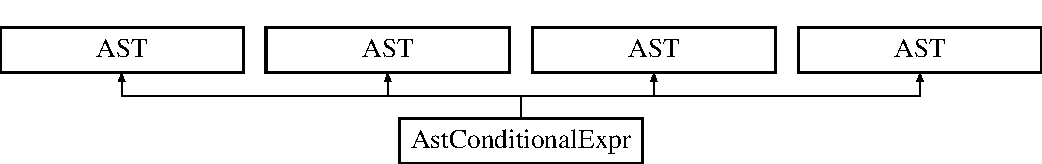
\includegraphics[height=2.000000cm]{classAstConditionalExpr}
\end{center}
\end{figure}
\subsection*{Public Member Functions}
\begin{DoxyCompactItemize}
\item 
\hypertarget{classAstConditionalExpr_a4adcfd01b6eb5f4fb693e085a27953ee}{{\bfseries Ast\-Conditional\-Expr} (\hyperlink{classAstLogicOrExpr}{Ast\-Logic\-Or\-Expr} $\ast$o)}\label{classAstConditionalExpr_a4adcfd01b6eb5f4fb693e085a27953ee}

\item 
\hypertarget{classAstConditionalExpr_aa65a02af9e4ccd958607efcdabdc195f}{{\bfseries Ast\-Conditional\-Expr} (\hyperlink{classAstLogicOrExpr}{Ast\-Logic\-Or\-Expr} $\ast$o, \hyperlink{classAstExpression}{Ast\-Expression} $\ast$e, \hyperlink{classAstConditionalExpr}{Ast\-Conditional\-Expr} $\ast$ce)}\label{classAstConditionalExpr_aa65a02af9e4ccd958607efcdabdc195f}

\item 
void \hyperlink{classAstConditionalExpr_af62c2b118fd6064ec838435ffa72f48c}{Visit} ()
\begin{DoxyCompactList}\small\item\em This function is responsible for tree traversals. \end{DoxyCompactList}\item 
void \hyperlink{classAST_a71d680856e95ff89f55d5311a552eba6}{set\-Label} (string l)
\begin{DoxyCompactList}\small\item\em Sets the label for the node. \end{DoxyCompactList}\item 
int \hyperlink{classAST_ab7a5b1d9f1c2de0d98deb356f724a42c}{get\-U\-I\-D} ()
\begin{DoxyCompactList}\small\item\em Gets the node's unique I\-D. \end{DoxyCompactList}\item 
string \hyperlink{classAST_aee029be902fffc927d16ccb03eb922ad}{get\-Label} ()
\begin{DoxyCompactList}\small\item\em Gets the node's label. \end{DoxyCompactList}\end{DoxyCompactItemize}
\subsection*{Static Public Attributes}
\begin{DoxyCompactItemize}
\item 
\hypertarget{classAST_aca9e6637209b31e03a09c0d42f29bdfa}{static \hyperlink{classVisualizer}{Visualizer} \hyperlink{classAST_aca9e6637209b31e03a09c0d42f29bdfa}{vis}}\label{classAST_aca9e6637209b31e03a09c0d42f29bdfa}

\begin{DoxyCompactList}\small\item\em Static visualizer instance for generating the visualization of the \hyperlink{classAST}{A\-S\-T}. \end{DoxyCompactList}\end{DoxyCompactItemize}
\subsection*{Protected Attributes}
\begin{DoxyCompactItemize}
\item 
\hypertarget{classAST_a847b778f1c3dd5a19de32de432ee6e15}{int \hyperlink{classAST_a847b778f1c3dd5a19de32de432ee6e15}{uid}}\label{classAST_a847b778f1c3dd5a19de32de432ee6e15}

\begin{DoxyCompactList}\small\item\em The unique id. \end{DoxyCompactList}\item 
\hypertarget{classAST_ab2e239ccc0688d2341724432ff5a1a31}{string \hyperlink{classAST_ab2e239ccc0688d2341724432ff5a1a31}{label}}\label{classAST_ab2e239ccc0688d2341724432ff5a1a31}

\begin{DoxyCompactList}\small\item\em The label to be printed in the visualization. \end{DoxyCompactList}\end{DoxyCompactItemize}
\subsection*{Private Attributes}
\begin{DoxyCompactItemize}
\item 
\hypertarget{classAstConditionalExpr_afb5c95122ed18e359b4ab67d65c614b1}{\hyperlink{classAstLogicOrExpr}{Ast\-Logic\-Or\-Expr} $\ast$ {\bfseries o}}\label{classAstConditionalExpr_afb5c95122ed18e359b4ab67d65c614b1}

\item 
\hypertarget{classAstConditionalExpr_ac0dc3162f2834170fc10c6904a2d93d1}{\hyperlink{classAstExpression}{Ast\-Expression} $\ast$ {\bfseries e}}\label{classAstConditionalExpr_ac0dc3162f2834170fc10c6904a2d93d1}

\item 
\hypertarget{classAstConditionalExpr_a69c070ce68c209f09cc5876945c743e7}{\hyperlink{classAstConditionalExpr}{Ast\-Conditional\-Expr} $\ast$ {\bfseries ce}}\label{classAstConditionalExpr_a69c070ce68c209f09cc5876945c743e7}

\end{DoxyCompactItemize}


\subsection{Member Function Documentation}
\hypertarget{classAST_aee029be902fffc927d16ccb03eb922ad}{\index{Ast\-Conditional\-Expr@{Ast\-Conditional\-Expr}!get\-Label@{get\-Label}}
\index{get\-Label@{get\-Label}!AstConditionalExpr@{Ast\-Conditional\-Expr}}
\subsubsection[{get\-Label}]{\setlength{\rightskip}{0pt plus 5cm}string A\-S\-T\-::get\-Label (
\begin{DoxyParamCaption}
{}
\end{DoxyParamCaption}
)\hspace{0.3cm}{\ttfamily [inline]}, {\ttfamily [inherited]}}}\label{classAST_aee029be902fffc927d16ccb03eb922ad}


Gets the node's label. 

\begin{DoxyReturn}{Returns}
The label 
\end{DoxyReturn}
\hypertarget{classAST_ab7a5b1d9f1c2de0d98deb356f724a42c}{\index{Ast\-Conditional\-Expr@{Ast\-Conditional\-Expr}!get\-U\-I\-D@{get\-U\-I\-D}}
\index{get\-U\-I\-D@{get\-U\-I\-D}!AstConditionalExpr@{Ast\-Conditional\-Expr}}
\subsubsection[{get\-U\-I\-D}]{\setlength{\rightskip}{0pt plus 5cm}int A\-S\-T\-::get\-U\-I\-D (
\begin{DoxyParamCaption}
{}
\end{DoxyParamCaption}
)\hspace{0.3cm}{\ttfamily [inline]}, {\ttfamily [inherited]}}}\label{classAST_ab7a5b1d9f1c2de0d98deb356f724a42c}


Gets the node's unique I\-D. 

\begin{DoxyReturn}{Returns}
The unique id 
\end{DoxyReturn}
\hypertarget{classAST_a71d680856e95ff89f55d5311a552eba6}{\index{Ast\-Conditional\-Expr@{Ast\-Conditional\-Expr}!set\-Label@{set\-Label}}
\index{set\-Label@{set\-Label}!AstConditionalExpr@{Ast\-Conditional\-Expr}}
\subsubsection[{set\-Label}]{\setlength{\rightskip}{0pt plus 5cm}void A\-S\-T\-::set\-Label (
\begin{DoxyParamCaption}
\item[{string}]{l}
\end{DoxyParamCaption}
)\hspace{0.3cm}{\ttfamily [inline]}, {\ttfamily [inherited]}}}\label{classAST_a71d680856e95ff89f55d5311a552eba6}


Sets the label for the node. 


\begin{DoxyParams}{Parameters}
{\em l} & The label string \\
\hline
\end{DoxyParams}
\hypertarget{classAstConditionalExpr_af62c2b118fd6064ec838435ffa72f48c}{\index{Ast\-Conditional\-Expr@{Ast\-Conditional\-Expr}!Visit@{Visit}}
\index{Visit@{Visit}!AstConditionalExpr@{Ast\-Conditional\-Expr}}
\subsubsection[{Visit}]{\setlength{\rightskip}{0pt plus 5cm}void Ast\-Conditional\-Expr\-::\-Visit (
\begin{DoxyParamCaption}
{}
\end{DoxyParamCaption}
)\hspace{0.3cm}{\ttfamily [virtual]}}}\label{classAstConditionalExpr_af62c2b118fd6064ec838435ffa72f48c}


This function is responsible for tree traversals. 

This function will call the Visit functions of each of it's children nodes, call the visualization code for itself, and output any 3\-A\-C that can be generated at the current node. 

Reimplemented from \hyperlink{classAST_a5828cc86f2c4f1a0aeab6d7069e8fd82}{A\-S\-T}.



The documentation for this class was generated from the following files\-:\begin{DoxyCompactItemize}
\item 
Ast.\-h\item 
Ast.\-cpp\end{DoxyCompactItemize}

\hypertarget{classAstConstant}{\section{Ast\-Constant Class Reference}
\label{classAstConstant}\index{Ast\-Constant@{Ast\-Constant}}
}
Inheritance diagram for Ast\-Constant\-:\begin{figure}[H]
\begin{center}
\leavevmode
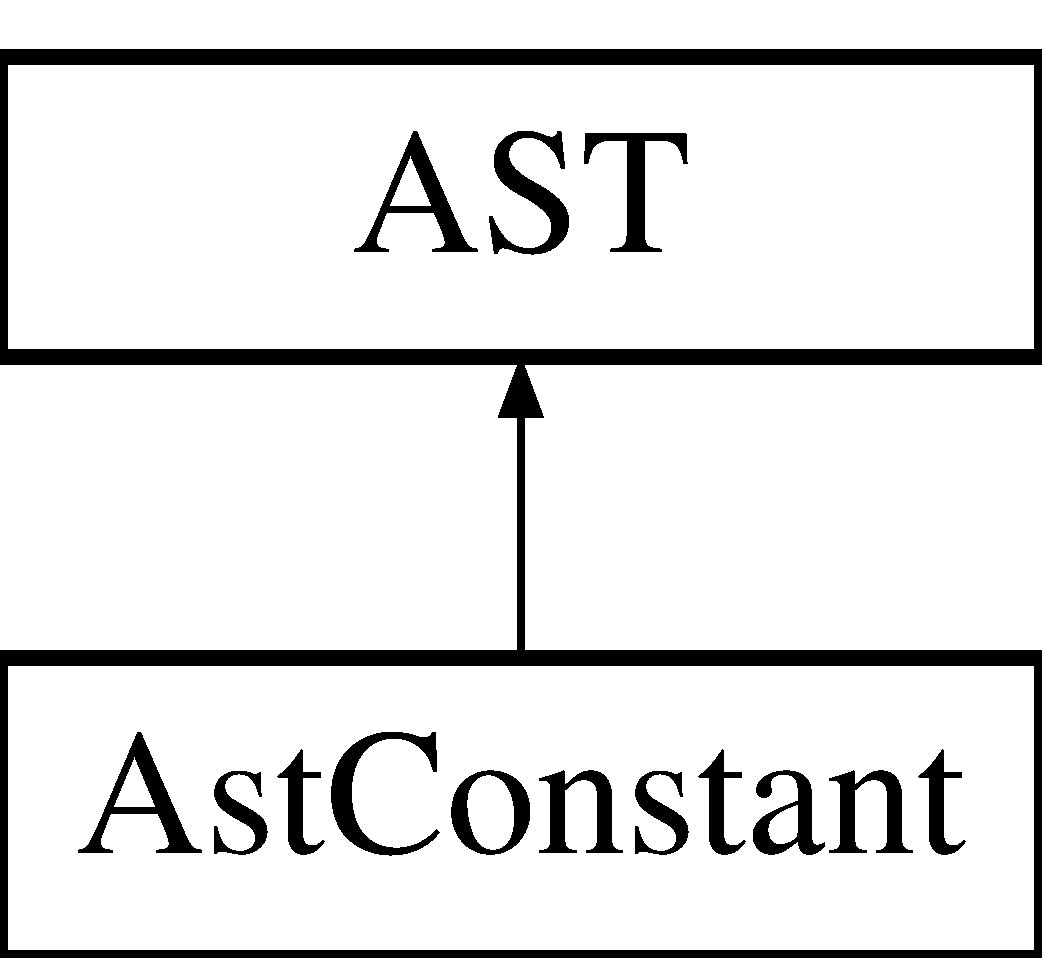
\includegraphics[height=2.000000cm]{classAstConstant}
\end{center}
\end{figure}
\subsection*{Public Types}
\begin{DoxyCompactItemize}
\item 
enum {\bfseries Const\-Type} \{ \\*
{\bfseries I\-N\-T}, 
{\bfseries C\-H\-A\-R}, 
{\bfseries F\-L\-O\-A\-T}, 
{\bfseries E\-N\-U\-M}, 
\\*
{\bfseries I\-N\-T}, 
{\bfseries C\-H\-A\-R}, 
{\bfseries F\-L\-O\-A\-T}, 
{\bfseries E\-N\-U\-M}, 
\\*
{\bfseries I\-N\-T}, 
{\bfseries C\-H\-A\-R}, 
{\bfseries F\-L\-O\-A\-T}, 
{\bfseries E\-N\-U\-M}, 
\\*
{\bfseries I\-N\-T}, 
{\bfseries C\-H\-A\-R}, 
{\bfseries F\-L\-O\-A\-T}, 
{\bfseries E\-N\-U\-M}
 \}
\item 
enum {\bfseries Const\-Type} \{ \\*
{\bfseries I\-N\-T}, 
{\bfseries C\-H\-A\-R}, 
{\bfseries F\-L\-O\-A\-T}, 
{\bfseries E\-N\-U\-M}, 
\\*
{\bfseries I\-N\-T}, 
{\bfseries C\-H\-A\-R}, 
{\bfseries F\-L\-O\-A\-T}, 
{\bfseries E\-N\-U\-M}, 
\\*
{\bfseries I\-N\-T}, 
{\bfseries C\-H\-A\-R}, 
{\bfseries F\-L\-O\-A\-T}, 
{\bfseries E\-N\-U\-M}, 
\\*
{\bfseries I\-N\-T}, 
{\bfseries C\-H\-A\-R}, 
{\bfseries F\-L\-O\-A\-T}, 
{\bfseries E\-N\-U\-M}
 \}
\item 
enum {\bfseries Const\-Type} \{ \\*
{\bfseries I\-N\-T}, 
{\bfseries C\-H\-A\-R}, 
{\bfseries F\-L\-O\-A\-T}, 
{\bfseries E\-N\-U\-M}, 
\\*
{\bfseries I\-N\-T}, 
{\bfseries C\-H\-A\-R}, 
{\bfseries F\-L\-O\-A\-T}, 
{\bfseries E\-N\-U\-M}, 
\\*
{\bfseries I\-N\-T}, 
{\bfseries C\-H\-A\-R}, 
{\bfseries F\-L\-O\-A\-T}, 
{\bfseries E\-N\-U\-M}, 
\\*
{\bfseries I\-N\-T}, 
{\bfseries C\-H\-A\-R}, 
{\bfseries F\-L\-O\-A\-T}, 
{\bfseries E\-N\-U\-M}
 \}
\item 
enum {\bfseries Const\-Type} \{ \\*
{\bfseries I\-N\-T}, 
{\bfseries C\-H\-A\-R}, 
{\bfseries F\-L\-O\-A\-T}, 
{\bfseries E\-N\-U\-M}, 
\\*
{\bfseries I\-N\-T}, 
{\bfseries C\-H\-A\-R}, 
{\bfseries F\-L\-O\-A\-T}, 
{\bfseries E\-N\-U\-M}, 
\\*
{\bfseries I\-N\-T}, 
{\bfseries C\-H\-A\-R}, 
{\bfseries F\-L\-O\-A\-T}, 
{\bfseries E\-N\-U\-M}, 
\\*
{\bfseries I\-N\-T}, 
{\bfseries C\-H\-A\-R}, 
{\bfseries F\-L\-O\-A\-T}, 
{\bfseries E\-N\-U\-M}
 \}
\end{DoxyCompactItemize}
\subsection*{Public Member Functions}
\begin{DoxyCompactItemize}
\item 
\hypertarget{classAstConstant_ab3d7bb141b6d2650498569fa7742237f}{{\bfseries Ast\-Constant} (int val)}\label{classAstConstant_ab3d7bb141b6d2650498569fa7742237f}

\item 
\hypertarget{classAstConstant_a071adbaa9ea9ad30cde38d68b4182cd9}{{\bfseries Ast\-Constant} (string val)}\label{classAstConstant_a071adbaa9ea9ad30cde38d68b4182cd9}

\item 
\hypertarget{classAstConstant_aef9142c2750c7ad8e83183c7b8ade0e8}{{\bfseries Ast\-Constant} (double val)}\label{classAstConstant_aef9142c2750c7ad8e83183c7b8ade0e8}

\item 
\hypertarget{classAstConstant_a9ceaff3b1de813268a88d7fded0aeb0c}{{\bfseries Ast\-Constant} (int val, string name, \hyperlink{classType}{Type} $\ast$t)}\label{classAstConstant_a9ceaff3b1de813268a88d7fded0aeb0c}

\item 
void \hyperlink{classAstConstant_ac13b7246f9d646a5ff00efee4c39bc6b}{Visit} ()
\begin{DoxyCompactList}\small\item\em This function is responsible for tree traversals. \end{DoxyCompactList}\item 
\hypertarget{classAstConstant_ab3d7bb141b6d2650498569fa7742237f}{{\bfseries Ast\-Constant} (int val)}\label{classAstConstant_ab3d7bb141b6d2650498569fa7742237f}

\item 
\hypertarget{classAstConstant_a071adbaa9ea9ad30cde38d68b4182cd9}{{\bfseries Ast\-Constant} (string val)}\label{classAstConstant_a071adbaa9ea9ad30cde38d68b4182cd9}

\item 
\hypertarget{classAstConstant_aef9142c2750c7ad8e83183c7b8ade0e8}{{\bfseries Ast\-Constant} (double val)}\label{classAstConstant_aef9142c2750c7ad8e83183c7b8ade0e8}

\item 
\hypertarget{classAstConstant_a9ceaff3b1de813268a88d7fded0aeb0c}{{\bfseries Ast\-Constant} (int val, string name, \hyperlink{classType}{Type} $\ast$t)}\label{classAstConstant_a9ceaff3b1de813268a88d7fded0aeb0c}

\item 
void \hyperlink{classAstConstant_ac13b7246f9d646a5ff00efee4c39bc6b}{Visit} ()
\begin{DoxyCompactList}\small\item\em This function is responsible for tree traversals. \end{DoxyCompactList}\item 
\hypertarget{classAstConstant_ab3d7bb141b6d2650498569fa7742237f}{{\bfseries Ast\-Constant} (int val)}\label{classAstConstant_ab3d7bb141b6d2650498569fa7742237f}

\item 
\hypertarget{classAstConstant_a071adbaa9ea9ad30cde38d68b4182cd9}{{\bfseries Ast\-Constant} (string val)}\label{classAstConstant_a071adbaa9ea9ad30cde38d68b4182cd9}

\item 
\hypertarget{classAstConstant_aef9142c2750c7ad8e83183c7b8ade0e8}{{\bfseries Ast\-Constant} (double val)}\label{classAstConstant_aef9142c2750c7ad8e83183c7b8ade0e8}

\item 
\hypertarget{classAstConstant_a9ceaff3b1de813268a88d7fded0aeb0c}{{\bfseries Ast\-Constant} (int val, string name, \hyperlink{classType}{Type} $\ast$t)}\label{classAstConstant_a9ceaff3b1de813268a88d7fded0aeb0c}

\item 
void \hyperlink{classAstConstant_ac13b7246f9d646a5ff00efee4c39bc6b}{Visit} ()
\begin{DoxyCompactList}\small\item\em This function is responsible for tree traversals. \end{DoxyCompactList}\item 
\hypertarget{classAstConstant_ab3d7bb141b6d2650498569fa7742237f}{{\bfseries Ast\-Constant} (int val)}\label{classAstConstant_ab3d7bb141b6d2650498569fa7742237f}

\item 
\hypertarget{classAstConstant_a071adbaa9ea9ad30cde38d68b4182cd9}{{\bfseries Ast\-Constant} (string val)}\label{classAstConstant_a071adbaa9ea9ad30cde38d68b4182cd9}

\item 
\hypertarget{classAstConstant_aef9142c2750c7ad8e83183c7b8ade0e8}{{\bfseries Ast\-Constant} (double val)}\label{classAstConstant_aef9142c2750c7ad8e83183c7b8ade0e8}

\item 
\hypertarget{classAstConstant_a9ceaff3b1de813268a88d7fded0aeb0c}{{\bfseries Ast\-Constant} (int val, string name, \hyperlink{classType}{Type} $\ast$t)}\label{classAstConstant_a9ceaff3b1de813268a88d7fded0aeb0c}

\item 
void \hyperlink{classAstConstant_ac13b7246f9d646a5ff00efee4c39bc6b}{Visit} ()
\begin{DoxyCompactList}\small\item\em This function is responsible for tree traversals. \end{DoxyCompactList}\item 
void \hyperlink{classAST_a71d680856e95ff89f55d5311a552eba6}{set\-Label} (string l)
\begin{DoxyCompactList}\small\item\em Sets the label for the node. \end{DoxyCompactList}\item 
void \hyperlink{classAST_a71d680856e95ff89f55d5311a552eba6}{set\-Label} (string l)
\begin{DoxyCompactList}\small\item\em Sets the label for the node. \end{DoxyCompactList}\item 
void \hyperlink{classAST_a71d680856e95ff89f55d5311a552eba6}{set\-Label} (string l)
\begin{DoxyCompactList}\small\item\em Sets the label for the node. \end{DoxyCompactList}\item 
void \hyperlink{classAST_a71d680856e95ff89f55d5311a552eba6}{set\-Label} (string l)
\begin{DoxyCompactList}\small\item\em Sets the label for the node. \end{DoxyCompactList}\item 
int \hyperlink{classAST_ab7a5b1d9f1c2de0d98deb356f724a42c}{get\-U\-I\-D} ()
\begin{DoxyCompactList}\small\item\em Gets the node's unique I\-D. \end{DoxyCompactList}\item 
int \hyperlink{classAST_ab7a5b1d9f1c2de0d98deb356f724a42c}{get\-U\-I\-D} ()
\begin{DoxyCompactList}\small\item\em Gets the node's unique I\-D. \end{DoxyCompactList}\item 
int \hyperlink{classAST_ab7a5b1d9f1c2de0d98deb356f724a42c}{get\-U\-I\-D} ()
\begin{DoxyCompactList}\small\item\em Gets the node's unique I\-D. \end{DoxyCompactList}\item 
int \hyperlink{classAST_ab7a5b1d9f1c2de0d98deb356f724a42c}{get\-U\-I\-D} ()
\begin{DoxyCompactList}\small\item\em Gets the node's unique I\-D. \end{DoxyCompactList}\item 
string \hyperlink{classAST_aee029be902fffc927d16ccb03eb922ad}{get\-Label} ()
\begin{DoxyCompactList}\small\item\em Gets the node's label. \end{DoxyCompactList}\item 
string \hyperlink{classAST_aee029be902fffc927d16ccb03eb922ad}{get\-Label} ()
\begin{DoxyCompactList}\small\item\em Gets the node's label. \end{DoxyCompactList}\item 
string \hyperlink{classAST_aee029be902fffc927d16ccb03eb922ad}{get\-Label} ()
\begin{DoxyCompactList}\small\item\em Gets the node's label. \end{DoxyCompactList}\item 
string \hyperlink{classAST_aee029be902fffc927d16ccb03eb922ad}{get\-Label} ()
\begin{DoxyCompactList}\small\item\em Gets the node's label. \end{DoxyCompactList}\end{DoxyCompactItemize}
\subsection*{Public Attributes}
\begin{DoxyCompactItemize}
\item 
\hypertarget{classAstConstant_ad350f1bd35d56369731660f8f8c826e7}{Const\-Type {\bfseries type}}\label{classAstConstant_ad350f1bd35d56369731660f8f8c826e7}

\item 
\hypertarget{classAstConstant_a45b3874ec43dac2b0b56fca2f70ae310}{int {\bfseries ival}}\label{classAstConstant_a45b3874ec43dac2b0b56fca2f70ae310}

\item 
\hypertarget{classAstConstant_a79f98612fb8aa367b279ad199c794b31}{string {\bfseries str}}\label{classAstConstant_a79f98612fb8aa367b279ad199c794b31}

\item 
\hypertarget{classAstConstant_a6a7521fd6217f7d8eba703ba6877be9d}{double {\bfseries dval}}\label{classAstConstant_a6a7521fd6217f7d8eba703ba6877be9d}

\item 
\hypertarget{classAstConstant_a509ff0f489033b055f21b984dcb96b8f}{\hyperlink{classType}{Type} $\ast$ {\bfseries etype}}\label{classAstConstant_a509ff0f489033b055f21b984dcb96b8f}

\item 
\hypertarget{classAST_aaf215802de409f8096c063d01ffa6783}{bool \hyperlink{classAST_aaf215802de409f8096c063d01ffa6783}{needs\-Cast}}\label{classAST_aaf215802de409f8096c063d01ffa6783}

\begin{DoxyCompactList}\small\item\em This indicates if cast 3\-A\-C needs to be output, and is only relevant for expressions. \end{DoxyCompactList}\item 
\hypertarget{classAST_afa9e77ef650ec6664458fa6cb55be985}{bool \hyperlink{classAST_afa9e77ef650ec6664458fa6cb55be985}{is\-Conv}}\label{classAST_afa9e77ef650ec6664458fa6cb55be985}

\begin{DoxyCompactList}\small\item\em Indicates is a conversion is possible. \end{DoxyCompactList}\item 
\hypertarget{classAST_a61ef3317e023d45237e06615b387cd6b}{C\-O\-N\-V\-E\-R\-S\-I\-O\-N\-T\-Y\-P\-E \hyperlink{classAST_a61ef3317e023d45237e06615b387cd6b}{conv\-Type}}\label{classAST_a61ef3317e023d45237e06615b387cd6b}

\begin{DoxyCompactList}\small\item\em If needs\-Cast is true, then this indicates what the cast should be. \end{DoxyCompactList}\item 
\hypertarget{classAST_aea9b07b39d24183f38c0029cec0a878e}{int \hyperlink{classAST_aea9b07b39d24183f38c0029cec0a878e}{operand\-To\-Cast}}\label{classAST_aea9b07b39d24183f38c0029cec0a878e}

\begin{DoxyCompactList}\small\item\em This indicates if the first or second operand should be the one that is cast. \end{DoxyCompactList}\end{DoxyCompactItemize}
\subsection*{Static Public Attributes}
\begin{DoxyCompactItemize}
\item 
\hypertarget{classAST_a5fdfd5f7b104dd92889163bdadbc68d6}{static \hyperlink{classVisualizer}{Visualizer} \hyperlink{classAST_a5fdfd5f7b104dd92889163bdadbc68d6}{vis}}\label{classAST_a5fdfd5f7b104dd92889163bdadbc68d6}

\begin{DoxyCompactList}\small\item\em Static visualizer instance for generating the visualization of the \hyperlink{classAST}{A\-S\-T}. \end{DoxyCompactList}\item 
\hypertarget{classAST_a8a3ace322f50e030331065d644ee55ee}{static \hyperlink{classTAC__Generator}{T\-A\-C\-\_\-\-Generator} \hyperlink{classAST_a8a3ace322f50e030331065d644ee55ee}{tac\-Gen}}\label{classAST_a8a3ace322f50e030331065d644ee55ee}

\begin{DoxyCompactList}\small\item\em Three address code generator. \end{DoxyCompactList}\item 
\hypertarget{classAST_a1f69448c6dc368d005631a128460083d}{static string {\bfseries current\-Temp} =\char`\"{}\char`\"{}}\label{classAST_a1f69448c6dc368d005631a128460083d}

\item 
\hypertarget{classAST_a551aec090c932ab69365238b40a8a4eb}{static string \hyperlink{classAST_a551aec090c932ab69365238b40a8a4eb}{return\-Label} =\char`\"{}\char`\"{}}\label{classAST_a551aec090c932ab69365238b40a8a4eb}

\begin{DoxyCompactList}\small\item\em This is for storing the string id of any temporary result register that may be created during 3\-A\-C generation. \end{DoxyCompactList}\item 
\hypertarget{classAST_a73c0a266df52be71e6b527b6aa635173}{static list$<$ string $>$ {\bfseries temp\-Stack}}\label{classAST_a73c0a266df52be71e6b527b6aa635173}

\item 
\hypertarget{classAST_abf9e84b541ff04b7bb64e6e4371512d4}{static string {\bfseries last\-I\-D} =\char`\"{}\char`\"{}}\label{classAST_abf9e84b541ff04b7bb64e6e4371512d4}

\item 
\hypertarget{classAST_a163003bfe9c30510ec8039870346049f}{static \hyperlink{classSymTab}{Sym\-Tab} $\ast$ {\bfseries symbol\-Table} =N\-U\-L\-L}\label{classAST_a163003bfe9c30510ec8039870346049f}

\item 
\hypertarget{classAST_a5c3cc894d9c0453523dec9ed76f18a04}{static string {\bfseries current\-Function} =\char`\"{}\char`\"{}}\label{classAST_a5c3cc894d9c0453523dec9ed76f18a04}

\item 
\hypertarget{classAST_a66155513b59ff1a04c8ece8b20ec31f5}{static int {\bfseries current\-Constant\-Value} =0}\label{classAST_a66155513b59ff1a04c8ece8b20ec31f5}

\item 
\hypertarget{classAST_a3d031d7bab635ba1f015aade5943f40c}{static string {\bfseries current\-Id\-Name} =\char`\"{}\char`\"{}}\label{classAST_a3d031d7bab635ba1f015aade5943f40c}

\item 
\hypertarget{classAST_a16c4b6e54febc1a26b31a64a46972ef0}{static int {\bfseries current\-Index\-Val} = 0}\label{classAST_a16c4b6e54febc1a26b31a64a46972ef0}

\item 
\hypertarget{classAST_a6fc65ae9dd064a88941d4b88669b19db}{static string {\bfseries current\-I\-D} = \char`\"{}\char`\"{}}\label{classAST_a6fc65ae9dd064a88941d4b88669b19db}

\end{DoxyCompactItemize}
\subsection*{Protected Attributes}
\begin{DoxyCompactItemize}
\item 
\hypertarget{classAST_a847b778f1c3dd5a19de32de432ee6e15}{int \hyperlink{classAST_a847b778f1c3dd5a19de32de432ee6e15}{uid}}\label{classAST_a847b778f1c3dd5a19de32de432ee6e15}

\begin{DoxyCompactList}\small\item\em The unique id. \end{DoxyCompactList}\item 
\hypertarget{classAST_ab2e239ccc0688d2341724432ff5a1a31}{string \hyperlink{classAST_ab2e239ccc0688d2341724432ff5a1a31}{label}}\label{classAST_ab2e239ccc0688d2341724432ff5a1a31}

\begin{DoxyCompactList}\small\item\em The label to be printed in the visualization. \end{DoxyCompactList}\end{DoxyCompactItemize}


\subsection{Detailed Description}


Definition at line 144 of file Ast.\-h.



\subsection{Member Function Documentation}
\hypertarget{classAST_aee029be902fffc927d16ccb03eb922ad}{\index{Ast\-Constant@{Ast\-Constant}!get\-Label@{get\-Label}}
\index{get\-Label@{get\-Label}!AstConstant@{Ast\-Constant}}
\subsubsection[{get\-Label}]{\setlength{\rightskip}{0pt plus 5cm}string A\-S\-T\-::get\-Label (
\begin{DoxyParamCaption}
{}
\end{DoxyParamCaption}
)\hspace{0.3cm}{\ttfamily [inline]}, {\ttfamily [inherited]}}}\label{classAST_aee029be902fffc927d16ccb03eb922ad}


Gets the node's label. 

\begin{DoxyReturn}{Returns}
The label 
\end{DoxyReturn}


Definition at line 60 of file Ast.\-h.

\hypertarget{classAST_aee029be902fffc927d16ccb03eb922ad}{\index{Ast\-Constant@{Ast\-Constant}!get\-Label@{get\-Label}}
\index{get\-Label@{get\-Label}!AstConstant@{Ast\-Constant}}
\subsubsection[{get\-Label}]{\setlength{\rightskip}{0pt plus 5cm}string A\-S\-T\-::get\-Label (
\begin{DoxyParamCaption}
{}
\end{DoxyParamCaption}
)\hspace{0.3cm}{\ttfamily [inline]}, {\ttfamily [inherited]}}}\label{classAST_aee029be902fffc927d16ccb03eb922ad}


Gets the node's label. 

\begin{DoxyReturn}{Returns}
The label 
\end{DoxyReturn}


Definition at line 60 of file C\-Scanner.\-ll.

\hypertarget{classAST_aee029be902fffc927d16ccb03eb922ad}{\index{Ast\-Constant@{Ast\-Constant}!get\-Label@{get\-Label}}
\index{get\-Label@{get\-Label}!AstConstant@{Ast\-Constant}}
\subsubsection[{get\-Label}]{\setlength{\rightskip}{0pt plus 5cm}string A\-S\-T\-::get\-Label (
\begin{DoxyParamCaption}
{}
\end{DoxyParamCaption}
)\hspace{0.3cm}{\ttfamily [inline]}, {\ttfamily [inherited]}}}\label{classAST_aee029be902fffc927d16ccb03eb922ad}


Gets the node's label. 

\begin{DoxyReturn}{Returns}
The label 
\end{DoxyReturn}


Definition at line 60 of file C\-Parser.\-yy.

\hypertarget{classAST_aee029be902fffc927d16ccb03eb922ad}{\index{Ast\-Constant@{Ast\-Constant}!get\-Label@{get\-Label}}
\index{get\-Label@{get\-Label}!AstConstant@{Ast\-Constant}}
\subsubsection[{get\-Label}]{\setlength{\rightskip}{0pt plus 5cm}string A\-S\-T\-::get\-Label (
\begin{DoxyParamCaption}
{}
\end{DoxyParamCaption}
)\hspace{0.3cm}{\ttfamily [inline]}, {\ttfamily [inherited]}}}\label{classAST_aee029be902fffc927d16ccb03eb922ad}


Gets the node's label. 

\begin{DoxyReturn}{Returns}
The label 
\end{DoxyReturn}


Definition at line 60 of file C\-Parser.\-yy.

\hypertarget{classAST_ab7a5b1d9f1c2de0d98deb356f724a42c}{\index{Ast\-Constant@{Ast\-Constant}!get\-U\-I\-D@{get\-U\-I\-D}}
\index{get\-U\-I\-D@{get\-U\-I\-D}!AstConstant@{Ast\-Constant}}
\subsubsection[{get\-U\-I\-D}]{\setlength{\rightskip}{0pt plus 5cm}int A\-S\-T\-::get\-U\-I\-D (
\begin{DoxyParamCaption}
{}
\end{DoxyParamCaption}
)\hspace{0.3cm}{\ttfamily [inline]}, {\ttfamily [inherited]}}}\label{classAST_ab7a5b1d9f1c2de0d98deb356f724a42c}


Gets the node's unique I\-D. 

\begin{DoxyReturn}{Returns}
The unique id 
\end{DoxyReturn}


Definition at line 53 of file C\-Parser.\-yy.

\hypertarget{classAST_ab7a5b1d9f1c2de0d98deb356f724a42c}{\index{Ast\-Constant@{Ast\-Constant}!get\-U\-I\-D@{get\-U\-I\-D}}
\index{get\-U\-I\-D@{get\-U\-I\-D}!AstConstant@{Ast\-Constant}}
\subsubsection[{get\-U\-I\-D}]{\setlength{\rightskip}{0pt plus 5cm}int A\-S\-T\-::get\-U\-I\-D (
\begin{DoxyParamCaption}
{}
\end{DoxyParamCaption}
)\hspace{0.3cm}{\ttfamily [inline]}, {\ttfamily [inherited]}}}\label{classAST_ab7a5b1d9f1c2de0d98deb356f724a42c}


Gets the node's unique I\-D. 

\begin{DoxyReturn}{Returns}
The unique id 
\end{DoxyReturn}


Definition at line 53 of file C\-Parser.\-yy.

\hypertarget{classAST_ab7a5b1d9f1c2de0d98deb356f724a42c}{\index{Ast\-Constant@{Ast\-Constant}!get\-U\-I\-D@{get\-U\-I\-D}}
\index{get\-U\-I\-D@{get\-U\-I\-D}!AstConstant@{Ast\-Constant}}
\subsubsection[{get\-U\-I\-D}]{\setlength{\rightskip}{0pt plus 5cm}int A\-S\-T\-::get\-U\-I\-D (
\begin{DoxyParamCaption}
{}
\end{DoxyParamCaption}
)\hspace{0.3cm}{\ttfamily [inline]}, {\ttfamily [inherited]}}}\label{classAST_ab7a5b1d9f1c2de0d98deb356f724a42c}


Gets the node's unique I\-D. 

\begin{DoxyReturn}{Returns}
The unique id 
\end{DoxyReturn}


Definition at line 53 of file C\-Scanner.\-ll.

\hypertarget{classAST_ab7a5b1d9f1c2de0d98deb356f724a42c}{\index{Ast\-Constant@{Ast\-Constant}!get\-U\-I\-D@{get\-U\-I\-D}}
\index{get\-U\-I\-D@{get\-U\-I\-D}!AstConstant@{Ast\-Constant}}
\subsubsection[{get\-U\-I\-D}]{\setlength{\rightskip}{0pt plus 5cm}int A\-S\-T\-::get\-U\-I\-D (
\begin{DoxyParamCaption}
{}
\end{DoxyParamCaption}
)\hspace{0.3cm}{\ttfamily [inline]}, {\ttfamily [inherited]}}}\label{classAST_ab7a5b1d9f1c2de0d98deb356f724a42c}


Gets the node's unique I\-D. 

\begin{DoxyReturn}{Returns}
The unique id 
\end{DoxyReturn}


Definition at line 53 of file Ast.\-h.

\hypertarget{classAST_a71d680856e95ff89f55d5311a552eba6}{\index{Ast\-Constant@{Ast\-Constant}!set\-Label@{set\-Label}}
\index{set\-Label@{set\-Label}!AstConstant@{Ast\-Constant}}
\subsubsection[{set\-Label}]{\setlength{\rightskip}{0pt plus 5cm}void A\-S\-T\-::set\-Label (
\begin{DoxyParamCaption}
\item[{string}]{l}
\end{DoxyParamCaption}
)\hspace{0.3cm}{\ttfamily [inline]}, {\ttfamily [inherited]}}}\label{classAST_a71d680856e95ff89f55d5311a552eba6}


Sets the label for the node. 


\begin{DoxyParams}{Parameters}
{\em l} & The label string \\
\hline
\end{DoxyParams}


Definition at line 43 of file C\-Scanner.\-ll.

\hypertarget{classAST_a71d680856e95ff89f55d5311a552eba6}{\index{Ast\-Constant@{Ast\-Constant}!set\-Label@{set\-Label}}
\index{set\-Label@{set\-Label}!AstConstant@{Ast\-Constant}}
\subsubsection[{set\-Label}]{\setlength{\rightskip}{0pt plus 5cm}void A\-S\-T\-::set\-Label (
\begin{DoxyParamCaption}
\item[{string}]{l}
\end{DoxyParamCaption}
)\hspace{0.3cm}{\ttfamily [inline]}, {\ttfamily [inherited]}}}\label{classAST_a71d680856e95ff89f55d5311a552eba6}


Sets the label for the node. 


\begin{DoxyParams}{Parameters}
{\em l} & The label string \\
\hline
\end{DoxyParams}


Definition at line 43 of file C\-Parser.\-yy.

\hypertarget{classAST_a71d680856e95ff89f55d5311a552eba6}{\index{Ast\-Constant@{Ast\-Constant}!set\-Label@{set\-Label}}
\index{set\-Label@{set\-Label}!AstConstant@{Ast\-Constant}}
\subsubsection[{set\-Label}]{\setlength{\rightskip}{0pt plus 5cm}void A\-S\-T\-::set\-Label (
\begin{DoxyParamCaption}
\item[{string}]{l}
\end{DoxyParamCaption}
)\hspace{0.3cm}{\ttfamily [inline]}, {\ttfamily [inherited]}}}\label{classAST_a71d680856e95ff89f55d5311a552eba6}


Sets the label for the node. 


\begin{DoxyParams}{Parameters}
{\em l} & The label string \\
\hline
\end{DoxyParams}


Definition at line 43 of file Ast.\-h.

\hypertarget{classAST_a71d680856e95ff89f55d5311a552eba6}{\index{Ast\-Constant@{Ast\-Constant}!set\-Label@{set\-Label}}
\index{set\-Label@{set\-Label}!AstConstant@{Ast\-Constant}}
\subsubsection[{set\-Label}]{\setlength{\rightskip}{0pt plus 5cm}void A\-S\-T\-::set\-Label (
\begin{DoxyParamCaption}
\item[{string}]{l}
\end{DoxyParamCaption}
)\hspace{0.3cm}{\ttfamily [inline]}, {\ttfamily [inherited]}}}\label{classAST_a71d680856e95ff89f55d5311a552eba6}


Sets the label for the node. 


\begin{DoxyParams}{Parameters}
{\em l} & The label string \\
\hline
\end{DoxyParams}


Definition at line 43 of file C\-Parser.\-yy.

\hypertarget{classAstConstant_ac13b7246f9d646a5ff00efee4c39bc6b}{\index{Ast\-Constant@{Ast\-Constant}!Visit@{Visit}}
\index{Visit@{Visit}!AstConstant@{Ast\-Constant}}
\subsubsection[{Visit}]{\setlength{\rightskip}{0pt plus 5cm}void Ast\-Constant\-::\-Visit (
\begin{DoxyParamCaption}
{}
\end{DoxyParamCaption}
)\hspace{0.3cm}{\ttfamily [virtual]}}}\label{classAstConstant_ac13b7246f9d646a5ff00efee4c39bc6b}


This function is responsible for tree traversals. 

This function will call the Visit functions of each of it's children nodes, call the visualization code for itself, and output any 3\-A\-C that can be generated at the current node. 

Reimplemented from \hyperlink{classAST_a5828cc86f2c4f1a0aeab6d7069e8fd82}{A\-S\-T}.



Definition at line 925 of file Ast.\-cpp.

\hypertarget{classAstConstant_ac13b7246f9d646a5ff00efee4c39bc6b}{\index{Ast\-Constant@{Ast\-Constant}!Visit@{Visit}}
\index{Visit@{Visit}!AstConstant@{Ast\-Constant}}
\subsubsection[{Visit}]{\setlength{\rightskip}{0pt plus 5cm}void Ast\-Constant\-::\-Visit (
\begin{DoxyParamCaption}
{}
\end{DoxyParamCaption}
)\hspace{0.3cm}{\ttfamily [virtual]}}}\label{classAstConstant_ac13b7246f9d646a5ff00efee4c39bc6b}


This function is responsible for tree traversals. 

This function will call the Visit functions of each of it's children nodes, call the visualization code for itself, and output any 3\-A\-C that can be generated at the current node. 

Reimplemented from \hyperlink{classAST_a5828cc86f2c4f1a0aeab6d7069e8fd82}{A\-S\-T}.

\hypertarget{classAstConstant_ac13b7246f9d646a5ff00efee4c39bc6b}{\index{Ast\-Constant@{Ast\-Constant}!Visit@{Visit}}
\index{Visit@{Visit}!AstConstant@{Ast\-Constant}}
\subsubsection[{Visit}]{\setlength{\rightskip}{0pt plus 5cm}void Ast\-Constant\-::\-Visit (
\begin{DoxyParamCaption}
{}
\end{DoxyParamCaption}
)\hspace{0.3cm}{\ttfamily [virtual]}}}\label{classAstConstant_ac13b7246f9d646a5ff00efee4c39bc6b}


This function is responsible for tree traversals. 

This function will call the Visit functions of each of it's children nodes, call the visualization code for itself, and output any 3\-A\-C that can be generated at the current node. 

Reimplemented from \hyperlink{classAST_a5828cc86f2c4f1a0aeab6d7069e8fd82}{A\-S\-T}.

\hypertarget{classAstConstant_ac13b7246f9d646a5ff00efee4c39bc6b}{\index{Ast\-Constant@{Ast\-Constant}!Visit@{Visit}}
\index{Visit@{Visit}!AstConstant@{Ast\-Constant}}
\subsubsection[{Visit}]{\setlength{\rightskip}{0pt plus 5cm}void Ast\-Constant\-::\-Visit (
\begin{DoxyParamCaption}
{}
\end{DoxyParamCaption}
)\hspace{0.3cm}{\ttfamily [virtual]}}}\label{classAstConstant_ac13b7246f9d646a5ff00efee4c39bc6b}


This function is responsible for tree traversals. 

This function will call the Visit functions of each of it's children nodes, call the visualization code for itself, and output any 3\-A\-C that can be generated at the current node. 

Reimplemented from \hyperlink{classAST_a5828cc86f2c4f1a0aeab6d7069e8fd82}{A\-S\-T}.



The documentation for this class was generated from the following files\-:\begin{DoxyCompactItemize}
\item 
Ast.\-h\item 
Ast.\-cpp\end{DoxyCompactItemize}

\hypertarget{classAstConstantExpr}{\section{Ast\-Constant\-Expr Class Reference}
\label{classAstConstantExpr}\index{Ast\-Constant\-Expr@{Ast\-Constant\-Expr}}
}
Inheritance diagram for Ast\-Constant\-Expr\-:\begin{figure}[H]
\begin{center}
\leavevmode
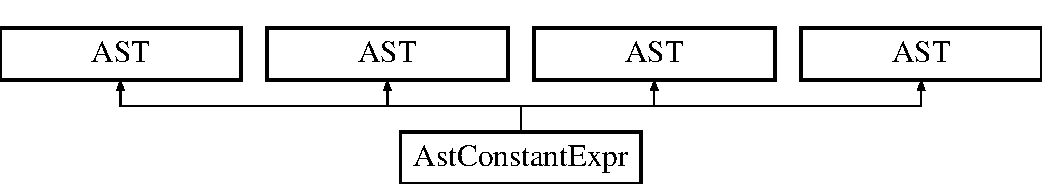
\includegraphics[height=2.000000cm]{classAstConstantExpr}
\end{center}
\end{figure}
\subsection*{Public Member Functions}
\begin{DoxyCompactItemize}
\item 
\hypertarget{classAstConstantExpr_a7a8c30ee91b9addfab3d0df85f9ebc30}{{\bfseries Ast\-Constant\-Expr} (\hyperlink{classAstConditionalExpr}{Ast\-Conditional\-Expr} $\ast$e)}\label{classAstConstantExpr_a7a8c30ee91b9addfab3d0df85f9ebc30}

\item 
void \hyperlink{classAstConstantExpr_a355fbc35bcfa038875468e127527a597}{Visit} ()
\begin{DoxyCompactList}\small\item\em This function is responsible for tree traversals. \end{DoxyCompactList}\item 
\hypertarget{classAstConstantExpr_a7a8c30ee91b9addfab3d0df85f9ebc30}{{\bfseries Ast\-Constant\-Expr} (\hyperlink{classAstConditionalExpr}{Ast\-Conditional\-Expr} $\ast$e)}\label{classAstConstantExpr_a7a8c30ee91b9addfab3d0df85f9ebc30}

\item 
void \hyperlink{classAstConstantExpr_a355fbc35bcfa038875468e127527a597}{Visit} ()
\begin{DoxyCompactList}\small\item\em This function is responsible for tree traversals. \end{DoxyCompactList}\item 
\hypertarget{classAstConstantExpr_a7a8c30ee91b9addfab3d0df85f9ebc30}{{\bfseries Ast\-Constant\-Expr} (\hyperlink{classAstConditionalExpr}{Ast\-Conditional\-Expr} $\ast$e)}\label{classAstConstantExpr_a7a8c30ee91b9addfab3d0df85f9ebc30}

\item 
void \hyperlink{classAstConstantExpr_a355fbc35bcfa038875468e127527a597}{Visit} ()
\begin{DoxyCompactList}\small\item\em This function is responsible for tree traversals. \end{DoxyCompactList}\item 
\hypertarget{classAstConstantExpr_a7a8c30ee91b9addfab3d0df85f9ebc30}{{\bfseries Ast\-Constant\-Expr} (\hyperlink{classAstConditionalExpr}{Ast\-Conditional\-Expr} $\ast$e)}\label{classAstConstantExpr_a7a8c30ee91b9addfab3d0df85f9ebc30}

\item 
void \hyperlink{classAstConstantExpr_a355fbc35bcfa038875468e127527a597}{Visit} ()
\begin{DoxyCompactList}\small\item\em This function is responsible for tree traversals. \end{DoxyCompactList}\item 
void \hyperlink{classAST_a71d680856e95ff89f55d5311a552eba6}{set\-Label} (string l)
\begin{DoxyCompactList}\small\item\em Sets the label for the node. \end{DoxyCompactList}\item 
void \hyperlink{classAST_a71d680856e95ff89f55d5311a552eba6}{set\-Label} (string l)
\begin{DoxyCompactList}\small\item\em Sets the label for the node. \end{DoxyCompactList}\item 
void \hyperlink{classAST_a71d680856e95ff89f55d5311a552eba6}{set\-Label} (string l)
\begin{DoxyCompactList}\small\item\em Sets the label for the node. \end{DoxyCompactList}\item 
void \hyperlink{classAST_a71d680856e95ff89f55d5311a552eba6}{set\-Label} (string l)
\begin{DoxyCompactList}\small\item\em Sets the label for the node. \end{DoxyCompactList}\item 
int \hyperlink{classAST_ab7a5b1d9f1c2de0d98deb356f724a42c}{get\-U\-I\-D} ()
\begin{DoxyCompactList}\small\item\em Gets the node's unique I\-D. \end{DoxyCompactList}\item 
int \hyperlink{classAST_ab7a5b1d9f1c2de0d98deb356f724a42c}{get\-U\-I\-D} ()
\begin{DoxyCompactList}\small\item\em Gets the node's unique I\-D. \end{DoxyCompactList}\item 
int \hyperlink{classAST_ab7a5b1d9f1c2de0d98deb356f724a42c}{get\-U\-I\-D} ()
\begin{DoxyCompactList}\small\item\em Gets the node's unique I\-D. \end{DoxyCompactList}\item 
int \hyperlink{classAST_ab7a5b1d9f1c2de0d98deb356f724a42c}{get\-U\-I\-D} ()
\begin{DoxyCompactList}\small\item\em Gets the node's unique I\-D. \end{DoxyCompactList}\item 
string \hyperlink{classAST_aee029be902fffc927d16ccb03eb922ad}{get\-Label} ()
\begin{DoxyCompactList}\small\item\em Gets the node's label. \end{DoxyCompactList}\item 
string \hyperlink{classAST_aee029be902fffc927d16ccb03eb922ad}{get\-Label} ()
\begin{DoxyCompactList}\small\item\em Gets the node's label. \end{DoxyCompactList}\item 
string \hyperlink{classAST_aee029be902fffc927d16ccb03eb922ad}{get\-Label} ()
\begin{DoxyCompactList}\small\item\em Gets the node's label. \end{DoxyCompactList}\item 
string \hyperlink{classAST_aee029be902fffc927d16ccb03eb922ad}{get\-Label} ()
\begin{DoxyCompactList}\small\item\em Gets the node's label. \end{DoxyCompactList}\end{DoxyCompactItemize}
\subsection*{Public Attributes}
\begin{DoxyCompactItemize}
\item 
\hypertarget{classAstConstantExpr_aa4c023f7b3ccf79747e2be892c4a5c07}{\hyperlink{classType}{Type} $\ast$ {\bfseries type}}\label{classAstConstantExpr_aa4c023f7b3ccf79747e2be892c4a5c07}

\item 
\hypertarget{classAST_aaf215802de409f8096c063d01ffa6783}{bool \hyperlink{classAST_aaf215802de409f8096c063d01ffa6783}{needs\-Cast}}\label{classAST_aaf215802de409f8096c063d01ffa6783}

\begin{DoxyCompactList}\small\item\em This indicates if cast 3\-A\-C needs to be output, and is only relevant for expressions. \end{DoxyCompactList}\item 
\hypertarget{classAST_afa9e77ef650ec6664458fa6cb55be985}{bool \hyperlink{classAST_afa9e77ef650ec6664458fa6cb55be985}{is\-Conv}}\label{classAST_afa9e77ef650ec6664458fa6cb55be985}

\begin{DoxyCompactList}\small\item\em Indicates is a conversion is possible. \end{DoxyCompactList}\item 
\hypertarget{classAST_a61ef3317e023d45237e06615b387cd6b}{C\-O\-N\-V\-E\-R\-S\-I\-O\-N\-T\-Y\-P\-E \hyperlink{classAST_a61ef3317e023d45237e06615b387cd6b}{conv\-Type}}\label{classAST_a61ef3317e023d45237e06615b387cd6b}

\begin{DoxyCompactList}\small\item\em If needs\-Cast is true, then this indicates what the cast should be. \end{DoxyCompactList}\item 
\hypertarget{classAST_aea9b07b39d24183f38c0029cec0a878e}{int \hyperlink{classAST_aea9b07b39d24183f38c0029cec0a878e}{operand\-To\-Cast}}\label{classAST_aea9b07b39d24183f38c0029cec0a878e}

\begin{DoxyCompactList}\small\item\em This indicates if the first or second operand should be the one that is cast. \end{DoxyCompactList}\end{DoxyCompactItemize}
\subsection*{Static Public Attributes}
\begin{DoxyCompactItemize}
\item 
\hypertarget{classAST_a5fdfd5f7b104dd92889163bdadbc68d6}{static \hyperlink{classVisualizer}{Visualizer} \hyperlink{classAST_a5fdfd5f7b104dd92889163bdadbc68d6}{vis}}\label{classAST_a5fdfd5f7b104dd92889163bdadbc68d6}

\begin{DoxyCompactList}\small\item\em Static visualizer instance for generating the visualization of the \hyperlink{classAST}{A\-S\-T}. \end{DoxyCompactList}\item 
\hypertarget{classAST_a8a3ace322f50e030331065d644ee55ee}{static \hyperlink{classTAC__Generator}{T\-A\-C\-\_\-\-Generator} \hyperlink{classAST_a8a3ace322f50e030331065d644ee55ee}{tac\-Gen}}\label{classAST_a8a3ace322f50e030331065d644ee55ee}

\begin{DoxyCompactList}\small\item\em Three address code generator. \end{DoxyCompactList}\item 
\hypertarget{classAST_a1f69448c6dc368d005631a128460083d}{static string {\bfseries current\-Temp} =\char`\"{}\char`\"{}}\label{classAST_a1f69448c6dc368d005631a128460083d}

\item 
\hypertarget{classAST_a551aec090c932ab69365238b40a8a4eb}{static string \hyperlink{classAST_a551aec090c932ab69365238b40a8a4eb}{return\-Label} =\char`\"{}\char`\"{}}\label{classAST_a551aec090c932ab69365238b40a8a4eb}

\begin{DoxyCompactList}\small\item\em This is for storing the string id of any temporary result register that may be created during 3\-A\-C generation. \end{DoxyCompactList}\item 
\hypertarget{classAST_a73c0a266df52be71e6b527b6aa635173}{static list$<$ string $>$ {\bfseries temp\-Stack}}\label{classAST_a73c0a266df52be71e6b527b6aa635173}

\item 
\hypertarget{classAST_abf9e84b541ff04b7bb64e6e4371512d4}{static string {\bfseries last\-I\-D} =\char`\"{}\char`\"{}}\label{classAST_abf9e84b541ff04b7bb64e6e4371512d4}

\item 
\hypertarget{classAST_a163003bfe9c30510ec8039870346049f}{static \hyperlink{classSymTab}{Sym\-Tab} $\ast$ {\bfseries symbol\-Table} =N\-U\-L\-L}\label{classAST_a163003bfe9c30510ec8039870346049f}

\item 
\hypertarget{classAST_a5c3cc894d9c0453523dec9ed76f18a04}{static string {\bfseries current\-Function} =\char`\"{}\char`\"{}}\label{classAST_a5c3cc894d9c0453523dec9ed76f18a04}

\item 
\hypertarget{classAST_a66155513b59ff1a04c8ece8b20ec31f5}{static int {\bfseries current\-Constant\-Value} =0}\label{classAST_a66155513b59ff1a04c8ece8b20ec31f5}

\item 
\hypertarget{classAST_a3d031d7bab635ba1f015aade5943f40c}{static string {\bfseries current\-Id\-Name} =\char`\"{}\char`\"{}}\label{classAST_a3d031d7bab635ba1f015aade5943f40c}

\item 
\hypertarget{classAST_a16c4b6e54febc1a26b31a64a46972ef0}{static int {\bfseries current\-Index\-Val} = 0}\label{classAST_a16c4b6e54febc1a26b31a64a46972ef0}

\item 
\hypertarget{classAST_a6fc65ae9dd064a88941d4b88669b19db}{static string {\bfseries current\-I\-D} = \char`\"{}\char`\"{}}\label{classAST_a6fc65ae9dd064a88941d4b88669b19db}

\end{DoxyCompactItemize}
\subsection*{Protected Attributes}
\begin{DoxyCompactItemize}
\item 
\hypertarget{classAST_a847b778f1c3dd5a19de32de432ee6e15}{int \hyperlink{classAST_a847b778f1c3dd5a19de32de432ee6e15}{uid}}\label{classAST_a847b778f1c3dd5a19de32de432ee6e15}

\begin{DoxyCompactList}\small\item\em The unique id. \end{DoxyCompactList}\item 
\hypertarget{classAST_ab2e239ccc0688d2341724432ff5a1a31}{string \hyperlink{classAST_ab2e239ccc0688d2341724432ff5a1a31}{label}}\label{classAST_ab2e239ccc0688d2341724432ff5a1a31}

\begin{DoxyCompactList}\small\item\em The label to be printed in the visualization. \end{DoxyCompactList}\end{DoxyCompactItemize}
\subsection*{Private Attributes}
\begin{DoxyCompactItemize}
\item 
\hypertarget{classAstConstantExpr_ae5900013d3975bb331db72457b59cc07}{\hyperlink{classAstConditionalExpr}{Ast\-Conditional\-Expr} $\ast$ {\bfseries expr}}\label{classAstConstantExpr_ae5900013d3975bb331db72457b59cc07}

\end{DoxyCompactItemize}


\subsection{Detailed Description}


Definition at line 725 of file Ast.\-h.



\subsection{Member Function Documentation}
\hypertarget{classAST_aee029be902fffc927d16ccb03eb922ad}{\index{Ast\-Constant\-Expr@{Ast\-Constant\-Expr}!get\-Label@{get\-Label}}
\index{get\-Label@{get\-Label}!AstConstantExpr@{Ast\-Constant\-Expr}}
\subsubsection[{get\-Label}]{\setlength{\rightskip}{0pt plus 5cm}string A\-S\-T\-::get\-Label (
\begin{DoxyParamCaption}
{}
\end{DoxyParamCaption}
)\hspace{0.3cm}{\ttfamily [inline]}, {\ttfamily [inherited]}}}\label{classAST_aee029be902fffc927d16ccb03eb922ad}


Gets the node's label. 

\begin{DoxyReturn}{Returns}
The label 
\end{DoxyReturn}


Definition at line 60 of file Ast.\-h.

\hypertarget{classAST_aee029be902fffc927d16ccb03eb922ad}{\index{Ast\-Constant\-Expr@{Ast\-Constant\-Expr}!get\-Label@{get\-Label}}
\index{get\-Label@{get\-Label}!AstConstantExpr@{Ast\-Constant\-Expr}}
\subsubsection[{get\-Label}]{\setlength{\rightskip}{0pt plus 5cm}string A\-S\-T\-::get\-Label (
\begin{DoxyParamCaption}
{}
\end{DoxyParamCaption}
)\hspace{0.3cm}{\ttfamily [inline]}, {\ttfamily [inherited]}}}\label{classAST_aee029be902fffc927d16ccb03eb922ad}


Gets the node's label. 

\begin{DoxyReturn}{Returns}
The label 
\end{DoxyReturn}


Definition at line 60 of file C\-Scanner.\-ll.

\hypertarget{classAST_aee029be902fffc927d16ccb03eb922ad}{\index{Ast\-Constant\-Expr@{Ast\-Constant\-Expr}!get\-Label@{get\-Label}}
\index{get\-Label@{get\-Label}!AstConstantExpr@{Ast\-Constant\-Expr}}
\subsubsection[{get\-Label}]{\setlength{\rightskip}{0pt plus 5cm}string A\-S\-T\-::get\-Label (
\begin{DoxyParamCaption}
{}
\end{DoxyParamCaption}
)\hspace{0.3cm}{\ttfamily [inline]}, {\ttfamily [inherited]}}}\label{classAST_aee029be902fffc927d16ccb03eb922ad}


Gets the node's label. 

\begin{DoxyReturn}{Returns}
The label 
\end{DoxyReturn}


Definition at line 60 of file C\-Parser.\-yy.

\hypertarget{classAST_aee029be902fffc927d16ccb03eb922ad}{\index{Ast\-Constant\-Expr@{Ast\-Constant\-Expr}!get\-Label@{get\-Label}}
\index{get\-Label@{get\-Label}!AstConstantExpr@{Ast\-Constant\-Expr}}
\subsubsection[{get\-Label}]{\setlength{\rightskip}{0pt plus 5cm}string A\-S\-T\-::get\-Label (
\begin{DoxyParamCaption}
{}
\end{DoxyParamCaption}
)\hspace{0.3cm}{\ttfamily [inline]}, {\ttfamily [inherited]}}}\label{classAST_aee029be902fffc927d16ccb03eb922ad}


Gets the node's label. 

\begin{DoxyReturn}{Returns}
The label 
\end{DoxyReturn}


Definition at line 60 of file C\-Parser.\-yy.

\hypertarget{classAST_ab7a5b1d9f1c2de0d98deb356f724a42c}{\index{Ast\-Constant\-Expr@{Ast\-Constant\-Expr}!get\-U\-I\-D@{get\-U\-I\-D}}
\index{get\-U\-I\-D@{get\-U\-I\-D}!AstConstantExpr@{Ast\-Constant\-Expr}}
\subsubsection[{get\-U\-I\-D}]{\setlength{\rightskip}{0pt plus 5cm}int A\-S\-T\-::get\-U\-I\-D (
\begin{DoxyParamCaption}
{}
\end{DoxyParamCaption}
)\hspace{0.3cm}{\ttfamily [inline]}, {\ttfamily [inherited]}}}\label{classAST_ab7a5b1d9f1c2de0d98deb356f724a42c}


Gets the node's unique I\-D. 

\begin{DoxyReturn}{Returns}
The unique id 
\end{DoxyReturn}


Definition at line 53 of file C\-Parser.\-yy.

\hypertarget{classAST_ab7a5b1d9f1c2de0d98deb356f724a42c}{\index{Ast\-Constant\-Expr@{Ast\-Constant\-Expr}!get\-U\-I\-D@{get\-U\-I\-D}}
\index{get\-U\-I\-D@{get\-U\-I\-D}!AstConstantExpr@{Ast\-Constant\-Expr}}
\subsubsection[{get\-U\-I\-D}]{\setlength{\rightskip}{0pt plus 5cm}int A\-S\-T\-::get\-U\-I\-D (
\begin{DoxyParamCaption}
{}
\end{DoxyParamCaption}
)\hspace{0.3cm}{\ttfamily [inline]}, {\ttfamily [inherited]}}}\label{classAST_ab7a5b1d9f1c2de0d98deb356f724a42c}


Gets the node's unique I\-D. 

\begin{DoxyReturn}{Returns}
The unique id 
\end{DoxyReturn}


Definition at line 53 of file C\-Parser.\-yy.

\hypertarget{classAST_ab7a5b1d9f1c2de0d98deb356f724a42c}{\index{Ast\-Constant\-Expr@{Ast\-Constant\-Expr}!get\-U\-I\-D@{get\-U\-I\-D}}
\index{get\-U\-I\-D@{get\-U\-I\-D}!AstConstantExpr@{Ast\-Constant\-Expr}}
\subsubsection[{get\-U\-I\-D}]{\setlength{\rightskip}{0pt plus 5cm}int A\-S\-T\-::get\-U\-I\-D (
\begin{DoxyParamCaption}
{}
\end{DoxyParamCaption}
)\hspace{0.3cm}{\ttfamily [inline]}, {\ttfamily [inherited]}}}\label{classAST_ab7a5b1d9f1c2de0d98deb356f724a42c}


Gets the node's unique I\-D. 

\begin{DoxyReturn}{Returns}
The unique id 
\end{DoxyReturn}


Definition at line 53 of file C\-Scanner.\-ll.

\hypertarget{classAST_ab7a5b1d9f1c2de0d98deb356f724a42c}{\index{Ast\-Constant\-Expr@{Ast\-Constant\-Expr}!get\-U\-I\-D@{get\-U\-I\-D}}
\index{get\-U\-I\-D@{get\-U\-I\-D}!AstConstantExpr@{Ast\-Constant\-Expr}}
\subsubsection[{get\-U\-I\-D}]{\setlength{\rightskip}{0pt plus 5cm}int A\-S\-T\-::get\-U\-I\-D (
\begin{DoxyParamCaption}
{}
\end{DoxyParamCaption}
)\hspace{0.3cm}{\ttfamily [inline]}, {\ttfamily [inherited]}}}\label{classAST_ab7a5b1d9f1c2de0d98deb356f724a42c}


Gets the node's unique I\-D. 

\begin{DoxyReturn}{Returns}
The unique id 
\end{DoxyReturn}


Definition at line 53 of file Ast.\-h.

\hypertarget{classAST_a71d680856e95ff89f55d5311a552eba6}{\index{Ast\-Constant\-Expr@{Ast\-Constant\-Expr}!set\-Label@{set\-Label}}
\index{set\-Label@{set\-Label}!AstConstantExpr@{Ast\-Constant\-Expr}}
\subsubsection[{set\-Label}]{\setlength{\rightskip}{0pt plus 5cm}void A\-S\-T\-::set\-Label (
\begin{DoxyParamCaption}
\item[{string}]{l}
\end{DoxyParamCaption}
)\hspace{0.3cm}{\ttfamily [inline]}, {\ttfamily [inherited]}}}\label{classAST_a71d680856e95ff89f55d5311a552eba6}


Sets the label for the node. 


\begin{DoxyParams}{Parameters}
{\em l} & The label string \\
\hline
\end{DoxyParams}


Definition at line 43 of file C\-Scanner.\-ll.

\hypertarget{classAST_a71d680856e95ff89f55d5311a552eba6}{\index{Ast\-Constant\-Expr@{Ast\-Constant\-Expr}!set\-Label@{set\-Label}}
\index{set\-Label@{set\-Label}!AstConstantExpr@{Ast\-Constant\-Expr}}
\subsubsection[{set\-Label}]{\setlength{\rightskip}{0pt plus 5cm}void A\-S\-T\-::set\-Label (
\begin{DoxyParamCaption}
\item[{string}]{l}
\end{DoxyParamCaption}
)\hspace{0.3cm}{\ttfamily [inline]}, {\ttfamily [inherited]}}}\label{classAST_a71d680856e95ff89f55d5311a552eba6}


Sets the label for the node. 


\begin{DoxyParams}{Parameters}
{\em l} & The label string \\
\hline
\end{DoxyParams}


Definition at line 43 of file C\-Parser.\-yy.

\hypertarget{classAST_a71d680856e95ff89f55d5311a552eba6}{\index{Ast\-Constant\-Expr@{Ast\-Constant\-Expr}!set\-Label@{set\-Label}}
\index{set\-Label@{set\-Label}!AstConstantExpr@{Ast\-Constant\-Expr}}
\subsubsection[{set\-Label}]{\setlength{\rightskip}{0pt plus 5cm}void A\-S\-T\-::set\-Label (
\begin{DoxyParamCaption}
\item[{string}]{l}
\end{DoxyParamCaption}
)\hspace{0.3cm}{\ttfamily [inline]}, {\ttfamily [inherited]}}}\label{classAST_a71d680856e95ff89f55d5311a552eba6}


Sets the label for the node. 


\begin{DoxyParams}{Parameters}
{\em l} & The label string \\
\hline
\end{DoxyParams}


Definition at line 43 of file Ast.\-h.

\hypertarget{classAST_a71d680856e95ff89f55d5311a552eba6}{\index{Ast\-Constant\-Expr@{Ast\-Constant\-Expr}!set\-Label@{set\-Label}}
\index{set\-Label@{set\-Label}!AstConstantExpr@{Ast\-Constant\-Expr}}
\subsubsection[{set\-Label}]{\setlength{\rightskip}{0pt plus 5cm}void A\-S\-T\-::set\-Label (
\begin{DoxyParamCaption}
\item[{string}]{l}
\end{DoxyParamCaption}
)\hspace{0.3cm}{\ttfamily [inline]}, {\ttfamily [inherited]}}}\label{classAST_a71d680856e95ff89f55d5311a552eba6}


Sets the label for the node. 


\begin{DoxyParams}{Parameters}
{\em l} & The label string \\
\hline
\end{DoxyParams}


Definition at line 43 of file C\-Parser.\-yy.

\hypertarget{classAstConstantExpr_a355fbc35bcfa038875468e127527a597}{\index{Ast\-Constant\-Expr@{Ast\-Constant\-Expr}!Visit@{Visit}}
\index{Visit@{Visit}!AstConstantExpr@{Ast\-Constant\-Expr}}
\subsubsection[{Visit}]{\setlength{\rightskip}{0pt plus 5cm}void Ast\-Constant\-Expr\-::\-Visit (
\begin{DoxyParamCaption}
{}
\end{DoxyParamCaption}
)\hspace{0.3cm}{\ttfamily [virtual]}}}\label{classAstConstantExpr_a355fbc35bcfa038875468e127527a597}


This function is responsible for tree traversals. 

This function will call the Visit functions of each of it's children nodes, call the visualization code for itself, and output any 3\-A\-C that can be generated at the current node. 

Reimplemented from \hyperlink{classAST_a5828cc86f2c4f1a0aeab6d7069e8fd82}{A\-S\-T}.



Definition at line 1861 of file Ast.\-cpp.

\hypertarget{classAstConstantExpr_a355fbc35bcfa038875468e127527a597}{\index{Ast\-Constant\-Expr@{Ast\-Constant\-Expr}!Visit@{Visit}}
\index{Visit@{Visit}!AstConstantExpr@{Ast\-Constant\-Expr}}
\subsubsection[{Visit}]{\setlength{\rightskip}{0pt plus 5cm}void Ast\-Constant\-Expr\-::\-Visit (
\begin{DoxyParamCaption}
{}
\end{DoxyParamCaption}
)\hspace{0.3cm}{\ttfamily [virtual]}}}\label{classAstConstantExpr_a355fbc35bcfa038875468e127527a597}


This function is responsible for tree traversals. 

This function will call the Visit functions of each of it's children nodes, call the visualization code for itself, and output any 3\-A\-C that can be generated at the current node. 

Reimplemented from \hyperlink{classAST_a5828cc86f2c4f1a0aeab6d7069e8fd82}{A\-S\-T}.

\hypertarget{classAstConstantExpr_a355fbc35bcfa038875468e127527a597}{\index{Ast\-Constant\-Expr@{Ast\-Constant\-Expr}!Visit@{Visit}}
\index{Visit@{Visit}!AstConstantExpr@{Ast\-Constant\-Expr}}
\subsubsection[{Visit}]{\setlength{\rightskip}{0pt plus 5cm}void Ast\-Constant\-Expr\-::\-Visit (
\begin{DoxyParamCaption}
{}
\end{DoxyParamCaption}
)\hspace{0.3cm}{\ttfamily [virtual]}}}\label{classAstConstantExpr_a355fbc35bcfa038875468e127527a597}


This function is responsible for tree traversals. 

This function will call the Visit functions of each of it's children nodes, call the visualization code for itself, and output any 3\-A\-C that can be generated at the current node. 

Reimplemented from \hyperlink{classAST_a5828cc86f2c4f1a0aeab6d7069e8fd82}{A\-S\-T}.

\hypertarget{classAstConstantExpr_a355fbc35bcfa038875468e127527a597}{\index{Ast\-Constant\-Expr@{Ast\-Constant\-Expr}!Visit@{Visit}}
\index{Visit@{Visit}!AstConstantExpr@{Ast\-Constant\-Expr}}
\subsubsection[{Visit}]{\setlength{\rightskip}{0pt plus 5cm}void Ast\-Constant\-Expr\-::\-Visit (
\begin{DoxyParamCaption}
{}
\end{DoxyParamCaption}
)\hspace{0.3cm}{\ttfamily [virtual]}}}\label{classAstConstantExpr_a355fbc35bcfa038875468e127527a597}


This function is responsible for tree traversals. 

This function will call the Visit functions of each of it's children nodes, call the visualization code for itself, and output any 3\-A\-C that can be generated at the current node. 

Reimplemented from \hyperlink{classAST_a5828cc86f2c4f1a0aeab6d7069e8fd82}{A\-S\-T}.



The documentation for this class was generated from the following files\-:\begin{DoxyCompactItemize}
\item 
Ast.\-h\item 
Ast.\-cpp\end{DoxyCompactItemize}

\hypertarget{classAstContinue}{\section{Ast\-Continue Class Reference}
\label{classAstContinue}\index{Ast\-Continue@{Ast\-Continue}}
}
Inheritance diagram for Ast\-Continue\-:\begin{figure}[H]
\begin{center}
\leavevmode
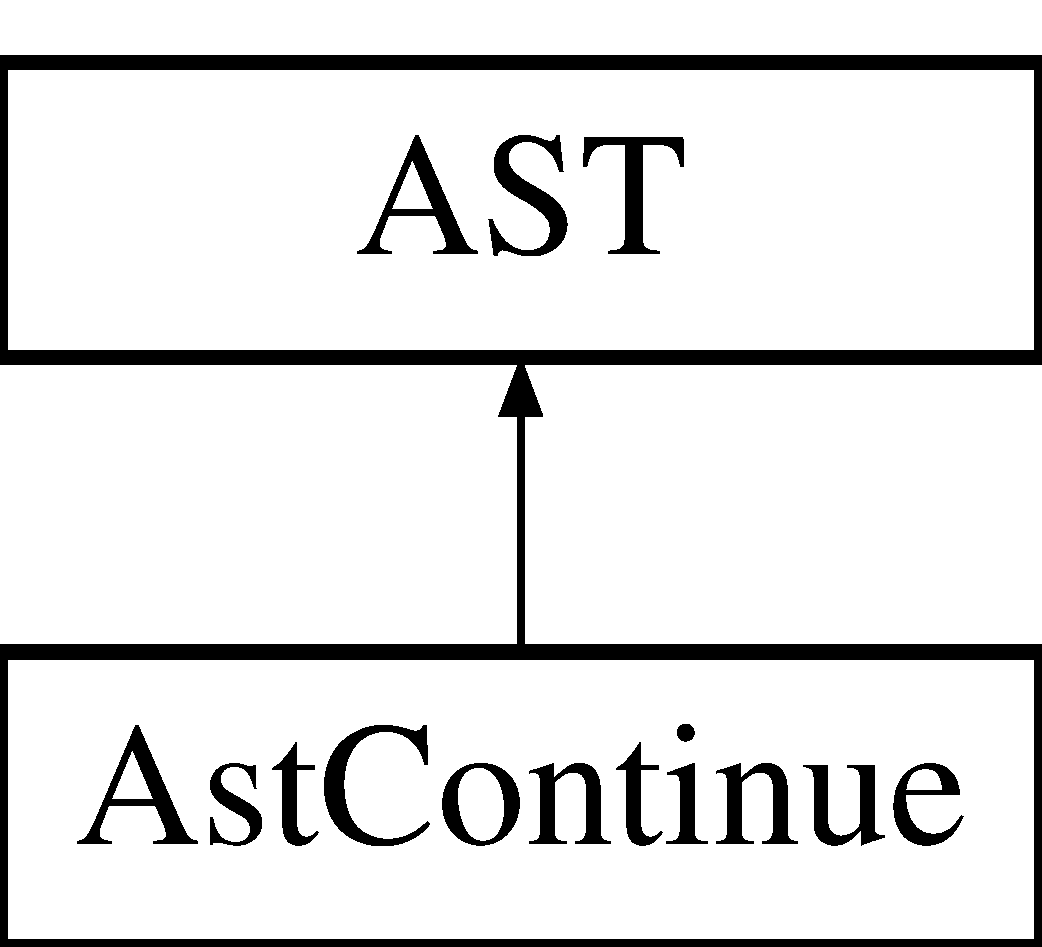
\includegraphics[height=2.000000cm]{classAstContinue}
\end{center}
\end{figure}
\subsection*{Public Member Functions}
\begin{DoxyCompactItemize}
\item 
void \hyperlink{classAstContinue_a5e3d13c7d6c9077f7a3d50683746c518}{Visit} ()
\begin{DoxyCompactList}\small\item\em This function is responsible for tree traversals. \end{DoxyCompactList}\item 
void \hyperlink{classAstContinue_a5e3d13c7d6c9077f7a3d50683746c518}{Visit} ()
\begin{DoxyCompactList}\small\item\em This function is responsible for tree traversals. \end{DoxyCompactList}\item 
void \hyperlink{classAstContinue_a5e3d13c7d6c9077f7a3d50683746c518}{Visit} ()
\begin{DoxyCompactList}\small\item\em This function is responsible for tree traversals. \end{DoxyCompactList}\item 
void \hyperlink{classAstContinue_a5e3d13c7d6c9077f7a3d50683746c518}{Visit} ()
\begin{DoxyCompactList}\small\item\em This function is responsible for tree traversals. \end{DoxyCompactList}\item 
void \hyperlink{classAST_a71d680856e95ff89f55d5311a552eba6}{set\-Label} (string l)
\begin{DoxyCompactList}\small\item\em Sets the label for the node. \end{DoxyCompactList}\item 
void \hyperlink{classAST_a71d680856e95ff89f55d5311a552eba6}{set\-Label} (string l)
\begin{DoxyCompactList}\small\item\em Sets the label for the node. \end{DoxyCompactList}\item 
void \hyperlink{classAST_a71d680856e95ff89f55d5311a552eba6}{set\-Label} (string l)
\begin{DoxyCompactList}\small\item\em Sets the label for the node. \end{DoxyCompactList}\item 
void \hyperlink{classAST_a71d680856e95ff89f55d5311a552eba6}{set\-Label} (string l)
\begin{DoxyCompactList}\small\item\em Sets the label for the node. \end{DoxyCompactList}\item 
int \hyperlink{classAST_ab7a5b1d9f1c2de0d98deb356f724a42c}{get\-U\-I\-D} ()
\begin{DoxyCompactList}\small\item\em Gets the node's unique I\-D. \end{DoxyCompactList}\item 
int \hyperlink{classAST_ab7a5b1d9f1c2de0d98deb356f724a42c}{get\-U\-I\-D} ()
\begin{DoxyCompactList}\small\item\em Gets the node's unique I\-D. \end{DoxyCompactList}\item 
int \hyperlink{classAST_ab7a5b1d9f1c2de0d98deb356f724a42c}{get\-U\-I\-D} ()
\begin{DoxyCompactList}\small\item\em Gets the node's unique I\-D. \end{DoxyCompactList}\item 
int \hyperlink{classAST_ab7a5b1d9f1c2de0d98deb356f724a42c}{get\-U\-I\-D} ()
\begin{DoxyCompactList}\small\item\em Gets the node's unique I\-D. \end{DoxyCompactList}\item 
string \hyperlink{classAST_aee029be902fffc927d16ccb03eb922ad}{get\-Label} ()
\begin{DoxyCompactList}\small\item\em Gets the node's label. \end{DoxyCompactList}\item 
string \hyperlink{classAST_aee029be902fffc927d16ccb03eb922ad}{get\-Label} ()
\begin{DoxyCompactList}\small\item\em Gets the node's label. \end{DoxyCompactList}\item 
string \hyperlink{classAST_aee029be902fffc927d16ccb03eb922ad}{get\-Label} ()
\begin{DoxyCompactList}\small\item\em Gets the node's label. \end{DoxyCompactList}\item 
string \hyperlink{classAST_aee029be902fffc927d16ccb03eb922ad}{get\-Label} ()
\begin{DoxyCompactList}\small\item\em Gets the node's label. \end{DoxyCompactList}\end{DoxyCompactItemize}
\subsection*{Public Attributes}
\begin{DoxyCompactItemize}
\item 
\hypertarget{classAST_aaf215802de409f8096c063d01ffa6783}{bool \hyperlink{classAST_aaf215802de409f8096c063d01ffa6783}{needs\-Cast}}\label{classAST_aaf215802de409f8096c063d01ffa6783}

\begin{DoxyCompactList}\small\item\em This indicates if cast 3\-A\-C needs to be output, and is only relevant for expressions. \end{DoxyCompactList}\item 
\hypertarget{classAST_afa9e77ef650ec6664458fa6cb55be985}{bool \hyperlink{classAST_afa9e77ef650ec6664458fa6cb55be985}{is\-Conv}}\label{classAST_afa9e77ef650ec6664458fa6cb55be985}

\begin{DoxyCompactList}\small\item\em Indicates is a conversion is possible. \end{DoxyCompactList}\item 
\hypertarget{classAST_a61ef3317e023d45237e06615b387cd6b}{C\-O\-N\-V\-E\-R\-S\-I\-O\-N\-T\-Y\-P\-E \hyperlink{classAST_a61ef3317e023d45237e06615b387cd6b}{conv\-Type}}\label{classAST_a61ef3317e023d45237e06615b387cd6b}

\begin{DoxyCompactList}\small\item\em If needs\-Cast is true, then this indicates what the cast should be. \end{DoxyCompactList}\item 
\hypertarget{classAST_aea9b07b39d24183f38c0029cec0a878e}{int \hyperlink{classAST_aea9b07b39d24183f38c0029cec0a878e}{operand\-To\-Cast}}\label{classAST_aea9b07b39d24183f38c0029cec0a878e}

\begin{DoxyCompactList}\small\item\em This indicates if the first or second operand should be the one that is cast. \end{DoxyCompactList}\end{DoxyCompactItemize}
\subsection*{Static Public Attributes}
\begin{DoxyCompactItemize}
\item 
\hypertarget{classAST_a5fdfd5f7b104dd92889163bdadbc68d6}{static \hyperlink{classVisualizer}{Visualizer} \hyperlink{classAST_a5fdfd5f7b104dd92889163bdadbc68d6}{vis}}\label{classAST_a5fdfd5f7b104dd92889163bdadbc68d6}

\begin{DoxyCompactList}\small\item\em Static visualizer instance for generating the visualization of the \hyperlink{classAST}{A\-S\-T}. \end{DoxyCompactList}\item 
\hypertarget{classAST_a8a3ace322f50e030331065d644ee55ee}{static \hyperlink{classTAC__Generator}{T\-A\-C\-\_\-\-Generator} \hyperlink{classAST_a8a3ace322f50e030331065d644ee55ee}{tac\-Gen}}\label{classAST_a8a3ace322f50e030331065d644ee55ee}

\begin{DoxyCompactList}\small\item\em Three address code generator. \end{DoxyCompactList}\item 
\hypertarget{classAST_a1f69448c6dc368d005631a128460083d}{static string {\bfseries current\-Temp} =\char`\"{}\char`\"{}}\label{classAST_a1f69448c6dc368d005631a128460083d}

\item 
\hypertarget{classAST_a551aec090c932ab69365238b40a8a4eb}{static string \hyperlink{classAST_a551aec090c932ab69365238b40a8a4eb}{return\-Label} =\char`\"{}\char`\"{}}\label{classAST_a551aec090c932ab69365238b40a8a4eb}

\begin{DoxyCompactList}\small\item\em This is for storing the string id of any temporary result register that may be created during 3\-A\-C generation. \end{DoxyCompactList}\item 
\hypertarget{classAST_a73c0a266df52be71e6b527b6aa635173}{static list$<$ string $>$ {\bfseries temp\-Stack}}\label{classAST_a73c0a266df52be71e6b527b6aa635173}

\item 
\hypertarget{classAST_abf9e84b541ff04b7bb64e6e4371512d4}{static string {\bfseries last\-I\-D} =\char`\"{}\char`\"{}}\label{classAST_abf9e84b541ff04b7bb64e6e4371512d4}

\item 
\hypertarget{classAST_a163003bfe9c30510ec8039870346049f}{static \hyperlink{classSymTab}{Sym\-Tab} $\ast$ {\bfseries symbol\-Table} =N\-U\-L\-L}\label{classAST_a163003bfe9c30510ec8039870346049f}

\item 
\hypertarget{classAST_a5c3cc894d9c0453523dec9ed76f18a04}{static string {\bfseries current\-Function} =\char`\"{}\char`\"{}}\label{classAST_a5c3cc894d9c0453523dec9ed76f18a04}

\item 
\hypertarget{classAST_a66155513b59ff1a04c8ece8b20ec31f5}{static int {\bfseries current\-Constant\-Value} =0}\label{classAST_a66155513b59ff1a04c8ece8b20ec31f5}

\item 
\hypertarget{classAST_a3d031d7bab635ba1f015aade5943f40c}{static string {\bfseries current\-Id\-Name} =\char`\"{}\char`\"{}}\label{classAST_a3d031d7bab635ba1f015aade5943f40c}

\item 
\hypertarget{classAST_a16c4b6e54febc1a26b31a64a46972ef0}{static int {\bfseries current\-Index\-Val} = 0}\label{classAST_a16c4b6e54febc1a26b31a64a46972ef0}

\item 
\hypertarget{classAST_a6fc65ae9dd064a88941d4b88669b19db}{static string {\bfseries current\-I\-D} = \char`\"{}\char`\"{}}\label{classAST_a6fc65ae9dd064a88941d4b88669b19db}

\end{DoxyCompactItemize}
\subsection*{Protected Attributes}
\begin{DoxyCompactItemize}
\item 
\hypertarget{classAST_a847b778f1c3dd5a19de32de432ee6e15}{int \hyperlink{classAST_a847b778f1c3dd5a19de32de432ee6e15}{uid}}\label{classAST_a847b778f1c3dd5a19de32de432ee6e15}

\begin{DoxyCompactList}\small\item\em The unique id. \end{DoxyCompactList}\item 
\hypertarget{classAST_ab2e239ccc0688d2341724432ff5a1a31}{string \hyperlink{classAST_ab2e239ccc0688d2341724432ff5a1a31}{label}}\label{classAST_ab2e239ccc0688d2341724432ff5a1a31}

\begin{DoxyCompactList}\small\item\em The label to be printed in the visualization. \end{DoxyCompactList}\end{DoxyCompactItemize}


\subsection{Detailed Description}


Definition at line 794 of file Ast.\-h.



\subsection{Member Function Documentation}
\hypertarget{classAST_aee029be902fffc927d16ccb03eb922ad}{\index{Ast\-Continue@{Ast\-Continue}!get\-Label@{get\-Label}}
\index{get\-Label@{get\-Label}!AstContinue@{Ast\-Continue}}
\subsubsection[{get\-Label}]{\setlength{\rightskip}{0pt plus 5cm}string A\-S\-T\-::get\-Label (
\begin{DoxyParamCaption}
{}
\end{DoxyParamCaption}
)\hspace{0.3cm}{\ttfamily [inline]}, {\ttfamily [inherited]}}}\label{classAST_aee029be902fffc927d16ccb03eb922ad}


Gets the node's label. 

\begin{DoxyReturn}{Returns}
The label 
\end{DoxyReturn}


Definition at line 60 of file Ast.\-h.

\hypertarget{classAST_aee029be902fffc927d16ccb03eb922ad}{\index{Ast\-Continue@{Ast\-Continue}!get\-Label@{get\-Label}}
\index{get\-Label@{get\-Label}!AstContinue@{Ast\-Continue}}
\subsubsection[{get\-Label}]{\setlength{\rightskip}{0pt plus 5cm}string A\-S\-T\-::get\-Label (
\begin{DoxyParamCaption}
{}
\end{DoxyParamCaption}
)\hspace{0.3cm}{\ttfamily [inline]}, {\ttfamily [inherited]}}}\label{classAST_aee029be902fffc927d16ccb03eb922ad}


Gets the node's label. 

\begin{DoxyReturn}{Returns}
The label 
\end{DoxyReturn}


Definition at line 60 of file C\-Scanner.\-ll.

\hypertarget{classAST_aee029be902fffc927d16ccb03eb922ad}{\index{Ast\-Continue@{Ast\-Continue}!get\-Label@{get\-Label}}
\index{get\-Label@{get\-Label}!AstContinue@{Ast\-Continue}}
\subsubsection[{get\-Label}]{\setlength{\rightskip}{0pt plus 5cm}string A\-S\-T\-::get\-Label (
\begin{DoxyParamCaption}
{}
\end{DoxyParamCaption}
)\hspace{0.3cm}{\ttfamily [inline]}, {\ttfamily [inherited]}}}\label{classAST_aee029be902fffc927d16ccb03eb922ad}


Gets the node's label. 

\begin{DoxyReturn}{Returns}
The label 
\end{DoxyReturn}


Definition at line 60 of file C\-Parser.\-yy.

\hypertarget{classAST_aee029be902fffc927d16ccb03eb922ad}{\index{Ast\-Continue@{Ast\-Continue}!get\-Label@{get\-Label}}
\index{get\-Label@{get\-Label}!AstContinue@{Ast\-Continue}}
\subsubsection[{get\-Label}]{\setlength{\rightskip}{0pt plus 5cm}string A\-S\-T\-::get\-Label (
\begin{DoxyParamCaption}
{}
\end{DoxyParamCaption}
)\hspace{0.3cm}{\ttfamily [inline]}, {\ttfamily [inherited]}}}\label{classAST_aee029be902fffc927d16ccb03eb922ad}


Gets the node's label. 

\begin{DoxyReturn}{Returns}
The label 
\end{DoxyReturn}


Definition at line 60 of file C\-Parser.\-yy.

\hypertarget{classAST_ab7a5b1d9f1c2de0d98deb356f724a42c}{\index{Ast\-Continue@{Ast\-Continue}!get\-U\-I\-D@{get\-U\-I\-D}}
\index{get\-U\-I\-D@{get\-U\-I\-D}!AstContinue@{Ast\-Continue}}
\subsubsection[{get\-U\-I\-D}]{\setlength{\rightskip}{0pt plus 5cm}int A\-S\-T\-::get\-U\-I\-D (
\begin{DoxyParamCaption}
{}
\end{DoxyParamCaption}
)\hspace{0.3cm}{\ttfamily [inline]}, {\ttfamily [inherited]}}}\label{classAST_ab7a5b1d9f1c2de0d98deb356f724a42c}


Gets the node's unique I\-D. 

\begin{DoxyReturn}{Returns}
The unique id 
\end{DoxyReturn}


Definition at line 53 of file C\-Parser.\-yy.

\hypertarget{classAST_ab7a5b1d9f1c2de0d98deb356f724a42c}{\index{Ast\-Continue@{Ast\-Continue}!get\-U\-I\-D@{get\-U\-I\-D}}
\index{get\-U\-I\-D@{get\-U\-I\-D}!AstContinue@{Ast\-Continue}}
\subsubsection[{get\-U\-I\-D}]{\setlength{\rightskip}{0pt plus 5cm}int A\-S\-T\-::get\-U\-I\-D (
\begin{DoxyParamCaption}
{}
\end{DoxyParamCaption}
)\hspace{0.3cm}{\ttfamily [inline]}, {\ttfamily [inherited]}}}\label{classAST_ab7a5b1d9f1c2de0d98deb356f724a42c}


Gets the node's unique I\-D. 

\begin{DoxyReturn}{Returns}
The unique id 
\end{DoxyReturn}


Definition at line 53 of file C\-Parser.\-yy.

\hypertarget{classAST_ab7a5b1d9f1c2de0d98deb356f724a42c}{\index{Ast\-Continue@{Ast\-Continue}!get\-U\-I\-D@{get\-U\-I\-D}}
\index{get\-U\-I\-D@{get\-U\-I\-D}!AstContinue@{Ast\-Continue}}
\subsubsection[{get\-U\-I\-D}]{\setlength{\rightskip}{0pt plus 5cm}int A\-S\-T\-::get\-U\-I\-D (
\begin{DoxyParamCaption}
{}
\end{DoxyParamCaption}
)\hspace{0.3cm}{\ttfamily [inline]}, {\ttfamily [inherited]}}}\label{classAST_ab7a5b1d9f1c2de0d98deb356f724a42c}


Gets the node's unique I\-D. 

\begin{DoxyReturn}{Returns}
The unique id 
\end{DoxyReturn}


Definition at line 53 of file C\-Scanner.\-ll.

\hypertarget{classAST_ab7a5b1d9f1c2de0d98deb356f724a42c}{\index{Ast\-Continue@{Ast\-Continue}!get\-U\-I\-D@{get\-U\-I\-D}}
\index{get\-U\-I\-D@{get\-U\-I\-D}!AstContinue@{Ast\-Continue}}
\subsubsection[{get\-U\-I\-D}]{\setlength{\rightskip}{0pt plus 5cm}int A\-S\-T\-::get\-U\-I\-D (
\begin{DoxyParamCaption}
{}
\end{DoxyParamCaption}
)\hspace{0.3cm}{\ttfamily [inline]}, {\ttfamily [inherited]}}}\label{classAST_ab7a5b1d9f1c2de0d98deb356f724a42c}


Gets the node's unique I\-D. 

\begin{DoxyReturn}{Returns}
The unique id 
\end{DoxyReturn}


Definition at line 53 of file Ast.\-h.

\hypertarget{classAST_a71d680856e95ff89f55d5311a552eba6}{\index{Ast\-Continue@{Ast\-Continue}!set\-Label@{set\-Label}}
\index{set\-Label@{set\-Label}!AstContinue@{Ast\-Continue}}
\subsubsection[{set\-Label}]{\setlength{\rightskip}{0pt plus 5cm}void A\-S\-T\-::set\-Label (
\begin{DoxyParamCaption}
\item[{string}]{l}
\end{DoxyParamCaption}
)\hspace{0.3cm}{\ttfamily [inline]}, {\ttfamily [inherited]}}}\label{classAST_a71d680856e95ff89f55d5311a552eba6}


Sets the label for the node. 


\begin{DoxyParams}{Parameters}
{\em l} & The label string \\
\hline
\end{DoxyParams}


Definition at line 43 of file C\-Scanner.\-ll.

\hypertarget{classAST_a71d680856e95ff89f55d5311a552eba6}{\index{Ast\-Continue@{Ast\-Continue}!set\-Label@{set\-Label}}
\index{set\-Label@{set\-Label}!AstContinue@{Ast\-Continue}}
\subsubsection[{set\-Label}]{\setlength{\rightskip}{0pt plus 5cm}void A\-S\-T\-::set\-Label (
\begin{DoxyParamCaption}
\item[{string}]{l}
\end{DoxyParamCaption}
)\hspace{0.3cm}{\ttfamily [inline]}, {\ttfamily [inherited]}}}\label{classAST_a71d680856e95ff89f55d5311a552eba6}


Sets the label for the node. 


\begin{DoxyParams}{Parameters}
{\em l} & The label string \\
\hline
\end{DoxyParams}


Definition at line 43 of file C\-Parser.\-yy.

\hypertarget{classAST_a71d680856e95ff89f55d5311a552eba6}{\index{Ast\-Continue@{Ast\-Continue}!set\-Label@{set\-Label}}
\index{set\-Label@{set\-Label}!AstContinue@{Ast\-Continue}}
\subsubsection[{set\-Label}]{\setlength{\rightskip}{0pt plus 5cm}void A\-S\-T\-::set\-Label (
\begin{DoxyParamCaption}
\item[{string}]{l}
\end{DoxyParamCaption}
)\hspace{0.3cm}{\ttfamily [inline]}, {\ttfamily [inherited]}}}\label{classAST_a71d680856e95ff89f55d5311a552eba6}


Sets the label for the node. 


\begin{DoxyParams}{Parameters}
{\em l} & The label string \\
\hline
\end{DoxyParams}


Definition at line 43 of file Ast.\-h.

\hypertarget{classAST_a71d680856e95ff89f55d5311a552eba6}{\index{Ast\-Continue@{Ast\-Continue}!set\-Label@{set\-Label}}
\index{set\-Label@{set\-Label}!AstContinue@{Ast\-Continue}}
\subsubsection[{set\-Label}]{\setlength{\rightskip}{0pt plus 5cm}void A\-S\-T\-::set\-Label (
\begin{DoxyParamCaption}
\item[{string}]{l}
\end{DoxyParamCaption}
)\hspace{0.3cm}{\ttfamily [inline]}, {\ttfamily [inherited]}}}\label{classAST_a71d680856e95ff89f55d5311a552eba6}


Sets the label for the node. 


\begin{DoxyParams}{Parameters}
{\em l} & The label string \\
\hline
\end{DoxyParams}


Definition at line 43 of file C\-Parser.\-yy.

\hypertarget{classAstContinue_a5e3d13c7d6c9077f7a3d50683746c518}{\index{Ast\-Continue@{Ast\-Continue}!Visit@{Visit}}
\index{Visit@{Visit}!AstContinue@{Ast\-Continue}}
\subsubsection[{Visit}]{\setlength{\rightskip}{0pt plus 5cm}void Ast\-Continue\-::\-Visit (
\begin{DoxyParamCaption}
{}
\end{DoxyParamCaption}
)\hspace{0.3cm}{\ttfamily [virtual]}}}\label{classAstContinue_a5e3d13c7d6c9077f7a3d50683746c518}


This function is responsible for tree traversals. 

This function will call the Visit functions of each of it's children nodes, call the visualization code for itself, and output any 3\-A\-C that can be generated at the current node. 

Reimplemented from \hyperlink{classAST_a5828cc86f2c4f1a0aeab6d7069e8fd82}{A\-S\-T}.



Definition at line 2143 of file Ast.\-cpp.

\hypertarget{classAstContinue_a5e3d13c7d6c9077f7a3d50683746c518}{\index{Ast\-Continue@{Ast\-Continue}!Visit@{Visit}}
\index{Visit@{Visit}!AstContinue@{Ast\-Continue}}
\subsubsection[{Visit}]{\setlength{\rightskip}{0pt plus 5cm}void Ast\-Continue\-::\-Visit (
\begin{DoxyParamCaption}
{}
\end{DoxyParamCaption}
)\hspace{0.3cm}{\ttfamily [virtual]}}}\label{classAstContinue_a5e3d13c7d6c9077f7a3d50683746c518}


This function is responsible for tree traversals. 

This function will call the Visit functions of each of it's children nodes, call the visualization code for itself, and output any 3\-A\-C that can be generated at the current node. 

Reimplemented from \hyperlink{classAST_a5828cc86f2c4f1a0aeab6d7069e8fd82}{A\-S\-T}.

\hypertarget{classAstContinue_a5e3d13c7d6c9077f7a3d50683746c518}{\index{Ast\-Continue@{Ast\-Continue}!Visit@{Visit}}
\index{Visit@{Visit}!AstContinue@{Ast\-Continue}}
\subsubsection[{Visit}]{\setlength{\rightskip}{0pt plus 5cm}void Ast\-Continue\-::\-Visit (
\begin{DoxyParamCaption}
{}
\end{DoxyParamCaption}
)\hspace{0.3cm}{\ttfamily [virtual]}}}\label{classAstContinue_a5e3d13c7d6c9077f7a3d50683746c518}


This function is responsible for tree traversals. 

This function will call the Visit functions of each of it's children nodes, call the visualization code for itself, and output any 3\-A\-C that can be generated at the current node. 

Reimplemented from \hyperlink{classAST_a5828cc86f2c4f1a0aeab6d7069e8fd82}{A\-S\-T}.

\hypertarget{classAstContinue_a5e3d13c7d6c9077f7a3d50683746c518}{\index{Ast\-Continue@{Ast\-Continue}!Visit@{Visit}}
\index{Visit@{Visit}!AstContinue@{Ast\-Continue}}
\subsubsection[{Visit}]{\setlength{\rightskip}{0pt plus 5cm}void Ast\-Continue\-::\-Visit (
\begin{DoxyParamCaption}
{}
\end{DoxyParamCaption}
)\hspace{0.3cm}{\ttfamily [virtual]}}}\label{classAstContinue_a5e3d13c7d6c9077f7a3d50683746c518}


This function is responsible for tree traversals. 

This function will call the Visit functions of each of it's children nodes, call the visualization code for itself, and output any 3\-A\-C that can be generated at the current node. 

Reimplemented from \hyperlink{classAST_a5828cc86f2c4f1a0aeab6d7069e8fd82}{A\-S\-T}.



The documentation for this class was generated from the following files\-:\begin{DoxyCompactItemize}
\item 
Ast.\-h\item 
Ast.\-cpp\end{DoxyCompactItemize}

\input{classAstDecl}
\hypertarget{classAstDeclarationList}{\section{Ast\-Declaration\-List Class Reference}
\label{classAstDeclarationList}\index{Ast\-Declaration\-List@{Ast\-Declaration\-List}}
}
Inheritance diagram for Ast\-Declaration\-List\-:\begin{figure}[H]
\begin{center}
\leavevmode
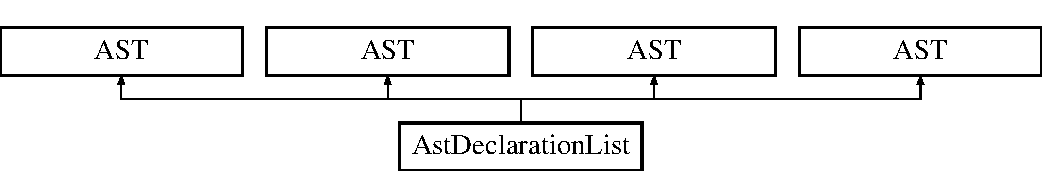
\includegraphics[height=2.000000cm]{classAstDeclarationList}
\end{center}
\end{figure}
\subsection*{Public Member Functions}
\begin{DoxyCompactItemize}
\item 
\hypertarget{classAstDeclarationList_a1c98628f55a26aabfacbbb670d2eac12}{void {\bfseries Visit} ()}\label{classAstDeclarationList_a1c98628f55a26aabfacbbb670d2eac12}

\item 
\hypertarget{classAST_a71d680856e95ff89f55d5311a552eba6}{void {\bfseries set\-Label} (string l)}\label{classAST_a71d680856e95ff89f55d5311a552eba6}

\item 
\hypertarget{classAST_ab7a5b1d9f1c2de0d98deb356f724a42c}{int {\bfseries get\-U\-I\-D} ()}\label{classAST_ab7a5b1d9f1c2de0d98deb356f724a42c}

\item 
\hypertarget{classAST_aee029be902fffc927d16ccb03eb922ad}{string {\bfseries get\-Label} ()}\label{classAST_aee029be902fffc927d16ccb03eb922ad}

\end{DoxyCompactItemize}
\subsection*{Static Public Attributes}
\begin{DoxyCompactItemize}
\item 
\hypertarget{classAST_aca9e6637209b31e03a09c0d42f29bdfa}{static \hyperlink{classVisualizer}{Visualizer} {\bfseries vis}}\label{classAST_aca9e6637209b31e03a09c0d42f29bdfa}

\end{DoxyCompactItemize}
\subsection*{Protected Attributes}
\begin{DoxyCompactItemize}
\item 
\hypertarget{classAST_a847b778f1c3dd5a19de32de432ee6e15}{int {\bfseries uid}}\label{classAST_a847b778f1c3dd5a19de32de432ee6e15}

\item 
\hypertarget{classAST_ab2e239ccc0688d2341724432ff5a1a31}{string {\bfseries label}}\label{classAST_ab2e239ccc0688d2341724432ff5a1a31}

\end{DoxyCompactItemize}


The documentation for this class was generated from the following file\-:\begin{DoxyCompactItemize}
\item 
Ast.\-h\end{DoxyCompactItemize}

\input{classAstDeclarator}
\input{classAstDeclList}
\input{classAstDecSpeci}
\input{classAstDirectAbsDecl}
\input{classAstDirectDecl}
\hypertarget{classAstDoWhile}{\section{Ast\-Do\-While Class Reference}
\label{classAstDoWhile}\index{Ast\-Do\-While@{Ast\-Do\-While}}
}
Inheritance diagram for Ast\-Do\-While\-:\begin{figure}[H]
\begin{center}
\leavevmode
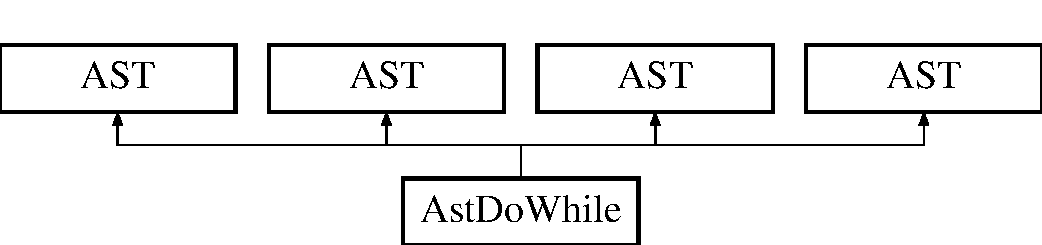
\includegraphics[height=2.000000cm]{classAstDoWhile}
\end{center}
\end{figure}
\subsection*{Public Member Functions}
\begin{DoxyCompactItemize}
\item 
\hypertarget{classAstDoWhile_a7a03e49e40bf03becd193a25be0302da}{{\bfseries Ast\-Do\-While} (\hyperlink{classAstStatement}{Ast\-Statement} $\ast$s, \hyperlink{classAstExpression}{Ast\-Expression} $\ast$t)}\label{classAstDoWhile_a7a03e49e40bf03becd193a25be0302da}

\item 
\hypertarget{classAstDoWhile_ae45111e771d2b16c5aef452cf37a629f}{void {\bfseries Visit} ()}\label{classAstDoWhile_ae45111e771d2b16c5aef452cf37a629f}

\item 
\hypertarget{classAST_a71d680856e95ff89f55d5311a552eba6}{void {\bfseries set\-Label} (string l)}\label{classAST_a71d680856e95ff89f55d5311a552eba6}

\item 
\hypertarget{classAST_ab7a5b1d9f1c2de0d98deb356f724a42c}{int {\bfseries get\-U\-I\-D} ()}\label{classAST_ab7a5b1d9f1c2de0d98deb356f724a42c}

\item 
\hypertarget{classAST_aee029be902fffc927d16ccb03eb922ad}{string {\bfseries get\-Label} ()}\label{classAST_aee029be902fffc927d16ccb03eb922ad}

\end{DoxyCompactItemize}
\subsection*{Static Public Attributes}
\begin{DoxyCompactItemize}
\item 
\hypertarget{classAST_aca9e6637209b31e03a09c0d42f29bdfa}{static \hyperlink{classVisualizer}{Visualizer} {\bfseries vis}}\label{classAST_aca9e6637209b31e03a09c0d42f29bdfa}

\end{DoxyCompactItemize}
\subsection*{Protected Attributes}
\begin{DoxyCompactItemize}
\item 
\hypertarget{classAST_a847b778f1c3dd5a19de32de432ee6e15}{int {\bfseries uid}}\label{classAST_a847b778f1c3dd5a19de32de432ee6e15}

\item 
\hypertarget{classAST_ab2e239ccc0688d2341724432ff5a1a31}{string {\bfseries label}}\label{classAST_ab2e239ccc0688d2341724432ff5a1a31}

\end{DoxyCompactItemize}
\subsection*{Private Attributes}
\begin{DoxyCompactItemize}
\item 
\hypertarget{classAstDoWhile_a178e28e21ffefcd0dd2106f13b35220a}{\hyperlink{classAstExpression}{Ast\-Expression} $\ast$ {\bfseries test}}\label{classAstDoWhile_a178e28e21ffefcd0dd2106f13b35220a}

\item 
\hypertarget{classAstDoWhile_afc6f50c748278c661be0e03d47f90db1}{\hyperlink{classAstStatement}{Ast\-Statement} $\ast$ {\bfseries statement}}\label{classAstDoWhile_afc6f50c748278c661be0e03d47f90db1}

\end{DoxyCompactItemize}


The documentation for this class was generated from the following files\-:\begin{DoxyCompactItemize}
\item 
Ast.\-h\item 
Ast.\-cpp\end{DoxyCompactItemize}

\input{classAstEnumerator}
\input{classAstEnumList}
\hypertarget{classAstEqExpr}{\section{Ast\-Eq\-Expr Class Reference}
\label{classAstEqExpr}\index{Ast\-Eq\-Expr@{Ast\-Eq\-Expr}}
}
Inheritance diagram for Ast\-Eq\-Expr\-:\begin{figure}[H]
\begin{center}
\leavevmode
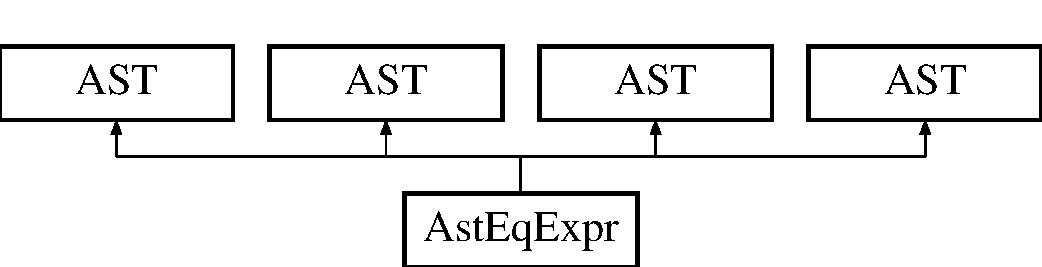
\includegraphics[height=2.000000cm]{classAstEqExpr}
\end{center}
\end{figure}
\subsection*{Public Types}
\begin{DoxyCompactItemize}
\item 
enum {\bfseries Operator} \{ {\bfseries N\-O\-N\-E}, 
{\bfseries E\-Q\-\_\-\-O\-P}, 
{\bfseries N\-E\-\_\-\-O\-P}
 \}
\end{DoxyCompactItemize}
\subsection*{Public Member Functions}
\begin{DoxyCompactItemize}
\item 
\hypertarget{classAstEqExpr_ae59f45e93845f531132980db8e8b8e2b}{{\bfseries Ast\-Eq\-Expr} (\hyperlink{classAstRelExpr}{Ast\-Rel\-Expr} $\ast$r)}\label{classAstEqExpr_ae59f45e93845f531132980db8e8b8e2b}

\item 
\hypertarget{classAstEqExpr_aac47a62e5410c55ac1f645a699e05ec4}{{\bfseries Ast\-Eq\-Expr} (\hyperlink{classAstEqExpr}{Ast\-Eq\-Expr} $\ast$e, Operator o, \hyperlink{classAstRelExpr}{Ast\-Rel\-Expr} $\ast$r)}\label{classAstEqExpr_aac47a62e5410c55ac1f645a699e05ec4}

\item 
void \hyperlink{classAstEqExpr_a6e0e9e88f6801eb135efef5bb5fe2851}{Visit} ()
\begin{DoxyCompactList}\small\item\em This function is responsible for tree traversals. \end{DoxyCompactList}\item 
void \hyperlink{classAST_a71d680856e95ff89f55d5311a552eba6}{set\-Label} (string l)
\begin{DoxyCompactList}\small\item\em Sets the label for the node. \end{DoxyCompactList}\item 
int \hyperlink{classAST_ab7a5b1d9f1c2de0d98deb356f724a42c}{get\-U\-I\-D} ()
\begin{DoxyCompactList}\small\item\em Gets the node's unique I\-D. \end{DoxyCompactList}\item 
string \hyperlink{classAST_aee029be902fffc927d16ccb03eb922ad}{get\-Label} ()
\begin{DoxyCompactList}\small\item\em Gets the node's label. \end{DoxyCompactList}\end{DoxyCompactItemize}
\subsection*{Public Attributes}
\begin{DoxyCompactItemize}
\item 
\hypertarget{classAstEqExpr_a33d1f50f34d77c20226b92f92112aa56}{enum Ast\-Eq\-Expr\-::\-Operator {\bfseries op}}\label{classAstEqExpr_a33d1f50f34d77c20226b92f92112aa56}

\end{DoxyCompactItemize}
\subsection*{Static Public Attributes}
\begin{DoxyCompactItemize}
\item 
\hypertarget{classAST_aca9e6637209b31e03a09c0d42f29bdfa}{static \hyperlink{classVisualizer}{Visualizer} \hyperlink{classAST_aca9e6637209b31e03a09c0d42f29bdfa}{vis}}\label{classAST_aca9e6637209b31e03a09c0d42f29bdfa}

\begin{DoxyCompactList}\small\item\em Static visualizer instance for generating the visualization of the \hyperlink{classAST}{A\-S\-T}. \end{DoxyCompactList}\end{DoxyCompactItemize}
\subsection*{Protected Attributes}
\begin{DoxyCompactItemize}
\item 
\hypertarget{classAST_a847b778f1c3dd5a19de32de432ee6e15}{int \hyperlink{classAST_a847b778f1c3dd5a19de32de432ee6e15}{uid}}\label{classAST_a847b778f1c3dd5a19de32de432ee6e15}

\begin{DoxyCompactList}\small\item\em The unique id. \end{DoxyCompactList}\item 
\hypertarget{classAST_ab2e239ccc0688d2341724432ff5a1a31}{string \hyperlink{classAST_ab2e239ccc0688d2341724432ff5a1a31}{label}}\label{classAST_ab2e239ccc0688d2341724432ff5a1a31}

\begin{DoxyCompactList}\small\item\em The label to be printed in the visualization. \end{DoxyCompactList}\end{DoxyCompactItemize}
\subsection*{Private Attributes}
\begin{DoxyCompactItemize}
\item 
\hypertarget{classAstEqExpr_a401f58facf1b9d58e6a6eb1cdb3cb38d}{\hyperlink{classAstRelExpr}{Ast\-Rel\-Expr} $\ast$ {\bfseries rel}}\label{classAstEqExpr_a401f58facf1b9d58e6a6eb1cdb3cb38d}

\item 
\hypertarget{classAstEqExpr_a66192b3d4a06af9796d6d34aa89bb8c7}{\hyperlink{classAstEqExpr}{Ast\-Eq\-Expr} $\ast$ {\bfseries eq}}\label{classAstEqExpr_a66192b3d4a06af9796d6d34aa89bb8c7}

\end{DoxyCompactItemize}


\subsection{Member Function Documentation}
\hypertarget{classAST_aee029be902fffc927d16ccb03eb922ad}{\index{Ast\-Eq\-Expr@{Ast\-Eq\-Expr}!get\-Label@{get\-Label}}
\index{get\-Label@{get\-Label}!AstEqExpr@{Ast\-Eq\-Expr}}
\subsubsection[{get\-Label}]{\setlength{\rightskip}{0pt plus 5cm}string A\-S\-T\-::get\-Label (
\begin{DoxyParamCaption}
{}
\end{DoxyParamCaption}
)\hspace{0.3cm}{\ttfamily [inline]}, {\ttfamily [inherited]}}}\label{classAST_aee029be902fffc927d16ccb03eb922ad}


Gets the node's label. 

\begin{DoxyReturn}{Returns}
The label 
\end{DoxyReturn}
\hypertarget{classAST_ab7a5b1d9f1c2de0d98deb356f724a42c}{\index{Ast\-Eq\-Expr@{Ast\-Eq\-Expr}!get\-U\-I\-D@{get\-U\-I\-D}}
\index{get\-U\-I\-D@{get\-U\-I\-D}!AstEqExpr@{Ast\-Eq\-Expr}}
\subsubsection[{get\-U\-I\-D}]{\setlength{\rightskip}{0pt plus 5cm}int A\-S\-T\-::get\-U\-I\-D (
\begin{DoxyParamCaption}
{}
\end{DoxyParamCaption}
)\hspace{0.3cm}{\ttfamily [inline]}, {\ttfamily [inherited]}}}\label{classAST_ab7a5b1d9f1c2de0d98deb356f724a42c}


Gets the node's unique I\-D. 

\begin{DoxyReturn}{Returns}
The unique id 
\end{DoxyReturn}
\hypertarget{classAST_a71d680856e95ff89f55d5311a552eba6}{\index{Ast\-Eq\-Expr@{Ast\-Eq\-Expr}!set\-Label@{set\-Label}}
\index{set\-Label@{set\-Label}!AstEqExpr@{Ast\-Eq\-Expr}}
\subsubsection[{set\-Label}]{\setlength{\rightskip}{0pt plus 5cm}void A\-S\-T\-::set\-Label (
\begin{DoxyParamCaption}
\item[{string}]{l}
\end{DoxyParamCaption}
)\hspace{0.3cm}{\ttfamily [inline]}, {\ttfamily [inherited]}}}\label{classAST_a71d680856e95ff89f55d5311a552eba6}


Sets the label for the node. 


\begin{DoxyParams}{Parameters}
{\em l} & The label string \\
\hline
\end{DoxyParams}
\hypertarget{classAstEqExpr_a6e0e9e88f6801eb135efef5bb5fe2851}{\index{Ast\-Eq\-Expr@{Ast\-Eq\-Expr}!Visit@{Visit}}
\index{Visit@{Visit}!AstEqExpr@{Ast\-Eq\-Expr}}
\subsubsection[{Visit}]{\setlength{\rightskip}{0pt plus 5cm}void Ast\-Eq\-Expr\-::\-Visit (
\begin{DoxyParamCaption}
{}
\end{DoxyParamCaption}
)\hspace{0.3cm}{\ttfamily [virtual]}}}\label{classAstEqExpr_a6e0e9e88f6801eb135efef5bb5fe2851}


This function is responsible for tree traversals. 

This function will call the Visit functions of each of it's children nodes, call the visualization code for itself, and output any 3\-A\-C that can be generated at the current node. 

Reimplemented from \hyperlink{classAST_a5828cc86f2c4f1a0aeab6d7069e8fd82}{A\-S\-T}.



The documentation for this class was generated from the following files\-:\begin{DoxyCompactItemize}
\item 
Ast.\-h\item 
Ast.\-cpp\end{DoxyCompactItemize}

\hypertarget{classAstExpression}{\section{Ast\-Expression Class Reference}
\label{classAstExpression}\index{Ast\-Expression@{Ast\-Expression}}
}
Inheritance diagram for Ast\-Expression\-:\begin{figure}[H]
\begin{center}
\leavevmode
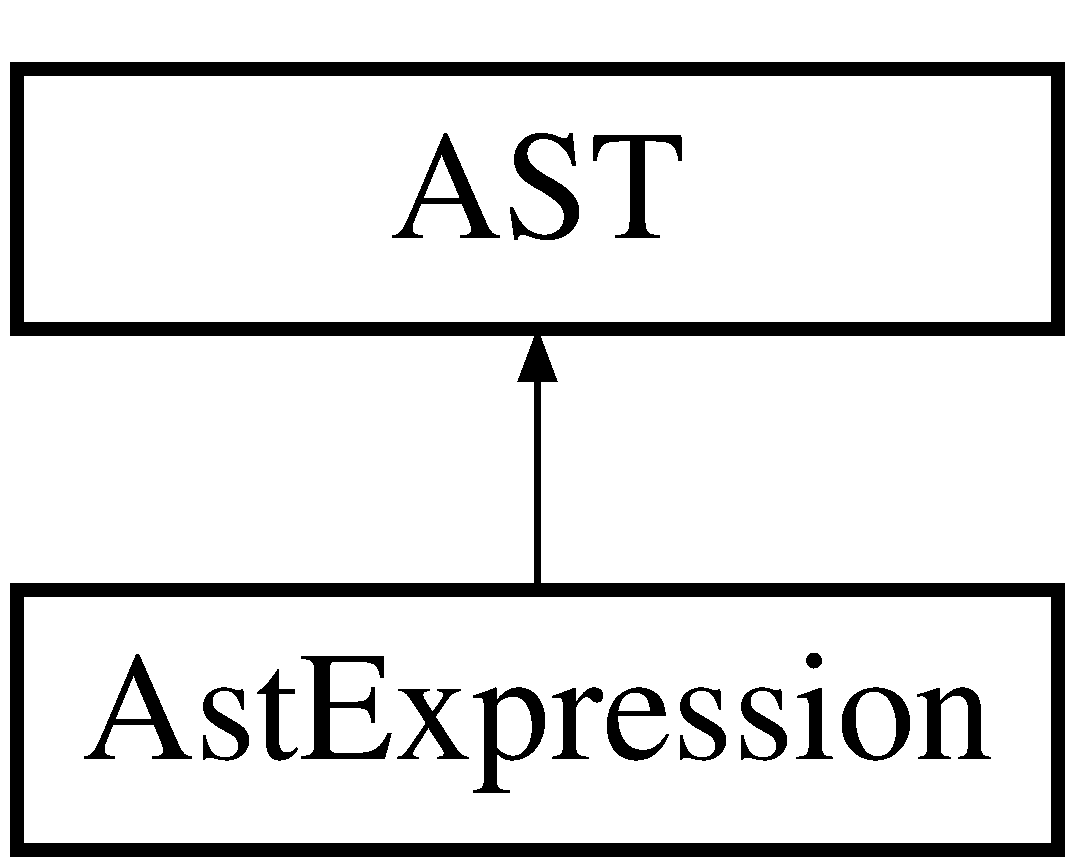
\includegraphics[height=2.000000cm]{classAstExpression}
\end{center}
\end{figure}
\subsection*{Public Member Functions}
\begin{DoxyCompactItemize}
\item 
\hypertarget{classAstExpression_a6c2ed06162eed9d5c420b3d3d0b1c5e4}{{\bfseries Ast\-Expression} (\hyperlink{classAstAssignExpr}{Ast\-Assign\-Expr} $\ast$a)}\label{classAstExpression_a6c2ed06162eed9d5c420b3d3d0b1c5e4}

\item 
\hypertarget{classAstExpression_ad02546e8d2ef52f3f2fb11baa95abdeb}{{\bfseries Ast\-Expression} (\hyperlink{classAstExpression}{Ast\-Expression} $\ast$e, \hyperlink{classAstAssignExpr}{Ast\-Assign\-Expr} $\ast$a)}\label{classAstExpression_ad02546e8d2ef52f3f2fb11baa95abdeb}

\item 
void \hyperlink{classAstExpression_acee231d1cd8e4c92393f023bc2f1ecf2}{Visit} ()
\begin{DoxyCompactList}\small\item\em This function is responsible for tree traversals. \end{DoxyCompactList}\item 
\hypertarget{classAstExpression_a6c2ed06162eed9d5c420b3d3d0b1c5e4}{{\bfseries Ast\-Expression} (\hyperlink{classAstAssignExpr}{Ast\-Assign\-Expr} $\ast$a)}\label{classAstExpression_a6c2ed06162eed9d5c420b3d3d0b1c5e4}

\item 
\hypertarget{classAstExpression_ad02546e8d2ef52f3f2fb11baa95abdeb}{{\bfseries Ast\-Expression} (\hyperlink{classAstExpression}{Ast\-Expression} $\ast$e, \hyperlink{classAstAssignExpr}{Ast\-Assign\-Expr} $\ast$a)}\label{classAstExpression_ad02546e8d2ef52f3f2fb11baa95abdeb}

\item 
void \hyperlink{classAstExpression_acee231d1cd8e4c92393f023bc2f1ecf2}{Visit} ()
\begin{DoxyCompactList}\small\item\em This function is responsible for tree traversals. \end{DoxyCompactList}\item 
\hypertarget{classAstExpression_a6c2ed06162eed9d5c420b3d3d0b1c5e4}{{\bfseries Ast\-Expression} (\hyperlink{classAstAssignExpr}{Ast\-Assign\-Expr} $\ast$a)}\label{classAstExpression_a6c2ed06162eed9d5c420b3d3d0b1c5e4}

\item 
\hypertarget{classAstExpression_ad02546e8d2ef52f3f2fb11baa95abdeb}{{\bfseries Ast\-Expression} (\hyperlink{classAstExpression}{Ast\-Expression} $\ast$e, \hyperlink{classAstAssignExpr}{Ast\-Assign\-Expr} $\ast$a)}\label{classAstExpression_ad02546e8d2ef52f3f2fb11baa95abdeb}

\item 
void \hyperlink{classAstExpression_acee231d1cd8e4c92393f023bc2f1ecf2}{Visit} ()
\begin{DoxyCompactList}\small\item\em This function is responsible for tree traversals. \end{DoxyCompactList}\item 
\hypertarget{classAstExpression_a6c2ed06162eed9d5c420b3d3d0b1c5e4}{{\bfseries Ast\-Expression} (\hyperlink{classAstAssignExpr}{Ast\-Assign\-Expr} $\ast$a)}\label{classAstExpression_a6c2ed06162eed9d5c420b3d3d0b1c5e4}

\item 
\hypertarget{classAstExpression_ad02546e8d2ef52f3f2fb11baa95abdeb}{{\bfseries Ast\-Expression} (\hyperlink{classAstExpression}{Ast\-Expression} $\ast$e, \hyperlink{classAstAssignExpr}{Ast\-Assign\-Expr} $\ast$a)}\label{classAstExpression_ad02546e8d2ef52f3f2fb11baa95abdeb}

\item 
void \hyperlink{classAstExpression_acee231d1cd8e4c92393f023bc2f1ecf2}{Visit} ()
\begin{DoxyCompactList}\small\item\em This function is responsible for tree traversals. \end{DoxyCompactList}\item 
void \hyperlink{classAST_a71d680856e95ff89f55d5311a552eba6}{set\-Label} (string l)
\begin{DoxyCompactList}\small\item\em Sets the label for the node. \end{DoxyCompactList}\item 
void \hyperlink{classAST_a71d680856e95ff89f55d5311a552eba6}{set\-Label} (string l)
\begin{DoxyCompactList}\small\item\em Sets the label for the node. \end{DoxyCompactList}\item 
void \hyperlink{classAST_a71d680856e95ff89f55d5311a552eba6}{set\-Label} (string l)
\begin{DoxyCompactList}\small\item\em Sets the label for the node. \end{DoxyCompactList}\item 
void \hyperlink{classAST_a71d680856e95ff89f55d5311a552eba6}{set\-Label} (string l)
\begin{DoxyCompactList}\small\item\em Sets the label for the node. \end{DoxyCompactList}\item 
int \hyperlink{classAST_ab7a5b1d9f1c2de0d98deb356f724a42c}{get\-U\-I\-D} ()
\begin{DoxyCompactList}\small\item\em Gets the node's unique I\-D. \end{DoxyCompactList}\item 
int \hyperlink{classAST_ab7a5b1d9f1c2de0d98deb356f724a42c}{get\-U\-I\-D} ()
\begin{DoxyCompactList}\small\item\em Gets the node's unique I\-D. \end{DoxyCompactList}\item 
int \hyperlink{classAST_ab7a5b1d9f1c2de0d98deb356f724a42c}{get\-U\-I\-D} ()
\begin{DoxyCompactList}\small\item\em Gets the node's unique I\-D. \end{DoxyCompactList}\item 
int \hyperlink{classAST_ab7a5b1d9f1c2de0d98deb356f724a42c}{get\-U\-I\-D} ()
\begin{DoxyCompactList}\small\item\em Gets the node's unique I\-D. \end{DoxyCompactList}\item 
string \hyperlink{classAST_aee029be902fffc927d16ccb03eb922ad}{get\-Label} ()
\begin{DoxyCompactList}\small\item\em Gets the node's label. \end{DoxyCompactList}\item 
string \hyperlink{classAST_aee029be902fffc927d16ccb03eb922ad}{get\-Label} ()
\begin{DoxyCompactList}\small\item\em Gets the node's label. \end{DoxyCompactList}\item 
string \hyperlink{classAST_aee029be902fffc927d16ccb03eb922ad}{get\-Label} ()
\begin{DoxyCompactList}\small\item\em Gets the node's label. \end{DoxyCompactList}\item 
string \hyperlink{classAST_aee029be902fffc927d16ccb03eb922ad}{get\-Label} ()
\begin{DoxyCompactList}\small\item\em Gets the node's label. \end{DoxyCompactList}\end{DoxyCompactItemize}
\subsection*{Public Attributes}
\begin{DoxyCompactItemize}
\item 
\hypertarget{classAstExpression_a2d074ab4d8ae2bfc86bbe9f69cf65ab9}{\hyperlink{classType}{Type} $\ast$ {\bfseries type}}\label{classAstExpression_a2d074ab4d8ae2bfc86bbe9f69cf65ab9}

\item 
\hypertarget{classAST_aaf215802de409f8096c063d01ffa6783}{bool \hyperlink{classAST_aaf215802de409f8096c063d01ffa6783}{needs\-Cast}}\label{classAST_aaf215802de409f8096c063d01ffa6783}

\begin{DoxyCompactList}\small\item\em This indicates if cast 3\-A\-C needs to be output, and is only relevant for expressions. \end{DoxyCompactList}\item 
\hypertarget{classAST_afa9e77ef650ec6664458fa6cb55be985}{bool \hyperlink{classAST_afa9e77ef650ec6664458fa6cb55be985}{is\-Conv}}\label{classAST_afa9e77ef650ec6664458fa6cb55be985}

\begin{DoxyCompactList}\small\item\em Indicates is a conversion is possible. \end{DoxyCompactList}\item 
\hypertarget{classAST_a61ef3317e023d45237e06615b387cd6b}{C\-O\-N\-V\-E\-R\-S\-I\-O\-N\-T\-Y\-P\-E \hyperlink{classAST_a61ef3317e023d45237e06615b387cd6b}{conv\-Type}}\label{classAST_a61ef3317e023d45237e06615b387cd6b}

\begin{DoxyCompactList}\small\item\em If needs\-Cast is true, then this indicates what the cast should be. \end{DoxyCompactList}\item 
\hypertarget{classAST_aea9b07b39d24183f38c0029cec0a878e}{int \hyperlink{classAST_aea9b07b39d24183f38c0029cec0a878e}{operand\-To\-Cast}}\label{classAST_aea9b07b39d24183f38c0029cec0a878e}

\begin{DoxyCompactList}\small\item\em This indicates if the first or second operand should be the one that is cast. \end{DoxyCompactList}\end{DoxyCompactItemize}
\subsection*{Static Public Attributes}
\begin{DoxyCompactItemize}
\item 
\hypertarget{classAST_a5fdfd5f7b104dd92889163bdadbc68d6}{static \hyperlink{classVisualizer}{Visualizer} \hyperlink{classAST_a5fdfd5f7b104dd92889163bdadbc68d6}{vis}}\label{classAST_a5fdfd5f7b104dd92889163bdadbc68d6}

\begin{DoxyCompactList}\small\item\em Static visualizer instance for generating the visualization of the \hyperlink{classAST}{A\-S\-T}. \end{DoxyCompactList}\item 
\hypertarget{classAST_a8a3ace322f50e030331065d644ee55ee}{static \hyperlink{classTAC__Generator}{T\-A\-C\-\_\-\-Generator} \hyperlink{classAST_a8a3ace322f50e030331065d644ee55ee}{tac\-Gen}}\label{classAST_a8a3ace322f50e030331065d644ee55ee}

\begin{DoxyCompactList}\small\item\em Three address code generator. \end{DoxyCompactList}\item 
\hypertarget{classAST_a1f69448c6dc368d005631a128460083d}{static string {\bfseries current\-Temp} =\char`\"{}\char`\"{}}\label{classAST_a1f69448c6dc368d005631a128460083d}

\item 
\hypertarget{classAST_a551aec090c932ab69365238b40a8a4eb}{static string \hyperlink{classAST_a551aec090c932ab69365238b40a8a4eb}{return\-Label} =\char`\"{}\char`\"{}}\label{classAST_a551aec090c932ab69365238b40a8a4eb}

\begin{DoxyCompactList}\small\item\em This is for storing the string id of any temporary result register that may be created during 3\-A\-C generation. \end{DoxyCompactList}\item 
\hypertarget{classAST_a73c0a266df52be71e6b527b6aa635173}{static list$<$ string $>$ {\bfseries temp\-Stack}}\label{classAST_a73c0a266df52be71e6b527b6aa635173}

\item 
\hypertarget{classAST_abf9e84b541ff04b7bb64e6e4371512d4}{static string {\bfseries last\-I\-D} =\char`\"{}\char`\"{}}\label{classAST_abf9e84b541ff04b7bb64e6e4371512d4}

\item 
\hypertarget{classAST_a163003bfe9c30510ec8039870346049f}{static \hyperlink{classSymTab}{Sym\-Tab} $\ast$ {\bfseries symbol\-Table} =N\-U\-L\-L}\label{classAST_a163003bfe9c30510ec8039870346049f}

\item 
\hypertarget{classAST_a5c3cc894d9c0453523dec9ed76f18a04}{static string {\bfseries current\-Function} =\char`\"{}\char`\"{}}\label{classAST_a5c3cc894d9c0453523dec9ed76f18a04}

\item 
\hypertarget{classAST_a66155513b59ff1a04c8ece8b20ec31f5}{static int {\bfseries current\-Constant\-Value} =0}\label{classAST_a66155513b59ff1a04c8ece8b20ec31f5}

\item 
\hypertarget{classAST_a3d031d7bab635ba1f015aade5943f40c}{static string {\bfseries current\-Id\-Name} =\char`\"{}\char`\"{}}\label{classAST_a3d031d7bab635ba1f015aade5943f40c}

\item 
\hypertarget{classAST_a16c4b6e54febc1a26b31a64a46972ef0}{static int {\bfseries current\-Index\-Val} = 0}\label{classAST_a16c4b6e54febc1a26b31a64a46972ef0}

\item 
\hypertarget{classAST_a6fc65ae9dd064a88941d4b88669b19db}{static string {\bfseries current\-I\-D} = \char`\"{}\char`\"{}}\label{classAST_a6fc65ae9dd064a88941d4b88669b19db}

\end{DoxyCompactItemize}
\subsection*{Protected Attributes}
\begin{DoxyCompactItemize}
\item 
\hypertarget{classAST_a847b778f1c3dd5a19de32de432ee6e15}{int \hyperlink{classAST_a847b778f1c3dd5a19de32de432ee6e15}{uid}}\label{classAST_a847b778f1c3dd5a19de32de432ee6e15}

\begin{DoxyCompactList}\small\item\em The unique id. \end{DoxyCompactList}\item 
\hypertarget{classAST_ab2e239ccc0688d2341724432ff5a1a31}{string \hyperlink{classAST_ab2e239ccc0688d2341724432ff5a1a31}{label}}\label{classAST_ab2e239ccc0688d2341724432ff5a1a31}

\begin{DoxyCompactList}\small\item\em The label to be printed in the visualization. \end{DoxyCompactList}\end{DoxyCompactItemize}
\subsection*{Private Attributes}
\begin{DoxyCompactItemize}
\item 
\hypertarget{classAstExpression_a73b9c481ce50852cc74ea7b6a49c46fd}{\hyperlink{classAstAssignExpr}{Ast\-Assign\-Expr} $\ast$ {\bfseries ass}}\label{classAstExpression_a73b9c481ce50852cc74ea7b6a49c46fd}

\item 
\hypertarget{classAstExpression_ad9a6f6870365ba7f8ae54b2fa58c0bea}{\hyperlink{classAstExpression}{Ast\-Expression} $\ast$ {\bfseries expr}}\label{classAstExpression_ad9a6f6870365ba7f8ae54b2fa58c0bea}

\end{DoxyCompactItemize}


\subsection{Detailed Description}


Definition at line 770 of file Ast.\-h.



\subsection{Member Function Documentation}
\hypertarget{classAST_aee029be902fffc927d16ccb03eb922ad}{\index{Ast\-Expression@{Ast\-Expression}!get\-Label@{get\-Label}}
\index{get\-Label@{get\-Label}!AstExpression@{Ast\-Expression}}
\subsubsection[{get\-Label}]{\setlength{\rightskip}{0pt plus 5cm}string A\-S\-T\-::get\-Label (
\begin{DoxyParamCaption}
{}
\end{DoxyParamCaption}
)\hspace{0.3cm}{\ttfamily [inline]}, {\ttfamily [inherited]}}}\label{classAST_aee029be902fffc927d16ccb03eb922ad}


Gets the node's label. 

\begin{DoxyReturn}{Returns}
The label 
\end{DoxyReturn}


Definition at line 60 of file Ast.\-h.

\hypertarget{classAST_aee029be902fffc927d16ccb03eb922ad}{\index{Ast\-Expression@{Ast\-Expression}!get\-Label@{get\-Label}}
\index{get\-Label@{get\-Label}!AstExpression@{Ast\-Expression}}
\subsubsection[{get\-Label}]{\setlength{\rightskip}{0pt plus 5cm}string A\-S\-T\-::get\-Label (
\begin{DoxyParamCaption}
{}
\end{DoxyParamCaption}
)\hspace{0.3cm}{\ttfamily [inline]}, {\ttfamily [inherited]}}}\label{classAST_aee029be902fffc927d16ccb03eb922ad}


Gets the node's label. 

\begin{DoxyReturn}{Returns}
The label 
\end{DoxyReturn}


Definition at line 60 of file C\-Scanner.\-ll.

\hypertarget{classAST_aee029be902fffc927d16ccb03eb922ad}{\index{Ast\-Expression@{Ast\-Expression}!get\-Label@{get\-Label}}
\index{get\-Label@{get\-Label}!AstExpression@{Ast\-Expression}}
\subsubsection[{get\-Label}]{\setlength{\rightskip}{0pt plus 5cm}string A\-S\-T\-::get\-Label (
\begin{DoxyParamCaption}
{}
\end{DoxyParamCaption}
)\hspace{0.3cm}{\ttfamily [inline]}, {\ttfamily [inherited]}}}\label{classAST_aee029be902fffc927d16ccb03eb922ad}


Gets the node's label. 

\begin{DoxyReturn}{Returns}
The label 
\end{DoxyReturn}


Definition at line 60 of file C\-Parser.\-yy.

\hypertarget{classAST_aee029be902fffc927d16ccb03eb922ad}{\index{Ast\-Expression@{Ast\-Expression}!get\-Label@{get\-Label}}
\index{get\-Label@{get\-Label}!AstExpression@{Ast\-Expression}}
\subsubsection[{get\-Label}]{\setlength{\rightskip}{0pt plus 5cm}string A\-S\-T\-::get\-Label (
\begin{DoxyParamCaption}
{}
\end{DoxyParamCaption}
)\hspace{0.3cm}{\ttfamily [inline]}, {\ttfamily [inherited]}}}\label{classAST_aee029be902fffc927d16ccb03eb922ad}


Gets the node's label. 

\begin{DoxyReturn}{Returns}
The label 
\end{DoxyReturn}


Definition at line 60 of file C\-Parser.\-yy.

\hypertarget{classAST_ab7a5b1d9f1c2de0d98deb356f724a42c}{\index{Ast\-Expression@{Ast\-Expression}!get\-U\-I\-D@{get\-U\-I\-D}}
\index{get\-U\-I\-D@{get\-U\-I\-D}!AstExpression@{Ast\-Expression}}
\subsubsection[{get\-U\-I\-D}]{\setlength{\rightskip}{0pt plus 5cm}int A\-S\-T\-::get\-U\-I\-D (
\begin{DoxyParamCaption}
{}
\end{DoxyParamCaption}
)\hspace{0.3cm}{\ttfamily [inline]}, {\ttfamily [inherited]}}}\label{classAST_ab7a5b1d9f1c2de0d98deb356f724a42c}


Gets the node's unique I\-D. 

\begin{DoxyReturn}{Returns}
The unique id 
\end{DoxyReturn}


Definition at line 53 of file C\-Parser.\-yy.

\hypertarget{classAST_ab7a5b1d9f1c2de0d98deb356f724a42c}{\index{Ast\-Expression@{Ast\-Expression}!get\-U\-I\-D@{get\-U\-I\-D}}
\index{get\-U\-I\-D@{get\-U\-I\-D}!AstExpression@{Ast\-Expression}}
\subsubsection[{get\-U\-I\-D}]{\setlength{\rightskip}{0pt plus 5cm}int A\-S\-T\-::get\-U\-I\-D (
\begin{DoxyParamCaption}
{}
\end{DoxyParamCaption}
)\hspace{0.3cm}{\ttfamily [inline]}, {\ttfamily [inherited]}}}\label{classAST_ab7a5b1d9f1c2de0d98deb356f724a42c}


Gets the node's unique I\-D. 

\begin{DoxyReturn}{Returns}
The unique id 
\end{DoxyReturn}


Definition at line 53 of file C\-Parser.\-yy.

\hypertarget{classAST_ab7a5b1d9f1c2de0d98deb356f724a42c}{\index{Ast\-Expression@{Ast\-Expression}!get\-U\-I\-D@{get\-U\-I\-D}}
\index{get\-U\-I\-D@{get\-U\-I\-D}!AstExpression@{Ast\-Expression}}
\subsubsection[{get\-U\-I\-D}]{\setlength{\rightskip}{0pt plus 5cm}int A\-S\-T\-::get\-U\-I\-D (
\begin{DoxyParamCaption}
{}
\end{DoxyParamCaption}
)\hspace{0.3cm}{\ttfamily [inline]}, {\ttfamily [inherited]}}}\label{classAST_ab7a5b1d9f1c2de0d98deb356f724a42c}


Gets the node's unique I\-D. 

\begin{DoxyReturn}{Returns}
The unique id 
\end{DoxyReturn}


Definition at line 53 of file C\-Scanner.\-ll.

\hypertarget{classAST_ab7a5b1d9f1c2de0d98deb356f724a42c}{\index{Ast\-Expression@{Ast\-Expression}!get\-U\-I\-D@{get\-U\-I\-D}}
\index{get\-U\-I\-D@{get\-U\-I\-D}!AstExpression@{Ast\-Expression}}
\subsubsection[{get\-U\-I\-D}]{\setlength{\rightskip}{0pt plus 5cm}int A\-S\-T\-::get\-U\-I\-D (
\begin{DoxyParamCaption}
{}
\end{DoxyParamCaption}
)\hspace{0.3cm}{\ttfamily [inline]}, {\ttfamily [inherited]}}}\label{classAST_ab7a5b1d9f1c2de0d98deb356f724a42c}


Gets the node's unique I\-D. 

\begin{DoxyReturn}{Returns}
The unique id 
\end{DoxyReturn}


Definition at line 53 of file Ast.\-h.

\hypertarget{classAST_a71d680856e95ff89f55d5311a552eba6}{\index{Ast\-Expression@{Ast\-Expression}!set\-Label@{set\-Label}}
\index{set\-Label@{set\-Label}!AstExpression@{Ast\-Expression}}
\subsubsection[{set\-Label}]{\setlength{\rightskip}{0pt plus 5cm}void A\-S\-T\-::set\-Label (
\begin{DoxyParamCaption}
\item[{string}]{l}
\end{DoxyParamCaption}
)\hspace{0.3cm}{\ttfamily [inline]}, {\ttfamily [inherited]}}}\label{classAST_a71d680856e95ff89f55d5311a552eba6}


Sets the label for the node. 


\begin{DoxyParams}{Parameters}
{\em l} & The label string \\
\hline
\end{DoxyParams}


Definition at line 43 of file C\-Scanner.\-ll.

\hypertarget{classAST_a71d680856e95ff89f55d5311a552eba6}{\index{Ast\-Expression@{Ast\-Expression}!set\-Label@{set\-Label}}
\index{set\-Label@{set\-Label}!AstExpression@{Ast\-Expression}}
\subsubsection[{set\-Label}]{\setlength{\rightskip}{0pt plus 5cm}void A\-S\-T\-::set\-Label (
\begin{DoxyParamCaption}
\item[{string}]{l}
\end{DoxyParamCaption}
)\hspace{0.3cm}{\ttfamily [inline]}, {\ttfamily [inherited]}}}\label{classAST_a71d680856e95ff89f55d5311a552eba6}


Sets the label for the node. 


\begin{DoxyParams}{Parameters}
{\em l} & The label string \\
\hline
\end{DoxyParams}


Definition at line 43 of file C\-Parser.\-yy.

\hypertarget{classAST_a71d680856e95ff89f55d5311a552eba6}{\index{Ast\-Expression@{Ast\-Expression}!set\-Label@{set\-Label}}
\index{set\-Label@{set\-Label}!AstExpression@{Ast\-Expression}}
\subsubsection[{set\-Label}]{\setlength{\rightskip}{0pt plus 5cm}void A\-S\-T\-::set\-Label (
\begin{DoxyParamCaption}
\item[{string}]{l}
\end{DoxyParamCaption}
)\hspace{0.3cm}{\ttfamily [inline]}, {\ttfamily [inherited]}}}\label{classAST_a71d680856e95ff89f55d5311a552eba6}


Sets the label for the node. 


\begin{DoxyParams}{Parameters}
{\em l} & The label string \\
\hline
\end{DoxyParams}


Definition at line 43 of file Ast.\-h.

\hypertarget{classAST_a71d680856e95ff89f55d5311a552eba6}{\index{Ast\-Expression@{Ast\-Expression}!set\-Label@{set\-Label}}
\index{set\-Label@{set\-Label}!AstExpression@{Ast\-Expression}}
\subsubsection[{set\-Label}]{\setlength{\rightskip}{0pt plus 5cm}void A\-S\-T\-::set\-Label (
\begin{DoxyParamCaption}
\item[{string}]{l}
\end{DoxyParamCaption}
)\hspace{0.3cm}{\ttfamily [inline]}, {\ttfamily [inherited]}}}\label{classAST_a71d680856e95ff89f55d5311a552eba6}


Sets the label for the node. 


\begin{DoxyParams}{Parameters}
{\em l} & The label string \\
\hline
\end{DoxyParams}


Definition at line 43 of file C\-Parser.\-yy.

\hypertarget{classAstExpression_acee231d1cd8e4c92393f023bc2f1ecf2}{\index{Ast\-Expression@{Ast\-Expression}!Visit@{Visit}}
\index{Visit@{Visit}!AstExpression@{Ast\-Expression}}
\subsubsection[{Visit}]{\setlength{\rightskip}{0pt plus 5cm}void Ast\-Expression\-::\-Visit (
\begin{DoxyParamCaption}
{}
\end{DoxyParamCaption}
)\hspace{0.3cm}{\ttfamily [virtual]}}}\label{classAstExpression_acee231d1cd8e4c92393f023bc2f1ecf2}


This function is responsible for tree traversals. 

This function will call the Visit functions of each of it's children nodes, call the visualization code for itself, and output any 3\-A\-C that can be generated at the current node. 

Reimplemented from \hyperlink{classAST_a5828cc86f2c4f1a0aeab6d7069e8fd82}{A\-S\-T}.



Definition at line 2084 of file Ast.\-cpp.

\hypertarget{classAstExpression_acee231d1cd8e4c92393f023bc2f1ecf2}{\index{Ast\-Expression@{Ast\-Expression}!Visit@{Visit}}
\index{Visit@{Visit}!AstExpression@{Ast\-Expression}}
\subsubsection[{Visit}]{\setlength{\rightskip}{0pt plus 5cm}void Ast\-Expression\-::\-Visit (
\begin{DoxyParamCaption}
{}
\end{DoxyParamCaption}
)\hspace{0.3cm}{\ttfamily [virtual]}}}\label{classAstExpression_acee231d1cd8e4c92393f023bc2f1ecf2}


This function is responsible for tree traversals. 

This function will call the Visit functions of each of it's children nodes, call the visualization code for itself, and output any 3\-A\-C that can be generated at the current node. 

Reimplemented from \hyperlink{classAST_a5828cc86f2c4f1a0aeab6d7069e8fd82}{A\-S\-T}.

\hypertarget{classAstExpression_acee231d1cd8e4c92393f023bc2f1ecf2}{\index{Ast\-Expression@{Ast\-Expression}!Visit@{Visit}}
\index{Visit@{Visit}!AstExpression@{Ast\-Expression}}
\subsubsection[{Visit}]{\setlength{\rightskip}{0pt plus 5cm}void Ast\-Expression\-::\-Visit (
\begin{DoxyParamCaption}
{}
\end{DoxyParamCaption}
)\hspace{0.3cm}{\ttfamily [virtual]}}}\label{classAstExpression_acee231d1cd8e4c92393f023bc2f1ecf2}


This function is responsible for tree traversals. 

This function will call the Visit functions of each of it's children nodes, call the visualization code for itself, and output any 3\-A\-C that can be generated at the current node. 

Reimplemented from \hyperlink{classAST_a5828cc86f2c4f1a0aeab6d7069e8fd82}{A\-S\-T}.

\hypertarget{classAstExpression_acee231d1cd8e4c92393f023bc2f1ecf2}{\index{Ast\-Expression@{Ast\-Expression}!Visit@{Visit}}
\index{Visit@{Visit}!AstExpression@{Ast\-Expression}}
\subsubsection[{Visit}]{\setlength{\rightskip}{0pt plus 5cm}void Ast\-Expression\-::\-Visit (
\begin{DoxyParamCaption}
{}
\end{DoxyParamCaption}
)\hspace{0.3cm}{\ttfamily [virtual]}}}\label{classAstExpression_acee231d1cd8e4c92393f023bc2f1ecf2}


This function is responsible for tree traversals. 

This function will call the Visit functions of each of it's children nodes, call the visualization code for itself, and output any 3\-A\-C that can be generated at the current node. 

Reimplemented from \hyperlink{classAST_a5828cc86f2c4f1a0aeab6d7069e8fd82}{A\-S\-T}.



The documentation for this class was generated from the following files\-:\begin{DoxyCompactItemize}
\item 
Ast.\-h\item 
Ast.\-cpp\end{DoxyCompactItemize}

\hypertarget{classAstExprStmt}{\section{Ast\-Expr\-Stmt Class Reference}
\label{classAstExprStmt}\index{Ast\-Expr\-Stmt@{Ast\-Expr\-Stmt}}
}
Inheritance diagram for Ast\-Expr\-Stmt\-:\begin{figure}[H]
\begin{center}
\leavevmode
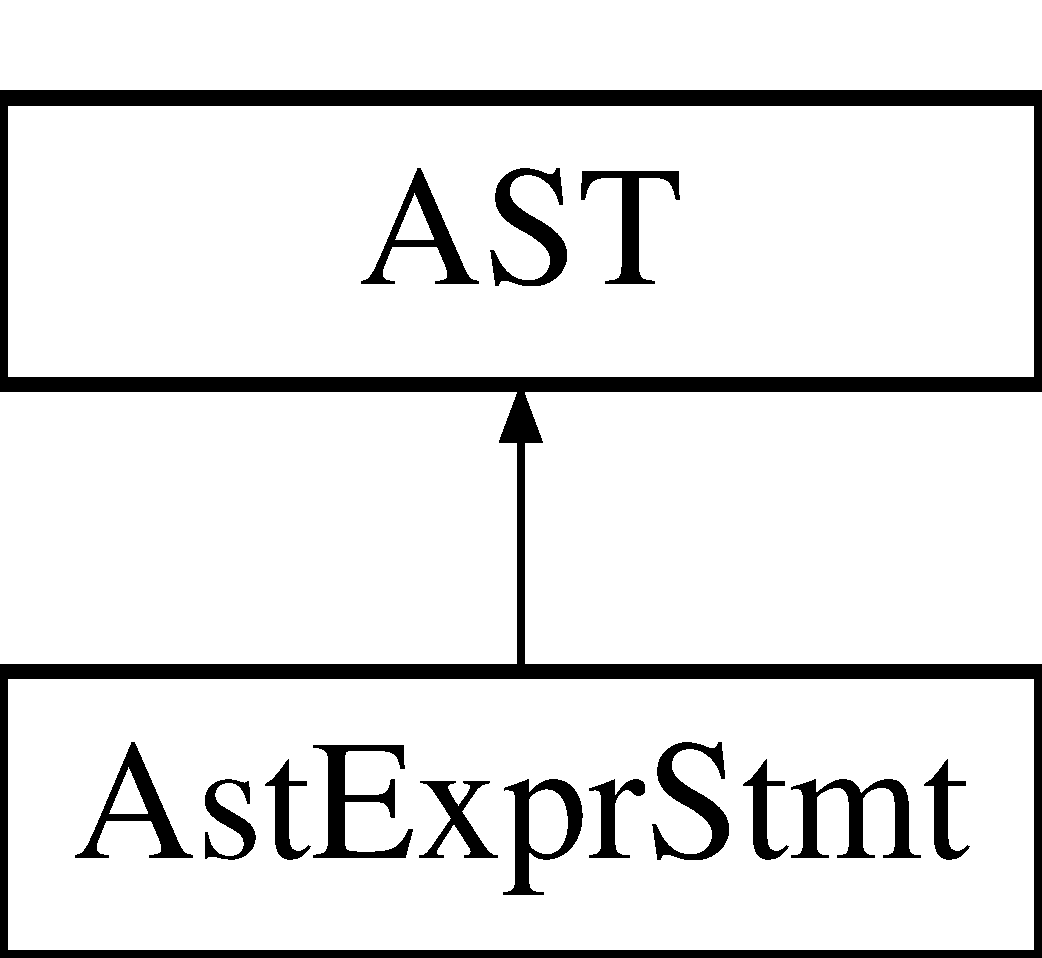
\includegraphics[height=2.000000cm]{classAstExprStmt}
\end{center}
\end{figure}
\subsection*{Public Member Functions}
\begin{DoxyCompactItemize}
\item 
\hypertarget{classAstExprStmt_a1ae9430bd6b1d01b6e3df6924012af56}{{\bfseries Ast\-Expr\-Stmt} (\hyperlink{classAstExpression}{Ast\-Expression} $\ast$e)}\label{classAstExprStmt_a1ae9430bd6b1d01b6e3df6924012af56}

\item 
void \hyperlink{classAstExprStmt_aa6763a98f7659d35edf7cf60557609b2}{Visit} ()
\begin{DoxyCompactList}\small\item\em This function is responsible for tree traversals. \end{DoxyCompactList}\item 
\hypertarget{classAstExprStmt_a1ae9430bd6b1d01b6e3df6924012af56}{{\bfseries Ast\-Expr\-Stmt} (\hyperlink{classAstExpression}{Ast\-Expression} $\ast$e)}\label{classAstExprStmt_a1ae9430bd6b1d01b6e3df6924012af56}

\item 
void \hyperlink{classAstExprStmt_aa6763a98f7659d35edf7cf60557609b2}{Visit} ()
\begin{DoxyCompactList}\small\item\em This function is responsible for tree traversals. \end{DoxyCompactList}\item 
\hypertarget{classAstExprStmt_a1ae9430bd6b1d01b6e3df6924012af56}{{\bfseries Ast\-Expr\-Stmt} (\hyperlink{classAstExpression}{Ast\-Expression} $\ast$e)}\label{classAstExprStmt_a1ae9430bd6b1d01b6e3df6924012af56}

\item 
void \hyperlink{classAstExprStmt_aa6763a98f7659d35edf7cf60557609b2}{Visit} ()
\begin{DoxyCompactList}\small\item\em This function is responsible for tree traversals. \end{DoxyCompactList}\item 
\hypertarget{classAstExprStmt_a1ae9430bd6b1d01b6e3df6924012af56}{{\bfseries Ast\-Expr\-Stmt} (\hyperlink{classAstExpression}{Ast\-Expression} $\ast$e)}\label{classAstExprStmt_a1ae9430bd6b1d01b6e3df6924012af56}

\item 
void \hyperlink{classAstExprStmt_aa6763a98f7659d35edf7cf60557609b2}{Visit} ()
\begin{DoxyCompactList}\small\item\em This function is responsible for tree traversals. \end{DoxyCompactList}\item 
void \hyperlink{classAST_a71d680856e95ff89f55d5311a552eba6}{set\-Label} (string l)
\begin{DoxyCompactList}\small\item\em Sets the label for the node. \end{DoxyCompactList}\item 
void \hyperlink{classAST_a71d680856e95ff89f55d5311a552eba6}{set\-Label} (string l)
\begin{DoxyCompactList}\small\item\em Sets the label for the node. \end{DoxyCompactList}\item 
void \hyperlink{classAST_a71d680856e95ff89f55d5311a552eba6}{set\-Label} (string l)
\begin{DoxyCompactList}\small\item\em Sets the label for the node. \end{DoxyCompactList}\item 
void \hyperlink{classAST_a71d680856e95ff89f55d5311a552eba6}{set\-Label} (string l)
\begin{DoxyCompactList}\small\item\em Sets the label for the node. \end{DoxyCompactList}\item 
int \hyperlink{classAST_ab7a5b1d9f1c2de0d98deb356f724a42c}{get\-U\-I\-D} ()
\begin{DoxyCompactList}\small\item\em Gets the node's unique I\-D. \end{DoxyCompactList}\item 
int \hyperlink{classAST_ab7a5b1d9f1c2de0d98deb356f724a42c}{get\-U\-I\-D} ()
\begin{DoxyCompactList}\small\item\em Gets the node's unique I\-D. \end{DoxyCompactList}\item 
int \hyperlink{classAST_ab7a5b1d9f1c2de0d98deb356f724a42c}{get\-U\-I\-D} ()
\begin{DoxyCompactList}\small\item\em Gets the node's unique I\-D. \end{DoxyCompactList}\item 
int \hyperlink{classAST_ab7a5b1d9f1c2de0d98deb356f724a42c}{get\-U\-I\-D} ()
\begin{DoxyCompactList}\small\item\em Gets the node's unique I\-D. \end{DoxyCompactList}\item 
string \hyperlink{classAST_aee029be902fffc927d16ccb03eb922ad}{get\-Label} ()
\begin{DoxyCompactList}\small\item\em Gets the node's label. \end{DoxyCompactList}\item 
string \hyperlink{classAST_aee029be902fffc927d16ccb03eb922ad}{get\-Label} ()
\begin{DoxyCompactList}\small\item\em Gets the node's label. \end{DoxyCompactList}\item 
string \hyperlink{classAST_aee029be902fffc927d16ccb03eb922ad}{get\-Label} ()
\begin{DoxyCompactList}\small\item\em Gets the node's label. \end{DoxyCompactList}\item 
string \hyperlink{classAST_aee029be902fffc927d16ccb03eb922ad}{get\-Label} ()
\begin{DoxyCompactList}\small\item\em Gets the node's label. \end{DoxyCompactList}\end{DoxyCompactItemize}
\subsection*{Public Attributes}
\begin{DoxyCompactItemize}
\item 
\hypertarget{classAST_aaf215802de409f8096c063d01ffa6783}{bool \hyperlink{classAST_aaf215802de409f8096c063d01ffa6783}{needs\-Cast}}\label{classAST_aaf215802de409f8096c063d01ffa6783}

\begin{DoxyCompactList}\small\item\em This indicates if cast 3\-A\-C needs to be output, and is only relevant for expressions. \end{DoxyCompactList}\item 
\hypertarget{classAST_afa9e77ef650ec6664458fa6cb55be985}{bool \hyperlink{classAST_afa9e77ef650ec6664458fa6cb55be985}{is\-Conv}}\label{classAST_afa9e77ef650ec6664458fa6cb55be985}

\begin{DoxyCompactList}\small\item\em Indicates is a conversion is possible. \end{DoxyCompactList}\item 
\hypertarget{classAST_a61ef3317e023d45237e06615b387cd6b}{C\-O\-N\-V\-E\-R\-S\-I\-O\-N\-T\-Y\-P\-E \hyperlink{classAST_a61ef3317e023d45237e06615b387cd6b}{conv\-Type}}\label{classAST_a61ef3317e023d45237e06615b387cd6b}

\begin{DoxyCompactList}\small\item\em If needs\-Cast is true, then this indicates what the cast should be. \end{DoxyCompactList}\item 
\hypertarget{classAST_aea9b07b39d24183f38c0029cec0a878e}{int \hyperlink{classAST_aea9b07b39d24183f38c0029cec0a878e}{operand\-To\-Cast}}\label{classAST_aea9b07b39d24183f38c0029cec0a878e}

\begin{DoxyCompactList}\small\item\em This indicates if the first or second operand should be the one that is cast. \end{DoxyCompactList}\end{DoxyCompactItemize}
\subsection*{Static Public Attributes}
\begin{DoxyCompactItemize}
\item 
\hypertarget{classAST_a5fdfd5f7b104dd92889163bdadbc68d6}{static \hyperlink{classVisualizer}{Visualizer} \hyperlink{classAST_a5fdfd5f7b104dd92889163bdadbc68d6}{vis}}\label{classAST_a5fdfd5f7b104dd92889163bdadbc68d6}

\begin{DoxyCompactList}\small\item\em Static visualizer instance for generating the visualization of the \hyperlink{classAST}{A\-S\-T}. \end{DoxyCompactList}\item 
\hypertarget{classAST_a8a3ace322f50e030331065d644ee55ee}{static \hyperlink{classTAC__Generator}{T\-A\-C\-\_\-\-Generator} \hyperlink{classAST_a8a3ace322f50e030331065d644ee55ee}{tac\-Gen}}\label{classAST_a8a3ace322f50e030331065d644ee55ee}

\begin{DoxyCompactList}\small\item\em Three address code generator. \end{DoxyCompactList}\item 
\hypertarget{classAST_a1f69448c6dc368d005631a128460083d}{static string {\bfseries current\-Temp} =\char`\"{}\char`\"{}}\label{classAST_a1f69448c6dc368d005631a128460083d}

\item 
\hypertarget{classAST_a551aec090c932ab69365238b40a8a4eb}{static string \hyperlink{classAST_a551aec090c932ab69365238b40a8a4eb}{return\-Label} =\char`\"{}\char`\"{}}\label{classAST_a551aec090c932ab69365238b40a8a4eb}

\begin{DoxyCompactList}\small\item\em This is for storing the string id of any temporary result register that may be created during 3\-A\-C generation. \end{DoxyCompactList}\item 
\hypertarget{classAST_a73c0a266df52be71e6b527b6aa635173}{static list$<$ string $>$ {\bfseries temp\-Stack}}\label{classAST_a73c0a266df52be71e6b527b6aa635173}

\item 
\hypertarget{classAST_abf9e84b541ff04b7bb64e6e4371512d4}{static string {\bfseries last\-I\-D} =\char`\"{}\char`\"{}}\label{classAST_abf9e84b541ff04b7bb64e6e4371512d4}

\item 
\hypertarget{classAST_a163003bfe9c30510ec8039870346049f}{static \hyperlink{classSymTab}{Sym\-Tab} $\ast$ {\bfseries symbol\-Table} =N\-U\-L\-L}\label{classAST_a163003bfe9c30510ec8039870346049f}

\item 
\hypertarget{classAST_a5c3cc894d9c0453523dec9ed76f18a04}{static string {\bfseries current\-Function} =\char`\"{}\char`\"{}}\label{classAST_a5c3cc894d9c0453523dec9ed76f18a04}

\item 
\hypertarget{classAST_a66155513b59ff1a04c8ece8b20ec31f5}{static int {\bfseries current\-Constant\-Value} =0}\label{classAST_a66155513b59ff1a04c8ece8b20ec31f5}

\item 
\hypertarget{classAST_a3d031d7bab635ba1f015aade5943f40c}{static string {\bfseries current\-Id\-Name} =\char`\"{}\char`\"{}}\label{classAST_a3d031d7bab635ba1f015aade5943f40c}

\item 
\hypertarget{classAST_a16c4b6e54febc1a26b31a64a46972ef0}{static int {\bfseries current\-Index\-Val} = 0}\label{classAST_a16c4b6e54febc1a26b31a64a46972ef0}

\item 
\hypertarget{classAST_a6fc65ae9dd064a88941d4b88669b19db}{static string {\bfseries current\-I\-D} = \char`\"{}\char`\"{}}\label{classAST_a6fc65ae9dd064a88941d4b88669b19db}

\end{DoxyCompactItemize}
\subsection*{Protected Attributes}
\begin{DoxyCompactItemize}
\item 
\hypertarget{classAST_a847b778f1c3dd5a19de32de432ee6e15}{int \hyperlink{classAST_a847b778f1c3dd5a19de32de432ee6e15}{uid}}\label{classAST_a847b778f1c3dd5a19de32de432ee6e15}

\begin{DoxyCompactList}\small\item\em The unique id. \end{DoxyCompactList}\item 
\hypertarget{classAST_ab2e239ccc0688d2341724432ff5a1a31}{string \hyperlink{classAST_ab2e239ccc0688d2341724432ff5a1a31}{label}}\label{classAST_ab2e239ccc0688d2341724432ff5a1a31}

\begin{DoxyCompactList}\small\item\em The label to be printed in the visualization. \end{DoxyCompactList}\end{DoxyCompactItemize}
\subsection*{Private Attributes}
\begin{DoxyCompactItemize}
\item 
\hypertarget{classAstExprStmt_a65a334737f1d579ff890c46ea4a91777}{\hyperlink{classAstExpression}{Ast\-Expression} $\ast$ {\bfseries expr}}\label{classAstExprStmt_a65a334737f1d579ff890c46ea4a91777}

\end{DoxyCompactItemize}


\subsection{Detailed Description}


Definition at line 947 of file Ast.\-h.



\subsection{Member Function Documentation}
\hypertarget{classAST_aee029be902fffc927d16ccb03eb922ad}{\index{Ast\-Expr\-Stmt@{Ast\-Expr\-Stmt}!get\-Label@{get\-Label}}
\index{get\-Label@{get\-Label}!AstExprStmt@{Ast\-Expr\-Stmt}}
\subsubsection[{get\-Label}]{\setlength{\rightskip}{0pt plus 5cm}string A\-S\-T\-::get\-Label (
\begin{DoxyParamCaption}
{}
\end{DoxyParamCaption}
)\hspace{0.3cm}{\ttfamily [inline]}, {\ttfamily [inherited]}}}\label{classAST_aee029be902fffc927d16ccb03eb922ad}


Gets the node's label. 

\begin{DoxyReturn}{Returns}
The label 
\end{DoxyReturn}


Definition at line 60 of file Ast.\-h.

\hypertarget{classAST_aee029be902fffc927d16ccb03eb922ad}{\index{Ast\-Expr\-Stmt@{Ast\-Expr\-Stmt}!get\-Label@{get\-Label}}
\index{get\-Label@{get\-Label}!AstExprStmt@{Ast\-Expr\-Stmt}}
\subsubsection[{get\-Label}]{\setlength{\rightskip}{0pt plus 5cm}string A\-S\-T\-::get\-Label (
\begin{DoxyParamCaption}
{}
\end{DoxyParamCaption}
)\hspace{0.3cm}{\ttfamily [inline]}, {\ttfamily [inherited]}}}\label{classAST_aee029be902fffc927d16ccb03eb922ad}


Gets the node's label. 

\begin{DoxyReturn}{Returns}
The label 
\end{DoxyReturn}


Definition at line 60 of file C\-Scanner.\-ll.

\hypertarget{classAST_aee029be902fffc927d16ccb03eb922ad}{\index{Ast\-Expr\-Stmt@{Ast\-Expr\-Stmt}!get\-Label@{get\-Label}}
\index{get\-Label@{get\-Label}!AstExprStmt@{Ast\-Expr\-Stmt}}
\subsubsection[{get\-Label}]{\setlength{\rightskip}{0pt plus 5cm}string A\-S\-T\-::get\-Label (
\begin{DoxyParamCaption}
{}
\end{DoxyParamCaption}
)\hspace{0.3cm}{\ttfamily [inline]}, {\ttfamily [inherited]}}}\label{classAST_aee029be902fffc927d16ccb03eb922ad}


Gets the node's label. 

\begin{DoxyReturn}{Returns}
The label 
\end{DoxyReturn}


Definition at line 60 of file C\-Parser.\-yy.

\hypertarget{classAST_aee029be902fffc927d16ccb03eb922ad}{\index{Ast\-Expr\-Stmt@{Ast\-Expr\-Stmt}!get\-Label@{get\-Label}}
\index{get\-Label@{get\-Label}!AstExprStmt@{Ast\-Expr\-Stmt}}
\subsubsection[{get\-Label}]{\setlength{\rightskip}{0pt plus 5cm}string A\-S\-T\-::get\-Label (
\begin{DoxyParamCaption}
{}
\end{DoxyParamCaption}
)\hspace{0.3cm}{\ttfamily [inline]}, {\ttfamily [inherited]}}}\label{classAST_aee029be902fffc927d16ccb03eb922ad}


Gets the node's label. 

\begin{DoxyReturn}{Returns}
The label 
\end{DoxyReturn}


Definition at line 60 of file C\-Parser.\-yy.

\hypertarget{classAST_ab7a5b1d9f1c2de0d98deb356f724a42c}{\index{Ast\-Expr\-Stmt@{Ast\-Expr\-Stmt}!get\-U\-I\-D@{get\-U\-I\-D}}
\index{get\-U\-I\-D@{get\-U\-I\-D}!AstExprStmt@{Ast\-Expr\-Stmt}}
\subsubsection[{get\-U\-I\-D}]{\setlength{\rightskip}{0pt plus 5cm}int A\-S\-T\-::get\-U\-I\-D (
\begin{DoxyParamCaption}
{}
\end{DoxyParamCaption}
)\hspace{0.3cm}{\ttfamily [inline]}, {\ttfamily [inherited]}}}\label{classAST_ab7a5b1d9f1c2de0d98deb356f724a42c}


Gets the node's unique I\-D. 

\begin{DoxyReturn}{Returns}
The unique id 
\end{DoxyReturn}


Definition at line 53 of file C\-Parser.\-yy.

\hypertarget{classAST_ab7a5b1d9f1c2de0d98deb356f724a42c}{\index{Ast\-Expr\-Stmt@{Ast\-Expr\-Stmt}!get\-U\-I\-D@{get\-U\-I\-D}}
\index{get\-U\-I\-D@{get\-U\-I\-D}!AstExprStmt@{Ast\-Expr\-Stmt}}
\subsubsection[{get\-U\-I\-D}]{\setlength{\rightskip}{0pt plus 5cm}int A\-S\-T\-::get\-U\-I\-D (
\begin{DoxyParamCaption}
{}
\end{DoxyParamCaption}
)\hspace{0.3cm}{\ttfamily [inline]}, {\ttfamily [inherited]}}}\label{classAST_ab7a5b1d9f1c2de0d98deb356f724a42c}


Gets the node's unique I\-D. 

\begin{DoxyReturn}{Returns}
The unique id 
\end{DoxyReturn}


Definition at line 53 of file C\-Parser.\-yy.

\hypertarget{classAST_ab7a5b1d9f1c2de0d98deb356f724a42c}{\index{Ast\-Expr\-Stmt@{Ast\-Expr\-Stmt}!get\-U\-I\-D@{get\-U\-I\-D}}
\index{get\-U\-I\-D@{get\-U\-I\-D}!AstExprStmt@{Ast\-Expr\-Stmt}}
\subsubsection[{get\-U\-I\-D}]{\setlength{\rightskip}{0pt plus 5cm}int A\-S\-T\-::get\-U\-I\-D (
\begin{DoxyParamCaption}
{}
\end{DoxyParamCaption}
)\hspace{0.3cm}{\ttfamily [inline]}, {\ttfamily [inherited]}}}\label{classAST_ab7a5b1d9f1c2de0d98deb356f724a42c}


Gets the node's unique I\-D. 

\begin{DoxyReturn}{Returns}
The unique id 
\end{DoxyReturn}


Definition at line 53 of file C\-Scanner.\-ll.

\hypertarget{classAST_ab7a5b1d9f1c2de0d98deb356f724a42c}{\index{Ast\-Expr\-Stmt@{Ast\-Expr\-Stmt}!get\-U\-I\-D@{get\-U\-I\-D}}
\index{get\-U\-I\-D@{get\-U\-I\-D}!AstExprStmt@{Ast\-Expr\-Stmt}}
\subsubsection[{get\-U\-I\-D}]{\setlength{\rightskip}{0pt plus 5cm}int A\-S\-T\-::get\-U\-I\-D (
\begin{DoxyParamCaption}
{}
\end{DoxyParamCaption}
)\hspace{0.3cm}{\ttfamily [inline]}, {\ttfamily [inherited]}}}\label{classAST_ab7a5b1d9f1c2de0d98deb356f724a42c}


Gets the node's unique I\-D. 

\begin{DoxyReturn}{Returns}
The unique id 
\end{DoxyReturn}


Definition at line 53 of file Ast.\-h.

\hypertarget{classAST_a71d680856e95ff89f55d5311a552eba6}{\index{Ast\-Expr\-Stmt@{Ast\-Expr\-Stmt}!set\-Label@{set\-Label}}
\index{set\-Label@{set\-Label}!AstExprStmt@{Ast\-Expr\-Stmt}}
\subsubsection[{set\-Label}]{\setlength{\rightskip}{0pt plus 5cm}void A\-S\-T\-::set\-Label (
\begin{DoxyParamCaption}
\item[{string}]{l}
\end{DoxyParamCaption}
)\hspace{0.3cm}{\ttfamily [inline]}, {\ttfamily [inherited]}}}\label{classAST_a71d680856e95ff89f55d5311a552eba6}


Sets the label for the node. 


\begin{DoxyParams}{Parameters}
{\em l} & The label string \\
\hline
\end{DoxyParams}


Definition at line 43 of file C\-Scanner.\-ll.

\hypertarget{classAST_a71d680856e95ff89f55d5311a552eba6}{\index{Ast\-Expr\-Stmt@{Ast\-Expr\-Stmt}!set\-Label@{set\-Label}}
\index{set\-Label@{set\-Label}!AstExprStmt@{Ast\-Expr\-Stmt}}
\subsubsection[{set\-Label}]{\setlength{\rightskip}{0pt plus 5cm}void A\-S\-T\-::set\-Label (
\begin{DoxyParamCaption}
\item[{string}]{l}
\end{DoxyParamCaption}
)\hspace{0.3cm}{\ttfamily [inline]}, {\ttfamily [inherited]}}}\label{classAST_a71d680856e95ff89f55d5311a552eba6}


Sets the label for the node. 


\begin{DoxyParams}{Parameters}
{\em l} & The label string \\
\hline
\end{DoxyParams}


Definition at line 43 of file C\-Parser.\-yy.

\hypertarget{classAST_a71d680856e95ff89f55d5311a552eba6}{\index{Ast\-Expr\-Stmt@{Ast\-Expr\-Stmt}!set\-Label@{set\-Label}}
\index{set\-Label@{set\-Label}!AstExprStmt@{Ast\-Expr\-Stmt}}
\subsubsection[{set\-Label}]{\setlength{\rightskip}{0pt plus 5cm}void A\-S\-T\-::set\-Label (
\begin{DoxyParamCaption}
\item[{string}]{l}
\end{DoxyParamCaption}
)\hspace{0.3cm}{\ttfamily [inline]}, {\ttfamily [inherited]}}}\label{classAST_a71d680856e95ff89f55d5311a552eba6}


Sets the label for the node. 


\begin{DoxyParams}{Parameters}
{\em l} & The label string \\
\hline
\end{DoxyParams}


Definition at line 43 of file Ast.\-h.

\hypertarget{classAST_a71d680856e95ff89f55d5311a552eba6}{\index{Ast\-Expr\-Stmt@{Ast\-Expr\-Stmt}!set\-Label@{set\-Label}}
\index{set\-Label@{set\-Label}!AstExprStmt@{Ast\-Expr\-Stmt}}
\subsubsection[{set\-Label}]{\setlength{\rightskip}{0pt plus 5cm}void A\-S\-T\-::set\-Label (
\begin{DoxyParamCaption}
\item[{string}]{l}
\end{DoxyParamCaption}
)\hspace{0.3cm}{\ttfamily [inline]}, {\ttfamily [inherited]}}}\label{classAST_a71d680856e95ff89f55d5311a552eba6}


Sets the label for the node. 


\begin{DoxyParams}{Parameters}
{\em l} & The label string \\
\hline
\end{DoxyParams}


Definition at line 43 of file C\-Parser.\-yy.

\hypertarget{classAstExprStmt_aa6763a98f7659d35edf7cf60557609b2}{\index{Ast\-Expr\-Stmt@{Ast\-Expr\-Stmt}!Visit@{Visit}}
\index{Visit@{Visit}!AstExprStmt@{Ast\-Expr\-Stmt}}
\subsubsection[{Visit}]{\setlength{\rightskip}{0pt plus 5cm}void Ast\-Expr\-Stmt\-::\-Visit (
\begin{DoxyParamCaption}
{}
\end{DoxyParamCaption}
)\hspace{0.3cm}{\ttfamily [virtual]}}}\label{classAstExprStmt_aa6763a98f7659d35edf7cf60557609b2}


This function is responsible for tree traversals. 

This function will call the Visit functions of each of it's children nodes, call the visualization code for itself, and output any 3\-A\-C that can be generated at the current node. 

Reimplemented from \hyperlink{classAST_a5828cc86f2c4f1a0aeab6d7069e8fd82}{A\-S\-T}.



Definition at line 2714 of file Ast.\-cpp.

\hypertarget{classAstExprStmt_aa6763a98f7659d35edf7cf60557609b2}{\index{Ast\-Expr\-Stmt@{Ast\-Expr\-Stmt}!Visit@{Visit}}
\index{Visit@{Visit}!AstExprStmt@{Ast\-Expr\-Stmt}}
\subsubsection[{Visit}]{\setlength{\rightskip}{0pt plus 5cm}void Ast\-Expr\-Stmt\-::\-Visit (
\begin{DoxyParamCaption}
{}
\end{DoxyParamCaption}
)\hspace{0.3cm}{\ttfamily [virtual]}}}\label{classAstExprStmt_aa6763a98f7659d35edf7cf60557609b2}


This function is responsible for tree traversals. 

This function will call the Visit functions of each of it's children nodes, call the visualization code for itself, and output any 3\-A\-C that can be generated at the current node. 

Reimplemented from \hyperlink{classAST_a5828cc86f2c4f1a0aeab6d7069e8fd82}{A\-S\-T}.

\hypertarget{classAstExprStmt_aa6763a98f7659d35edf7cf60557609b2}{\index{Ast\-Expr\-Stmt@{Ast\-Expr\-Stmt}!Visit@{Visit}}
\index{Visit@{Visit}!AstExprStmt@{Ast\-Expr\-Stmt}}
\subsubsection[{Visit}]{\setlength{\rightskip}{0pt plus 5cm}void Ast\-Expr\-Stmt\-::\-Visit (
\begin{DoxyParamCaption}
{}
\end{DoxyParamCaption}
)\hspace{0.3cm}{\ttfamily [virtual]}}}\label{classAstExprStmt_aa6763a98f7659d35edf7cf60557609b2}


This function is responsible for tree traversals. 

This function will call the Visit functions of each of it's children nodes, call the visualization code for itself, and output any 3\-A\-C that can be generated at the current node. 

Reimplemented from \hyperlink{classAST_a5828cc86f2c4f1a0aeab6d7069e8fd82}{A\-S\-T}.

\hypertarget{classAstExprStmt_aa6763a98f7659d35edf7cf60557609b2}{\index{Ast\-Expr\-Stmt@{Ast\-Expr\-Stmt}!Visit@{Visit}}
\index{Visit@{Visit}!AstExprStmt@{Ast\-Expr\-Stmt}}
\subsubsection[{Visit}]{\setlength{\rightskip}{0pt plus 5cm}void Ast\-Expr\-Stmt\-::\-Visit (
\begin{DoxyParamCaption}
{}
\end{DoxyParamCaption}
)\hspace{0.3cm}{\ttfamily [virtual]}}}\label{classAstExprStmt_aa6763a98f7659d35edf7cf60557609b2}


This function is responsible for tree traversals. 

This function will call the Visit functions of each of it's children nodes, call the visualization code for itself, and output any 3\-A\-C that can be generated at the current node. 

Reimplemented from \hyperlink{classAST_a5828cc86f2c4f1a0aeab6d7069e8fd82}{A\-S\-T}.



The documentation for this class was generated from the following files\-:\begin{DoxyCompactItemize}
\item 
Ast.\-h\item 
Ast.\-cpp\end{DoxyCompactItemize}

\hypertarget{classAstFor}{\section{Ast\-For Class Reference}
\label{classAstFor}\index{Ast\-For@{Ast\-For}}
}
Inheritance diagram for Ast\-For\-:\begin{figure}[H]
\begin{center}
\leavevmode
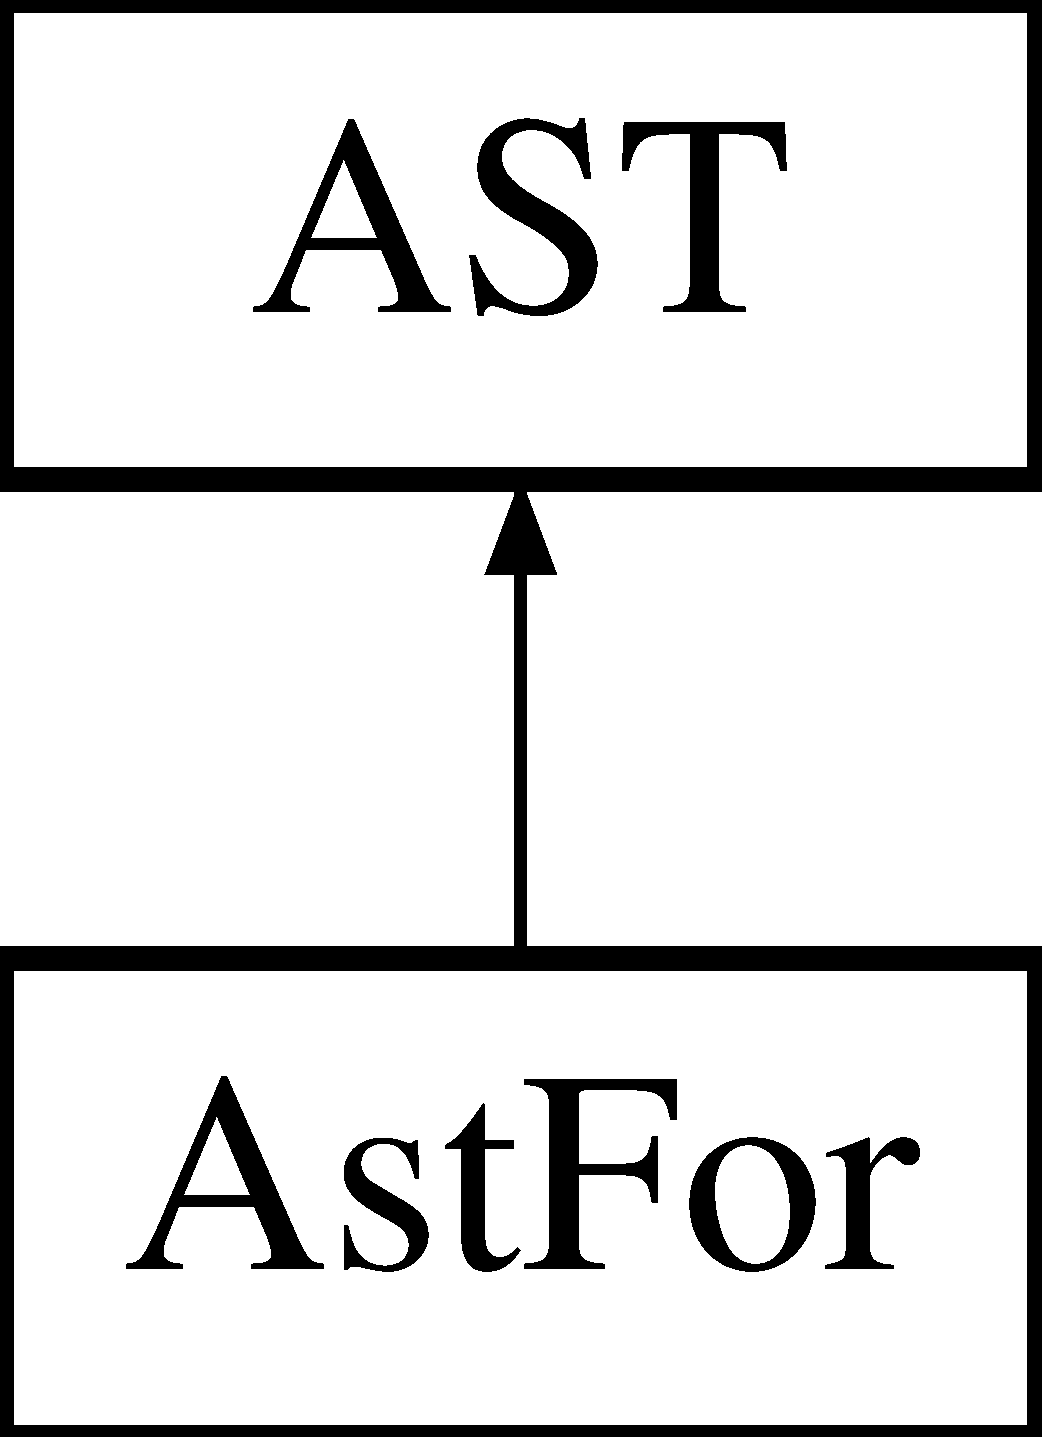
\includegraphics[height=2.000000cm]{classAstFor}
\end{center}
\end{figure}
\subsection*{Public Member Functions}
\begin{DoxyCompactItemize}
\item 
\hypertarget{classAstFor_af4b510c833d8cb2b64e5ba1d700b6e1b}{{\bfseries Ast\-For} (\hyperlink{classAstExpression}{Ast\-Expression} $\ast$init, \hyperlink{classAstExpression}{Ast\-Expression} $\ast$test, \hyperlink{classAstExpression}{Ast\-Expression} $\ast$increment, \hyperlink{classAstStatement}{Ast\-Statement} $\ast$statement)}\label{classAstFor_af4b510c833d8cb2b64e5ba1d700b6e1b}

\item 
void \hyperlink{classAstFor_aabb94ea30de2b634b35c02ec3688d0ff}{Visit} ()
\begin{DoxyCompactList}\small\item\em This function is responsible for tree traversals. \end{DoxyCompactList}\item 
\hypertarget{classAstFor_af4b510c833d8cb2b64e5ba1d700b6e1b}{{\bfseries Ast\-For} (\hyperlink{classAstExpression}{Ast\-Expression} $\ast$init, \hyperlink{classAstExpression}{Ast\-Expression} $\ast$test, \hyperlink{classAstExpression}{Ast\-Expression} $\ast$increment, \hyperlink{classAstStatement}{Ast\-Statement} $\ast$statement)}\label{classAstFor_af4b510c833d8cb2b64e5ba1d700b6e1b}

\item 
void \hyperlink{classAstFor_aabb94ea30de2b634b35c02ec3688d0ff}{Visit} ()
\begin{DoxyCompactList}\small\item\em This function is responsible for tree traversals. \end{DoxyCompactList}\item 
\hypertarget{classAstFor_af4b510c833d8cb2b64e5ba1d700b6e1b}{{\bfseries Ast\-For} (\hyperlink{classAstExpression}{Ast\-Expression} $\ast$init, \hyperlink{classAstExpression}{Ast\-Expression} $\ast$test, \hyperlink{classAstExpression}{Ast\-Expression} $\ast$increment, \hyperlink{classAstStatement}{Ast\-Statement} $\ast$statement)}\label{classAstFor_af4b510c833d8cb2b64e5ba1d700b6e1b}

\item 
void \hyperlink{classAstFor_aabb94ea30de2b634b35c02ec3688d0ff}{Visit} ()
\begin{DoxyCompactList}\small\item\em This function is responsible for tree traversals. \end{DoxyCompactList}\item 
\hypertarget{classAstFor_af4b510c833d8cb2b64e5ba1d700b6e1b}{{\bfseries Ast\-For} (\hyperlink{classAstExpression}{Ast\-Expression} $\ast$init, \hyperlink{classAstExpression}{Ast\-Expression} $\ast$test, \hyperlink{classAstExpression}{Ast\-Expression} $\ast$increment, \hyperlink{classAstStatement}{Ast\-Statement} $\ast$statement)}\label{classAstFor_af4b510c833d8cb2b64e5ba1d700b6e1b}

\item 
void \hyperlink{classAstFor_aabb94ea30de2b634b35c02ec3688d0ff}{Visit} ()
\begin{DoxyCompactList}\small\item\em This function is responsible for tree traversals. \end{DoxyCompactList}\item 
void \hyperlink{classAST_a71d680856e95ff89f55d5311a552eba6}{set\-Label} (string l)
\begin{DoxyCompactList}\small\item\em Sets the label for the node. \end{DoxyCompactList}\item 
void \hyperlink{classAST_a71d680856e95ff89f55d5311a552eba6}{set\-Label} (string l)
\begin{DoxyCompactList}\small\item\em Sets the label for the node. \end{DoxyCompactList}\item 
void \hyperlink{classAST_a71d680856e95ff89f55d5311a552eba6}{set\-Label} (string l)
\begin{DoxyCompactList}\small\item\em Sets the label for the node. \end{DoxyCompactList}\item 
void \hyperlink{classAST_a71d680856e95ff89f55d5311a552eba6}{set\-Label} (string l)
\begin{DoxyCompactList}\small\item\em Sets the label for the node. \end{DoxyCompactList}\item 
int \hyperlink{classAST_ab7a5b1d9f1c2de0d98deb356f724a42c}{get\-U\-I\-D} ()
\begin{DoxyCompactList}\small\item\em Gets the node's unique I\-D. \end{DoxyCompactList}\item 
int \hyperlink{classAST_ab7a5b1d9f1c2de0d98deb356f724a42c}{get\-U\-I\-D} ()
\begin{DoxyCompactList}\small\item\em Gets the node's unique I\-D. \end{DoxyCompactList}\item 
int \hyperlink{classAST_ab7a5b1d9f1c2de0d98deb356f724a42c}{get\-U\-I\-D} ()
\begin{DoxyCompactList}\small\item\em Gets the node's unique I\-D. \end{DoxyCompactList}\item 
int \hyperlink{classAST_ab7a5b1d9f1c2de0d98deb356f724a42c}{get\-U\-I\-D} ()
\begin{DoxyCompactList}\small\item\em Gets the node's unique I\-D. \end{DoxyCompactList}\item 
string \hyperlink{classAST_aee029be902fffc927d16ccb03eb922ad}{get\-Label} ()
\begin{DoxyCompactList}\small\item\em Gets the node's label. \end{DoxyCompactList}\item 
string \hyperlink{classAST_aee029be902fffc927d16ccb03eb922ad}{get\-Label} ()
\begin{DoxyCompactList}\small\item\em Gets the node's label. \end{DoxyCompactList}\item 
string \hyperlink{classAST_aee029be902fffc927d16ccb03eb922ad}{get\-Label} ()
\begin{DoxyCompactList}\small\item\em Gets the node's label. \end{DoxyCompactList}\item 
string \hyperlink{classAST_aee029be902fffc927d16ccb03eb922ad}{get\-Label} ()
\begin{DoxyCompactList}\small\item\em Gets the node's label. \end{DoxyCompactList}\end{DoxyCompactItemize}
\subsection*{Public Attributes}
\begin{DoxyCompactItemize}
\item 
\hypertarget{classAST_aaf215802de409f8096c063d01ffa6783}{bool \hyperlink{classAST_aaf215802de409f8096c063d01ffa6783}{needs\-Cast}}\label{classAST_aaf215802de409f8096c063d01ffa6783}

\begin{DoxyCompactList}\small\item\em This indicates if cast 3\-A\-C needs to be output, and is only relevant for expressions. \end{DoxyCompactList}\item 
\hypertarget{classAST_afa9e77ef650ec6664458fa6cb55be985}{bool \hyperlink{classAST_afa9e77ef650ec6664458fa6cb55be985}{is\-Conv}}\label{classAST_afa9e77ef650ec6664458fa6cb55be985}

\begin{DoxyCompactList}\small\item\em Indicates is a conversion is possible. \end{DoxyCompactList}\item 
\hypertarget{classAST_a61ef3317e023d45237e06615b387cd6b}{C\-O\-N\-V\-E\-R\-S\-I\-O\-N\-T\-Y\-P\-E \hyperlink{classAST_a61ef3317e023d45237e06615b387cd6b}{conv\-Type}}\label{classAST_a61ef3317e023d45237e06615b387cd6b}

\begin{DoxyCompactList}\small\item\em If needs\-Cast is true, then this indicates what the cast should be. \end{DoxyCompactList}\item 
\hypertarget{classAST_aea9b07b39d24183f38c0029cec0a878e}{int \hyperlink{classAST_aea9b07b39d24183f38c0029cec0a878e}{operand\-To\-Cast}}\label{classAST_aea9b07b39d24183f38c0029cec0a878e}

\begin{DoxyCompactList}\small\item\em This indicates if the first or second operand should be the one that is cast. \end{DoxyCompactList}\end{DoxyCompactItemize}
\subsection*{Static Public Attributes}
\begin{DoxyCompactItemize}
\item 
\hypertarget{classAST_a5fdfd5f7b104dd92889163bdadbc68d6}{static \hyperlink{classVisualizer}{Visualizer} \hyperlink{classAST_a5fdfd5f7b104dd92889163bdadbc68d6}{vis}}\label{classAST_a5fdfd5f7b104dd92889163bdadbc68d6}

\begin{DoxyCompactList}\small\item\em Static visualizer instance for generating the visualization of the \hyperlink{classAST}{A\-S\-T}. \end{DoxyCompactList}\item 
\hypertarget{classAST_a8a3ace322f50e030331065d644ee55ee}{static \hyperlink{classTAC__Generator}{T\-A\-C\-\_\-\-Generator} \hyperlink{classAST_a8a3ace322f50e030331065d644ee55ee}{tac\-Gen}}\label{classAST_a8a3ace322f50e030331065d644ee55ee}

\begin{DoxyCompactList}\small\item\em Three address code generator. \end{DoxyCompactList}\item 
\hypertarget{classAST_a1f69448c6dc368d005631a128460083d}{static string {\bfseries current\-Temp} =\char`\"{}\char`\"{}}\label{classAST_a1f69448c6dc368d005631a128460083d}

\item 
\hypertarget{classAST_a551aec090c932ab69365238b40a8a4eb}{static string \hyperlink{classAST_a551aec090c932ab69365238b40a8a4eb}{return\-Label} =\char`\"{}\char`\"{}}\label{classAST_a551aec090c932ab69365238b40a8a4eb}

\begin{DoxyCompactList}\small\item\em This is for storing the string id of any temporary result register that may be created during 3\-A\-C generation. \end{DoxyCompactList}\item 
\hypertarget{classAST_a73c0a266df52be71e6b527b6aa635173}{static list$<$ string $>$ {\bfseries temp\-Stack}}\label{classAST_a73c0a266df52be71e6b527b6aa635173}

\item 
\hypertarget{classAST_abf9e84b541ff04b7bb64e6e4371512d4}{static string {\bfseries last\-I\-D} =\char`\"{}\char`\"{}}\label{classAST_abf9e84b541ff04b7bb64e6e4371512d4}

\item 
\hypertarget{classAST_a163003bfe9c30510ec8039870346049f}{static \hyperlink{classSymTab}{Sym\-Tab} $\ast$ {\bfseries symbol\-Table} =N\-U\-L\-L}\label{classAST_a163003bfe9c30510ec8039870346049f}

\item 
\hypertarget{classAST_a5c3cc894d9c0453523dec9ed76f18a04}{static string {\bfseries current\-Function} =\char`\"{}\char`\"{}}\label{classAST_a5c3cc894d9c0453523dec9ed76f18a04}

\item 
\hypertarget{classAST_a66155513b59ff1a04c8ece8b20ec31f5}{static int {\bfseries current\-Constant\-Value} =0}\label{classAST_a66155513b59ff1a04c8ece8b20ec31f5}

\item 
\hypertarget{classAST_a3d031d7bab635ba1f015aade5943f40c}{static string {\bfseries current\-Id\-Name} =\char`\"{}\char`\"{}}\label{classAST_a3d031d7bab635ba1f015aade5943f40c}

\item 
\hypertarget{classAST_a16c4b6e54febc1a26b31a64a46972ef0}{static int {\bfseries current\-Index\-Val} = 0}\label{classAST_a16c4b6e54febc1a26b31a64a46972ef0}

\item 
\hypertarget{classAST_a6fc65ae9dd064a88941d4b88669b19db}{static string {\bfseries current\-I\-D} = \char`\"{}\char`\"{}}\label{classAST_a6fc65ae9dd064a88941d4b88669b19db}

\end{DoxyCompactItemize}
\subsection*{Protected Attributes}
\begin{DoxyCompactItemize}
\item 
\hypertarget{classAST_a847b778f1c3dd5a19de32de432ee6e15}{int \hyperlink{classAST_a847b778f1c3dd5a19de32de432ee6e15}{uid}}\label{classAST_a847b778f1c3dd5a19de32de432ee6e15}

\begin{DoxyCompactList}\small\item\em The unique id. \end{DoxyCompactList}\item 
\hypertarget{classAST_ab2e239ccc0688d2341724432ff5a1a31}{string \hyperlink{classAST_ab2e239ccc0688d2341724432ff5a1a31}{label}}\label{classAST_ab2e239ccc0688d2341724432ff5a1a31}

\begin{DoxyCompactList}\small\item\em The label to be printed in the visualization. \end{DoxyCompactList}\end{DoxyCompactItemize}
\subsection*{Private Attributes}
\begin{DoxyCompactItemize}
\item 
\hypertarget{classAstFor_a8b1db1731d6d167759194f1e1fe7e184}{\hyperlink{classAstExpression}{Ast\-Expression} $\ast$ {\bfseries init}}\label{classAstFor_a8b1db1731d6d167759194f1e1fe7e184}

\item 
\hypertarget{classAstFor_afdac5e38cfb38a1c38363cce4eddc89d}{\hyperlink{classAstExpression}{Ast\-Expression} $\ast$ {\bfseries test}}\label{classAstFor_afdac5e38cfb38a1c38363cce4eddc89d}

\item 
\hypertarget{classAstFor_ab7c1bc4c1468434361857a43c519e33b}{\hyperlink{classAstExpression}{Ast\-Expression} $\ast$ {\bfseries increment}}\label{classAstFor_ab7c1bc4c1468434361857a43c519e33b}

\item 
\hypertarget{classAstFor_af451e2baf1679f41ff5680fc39b757d4}{\hyperlink{classAstStatement}{Ast\-Statement} $\ast$ {\bfseries statement}}\label{classAstFor_af451e2baf1679f41ff5680fc39b757d4}

\end{DoxyCompactItemize}


\subsection{Detailed Description}


Definition at line 864 of file Ast.\-h.



\subsection{Member Function Documentation}
\hypertarget{classAST_aee029be902fffc927d16ccb03eb922ad}{\index{Ast\-For@{Ast\-For}!get\-Label@{get\-Label}}
\index{get\-Label@{get\-Label}!AstFor@{Ast\-For}}
\subsubsection[{get\-Label}]{\setlength{\rightskip}{0pt plus 5cm}string A\-S\-T\-::get\-Label (
\begin{DoxyParamCaption}
{}
\end{DoxyParamCaption}
)\hspace{0.3cm}{\ttfamily [inline]}, {\ttfamily [inherited]}}}\label{classAST_aee029be902fffc927d16ccb03eb922ad}


Gets the node's label. 

\begin{DoxyReturn}{Returns}
The label 
\end{DoxyReturn}


Definition at line 60 of file Ast.\-h.

\hypertarget{classAST_aee029be902fffc927d16ccb03eb922ad}{\index{Ast\-For@{Ast\-For}!get\-Label@{get\-Label}}
\index{get\-Label@{get\-Label}!AstFor@{Ast\-For}}
\subsubsection[{get\-Label}]{\setlength{\rightskip}{0pt plus 5cm}string A\-S\-T\-::get\-Label (
\begin{DoxyParamCaption}
{}
\end{DoxyParamCaption}
)\hspace{0.3cm}{\ttfamily [inline]}, {\ttfamily [inherited]}}}\label{classAST_aee029be902fffc927d16ccb03eb922ad}


Gets the node's label. 

\begin{DoxyReturn}{Returns}
The label 
\end{DoxyReturn}


Definition at line 60 of file C\-Scanner.\-ll.

\hypertarget{classAST_aee029be902fffc927d16ccb03eb922ad}{\index{Ast\-For@{Ast\-For}!get\-Label@{get\-Label}}
\index{get\-Label@{get\-Label}!AstFor@{Ast\-For}}
\subsubsection[{get\-Label}]{\setlength{\rightskip}{0pt plus 5cm}string A\-S\-T\-::get\-Label (
\begin{DoxyParamCaption}
{}
\end{DoxyParamCaption}
)\hspace{0.3cm}{\ttfamily [inline]}, {\ttfamily [inherited]}}}\label{classAST_aee029be902fffc927d16ccb03eb922ad}


Gets the node's label. 

\begin{DoxyReturn}{Returns}
The label 
\end{DoxyReturn}


Definition at line 60 of file C\-Parser.\-yy.

\hypertarget{classAST_aee029be902fffc927d16ccb03eb922ad}{\index{Ast\-For@{Ast\-For}!get\-Label@{get\-Label}}
\index{get\-Label@{get\-Label}!AstFor@{Ast\-For}}
\subsubsection[{get\-Label}]{\setlength{\rightskip}{0pt plus 5cm}string A\-S\-T\-::get\-Label (
\begin{DoxyParamCaption}
{}
\end{DoxyParamCaption}
)\hspace{0.3cm}{\ttfamily [inline]}, {\ttfamily [inherited]}}}\label{classAST_aee029be902fffc927d16ccb03eb922ad}


Gets the node's label. 

\begin{DoxyReturn}{Returns}
The label 
\end{DoxyReturn}


Definition at line 60 of file C\-Parser.\-yy.

\hypertarget{classAST_ab7a5b1d9f1c2de0d98deb356f724a42c}{\index{Ast\-For@{Ast\-For}!get\-U\-I\-D@{get\-U\-I\-D}}
\index{get\-U\-I\-D@{get\-U\-I\-D}!AstFor@{Ast\-For}}
\subsubsection[{get\-U\-I\-D}]{\setlength{\rightskip}{0pt plus 5cm}int A\-S\-T\-::get\-U\-I\-D (
\begin{DoxyParamCaption}
{}
\end{DoxyParamCaption}
)\hspace{0.3cm}{\ttfamily [inline]}, {\ttfamily [inherited]}}}\label{classAST_ab7a5b1d9f1c2de0d98deb356f724a42c}


Gets the node's unique I\-D. 

\begin{DoxyReturn}{Returns}
The unique id 
\end{DoxyReturn}


Definition at line 53 of file C\-Parser.\-yy.

\hypertarget{classAST_ab7a5b1d9f1c2de0d98deb356f724a42c}{\index{Ast\-For@{Ast\-For}!get\-U\-I\-D@{get\-U\-I\-D}}
\index{get\-U\-I\-D@{get\-U\-I\-D}!AstFor@{Ast\-For}}
\subsubsection[{get\-U\-I\-D}]{\setlength{\rightskip}{0pt plus 5cm}int A\-S\-T\-::get\-U\-I\-D (
\begin{DoxyParamCaption}
{}
\end{DoxyParamCaption}
)\hspace{0.3cm}{\ttfamily [inline]}, {\ttfamily [inherited]}}}\label{classAST_ab7a5b1d9f1c2de0d98deb356f724a42c}


Gets the node's unique I\-D. 

\begin{DoxyReturn}{Returns}
The unique id 
\end{DoxyReturn}


Definition at line 53 of file C\-Parser.\-yy.

\hypertarget{classAST_ab7a5b1d9f1c2de0d98deb356f724a42c}{\index{Ast\-For@{Ast\-For}!get\-U\-I\-D@{get\-U\-I\-D}}
\index{get\-U\-I\-D@{get\-U\-I\-D}!AstFor@{Ast\-For}}
\subsubsection[{get\-U\-I\-D}]{\setlength{\rightskip}{0pt plus 5cm}int A\-S\-T\-::get\-U\-I\-D (
\begin{DoxyParamCaption}
{}
\end{DoxyParamCaption}
)\hspace{0.3cm}{\ttfamily [inline]}, {\ttfamily [inherited]}}}\label{classAST_ab7a5b1d9f1c2de0d98deb356f724a42c}


Gets the node's unique I\-D. 

\begin{DoxyReturn}{Returns}
The unique id 
\end{DoxyReturn}


Definition at line 53 of file C\-Scanner.\-ll.

\hypertarget{classAST_ab7a5b1d9f1c2de0d98deb356f724a42c}{\index{Ast\-For@{Ast\-For}!get\-U\-I\-D@{get\-U\-I\-D}}
\index{get\-U\-I\-D@{get\-U\-I\-D}!AstFor@{Ast\-For}}
\subsubsection[{get\-U\-I\-D}]{\setlength{\rightskip}{0pt plus 5cm}int A\-S\-T\-::get\-U\-I\-D (
\begin{DoxyParamCaption}
{}
\end{DoxyParamCaption}
)\hspace{0.3cm}{\ttfamily [inline]}, {\ttfamily [inherited]}}}\label{classAST_ab7a5b1d9f1c2de0d98deb356f724a42c}


Gets the node's unique I\-D. 

\begin{DoxyReturn}{Returns}
The unique id 
\end{DoxyReturn}


Definition at line 53 of file Ast.\-h.

\hypertarget{classAST_a71d680856e95ff89f55d5311a552eba6}{\index{Ast\-For@{Ast\-For}!set\-Label@{set\-Label}}
\index{set\-Label@{set\-Label}!AstFor@{Ast\-For}}
\subsubsection[{set\-Label}]{\setlength{\rightskip}{0pt plus 5cm}void A\-S\-T\-::set\-Label (
\begin{DoxyParamCaption}
\item[{string}]{l}
\end{DoxyParamCaption}
)\hspace{0.3cm}{\ttfamily [inline]}, {\ttfamily [inherited]}}}\label{classAST_a71d680856e95ff89f55d5311a552eba6}


Sets the label for the node. 


\begin{DoxyParams}{Parameters}
{\em l} & The label string \\
\hline
\end{DoxyParams}


Definition at line 43 of file C\-Scanner.\-ll.

\hypertarget{classAST_a71d680856e95ff89f55d5311a552eba6}{\index{Ast\-For@{Ast\-For}!set\-Label@{set\-Label}}
\index{set\-Label@{set\-Label}!AstFor@{Ast\-For}}
\subsubsection[{set\-Label}]{\setlength{\rightskip}{0pt plus 5cm}void A\-S\-T\-::set\-Label (
\begin{DoxyParamCaption}
\item[{string}]{l}
\end{DoxyParamCaption}
)\hspace{0.3cm}{\ttfamily [inline]}, {\ttfamily [inherited]}}}\label{classAST_a71d680856e95ff89f55d5311a552eba6}


Sets the label for the node. 


\begin{DoxyParams}{Parameters}
{\em l} & The label string \\
\hline
\end{DoxyParams}


Definition at line 43 of file C\-Parser.\-yy.

\hypertarget{classAST_a71d680856e95ff89f55d5311a552eba6}{\index{Ast\-For@{Ast\-For}!set\-Label@{set\-Label}}
\index{set\-Label@{set\-Label}!AstFor@{Ast\-For}}
\subsubsection[{set\-Label}]{\setlength{\rightskip}{0pt plus 5cm}void A\-S\-T\-::set\-Label (
\begin{DoxyParamCaption}
\item[{string}]{l}
\end{DoxyParamCaption}
)\hspace{0.3cm}{\ttfamily [inline]}, {\ttfamily [inherited]}}}\label{classAST_a71d680856e95ff89f55d5311a552eba6}


Sets the label for the node. 


\begin{DoxyParams}{Parameters}
{\em l} & The label string \\
\hline
\end{DoxyParams}


Definition at line 43 of file Ast.\-h.

\hypertarget{classAST_a71d680856e95ff89f55d5311a552eba6}{\index{Ast\-For@{Ast\-For}!set\-Label@{set\-Label}}
\index{set\-Label@{set\-Label}!AstFor@{Ast\-For}}
\subsubsection[{set\-Label}]{\setlength{\rightskip}{0pt plus 5cm}void A\-S\-T\-::set\-Label (
\begin{DoxyParamCaption}
\item[{string}]{l}
\end{DoxyParamCaption}
)\hspace{0.3cm}{\ttfamily [inline]}, {\ttfamily [inherited]}}}\label{classAST_a71d680856e95ff89f55d5311a552eba6}


Sets the label for the node. 


\begin{DoxyParams}{Parameters}
{\em l} & The label string \\
\hline
\end{DoxyParams}


Definition at line 43 of file C\-Parser.\-yy.

\hypertarget{classAstFor_aabb94ea30de2b634b35c02ec3688d0ff}{\index{Ast\-For@{Ast\-For}!Visit@{Visit}}
\index{Visit@{Visit}!AstFor@{Ast\-For}}
\subsubsection[{Visit}]{\setlength{\rightskip}{0pt plus 5cm}void Ast\-For\-::\-Visit (
\begin{DoxyParamCaption}
{}
\end{DoxyParamCaption}
)\hspace{0.3cm}{\ttfamily [virtual]}}}\label{classAstFor_aabb94ea30de2b634b35c02ec3688d0ff}


This function is responsible for tree traversals. 

This function will call the Visit functions of each of it's children nodes, call the visualization code for itself, and output any 3\-A\-C that can be generated at the current node. 

Reimplemented from \hyperlink{classAST_a5828cc86f2c4f1a0aeab6d7069e8fd82}{A\-S\-T}.



Definition at line 2402 of file Ast.\-cpp.

\hypertarget{classAstFor_aabb94ea30de2b634b35c02ec3688d0ff}{\index{Ast\-For@{Ast\-For}!Visit@{Visit}}
\index{Visit@{Visit}!AstFor@{Ast\-For}}
\subsubsection[{Visit}]{\setlength{\rightskip}{0pt plus 5cm}void Ast\-For\-::\-Visit (
\begin{DoxyParamCaption}
{}
\end{DoxyParamCaption}
)\hspace{0.3cm}{\ttfamily [virtual]}}}\label{classAstFor_aabb94ea30de2b634b35c02ec3688d0ff}


This function is responsible for tree traversals. 

This function will call the Visit functions of each of it's children nodes, call the visualization code for itself, and output any 3\-A\-C that can be generated at the current node. 

Reimplemented from \hyperlink{classAST_a5828cc86f2c4f1a0aeab6d7069e8fd82}{A\-S\-T}.

\hypertarget{classAstFor_aabb94ea30de2b634b35c02ec3688d0ff}{\index{Ast\-For@{Ast\-For}!Visit@{Visit}}
\index{Visit@{Visit}!AstFor@{Ast\-For}}
\subsubsection[{Visit}]{\setlength{\rightskip}{0pt plus 5cm}void Ast\-For\-::\-Visit (
\begin{DoxyParamCaption}
{}
\end{DoxyParamCaption}
)\hspace{0.3cm}{\ttfamily [virtual]}}}\label{classAstFor_aabb94ea30de2b634b35c02ec3688d0ff}


This function is responsible for tree traversals. 

This function will call the Visit functions of each of it's children nodes, call the visualization code for itself, and output any 3\-A\-C that can be generated at the current node. 

Reimplemented from \hyperlink{classAST_a5828cc86f2c4f1a0aeab6d7069e8fd82}{A\-S\-T}.

\hypertarget{classAstFor_aabb94ea30de2b634b35c02ec3688d0ff}{\index{Ast\-For@{Ast\-For}!Visit@{Visit}}
\index{Visit@{Visit}!AstFor@{Ast\-For}}
\subsubsection[{Visit}]{\setlength{\rightskip}{0pt plus 5cm}void Ast\-For\-::\-Visit (
\begin{DoxyParamCaption}
{}
\end{DoxyParamCaption}
)\hspace{0.3cm}{\ttfamily [virtual]}}}\label{classAstFor_aabb94ea30de2b634b35c02ec3688d0ff}


This function is responsible for tree traversals. 

This function will call the Visit functions of each of it's children nodes, call the visualization code for itself, and output any 3\-A\-C that can be generated at the current node. 

Reimplemented from \hyperlink{classAST_a5828cc86f2c4f1a0aeab6d7069e8fd82}{A\-S\-T}.



The documentation for this class was generated from the following files\-:\begin{DoxyCompactItemize}
\item 
Ast.\-h\item 
Ast.\-cpp\end{DoxyCompactItemize}

\input{classAstFuncDef}
\hypertarget{classAstGoto}{\section{Ast\-Goto Class Reference}
\label{classAstGoto}\index{Ast\-Goto@{Ast\-Goto}}
}
Inheritance diagram for Ast\-Goto\-:\begin{figure}[H]
\begin{center}
\leavevmode
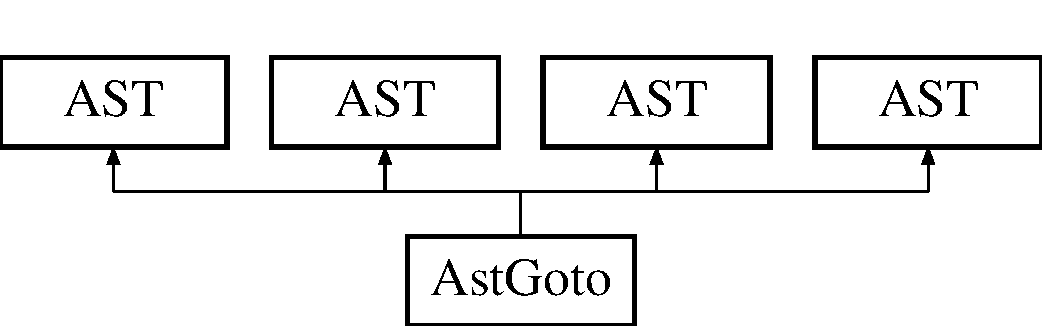
\includegraphics[height=2.000000cm]{classAstGoto}
\end{center}
\end{figure}
\subsection*{Public Member Functions}
\begin{DoxyCompactItemize}
\item 
void \hyperlink{classAstGoto_aa74c48ee01065e4cc79f686bdcfff22a}{Visit} ()
\begin{DoxyCompactList}\small\item\em This function is responsible for tree traversals. \end{DoxyCompactList}\item 
void \hyperlink{classAstGoto_aa74c48ee01065e4cc79f686bdcfff22a}{Visit} ()
\begin{DoxyCompactList}\small\item\em This function is responsible for tree traversals. \end{DoxyCompactList}\item 
void \hyperlink{classAstGoto_aa74c48ee01065e4cc79f686bdcfff22a}{Visit} ()
\begin{DoxyCompactList}\small\item\em This function is responsible for tree traversals. \end{DoxyCompactList}\item 
void \hyperlink{classAstGoto_aa74c48ee01065e4cc79f686bdcfff22a}{Visit} ()
\begin{DoxyCompactList}\small\item\em This function is responsible for tree traversals. \end{DoxyCompactList}\item 
void \hyperlink{classAST_a71d680856e95ff89f55d5311a552eba6}{set\-Label} (string l)
\begin{DoxyCompactList}\small\item\em Sets the label for the node. \end{DoxyCompactList}\item 
void \hyperlink{classAST_a71d680856e95ff89f55d5311a552eba6}{set\-Label} (string l)
\begin{DoxyCompactList}\small\item\em Sets the label for the node. \end{DoxyCompactList}\item 
void \hyperlink{classAST_a71d680856e95ff89f55d5311a552eba6}{set\-Label} (string l)
\begin{DoxyCompactList}\small\item\em Sets the label for the node. \end{DoxyCompactList}\item 
void \hyperlink{classAST_a71d680856e95ff89f55d5311a552eba6}{set\-Label} (string l)
\begin{DoxyCompactList}\small\item\em Sets the label for the node. \end{DoxyCompactList}\item 
int \hyperlink{classAST_ab7a5b1d9f1c2de0d98deb356f724a42c}{get\-U\-I\-D} ()
\begin{DoxyCompactList}\small\item\em Gets the node's unique I\-D. \end{DoxyCompactList}\item 
int \hyperlink{classAST_ab7a5b1d9f1c2de0d98deb356f724a42c}{get\-U\-I\-D} ()
\begin{DoxyCompactList}\small\item\em Gets the node's unique I\-D. \end{DoxyCompactList}\item 
int \hyperlink{classAST_ab7a5b1d9f1c2de0d98deb356f724a42c}{get\-U\-I\-D} ()
\begin{DoxyCompactList}\small\item\em Gets the node's unique I\-D. \end{DoxyCompactList}\item 
int \hyperlink{classAST_ab7a5b1d9f1c2de0d98deb356f724a42c}{get\-U\-I\-D} ()
\begin{DoxyCompactList}\small\item\em Gets the node's unique I\-D. \end{DoxyCompactList}\item 
string \hyperlink{classAST_aee029be902fffc927d16ccb03eb922ad}{get\-Label} ()
\begin{DoxyCompactList}\small\item\em Gets the node's label. \end{DoxyCompactList}\item 
string \hyperlink{classAST_aee029be902fffc927d16ccb03eb922ad}{get\-Label} ()
\begin{DoxyCompactList}\small\item\em Gets the node's label. \end{DoxyCompactList}\item 
string \hyperlink{classAST_aee029be902fffc927d16ccb03eb922ad}{get\-Label} ()
\begin{DoxyCompactList}\small\item\em Gets the node's label. \end{DoxyCompactList}\item 
string \hyperlink{classAST_aee029be902fffc927d16ccb03eb922ad}{get\-Label} ()
\begin{DoxyCompactList}\small\item\em Gets the node's label. \end{DoxyCompactList}\end{DoxyCompactItemize}
\subsection*{Public Attributes}
\begin{DoxyCompactItemize}
\item 
\hypertarget{classAST_aaf215802de409f8096c063d01ffa6783}{bool \hyperlink{classAST_aaf215802de409f8096c063d01ffa6783}{needs\-Cast}}\label{classAST_aaf215802de409f8096c063d01ffa6783}

\begin{DoxyCompactList}\small\item\em This indicates if cast 3\-A\-C needs to be output, and is only relevant for expressions. \end{DoxyCompactList}\item 
\hypertarget{classAST_afa9e77ef650ec6664458fa6cb55be985}{bool \hyperlink{classAST_afa9e77ef650ec6664458fa6cb55be985}{is\-Conv}}\label{classAST_afa9e77ef650ec6664458fa6cb55be985}

\begin{DoxyCompactList}\small\item\em Indicates is a conversion is possible. \end{DoxyCompactList}\item 
\hypertarget{classAST_a61ef3317e023d45237e06615b387cd6b}{C\-O\-N\-V\-E\-R\-S\-I\-O\-N\-T\-Y\-P\-E \hyperlink{classAST_a61ef3317e023d45237e06615b387cd6b}{conv\-Type}}\label{classAST_a61ef3317e023d45237e06615b387cd6b}

\begin{DoxyCompactList}\small\item\em If needs\-Cast is true, then this indicates what the cast should be. \end{DoxyCompactList}\item 
\hypertarget{classAST_aea9b07b39d24183f38c0029cec0a878e}{int \hyperlink{classAST_aea9b07b39d24183f38c0029cec0a878e}{operand\-To\-Cast}}\label{classAST_aea9b07b39d24183f38c0029cec0a878e}

\begin{DoxyCompactList}\small\item\em This indicates if the first or second operand should be the one that is cast. \end{DoxyCompactList}\end{DoxyCompactItemize}
\subsection*{Static Public Attributes}
\begin{DoxyCompactItemize}
\item 
\hypertarget{classAST_a5fdfd5f7b104dd92889163bdadbc68d6}{static \hyperlink{classVisualizer}{Visualizer} \hyperlink{classAST_a5fdfd5f7b104dd92889163bdadbc68d6}{vis}}\label{classAST_a5fdfd5f7b104dd92889163bdadbc68d6}

\begin{DoxyCompactList}\small\item\em Static visualizer instance for generating the visualization of the \hyperlink{classAST}{A\-S\-T}. \end{DoxyCompactList}\item 
\hypertarget{classAST_a8a3ace322f50e030331065d644ee55ee}{static \hyperlink{classTAC__Generator}{T\-A\-C\-\_\-\-Generator} \hyperlink{classAST_a8a3ace322f50e030331065d644ee55ee}{tac\-Gen}}\label{classAST_a8a3ace322f50e030331065d644ee55ee}

\begin{DoxyCompactList}\small\item\em Three address code generator. \end{DoxyCompactList}\item 
\hypertarget{classAST_a1f69448c6dc368d005631a128460083d}{static string {\bfseries current\-Temp} =\char`\"{}\char`\"{}}\label{classAST_a1f69448c6dc368d005631a128460083d}

\item 
\hypertarget{classAST_a551aec090c932ab69365238b40a8a4eb}{static string \hyperlink{classAST_a551aec090c932ab69365238b40a8a4eb}{return\-Label} =\char`\"{}\char`\"{}}\label{classAST_a551aec090c932ab69365238b40a8a4eb}

\begin{DoxyCompactList}\small\item\em This is for storing the string id of any temporary result register that may be created during 3\-A\-C generation. \end{DoxyCompactList}\item 
\hypertarget{classAST_a73c0a266df52be71e6b527b6aa635173}{static list$<$ string $>$ {\bfseries temp\-Stack}}\label{classAST_a73c0a266df52be71e6b527b6aa635173}

\item 
\hypertarget{classAST_abf9e84b541ff04b7bb64e6e4371512d4}{static string {\bfseries last\-I\-D} =\char`\"{}\char`\"{}}\label{classAST_abf9e84b541ff04b7bb64e6e4371512d4}

\item 
\hypertarget{classAST_a163003bfe9c30510ec8039870346049f}{static \hyperlink{classSymTab}{Sym\-Tab} $\ast$ {\bfseries symbol\-Table} =N\-U\-L\-L}\label{classAST_a163003bfe9c30510ec8039870346049f}

\item 
\hypertarget{classAST_a5c3cc894d9c0453523dec9ed76f18a04}{static string {\bfseries current\-Function} =\char`\"{}\char`\"{}}\label{classAST_a5c3cc894d9c0453523dec9ed76f18a04}

\item 
\hypertarget{classAST_a66155513b59ff1a04c8ece8b20ec31f5}{static int {\bfseries current\-Constant\-Value} =0}\label{classAST_a66155513b59ff1a04c8ece8b20ec31f5}

\item 
\hypertarget{classAST_a3d031d7bab635ba1f015aade5943f40c}{static string {\bfseries current\-Id\-Name} =\char`\"{}\char`\"{}}\label{classAST_a3d031d7bab635ba1f015aade5943f40c}

\item 
\hypertarget{classAST_a16c4b6e54febc1a26b31a64a46972ef0}{static int {\bfseries current\-Index\-Val} = 0}\label{classAST_a16c4b6e54febc1a26b31a64a46972ef0}

\end{DoxyCompactItemize}
\subsection*{Protected Attributes}
\begin{DoxyCompactItemize}
\item 
\hypertarget{classAST_a847b778f1c3dd5a19de32de432ee6e15}{int \hyperlink{classAST_a847b778f1c3dd5a19de32de432ee6e15}{uid}}\label{classAST_a847b778f1c3dd5a19de32de432ee6e15}

\begin{DoxyCompactList}\small\item\em The unique id. \end{DoxyCompactList}\item 
\hypertarget{classAST_ab2e239ccc0688d2341724432ff5a1a31}{string \hyperlink{classAST_ab2e239ccc0688d2341724432ff5a1a31}{label}}\label{classAST_ab2e239ccc0688d2341724432ff5a1a31}

\begin{DoxyCompactList}\small\item\em The label to be printed in the visualization. \end{DoxyCompactList}\end{DoxyCompactItemize}


\subsection{Detailed Description}


Definition at line 781 of file Ast.\-h.



\subsection{Member Function Documentation}
\hypertarget{classAST_aee029be902fffc927d16ccb03eb922ad}{\index{Ast\-Goto@{Ast\-Goto}!get\-Label@{get\-Label}}
\index{get\-Label@{get\-Label}!AstGoto@{Ast\-Goto}}
\subsubsection[{get\-Label}]{\setlength{\rightskip}{0pt plus 5cm}string A\-S\-T\-::get\-Label (
\begin{DoxyParamCaption}
{}
\end{DoxyParamCaption}
)\hspace{0.3cm}{\ttfamily [inline]}, {\ttfamily [inherited]}}}\label{classAST_aee029be902fffc927d16ccb03eb922ad}


Gets the node's label. 

\begin{DoxyReturn}{Returns}
The label 
\end{DoxyReturn}


Definition at line 60 of file Ast.\-h.

\hypertarget{classAST_aee029be902fffc927d16ccb03eb922ad}{\index{Ast\-Goto@{Ast\-Goto}!get\-Label@{get\-Label}}
\index{get\-Label@{get\-Label}!AstGoto@{Ast\-Goto}}
\subsubsection[{get\-Label}]{\setlength{\rightskip}{0pt plus 5cm}string A\-S\-T\-::get\-Label (
\begin{DoxyParamCaption}
{}
\end{DoxyParamCaption}
)\hspace{0.3cm}{\ttfamily [inline]}, {\ttfamily [inherited]}}}\label{classAST_aee029be902fffc927d16ccb03eb922ad}


Gets the node's label. 

\begin{DoxyReturn}{Returns}
The label 
\end{DoxyReturn}


Definition at line 60 of file C\-Scanner.\-ll.

\hypertarget{classAST_aee029be902fffc927d16ccb03eb922ad}{\index{Ast\-Goto@{Ast\-Goto}!get\-Label@{get\-Label}}
\index{get\-Label@{get\-Label}!AstGoto@{Ast\-Goto}}
\subsubsection[{get\-Label}]{\setlength{\rightskip}{0pt plus 5cm}string A\-S\-T\-::get\-Label (
\begin{DoxyParamCaption}
{}
\end{DoxyParamCaption}
)\hspace{0.3cm}{\ttfamily [inline]}, {\ttfamily [inherited]}}}\label{classAST_aee029be902fffc927d16ccb03eb922ad}


Gets the node's label. 

\begin{DoxyReturn}{Returns}
The label 
\end{DoxyReturn}


Definition at line 60 of file C\-Parser.\-yy.

\hypertarget{classAST_aee029be902fffc927d16ccb03eb922ad}{\index{Ast\-Goto@{Ast\-Goto}!get\-Label@{get\-Label}}
\index{get\-Label@{get\-Label}!AstGoto@{Ast\-Goto}}
\subsubsection[{get\-Label}]{\setlength{\rightskip}{0pt plus 5cm}string A\-S\-T\-::get\-Label (
\begin{DoxyParamCaption}
{}
\end{DoxyParamCaption}
)\hspace{0.3cm}{\ttfamily [inline]}, {\ttfamily [inherited]}}}\label{classAST_aee029be902fffc927d16ccb03eb922ad}


Gets the node's label. 

\begin{DoxyReturn}{Returns}
The label 
\end{DoxyReturn}


Definition at line 60 of file C\-Parser.\-yy.

\hypertarget{classAST_ab7a5b1d9f1c2de0d98deb356f724a42c}{\index{Ast\-Goto@{Ast\-Goto}!get\-U\-I\-D@{get\-U\-I\-D}}
\index{get\-U\-I\-D@{get\-U\-I\-D}!AstGoto@{Ast\-Goto}}
\subsubsection[{get\-U\-I\-D}]{\setlength{\rightskip}{0pt plus 5cm}int A\-S\-T\-::get\-U\-I\-D (
\begin{DoxyParamCaption}
{}
\end{DoxyParamCaption}
)\hspace{0.3cm}{\ttfamily [inline]}, {\ttfamily [inherited]}}}\label{classAST_ab7a5b1d9f1c2de0d98deb356f724a42c}


Gets the node's unique I\-D. 

\begin{DoxyReturn}{Returns}
The unique id 
\end{DoxyReturn}


Definition at line 53 of file C\-Parser.\-yy.

\hypertarget{classAST_ab7a5b1d9f1c2de0d98deb356f724a42c}{\index{Ast\-Goto@{Ast\-Goto}!get\-U\-I\-D@{get\-U\-I\-D}}
\index{get\-U\-I\-D@{get\-U\-I\-D}!AstGoto@{Ast\-Goto}}
\subsubsection[{get\-U\-I\-D}]{\setlength{\rightskip}{0pt plus 5cm}int A\-S\-T\-::get\-U\-I\-D (
\begin{DoxyParamCaption}
{}
\end{DoxyParamCaption}
)\hspace{0.3cm}{\ttfamily [inline]}, {\ttfamily [inherited]}}}\label{classAST_ab7a5b1d9f1c2de0d98deb356f724a42c}


Gets the node's unique I\-D. 

\begin{DoxyReturn}{Returns}
The unique id 
\end{DoxyReturn}


Definition at line 53 of file C\-Parser.\-yy.

\hypertarget{classAST_ab7a5b1d9f1c2de0d98deb356f724a42c}{\index{Ast\-Goto@{Ast\-Goto}!get\-U\-I\-D@{get\-U\-I\-D}}
\index{get\-U\-I\-D@{get\-U\-I\-D}!AstGoto@{Ast\-Goto}}
\subsubsection[{get\-U\-I\-D}]{\setlength{\rightskip}{0pt plus 5cm}int A\-S\-T\-::get\-U\-I\-D (
\begin{DoxyParamCaption}
{}
\end{DoxyParamCaption}
)\hspace{0.3cm}{\ttfamily [inline]}, {\ttfamily [inherited]}}}\label{classAST_ab7a5b1d9f1c2de0d98deb356f724a42c}


Gets the node's unique I\-D. 

\begin{DoxyReturn}{Returns}
The unique id 
\end{DoxyReturn}


Definition at line 53 of file C\-Scanner.\-ll.

\hypertarget{classAST_ab7a5b1d9f1c2de0d98deb356f724a42c}{\index{Ast\-Goto@{Ast\-Goto}!get\-U\-I\-D@{get\-U\-I\-D}}
\index{get\-U\-I\-D@{get\-U\-I\-D}!AstGoto@{Ast\-Goto}}
\subsubsection[{get\-U\-I\-D}]{\setlength{\rightskip}{0pt plus 5cm}int A\-S\-T\-::get\-U\-I\-D (
\begin{DoxyParamCaption}
{}
\end{DoxyParamCaption}
)\hspace{0.3cm}{\ttfamily [inline]}, {\ttfamily [inherited]}}}\label{classAST_ab7a5b1d9f1c2de0d98deb356f724a42c}


Gets the node's unique I\-D. 

\begin{DoxyReturn}{Returns}
The unique id 
\end{DoxyReturn}


Definition at line 53 of file Ast.\-h.

\hypertarget{classAST_a71d680856e95ff89f55d5311a552eba6}{\index{Ast\-Goto@{Ast\-Goto}!set\-Label@{set\-Label}}
\index{set\-Label@{set\-Label}!AstGoto@{Ast\-Goto}}
\subsubsection[{set\-Label}]{\setlength{\rightskip}{0pt plus 5cm}void A\-S\-T\-::set\-Label (
\begin{DoxyParamCaption}
\item[{string}]{l}
\end{DoxyParamCaption}
)\hspace{0.3cm}{\ttfamily [inline]}, {\ttfamily [inherited]}}}\label{classAST_a71d680856e95ff89f55d5311a552eba6}


Sets the label for the node. 


\begin{DoxyParams}{Parameters}
{\em l} & The label string \\
\hline
\end{DoxyParams}


Definition at line 43 of file C\-Scanner.\-ll.

\hypertarget{classAST_a71d680856e95ff89f55d5311a552eba6}{\index{Ast\-Goto@{Ast\-Goto}!set\-Label@{set\-Label}}
\index{set\-Label@{set\-Label}!AstGoto@{Ast\-Goto}}
\subsubsection[{set\-Label}]{\setlength{\rightskip}{0pt plus 5cm}void A\-S\-T\-::set\-Label (
\begin{DoxyParamCaption}
\item[{string}]{l}
\end{DoxyParamCaption}
)\hspace{0.3cm}{\ttfamily [inline]}, {\ttfamily [inherited]}}}\label{classAST_a71d680856e95ff89f55d5311a552eba6}


Sets the label for the node. 


\begin{DoxyParams}{Parameters}
{\em l} & The label string \\
\hline
\end{DoxyParams}


Definition at line 43 of file C\-Parser.\-yy.

\hypertarget{classAST_a71d680856e95ff89f55d5311a552eba6}{\index{Ast\-Goto@{Ast\-Goto}!set\-Label@{set\-Label}}
\index{set\-Label@{set\-Label}!AstGoto@{Ast\-Goto}}
\subsubsection[{set\-Label}]{\setlength{\rightskip}{0pt plus 5cm}void A\-S\-T\-::set\-Label (
\begin{DoxyParamCaption}
\item[{string}]{l}
\end{DoxyParamCaption}
)\hspace{0.3cm}{\ttfamily [inline]}, {\ttfamily [inherited]}}}\label{classAST_a71d680856e95ff89f55d5311a552eba6}


Sets the label for the node. 


\begin{DoxyParams}{Parameters}
{\em l} & The label string \\
\hline
\end{DoxyParams}


Definition at line 43 of file Ast.\-h.

\hypertarget{classAST_a71d680856e95ff89f55d5311a552eba6}{\index{Ast\-Goto@{Ast\-Goto}!set\-Label@{set\-Label}}
\index{set\-Label@{set\-Label}!AstGoto@{Ast\-Goto}}
\subsubsection[{set\-Label}]{\setlength{\rightskip}{0pt plus 5cm}void A\-S\-T\-::set\-Label (
\begin{DoxyParamCaption}
\item[{string}]{l}
\end{DoxyParamCaption}
)\hspace{0.3cm}{\ttfamily [inline]}, {\ttfamily [inherited]}}}\label{classAST_a71d680856e95ff89f55d5311a552eba6}


Sets the label for the node. 


\begin{DoxyParams}{Parameters}
{\em l} & The label string \\
\hline
\end{DoxyParams}


Definition at line 43 of file C\-Parser.\-yy.

\hypertarget{classAstGoto_aa74c48ee01065e4cc79f686bdcfff22a}{\index{Ast\-Goto@{Ast\-Goto}!Visit@{Visit}}
\index{Visit@{Visit}!AstGoto@{Ast\-Goto}}
\subsubsection[{Visit}]{\setlength{\rightskip}{0pt plus 5cm}void Ast\-Goto\-::\-Visit (
\begin{DoxyParamCaption}
{}
\end{DoxyParamCaption}
)\hspace{0.3cm}{\ttfamily [virtual]}}}\label{classAstGoto_aa74c48ee01065e4cc79f686bdcfff22a}


This function is responsible for tree traversals. 

This function will call the Visit functions of each of it's children nodes, call the visualization code for itself, and output any 3\-A\-C that can be generated at the current node. 

Reimplemented from \hyperlink{classAST_a5828cc86f2c4f1a0aeab6d7069e8fd82}{A\-S\-T}.



Definition at line 2110 of file Ast.\-cpp.

\hypertarget{classAstGoto_aa74c48ee01065e4cc79f686bdcfff22a}{\index{Ast\-Goto@{Ast\-Goto}!Visit@{Visit}}
\index{Visit@{Visit}!AstGoto@{Ast\-Goto}}
\subsubsection[{Visit}]{\setlength{\rightskip}{0pt plus 5cm}void Ast\-Goto\-::\-Visit (
\begin{DoxyParamCaption}
{}
\end{DoxyParamCaption}
)\hspace{0.3cm}{\ttfamily [virtual]}}}\label{classAstGoto_aa74c48ee01065e4cc79f686bdcfff22a}


This function is responsible for tree traversals. 

This function will call the Visit functions of each of it's children nodes, call the visualization code for itself, and output any 3\-A\-C that can be generated at the current node. 

Reimplemented from \hyperlink{classAST_a5828cc86f2c4f1a0aeab6d7069e8fd82}{A\-S\-T}.

\hypertarget{classAstGoto_aa74c48ee01065e4cc79f686bdcfff22a}{\index{Ast\-Goto@{Ast\-Goto}!Visit@{Visit}}
\index{Visit@{Visit}!AstGoto@{Ast\-Goto}}
\subsubsection[{Visit}]{\setlength{\rightskip}{0pt plus 5cm}void Ast\-Goto\-::\-Visit (
\begin{DoxyParamCaption}
{}
\end{DoxyParamCaption}
)\hspace{0.3cm}{\ttfamily [virtual]}}}\label{classAstGoto_aa74c48ee01065e4cc79f686bdcfff22a}


This function is responsible for tree traversals. 

This function will call the Visit functions of each of it's children nodes, call the visualization code for itself, and output any 3\-A\-C that can be generated at the current node. 

Reimplemented from \hyperlink{classAST_a5828cc86f2c4f1a0aeab6d7069e8fd82}{A\-S\-T}.

\hypertarget{classAstGoto_aa74c48ee01065e4cc79f686bdcfff22a}{\index{Ast\-Goto@{Ast\-Goto}!Visit@{Visit}}
\index{Visit@{Visit}!AstGoto@{Ast\-Goto}}
\subsubsection[{Visit}]{\setlength{\rightskip}{0pt plus 5cm}void Ast\-Goto\-::\-Visit (
\begin{DoxyParamCaption}
{}
\end{DoxyParamCaption}
)\hspace{0.3cm}{\ttfamily [virtual]}}}\label{classAstGoto_aa74c48ee01065e4cc79f686bdcfff22a}


This function is responsible for tree traversals. 

This function will call the Visit functions of each of it's children nodes, call the visualization code for itself, and output any 3\-A\-C that can be generated at the current node. 

Reimplemented from \hyperlink{classAST_a5828cc86f2c4f1a0aeab6d7069e8fd82}{A\-S\-T}.



The documentation for this class was generated from the following files\-:\begin{DoxyCompactItemize}
\item 
Ast.\-h\item 
Ast.\-cpp\end{DoxyCompactItemize}

\hypertarget{classAstID}{\section{Ast\-I\-D Class Reference}
\label{classAstID}\index{Ast\-I\-D@{Ast\-I\-D}}
}
Inheritance diagram for Ast\-I\-D\-:\begin{figure}[H]
\begin{center}
\leavevmode
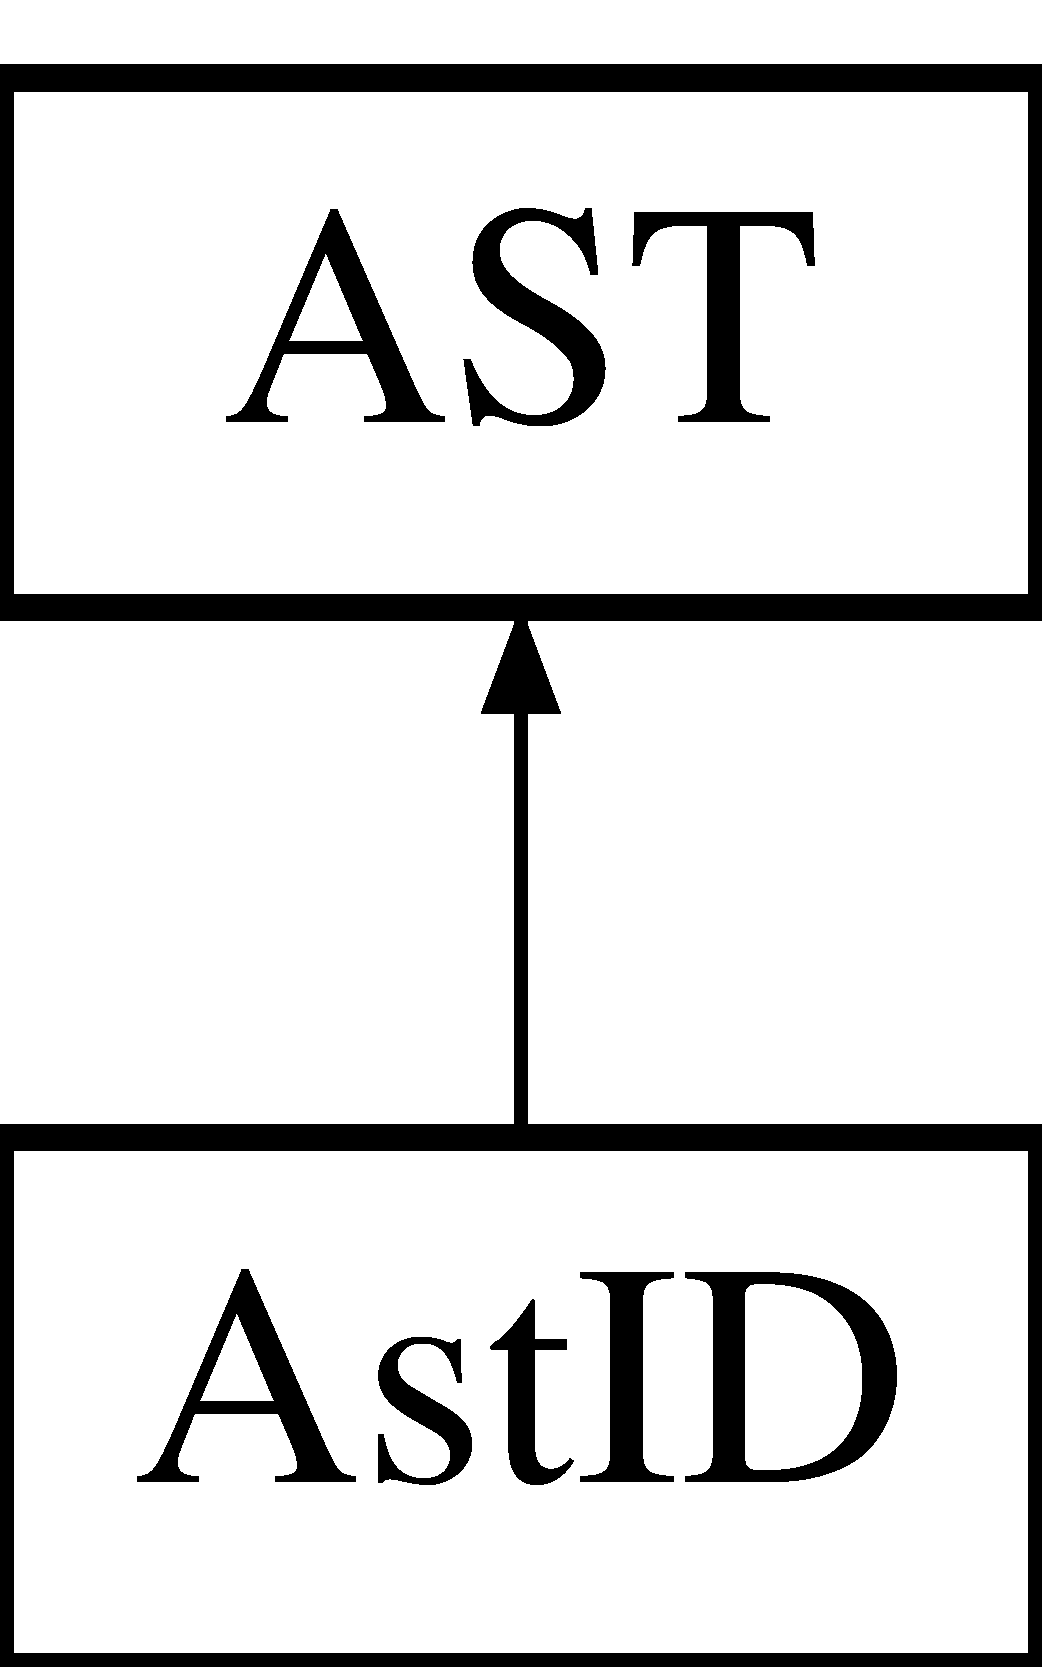
\includegraphics[height=2.000000cm]{classAstID}
\end{center}
\end{figure}
\subsection*{Public Member Functions}
\begin{DoxyCompactItemize}
\item 
\hypertarget{classAstID_a27fa9f77d0417f0368dd8433f742c18e}{{\bfseries Ast\-I\-D} (string s, \hyperlink{classType}{Type} $\ast$t)}\label{classAstID_a27fa9f77d0417f0368dd8433f742c18e}

\item 
\hypertarget{classAstID_a2ff55dfac7babf1a4649ab10f3a02f3d}{string {\bfseries Get\-Name} ()}\label{classAstID_a2ff55dfac7babf1a4649ab10f3a02f3d}

\item 
void \hyperlink{classAstID_af84d100fc8e77d534362310f36855ad0}{Visit} ()
\begin{DoxyCompactList}\small\item\em This function is responsible for tree traversals. \end{DoxyCompactList}\item 
\hypertarget{classAstID_a27fa9f77d0417f0368dd8433f742c18e}{{\bfseries Ast\-I\-D} (string s, \hyperlink{classType}{Type} $\ast$t)}\label{classAstID_a27fa9f77d0417f0368dd8433f742c18e}

\item 
\hypertarget{classAstID_a2ff55dfac7babf1a4649ab10f3a02f3d}{string {\bfseries Get\-Name} ()}\label{classAstID_a2ff55dfac7babf1a4649ab10f3a02f3d}

\item 
void \hyperlink{classAstID_af84d100fc8e77d534362310f36855ad0}{Visit} ()
\begin{DoxyCompactList}\small\item\em This function is responsible for tree traversals. \end{DoxyCompactList}\item 
\hypertarget{classAstID_a27fa9f77d0417f0368dd8433f742c18e}{{\bfseries Ast\-I\-D} (string s, \hyperlink{classType}{Type} $\ast$t)}\label{classAstID_a27fa9f77d0417f0368dd8433f742c18e}

\item 
\hypertarget{classAstID_a2ff55dfac7babf1a4649ab10f3a02f3d}{string {\bfseries Get\-Name} ()}\label{classAstID_a2ff55dfac7babf1a4649ab10f3a02f3d}

\item 
void \hyperlink{classAstID_af84d100fc8e77d534362310f36855ad0}{Visit} ()
\begin{DoxyCompactList}\small\item\em This function is responsible for tree traversals. \end{DoxyCompactList}\item 
\hypertarget{classAstID_a27fa9f77d0417f0368dd8433f742c18e}{{\bfseries Ast\-I\-D} (string s, \hyperlink{classType}{Type} $\ast$t)}\label{classAstID_a27fa9f77d0417f0368dd8433f742c18e}

\item 
\hypertarget{classAstID_a2ff55dfac7babf1a4649ab10f3a02f3d}{string {\bfseries Get\-Name} ()}\label{classAstID_a2ff55dfac7babf1a4649ab10f3a02f3d}

\item 
void \hyperlink{classAstID_af84d100fc8e77d534362310f36855ad0}{Visit} ()
\begin{DoxyCompactList}\small\item\em This function is responsible for tree traversals. \end{DoxyCompactList}\item 
void \hyperlink{classAST_a71d680856e95ff89f55d5311a552eba6}{set\-Label} (string l)
\begin{DoxyCompactList}\small\item\em Sets the label for the node. \end{DoxyCompactList}\item 
void \hyperlink{classAST_a71d680856e95ff89f55d5311a552eba6}{set\-Label} (string l)
\begin{DoxyCompactList}\small\item\em Sets the label for the node. \end{DoxyCompactList}\item 
void \hyperlink{classAST_a71d680856e95ff89f55d5311a552eba6}{set\-Label} (string l)
\begin{DoxyCompactList}\small\item\em Sets the label for the node. \end{DoxyCompactList}\item 
void \hyperlink{classAST_a71d680856e95ff89f55d5311a552eba6}{set\-Label} (string l)
\begin{DoxyCompactList}\small\item\em Sets the label for the node. \end{DoxyCompactList}\item 
int \hyperlink{classAST_ab7a5b1d9f1c2de0d98deb356f724a42c}{get\-U\-I\-D} ()
\begin{DoxyCompactList}\small\item\em Gets the node's unique I\-D. \end{DoxyCompactList}\item 
int \hyperlink{classAST_ab7a5b1d9f1c2de0d98deb356f724a42c}{get\-U\-I\-D} ()
\begin{DoxyCompactList}\small\item\em Gets the node's unique I\-D. \end{DoxyCompactList}\item 
int \hyperlink{classAST_ab7a5b1d9f1c2de0d98deb356f724a42c}{get\-U\-I\-D} ()
\begin{DoxyCompactList}\small\item\em Gets the node's unique I\-D. \end{DoxyCompactList}\item 
int \hyperlink{classAST_ab7a5b1d9f1c2de0d98deb356f724a42c}{get\-U\-I\-D} ()
\begin{DoxyCompactList}\small\item\em Gets the node's unique I\-D. \end{DoxyCompactList}\item 
string \hyperlink{classAST_aee029be902fffc927d16ccb03eb922ad}{get\-Label} ()
\begin{DoxyCompactList}\small\item\em Gets the node's label. \end{DoxyCompactList}\item 
string \hyperlink{classAST_aee029be902fffc927d16ccb03eb922ad}{get\-Label} ()
\begin{DoxyCompactList}\small\item\em Gets the node's label. \end{DoxyCompactList}\item 
string \hyperlink{classAST_aee029be902fffc927d16ccb03eb922ad}{get\-Label} ()
\begin{DoxyCompactList}\small\item\em Gets the node's label. \end{DoxyCompactList}\item 
string \hyperlink{classAST_aee029be902fffc927d16ccb03eb922ad}{get\-Label} ()
\begin{DoxyCompactList}\small\item\em Gets the node's label. \end{DoxyCompactList}\end{DoxyCompactItemize}
\subsection*{Public Attributes}
\begin{DoxyCompactItemize}
\item 
\hypertarget{classAstID_ab7c45d962591b1ea1785d2595f1b6497}{string {\bfseries str}}\label{classAstID_ab7c45d962591b1ea1785d2595f1b6497}

\item 
\hypertarget{classAstID_a963e4044d140b100ef56bc49b7f97481}{\hyperlink{classType}{Type} $\ast$ {\bfseries type}}\label{classAstID_a963e4044d140b100ef56bc49b7f97481}

\item 
\hypertarget{classAST_aaf215802de409f8096c063d01ffa6783}{bool \hyperlink{classAST_aaf215802de409f8096c063d01ffa6783}{needs\-Cast}}\label{classAST_aaf215802de409f8096c063d01ffa6783}

\begin{DoxyCompactList}\small\item\em This indicates if cast 3\-A\-C needs to be output, and is only relevant for expressions. \end{DoxyCompactList}\item 
\hypertarget{classAST_afa9e77ef650ec6664458fa6cb55be985}{bool \hyperlink{classAST_afa9e77ef650ec6664458fa6cb55be985}{is\-Conv}}\label{classAST_afa9e77ef650ec6664458fa6cb55be985}

\begin{DoxyCompactList}\small\item\em Indicates is a conversion is possible. \end{DoxyCompactList}\item 
\hypertarget{classAST_a61ef3317e023d45237e06615b387cd6b}{C\-O\-N\-V\-E\-R\-S\-I\-O\-N\-T\-Y\-P\-E \hyperlink{classAST_a61ef3317e023d45237e06615b387cd6b}{conv\-Type}}\label{classAST_a61ef3317e023d45237e06615b387cd6b}

\begin{DoxyCompactList}\small\item\em If needs\-Cast is true, then this indicates what the cast should be. \end{DoxyCompactList}\item 
\hypertarget{classAST_aea9b07b39d24183f38c0029cec0a878e}{int \hyperlink{classAST_aea9b07b39d24183f38c0029cec0a878e}{operand\-To\-Cast}}\label{classAST_aea9b07b39d24183f38c0029cec0a878e}

\begin{DoxyCompactList}\small\item\em This indicates if the first or second operand should be the one that is cast. \end{DoxyCompactList}\end{DoxyCompactItemize}
\subsection*{Static Public Attributes}
\begin{DoxyCompactItemize}
\item 
\hypertarget{classAST_a5fdfd5f7b104dd92889163bdadbc68d6}{static \hyperlink{classVisualizer}{Visualizer} \hyperlink{classAST_a5fdfd5f7b104dd92889163bdadbc68d6}{vis}}\label{classAST_a5fdfd5f7b104dd92889163bdadbc68d6}

\begin{DoxyCompactList}\small\item\em Static visualizer instance for generating the visualization of the \hyperlink{classAST}{A\-S\-T}. \end{DoxyCompactList}\item 
\hypertarget{classAST_a8a3ace322f50e030331065d644ee55ee}{static \hyperlink{classTAC__Generator}{T\-A\-C\-\_\-\-Generator} \hyperlink{classAST_a8a3ace322f50e030331065d644ee55ee}{tac\-Gen}}\label{classAST_a8a3ace322f50e030331065d644ee55ee}

\begin{DoxyCompactList}\small\item\em Three address code generator. \end{DoxyCompactList}\item 
\hypertarget{classAST_a1f69448c6dc368d005631a128460083d}{static string {\bfseries current\-Temp} =\char`\"{}\char`\"{}}\label{classAST_a1f69448c6dc368d005631a128460083d}

\item 
\hypertarget{classAST_a551aec090c932ab69365238b40a8a4eb}{static string \hyperlink{classAST_a551aec090c932ab69365238b40a8a4eb}{return\-Label} =\char`\"{}\char`\"{}}\label{classAST_a551aec090c932ab69365238b40a8a4eb}

\begin{DoxyCompactList}\small\item\em This is for storing the string id of any temporary result register that may be created during 3\-A\-C generation. \end{DoxyCompactList}\item 
\hypertarget{classAST_a73c0a266df52be71e6b527b6aa635173}{static list$<$ string $>$ {\bfseries temp\-Stack}}\label{classAST_a73c0a266df52be71e6b527b6aa635173}

\item 
\hypertarget{classAST_abf9e84b541ff04b7bb64e6e4371512d4}{static string {\bfseries last\-I\-D} =\char`\"{}\char`\"{}}\label{classAST_abf9e84b541ff04b7bb64e6e4371512d4}

\item 
\hypertarget{classAST_a163003bfe9c30510ec8039870346049f}{static \hyperlink{classSymTab}{Sym\-Tab} $\ast$ {\bfseries symbol\-Table} =N\-U\-L\-L}\label{classAST_a163003bfe9c30510ec8039870346049f}

\item 
\hypertarget{classAST_a5c3cc894d9c0453523dec9ed76f18a04}{static string {\bfseries current\-Function} =\char`\"{}\char`\"{}}\label{classAST_a5c3cc894d9c0453523dec9ed76f18a04}

\item 
\hypertarget{classAST_a66155513b59ff1a04c8ece8b20ec31f5}{static int {\bfseries current\-Constant\-Value} =0}\label{classAST_a66155513b59ff1a04c8ece8b20ec31f5}

\item 
\hypertarget{classAST_a3d031d7bab635ba1f015aade5943f40c}{static string {\bfseries current\-Id\-Name} =\char`\"{}\char`\"{}}\label{classAST_a3d031d7bab635ba1f015aade5943f40c}

\item 
\hypertarget{classAST_a16c4b6e54febc1a26b31a64a46972ef0}{static int {\bfseries current\-Index\-Val} = 0}\label{classAST_a16c4b6e54febc1a26b31a64a46972ef0}

\item 
\hypertarget{classAST_a6fc65ae9dd064a88941d4b88669b19db}{static string {\bfseries current\-I\-D} = \char`\"{}\char`\"{}}\label{classAST_a6fc65ae9dd064a88941d4b88669b19db}

\end{DoxyCompactItemize}
\subsection*{Protected Attributes}
\begin{DoxyCompactItemize}
\item 
\hypertarget{classAST_a847b778f1c3dd5a19de32de432ee6e15}{int \hyperlink{classAST_a847b778f1c3dd5a19de32de432ee6e15}{uid}}\label{classAST_a847b778f1c3dd5a19de32de432ee6e15}

\begin{DoxyCompactList}\small\item\em The unique id. \end{DoxyCompactList}\item 
\hypertarget{classAST_ab2e239ccc0688d2341724432ff5a1a31}{string \hyperlink{classAST_ab2e239ccc0688d2341724432ff5a1a31}{label}}\label{classAST_ab2e239ccc0688d2341724432ff5a1a31}

\begin{DoxyCompactList}\small\item\em The label to be printed in the visualization. \end{DoxyCompactList}\end{DoxyCompactItemize}


\subsection{Detailed Description}


Definition at line 228 of file Ast.\-h.



\subsection{Member Function Documentation}
\hypertarget{classAST_aee029be902fffc927d16ccb03eb922ad}{\index{Ast\-I\-D@{Ast\-I\-D}!get\-Label@{get\-Label}}
\index{get\-Label@{get\-Label}!AstID@{Ast\-I\-D}}
\subsubsection[{get\-Label}]{\setlength{\rightskip}{0pt plus 5cm}string A\-S\-T\-::get\-Label (
\begin{DoxyParamCaption}
{}
\end{DoxyParamCaption}
)\hspace{0.3cm}{\ttfamily [inline]}, {\ttfamily [inherited]}}}\label{classAST_aee029be902fffc927d16ccb03eb922ad}


Gets the node's label. 

\begin{DoxyReturn}{Returns}
The label 
\end{DoxyReturn}


Definition at line 60 of file Ast.\-h.

\hypertarget{classAST_aee029be902fffc927d16ccb03eb922ad}{\index{Ast\-I\-D@{Ast\-I\-D}!get\-Label@{get\-Label}}
\index{get\-Label@{get\-Label}!AstID@{Ast\-I\-D}}
\subsubsection[{get\-Label}]{\setlength{\rightskip}{0pt plus 5cm}string A\-S\-T\-::get\-Label (
\begin{DoxyParamCaption}
{}
\end{DoxyParamCaption}
)\hspace{0.3cm}{\ttfamily [inline]}, {\ttfamily [inherited]}}}\label{classAST_aee029be902fffc927d16ccb03eb922ad}


Gets the node's label. 

\begin{DoxyReturn}{Returns}
The label 
\end{DoxyReturn}


Definition at line 60 of file C\-Parser.\-yy.

\hypertarget{classAST_aee029be902fffc927d16ccb03eb922ad}{\index{Ast\-I\-D@{Ast\-I\-D}!get\-Label@{get\-Label}}
\index{get\-Label@{get\-Label}!AstID@{Ast\-I\-D}}
\subsubsection[{get\-Label}]{\setlength{\rightskip}{0pt plus 5cm}string A\-S\-T\-::get\-Label (
\begin{DoxyParamCaption}
{}
\end{DoxyParamCaption}
)\hspace{0.3cm}{\ttfamily [inline]}, {\ttfamily [inherited]}}}\label{classAST_aee029be902fffc927d16ccb03eb922ad}


Gets the node's label. 

\begin{DoxyReturn}{Returns}
The label 
\end{DoxyReturn}


Definition at line 60 of file C\-Parser.\-yy.

\hypertarget{classAST_aee029be902fffc927d16ccb03eb922ad}{\index{Ast\-I\-D@{Ast\-I\-D}!get\-Label@{get\-Label}}
\index{get\-Label@{get\-Label}!AstID@{Ast\-I\-D}}
\subsubsection[{get\-Label}]{\setlength{\rightskip}{0pt plus 5cm}string A\-S\-T\-::get\-Label (
\begin{DoxyParamCaption}
{}
\end{DoxyParamCaption}
)\hspace{0.3cm}{\ttfamily [inline]}, {\ttfamily [inherited]}}}\label{classAST_aee029be902fffc927d16ccb03eb922ad}


Gets the node's label. 

\begin{DoxyReturn}{Returns}
The label 
\end{DoxyReturn}


Definition at line 60 of file C\-Scanner.\-ll.

\hypertarget{classAST_ab7a5b1d9f1c2de0d98deb356f724a42c}{\index{Ast\-I\-D@{Ast\-I\-D}!get\-U\-I\-D@{get\-U\-I\-D}}
\index{get\-U\-I\-D@{get\-U\-I\-D}!AstID@{Ast\-I\-D}}
\subsubsection[{get\-U\-I\-D}]{\setlength{\rightskip}{0pt plus 5cm}int A\-S\-T\-::get\-U\-I\-D (
\begin{DoxyParamCaption}
{}
\end{DoxyParamCaption}
)\hspace{0.3cm}{\ttfamily [inline]}, {\ttfamily [inherited]}}}\label{classAST_ab7a5b1d9f1c2de0d98deb356f724a42c}


Gets the node's unique I\-D. 

\begin{DoxyReturn}{Returns}
The unique id 
\end{DoxyReturn}


Definition at line 53 of file C\-Scanner.\-ll.

\hypertarget{classAST_ab7a5b1d9f1c2de0d98deb356f724a42c}{\index{Ast\-I\-D@{Ast\-I\-D}!get\-U\-I\-D@{get\-U\-I\-D}}
\index{get\-U\-I\-D@{get\-U\-I\-D}!AstID@{Ast\-I\-D}}
\subsubsection[{get\-U\-I\-D}]{\setlength{\rightskip}{0pt plus 5cm}int A\-S\-T\-::get\-U\-I\-D (
\begin{DoxyParamCaption}
{}
\end{DoxyParamCaption}
)\hspace{0.3cm}{\ttfamily [inline]}, {\ttfamily [inherited]}}}\label{classAST_ab7a5b1d9f1c2de0d98deb356f724a42c}


Gets the node's unique I\-D. 

\begin{DoxyReturn}{Returns}
The unique id 
\end{DoxyReturn}


Definition at line 53 of file C\-Parser.\-yy.

\hypertarget{classAST_ab7a5b1d9f1c2de0d98deb356f724a42c}{\index{Ast\-I\-D@{Ast\-I\-D}!get\-U\-I\-D@{get\-U\-I\-D}}
\index{get\-U\-I\-D@{get\-U\-I\-D}!AstID@{Ast\-I\-D}}
\subsubsection[{get\-U\-I\-D}]{\setlength{\rightskip}{0pt plus 5cm}int A\-S\-T\-::get\-U\-I\-D (
\begin{DoxyParamCaption}
{}
\end{DoxyParamCaption}
)\hspace{0.3cm}{\ttfamily [inline]}, {\ttfamily [inherited]}}}\label{classAST_ab7a5b1d9f1c2de0d98deb356f724a42c}


Gets the node's unique I\-D. 

\begin{DoxyReturn}{Returns}
The unique id 
\end{DoxyReturn}


Definition at line 53 of file Ast.\-h.

\hypertarget{classAST_ab7a5b1d9f1c2de0d98deb356f724a42c}{\index{Ast\-I\-D@{Ast\-I\-D}!get\-U\-I\-D@{get\-U\-I\-D}}
\index{get\-U\-I\-D@{get\-U\-I\-D}!AstID@{Ast\-I\-D}}
\subsubsection[{get\-U\-I\-D}]{\setlength{\rightskip}{0pt plus 5cm}int A\-S\-T\-::get\-U\-I\-D (
\begin{DoxyParamCaption}
{}
\end{DoxyParamCaption}
)\hspace{0.3cm}{\ttfamily [inline]}, {\ttfamily [inherited]}}}\label{classAST_ab7a5b1d9f1c2de0d98deb356f724a42c}


Gets the node's unique I\-D. 

\begin{DoxyReturn}{Returns}
The unique id 
\end{DoxyReturn}


Definition at line 53 of file C\-Parser.\-yy.

\hypertarget{classAST_a71d680856e95ff89f55d5311a552eba6}{\index{Ast\-I\-D@{Ast\-I\-D}!set\-Label@{set\-Label}}
\index{set\-Label@{set\-Label}!AstID@{Ast\-I\-D}}
\subsubsection[{set\-Label}]{\setlength{\rightskip}{0pt plus 5cm}void A\-S\-T\-::set\-Label (
\begin{DoxyParamCaption}
\item[{string}]{l}
\end{DoxyParamCaption}
)\hspace{0.3cm}{\ttfamily [inline]}, {\ttfamily [inherited]}}}\label{classAST_a71d680856e95ff89f55d5311a552eba6}


Sets the label for the node. 


\begin{DoxyParams}{Parameters}
{\em l} & The label string \\
\hline
\end{DoxyParams}


Definition at line 43 of file C\-Scanner.\-ll.

\hypertarget{classAST_a71d680856e95ff89f55d5311a552eba6}{\index{Ast\-I\-D@{Ast\-I\-D}!set\-Label@{set\-Label}}
\index{set\-Label@{set\-Label}!AstID@{Ast\-I\-D}}
\subsubsection[{set\-Label}]{\setlength{\rightskip}{0pt plus 5cm}void A\-S\-T\-::set\-Label (
\begin{DoxyParamCaption}
\item[{string}]{l}
\end{DoxyParamCaption}
)\hspace{0.3cm}{\ttfamily [inline]}, {\ttfamily [inherited]}}}\label{classAST_a71d680856e95ff89f55d5311a552eba6}


Sets the label for the node. 


\begin{DoxyParams}{Parameters}
{\em l} & The label string \\
\hline
\end{DoxyParams}


Definition at line 43 of file Ast.\-h.

\hypertarget{classAST_a71d680856e95ff89f55d5311a552eba6}{\index{Ast\-I\-D@{Ast\-I\-D}!set\-Label@{set\-Label}}
\index{set\-Label@{set\-Label}!AstID@{Ast\-I\-D}}
\subsubsection[{set\-Label}]{\setlength{\rightskip}{0pt plus 5cm}void A\-S\-T\-::set\-Label (
\begin{DoxyParamCaption}
\item[{string}]{l}
\end{DoxyParamCaption}
)\hspace{0.3cm}{\ttfamily [inline]}, {\ttfamily [inherited]}}}\label{classAST_a71d680856e95ff89f55d5311a552eba6}


Sets the label for the node. 


\begin{DoxyParams}{Parameters}
{\em l} & The label string \\
\hline
\end{DoxyParams}


Definition at line 43 of file C\-Parser.\-yy.

\hypertarget{classAST_a71d680856e95ff89f55d5311a552eba6}{\index{Ast\-I\-D@{Ast\-I\-D}!set\-Label@{set\-Label}}
\index{set\-Label@{set\-Label}!AstID@{Ast\-I\-D}}
\subsubsection[{set\-Label}]{\setlength{\rightskip}{0pt plus 5cm}void A\-S\-T\-::set\-Label (
\begin{DoxyParamCaption}
\item[{string}]{l}
\end{DoxyParamCaption}
)\hspace{0.3cm}{\ttfamily [inline]}, {\ttfamily [inherited]}}}\label{classAST_a71d680856e95ff89f55d5311a552eba6}


Sets the label for the node. 


\begin{DoxyParams}{Parameters}
{\em l} & The label string \\
\hline
\end{DoxyParams}


Definition at line 43 of file C\-Parser.\-yy.

\hypertarget{classAstID_af84d100fc8e77d534362310f36855ad0}{\index{Ast\-I\-D@{Ast\-I\-D}!Visit@{Visit}}
\index{Visit@{Visit}!AstID@{Ast\-I\-D}}
\subsubsection[{Visit}]{\setlength{\rightskip}{0pt plus 5cm}void Ast\-I\-D\-::\-Visit (
\begin{DoxyParamCaption}
{}
\end{DoxyParamCaption}
)\hspace{0.3cm}{\ttfamily [virtual]}}}\label{classAstID_af84d100fc8e77d534362310f36855ad0}


This function is responsible for tree traversals. 

This function will call the Visit functions of each of it's children nodes, call the visualization code for itself, and output any 3\-A\-C that can be generated at the current node. 

Reimplemented from \hyperlink{classAST_a5828cc86f2c4f1a0aeab6d7069e8fd82}{A\-S\-T}.

\hypertarget{classAstID_af84d100fc8e77d534362310f36855ad0}{\index{Ast\-I\-D@{Ast\-I\-D}!Visit@{Visit}}
\index{Visit@{Visit}!AstID@{Ast\-I\-D}}
\subsubsection[{Visit}]{\setlength{\rightskip}{0pt plus 5cm}void Ast\-I\-D\-::\-Visit (
\begin{DoxyParamCaption}
{}
\end{DoxyParamCaption}
)\hspace{0.3cm}{\ttfamily [virtual]}}}\label{classAstID_af84d100fc8e77d534362310f36855ad0}


This function is responsible for tree traversals. 

This function will call the Visit functions of each of it's children nodes, call the visualization code for itself, and output any 3\-A\-C that can be generated at the current node. 

Reimplemented from \hyperlink{classAST_a5828cc86f2c4f1a0aeab6d7069e8fd82}{A\-S\-T}.

\hypertarget{classAstID_af84d100fc8e77d534362310f36855ad0}{\index{Ast\-I\-D@{Ast\-I\-D}!Visit@{Visit}}
\index{Visit@{Visit}!AstID@{Ast\-I\-D}}
\subsubsection[{Visit}]{\setlength{\rightskip}{0pt plus 5cm}void Ast\-I\-D\-::\-Visit (
\begin{DoxyParamCaption}
{}
\end{DoxyParamCaption}
)\hspace{0.3cm}{\ttfamily [virtual]}}}\label{classAstID_af84d100fc8e77d534362310f36855ad0}


This function is responsible for tree traversals. 

This function will call the Visit functions of each of it's children nodes, call the visualization code for itself, and output any 3\-A\-C that can be generated at the current node. 

Reimplemented from \hyperlink{classAST_a5828cc86f2c4f1a0aeab6d7069e8fd82}{A\-S\-T}.

\hypertarget{classAstID_af84d100fc8e77d534362310f36855ad0}{\index{Ast\-I\-D@{Ast\-I\-D}!Visit@{Visit}}
\index{Visit@{Visit}!AstID@{Ast\-I\-D}}
\subsubsection[{Visit}]{\setlength{\rightskip}{0pt plus 5cm}void Ast\-I\-D\-::\-Visit (
\begin{DoxyParamCaption}
{}
\end{DoxyParamCaption}
)\hspace{0.3cm}{\ttfamily [virtual]}}}\label{classAstID_af84d100fc8e77d534362310f36855ad0}


This function is responsible for tree traversals. 

This function will call the Visit functions of each of it's children nodes, call the visualization code for itself, and output any 3\-A\-C that can be generated at the current node. 

Reimplemented from \hyperlink{classAST_a5828cc86f2c4f1a0aeab6d7069e8fd82}{A\-S\-T}.



Definition at line 1004 of file Ast.\-cpp.



The documentation for this class was generated from the following files\-:\begin{DoxyCompactItemize}
\item 
Ast.\-h\item 
Ast.\-cpp\end{DoxyCompactItemize}

\input{classAstIDList}
\hypertarget{classAstIfElse}{\section{Ast\-If\-Else Class Reference}
\label{classAstIfElse}\index{Ast\-If\-Else@{Ast\-If\-Else}}
}
Inheritance diagram for Ast\-If\-Else\-:\begin{figure}[H]
\begin{center}
\leavevmode
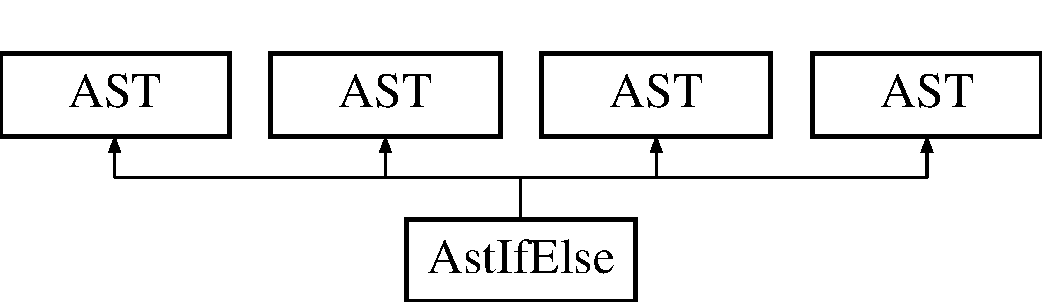
\includegraphics[height=2.000000cm]{classAstIfElse}
\end{center}
\end{figure}
\subsection*{Public Member Functions}
\begin{DoxyCompactItemize}
\item 
\hypertarget{classAstIfElse_aac4a0ab9c36999fdd491ef5fe6c1e68c}{{\bfseries Ast\-If\-Else} (\hyperlink{classAstExpression}{Ast\-Expression} $\ast$test, \hyperlink{classAstStatement}{Ast\-Statement} $\ast$statement, \hyperlink{classAstStatement}{Ast\-Statement} $\ast$else\-Statement)}\label{classAstIfElse_aac4a0ab9c36999fdd491ef5fe6c1e68c}

\item 
void \hyperlink{classAstIfElse_a4c038fd5b0cb99ea75f9847d96f65c32}{Visit} ()
\begin{DoxyCompactList}\small\item\em This function is responsible for tree traversals. \end{DoxyCompactList}\item 
\hypertarget{classAstIfElse_aac4a0ab9c36999fdd491ef5fe6c1e68c}{{\bfseries Ast\-If\-Else} (\hyperlink{classAstExpression}{Ast\-Expression} $\ast$test, \hyperlink{classAstStatement}{Ast\-Statement} $\ast$statement, \hyperlink{classAstStatement}{Ast\-Statement} $\ast$else\-Statement)}\label{classAstIfElse_aac4a0ab9c36999fdd491ef5fe6c1e68c}

\item 
void \hyperlink{classAstIfElse_a4c038fd5b0cb99ea75f9847d96f65c32}{Visit} ()
\begin{DoxyCompactList}\small\item\em This function is responsible for tree traversals. \end{DoxyCompactList}\item 
\hypertarget{classAstIfElse_aac4a0ab9c36999fdd491ef5fe6c1e68c}{{\bfseries Ast\-If\-Else} (\hyperlink{classAstExpression}{Ast\-Expression} $\ast$test, \hyperlink{classAstStatement}{Ast\-Statement} $\ast$statement, \hyperlink{classAstStatement}{Ast\-Statement} $\ast$else\-Statement)}\label{classAstIfElse_aac4a0ab9c36999fdd491ef5fe6c1e68c}

\item 
void \hyperlink{classAstIfElse_a4c038fd5b0cb99ea75f9847d96f65c32}{Visit} ()
\begin{DoxyCompactList}\small\item\em This function is responsible for tree traversals. \end{DoxyCompactList}\item 
\hypertarget{classAstIfElse_aac4a0ab9c36999fdd491ef5fe6c1e68c}{{\bfseries Ast\-If\-Else} (\hyperlink{classAstExpression}{Ast\-Expression} $\ast$test, \hyperlink{classAstStatement}{Ast\-Statement} $\ast$statement, \hyperlink{classAstStatement}{Ast\-Statement} $\ast$else\-Statement)}\label{classAstIfElse_aac4a0ab9c36999fdd491ef5fe6c1e68c}

\item 
void \hyperlink{classAstIfElse_a4c038fd5b0cb99ea75f9847d96f65c32}{Visit} ()
\begin{DoxyCompactList}\small\item\em This function is responsible for tree traversals. \end{DoxyCompactList}\item 
void \hyperlink{classAST_a71d680856e95ff89f55d5311a552eba6}{set\-Label} (string l)
\begin{DoxyCompactList}\small\item\em Sets the label for the node. \end{DoxyCompactList}\item 
void \hyperlink{classAST_a71d680856e95ff89f55d5311a552eba6}{set\-Label} (string l)
\begin{DoxyCompactList}\small\item\em Sets the label for the node. \end{DoxyCompactList}\item 
void \hyperlink{classAST_a71d680856e95ff89f55d5311a552eba6}{set\-Label} (string l)
\begin{DoxyCompactList}\small\item\em Sets the label for the node. \end{DoxyCompactList}\item 
void \hyperlink{classAST_a71d680856e95ff89f55d5311a552eba6}{set\-Label} (string l)
\begin{DoxyCompactList}\small\item\em Sets the label for the node. \end{DoxyCompactList}\item 
int \hyperlink{classAST_ab7a5b1d9f1c2de0d98deb356f724a42c}{get\-U\-I\-D} ()
\begin{DoxyCompactList}\small\item\em Gets the node's unique I\-D. \end{DoxyCompactList}\item 
int \hyperlink{classAST_ab7a5b1d9f1c2de0d98deb356f724a42c}{get\-U\-I\-D} ()
\begin{DoxyCompactList}\small\item\em Gets the node's unique I\-D. \end{DoxyCompactList}\item 
int \hyperlink{classAST_ab7a5b1d9f1c2de0d98deb356f724a42c}{get\-U\-I\-D} ()
\begin{DoxyCompactList}\small\item\em Gets the node's unique I\-D. \end{DoxyCompactList}\item 
int \hyperlink{classAST_ab7a5b1d9f1c2de0d98deb356f724a42c}{get\-U\-I\-D} ()
\begin{DoxyCompactList}\small\item\em Gets the node's unique I\-D. \end{DoxyCompactList}\item 
string \hyperlink{classAST_aee029be902fffc927d16ccb03eb922ad}{get\-Label} ()
\begin{DoxyCompactList}\small\item\em Gets the node's label. \end{DoxyCompactList}\item 
string \hyperlink{classAST_aee029be902fffc927d16ccb03eb922ad}{get\-Label} ()
\begin{DoxyCompactList}\small\item\em Gets the node's label. \end{DoxyCompactList}\item 
string \hyperlink{classAST_aee029be902fffc927d16ccb03eb922ad}{get\-Label} ()
\begin{DoxyCompactList}\small\item\em Gets the node's label. \end{DoxyCompactList}\item 
string \hyperlink{classAST_aee029be902fffc927d16ccb03eb922ad}{get\-Label} ()
\begin{DoxyCompactList}\small\item\em Gets the node's label. \end{DoxyCompactList}\end{DoxyCompactItemize}
\subsection*{Public Attributes}
\begin{DoxyCompactItemize}
\item 
\hypertarget{classAST_aaf215802de409f8096c063d01ffa6783}{bool \hyperlink{classAST_aaf215802de409f8096c063d01ffa6783}{needs\-Cast}}\label{classAST_aaf215802de409f8096c063d01ffa6783}

\begin{DoxyCompactList}\small\item\em This indicates if cast 3\-A\-C needs to be output, and is only relevant for expressions. \end{DoxyCompactList}\item 
\hypertarget{classAST_afa9e77ef650ec6664458fa6cb55be985}{bool \hyperlink{classAST_afa9e77ef650ec6664458fa6cb55be985}{is\-Conv}}\label{classAST_afa9e77ef650ec6664458fa6cb55be985}

\begin{DoxyCompactList}\small\item\em Indicates is a conversion is possible. \end{DoxyCompactList}\item 
\hypertarget{classAST_a61ef3317e023d45237e06615b387cd6b}{C\-O\-N\-V\-E\-R\-S\-I\-O\-N\-T\-Y\-P\-E \hyperlink{classAST_a61ef3317e023d45237e06615b387cd6b}{conv\-Type}}\label{classAST_a61ef3317e023d45237e06615b387cd6b}

\begin{DoxyCompactList}\small\item\em If needs\-Cast is true, then this indicates what the cast should be. \end{DoxyCompactList}\item 
\hypertarget{classAST_aea9b07b39d24183f38c0029cec0a878e}{int \hyperlink{classAST_aea9b07b39d24183f38c0029cec0a878e}{operand\-To\-Cast}}\label{classAST_aea9b07b39d24183f38c0029cec0a878e}

\begin{DoxyCompactList}\small\item\em This indicates if the first or second operand should be the one that is cast. \end{DoxyCompactList}\end{DoxyCompactItemize}
\subsection*{Static Public Attributes}
\begin{DoxyCompactItemize}
\item 
\hypertarget{classAST_a5fdfd5f7b104dd92889163bdadbc68d6}{static \hyperlink{classVisualizer}{Visualizer} \hyperlink{classAST_a5fdfd5f7b104dd92889163bdadbc68d6}{vis}}\label{classAST_a5fdfd5f7b104dd92889163bdadbc68d6}

\begin{DoxyCompactList}\small\item\em Static visualizer instance for generating the visualization of the \hyperlink{classAST}{A\-S\-T}. \end{DoxyCompactList}\item 
\hypertarget{classAST_a8a3ace322f50e030331065d644ee55ee}{static \hyperlink{classTAC__Generator}{T\-A\-C\-\_\-\-Generator} \hyperlink{classAST_a8a3ace322f50e030331065d644ee55ee}{tac\-Gen}}\label{classAST_a8a3ace322f50e030331065d644ee55ee}

\begin{DoxyCompactList}\small\item\em Three address code generator. \end{DoxyCompactList}\item 
\hypertarget{classAST_a1f69448c6dc368d005631a128460083d}{static string {\bfseries current\-Temp} =\char`\"{}\char`\"{}}\label{classAST_a1f69448c6dc368d005631a128460083d}

\item 
\hypertarget{classAST_a551aec090c932ab69365238b40a8a4eb}{static string \hyperlink{classAST_a551aec090c932ab69365238b40a8a4eb}{return\-Label} =\char`\"{}\char`\"{}}\label{classAST_a551aec090c932ab69365238b40a8a4eb}

\begin{DoxyCompactList}\small\item\em This is for storing the string id of any temporary result register that may be created during 3\-A\-C generation. \end{DoxyCompactList}\item 
\hypertarget{classAST_a73c0a266df52be71e6b527b6aa635173}{static list$<$ string $>$ {\bfseries temp\-Stack}}\label{classAST_a73c0a266df52be71e6b527b6aa635173}

\item 
\hypertarget{classAST_abf9e84b541ff04b7bb64e6e4371512d4}{static string {\bfseries last\-I\-D} =\char`\"{}\char`\"{}}\label{classAST_abf9e84b541ff04b7bb64e6e4371512d4}

\item 
\hypertarget{classAST_a163003bfe9c30510ec8039870346049f}{static \hyperlink{classSymTab}{Sym\-Tab} $\ast$ {\bfseries symbol\-Table} =N\-U\-L\-L}\label{classAST_a163003bfe9c30510ec8039870346049f}

\item 
\hypertarget{classAST_a5c3cc894d9c0453523dec9ed76f18a04}{static string {\bfseries current\-Function} =\char`\"{}\char`\"{}}\label{classAST_a5c3cc894d9c0453523dec9ed76f18a04}

\item 
\hypertarget{classAST_a66155513b59ff1a04c8ece8b20ec31f5}{static int {\bfseries current\-Constant\-Value} =0}\label{classAST_a66155513b59ff1a04c8ece8b20ec31f5}

\item 
\hypertarget{classAST_a3d031d7bab635ba1f015aade5943f40c}{static string {\bfseries current\-Id\-Name} =\char`\"{}\char`\"{}}\label{classAST_a3d031d7bab635ba1f015aade5943f40c}

\item 
\hypertarget{classAST_a16c4b6e54febc1a26b31a64a46972ef0}{static int {\bfseries current\-Index\-Val} = 0}\label{classAST_a16c4b6e54febc1a26b31a64a46972ef0}

\item 
\hypertarget{classAST_a6fc65ae9dd064a88941d4b88669b19db}{static string {\bfseries current\-I\-D} = \char`\"{}\char`\"{}}\label{classAST_a6fc65ae9dd064a88941d4b88669b19db}

\end{DoxyCompactItemize}
\subsection*{Protected Attributes}
\begin{DoxyCompactItemize}
\item 
\hypertarget{classAST_a847b778f1c3dd5a19de32de432ee6e15}{int \hyperlink{classAST_a847b778f1c3dd5a19de32de432ee6e15}{uid}}\label{classAST_a847b778f1c3dd5a19de32de432ee6e15}

\begin{DoxyCompactList}\small\item\em The unique id. \end{DoxyCompactList}\item 
\hypertarget{classAST_ab2e239ccc0688d2341724432ff5a1a31}{string \hyperlink{classAST_ab2e239ccc0688d2341724432ff5a1a31}{label}}\label{classAST_ab2e239ccc0688d2341724432ff5a1a31}

\begin{DoxyCompactList}\small\item\em The label to be printed in the visualization. \end{DoxyCompactList}\end{DoxyCompactItemize}
\subsection*{Private Attributes}
\begin{DoxyCompactItemize}
\item 
\hypertarget{classAstIfElse_a508f8c0b03efd9247eb71ac274793035}{\hyperlink{classAstExpression}{Ast\-Expression} $\ast$ {\bfseries test}}\label{classAstIfElse_a508f8c0b03efd9247eb71ac274793035}

\item 
\hypertarget{classAstIfElse_afcf88a4816486a9980e8a96e683bd41a}{\hyperlink{classAstStatement}{Ast\-Statement} $\ast$ {\bfseries statement}}\label{classAstIfElse_afcf88a4816486a9980e8a96e683bd41a}

\item 
\hypertarget{classAstIfElse_a73b3a5f4ff78f78ec2f307b127310c9a}{\hyperlink{classAstStatement}{Ast\-Statement} $\ast$ {\bfseries else\-Statement}}\label{classAstIfElse_a73b3a5f4ff78f78ec2f307b127310c9a}

\end{DoxyCompactItemize}


\subsection{Detailed Description}


Definition at line 906 of file Ast.\-h.



\subsection{Member Function Documentation}
\hypertarget{classAST_aee029be902fffc927d16ccb03eb922ad}{\index{Ast\-If\-Else@{Ast\-If\-Else}!get\-Label@{get\-Label}}
\index{get\-Label@{get\-Label}!AstIfElse@{Ast\-If\-Else}}
\subsubsection[{get\-Label}]{\setlength{\rightskip}{0pt plus 5cm}string A\-S\-T\-::get\-Label (
\begin{DoxyParamCaption}
{}
\end{DoxyParamCaption}
)\hspace{0.3cm}{\ttfamily [inline]}, {\ttfamily [inherited]}}}\label{classAST_aee029be902fffc927d16ccb03eb922ad}


Gets the node's label. 

\begin{DoxyReturn}{Returns}
The label 
\end{DoxyReturn}


Definition at line 60 of file Ast.\-h.

\hypertarget{classAST_aee029be902fffc927d16ccb03eb922ad}{\index{Ast\-If\-Else@{Ast\-If\-Else}!get\-Label@{get\-Label}}
\index{get\-Label@{get\-Label}!AstIfElse@{Ast\-If\-Else}}
\subsubsection[{get\-Label}]{\setlength{\rightskip}{0pt plus 5cm}string A\-S\-T\-::get\-Label (
\begin{DoxyParamCaption}
{}
\end{DoxyParamCaption}
)\hspace{0.3cm}{\ttfamily [inline]}, {\ttfamily [inherited]}}}\label{classAST_aee029be902fffc927d16ccb03eb922ad}


Gets the node's label. 

\begin{DoxyReturn}{Returns}
The label 
\end{DoxyReturn}


Definition at line 60 of file C\-Scanner.\-ll.

\hypertarget{classAST_aee029be902fffc927d16ccb03eb922ad}{\index{Ast\-If\-Else@{Ast\-If\-Else}!get\-Label@{get\-Label}}
\index{get\-Label@{get\-Label}!AstIfElse@{Ast\-If\-Else}}
\subsubsection[{get\-Label}]{\setlength{\rightskip}{0pt plus 5cm}string A\-S\-T\-::get\-Label (
\begin{DoxyParamCaption}
{}
\end{DoxyParamCaption}
)\hspace{0.3cm}{\ttfamily [inline]}, {\ttfamily [inherited]}}}\label{classAST_aee029be902fffc927d16ccb03eb922ad}


Gets the node's label. 

\begin{DoxyReturn}{Returns}
The label 
\end{DoxyReturn}


Definition at line 60 of file C\-Parser.\-yy.

\hypertarget{classAST_aee029be902fffc927d16ccb03eb922ad}{\index{Ast\-If\-Else@{Ast\-If\-Else}!get\-Label@{get\-Label}}
\index{get\-Label@{get\-Label}!AstIfElse@{Ast\-If\-Else}}
\subsubsection[{get\-Label}]{\setlength{\rightskip}{0pt plus 5cm}string A\-S\-T\-::get\-Label (
\begin{DoxyParamCaption}
{}
\end{DoxyParamCaption}
)\hspace{0.3cm}{\ttfamily [inline]}, {\ttfamily [inherited]}}}\label{classAST_aee029be902fffc927d16ccb03eb922ad}


Gets the node's label. 

\begin{DoxyReturn}{Returns}
The label 
\end{DoxyReturn}


Definition at line 60 of file C\-Parser.\-yy.

\hypertarget{classAST_ab7a5b1d9f1c2de0d98deb356f724a42c}{\index{Ast\-If\-Else@{Ast\-If\-Else}!get\-U\-I\-D@{get\-U\-I\-D}}
\index{get\-U\-I\-D@{get\-U\-I\-D}!AstIfElse@{Ast\-If\-Else}}
\subsubsection[{get\-U\-I\-D}]{\setlength{\rightskip}{0pt plus 5cm}int A\-S\-T\-::get\-U\-I\-D (
\begin{DoxyParamCaption}
{}
\end{DoxyParamCaption}
)\hspace{0.3cm}{\ttfamily [inline]}, {\ttfamily [inherited]}}}\label{classAST_ab7a5b1d9f1c2de0d98deb356f724a42c}


Gets the node's unique I\-D. 

\begin{DoxyReturn}{Returns}
The unique id 
\end{DoxyReturn}


Definition at line 53 of file C\-Parser.\-yy.

\hypertarget{classAST_ab7a5b1d9f1c2de0d98deb356f724a42c}{\index{Ast\-If\-Else@{Ast\-If\-Else}!get\-U\-I\-D@{get\-U\-I\-D}}
\index{get\-U\-I\-D@{get\-U\-I\-D}!AstIfElse@{Ast\-If\-Else}}
\subsubsection[{get\-U\-I\-D}]{\setlength{\rightskip}{0pt plus 5cm}int A\-S\-T\-::get\-U\-I\-D (
\begin{DoxyParamCaption}
{}
\end{DoxyParamCaption}
)\hspace{0.3cm}{\ttfamily [inline]}, {\ttfamily [inherited]}}}\label{classAST_ab7a5b1d9f1c2de0d98deb356f724a42c}


Gets the node's unique I\-D. 

\begin{DoxyReturn}{Returns}
The unique id 
\end{DoxyReturn}


Definition at line 53 of file C\-Parser.\-yy.

\hypertarget{classAST_ab7a5b1d9f1c2de0d98deb356f724a42c}{\index{Ast\-If\-Else@{Ast\-If\-Else}!get\-U\-I\-D@{get\-U\-I\-D}}
\index{get\-U\-I\-D@{get\-U\-I\-D}!AstIfElse@{Ast\-If\-Else}}
\subsubsection[{get\-U\-I\-D}]{\setlength{\rightskip}{0pt plus 5cm}int A\-S\-T\-::get\-U\-I\-D (
\begin{DoxyParamCaption}
{}
\end{DoxyParamCaption}
)\hspace{0.3cm}{\ttfamily [inline]}, {\ttfamily [inherited]}}}\label{classAST_ab7a5b1d9f1c2de0d98deb356f724a42c}


Gets the node's unique I\-D. 

\begin{DoxyReturn}{Returns}
The unique id 
\end{DoxyReturn}


Definition at line 53 of file C\-Scanner.\-ll.

\hypertarget{classAST_ab7a5b1d9f1c2de0d98deb356f724a42c}{\index{Ast\-If\-Else@{Ast\-If\-Else}!get\-U\-I\-D@{get\-U\-I\-D}}
\index{get\-U\-I\-D@{get\-U\-I\-D}!AstIfElse@{Ast\-If\-Else}}
\subsubsection[{get\-U\-I\-D}]{\setlength{\rightskip}{0pt plus 5cm}int A\-S\-T\-::get\-U\-I\-D (
\begin{DoxyParamCaption}
{}
\end{DoxyParamCaption}
)\hspace{0.3cm}{\ttfamily [inline]}, {\ttfamily [inherited]}}}\label{classAST_ab7a5b1d9f1c2de0d98deb356f724a42c}


Gets the node's unique I\-D. 

\begin{DoxyReturn}{Returns}
The unique id 
\end{DoxyReturn}


Definition at line 53 of file Ast.\-h.

\hypertarget{classAST_a71d680856e95ff89f55d5311a552eba6}{\index{Ast\-If\-Else@{Ast\-If\-Else}!set\-Label@{set\-Label}}
\index{set\-Label@{set\-Label}!AstIfElse@{Ast\-If\-Else}}
\subsubsection[{set\-Label}]{\setlength{\rightskip}{0pt plus 5cm}void A\-S\-T\-::set\-Label (
\begin{DoxyParamCaption}
\item[{string}]{l}
\end{DoxyParamCaption}
)\hspace{0.3cm}{\ttfamily [inline]}, {\ttfamily [inherited]}}}\label{classAST_a71d680856e95ff89f55d5311a552eba6}


Sets the label for the node. 


\begin{DoxyParams}{Parameters}
{\em l} & The label string \\
\hline
\end{DoxyParams}


Definition at line 43 of file C\-Scanner.\-ll.

\hypertarget{classAST_a71d680856e95ff89f55d5311a552eba6}{\index{Ast\-If\-Else@{Ast\-If\-Else}!set\-Label@{set\-Label}}
\index{set\-Label@{set\-Label}!AstIfElse@{Ast\-If\-Else}}
\subsubsection[{set\-Label}]{\setlength{\rightskip}{0pt plus 5cm}void A\-S\-T\-::set\-Label (
\begin{DoxyParamCaption}
\item[{string}]{l}
\end{DoxyParamCaption}
)\hspace{0.3cm}{\ttfamily [inline]}, {\ttfamily [inherited]}}}\label{classAST_a71d680856e95ff89f55d5311a552eba6}


Sets the label for the node. 


\begin{DoxyParams}{Parameters}
{\em l} & The label string \\
\hline
\end{DoxyParams}


Definition at line 43 of file C\-Parser.\-yy.

\hypertarget{classAST_a71d680856e95ff89f55d5311a552eba6}{\index{Ast\-If\-Else@{Ast\-If\-Else}!set\-Label@{set\-Label}}
\index{set\-Label@{set\-Label}!AstIfElse@{Ast\-If\-Else}}
\subsubsection[{set\-Label}]{\setlength{\rightskip}{0pt plus 5cm}void A\-S\-T\-::set\-Label (
\begin{DoxyParamCaption}
\item[{string}]{l}
\end{DoxyParamCaption}
)\hspace{0.3cm}{\ttfamily [inline]}, {\ttfamily [inherited]}}}\label{classAST_a71d680856e95ff89f55d5311a552eba6}


Sets the label for the node. 


\begin{DoxyParams}{Parameters}
{\em l} & The label string \\
\hline
\end{DoxyParams}


Definition at line 43 of file Ast.\-h.

\hypertarget{classAST_a71d680856e95ff89f55d5311a552eba6}{\index{Ast\-If\-Else@{Ast\-If\-Else}!set\-Label@{set\-Label}}
\index{set\-Label@{set\-Label}!AstIfElse@{Ast\-If\-Else}}
\subsubsection[{set\-Label}]{\setlength{\rightskip}{0pt plus 5cm}void A\-S\-T\-::set\-Label (
\begin{DoxyParamCaption}
\item[{string}]{l}
\end{DoxyParamCaption}
)\hspace{0.3cm}{\ttfamily [inline]}, {\ttfamily [inherited]}}}\label{classAST_a71d680856e95ff89f55d5311a552eba6}


Sets the label for the node. 


\begin{DoxyParams}{Parameters}
{\em l} & The label string \\
\hline
\end{DoxyParams}


Definition at line 43 of file C\-Parser.\-yy.

\hypertarget{classAstIfElse_a4c038fd5b0cb99ea75f9847d96f65c32}{\index{Ast\-If\-Else@{Ast\-If\-Else}!Visit@{Visit}}
\index{Visit@{Visit}!AstIfElse@{Ast\-If\-Else}}
\subsubsection[{Visit}]{\setlength{\rightskip}{0pt plus 5cm}void Ast\-If\-Else\-::\-Visit (
\begin{DoxyParamCaption}
{}
\end{DoxyParamCaption}
)\hspace{0.3cm}{\ttfamily [virtual]}}}\label{classAstIfElse_a4c038fd5b0cb99ea75f9847d96f65c32}


This function is responsible for tree traversals. 

This function will call the Visit functions of each of it's children nodes, call the visualization code for itself, and output any 3\-A\-C that can be generated at the current node. 

Reimplemented from \hyperlink{classAST_a5828cc86f2c4f1a0aeab6d7069e8fd82}{A\-S\-T}.



Definition at line 2545 of file Ast.\-cpp.

\hypertarget{classAstIfElse_a4c038fd5b0cb99ea75f9847d96f65c32}{\index{Ast\-If\-Else@{Ast\-If\-Else}!Visit@{Visit}}
\index{Visit@{Visit}!AstIfElse@{Ast\-If\-Else}}
\subsubsection[{Visit}]{\setlength{\rightskip}{0pt plus 5cm}void Ast\-If\-Else\-::\-Visit (
\begin{DoxyParamCaption}
{}
\end{DoxyParamCaption}
)\hspace{0.3cm}{\ttfamily [virtual]}}}\label{classAstIfElse_a4c038fd5b0cb99ea75f9847d96f65c32}


This function is responsible for tree traversals. 

This function will call the Visit functions of each of it's children nodes, call the visualization code for itself, and output any 3\-A\-C that can be generated at the current node. 

Reimplemented from \hyperlink{classAST_a5828cc86f2c4f1a0aeab6d7069e8fd82}{A\-S\-T}.

\hypertarget{classAstIfElse_a4c038fd5b0cb99ea75f9847d96f65c32}{\index{Ast\-If\-Else@{Ast\-If\-Else}!Visit@{Visit}}
\index{Visit@{Visit}!AstIfElse@{Ast\-If\-Else}}
\subsubsection[{Visit}]{\setlength{\rightskip}{0pt plus 5cm}void Ast\-If\-Else\-::\-Visit (
\begin{DoxyParamCaption}
{}
\end{DoxyParamCaption}
)\hspace{0.3cm}{\ttfamily [virtual]}}}\label{classAstIfElse_a4c038fd5b0cb99ea75f9847d96f65c32}


This function is responsible for tree traversals. 

This function will call the Visit functions of each of it's children nodes, call the visualization code for itself, and output any 3\-A\-C that can be generated at the current node. 

Reimplemented from \hyperlink{classAST_a5828cc86f2c4f1a0aeab6d7069e8fd82}{A\-S\-T}.

\hypertarget{classAstIfElse_a4c038fd5b0cb99ea75f9847d96f65c32}{\index{Ast\-If\-Else@{Ast\-If\-Else}!Visit@{Visit}}
\index{Visit@{Visit}!AstIfElse@{Ast\-If\-Else}}
\subsubsection[{Visit}]{\setlength{\rightskip}{0pt plus 5cm}void Ast\-If\-Else\-::\-Visit (
\begin{DoxyParamCaption}
{}
\end{DoxyParamCaption}
)\hspace{0.3cm}{\ttfamily [virtual]}}}\label{classAstIfElse_a4c038fd5b0cb99ea75f9847d96f65c32}


This function is responsible for tree traversals. 

This function will call the Visit functions of each of it's children nodes, call the visualization code for itself, and output any 3\-A\-C that can be generated at the current node. 

Reimplemented from \hyperlink{classAST_a5828cc86f2c4f1a0aeab6d7069e8fd82}{A\-S\-T}.



The documentation for this class was generated from the following files\-:\begin{DoxyCompactItemize}
\item 
Ast.\-h\item 
Ast.\-cpp\end{DoxyCompactItemize}

\input{classAstInitDeclarator}
\input{classAstInitDeclList}
\input{classAstInitializer}
\input{classAstInitList}
\hypertarget{classAstIteration}{\section{Ast\-Iteration Class Reference}
\label{classAstIteration}\index{Ast\-Iteration@{Ast\-Iteration}}
}
Inheritance diagram for Ast\-Iteration\-:\begin{figure}[H]
\begin{center}
\leavevmode
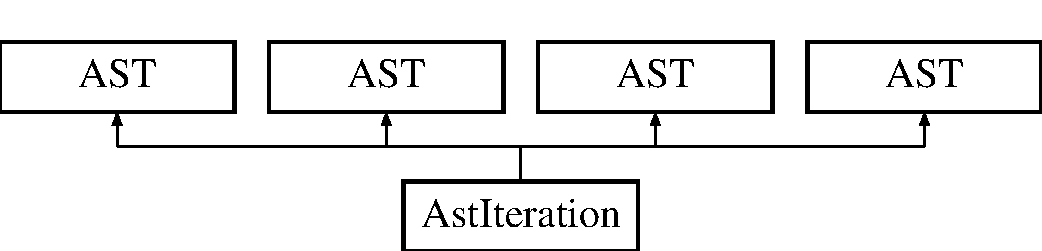
\includegraphics[height=2.000000cm]{classAstIteration}
\end{center}
\end{figure}
\subsection*{Public Types}
\begin{DoxyCompactItemize}
\item 
enum {\bfseries Type} \{ {\bfseries D\-O\-W\-H\-I\-L\-E}, 
{\bfseries W\-H\-I\-L\-E}, 
{\bfseries F\-O\-R}
 \}
\end{DoxyCompactItemize}
\subsection*{Public Member Functions}
\begin{DoxyCompactItemize}
\item 
\hypertarget{classAstIteration_a9b98ddbdb8795a514c129a86fc00b561}{{\bfseries Ast\-Iteration} (\hyperlink{classAstDoWhile}{Ast\-Do\-While} $\ast$d)}\label{classAstIteration_a9b98ddbdb8795a514c129a86fc00b561}

\item 
\hypertarget{classAstIteration_aed79cf13c2e6376cab0a02b657ef6c87}{{\bfseries Ast\-Iteration} (\hyperlink{classAstWhile}{Ast\-While} $\ast$w)}\label{classAstIteration_aed79cf13c2e6376cab0a02b657ef6c87}

\item 
\hypertarget{classAstIteration_a87f1eaa5c3fc5b4562cbad3e54ff5061}{{\bfseries Ast\-Iteration} (\hyperlink{classAstFor}{Ast\-For} $\ast$f)}\label{classAstIteration_a87f1eaa5c3fc5b4562cbad3e54ff5061}

\item 
\hypertarget{classAstIteration_ae3e90f781890621279ff29b5481e0d4b}{void {\bfseries Visit} ()}\label{classAstIteration_ae3e90f781890621279ff29b5481e0d4b}

\item 
\hypertarget{classAST_a71d680856e95ff89f55d5311a552eba6}{void {\bfseries set\-Label} (string l)}\label{classAST_a71d680856e95ff89f55d5311a552eba6}

\item 
\hypertarget{classAST_ab7a5b1d9f1c2de0d98deb356f724a42c}{int {\bfseries get\-U\-I\-D} ()}\label{classAST_ab7a5b1d9f1c2de0d98deb356f724a42c}

\item 
\hypertarget{classAST_aee029be902fffc927d16ccb03eb922ad}{string {\bfseries get\-Label} ()}\label{classAST_aee029be902fffc927d16ccb03eb922ad}

\end{DoxyCompactItemize}
\subsection*{Public Attributes}
\begin{DoxyCompactItemize}
\item 
\hypertarget{classAstIteration_a41e8a7f05a840d8ddd333830f823314c}{enum Ast\-Iteration\-::\-Type {\bfseries t}}\label{classAstIteration_a41e8a7f05a840d8ddd333830f823314c}

\end{DoxyCompactItemize}
\subsection*{Static Public Attributes}
\begin{DoxyCompactItemize}
\item 
\hypertarget{classAST_aca9e6637209b31e03a09c0d42f29bdfa}{static \hyperlink{classVisualizer}{Visualizer} {\bfseries vis}}\label{classAST_aca9e6637209b31e03a09c0d42f29bdfa}

\end{DoxyCompactItemize}
\subsection*{Protected Attributes}
\begin{DoxyCompactItemize}
\item 
\hypertarget{classAST_a847b778f1c3dd5a19de32de432ee6e15}{int {\bfseries uid}}\label{classAST_a847b778f1c3dd5a19de32de432ee6e15}

\item 
\hypertarget{classAST_ab2e239ccc0688d2341724432ff5a1a31}{string {\bfseries label}}\label{classAST_ab2e239ccc0688d2341724432ff5a1a31}

\end{DoxyCompactItemize}
\subsection*{Private Attributes}
\begin{DoxyCompactItemize}
\item 
\hypertarget{classAstIteration_ac984b15a824002ce1825c942271a3020}{\hyperlink{classAstDoWhile}{Ast\-Do\-While} $\ast$ {\bfseries dwl}}\label{classAstIteration_ac984b15a824002ce1825c942271a3020}

\item 
\hypertarget{classAstIteration_aedd1375432ddac3f75b7abe71d7ba34a}{\hyperlink{classAstWhile}{Ast\-While} $\ast$ {\bfseries wl}}\label{classAstIteration_aedd1375432ddac3f75b7abe71d7ba34a}

\item 
\hypertarget{classAstIteration_a166639cd7bfababcd469b182d76be91f}{\hyperlink{classAstFor}{Ast\-For} $\ast$ {\bfseries fr}}\label{classAstIteration_a166639cd7bfababcd469b182d76be91f}

\end{DoxyCompactItemize}


The documentation for this class was generated from the following files\-:\begin{DoxyCompactItemize}
\item 
Ast.\-h\item 
Ast.\-cpp\end{DoxyCompactItemize}

\hypertarget{classAstJump}{\section{Ast\-Jump Class Reference}
\label{classAstJump}\index{Ast\-Jump@{Ast\-Jump}}
}
Inheritance diagram for Ast\-Jump\-:\begin{figure}[H]
\begin{center}
\leavevmode
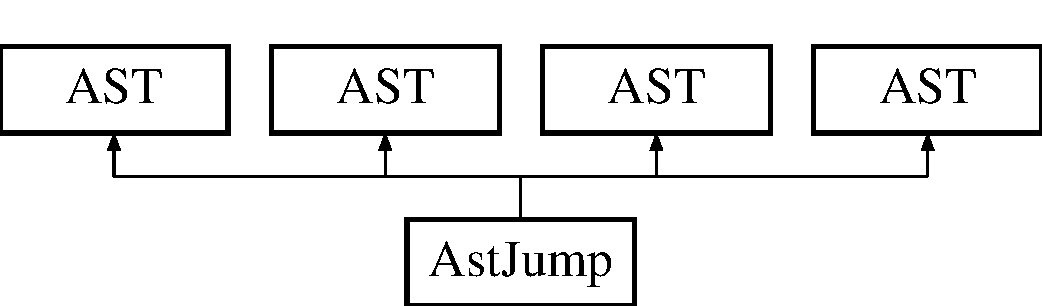
\includegraphics[height=2.000000cm]{classAstJump}
\end{center}
\end{figure}
\subsection*{Public Types}
\begin{DoxyCompactItemize}
\item 
enum {\bfseries Type} \{ \\*
{\bfseries G\-O\-T\-O}, 
{\bfseries C\-O\-N\-T\-I\-N\-U\-E}, 
{\bfseries B\-R\-E\-A\-K}, 
{\bfseries E\-M\-P\-T\-Y\-\_\-\-R\-E\-T\-U\-R\-N}, 
\\*
{\bfseries R\-E\-T\-U\-R\-N}, 
{\bfseries G\-O\-T\-O}, 
{\bfseries C\-O\-N\-T\-I\-N\-U\-E}, 
{\bfseries B\-R\-E\-A\-K}, 
\\*
{\bfseries E\-M\-P\-T\-Y\-\_\-\-R\-E\-T\-U\-R\-N}, 
{\bfseries R\-E\-T\-U\-R\-N}, 
{\bfseries G\-O\-T\-O}, 
{\bfseries C\-O\-N\-T\-I\-N\-U\-E}, 
\\*
{\bfseries B\-R\-E\-A\-K}, 
{\bfseries E\-M\-P\-T\-Y\-\_\-\-R\-E\-T\-U\-R\-N}, 
{\bfseries R\-E\-T\-U\-R\-N}, 
{\bfseries G\-O\-T\-O}, 
\\*
{\bfseries C\-O\-N\-T\-I\-N\-U\-E}, 
{\bfseries B\-R\-E\-A\-K}, 
{\bfseries E\-M\-P\-T\-Y\-\_\-\-R\-E\-T\-U\-R\-N}, 
{\bfseries R\-E\-T\-U\-R\-N}
 \}
\item 
enum {\bfseries Type} \{ \\*
{\bfseries G\-O\-T\-O}, 
{\bfseries C\-O\-N\-T\-I\-N\-U\-E}, 
{\bfseries B\-R\-E\-A\-K}, 
{\bfseries E\-M\-P\-T\-Y\-\_\-\-R\-E\-T\-U\-R\-N}, 
\\*
{\bfseries R\-E\-T\-U\-R\-N}, 
{\bfseries G\-O\-T\-O}, 
{\bfseries C\-O\-N\-T\-I\-N\-U\-E}, 
{\bfseries B\-R\-E\-A\-K}, 
\\*
{\bfseries E\-M\-P\-T\-Y\-\_\-\-R\-E\-T\-U\-R\-N}, 
{\bfseries R\-E\-T\-U\-R\-N}, 
{\bfseries G\-O\-T\-O}, 
{\bfseries C\-O\-N\-T\-I\-N\-U\-E}, 
\\*
{\bfseries B\-R\-E\-A\-K}, 
{\bfseries E\-M\-P\-T\-Y\-\_\-\-R\-E\-T\-U\-R\-N}, 
{\bfseries R\-E\-T\-U\-R\-N}, 
{\bfseries G\-O\-T\-O}, 
\\*
{\bfseries C\-O\-N\-T\-I\-N\-U\-E}, 
{\bfseries B\-R\-E\-A\-K}, 
{\bfseries E\-M\-P\-T\-Y\-\_\-\-R\-E\-T\-U\-R\-N}, 
{\bfseries R\-E\-T\-U\-R\-N}
 \}
\item 
enum {\bfseries Type} \{ \\*
{\bfseries G\-O\-T\-O}, 
{\bfseries C\-O\-N\-T\-I\-N\-U\-E}, 
{\bfseries B\-R\-E\-A\-K}, 
{\bfseries E\-M\-P\-T\-Y\-\_\-\-R\-E\-T\-U\-R\-N}, 
\\*
{\bfseries R\-E\-T\-U\-R\-N}, 
{\bfseries G\-O\-T\-O}, 
{\bfseries C\-O\-N\-T\-I\-N\-U\-E}, 
{\bfseries B\-R\-E\-A\-K}, 
\\*
{\bfseries E\-M\-P\-T\-Y\-\_\-\-R\-E\-T\-U\-R\-N}, 
{\bfseries R\-E\-T\-U\-R\-N}, 
{\bfseries G\-O\-T\-O}, 
{\bfseries C\-O\-N\-T\-I\-N\-U\-E}, 
\\*
{\bfseries B\-R\-E\-A\-K}, 
{\bfseries E\-M\-P\-T\-Y\-\_\-\-R\-E\-T\-U\-R\-N}, 
{\bfseries R\-E\-T\-U\-R\-N}, 
{\bfseries G\-O\-T\-O}, 
\\*
{\bfseries C\-O\-N\-T\-I\-N\-U\-E}, 
{\bfseries B\-R\-E\-A\-K}, 
{\bfseries E\-M\-P\-T\-Y\-\_\-\-R\-E\-T\-U\-R\-N}, 
{\bfseries R\-E\-T\-U\-R\-N}
 \}
\item 
enum {\bfseries Type} \{ \\*
{\bfseries G\-O\-T\-O}, 
{\bfseries C\-O\-N\-T\-I\-N\-U\-E}, 
{\bfseries B\-R\-E\-A\-K}, 
{\bfseries E\-M\-P\-T\-Y\-\_\-\-R\-E\-T\-U\-R\-N}, 
\\*
{\bfseries R\-E\-T\-U\-R\-N}, 
{\bfseries G\-O\-T\-O}, 
{\bfseries C\-O\-N\-T\-I\-N\-U\-E}, 
{\bfseries B\-R\-E\-A\-K}, 
\\*
{\bfseries E\-M\-P\-T\-Y\-\_\-\-R\-E\-T\-U\-R\-N}, 
{\bfseries R\-E\-T\-U\-R\-N}, 
{\bfseries G\-O\-T\-O}, 
{\bfseries C\-O\-N\-T\-I\-N\-U\-E}, 
\\*
{\bfseries B\-R\-E\-A\-K}, 
{\bfseries E\-M\-P\-T\-Y\-\_\-\-R\-E\-T\-U\-R\-N}, 
{\bfseries R\-E\-T\-U\-R\-N}, 
{\bfseries G\-O\-T\-O}, 
\\*
{\bfseries C\-O\-N\-T\-I\-N\-U\-E}, 
{\bfseries B\-R\-E\-A\-K}, 
{\bfseries E\-M\-P\-T\-Y\-\_\-\-R\-E\-T\-U\-R\-N}, 
{\bfseries R\-E\-T\-U\-R\-N}
 \}
\end{DoxyCompactItemize}
\subsection*{Public Member Functions}
\begin{DoxyCompactItemize}
\item 
\hypertarget{classAstJump_a83a4aa905d84f3602374029976d99412}{{\bfseries Ast\-Jump} (\hyperlink{classAstGoto}{Ast\-Goto} $\ast$g, \hyperlink{classAstID}{Ast\-I\-D} $\ast$i)}\label{classAstJump_a83a4aa905d84f3602374029976d99412}

\item 
\hypertarget{classAstJump_a945a1bdc268bfa7f1fdd9f4d39bdef1a}{{\bfseries Ast\-Jump} (\hyperlink{classAstContinue}{Ast\-Continue} $\ast$c)}\label{classAstJump_a945a1bdc268bfa7f1fdd9f4d39bdef1a}

\item 
\hypertarget{classAstJump_a8b9e461b6a974f01889e89728afc7014}{{\bfseries Ast\-Jump} (\hyperlink{classAstBreak}{Ast\-Break} $\ast$b)}\label{classAstJump_a8b9e461b6a974f01889e89728afc7014}

\item 
\hypertarget{classAstJump_a083525b758ad6e931aee5ac850592730}{{\bfseries Ast\-Jump} (\hyperlink{classAstReturn}{Ast\-Return} $\ast$r)}\label{classAstJump_a083525b758ad6e931aee5ac850592730}

\item 
\hypertarget{classAstJump_ad80d35d23849aa369fef153fef4bb99e}{{\bfseries Ast\-Jump} (\hyperlink{classAstReturn}{Ast\-Return} $\ast$r, \hyperlink{classAstExpression}{Ast\-Expression} $\ast$e)}\label{classAstJump_ad80d35d23849aa369fef153fef4bb99e}

\item 
void \hyperlink{classAstJump_aca65cbe034ffdb439f6e3c73e40550ae}{Visit} ()
\begin{DoxyCompactList}\small\item\em This function is responsible for tree traversals. \end{DoxyCompactList}\item 
\hypertarget{classAstJump_a83a4aa905d84f3602374029976d99412}{{\bfseries Ast\-Jump} (\hyperlink{classAstGoto}{Ast\-Goto} $\ast$g, \hyperlink{classAstID}{Ast\-I\-D} $\ast$i)}\label{classAstJump_a83a4aa905d84f3602374029976d99412}

\item 
\hypertarget{classAstJump_a945a1bdc268bfa7f1fdd9f4d39bdef1a}{{\bfseries Ast\-Jump} (\hyperlink{classAstContinue}{Ast\-Continue} $\ast$c)}\label{classAstJump_a945a1bdc268bfa7f1fdd9f4d39bdef1a}

\item 
\hypertarget{classAstJump_a8b9e461b6a974f01889e89728afc7014}{{\bfseries Ast\-Jump} (\hyperlink{classAstBreak}{Ast\-Break} $\ast$b)}\label{classAstJump_a8b9e461b6a974f01889e89728afc7014}

\item 
\hypertarget{classAstJump_a083525b758ad6e931aee5ac850592730}{{\bfseries Ast\-Jump} (\hyperlink{classAstReturn}{Ast\-Return} $\ast$r)}\label{classAstJump_a083525b758ad6e931aee5ac850592730}

\item 
\hypertarget{classAstJump_ad80d35d23849aa369fef153fef4bb99e}{{\bfseries Ast\-Jump} (\hyperlink{classAstReturn}{Ast\-Return} $\ast$r, \hyperlink{classAstExpression}{Ast\-Expression} $\ast$e)}\label{classAstJump_ad80d35d23849aa369fef153fef4bb99e}

\item 
void \hyperlink{classAstJump_aca65cbe034ffdb439f6e3c73e40550ae}{Visit} ()
\begin{DoxyCompactList}\small\item\em This function is responsible for tree traversals. \end{DoxyCompactList}\item 
\hypertarget{classAstJump_a83a4aa905d84f3602374029976d99412}{{\bfseries Ast\-Jump} (\hyperlink{classAstGoto}{Ast\-Goto} $\ast$g, \hyperlink{classAstID}{Ast\-I\-D} $\ast$i)}\label{classAstJump_a83a4aa905d84f3602374029976d99412}

\item 
\hypertarget{classAstJump_a945a1bdc268bfa7f1fdd9f4d39bdef1a}{{\bfseries Ast\-Jump} (\hyperlink{classAstContinue}{Ast\-Continue} $\ast$c)}\label{classAstJump_a945a1bdc268bfa7f1fdd9f4d39bdef1a}

\item 
\hypertarget{classAstJump_a8b9e461b6a974f01889e89728afc7014}{{\bfseries Ast\-Jump} (\hyperlink{classAstBreak}{Ast\-Break} $\ast$b)}\label{classAstJump_a8b9e461b6a974f01889e89728afc7014}

\item 
\hypertarget{classAstJump_a083525b758ad6e931aee5ac850592730}{{\bfseries Ast\-Jump} (\hyperlink{classAstReturn}{Ast\-Return} $\ast$r)}\label{classAstJump_a083525b758ad6e931aee5ac850592730}

\item 
\hypertarget{classAstJump_ad80d35d23849aa369fef153fef4bb99e}{{\bfseries Ast\-Jump} (\hyperlink{classAstReturn}{Ast\-Return} $\ast$r, \hyperlink{classAstExpression}{Ast\-Expression} $\ast$e)}\label{classAstJump_ad80d35d23849aa369fef153fef4bb99e}

\item 
void \hyperlink{classAstJump_aca65cbe034ffdb439f6e3c73e40550ae}{Visit} ()
\begin{DoxyCompactList}\small\item\em This function is responsible for tree traversals. \end{DoxyCompactList}\item 
\hypertarget{classAstJump_a83a4aa905d84f3602374029976d99412}{{\bfseries Ast\-Jump} (\hyperlink{classAstGoto}{Ast\-Goto} $\ast$g, \hyperlink{classAstID}{Ast\-I\-D} $\ast$i)}\label{classAstJump_a83a4aa905d84f3602374029976d99412}

\item 
\hypertarget{classAstJump_a945a1bdc268bfa7f1fdd9f4d39bdef1a}{{\bfseries Ast\-Jump} (\hyperlink{classAstContinue}{Ast\-Continue} $\ast$c)}\label{classAstJump_a945a1bdc268bfa7f1fdd9f4d39bdef1a}

\item 
\hypertarget{classAstJump_a8b9e461b6a974f01889e89728afc7014}{{\bfseries Ast\-Jump} (\hyperlink{classAstBreak}{Ast\-Break} $\ast$b)}\label{classAstJump_a8b9e461b6a974f01889e89728afc7014}

\item 
\hypertarget{classAstJump_a083525b758ad6e931aee5ac850592730}{{\bfseries Ast\-Jump} (\hyperlink{classAstReturn}{Ast\-Return} $\ast$r)}\label{classAstJump_a083525b758ad6e931aee5ac850592730}

\item 
\hypertarget{classAstJump_ad80d35d23849aa369fef153fef4bb99e}{{\bfseries Ast\-Jump} (\hyperlink{classAstReturn}{Ast\-Return} $\ast$r, \hyperlink{classAstExpression}{Ast\-Expression} $\ast$e)}\label{classAstJump_ad80d35d23849aa369fef153fef4bb99e}

\item 
void \hyperlink{classAstJump_aca65cbe034ffdb439f6e3c73e40550ae}{Visit} ()
\begin{DoxyCompactList}\small\item\em This function is responsible for tree traversals. \end{DoxyCompactList}\item 
void \hyperlink{classAST_a71d680856e95ff89f55d5311a552eba6}{set\-Label} (string l)
\begin{DoxyCompactList}\small\item\em Sets the label for the node. \end{DoxyCompactList}\item 
void \hyperlink{classAST_a71d680856e95ff89f55d5311a552eba6}{set\-Label} (string l)
\begin{DoxyCompactList}\small\item\em Sets the label for the node. \end{DoxyCompactList}\item 
void \hyperlink{classAST_a71d680856e95ff89f55d5311a552eba6}{set\-Label} (string l)
\begin{DoxyCompactList}\small\item\em Sets the label for the node. \end{DoxyCompactList}\item 
void \hyperlink{classAST_a71d680856e95ff89f55d5311a552eba6}{set\-Label} (string l)
\begin{DoxyCompactList}\small\item\em Sets the label for the node. \end{DoxyCompactList}\item 
int \hyperlink{classAST_ab7a5b1d9f1c2de0d98deb356f724a42c}{get\-U\-I\-D} ()
\begin{DoxyCompactList}\small\item\em Gets the node's unique I\-D. \end{DoxyCompactList}\item 
int \hyperlink{classAST_ab7a5b1d9f1c2de0d98deb356f724a42c}{get\-U\-I\-D} ()
\begin{DoxyCompactList}\small\item\em Gets the node's unique I\-D. \end{DoxyCompactList}\item 
int \hyperlink{classAST_ab7a5b1d9f1c2de0d98deb356f724a42c}{get\-U\-I\-D} ()
\begin{DoxyCompactList}\small\item\em Gets the node's unique I\-D. \end{DoxyCompactList}\item 
int \hyperlink{classAST_ab7a5b1d9f1c2de0d98deb356f724a42c}{get\-U\-I\-D} ()
\begin{DoxyCompactList}\small\item\em Gets the node's unique I\-D. \end{DoxyCompactList}\item 
string \hyperlink{classAST_aee029be902fffc927d16ccb03eb922ad}{get\-Label} ()
\begin{DoxyCompactList}\small\item\em Gets the node's label. \end{DoxyCompactList}\item 
string \hyperlink{classAST_aee029be902fffc927d16ccb03eb922ad}{get\-Label} ()
\begin{DoxyCompactList}\small\item\em Gets the node's label. \end{DoxyCompactList}\item 
string \hyperlink{classAST_aee029be902fffc927d16ccb03eb922ad}{get\-Label} ()
\begin{DoxyCompactList}\small\item\em Gets the node's label. \end{DoxyCompactList}\item 
string \hyperlink{classAST_aee029be902fffc927d16ccb03eb922ad}{get\-Label} ()
\begin{DoxyCompactList}\small\item\em Gets the node's label. \end{DoxyCompactList}\end{DoxyCompactItemize}
\subsection*{Public Attributes}
\begin{DoxyCompactItemize}
\item 
\hypertarget{classAstJump_a1acc052020f328a4066a8f09c580aa8d}{enum Ast\-Jump\-::\-Type {\bfseries t}}\label{classAstJump_a1acc052020f328a4066a8f09c580aa8d}

\item 
\hypertarget{classAST_aaf215802de409f8096c063d01ffa6783}{bool \hyperlink{classAST_aaf215802de409f8096c063d01ffa6783}{needs\-Cast}}\label{classAST_aaf215802de409f8096c063d01ffa6783}

\begin{DoxyCompactList}\small\item\em This indicates if cast 3\-A\-C needs to be output, and is only relevant for expressions. \end{DoxyCompactList}\item 
\hypertarget{classAST_afa9e77ef650ec6664458fa6cb55be985}{bool \hyperlink{classAST_afa9e77ef650ec6664458fa6cb55be985}{is\-Conv}}\label{classAST_afa9e77ef650ec6664458fa6cb55be985}

\begin{DoxyCompactList}\small\item\em Indicates is a conversion is possible. \end{DoxyCompactList}\item 
\hypertarget{classAST_a61ef3317e023d45237e06615b387cd6b}{C\-O\-N\-V\-E\-R\-S\-I\-O\-N\-T\-Y\-P\-E \hyperlink{classAST_a61ef3317e023d45237e06615b387cd6b}{conv\-Type}}\label{classAST_a61ef3317e023d45237e06615b387cd6b}

\begin{DoxyCompactList}\small\item\em If needs\-Cast is true, then this indicates what the cast should be. \end{DoxyCompactList}\item 
\hypertarget{classAST_aea9b07b39d24183f38c0029cec0a878e}{int \hyperlink{classAST_aea9b07b39d24183f38c0029cec0a878e}{operand\-To\-Cast}}\label{classAST_aea9b07b39d24183f38c0029cec0a878e}

\begin{DoxyCompactList}\small\item\em This indicates if the first or second operand should be the one that is cast. \end{DoxyCompactList}\end{DoxyCompactItemize}
\subsection*{Static Public Attributes}
\begin{DoxyCompactItemize}
\item 
\hypertarget{classAST_a5fdfd5f7b104dd92889163bdadbc68d6}{static \hyperlink{classVisualizer}{Visualizer} \hyperlink{classAST_a5fdfd5f7b104dd92889163bdadbc68d6}{vis}}\label{classAST_a5fdfd5f7b104dd92889163bdadbc68d6}

\begin{DoxyCompactList}\small\item\em Static visualizer instance for generating the visualization of the \hyperlink{classAST}{A\-S\-T}. \end{DoxyCompactList}\item 
\hypertarget{classAST_a8a3ace322f50e030331065d644ee55ee}{static \hyperlink{classTAC__Generator}{T\-A\-C\-\_\-\-Generator} \hyperlink{classAST_a8a3ace322f50e030331065d644ee55ee}{tac\-Gen}}\label{classAST_a8a3ace322f50e030331065d644ee55ee}

\begin{DoxyCompactList}\small\item\em Three address code generator. \end{DoxyCompactList}\item 
\hypertarget{classAST_a1f69448c6dc368d005631a128460083d}{static string {\bfseries current\-Temp} =\char`\"{}\char`\"{}}\label{classAST_a1f69448c6dc368d005631a128460083d}

\item 
\hypertarget{classAST_a551aec090c932ab69365238b40a8a4eb}{static string \hyperlink{classAST_a551aec090c932ab69365238b40a8a4eb}{return\-Label} =\char`\"{}\char`\"{}}\label{classAST_a551aec090c932ab69365238b40a8a4eb}

\begin{DoxyCompactList}\small\item\em This is for storing the string id of any temporary result register that may be created during 3\-A\-C generation. \end{DoxyCompactList}\item 
\hypertarget{classAST_a73c0a266df52be71e6b527b6aa635173}{static list$<$ string $>$ {\bfseries temp\-Stack}}\label{classAST_a73c0a266df52be71e6b527b6aa635173}

\item 
\hypertarget{classAST_abf9e84b541ff04b7bb64e6e4371512d4}{static string {\bfseries last\-I\-D} =\char`\"{}\char`\"{}}\label{classAST_abf9e84b541ff04b7bb64e6e4371512d4}

\item 
\hypertarget{classAST_a163003bfe9c30510ec8039870346049f}{static \hyperlink{classSymTab}{Sym\-Tab} $\ast$ {\bfseries symbol\-Table} =N\-U\-L\-L}\label{classAST_a163003bfe9c30510ec8039870346049f}

\item 
\hypertarget{classAST_a5c3cc894d9c0453523dec9ed76f18a04}{static string {\bfseries current\-Function} =\char`\"{}\char`\"{}}\label{classAST_a5c3cc894d9c0453523dec9ed76f18a04}

\item 
\hypertarget{classAST_a66155513b59ff1a04c8ece8b20ec31f5}{static int {\bfseries current\-Constant\-Value} =0}\label{classAST_a66155513b59ff1a04c8ece8b20ec31f5}

\item 
\hypertarget{classAST_a3d031d7bab635ba1f015aade5943f40c}{static string {\bfseries current\-Id\-Name} =\char`\"{}\char`\"{}}\label{classAST_a3d031d7bab635ba1f015aade5943f40c}

\item 
\hypertarget{classAST_a16c4b6e54febc1a26b31a64a46972ef0}{static int {\bfseries current\-Index\-Val} = 0}\label{classAST_a16c4b6e54febc1a26b31a64a46972ef0}

\end{DoxyCompactItemize}
\subsection*{Protected Attributes}
\begin{DoxyCompactItemize}
\item 
\hypertarget{classAST_a847b778f1c3dd5a19de32de432ee6e15}{int \hyperlink{classAST_a847b778f1c3dd5a19de32de432ee6e15}{uid}}\label{classAST_a847b778f1c3dd5a19de32de432ee6e15}

\begin{DoxyCompactList}\small\item\em The unique id. \end{DoxyCompactList}\item 
\hypertarget{classAST_ab2e239ccc0688d2341724432ff5a1a31}{string \hyperlink{classAST_ab2e239ccc0688d2341724432ff5a1a31}{label}}\label{classAST_ab2e239ccc0688d2341724432ff5a1a31}

\begin{DoxyCompactList}\small\item\em The label to be printed in the visualization. \end{DoxyCompactList}\end{DoxyCompactItemize}
\subsection*{Private Attributes}
\begin{DoxyCompactItemize}
\item 
\hypertarget{classAstJump_aff70d8c8b68050b7e8f8c567562b775c}{\hyperlink{classAstGoto}{Ast\-Goto} $\ast$ {\bfseries go}}\label{classAstJump_aff70d8c8b68050b7e8f8c567562b775c}

\item 
\hypertarget{classAstJump_ac7018c10c9769abc2210eaeec31a04d8}{\hyperlink{classAstID}{Ast\-I\-D} $\ast$ {\bfseries id}}\label{classAstJump_ac7018c10c9769abc2210eaeec31a04d8}

\item 
\hypertarget{classAstJump_a4f424a017e6f34369ae291babe7c4a6e}{\hyperlink{classAstContinue}{Ast\-Continue} $\ast$ {\bfseries cont}}\label{classAstJump_a4f424a017e6f34369ae291babe7c4a6e}

\item 
\hypertarget{classAstJump_a6925dcee97ba433a7b351b04ee7a025a}{\hyperlink{classAstBreak}{Ast\-Break} $\ast$ {\bfseries br}}\label{classAstJump_a6925dcee97ba433a7b351b04ee7a025a}

\item 
\hypertarget{classAstJump_a51021ea2a1fb4411edceb486f07451f5}{\hyperlink{classAstReturn}{Ast\-Return} $\ast$ {\bfseries ret}}\label{classAstJump_a51021ea2a1fb4411edceb486f07451f5}

\item 
\hypertarget{classAstJump_ad7c6e68fd1b542bcd801c955816f81f7}{\hyperlink{classAstExpression}{Ast\-Expression} $\ast$ {\bfseries expr}}\label{classAstJump_ad7c6e68fd1b542bcd801c955816f81f7}

\end{DoxyCompactItemize}


\subsection{Detailed Description}


Definition at line 788 of file Ast.\-h.



\subsection{Member Function Documentation}
\hypertarget{classAST_aee029be902fffc927d16ccb03eb922ad}{\index{Ast\-Jump@{Ast\-Jump}!get\-Label@{get\-Label}}
\index{get\-Label@{get\-Label}!AstJump@{Ast\-Jump}}
\subsubsection[{get\-Label}]{\setlength{\rightskip}{0pt plus 5cm}string A\-S\-T\-::get\-Label (
\begin{DoxyParamCaption}
{}
\end{DoxyParamCaption}
)\hspace{0.3cm}{\ttfamily [inline]}, {\ttfamily [inherited]}}}\label{classAST_aee029be902fffc927d16ccb03eb922ad}


Gets the node's label. 

\begin{DoxyReturn}{Returns}
The label 
\end{DoxyReturn}


Definition at line 60 of file Ast.\-h.

\hypertarget{classAST_aee029be902fffc927d16ccb03eb922ad}{\index{Ast\-Jump@{Ast\-Jump}!get\-Label@{get\-Label}}
\index{get\-Label@{get\-Label}!AstJump@{Ast\-Jump}}
\subsubsection[{get\-Label}]{\setlength{\rightskip}{0pt plus 5cm}string A\-S\-T\-::get\-Label (
\begin{DoxyParamCaption}
{}
\end{DoxyParamCaption}
)\hspace{0.3cm}{\ttfamily [inline]}, {\ttfamily [inherited]}}}\label{classAST_aee029be902fffc927d16ccb03eb922ad}


Gets the node's label. 

\begin{DoxyReturn}{Returns}
The label 
\end{DoxyReturn}


Definition at line 60 of file C\-Scanner.\-ll.

\hypertarget{classAST_aee029be902fffc927d16ccb03eb922ad}{\index{Ast\-Jump@{Ast\-Jump}!get\-Label@{get\-Label}}
\index{get\-Label@{get\-Label}!AstJump@{Ast\-Jump}}
\subsubsection[{get\-Label}]{\setlength{\rightskip}{0pt plus 5cm}string A\-S\-T\-::get\-Label (
\begin{DoxyParamCaption}
{}
\end{DoxyParamCaption}
)\hspace{0.3cm}{\ttfamily [inline]}, {\ttfamily [inherited]}}}\label{classAST_aee029be902fffc927d16ccb03eb922ad}


Gets the node's label. 

\begin{DoxyReturn}{Returns}
The label 
\end{DoxyReturn}


Definition at line 60 of file C\-Parser.\-yy.

\hypertarget{classAST_aee029be902fffc927d16ccb03eb922ad}{\index{Ast\-Jump@{Ast\-Jump}!get\-Label@{get\-Label}}
\index{get\-Label@{get\-Label}!AstJump@{Ast\-Jump}}
\subsubsection[{get\-Label}]{\setlength{\rightskip}{0pt plus 5cm}string A\-S\-T\-::get\-Label (
\begin{DoxyParamCaption}
{}
\end{DoxyParamCaption}
)\hspace{0.3cm}{\ttfamily [inline]}, {\ttfamily [inherited]}}}\label{classAST_aee029be902fffc927d16ccb03eb922ad}


Gets the node's label. 

\begin{DoxyReturn}{Returns}
The label 
\end{DoxyReturn}


Definition at line 60 of file C\-Parser.\-yy.

\hypertarget{classAST_ab7a5b1d9f1c2de0d98deb356f724a42c}{\index{Ast\-Jump@{Ast\-Jump}!get\-U\-I\-D@{get\-U\-I\-D}}
\index{get\-U\-I\-D@{get\-U\-I\-D}!AstJump@{Ast\-Jump}}
\subsubsection[{get\-U\-I\-D}]{\setlength{\rightskip}{0pt plus 5cm}int A\-S\-T\-::get\-U\-I\-D (
\begin{DoxyParamCaption}
{}
\end{DoxyParamCaption}
)\hspace{0.3cm}{\ttfamily [inline]}, {\ttfamily [inherited]}}}\label{classAST_ab7a5b1d9f1c2de0d98deb356f724a42c}


Gets the node's unique I\-D. 

\begin{DoxyReturn}{Returns}
The unique id 
\end{DoxyReturn}


Definition at line 53 of file C\-Parser.\-yy.

\hypertarget{classAST_ab7a5b1d9f1c2de0d98deb356f724a42c}{\index{Ast\-Jump@{Ast\-Jump}!get\-U\-I\-D@{get\-U\-I\-D}}
\index{get\-U\-I\-D@{get\-U\-I\-D}!AstJump@{Ast\-Jump}}
\subsubsection[{get\-U\-I\-D}]{\setlength{\rightskip}{0pt plus 5cm}int A\-S\-T\-::get\-U\-I\-D (
\begin{DoxyParamCaption}
{}
\end{DoxyParamCaption}
)\hspace{0.3cm}{\ttfamily [inline]}, {\ttfamily [inherited]}}}\label{classAST_ab7a5b1d9f1c2de0d98deb356f724a42c}


Gets the node's unique I\-D. 

\begin{DoxyReturn}{Returns}
The unique id 
\end{DoxyReturn}


Definition at line 53 of file C\-Parser.\-yy.

\hypertarget{classAST_ab7a5b1d9f1c2de0d98deb356f724a42c}{\index{Ast\-Jump@{Ast\-Jump}!get\-U\-I\-D@{get\-U\-I\-D}}
\index{get\-U\-I\-D@{get\-U\-I\-D}!AstJump@{Ast\-Jump}}
\subsubsection[{get\-U\-I\-D}]{\setlength{\rightskip}{0pt plus 5cm}int A\-S\-T\-::get\-U\-I\-D (
\begin{DoxyParamCaption}
{}
\end{DoxyParamCaption}
)\hspace{0.3cm}{\ttfamily [inline]}, {\ttfamily [inherited]}}}\label{classAST_ab7a5b1d9f1c2de0d98deb356f724a42c}


Gets the node's unique I\-D. 

\begin{DoxyReturn}{Returns}
The unique id 
\end{DoxyReturn}


Definition at line 53 of file C\-Scanner.\-ll.

\hypertarget{classAST_ab7a5b1d9f1c2de0d98deb356f724a42c}{\index{Ast\-Jump@{Ast\-Jump}!get\-U\-I\-D@{get\-U\-I\-D}}
\index{get\-U\-I\-D@{get\-U\-I\-D}!AstJump@{Ast\-Jump}}
\subsubsection[{get\-U\-I\-D}]{\setlength{\rightskip}{0pt plus 5cm}int A\-S\-T\-::get\-U\-I\-D (
\begin{DoxyParamCaption}
{}
\end{DoxyParamCaption}
)\hspace{0.3cm}{\ttfamily [inline]}, {\ttfamily [inherited]}}}\label{classAST_ab7a5b1d9f1c2de0d98deb356f724a42c}


Gets the node's unique I\-D. 

\begin{DoxyReturn}{Returns}
The unique id 
\end{DoxyReturn}


Definition at line 53 of file Ast.\-h.

\hypertarget{classAST_a71d680856e95ff89f55d5311a552eba6}{\index{Ast\-Jump@{Ast\-Jump}!set\-Label@{set\-Label}}
\index{set\-Label@{set\-Label}!AstJump@{Ast\-Jump}}
\subsubsection[{set\-Label}]{\setlength{\rightskip}{0pt plus 5cm}void A\-S\-T\-::set\-Label (
\begin{DoxyParamCaption}
\item[{string}]{l}
\end{DoxyParamCaption}
)\hspace{0.3cm}{\ttfamily [inline]}, {\ttfamily [inherited]}}}\label{classAST_a71d680856e95ff89f55d5311a552eba6}


Sets the label for the node. 


\begin{DoxyParams}{Parameters}
{\em l} & The label string \\
\hline
\end{DoxyParams}


Definition at line 43 of file C\-Scanner.\-ll.

\hypertarget{classAST_a71d680856e95ff89f55d5311a552eba6}{\index{Ast\-Jump@{Ast\-Jump}!set\-Label@{set\-Label}}
\index{set\-Label@{set\-Label}!AstJump@{Ast\-Jump}}
\subsubsection[{set\-Label}]{\setlength{\rightskip}{0pt plus 5cm}void A\-S\-T\-::set\-Label (
\begin{DoxyParamCaption}
\item[{string}]{l}
\end{DoxyParamCaption}
)\hspace{0.3cm}{\ttfamily [inline]}, {\ttfamily [inherited]}}}\label{classAST_a71d680856e95ff89f55d5311a552eba6}


Sets the label for the node. 


\begin{DoxyParams}{Parameters}
{\em l} & The label string \\
\hline
\end{DoxyParams}


Definition at line 43 of file C\-Parser.\-yy.

\hypertarget{classAST_a71d680856e95ff89f55d5311a552eba6}{\index{Ast\-Jump@{Ast\-Jump}!set\-Label@{set\-Label}}
\index{set\-Label@{set\-Label}!AstJump@{Ast\-Jump}}
\subsubsection[{set\-Label}]{\setlength{\rightskip}{0pt plus 5cm}void A\-S\-T\-::set\-Label (
\begin{DoxyParamCaption}
\item[{string}]{l}
\end{DoxyParamCaption}
)\hspace{0.3cm}{\ttfamily [inline]}, {\ttfamily [inherited]}}}\label{classAST_a71d680856e95ff89f55d5311a552eba6}


Sets the label for the node. 


\begin{DoxyParams}{Parameters}
{\em l} & The label string \\
\hline
\end{DoxyParams}


Definition at line 43 of file Ast.\-h.

\hypertarget{classAST_a71d680856e95ff89f55d5311a552eba6}{\index{Ast\-Jump@{Ast\-Jump}!set\-Label@{set\-Label}}
\index{set\-Label@{set\-Label}!AstJump@{Ast\-Jump}}
\subsubsection[{set\-Label}]{\setlength{\rightskip}{0pt plus 5cm}void A\-S\-T\-::set\-Label (
\begin{DoxyParamCaption}
\item[{string}]{l}
\end{DoxyParamCaption}
)\hspace{0.3cm}{\ttfamily [inline]}, {\ttfamily [inherited]}}}\label{classAST_a71d680856e95ff89f55d5311a552eba6}


Sets the label for the node. 


\begin{DoxyParams}{Parameters}
{\em l} & The label string \\
\hline
\end{DoxyParams}


Definition at line 43 of file C\-Parser.\-yy.

\hypertarget{classAstJump_aca65cbe034ffdb439f6e3c73e40550ae}{\index{Ast\-Jump@{Ast\-Jump}!Visit@{Visit}}
\index{Visit@{Visit}!AstJump@{Ast\-Jump}}
\subsubsection[{Visit}]{\setlength{\rightskip}{0pt plus 5cm}void Ast\-Jump\-::\-Visit (
\begin{DoxyParamCaption}
{}
\end{DoxyParamCaption}
)\hspace{0.3cm}{\ttfamily [virtual]}}}\label{classAstJump_aca65cbe034ffdb439f6e3c73e40550ae}


This function is responsible for tree traversals. 

This function will call the Visit functions of each of it's children nodes, call the visualization code for itself, and output any 3\-A\-C that can be generated at the current node. 

Reimplemented from \hyperlink{classAST_a5828cc86f2c4f1a0aeab6d7069e8fd82}{A\-S\-T}.



Definition at line 2184 of file Ast.\-cpp.

\hypertarget{classAstJump_aca65cbe034ffdb439f6e3c73e40550ae}{\index{Ast\-Jump@{Ast\-Jump}!Visit@{Visit}}
\index{Visit@{Visit}!AstJump@{Ast\-Jump}}
\subsubsection[{Visit}]{\setlength{\rightskip}{0pt plus 5cm}void Ast\-Jump\-::\-Visit (
\begin{DoxyParamCaption}
{}
\end{DoxyParamCaption}
)\hspace{0.3cm}{\ttfamily [virtual]}}}\label{classAstJump_aca65cbe034ffdb439f6e3c73e40550ae}


This function is responsible for tree traversals. 

This function will call the Visit functions of each of it's children nodes, call the visualization code for itself, and output any 3\-A\-C that can be generated at the current node. 

Reimplemented from \hyperlink{classAST_a5828cc86f2c4f1a0aeab6d7069e8fd82}{A\-S\-T}.

\hypertarget{classAstJump_aca65cbe034ffdb439f6e3c73e40550ae}{\index{Ast\-Jump@{Ast\-Jump}!Visit@{Visit}}
\index{Visit@{Visit}!AstJump@{Ast\-Jump}}
\subsubsection[{Visit}]{\setlength{\rightskip}{0pt plus 5cm}void Ast\-Jump\-::\-Visit (
\begin{DoxyParamCaption}
{}
\end{DoxyParamCaption}
)\hspace{0.3cm}{\ttfamily [virtual]}}}\label{classAstJump_aca65cbe034ffdb439f6e3c73e40550ae}


This function is responsible for tree traversals. 

This function will call the Visit functions of each of it's children nodes, call the visualization code for itself, and output any 3\-A\-C that can be generated at the current node. 

Reimplemented from \hyperlink{classAST_a5828cc86f2c4f1a0aeab6d7069e8fd82}{A\-S\-T}.

\hypertarget{classAstJump_aca65cbe034ffdb439f6e3c73e40550ae}{\index{Ast\-Jump@{Ast\-Jump}!Visit@{Visit}}
\index{Visit@{Visit}!AstJump@{Ast\-Jump}}
\subsubsection[{Visit}]{\setlength{\rightskip}{0pt plus 5cm}void Ast\-Jump\-::\-Visit (
\begin{DoxyParamCaption}
{}
\end{DoxyParamCaption}
)\hspace{0.3cm}{\ttfamily [virtual]}}}\label{classAstJump_aca65cbe034ffdb439f6e3c73e40550ae}


This function is responsible for tree traversals. 

This function will call the Visit functions of each of it's children nodes, call the visualization code for itself, and output any 3\-A\-C that can be generated at the current node. 

Reimplemented from \hyperlink{classAST_a5828cc86f2c4f1a0aeab6d7069e8fd82}{A\-S\-T}.



The documentation for this class was generated from the following files\-:\begin{DoxyCompactItemize}
\item 
Ast.\-h\item 
Ast.\-cpp\end{DoxyCompactItemize}

\hypertarget{classAstLabeledStmt}{\section{Ast\-Labeled\-Stmt Class Reference}
\label{classAstLabeledStmt}\index{Ast\-Labeled\-Stmt@{Ast\-Labeled\-Stmt}}
}
Inheritance diagram for Ast\-Labeled\-Stmt\-:\begin{figure}[H]
\begin{center}
\leavevmode
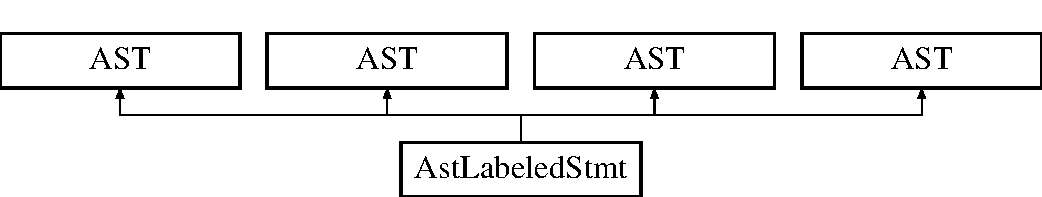
\includegraphics[height=2.000000cm]{classAstLabeledStmt}
\end{center}
\end{figure}
\subsection*{Public Types}
\begin{DoxyCompactItemize}
\item 
enum {\bfseries Type} \{ \\*
{\bfseries N\-O\-\_\-\-C\-A\-S\-E}, 
{\bfseries C\-A\-S\-E}, 
{\bfseries D\-E\-F\-A\-U\-L\-T}, 
{\bfseries N\-O\-\_\-\-C\-A\-S\-E}, 
\\*
{\bfseries C\-A\-S\-E}, 
{\bfseries D\-E\-F\-A\-U\-L\-T}, 
{\bfseries N\-O\-\_\-\-C\-A\-S\-E}, 
{\bfseries C\-A\-S\-E}, 
\\*
{\bfseries D\-E\-F\-A\-U\-L\-T}, 
{\bfseries N\-O\-\_\-\-C\-A\-S\-E}, 
{\bfseries C\-A\-S\-E}, 
{\bfseries D\-E\-F\-A\-U\-L\-T}
 \}
\item 
enum {\bfseries Type} \{ \\*
{\bfseries N\-O\-\_\-\-C\-A\-S\-E}, 
{\bfseries C\-A\-S\-E}, 
{\bfseries D\-E\-F\-A\-U\-L\-T}, 
{\bfseries N\-O\-\_\-\-C\-A\-S\-E}, 
\\*
{\bfseries C\-A\-S\-E}, 
{\bfseries D\-E\-F\-A\-U\-L\-T}, 
{\bfseries N\-O\-\_\-\-C\-A\-S\-E}, 
{\bfseries C\-A\-S\-E}, 
\\*
{\bfseries D\-E\-F\-A\-U\-L\-T}, 
{\bfseries N\-O\-\_\-\-C\-A\-S\-E}, 
{\bfseries C\-A\-S\-E}, 
{\bfseries D\-E\-F\-A\-U\-L\-T}
 \}
\item 
enum {\bfseries Type} \{ \\*
{\bfseries N\-O\-\_\-\-C\-A\-S\-E}, 
{\bfseries C\-A\-S\-E}, 
{\bfseries D\-E\-F\-A\-U\-L\-T}, 
{\bfseries N\-O\-\_\-\-C\-A\-S\-E}, 
\\*
{\bfseries C\-A\-S\-E}, 
{\bfseries D\-E\-F\-A\-U\-L\-T}, 
{\bfseries N\-O\-\_\-\-C\-A\-S\-E}, 
{\bfseries C\-A\-S\-E}, 
\\*
{\bfseries D\-E\-F\-A\-U\-L\-T}, 
{\bfseries N\-O\-\_\-\-C\-A\-S\-E}, 
{\bfseries C\-A\-S\-E}, 
{\bfseries D\-E\-F\-A\-U\-L\-T}
 \}
\item 
enum {\bfseries Type} \{ \\*
{\bfseries N\-O\-\_\-\-C\-A\-S\-E}, 
{\bfseries C\-A\-S\-E}, 
{\bfseries D\-E\-F\-A\-U\-L\-T}, 
{\bfseries N\-O\-\_\-\-C\-A\-S\-E}, 
\\*
{\bfseries C\-A\-S\-E}, 
{\bfseries D\-E\-F\-A\-U\-L\-T}, 
{\bfseries N\-O\-\_\-\-C\-A\-S\-E}, 
{\bfseries C\-A\-S\-E}, 
\\*
{\bfseries D\-E\-F\-A\-U\-L\-T}, 
{\bfseries N\-O\-\_\-\-C\-A\-S\-E}, 
{\bfseries C\-A\-S\-E}, 
{\bfseries D\-E\-F\-A\-U\-L\-T}
 \}
\end{DoxyCompactItemize}
\subsection*{Public Member Functions}
\begin{DoxyCompactItemize}
\item 
\hypertarget{classAstLabeledStmt_aca812c738648cde75efb63b54ea4083d}{{\bfseries Ast\-Labeled\-Stmt} (\hyperlink{classAstID}{Ast\-I\-D} $\ast$i, \hyperlink{classAstStatement}{Ast\-Statement} $\ast$s)}\label{classAstLabeledStmt_aca812c738648cde75efb63b54ea4083d}

\item 
\hypertarget{classAstLabeledStmt_a49285a53627a00f502fa04afb2a72d47}{{\bfseries Ast\-Labeled\-Stmt} (\hyperlink{classAstConstantExpr}{Ast\-Constant\-Expr} $\ast$c, \hyperlink{classAstStatement}{Ast\-Statement} $\ast$s)}\label{classAstLabeledStmt_a49285a53627a00f502fa04afb2a72d47}

\item 
\hypertarget{classAstLabeledStmt_a545ffe76c4ebdc254a554f655b1d19e4}{{\bfseries Ast\-Labeled\-Stmt} (\hyperlink{classAstStatement}{Ast\-Statement} $\ast$s)}\label{classAstLabeledStmt_a545ffe76c4ebdc254a554f655b1d19e4}

\item 
void \hyperlink{classAstLabeledStmt_a2477cd4279ec466452407604e0897261}{Visit} ()
\begin{DoxyCompactList}\small\item\em This function is responsible for tree traversals. \end{DoxyCompactList}\item 
\hypertarget{classAstLabeledStmt_aca812c738648cde75efb63b54ea4083d}{{\bfseries Ast\-Labeled\-Stmt} (\hyperlink{classAstID}{Ast\-I\-D} $\ast$i, \hyperlink{classAstStatement}{Ast\-Statement} $\ast$s)}\label{classAstLabeledStmt_aca812c738648cde75efb63b54ea4083d}

\item 
\hypertarget{classAstLabeledStmt_a49285a53627a00f502fa04afb2a72d47}{{\bfseries Ast\-Labeled\-Stmt} (\hyperlink{classAstConstantExpr}{Ast\-Constant\-Expr} $\ast$c, \hyperlink{classAstStatement}{Ast\-Statement} $\ast$s)}\label{classAstLabeledStmt_a49285a53627a00f502fa04afb2a72d47}

\item 
\hypertarget{classAstLabeledStmt_a545ffe76c4ebdc254a554f655b1d19e4}{{\bfseries Ast\-Labeled\-Stmt} (\hyperlink{classAstStatement}{Ast\-Statement} $\ast$s)}\label{classAstLabeledStmt_a545ffe76c4ebdc254a554f655b1d19e4}

\item 
void \hyperlink{classAstLabeledStmt_a2477cd4279ec466452407604e0897261}{Visit} ()
\begin{DoxyCompactList}\small\item\em This function is responsible for tree traversals. \end{DoxyCompactList}\item 
\hypertarget{classAstLabeledStmt_aca812c738648cde75efb63b54ea4083d}{{\bfseries Ast\-Labeled\-Stmt} (\hyperlink{classAstID}{Ast\-I\-D} $\ast$i, \hyperlink{classAstStatement}{Ast\-Statement} $\ast$s)}\label{classAstLabeledStmt_aca812c738648cde75efb63b54ea4083d}

\item 
\hypertarget{classAstLabeledStmt_a49285a53627a00f502fa04afb2a72d47}{{\bfseries Ast\-Labeled\-Stmt} (\hyperlink{classAstConstantExpr}{Ast\-Constant\-Expr} $\ast$c, \hyperlink{classAstStatement}{Ast\-Statement} $\ast$s)}\label{classAstLabeledStmt_a49285a53627a00f502fa04afb2a72d47}

\item 
\hypertarget{classAstLabeledStmt_a545ffe76c4ebdc254a554f655b1d19e4}{{\bfseries Ast\-Labeled\-Stmt} (\hyperlink{classAstStatement}{Ast\-Statement} $\ast$s)}\label{classAstLabeledStmt_a545ffe76c4ebdc254a554f655b1d19e4}

\item 
void \hyperlink{classAstLabeledStmt_a2477cd4279ec466452407604e0897261}{Visit} ()
\begin{DoxyCompactList}\small\item\em This function is responsible for tree traversals. \end{DoxyCompactList}\item 
\hypertarget{classAstLabeledStmt_aca812c738648cde75efb63b54ea4083d}{{\bfseries Ast\-Labeled\-Stmt} (\hyperlink{classAstID}{Ast\-I\-D} $\ast$i, \hyperlink{classAstStatement}{Ast\-Statement} $\ast$s)}\label{classAstLabeledStmt_aca812c738648cde75efb63b54ea4083d}

\item 
\hypertarget{classAstLabeledStmt_a49285a53627a00f502fa04afb2a72d47}{{\bfseries Ast\-Labeled\-Stmt} (\hyperlink{classAstConstantExpr}{Ast\-Constant\-Expr} $\ast$c, \hyperlink{classAstStatement}{Ast\-Statement} $\ast$s)}\label{classAstLabeledStmt_a49285a53627a00f502fa04afb2a72d47}

\item 
\hypertarget{classAstLabeledStmt_a545ffe76c4ebdc254a554f655b1d19e4}{{\bfseries Ast\-Labeled\-Stmt} (\hyperlink{classAstStatement}{Ast\-Statement} $\ast$s)}\label{classAstLabeledStmt_a545ffe76c4ebdc254a554f655b1d19e4}

\item 
void \hyperlink{classAstLabeledStmt_a2477cd4279ec466452407604e0897261}{Visit} ()
\begin{DoxyCompactList}\small\item\em This function is responsible for tree traversals. \end{DoxyCompactList}\item 
void \hyperlink{classAST_a71d680856e95ff89f55d5311a552eba6}{set\-Label} (string l)
\begin{DoxyCompactList}\small\item\em Sets the label for the node. \end{DoxyCompactList}\item 
void \hyperlink{classAST_a71d680856e95ff89f55d5311a552eba6}{set\-Label} (string l)
\begin{DoxyCompactList}\small\item\em Sets the label for the node. \end{DoxyCompactList}\item 
void \hyperlink{classAST_a71d680856e95ff89f55d5311a552eba6}{set\-Label} (string l)
\begin{DoxyCompactList}\small\item\em Sets the label for the node. \end{DoxyCompactList}\item 
void \hyperlink{classAST_a71d680856e95ff89f55d5311a552eba6}{set\-Label} (string l)
\begin{DoxyCompactList}\small\item\em Sets the label for the node. \end{DoxyCompactList}\item 
int \hyperlink{classAST_ab7a5b1d9f1c2de0d98deb356f724a42c}{get\-U\-I\-D} ()
\begin{DoxyCompactList}\small\item\em Gets the node's unique I\-D. \end{DoxyCompactList}\item 
int \hyperlink{classAST_ab7a5b1d9f1c2de0d98deb356f724a42c}{get\-U\-I\-D} ()
\begin{DoxyCompactList}\small\item\em Gets the node's unique I\-D. \end{DoxyCompactList}\item 
int \hyperlink{classAST_ab7a5b1d9f1c2de0d98deb356f724a42c}{get\-U\-I\-D} ()
\begin{DoxyCompactList}\small\item\em Gets the node's unique I\-D. \end{DoxyCompactList}\item 
int \hyperlink{classAST_ab7a5b1d9f1c2de0d98deb356f724a42c}{get\-U\-I\-D} ()
\begin{DoxyCompactList}\small\item\em Gets the node's unique I\-D. \end{DoxyCompactList}\item 
string \hyperlink{classAST_aee029be902fffc927d16ccb03eb922ad}{get\-Label} ()
\begin{DoxyCompactList}\small\item\em Gets the node's label. \end{DoxyCompactList}\item 
string \hyperlink{classAST_aee029be902fffc927d16ccb03eb922ad}{get\-Label} ()
\begin{DoxyCompactList}\small\item\em Gets the node's label. \end{DoxyCompactList}\item 
string \hyperlink{classAST_aee029be902fffc927d16ccb03eb922ad}{get\-Label} ()
\begin{DoxyCompactList}\small\item\em Gets the node's label. \end{DoxyCompactList}\item 
string \hyperlink{classAST_aee029be902fffc927d16ccb03eb922ad}{get\-Label} ()
\begin{DoxyCompactList}\small\item\em Gets the node's label. \end{DoxyCompactList}\end{DoxyCompactItemize}
\subsection*{Public Attributes}
\begin{DoxyCompactItemize}
\item 
\hypertarget{classAstLabeledStmt_afea3a3521336c57c6fb7bc588a635b1c}{enum Ast\-Labeled\-Stmt\-::\-Type {\bfseries t}}\label{classAstLabeledStmt_afea3a3521336c57c6fb7bc588a635b1c}

\item 
\hypertarget{classAST_aaf215802de409f8096c063d01ffa6783}{bool \hyperlink{classAST_aaf215802de409f8096c063d01ffa6783}{needs\-Cast}}\label{classAST_aaf215802de409f8096c063d01ffa6783}

\begin{DoxyCompactList}\small\item\em This indicates if cast 3\-A\-C needs to be output, and is only relevant for expressions. \end{DoxyCompactList}\item 
\hypertarget{classAST_afa9e77ef650ec6664458fa6cb55be985}{bool \hyperlink{classAST_afa9e77ef650ec6664458fa6cb55be985}{is\-Conv}}\label{classAST_afa9e77ef650ec6664458fa6cb55be985}

\begin{DoxyCompactList}\small\item\em Indicates is a conversion is possible. \end{DoxyCompactList}\item 
\hypertarget{classAST_a61ef3317e023d45237e06615b387cd6b}{C\-O\-N\-V\-E\-R\-S\-I\-O\-N\-T\-Y\-P\-E \hyperlink{classAST_a61ef3317e023d45237e06615b387cd6b}{conv\-Type}}\label{classAST_a61ef3317e023d45237e06615b387cd6b}

\begin{DoxyCompactList}\small\item\em If needs\-Cast is true, then this indicates what the cast should be. \end{DoxyCompactList}\item 
\hypertarget{classAST_aea9b07b39d24183f38c0029cec0a878e}{int \hyperlink{classAST_aea9b07b39d24183f38c0029cec0a878e}{operand\-To\-Cast}}\label{classAST_aea9b07b39d24183f38c0029cec0a878e}

\begin{DoxyCompactList}\small\item\em This indicates if the first or second operand should be the one that is cast. \end{DoxyCompactList}\end{DoxyCompactItemize}
\subsection*{Static Public Attributes}
\begin{DoxyCompactItemize}
\item 
\hypertarget{classAST_a5fdfd5f7b104dd92889163bdadbc68d6}{static \hyperlink{classVisualizer}{Visualizer} \hyperlink{classAST_a5fdfd5f7b104dd92889163bdadbc68d6}{vis}}\label{classAST_a5fdfd5f7b104dd92889163bdadbc68d6}

\begin{DoxyCompactList}\small\item\em Static visualizer instance for generating the visualization of the \hyperlink{classAST}{A\-S\-T}. \end{DoxyCompactList}\item 
\hypertarget{classAST_a8a3ace322f50e030331065d644ee55ee}{static \hyperlink{classTAC__Generator}{T\-A\-C\-\_\-\-Generator} \hyperlink{classAST_a8a3ace322f50e030331065d644ee55ee}{tac\-Gen}}\label{classAST_a8a3ace322f50e030331065d644ee55ee}

\begin{DoxyCompactList}\small\item\em Three address code generator. \end{DoxyCompactList}\item 
\hypertarget{classAST_a1f69448c6dc368d005631a128460083d}{static string {\bfseries current\-Temp} =\char`\"{}\char`\"{}}\label{classAST_a1f69448c6dc368d005631a128460083d}

\item 
\hypertarget{classAST_a551aec090c932ab69365238b40a8a4eb}{static string \hyperlink{classAST_a551aec090c932ab69365238b40a8a4eb}{return\-Label} =\char`\"{}\char`\"{}}\label{classAST_a551aec090c932ab69365238b40a8a4eb}

\begin{DoxyCompactList}\small\item\em This is for storing the string id of any temporary result register that may be created during 3\-A\-C generation. \end{DoxyCompactList}\item 
\hypertarget{classAST_a73c0a266df52be71e6b527b6aa635173}{static list$<$ string $>$ {\bfseries temp\-Stack}}\label{classAST_a73c0a266df52be71e6b527b6aa635173}

\item 
\hypertarget{classAST_abf9e84b541ff04b7bb64e6e4371512d4}{static string {\bfseries last\-I\-D} =\char`\"{}\char`\"{}}\label{classAST_abf9e84b541ff04b7bb64e6e4371512d4}

\item 
\hypertarget{classAST_a163003bfe9c30510ec8039870346049f}{static \hyperlink{classSymTab}{Sym\-Tab} $\ast$ {\bfseries symbol\-Table} =N\-U\-L\-L}\label{classAST_a163003bfe9c30510ec8039870346049f}

\item 
\hypertarget{classAST_a5c3cc894d9c0453523dec9ed76f18a04}{static string {\bfseries current\-Function} =\char`\"{}\char`\"{}}\label{classAST_a5c3cc894d9c0453523dec9ed76f18a04}

\item 
\hypertarget{classAST_a66155513b59ff1a04c8ece8b20ec31f5}{static int {\bfseries current\-Constant\-Value} =0}\label{classAST_a66155513b59ff1a04c8ece8b20ec31f5}

\item 
\hypertarget{classAST_a3d031d7bab635ba1f015aade5943f40c}{static string {\bfseries current\-Id\-Name} =\char`\"{}\char`\"{}}\label{classAST_a3d031d7bab635ba1f015aade5943f40c}

\item 
\hypertarget{classAST_a16c4b6e54febc1a26b31a64a46972ef0}{static int {\bfseries current\-Index\-Val} = 0}\label{classAST_a16c4b6e54febc1a26b31a64a46972ef0}

\item 
\hypertarget{classAST_a6fc65ae9dd064a88941d4b88669b19db}{static string {\bfseries current\-I\-D} = \char`\"{}\char`\"{}}\label{classAST_a6fc65ae9dd064a88941d4b88669b19db}

\end{DoxyCompactItemize}
\subsection*{Protected Attributes}
\begin{DoxyCompactItemize}
\item 
\hypertarget{classAST_a847b778f1c3dd5a19de32de432ee6e15}{int \hyperlink{classAST_a847b778f1c3dd5a19de32de432ee6e15}{uid}}\label{classAST_a847b778f1c3dd5a19de32de432ee6e15}

\begin{DoxyCompactList}\small\item\em The unique id. \end{DoxyCompactList}\item 
\hypertarget{classAST_ab2e239ccc0688d2341724432ff5a1a31}{string \hyperlink{classAST_ab2e239ccc0688d2341724432ff5a1a31}{label}}\label{classAST_ab2e239ccc0688d2341724432ff5a1a31}

\begin{DoxyCompactList}\small\item\em The label to be printed in the visualization. \end{DoxyCompactList}\end{DoxyCompactItemize}
\subsection*{Private Attributes}
\begin{DoxyCompactItemize}
\item 
\hypertarget{classAstLabeledStmt_a121dfefb3b1b463a508d338e98691f4f}{\hyperlink{classAstID}{Ast\-I\-D} $\ast$ {\bfseries id}}\label{classAstLabeledStmt_a121dfefb3b1b463a508d338e98691f4f}

\item 
\hypertarget{classAstLabeledStmt_ac146d1e573fb5423c9968b5150334f7c}{\hyperlink{classAstStatement}{Ast\-Statement} $\ast$ {\bfseries stmt}}\label{classAstLabeledStmt_ac146d1e573fb5423c9968b5150334f7c}

\item 
\hypertarget{classAstLabeledStmt_a6d67cf697a1beb6dd78946fc0c37a379}{\hyperlink{classAstConstantExpr}{Ast\-Constant\-Expr} $\ast$ {\bfseries const\-Expr}}\label{classAstLabeledStmt_a6d67cf697a1beb6dd78946fc0c37a379}

\end{DoxyCompactItemize}


\subsection{Detailed Description}


Definition at line 956 of file Ast.\-h.



\subsection{Member Function Documentation}
\hypertarget{classAST_aee029be902fffc927d16ccb03eb922ad}{\index{Ast\-Labeled\-Stmt@{Ast\-Labeled\-Stmt}!get\-Label@{get\-Label}}
\index{get\-Label@{get\-Label}!AstLabeledStmt@{Ast\-Labeled\-Stmt}}
\subsubsection[{get\-Label}]{\setlength{\rightskip}{0pt plus 5cm}string A\-S\-T\-::get\-Label (
\begin{DoxyParamCaption}
{}
\end{DoxyParamCaption}
)\hspace{0.3cm}{\ttfamily [inline]}, {\ttfamily [inherited]}}}\label{classAST_aee029be902fffc927d16ccb03eb922ad}


Gets the node's label. 

\begin{DoxyReturn}{Returns}
The label 
\end{DoxyReturn}


Definition at line 60 of file Ast.\-h.

\hypertarget{classAST_aee029be902fffc927d16ccb03eb922ad}{\index{Ast\-Labeled\-Stmt@{Ast\-Labeled\-Stmt}!get\-Label@{get\-Label}}
\index{get\-Label@{get\-Label}!AstLabeledStmt@{Ast\-Labeled\-Stmt}}
\subsubsection[{get\-Label}]{\setlength{\rightskip}{0pt plus 5cm}string A\-S\-T\-::get\-Label (
\begin{DoxyParamCaption}
{}
\end{DoxyParamCaption}
)\hspace{0.3cm}{\ttfamily [inline]}, {\ttfamily [inherited]}}}\label{classAST_aee029be902fffc927d16ccb03eb922ad}


Gets the node's label. 

\begin{DoxyReturn}{Returns}
The label 
\end{DoxyReturn}


Definition at line 60 of file C\-Scanner.\-ll.

\hypertarget{classAST_aee029be902fffc927d16ccb03eb922ad}{\index{Ast\-Labeled\-Stmt@{Ast\-Labeled\-Stmt}!get\-Label@{get\-Label}}
\index{get\-Label@{get\-Label}!AstLabeledStmt@{Ast\-Labeled\-Stmt}}
\subsubsection[{get\-Label}]{\setlength{\rightskip}{0pt plus 5cm}string A\-S\-T\-::get\-Label (
\begin{DoxyParamCaption}
{}
\end{DoxyParamCaption}
)\hspace{0.3cm}{\ttfamily [inline]}, {\ttfamily [inherited]}}}\label{classAST_aee029be902fffc927d16ccb03eb922ad}


Gets the node's label. 

\begin{DoxyReturn}{Returns}
The label 
\end{DoxyReturn}


Definition at line 60 of file C\-Parser.\-yy.

\hypertarget{classAST_aee029be902fffc927d16ccb03eb922ad}{\index{Ast\-Labeled\-Stmt@{Ast\-Labeled\-Stmt}!get\-Label@{get\-Label}}
\index{get\-Label@{get\-Label}!AstLabeledStmt@{Ast\-Labeled\-Stmt}}
\subsubsection[{get\-Label}]{\setlength{\rightskip}{0pt plus 5cm}string A\-S\-T\-::get\-Label (
\begin{DoxyParamCaption}
{}
\end{DoxyParamCaption}
)\hspace{0.3cm}{\ttfamily [inline]}, {\ttfamily [inherited]}}}\label{classAST_aee029be902fffc927d16ccb03eb922ad}


Gets the node's label. 

\begin{DoxyReturn}{Returns}
The label 
\end{DoxyReturn}


Definition at line 60 of file C\-Parser.\-yy.

\hypertarget{classAST_ab7a5b1d9f1c2de0d98deb356f724a42c}{\index{Ast\-Labeled\-Stmt@{Ast\-Labeled\-Stmt}!get\-U\-I\-D@{get\-U\-I\-D}}
\index{get\-U\-I\-D@{get\-U\-I\-D}!AstLabeledStmt@{Ast\-Labeled\-Stmt}}
\subsubsection[{get\-U\-I\-D}]{\setlength{\rightskip}{0pt plus 5cm}int A\-S\-T\-::get\-U\-I\-D (
\begin{DoxyParamCaption}
{}
\end{DoxyParamCaption}
)\hspace{0.3cm}{\ttfamily [inline]}, {\ttfamily [inherited]}}}\label{classAST_ab7a5b1d9f1c2de0d98deb356f724a42c}


Gets the node's unique I\-D. 

\begin{DoxyReturn}{Returns}
The unique id 
\end{DoxyReturn}


Definition at line 53 of file C\-Parser.\-yy.

\hypertarget{classAST_ab7a5b1d9f1c2de0d98deb356f724a42c}{\index{Ast\-Labeled\-Stmt@{Ast\-Labeled\-Stmt}!get\-U\-I\-D@{get\-U\-I\-D}}
\index{get\-U\-I\-D@{get\-U\-I\-D}!AstLabeledStmt@{Ast\-Labeled\-Stmt}}
\subsubsection[{get\-U\-I\-D}]{\setlength{\rightskip}{0pt plus 5cm}int A\-S\-T\-::get\-U\-I\-D (
\begin{DoxyParamCaption}
{}
\end{DoxyParamCaption}
)\hspace{0.3cm}{\ttfamily [inline]}, {\ttfamily [inherited]}}}\label{classAST_ab7a5b1d9f1c2de0d98deb356f724a42c}


Gets the node's unique I\-D. 

\begin{DoxyReturn}{Returns}
The unique id 
\end{DoxyReturn}


Definition at line 53 of file C\-Parser.\-yy.

\hypertarget{classAST_ab7a5b1d9f1c2de0d98deb356f724a42c}{\index{Ast\-Labeled\-Stmt@{Ast\-Labeled\-Stmt}!get\-U\-I\-D@{get\-U\-I\-D}}
\index{get\-U\-I\-D@{get\-U\-I\-D}!AstLabeledStmt@{Ast\-Labeled\-Stmt}}
\subsubsection[{get\-U\-I\-D}]{\setlength{\rightskip}{0pt plus 5cm}int A\-S\-T\-::get\-U\-I\-D (
\begin{DoxyParamCaption}
{}
\end{DoxyParamCaption}
)\hspace{0.3cm}{\ttfamily [inline]}, {\ttfamily [inherited]}}}\label{classAST_ab7a5b1d9f1c2de0d98deb356f724a42c}


Gets the node's unique I\-D. 

\begin{DoxyReturn}{Returns}
The unique id 
\end{DoxyReturn}


Definition at line 53 of file C\-Scanner.\-ll.

\hypertarget{classAST_ab7a5b1d9f1c2de0d98deb356f724a42c}{\index{Ast\-Labeled\-Stmt@{Ast\-Labeled\-Stmt}!get\-U\-I\-D@{get\-U\-I\-D}}
\index{get\-U\-I\-D@{get\-U\-I\-D}!AstLabeledStmt@{Ast\-Labeled\-Stmt}}
\subsubsection[{get\-U\-I\-D}]{\setlength{\rightskip}{0pt plus 5cm}int A\-S\-T\-::get\-U\-I\-D (
\begin{DoxyParamCaption}
{}
\end{DoxyParamCaption}
)\hspace{0.3cm}{\ttfamily [inline]}, {\ttfamily [inherited]}}}\label{classAST_ab7a5b1d9f1c2de0d98deb356f724a42c}


Gets the node's unique I\-D. 

\begin{DoxyReturn}{Returns}
The unique id 
\end{DoxyReturn}


Definition at line 53 of file Ast.\-h.

\hypertarget{classAST_a71d680856e95ff89f55d5311a552eba6}{\index{Ast\-Labeled\-Stmt@{Ast\-Labeled\-Stmt}!set\-Label@{set\-Label}}
\index{set\-Label@{set\-Label}!AstLabeledStmt@{Ast\-Labeled\-Stmt}}
\subsubsection[{set\-Label}]{\setlength{\rightskip}{0pt plus 5cm}void A\-S\-T\-::set\-Label (
\begin{DoxyParamCaption}
\item[{string}]{l}
\end{DoxyParamCaption}
)\hspace{0.3cm}{\ttfamily [inline]}, {\ttfamily [inherited]}}}\label{classAST_a71d680856e95ff89f55d5311a552eba6}


Sets the label for the node. 


\begin{DoxyParams}{Parameters}
{\em l} & The label string \\
\hline
\end{DoxyParams}


Definition at line 43 of file C\-Scanner.\-ll.

\hypertarget{classAST_a71d680856e95ff89f55d5311a552eba6}{\index{Ast\-Labeled\-Stmt@{Ast\-Labeled\-Stmt}!set\-Label@{set\-Label}}
\index{set\-Label@{set\-Label}!AstLabeledStmt@{Ast\-Labeled\-Stmt}}
\subsubsection[{set\-Label}]{\setlength{\rightskip}{0pt plus 5cm}void A\-S\-T\-::set\-Label (
\begin{DoxyParamCaption}
\item[{string}]{l}
\end{DoxyParamCaption}
)\hspace{0.3cm}{\ttfamily [inline]}, {\ttfamily [inherited]}}}\label{classAST_a71d680856e95ff89f55d5311a552eba6}


Sets the label for the node. 


\begin{DoxyParams}{Parameters}
{\em l} & The label string \\
\hline
\end{DoxyParams}


Definition at line 43 of file C\-Parser.\-yy.

\hypertarget{classAST_a71d680856e95ff89f55d5311a552eba6}{\index{Ast\-Labeled\-Stmt@{Ast\-Labeled\-Stmt}!set\-Label@{set\-Label}}
\index{set\-Label@{set\-Label}!AstLabeledStmt@{Ast\-Labeled\-Stmt}}
\subsubsection[{set\-Label}]{\setlength{\rightskip}{0pt plus 5cm}void A\-S\-T\-::set\-Label (
\begin{DoxyParamCaption}
\item[{string}]{l}
\end{DoxyParamCaption}
)\hspace{0.3cm}{\ttfamily [inline]}, {\ttfamily [inherited]}}}\label{classAST_a71d680856e95ff89f55d5311a552eba6}


Sets the label for the node. 


\begin{DoxyParams}{Parameters}
{\em l} & The label string \\
\hline
\end{DoxyParams}


Definition at line 43 of file Ast.\-h.

\hypertarget{classAST_a71d680856e95ff89f55d5311a552eba6}{\index{Ast\-Labeled\-Stmt@{Ast\-Labeled\-Stmt}!set\-Label@{set\-Label}}
\index{set\-Label@{set\-Label}!AstLabeledStmt@{Ast\-Labeled\-Stmt}}
\subsubsection[{set\-Label}]{\setlength{\rightskip}{0pt plus 5cm}void A\-S\-T\-::set\-Label (
\begin{DoxyParamCaption}
\item[{string}]{l}
\end{DoxyParamCaption}
)\hspace{0.3cm}{\ttfamily [inline]}, {\ttfamily [inherited]}}}\label{classAST_a71d680856e95ff89f55d5311a552eba6}


Sets the label for the node. 


\begin{DoxyParams}{Parameters}
{\em l} & The label string \\
\hline
\end{DoxyParams}


Definition at line 43 of file C\-Parser.\-yy.

\hypertarget{classAstLabeledStmt_a2477cd4279ec466452407604e0897261}{\index{Ast\-Labeled\-Stmt@{Ast\-Labeled\-Stmt}!Visit@{Visit}}
\index{Visit@{Visit}!AstLabeledStmt@{Ast\-Labeled\-Stmt}}
\subsubsection[{Visit}]{\setlength{\rightskip}{0pt plus 5cm}void Ast\-Labeled\-Stmt\-::\-Visit (
\begin{DoxyParamCaption}
{}
\end{DoxyParamCaption}
)\hspace{0.3cm}{\ttfamily [virtual]}}}\label{classAstLabeledStmt_a2477cd4279ec466452407604e0897261}


This function is responsible for tree traversals. 

This function will call the Visit functions of each of it's children nodes, call the visualization code for itself, and output any 3\-A\-C that can be generated at the current node. 

Reimplemented from \hyperlink{classAST_a5828cc86f2c4f1a0aeab6d7069e8fd82}{A\-S\-T}.



Definition at line 2758 of file Ast.\-cpp.

\hypertarget{classAstLabeledStmt_a2477cd4279ec466452407604e0897261}{\index{Ast\-Labeled\-Stmt@{Ast\-Labeled\-Stmt}!Visit@{Visit}}
\index{Visit@{Visit}!AstLabeledStmt@{Ast\-Labeled\-Stmt}}
\subsubsection[{Visit}]{\setlength{\rightskip}{0pt plus 5cm}void Ast\-Labeled\-Stmt\-::\-Visit (
\begin{DoxyParamCaption}
{}
\end{DoxyParamCaption}
)\hspace{0.3cm}{\ttfamily [virtual]}}}\label{classAstLabeledStmt_a2477cd4279ec466452407604e0897261}


This function is responsible for tree traversals. 

This function will call the Visit functions of each of it's children nodes, call the visualization code for itself, and output any 3\-A\-C that can be generated at the current node. 

Reimplemented from \hyperlink{classAST_a5828cc86f2c4f1a0aeab6d7069e8fd82}{A\-S\-T}.

\hypertarget{classAstLabeledStmt_a2477cd4279ec466452407604e0897261}{\index{Ast\-Labeled\-Stmt@{Ast\-Labeled\-Stmt}!Visit@{Visit}}
\index{Visit@{Visit}!AstLabeledStmt@{Ast\-Labeled\-Stmt}}
\subsubsection[{Visit}]{\setlength{\rightskip}{0pt plus 5cm}void Ast\-Labeled\-Stmt\-::\-Visit (
\begin{DoxyParamCaption}
{}
\end{DoxyParamCaption}
)\hspace{0.3cm}{\ttfamily [virtual]}}}\label{classAstLabeledStmt_a2477cd4279ec466452407604e0897261}


This function is responsible for tree traversals. 

This function will call the Visit functions of each of it's children nodes, call the visualization code for itself, and output any 3\-A\-C that can be generated at the current node. 

Reimplemented from \hyperlink{classAST_a5828cc86f2c4f1a0aeab6d7069e8fd82}{A\-S\-T}.

\hypertarget{classAstLabeledStmt_a2477cd4279ec466452407604e0897261}{\index{Ast\-Labeled\-Stmt@{Ast\-Labeled\-Stmt}!Visit@{Visit}}
\index{Visit@{Visit}!AstLabeledStmt@{Ast\-Labeled\-Stmt}}
\subsubsection[{Visit}]{\setlength{\rightskip}{0pt plus 5cm}void Ast\-Labeled\-Stmt\-::\-Visit (
\begin{DoxyParamCaption}
{}
\end{DoxyParamCaption}
)\hspace{0.3cm}{\ttfamily [virtual]}}}\label{classAstLabeledStmt_a2477cd4279ec466452407604e0897261}


This function is responsible for tree traversals. 

This function will call the Visit functions of each of it's children nodes, call the visualization code for itself, and output any 3\-A\-C that can be generated at the current node. 

Reimplemented from \hyperlink{classAST_a5828cc86f2c4f1a0aeab6d7069e8fd82}{A\-S\-T}.



The documentation for this class was generated from the following files\-:\begin{DoxyCompactItemize}
\item 
Ast.\-h\item 
Ast.\-cpp\end{DoxyCompactItemize}

\hypertarget{classAstLogicAndExpr}{\section{Ast\-Logic\-And\-Expr Class Reference}
\label{classAstLogicAndExpr}\index{Ast\-Logic\-And\-Expr@{Ast\-Logic\-And\-Expr}}
}
Inheritance diagram for Ast\-Logic\-And\-Expr\-:\begin{figure}[H]
\begin{center}
\leavevmode
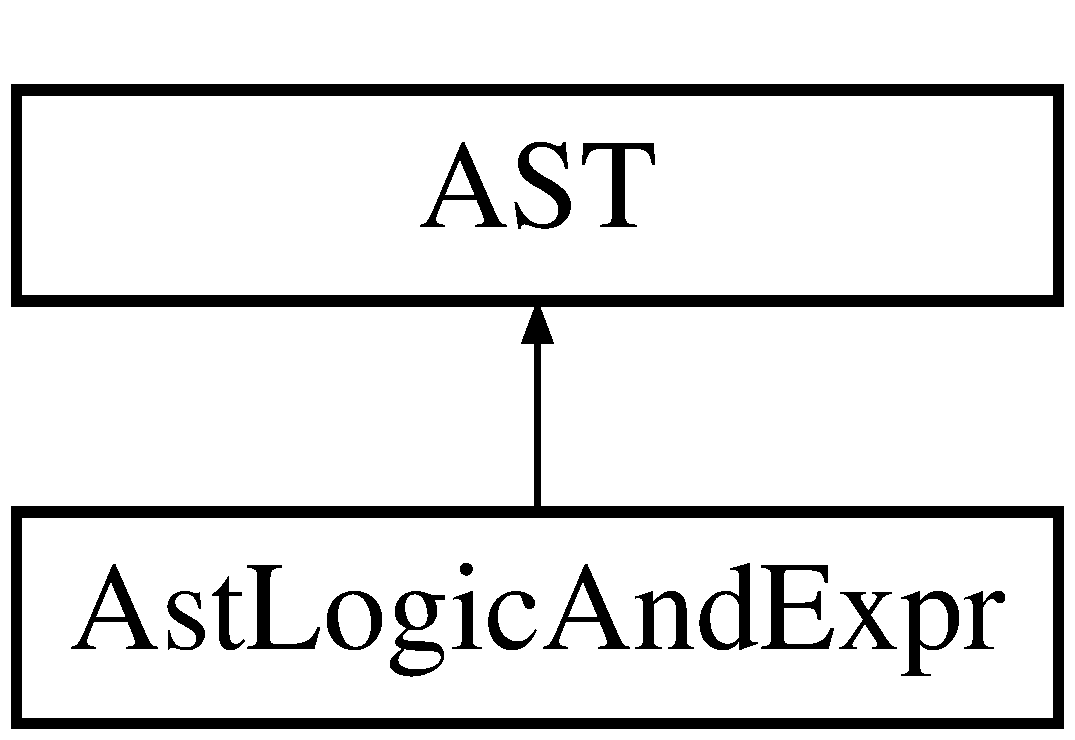
\includegraphics[height=2.000000cm]{classAstLogicAndExpr}
\end{center}
\end{figure}
\subsection*{Public Member Functions}
\begin{DoxyCompactItemize}
\item 
\hypertarget{classAstLogicAndExpr_a7c71466f3ec88e35ac925d7d69fe5e3b}{{\bfseries Ast\-Logic\-And\-Expr} (\hyperlink{classAstORExpr}{Ast\-O\-R\-Expr} $\ast$o)}\label{classAstLogicAndExpr_a7c71466f3ec88e35ac925d7d69fe5e3b}

\item 
\hypertarget{classAstLogicAndExpr_a522ff78d2ca7bf2a3882ad6872b9f1e4}{{\bfseries Ast\-Logic\-And\-Expr} (\hyperlink{classAstLogicAndExpr}{Ast\-Logic\-And\-Expr} $\ast$a, \hyperlink{classAstORExpr}{Ast\-O\-R\-Expr} $\ast$o)}\label{classAstLogicAndExpr_a522ff78d2ca7bf2a3882ad6872b9f1e4}

\item 
void \hyperlink{classAstLogicAndExpr_a4fc66df5e58e7bea73a712986e94ddcf}{Visit} ()
\begin{DoxyCompactList}\small\item\em This function is responsible for tree traversals. \end{DoxyCompactList}\item 
\hypertarget{classAstLogicAndExpr_a7c71466f3ec88e35ac925d7d69fe5e3b}{{\bfseries Ast\-Logic\-And\-Expr} (\hyperlink{classAstORExpr}{Ast\-O\-R\-Expr} $\ast$o)}\label{classAstLogicAndExpr_a7c71466f3ec88e35ac925d7d69fe5e3b}

\item 
\hypertarget{classAstLogicAndExpr_a522ff78d2ca7bf2a3882ad6872b9f1e4}{{\bfseries Ast\-Logic\-And\-Expr} (\hyperlink{classAstLogicAndExpr}{Ast\-Logic\-And\-Expr} $\ast$a, \hyperlink{classAstORExpr}{Ast\-O\-R\-Expr} $\ast$o)}\label{classAstLogicAndExpr_a522ff78d2ca7bf2a3882ad6872b9f1e4}

\item 
void \hyperlink{classAstLogicAndExpr_a4fc66df5e58e7bea73a712986e94ddcf}{Visit} ()
\begin{DoxyCompactList}\small\item\em This function is responsible for tree traversals. \end{DoxyCompactList}\item 
\hypertarget{classAstLogicAndExpr_a7c71466f3ec88e35ac925d7d69fe5e3b}{{\bfseries Ast\-Logic\-And\-Expr} (\hyperlink{classAstORExpr}{Ast\-O\-R\-Expr} $\ast$o)}\label{classAstLogicAndExpr_a7c71466f3ec88e35ac925d7d69fe5e3b}

\item 
\hypertarget{classAstLogicAndExpr_a522ff78d2ca7bf2a3882ad6872b9f1e4}{{\bfseries Ast\-Logic\-And\-Expr} (\hyperlink{classAstLogicAndExpr}{Ast\-Logic\-And\-Expr} $\ast$a, \hyperlink{classAstORExpr}{Ast\-O\-R\-Expr} $\ast$o)}\label{classAstLogicAndExpr_a522ff78d2ca7bf2a3882ad6872b9f1e4}

\item 
void \hyperlink{classAstLogicAndExpr_a4fc66df5e58e7bea73a712986e94ddcf}{Visit} ()
\begin{DoxyCompactList}\small\item\em This function is responsible for tree traversals. \end{DoxyCompactList}\item 
\hypertarget{classAstLogicAndExpr_a7c71466f3ec88e35ac925d7d69fe5e3b}{{\bfseries Ast\-Logic\-And\-Expr} (\hyperlink{classAstORExpr}{Ast\-O\-R\-Expr} $\ast$o)}\label{classAstLogicAndExpr_a7c71466f3ec88e35ac925d7d69fe5e3b}

\item 
\hypertarget{classAstLogicAndExpr_a522ff78d2ca7bf2a3882ad6872b9f1e4}{{\bfseries Ast\-Logic\-And\-Expr} (\hyperlink{classAstLogicAndExpr}{Ast\-Logic\-And\-Expr} $\ast$a, \hyperlink{classAstORExpr}{Ast\-O\-R\-Expr} $\ast$o)}\label{classAstLogicAndExpr_a522ff78d2ca7bf2a3882ad6872b9f1e4}

\item 
void \hyperlink{classAstLogicAndExpr_a4fc66df5e58e7bea73a712986e94ddcf}{Visit} ()
\begin{DoxyCompactList}\small\item\em This function is responsible for tree traversals. \end{DoxyCompactList}\item 
void \hyperlink{classAST_a71d680856e95ff89f55d5311a552eba6}{set\-Label} (string l)
\begin{DoxyCompactList}\small\item\em Sets the label for the node. \end{DoxyCompactList}\item 
void \hyperlink{classAST_a71d680856e95ff89f55d5311a552eba6}{set\-Label} (string l)
\begin{DoxyCompactList}\small\item\em Sets the label for the node. \end{DoxyCompactList}\item 
void \hyperlink{classAST_a71d680856e95ff89f55d5311a552eba6}{set\-Label} (string l)
\begin{DoxyCompactList}\small\item\em Sets the label for the node. \end{DoxyCompactList}\item 
void \hyperlink{classAST_a71d680856e95ff89f55d5311a552eba6}{set\-Label} (string l)
\begin{DoxyCompactList}\small\item\em Sets the label for the node. \end{DoxyCompactList}\item 
int \hyperlink{classAST_ab7a5b1d9f1c2de0d98deb356f724a42c}{get\-U\-I\-D} ()
\begin{DoxyCompactList}\small\item\em Gets the node's unique I\-D. \end{DoxyCompactList}\item 
int \hyperlink{classAST_ab7a5b1d9f1c2de0d98deb356f724a42c}{get\-U\-I\-D} ()
\begin{DoxyCompactList}\small\item\em Gets the node's unique I\-D. \end{DoxyCompactList}\item 
int \hyperlink{classAST_ab7a5b1d9f1c2de0d98deb356f724a42c}{get\-U\-I\-D} ()
\begin{DoxyCompactList}\small\item\em Gets the node's unique I\-D. \end{DoxyCompactList}\item 
int \hyperlink{classAST_ab7a5b1d9f1c2de0d98deb356f724a42c}{get\-U\-I\-D} ()
\begin{DoxyCompactList}\small\item\em Gets the node's unique I\-D. \end{DoxyCompactList}\item 
string \hyperlink{classAST_aee029be902fffc927d16ccb03eb922ad}{get\-Label} ()
\begin{DoxyCompactList}\small\item\em Gets the node's label. \end{DoxyCompactList}\item 
string \hyperlink{classAST_aee029be902fffc927d16ccb03eb922ad}{get\-Label} ()
\begin{DoxyCompactList}\small\item\em Gets the node's label. \end{DoxyCompactList}\item 
string \hyperlink{classAST_aee029be902fffc927d16ccb03eb922ad}{get\-Label} ()
\begin{DoxyCompactList}\small\item\em Gets the node's label. \end{DoxyCompactList}\item 
string \hyperlink{classAST_aee029be902fffc927d16ccb03eb922ad}{get\-Label} ()
\begin{DoxyCompactList}\small\item\em Gets the node's label. \end{DoxyCompactList}\end{DoxyCompactItemize}
\subsection*{Public Attributes}
\begin{DoxyCompactItemize}
\item 
\hypertarget{classAstLogicAndExpr_a1ee89a120e7cef01b084dd24b92cdd68}{\hyperlink{classType}{Type} $\ast$ {\bfseries type}}\label{classAstLogicAndExpr_a1ee89a120e7cef01b084dd24b92cdd68}

\item 
\hypertarget{classAST_aaf215802de409f8096c063d01ffa6783}{bool \hyperlink{classAST_aaf215802de409f8096c063d01ffa6783}{needs\-Cast}}\label{classAST_aaf215802de409f8096c063d01ffa6783}

\begin{DoxyCompactList}\small\item\em This indicates if cast 3\-A\-C needs to be output, and is only relevant for expressions. \end{DoxyCompactList}\item 
\hypertarget{classAST_afa9e77ef650ec6664458fa6cb55be985}{bool \hyperlink{classAST_afa9e77ef650ec6664458fa6cb55be985}{is\-Conv}}\label{classAST_afa9e77ef650ec6664458fa6cb55be985}

\begin{DoxyCompactList}\small\item\em Indicates is a conversion is possible. \end{DoxyCompactList}\item 
\hypertarget{classAST_a61ef3317e023d45237e06615b387cd6b}{C\-O\-N\-V\-E\-R\-S\-I\-O\-N\-T\-Y\-P\-E \hyperlink{classAST_a61ef3317e023d45237e06615b387cd6b}{conv\-Type}}\label{classAST_a61ef3317e023d45237e06615b387cd6b}

\begin{DoxyCompactList}\small\item\em If needs\-Cast is true, then this indicates what the cast should be. \end{DoxyCompactList}\item 
\hypertarget{classAST_aea9b07b39d24183f38c0029cec0a878e}{int \hyperlink{classAST_aea9b07b39d24183f38c0029cec0a878e}{operand\-To\-Cast}}\label{classAST_aea9b07b39d24183f38c0029cec0a878e}

\begin{DoxyCompactList}\small\item\em This indicates if the first or second operand should be the one that is cast. \end{DoxyCompactList}\end{DoxyCompactItemize}
\subsection*{Static Public Attributes}
\begin{DoxyCompactItemize}
\item 
\hypertarget{classAST_a5fdfd5f7b104dd92889163bdadbc68d6}{static \hyperlink{classVisualizer}{Visualizer} \hyperlink{classAST_a5fdfd5f7b104dd92889163bdadbc68d6}{vis}}\label{classAST_a5fdfd5f7b104dd92889163bdadbc68d6}

\begin{DoxyCompactList}\small\item\em Static visualizer instance for generating the visualization of the \hyperlink{classAST}{A\-S\-T}. \end{DoxyCompactList}\item 
\hypertarget{classAST_a8a3ace322f50e030331065d644ee55ee}{static \hyperlink{classTAC__Generator}{T\-A\-C\-\_\-\-Generator} \hyperlink{classAST_a8a3ace322f50e030331065d644ee55ee}{tac\-Gen}}\label{classAST_a8a3ace322f50e030331065d644ee55ee}

\begin{DoxyCompactList}\small\item\em Three address code generator. \end{DoxyCompactList}\item 
\hypertarget{classAST_a1f69448c6dc368d005631a128460083d}{static string {\bfseries current\-Temp} =\char`\"{}\char`\"{}}\label{classAST_a1f69448c6dc368d005631a128460083d}

\item 
\hypertarget{classAST_a551aec090c932ab69365238b40a8a4eb}{static string \hyperlink{classAST_a551aec090c932ab69365238b40a8a4eb}{return\-Label} =\char`\"{}\char`\"{}}\label{classAST_a551aec090c932ab69365238b40a8a4eb}

\begin{DoxyCompactList}\small\item\em This is for storing the string id of any temporary result register that may be created during 3\-A\-C generation. \end{DoxyCompactList}\item 
\hypertarget{classAST_a73c0a266df52be71e6b527b6aa635173}{static list$<$ string $>$ {\bfseries temp\-Stack}}\label{classAST_a73c0a266df52be71e6b527b6aa635173}

\item 
\hypertarget{classAST_abf9e84b541ff04b7bb64e6e4371512d4}{static string {\bfseries last\-I\-D} =\char`\"{}\char`\"{}}\label{classAST_abf9e84b541ff04b7bb64e6e4371512d4}

\item 
\hypertarget{classAST_a163003bfe9c30510ec8039870346049f}{static \hyperlink{classSymTab}{Sym\-Tab} $\ast$ {\bfseries symbol\-Table} =N\-U\-L\-L}\label{classAST_a163003bfe9c30510ec8039870346049f}

\item 
\hypertarget{classAST_a5c3cc894d9c0453523dec9ed76f18a04}{static string {\bfseries current\-Function} =\char`\"{}\char`\"{}}\label{classAST_a5c3cc894d9c0453523dec9ed76f18a04}

\item 
\hypertarget{classAST_a66155513b59ff1a04c8ece8b20ec31f5}{static int {\bfseries current\-Constant\-Value} =0}\label{classAST_a66155513b59ff1a04c8ece8b20ec31f5}

\item 
\hypertarget{classAST_a3d031d7bab635ba1f015aade5943f40c}{static string {\bfseries current\-Id\-Name} =\char`\"{}\char`\"{}}\label{classAST_a3d031d7bab635ba1f015aade5943f40c}

\item 
\hypertarget{classAST_a16c4b6e54febc1a26b31a64a46972ef0}{static int {\bfseries current\-Index\-Val} = 0}\label{classAST_a16c4b6e54febc1a26b31a64a46972ef0}

\item 
\hypertarget{classAST_a6fc65ae9dd064a88941d4b88669b19db}{static string {\bfseries current\-I\-D} = \char`\"{}\char`\"{}}\label{classAST_a6fc65ae9dd064a88941d4b88669b19db}

\end{DoxyCompactItemize}
\subsection*{Protected Attributes}
\begin{DoxyCompactItemize}
\item 
\hypertarget{classAST_a847b778f1c3dd5a19de32de432ee6e15}{int \hyperlink{classAST_a847b778f1c3dd5a19de32de432ee6e15}{uid}}\label{classAST_a847b778f1c3dd5a19de32de432ee6e15}

\begin{DoxyCompactList}\small\item\em The unique id. \end{DoxyCompactList}\item 
\hypertarget{classAST_ab2e239ccc0688d2341724432ff5a1a31}{string \hyperlink{classAST_ab2e239ccc0688d2341724432ff5a1a31}{label}}\label{classAST_ab2e239ccc0688d2341724432ff5a1a31}

\begin{DoxyCompactList}\small\item\em The label to be printed in the visualization. \end{DoxyCompactList}\end{DoxyCompactItemize}
\subsection*{Private Attributes}
\begin{DoxyCompactItemize}
\item 
\hypertarget{classAstLogicAndExpr_a047e943362c7d33c78344b46ad69392c}{\hyperlink{classAstORExpr}{Ast\-O\-R\-Expr} $\ast$ {\bfseries o}}\label{classAstLogicAndExpr_a047e943362c7d33c78344b46ad69392c}

\item 
\hypertarget{classAstLogicAndExpr_a74a88c78a3c3e0d185ceb216f8e979d4}{\hyperlink{classAstLogicAndExpr}{Ast\-Logic\-And\-Expr} $\ast$ {\bfseries a}}\label{classAstLogicAndExpr_a74a88c78a3c3e0d185ceb216f8e979d4}

\end{DoxyCompactItemize}


\subsection{Detailed Description}


Definition at line 670 of file Ast.\-h.



\subsection{Member Function Documentation}
\hypertarget{classAST_aee029be902fffc927d16ccb03eb922ad}{\index{Ast\-Logic\-And\-Expr@{Ast\-Logic\-And\-Expr}!get\-Label@{get\-Label}}
\index{get\-Label@{get\-Label}!AstLogicAndExpr@{Ast\-Logic\-And\-Expr}}
\subsubsection[{get\-Label}]{\setlength{\rightskip}{0pt plus 5cm}string A\-S\-T\-::get\-Label (
\begin{DoxyParamCaption}
{}
\end{DoxyParamCaption}
)\hspace{0.3cm}{\ttfamily [inline]}, {\ttfamily [inherited]}}}\label{classAST_aee029be902fffc927d16ccb03eb922ad}


Gets the node's label. 

\begin{DoxyReturn}{Returns}
The label 
\end{DoxyReturn}


Definition at line 60 of file Ast.\-h.

\hypertarget{classAST_aee029be902fffc927d16ccb03eb922ad}{\index{Ast\-Logic\-And\-Expr@{Ast\-Logic\-And\-Expr}!get\-Label@{get\-Label}}
\index{get\-Label@{get\-Label}!AstLogicAndExpr@{Ast\-Logic\-And\-Expr}}
\subsubsection[{get\-Label}]{\setlength{\rightskip}{0pt plus 5cm}string A\-S\-T\-::get\-Label (
\begin{DoxyParamCaption}
{}
\end{DoxyParamCaption}
)\hspace{0.3cm}{\ttfamily [inline]}, {\ttfamily [inherited]}}}\label{classAST_aee029be902fffc927d16ccb03eb922ad}


Gets the node's label. 

\begin{DoxyReturn}{Returns}
The label 
\end{DoxyReturn}


Definition at line 60 of file C\-Scanner.\-ll.

\hypertarget{classAST_aee029be902fffc927d16ccb03eb922ad}{\index{Ast\-Logic\-And\-Expr@{Ast\-Logic\-And\-Expr}!get\-Label@{get\-Label}}
\index{get\-Label@{get\-Label}!AstLogicAndExpr@{Ast\-Logic\-And\-Expr}}
\subsubsection[{get\-Label}]{\setlength{\rightskip}{0pt plus 5cm}string A\-S\-T\-::get\-Label (
\begin{DoxyParamCaption}
{}
\end{DoxyParamCaption}
)\hspace{0.3cm}{\ttfamily [inline]}, {\ttfamily [inherited]}}}\label{classAST_aee029be902fffc927d16ccb03eb922ad}


Gets the node's label. 

\begin{DoxyReturn}{Returns}
The label 
\end{DoxyReturn}


Definition at line 60 of file C\-Parser.\-yy.

\hypertarget{classAST_aee029be902fffc927d16ccb03eb922ad}{\index{Ast\-Logic\-And\-Expr@{Ast\-Logic\-And\-Expr}!get\-Label@{get\-Label}}
\index{get\-Label@{get\-Label}!AstLogicAndExpr@{Ast\-Logic\-And\-Expr}}
\subsubsection[{get\-Label}]{\setlength{\rightskip}{0pt plus 5cm}string A\-S\-T\-::get\-Label (
\begin{DoxyParamCaption}
{}
\end{DoxyParamCaption}
)\hspace{0.3cm}{\ttfamily [inline]}, {\ttfamily [inherited]}}}\label{classAST_aee029be902fffc927d16ccb03eb922ad}


Gets the node's label. 

\begin{DoxyReturn}{Returns}
The label 
\end{DoxyReturn}


Definition at line 60 of file C\-Parser.\-yy.

\hypertarget{classAST_ab7a5b1d9f1c2de0d98deb356f724a42c}{\index{Ast\-Logic\-And\-Expr@{Ast\-Logic\-And\-Expr}!get\-U\-I\-D@{get\-U\-I\-D}}
\index{get\-U\-I\-D@{get\-U\-I\-D}!AstLogicAndExpr@{Ast\-Logic\-And\-Expr}}
\subsubsection[{get\-U\-I\-D}]{\setlength{\rightskip}{0pt plus 5cm}int A\-S\-T\-::get\-U\-I\-D (
\begin{DoxyParamCaption}
{}
\end{DoxyParamCaption}
)\hspace{0.3cm}{\ttfamily [inline]}, {\ttfamily [inherited]}}}\label{classAST_ab7a5b1d9f1c2de0d98deb356f724a42c}


Gets the node's unique I\-D. 

\begin{DoxyReturn}{Returns}
The unique id 
\end{DoxyReturn}


Definition at line 53 of file C\-Parser.\-yy.

\hypertarget{classAST_ab7a5b1d9f1c2de0d98deb356f724a42c}{\index{Ast\-Logic\-And\-Expr@{Ast\-Logic\-And\-Expr}!get\-U\-I\-D@{get\-U\-I\-D}}
\index{get\-U\-I\-D@{get\-U\-I\-D}!AstLogicAndExpr@{Ast\-Logic\-And\-Expr}}
\subsubsection[{get\-U\-I\-D}]{\setlength{\rightskip}{0pt plus 5cm}int A\-S\-T\-::get\-U\-I\-D (
\begin{DoxyParamCaption}
{}
\end{DoxyParamCaption}
)\hspace{0.3cm}{\ttfamily [inline]}, {\ttfamily [inherited]}}}\label{classAST_ab7a5b1d9f1c2de0d98deb356f724a42c}


Gets the node's unique I\-D. 

\begin{DoxyReturn}{Returns}
The unique id 
\end{DoxyReturn}


Definition at line 53 of file C\-Parser.\-yy.

\hypertarget{classAST_ab7a5b1d9f1c2de0d98deb356f724a42c}{\index{Ast\-Logic\-And\-Expr@{Ast\-Logic\-And\-Expr}!get\-U\-I\-D@{get\-U\-I\-D}}
\index{get\-U\-I\-D@{get\-U\-I\-D}!AstLogicAndExpr@{Ast\-Logic\-And\-Expr}}
\subsubsection[{get\-U\-I\-D}]{\setlength{\rightskip}{0pt plus 5cm}int A\-S\-T\-::get\-U\-I\-D (
\begin{DoxyParamCaption}
{}
\end{DoxyParamCaption}
)\hspace{0.3cm}{\ttfamily [inline]}, {\ttfamily [inherited]}}}\label{classAST_ab7a5b1d9f1c2de0d98deb356f724a42c}


Gets the node's unique I\-D. 

\begin{DoxyReturn}{Returns}
The unique id 
\end{DoxyReturn}


Definition at line 53 of file C\-Scanner.\-ll.

\hypertarget{classAST_ab7a5b1d9f1c2de0d98deb356f724a42c}{\index{Ast\-Logic\-And\-Expr@{Ast\-Logic\-And\-Expr}!get\-U\-I\-D@{get\-U\-I\-D}}
\index{get\-U\-I\-D@{get\-U\-I\-D}!AstLogicAndExpr@{Ast\-Logic\-And\-Expr}}
\subsubsection[{get\-U\-I\-D}]{\setlength{\rightskip}{0pt plus 5cm}int A\-S\-T\-::get\-U\-I\-D (
\begin{DoxyParamCaption}
{}
\end{DoxyParamCaption}
)\hspace{0.3cm}{\ttfamily [inline]}, {\ttfamily [inherited]}}}\label{classAST_ab7a5b1d9f1c2de0d98deb356f724a42c}


Gets the node's unique I\-D. 

\begin{DoxyReturn}{Returns}
The unique id 
\end{DoxyReturn}


Definition at line 53 of file Ast.\-h.

\hypertarget{classAST_a71d680856e95ff89f55d5311a552eba6}{\index{Ast\-Logic\-And\-Expr@{Ast\-Logic\-And\-Expr}!set\-Label@{set\-Label}}
\index{set\-Label@{set\-Label}!AstLogicAndExpr@{Ast\-Logic\-And\-Expr}}
\subsubsection[{set\-Label}]{\setlength{\rightskip}{0pt plus 5cm}void A\-S\-T\-::set\-Label (
\begin{DoxyParamCaption}
\item[{string}]{l}
\end{DoxyParamCaption}
)\hspace{0.3cm}{\ttfamily [inline]}, {\ttfamily [inherited]}}}\label{classAST_a71d680856e95ff89f55d5311a552eba6}


Sets the label for the node. 


\begin{DoxyParams}{Parameters}
{\em l} & The label string \\
\hline
\end{DoxyParams}


Definition at line 43 of file C\-Scanner.\-ll.

\hypertarget{classAST_a71d680856e95ff89f55d5311a552eba6}{\index{Ast\-Logic\-And\-Expr@{Ast\-Logic\-And\-Expr}!set\-Label@{set\-Label}}
\index{set\-Label@{set\-Label}!AstLogicAndExpr@{Ast\-Logic\-And\-Expr}}
\subsubsection[{set\-Label}]{\setlength{\rightskip}{0pt plus 5cm}void A\-S\-T\-::set\-Label (
\begin{DoxyParamCaption}
\item[{string}]{l}
\end{DoxyParamCaption}
)\hspace{0.3cm}{\ttfamily [inline]}, {\ttfamily [inherited]}}}\label{classAST_a71d680856e95ff89f55d5311a552eba6}


Sets the label for the node. 


\begin{DoxyParams}{Parameters}
{\em l} & The label string \\
\hline
\end{DoxyParams}


Definition at line 43 of file C\-Parser.\-yy.

\hypertarget{classAST_a71d680856e95ff89f55d5311a552eba6}{\index{Ast\-Logic\-And\-Expr@{Ast\-Logic\-And\-Expr}!set\-Label@{set\-Label}}
\index{set\-Label@{set\-Label}!AstLogicAndExpr@{Ast\-Logic\-And\-Expr}}
\subsubsection[{set\-Label}]{\setlength{\rightskip}{0pt plus 5cm}void A\-S\-T\-::set\-Label (
\begin{DoxyParamCaption}
\item[{string}]{l}
\end{DoxyParamCaption}
)\hspace{0.3cm}{\ttfamily [inline]}, {\ttfamily [inherited]}}}\label{classAST_a71d680856e95ff89f55d5311a552eba6}


Sets the label for the node. 


\begin{DoxyParams}{Parameters}
{\em l} & The label string \\
\hline
\end{DoxyParams}


Definition at line 43 of file Ast.\-h.

\hypertarget{classAST_a71d680856e95ff89f55d5311a552eba6}{\index{Ast\-Logic\-And\-Expr@{Ast\-Logic\-And\-Expr}!set\-Label@{set\-Label}}
\index{set\-Label@{set\-Label}!AstLogicAndExpr@{Ast\-Logic\-And\-Expr}}
\subsubsection[{set\-Label}]{\setlength{\rightskip}{0pt plus 5cm}void A\-S\-T\-::set\-Label (
\begin{DoxyParamCaption}
\item[{string}]{l}
\end{DoxyParamCaption}
)\hspace{0.3cm}{\ttfamily [inline]}, {\ttfamily [inherited]}}}\label{classAST_a71d680856e95ff89f55d5311a552eba6}


Sets the label for the node. 


\begin{DoxyParams}{Parameters}
{\em l} & The label string \\
\hline
\end{DoxyParams}


Definition at line 43 of file C\-Parser.\-yy.

\hypertarget{classAstLogicAndExpr_a4fc66df5e58e7bea73a712986e94ddcf}{\index{Ast\-Logic\-And\-Expr@{Ast\-Logic\-And\-Expr}!Visit@{Visit}}
\index{Visit@{Visit}!AstLogicAndExpr@{Ast\-Logic\-And\-Expr}}
\subsubsection[{Visit}]{\setlength{\rightskip}{0pt plus 5cm}void Ast\-Logic\-And\-Expr\-::\-Visit (
\begin{DoxyParamCaption}
{}
\end{DoxyParamCaption}
)\hspace{0.3cm}{\ttfamily [virtual]}}}\label{classAstLogicAndExpr_a4fc66df5e58e7bea73a712986e94ddcf}


This function is responsible for tree traversals. 

This function will call the Visit functions of each of it's children nodes, call the visualization code for itself, and output any 3\-A\-C that can be generated at the current node. 

Reimplemented from \hyperlink{classAST_a5828cc86f2c4f1a0aeab6d7069e8fd82}{A\-S\-T}.



Definition at line 1671 of file Ast.\-cpp.

\hypertarget{classAstLogicAndExpr_a4fc66df5e58e7bea73a712986e94ddcf}{\index{Ast\-Logic\-And\-Expr@{Ast\-Logic\-And\-Expr}!Visit@{Visit}}
\index{Visit@{Visit}!AstLogicAndExpr@{Ast\-Logic\-And\-Expr}}
\subsubsection[{Visit}]{\setlength{\rightskip}{0pt plus 5cm}void Ast\-Logic\-And\-Expr\-::\-Visit (
\begin{DoxyParamCaption}
{}
\end{DoxyParamCaption}
)\hspace{0.3cm}{\ttfamily [virtual]}}}\label{classAstLogicAndExpr_a4fc66df5e58e7bea73a712986e94ddcf}


This function is responsible for tree traversals. 

This function will call the Visit functions of each of it's children nodes, call the visualization code for itself, and output any 3\-A\-C that can be generated at the current node. 

Reimplemented from \hyperlink{classAST_a5828cc86f2c4f1a0aeab6d7069e8fd82}{A\-S\-T}.

\hypertarget{classAstLogicAndExpr_a4fc66df5e58e7bea73a712986e94ddcf}{\index{Ast\-Logic\-And\-Expr@{Ast\-Logic\-And\-Expr}!Visit@{Visit}}
\index{Visit@{Visit}!AstLogicAndExpr@{Ast\-Logic\-And\-Expr}}
\subsubsection[{Visit}]{\setlength{\rightskip}{0pt plus 5cm}void Ast\-Logic\-And\-Expr\-::\-Visit (
\begin{DoxyParamCaption}
{}
\end{DoxyParamCaption}
)\hspace{0.3cm}{\ttfamily [virtual]}}}\label{classAstLogicAndExpr_a4fc66df5e58e7bea73a712986e94ddcf}


This function is responsible for tree traversals. 

This function will call the Visit functions of each of it's children nodes, call the visualization code for itself, and output any 3\-A\-C that can be generated at the current node. 

Reimplemented from \hyperlink{classAST_a5828cc86f2c4f1a0aeab6d7069e8fd82}{A\-S\-T}.

\hypertarget{classAstLogicAndExpr_a4fc66df5e58e7bea73a712986e94ddcf}{\index{Ast\-Logic\-And\-Expr@{Ast\-Logic\-And\-Expr}!Visit@{Visit}}
\index{Visit@{Visit}!AstLogicAndExpr@{Ast\-Logic\-And\-Expr}}
\subsubsection[{Visit}]{\setlength{\rightskip}{0pt plus 5cm}void Ast\-Logic\-And\-Expr\-::\-Visit (
\begin{DoxyParamCaption}
{}
\end{DoxyParamCaption}
)\hspace{0.3cm}{\ttfamily [virtual]}}}\label{classAstLogicAndExpr_a4fc66df5e58e7bea73a712986e94ddcf}


This function is responsible for tree traversals. 

This function will call the Visit functions of each of it's children nodes, call the visualization code for itself, and output any 3\-A\-C that can be generated at the current node. 

Reimplemented from \hyperlink{classAST_a5828cc86f2c4f1a0aeab6d7069e8fd82}{A\-S\-T}.



The documentation for this class was generated from the following files\-:\begin{DoxyCompactItemize}
\item 
Ast.\-h\item 
Ast.\-cpp\end{DoxyCompactItemize}

\hypertarget{classAstLogicOrExpr}{\section{Ast\-Logic\-Or\-Expr Class Reference}
\label{classAstLogicOrExpr}\index{Ast\-Logic\-Or\-Expr@{Ast\-Logic\-Or\-Expr}}
}
Inheritance diagram for Ast\-Logic\-Or\-Expr\-:\begin{figure}[H]
\begin{center}
\leavevmode
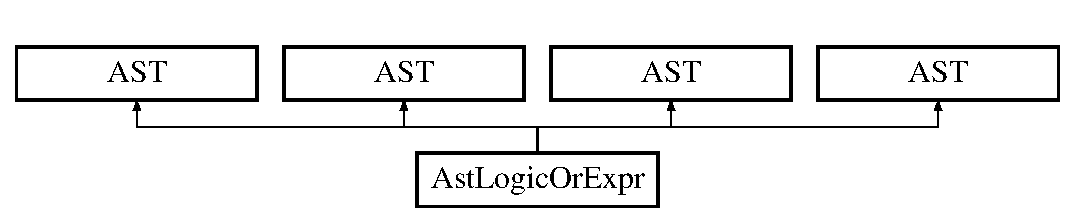
\includegraphics[height=2.000000cm]{classAstLogicOrExpr}
\end{center}
\end{figure}
\subsection*{Public Member Functions}
\begin{DoxyCompactItemize}
\item 
\hypertarget{classAstLogicOrExpr_a9e3103b546a45090ba81ae88fe72b72e}{{\bfseries Ast\-Logic\-Or\-Expr} (\hyperlink{classAstLogicAndExpr}{Ast\-Logic\-And\-Expr} $\ast$a)}\label{classAstLogicOrExpr_a9e3103b546a45090ba81ae88fe72b72e}

\item 
\hypertarget{classAstLogicOrExpr_ade933ad4ec401ffc0dabfb19706fb341}{{\bfseries Ast\-Logic\-Or\-Expr} (\hyperlink{classAstLogicOrExpr}{Ast\-Logic\-Or\-Expr} $\ast$o, \hyperlink{classAstLogicAndExpr}{Ast\-Logic\-And\-Expr} $\ast$a)}\label{classAstLogicOrExpr_ade933ad4ec401ffc0dabfb19706fb341}

\item 
void \hyperlink{classAstLogicOrExpr_acdcdda8eae9c03d8175bbb3527c783eb}{Visit} ()
\begin{DoxyCompactList}\small\item\em This function is responsible for tree traversals. \end{DoxyCompactList}\item 
void \hyperlink{classAST_a71d680856e95ff89f55d5311a552eba6}{set\-Label} (string l)
\begin{DoxyCompactList}\small\item\em Sets the label for the node. \end{DoxyCompactList}\item 
int \hyperlink{classAST_ab7a5b1d9f1c2de0d98deb356f724a42c}{get\-U\-I\-D} ()
\begin{DoxyCompactList}\small\item\em Gets the node's unique I\-D. \end{DoxyCompactList}\item 
string \hyperlink{classAST_aee029be902fffc927d16ccb03eb922ad}{get\-Label} ()
\begin{DoxyCompactList}\small\item\em Gets the node's label. \end{DoxyCompactList}\end{DoxyCompactItemize}
\subsection*{Static Public Attributes}
\begin{DoxyCompactItemize}
\item 
\hypertarget{classAST_aca9e6637209b31e03a09c0d42f29bdfa}{static \hyperlink{classVisualizer}{Visualizer} \hyperlink{classAST_aca9e6637209b31e03a09c0d42f29bdfa}{vis}}\label{classAST_aca9e6637209b31e03a09c0d42f29bdfa}

\begin{DoxyCompactList}\small\item\em Static visualizer instance for generating the visualization of the \hyperlink{classAST}{A\-S\-T}. \end{DoxyCompactList}\end{DoxyCompactItemize}
\subsection*{Protected Attributes}
\begin{DoxyCompactItemize}
\item 
\hypertarget{classAST_a847b778f1c3dd5a19de32de432ee6e15}{int \hyperlink{classAST_a847b778f1c3dd5a19de32de432ee6e15}{uid}}\label{classAST_a847b778f1c3dd5a19de32de432ee6e15}

\begin{DoxyCompactList}\small\item\em The unique id. \end{DoxyCompactList}\item 
\hypertarget{classAST_ab2e239ccc0688d2341724432ff5a1a31}{string \hyperlink{classAST_ab2e239ccc0688d2341724432ff5a1a31}{label}}\label{classAST_ab2e239ccc0688d2341724432ff5a1a31}

\begin{DoxyCompactList}\small\item\em The label to be printed in the visualization. \end{DoxyCompactList}\end{DoxyCompactItemize}
\subsection*{Private Attributes}
\begin{DoxyCompactItemize}
\item 
\hypertarget{classAstLogicOrExpr_a6bfd44db6e0882a6f6cdac1fa98ac2f5}{\hyperlink{classAstLogicAndExpr}{Ast\-Logic\-And\-Expr} $\ast$ {\bfseries a}}\label{classAstLogicOrExpr_a6bfd44db6e0882a6f6cdac1fa98ac2f5}

\item 
\hypertarget{classAstLogicOrExpr_ab5e057f3c286180fc689ad145b9bc2f3}{\hyperlink{classAstLogicOrExpr}{Ast\-Logic\-Or\-Expr} $\ast$ {\bfseries o}}\label{classAstLogicOrExpr_ab5e057f3c286180fc689ad145b9bc2f3}

\end{DoxyCompactItemize}


\subsection{Member Function Documentation}
\hypertarget{classAST_aee029be902fffc927d16ccb03eb922ad}{\index{Ast\-Logic\-Or\-Expr@{Ast\-Logic\-Or\-Expr}!get\-Label@{get\-Label}}
\index{get\-Label@{get\-Label}!AstLogicOrExpr@{Ast\-Logic\-Or\-Expr}}
\subsubsection[{get\-Label}]{\setlength{\rightskip}{0pt plus 5cm}string A\-S\-T\-::get\-Label (
\begin{DoxyParamCaption}
{}
\end{DoxyParamCaption}
)\hspace{0.3cm}{\ttfamily [inline]}, {\ttfamily [inherited]}}}\label{classAST_aee029be902fffc927d16ccb03eb922ad}


Gets the node's label. 

\begin{DoxyReturn}{Returns}
The label 
\end{DoxyReturn}
\hypertarget{classAST_ab7a5b1d9f1c2de0d98deb356f724a42c}{\index{Ast\-Logic\-Or\-Expr@{Ast\-Logic\-Or\-Expr}!get\-U\-I\-D@{get\-U\-I\-D}}
\index{get\-U\-I\-D@{get\-U\-I\-D}!AstLogicOrExpr@{Ast\-Logic\-Or\-Expr}}
\subsubsection[{get\-U\-I\-D}]{\setlength{\rightskip}{0pt plus 5cm}int A\-S\-T\-::get\-U\-I\-D (
\begin{DoxyParamCaption}
{}
\end{DoxyParamCaption}
)\hspace{0.3cm}{\ttfamily [inline]}, {\ttfamily [inherited]}}}\label{classAST_ab7a5b1d9f1c2de0d98deb356f724a42c}


Gets the node's unique I\-D. 

\begin{DoxyReturn}{Returns}
The unique id 
\end{DoxyReturn}
\hypertarget{classAST_a71d680856e95ff89f55d5311a552eba6}{\index{Ast\-Logic\-Or\-Expr@{Ast\-Logic\-Or\-Expr}!set\-Label@{set\-Label}}
\index{set\-Label@{set\-Label}!AstLogicOrExpr@{Ast\-Logic\-Or\-Expr}}
\subsubsection[{set\-Label}]{\setlength{\rightskip}{0pt plus 5cm}void A\-S\-T\-::set\-Label (
\begin{DoxyParamCaption}
\item[{string}]{l}
\end{DoxyParamCaption}
)\hspace{0.3cm}{\ttfamily [inline]}, {\ttfamily [inherited]}}}\label{classAST_a71d680856e95ff89f55d5311a552eba6}


Sets the label for the node. 


\begin{DoxyParams}{Parameters}
{\em l} & The label string \\
\hline
\end{DoxyParams}
\hypertarget{classAstLogicOrExpr_acdcdda8eae9c03d8175bbb3527c783eb}{\index{Ast\-Logic\-Or\-Expr@{Ast\-Logic\-Or\-Expr}!Visit@{Visit}}
\index{Visit@{Visit}!AstLogicOrExpr@{Ast\-Logic\-Or\-Expr}}
\subsubsection[{Visit}]{\setlength{\rightskip}{0pt plus 5cm}void Ast\-Logic\-Or\-Expr\-::\-Visit (
\begin{DoxyParamCaption}
{}
\end{DoxyParamCaption}
)\hspace{0.3cm}{\ttfamily [virtual]}}}\label{classAstLogicOrExpr_acdcdda8eae9c03d8175bbb3527c783eb}


This function is responsible for tree traversals. 

This function will call the Visit functions of each of it's children nodes, call the visualization code for itself, and output any 3\-A\-C that can be generated at the current node. 

Reimplemented from \hyperlink{classAST_a5828cc86f2c4f1a0aeab6d7069e8fd82}{A\-S\-T}.



The documentation for this class was generated from the following files\-:\begin{DoxyCompactItemize}
\item 
Ast.\-h\item 
Ast.\-cpp\end{DoxyCompactItemize}

\hypertarget{classAstMultExpr}{\section{Ast\-Mult\-Expr Class Reference}
\label{classAstMultExpr}\index{Ast\-Mult\-Expr@{Ast\-Mult\-Expr}}
}
Inheritance diagram for Ast\-Mult\-Expr\-:\begin{figure}[H]
\begin{center}
\leavevmode
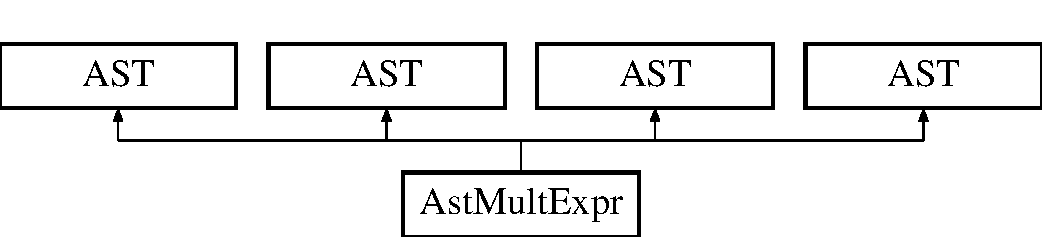
\includegraphics[height=2.000000cm]{classAstMultExpr}
\end{center}
\end{figure}
\subsection*{Public Types}
\begin{DoxyCompactItemize}
\item 
enum {\bfseries Operator} \{ {\bfseries N\-O\-N\-E}, 
{\bfseries S\-T\-A\-R}, 
{\bfseries D\-I\-V}, 
{\bfseries M\-O\-D}
 \}
\end{DoxyCompactItemize}
\subsection*{Public Member Functions}
\begin{DoxyCompactItemize}
\item 
\hypertarget{classAstMultExpr_a5ff1c515cad4ae7084d44d7663a937bc}{{\bfseries Ast\-Mult\-Expr} (\hyperlink{classAstCastExpr}{Ast\-Cast\-Expr} $\ast$c)}\label{classAstMultExpr_a5ff1c515cad4ae7084d44d7663a937bc}

\item 
\hypertarget{classAstMultExpr_a1ef684e47bbad3aa857098807a16ee00}{{\bfseries Ast\-Mult\-Expr} (\hyperlink{classAstMultExpr}{Ast\-Mult\-Expr} $\ast$m, Operator o, \hyperlink{classAstCastExpr}{Ast\-Cast\-Expr} $\ast$c)}\label{classAstMultExpr_a1ef684e47bbad3aa857098807a16ee00}

\item 
\hypertarget{classAstMultExpr_aea6419ae54b97e882c9a9ab79ca73529}{void {\bfseries Visit} ()}\label{classAstMultExpr_aea6419ae54b97e882c9a9ab79ca73529}

\item 
\hypertarget{classAST_a71d680856e95ff89f55d5311a552eba6}{void {\bfseries set\-Label} (string l)}\label{classAST_a71d680856e95ff89f55d5311a552eba6}

\item 
\hypertarget{classAST_ab7a5b1d9f1c2de0d98deb356f724a42c}{int {\bfseries get\-U\-I\-D} ()}\label{classAST_ab7a5b1d9f1c2de0d98deb356f724a42c}

\item 
\hypertarget{classAST_aee029be902fffc927d16ccb03eb922ad}{string {\bfseries get\-Label} ()}\label{classAST_aee029be902fffc927d16ccb03eb922ad}

\end{DoxyCompactItemize}
\subsection*{Public Attributes}
\begin{DoxyCompactItemize}
\item 
\hypertarget{classAstMultExpr_a4a80457ab4cbc7a3b74a9361c3303bc9}{enum Ast\-Mult\-Expr\-::\-Operator {\bfseries op}}\label{classAstMultExpr_a4a80457ab4cbc7a3b74a9361c3303bc9}

\end{DoxyCompactItemize}
\subsection*{Static Public Attributes}
\begin{DoxyCompactItemize}
\item 
\hypertarget{classAST_aca9e6637209b31e03a09c0d42f29bdfa}{static \hyperlink{classVisualizer}{Visualizer} {\bfseries vis}}\label{classAST_aca9e6637209b31e03a09c0d42f29bdfa}

\end{DoxyCompactItemize}
\subsection*{Protected Attributes}
\begin{DoxyCompactItemize}
\item 
\hypertarget{classAST_a847b778f1c3dd5a19de32de432ee6e15}{int {\bfseries uid}}\label{classAST_a847b778f1c3dd5a19de32de432ee6e15}

\item 
\hypertarget{classAST_ab2e239ccc0688d2341724432ff5a1a31}{string {\bfseries label}}\label{classAST_ab2e239ccc0688d2341724432ff5a1a31}

\end{DoxyCompactItemize}
\subsection*{Private Attributes}
\begin{DoxyCompactItemize}
\item 
\hypertarget{classAstMultExpr_a880ddc32727181bc1d8cce71a3fb6f76}{\hyperlink{classAstCastExpr}{Ast\-Cast\-Expr} $\ast$ {\bfseries cast}}\label{classAstMultExpr_a880ddc32727181bc1d8cce71a3fb6f76}

\item 
\hypertarget{classAstMultExpr_a94749396ed57a7d86113c9a198e9560d}{\hyperlink{classAstMultExpr}{Ast\-Mult\-Expr} $\ast$ {\bfseries mult}}\label{classAstMultExpr_a94749396ed57a7d86113c9a198e9560d}

\end{DoxyCompactItemize}


The documentation for this class was generated from the following files\-:\begin{DoxyCompactItemize}
\item 
Ast.\-h\item 
Ast.\-cpp\end{DoxyCompactItemize}

\hypertarget{classAstORExpr}{\section{Ast\-O\-R\-Expr Class Reference}
\label{classAstORExpr}\index{Ast\-O\-R\-Expr@{Ast\-O\-R\-Expr}}
}
Inheritance diagram for Ast\-O\-R\-Expr\-:\begin{figure}[H]
\begin{center}
\leavevmode
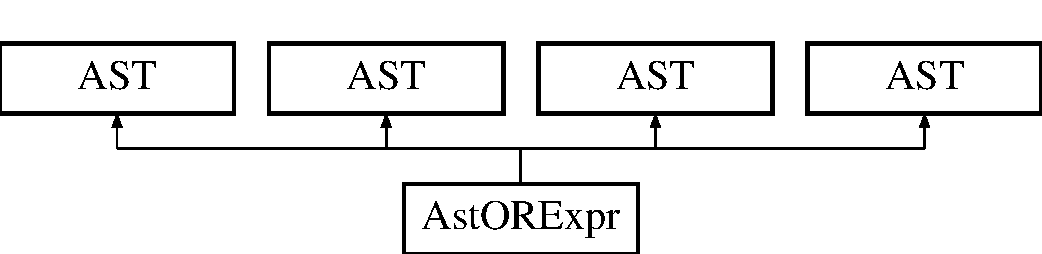
\includegraphics[height=2.000000cm]{classAstORExpr}
\end{center}
\end{figure}
\subsection*{Public Member Functions}
\begin{DoxyCompactItemize}
\item 
\hypertarget{classAstORExpr_a7e7557c1813587fa1a442cb7b5c5317c}{{\bfseries Ast\-O\-R\-Expr} (\hyperlink{classAstXORExpr}{Ast\-X\-O\-R\-Expr} $\ast$x)}\label{classAstORExpr_a7e7557c1813587fa1a442cb7b5c5317c}

\item 
\hypertarget{classAstORExpr_a928d0f31c99cd5d9eef962544465df7e}{{\bfseries Ast\-O\-R\-Expr} (\hyperlink{classAstORExpr}{Ast\-O\-R\-Expr} $\ast$o, \hyperlink{classAstXORExpr}{Ast\-X\-O\-R\-Expr} $\ast$x)}\label{classAstORExpr_a928d0f31c99cd5d9eef962544465df7e}

\item 
void \hyperlink{classAstORExpr_ac442067b01450413dca857727b3af8b3}{Visit} ()
\begin{DoxyCompactList}\small\item\em This function is responsible for tree traversals. \end{DoxyCompactList}\item 
void \hyperlink{classAST_a71d680856e95ff89f55d5311a552eba6}{set\-Label} (string l)
\begin{DoxyCompactList}\small\item\em Sets the label for the node. \end{DoxyCompactList}\item 
int \hyperlink{classAST_ab7a5b1d9f1c2de0d98deb356f724a42c}{get\-U\-I\-D} ()
\begin{DoxyCompactList}\small\item\em Gets the node's unique I\-D. \end{DoxyCompactList}\item 
string \hyperlink{classAST_aee029be902fffc927d16ccb03eb922ad}{get\-Label} ()
\begin{DoxyCompactList}\small\item\em Gets the node's label. \end{DoxyCompactList}\end{DoxyCompactItemize}
\subsection*{Static Public Attributes}
\begin{DoxyCompactItemize}
\item 
\hypertarget{classAST_aca9e6637209b31e03a09c0d42f29bdfa}{static \hyperlink{classVisualizer}{Visualizer} \hyperlink{classAST_aca9e6637209b31e03a09c0d42f29bdfa}{vis}}\label{classAST_aca9e6637209b31e03a09c0d42f29bdfa}

\begin{DoxyCompactList}\small\item\em Static visualizer instance for generating the visualization of the \hyperlink{classAST}{A\-S\-T}. \end{DoxyCompactList}\end{DoxyCompactItemize}
\subsection*{Protected Attributes}
\begin{DoxyCompactItemize}
\item 
\hypertarget{classAST_a847b778f1c3dd5a19de32de432ee6e15}{int \hyperlink{classAST_a847b778f1c3dd5a19de32de432ee6e15}{uid}}\label{classAST_a847b778f1c3dd5a19de32de432ee6e15}

\begin{DoxyCompactList}\small\item\em The unique id. \end{DoxyCompactList}\item 
\hypertarget{classAST_ab2e239ccc0688d2341724432ff5a1a31}{string \hyperlink{classAST_ab2e239ccc0688d2341724432ff5a1a31}{label}}\label{classAST_ab2e239ccc0688d2341724432ff5a1a31}

\begin{DoxyCompactList}\small\item\em The label to be printed in the visualization. \end{DoxyCompactList}\end{DoxyCompactItemize}
\subsection*{Private Attributes}
\begin{DoxyCompactItemize}
\item 
\hypertarget{classAstORExpr_a48febfda9238b0c72ba8193a6cdb3b91}{\hyperlink{classAstXORExpr}{Ast\-X\-O\-R\-Expr} $\ast$ {\bfseries x}}\label{classAstORExpr_a48febfda9238b0c72ba8193a6cdb3b91}

\item 
\hypertarget{classAstORExpr_a1ba5315c8b880fe7c658cb458cd9c54c}{\hyperlink{classAstORExpr}{Ast\-O\-R\-Expr} $\ast$ {\bfseries o}}\label{classAstORExpr_a1ba5315c8b880fe7c658cb458cd9c54c}

\end{DoxyCompactItemize}


\subsection{Member Function Documentation}
\hypertarget{classAST_aee029be902fffc927d16ccb03eb922ad}{\index{Ast\-O\-R\-Expr@{Ast\-O\-R\-Expr}!get\-Label@{get\-Label}}
\index{get\-Label@{get\-Label}!AstORExpr@{Ast\-O\-R\-Expr}}
\subsubsection[{get\-Label}]{\setlength{\rightskip}{0pt plus 5cm}string A\-S\-T\-::get\-Label (
\begin{DoxyParamCaption}
{}
\end{DoxyParamCaption}
)\hspace{0.3cm}{\ttfamily [inline]}, {\ttfamily [inherited]}}}\label{classAST_aee029be902fffc927d16ccb03eb922ad}


Gets the node's label. 

\begin{DoxyReturn}{Returns}
The label 
\end{DoxyReturn}
\hypertarget{classAST_ab7a5b1d9f1c2de0d98deb356f724a42c}{\index{Ast\-O\-R\-Expr@{Ast\-O\-R\-Expr}!get\-U\-I\-D@{get\-U\-I\-D}}
\index{get\-U\-I\-D@{get\-U\-I\-D}!AstORExpr@{Ast\-O\-R\-Expr}}
\subsubsection[{get\-U\-I\-D}]{\setlength{\rightskip}{0pt plus 5cm}int A\-S\-T\-::get\-U\-I\-D (
\begin{DoxyParamCaption}
{}
\end{DoxyParamCaption}
)\hspace{0.3cm}{\ttfamily [inline]}, {\ttfamily [inherited]}}}\label{classAST_ab7a5b1d9f1c2de0d98deb356f724a42c}


Gets the node's unique I\-D. 

\begin{DoxyReturn}{Returns}
The unique id 
\end{DoxyReturn}
\hypertarget{classAST_a71d680856e95ff89f55d5311a552eba6}{\index{Ast\-O\-R\-Expr@{Ast\-O\-R\-Expr}!set\-Label@{set\-Label}}
\index{set\-Label@{set\-Label}!AstORExpr@{Ast\-O\-R\-Expr}}
\subsubsection[{set\-Label}]{\setlength{\rightskip}{0pt plus 5cm}void A\-S\-T\-::set\-Label (
\begin{DoxyParamCaption}
\item[{string}]{l}
\end{DoxyParamCaption}
)\hspace{0.3cm}{\ttfamily [inline]}, {\ttfamily [inherited]}}}\label{classAST_a71d680856e95ff89f55d5311a552eba6}


Sets the label for the node. 


\begin{DoxyParams}{Parameters}
{\em l} & The label string \\
\hline
\end{DoxyParams}
\hypertarget{classAstORExpr_ac442067b01450413dca857727b3af8b3}{\index{Ast\-O\-R\-Expr@{Ast\-O\-R\-Expr}!Visit@{Visit}}
\index{Visit@{Visit}!AstORExpr@{Ast\-O\-R\-Expr}}
\subsubsection[{Visit}]{\setlength{\rightskip}{0pt plus 5cm}void Ast\-O\-R\-Expr\-::\-Visit (
\begin{DoxyParamCaption}
{}
\end{DoxyParamCaption}
)\hspace{0.3cm}{\ttfamily [virtual]}}}\label{classAstORExpr_ac442067b01450413dca857727b3af8b3}


This function is responsible for tree traversals. 

This function will call the Visit functions of each of it's children nodes, call the visualization code for itself, and output any 3\-A\-C that can be generated at the current node. 

Reimplemented from \hyperlink{classAST_a5828cc86f2c4f1a0aeab6d7069e8fd82}{A\-S\-T}.



The documentation for this class was generated from the following files\-:\begin{DoxyCompactItemize}
\item 
Ast.\-h\item 
Ast.\-cpp\end{DoxyCompactItemize}

\input{classAstParamDec}
\input{classAstParamList}
\input{classAstPointer}
\hypertarget{classAstPostfixExpr}{\section{Ast\-Postfix\-Expr Class Reference}
\label{classAstPostfixExpr}\index{Ast\-Postfix\-Expr@{Ast\-Postfix\-Expr}}
}
Inheritance diagram for Ast\-Postfix\-Expr\-:\begin{figure}[H]
\begin{center}
\leavevmode
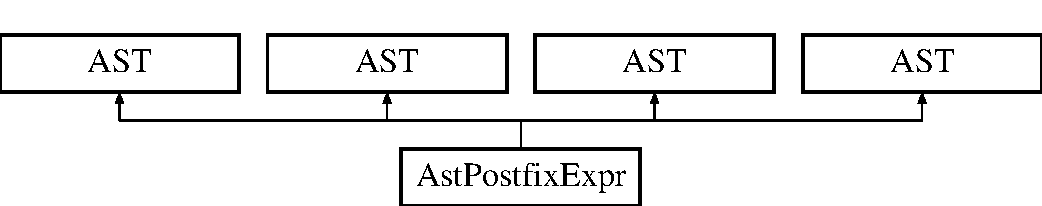
\includegraphics[height=2.000000cm]{classAstPostfixExpr}
\end{center}
\end{figure}
\subsection*{Public Types}
\begin{DoxyCompactItemize}
\item 
enum {\bfseries Operator} \{ \\*
{\bfseries N\-O\-N\-E}, 
{\bfseries D\-O\-T\-\_\-\-O\-P}, 
{\bfseries P\-T\-R\-\_\-\-O\-P}, 
{\bfseries I\-N\-C\-\_\-\-O\-P}, 
\\*
{\bfseries D\-E\-C\-\_\-\-O\-P}
 \}
\item 
enum {\bfseries Type} \{ \\*
{\bfseries P\-R\-I\-M\-A\-R\-Y}, 
{\bfseries B\-R\-A\-C\-K\-E\-T\-S}, 
{\bfseries E\-M\-P\-T\-Y\-\_\-\-P\-A\-R\-E\-N\-S}, 
{\bfseries P\-A\-R\-E\-N\-S}, 
\\*
{\bfseries D\-O\-T}, 
{\bfseries P\-T\-R}, 
{\bfseries I\-N\-C}, 
{\bfseries D\-E\-C}
 \}
\end{DoxyCompactItemize}
\subsection*{Public Member Functions}
\begin{DoxyCompactItemize}
\item 
\hypertarget{classAstPostfixExpr_a8299517f87239b0428545cdfc96f0bbc}{{\bfseries Ast\-Postfix\-Expr} (\hyperlink{classAstPrimaryExpr}{Ast\-Primary\-Expr} $\ast$p)}\label{classAstPostfixExpr_a8299517f87239b0428545cdfc96f0bbc}

\item 
\hypertarget{classAstPostfixExpr_a5dd762cbae8160f94a661ecdf3a90770}{{\bfseries Ast\-Postfix\-Expr} (\hyperlink{classAstPostfixExpr}{Ast\-Postfix\-Expr} $\ast$p, \hyperlink{classAstExpression}{Ast\-Expression} $\ast$e)}\label{classAstPostfixExpr_a5dd762cbae8160f94a661ecdf3a90770}

\item 
\hypertarget{classAstPostfixExpr_af17b325f38a7138728773d86a9342105}{{\bfseries Ast\-Postfix\-Expr} (\hyperlink{classAstPostfixExpr}{Ast\-Postfix\-Expr} $\ast$p)}\label{classAstPostfixExpr_af17b325f38a7138728773d86a9342105}

\item 
\hypertarget{classAstPostfixExpr_a4a1ae7a03b7b29e6641f47479e58aa3b}{{\bfseries Ast\-Postfix\-Expr} (\hyperlink{classAstPostfixExpr}{Ast\-Postfix\-Expr} $\ast$p, \hyperlink{classAstArgExprList}{Ast\-Arg\-Expr\-List} $\ast$a)}\label{classAstPostfixExpr_a4a1ae7a03b7b29e6641f47479e58aa3b}

\item 
\hypertarget{classAstPostfixExpr_a094735e6e2f593a42cc2b9aabc44213b}{{\bfseries Ast\-Postfix\-Expr} (\hyperlink{classAstPostfixExpr}{Ast\-Postfix\-Expr} $\ast$p, Operator o, \hyperlink{classAstID}{Ast\-I\-D} $\ast$i)}\label{classAstPostfixExpr_a094735e6e2f593a42cc2b9aabc44213b}

\item 
\hypertarget{classAstPostfixExpr_a71f3baa5264259031d95741e65de1e07}{{\bfseries Ast\-Postfix\-Expr} (\hyperlink{classAstPostfixExpr}{Ast\-Postfix\-Expr} $\ast$p, Operator o)}\label{classAstPostfixExpr_a71f3baa5264259031d95741e65de1e07}

\item 
void \hyperlink{classAstPostfixExpr_ae3e7fdbd4c2bf888ee62760e6f422cad}{Visit} ()
\begin{DoxyCompactList}\small\item\em This function is responsible for tree traversals. \end{DoxyCompactList}\item 
void \hyperlink{classAST_a71d680856e95ff89f55d5311a552eba6}{set\-Label} (string l)
\begin{DoxyCompactList}\small\item\em Sets the label for the node. \end{DoxyCompactList}\item 
int \hyperlink{classAST_ab7a5b1d9f1c2de0d98deb356f724a42c}{get\-U\-I\-D} ()
\begin{DoxyCompactList}\small\item\em Gets the node's unique I\-D. \end{DoxyCompactList}\item 
string \hyperlink{classAST_aee029be902fffc927d16ccb03eb922ad}{get\-Label} ()
\begin{DoxyCompactList}\small\item\em Gets the node's label. \end{DoxyCompactList}\end{DoxyCompactItemize}
\subsection*{Static Public Attributes}
\begin{DoxyCompactItemize}
\item 
\hypertarget{classAST_aca9e6637209b31e03a09c0d42f29bdfa}{static \hyperlink{classVisualizer}{Visualizer} \hyperlink{classAST_aca9e6637209b31e03a09c0d42f29bdfa}{vis}}\label{classAST_aca9e6637209b31e03a09c0d42f29bdfa}

\begin{DoxyCompactList}\small\item\em Static visualizer instance for generating the visualization of the \hyperlink{classAST}{A\-S\-T}. \end{DoxyCompactList}\end{DoxyCompactItemize}
\subsection*{Protected Attributes}
\begin{DoxyCompactItemize}
\item 
\hypertarget{classAST_a847b778f1c3dd5a19de32de432ee6e15}{int \hyperlink{classAST_a847b778f1c3dd5a19de32de432ee6e15}{uid}}\label{classAST_a847b778f1c3dd5a19de32de432ee6e15}

\begin{DoxyCompactList}\small\item\em The unique id. \end{DoxyCompactList}\item 
\hypertarget{classAST_ab2e239ccc0688d2341724432ff5a1a31}{string \hyperlink{classAST_ab2e239ccc0688d2341724432ff5a1a31}{label}}\label{classAST_ab2e239ccc0688d2341724432ff5a1a31}

\begin{DoxyCompactList}\small\item\em The label to be printed in the visualization. \end{DoxyCompactList}\end{DoxyCompactItemize}
\subsection*{Private Attributes}
\begin{DoxyCompactItemize}
\item 
\hypertarget{classAstPostfixExpr_a48162e70f9ec77d6aab3f036108cb69c}{\hyperlink{classAstPrimaryExpr}{Ast\-Primary\-Expr} $\ast$ {\bfseries priexpr}}\label{classAstPostfixExpr_a48162e70f9ec77d6aab3f036108cb69c}

\item 
\hypertarget{classAstPostfixExpr_ab66f24ef993fdad57b201fdb13dc9dc7}{\hyperlink{classAstPostfixExpr}{Ast\-Postfix\-Expr} $\ast$ {\bfseries ptf\-Expr}}\label{classAstPostfixExpr_ab66f24ef993fdad57b201fdb13dc9dc7}

\item 
\hypertarget{classAstPostfixExpr_aad843b4fb1a8c89dfd252b9f91809d45}{\hyperlink{classAstExpression}{Ast\-Expression} $\ast$ {\bfseries brak\-Expr}}\label{classAstPostfixExpr_aad843b4fb1a8c89dfd252b9f91809d45}

\item 
\hypertarget{classAstPostfixExpr_a492571ab26e55c7820652a906751d1cb}{\hyperlink{classAstArgExprList}{Ast\-Arg\-Expr\-List} $\ast$ {\bfseries arg\-Expr\-List}}\label{classAstPostfixExpr_a492571ab26e55c7820652a906751d1cb}

\item 
\hypertarget{classAstPostfixExpr_a6351e5be3e4c99881240266a8dbe2838}{\hyperlink{classAstID}{Ast\-I\-D} $\ast$ {\bfseries id}}\label{classAstPostfixExpr_a6351e5be3e4c99881240266a8dbe2838}

\item 
\hypertarget{classAstPostfixExpr_a0fe57762bbd015e8926114828922b514}{Operator {\bfseries op}}\label{classAstPostfixExpr_a0fe57762bbd015e8926114828922b514}

\item 
\hypertarget{classAstPostfixExpr_ab5db75237e4c895431464db149bd287b}{\hyperlink{classType}{Type} {\bfseries t}}\label{classAstPostfixExpr_ab5db75237e4c895431464db149bd287b}

\end{DoxyCompactItemize}


\subsection{Member Function Documentation}
\hypertarget{classAST_aee029be902fffc927d16ccb03eb922ad}{\index{Ast\-Postfix\-Expr@{Ast\-Postfix\-Expr}!get\-Label@{get\-Label}}
\index{get\-Label@{get\-Label}!AstPostfixExpr@{Ast\-Postfix\-Expr}}
\subsubsection[{get\-Label}]{\setlength{\rightskip}{0pt plus 5cm}string A\-S\-T\-::get\-Label (
\begin{DoxyParamCaption}
{}
\end{DoxyParamCaption}
)\hspace{0.3cm}{\ttfamily [inline]}, {\ttfamily [inherited]}}}\label{classAST_aee029be902fffc927d16ccb03eb922ad}


Gets the node's label. 

\begin{DoxyReturn}{Returns}
The label 
\end{DoxyReturn}
\hypertarget{classAST_ab7a5b1d9f1c2de0d98deb356f724a42c}{\index{Ast\-Postfix\-Expr@{Ast\-Postfix\-Expr}!get\-U\-I\-D@{get\-U\-I\-D}}
\index{get\-U\-I\-D@{get\-U\-I\-D}!AstPostfixExpr@{Ast\-Postfix\-Expr}}
\subsubsection[{get\-U\-I\-D}]{\setlength{\rightskip}{0pt plus 5cm}int A\-S\-T\-::get\-U\-I\-D (
\begin{DoxyParamCaption}
{}
\end{DoxyParamCaption}
)\hspace{0.3cm}{\ttfamily [inline]}, {\ttfamily [inherited]}}}\label{classAST_ab7a5b1d9f1c2de0d98deb356f724a42c}


Gets the node's unique I\-D. 

\begin{DoxyReturn}{Returns}
The unique id 
\end{DoxyReturn}
\hypertarget{classAST_a71d680856e95ff89f55d5311a552eba6}{\index{Ast\-Postfix\-Expr@{Ast\-Postfix\-Expr}!set\-Label@{set\-Label}}
\index{set\-Label@{set\-Label}!AstPostfixExpr@{Ast\-Postfix\-Expr}}
\subsubsection[{set\-Label}]{\setlength{\rightskip}{0pt plus 5cm}void A\-S\-T\-::set\-Label (
\begin{DoxyParamCaption}
\item[{string}]{l}
\end{DoxyParamCaption}
)\hspace{0.3cm}{\ttfamily [inline]}, {\ttfamily [inherited]}}}\label{classAST_a71d680856e95ff89f55d5311a552eba6}


Sets the label for the node. 


\begin{DoxyParams}{Parameters}
{\em l} & The label string \\
\hline
\end{DoxyParams}
\hypertarget{classAstPostfixExpr_ae3e7fdbd4c2bf888ee62760e6f422cad}{\index{Ast\-Postfix\-Expr@{Ast\-Postfix\-Expr}!Visit@{Visit}}
\index{Visit@{Visit}!AstPostfixExpr@{Ast\-Postfix\-Expr}}
\subsubsection[{Visit}]{\setlength{\rightskip}{0pt plus 5cm}void Ast\-Postfix\-Expr\-::\-Visit (
\begin{DoxyParamCaption}
{}
\end{DoxyParamCaption}
)\hspace{0.3cm}{\ttfamily [virtual]}}}\label{classAstPostfixExpr_ae3e7fdbd4c2bf888ee62760e6f422cad}


This function is responsible for tree traversals. 

This function will call the Visit functions of each of it's children nodes, call the visualization code for itself, and output any 3\-A\-C that can be generated at the current node. 

Reimplemented from \hyperlink{classAST_a5828cc86f2c4f1a0aeab6d7069e8fd82}{A\-S\-T}.



The documentation for this class was generated from the following files\-:\begin{DoxyCompactItemize}
\item 
Ast.\-h\item 
Ast.\-cpp\end{DoxyCompactItemize}

\hypertarget{classAstPrimaryExpr}{\section{Ast\-Primary\-Expr Class Reference}
\label{classAstPrimaryExpr}\index{Ast\-Primary\-Expr@{Ast\-Primary\-Expr}}
}
Inheritance diagram for Ast\-Primary\-Expr\-:\begin{figure}[H]
\begin{center}
\leavevmode
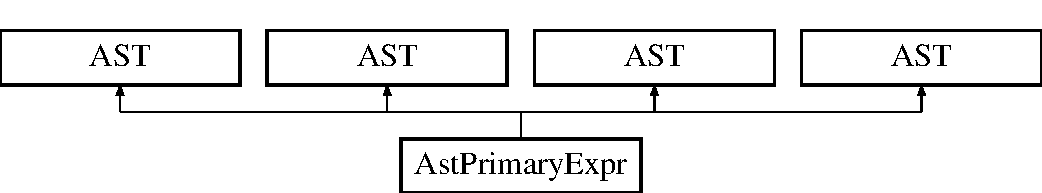
\includegraphics[height=2.000000cm]{classAstPrimaryExpr}
\end{center}
\end{figure}
\subsection*{Public Member Functions}
\begin{DoxyCompactItemize}
\item 
\hypertarget{classAstPrimaryExpr_a92ac6a98d42e522c7476768c959e2044}{{\bfseries Ast\-Primary\-Expr} (\hyperlink{classAstID}{Ast\-I\-D} $\ast$id)}\label{classAstPrimaryExpr_a92ac6a98d42e522c7476768c959e2044}

\item 
\hypertarget{classAstPrimaryExpr_a03809c945a11ab5345f50956cff84f82}{{\bfseries Ast\-Primary\-Expr} (\hyperlink{classAstConstant}{Ast\-Constant} $\ast$c)}\label{classAstPrimaryExpr_a03809c945a11ab5345f50956cff84f82}

\item 
\hypertarget{classAstPrimaryExpr_a784c92261d262fe4952963af0dd891e7}{{\bfseries Ast\-Primary\-Expr} (\hyperlink{classAstString}{Ast\-String} $\ast$s)}\label{classAstPrimaryExpr_a784c92261d262fe4952963af0dd891e7}

\item 
\hypertarget{classAstPrimaryExpr_a75b1363ac6a376ea3de63e03700072d8}{{\bfseries Ast\-Primary\-Expr} (\hyperlink{classAstExpression}{Ast\-Expression} $\ast$e)}\label{classAstPrimaryExpr_a75b1363ac6a376ea3de63e03700072d8}

\item 
\hypertarget{classAstPrimaryExpr_a0c5a0ec5399baf9dd319ba0f77e9111e}{\hyperlink{classAstID}{Ast\-I\-D} $\ast$ {\bfseries Get\-I\-D} ()}\label{classAstPrimaryExpr_a0c5a0ec5399baf9dd319ba0f77e9111e}

\item 
void \hyperlink{classAstPrimaryExpr_adfc316933183cada2963b7b855ddb824}{Visit} ()
\begin{DoxyCompactList}\small\item\em This function is responsible for tree traversals. \end{DoxyCompactList}\item 
\hypertarget{classAstPrimaryExpr_a92ac6a98d42e522c7476768c959e2044}{{\bfseries Ast\-Primary\-Expr} (\hyperlink{classAstID}{Ast\-I\-D} $\ast$id)}\label{classAstPrimaryExpr_a92ac6a98d42e522c7476768c959e2044}

\item 
\hypertarget{classAstPrimaryExpr_a03809c945a11ab5345f50956cff84f82}{{\bfseries Ast\-Primary\-Expr} (\hyperlink{classAstConstant}{Ast\-Constant} $\ast$c)}\label{classAstPrimaryExpr_a03809c945a11ab5345f50956cff84f82}

\item 
\hypertarget{classAstPrimaryExpr_a784c92261d262fe4952963af0dd891e7}{{\bfseries Ast\-Primary\-Expr} (\hyperlink{classAstString}{Ast\-String} $\ast$s)}\label{classAstPrimaryExpr_a784c92261d262fe4952963af0dd891e7}

\item 
\hypertarget{classAstPrimaryExpr_a75b1363ac6a376ea3de63e03700072d8}{{\bfseries Ast\-Primary\-Expr} (\hyperlink{classAstExpression}{Ast\-Expression} $\ast$e)}\label{classAstPrimaryExpr_a75b1363ac6a376ea3de63e03700072d8}

\item 
\hypertarget{classAstPrimaryExpr_a0c5a0ec5399baf9dd319ba0f77e9111e}{\hyperlink{classAstID}{Ast\-I\-D} $\ast$ {\bfseries Get\-I\-D} ()}\label{classAstPrimaryExpr_a0c5a0ec5399baf9dd319ba0f77e9111e}

\item 
void \hyperlink{classAstPrimaryExpr_adfc316933183cada2963b7b855ddb824}{Visit} ()
\begin{DoxyCompactList}\small\item\em This function is responsible for tree traversals. \end{DoxyCompactList}\item 
\hypertarget{classAstPrimaryExpr_a92ac6a98d42e522c7476768c959e2044}{{\bfseries Ast\-Primary\-Expr} (\hyperlink{classAstID}{Ast\-I\-D} $\ast$id)}\label{classAstPrimaryExpr_a92ac6a98d42e522c7476768c959e2044}

\item 
\hypertarget{classAstPrimaryExpr_a03809c945a11ab5345f50956cff84f82}{{\bfseries Ast\-Primary\-Expr} (\hyperlink{classAstConstant}{Ast\-Constant} $\ast$c)}\label{classAstPrimaryExpr_a03809c945a11ab5345f50956cff84f82}

\item 
\hypertarget{classAstPrimaryExpr_a784c92261d262fe4952963af0dd891e7}{{\bfseries Ast\-Primary\-Expr} (\hyperlink{classAstString}{Ast\-String} $\ast$s)}\label{classAstPrimaryExpr_a784c92261d262fe4952963af0dd891e7}

\item 
\hypertarget{classAstPrimaryExpr_a75b1363ac6a376ea3de63e03700072d8}{{\bfseries Ast\-Primary\-Expr} (\hyperlink{classAstExpression}{Ast\-Expression} $\ast$e)}\label{classAstPrimaryExpr_a75b1363ac6a376ea3de63e03700072d8}

\item 
\hypertarget{classAstPrimaryExpr_a0c5a0ec5399baf9dd319ba0f77e9111e}{\hyperlink{classAstID}{Ast\-I\-D} $\ast$ {\bfseries Get\-I\-D} ()}\label{classAstPrimaryExpr_a0c5a0ec5399baf9dd319ba0f77e9111e}

\item 
void \hyperlink{classAstPrimaryExpr_adfc316933183cada2963b7b855ddb824}{Visit} ()
\begin{DoxyCompactList}\small\item\em This function is responsible for tree traversals. \end{DoxyCompactList}\item 
\hypertarget{classAstPrimaryExpr_a92ac6a98d42e522c7476768c959e2044}{{\bfseries Ast\-Primary\-Expr} (\hyperlink{classAstID}{Ast\-I\-D} $\ast$id)}\label{classAstPrimaryExpr_a92ac6a98d42e522c7476768c959e2044}

\item 
\hypertarget{classAstPrimaryExpr_a03809c945a11ab5345f50956cff84f82}{{\bfseries Ast\-Primary\-Expr} (\hyperlink{classAstConstant}{Ast\-Constant} $\ast$c)}\label{classAstPrimaryExpr_a03809c945a11ab5345f50956cff84f82}

\item 
\hypertarget{classAstPrimaryExpr_a784c92261d262fe4952963af0dd891e7}{{\bfseries Ast\-Primary\-Expr} (\hyperlink{classAstString}{Ast\-String} $\ast$s)}\label{classAstPrimaryExpr_a784c92261d262fe4952963af0dd891e7}

\item 
\hypertarget{classAstPrimaryExpr_a75b1363ac6a376ea3de63e03700072d8}{{\bfseries Ast\-Primary\-Expr} (\hyperlink{classAstExpression}{Ast\-Expression} $\ast$e)}\label{classAstPrimaryExpr_a75b1363ac6a376ea3de63e03700072d8}

\item 
\hypertarget{classAstPrimaryExpr_a0c5a0ec5399baf9dd319ba0f77e9111e}{\hyperlink{classAstID}{Ast\-I\-D} $\ast$ {\bfseries Get\-I\-D} ()}\label{classAstPrimaryExpr_a0c5a0ec5399baf9dd319ba0f77e9111e}

\item 
void \hyperlink{classAstPrimaryExpr_adfc316933183cada2963b7b855ddb824}{Visit} ()
\begin{DoxyCompactList}\small\item\em This function is responsible for tree traversals. \end{DoxyCompactList}\item 
void \hyperlink{classAST_a71d680856e95ff89f55d5311a552eba6}{set\-Label} (string l)
\begin{DoxyCompactList}\small\item\em Sets the label for the node. \end{DoxyCompactList}\item 
void \hyperlink{classAST_a71d680856e95ff89f55d5311a552eba6}{set\-Label} (string l)
\begin{DoxyCompactList}\small\item\em Sets the label for the node. \end{DoxyCompactList}\item 
void \hyperlink{classAST_a71d680856e95ff89f55d5311a552eba6}{set\-Label} (string l)
\begin{DoxyCompactList}\small\item\em Sets the label for the node. \end{DoxyCompactList}\item 
void \hyperlink{classAST_a71d680856e95ff89f55d5311a552eba6}{set\-Label} (string l)
\begin{DoxyCompactList}\small\item\em Sets the label for the node. \end{DoxyCompactList}\item 
int \hyperlink{classAST_ab7a5b1d9f1c2de0d98deb356f724a42c}{get\-U\-I\-D} ()
\begin{DoxyCompactList}\small\item\em Gets the node's unique I\-D. \end{DoxyCompactList}\item 
int \hyperlink{classAST_ab7a5b1d9f1c2de0d98deb356f724a42c}{get\-U\-I\-D} ()
\begin{DoxyCompactList}\small\item\em Gets the node's unique I\-D. \end{DoxyCompactList}\item 
int \hyperlink{classAST_ab7a5b1d9f1c2de0d98deb356f724a42c}{get\-U\-I\-D} ()
\begin{DoxyCompactList}\small\item\em Gets the node's unique I\-D. \end{DoxyCompactList}\item 
int \hyperlink{classAST_ab7a5b1d9f1c2de0d98deb356f724a42c}{get\-U\-I\-D} ()
\begin{DoxyCompactList}\small\item\em Gets the node's unique I\-D. \end{DoxyCompactList}\item 
string \hyperlink{classAST_aee029be902fffc927d16ccb03eb922ad}{get\-Label} ()
\begin{DoxyCompactList}\small\item\em Gets the node's label. \end{DoxyCompactList}\item 
string \hyperlink{classAST_aee029be902fffc927d16ccb03eb922ad}{get\-Label} ()
\begin{DoxyCompactList}\small\item\em Gets the node's label. \end{DoxyCompactList}\item 
string \hyperlink{classAST_aee029be902fffc927d16ccb03eb922ad}{get\-Label} ()
\begin{DoxyCompactList}\small\item\em Gets the node's label. \end{DoxyCompactList}\item 
string \hyperlink{classAST_aee029be902fffc927d16ccb03eb922ad}{get\-Label} ()
\begin{DoxyCompactList}\small\item\em Gets the node's label. \end{DoxyCompactList}\end{DoxyCompactItemize}
\subsection*{Public Attributes}
\begin{DoxyCompactItemize}
\item 
\hypertarget{classAstPrimaryExpr_a872f9d089ce72fa3679bca3b40e1ba77}{\hyperlink{classType}{Type} $\ast$ {\bfseries etype}}\label{classAstPrimaryExpr_a872f9d089ce72fa3679bca3b40e1ba77}

\item 
\hypertarget{classAST_aaf215802de409f8096c063d01ffa6783}{bool \hyperlink{classAST_aaf215802de409f8096c063d01ffa6783}{needs\-Cast}}\label{classAST_aaf215802de409f8096c063d01ffa6783}

\begin{DoxyCompactList}\small\item\em This indicates if cast 3\-A\-C needs to be output, and is only relevant for expressions. \end{DoxyCompactList}\item 
\hypertarget{classAST_afa9e77ef650ec6664458fa6cb55be985}{bool \hyperlink{classAST_afa9e77ef650ec6664458fa6cb55be985}{is\-Conv}}\label{classAST_afa9e77ef650ec6664458fa6cb55be985}

\begin{DoxyCompactList}\small\item\em Indicates is a conversion is possible. \end{DoxyCompactList}\item 
\hypertarget{classAST_a61ef3317e023d45237e06615b387cd6b}{C\-O\-N\-V\-E\-R\-S\-I\-O\-N\-T\-Y\-P\-E \hyperlink{classAST_a61ef3317e023d45237e06615b387cd6b}{conv\-Type}}\label{classAST_a61ef3317e023d45237e06615b387cd6b}

\begin{DoxyCompactList}\small\item\em If needs\-Cast is true, then this indicates what the cast should be. \end{DoxyCompactList}\item 
\hypertarget{classAST_aea9b07b39d24183f38c0029cec0a878e}{int \hyperlink{classAST_aea9b07b39d24183f38c0029cec0a878e}{operand\-To\-Cast}}\label{classAST_aea9b07b39d24183f38c0029cec0a878e}

\begin{DoxyCompactList}\small\item\em This indicates if the first or second operand should be the one that is cast. \end{DoxyCompactList}\end{DoxyCompactItemize}
\subsection*{Static Public Attributes}
\begin{DoxyCompactItemize}
\item 
\hypertarget{classAST_a5fdfd5f7b104dd92889163bdadbc68d6}{static \hyperlink{classVisualizer}{Visualizer} \hyperlink{classAST_a5fdfd5f7b104dd92889163bdadbc68d6}{vis}}\label{classAST_a5fdfd5f7b104dd92889163bdadbc68d6}

\begin{DoxyCompactList}\small\item\em Static visualizer instance for generating the visualization of the \hyperlink{classAST}{A\-S\-T}. \end{DoxyCompactList}\item 
\hypertarget{classAST_a8a3ace322f50e030331065d644ee55ee}{static \hyperlink{classTAC__Generator}{T\-A\-C\-\_\-\-Generator} \hyperlink{classAST_a8a3ace322f50e030331065d644ee55ee}{tac\-Gen}}\label{classAST_a8a3ace322f50e030331065d644ee55ee}

\begin{DoxyCompactList}\small\item\em Three address code generator. \end{DoxyCompactList}\item 
\hypertarget{classAST_a1f69448c6dc368d005631a128460083d}{static string {\bfseries current\-Temp} =\char`\"{}\char`\"{}}\label{classAST_a1f69448c6dc368d005631a128460083d}

\item 
\hypertarget{classAST_a551aec090c932ab69365238b40a8a4eb}{static string \hyperlink{classAST_a551aec090c932ab69365238b40a8a4eb}{return\-Label} =\char`\"{}\char`\"{}}\label{classAST_a551aec090c932ab69365238b40a8a4eb}

\begin{DoxyCompactList}\small\item\em This is for storing the string id of any temporary result register that may be created during 3\-A\-C generation. \end{DoxyCompactList}\item 
\hypertarget{classAST_a73c0a266df52be71e6b527b6aa635173}{static list$<$ string $>$ {\bfseries temp\-Stack}}\label{classAST_a73c0a266df52be71e6b527b6aa635173}

\item 
\hypertarget{classAST_abf9e84b541ff04b7bb64e6e4371512d4}{static string {\bfseries last\-I\-D} =\char`\"{}\char`\"{}}\label{classAST_abf9e84b541ff04b7bb64e6e4371512d4}

\item 
\hypertarget{classAST_a163003bfe9c30510ec8039870346049f}{static \hyperlink{classSymTab}{Sym\-Tab} $\ast$ {\bfseries symbol\-Table} =N\-U\-L\-L}\label{classAST_a163003bfe9c30510ec8039870346049f}

\item 
\hypertarget{classAST_a5c3cc894d9c0453523dec9ed76f18a04}{static string {\bfseries current\-Function} =\char`\"{}\char`\"{}}\label{classAST_a5c3cc894d9c0453523dec9ed76f18a04}

\item 
\hypertarget{classAST_a66155513b59ff1a04c8ece8b20ec31f5}{static int {\bfseries current\-Constant\-Value} =0}\label{classAST_a66155513b59ff1a04c8ece8b20ec31f5}

\item 
\hypertarget{classAST_a3d031d7bab635ba1f015aade5943f40c}{static string {\bfseries current\-Id\-Name} =\char`\"{}\char`\"{}}\label{classAST_a3d031d7bab635ba1f015aade5943f40c}

\item 
\hypertarget{classAST_a16c4b6e54febc1a26b31a64a46972ef0}{static int {\bfseries current\-Index\-Val} = 0}\label{classAST_a16c4b6e54febc1a26b31a64a46972ef0}

\item 
\hypertarget{classAST_a6fc65ae9dd064a88941d4b88669b19db}{static string {\bfseries current\-I\-D} = \char`\"{}\char`\"{}}\label{classAST_a6fc65ae9dd064a88941d4b88669b19db}

\end{DoxyCompactItemize}
\subsection*{Protected Attributes}
\begin{DoxyCompactItemize}
\item 
\hypertarget{classAST_a847b778f1c3dd5a19de32de432ee6e15}{int \hyperlink{classAST_a847b778f1c3dd5a19de32de432ee6e15}{uid}}\label{classAST_a847b778f1c3dd5a19de32de432ee6e15}

\begin{DoxyCompactList}\small\item\em The unique id. \end{DoxyCompactList}\item 
\hypertarget{classAST_ab2e239ccc0688d2341724432ff5a1a31}{string \hyperlink{classAST_ab2e239ccc0688d2341724432ff5a1a31}{label}}\label{classAST_ab2e239ccc0688d2341724432ff5a1a31}

\begin{DoxyCompactList}\small\item\em The label to be printed in the visualization. \end{DoxyCompactList}\end{DoxyCompactItemize}
\subsection*{Private Types}
\begin{DoxyCompactItemize}
\item 
enum {\bfseries Expr\-Type} \{ \\*
{\bfseries I\-D}, 
{\bfseries C\-O\-N\-S\-T}, 
{\bfseries S\-T\-R\-I\-N\-G}, 
{\bfseries E\-X\-P\-R}, 
\\*
{\bfseries I\-D}, 
{\bfseries C\-O\-N\-S\-T}, 
{\bfseries S\-T\-R\-I\-N\-G}, 
{\bfseries E\-X\-P\-R}, 
\\*
{\bfseries I\-D}, 
{\bfseries C\-O\-N\-S\-T}, 
{\bfseries S\-T\-R\-I\-N\-G}, 
{\bfseries E\-X\-P\-R}, 
\\*
{\bfseries I\-D}, 
{\bfseries C\-O\-N\-S\-T}, 
{\bfseries S\-T\-R\-I\-N\-G}, 
{\bfseries E\-X\-P\-R}
 \}
\item 
enum {\bfseries Expr\-Type} \{ \\*
{\bfseries I\-D}, 
{\bfseries C\-O\-N\-S\-T}, 
{\bfseries S\-T\-R\-I\-N\-G}, 
{\bfseries E\-X\-P\-R}, 
\\*
{\bfseries I\-D}, 
{\bfseries C\-O\-N\-S\-T}, 
{\bfseries S\-T\-R\-I\-N\-G}, 
{\bfseries E\-X\-P\-R}, 
\\*
{\bfseries I\-D}, 
{\bfseries C\-O\-N\-S\-T}, 
{\bfseries S\-T\-R\-I\-N\-G}, 
{\bfseries E\-X\-P\-R}, 
\\*
{\bfseries I\-D}, 
{\bfseries C\-O\-N\-S\-T}, 
{\bfseries S\-T\-R\-I\-N\-G}, 
{\bfseries E\-X\-P\-R}
 \}
\item 
enum {\bfseries Expr\-Type} \{ \\*
{\bfseries I\-D}, 
{\bfseries C\-O\-N\-S\-T}, 
{\bfseries S\-T\-R\-I\-N\-G}, 
{\bfseries E\-X\-P\-R}, 
\\*
{\bfseries I\-D}, 
{\bfseries C\-O\-N\-S\-T}, 
{\bfseries S\-T\-R\-I\-N\-G}, 
{\bfseries E\-X\-P\-R}, 
\\*
{\bfseries I\-D}, 
{\bfseries C\-O\-N\-S\-T}, 
{\bfseries S\-T\-R\-I\-N\-G}, 
{\bfseries E\-X\-P\-R}, 
\\*
{\bfseries I\-D}, 
{\bfseries C\-O\-N\-S\-T}, 
{\bfseries S\-T\-R\-I\-N\-G}, 
{\bfseries E\-X\-P\-R}
 \}
\item 
enum {\bfseries Expr\-Type} \{ \\*
{\bfseries I\-D}, 
{\bfseries C\-O\-N\-S\-T}, 
{\bfseries S\-T\-R\-I\-N\-G}, 
{\bfseries E\-X\-P\-R}, 
\\*
{\bfseries I\-D}, 
{\bfseries C\-O\-N\-S\-T}, 
{\bfseries S\-T\-R\-I\-N\-G}, 
{\bfseries E\-X\-P\-R}, 
\\*
{\bfseries I\-D}, 
{\bfseries C\-O\-N\-S\-T}, 
{\bfseries S\-T\-R\-I\-N\-G}, 
{\bfseries E\-X\-P\-R}, 
\\*
{\bfseries I\-D}, 
{\bfseries C\-O\-N\-S\-T}, 
{\bfseries S\-T\-R\-I\-N\-G}, 
{\bfseries E\-X\-P\-R}
 \}
\end{DoxyCompactItemize}
\subsection*{Private Attributes}
\begin{DoxyCompactItemize}
\item 
\hypertarget{classAstPrimaryExpr_a591ec0d1a62cf2017702676cc3e71f72}{Expr\-Type {\bfseries type}}\label{classAstPrimaryExpr_a591ec0d1a62cf2017702676cc3e71f72}

\item 
\hypertarget{classAstPrimaryExpr_a68d2d82410c66710af8ed7ef339ce6ae}{\hyperlink{classAstID}{Ast\-I\-D} $\ast$ {\bfseries id}}\label{classAstPrimaryExpr_a68d2d82410c66710af8ed7ef339ce6ae}

\item 
\hypertarget{classAstPrimaryExpr_aab1c10499b5ac67eb25b075d8ed91651}{\hyperlink{classAstConstant}{Ast\-Constant} $\ast$ {\bfseries constant}}\label{classAstPrimaryExpr_aab1c10499b5ac67eb25b075d8ed91651}

\item 
\hypertarget{classAstPrimaryExpr_acd34a00f1d811cdf233302266befead4}{\hyperlink{classAstString}{Ast\-String} $\ast$ {\bfseries str}}\label{classAstPrimaryExpr_acd34a00f1d811cdf233302266befead4}

\item 
\hypertarget{classAstPrimaryExpr_a7a1f4a43c1dff07fc59e5c774b8f4f58}{\hyperlink{classAstExpression}{Ast\-Expression} $\ast$ {\bfseries expr}}\label{classAstPrimaryExpr_a7a1f4a43c1dff07fc59e5c774b8f4f58}

\end{DoxyCompactItemize}


\subsection{Detailed Description}


Definition at line 248 of file Ast.\-h.



\subsection{Member Function Documentation}
\hypertarget{classAST_aee029be902fffc927d16ccb03eb922ad}{\index{Ast\-Primary\-Expr@{Ast\-Primary\-Expr}!get\-Label@{get\-Label}}
\index{get\-Label@{get\-Label}!AstPrimaryExpr@{Ast\-Primary\-Expr}}
\subsubsection[{get\-Label}]{\setlength{\rightskip}{0pt plus 5cm}string A\-S\-T\-::get\-Label (
\begin{DoxyParamCaption}
{}
\end{DoxyParamCaption}
)\hspace{0.3cm}{\ttfamily [inline]}, {\ttfamily [inherited]}}}\label{classAST_aee029be902fffc927d16ccb03eb922ad}


Gets the node's label. 

\begin{DoxyReturn}{Returns}
The label 
\end{DoxyReturn}


Definition at line 60 of file Ast.\-h.

\hypertarget{classAST_aee029be902fffc927d16ccb03eb922ad}{\index{Ast\-Primary\-Expr@{Ast\-Primary\-Expr}!get\-Label@{get\-Label}}
\index{get\-Label@{get\-Label}!AstPrimaryExpr@{Ast\-Primary\-Expr}}
\subsubsection[{get\-Label}]{\setlength{\rightskip}{0pt plus 5cm}string A\-S\-T\-::get\-Label (
\begin{DoxyParamCaption}
{}
\end{DoxyParamCaption}
)\hspace{0.3cm}{\ttfamily [inline]}, {\ttfamily [inherited]}}}\label{classAST_aee029be902fffc927d16ccb03eb922ad}


Gets the node's label. 

\begin{DoxyReturn}{Returns}
The label 
\end{DoxyReturn}


Definition at line 60 of file C\-Parser.\-yy.

\hypertarget{classAST_aee029be902fffc927d16ccb03eb922ad}{\index{Ast\-Primary\-Expr@{Ast\-Primary\-Expr}!get\-Label@{get\-Label}}
\index{get\-Label@{get\-Label}!AstPrimaryExpr@{Ast\-Primary\-Expr}}
\subsubsection[{get\-Label}]{\setlength{\rightskip}{0pt plus 5cm}string A\-S\-T\-::get\-Label (
\begin{DoxyParamCaption}
{}
\end{DoxyParamCaption}
)\hspace{0.3cm}{\ttfamily [inline]}, {\ttfamily [inherited]}}}\label{classAST_aee029be902fffc927d16ccb03eb922ad}


Gets the node's label. 

\begin{DoxyReturn}{Returns}
The label 
\end{DoxyReturn}


Definition at line 60 of file C\-Parser.\-yy.

\hypertarget{classAST_aee029be902fffc927d16ccb03eb922ad}{\index{Ast\-Primary\-Expr@{Ast\-Primary\-Expr}!get\-Label@{get\-Label}}
\index{get\-Label@{get\-Label}!AstPrimaryExpr@{Ast\-Primary\-Expr}}
\subsubsection[{get\-Label}]{\setlength{\rightskip}{0pt plus 5cm}string A\-S\-T\-::get\-Label (
\begin{DoxyParamCaption}
{}
\end{DoxyParamCaption}
)\hspace{0.3cm}{\ttfamily [inline]}, {\ttfamily [inherited]}}}\label{classAST_aee029be902fffc927d16ccb03eb922ad}


Gets the node's label. 

\begin{DoxyReturn}{Returns}
The label 
\end{DoxyReturn}


Definition at line 60 of file C\-Scanner.\-ll.

\hypertarget{classAST_ab7a5b1d9f1c2de0d98deb356f724a42c}{\index{Ast\-Primary\-Expr@{Ast\-Primary\-Expr}!get\-U\-I\-D@{get\-U\-I\-D}}
\index{get\-U\-I\-D@{get\-U\-I\-D}!AstPrimaryExpr@{Ast\-Primary\-Expr}}
\subsubsection[{get\-U\-I\-D}]{\setlength{\rightskip}{0pt plus 5cm}int A\-S\-T\-::get\-U\-I\-D (
\begin{DoxyParamCaption}
{}
\end{DoxyParamCaption}
)\hspace{0.3cm}{\ttfamily [inline]}, {\ttfamily [inherited]}}}\label{classAST_ab7a5b1d9f1c2de0d98deb356f724a42c}


Gets the node's unique I\-D. 

\begin{DoxyReturn}{Returns}
The unique id 
\end{DoxyReturn}


Definition at line 53 of file C\-Scanner.\-ll.

\hypertarget{classAST_ab7a5b1d9f1c2de0d98deb356f724a42c}{\index{Ast\-Primary\-Expr@{Ast\-Primary\-Expr}!get\-U\-I\-D@{get\-U\-I\-D}}
\index{get\-U\-I\-D@{get\-U\-I\-D}!AstPrimaryExpr@{Ast\-Primary\-Expr}}
\subsubsection[{get\-U\-I\-D}]{\setlength{\rightskip}{0pt plus 5cm}int A\-S\-T\-::get\-U\-I\-D (
\begin{DoxyParamCaption}
{}
\end{DoxyParamCaption}
)\hspace{0.3cm}{\ttfamily [inline]}, {\ttfamily [inherited]}}}\label{classAST_ab7a5b1d9f1c2de0d98deb356f724a42c}


Gets the node's unique I\-D. 

\begin{DoxyReturn}{Returns}
The unique id 
\end{DoxyReturn}


Definition at line 53 of file C\-Parser.\-yy.

\hypertarget{classAST_ab7a5b1d9f1c2de0d98deb356f724a42c}{\index{Ast\-Primary\-Expr@{Ast\-Primary\-Expr}!get\-U\-I\-D@{get\-U\-I\-D}}
\index{get\-U\-I\-D@{get\-U\-I\-D}!AstPrimaryExpr@{Ast\-Primary\-Expr}}
\subsubsection[{get\-U\-I\-D}]{\setlength{\rightskip}{0pt plus 5cm}int A\-S\-T\-::get\-U\-I\-D (
\begin{DoxyParamCaption}
{}
\end{DoxyParamCaption}
)\hspace{0.3cm}{\ttfamily [inline]}, {\ttfamily [inherited]}}}\label{classAST_ab7a5b1d9f1c2de0d98deb356f724a42c}


Gets the node's unique I\-D. 

\begin{DoxyReturn}{Returns}
The unique id 
\end{DoxyReturn}


Definition at line 53 of file Ast.\-h.

\hypertarget{classAST_ab7a5b1d9f1c2de0d98deb356f724a42c}{\index{Ast\-Primary\-Expr@{Ast\-Primary\-Expr}!get\-U\-I\-D@{get\-U\-I\-D}}
\index{get\-U\-I\-D@{get\-U\-I\-D}!AstPrimaryExpr@{Ast\-Primary\-Expr}}
\subsubsection[{get\-U\-I\-D}]{\setlength{\rightskip}{0pt plus 5cm}int A\-S\-T\-::get\-U\-I\-D (
\begin{DoxyParamCaption}
{}
\end{DoxyParamCaption}
)\hspace{0.3cm}{\ttfamily [inline]}, {\ttfamily [inherited]}}}\label{classAST_ab7a5b1d9f1c2de0d98deb356f724a42c}


Gets the node's unique I\-D. 

\begin{DoxyReturn}{Returns}
The unique id 
\end{DoxyReturn}


Definition at line 53 of file C\-Parser.\-yy.

\hypertarget{classAST_a71d680856e95ff89f55d5311a552eba6}{\index{Ast\-Primary\-Expr@{Ast\-Primary\-Expr}!set\-Label@{set\-Label}}
\index{set\-Label@{set\-Label}!AstPrimaryExpr@{Ast\-Primary\-Expr}}
\subsubsection[{set\-Label}]{\setlength{\rightskip}{0pt plus 5cm}void A\-S\-T\-::set\-Label (
\begin{DoxyParamCaption}
\item[{string}]{l}
\end{DoxyParamCaption}
)\hspace{0.3cm}{\ttfamily [inline]}, {\ttfamily [inherited]}}}\label{classAST_a71d680856e95ff89f55d5311a552eba6}


Sets the label for the node. 


\begin{DoxyParams}{Parameters}
{\em l} & The label string \\
\hline
\end{DoxyParams}


Definition at line 43 of file Ast.\-h.

\hypertarget{classAST_a71d680856e95ff89f55d5311a552eba6}{\index{Ast\-Primary\-Expr@{Ast\-Primary\-Expr}!set\-Label@{set\-Label}}
\index{set\-Label@{set\-Label}!AstPrimaryExpr@{Ast\-Primary\-Expr}}
\subsubsection[{set\-Label}]{\setlength{\rightskip}{0pt plus 5cm}void A\-S\-T\-::set\-Label (
\begin{DoxyParamCaption}
\item[{string}]{l}
\end{DoxyParamCaption}
)\hspace{0.3cm}{\ttfamily [inline]}, {\ttfamily [inherited]}}}\label{classAST_a71d680856e95ff89f55d5311a552eba6}


Sets the label for the node. 


\begin{DoxyParams}{Parameters}
{\em l} & The label string \\
\hline
\end{DoxyParams}


Definition at line 43 of file C\-Parser.\-yy.

\hypertarget{classAST_a71d680856e95ff89f55d5311a552eba6}{\index{Ast\-Primary\-Expr@{Ast\-Primary\-Expr}!set\-Label@{set\-Label}}
\index{set\-Label@{set\-Label}!AstPrimaryExpr@{Ast\-Primary\-Expr}}
\subsubsection[{set\-Label}]{\setlength{\rightskip}{0pt plus 5cm}void A\-S\-T\-::set\-Label (
\begin{DoxyParamCaption}
\item[{string}]{l}
\end{DoxyParamCaption}
)\hspace{0.3cm}{\ttfamily [inline]}, {\ttfamily [inherited]}}}\label{classAST_a71d680856e95ff89f55d5311a552eba6}


Sets the label for the node. 


\begin{DoxyParams}{Parameters}
{\em l} & The label string \\
\hline
\end{DoxyParams}


Definition at line 43 of file C\-Parser.\-yy.

\hypertarget{classAST_a71d680856e95ff89f55d5311a552eba6}{\index{Ast\-Primary\-Expr@{Ast\-Primary\-Expr}!set\-Label@{set\-Label}}
\index{set\-Label@{set\-Label}!AstPrimaryExpr@{Ast\-Primary\-Expr}}
\subsubsection[{set\-Label}]{\setlength{\rightskip}{0pt plus 5cm}void A\-S\-T\-::set\-Label (
\begin{DoxyParamCaption}
\item[{string}]{l}
\end{DoxyParamCaption}
)\hspace{0.3cm}{\ttfamily [inline]}, {\ttfamily [inherited]}}}\label{classAST_a71d680856e95ff89f55d5311a552eba6}


Sets the label for the node. 


\begin{DoxyParams}{Parameters}
{\em l} & The label string \\
\hline
\end{DoxyParams}


Definition at line 43 of file C\-Scanner.\-ll.

\hypertarget{classAstPrimaryExpr_adfc316933183cada2963b7b855ddb824}{\index{Ast\-Primary\-Expr@{Ast\-Primary\-Expr}!Visit@{Visit}}
\index{Visit@{Visit}!AstPrimaryExpr@{Ast\-Primary\-Expr}}
\subsubsection[{Visit}]{\setlength{\rightskip}{0pt plus 5cm}void Ast\-Primary\-Expr\-::\-Visit (
\begin{DoxyParamCaption}
{}
\end{DoxyParamCaption}
)\hspace{0.3cm}{\ttfamily [virtual]}}}\label{classAstPrimaryExpr_adfc316933183cada2963b7b855ddb824}


This function is responsible for tree traversals. 

This function will call the Visit functions of each of it's children nodes, call the visualization code for itself, and output any 3\-A\-C that can be generated at the current node. 

Reimplemented from \hyperlink{classAST_a5828cc86f2c4f1a0aeab6d7069e8fd82}{A\-S\-T}.



Definition at line 71 of file Ast.\-cpp.

\hypertarget{classAstPrimaryExpr_adfc316933183cada2963b7b855ddb824}{\index{Ast\-Primary\-Expr@{Ast\-Primary\-Expr}!Visit@{Visit}}
\index{Visit@{Visit}!AstPrimaryExpr@{Ast\-Primary\-Expr}}
\subsubsection[{Visit}]{\setlength{\rightskip}{0pt plus 5cm}void Ast\-Primary\-Expr\-::\-Visit (
\begin{DoxyParamCaption}
{}
\end{DoxyParamCaption}
)\hspace{0.3cm}{\ttfamily [virtual]}}}\label{classAstPrimaryExpr_adfc316933183cada2963b7b855ddb824}


This function is responsible for tree traversals. 

This function will call the Visit functions of each of it's children nodes, call the visualization code for itself, and output any 3\-A\-C that can be generated at the current node. 

Reimplemented from \hyperlink{classAST_a5828cc86f2c4f1a0aeab6d7069e8fd82}{A\-S\-T}.

\hypertarget{classAstPrimaryExpr_adfc316933183cada2963b7b855ddb824}{\index{Ast\-Primary\-Expr@{Ast\-Primary\-Expr}!Visit@{Visit}}
\index{Visit@{Visit}!AstPrimaryExpr@{Ast\-Primary\-Expr}}
\subsubsection[{Visit}]{\setlength{\rightskip}{0pt plus 5cm}void Ast\-Primary\-Expr\-::\-Visit (
\begin{DoxyParamCaption}
{}
\end{DoxyParamCaption}
)\hspace{0.3cm}{\ttfamily [virtual]}}}\label{classAstPrimaryExpr_adfc316933183cada2963b7b855ddb824}


This function is responsible for tree traversals. 

This function will call the Visit functions of each of it's children nodes, call the visualization code for itself, and output any 3\-A\-C that can be generated at the current node. 

Reimplemented from \hyperlink{classAST_a5828cc86f2c4f1a0aeab6d7069e8fd82}{A\-S\-T}.

\hypertarget{classAstPrimaryExpr_adfc316933183cada2963b7b855ddb824}{\index{Ast\-Primary\-Expr@{Ast\-Primary\-Expr}!Visit@{Visit}}
\index{Visit@{Visit}!AstPrimaryExpr@{Ast\-Primary\-Expr}}
\subsubsection[{Visit}]{\setlength{\rightskip}{0pt plus 5cm}void Ast\-Primary\-Expr\-::\-Visit (
\begin{DoxyParamCaption}
{}
\end{DoxyParamCaption}
)\hspace{0.3cm}{\ttfamily [virtual]}}}\label{classAstPrimaryExpr_adfc316933183cada2963b7b855ddb824}


This function is responsible for tree traversals. 

This function will call the Visit functions of each of it's children nodes, call the visualization code for itself, and output any 3\-A\-C that can be generated at the current node. 

Reimplemented from \hyperlink{classAST_a5828cc86f2c4f1a0aeab6d7069e8fd82}{A\-S\-T}.



The documentation for this class was generated from the following files\-:\begin{DoxyCompactItemize}
\item 
Ast.\-h\item 
Ast.\-cpp\end{DoxyCompactItemize}

\hypertarget{classAstRelExpr}{\section{Ast\-Rel\-Expr Class Reference}
\label{classAstRelExpr}\index{Ast\-Rel\-Expr@{Ast\-Rel\-Expr}}
}
Inheritance diagram for Ast\-Rel\-Expr\-:\begin{figure}[H]
\begin{center}
\leavevmode
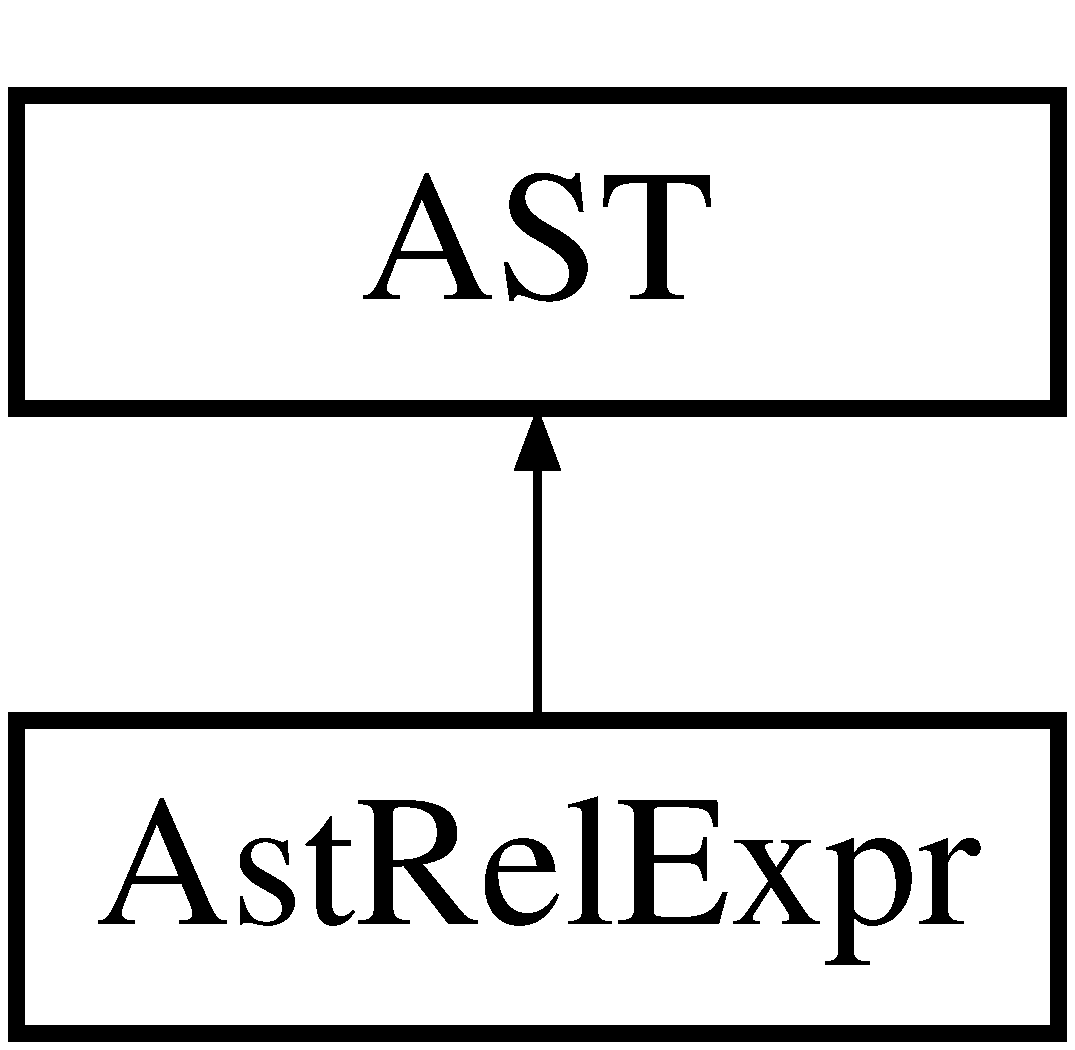
\includegraphics[height=2.000000cm]{classAstRelExpr}
\end{center}
\end{figure}
\subsection*{Public Types}
\begin{DoxyCompactItemize}
\item 
enum {\bfseries Operator} \{ \\*
{\bfseries N\-O\-N\-E}, 
{\bfseries L\-T\-\_\-\-O\-P}, 
{\bfseries G\-T\-\_\-\-O\-P}, 
{\bfseries L\-E\-\_\-\-O\-P}, 
\\*
{\bfseries G\-E\-\_\-\-O\-P}, 
{\bfseries N\-O\-N\-E}, 
{\bfseries L\-T\-\_\-\-O\-P}, 
{\bfseries G\-T\-\_\-\-O\-P}, 
\\*
{\bfseries L\-E\-\_\-\-O\-P}, 
{\bfseries G\-E\-\_\-\-O\-P}, 
{\bfseries N\-O\-N\-E}, 
{\bfseries L\-T\-\_\-\-O\-P}, 
\\*
{\bfseries G\-T\-\_\-\-O\-P}, 
{\bfseries L\-E\-\_\-\-O\-P}, 
{\bfseries G\-E\-\_\-\-O\-P}, 
{\bfseries N\-O\-N\-E}, 
\\*
{\bfseries L\-T\-\_\-\-O\-P}, 
{\bfseries G\-T\-\_\-\-O\-P}, 
{\bfseries L\-E\-\_\-\-O\-P}, 
{\bfseries G\-E\-\_\-\-O\-P}
 \}
\item 
enum {\bfseries Operator} \{ \\*
{\bfseries N\-O\-N\-E}, 
{\bfseries L\-T\-\_\-\-O\-P}, 
{\bfseries G\-T\-\_\-\-O\-P}, 
{\bfseries L\-E\-\_\-\-O\-P}, 
\\*
{\bfseries G\-E\-\_\-\-O\-P}, 
{\bfseries N\-O\-N\-E}, 
{\bfseries L\-T\-\_\-\-O\-P}, 
{\bfseries G\-T\-\_\-\-O\-P}, 
\\*
{\bfseries L\-E\-\_\-\-O\-P}, 
{\bfseries G\-E\-\_\-\-O\-P}, 
{\bfseries N\-O\-N\-E}, 
{\bfseries L\-T\-\_\-\-O\-P}, 
\\*
{\bfseries G\-T\-\_\-\-O\-P}, 
{\bfseries L\-E\-\_\-\-O\-P}, 
{\bfseries G\-E\-\_\-\-O\-P}, 
{\bfseries N\-O\-N\-E}, 
\\*
{\bfseries L\-T\-\_\-\-O\-P}, 
{\bfseries G\-T\-\_\-\-O\-P}, 
{\bfseries L\-E\-\_\-\-O\-P}, 
{\bfseries G\-E\-\_\-\-O\-P}
 \}
\item 
enum {\bfseries Operator} \{ \\*
{\bfseries N\-O\-N\-E}, 
{\bfseries L\-T\-\_\-\-O\-P}, 
{\bfseries G\-T\-\_\-\-O\-P}, 
{\bfseries L\-E\-\_\-\-O\-P}, 
\\*
{\bfseries G\-E\-\_\-\-O\-P}, 
{\bfseries N\-O\-N\-E}, 
{\bfseries L\-T\-\_\-\-O\-P}, 
{\bfseries G\-T\-\_\-\-O\-P}, 
\\*
{\bfseries L\-E\-\_\-\-O\-P}, 
{\bfseries G\-E\-\_\-\-O\-P}, 
{\bfseries N\-O\-N\-E}, 
{\bfseries L\-T\-\_\-\-O\-P}, 
\\*
{\bfseries G\-T\-\_\-\-O\-P}, 
{\bfseries L\-E\-\_\-\-O\-P}, 
{\bfseries G\-E\-\_\-\-O\-P}, 
{\bfseries N\-O\-N\-E}, 
\\*
{\bfseries L\-T\-\_\-\-O\-P}, 
{\bfseries G\-T\-\_\-\-O\-P}, 
{\bfseries L\-E\-\_\-\-O\-P}, 
{\bfseries G\-E\-\_\-\-O\-P}
 \}
\item 
enum {\bfseries Operator} \{ \\*
{\bfseries N\-O\-N\-E}, 
{\bfseries L\-T\-\_\-\-O\-P}, 
{\bfseries G\-T\-\_\-\-O\-P}, 
{\bfseries L\-E\-\_\-\-O\-P}, 
\\*
{\bfseries G\-E\-\_\-\-O\-P}, 
{\bfseries N\-O\-N\-E}, 
{\bfseries L\-T\-\_\-\-O\-P}, 
{\bfseries G\-T\-\_\-\-O\-P}, 
\\*
{\bfseries L\-E\-\_\-\-O\-P}, 
{\bfseries G\-E\-\_\-\-O\-P}, 
{\bfseries N\-O\-N\-E}, 
{\bfseries L\-T\-\_\-\-O\-P}, 
\\*
{\bfseries G\-T\-\_\-\-O\-P}, 
{\bfseries L\-E\-\_\-\-O\-P}, 
{\bfseries G\-E\-\_\-\-O\-P}, 
{\bfseries N\-O\-N\-E}, 
\\*
{\bfseries L\-T\-\_\-\-O\-P}, 
{\bfseries G\-T\-\_\-\-O\-P}, 
{\bfseries L\-E\-\_\-\-O\-P}, 
{\bfseries G\-E\-\_\-\-O\-P}
 \}
\end{DoxyCompactItemize}
\subsection*{Public Member Functions}
\begin{DoxyCompactItemize}
\item 
\hypertarget{classAstRelExpr_a17bddafe8d750f50ae41eb9c87410b1e}{{\bfseries Ast\-Rel\-Expr} (\hyperlink{classAstShiftExpr}{Ast\-Shift\-Expr} $\ast$s)}\label{classAstRelExpr_a17bddafe8d750f50ae41eb9c87410b1e}

\item 
\hypertarget{classAstRelExpr_a7a8c51e92d85456cd8da5b426f6958cf}{{\bfseries Ast\-Rel\-Expr} (\hyperlink{classAstRelExpr}{Ast\-Rel\-Expr} $\ast$r, Operator o, \hyperlink{classAstShiftExpr}{Ast\-Shift\-Expr} $\ast$s)}\label{classAstRelExpr_a7a8c51e92d85456cd8da5b426f6958cf}

\item 
void \hyperlink{classAstRelExpr_ae1a3ad7c0ce7a205222ec0b1de5ee884}{Visit} ()
\begin{DoxyCompactList}\small\item\em This function is responsible for tree traversals. \end{DoxyCompactList}\item 
\hypertarget{classAstRelExpr_a17bddafe8d750f50ae41eb9c87410b1e}{{\bfseries Ast\-Rel\-Expr} (\hyperlink{classAstShiftExpr}{Ast\-Shift\-Expr} $\ast$s)}\label{classAstRelExpr_a17bddafe8d750f50ae41eb9c87410b1e}

\item 
\hypertarget{classAstRelExpr_a7a8c51e92d85456cd8da5b426f6958cf}{{\bfseries Ast\-Rel\-Expr} (\hyperlink{classAstRelExpr}{Ast\-Rel\-Expr} $\ast$r, Operator o, \hyperlink{classAstShiftExpr}{Ast\-Shift\-Expr} $\ast$s)}\label{classAstRelExpr_a7a8c51e92d85456cd8da5b426f6958cf}

\item 
void \hyperlink{classAstRelExpr_ae1a3ad7c0ce7a205222ec0b1de5ee884}{Visit} ()
\begin{DoxyCompactList}\small\item\em This function is responsible for tree traversals. \end{DoxyCompactList}\item 
\hypertarget{classAstRelExpr_a17bddafe8d750f50ae41eb9c87410b1e}{{\bfseries Ast\-Rel\-Expr} (\hyperlink{classAstShiftExpr}{Ast\-Shift\-Expr} $\ast$s)}\label{classAstRelExpr_a17bddafe8d750f50ae41eb9c87410b1e}

\item 
\hypertarget{classAstRelExpr_a7a8c51e92d85456cd8da5b426f6958cf}{{\bfseries Ast\-Rel\-Expr} (\hyperlink{classAstRelExpr}{Ast\-Rel\-Expr} $\ast$r, Operator o, \hyperlink{classAstShiftExpr}{Ast\-Shift\-Expr} $\ast$s)}\label{classAstRelExpr_a7a8c51e92d85456cd8da5b426f6958cf}

\item 
void \hyperlink{classAstRelExpr_ae1a3ad7c0ce7a205222ec0b1de5ee884}{Visit} ()
\begin{DoxyCompactList}\small\item\em This function is responsible for tree traversals. \end{DoxyCompactList}\item 
\hypertarget{classAstRelExpr_a17bddafe8d750f50ae41eb9c87410b1e}{{\bfseries Ast\-Rel\-Expr} (\hyperlink{classAstShiftExpr}{Ast\-Shift\-Expr} $\ast$s)}\label{classAstRelExpr_a17bddafe8d750f50ae41eb9c87410b1e}

\item 
\hypertarget{classAstRelExpr_a7a8c51e92d85456cd8da5b426f6958cf}{{\bfseries Ast\-Rel\-Expr} (\hyperlink{classAstRelExpr}{Ast\-Rel\-Expr} $\ast$r, Operator o, \hyperlink{classAstShiftExpr}{Ast\-Shift\-Expr} $\ast$s)}\label{classAstRelExpr_a7a8c51e92d85456cd8da5b426f6958cf}

\item 
void \hyperlink{classAstRelExpr_ae1a3ad7c0ce7a205222ec0b1de5ee884}{Visit} ()
\begin{DoxyCompactList}\small\item\em This function is responsible for tree traversals. \end{DoxyCompactList}\item 
void \hyperlink{classAST_a71d680856e95ff89f55d5311a552eba6}{set\-Label} (string l)
\begin{DoxyCompactList}\small\item\em Sets the label for the node. \end{DoxyCompactList}\item 
void \hyperlink{classAST_a71d680856e95ff89f55d5311a552eba6}{set\-Label} (string l)
\begin{DoxyCompactList}\small\item\em Sets the label for the node. \end{DoxyCompactList}\item 
void \hyperlink{classAST_a71d680856e95ff89f55d5311a552eba6}{set\-Label} (string l)
\begin{DoxyCompactList}\small\item\em Sets the label for the node. \end{DoxyCompactList}\item 
void \hyperlink{classAST_a71d680856e95ff89f55d5311a552eba6}{set\-Label} (string l)
\begin{DoxyCompactList}\small\item\em Sets the label for the node. \end{DoxyCompactList}\item 
int \hyperlink{classAST_ab7a5b1d9f1c2de0d98deb356f724a42c}{get\-U\-I\-D} ()
\begin{DoxyCompactList}\small\item\em Gets the node's unique I\-D. \end{DoxyCompactList}\item 
int \hyperlink{classAST_ab7a5b1d9f1c2de0d98deb356f724a42c}{get\-U\-I\-D} ()
\begin{DoxyCompactList}\small\item\em Gets the node's unique I\-D. \end{DoxyCompactList}\item 
int \hyperlink{classAST_ab7a5b1d9f1c2de0d98deb356f724a42c}{get\-U\-I\-D} ()
\begin{DoxyCompactList}\small\item\em Gets the node's unique I\-D. \end{DoxyCompactList}\item 
int \hyperlink{classAST_ab7a5b1d9f1c2de0d98deb356f724a42c}{get\-U\-I\-D} ()
\begin{DoxyCompactList}\small\item\em Gets the node's unique I\-D. \end{DoxyCompactList}\item 
string \hyperlink{classAST_aee029be902fffc927d16ccb03eb922ad}{get\-Label} ()
\begin{DoxyCompactList}\small\item\em Gets the node's label. \end{DoxyCompactList}\item 
string \hyperlink{classAST_aee029be902fffc927d16ccb03eb922ad}{get\-Label} ()
\begin{DoxyCompactList}\small\item\em Gets the node's label. \end{DoxyCompactList}\item 
string \hyperlink{classAST_aee029be902fffc927d16ccb03eb922ad}{get\-Label} ()
\begin{DoxyCompactList}\small\item\em Gets the node's label. \end{DoxyCompactList}\item 
string \hyperlink{classAST_aee029be902fffc927d16ccb03eb922ad}{get\-Label} ()
\begin{DoxyCompactList}\small\item\em Gets the node's label. \end{DoxyCompactList}\end{DoxyCompactItemize}
\subsection*{Public Attributes}
\begin{DoxyCompactItemize}
\item 
\hypertarget{classAstRelExpr_afe819ce358650518a61e053618b09fb8}{enum Ast\-Rel\-Expr\-::\-Operator {\bfseries op}}\label{classAstRelExpr_afe819ce358650518a61e053618b09fb8}

\item 
\hypertarget{classAstRelExpr_a0a6fd7795516dca24c55ada912b826c3}{\hyperlink{classType}{Type} $\ast$ {\bfseries type}}\label{classAstRelExpr_a0a6fd7795516dca24c55ada912b826c3}

\item 
\hypertarget{classAST_aaf215802de409f8096c063d01ffa6783}{bool \hyperlink{classAST_aaf215802de409f8096c063d01ffa6783}{needs\-Cast}}\label{classAST_aaf215802de409f8096c063d01ffa6783}

\begin{DoxyCompactList}\small\item\em This indicates if cast 3\-A\-C needs to be output, and is only relevant for expressions. \end{DoxyCompactList}\item 
\hypertarget{classAST_afa9e77ef650ec6664458fa6cb55be985}{bool \hyperlink{classAST_afa9e77ef650ec6664458fa6cb55be985}{is\-Conv}}\label{classAST_afa9e77ef650ec6664458fa6cb55be985}

\begin{DoxyCompactList}\small\item\em Indicates is a conversion is possible. \end{DoxyCompactList}\item 
\hypertarget{classAST_a61ef3317e023d45237e06615b387cd6b}{C\-O\-N\-V\-E\-R\-S\-I\-O\-N\-T\-Y\-P\-E \hyperlink{classAST_a61ef3317e023d45237e06615b387cd6b}{conv\-Type}}\label{classAST_a61ef3317e023d45237e06615b387cd6b}

\begin{DoxyCompactList}\small\item\em If needs\-Cast is true, then this indicates what the cast should be. \end{DoxyCompactList}\item 
\hypertarget{classAST_aea9b07b39d24183f38c0029cec0a878e}{int \hyperlink{classAST_aea9b07b39d24183f38c0029cec0a878e}{operand\-To\-Cast}}\label{classAST_aea9b07b39d24183f38c0029cec0a878e}

\begin{DoxyCompactList}\small\item\em This indicates if the first or second operand should be the one that is cast. \end{DoxyCompactList}\end{DoxyCompactItemize}
\subsection*{Static Public Attributes}
\begin{DoxyCompactItemize}
\item 
\hypertarget{classAST_a5fdfd5f7b104dd92889163bdadbc68d6}{static \hyperlink{classVisualizer}{Visualizer} \hyperlink{classAST_a5fdfd5f7b104dd92889163bdadbc68d6}{vis}}\label{classAST_a5fdfd5f7b104dd92889163bdadbc68d6}

\begin{DoxyCompactList}\small\item\em Static visualizer instance for generating the visualization of the \hyperlink{classAST}{A\-S\-T}. \end{DoxyCompactList}\item 
\hypertarget{classAST_a8a3ace322f50e030331065d644ee55ee}{static \hyperlink{classTAC__Generator}{T\-A\-C\-\_\-\-Generator} \hyperlink{classAST_a8a3ace322f50e030331065d644ee55ee}{tac\-Gen}}\label{classAST_a8a3ace322f50e030331065d644ee55ee}

\begin{DoxyCompactList}\small\item\em Three address code generator. \end{DoxyCompactList}\item 
\hypertarget{classAST_a1f69448c6dc368d005631a128460083d}{static string {\bfseries current\-Temp} =\char`\"{}\char`\"{}}\label{classAST_a1f69448c6dc368d005631a128460083d}

\item 
\hypertarget{classAST_a551aec090c932ab69365238b40a8a4eb}{static string \hyperlink{classAST_a551aec090c932ab69365238b40a8a4eb}{return\-Label} =\char`\"{}\char`\"{}}\label{classAST_a551aec090c932ab69365238b40a8a4eb}

\begin{DoxyCompactList}\small\item\em This is for storing the string id of any temporary result register that may be created during 3\-A\-C generation. \end{DoxyCompactList}\item 
\hypertarget{classAST_a73c0a266df52be71e6b527b6aa635173}{static list$<$ string $>$ {\bfseries temp\-Stack}}\label{classAST_a73c0a266df52be71e6b527b6aa635173}

\item 
\hypertarget{classAST_abf9e84b541ff04b7bb64e6e4371512d4}{static string {\bfseries last\-I\-D} =\char`\"{}\char`\"{}}\label{classAST_abf9e84b541ff04b7bb64e6e4371512d4}

\item 
\hypertarget{classAST_a163003bfe9c30510ec8039870346049f}{static \hyperlink{classSymTab}{Sym\-Tab} $\ast$ {\bfseries symbol\-Table} =N\-U\-L\-L}\label{classAST_a163003bfe9c30510ec8039870346049f}

\item 
\hypertarget{classAST_a5c3cc894d9c0453523dec9ed76f18a04}{static string {\bfseries current\-Function} =\char`\"{}\char`\"{}}\label{classAST_a5c3cc894d9c0453523dec9ed76f18a04}

\end{DoxyCompactItemize}
\subsection*{Protected Attributes}
\begin{DoxyCompactItemize}
\item 
\hypertarget{classAST_a847b778f1c3dd5a19de32de432ee6e15}{int \hyperlink{classAST_a847b778f1c3dd5a19de32de432ee6e15}{uid}}\label{classAST_a847b778f1c3dd5a19de32de432ee6e15}

\begin{DoxyCompactList}\small\item\em The unique id. \end{DoxyCompactList}\item 
\hypertarget{classAST_ab2e239ccc0688d2341724432ff5a1a31}{string \hyperlink{classAST_ab2e239ccc0688d2341724432ff5a1a31}{label}}\label{classAST_ab2e239ccc0688d2341724432ff5a1a31}

\begin{DoxyCompactList}\small\item\em The label to be printed in the visualization. \end{DoxyCompactList}\end{DoxyCompactItemize}
\subsection*{Private Attributes}
\begin{DoxyCompactItemize}
\item 
\hypertarget{classAstRelExpr_aaeaee71905721e06f871c503eb0634f2}{\hyperlink{classAstShiftExpr}{Ast\-Shift\-Expr} $\ast$ {\bfseries shift}}\label{classAstRelExpr_aaeaee71905721e06f871c503eb0634f2}

\item 
\hypertarget{classAstRelExpr_acdc0f63e506ed6291832c42c5325cc69}{\hyperlink{classAstRelExpr}{Ast\-Rel\-Expr} $\ast$ {\bfseries rel}}\label{classAstRelExpr_acdc0f63e506ed6291832c42c5325cc69}

\end{DoxyCompactItemize}


\subsection{Detailed Description}


Definition at line 435 of file Ast.\-h.



\subsection{Member Function Documentation}
\hypertarget{classAST_aee029be902fffc927d16ccb03eb922ad}{\index{Ast\-Rel\-Expr@{Ast\-Rel\-Expr}!get\-Label@{get\-Label}}
\index{get\-Label@{get\-Label}!AstRelExpr@{Ast\-Rel\-Expr}}
\subsubsection[{get\-Label}]{\setlength{\rightskip}{0pt plus 5cm}string A\-S\-T\-::get\-Label (
\begin{DoxyParamCaption}
{}
\end{DoxyParamCaption}
)\hspace{0.3cm}{\ttfamily [inline]}, {\ttfamily [inherited]}}}\label{classAST_aee029be902fffc927d16ccb03eb922ad}


Gets the node's label. 

\begin{DoxyReturn}{Returns}
The label 
\end{DoxyReturn}


Definition at line 60 of file Ast.\-h.

\hypertarget{classAST_aee029be902fffc927d16ccb03eb922ad}{\index{Ast\-Rel\-Expr@{Ast\-Rel\-Expr}!get\-Label@{get\-Label}}
\index{get\-Label@{get\-Label}!AstRelExpr@{Ast\-Rel\-Expr}}
\subsubsection[{get\-Label}]{\setlength{\rightskip}{0pt plus 5cm}string A\-S\-T\-::get\-Label (
\begin{DoxyParamCaption}
{}
\end{DoxyParamCaption}
)\hspace{0.3cm}{\ttfamily [inline]}, {\ttfamily [inherited]}}}\label{classAST_aee029be902fffc927d16ccb03eb922ad}


Gets the node's label. 

\begin{DoxyReturn}{Returns}
The label 
\end{DoxyReturn}


Definition at line 60 of file C\-Scanner.\-ll.

\hypertarget{classAST_aee029be902fffc927d16ccb03eb922ad}{\index{Ast\-Rel\-Expr@{Ast\-Rel\-Expr}!get\-Label@{get\-Label}}
\index{get\-Label@{get\-Label}!AstRelExpr@{Ast\-Rel\-Expr}}
\subsubsection[{get\-Label}]{\setlength{\rightskip}{0pt plus 5cm}string A\-S\-T\-::get\-Label (
\begin{DoxyParamCaption}
{}
\end{DoxyParamCaption}
)\hspace{0.3cm}{\ttfamily [inline]}, {\ttfamily [inherited]}}}\label{classAST_aee029be902fffc927d16ccb03eb922ad}


Gets the node's label. 

\begin{DoxyReturn}{Returns}
The label 
\end{DoxyReturn}


Definition at line 60 of file C\-Parser.\-yy.

\hypertarget{classAST_aee029be902fffc927d16ccb03eb922ad}{\index{Ast\-Rel\-Expr@{Ast\-Rel\-Expr}!get\-Label@{get\-Label}}
\index{get\-Label@{get\-Label}!AstRelExpr@{Ast\-Rel\-Expr}}
\subsubsection[{get\-Label}]{\setlength{\rightskip}{0pt plus 5cm}string A\-S\-T\-::get\-Label (
\begin{DoxyParamCaption}
{}
\end{DoxyParamCaption}
)\hspace{0.3cm}{\ttfamily [inline]}, {\ttfamily [inherited]}}}\label{classAST_aee029be902fffc927d16ccb03eb922ad}


Gets the node's label. 

\begin{DoxyReturn}{Returns}
The label 
\end{DoxyReturn}


Definition at line 60 of file C\-Parser.\-yy.

\hypertarget{classAST_ab7a5b1d9f1c2de0d98deb356f724a42c}{\index{Ast\-Rel\-Expr@{Ast\-Rel\-Expr}!get\-U\-I\-D@{get\-U\-I\-D}}
\index{get\-U\-I\-D@{get\-U\-I\-D}!AstRelExpr@{Ast\-Rel\-Expr}}
\subsubsection[{get\-U\-I\-D}]{\setlength{\rightskip}{0pt plus 5cm}int A\-S\-T\-::get\-U\-I\-D (
\begin{DoxyParamCaption}
{}
\end{DoxyParamCaption}
)\hspace{0.3cm}{\ttfamily [inline]}, {\ttfamily [inherited]}}}\label{classAST_ab7a5b1d9f1c2de0d98deb356f724a42c}


Gets the node's unique I\-D. 

\begin{DoxyReturn}{Returns}
The unique id 
\end{DoxyReturn}


Definition at line 53 of file C\-Parser.\-yy.

\hypertarget{classAST_ab7a5b1d9f1c2de0d98deb356f724a42c}{\index{Ast\-Rel\-Expr@{Ast\-Rel\-Expr}!get\-U\-I\-D@{get\-U\-I\-D}}
\index{get\-U\-I\-D@{get\-U\-I\-D}!AstRelExpr@{Ast\-Rel\-Expr}}
\subsubsection[{get\-U\-I\-D}]{\setlength{\rightskip}{0pt plus 5cm}int A\-S\-T\-::get\-U\-I\-D (
\begin{DoxyParamCaption}
{}
\end{DoxyParamCaption}
)\hspace{0.3cm}{\ttfamily [inline]}, {\ttfamily [inherited]}}}\label{classAST_ab7a5b1d9f1c2de0d98deb356f724a42c}


Gets the node's unique I\-D. 

\begin{DoxyReturn}{Returns}
The unique id 
\end{DoxyReturn}


Definition at line 53 of file C\-Parser.\-yy.

\hypertarget{classAST_ab7a5b1d9f1c2de0d98deb356f724a42c}{\index{Ast\-Rel\-Expr@{Ast\-Rel\-Expr}!get\-U\-I\-D@{get\-U\-I\-D}}
\index{get\-U\-I\-D@{get\-U\-I\-D}!AstRelExpr@{Ast\-Rel\-Expr}}
\subsubsection[{get\-U\-I\-D}]{\setlength{\rightskip}{0pt plus 5cm}int A\-S\-T\-::get\-U\-I\-D (
\begin{DoxyParamCaption}
{}
\end{DoxyParamCaption}
)\hspace{0.3cm}{\ttfamily [inline]}, {\ttfamily [inherited]}}}\label{classAST_ab7a5b1d9f1c2de0d98deb356f724a42c}


Gets the node's unique I\-D. 

\begin{DoxyReturn}{Returns}
The unique id 
\end{DoxyReturn}


Definition at line 53 of file C\-Scanner.\-ll.

\hypertarget{classAST_ab7a5b1d9f1c2de0d98deb356f724a42c}{\index{Ast\-Rel\-Expr@{Ast\-Rel\-Expr}!get\-U\-I\-D@{get\-U\-I\-D}}
\index{get\-U\-I\-D@{get\-U\-I\-D}!AstRelExpr@{Ast\-Rel\-Expr}}
\subsubsection[{get\-U\-I\-D}]{\setlength{\rightskip}{0pt plus 5cm}int A\-S\-T\-::get\-U\-I\-D (
\begin{DoxyParamCaption}
{}
\end{DoxyParamCaption}
)\hspace{0.3cm}{\ttfamily [inline]}, {\ttfamily [inherited]}}}\label{classAST_ab7a5b1d9f1c2de0d98deb356f724a42c}


Gets the node's unique I\-D. 

\begin{DoxyReturn}{Returns}
The unique id 
\end{DoxyReturn}


Definition at line 53 of file Ast.\-h.

\hypertarget{classAST_a71d680856e95ff89f55d5311a552eba6}{\index{Ast\-Rel\-Expr@{Ast\-Rel\-Expr}!set\-Label@{set\-Label}}
\index{set\-Label@{set\-Label}!AstRelExpr@{Ast\-Rel\-Expr}}
\subsubsection[{set\-Label}]{\setlength{\rightskip}{0pt plus 5cm}void A\-S\-T\-::set\-Label (
\begin{DoxyParamCaption}
\item[{string}]{l}
\end{DoxyParamCaption}
)\hspace{0.3cm}{\ttfamily [inline]}, {\ttfamily [inherited]}}}\label{classAST_a71d680856e95ff89f55d5311a552eba6}


Sets the label for the node. 


\begin{DoxyParams}{Parameters}
{\em l} & The label string \\
\hline
\end{DoxyParams}


Definition at line 43 of file C\-Scanner.\-ll.

\hypertarget{classAST_a71d680856e95ff89f55d5311a552eba6}{\index{Ast\-Rel\-Expr@{Ast\-Rel\-Expr}!set\-Label@{set\-Label}}
\index{set\-Label@{set\-Label}!AstRelExpr@{Ast\-Rel\-Expr}}
\subsubsection[{set\-Label}]{\setlength{\rightskip}{0pt plus 5cm}void A\-S\-T\-::set\-Label (
\begin{DoxyParamCaption}
\item[{string}]{l}
\end{DoxyParamCaption}
)\hspace{0.3cm}{\ttfamily [inline]}, {\ttfamily [inherited]}}}\label{classAST_a71d680856e95ff89f55d5311a552eba6}


Sets the label for the node. 


\begin{DoxyParams}{Parameters}
{\em l} & The label string \\
\hline
\end{DoxyParams}


Definition at line 43 of file C\-Parser.\-yy.

\hypertarget{classAST_a71d680856e95ff89f55d5311a552eba6}{\index{Ast\-Rel\-Expr@{Ast\-Rel\-Expr}!set\-Label@{set\-Label}}
\index{set\-Label@{set\-Label}!AstRelExpr@{Ast\-Rel\-Expr}}
\subsubsection[{set\-Label}]{\setlength{\rightskip}{0pt plus 5cm}void A\-S\-T\-::set\-Label (
\begin{DoxyParamCaption}
\item[{string}]{l}
\end{DoxyParamCaption}
)\hspace{0.3cm}{\ttfamily [inline]}, {\ttfamily [inherited]}}}\label{classAST_a71d680856e95ff89f55d5311a552eba6}


Sets the label for the node. 


\begin{DoxyParams}{Parameters}
{\em l} & The label string \\
\hline
\end{DoxyParams}


Definition at line 43 of file Ast.\-h.

\hypertarget{classAST_a71d680856e95ff89f55d5311a552eba6}{\index{Ast\-Rel\-Expr@{Ast\-Rel\-Expr}!set\-Label@{set\-Label}}
\index{set\-Label@{set\-Label}!AstRelExpr@{Ast\-Rel\-Expr}}
\subsubsection[{set\-Label}]{\setlength{\rightskip}{0pt plus 5cm}void A\-S\-T\-::set\-Label (
\begin{DoxyParamCaption}
\item[{string}]{l}
\end{DoxyParamCaption}
)\hspace{0.3cm}{\ttfamily [inline]}, {\ttfamily [inherited]}}}\label{classAST_a71d680856e95ff89f55d5311a552eba6}


Sets the label for the node. 


\begin{DoxyParams}{Parameters}
{\em l} & The label string \\
\hline
\end{DoxyParams}


Definition at line 43 of file C\-Parser.\-yy.

\hypertarget{classAstRelExpr_ae1a3ad7c0ce7a205222ec0b1de5ee884}{\index{Ast\-Rel\-Expr@{Ast\-Rel\-Expr}!Visit@{Visit}}
\index{Visit@{Visit}!AstRelExpr@{Ast\-Rel\-Expr}}
\subsubsection[{Visit}]{\setlength{\rightskip}{0pt plus 5cm}void Ast\-Rel\-Expr\-::\-Visit (
\begin{DoxyParamCaption}
{}
\end{DoxyParamCaption}
)\hspace{0.3cm}{\ttfamily [virtual]}}}\label{classAstRelExpr_ae1a3ad7c0ce7a205222ec0b1de5ee884}


This function is responsible for tree traversals. 

This function will call the Visit functions of each of it's children nodes, call the visualization code for itself, and output any 3\-A\-C that can be generated at the current node. 

Reimplemented from \hyperlink{classAST_a5828cc86f2c4f1a0aeab6d7069e8fd82}{A\-S\-T}.



Definition at line 1105 of file Ast.\-cpp.

\hypertarget{classAstRelExpr_ae1a3ad7c0ce7a205222ec0b1de5ee884}{\index{Ast\-Rel\-Expr@{Ast\-Rel\-Expr}!Visit@{Visit}}
\index{Visit@{Visit}!AstRelExpr@{Ast\-Rel\-Expr}}
\subsubsection[{Visit}]{\setlength{\rightskip}{0pt plus 5cm}void Ast\-Rel\-Expr\-::\-Visit (
\begin{DoxyParamCaption}
{}
\end{DoxyParamCaption}
)\hspace{0.3cm}{\ttfamily [virtual]}}}\label{classAstRelExpr_ae1a3ad7c0ce7a205222ec0b1de5ee884}


This function is responsible for tree traversals. 

This function will call the Visit functions of each of it's children nodes, call the visualization code for itself, and output any 3\-A\-C that can be generated at the current node. 

Reimplemented from \hyperlink{classAST_a5828cc86f2c4f1a0aeab6d7069e8fd82}{A\-S\-T}.

\hypertarget{classAstRelExpr_ae1a3ad7c0ce7a205222ec0b1de5ee884}{\index{Ast\-Rel\-Expr@{Ast\-Rel\-Expr}!Visit@{Visit}}
\index{Visit@{Visit}!AstRelExpr@{Ast\-Rel\-Expr}}
\subsubsection[{Visit}]{\setlength{\rightskip}{0pt plus 5cm}void Ast\-Rel\-Expr\-::\-Visit (
\begin{DoxyParamCaption}
{}
\end{DoxyParamCaption}
)\hspace{0.3cm}{\ttfamily [virtual]}}}\label{classAstRelExpr_ae1a3ad7c0ce7a205222ec0b1de5ee884}


This function is responsible for tree traversals. 

This function will call the Visit functions of each of it's children nodes, call the visualization code for itself, and output any 3\-A\-C that can be generated at the current node. 

Reimplemented from \hyperlink{classAST_a5828cc86f2c4f1a0aeab6d7069e8fd82}{A\-S\-T}.

\hypertarget{classAstRelExpr_ae1a3ad7c0ce7a205222ec0b1de5ee884}{\index{Ast\-Rel\-Expr@{Ast\-Rel\-Expr}!Visit@{Visit}}
\index{Visit@{Visit}!AstRelExpr@{Ast\-Rel\-Expr}}
\subsubsection[{Visit}]{\setlength{\rightskip}{0pt plus 5cm}void Ast\-Rel\-Expr\-::\-Visit (
\begin{DoxyParamCaption}
{}
\end{DoxyParamCaption}
)\hspace{0.3cm}{\ttfamily [virtual]}}}\label{classAstRelExpr_ae1a3ad7c0ce7a205222ec0b1de5ee884}


This function is responsible for tree traversals. 

This function will call the Visit functions of each of it's children nodes, call the visualization code for itself, and output any 3\-A\-C that can be generated at the current node. 

Reimplemented from \hyperlink{classAST_a5828cc86f2c4f1a0aeab6d7069e8fd82}{A\-S\-T}.



The documentation for this class was generated from the following files\-:\begin{DoxyCompactItemize}
\item 
Ast.\-h\item 
Ast.\-cpp\end{DoxyCompactItemize}

\hypertarget{classAstReturn}{\section{Ast\-Return Class Reference}
\label{classAstReturn}\index{Ast\-Return@{Ast\-Return}}
}
Inheritance diagram for Ast\-Return\-:\begin{figure}[H]
\begin{center}
\leavevmode
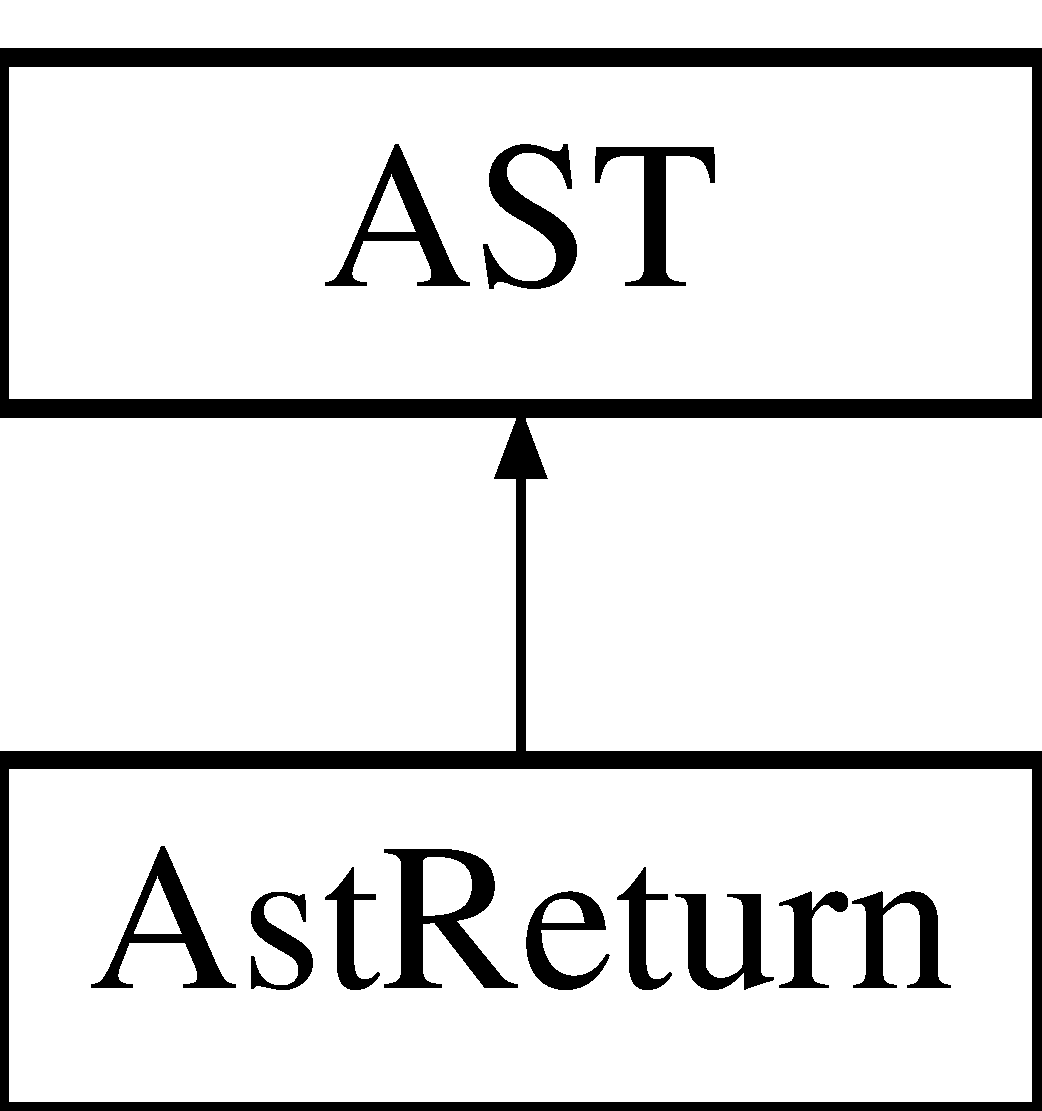
\includegraphics[height=2.000000cm]{classAstReturn}
\end{center}
\end{figure}
\subsection*{Public Member Functions}
\begin{DoxyCompactItemize}
\item 
\hypertarget{classAstReturn_a8501045c949a42680c1fe7553473fc8a}{{\bfseries Ast\-Return} (\hyperlink{classAstExpression}{Ast\-Expression} $\ast$r)}\label{classAstReturn_a8501045c949a42680c1fe7553473fc8a}

\item 
void \hyperlink{classAstReturn_a220df2fba1ee6802b89f55d16821b6ea}{Visit} ()
\begin{DoxyCompactList}\small\item\em This function is responsible for tree traversals. \end{DoxyCompactList}\item 
\hypertarget{classAstReturn_a8501045c949a42680c1fe7553473fc8a}{{\bfseries Ast\-Return} (\hyperlink{classAstExpression}{Ast\-Expression} $\ast$r)}\label{classAstReturn_a8501045c949a42680c1fe7553473fc8a}

\item 
void \hyperlink{classAstReturn_a220df2fba1ee6802b89f55d16821b6ea}{Visit} ()
\begin{DoxyCompactList}\small\item\em This function is responsible for tree traversals. \end{DoxyCompactList}\item 
\hypertarget{classAstReturn_a8501045c949a42680c1fe7553473fc8a}{{\bfseries Ast\-Return} (\hyperlink{classAstExpression}{Ast\-Expression} $\ast$r)}\label{classAstReturn_a8501045c949a42680c1fe7553473fc8a}

\item 
void \hyperlink{classAstReturn_a220df2fba1ee6802b89f55d16821b6ea}{Visit} ()
\begin{DoxyCompactList}\small\item\em This function is responsible for tree traversals. \end{DoxyCompactList}\item 
\hypertarget{classAstReturn_a8501045c949a42680c1fe7553473fc8a}{{\bfseries Ast\-Return} (\hyperlink{classAstExpression}{Ast\-Expression} $\ast$r)}\label{classAstReturn_a8501045c949a42680c1fe7553473fc8a}

\item 
void \hyperlink{classAstReturn_a220df2fba1ee6802b89f55d16821b6ea}{Visit} ()
\begin{DoxyCompactList}\small\item\em This function is responsible for tree traversals. \end{DoxyCompactList}\item 
void \hyperlink{classAST_a71d680856e95ff89f55d5311a552eba6}{set\-Label} (string l)
\begin{DoxyCompactList}\small\item\em Sets the label for the node. \end{DoxyCompactList}\item 
void \hyperlink{classAST_a71d680856e95ff89f55d5311a552eba6}{set\-Label} (string l)
\begin{DoxyCompactList}\small\item\em Sets the label for the node. \end{DoxyCompactList}\item 
void \hyperlink{classAST_a71d680856e95ff89f55d5311a552eba6}{set\-Label} (string l)
\begin{DoxyCompactList}\small\item\em Sets the label for the node. \end{DoxyCompactList}\item 
void \hyperlink{classAST_a71d680856e95ff89f55d5311a552eba6}{set\-Label} (string l)
\begin{DoxyCompactList}\small\item\em Sets the label for the node. \end{DoxyCompactList}\item 
int \hyperlink{classAST_ab7a5b1d9f1c2de0d98deb356f724a42c}{get\-U\-I\-D} ()
\begin{DoxyCompactList}\small\item\em Gets the node's unique I\-D. \end{DoxyCompactList}\item 
int \hyperlink{classAST_ab7a5b1d9f1c2de0d98deb356f724a42c}{get\-U\-I\-D} ()
\begin{DoxyCompactList}\small\item\em Gets the node's unique I\-D. \end{DoxyCompactList}\item 
int \hyperlink{classAST_ab7a5b1d9f1c2de0d98deb356f724a42c}{get\-U\-I\-D} ()
\begin{DoxyCompactList}\small\item\em Gets the node's unique I\-D. \end{DoxyCompactList}\item 
int \hyperlink{classAST_ab7a5b1d9f1c2de0d98deb356f724a42c}{get\-U\-I\-D} ()
\begin{DoxyCompactList}\small\item\em Gets the node's unique I\-D. \end{DoxyCompactList}\item 
string \hyperlink{classAST_aee029be902fffc927d16ccb03eb922ad}{get\-Label} ()
\begin{DoxyCompactList}\small\item\em Gets the node's label. \end{DoxyCompactList}\item 
string \hyperlink{classAST_aee029be902fffc927d16ccb03eb922ad}{get\-Label} ()
\begin{DoxyCompactList}\small\item\em Gets the node's label. \end{DoxyCompactList}\item 
string \hyperlink{classAST_aee029be902fffc927d16ccb03eb922ad}{get\-Label} ()
\begin{DoxyCompactList}\small\item\em Gets the node's label. \end{DoxyCompactList}\item 
string \hyperlink{classAST_aee029be902fffc927d16ccb03eb922ad}{get\-Label} ()
\begin{DoxyCompactList}\small\item\em Gets the node's label. \end{DoxyCompactList}\end{DoxyCompactItemize}
\subsection*{Public Attributes}
\begin{DoxyCompactItemize}
\item 
\hypertarget{classAST_aaf215802de409f8096c063d01ffa6783}{bool \hyperlink{classAST_aaf215802de409f8096c063d01ffa6783}{needs\-Cast}}\label{classAST_aaf215802de409f8096c063d01ffa6783}

\begin{DoxyCompactList}\small\item\em This indicates if cast 3\-A\-C needs to be output, and is only relevant for expressions. \end{DoxyCompactList}\item 
\hypertarget{classAST_afa9e77ef650ec6664458fa6cb55be985}{bool \hyperlink{classAST_afa9e77ef650ec6664458fa6cb55be985}{is\-Conv}}\label{classAST_afa9e77ef650ec6664458fa6cb55be985}

\begin{DoxyCompactList}\small\item\em Indicates is a conversion is possible. \end{DoxyCompactList}\item 
\hypertarget{classAST_a61ef3317e023d45237e06615b387cd6b}{C\-O\-N\-V\-E\-R\-S\-I\-O\-N\-T\-Y\-P\-E \hyperlink{classAST_a61ef3317e023d45237e06615b387cd6b}{conv\-Type}}\label{classAST_a61ef3317e023d45237e06615b387cd6b}

\begin{DoxyCompactList}\small\item\em If needs\-Cast is true, then this indicates what the cast should be. \end{DoxyCompactList}\item 
\hypertarget{classAST_aea9b07b39d24183f38c0029cec0a878e}{int \hyperlink{classAST_aea9b07b39d24183f38c0029cec0a878e}{operand\-To\-Cast}}\label{classAST_aea9b07b39d24183f38c0029cec0a878e}

\begin{DoxyCompactList}\small\item\em This indicates if the first or second operand should be the one that is cast. \end{DoxyCompactList}\end{DoxyCompactItemize}
\subsection*{Static Public Attributes}
\begin{DoxyCompactItemize}
\item 
\hypertarget{classAST_a5fdfd5f7b104dd92889163bdadbc68d6}{static \hyperlink{classVisualizer}{Visualizer} \hyperlink{classAST_a5fdfd5f7b104dd92889163bdadbc68d6}{vis}}\label{classAST_a5fdfd5f7b104dd92889163bdadbc68d6}

\begin{DoxyCompactList}\small\item\em Static visualizer instance for generating the visualization of the \hyperlink{classAST}{A\-S\-T}. \end{DoxyCompactList}\item 
\hypertarget{classAST_a8a3ace322f50e030331065d644ee55ee}{static \hyperlink{classTAC__Generator}{T\-A\-C\-\_\-\-Generator} \hyperlink{classAST_a8a3ace322f50e030331065d644ee55ee}{tac\-Gen}}\label{classAST_a8a3ace322f50e030331065d644ee55ee}

\begin{DoxyCompactList}\small\item\em Three address code generator. \end{DoxyCompactList}\item 
\hypertarget{classAST_a1f69448c6dc368d005631a128460083d}{static string {\bfseries current\-Temp} =\char`\"{}\char`\"{}}\label{classAST_a1f69448c6dc368d005631a128460083d}

\item 
\hypertarget{classAST_a551aec090c932ab69365238b40a8a4eb}{static string \hyperlink{classAST_a551aec090c932ab69365238b40a8a4eb}{return\-Label} =\char`\"{}\char`\"{}}\label{classAST_a551aec090c932ab69365238b40a8a4eb}

\begin{DoxyCompactList}\small\item\em This is for storing the string id of any temporary result register that may be created during 3\-A\-C generation. \end{DoxyCompactList}\item 
\hypertarget{classAST_a73c0a266df52be71e6b527b6aa635173}{static list$<$ string $>$ {\bfseries temp\-Stack}}\label{classAST_a73c0a266df52be71e6b527b6aa635173}

\item 
\hypertarget{classAST_abf9e84b541ff04b7bb64e6e4371512d4}{static string {\bfseries last\-I\-D} =\char`\"{}\char`\"{}}\label{classAST_abf9e84b541ff04b7bb64e6e4371512d4}

\item 
\hypertarget{classAST_a163003bfe9c30510ec8039870346049f}{static \hyperlink{classSymTab}{Sym\-Tab} $\ast$ {\bfseries symbol\-Table} =N\-U\-L\-L}\label{classAST_a163003bfe9c30510ec8039870346049f}

\item 
\hypertarget{classAST_a5c3cc894d9c0453523dec9ed76f18a04}{static string {\bfseries current\-Function} =\char`\"{}\char`\"{}}\label{classAST_a5c3cc894d9c0453523dec9ed76f18a04}

\end{DoxyCompactItemize}
\subsection*{Protected Attributes}
\begin{DoxyCompactItemize}
\item 
\hypertarget{classAST_a847b778f1c3dd5a19de32de432ee6e15}{int \hyperlink{classAST_a847b778f1c3dd5a19de32de432ee6e15}{uid}}\label{classAST_a847b778f1c3dd5a19de32de432ee6e15}

\begin{DoxyCompactList}\small\item\em The unique id. \end{DoxyCompactList}\item 
\hypertarget{classAST_ab2e239ccc0688d2341724432ff5a1a31}{string \hyperlink{classAST_ab2e239ccc0688d2341724432ff5a1a31}{label}}\label{classAST_ab2e239ccc0688d2341724432ff5a1a31}

\begin{DoxyCompactList}\small\item\em The label to be printed in the visualization. \end{DoxyCompactList}\end{DoxyCompactItemize}
\subsection*{Private Attributes}
\begin{DoxyCompactItemize}
\item 
\hypertarget{classAstReturn_ad42e6ca1a060c64df0660fcf3e915ea2}{\hyperlink{classAstExpression}{Ast\-Expression} $\ast$ {\bfseries expr}}\label{classAstReturn_ad42e6ca1a060c64df0660fcf3e915ea2}

\end{DoxyCompactItemize}


\subsection{Detailed Description}


Definition at line 641 of file Ast.\-h.



\subsection{Member Function Documentation}
\hypertarget{classAST_aee029be902fffc927d16ccb03eb922ad}{\index{Ast\-Return@{Ast\-Return}!get\-Label@{get\-Label}}
\index{get\-Label@{get\-Label}!AstReturn@{Ast\-Return}}
\subsubsection[{get\-Label}]{\setlength{\rightskip}{0pt plus 5cm}string A\-S\-T\-::get\-Label (
\begin{DoxyParamCaption}
{}
\end{DoxyParamCaption}
)\hspace{0.3cm}{\ttfamily [inline]}, {\ttfamily [inherited]}}}\label{classAST_aee029be902fffc927d16ccb03eb922ad}


Gets the node's label. 

\begin{DoxyReturn}{Returns}
The label 
\end{DoxyReturn}


Definition at line 60 of file Ast.\-h.

\hypertarget{classAST_aee029be902fffc927d16ccb03eb922ad}{\index{Ast\-Return@{Ast\-Return}!get\-Label@{get\-Label}}
\index{get\-Label@{get\-Label}!AstReturn@{Ast\-Return}}
\subsubsection[{get\-Label}]{\setlength{\rightskip}{0pt plus 5cm}string A\-S\-T\-::get\-Label (
\begin{DoxyParamCaption}
{}
\end{DoxyParamCaption}
)\hspace{0.3cm}{\ttfamily [inline]}, {\ttfamily [inherited]}}}\label{classAST_aee029be902fffc927d16ccb03eb922ad}


Gets the node's label. 

\begin{DoxyReturn}{Returns}
The label 
\end{DoxyReturn}


Definition at line 60 of file C\-Scanner.\-ll.

\hypertarget{classAST_aee029be902fffc927d16ccb03eb922ad}{\index{Ast\-Return@{Ast\-Return}!get\-Label@{get\-Label}}
\index{get\-Label@{get\-Label}!AstReturn@{Ast\-Return}}
\subsubsection[{get\-Label}]{\setlength{\rightskip}{0pt plus 5cm}string A\-S\-T\-::get\-Label (
\begin{DoxyParamCaption}
{}
\end{DoxyParamCaption}
)\hspace{0.3cm}{\ttfamily [inline]}, {\ttfamily [inherited]}}}\label{classAST_aee029be902fffc927d16ccb03eb922ad}


Gets the node's label. 

\begin{DoxyReturn}{Returns}
The label 
\end{DoxyReturn}


Definition at line 60 of file C\-Parser.\-yy.

\hypertarget{classAST_aee029be902fffc927d16ccb03eb922ad}{\index{Ast\-Return@{Ast\-Return}!get\-Label@{get\-Label}}
\index{get\-Label@{get\-Label}!AstReturn@{Ast\-Return}}
\subsubsection[{get\-Label}]{\setlength{\rightskip}{0pt plus 5cm}string A\-S\-T\-::get\-Label (
\begin{DoxyParamCaption}
{}
\end{DoxyParamCaption}
)\hspace{0.3cm}{\ttfamily [inline]}, {\ttfamily [inherited]}}}\label{classAST_aee029be902fffc927d16ccb03eb922ad}


Gets the node's label. 

\begin{DoxyReturn}{Returns}
The label 
\end{DoxyReturn}


Definition at line 60 of file C\-Parser.\-yy.

\hypertarget{classAST_ab7a5b1d9f1c2de0d98deb356f724a42c}{\index{Ast\-Return@{Ast\-Return}!get\-U\-I\-D@{get\-U\-I\-D}}
\index{get\-U\-I\-D@{get\-U\-I\-D}!AstReturn@{Ast\-Return}}
\subsubsection[{get\-U\-I\-D}]{\setlength{\rightskip}{0pt plus 5cm}int A\-S\-T\-::get\-U\-I\-D (
\begin{DoxyParamCaption}
{}
\end{DoxyParamCaption}
)\hspace{0.3cm}{\ttfamily [inline]}, {\ttfamily [inherited]}}}\label{classAST_ab7a5b1d9f1c2de0d98deb356f724a42c}


Gets the node's unique I\-D. 

\begin{DoxyReturn}{Returns}
The unique id 
\end{DoxyReturn}


Definition at line 53 of file C\-Parser.\-yy.

\hypertarget{classAST_ab7a5b1d9f1c2de0d98deb356f724a42c}{\index{Ast\-Return@{Ast\-Return}!get\-U\-I\-D@{get\-U\-I\-D}}
\index{get\-U\-I\-D@{get\-U\-I\-D}!AstReturn@{Ast\-Return}}
\subsubsection[{get\-U\-I\-D}]{\setlength{\rightskip}{0pt plus 5cm}int A\-S\-T\-::get\-U\-I\-D (
\begin{DoxyParamCaption}
{}
\end{DoxyParamCaption}
)\hspace{0.3cm}{\ttfamily [inline]}, {\ttfamily [inherited]}}}\label{classAST_ab7a5b1d9f1c2de0d98deb356f724a42c}


Gets the node's unique I\-D. 

\begin{DoxyReturn}{Returns}
The unique id 
\end{DoxyReturn}


Definition at line 53 of file C\-Parser.\-yy.

\hypertarget{classAST_ab7a5b1d9f1c2de0d98deb356f724a42c}{\index{Ast\-Return@{Ast\-Return}!get\-U\-I\-D@{get\-U\-I\-D}}
\index{get\-U\-I\-D@{get\-U\-I\-D}!AstReturn@{Ast\-Return}}
\subsubsection[{get\-U\-I\-D}]{\setlength{\rightskip}{0pt plus 5cm}int A\-S\-T\-::get\-U\-I\-D (
\begin{DoxyParamCaption}
{}
\end{DoxyParamCaption}
)\hspace{0.3cm}{\ttfamily [inline]}, {\ttfamily [inherited]}}}\label{classAST_ab7a5b1d9f1c2de0d98deb356f724a42c}


Gets the node's unique I\-D. 

\begin{DoxyReturn}{Returns}
The unique id 
\end{DoxyReturn}


Definition at line 53 of file C\-Scanner.\-ll.

\hypertarget{classAST_ab7a5b1d9f1c2de0d98deb356f724a42c}{\index{Ast\-Return@{Ast\-Return}!get\-U\-I\-D@{get\-U\-I\-D}}
\index{get\-U\-I\-D@{get\-U\-I\-D}!AstReturn@{Ast\-Return}}
\subsubsection[{get\-U\-I\-D}]{\setlength{\rightskip}{0pt plus 5cm}int A\-S\-T\-::get\-U\-I\-D (
\begin{DoxyParamCaption}
{}
\end{DoxyParamCaption}
)\hspace{0.3cm}{\ttfamily [inline]}, {\ttfamily [inherited]}}}\label{classAST_ab7a5b1d9f1c2de0d98deb356f724a42c}


Gets the node's unique I\-D. 

\begin{DoxyReturn}{Returns}
The unique id 
\end{DoxyReturn}


Definition at line 53 of file Ast.\-h.

\hypertarget{classAST_a71d680856e95ff89f55d5311a552eba6}{\index{Ast\-Return@{Ast\-Return}!set\-Label@{set\-Label}}
\index{set\-Label@{set\-Label}!AstReturn@{Ast\-Return}}
\subsubsection[{set\-Label}]{\setlength{\rightskip}{0pt plus 5cm}void A\-S\-T\-::set\-Label (
\begin{DoxyParamCaption}
\item[{string}]{l}
\end{DoxyParamCaption}
)\hspace{0.3cm}{\ttfamily [inline]}, {\ttfamily [inherited]}}}\label{classAST_a71d680856e95ff89f55d5311a552eba6}


Sets the label for the node. 


\begin{DoxyParams}{Parameters}
{\em l} & The label string \\
\hline
\end{DoxyParams}


Definition at line 43 of file C\-Scanner.\-ll.

\hypertarget{classAST_a71d680856e95ff89f55d5311a552eba6}{\index{Ast\-Return@{Ast\-Return}!set\-Label@{set\-Label}}
\index{set\-Label@{set\-Label}!AstReturn@{Ast\-Return}}
\subsubsection[{set\-Label}]{\setlength{\rightskip}{0pt plus 5cm}void A\-S\-T\-::set\-Label (
\begin{DoxyParamCaption}
\item[{string}]{l}
\end{DoxyParamCaption}
)\hspace{0.3cm}{\ttfamily [inline]}, {\ttfamily [inherited]}}}\label{classAST_a71d680856e95ff89f55d5311a552eba6}


Sets the label for the node. 


\begin{DoxyParams}{Parameters}
{\em l} & The label string \\
\hline
\end{DoxyParams}


Definition at line 43 of file C\-Parser.\-yy.

\hypertarget{classAST_a71d680856e95ff89f55d5311a552eba6}{\index{Ast\-Return@{Ast\-Return}!set\-Label@{set\-Label}}
\index{set\-Label@{set\-Label}!AstReturn@{Ast\-Return}}
\subsubsection[{set\-Label}]{\setlength{\rightskip}{0pt plus 5cm}void A\-S\-T\-::set\-Label (
\begin{DoxyParamCaption}
\item[{string}]{l}
\end{DoxyParamCaption}
)\hspace{0.3cm}{\ttfamily [inline]}, {\ttfamily [inherited]}}}\label{classAST_a71d680856e95ff89f55d5311a552eba6}


Sets the label for the node. 


\begin{DoxyParams}{Parameters}
{\em l} & The label string \\
\hline
\end{DoxyParams}


Definition at line 43 of file Ast.\-h.

\hypertarget{classAST_a71d680856e95ff89f55d5311a552eba6}{\index{Ast\-Return@{Ast\-Return}!set\-Label@{set\-Label}}
\index{set\-Label@{set\-Label}!AstReturn@{Ast\-Return}}
\subsubsection[{set\-Label}]{\setlength{\rightskip}{0pt plus 5cm}void A\-S\-T\-::set\-Label (
\begin{DoxyParamCaption}
\item[{string}]{l}
\end{DoxyParamCaption}
)\hspace{0.3cm}{\ttfamily [inline]}, {\ttfamily [inherited]}}}\label{classAST_a71d680856e95ff89f55d5311a552eba6}


Sets the label for the node. 


\begin{DoxyParams}{Parameters}
{\em l} & The label string \\
\hline
\end{DoxyParams}


Definition at line 43 of file C\-Parser.\-yy.

\hypertarget{classAstReturn_a220df2fba1ee6802b89f55d16821b6ea}{\index{Ast\-Return@{Ast\-Return}!Visit@{Visit}}
\index{Visit@{Visit}!AstReturn@{Ast\-Return}}
\subsubsection[{Visit}]{\setlength{\rightskip}{0pt plus 5cm}void Ast\-Return\-::\-Visit (
\begin{DoxyParamCaption}
{}
\end{DoxyParamCaption}
)\hspace{0.3cm}{\ttfamily [virtual]}}}\label{classAstReturn_a220df2fba1ee6802b89f55d16821b6ea}


This function is responsible for tree traversals. 

This function will call the Visit functions of each of it's children nodes, call the visualization code for itself, and output any 3\-A\-C that can be generated at the current node. 

Reimplemented from \hyperlink{classAST_a5828cc86f2c4f1a0aeab6d7069e8fd82}{A\-S\-T}.



Definition at line 1888 of file Ast.\-cpp.

\hypertarget{classAstReturn_a220df2fba1ee6802b89f55d16821b6ea}{\index{Ast\-Return@{Ast\-Return}!Visit@{Visit}}
\index{Visit@{Visit}!AstReturn@{Ast\-Return}}
\subsubsection[{Visit}]{\setlength{\rightskip}{0pt plus 5cm}void Ast\-Return\-::\-Visit (
\begin{DoxyParamCaption}
{}
\end{DoxyParamCaption}
)\hspace{0.3cm}{\ttfamily [virtual]}}}\label{classAstReturn_a220df2fba1ee6802b89f55d16821b6ea}


This function is responsible for tree traversals. 

This function will call the Visit functions of each of it's children nodes, call the visualization code for itself, and output any 3\-A\-C that can be generated at the current node. 

Reimplemented from \hyperlink{classAST_a5828cc86f2c4f1a0aeab6d7069e8fd82}{A\-S\-T}.

\hypertarget{classAstReturn_a220df2fba1ee6802b89f55d16821b6ea}{\index{Ast\-Return@{Ast\-Return}!Visit@{Visit}}
\index{Visit@{Visit}!AstReturn@{Ast\-Return}}
\subsubsection[{Visit}]{\setlength{\rightskip}{0pt plus 5cm}void Ast\-Return\-::\-Visit (
\begin{DoxyParamCaption}
{}
\end{DoxyParamCaption}
)\hspace{0.3cm}{\ttfamily [virtual]}}}\label{classAstReturn_a220df2fba1ee6802b89f55d16821b6ea}


This function is responsible for tree traversals. 

This function will call the Visit functions of each of it's children nodes, call the visualization code for itself, and output any 3\-A\-C that can be generated at the current node. 

Reimplemented from \hyperlink{classAST_a5828cc86f2c4f1a0aeab6d7069e8fd82}{A\-S\-T}.

\hypertarget{classAstReturn_a220df2fba1ee6802b89f55d16821b6ea}{\index{Ast\-Return@{Ast\-Return}!Visit@{Visit}}
\index{Visit@{Visit}!AstReturn@{Ast\-Return}}
\subsubsection[{Visit}]{\setlength{\rightskip}{0pt plus 5cm}void Ast\-Return\-::\-Visit (
\begin{DoxyParamCaption}
{}
\end{DoxyParamCaption}
)\hspace{0.3cm}{\ttfamily [virtual]}}}\label{classAstReturn_a220df2fba1ee6802b89f55d16821b6ea}


This function is responsible for tree traversals. 

This function will call the Visit functions of each of it's children nodes, call the visualization code for itself, and output any 3\-A\-C that can be generated at the current node. 

Reimplemented from \hyperlink{classAST_a5828cc86f2c4f1a0aeab6d7069e8fd82}{A\-S\-T}.



The documentation for this class was generated from the following files\-:\begin{DoxyCompactItemize}
\item 
Ast.\-h\item 
Ast.\-cpp\end{DoxyCompactItemize}

\hypertarget{classAstSelection}{\section{Ast\-Selection Class Reference}
\label{classAstSelection}\index{Ast\-Selection@{Ast\-Selection}}
}
Inheritance diagram for Ast\-Selection\-:\begin{figure}[H]
\begin{center}
\leavevmode
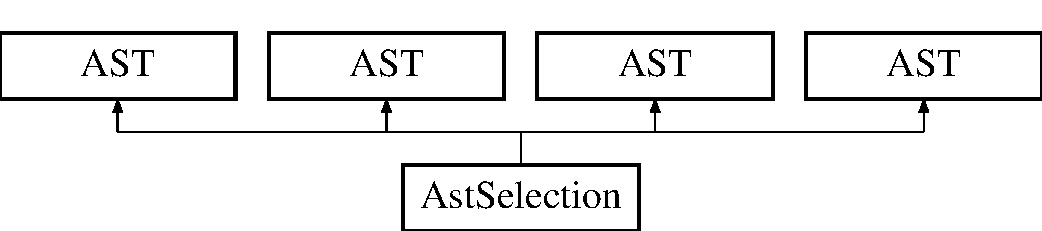
\includegraphics[height=2.000000cm]{classAstSelection}
\end{center}
\end{figure}
\subsection*{Public Types}
\begin{DoxyCompactItemize}
\item 
enum {\bfseries Type} \{ \\*
{\bfseries S\-W\-I\-T\-C\-H}, 
{\bfseries I\-F\-E\-L\-S\-E}, 
{\bfseries S\-W\-I\-T\-C\-H}, 
{\bfseries I\-F\-E\-L\-S\-E}, 
\\*
{\bfseries S\-W\-I\-T\-C\-H}, 
{\bfseries I\-F\-E\-L\-S\-E}, 
{\bfseries S\-W\-I\-T\-C\-H}, 
{\bfseries I\-F\-E\-L\-S\-E}
 \}
\item 
enum {\bfseries Type} \{ \\*
{\bfseries S\-W\-I\-T\-C\-H}, 
{\bfseries I\-F\-E\-L\-S\-E}, 
{\bfseries S\-W\-I\-T\-C\-H}, 
{\bfseries I\-F\-E\-L\-S\-E}, 
\\*
{\bfseries S\-W\-I\-T\-C\-H}, 
{\bfseries I\-F\-E\-L\-S\-E}, 
{\bfseries S\-W\-I\-T\-C\-H}, 
{\bfseries I\-F\-E\-L\-S\-E}
 \}
\item 
enum {\bfseries Type} \{ \\*
{\bfseries S\-W\-I\-T\-C\-H}, 
{\bfseries I\-F\-E\-L\-S\-E}, 
{\bfseries S\-W\-I\-T\-C\-H}, 
{\bfseries I\-F\-E\-L\-S\-E}, 
\\*
{\bfseries S\-W\-I\-T\-C\-H}, 
{\bfseries I\-F\-E\-L\-S\-E}, 
{\bfseries S\-W\-I\-T\-C\-H}, 
{\bfseries I\-F\-E\-L\-S\-E}
 \}
\item 
enum {\bfseries Type} \{ \\*
{\bfseries S\-W\-I\-T\-C\-H}, 
{\bfseries I\-F\-E\-L\-S\-E}, 
{\bfseries S\-W\-I\-T\-C\-H}, 
{\bfseries I\-F\-E\-L\-S\-E}, 
\\*
{\bfseries S\-W\-I\-T\-C\-H}, 
{\bfseries I\-F\-E\-L\-S\-E}, 
{\bfseries S\-W\-I\-T\-C\-H}, 
{\bfseries I\-F\-E\-L\-S\-E}
 \}
\end{DoxyCompactItemize}
\subsection*{Public Member Functions}
\begin{DoxyCompactItemize}
\item 
\hypertarget{classAstSelection_afac2e382bc352b49ca61e6017eb58130}{{\bfseries Ast\-Selection} (\hyperlink{classAstSwitch}{Ast\-Switch} $\ast$s)}\label{classAstSelection_afac2e382bc352b49ca61e6017eb58130}

\item 
\hypertarget{classAstSelection_aaed7d12c4b620b13f70e2d19e15eff0c}{{\bfseries Ast\-Selection} (\hyperlink{classAstIfElse}{Ast\-If\-Else} $\ast$ie)}\label{classAstSelection_aaed7d12c4b620b13f70e2d19e15eff0c}

\item 
void \hyperlink{classAstSelection_a811114a424918b2141b5eb0e341c3a22}{Visit} ()
\begin{DoxyCompactList}\small\item\em This function is responsible for tree traversals. \end{DoxyCompactList}\item 
\hypertarget{classAstSelection_afac2e382bc352b49ca61e6017eb58130}{{\bfseries Ast\-Selection} (\hyperlink{classAstSwitch}{Ast\-Switch} $\ast$s)}\label{classAstSelection_afac2e382bc352b49ca61e6017eb58130}

\item 
\hypertarget{classAstSelection_aaed7d12c4b620b13f70e2d19e15eff0c}{{\bfseries Ast\-Selection} (\hyperlink{classAstIfElse}{Ast\-If\-Else} $\ast$ie)}\label{classAstSelection_aaed7d12c4b620b13f70e2d19e15eff0c}

\item 
void \hyperlink{classAstSelection_a811114a424918b2141b5eb0e341c3a22}{Visit} ()
\begin{DoxyCompactList}\small\item\em This function is responsible for tree traversals. \end{DoxyCompactList}\item 
\hypertarget{classAstSelection_afac2e382bc352b49ca61e6017eb58130}{{\bfseries Ast\-Selection} (\hyperlink{classAstSwitch}{Ast\-Switch} $\ast$s)}\label{classAstSelection_afac2e382bc352b49ca61e6017eb58130}

\item 
\hypertarget{classAstSelection_aaed7d12c4b620b13f70e2d19e15eff0c}{{\bfseries Ast\-Selection} (\hyperlink{classAstIfElse}{Ast\-If\-Else} $\ast$ie)}\label{classAstSelection_aaed7d12c4b620b13f70e2d19e15eff0c}

\item 
void \hyperlink{classAstSelection_a811114a424918b2141b5eb0e341c3a22}{Visit} ()
\begin{DoxyCompactList}\small\item\em This function is responsible for tree traversals. \end{DoxyCompactList}\item 
\hypertarget{classAstSelection_afac2e382bc352b49ca61e6017eb58130}{{\bfseries Ast\-Selection} (\hyperlink{classAstSwitch}{Ast\-Switch} $\ast$s)}\label{classAstSelection_afac2e382bc352b49ca61e6017eb58130}

\item 
\hypertarget{classAstSelection_aaed7d12c4b620b13f70e2d19e15eff0c}{{\bfseries Ast\-Selection} (\hyperlink{classAstIfElse}{Ast\-If\-Else} $\ast$ie)}\label{classAstSelection_aaed7d12c4b620b13f70e2d19e15eff0c}

\item 
void \hyperlink{classAstSelection_a811114a424918b2141b5eb0e341c3a22}{Visit} ()
\begin{DoxyCompactList}\small\item\em This function is responsible for tree traversals. \end{DoxyCompactList}\item 
void \hyperlink{classAST_a71d680856e95ff89f55d5311a552eba6}{set\-Label} (string l)
\begin{DoxyCompactList}\small\item\em Sets the label for the node. \end{DoxyCompactList}\item 
void \hyperlink{classAST_a71d680856e95ff89f55d5311a552eba6}{set\-Label} (string l)
\begin{DoxyCompactList}\small\item\em Sets the label for the node. \end{DoxyCompactList}\item 
void \hyperlink{classAST_a71d680856e95ff89f55d5311a552eba6}{set\-Label} (string l)
\begin{DoxyCompactList}\small\item\em Sets the label for the node. \end{DoxyCompactList}\item 
void \hyperlink{classAST_a71d680856e95ff89f55d5311a552eba6}{set\-Label} (string l)
\begin{DoxyCompactList}\small\item\em Sets the label for the node. \end{DoxyCompactList}\item 
int \hyperlink{classAST_ab7a5b1d9f1c2de0d98deb356f724a42c}{get\-U\-I\-D} ()
\begin{DoxyCompactList}\small\item\em Gets the node's unique I\-D. \end{DoxyCompactList}\item 
int \hyperlink{classAST_ab7a5b1d9f1c2de0d98deb356f724a42c}{get\-U\-I\-D} ()
\begin{DoxyCompactList}\small\item\em Gets the node's unique I\-D. \end{DoxyCompactList}\item 
int \hyperlink{classAST_ab7a5b1d9f1c2de0d98deb356f724a42c}{get\-U\-I\-D} ()
\begin{DoxyCompactList}\small\item\em Gets the node's unique I\-D. \end{DoxyCompactList}\item 
int \hyperlink{classAST_ab7a5b1d9f1c2de0d98deb356f724a42c}{get\-U\-I\-D} ()
\begin{DoxyCompactList}\small\item\em Gets the node's unique I\-D. \end{DoxyCompactList}\item 
string \hyperlink{classAST_aee029be902fffc927d16ccb03eb922ad}{get\-Label} ()
\begin{DoxyCompactList}\small\item\em Gets the node's label. \end{DoxyCompactList}\item 
string \hyperlink{classAST_aee029be902fffc927d16ccb03eb922ad}{get\-Label} ()
\begin{DoxyCompactList}\small\item\em Gets the node's label. \end{DoxyCompactList}\item 
string \hyperlink{classAST_aee029be902fffc927d16ccb03eb922ad}{get\-Label} ()
\begin{DoxyCompactList}\small\item\em Gets the node's label. \end{DoxyCompactList}\item 
string \hyperlink{classAST_aee029be902fffc927d16ccb03eb922ad}{get\-Label} ()
\begin{DoxyCompactList}\small\item\em Gets the node's label. \end{DoxyCompactList}\end{DoxyCompactItemize}
\subsection*{Public Attributes}
\begin{DoxyCompactItemize}
\item 
\hypertarget{classAstSelection_a638d589f77696ed1d0df98aaa0e50835}{enum Ast\-Selection\-::\-Type {\bfseries t}}\label{classAstSelection_a638d589f77696ed1d0df98aaa0e50835}

\item 
\hypertarget{classAST_aaf215802de409f8096c063d01ffa6783}{bool \hyperlink{classAST_aaf215802de409f8096c063d01ffa6783}{needs\-Cast}}\label{classAST_aaf215802de409f8096c063d01ffa6783}

\begin{DoxyCompactList}\small\item\em This indicates if cast 3\-A\-C needs to be output, and is only relevant for expressions. \end{DoxyCompactList}\item 
\hypertarget{classAST_afa9e77ef650ec6664458fa6cb55be985}{bool \hyperlink{classAST_afa9e77ef650ec6664458fa6cb55be985}{is\-Conv}}\label{classAST_afa9e77ef650ec6664458fa6cb55be985}

\begin{DoxyCompactList}\small\item\em Indicates is a conversion is possible. \end{DoxyCompactList}\item 
\hypertarget{classAST_a61ef3317e023d45237e06615b387cd6b}{C\-O\-N\-V\-E\-R\-S\-I\-O\-N\-T\-Y\-P\-E \hyperlink{classAST_a61ef3317e023d45237e06615b387cd6b}{conv\-Type}}\label{classAST_a61ef3317e023d45237e06615b387cd6b}

\begin{DoxyCompactList}\small\item\em If needs\-Cast is true, then this indicates what the cast should be. \end{DoxyCompactList}\item 
\hypertarget{classAST_aea9b07b39d24183f38c0029cec0a878e}{int \hyperlink{classAST_aea9b07b39d24183f38c0029cec0a878e}{operand\-To\-Cast}}\label{classAST_aea9b07b39d24183f38c0029cec0a878e}

\begin{DoxyCompactList}\small\item\em This indicates if the first or second operand should be the one that is cast. \end{DoxyCompactList}\end{DoxyCompactItemize}
\subsection*{Static Public Attributes}
\begin{DoxyCompactItemize}
\item 
\hypertarget{classAST_a5fdfd5f7b104dd92889163bdadbc68d6}{static \hyperlink{classVisualizer}{Visualizer} \hyperlink{classAST_a5fdfd5f7b104dd92889163bdadbc68d6}{vis}}\label{classAST_a5fdfd5f7b104dd92889163bdadbc68d6}

\begin{DoxyCompactList}\small\item\em Static visualizer instance for generating the visualization of the \hyperlink{classAST}{A\-S\-T}. \end{DoxyCompactList}\item 
\hypertarget{classAST_a8a3ace322f50e030331065d644ee55ee}{static \hyperlink{classTAC__Generator}{T\-A\-C\-\_\-\-Generator} \hyperlink{classAST_a8a3ace322f50e030331065d644ee55ee}{tac\-Gen}}\label{classAST_a8a3ace322f50e030331065d644ee55ee}

\begin{DoxyCompactList}\small\item\em Three address code generator. \end{DoxyCompactList}\item 
\hypertarget{classAST_a1f69448c6dc368d005631a128460083d}{static string {\bfseries current\-Temp} =\char`\"{}\char`\"{}}\label{classAST_a1f69448c6dc368d005631a128460083d}

\item 
\hypertarget{classAST_a551aec090c932ab69365238b40a8a4eb}{static string \hyperlink{classAST_a551aec090c932ab69365238b40a8a4eb}{return\-Label} =\char`\"{}\char`\"{}}\label{classAST_a551aec090c932ab69365238b40a8a4eb}

\begin{DoxyCompactList}\small\item\em This is for storing the string id of any temporary result register that may be created during 3\-A\-C generation. \end{DoxyCompactList}\item 
\hypertarget{classAST_a73c0a266df52be71e6b527b6aa635173}{static list$<$ string $>$ {\bfseries temp\-Stack}}\label{classAST_a73c0a266df52be71e6b527b6aa635173}

\item 
\hypertarget{classAST_abf9e84b541ff04b7bb64e6e4371512d4}{static string {\bfseries last\-I\-D} =\char`\"{}\char`\"{}}\label{classAST_abf9e84b541ff04b7bb64e6e4371512d4}

\item 
\hypertarget{classAST_a163003bfe9c30510ec8039870346049f}{static \hyperlink{classSymTab}{Sym\-Tab} $\ast$ {\bfseries symbol\-Table} =N\-U\-L\-L}\label{classAST_a163003bfe9c30510ec8039870346049f}

\item 
\hypertarget{classAST_a5c3cc894d9c0453523dec9ed76f18a04}{static string {\bfseries current\-Function} =\char`\"{}\char`\"{}}\label{classAST_a5c3cc894d9c0453523dec9ed76f18a04}

\item 
\hypertarget{classAST_a66155513b59ff1a04c8ece8b20ec31f5}{static int {\bfseries current\-Constant\-Value} =0}\label{classAST_a66155513b59ff1a04c8ece8b20ec31f5}

\item 
\hypertarget{classAST_a3d031d7bab635ba1f015aade5943f40c}{static string {\bfseries current\-Id\-Name} =\char`\"{}\char`\"{}}\label{classAST_a3d031d7bab635ba1f015aade5943f40c}

\item 
\hypertarget{classAST_a16c4b6e54febc1a26b31a64a46972ef0}{static int {\bfseries current\-Index\-Val} = 0}\label{classAST_a16c4b6e54febc1a26b31a64a46972ef0}

\item 
\hypertarget{classAST_a6fc65ae9dd064a88941d4b88669b19db}{static string {\bfseries current\-I\-D} = \char`\"{}\char`\"{}}\label{classAST_a6fc65ae9dd064a88941d4b88669b19db}

\end{DoxyCompactItemize}
\subsection*{Protected Attributes}
\begin{DoxyCompactItemize}
\item 
\hypertarget{classAST_a847b778f1c3dd5a19de32de432ee6e15}{int \hyperlink{classAST_a847b778f1c3dd5a19de32de432ee6e15}{uid}}\label{classAST_a847b778f1c3dd5a19de32de432ee6e15}

\begin{DoxyCompactList}\small\item\em The unique id. \end{DoxyCompactList}\item 
\hypertarget{classAST_ab2e239ccc0688d2341724432ff5a1a31}{string \hyperlink{classAST_ab2e239ccc0688d2341724432ff5a1a31}{label}}\label{classAST_ab2e239ccc0688d2341724432ff5a1a31}

\begin{DoxyCompactList}\small\item\em The label to be printed in the visualization. \end{DoxyCompactList}\end{DoxyCompactItemize}
\subsection*{Private Attributes}
\begin{DoxyCompactItemize}
\item 
\hypertarget{classAstSelection_a2f2edb74f35f7aa53b9f26e761217e0a}{\hyperlink{classAstSwitch}{Ast\-Switch} $\ast$ {\bfseries swtch}}\label{classAstSelection_a2f2edb74f35f7aa53b9f26e761217e0a}

\item 
\hypertarget{classAstSelection_a80ba3eb140eb346ea7e4c7fb1342d41e}{\hyperlink{classAstIfElse}{Ast\-If\-Else} $\ast$ {\bfseries ifelse}}\label{classAstSelection_a80ba3eb140eb346ea7e4c7fb1342d41e}

\end{DoxyCompactItemize}


\subsection{Detailed Description}


Definition at line 928 of file Ast.\-h.



\subsection{Member Function Documentation}
\hypertarget{classAST_aee029be902fffc927d16ccb03eb922ad}{\index{Ast\-Selection@{Ast\-Selection}!get\-Label@{get\-Label}}
\index{get\-Label@{get\-Label}!AstSelection@{Ast\-Selection}}
\subsubsection[{get\-Label}]{\setlength{\rightskip}{0pt plus 5cm}string A\-S\-T\-::get\-Label (
\begin{DoxyParamCaption}
{}
\end{DoxyParamCaption}
)\hspace{0.3cm}{\ttfamily [inline]}, {\ttfamily [inherited]}}}\label{classAST_aee029be902fffc927d16ccb03eb922ad}


Gets the node's label. 

\begin{DoxyReturn}{Returns}
The label 
\end{DoxyReturn}


Definition at line 60 of file Ast.\-h.

\hypertarget{classAST_aee029be902fffc927d16ccb03eb922ad}{\index{Ast\-Selection@{Ast\-Selection}!get\-Label@{get\-Label}}
\index{get\-Label@{get\-Label}!AstSelection@{Ast\-Selection}}
\subsubsection[{get\-Label}]{\setlength{\rightskip}{0pt plus 5cm}string A\-S\-T\-::get\-Label (
\begin{DoxyParamCaption}
{}
\end{DoxyParamCaption}
)\hspace{0.3cm}{\ttfamily [inline]}, {\ttfamily [inherited]}}}\label{classAST_aee029be902fffc927d16ccb03eb922ad}


Gets the node's label. 

\begin{DoxyReturn}{Returns}
The label 
\end{DoxyReturn}


Definition at line 60 of file C\-Scanner.\-ll.

\hypertarget{classAST_aee029be902fffc927d16ccb03eb922ad}{\index{Ast\-Selection@{Ast\-Selection}!get\-Label@{get\-Label}}
\index{get\-Label@{get\-Label}!AstSelection@{Ast\-Selection}}
\subsubsection[{get\-Label}]{\setlength{\rightskip}{0pt plus 5cm}string A\-S\-T\-::get\-Label (
\begin{DoxyParamCaption}
{}
\end{DoxyParamCaption}
)\hspace{0.3cm}{\ttfamily [inline]}, {\ttfamily [inherited]}}}\label{classAST_aee029be902fffc927d16ccb03eb922ad}


Gets the node's label. 

\begin{DoxyReturn}{Returns}
The label 
\end{DoxyReturn}


Definition at line 60 of file C\-Parser.\-yy.

\hypertarget{classAST_aee029be902fffc927d16ccb03eb922ad}{\index{Ast\-Selection@{Ast\-Selection}!get\-Label@{get\-Label}}
\index{get\-Label@{get\-Label}!AstSelection@{Ast\-Selection}}
\subsubsection[{get\-Label}]{\setlength{\rightskip}{0pt plus 5cm}string A\-S\-T\-::get\-Label (
\begin{DoxyParamCaption}
{}
\end{DoxyParamCaption}
)\hspace{0.3cm}{\ttfamily [inline]}, {\ttfamily [inherited]}}}\label{classAST_aee029be902fffc927d16ccb03eb922ad}


Gets the node's label. 

\begin{DoxyReturn}{Returns}
The label 
\end{DoxyReturn}


Definition at line 60 of file C\-Parser.\-yy.

\hypertarget{classAST_ab7a5b1d9f1c2de0d98deb356f724a42c}{\index{Ast\-Selection@{Ast\-Selection}!get\-U\-I\-D@{get\-U\-I\-D}}
\index{get\-U\-I\-D@{get\-U\-I\-D}!AstSelection@{Ast\-Selection}}
\subsubsection[{get\-U\-I\-D}]{\setlength{\rightskip}{0pt plus 5cm}int A\-S\-T\-::get\-U\-I\-D (
\begin{DoxyParamCaption}
{}
\end{DoxyParamCaption}
)\hspace{0.3cm}{\ttfamily [inline]}, {\ttfamily [inherited]}}}\label{classAST_ab7a5b1d9f1c2de0d98deb356f724a42c}


Gets the node's unique I\-D. 

\begin{DoxyReturn}{Returns}
The unique id 
\end{DoxyReturn}


Definition at line 53 of file C\-Parser.\-yy.

\hypertarget{classAST_ab7a5b1d9f1c2de0d98deb356f724a42c}{\index{Ast\-Selection@{Ast\-Selection}!get\-U\-I\-D@{get\-U\-I\-D}}
\index{get\-U\-I\-D@{get\-U\-I\-D}!AstSelection@{Ast\-Selection}}
\subsubsection[{get\-U\-I\-D}]{\setlength{\rightskip}{0pt plus 5cm}int A\-S\-T\-::get\-U\-I\-D (
\begin{DoxyParamCaption}
{}
\end{DoxyParamCaption}
)\hspace{0.3cm}{\ttfamily [inline]}, {\ttfamily [inherited]}}}\label{classAST_ab7a5b1d9f1c2de0d98deb356f724a42c}


Gets the node's unique I\-D. 

\begin{DoxyReturn}{Returns}
The unique id 
\end{DoxyReturn}


Definition at line 53 of file C\-Parser.\-yy.

\hypertarget{classAST_ab7a5b1d9f1c2de0d98deb356f724a42c}{\index{Ast\-Selection@{Ast\-Selection}!get\-U\-I\-D@{get\-U\-I\-D}}
\index{get\-U\-I\-D@{get\-U\-I\-D}!AstSelection@{Ast\-Selection}}
\subsubsection[{get\-U\-I\-D}]{\setlength{\rightskip}{0pt plus 5cm}int A\-S\-T\-::get\-U\-I\-D (
\begin{DoxyParamCaption}
{}
\end{DoxyParamCaption}
)\hspace{0.3cm}{\ttfamily [inline]}, {\ttfamily [inherited]}}}\label{classAST_ab7a5b1d9f1c2de0d98deb356f724a42c}


Gets the node's unique I\-D. 

\begin{DoxyReturn}{Returns}
The unique id 
\end{DoxyReturn}


Definition at line 53 of file C\-Scanner.\-ll.

\hypertarget{classAST_ab7a5b1d9f1c2de0d98deb356f724a42c}{\index{Ast\-Selection@{Ast\-Selection}!get\-U\-I\-D@{get\-U\-I\-D}}
\index{get\-U\-I\-D@{get\-U\-I\-D}!AstSelection@{Ast\-Selection}}
\subsubsection[{get\-U\-I\-D}]{\setlength{\rightskip}{0pt plus 5cm}int A\-S\-T\-::get\-U\-I\-D (
\begin{DoxyParamCaption}
{}
\end{DoxyParamCaption}
)\hspace{0.3cm}{\ttfamily [inline]}, {\ttfamily [inherited]}}}\label{classAST_ab7a5b1d9f1c2de0d98deb356f724a42c}


Gets the node's unique I\-D. 

\begin{DoxyReturn}{Returns}
The unique id 
\end{DoxyReturn}


Definition at line 53 of file Ast.\-h.

\hypertarget{classAST_a71d680856e95ff89f55d5311a552eba6}{\index{Ast\-Selection@{Ast\-Selection}!set\-Label@{set\-Label}}
\index{set\-Label@{set\-Label}!AstSelection@{Ast\-Selection}}
\subsubsection[{set\-Label}]{\setlength{\rightskip}{0pt plus 5cm}void A\-S\-T\-::set\-Label (
\begin{DoxyParamCaption}
\item[{string}]{l}
\end{DoxyParamCaption}
)\hspace{0.3cm}{\ttfamily [inline]}, {\ttfamily [inherited]}}}\label{classAST_a71d680856e95ff89f55d5311a552eba6}


Sets the label for the node. 


\begin{DoxyParams}{Parameters}
{\em l} & The label string \\
\hline
\end{DoxyParams}


Definition at line 43 of file C\-Scanner.\-ll.

\hypertarget{classAST_a71d680856e95ff89f55d5311a552eba6}{\index{Ast\-Selection@{Ast\-Selection}!set\-Label@{set\-Label}}
\index{set\-Label@{set\-Label}!AstSelection@{Ast\-Selection}}
\subsubsection[{set\-Label}]{\setlength{\rightskip}{0pt plus 5cm}void A\-S\-T\-::set\-Label (
\begin{DoxyParamCaption}
\item[{string}]{l}
\end{DoxyParamCaption}
)\hspace{0.3cm}{\ttfamily [inline]}, {\ttfamily [inherited]}}}\label{classAST_a71d680856e95ff89f55d5311a552eba6}


Sets the label for the node. 


\begin{DoxyParams}{Parameters}
{\em l} & The label string \\
\hline
\end{DoxyParams}


Definition at line 43 of file C\-Parser.\-yy.

\hypertarget{classAST_a71d680856e95ff89f55d5311a552eba6}{\index{Ast\-Selection@{Ast\-Selection}!set\-Label@{set\-Label}}
\index{set\-Label@{set\-Label}!AstSelection@{Ast\-Selection}}
\subsubsection[{set\-Label}]{\setlength{\rightskip}{0pt plus 5cm}void A\-S\-T\-::set\-Label (
\begin{DoxyParamCaption}
\item[{string}]{l}
\end{DoxyParamCaption}
)\hspace{0.3cm}{\ttfamily [inline]}, {\ttfamily [inherited]}}}\label{classAST_a71d680856e95ff89f55d5311a552eba6}


Sets the label for the node. 


\begin{DoxyParams}{Parameters}
{\em l} & The label string \\
\hline
\end{DoxyParams}


Definition at line 43 of file Ast.\-h.

\hypertarget{classAST_a71d680856e95ff89f55d5311a552eba6}{\index{Ast\-Selection@{Ast\-Selection}!set\-Label@{set\-Label}}
\index{set\-Label@{set\-Label}!AstSelection@{Ast\-Selection}}
\subsubsection[{set\-Label}]{\setlength{\rightskip}{0pt plus 5cm}void A\-S\-T\-::set\-Label (
\begin{DoxyParamCaption}
\item[{string}]{l}
\end{DoxyParamCaption}
)\hspace{0.3cm}{\ttfamily [inline]}, {\ttfamily [inherited]}}}\label{classAST_a71d680856e95ff89f55d5311a552eba6}


Sets the label for the node. 


\begin{DoxyParams}{Parameters}
{\em l} & The label string \\
\hline
\end{DoxyParams}


Definition at line 43 of file C\-Parser.\-yy.

\hypertarget{classAstSelection_a811114a424918b2141b5eb0e341c3a22}{\index{Ast\-Selection@{Ast\-Selection}!Visit@{Visit}}
\index{Visit@{Visit}!AstSelection@{Ast\-Selection}}
\subsubsection[{Visit}]{\setlength{\rightskip}{0pt plus 5cm}void Ast\-Selection\-::\-Visit (
\begin{DoxyParamCaption}
{}
\end{DoxyParamCaption}
)\hspace{0.3cm}{\ttfamily [virtual]}}}\label{classAstSelection_a811114a424918b2141b5eb0e341c3a22}


This function is responsible for tree traversals. 

This function will call the Visit functions of each of it's children nodes, call the visualization code for itself, and output any 3\-A\-C that can be generated at the current node. 

Reimplemented from \hyperlink{classAST_a5828cc86f2c4f1a0aeab6d7069e8fd82}{A\-S\-T}.



Definition at line 2629 of file Ast.\-cpp.

\hypertarget{classAstSelection_a811114a424918b2141b5eb0e341c3a22}{\index{Ast\-Selection@{Ast\-Selection}!Visit@{Visit}}
\index{Visit@{Visit}!AstSelection@{Ast\-Selection}}
\subsubsection[{Visit}]{\setlength{\rightskip}{0pt plus 5cm}void Ast\-Selection\-::\-Visit (
\begin{DoxyParamCaption}
{}
\end{DoxyParamCaption}
)\hspace{0.3cm}{\ttfamily [virtual]}}}\label{classAstSelection_a811114a424918b2141b5eb0e341c3a22}


This function is responsible for tree traversals. 

This function will call the Visit functions of each of it's children nodes, call the visualization code for itself, and output any 3\-A\-C that can be generated at the current node. 

Reimplemented from \hyperlink{classAST_a5828cc86f2c4f1a0aeab6d7069e8fd82}{A\-S\-T}.

\hypertarget{classAstSelection_a811114a424918b2141b5eb0e341c3a22}{\index{Ast\-Selection@{Ast\-Selection}!Visit@{Visit}}
\index{Visit@{Visit}!AstSelection@{Ast\-Selection}}
\subsubsection[{Visit}]{\setlength{\rightskip}{0pt plus 5cm}void Ast\-Selection\-::\-Visit (
\begin{DoxyParamCaption}
{}
\end{DoxyParamCaption}
)\hspace{0.3cm}{\ttfamily [virtual]}}}\label{classAstSelection_a811114a424918b2141b5eb0e341c3a22}


This function is responsible for tree traversals. 

This function will call the Visit functions of each of it's children nodes, call the visualization code for itself, and output any 3\-A\-C that can be generated at the current node. 

Reimplemented from \hyperlink{classAST_a5828cc86f2c4f1a0aeab6d7069e8fd82}{A\-S\-T}.

\hypertarget{classAstSelection_a811114a424918b2141b5eb0e341c3a22}{\index{Ast\-Selection@{Ast\-Selection}!Visit@{Visit}}
\index{Visit@{Visit}!AstSelection@{Ast\-Selection}}
\subsubsection[{Visit}]{\setlength{\rightskip}{0pt plus 5cm}void Ast\-Selection\-::\-Visit (
\begin{DoxyParamCaption}
{}
\end{DoxyParamCaption}
)\hspace{0.3cm}{\ttfamily [virtual]}}}\label{classAstSelection_a811114a424918b2141b5eb0e341c3a22}


This function is responsible for tree traversals. 

This function will call the Visit functions of each of it's children nodes, call the visualization code for itself, and output any 3\-A\-C that can be generated at the current node. 

Reimplemented from \hyperlink{classAST_a5828cc86f2c4f1a0aeab6d7069e8fd82}{A\-S\-T}.



The documentation for this class was generated from the following files\-:\begin{DoxyCompactItemize}
\item 
Ast.\-h\item 
Ast.\-cpp\end{DoxyCompactItemize}

\hypertarget{classAstShiftExpr}{\section{Ast\-Shift\-Expr Class Reference}
\label{classAstShiftExpr}\index{Ast\-Shift\-Expr@{Ast\-Shift\-Expr}}
}
Inheritance diagram for Ast\-Shift\-Expr\-:\begin{figure}[H]
\begin{center}
\leavevmode
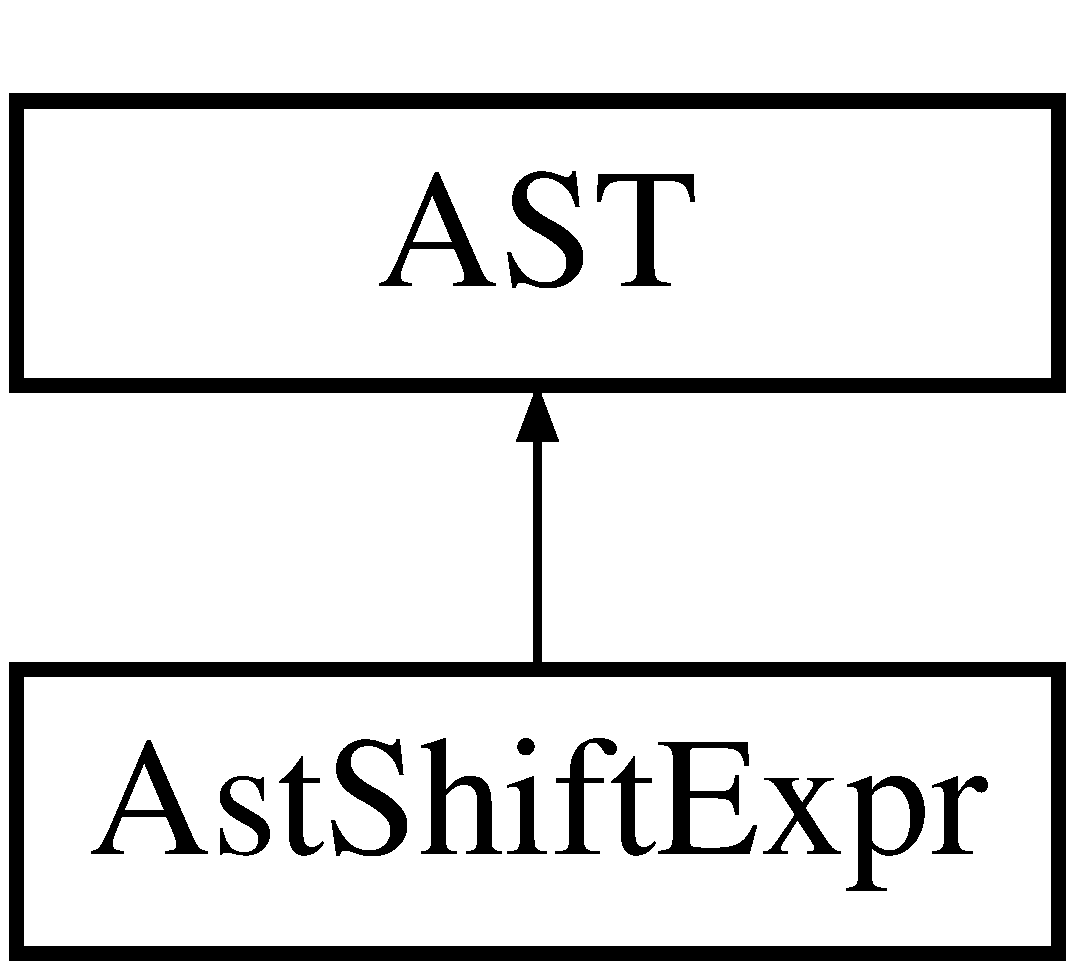
\includegraphics[height=2.000000cm]{classAstShiftExpr}
\end{center}
\end{figure}
\subsection*{Public Types}
\begin{DoxyCompactItemize}
\item 
enum {\bfseries Operator} \{ {\bfseries N\-O\-N\-E}, 
{\bfseries L\-E\-F\-T\-\_\-\-O\-P}, 
{\bfseries R\-I\-G\-H\-T\-\_\-\-O\-P}
 \}
\end{DoxyCompactItemize}
\subsection*{Public Member Functions}
\begin{DoxyCompactItemize}
\item 
\hypertarget{classAstShiftExpr_ae85c464914cce70d3ebb4f51b898781f}{{\bfseries Ast\-Shift\-Expr} (\hyperlink{classAstAddExpr}{Ast\-Add\-Expr} $\ast$a)}\label{classAstShiftExpr_ae85c464914cce70d3ebb4f51b898781f}

\item 
\hypertarget{classAstShiftExpr_a9c8c73a11d9e4da6264b1d83d4339cdb}{{\bfseries Ast\-Shift\-Expr} (\hyperlink{classAstShiftExpr}{Ast\-Shift\-Expr} $\ast$s, Operator o, \hyperlink{classAstAddExpr}{Ast\-Add\-Expr} $\ast$a)}\label{classAstShiftExpr_a9c8c73a11d9e4da6264b1d83d4339cdb}

\item 
void \hyperlink{classAstShiftExpr_ae20f0c9604ec1ca74911337e3ed375e5}{Visit} ()
\begin{DoxyCompactList}\small\item\em This function is responsible for tree traversals. \end{DoxyCompactList}\item 
void \hyperlink{classAST_a71d680856e95ff89f55d5311a552eba6}{set\-Label} (string l)
\begin{DoxyCompactList}\small\item\em Sets the label for the node. \end{DoxyCompactList}\item 
int \hyperlink{classAST_ab7a5b1d9f1c2de0d98deb356f724a42c}{get\-U\-I\-D} ()
\begin{DoxyCompactList}\small\item\em Gets the node's unique I\-D. \end{DoxyCompactList}\item 
string \hyperlink{classAST_aee029be902fffc927d16ccb03eb922ad}{get\-Label} ()
\begin{DoxyCompactList}\small\item\em Gets the node's label. \end{DoxyCompactList}\end{DoxyCompactItemize}
\subsection*{Public Attributes}
\begin{DoxyCompactItemize}
\item 
\hypertarget{classAstShiftExpr_a637fba35ffc19fe4da9569d92ab704ea}{enum Ast\-Shift\-Expr\-::\-Operator {\bfseries op}}\label{classAstShiftExpr_a637fba35ffc19fe4da9569d92ab704ea}

\end{DoxyCompactItemize}
\subsection*{Static Public Attributes}
\begin{DoxyCompactItemize}
\item 
\hypertarget{classAST_aca9e6637209b31e03a09c0d42f29bdfa}{static \hyperlink{classVisualizer}{Visualizer} \hyperlink{classAST_aca9e6637209b31e03a09c0d42f29bdfa}{vis}}\label{classAST_aca9e6637209b31e03a09c0d42f29bdfa}

\begin{DoxyCompactList}\small\item\em Static visualizer instance for generating the visualization of the \hyperlink{classAST}{A\-S\-T}. \end{DoxyCompactList}\end{DoxyCompactItemize}
\subsection*{Protected Attributes}
\begin{DoxyCompactItemize}
\item 
\hypertarget{classAST_a847b778f1c3dd5a19de32de432ee6e15}{int \hyperlink{classAST_a847b778f1c3dd5a19de32de432ee6e15}{uid}}\label{classAST_a847b778f1c3dd5a19de32de432ee6e15}

\begin{DoxyCompactList}\small\item\em The unique id. \end{DoxyCompactList}\item 
\hypertarget{classAST_ab2e239ccc0688d2341724432ff5a1a31}{string \hyperlink{classAST_ab2e239ccc0688d2341724432ff5a1a31}{label}}\label{classAST_ab2e239ccc0688d2341724432ff5a1a31}

\begin{DoxyCompactList}\small\item\em The label to be printed in the visualization. \end{DoxyCompactList}\end{DoxyCompactItemize}
\subsection*{Private Attributes}
\begin{DoxyCompactItemize}
\item 
\hypertarget{classAstShiftExpr_ab7f53d7e78fc19e580097130d2298aa2}{\hyperlink{classAstAddExpr}{Ast\-Add\-Expr} $\ast$ {\bfseries add}}\label{classAstShiftExpr_ab7f53d7e78fc19e580097130d2298aa2}

\item 
\hypertarget{classAstShiftExpr_a8609437ab341b8c26e2aa138d3cae348}{\hyperlink{classAstShiftExpr}{Ast\-Shift\-Expr} $\ast$ {\bfseries shift}}\label{classAstShiftExpr_a8609437ab341b8c26e2aa138d3cae348}

\end{DoxyCompactItemize}


\subsection{Member Function Documentation}
\hypertarget{classAST_aee029be902fffc927d16ccb03eb922ad}{\index{Ast\-Shift\-Expr@{Ast\-Shift\-Expr}!get\-Label@{get\-Label}}
\index{get\-Label@{get\-Label}!AstShiftExpr@{Ast\-Shift\-Expr}}
\subsubsection[{get\-Label}]{\setlength{\rightskip}{0pt plus 5cm}string A\-S\-T\-::get\-Label (
\begin{DoxyParamCaption}
{}
\end{DoxyParamCaption}
)\hspace{0.3cm}{\ttfamily [inline]}, {\ttfamily [inherited]}}}\label{classAST_aee029be902fffc927d16ccb03eb922ad}


Gets the node's label. 

\begin{DoxyReturn}{Returns}
The label 
\end{DoxyReturn}
\hypertarget{classAST_ab7a5b1d9f1c2de0d98deb356f724a42c}{\index{Ast\-Shift\-Expr@{Ast\-Shift\-Expr}!get\-U\-I\-D@{get\-U\-I\-D}}
\index{get\-U\-I\-D@{get\-U\-I\-D}!AstShiftExpr@{Ast\-Shift\-Expr}}
\subsubsection[{get\-U\-I\-D}]{\setlength{\rightskip}{0pt plus 5cm}int A\-S\-T\-::get\-U\-I\-D (
\begin{DoxyParamCaption}
{}
\end{DoxyParamCaption}
)\hspace{0.3cm}{\ttfamily [inline]}, {\ttfamily [inherited]}}}\label{classAST_ab7a5b1d9f1c2de0d98deb356f724a42c}


Gets the node's unique I\-D. 

\begin{DoxyReturn}{Returns}
The unique id 
\end{DoxyReturn}
\hypertarget{classAST_a71d680856e95ff89f55d5311a552eba6}{\index{Ast\-Shift\-Expr@{Ast\-Shift\-Expr}!set\-Label@{set\-Label}}
\index{set\-Label@{set\-Label}!AstShiftExpr@{Ast\-Shift\-Expr}}
\subsubsection[{set\-Label}]{\setlength{\rightskip}{0pt plus 5cm}void A\-S\-T\-::set\-Label (
\begin{DoxyParamCaption}
\item[{string}]{l}
\end{DoxyParamCaption}
)\hspace{0.3cm}{\ttfamily [inline]}, {\ttfamily [inherited]}}}\label{classAST_a71d680856e95ff89f55d5311a552eba6}


Sets the label for the node. 


\begin{DoxyParams}{Parameters}
{\em l} & The label string \\
\hline
\end{DoxyParams}
\hypertarget{classAstShiftExpr_ae20f0c9604ec1ca74911337e3ed375e5}{\index{Ast\-Shift\-Expr@{Ast\-Shift\-Expr}!Visit@{Visit}}
\index{Visit@{Visit}!AstShiftExpr@{Ast\-Shift\-Expr}}
\subsubsection[{Visit}]{\setlength{\rightskip}{0pt plus 5cm}void Ast\-Shift\-Expr\-::\-Visit (
\begin{DoxyParamCaption}
{}
\end{DoxyParamCaption}
)\hspace{0.3cm}{\ttfamily [virtual]}}}\label{classAstShiftExpr_ae20f0c9604ec1ca74911337e3ed375e5}


This function is responsible for tree traversals. 

This function will call the Visit functions of each of it's children nodes, call the visualization code for itself, and output any 3\-A\-C that can be generated at the current node. 

Reimplemented from \hyperlink{classAST_a5828cc86f2c4f1a0aeab6d7069e8fd82}{A\-S\-T}.



The documentation for this class was generated from the following files\-:\begin{DoxyCompactItemize}
\item 
Ast.\-h\item 
Ast.\-cpp\end{DoxyCompactItemize}

\input{classAstSpeciQualList}
\hypertarget{classAstStatement}{\section{Ast\-Statement Class Reference}
\label{classAstStatement}\index{Ast\-Statement@{Ast\-Statement}}
}
Inheritance diagram for Ast\-Statement\-:\begin{figure}[H]
\begin{center}
\leavevmode
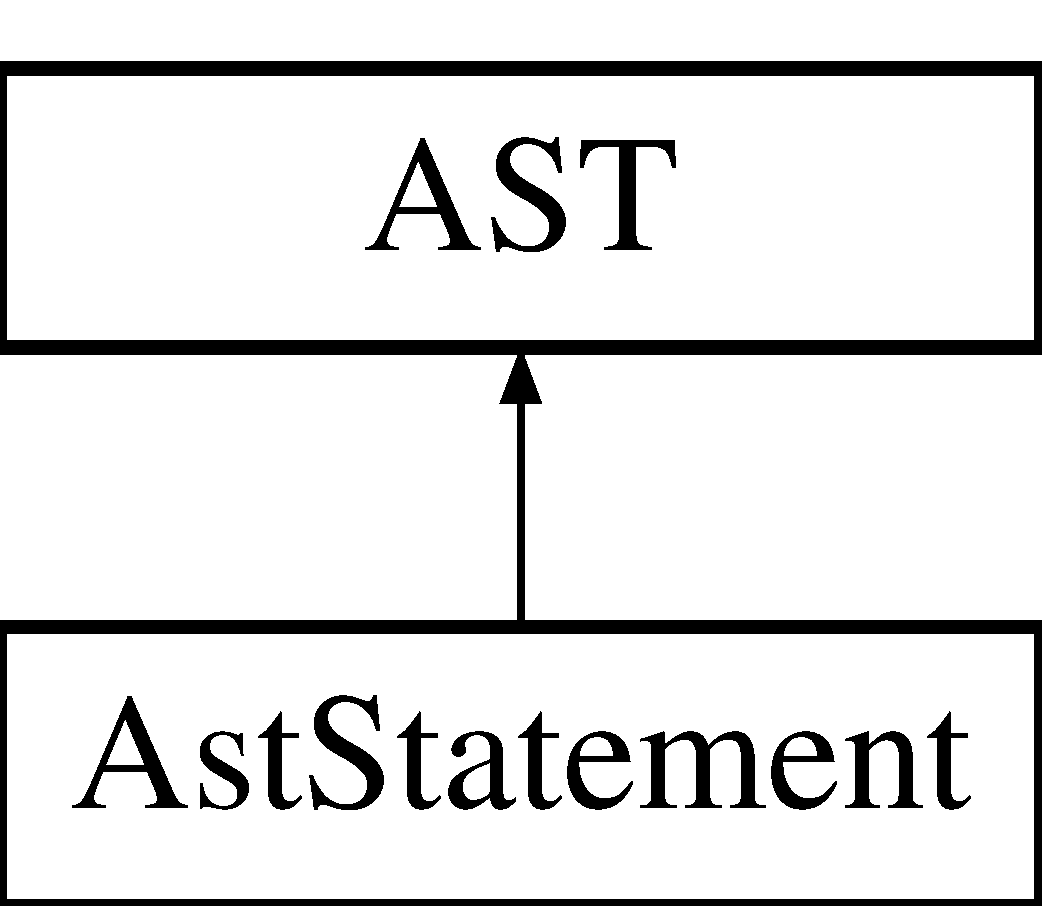
\includegraphics[height=2.000000cm]{classAstStatement}
\end{center}
\end{figure}
\subsection*{Public Types}
\begin{DoxyCompactItemize}
\item 
enum {\bfseries Type} \{ \\*
{\bfseries L\-A\-B\-E\-L\-E\-D}, 
{\bfseries C\-O\-M\-P\-O\-U\-N\-D}, 
{\bfseries E\-X\-P\-R}, 
{\bfseries S\-E\-L\-E\-C\-T}, 
\\*
{\bfseries I\-T\-E\-R}, 
{\bfseries J\-U\-M\-P}, 
{\bfseries L\-A\-B\-E\-L\-E\-D}, 
{\bfseries C\-O\-M\-P\-O\-U\-N\-D}, 
\\*
{\bfseries E\-X\-P\-R}, 
{\bfseries S\-E\-L\-E\-C\-T}, 
{\bfseries I\-T\-E\-R}, 
{\bfseries J\-U\-M\-P}, 
\\*
{\bfseries L\-A\-B\-E\-L\-E\-D}, 
{\bfseries C\-O\-M\-P\-O\-U\-N\-D}, 
{\bfseries E\-X\-P\-R}, 
{\bfseries S\-E\-L\-E\-C\-T}, 
\\*
{\bfseries I\-T\-E\-R}, 
{\bfseries J\-U\-M\-P}, 
{\bfseries L\-A\-B\-E\-L\-E\-D}, 
{\bfseries C\-O\-M\-P\-O\-U\-N\-D}, 
\\*
{\bfseries E\-X\-P\-R}, 
{\bfseries S\-E\-L\-E\-C\-T}, 
{\bfseries I\-T\-E\-R}, 
{\bfseries J\-U\-M\-P}
 \}
\item 
enum {\bfseries Type} \{ \\*
{\bfseries L\-A\-B\-E\-L\-E\-D}, 
{\bfseries C\-O\-M\-P\-O\-U\-N\-D}, 
{\bfseries E\-X\-P\-R}, 
{\bfseries S\-E\-L\-E\-C\-T}, 
\\*
{\bfseries I\-T\-E\-R}, 
{\bfseries J\-U\-M\-P}, 
{\bfseries L\-A\-B\-E\-L\-E\-D}, 
{\bfseries C\-O\-M\-P\-O\-U\-N\-D}, 
\\*
{\bfseries E\-X\-P\-R}, 
{\bfseries S\-E\-L\-E\-C\-T}, 
{\bfseries I\-T\-E\-R}, 
{\bfseries J\-U\-M\-P}, 
\\*
{\bfseries L\-A\-B\-E\-L\-E\-D}, 
{\bfseries C\-O\-M\-P\-O\-U\-N\-D}, 
{\bfseries E\-X\-P\-R}, 
{\bfseries S\-E\-L\-E\-C\-T}, 
\\*
{\bfseries I\-T\-E\-R}, 
{\bfseries J\-U\-M\-P}, 
{\bfseries L\-A\-B\-E\-L\-E\-D}, 
{\bfseries C\-O\-M\-P\-O\-U\-N\-D}, 
\\*
{\bfseries E\-X\-P\-R}, 
{\bfseries S\-E\-L\-E\-C\-T}, 
{\bfseries I\-T\-E\-R}, 
{\bfseries J\-U\-M\-P}
 \}
\item 
enum {\bfseries Type} \{ \\*
{\bfseries L\-A\-B\-E\-L\-E\-D}, 
{\bfseries C\-O\-M\-P\-O\-U\-N\-D}, 
{\bfseries E\-X\-P\-R}, 
{\bfseries S\-E\-L\-E\-C\-T}, 
\\*
{\bfseries I\-T\-E\-R}, 
{\bfseries J\-U\-M\-P}, 
{\bfseries L\-A\-B\-E\-L\-E\-D}, 
{\bfseries C\-O\-M\-P\-O\-U\-N\-D}, 
\\*
{\bfseries E\-X\-P\-R}, 
{\bfseries S\-E\-L\-E\-C\-T}, 
{\bfseries I\-T\-E\-R}, 
{\bfseries J\-U\-M\-P}, 
\\*
{\bfseries L\-A\-B\-E\-L\-E\-D}, 
{\bfseries C\-O\-M\-P\-O\-U\-N\-D}, 
{\bfseries E\-X\-P\-R}, 
{\bfseries S\-E\-L\-E\-C\-T}, 
\\*
{\bfseries I\-T\-E\-R}, 
{\bfseries J\-U\-M\-P}, 
{\bfseries L\-A\-B\-E\-L\-E\-D}, 
{\bfseries C\-O\-M\-P\-O\-U\-N\-D}, 
\\*
{\bfseries E\-X\-P\-R}, 
{\bfseries S\-E\-L\-E\-C\-T}, 
{\bfseries I\-T\-E\-R}, 
{\bfseries J\-U\-M\-P}
 \}
\item 
enum {\bfseries Type} \{ \\*
{\bfseries L\-A\-B\-E\-L\-E\-D}, 
{\bfseries C\-O\-M\-P\-O\-U\-N\-D}, 
{\bfseries E\-X\-P\-R}, 
{\bfseries S\-E\-L\-E\-C\-T}, 
\\*
{\bfseries I\-T\-E\-R}, 
{\bfseries J\-U\-M\-P}, 
{\bfseries L\-A\-B\-E\-L\-E\-D}, 
{\bfseries C\-O\-M\-P\-O\-U\-N\-D}, 
\\*
{\bfseries E\-X\-P\-R}, 
{\bfseries S\-E\-L\-E\-C\-T}, 
{\bfseries I\-T\-E\-R}, 
{\bfseries J\-U\-M\-P}, 
\\*
{\bfseries L\-A\-B\-E\-L\-E\-D}, 
{\bfseries C\-O\-M\-P\-O\-U\-N\-D}, 
{\bfseries E\-X\-P\-R}, 
{\bfseries S\-E\-L\-E\-C\-T}, 
\\*
{\bfseries I\-T\-E\-R}, 
{\bfseries J\-U\-M\-P}, 
{\bfseries L\-A\-B\-E\-L\-E\-D}, 
{\bfseries C\-O\-M\-P\-O\-U\-N\-D}, 
\\*
{\bfseries E\-X\-P\-R}, 
{\bfseries S\-E\-L\-E\-C\-T}, 
{\bfseries I\-T\-E\-R}, 
{\bfseries J\-U\-M\-P}
 \}
\end{DoxyCompactItemize}
\subsection*{Public Member Functions}
\begin{DoxyCompactItemize}
\item 
\hypertarget{classAstStatement_a51c4738b3eb4d0ce7f7937580827df49}{{\bfseries Ast\-Statement} (\hyperlink{classAstLabeledStmt}{Ast\-Labeled\-Stmt} $\ast$l)}\label{classAstStatement_a51c4738b3eb4d0ce7f7937580827df49}

\item 
\hypertarget{classAstStatement_a06ab5906e58059421ffca709140ad1b0}{{\bfseries Ast\-Statement} (\hyperlink{classAstCompoundStmt}{Ast\-Compound\-Stmt} $\ast$c)}\label{classAstStatement_a06ab5906e58059421ffca709140ad1b0}

\item 
\hypertarget{classAstStatement_a8a44969c79b381d9cef932fc93d99339}{{\bfseries Ast\-Statement} (\hyperlink{classAstExprStmt}{Ast\-Expr\-Stmt} $\ast$e)}\label{classAstStatement_a8a44969c79b381d9cef932fc93d99339}

\item 
\hypertarget{classAstStatement_a8bc036f0b37cacbfa99159e4c57207ec}{{\bfseries Ast\-Statement} (\hyperlink{classAstSelection}{Ast\-Selection} $\ast$s)}\label{classAstStatement_a8bc036f0b37cacbfa99159e4c57207ec}

\item 
\hypertarget{classAstStatement_ae26acf207adc2d426e558e5889b43b54}{{\bfseries Ast\-Statement} (\hyperlink{classAstIteration}{Ast\-Iteration} $\ast$i)}\label{classAstStatement_ae26acf207adc2d426e558e5889b43b54}

\item 
\hypertarget{classAstStatement_a80c754bbc909f7e2e7938e90485d7065}{{\bfseries Ast\-Statement} (\hyperlink{classAstJump}{Ast\-Jump} $\ast$j)}\label{classAstStatement_a80c754bbc909f7e2e7938e90485d7065}

\item 
void \hyperlink{classAstStatement_a1f1570931e373fe2f1e18ce417236ee4}{Visit} ()
\begin{DoxyCompactList}\small\item\em This function is responsible for tree traversals. \end{DoxyCompactList}\item 
\hypertarget{classAstStatement_a51c4738b3eb4d0ce7f7937580827df49}{{\bfseries Ast\-Statement} (\hyperlink{classAstLabeledStmt}{Ast\-Labeled\-Stmt} $\ast$l)}\label{classAstStatement_a51c4738b3eb4d0ce7f7937580827df49}

\item 
\hypertarget{classAstStatement_a06ab5906e58059421ffca709140ad1b0}{{\bfseries Ast\-Statement} (\hyperlink{classAstCompoundStmt}{Ast\-Compound\-Stmt} $\ast$c)}\label{classAstStatement_a06ab5906e58059421ffca709140ad1b0}

\item 
\hypertarget{classAstStatement_a8a44969c79b381d9cef932fc93d99339}{{\bfseries Ast\-Statement} (\hyperlink{classAstExprStmt}{Ast\-Expr\-Stmt} $\ast$e)}\label{classAstStatement_a8a44969c79b381d9cef932fc93d99339}

\item 
\hypertarget{classAstStatement_a8bc036f0b37cacbfa99159e4c57207ec}{{\bfseries Ast\-Statement} (\hyperlink{classAstSelection}{Ast\-Selection} $\ast$s)}\label{classAstStatement_a8bc036f0b37cacbfa99159e4c57207ec}

\item 
\hypertarget{classAstStatement_ae26acf207adc2d426e558e5889b43b54}{{\bfseries Ast\-Statement} (\hyperlink{classAstIteration}{Ast\-Iteration} $\ast$i)}\label{classAstStatement_ae26acf207adc2d426e558e5889b43b54}

\item 
\hypertarget{classAstStatement_a80c754bbc909f7e2e7938e90485d7065}{{\bfseries Ast\-Statement} (\hyperlink{classAstJump}{Ast\-Jump} $\ast$j)}\label{classAstStatement_a80c754bbc909f7e2e7938e90485d7065}

\item 
void \hyperlink{classAstStatement_a1f1570931e373fe2f1e18ce417236ee4}{Visit} ()
\begin{DoxyCompactList}\small\item\em This function is responsible for tree traversals. \end{DoxyCompactList}\item 
\hypertarget{classAstStatement_a51c4738b3eb4d0ce7f7937580827df49}{{\bfseries Ast\-Statement} (\hyperlink{classAstLabeledStmt}{Ast\-Labeled\-Stmt} $\ast$l)}\label{classAstStatement_a51c4738b3eb4d0ce7f7937580827df49}

\item 
\hypertarget{classAstStatement_a06ab5906e58059421ffca709140ad1b0}{{\bfseries Ast\-Statement} (\hyperlink{classAstCompoundStmt}{Ast\-Compound\-Stmt} $\ast$c)}\label{classAstStatement_a06ab5906e58059421ffca709140ad1b0}

\item 
\hypertarget{classAstStatement_a8a44969c79b381d9cef932fc93d99339}{{\bfseries Ast\-Statement} (\hyperlink{classAstExprStmt}{Ast\-Expr\-Stmt} $\ast$e)}\label{classAstStatement_a8a44969c79b381d9cef932fc93d99339}

\item 
\hypertarget{classAstStatement_a8bc036f0b37cacbfa99159e4c57207ec}{{\bfseries Ast\-Statement} (\hyperlink{classAstSelection}{Ast\-Selection} $\ast$s)}\label{classAstStatement_a8bc036f0b37cacbfa99159e4c57207ec}

\item 
\hypertarget{classAstStatement_ae26acf207adc2d426e558e5889b43b54}{{\bfseries Ast\-Statement} (\hyperlink{classAstIteration}{Ast\-Iteration} $\ast$i)}\label{classAstStatement_ae26acf207adc2d426e558e5889b43b54}

\item 
\hypertarget{classAstStatement_a80c754bbc909f7e2e7938e90485d7065}{{\bfseries Ast\-Statement} (\hyperlink{classAstJump}{Ast\-Jump} $\ast$j)}\label{classAstStatement_a80c754bbc909f7e2e7938e90485d7065}

\item 
void \hyperlink{classAstStatement_a1f1570931e373fe2f1e18ce417236ee4}{Visit} ()
\begin{DoxyCompactList}\small\item\em This function is responsible for tree traversals. \end{DoxyCompactList}\item 
\hypertarget{classAstStatement_a51c4738b3eb4d0ce7f7937580827df49}{{\bfseries Ast\-Statement} (\hyperlink{classAstLabeledStmt}{Ast\-Labeled\-Stmt} $\ast$l)}\label{classAstStatement_a51c4738b3eb4d0ce7f7937580827df49}

\item 
\hypertarget{classAstStatement_a06ab5906e58059421ffca709140ad1b0}{{\bfseries Ast\-Statement} (\hyperlink{classAstCompoundStmt}{Ast\-Compound\-Stmt} $\ast$c)}\label{classAstStatement_a06ab5906e58059421ffca709140ad1b0}

\item 
\hypertarget{classAstStatement_a8a44969c79b381d9cef932fc93d99339}{{\bfseries Ast\-Statement} (\hyperlink{classAstExprStmt}{Ast\-Expr\-Stmt} $\ast$e)}\label{classAstStatement_a8a44969c79b381d9cef932fc93d99339}

\item 
\hypertarget{classAstStatement_a8bc036f0b37cacbfa99159e4c57207ec}{{\bfseries Ast\-Statement} (\hyperlink{classAstSelection}{Ast\-Selection} $\ast$s)}\label{classAstStatement_a8bc036f0b37cacbfa99159e4c57207ec}

\item 
\hypertarget{classAstStatement_ae26acf207adc2d426e558e5889b43b54}{{\bfseries Ast\-Statement} (\hyperlink{classAstIteration}{Ast\-Iteration} $\ast$i)}\label{classAstStatement_ae26acf207adc2d426e558e5889b43b54}

\item 
\hypertarget{classAstStatement_a80c754bbc909f7e2e7938e90485d7065}{{\bfseries Ast\-Statement} (\hyperlink{classAstJump}{Ast\-Jump} $\ast$j)}\label{classAstStatement_a80c754bbc909f7e2e7938e90485d7065}

\item 
void \hyperlink{classAstStatement_a1f1570931e373fe2f1e18ce417236ee4}{Visit} ()
\begin{DoxyCompactList}\small\item\em This function is responsible for tree traversals. \end{DoxyCompactList}\item 
void \hyperlink{classAST_a71d680856e95ff89f55d5311a552eba6}{set\-Label} (string l)
\begin{DoxyCompactList}\small\item\em Sets the label for the node. \end{DoxyCompactList}\item 
void \hyperlink{classAST_a71d680856e95ff89f55d5311a552eba6}{set\-Label} (string l)
\begin{DoxyCompactList}\small\item\em Sets the label for the node. \end{DoxyCompactList}\item 
void \hyperlink{classAST_a71d680856e95ff89f55d5311a552eba6}{set\-Label} (string l)
\begin{DoxyCompactList}\small\item\em Sets the label for the node. \end{DoxyCompactList}\item 
void \hyperlink{classAST_a71d680856e95ff89f55d5311a552eba6}{set\-Label} (string l)
\begin{DoxyCompactList}\small\item\em Sets the label for the node. \end{DoxyCompactList}\item 
int \hyperlink{classAST_ab7a5b1d9f1c2de0d98deb356f724a42c}{get\-U\-I\-D} ()
\begin{DoxyCompactList}\small\item\em Gets the node's unique I\-D. \end{DoxyCompactList}\item 
int \hyperlink{classAST_ab7a5b1d9f1c2de0d98deb356f724a42c}{get\-U\-I\-D} ()
\begin{DoxyCompactList}\small\item\em Gets the node's unique I\-D. \end{DoxyCompactList}\item 
int \hyperlink{classAST_ab7a5b1d9f1c2de0d98deb356f724a42c}{get\-U\-I\-D} ()
\begin{DoxyCompactList}\small\item\em Gets the node's unique I\-D. \end{DoxyCompactList}\item 
int \hyperlink{classAST_ab7a5b1d9f1c2de0d98deb356f724a42c}{get\-U\-I\-D} ()
\begin{DoxyCompactList}\small\item\em Gets the node's unique I\-D. \end{DoxyCompactList}\item 
string \hyperlink{classAST_aee029be902fffc927d16ccb03eb922ad}{get\-Label} ()
\begin{DoxyCompactList}\small\item\em Gets the node's label. \end{DoxyCompactList}\item 
string \hyperlink{classAST_aee029be902fffc927d16ccb03eb922ad}{get\-Label} ()
\begin{DoxyCompactList}\small\item\em Gets the node's label. \end{DoxyCompactList}\item 
string \hyperlink{classAST_aee029be902fffc927d16ccb03eb922ad}{get\-Label} ()
\begin{DoxyCompactList}\small\item\em Gets the node's label. \end{DoxyCompactList}\item 
string \hyperlink{classAST_aee029be902fffc927d16ccb03eb922ad}{get\-Label} ()
\begin{DoxyCompactList}\small\item\em Gets the node's label. \end{DoxyCompactList}\end{DoxyCompactItemize}
\subsection*{Public Attributes}
\begin{DoxyCompactItemize}
\item 
\hypertarget{classAstStatement_a79670f71bfdd5ba5c3c386c3b5f8e5dd}{enum Ast\-Statement\-::\-Type {\bfseries t}}\label{classAstStatement_a79670f71bfdd5ba5c3c386c3b5f8e5dd}

\item 
\hypertarget{classAST_aaf215802de409f8096c063d01ffa6783}{bool \hyperlink{classAST_aaf215802de409f8096c063d01ffa6783}{needs\-Cast}}\label{classAST_aaf215802de409f8096c063d01ffa6783}

\begin{DoxyCompactList}\small\item\em This indicates if cast 3\-A\-C needs to be output, and is only relevant for expressions. \end{DoxyCompactList}\item 
\hypertarget{classAST_afa9e77ef650ec6664458fa6cb55be985}{bool \hyperlink{classAST_afa9e77ef650ec6664458fa6cb55be985}{is\-Conv}}\label{classAST_afa9e77ef650ec6664458fa6cb55be985}

\begin{DoxyCompactList}\small\item\em Indicates is a conversion is possible. \end{DoxyCompactList}\item 
\hypertarget{classAST_a61ef3317e023d45237e06615b387cd6b}{C\-O\-N\-V\-E\-R\-S\-I\-O\-N\-T\-Y\-P\-E \hyperlink{classAST_a61ef3317e023d45237e06615b387cd6b}{conv\-Type}}\label{classAST_a61ef3317e023d45237e06615b387cd6b}

\begin{DoxyCompactList}\small\item\em If needs\-Cast is true, then this indicates what the cast should be. \end{DoxyCompactList}\item 
\hypertarget{classAST_aea9b07b39d24183f38c0029cec0a878e}{int \hyperlink{classAST_aea9b07b39d24183f38c0029cec0a878e}{operand\-To\-Cast}}\label{classAST_aea9b07b39d24183f38c0029cec0a878e}

\begin{DoxyCompactList}\small\item\em This indicates if the first or second operand should be the one that is cast. \end{DoxyCompactList}\end{DoxyCompactItemize}
\subsection*{Static Public Attributes}
\begin{DoxyCompactItemize}
\item 
\hypertarget{classAST_a5fdfd5f7b104dd92889163bdadbc68d6}{static \hyperlink{classVisualizer}{Visualizer} \hyperlink{classAST_a5fdfd5f7b104dd92889163bdadbc68d6}{vis}}\label{classAST_a5fdfd5f7b104dd92889163bdadbc68d6}

\begin{DoxyCompactList}\small\item\em Static visualizer instance for generating the visualization of the \hyperlink{classAST}{A\-S\-T}. \end{DoxyCompactList}\item 
\hypertarget{classAST_a8a3ace322f50e030331065d644ee55ee}{static \hyperlink{classTAC__Generator}{T\-A\-C\-\_\-\-Generator} \hyperlink{classAST_a8a3ace322f50e030331065d644ee55ee}{tac\-Gen}}\label{classAST_a8a3ace322f50e030331065d644ee55ee}

\begin{DoxyCompactList}\small\item\em Three address code generator. \end{DoxyCompactList}\item 
\hypertarget{classAST_a1f69448c6dc368d005631a128460083d}{static string {\bfseries current\-Temp} =\char`\"{}\char`\"{}}\label{classAST_a1f69448c6dc368d005631a128460083d}

\item 
\hypertarget{classAST_a551aec090c932ab69365238b40a8a4eb}{static string \hyperlink{classAST_a551aec090c932ab69365238b40a8a4eb}{return\-Label} =\char`\"{}\char`\"{}}\label{classAST_a551aec090c932ab69365238b40a8a4eb}

\begin{DoxyCompactList}\small\item\em This is for storing the string id of any temporary result register that may be created during 3\-A\-C generation. \end{DoxyCompactList}\item 
\hypertarget{classAST_a73c0a266df52be71e6b527b6aa635173}{static list$<$ string $>$ {\bfseries temp\-Stack}}\label{classAST_a73c0a266df52be71e6b527b6aa635173}

\item 
\hypertarget{classAST_abf9e84b541ff04b7bb64e6e4371512d4}{static string {\bfseries last\-I\-D} =\char`\"{}\char`\"{}}\label{classAST_abf9e84b541ff04b7bb64e6e4371512d4}

\item 
\hypertarget{classAST_a163003bfe9c30510ec8039870346049f}{static \hyperlink{classSymTab}{Sym\-Tab} $\ast$ {\bfseries symbol\-Table} =N\-U\-L\-L}\label{classAST_a163003bfe9c30510ec8039870346049f}

\item 
\hypertarget{classAST_a5c3cc894d9c0453523dec9ed76f18a04}{static string {\bfseries current\-Function} =\char`\"{}\char`\"{}}\label{classAST_a5c3cc894d9c0453523dec9ed76f18a04}

\item 
\hypertarget{classAST_a66155513b59ff1a04c8ece8b20ec31f5}{static int {\bfseries current\-Constant\-Value} =0}\label{classAST_a66155513b59ff1a04c8ece8b20ec31f5}

\item 
\hypertarget{classAST_a3d031d7bab635ba1f015aade5943f40c}{static string {\bfseries current\-Id\-Name} =\char`\"{}\char`\"{}}\label{classAST_a3d031d7bab635ba1f015aade5943f40c}

\item 
\hypertarget{classAST_a16c4b6e54febc1a26b31a64a46972ef0}{static int {\bfseries current\-Index\-Val} = 0}\label{classAST_a16c4b6e54febc1a26b31a64a46972ef0}

\item 
\hypertarget{classAST_a6fc65ae9dd064a88941d4b88669b19db}{static string {\bfseries current\-I\-D} = \char`\"{}\char`\"{}}\label{classAST_a6fc65ae9dd064a88941d4b88669b19db}

\end{DoxyCompactItemize}
\subsection*{Protected Attributes}
\begin{DoxyCompactItemize}
\item 
\hypertarget{classAST_a847b778f1c3dd5a19de32de432ee6e15}{int \hyperlink{classAST_a847b778f1c3dd5a19de32de432ee6e15}{uid}}\label{classAST_a847b778f1c3dd5a19de32de432ee6e15}

\begin{DoxyCompactList}\small\item\em The unique id. \end{DoxyCompactList}\item 
\hypertarget{classAST_ab2e239ccc0688d2341724432ff5a1a31}{string \hyperlink{classAST_ab2e239ccc0688d2341724432ff5a1a31}{label}}\label{classAST_ab2e239ccc0688d2341724432ff5a1a31}

\begin{DoxyCompactList}\small\item\em The label to be printed in the visualization. \end{DoxyCompactList}\end{DoxyCompactItemize}
\subsection*{Private Attributes}
\begin{DoxyCompactItemize}
\item 
\hypertarget{classAstStatement_a959cdc8445704afd0743323ff1187864}{\hyperlink{classAstLabeledStmt}{Ast\-Labeled\-Stmt} $\ast$ {\bfseries lbl}}\label{classAstStatement_a959cdc8445704afd0743323ff1187864}

\item 
\hypertarget{classAstStatement_abe55f8a5598959cbfc98905a3c7f3c61}{\hyperlink{classAstCompoundStmt}{Ast\-Compound\-Stmt} $\ast$ {\bfseries cmp}}\label{classAstStatement_abe55f8a5598959cbfc98905a3c7f3c61}

\item 
\hypertarget{classAstStatement_a233bc02d0b2ea3cceae7b483644a7be8}{\hyperlink{classAstExprStmt}{Ast\-Expr\-Stmt} $\ast$ {\bfseries expr}}\label{classAstStatement_a233bc02d0b2ea3cceae7b483644a7be8}

\item 
\hypertarget{classAstStatement_a38f48fb1951a4e4aef699e20d620220d}{\hyperlink{classAstSelection}{Ast\-Selection} $\ast$ {\bfseries slct}}\label{classAstStatement_a38f48fb1951a4e4aef699e20d620220d}

\item 
\hypertarget{classAstStatement_a7a48aafdfcb5e6d36608d0c751a146bf}{\hyperlink{classAstIteration}{Ast\-Iteration} $\ast$ {\bfseries iter}}\label{classAstStatement_a7a48aafdfcb5e6d36608d0c751a146bf}

\item 
\hypertarget{classAstStatement_adce7399aacd5d715c3c527de0caf78bf}{\hyperlink{classAstJump}{Ast\-Jump} $\ast$ {\bfseries jump}}\label{classAstStatement_adce7399aacd5d715c3c527de0caf78bf}

\end{DoxyCompactItemize}


\subsection{Detailed Description}


Definition at line 987 of file Ast.\-h.



\subsection{Member Function Documentation}
\hypertarget{classAST_aee029be902fffc927d16ccb03eb922ad}{\index{Ast\-Statement@{Ast\-Statement}!get\-Label@{get\-Label}}
\index{get\-Label@{get\-Label}!AstStatement@{Ast\-Statement}}
\subsubsection[{get\-Label}]{\setlength{\rightskip}{0pt plus 5cm}string A\-S\-T\-::get\-Label (
\begin{DoxyParamCaption}
{}
\end{DoxyParamCaption}
)\hspace{0.3cm}{\ttfamily [inline]}, {\ttfamily [inherited]}}}\label{classAST_aee029be902fffc927d16ccb03eb922ad}


Gets the node's label. 

\begin{DoxyReturn}{Returns}
The label 
\end{DoxyReturn}


Definition at line 60 of file Ast.\-h.

\hypertarget{classAST_aee029be902fffc927d16ccb03eb922ad}{\index{Ast\-Statement@{Ast\-Statement}!get\-Label@{get\-Label}}
\index{get\-Label@{get\-Label}!AstStatement@{Ast\-Statement}}
\subsubsection[{get\-Label}]{\setlength{\rightskip}{0pt plus 5cm}string A\-S\-T\-::get\-Label (
\begin{DoxyParamCaption}
{}
\end{DoxyParamCaption}
)\hspace{0.3cm}{\ttfamily [inline]}, {\ttfamily [inherited]}}}\label{classAST_aee029be902fffc927d16ccb03eb922ad}


Gets the node's label. 

\begin{DoxyReturn}{Returns}
The label 
\end{DoxyReturn}


Definition at line 60 of file C\-Scanner.\-ll.

\hypertarget{classAST_aee029be902fffc927d16ccb03eb922ad}{\index{Ast\-Statement@{Ast\-Statement}!get\-Label@{get\-Label}}
\index{get\-Label@{get\-Label}!AstStatement@{Ast\-Statement}}
\subsubsection[{get\-Label}]{\setlength{\rightskip}{0pt plus 5cm}string A\-S\-T\-::get\-Label (
\begin{DoxyParamCaption}
{}
\end{DoxyParamCaption}
)\hspace{0.3cm}{\ttfamily [inline]}, {\ttfamily [inherited]}}}\label{classAST_aee029be902fffc927d16ccb03eb922ad}


Gets the node's label. 

\begin{DoxyReturn}{Returns}
The label 
\end{DoxyReturn}


Definition at line 60 of file C\-Parser.\-yy.

\hypertarget{classAST_aee029be902fffc927d16ccb03eb922ad}{\index{Ast\-Statement@{Ast\-Statement}!get\-Label@{get\-Label}}
\index{get\-Label@{get\-Label}!AstStatement@{Ast\-Statement}}
\subsubsection[{get\-Label}]{\setlength{\rightskip}{0pt plus 5cm}string A\-S\-T\-::get\-Label (
\begin{DoxyParamCaption}
{}
\end{DoxyParamCaption}
)\hspace{0.3cm}{\ttfamily [inline]}, {\ttfamily [inherited]}}}\label{classAST_aee029be902fffc927d16ccb03eb922ad}


Gets the node's label. 

\begin{DoxyReturn}{Returns}
The label 
\end{DoxyReturn}


Definition at line 60 of file C\-Parser.\-yy.

\hypertarget{classAST_ab7a5b1d9f1c2de0d98deb356f724a42c}{\index{Ast\-Statement@{Ast\-Statement}!get\-U\-I\-D@{get\-U\-I\-D}}
\index{get\-U\-I\-D@{get\-U\-I\-D}!AstStatement@{Ast\-Statement}}
\subsubsection[{get\-U\-I\-D}]{\setlength{\rightskip}{0pt plus 5cm}int A\-S\-T\-::get\-U\-I\-D (
\begin{DoxyParamCaption}
{}
\end{DoxyParamCaption}
)\hspace{0.3cm}{\ttfamily [inline]}, {\ttfamily [inherited]}}}\label{classAST_ab7a5b1d9f1c2de0d98deb356f724a42c}


Gets the node's unique I\-D. 

\begin{DoxyReturn}{Returns}
The unique id 
\end{DoxyReturn}


Definition at line 53 of file C\-Parser.\-yy.

\hypertarget{classAST_ab7a5b1d9f1c2de0d98deb356f724a42c}{\index{Ast\-Statement@{Ast\-Statement}!get\-U\-I\-D@{get\-U\-I\-D}}
\index{get\-U\-I\-D@{get\-U\-I\-D}!AstStatement@{Ast\-Statement}}
\subsubsection[{get\-U\-I\-D}]{\setlength{\rightskip}{0pt plus 5cm}int A\-S\-T\-::get\-U\-I\-D (
\begin{DoxyParamCaption}
{}
\end{DoxyParamCaption}
)\hspace{0.3cm}{\ttfamily [inline]}, {\ttfamily [inherited]}}}\label{classAST_ab7a5b1d9f1c2de0d98deb356f724a42c}


Gets the node's unique I\-D. 

\begin{DoxyReturn}{Returns}
The unique id 
\end{DoxyReturn}


Definition at line 53 of file C\-Parser.\-yy.

\hypertarget{classAST_ab7a5b1d9f1c2de0d98deb356f724a42c}{\index{Ast\-Statement@{Ast\-Statement}!get\-U\-I\-D@{get\-U\-I\-D}}
\index{get\-U\-I\-D@{get\-U\-I\-D}!AstStatement@{Ast\-Statement}}
\subsubsection[{get\-U\-I\-D}]{\setlength{\rightskip}{0pt plus 5cm}int A\-S\-T\-::get\-U\-I\-D (
\begin{DoxyParamCaption}
{}
\end{DoxyParamCaption}
)\hspace{0.3cm}{\ttfamily [inline]}, {\ttfamily [inherited]}}}\label{classAST_ab7a5b1d9f1c2de0d98deb356f724a42c}


Gets the node's unique I\-D. 

\begin{DoxyReturn}{Returns}
The unique id 
\end{DoxyReturn}


Definition at line 53 of file C\-Scanner.\-ll.

\hypertarget{classAST_ab7a5b1d9f1c2de0d98deb356f724a42c}{\index{Ast\-Statement@{Ast\-Statement}!get\-U\-I\-D@{get\-U\-I\-D}}
\index{get\-U\-I\-D@{get\-U\-I\-D}!AstStatement@{Ast\-Statement}}
\subsubsection[{get\-U\-I\-D}]{\setlength{\rightskip}{0pt plus 5cm}int A\-S\-T\-::get\-U\-I\-D (
\begin{DoxyParamCaption}
{}
\end{DoxyParamCaption}
)\hspace{0.3cm}{\ttfamily [inline]}, {\ttfamily [inherited]}}}\label{classAST_ab7a5b1d9f1c2de0d98deb356f724a42c}


Gets the node's unique I\-D. 

\begin{DoxyReturn}{Returns}
The unique id 
\end{DoxyReturn}


Definition at line 53 of file Ast.\-h.

\hypertarget{classAST_a71d680856e95ff89f55d5311a552eba6}{\index{Ast\-Statement@{Ast\-Statement}!set\-Label@{set\-Label}}
\index{set\-Label@{set\-Label}!AstStatement@{Ast\-Statement}}
\subsubsection[{set\-Label}]{\setlength{\rightskip}{0pt plus 5cm}void A\-S\-T\-::set\-Label (
\begin{DoxyParamCaption}
\item[{string}]{l}
\end{DoxyParamCaption}
)\hspace{0.3cm}{\ttfamily [inline]}, {\ttfamily [inherited]}}}\label{classAST_a71d680856e95ff89f55d5311a552eba6}


Sets the label for the node. 


\begin{DoxyParams}{Parameters}
{\em l} & The label string \\
\hline
\end{DoxyParams}


Definition at line 43 of file C\-Scanner.\-ll.

\hypertarget{classAST_a71d680856e95ff89f55d5311a552eba6}{\index{Ast\-Statement@{Ast\-Statement}!set\-Label@{set\-Label}}
\index{set\-Label@{set\-Label}!AstStatement@{Ast\-Statement}}
\subsubsection[{set\-Label}]{\setlength{\rightskip}{0pt plus 5cm}void A\-S\-T\-::set\-Label (
\begin{DoxyParamCaption}
\item[{string}]{l}
\end{DoxyParamCaption}
)\hspace{0.3cm}{\ttfamily [inline]}, {\ttfamily [inherited]}}}\label{classAST_a71d680856e95ff89f55d5311a552eba6}


Sets the label for the node. 


\begin{DoxyParams}{Parameters}
{\em l} & The label string \\
\hline
\end{DoxyParams}


Definition at line 43 of file C\-Parser.\-yy.

\hypertarget{classAST_a71d680856e95ff89f55d5311a552eba6}{\index{Ast\-Statement@{Ast\-Statement}!set\-Label@{set\-Label}}
\index{set\-Label@{set\-Label}!AstStatement@{Ast\-Statement}}
\subsubsection[{set\-Label}]{\setlength{\rightskip}{0pt plus 5cm}void A\-S\-T\-::set\-Label (
\begin{DoxyParamCaption}
\item[{string}]{l}
\end{DoxyParamCaption}
)\hspace{0.3cm}{\ttfamily [inline]}, {\ttfamily [inherited]}}}\label{classAST_a71d680856e95ff89f55d5311a552eba6}


Sets the label for the node. 


\begin{DoxyParams}{Parameters}
{\em l} & The label string \\
\hline
\end{DoxyParams}


Definition at line 43 of file Ast.\-h.

\hypertarget{classAST_a71d680856e95ff89f55d5311a552eba6}{\index{Ast\-Statement@{Ast\-Statement}!set\-Label@{set\-Label}}
\index{set\-Label@{set\-Label}!AstStatement@{Ast\-Statement}}
\subsubsection[{set\-Label}]{\setlength{\rightskip}{0pt plus 5cm}void A\-S\-T\-::set\-Label (
\begin{DoxyParamCaption}
\item[{string}]{l}
\end{DoxyParamCaption}
)\hspace{0.3cm}{\ttfamily [inline]}, {\ttfamily [inherited]}}}\label{classAST_a71d680856e95ff89f55d5311a552eba6}


Sets the label for the node. 


\begin{DoxyParams}{Parameters}
{\em l} & The label string \\
\hline
\end{DoxyParams}


Definition at line 43 of file C\-Parser.\-yy.

\hypertarget{classAstStatement_a1f1570931e373fe2f1e18ce417236ee4}{\index{Ast\-Statement@{Ast\-Statement}!Visit@{Visit}}
\index{Visit@{Visit}!AstStatement@{Ast\-Statement}}
\subsubsection[{Visit}]{\setlength{\rightskip}{0pt plus 5cm}void Ast\-Statement\-::\-Visit (
\begin{DoxyParamCaption}
{}
\end{DoxyParamCaption}
)\hspace{0.3cm}{\ttfamily [virtual]}}}\label{classAstStatement_a1f1570931e373fe2f1e18ce417236ee4}


This function is responsible for tree traversals. 

This function will call the Visit functions of each of it's children nodes, call the visualization code for itself, and output any 3\-A\-C that can be generated at the current node. 

Reimplemented from \hyperlink{classAST_a5828cc86f2c4f1a0aeab6d7069e8fd82}{A\-S\-T}.



Definition at line 2901 of file Ast.\-cpp.

\hypertarget{classAstStatement_a1f1570931e373fe2f1e18ce417236ee4}{\index{Ast\-Statement@{Ast\-Statement}!Visit@{Visit}}
\index{Visit@{Visit}!AstStatement@{Ast\-Statement}}
\subsubsection[{Visit}]{\setlength{\rightskip}{0pt plus 5cm}void Ast\-Statement\-::\-Visit (
\begin{DoxyParamCaption}
{}
\end{DoxyParamCaption}
)\hspace{0.3cm}{\ttfamily [virtual]}}}\label{classAstStatement_a1f1570931e373fe2f1e18ce417236ee4}


This function is responsible for tree traversals. 

This function will call the Visit functions of each of it's children nodes, call the visualization code for itself, and output any 3\-A\-C that can be generated at the current node. 

Reimplemented from \hyperlink{classAST_a5828cc86f2c4f1a0aeab6d7069e8fd82}{A\-S\-T}.

\hypertarget{classAstStatement_a1f1570931e373fe2f1e18ce417236ee4}{\index{Ast\-Statement@{Ast\-Statement}!Visit@{Visit}}
\index{Visit@{Visit}!AstStatement@{Ast\-Statement}}
\subsubsection[{Visit}]{\setlength{\rightskip}{0pt plus 5cm}void Ast\-Statement\-::\-Visit (
\begin{DoxyParamCaption}
{}
\end{DoxyParamCaption}
)\hspace{0.3cm}{\ttfamily [virtual]}}}\label{classAstStatement_a1f1570931e373fe2f1e18ce417236ee4}


This function is responsible for tree traversals. 

This function will call the Visit functions of each of it's children nodes, call the visualization code for itself, and output any 3\-A\-C that can be generated at the current node. 

Reimplemented from \hyperlink{classAST_a5828cc86f2c4f1a0aeab6d7069e8fd82}{A\-S\-T}.

\hypertarget{classAstStatement_a1f1570931e373fe2f1e18ce417236ee4}{\index{Ast\-Statement@{Ast\-Statement}!Visit@{Visit}}
\index{Visit@{Visit}!AstStatement@{Ast\-Statement}}
\subsubsection[{Visit}]{\setlength{\rightskip}{0pt plus 5cm}void Ast\-Statement\-::\-Visit (
\begin{DoxyParamCaption}
{}
\end{DoxyParamCaption}
)\hspace{0.3cm}{\ttfamily [virtual]}}}\label{classAstStatement_a1f1570931e373fe2f1e18ce417236ee4}


This function is responsible for tree traversals. 

This function will call the Visit functions of each of it's children nodes, call the visualization code for itself, and output any 3\-A\-C that can be generated at the current node. 

Reimplemented from \hyperlink{classAST_a5828cc86f2c4f1a0aeab6d7069e8fd82}{A\-S\-T}.



The documentation for this class was generated from the following files\-:\begin{DoxyCompactItemize}
\item 
Ast.\-h\item 
Ast.\-cpp\end{DoxyCompactItemize}

\hypertarget{classAstStatementList}{\section{Ast\-Statement\-List Class Reference}
\label{classAstStatementList}\index{Ast\-Statement\-List@{Ast\-Statement\-List}}
}
Inheritance diagram for Ast\-Statement\-List\-:\begin{figure}[H]
\begin{center}
\leavevmode
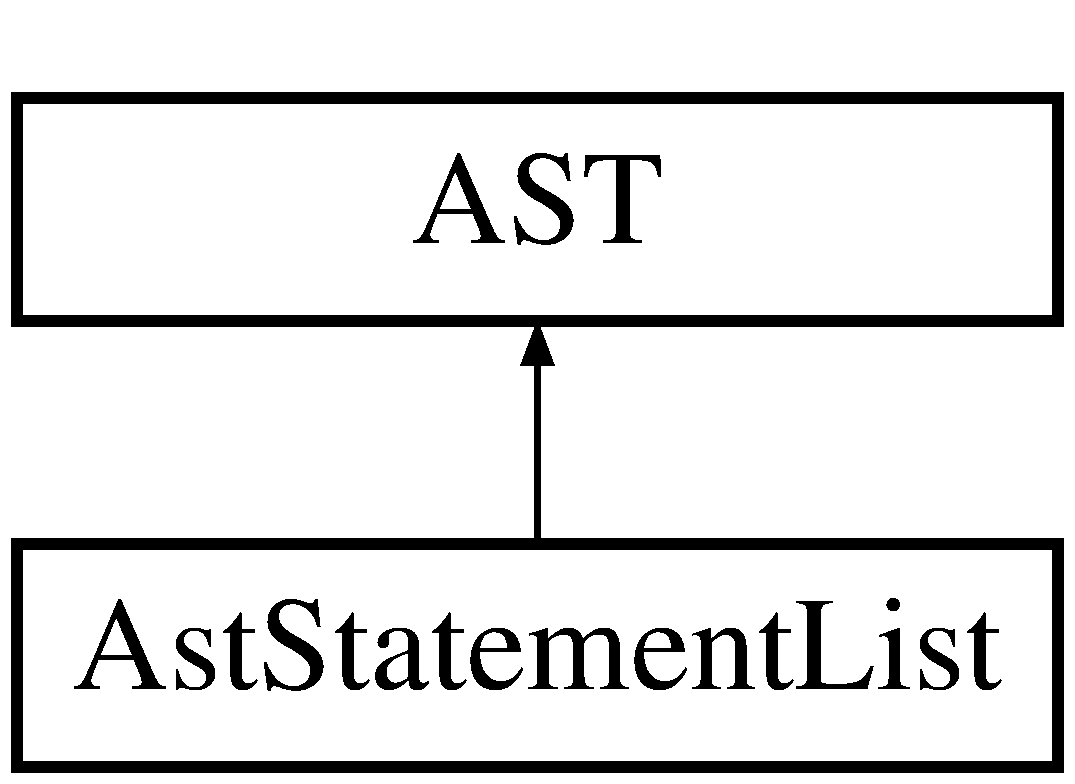
\includegraphics[height=2.000000cm]{classAstStatementList}
\end{center}
\end{figure}
\subsection*{Public Member Functions}
\begin{DoxyCompactItemize}
\item 
\hypertarget{classAstStatementList_a4ac59b2b83022bdbdc5185b0c03688cd}{{\bfseries Ast\-Statement\-List} (\hyperlink{classAstStatement}{Ast\-Statement} $\ast$s)}\label{classAstStatementList_a4ac59b2b83022bdbdc5185b0c03688cd}

\item 
\hypertarget{classAstStatementList_abbf3a704a21fbecef5f4ce1be24449b3}{{\bfseries Ast\-Statement\-List} (\hyperlink{classAstStatementList}{Ast\-Statement\-List} $\ast$l, \hyperlink{classAstStatement}{Ast\-Statement} $\ast$s)}\label{classAstStatementList_abbf3a704a21fbecef5f4ce1be24449b3}

\item 
void \hyperlink{classAstStatementList_a3390e533f15c418a597e1eb3b2a14b99}{Visit} ()
\begin{DoxyCompactList}\small\item\em This function is responsible for tree traversals. \end{DoxyCompactList}\item 
\hypertarget{classAstStatementList_a4ac59b2b83022bdbdc5185b0c03688cd}{{\bfseries Ast\-Statement\-List} (\hyperlink{classAstStatement}{Ast\-Statement} $\ast$s)}\label{classAstStatementList_a4ac59b2b83022bdbdc5185b0c03688cd}

\item 
\hypertarget{classAstStatementList_abbf3a704a21fbecef5f4ce1be24449b3}{{\bfseries Ast\-Statement\-List} (\hyperlink{classAstStatementList}{Ast\-Statement\-List} $\ast$l, \hyperlink{classAstStatement}{Ast\-Statement} $\ast$s)}\label{classAstStatementList_abbf3a704a21fbecef5f4ce1be24449b3}

\item 
void \hyperlink{classAstStatementList_a3390e533f15c418a597e1eb3b2a14b99}{Visit} ()
\begin{DoxyCompactList}\small\item\em This function is responsible for tree traversals. \end{DoxyCompactList}\item 
\hypertarget{classAstStatementList_a4ac59b2b83022bdbdc5185b0c03688cd}{{\bfseries Ast\-Statement\-List} (\hyperlink{classAstStatement}{Ast\-Statement} $\ast$s)}\label{classAstStatementList_a4ac59b2b83022bdbdc5185b0c03688cd}

\item 
\hypertarget{classAstStatementList_abbf3a704a21fbecef5f4ce1be24449b3}{{\bfseries Ast\-Statement\-List} (\hyperlink{classAstStatementList}{Ast\-Statement\-List} $\ast$l, \hyperlink{classAstStatement}{Ast\-Statement} $\ast$s)}\label{classAstStatementList_abbf3a704a21fbecef5f4ce1be24449b3}

\item 
void \hyperlink{classAstStatementList_a3390e533f15c418a597e1eb3b2a14b99}{Visit} ()
\begin{DoxyCompactList}\small\item\em This function is responsible for tree traversals. \end{DoxyCompactList}\item 
\hypertarget{classAstStatementList_a4ac59b2b83022bdbdc5185b0c03688cd}{{\bfseries Ast\-Statement\-List} (\hyperlink{classAstStatement}{Ast\-Statement} $\ast$s)}\label{classAstStatementList_a4ac59b2b83022bdbdc5185b0c03688cd}

\item 
\hypertarget{classAstStatementList_abbf3a704a21fbecef5f4ce1be24449b3}{{\bfseries Ast\-Statement\-List} (\hyperlink{classAstStatementList}{Ast\-Statement\-List} $\ast$l, \hyperlink{classAstStatement}{Ast\-Statement} $\ast$s)}\label{classAstStatementList_abbf3a704a21fbecef5f4ce1be24449b3}

\item 
void \hyperlink{classAstStatementList_a3390e533f15c418a597e1eb3b2a14b99}{Visit} ()
\begin{DoxyCompactList}\small\item\em This function is responsible for tree traversals. \end{DoxyCompactList}\item 
void \hyperlink{classAST_a71d680856e95ff89f55d5311a552eba6}{set\-Label} (string l)
\begin{DoxyCompactList}\small\item\em Sets the label for the node. \end{DoxyCompactList}\item 
void \hyperlink{classAST_a71d680856e95ff89f55d5311a552eba6}{set\-Label} (string l)
\begin{DoxyCompactList}\small\item\em Sets the label for the node. \end{DoxyCompactList}\item 
void \hyperlink{classAST_a71d680856e95ff89f55d5311a552eba6}{set\-Label} (string l)
\begin{DoxyCompactList}\small\item\em Sets the label for the node. \end{DoxyCompactList}\item 
void \hyperlink{classAST_a71d680856e95ff89f55d5311a552eba6}{set\-Label} (string l)
\begin{DoxyCompactList}\small\item\em Sets the label for the node. \end{DoxyCompactList}\item 
int \hyperlink{classAST_ab7a5b1d9f1c2de0d98deb356f724a42c}{get\-U\-I\-D} ()
\begin{DoxyCompactList}\small\item\em Gets the node's unique I\-D. \end{DoxyCompactList}\item 
int \hyperlink{classAST_ab7a5b1d9f1c2de0d98deb356f724a42c}{get\-U\-I\-D} ()
\begin{DoxyCompactList}\small\item\em Gets the node's unique I\-D. \end{DoxyCompactList}\item 
int \hyperlink{classAST_ab7a5b1d9f1c2de0d98deb356f724a42c}{get\-U\-I\-D} ()
\begin{DoxyCompactList}\small\item\em Gets the node's unique I\-D. \end{DoxyCompactList}\item 
int \hyperlink{classAST_ab7a5b1d9f1c2de0d98deb356f724a42c}{get\-U\-I\-D} ()
\begin{DoxyCompactList}\small\item\em Gets the node's unique I\-D. \end{DoxyCompactList}\item 
string \hyperlink{classAST_aee029be902fffc927d16ccb03eb922ad}{get\-Label} ()
\begin{DoxyCompactList}\small\item\em Gets the node's label. \end{DoxyCompactList}\item 
string \hyperlink{classAST_aee029be902fffc927d16ccb03eb922ad}{get\-Label} ()
\begin{DoxyCompactList}\small\item\em Gets the node's label. \end{DoxyCompactList}\item 
string \hyperlink{classAST_aee029be902fffc927d16ccb03eb922ad}{get\-Label} ()
\begin{DoxyCompactList}\small\item\em Gets the node's label. \end{DoxyCompactList}\item 
string \hyperlink{classAST_aee029be902fffc927d16ccb03eb922ad}{get\-Label} ()
\begin{DoxyCompactList}\small\item\em Gets the node's label. \end{DoxyCompactList}\end{DoxyCompactItemize}
\subsection*{Public Attributes}
\begin{DoxyCompactItemize}
\item 
\hypertarget{classAST_aaf215802de409f8096c063d01ffa6783}{bool \hyperlink{classAST_aaf215802de409f8096c063d01ffa6783}{needs\-Cast}}\label{classAST_aaf215802de409f8096c063d01ffa6783}

\begin{DoxyCompactList}\small\item\em This indicates if cast 3\-A\-C needs to be output, and is only relevant for expressions. \end{DoxyCompactList}\item 
\hypertarget{classAST_afa9e77ef650ec6664458fa6cb55be985}{bool \hyperlink{classAST_afa9e77ef650ec6664458fa6cb55be985}{is\-Conv}}\label{classAST_afa9e77ef650ec6664458fa6cb55be985}

\begin{DoxyCompactList}\small\item\em Indicates is a conversion is possible. \end{DoxyCompactList}\item 
\hypertarget{classAST_a61ef3317e023d45237e06615b387cd6b}{C\-O\-N\-V\-E\-R\-S\-I\-O\-N\-T\-Y\-P\-E \hyperlink{classAST_a61ef3317e023d45237e06615b387cd6b}{conv\-Type}}\label{classAST_a61ef3317e023d45237e06615b387cd6b}

\begin{DoxyCompactList}\small\item\em If needs\-Cast is true, then this indicates what the cast should be. \end{DoxyCompactList}\item 
\hypertarget{classAST_aea9b07b39d24183f38c0029cec0a878e}{int \hyperlink{classAST_aea9b07b39d24183f38c0029cec0a878e}{operand\-To\-Cast}}\label{classAST_aea9b07b39d24183f38c0029cec0a878e}

\begin{DoxyCompactList}\small\item\em This indicates if the first or second operand should be the one that is cast. \end{DoxyCompactList}\end{DoxyCompactItemize}
\subsection*{Static Public Attributes}
\begin{DoxyCompactItemize}
\item 
\hypertarget{classAST_a5fdfd5f7b104dd92889163bdadbc68d6}{static \hyperlink{classVisualizer}{Visualizer} \hyperlink{classAST_a5fdfd5f7b104dd92889163bdadbc68d6}{vis}}\label{classAST_a5fdfd5f7b104dd92889163bdadbc68d6}

\begin{DoxyCompactList}\small\item\em Static visualizer instance for generating the visualization of the \hyperlink{classAST}{A\-S\-T}. \end{DoxyCompactList}\item 
\hypertarget{classAST_a8a3ace322f50e030331065d644ee55ee}{static \hyperlink{classTAC__Generator}{T\-A\-C\-\_\-\-Generator} \hyperlink{classAST_a8a3ace322f50e030331065d644ee55ee}{tac\-Gen}}\label{classAST_a8a3ace322f50e030331065d644ee55ee}

\begin{DoxyCompactList}\small\item\em Three address code generator. \end{DoxyCompactList}\item 
\hypertarget{classAST_a1f69448c6dc368d005631a128460083d}{static string {\bfseries current\-Temp} =\char`\"{}\char`\"{}}\label{classAST_a1f69448c6dc368d005631a128460083d}

\item 
\hypertarget{classAST_a551aec090c932ab69365238b40a8a4eb}{static string \hyperlink{classAST_a551aec090c932ab69365238b40a8a4eb}{return\-Label} =\char`\"{}\char`\"{}}\label{classAST_a551aec090c932ab69365238b40a8a4eb}

\begin{DoxyCompactList}\small\item\em This is for storing the string id of any temporary result register that may be created during 3\-A\-C generation. \end{DoxyCompactList}\item 
\hypertarget{classAST_a73c0a266df52be71e6b527b6aa635173}{static list$<$ string $>$ {\bfseries temp\-Stack}}\label{classAST_a73c0a266df52be71e6b527b6aa635173}

\item 
\hypertarget{classAST_abf9e84b541ff04b7bb64e6e4371512d4}{static string {\bfseries last\-I\-D} =\char`\"{}\char`\"{}}\label{classAST_abf9e84b541ff04b7bb64e6e4371512d4}

\item 
\hypertarget{classAST_a163003bfe9c30510ec8039870346049f}{static \hyperlink{classSymTab}{Sym\-Tab} $\ast$ {\bfseries symbol\-Table} =N\-U\-L\-L}\label{classAST_a163003bfe9c30510ec8039870346049f}

\item 
\hypertarget{classAST_a5c3cc894d9c0453523dec9ed76f18a04}{static string {\bfseries current\-Function} =\char`\"{}\char`\"{}}\label{classAST_a5c3cc894d9c0453523dec9ed76f18a04}

\item 
\hypertarget{classAST_a66155513b59ff1a04c8ece8b20ec31f5}{static int {\bfseries current\-Constant\-Value} =0}\label{classAST_a66155513b59ff1a04c8ece8b20ec31f5}

\item 
\hypertarget{classAST_a3d031d7bab635ba1f015aade5943f40c}{static string {\bfseries current\-Id\-Name} =\char`\"{}\char`\"{}}\label{classAST_a3d031d7bab635ba1f015aade5943f40c}

\item 
\hypertarget{classAST_a16c4b6e54febc1a26b31a64a46972ef0}{static int {\bfseries current\-Index\-Val} = 0}\label{classAST_a16c4b6e54febc1a26b31a64a46972ef0}

\end{DoxyCompactItemize}
\subsection*{Protected Attributes}
\begin{DoxyCompactItemize}
\item 
\hypertarget{classAST_a847b778f1c3dd5a19de32de432ee6e15}{int \hyperlink{classAST_a847b778f1c3dd5a19de32de432ee6e15}{uid}}\label{classAST_a847b778f1c3dd5a19de32de432ee6e15}

\begin{DoxyCompactList}\small\item\em The unique id. \end{DoxyCompactList}\item 
\hypertarget{classAST_ab2e239ccc0688d2341724432ff5a1a31}{string \hyperlink{classAST_ab2e239ccc0688d2341724432ff5a1a31}{label}}\label{classAST_ab2e239ccc0688d2341724432ff5a1a31}

\begin{DoxyCompactList}\small\item\em The label to be printed in the visualization. \end{DoxyCompactList}\end{DoxyCompactItemize}
\subsection*{Private Attributes}
\begin{DoxyCompactItemize}
\item 
\hypertarget{classAstStatementList_afe22f7c75e95ec82d3b120c197204faa}{\hyperlink{classAstStatement}{Ast\-Statement} $\ast$ {\bfseries stmt}}\label{classAstStatementList_afe22f7c75e95ec82d3b120c197204faa}

\item 
\hypertarget{classAstStatementList_a926c32788d327bda01a3ae64bf7a33a6}{\hyperlink{classAstStatementList}{Ast\-Statement\-List} $\ast$ {\bfseries list}}\label{classAstStatementList_a926c32788d327bda01a3ae64bf7a33a6}

\end{DoxyCompactItemize}


\subsection{Detailed Description}


Definition at line 1291 of file Ast.\-h.



\subsection{Member Function Documentation}
\hypertarget{classAST_aee029be902fffc927d16ccb03eb922ad}{\index{Ast\-Statement\-List@{Ast\-Statement\-List}!get\-Label@{get\-Label}}
\index{get\-Label@{get\-Label}!AstStatementList@{Ast\-Statement\-List}}
\subsubsection[{get\-Label}]{\setlength{\rightskip}{0pt plus 5cm}string A\-S\-T\-::get\-Label (
\begin{DoxyParamCaption}
{}
\end{DoxyParamCaption}
)\hspace{0.3cm}{\ttfamily [inline]}, {\ttfamily [inherited]}}}\label{classAST_aee029be902fffc927d16ccb03eb922ad}


Gets the node's label. 

\begin{DoxyReturn}{Returns}
The label 
\end{DoxyReturn}


Definition at line 60 of file Ast.\-h.

\hypertarget{classAST_aee029be902fffc927d16ccb03eb922ad}{\index{Ast\-Statement\-List@{Ast\-Statement\-List}!get\-Label@{get\-Label}}
\index{get\-Label@{get\-Label}!AstStatementList@{Ast\-Statement\-List}}
\subsubsection[{get\-Label}]{\setlength{\rightskip}{0pt plus 5cm}string A\-S\-T\-::get\-Label (
\begin{DoxyParamCaption}
{}
\end{DoxyParamCaption}
)\hspace{0.3cm}{\ttfamily [inline]}, {\ttfamily [inherited]}}}\label{classAST_aee029be902fffc927d16ccb03eb922ad}


Gets the node's label. 

\begin{DoxyReturn}{Returns}
The label 
\end{DoxyReturn}


Definition at line 60 of file C\-Scanner.\-ll.

\hypertarget{classAST_aee029be902fffc927d16ccb03eb922ad}{\index{Ast\-Statement\-List@{Ast\-Statement\-List}!get\-Label@{get\-Label}}
\index{get\-Label@{get\-Label}!AstStatementList@{Ast\-Statement\-List}}
\subsubsection[{get\-Label}]{\setlength{\rightskip}{0pt plus 5cm}string A\-S\-T\-::get\-Label (
\begin{DoxyParamCaption}
{}
\end{DoxyParamCaption}
)\hspace{0.3cm}{\ttfamily [inline]}, {\ttfamily [inherited]}}}\label{classAST_aee029be902fffc927d16ccb03eb922ad}


Gets the node's label. 

\begin{DoxyReturn}{Returns}
The label 
\end{DoxyReturn}


Definition at line 60 of file C\-Parser.\-yy.

\hypertarget{classAST_aee029be902fffc927d16ccb03eb922ad}{\index{Ast\-Statement\-List@{Ast\-Statement\-List}!get\-Label@{get\-Label}}
\index{get\-Label@{get\-Label}!AstStatementList@{Ast\-Statement\-List}}
\subsubsection[{get\-Label}]{\setlength{\rightskip}{0pt plus 5cm}string A\-S\-T\-::get\-Label (
\begin{DoxyParamCaption}
{}
\end{DoxyParamCaption}
)\hspace{0.3cm}{\ttfamily [inline]}, {\ttfamily [inherited]}}}\label{classAST_aee029be902fffc927d16ccb03eb922ad}


Gets the node's label. 

\begin{DoxyReturn}{Returns}
The label 
\end{DoxyReturn}


Definition at line 60 of file C\-Parser.\-yy.

\hypertarget{classAST_ab7a5b1d9f1c2de0d98deb356f724a42c}{\index{Ast\-Statement\-List@{Ast\-Statement\-List}!get\-U\-I\-D@{get\-U\-I\-D}}
\index{get\-U\-I\-D@{get\-U\-I\-D}!AstStatementList@{Ast\-Statement\-List}}
\subsubsection[{get\-U\-I\-D}]{\setlength{\rightskip}{0pt plus 5cm}int A\-S\-T\-::get\-U\-I\-D (
\begin{DoxyParamCaption}
{}
\end{DoxyParamCaption}
)\hspace{0.3cm}{\ttfamily [inline]}, {\ttfamily [inherited]}}}\label{classAST_ab7a5b1d9f1c2de0d98deb356f724a42c}


Gets the node's unique I\-D. 

\begin{DoxyReturn}{Returns}
The unique id 
\end{DoxyReturn}


Definition at line 53 of file C\-Parser.\-yy.

\hypertarget{classAST_ab7a5b1d9f1c2de0d98deb356f724a42c}{\index{Ast\-Statement\-List@{Ast\-Statement\-List}!get\-U\-I\-D@{get\-U\-I\-D}}
\index{get\-U\-I\-D@{get\-U\-I\-D}!AstStatementList@{Ast\-Statement\-List}}
\subsubsection[{get\-U\-I\-D}]{\setlength{\rightskip}{0pt plus 5cm}int A\-S\-T\-::get\-U\-I\-D (
\begin{DoxyParamCaption}
{}
\end{DoxyParamCaption}
)\hspace{0.3cm}{\ttfamily [inline]}, {\ttfamily [inherited]}}}\label{classAST_ab7a5b1d9f1c2de0d98deb356f724a42c}


Gets the node's unique I\-D. 

\begin{DoxyReturn}{Returns}
The unique id 
\end{DoxyReturn}


Definition at line 53 of file C\-Parser.\-yy.

\hypertarget{classAST_ab7a5b1d9f1c2de0d98deb356f724a42c}{\index{Ast\-Statement\-List@{Ast\-Statement\-List}!get\-U\-I\-D@{get\-U\-I\-D}}
\index{get\-U\-I\-D@{get\-U\-I\-D}!AstStatementList@{Ast\-Statement\-List}}
\subsubsection[{get\-U\-I\-D}]{\setlength{\rightskip}{0pt plus 5cm}int A\-S\-T\-::get\-U\-I\-D (
\begin{DoxyParamCaption}
{}
\end{DoxyParamCaption}
)\hspace{0.3cm}{\ttfamily [inline]}, {\ttfamily [inherited]}}}\label{classAST_ab7a5b1d9f1c2de0d98deb356f724a42c}


Gets the node's unique I\-D. 

\begin{DoxyReturn}{Returns}
The unique id 
\end{DoxyReturn}


Definition at line 53 of file C\-Scanner.\-ll.

\hypertarget{classAST_ab7a5b1d9f1c2de0d98deb356f724a42c}{\index{Ast\-Statement\-List@{Ast\-Statement\-List}!get\-U\-I\-D@{get\-U\-I\-D}}
\index{get\-U\-I\-D@{get\-U\-I\-D}!AstStatementList@{Ast\-Statement\-List}}
\subsubsection[{get\-U\-I\-D}]{\setlength{\rightskip}{0pt plus 5cm}int A\-S\-T\-::get\-U\-I\-D (
\begin{DoxyParamCaption}
{}
\end{DoxyParamCaption}
)\hspace{0.3cm}{\ttfamily [inline]}, {\ttfamily [inherited]}}}\label{classAST_ab7a5b1d9f1c2de0d98deb356f724a42c}


Gets the node's unique I\-D. 

\begin{DoxyReturn}{Returns}
The unique id 
\end{DoxyReturn}


Definition at line 53 of file Ast.\-h.

\hypertarget{classAST_a71d680856e95ff89f55d5311a552eba6}{\index{Ast\-Statement\-List@{Ast\-Statement\-List}!set\-Label@{set\-Label}}
\index{set\-Label@{set\-Label}!AstStatementList@{Ast\-Statement\-List}}
\subsubsection[{set\-Label}]{\setlength{\rightskip}{0pt plus 5cm}void A\-S\-T\-::set\-Label (
\begin{DoxyParamCaption}
\item[{string}]{l}
\end{DoxyParamCaption}
)\hspace{0.3cm}{\ttfamily [inline]}, {\ttfamily [inherited]}}}\label{classAST_a71d680856e95ff89f55d5311a552eba6}


Sets the label for the node. 


\begin{DoxyParams}{Parameters}
{\em l} & The label string \\
\hline
\end{DoxyParams}


Definition at line 43 of file C\-Scanner.\-ll.

\hypertarget{classAST_a71d680856e95ff89f55d5311a552eba6}{\index{Ast\-Statement\-List@{Ast\-Statement\-List}!set\-Label@{set\-Label}}
\index{set\-Label@{set\-Label}!AstStatementList@{Ast\-Statement\-List}}
\subsubsection[{set\-Label}]{\setlength{\rightskip}{0pt plus 5cm}void A\-S\-T\-::set\-Label (
\begin{DoxyParamCaption}
\item[{string}]{l}
\end{DoxyParamCaption}
)\hspace{0.3cm}{\ttfamily [inline]}, {\ttfamily [inherited]}}}\label{classAST_a71d680856e95ff89f55d5311a552eba6}


Sets the label for the node. 


\begin{DoxyParams}{Parameters}
{\em l} & The label string \\
\hline
\end{DoxyParams}


Definition at line 43 of file C\-Parser.\-yy.

\hypertarget{classAST_a71d680856e95ff89f55d5311a552eba6}{\index{Ast\-Statement\-List@{Ast\-Statement\-List}!set\-Label@{set\-Label}}
\index{set\-Label@{set\-Label}!AstStatementList@{Ast\-Statement\-List}}
\subsubsection[{set\-Label}]{\setlength{\rightskip}{0pt plus 5cm}void A\-S\-T\-::set\-Label (
\begin{DoxyParamCaption}
\item[{string}]{l}
\end{DoxyParamCaption}
)\hspace{0.3cm}{\ttfamily [inline]}, {\ttfamily [inherited]}}}\label{classAST_a71d680856e95ff89f55d5311a552eba6}


Sets the label for the node. 


\begin{DoxyParams}{Parameters}
{\em l} & The label string \\
\hline
\end{DoxyParams}


Definition at line 43 of file Ast.\-h.

\hypertarget{classAST_a71d680856e95ff89f55d5311a552eba6}{\index{Ast\-Statement\-List@{Ast\-Statement\-List}!set\-Label@{set\-Label}}
\index{set\-Label@{set\-Label}!AstStatementList@{Ast\-Statement\-List}}
\subsubsection[{set\-Label}]{\setlength{\rightskip}{0pt plus 5cm}void A\-S\-T\-::set\-Label (
\begin{DoxyParamCaption}
\item[{string}]{l}
\end{DoxyParamCaption}
)\hspace{0.3cm}{\ttfamily [inline]}, {\ttfamily [inherited]}}}\label{classAST_a71d680856e95ff89f55d5311a552eba6}


Sets the label for the node. 


\begin{DoxyParams}{Parameters}
{\em l} & The label string \\
\hline
\end{DoxyParams}


Definition at line 43 of file C\-Parser.\-yy.

\hypertarget{classAstStatementList_a3390e533f15c418a597e1eb3b2a14b99}{\index{Ast\-Statement\-List@{Ast\-Statement\-List}!Visit@{Visit}}
\index{Visit@{Visit}!AstStatementList@{Ast\-Statement\-List}}
\subsubsection[{Visit}]{\setlength{\rightskip}{0pt plus 5cm}void Ast\-Statement\-List\-::\-Visit (
\begin{DoxyParamCaption}
{}
\end{DoxyParamCaption}
)\hspace{0.3cm}{\ttfamily [virtual]}}}\label{classAstStatementList_a3390e533f15c418a597e1eb3b2a14b99}


This function is responsible for tree traversals. 

This function will call the Visit functions of each of it's children nodes, call the visualization code for itself, and output any 3\-A\-C that can be generated at the current node. 

Reimplemented from \hyperlink{classAST_a5828cc86f2c4f1a0aeab6d7069e8fd82}{A\-S\-T}.



Definition at line 2586 of file Ast.\-cpp.

\hypertarget{classAstStatementList_a3390e533f15c418a597e1eb3b2a14b99}{\index{Ast\-Statement\-List@{Ast\-Statement\-List}!Visit@{Visit}}
\index{Visit@{Visit}!AstStatementList@{Ast\-Statement\-List}}
\subsubsection[{Visit}]{\setlength{\rightskip}{0pt plus 5cm}void Ast\-Statement\-List\-::\-Visit (
\begin{DoxyParamCaption}
{}
\end{DoxyParamCaption}
)\hspace{0.3cm}{\ttfamily [virtual]}}}\label{classAstStatementList_a3390e533f15c418a597e1eb3b2a14b99}


This function is responsible for tree traversals. 

This function will call the Visit functions of each of it's children nodes, call the visualization code for itself, and output any 3\-A\-C that can be generated at the current node. 

Reimplemented from \hyperlink{classAST_a5828cc86f2c4f1a0aeab6d7069e8fd82}{A\-S\-T}.

\hypertarget{classAstStatementList_a3390e533f15c418a597e1eb3b2a14b99}{\index{Ast\-Statement\-List@{Ast\-Statement\-List}!Visit@{Visit}}
\index{Visit@{Visit}!AstStatementList@{Ast\-Statement\-List}}
\subsubsection[{Visit}]{\setlength{\rightskip}{0pt plus 5cm}void Ast\-Statement\-List\-::\-Visit (
\begin{DoxyParamCaption}
{}
\end{DoxyParamCaption}
)\hspace{0.3cm}{\ttfamily [virtual]}}}\label{classAstStatementList_a3390e533f15c418a597e1eb3b2a14b99}


This function is responsible for tree traversals. 

This function will call the Visit functions of each of it's children nodes, call the visualization code for itself, and output any 3\-A\-C that can be generated at the current node. 

Reimplemented from \hyperlink{classAST_a5828cc86f2c4f1a0aeab6d7069e8fd82}{A\-S\-T}.

\hypertarget{classAstStatementList_a3390e533f15c418a597e1eb3b2a14b99}{\index{Ast\-Statement\-List@{Ast\-Statement\-List}!Visit@{Visit}}
\index{Visit@{Visit}!AstStatementList@{Ast\-Statement\-List}}
\subsubsection[{Visit}]{\setlength{\rightskip}{0pt plus 5cm}void Ast\-Statement\-List\-::\-Visit (
\begin{DoxyParamCaption}
{}
\end{DoxyParamCaption}
)\hspace{0.3cm}{\ttfamily [virtual]}}}\label{classAstStatementList_a3390e533f15c418a597e1eb3b2a14b99}


This function is responsible for tree traversals. 

This function will call the Visit functions of each of it's children nodes, call the visualization code for itself, and output any 3\-A\-C that can be generated at the current node. 

Reimplemented from \hyperlink{classAST_a5828cc86f2c4f1a0aeab6d7069e8fd82}{A\-S\-T}.



The documentation for this class was generated from the following files\-:\begin{DoxyCompactItemize}
\item 
Ast.\-h\item 
Ast.\-cpp\end{DoxyCompactItemize}

\hypertarget{classAstString}{\section{Ast\-String Class Reference}
\label{classAstString}\index{Ast\-String@{Ast\-String}}
}
Inheritance diagram for Ast\-String\-:\begin{figure}[H]
\begin{center}
\leavevmode
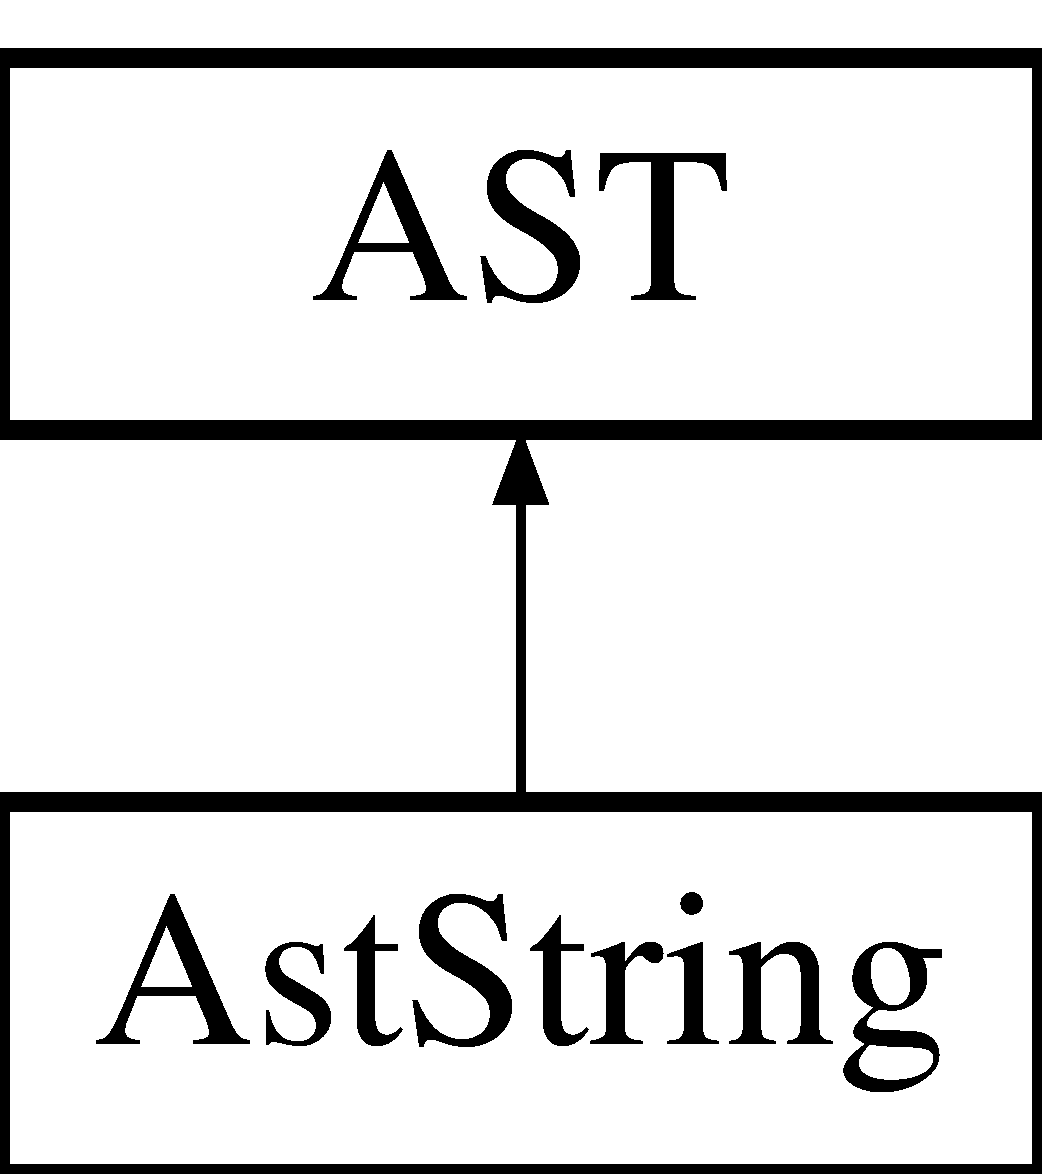
\includegraphics[height=2.000000cm]{classAstString}
\end{center}
\end{figure}
\subsection*{Public Member Functions}
\begin{DoxyCompactItemize}
\item 
\hypertarget{classAstString_a7a4dfa0949d876400dc288b299274d51}{{\bfseries Ast\-String} (string str)}\label{classAstString_a7a4dfa0949d876400dc288b299274d51}

\item 
void \hyperlink{classAstString_a0a7a6576cf72bfbcd2f78c7ffb9350bb}{Visit} ()
\begin{DoxyCompactList}\small\item\em This function is responsible for tree traversals. \end{DoxyCompactList}\item 
void \hyperlink{classAST_a71d680856e95ff89f55d5311a552eba6}{set\-Label} (string l)
\begin{DoxyCompactList}\small\item\em Sets the label for the node. \end{DoxyCompactList}\item 
int \hyperlink{classAST_ab7a5b1d9f1c2de0d98deb356f724a42c}{get\-U\-I\-D} ()
\begin{DoxyCompactList}\small\item\em Gets the node's unique I\-D. \end{DoxyCompactList}\item 
string \hyperlink{classAST_aee029be902fffc927d16ccb03eb922ad}{get\-Label} ()
\begin{DoxyCompactList}\small\item\em Gets the node's label. \end{DoxyCompactList}\end{DoxyCompactItemize}
\subsection*{Static Public Attributes}
\begin{DoxyCompactItemize}
\item 
\hypertarget{classAST_aca9e6637209b31e03a09c0d42f29bdfa}{static \hyperlink{classVisualizer}{Visualizer} \hyperlink{classAST_aca9e6637209b31e03a09c0d42f29bdfa}{vis}}\label{classAST_aca9e6637209b31e03a09c0d42f29bdfa}

\begin{DoxyCompactList}\small\item\em Static visualizer instance for generating the visualization of the \hyperlink{classAST}{A\-S\-T}. \end{DoxyCompactList}\end{DoxyCompactItemize}
\subsection*{Protected Attributes}
\begin{DoxyCompactItemize}
\item 
\hypertarget{classAST_a847b778f1c3dd5a19de32de432ee6e15}{int \hyperlink{classAST_a847b778f1c3dd5a19de32de432ee6e15}{uid}}\label{classAST_a847b778f1c3dd5a19de32de432ee6e15}

\begin{DoxyCompactList}\small\item\em The unique id. \end{DoxyCompactList}\item 
\hypertarget{classAST_ab2e239ccc0688d2341724432ff5a1a31}{string \hyperlink{classAST_ab2e239ccc0688d2341724432ff5a1a31}{label}}\label{classAST_ab2e239ccc0688d2341724432ff5a1a31}

\begin{DoxyCompactList}\small\item\em The label to be printed in the visualization. \end{DoxyCompactList}\end{DoxyCompactItemize}
\subsection*{Private Attributes}
\begin{DoxyCompactItemize}
\item 
\hypertarget{classAstString_a6ea56d675adc723bd86ab5e8393db7c8}{string {\bfseries val}}\label{classAstString_a6ea56d675adc723bd86ab5e8393db7c8}

\end{DoxyCompactItemize}


\subsection{Member Function Documentation}
\hypertarget{classAST_aee029be902fffc927d16ccb03eb922ad}{\index{Ast\-String@{Ast\-String}!get\-Label@{get\-Label}}
\index{get\-Label@{get\-Label}!AstString@{Ast\-String}}
\subsubsection[{get\-Label}]{\setlength{\rightskip}{0pt plus 5cm}string A\-S\-T\-::get\-Label (
\begin{DoxyParamCaption}
{}
\end{DoxyParamCaption}
)\hspace{0.3cm}{\ttfamily [inline]}, {\ttfamily [inherited]}}}\label{classAST_aee029be902fffc927d16ccb03eb922ad}


Gets the node's label. 

\begin{DoxyReturn}{Returns}
The label 
\end{DoxyReturn}
\hypertarget{classAST_ab7a5b1d9f1c2de0d98deb356f724a42c}{\index{Ast\-String@{Ast\-String}!get\-U\-I\-D@{get\-U\-I\-D}}
\index{get\-U\-I\-D@{get\-U\-I\-D}!AstString@{Ast\-String}}
\subsubsection[{get\-U\-I\-D}]{\setlength{\rightskip}{0pt plus 5cm}int A\-S\-T\-::get\-U\-I\-D (
\begin{DoxyParamCaption}
{}
\end{DoxyParamCaption}
)\hspace{0.3cm}{\ttfamily [inline]}, {\ttfamily [inherited]}}}\label{classAST_ab7a5b1d9f1c2de0d98deb356f724a42c}


Gets the node's unique I\-D. 

\begin{DoxyReturn}{Returns}
The unique id 
\end{DoxyReturn}
\hypertarget{classAST_a71d680856e95ff89f55d5311a552eba6}{\index{Ast\-String@{Ast\-String}!set\-Label@{set\-Label}}
\index{set\-Label@{set\-Label}!AstString@{Ast\-String}}
\subsubsection[{set\-Label}]{\setlength{\rightskip}{0pt plus 5cm}void A\-S\-T\-::set\-Label (
\begin{DoxyParamCaption}
\item[{string}]{l}
\end{DoxyParamCaption}
)\hspace{0.3cm}{\ttfamily [inline]}, {\ttfamily [inherited]}}}\label{classAST_a71d680856e95ff89f55d5311a552eba6}


Sets the label for the node. 


\begin{DoxyParams}{Parameters}
{\em l} & The label string \\
\hline
\end{DoxyParams}
\hypertarget{classAstString_a0a7a6576cf72bfbcd2f78c7ffb9350bb}{\index{Ast\-String@{Ast\-String}!Visit@{Visit}}
\index{Visit@{Visit}!AstString@{Ast\-String}}
\subsubsection[{Visit}]{\setlength{\rightskip}{0pt plus 5cm}void Ast\-String\-::\-Visit (
\begin{DoxyParamCaption}
{}
\end{DoxyParamCaption}
)\hspace{0.3cm}{\ttfamily [virtual]}}}\label{classAstString_a0a7a6576cf72bfbcd2f78c7ffb9350bb}


This function is responsible for tree traversals. 

This function will call the Visit functions of each of it's children nodes, call the visualization code for itself, and output any 3\-A\-C that can be generated at the current node. 

Reimplemented from \hyperlink{classAST_a5828cc86f2c4f1a0aeab6d7069e8fd82}{A\-S\-T}.



The documentation for this class was generated from the following files\-:\begin{DoxyCompactItemize}
\item 
Ast.\-h\item 
Ast.\-cpp\end{DoxyCompactItemize}

\input{classAstStructDecl}
\input{classAstStructDeclarator}
\input{classAstStructDeclatorList}
\input{classAstStructDeclList}
\input{classAstStructUniSpeci}
\hypertarget{classAstSwitch}{\section{Ast\-Switch Class Reference}
\label{classAstSwitch}\index{Ast\-Switch@{Ast\-Switch}}
}
Inheritance diagram for Ast\-Switch\-:\begin{figure}[H]
\begin{center}
\leavevmode
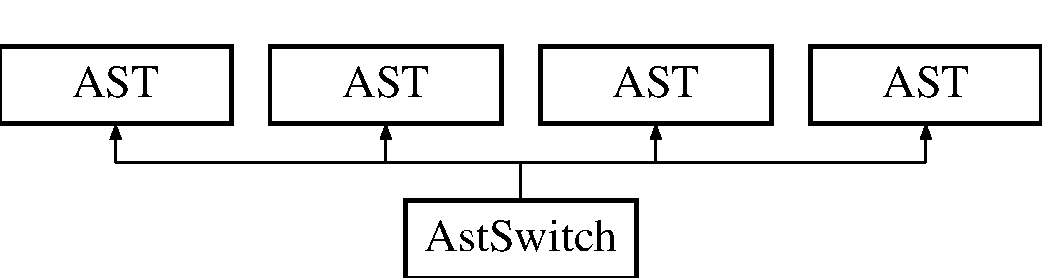
\includegraphics[height=2.000000cm]{classAstSwitch}
\end{center}
\end{figure}
\subsection*{Public Member Functions}
\begin{DoxyCompactItemize}
\item 
\hypertarget{classAstSwitch_a5a11f2c6bbed34a0deb5a150e8e53978}{{\bfseries Ast\-Switch} (\hyperlink{classAstExpression}{Ast\-Expression} $\ast$e, \hyperlink{classAstStatement}{Ast\-Statement} $\ast$s)}\label{classAstSwitch_a5a11f2c6bbed34a0deb5a150e8e53978}

\item 
void \hyperlink{classAstSwitch_a12d5e48474fec08fbf41cb69cffd740a}{Visit} ()
\begin{DoxyCompactList}\small\item\em This function is responsible for tree traversals. \end{DoxyCompactList}\item 
\hypertarget{classAstSwitch_a5a11f2c6bbed34a0deb5a150e8e53978}{{\bfseries Ast\-Switch} (\hyperlink{classAstExpression}{Ast\-Expression} $\ast$e, \hyperlink{classAstStatement}{Ast\-Statement} $\ast$s)}\label{classAstSwitch_a5a11f2c6bbed34a0deb5a150e8e53978}

\item 
void \hyperlink{classAstSwitch_a12d5e48474fec08fbf41cb69cffd740a}{Visit} ()
\begin{DoxyCompactList}\small\item\em This function is responsible for tree traversals. \end{DoxyCompactList}\item 
\hypertarget{classAstSwitch_a5a11f2c6bbed34a0deb5a150e8e53978}{{\bfseries Ast\-Switch} (\hyperlink{classAstExpression}{Ast\-Expression} $\ast$e, \hyperlink{classAstStatement}{Ast\-Statement} $\ast$s)}\label{classAstSwitch_a5a11f2c6bbed34a0deb5a150e8e53978}

\item 
void \hyperlink{classAstSwitch_a12d5e48474fec08fbf41cb69cffd740a}{Visit} ()
\begin{DoxyCompactList}\small\item\em This function is responsible for tree traversals. \end{DoxyCompactList}\item 
\hypertarget{classAstSwitch_a5a11f2c6bbed34a0deb5a150e8e53978}{{\bfseries Ast\-Switch} (\hyperlink{classAstExpression}{Ast\-Expression} $\ast$e, \hyperlink{classAstStatement}{Ast\-Statement} $\ast$s)}\label{classAstSwitch_a5a11f2c6bbed34a0deb5a150e8e53978}

\item 
void \hyperlink{classAstSwitch_a12d5e48474fec08fbf41cb69cffd740a}{Visit} ()
\begin{DoxyCompactList}\small\item\em This function is responsible for tree traversals. \end{DoxyCompactList}\item 
void \hyperlink{classAST_a71d680856e95ff89f55d5311a552eba6}{set\-Label} (string l)
\begin{DoxyCompactList}\small\item\em Sets the label for the node. \end{DoxyCompactList}\item 
void \hyperlink{classAST_a71d680856e95ff89f55d5311a552eba6}{set\-Label} (string l)
\begin{DoxyCompactList}\small\item\em Sets the label for the node. \end{DoxyCompactList}\item 
void \hyperlink{classAST_a71d680856e95ff89f55d5311a552eba6}{set\-Label} (string l)
\begin{DoxyCompactList}\small\item\em Sets the label for the node. \end{DoxyCompactList}\item 
void \hyperlink{classAST_a71d680856e95ff89f55d5311a552eba6}{set\-Label} (string l)
\begin{DoxyCompactList}\small\item\em Sets the label for the node. \end{DoxyCompactList}\item 
int \hyperlink{classAST_ab7a5b1d9f1c2de0d98deb356f724a42c}{get\-U\-I\-D} ()
\begin{DoxyCompactList}\small\item\em Gets the node's unique I\-D. \end{DoxyCompactList}\item 
int \hyperlink{classAST_ab7a5b1d9f1c2de0d98deb356f724a42c}{get\-U\-I\-D} ()
\begin{DoxyCompactList}\small\item\em Gets the node's unique I\-D. \end{DoxyCompactList}\item 
int \hyperlink{classAST_ab7a5b1d9f1c2de0d98deb356f724a42c}{get\-U\-I\-D} ()
\begin{DoxyCompactList}\small\item\em Gets the node's unique I\-D. \end{DoxyCompactList}\item 
int \hyperlink{classAST_ab7a5b1d9f1c2de0d98deb356f724a42c}{get\-U\-I\-D} ()
\begin{DoxyCompactList}\small\item\em Gets the node's unique I\-D. \end{DoxyCompactList}\item 
string \hyperlink{classAST_aee029be902fffc927d16ccb03eb922ad}{get\-Label} ()
\begin{DoxyCompactList}\small\item\em Gets the node's label. \end{DoxyCompactList}\item 
string \hyperlink{classAST_aee029be902fffc927d16ccb03eb922ad}{get\-Label} ()
\begin{DoxyCompactList}\small\item\em Gets the node's label. \end{DoxyCompactList}\item 
string \hyperlink{classAST_aee029be902fffc927d16ccb03eb922ad}{get\-Label} ()
\begin{DoxyCompactList}\small\item\em Gets the node's label. \end{DoxyCompactList}\item 
string \hyperlink{classAST_aee029be902fffc927d16ccb03eb922ad}{get\-Label} ()
\begin{DoxyCompactList}\small\item\em Gets the node's label. \end{DoxyCompactList}\end{DoxyCompactItemize}
\subsection*{Public Attributes}
\begin{DoxyCompactItemize}
\item 
\hypertarget{classAST_aaf215802de409f8096c063d01ffa6783}{bool \hyperlink{classAST_aaf215802de409f8096c063d01ffa6783}{needs\-Cast}}\label{classAST_aaf215802de409f8096c063d01ffa6783}

\begin{DoxyCompactList}\small\item\em This indicates if cast 3\-A\-C needs to be output, and is only relevant for expressions. \end{DoxyCompactList}\item 
\hypertarget{classAST_afa9e77ef650ec6664458fa6cb55be985}{bool \hyperlink{classAST_afa9e77ef650ec6664458fa6cb55be985}{is\-Conv}}\label{classAST_afa9e77ef650ec6664458fa6cb55be985}

\begin{DoxyCompactList}\small\item\em Indicates is a conversion is possible. \end{DoxyCompactList}\item 
\hypertarget{classAST_a61ef3317e023d45237e06615b387cd6b}{C\-O\-N\-V\-E\-R\-S\-I\-O\-N\-T\-Y\-P\-E \hyperlink{classAST_a61ef3317e023d45237e06615b387cd6b}{conv\-Type}}\label{classAST_a61ef3317e023d45237e06615b387cd6b}

\begin{DoxyCompactList}\small\item\em If needs\-Cast is true, then this indicates what the cast should be. \end{DoxyCompactList}\item 
\hypertarget{classAST_aea9b07b39d24183f38c0029cec0a878e}{int \hyperlink{classAST_aea9b07b39d24183f38c0029cec0a878e}{operand\-To\-Cast}}\label{classAST_aea9b07b39d24183f38c0029cec0a878e}

\begin{DoxyCompactList}\small\item\em This indicates if the first or second operand should be the one that is cast. \end{DoxyCompactList}\end{DoxyCompactItemize}
\subsection*{Static Public Attributes}
\begin{DoxyCompactItemize}
\item 
\hypertarget{classAST_a5fdfd5f7b104dd92889163bdadbc68d6}{static \hyperlink{classVisualizer}{Visualizer} \hyperlink{classAST_a5fdfd5f7b104dd92889163bdadbc68d6}{vis}}\label{classAST_a5fdfd5f7b104dd92889163bdadbc68d6}

\begin{DoxyCompactList}\small\item\em Static visualizer instance for generating the visualization of the \hyperlink{classAST}{A\-S\-T}. \end{DoxyCompactList}\item 
\hypertarget{classAST_a8a3ace322f50e030331065d644ee55ee}{static \hyperlink{classTAC__Generator}{T\-A\-C\-\_\-\-Generator} \hyperlink{classAST_a8a3ace322f50e030331065d644ee55ee}{tac\-Gen}}\label{classAST_a8a3ace322f50e030331065d644ee55ee}

\begin{DoxyCompactList}\small\item\em Three address code generator. \end{DoxyCompactList}\item 
\hypertarget{classAST_a1f69448c6dc368d005631a128460083d}{static string {\bfseries current\-Temp} =\char`\"{}\char`\"{}}\label{classAST_a1f69448c6dc368d005631a128460083d}

\item 
\hypertarget{classAST_a551aec090c932ab69365238b40a8a4eb}{static string \hyperlink{classAST_a551aec090c932ab69365238b40a8a4eb}{return\-Label} =\char`\"{}\char`\"{}}\label{classAST_a551aec090c932ab69365238b40a8a4eb}

\begin{DoxyCompactList}\small\item\em This is for storing the string id of any temporary result register that may be created during 3\-A\-C generation. \end{DoxyCompactList}\item 
\hypertarget{classAST_a73c0a266df52be71e6b527b6aa635173}{static list$<$ string $>$ {\bfseries temp\-Stack}}\label{classAST_a73c0a266df52be71e6b527b6aa635173}

\item 
\hypertarget{classAST_abf9e84b541ff04b7bb64e6e4371512d4}{static string {\bfseries last\-I\-D} =\char`\"{}\char`\"{}}\label{classAST_abf9e84b541ff04b7bb64e6e4371512d4}

\item 
\hypertarget{classAST_a163003bfe9c30510ec8039870346049f}{static \hyperlink{classSymTab}{Sym\-Tab} $\ast$ {\bfseries symbol\-Table} =N\-U\-L\-L}\label{classAST_a163003bfe9c30510ec8039870346049f}

\item 
\hypertarget{classAST_a5c3cc894d9c0453523dec9ed76f18a04}{static string {\bfseries current\-Function} =\char`\"{}\char`\"{}}\label{classAST_a5c3cc894d9c0453523dec9ed76f18a04}

\item 
\hypertarget{classAST_a66155513b59ff1a04c8ece8b20ec31f5}{static int {\bfseries current\-Constant\-Value} =0}\label{classAST_a66155513b59ff1a04c8ece8b20ec31f5}

\item 
\hypertarget{classAST_a3d031d7bab635ba1f015aade5943f40c}{static string {\bfseries current\-Id\-Name} =\char`\"{}\char`\"{}}\label{classAST_a3d031d7bab635ba1f015aade5943f40c}

\item 
\hypertarget{classAST_a16c4b6e54febc1a26b31a64a46972ef0}{static int {\bfseries current\-Index\-Val} = 0}\label{classAST_a16c4b6e54febc1a26b31a64a46972ef0}

\item 
\hypertarget{classAST_a6fc65ae9dd064a88941d4b88669b19db}{static string {\bfseries current\-I\-D} = \char`\"{}\char`\"{}}\label{classAST_a6fc65ae9dd064a88941d4b88669b19db}

\end{DoxyCompactItemize}
\subsection*{Protected Attributes}
\begin{DoxyCompactItemize}
\item 
\hypertarget{classAST_a847b778f1c3dd5a19de32de432ee6e15}{int \hyperlink{classAST_a847b778f1c3dd5a19de32de432ee6e15}{uid}}\label{classAST_a847b778f1c3dd5a19de32de432ee6e15}

\begin{DoxyCompactList}\small\item\em The unique id. \end{DoxyCompactList}\item 
\hypertarget{classAST_ab2e239ccc0688d2341724432ff5a1a31}{string \hyperlink{classAST_ab2e239ccc0688d2341724432ff5a1a31}{label}}\label{classAST_ab2e239ccc0688d2341724432ff5a1a31}

\begin{DoxyCompactList}\small\item\em The label to be printed in the visualization. \end{DoxyCompactList}\end{DoxyCompactItemize}
\subsection*{Private Attributes}
\begin{DoxyCompactItemize}
\item 
\hypertarget{classAstSwitch_aa20fdcb7ef7852a582b1c135e66a9e78}{\hyperlink{classAstExpression}{Ast\-Expression} $\ast$ {\bfseries expr}}\label{classAstSwitch_aa20fdcb7ef7852a582b1c135e66a9e78}

\item 
\hypertarget{classAstSwitch_a382cfcf116dae23316b3e371e983f355}{\hyperlink{classAstStatement}{Ast\-Statement} $\ast$ {\bfseries stmt}}\label{classAstSwitch_a382cfcf116dae23316b3e371e983f355}

\end{DoxyCompactItemize}


\subsection{Detailed Description}


Definition at line 896 of file Ast.\-h.



\subsection{Member Function Documentation}
\hypertarget{classAST_aee029be902fffc927d16ccb03eb922ad}{\index{Ast\-Switch@{Ast\-Switch}!get\-Label@{get\-Label}}
\index{get\-Label@{get\-Label}!AstSwitch@{Ast\-Switch}}
\subsubsection[{get\-Label}]{\setlength{\rightskip}{0pt plus 5cm}string A\-S\-T\-::get\-Label (
\begin{DoxyParamCaption}
{}
\end{DoxyParamCaption}
)\hspace{0.3cm}{\ttfamily [inline]}, {\ttfamily [inherited]}}}\label{classAST_aee029be902fffc927d16ccb03eb922ad}


Gets the node's label. 

\begin{DoxyReturn}{Returns}
The label 
\end{DoxyReturn}


Definition at line 60 of file Ast.\-h.

\hypertarget{classAST_aee029be902fffc927d16ccb03eb922ad}{\index{Ast\-Switch@{Ast\-Switch}!get\-Label@{get\-Label}}
\index{get\-Label@{get\-Label}!AstSwitch@{Ast\-Switch}}
\subsubsection[{get\-Label}]{\setlength{\rightskip}{0pt plus 5cm}string A\-S\-T\-::get\-Label (
\begin{DoxyParamCaption}
{}
\end{DoxyParamCaption}
)\hspace{0.3cm}{\ttfamily [inline]}, {\ttfamily [inherited]}}}\label{classAST_aee029be902fffc927d16ccb03eb922ad}


Gets the node's label. 

\begin{DoxyReturn}{Returns}
The label 
\end{DoxyReturn}


Definition at line 60 of file C\-Scanner.\-ll.

\hypertarget{classAST_aee029be902fffc927d16ccb03eb922ad}{\index{Ast\-Switch@{Ast\-Switch}!get\-Label@{get\-Label}}
\index{get\-Label@{get\-Label}!AstSwitch@{Ast\-Switch}}
\subsubsection[{get\-Label}]{\setlength{\rightskip}{0pt plus 5cm}string A\-S\-T\-::get\-Label (
\begin{DoxyParamCaption}
{}
\end{DoxyParamCaption}
)\hspace{0.3cm}{\ttfamily [inline]}, {\ttfamily [inherited]}}}\label{classAST_aee029be902fffc927d16ccb03eb922ad}


Gets the node's label. 

\begin{DoxyReturn}{Returns}
The label 
\end{DoxyReturn}


Definition at line 60 of file C\-Parser.\-yy.

\hypertarget{classAST_aee029be902fffc927d16ccb03eb922ad}{\index{Ast\-Switch@{Ast\-Switch}!get\-Label@{get\-Label}}
\index{get\-Label@{get\-Label}!AstSwitch@{Ast\-Switch}}
\subsubsection[{get\-Label}]{\setlength{\rightskip}{0pt plus 5cm}string A\-S\-T\-::get\-Label (
\begin{DoxyParamCaption}
{}
\end{DoxyParamCaption}
)\hspace{0.3cm}{\ttfamily [inline]}, {\ttfamily [inherited]}}}\label{classAST_aee029be902fffc927d16ccb03eb922ad}


Gets the node's label. 

\begin{DoxyReturn}{Returns}
The label 
\end{DoxyReturn}


Definition at line 60 of file C\-Parser.\-yy.

\hypertarget{classAST_ab7a5b1d9f1c2de0d98deb356f724a42c}{\index{Ast\-Switch@{Ast\-Switch}!get\-U\-I\-D@{get\-U\-I\-D}}
\index{get\-U\-I\-D@{get\-U\-I\-D}!AstSwitch@{Ast\-Switch}}
\subsubsection[{get\-U\-I\-D}]{\setlength{\rightskip}{0pt plus 5cm}int A\-S\-T\-::get\-U\-I\-D (
\begin{DoxyParamCaption}
{}
\end{DoxyParamCaption}
)\hspace{0.3cm}{\ttfamily [inline]}, {\ttfamily [inherited]}}}\label{classAST_ab7a5b1d9f1c2de0d98deb356f724a42c}


Gets the node's unique I\-D. 

\begin{DoxyReturn}{Returns}
The unique id 
\end{DoxyReturn}


Definition at line 53 of file C\-Parser.\-yy.

\hypertarget{classAST_ab7a5b1d9f1c2de0d98deb356f724a42c}{\index{Ast\-Switch@{Ast\-Switch}!get\-U\-I\-D@{get\-U\-I\-D}}
\index{get\-U\-I\-D@{get\-U\-I\-D}!AstSwitch@{Ast\-Switch}}
\subsubsection[{get\-U\-I\-D}]{\setlength{\rightskip}{0pt plus 5cm}int A\-S\-T\-::get\-U\-I\-D (
\begin{DoxyParamCaption}
{}
\end{DoxyParamCaption}
)\hspace{0.3cm}{\ttfamily [inline]}, {\ttfamily [inherited]}}}\label{classAST_ab7a5b1d9f1c2de0d98deb356f724a42c}


Gets the node's unique I\-D. 

\begin{DoxyReturn}{Returns}
The unique id 
\end{DoxyReturn}


Definition at line 53 of file C\-Parser.\-yy.

\hypertarget{classAST_ab7a5b1d9f1c2de0d98deb356f724a42c}{\index{Ast\-Switch@{Ast\-Switch}!get\-U\-I\-D@{get\-U\-I\-D}}
\index{get\-U\-I\-D@{get\-U\-I\-D}!AstSwitch@{Ast\-Switch}}
\subsubsection[{get\-U\-I\-D}]{\setlength{\rightskip}{0pt plus 5cm}int A\-S\-T\-::get\-U\-I\-D (
\begin{DoxyParamCaption}
{}
\end{DoxyParamCaption}
)\hspace{0.3cm}{\ttfamily [inline]}, {\ttfamily [inherited]}}}\label{classAST_ab7a5b1d9f1c2de0d98deb356f724a42c}


Gets the node's unique I\-D. 

\begin{DoxyReturn}{Returns}
The unique id 
\end{DoxyReturn}


Definition at line 53 of file C\-Scanner.\-ll.

\hypertarget{classAST_ab7a5b1d9f1c2de0d98deb356f724a42c}{\index{Ast\-Switch@{Ast\-Switch}!get\-U\-I\-D@{get\-U\-I\-D}}
\index{get\-U\-I\-D@{get\-U\-I\-D}!AstSwitch@{Ast\-Switch}}
\subsubsection[{get\-U\-I\-D}]{\setlength{\rightskip}{0pt plus 5cm}int A\-S\-T\-::get\-U\-I\-D (
\begin{DoxyParamCaption}
{}
\end{DoxyParamCaption}
)\hspace{0.3cm}{\ttfamily [inline]}, {\ttfamily [inherited]}}}\label{classAST_ab7a5b1d9f1c2de0d98deb356f724a42c}


Gets the node's unique I\-D. 

\begin{DoxyReturn}{Returns}
The unique id 
\end{DoxyReturn}


Definition at line 53 of file Ast.\-h.

\hypertarget{classAST_a71d680856e95ff89f55d5311a552eba6}{\index{Ast\-Switch@{Ast\-Switch}!set\-Label@{set\-Label}}
\index{set\-Label@{set\-Label}!AstSwitch@{Ast\-Switch}}
\subsubsection[{set\-Label}]{\setlength{\rightskip}{0pt plus 5cm}void A\-S\-T\-::set\-Label (
\begin{DoxyParamCaption}
\item[{string}]{l}
\end{DoxyParamCaption}
)\hspace{0.3cm}{\ttfamily [inline]}, {\ttfamily [inherited]}}}\label{classAST_a71d680856e95ff89f55d5311a552eba6}


Sets the label for the node. 


\begin{DoxyParams}{Parameters}
{\em l} & The label string \\
\hline
\end{DoxyParams}


Definition at line 43 of file C\-Scanner.\-ll.

\hypertarget{classAST_a71d680856e95ff89f55d5311a552eba6}{\index{Ast\-Switch@{Ast\-Switch}!set\-Label@{set\-Label}}
\index{set\-Label@{set\-Label}!AstSwitch@{Ast\-Switch}}
\subsubsection[{set\-Label}]{\setlength{\rightskip}{0pt plus 5cm}void A\-S\-T\-::set\-Label (
\begin{DoxyParamCaption}
\item[{string}]{l}
\end{DoxyParamCaption}
)\hspace{0.3cm}{\ttfamily [inline]}, {\ttfamily [inherited]}}}\label{classAST_a71d680856e95ff89f55d5311a552eba6}


Sets the label for the node. 


\begin{DoxyParams}{Parameters}
{\em l} & The label string \\
\hline
\end{DoxyParams}


Definition at line 43 of file C\-Parser.\-yy.

\hypertarget{classAST_a71d680856e95ff89f55d5311a552eba6}{\index{Ast\-Switch@{Ast\-Switch}!set\-Label@{set\-Label}}
\index{set\-Label@{set\-Label}!AstSwitch@{Ast\-Switch}}
\subsubsection[{set\-Label}]{\setlength{\rightskip}{0pt plus 5cm}void A\-S\-T\-::set\-Label (
\begin{DoxyParamCaption}
\item[{string}]{l}
\end{DoxyParamCaption}
)\hspace{0.3cm}{\ttfamily [inline]}, {\ttfamily [inherited]}}}\label{classAST_a71d680856e95ff89f55d5311a552eba6}


Sets the label for the node. 


\begin{DoxyParams}{Parameters}
{\em l} & The label string \\
\hline
\end{DoxyParams}


Definition at line 43 of file Ast.\-h.

\hypertarget{classAST_a71d680856e95ff89f55d5311a552eba6}{\index{Ast\-Switch@{Ast\-Switch}!set\-Label@{set\-Label}}
\index{set\-Label@{set\-Label}!AstSwitch@{Ast\-Switch}}
\subsubsection[{set\-Label}]{\setlength{\rightskip}{0pt plus 5cm}void A\-S\-T\-::set\-Label (
\begin{DoxyParamCaption}
\item[{string}]{l}
\end{DoxyParamCaption}
)\hspace{0.3cm}{\ttfamily [inline]}, {\ttfamily [inherited]}}}\label{classAST_a71d680856e95ff89f55d5311a552eba6}


Sets the label for the node. 


\begin{DoxyParams}{Parameters}
{\em l} & The label string \\
\hline
\end{DoxyParams}


Definition at line 43 of file C\-Parser.\-yy.

\hypertarget{classAstSwitch_a12d5e48474fec08fbf41cb69cffd740a}{\index{Ast\-Switch@{Ast\-Switch}!Visit@{Visit}}
\index{Visit@{Visit}!AstSwitch@{Ast\-Switch}}
\subsubsection[{Visit}]{\setlength{\rightskip}{0pt plus 5cm}void Ast\-Switch\-::\-Visit (
\begin{DoxyParamCaption}
{}
\end{DoxyParamCaption}
)\hspace{0.3cm}{\ttfamily [virtual]}}}\label{classAstSwitch_a12d5e48474fec08fbf41cb69cffd740a}


This function is responsible for tree traversals. 

This function will call the Visit functions of each of it's children nodes, call the visualization code for itself, and output any 3\-A\-C that can be generated at the current node. 

Reimplemented from \hyperlink{classAST_a5828cc86f2c4f1a0aeab6d7069e8fd82}{A\-S\-T}.



Definition at line 2522 of file Ast.\-cpp.

\hypertarget{classAstSwitch_a12d5e48474fec08fbf41cb69cffd740a}{\index{Ast\-Switch@{Ast\-Switch}!Visit@{Visit}}
\index{Visit@{Visit}!AstSwitch@{Ast\-Switch}}
\subsubsection[{Visit}]{\setlength{\rightskip}{0pt plus 5cm}void Ast\-Switch\-::\-Visit (
\begin{DoxyParamCaption}
{}
\end{DoxyParamCaption}
)\hspace{0.3cm}{\ttfamily [virtual]}}}\label{classAstSwitch_a12d5e48474fec08fbf41cb69cffd740a}


This function is responsible for tree traversals. 

This function will call the Visit functions of each of it's children nodes, call the visualization code for itself, and output any 3\-A\-C that can be generated at the current node. 

Reimplemented from \hyperlink{classAST_a5828cc86f2c4f1a0aeab6d7069e8fd82}{A\-S\-T}.

\hypertarget{classAstSwitch_a12d5e48474fec08fbf41cb69cffd740a}{\index{Ast\-Switch@{Ast\-Switch}!Visit@{Visit}}
\index{Visit@{Visit}!AstSwitch@{Ast\-Switch}}
\subsubsection[{Visit}]{\setlength{\rightskip}{0pt plus 5cm}void Ast\-Switch\-::\-Visit (
\begin{DoxyParamCaption}
{}
\end{DoxyParamCaption}
)\hspace{0.3cm}{\ttfamily [virtual]}}}\label{classAstSwitch_a12d5e48474fec08fbf41cb69cffd740a}


This function is responsible for tree traversals. 

This function will call the Visit functions of each of it's children nodes, call the visualization code for itself, and output any 3\-A\-C that can be generated at the current node. 

Reimplemented from \hyperlink{classAST_a5828cc86f2c4f1a0aeab6d7069e8fd82}{A\-S\-T}.

\hypertarget{classAstSwitch_a12d5e48474fec08fbf41cb69cffd740a}{\index{Ast\-Switch@{Ast\-Switch}!Visit@{Visit}}
\index{Visit@{Visit}!AstSwitch@{Ast\-Switch}}
\subsubsection[{Visit}]{\setlength{\rightskip}{0pt plus 5cm}void Ast\-Switch\-::\-Visit (
\begin{DoxyParamCaption}
{}
\end{DoxyParamCaption}
)\hspace{0.3cm}{\ttfamily [virtual]}}}\label{classAstSwitch_a12d5e48474fec08fbf41cb69cffd740a}


This function is responsible for tree traversals. 

This function will call the Visit functions of each of it's children nodes, call the visualization code for itself, and output any 3\-A\-C that can be generated at the current node. 

Reimplemented from \hyperlink{classAST_a5828cc86f2c4f1a0aeab6d7069e8fd82}{A\-S\-T}.



The documentation for this class was generated from the following files\-:\begin{DoxyCompactItemize}
\item 
Ast.\-h\item 
Ast.\-cpp\end{DoxyCompactItemize}

\input{classAstTrans}
\hypertarget{classAstTypeName}{\section{Ast\-Type\-Name Class Reference}
\label{classAstTypeName}\index{Ast\-Type\-Name@{Ast\-Type\-Name}}
}
Inheritance diagram for Ast\-Type\-Name\-:\begin{figure}[H]
\begin{center}
\leavevmode
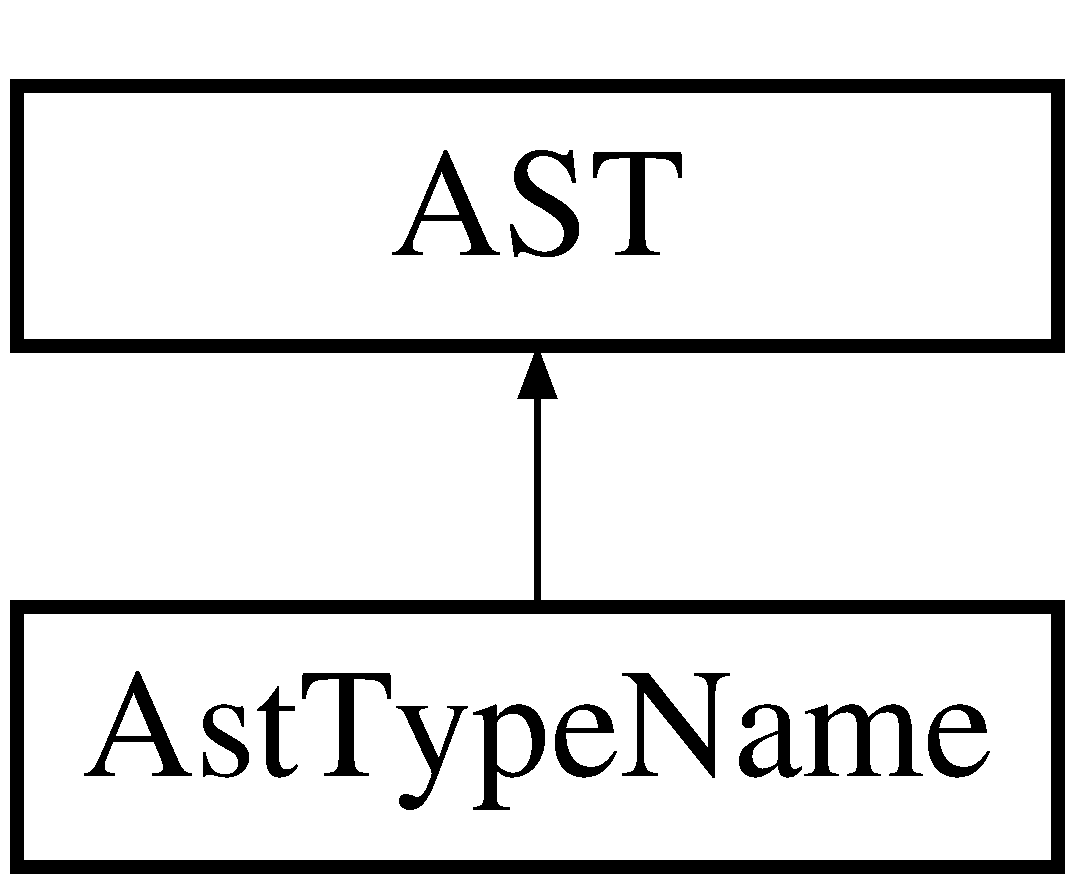
\includegraphics[height=2.000000cm]{classAstTypeName}
\end{center}
\end{figure}
\subsection*{Public Member Functions}
\begin{DoxyCompactItemize}
\item 
\hypertarget{classAstTypeName_aa60e9c67027276f2e082218aec5e8413}{{\bfseries Ast\-Type\-Name} (\hyperlink{classAstSpeciQualList}{Ast\-Speci\-Qual\-List} $\ast$list, \hyperlink{classAstAbstractDecl}{Ast\-Abstract\-Decl} $\ast$decl)}\label{classAstTypeName_aa60e9c67027276f2e082218aec5e8413}

\item 
void \hyperlink{classAstTypeName_adcd2b22b4135cadd7b9117e25a5dff45}{Visit} ()
\begin{DoxyCompactList}\small\item\em This function is responsible for tree traversals. \end{DoxyCompactList}\item 
\hypertarget{classAstTypeName_aa60e9c67027276f2e082218aec5e8413}{{\bfseries Ast\-Type\-Name} (\hyperlink{classAstSpeciQualList}{Ast\-Speci\-Qual\-List} $\ast$list, \hyperlink{classAstAbstractDecl}{Ast\-Abstract\-Decl} $\ast$decl)}\label{classAstTypeName_aa60e9c67027276f2e082218aec5e8413}

\item 
void \hyperlink{classAstTypeName_adcd2b22b4135cadd7b9117e25a5dff45}{Visit} ()
\begin{DoxyCompactList}\small\item\em This function is responsible for tree traversals. \end{DoxyCompactList}\item 
\hypertarget{classAstTypeName_aa60e9c67027276f2e082218aec5e8413}{{\bfseries Ast\-Type\-Name} (\hyperlink{classAstSpeciQualList}{Ast\-Speci\-Qual\-List} $\ast$list, \hyperlink{classAstAbstractDecl}{Ast\-Abstract\-Decl} $\ast$decl)}\label{classAstTypeName_aa60e9c67027276f2e082218aec5e8413}

\item 
void \hyperlink{classAstTypeName_adcd2b22b4135cadd7b9117e25a5dff45}{Visit} ()
\begin{DoxyCompactList}\small\item\em This function is responsible for tree traversals. \end{DoxyCompactList}\item 
\hypertarget{classAstTypeName_aa60e9c67027276f2e082218aec5e8413}{{\bfseries Ast\-Type\-Name} (\hyperlink{classAstSpeciQualList}{Ast\-Speci\-Qual\-List} $\ast$list, \hyperlink{classAstAbstractDecl}{Ast\-Abstract\-Decl} $\ast$decl)}\label{classAstTypeName_aa60e9c67027276f2e082218aec5e8413}

\item 
void \hyperlink{classAstTypeName_adcd2b22b4135cadd7b9117e25a5dff45}{Visit} ()
\begin{DoxyCompactList}\small\item\em This function is responsible for tree traversals. \end{DoxyCompactList}\item 
void \hyperlink{classAST_a71d680856e95ff89f55d5311a552eba6}{set\-Label} (string l)
\begin{DoxyCompactList}\small\item\em Sets the label for the node. \end{DoxyCompactList}\item 
void \hyperlink{classAST_a71d680856e95ff89f55d5311a552eba6}{set\-Label} (string l)
\begin{DoxyCompactList}\small\item\em Sets the label for the node. \end{DoxyCompactList}\item 
void \hyperlink{classAST_a71d680856e95ff89f55d5311a552eba6}{set\-Label} (string l)
\begin{DoxyCompactList}\small\item\em Sets the label for the node. \end{DoxyCompactList}\item 
void \hyperlink{classAST_a71d680856e95ff89f55d5311a552eba6}{set\-Label} (string l)
\begin{DoxyCompactList}\small\item\em Sets the label for the node. \end{DoxyCompactList}\item 
int \hyperlink{classAST_ab7a5b1d9f1c2de0d98deb356f724a42c}{get\-U\-I\-D} ()
\begin{DoxyCompactList}\small\item\em Gets the node's unique I\-D. \end{DoxyCompactList}\item 
int \hyperlink{classAST_ab7a5b1d9f1c2de0d98deb356f724a42c}{get\-U\-I\-D} ()
\begin{DoxyCompactList}\small\item\em Gets the node's unique I\-D. \end{DoxyCompactList}\item 
int \hyperlink{classAST_ab7a5b1d9f1c2de0d98deb356f724a42c}{get\-U\-I\-D} ()
\begin{DoxyCompactList}\small\item\em Gets the node's unique I\-D. \end{DoxyCompactList}\item 
int \hyperlink{classAST_ab7a5b1d9f1c2de0d98deb356f724a42c}{get\-U\-I\-D} ()
\begin{DoxyCompactList}\small\item\em Gets the node's unique I\-D. \end{DoxyCompactList}\item 
string \hyperlink{classAST_aee029be902fffc927d16ccb03eb922ad}{get\-Label} ()
\begin{DoxyCompactList}\small\item\em Gets the node's label. \end{DoxyCompactList}\item 
string \hyperlink{classAST_aee029be902fffc927d16ccb03eb922ad}{get\-Label} ()
\begin{DoxyCompactList}\small\item\em Gets the node's label. \end{DoxyCompactList}\item 
string \hyperlink{classAST_aee029be902fffc927d16ccb03eb922ad}{get\-Label} ()
\begin{DoxyCompactList}\small\item\em Gets the node's label. \end{DoxyCompactList}\item 
string \hyperlink{classAST_aee029be902fffc927d16ccb03eb922ad}{get\-Label} ()
\begin{DoxyCompactList}\small\item\em Gets the node's label. \end{DoxyCompactList}\end{DoxyCompactItemize}
\subsection*{Public Attributes}
\begin{DoxyCompactItemize}
\item 
\hypertarget{classAST_aaf215802de409f8096c063d01ffa6783}{bool \hyperlink{classAST_aaf215802de409f8096c063d01ffa6783}{needs\-Cast}}\label{classAST_aaf215802de409f8096c063d01ffa6783}

\begin{DoxyCompactList}\small\item\em This indicates if cast 3\-A\-C needs to be output, and is only relevant for expressions. \end{DoxyCompactList}\item 
\hypertarget{classAST_afa9e77ef650ec6664458fa6cb55be985}{bool \hyperlink{classAST_afa9e77ef650ec6664458fa6cb55be985}{is\-Conv}}\label{classAST_afa9e77ef650ec6664458fa6cb55be985}

\begin{DoxyCompactList}\small\item\em Indicates is a conversion is possible. \end{DoxyCompactList}\item 
\hypertarget{classAST_a61ef3317e023d45237e06615b387cd6b}{C\-O\-N\-V\-E\-R\-S\-I\-O\-N\-T\-Y\-P\-E \hyperlink{classAST_a61ef3317e023d45237e06615b387cd6b}{conv\-Type}}\label{classAST_a61ef3317e023d45237e06615b387cd6b}

\begin{DoxyCompactList}\small\item\em If needs\-Cast is true, then this indicates what the cast should be. \end{DoxyCompactList}\item 
\hypertarget{classAST_aea9b07b39d24183f38c0029cec0a878e}{int \hyperlink{classAST_aea9b07b39d24183f38c0029cec0a878e}{operand\-To\-Cast}}\label{classAST_aea9b07b39d24183f38c0029cec0a878e}

\begin{DoxyCompactList}\small\item\em This indicates if the first or second operand should be the one that is cast. \end{DoxyCompactList}\end{DoxyCompactItemize}
\subsection*{Static Public Attributes}
\begin{DoxyCompactItemize}
\item 
\hypertarget{classAST_a5fdfd5f7b104dd92889163bdadbc68d6}{static \hyperlink{classVisualizer}{Visualizer} \hyperlink{classAST_a5fdfd5f7b104dd92889163bdadbc68d6}{vis}}\label{classAST_a5fdfd5f7b104dd92889163bdadbc68d6}

\begin{DoxyCompactList}\small\item\em Static visualizer instance for generating the visualization of the \hyperlink{classAST}{A\-S\-T}. \end{DoxyCompactList}\item 
\hypertarget{classAST_a8a3ace322f50e030331065d644ee55ee}{static \hyperlink{classTAC__Generator}{T\-A\-C\-\_\-\-Generator} \hyperlink{classAST_a8a3ace322f50e030331065d644ee55ee}{tac\-Gen}}\label{classAST_a8a3ace322f50e030331065d644ee55ee}

\begin{DoxyCompactList}\small\item\em Three address code generator. \end{DoxyCompactList}\item 
\hypertarget{classAST_a1f69448c6dc368d005631a128460083d}{static string {\bfseries current\-Temp} =\char`\"{}\char`\"{}}\label{classAST_a1f69448c6dc368d005631a128460083d}

\item 
\hypertarget{classAST_a551aec090c932ab69365238b40a8a4eb}{static string \hyperlink{classAST_a551aec090c932ab69365238b40a8a4eb}{return\-Label} =\char`\"{}\char`\"{}}\label{classAST_a551aec090c932ab69365238b40a8a4eb}

\begin{DoxyCompactList}\small\item\em This is for storing the string id of any temporary result register that may be created during 3\-A\-C generation. \end{DoxyCompactList}\item 
\hypertarget{classAST_a73c0a266df52be71e6b527b6aa635173}{static list$<$ string $>$ {\bfseries temp\-Stack}}\label{classAST_a73c0a266df52be71e6b527b6aa635173}

\item 
\hypertarget{classAST_abf9e84b541ff04b7bb64e6e4371512d4}{static string {\bfseries last\-I\-D} =\char`\"{}\char`\"{}}\label{classAST_abf9e84b541ff04b7bb64e6e4371512d4}

\item 
\hypertarget{classAST_a163003bfe9c30510ec8039870346049f}{static \hyperlink{classSymTab}{Sym\-Tab} $\ast$ {\bfseries symbol\-Table} =N\-U\-L\-L}\label{classAST_a163003bfe9c30510ec8039870346049f}

\item 
\hypertarget{classAST_a5c3cc894d9c0453523dec9ed76f18a04}{static string {\bfseries current\-Function} =\char`\"{}\char`\"{}}\label{classAST_a5c3cc894d9c0453523dec9ed76f18a04}

\item 
\hypertarget{classAST_a66155513b59ff1a04c8ece8b20ec31f5}{static int {\bfseries current\-Constant\-Value} =0}\label{classAST_a66155513b59ff1a04c8ece8b20ec31f5}

\item 
\hypertarget{classAST_a3d031d7bab635ba1f015aade5943f40c}{static string {\bfseries current\-Id\-Name} =\char`\"{}\char`\"{}}\label{classAST_a3d031d7bab635ba1f015aade5943f40c}

\item 
\hypertarget{classAST_a16c4b6e54febc1a26b31a64a46972ef0}{static int {\bfseries current\-Index\-Val} = 0}\label{classAST_a16c4b6e54febc1a26b31a64a46972ef0}

\item 
\hypertarget{classAST_a6fc65ae9dd064a88941d4b88669b19db}{static string {\bfseries current\-I\-D} = \char`\"{}\char`\"{}}\label{classAST_a6fc65ae9dd064a88941d4b88669b19db}

\end{DoxyCompactItemize}
\subsection*{Protected Attributes}
\begin{DoxyCompactItemize}
\item 
\hypertarget{classAST_a847b778f1c3dd5a19de32de432ee6e15}{int \hyperlink{classAST_a847b778f1c3dd5a19de32de432ee6e15}{uid}}\label{classAST_a847b778f1c3dd5a19de32de432ee6e15}

\begin{DoxyCompactList}\small\item\em The unique id. \end{DoxyCompactList}\item 
\hypertarget{classAST_ab2e239ccc0688d2341724432ff5a1a31}{string \hyperlink{classAST_ab2e239ccc0688d2341724432ff5a1a31}{label}}\label{classAST_ab2e239ccc0688d2341724432ff5a1a31}

\begin{DoxyCompactList}\small\item\em The label to be printed in the visualization. \end{DoxyCompactList}\end{DoxyCompactItemize}
\subsection*{Private Attributes}
\begin{DoxyCompactItemize}
\item 
\hypertarget{classAstTypeName_a5cda7230ebcbdbff4a45799f4bc63ecf}{\hyperlink{classAstSpeciQualList}{Ast\-Speci\-Qual\-List} $\ast$ {\bfseries list}}\label{classAstTypeName_a5cda7230ebcbdbff4a45799f4bc63ecf}

\item 
\hypertarget{classAstTypeName_ae0f7104686f0c8856a053b198681acbd}{\hyperlink{classAstAbstractDecl}{Ast\-Abstract\-Decl} $\ast$ {\bfseries decl}}\label{classAstTypeName_ae0f7104686f0c8856a053b198681acbd}

\end{DoxyCompactItemize}


\subsection{Detailed Description}


Definition at line 104 of file Ast.\-h.



\subsection{Member Function Documentation}
\hypertarget{classAST_aee029be902fffc927d16ccb03eb922ad}{\index{Ast\-Type\-Name@{Ast\-Type\-Name}!get\-Label@{get\-Label}}
\index{get\-Label@{get\-Label}!AstTypeName@{Ast\-Type\-Name}}
\subsubsection[{get\-Label}]{\setlength{\rightskip}{0pt plus 5cm}string A\-S\-T\-::get\-Label (
\begin{DoxyParamCaption}
{}
\end{DoxyParamCaption}
)\hspace{0.3cm}{\ttfamily [inline]}, {\ttfamily [inherited]}}}\label{classAST_aee029be902fffc927d16ccb03eb922ad}


Gets the node's label. 

\begin{DoxyReturn}{Returns}
The label 
\end{DoxyReturn}


Definition at line 60 of file Ast.\-h.

\hypertarget{classAST_aee029be902fffc927d16ccb03eb922ad}{\index{Ast\-Type\-Name@{Ast\-Type\-Name}!get\-Label@{get\-Label}}
\index{get\-Label@{get\-Label}!AstTypeName@{Ast\-Type\-Name}}
\subsubsection[{get\-Label}]{\setlength{\rightskip}{0pt plus 5cm}string A\-S\-T\-::get\-Label (
\begin{DoxyParamCaption}
{}
\end{DoxyParamCaption}
)\hspace{0.3cm}{\ttfamily [inline]}, {\ttfamily [inherited]}}}\label{classAST_aee029be902fffc927d16ccb03eb922ad}


Gets the node's label. 

\begin{DoxyReturn}{Returns}
The label 
\end{DoxyReturn}


Definition at line 60 of file C\-Scanner.\-ll.

\hypertarget{classAST_aee029be902fffc927d16ccb03eb922ad}{\index{Ast\-Type\-Name@{Ast\-Type\-Name}!get\-Label@{get\-Label}}
\index{get\-Label@{get\-Label}!AstTypeName@{Ast\-Type\-Name}}
\subsubsection[{get\-Label}]{\setlength{\rightskip}{0pt plus 5cm}string A\-S\-T\-::get\-Label (
\begin{DoxyParamCaption}
{}
\end{DoxyParamCaption}
)\hspace{0.3cm}{\ttfamily [inline]}, {\ttfamily [inherited]}}}\label{classAST_aee029be902fffc927d16ccb03eb922ad}


Gets the node's label. 

\begin{DoxyReturn}{Returns}
The label 
\end{DoxyReturn}


Definition at line 60 of file C\-Parser.\-yy.

\hypertarget{classAST_aee029be902fffc927d16ccb03eb922ad}{\index{Ast\-Type\-Name@{Ast\-Type\-Name}!get\-Label@{get\-Label}}
\index{get\-Label@{get\-Label}!AstTypeName@{Ast\-Type\-Name}}
\subsubsection[{get\-Label}]{\setlength{\rightskip}{0pt plus 5cm}string A\-S\-T\-::get\-Label (
\begin{DoxyParamCaption}
{}
\end{DoxyParamCaption}
)\hspace{0.3cm}{\ttfamily [inline]}, {\ttfamily [inherited]}}}\label{classAST_aee029be902fffc927d16ccb03eb922ad}


Gets the node's label. 

\begin{DoxyReturn}{Returns}
The label 
\end{DoxyReturn}


Definition at line 60 of file C\-Parser.\-yy.

\hypertarget{classAST_ab7a5b1d9f1c2de0d98deb356f724a42c}{\index{Ast\-Type\-Name@{Ast\-Type\-Name}!get\-U\-I\-D@{get\-U\-I\-D}}
\index{get\-U\-I\-D@{get\-U\-I\-D}!AstTypeName@{Ast\-Type\-Name}}
\subsubsection[{get\-U\-I\-D}]{\setlength{\rightskip}{0pt plus 5cm}int A\-S\-T\-::get\-U\-I\-D (
\begin{DoxyParamCaption}
{}
\end{DoxyParamCaption}
)\hspace{0.3cm}{\ttfamily [inline]}, {\ttfamily [inherited]}}}\label{classAST_ab7a5b1d9f1c2de0d98deb356f724a42c}


Gets the node's unique I\-D. 

\begin{DoxyReturn}{Returns}
The unique id 
\end{DoxyReturn}


Definition at line 53 of file C\-Parser.\-yy.

\hypertarget{classAST_ab7a5b1d9f1c2de0d98deb356f724a42c}{\index{Ast\-Type\-Name@{Ast\-Type\-Name}!get\-U\-I\-D@{get\-U\-I\-D}}
\index{get\-U\-I\-D@{get\-U\-I\-D}!AstTypeName@{Ast\-Type\-Name}}
\subsubsection[{get\-U\-I\-D}]{\setlength{\rightskip}{0pt plus 5cm}int A\-S\-T\-::get\-U\-I\-D (
\begin{DoxyParamCaption}
{}
\end{DoxyParamCaption}
)\hspace{0.3cm}{\ttfamily [inline]}, {\ttfamily [inherited]}}}\label{classAST_ab7a5b1d9f1c2de0d98deb356f724a42c}


Gets the node's unique I\-D. 

\begin{DoxyReturn}{Returns}
The unique id 
\end{DoxyReturn}


Definition at line 53 of file C\-Parser.\-yy.

\hypertarget{classAST_ab7a5b1d9f1c2de0d98deb356f724a42c}{\index{Ast\-Type\-Name@{Ast\-Type\-Name}!get\-U\-I\-D@{get\-U\-I\-D}}
\index{get\-U\-I\-D@{get\-U\-I\-D}!AstTypeName@{Ast\-Type\-Name}}
\subsubsection[{get\-U\-I\-D}]{\setlength{\rightskip}{0pt plus 5cm}int A\-S\-T\-::get\-U\-I\-D (
\begin{DoxyParamCaption}
{}
\end{DoxyParamCaption}
)\hspace{0.3cm}{\ttfamily [inline]}, {\ttfamily [inherited]}}}\label{classAST_ab7a5b1d9f1c2de0d98deb356f724a42c}


Gets the node's unique I\-D. 

\begin{DoxyReturn}{Returns}
The unique id 
\end{DoxyReturn}


Definition at line 53 of file C\-Scanner.\-ll.

\hypertarget{classAST_ab7a5b1d9f1c2de0d98deb356f724a42c}{\index{Ast\-Type\-Name@{Ast\-Type\-Name}!get\-U\-I\-D@{get\-U\-I\-D}}
\index{get\-U\-I\-D@{get\-U\-I\-D}!AstTypeName@{Ast\-Type\-Name}}
\subsubsection[{get\-U\-I\-D}]{\setlength{\rightskip}{0pt plus 5cm}int A\-S\-T\-::get\-U\-I\-D (
\begin{DoxyParamCaption}
{}
\end{DoxyParamCaption}
)\hspace{0.3cm}{\ttfamily [inline]}, {\ttfamily [inherited]}}}\label{classAST_ab7a5b1d9f1c2de0d98deb356f724a42c}


Gets the node's unique I\-D. 

\begin{DoxyReturn}{Returns}
The unique id 
\end{DoxyReturn}


Definition at line 53 of file Ast.\-h.

\hypertarget{classAST_a71d680856e95ff89f55d5311a552eba6}{\index{Ast\-Type\-Name@{Ast\-Type\-Name}!set\-Label@{set\-Label}}
\index{set\-Label@{set\-Label}!AstTypeName@{Ast\-Type\-Name}}
\subsubsection[{set\-Label}]{\setlength{\rightskip}{0pt plus 5cm}void A\-S\-T\-::set\-Label (
\begin{DoxyParamCaption}
\item[{string}]{l}
\end{DoxyParamCaption}
)\hspace{0.3cm}{\ttfamily [inline]}, {\ttfamily [inherited]}}}\label{classAST_a71d680856e95ff89f55d5311a552eba6}


Sets the label for the node. 


\begin{DoxyParams}{Parameters}
{\em l} & The label string \\
\hline
\end{DoxyParams}


Definition at line 43 of file C\-Scanner.\-ll.

\hypertarget{classAST_a71d680856e95ff89f55d5311a552eba6}{\index{Ast\-Type\-Name@{Ast\-Type\-Name}!set\-Label@{set\-Label}}
\index{set\-Label@{set\-Label}!AstTypeName@{Ast\-Type\-Name}}
\subsubsection[{set\-Label}]{\setlength{\rightskip}{0pt plus 5cm}void A\-S\-T\-::set\-Label (
\begin{DoxyParamCaption}
\item[{string}]{l}
\end{DoxyParamCaption}
)\hspace{0.3cm}{\ttfamily [inline]}, {\ttfamily [inherited]}}}\label{classAST_a71d680856e95ff89f55d5311a552eba6}


Sets the label for the node. 


\begin{DoxyParams}{Parameters}
{\em l} & The label string \\
\hline
\end{DoxyParams}


Definition at line 43 of file C\-Parser.\-yy.

\hypertarget{classAST_a71d680856e95ff89f55d5311a552eba6}{\index{Ast\-Type\-Name@{Ast\-Type\-Name}!set\-Label@{set\-Label}}
\index{set\-Label@{set\-Label}!AstTypeName@{Ast\-Type\-Name}}
\subsubsection[{set\-Label}]{\setlength{\rightskip}{0pt plus 5cm}void A\-S\-T\-::set\-Label (
\begin{DoxyParamCaption}
\item[{string}]{l}
\end{DoxyParamCaption}
)\hspace{0.3cm}{\ttfamily [inline]}, {\ttfamily [inherited]}}}\label{classAST_a71d680856e95ff89f55d5311a552eba6}


Sets the label for the node. 


\begin{DoxyParams}{Parameters}
{\em l} & The label string \\
\hline
\end{DoxyParams}


Definition at line 43 of file Ast.\-h.

\hypertarget{classAST_a71d680856e95ff89f55d5311a552eba6}{\index{Ast\-Type\-Name@{Ast\-Type\-Name}!set\-Label@{set\-Label}}
\index{set\-Label@{set\-Label}!AstTypeName@{Ast\-Type\-Name}}
\subsubsection[{set\-Label}]{\setlength{\rightskip}{0pt plus 5cm}void A\-S\-T\-::set\-Label (
\begin{DoxyParamCaption}
\item[{string}]{l}
\end{DoxyParamCaption}
)\hspace{0.3cm}{\ttfamily [inline]}, {\ttfamily [inherited]}}}\label{classAST_a71d680856e95ff89f55d5311a552eba6}


Sets the label for the node. 


\begin{DoxyParams}{Parameters}
{\em l} & The label string \\
\hline
\end{DoxyParams}


Definition at line 43 of file C\-Parser.\-yy.

\hypertarget{classAstTypeName_adcd2b22b4135cadd7b9117e25a5dff45}{\index{Ast\-Type\-Name@{Ast\-Type\-Name}!Visit@{Visit}}
\index{Visit@{Visit}!AstTypeName@{Ast\-Type\-Name}}
\subsubsection[{Visit}]{\setlength{\rightskip}{0pt plus 5cm}void Ast\-Type\-Name\-::\-Visit (
\begin{DoxyParamCaption}
{}
\end{DoxyParamCaption}
)\hspace{0.3cm}{\ttfamily [virtual]}}}\label{classAstTypeName_adcd2b22b4135cadd7b9117e25a5dff45}


This function is responsible for tree traversals. 

This function will call the Visit functions of each of it's children nodes, call the visualization code for itself, and output any 3\-A\-C that can be generated at the current node. 

Reimplemented from \hyperlink{classAST_a5828cc86f2c4f1a0aeab6d7069e8fd82}{A\-S\-T}.



Definition at line 867 of file Ast.\-cpp.

\hypertarget{classAstTypeName_adcd2b22b4135cadd7b9117e25a5dff45}{\index{Ast\-Type\-Name@{Ast\-Type\-Name}!Visit@{Visit}}
\index{Visit@{Visit}!AstTypeName@{Ast\-Type\-Name}}
\subsubsection[{Visit}]{\setlength{\rightskip}{0pt plus 5cm}void Ast\-Type\-Name\-::\-Visit (
\begin{DoxyParamCaption}
{}
\end{DoxyParamCaption}
)\hspace{0.3cm}{\ttfamily [virtual]}}}\label{classAstTypeName_adcd2b22b4135cadd7b9117e25a5dff45}


This function is responsible for tree traversals. 

This function will call the Visit functions of each of it's children nodes, call the visualization code for itself, and output any 3\-A\-C that can be generated at the current node. 

Reimplemented from \hyperlink{classAST_a5828cc86f2c4f1a0aeab6d7069e8fd82}{A\-S\-T}.

\hypertarget{classAstTypeName_adcd2b22b4135cadd7b9117e25a5dff45}{\index{Ast\-Type\-Name@{Ast\-Type\-Name}!Visit@{Visit}}
\index{Visit@{Visit}!AstTypeName@{Ast\-Type\-Name}}
\subsubsection[{Visit}]{\setlength{\rightskip}{0pt plus 5cm}void Ast\-Type\-Name\-::\-Visit (
\begin{DoxyParamCaption}
{}
\end{DoxyParamCaption}
)\hspace{0.3cm}{\ttfamily [virtual]}}}\label{classAstTypeName_adcd2b22b4135cadd7b9117e25a5dff45}


This function is responsible for tree traversals. 

This function will call the Visit functions of each of it's children nodes, call the visualization code for itself, and output any 3\-A\-C that can be generated at the current node. 

Reimplemented from \hyperlink{classAST_a5828cc86f2c4f1a0aeab6d7069e8fd82}{A\-S\-T}.

\hypertarget{classAstTypeName_adcd2b22b4135cadd7b9117e25a5dff45}{\index{Ast\-Type\-Name@{Ast\-Type\-Name}!Visit@{Visit}}
\index{Visit@{Visit}!AstTypeName@{Ast\-Type\-Name}}
\subsubsection[{Visit}]{\setlength{\rightskip}{0pt plus 5cm}void Ast\-Type\-Name\-::\-Visit (
\begin{DoxyParamCaption}
{}
\end{DoxyParamCaption}
)\hspace{0.3cm}{\ttfamily [virtual]}}}\label{classAstTypeName_adcd2b22b4135cadd7b9117e25a5dff45}


This function is responsible for tree traversals. 

This function will call the Visit functions of each of it's children nodes, call the visualization code for itself, and output any 3\-A\-C that can be generated at the current node. 

Reimplemented from \hyperlink{classAST_a5828cc86f2c4f1a0aeab6d7069e8fd82}{A\-S\-T}.



The documentation for this class was generated from the following files\-:\begin{DoxyCompactItemize}
\item 
Ast.\-h\item 
Ast.\-cpp\end{DoxyCompactItemize}

\input{classAstTypeParamList}
\input{classAstTypeQualList}
\input{classAstTypeSpeci}
\hypertarget{classAstUnaryExpr}{\section{Ast\-Unary\-Expr Class Reference}
\label{classAstUnaryExpr}\index{Ast\-Unary\-Expr@{Ast\-Unary\-Expr}}
}
Inheritance diagram for Ast\-Unary\-Expr\-:\begin{figure}[H]
\begin{center}
\leavevmode
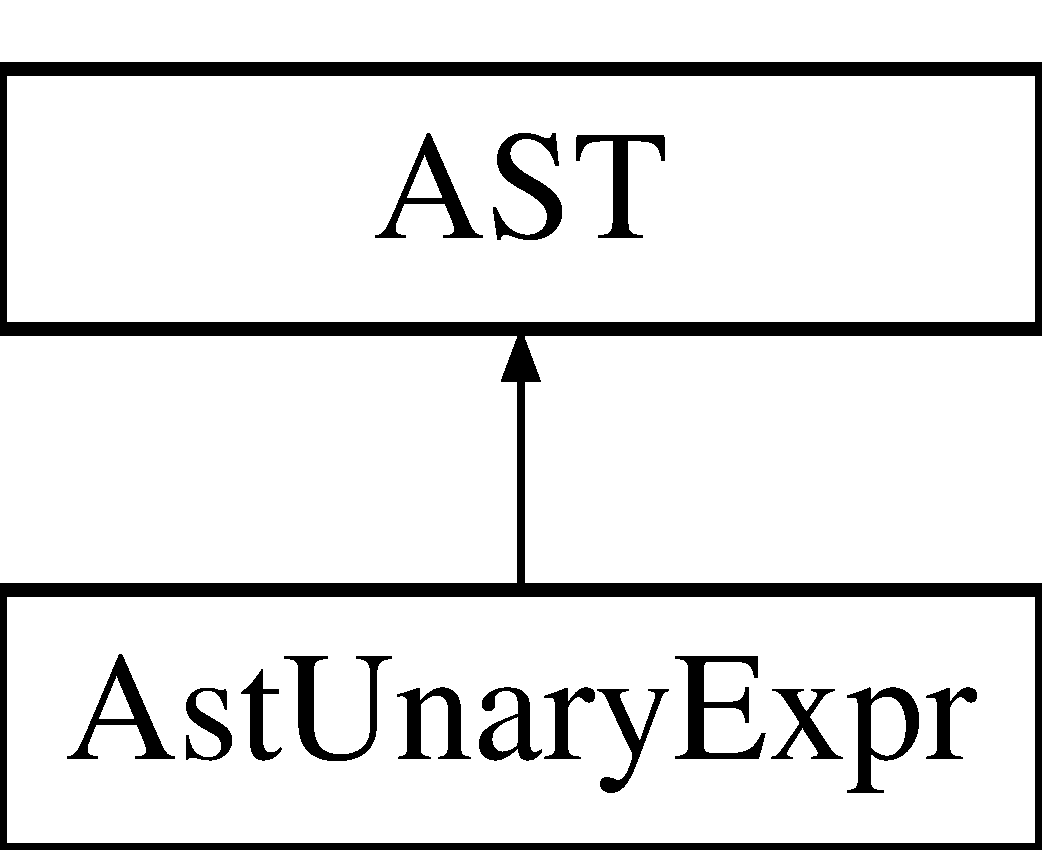
\includegraphics[height=2.000000cm]{classAstUnaryExpr}
\end{center}
\end{figure}
\subsection*{Public Types}
\begin{DoxyCompactItemize}
\item 
enum {\bfseries Type} \{ \\*
{\bfseries P\-O\-S\-T\-F\-I\-X}, 
{\bfseries I\-N\-C}, 
{\bfseries D\-E\-C}, 
{\bfseries C\-A\-S\-T}, 
\\*
{\bfseries S\-I\-Z\-E\-O\-F}, 
{\bfseries S\-I\-Z\-E\-O\-F\-\_\-\-T\-Y\-P\-E}
 \}
\end{DoxyCompactItemize}
\subsection*{Public Member Functions}
\begin{DoxyCompactItemize}
\item 
\hypertarget{classAstUnaryExpr_a7afc6e7c4cf309676aa701656c70453a}{{\bfseries Ast\-Unary\-Expr} (\hyperlink{classAstPostfixExpr}{Ast\-Postfix\-Expr} $\ast$e)}\label{classAstUnaryExpr_a7afc6e7c4cf309676aa701656c70453a}

\item 
\hypertarget{classAstUnaryExpr_a82859566c71d787e29263ff3ba013261}{{\bfseries Ast\-Unary\-Expr} (\hyperlink{classAstUnaryExpr}{Ast\-Unary\-Expr} $\ast$e, bool inc)}\label{classAstUnaryExpr_a82859566c71d787e29263ff3ba013261}

\item 
\hypertarget{classAstUnaryExpr_ad71de2cd2c65b31e5f5f5fde4e75fc14}{{\bfseries Ast\-Unary\-Expr} (\hyperlink{classAstUnaryOp}{Ast\-Unary\-Op} $\ast$o, \hyperlink{classAstCastExpr}{Ast\-Cast\-Expr} $\ast$c)}\label{classAstUnaryExpr_ad71de2cd2c65b31e5f5f5fde4e75fc14}

\item 
\hypertarget{classAstUnaryExpr_a22b7c004d42c54c96b40de10cc90a07e}{{\bfseries Ast\-Unary\-Expr} (\hyperlink{classAstUnaryExpr}{Ast\-Unary\-Expr} $\ast$e)}\label{classAstUnaryExpr_a22b7c004d42c54c96b40de10cc90a07e}

\item 
\hypertarget{classAstUnaryExpr_a305b745cf1449c3d3dc4e74dcd768ef1}{{\bfseries Ast\-Unary\-Expr} (\hyperlink{classAstTypeName}{Ast\-Type\-Name} $\ast$t)}\label{classAstUnaryExpr_a305b745cf1449c3d3dc4e74dcd768ef1}

\item 
void \hyperlink{classAstUnaryExpr_ae35427088d6f5c889e8e80573a3750fc}{Visit} ()
\begin{DoxyCompactList}\small\item\em This function is responsible for tree traversals. \end{DoxyCompactList}\item 
void \hyperlink{classAST_a71d680856e95ff89f55d5311a552eba6}{set\-Label} (string l)
\begin{DoxyCompactList}\small\item\em Sets the label for the node. \end{DoxyCompactList}\item 
int \hyperlink{classAST_ab7a5b1d9f1c2de0d98deb356f724a42c}{get\-U\-I\-D} ()
\begin{DoxyCompactList}\small\item\em Gets the node's unique I\-D. \end{DoxyCompactList}\item 
string \hyperlink{classAST_aee029be902fffc927d16ccb03eb922ad}{get\-Label} ()
\begin{DoxyCompactList}\small\item\em Gets the node's label. \end{DoxyCompactList}\end{DoxyCompactItemize}
\subsection*{Public Attributes}
\begin{DoxyCompactItemize}
\item 
\hypertarget{classAstUnaryExpr_aa3cec070038e9d68b11137b18aeb478f}{enum Ast\-Unary\-Expr\-::\-Type {\bfseries t}}\label{classAstUnaryExpr_aa3cec070038e9d68b11137b18aeb478f}

\end{DoxyCompactItemize}
\subsection*{Static Public Attributes}
\begin{DoxyCompactItemize}
\item 
\hypertarget{classAST_aca9e6637209b31e03a09c0d42f29bdfa}{static \hyperlink{classVisualizer}{Visualizer} \hyperlink{classAST_aca9e6637209b31e03a09c0d42f29bdfa}{vis}}\label{classAST_aca9e6637209b31e03a09c0d42f29bdfa}

\begin{DoxyCompactList}\small\item\em Static visualizer instance for generating the visualization of the \hyperlink{classAST}{A\-S\-T}. \end{DoxyCompactList}\end{DoxyCompactItemize}
\subsection*{Protected Attributes}
\begin{DoxyCompactItemize}
\item 
\hypertarget{classAST_a847b778f1c3dd5a19de32de432ee6e15}{int \hyperlink{classAST_a847b778f1c3dd5a19de32de432ee6e15}{uid}}\label{classAST_a847b778f1c3dd5a19de32de432ee6e15}

\begin{DoxyCompactList}\small\item\em The unique id. \end{DoxyCompactList}\item 
\hypertarget{classAST_ab2e239ccc0688d2341724432ff5a1a31}{string \hyperlink{classAST_ab2e239ccc0688d2341724432ff5a1a31}{label}}\label{classAST_ab2e239ccc0688d2341724432ff5a1a31}

\begin{DoxyCompactList}\small\item\em The label to be printed in the visualization. \end{DoxyCompactList}\end{DoxyCompactItemize}
\subsection*{Private Attributes}
\begin{DoxyCompactItemize}
\item 
\hypertarget{classAstUnaryExpr_a390969e72a1daaf0a5aff4e59d29a851}{\hyperlink{classAstPostfixExpr}{Ast\-Postfix\-Expr} $\ast$ {\bfseries expr}}\label{classAstUnaryExpr_a390969e72a1daaf0a5aff4e59d29a851}

\item 
\hypertarget{classAstUnaryExpr_a76418e6a58878a1da236456a7e232168}{bool {\bfseries is\-I\-N\-C}}\label{classAstUnaryExpr_a76418e6a58878a1da236456a7e232168}

\item 
\hypertarget{classAstUnaryExpr_af5b5ac5242011e11a12a6697812ec459}{bool {\bfseries is\-D\-E\-C}}\label{classAstUnaryExpr_af5b5ac5242011e11a12a6697812ec459}

\item 
\hypertarget{classAstUnaryExpr_a1d3690f3309ab7f577bfb0ac9ac71a1e}{\hyperlink{classAstUnaryOp}{Ast\-Unary\-Op} $\ast$ {\bfseries op}}\label{classAstUnaryExpr_a1d3690f3309ab7f577bfb0ac9ac71a1e}

\item 
\hypertarget{classAstUnaryExpr_a294141f6ff7096b852811c9255d8da28}{\hyperlink{classAstCastExpr}{Ast\-Cast\-Expr} $\ast$ {\bfseries cast}}\label{classAstUnaryExpr_a294141f6ff7096b852811c9255d8da28}

\item 
\hypertarget{classAstUnaryExpr_a1a6ec44fa3bb94d0aa4743be89350d06}{\hyperlink{classAstUnaryExpr}{Ast\-Unary\-Expr} $\ast$ {\bfseries uniexpr}}\label{classAstUnaryExpr_a1a6ec44fa3bb94d0aa4743be89350d06}

\item 
\hypertarget{classAstUnaryExpr_a9c87556bbc6caa12e41760e01d9035e6}{\hyperlink{classAstTypeName}{Ast\-Type\-Name} $\ast$ {\bfseries tname}}\label{classAstUnaryExpr_a9c87556bbc6caa12e41760e01d9035e6}

\end{DoxyCompactItemize}


\subsection{Member Function Documentation}
\hypertarget{classAST_aee029be902fffc927d16ccb03eb922ad}{\index{Ast\-Unary\-Expr@{Ast\-Unary\-Expr}!get\-Label@{get\-Label}}
\index{get\-Label@{get\-Label}!AstUnaryExpr@{Ast\-Unary\-Expr}}
\subsubsection[{get\-Label}]{\setlength{\rightskip}{0pt plus 5cm}string A\-S\-T\-::get\-Label (
\begin{DoxyParamCaption}
{}
\end{DoxyParamCaption}
)\hspace{0.3cm}{\ttfamily [inline]}, {\ttfamily [inherited]}}}\label{classAST_aee029be902fffc927d16ccb03eb922ad}


Gets the node's label. 

\begin{DoxyReturn}{Returns}
The label 
\end{DoxyReturn}
\hypertarget{classAST_ab7a5b1d9f1c2de0d98deb356f724a42c}{\index{Ast\-Unary\-Expr@{Ast\-Unary\-Expr}!get\-U\-I\-D@{get\-U\-I\-D}}
\index{get\-U\-I\-D@{get\-U\-I\-D}!AstUnaryExpr@{Ast\-Unary\-Expr}}
\subsubsection[{get\-U\-I\-D}]{\setlength{\rightskip}{0pt plus 5cm}int A\-S\-T\-::get\-U\-I\-D (
\begin{DoxyParamCaption}
{}
\end{DoxyParamCaption}
)\hspace{0.3cm}{\ttfamily [inline]}, {\ttfamily [inherited]}}}\label{classAST_ab7a5b1d9f1c2de0d98deb356f724a42c}


Gets the node's unique I\-D. 

\begin{DoxyReturn}{Returns}
The unique id 
\end{DoxyReturn}
\hypertarget{classAST_a71d680856e95ff89f55d5311a552eba6}{\index{Ast\-Unary\-Expr@{Ast\-Unary\-Expr}!set\-Label@{set\-Label}}
\index{set\-Label@{set\-Label}!AstUnaryExpr@{Ast\-Unary\-Expr}}
\subsubsection[{set\-Label}]{\setlength{\rightskip}{0pt plus 5cm}void A\-S\-T\-::set\-Label (
\begin{DoxyParamCaption}
\item[{string}]{l}
\end{DoxyParamCaption}
)\hspace{0.3cm}{\ttfamily [inline]}, {\ttfamily [inherited]}}}\label{classAST_a71d680856e95ff89f55d5311a552eba6}


Sets the label for the node. 


\begin{DoxyParams}{Parameters}
{\em l} & The label string \\
\hline
\end{DoxyParams}
\hypertarget{classAstUnaryExpr_ae35427088d6f5c889e8e80573a3750fc}{\index{Ast\-Unary\-Expr@{Ast\-Unary\-Expr}!Visit@{Visit}}
\index{Visit@{Visit}!AstUnaryExpr@{Ast\-Unary\-Expr}}
\subsubsection[{Visit}]{\setlength{\rightskip}{0pt plus 5cm}void Ast\-Unary\-Expr\-::\-Visit (
\begin{DoxyParamCaption}
{}
\end{DoxyParamCaption}
)\hspace{0.3cm}{\ttfamily [virtual]}}}\label{classAstUnaryExpr_ae35427088d6f5c889e8e80573a3750fc}


This function is responsible for tree traversals. 

This function will call the Visit functions of each of it's children nodes, call the visualization code for itself, and output any 3\-A\-C that can be generated at the current node. 

Reimplemented from \hyperlink{classAST_a5828cc86f2c4f1a0aeab6d7069e8fd82}{A\-S\-T}.



The documentation for this class was generated from the following files\-:\begin{DoxyCompactItemize}
\item 
Ast.\-h\item 
Ast.\-cpp\end{DoxyCompactItemize}

\hypertarget{classAstUnaryOp}{\section{Ast\-Unary\-Op Class Reference}
\label{classAstUnaryOp}\index{Ast\-Unary\-Op@{Ast\-Unary\-Op}}
}
Inheritance diagram for Ast\-Unary\-Op\-:\begin{figure}[H]
\begin{center}
\leavevmode
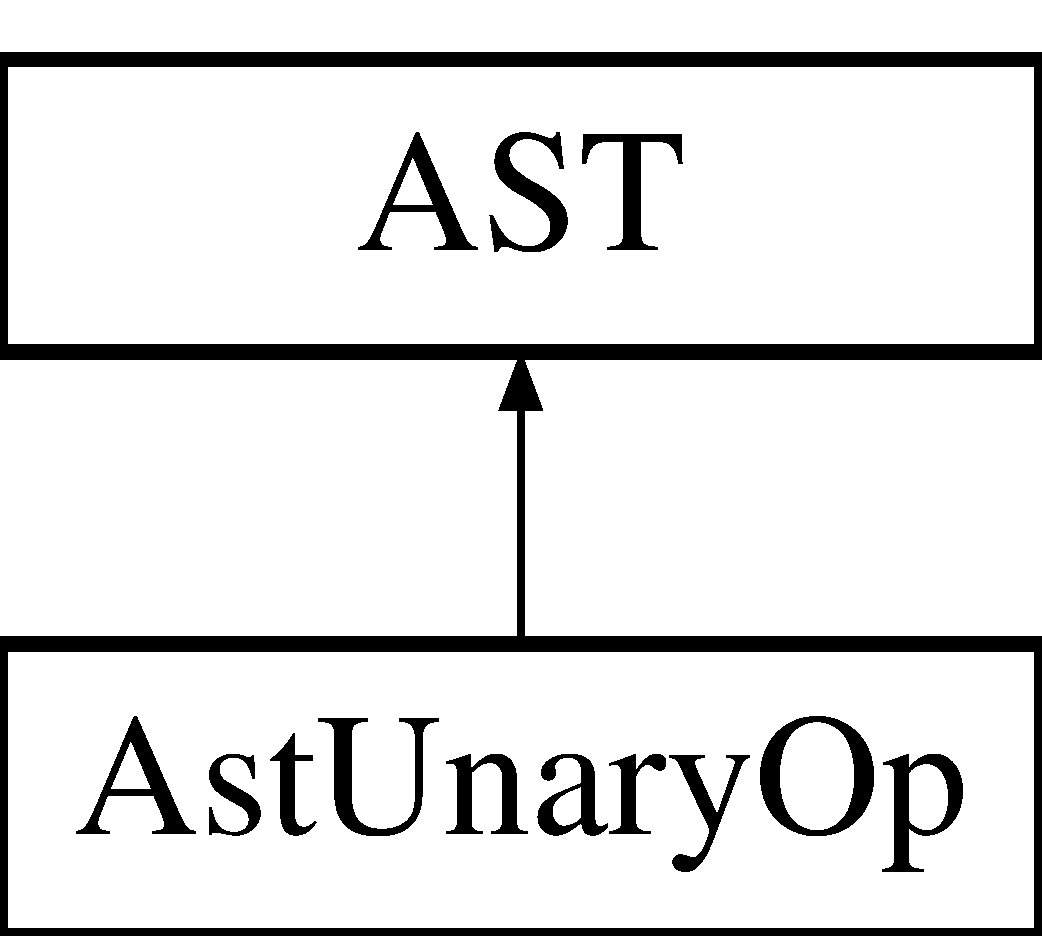
\includegraphics[height=2.000000cm]{classAstUnaryOp}
\end{center}
\end{figure}
\subsection*{Public Types}
\begin{DoxyCompactItemize}
\item 
enum {\bfseries Operator} \{ \\*
{\bfseries B\-I\-N\-\_\-\-A\-N\-D}, 
{\bfseries S\-T\-A\-R}, 
{\bfseries P\-L\-U\-S}, 
{\bfseries M\-I\-N\-U\-S}, 
\\*
{\bfseries T\-I\-L\-D\-E}, 
{\bfseries B\-A\-N\-G}
 \}
\end{DoxyCompactItemize}
\subsection*{Public Member Functions}
\begin{DoxyCompactItemize}
\item 
\hypertarget{classAstUnaryOp_aa363b2df2fbb4653a683899e59df2080}{{\bfseries Ast\-Unary\-Op} (Operator o)}\label{classAstUnaryOp_aa363b2df2fbb4653a683899e59df2080}

\item 
\hypertarget{classAstUnaryOp_a23e13d42f33d5882d58ca48e8053f1a0}{void {\bfseries Visit} ()}\label{classAstUnaryOp_a23e13d42f33d5882d58ca48e8053f1a0}

\item 
\hypertarget{classAST_a71d680856e95ff89f55d5311a552eba6}{void {\bfseries set\-Label} (string l)}\label{classAST_a71d680856e95ff89f55d5311a552eba6}

\item 
\hypertarget{classAST_ab7a5b1d9f1c2de0d98deb356f724a42c}{int {\bfseries get\-U\-I\-D} ()}\label{classAST_ab7a5b1d9f1c2de0d98deb356f724a42c}

\item 
\hypertarget{classAST_aee029be902fffc927d16ccb03eb922ad}{string {\bfseries get\-Label} ()}\label{classAST_aee029be902fffc927d16ccb03eb922ad}

\end{DoxyCompactItemize}
\subsection*{Static Public Attributes}
\begin{DoxyCompactItemize}
\item 
\hypertarget{classAST_aca9e6637209b31e03a09c0d42f29bdfa}{static \hyperlink{classVisualizer}{Visualizer} {\bfseries vis}}\label{classAST_aca9e6637209b31e03a09c0d42f29bdfa}

\end{DoxyCompactItemize}
\subsection*{Protected Attributes}
\begin{DoxyCompactItemize}
\item 
\hypertarget{classAST_a847b778f1c3dd5a19de32de432ee6e15}{int {\bfseries uid}}\label{classAST_a847b778f1c3dd5a19de32de432ee6e15}

\item 
\hypertarget{classAST_ab2e239ccc0688d2341724432ff5a1a31}{string {\bfseries label}}\label{classAST_ab2e239ccc0688d2341724432ff5a1a31}

\end{DoxyCompactItemize}
\subsection*{Private Attributes}
\begin{DoxyCompactItemize}
\item 
\hypertarget{classAstUnaryOp_af64ad21f350c4f1a4cfc24c6bc5e992a}{Operator {\bfseries op}}\label{classAstUnaryOp_af64ad21f350c4f1a4cfc24c6bc5e992a}

\end{DoxyCompactItemize}


The documentation for this class was generated from the following files\-:\begin{DoxyCompactItemize}
\item 
Ast.\-h\item 
Ast.\-cpp\end{DoxyCompactItemize}

\hypertarget{classAstWhile}{\section{Ast\-While Class Reference}
\label{classAstWhile}\index{Ast\-While@{Ast\-While}}
}
Inheritance diagram for Ast\-While\-:\begin{figure}[H]
\begin{center}
\leavevmode
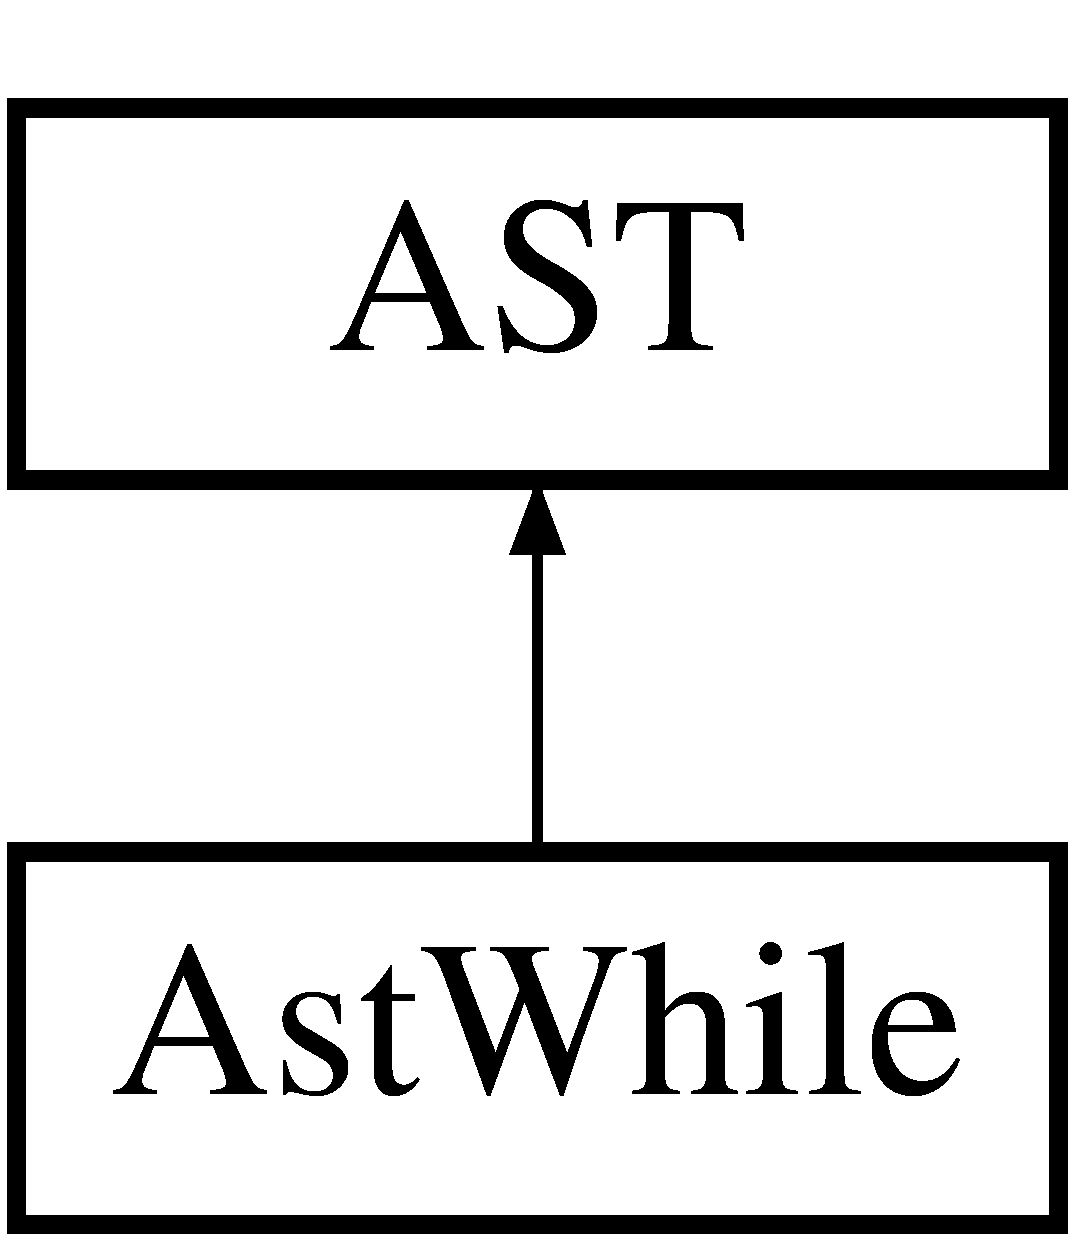
\includegraphics[height=2.000000cm]{classAstWhile}
\end{center}
\end{figure}
\subsection*{Public Member Functions}
\begin{DoxyCompactItemize}
\item 
\hypertarget{classAstWhile_a4c0e68b002b9425fba3f3e7b21a31e64}{{\bfseries Ast\-While} (\hyperlink{classAstExpression}{Ast\-Expression} $\ast$test, \hyperlink{classAstStatement}{Ast\-Statement} $\ast$statement)}\label{classAstWhile_a4c0e68b002b9425fba3f3e7b21a31e64}

\item 
void \hyperlink{classAstWhile_a9bf8eb5f0f63a4f0dc7b7201f292d4dd}{Visit} ()
\begin{DoxyCompactList}\small\item\em This function is responsible for tree traversals. \end{DoxyCompactList}\item 
\hypertarget{classAstWhile_a4c0e68b002b9425fba3f3e7b21a31e64}{{\bfseries Ast\-While} (\hyperlink{classAstExpression}{Ast\-Expression} $\ast$test, \hyperlink{classAstStatement}{Ast\-Statement} $\ast$statement)}\label{classAstWhile_a4c0e68b002b9425fba3f3e7b21a31e64}

\item 
void \hyperlink{classAstWhile_a9bf8eb5f0f63a4f0dc7b7201f292d4dd}{Visit} ()
\begin{DoxyCompactList}\small\item\em This function is responsible for tree traversals. \end{DoxyCompactList}\item 
\hypertarget{classAstWhile_a4c0e68b002b9425fba3f3e7b21a31e64}{{\bfseries Ast\-While} (\hyperlink{classAstExpression}{Ast\-Expression} $\ast$test, \hyperlink{classAstStatement}{Ast\-Statement} $\ast$statement)}\label{classAstWhile_a4c0e68b002b9425fba3f3e7b21a31e64}

\item 
void \hyperlink{classAstWhile_a9bf8eb5f0f63a4f0dc7b7201f292d4dd}{Visit} ()
\begin{DoxyCompactList}\small\item\em This function is responsible for tree traversals. \end{DoxyCompactList}\item 
\hypertarget{classAstWhile_a4c0e68b002b9425fba3f3e7b21a31e64}{{\bfseries Ast\-While} (\hyperlink{classAstExpression}{Ast\-Expression} $\ast$test, \hyperlink{classAstStatement}{Ast\-Statement} $\ast$statement)}\label{classAstWhile_a4c0e68b002b9425fba3f3e7b21a31e64}

\item 
void \hyperlink{classAstWhile_a9bf8eb5f0f63a4f0dc7b7201f292d4dd}{Visit} ()
\begin{DoxyCompactList}\small\item\em This function is responsible for tree traversals. \end{DoxyCompactList}\item 
void \hyperlink{classAST_a71d680856e95ff89f55d5311a552eba6}{set\-Label} (string l)
\begin{DoxyCompactList}\small\item\em Sets the label for the node. \end{DoxyCompactList}\item 
void \hyperlink{classAST_a71d680856e95ff89f55d5311a552eba6}{set\-Label} (string l)
\begin{DoxyCompactList}\small\item\em Sets the label for the node. \end{DoxyCompactList}\item 
void \hyperlink{classAST_a71d680856e95ff89f55d5311a552eba6}{set\-Label} (string l)
\begin{DoxyCompactList}\small\item\em Sets the label for the node. \end{DoxyCompactList}\item 
void \hyperlink{classAST_a71d680856e95ff89f55d5311a552eba6}{set\-Label} (string l)
\begin{DoxyCompactList}\small\item\em Sets the label for the node. \end{DoxyCompactList}\item 
int \hyperlink{classAST_ab7a5b1d9f1c2de0d98deb356f724a42c}{get\-U\-I\-D} ()
\begin{DoxyCompactList}\small\item\em Gets the node's unique I\-D. \end{DoxyCompactList}\item 
int \hyperlink{classAST_ab7a5b1d9f1c2de0d98deb356f724a42c}{get\-U\-I\-D} ()
\begin{DoxyCompactList}\small\item\em Gets the node's unique I\-D. \end{DoxyCompactList}\item 
int \hyperlink{classAST_ab7a5b1d9f1c2de0d98deb356f724a42c}{get\-U\-I\-D} ()
\begin{DoxyCompactList}\small\item\em Gets the node's unique I\-D. \end{DoxyCompactList}\item 
int \hyperlink{classAST_ab7a5b1d9f1c2de0d98deb356f724a42c}{get\-U\-I\-D} ()
\begin{DoxyCompactList}\small\item\em Gets the node's unique I\-D. \end{DoxyCompactList}\item 
string \hyperlink{classAST_aee029be902fffc927d16ccb03eb922ad}{get\-Label} ()
\begin{DoxyCompactList}\small\item\em Gets the node's label. \end{DoxyCompactList}\item 
string \hyperlink{classAST_aee029be902fffc927d16ccb03eb922ad}{get\-Label} ()
\begin{DoxyCompactList}\small\item\em Gets the node's label. \end{DoxyCompactList}\item 
string \hyperlink{classAST_aee029be902fffc927d16ccb03eb922ad}{get\-Label} ()
\begin{DoxyCompactList}\small\item\em Gets the node's label. \end{DoxyCompactList}\item 
string \hyperlink{classAST_aee029be902fffc927d16ccb03eb922ad}{get\-Label} ()
\begin{DoxyCompactList}\small\item\em Gets the node's label. \end{DoxyCompactList}\end{DoxyCompactItemize}
\subsection*{Public Attributes}
\begin{DoxyCompactItemize}
\item 
\hypertarget{classAST_aaf215802de409f8096c063d01ffa6783}{bool \hyperlink{classAST_aaf215802de409f8096c063d01ffa6783}{needs\-Cast}}\label{classAST_aaf215802de409f8096c063d01ffa6783}

\begin{DoxyCompactList}\small\item\em This indicates if cast 3\-A\-C needs to be output, and is only relevant for expressions. \end{DoxyCompactList}\item 
\hypertarget{classAST_afa9e77ef650ec6664458fa6cb55be985}{bool \hyperlink{classAST_afa9e77ef650ec6664458fa6cb55be985}{is\-Conv}}\label{classAST_afa9e77ef650ec6664458fa6cb55be985}

\begin{DoxyCompactList}\small\item\em Indicates is a conversion is possible. \end{DoxyCompactList}\item 
\hypertarget{classAST_a61ef3317e023d45237e06615b387cd6b}{C\-O\-N\-V\-E\-R\-S\-I\-O\-N\-T\-Y\-P\-E \hyperlink{classAST_a61ef3317e023d45237e06615b387cd6b}{conv\-Type}}\label{classAST_a61ef3317e023d45237e06615b387cd6b}

\begin{DoxyCompactList}\small\item\em If needs\-Cast is true, then this indicates what the cast should be. \end{DoxyCompactList}\item 
\hypertarget{classAST_aea9b07b39d24183f38c0029cec0a878e}{int \hyperlink{classAST_aea9b07b39d24183f38c0029cec0a878e}{operand\-To\-Cast}}\label{classAST_aea9b07b39d24183f38c0029cec0a878e}

\begin{DoxyCompactList}\small\item\em This indicates if the first or second operand should be the one that is cast. \end{DoxyCompactList}\end{DoxyCompactItemize}
\subsection*{Static Public Attributes}
\begin{DoxyCompactItemize}
\item 
\hypertarget{classAST_a5fdfd5f7b104dd92889163bdadbc68d6}{static \hyperlink{classVisualizer}{Visualizer} \hyperlink{classAST_a5fdfd5f7b104dd92889163bdadbc68d6}{vis}}\label{classAST_a5fdfd5f7b104dd92889163bdadbc68d6}

\begin{DoxyCompactList}\small\item\em Static visualizer instance for generating the visualization of the \hyperlink{classAST}{A\-S\-T}. \end{DoxyCompactList}\item 
\hypertarget{classAST_a8a3ace322f50e030331065d644ee55ee}{static \hyperlink{classTAC__Generator}{T\-A\-C\-\_\-\-Generator} \hyperlink{classAST_a8a3ace322f50e030331065d644ee55ee}{tac\-Gen}}\label{classAST_a8a3ace322f50e030331065d644ee55ee}

\begin{DoxyCompactList}\small\item\em Three address code generator. \end{DoxyCompactList}\item 
\hypertarget{classAST_a1f69448c6dc368d005631a128460083d}{static string {\bfseries current\-Temp} =\char`\"{}\char`\"{}}\label{classAST_a1f69448c6dc368d005631a128460083d}

\item 
\hypertarget{classAST_a551aec090c932ab69365238b40a8a4eb}{static string \hyperlink{classAST_a551aec090c932ab69365238b40a8a4eb}{return\-Label} =\char`\"{}\char`\"{}}\label{classAST_a551aec090c932ab69365238b40a8a4eb}

\begin{DoxyCompactList}\small\item\em This is for storing the string id of any temporary result register that may be created during 3\-A\-C generation. \end{DoxyCompactList}\item 
\hypertarget{classAST_a73c0a266df52be71e6b527b6aa635173}{static list$<$ string $>$ {\bfseries temp\-Stack}}\label{classAST_a73c0a266df52be71e6b527b6aa635173}

\item 
\hypertarget{classAST_abf9e84b541ff04b7bb64e6e4371512d4}{static string {\bfseries last\-I\-D} =\char`\"{}\char`\"{}}\label{classAST_abf9e84b541ff04b7bb64e6e4371512d4}

\item 
\hypertarget{classAST_a163003bfe9c30510ec8039870346049f}{static \hyperlink{classSymTab}{Sym\-Tab} $\ast$ {\bfseries symbol\-Table} =N\-U\-L\-L}\label{classAST_a163003bfe9c30510ec8039870346049f}

\item 
\hypertarget{classAST_a5c3cc894d9c0453523dec9ed76f18a04}{static string {\bfseries current\-Function} =\char`\"{}\char`\"{}}\label{classAST_a5c3cc894d9c0453523dec9ed76f18a04}

\item 
\hypertarget{classAST_a66155513b59ff1a04c8ece8b20ec31f5}{static int {\bfseries current\-Constant\-Value} =0}\label{classAST_a66155513b59ff1a04c8ece8b20ec31f5}

\item 
\hypertarget{classAST_a3d031d7bab635ba1f015aade5943f40c}{static string {\bfseries current\-Id\-Name} =\char`\"{}\char`\"{}}\label{classAST_a3d031d7bab635ba1f015aade5943f40c}

\item 
\hypertarget{classAST_a16c4b6e54febc1a26b31a64a46972ef0}{static int {\bfseries current\-Index\-Val} = 0}\label{classAST_a16c4b6e54febc1a26b31a64a46972ef0}

\item 
\hypertarget{classAST_a6fc65ae9dd064a88941d4b88669b19db}{static string {\bfseries current\-I\-D} = \char`\"{}\char`\"{}}\label{classAST_a6fc65ae9dd064a88941d4b88669b19db}

\end{DoxyCompactItemize}
\subsection*{Protected Attributes}
\begin{DoxyCompactItemize}
\item 
\hypertarget{classAST_a847b778f1c3dd5a19de32de432ee6e15}{int \hyperlink{classAST_a847b778f1c3dd5a19de32de432ee6e15}{uid}}\label{classAST_a847b778f1c3dd5a19de32de432ee6e15}

\begin{DoxyCompactList}\small\item\em The unique id. \end{DoxyCompactList}\item 
\hypertarget{classAST_ab2e239ccc0688d2341724432ff5a1a31}{string \hyperlink{classAST_ab2e239ccc0688d2341724432ff5a1a31}{label}}\label{classAST_ab2e239ccc0688d2341724432ff5a1a31}

\begin{DoxyCompactList}\small\item\em The label to be printed in the visualization. \end{DoxyCompactList}\end{DoxyCompactItemize}
\subsection*{Private Attributes}
\begin{DoxyCompactItemize}
\item 
\hypertarget{classAstWhile_a6cceaa274497204952d148ce93731023}{\hyperlink{classAstExpression}{Ast\-Expression} $\ast$ {\bfseries test}}\label{classAstWhile_a6cceaa274497204952d148ce93731023}

\item 
\hypertarget{classAstWhile_ac3d05541388bf52a1523ccd5788e05d2}{\hyperlink{classAstStatement}{Ast\-Statement} $\ast$ {\bfseries statement}}\label{classAstWhile_ac3d05541388bf52a1523ccd5788e05d2}

\end{DoxyCompactItemize}


\subsection{Detailed Description}


Definition at line 865 of file Ast.\-h.



\subsection{Member Function Documentation}
\hypertarget{classAST_aee029be902fffc927d16ccb03eb922ad}{\index{Ast\-While@{Ast\-While}!get\-Label@{get\-Label}}
\index{get\-Label@{get\-Label}!AstWhile@{Ast\-While}}
\subsubsection[{get\-Label}]{\setlength{\rightskip}{0pt plus 5cm}string A\-S\-T\-::get\-Label (
\begin{DoxyParamCaption}
{}
\end{DoxyParamCaption}
)\hspace{0.3cm}{\ttfamily [inline]}, {\ttfamily [inherited]}}}\label{classAST_aee029be902fffc927d16ccb03eb922ad}


Gets the node's label. 

\begin{DoxyReturn}{Returns}
The label 
\end{DoxyReturn}


Definition at line 60 of file Ast.\-h.

\hypertarget{classAST_aee029be902fffc927d16ccb03eb922ad}{\index{Ast\-While@{Ast\-While}!get\-Label@{get\-Label}}
\index{get\-Label@{get\-Label}!AstWhile@{Ast\-While}}
\subsubsection[{get\-Label}]{\setlength{\rightskip}{0pt plus 5cm}string A\-S\-T\-::get\-Label (
\begin{DoxyParamCaption}
{}
\end{DoxyParamCaption}
)\hspace{0.3cm}{\ttfamily [inline]}, {\ttfamily [inherited]}}}\label{classAST_aee029be902fffc927d16ccb03eb922ad}


Gets the node's label. 

\begin{DoxyReturn}{Returns}
The label 
\end{DoxyReturn}


Definition at line 60 of file C\-Scanner.\-ll.

\hypertarget{classAST_aee029be902fffc927d16ccb03eb922ad}{\index{Ast\-While@{Ast\-While}!get\-Label@{get\-Label}}
\index{get\-Label@{get\-Label}!AstWhile@{Ast\-While}}
\subsubsection[{get\-Label}]{\setlength{\rightskip}{0pt plus 5cm}string A\-S\-T\-::get\-Label (
\begin{DoxyParamCaption}
{}
\end{DoxyParamCaption}
)\hspace{0.3cm}{\ttfamily [inline]}, {\ttfamily [inherited]}}}\label{classAST_aee029be902fffc927d16ccb03eb922ad}


Gets the node's label. 

\begin{DoxyReturn}{Returns}
The label 
\end{DoxyReturn}


Definition at line 60 of file C\-Parser.\-yy.

\hypertarget{classAST_aee029be902fffc927d16ccb03eb922ad}{\index{Ast\-While@{Ast\-While}!get\-Label@{get\-Label}}
\index{get\-Label@{get\-Label}!AstWhile@{Ast\-While}}
\subsubsection[{get\-Label}]{\setlength{\rightskip}{0pt plus 5cm}string A\-S\-T\-::get\-Label (
\begin{DoxyParamCaption}
{}
\end{DoxyParamCaption}
)\hspace{0.3cm}{\ttfamily [inline]}, {\ttfamily [inherited]}}}\label{classAST_aee029be902fffc927d16ccb03eb922ad}


Gets the node's label. 

\begin{DoxyReturn}{Returns}
The label 
\end{DoxyReturn}


Definition at line 60 of file C\-Parser.\-yy.

\hypertarget{classAST_ab7a5b1d9f1c2de0d98deb356f724a42c}{\index{Ast\-While@{Ast\-While}!get\-U\-I\-D@{get\-U\-I\-D}}
\index{get\-U\-I\-D@{get\-U\-I\-D}!AstWhile@{Ast\-While}}
\subsubsection[{get\-U\-I\-D}]{\setlength{\rightskip}{0pt plus 5cm}int A\-S\-T\-::get\-U\-I\-D (
\begin{DoxyParamCaption}
{}
\end{DoxyParamCaption}
)\hspace{0.3cm}{\ttfamily [inline]}, {\ttfamily [inherited]}}}\label{classAST_ab7a5b1d9f1c2de0d98deb356f724a42c}


Gets the node's unique I\-D. 

\begin{DoxyReturn}{Returns}
The unique id 
\end{DoxyReturn}


Definition at line 53 of file C\-Parser.\-yy.

\hypertarget{classAST_ab7a5b1d9f1c2de0d98deb356f724a42c}{\index{Ast\-While@{Ast\-While}!get\-U\-I\-D@{get\-U\-I\-D}}
\index{get\-U\-I\-D@{get\-U\-I\-D}!AstWhile@{Ast\-While}}
\subsubsection[{get\-U\-I\-D}]{\setlength{\rightskip}{0pt plus 5cm}int A\-S\-T\-::get\-U\-I\-D (
\begin{DoxyParamCaption}
{}
\end{DoxyParamCaption}
)\hspace{0.3cm}{\ttfamily [inline]}, {\ttfamily [inherited]}}}\label{classAST_ab7a5b1d9f1c2de0d98deb356f724a42c}


Gets the node's unique I\-D. 

\begin{DoxyReturn}{Returns}
The unique id 
\end{DoxyReturn}


Definition at line 53 of file C\-Parser.\-yy.

\hypertarget{classAST_ab7a5b1d9f1c2de0d98deb356f724a42c}{\index{Ast\-While@{Ast\-While}!get\-U\-I\-D@{get\-U\-I\-D}}
\index{get\-U\-I\-D@{get\-U\-I\-D}!AstWhile@{Ast\-While}}
\subsubsection[{get\-U\-I\-D}]{\setlength{\rightskip}{0pt plus 5cm}int A\-S\-T\-::get\-U\-I\-D (
\begin{DoxyParamCaption}
{}
\end{DoxyParamCaption}
)\hspace{0.3cm}{\ttfamily [inline]}, {\ttfamily [inherited]}}}\label{classAST_ab7a5b1d9f1c2de0d98deb356f724a42c}


Gets the node's unique I\-D. 

\begin{DoxyReturn}{Returns}
The unique id 
\end{DoxyReturn}


Definition at line 53 of file C\-Scanner.\-ll.

\hypertarget{classAST_ab7a5b1d9f1c2de0d98deb356f724a42c}{\index{Ast\-While@{Ast\-While}!get\-U\-I\-D@{get\-U\-I\-D}}
\index{get\-U\-I\-D@{get\-U\-I\-D}!AstWhile@{Ast\-While}}
\subsubsection[{get\-U\-I\-D}]{\setlength{\rightskip}{0pt plus 5cm}int A\-S\-T\-::get\-U\-I\-D (
\begin{DoxyParamCaption}
{}
\end{DoxyParamCaption}
)\hspace{0.3cm}{\ttfamily [inline]}, {\ttfamily [inherited]}}}\label{classAST_ab7a5b1d9f1c2de0d98deb356f724a42c}


Gets the node's unique I\-D. 

\begin{DoxyReturn}{Returns}
The unique id 
\end{DoxyReturn}


Definition at line 53 of file Ast.\-h.

\hypertarget{classAST_a71d680856e95ff89f55d5311a552eba6}{\index{Ast\-While@{Ast\-While}!set\-Label@{set\-Label}}
\index{set\-Label@{set\-Label}!AstWhile@{Ast\-While}}
\subsubsection[{set\-Label}]{\setlength{\rightskip}{0pt plus 5cm}void A\-S\-T\-::set\-Label (
\begin{DoxyParamCaption}
\item[{string}]{l}
\end{DoxyParamCaption}
)\hspace{0.3cm}{\ttfamily [inline]}, {\ttfamily [inherited]}}}\label{classAST_a71d680856e95ff89f55d5311a552eba6}


Sets the label for the node. 


\begin{DoxyParams}{Parameters}
{\em l} & The label string \\
\hline
\end{DoxyParams}


Definition at line 43 of file C\-Scanner.\-ll.

\hypertarget{classAST_a71d680856e95ff89f55d5311a552eba6}{\index{Ast\-While@{Ast\-While}!set\-Label@{set\-Label}}
\index{set\-Label@{set\-Label}!AstWhile@{Ast\-While}}
\subsubsection[{set\-Label}]{\setlength{\rightskip}{0pt plus 5cm}void A\-S\-T\-::set\-Label (
\begin{DoxyParamCaption}
\item[{string}]{l}
\end{DoxyParamCaption}
)\hspace{0.3cm}{\ttfamily [inline]}, {\ttfamily [inherited]}}}\label{classAST_a71d680856e95ff89f55d5311a552eba6}


Sets the label for the node. 


\begin{DoxyParams}{Parameters}
{\em l} & The label string \\
\hline
\end{DoxyParams}


Definition at line 43 of file C\-Parser.\-yy.

\hypertarget{classAST_a71d680856e95ff89f55d5311a552eba6}{\index{Ast\-While@{Ast\-While}!set\-Label@{set\-Label}}
\index{set\-Label@{set\-Label}!AstWhile@{Ast\-While}}
\subsubsection[{set\-Label}]{\setlength{\rightskip}{0pt plus 5cm}void A\-S\-T\-::set\-Label (
\begin{DoxyParamCaption}
\item[{string}]{l}
\end{DoxyParamCaption}
)\hspace{0.3cm}{\ttfamily [inline]}, {\ttfamily [inherited]}}}\label{classAST_a71d680856e95ff89f55d5311a552eba6}


Sets the label for the node. 


\begin{DoxyParams}{Parameters}
{\em l} & The label string \\
\hline
\end{DoxyParams}


Definition at line 43 of file Ast.\-h.

\hypertarget{classAST_a71d680856e95ff89f55d5311a552eba6}{\index{Ast\-While@{Ast\-While}!set\-Label@{set\-Label}}
\index{set\-Label@{set\-Label}!AstWhile@{Ast\-While}}
\subsubsection[{set\-Label}]{\setlength{\rightskip}{0pt plus 5cm}void A\-S\-T\-::set\-Label (
\begin{DoxyParamCaption}
\item[{string}]{l}
\end{DoxyParamCaption}
)\hspace{0.3cm}{\ttfamily [inline]}, {\ttfamily [inherited]}}}\label{classAST_a71d680856e95ff89f55d5311a552eba6}


Sets the label for the node. 


\begin{DoxyParams}{Parameters}
{\em l} & The label string \\
\hline
\end{DoxyParams}


Definition at line 43 of file C\-Parser.\-yy.

\hypertarget{classAstWhile_a9bf8eb5f0f63a4f0dc7b7201f292d4dd}{\index{Ast\-While@{Ast\-While}!Visit@{Visit}}
\index{Visit@{Visit}!AstWhile@{Ast\-While}}
\subsubsection[{Visit}]{\setlength{\rightskip}{0pt plus 5cm}void Ast\-While\-::\-Visit (
\begin{DoxyParamCaption}
{}
\end{DoxyParamCaption}
)\hspace{0.3cm}{\ttfamily [virtual]}}}\label{classAstWhile_a9bf8eb5f0f63a4f0dc7b7201f292d4dd}


This function is responsible for tree traversals. 

This function will call the Visit functions of each of it's children nodes, call the visualization code for itself, and output any 3\-A\-C that can be generated at the current node. 

Reimplemented from \hyperlink{classAST_a5828cc86f2c4f1a0aeab6d7069e8fd82}{A\-S\-T}.



Definition at line 2384 of file Ast.\-cpp.

\hypertarget{classAstWhile_a9bf8eb5f0f63a4f0dc7b7201f292d4dd}{\index{Ast\-While@{Ast\-While}!Visit@{Visit}}
\index{Visit@{Visit}!AstWhile@{Ast\-While}}
\subsubsection[{Visit}]{\setlength{\rightskip}{0pt plus 5cm}void Ast\-While\-::\-Visit (
\begin{DoxyParamCaption}
{}
\end{DoxyParamCaption}
)\hspace{0.3cm}{\ttfamily [virtual]}}}\label{classAstWhile_a9bf8eb5f0f63a4f0dc7b7201f292d4dd}


This function is responsible for tree traversals. 

This function will call the Visit functions of each of it's children nodes, call the visualization code for itself, and output any 3\-A\-C that can be generated at the current node. 

Reimplemented from \hyperlink{classAST_a5828cc86f2c4f1a0aeab6d7069e8fd82}{A\-S\-T}.

\hypertarget{classAstWhile_a9bf8eb5f0f63a4f0dc7b7201f292d4dd}{\index{Ast\-While@{Ast\-While}!Visit@{Visit}}
\index{Visit@{Visit}!AstWhile@{Ast\-While}}
\subsubsection[{Visit}]{\setlength{\rightskip}{0pt plus 5cm}void Ast\-While\-::\-Visit (
\begin{DoxyParamCaption}
{}
\end{DoxyParamCaption}
)\hspace{0.3cm}{\ttfamily [virtual]}}}\label{classAstWhile_a9bf8eb5f0f63a4f0dc7b7201f292d4dd}


This function is responsible for tree traversals. 

This function will call the Visit functions of each of it's children nodes, call the visualization code for itself, and output any 3\-A\-C that can be generated at the current node. 

Reimplemented from \hyperlink{classAST_a5828cc86f2c4f1a0aeab6d7069e8fd82}{A\-S\-T}.

\hypertarget{classAstWhile_a9bf8eb5f0f63a4f0dc7b7201f292d4dd}{\index{Ast\-While@{Ast\-While}!Visit@{Visit}}
\index{Visit@{Visit}!AstWhile@{Ast\-While}}
\subsubsection[{Visit}]{\setlength{\rightskip}{0pt plus 5cm}void Ast\-While\-::\-Visit (
\begin{DoxyParamCaption}
{}
\end{DoxyParamCaption}
)\hspace{0.3cm}{\ttfamily [virtual]}}}\label{classAstWhile_a9bf8eb5f0f63a4f0dc7b7201f292d4dd}


This function is responsible for tree traversals. 

This function will call the Visit functions of each of it's children nodes, call the visualization code for itself, and output any 3\-A\-C that can be generated at the current node. 

Reimplemented from \hyperlink{classAST_a5828cc86f2c4f1a0aeab6d7069e8fd82}{A\-S\-T}.



The documentation for this class was generated from the following files\-:\begin{DoxyCompactItemize}
\item 
Ast.\-h\item 
Ast.\-cpp\end{DoxyCompactItemize}

\hypertarget{classAstXORExpr}{\section{Ast\-X\-O\-R\-Expr Class Reference}
\label{classAstXORExpr}\index{Ast\-X\-O\-R\-Expr@{Ast\-X\-O\-R\-Expr}}
}
Inheritance diagram for Ast\-X\-O\-R\-Expr\-:\begin{figure}[H]
\begin{center}
\leavevmode
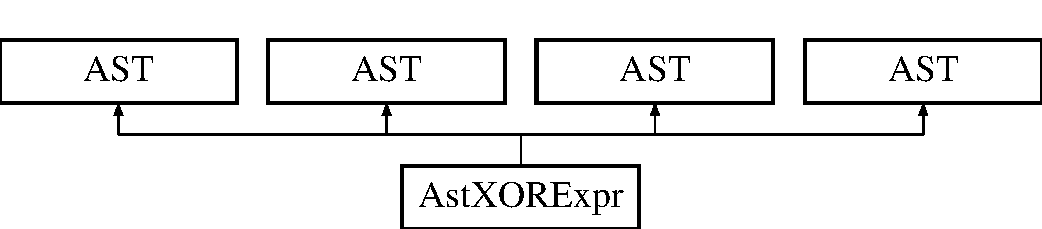
\includegraphics[height=2.000000cm]{classAstXORExpr}
\end{center}
\end{figure}
\subsection*{Public Member Functions}
\begin{DoxyCompactItemize}
\item 
\hypertarget{classAstXORExpr_a04ca42d403c3e4d69a0b9c6e22aff25b}{{\bfseries Ast\-X\-O\-R\-Expr} (\hyperlink{classAstAndExpr}{Ast\-And\-Expr} $\ast$a)}\label{classAstXORExpr_a04ca42d403c3e4d69a0b9c6e22aff25b}

\item 
\hypertarget{classAstXORExpr_a1481a0957bc4aee1819caa848f2f5a2d}{{\bfseries Ast\-X\-O\-R\-Expr} (\hyperlink{classAstXORExpr}{Ast\-X\-O\-R\-Expr} $\ast$x, \hyperlink{classAstAndExpr}{Ast\-And\-Expr} $\ast$a)}\label{classAstXORExpr_a1481a0957bc4aee1819caa848f2f5a2d}

\item 
void \hyperlink{classAstXORExpr_a6742a6024309a1359fe029204ca50c4f}{Visit} ()
\begin{DoxyCompactList}\small\item\em This function is responsible for tree traversals. \end{DoxyCompactList}\item 
void \hyperlink{classAST_a71d680856e95ff89f55d5311a552eba6}{set\-Label} (string l)
\begin{DoxyCompactList}\small\item\em Sets the label for the node. \end{DoxyCompactList}\item 
int \hyperlink{classAST_ab7a5b1d9f1c2de0d98deb356f724a42c}{get\-U\-I\-D} ()
\begin{DoxyCompactList}\small\item\em Gets the node's unique I\-D. \end{DoxyCompactList}\item 
string \hyperlink{classAST_aee029be902fffc927d16ccb03eb922ad}{get\-Label} ()
\begin{DoxyCompactList}\small\item\em Gets the node's label. \end{DoxyCompactList}\end{DoxyCompactItemize}
\subsection*{Static Public Attributes}
\begin{DoxyCompactItemize}
\item 
\hypertarget{classAST_aca9e6637209b31e03a09c0d42f29bdfa}{static \hyperlink{classVisualizer}{Visualizer} \hyperlink{classAST_aca9e6637209b31e03a09c0d42f29bdfa}{vis}}\label{classAST_aca9e6637209b31e03a09c0d42f29bdfa}

\begin{DoxyCompactList}\small\item\em Static visualizer instance for generating the visualization of the \hyperlink{classAST}{A\-S\-T}. \end{DoxyCompactList}\end{DoxyCompactItemize}
\subsection*{Protected Attributes}
\begin{DoxyCompactItemize}
\item 
\hypertarget{classAST_a847b778f1c3dd5a19de32de432ee6e15}{int \hyperlink{classAST_a847b778f1c3dd5a19de32de432ee6e15}{uid}}\label{classAST_a847b778f1c3dd5a19de32de432ee6e15}

\begin{DoxyCompactList}\small\item\em The unique id. \end{DoxyCompactList}\item 
\hypertarget{classAST_ab2e239ccc0688d2341724432ff5a1a31}{string \hyperlink{classAST_ab2e239ccc0688d2341724432ff5a1a31}{label}}\label{classAST_ab2e239ccc0688d2341724432ff5a1a31}

\begin{DoxyCompactList}\small\item\em The label to be printed in the visualization. \end{DoxyCompactList}\end{DoxyCompactItemize}
\subsection*{Private Attributes}
\begin{DoxyCompactItemize}
\item 
\hypertarget{classAstXORExpr_a7026a65e57b3ae26d8b7cf8547fc17f9}{\hyperlink{classAstAndExpr}{Ast\-And\-Expr} $\ast$ {\bfseries a}}\label{classAstXORExpr_a7026a65e57b3ae26d8b7cf8547fc17f9}

\item 
\hypertarget{classAstXORExpr_aae414bcc43b3bfc11df5aca902df486f}{\hyperlink{classAstXORExpr}{Ast\-X\-O\-R\-Expr} $\ast$ {\bfseries x}}\label{classAstXORExpr_aae414bcc43b3bfc11df5aca902df486f}

\end{DoxyCompactItemize}


\subsection{Member Function Documentation}
\hypertarget{classAST_aee029be902fffc927d16ccb03eb922ad}{\index{Ast\-X\-O\-R\-Expr@{Ast\-X\-O\-R\-Expr}!get\-Label@{get\-Label}}
\index{get\-Label@{get\-Label}!AstXORExpr@{Ast\-X\-O\-R\-Expr}}
\subsubsection[{get\-Label}]{\setlength{\rightskip}{0pt plus 5cm}string A\-S\-T\-::get\-Label (
\begin{DoxyParamCaption}
{}
\end{DoxyParamCaption}
)\hspace{0.3cm}{\ttfamily [inline]}, {\ttfamily [inherited]}}}\label{classAST_aee029be902fffc927d16ccb03eb922ad}


Gets the node's label. 

\begin{DoxyReturn}{Returns}
The label 
\end{DoxyReturn}
\hypertarget{classAST_ab7a5b1d9f1c2de0d98deb356f724a42c}{\index{Ast\-X\-O\-R\-Expr@{Ast\-X\-O\-R\-Expr}!get\-U\-I\-D@{get\-U\-I\-D}}
\index{get\-U\-I\-D@{get\-U\-I\-D}!AstXORExpr@{Ast\-X\-O\-R\-Expr}}
\subsubsection[{get\-U\-I\-D}]{\setlength{\rightskip}{0pt plus 5cm}int A\-S\-T\-::get\-U\-I\-D (
\begin{DoxyParamCaption}
{}
\end{DoxyParamCaption}
)\hspace{0.3cm}{\ttfamily [inline]}, {\ttfamily [inherited]}}}\label{classAST_ab7a5b1d9f1c2de0d98deb356f724a42c}


Gets the node's unique I\-D. 

\begin{DoxyReturn}{Returns}
The unique id 
\end{DoxyReturn}
\hypertarget{classAST_a71d680856e95ff89f55d5311a552eba6}{\index{Ast\-X\-O\-R\-Expr@{Ast\-X\-O\-R\-Expr}!set\-Label@{set\-Label}}
\index{set\-Label@{set\-Label}!AstXORExpr@{Ast\-X\-O\-R\-Expr}}
\subsubsection[{set\-Label}]{\setlength{\rightskip}{0pt plus 5cm}void A\-S\-T\-::set\-Label (
\begin{DoxyParamCaption}
\item[{string}]{l}
\end{DoxyParamCaption}
)\hspace{0.3cm}{\ttfamily [inline]}, {\ttfamily [inherited]}}}\label{classAST_a71d680856e95ff89f55d5311a552eba6}


Sets the label for the node. 


\begin{DoxyParams}{Parameters}
{\em l} & The label string \\
\hline
\end{DoxyParams}
\hypertarget{classAstXORExpr_a6742a6024309a1359fe029204ca50c4f}{\index{Ast\-X\-O\-R\-Expr@{Ast\-X\-O\-R\-Expr}!Visit@{Visit}}
\index{Visit@{Visit}!AstXORExpr@{Ast\-X\-O\-R\-Expr}}
\subsubsection[{Visit}]{\setlength{\rightskip}{0pt plus 5cm}void Ast\-X\-O\-R\-Expr\-::\-Visit (
\begin{DoxyParamCaption}
{}
\end{DoxyParamCaption}
)\hspace{0.3cm}{\ttfamily [virtual]}}}\label{classAstXORExpr_a6742a6024309a1359fe029204ca50c4f}


This function is responsible for tree traversals. 

This function will call the Visit functions of each of it's children nodes, call the visualization code for itself, and output any 3\-A\-C that can be generated at the current node. 

Reimplemented from \hyperlink{classAST_a5828cc86f2c4f1a0aeab6d7069e8fd82}{A\-S\-T}.



The documentation for this class was generated from the following files\-:\begin{DoxyCompactItemize}
\item 
Ast.\-h\item 
Ast.\-cpp\end{DoxyCompactItemize}

\hypertarget{classAVLTree}{\section{A\-V\-L\-Tree$<$ Data\-Item $>$ Class Template Reference}
\label{classAVLTree}\index{A\-V\-L\-Tree$<$ Data\-Item $>$@{A\-V\-L\-Tree$<$ Data\-Item $>$}}
}


An implementation of a balanced binary tree called an A\-V\-L tree.  




{\ttfamily \#include $<$Avl\-Tree.\-h$>$}

\subsection*{Classes}
\begin{DoxyCompactItemize}
\item 
struct \hyperlink{structAVLTree_1_1Node}{Node}
\begin{DoxyCompactList}\small\item\em A node which composes the Data\-Item template class with pointers to its children nodes in the A\-V\-L tree and the balance factor at the current node. \end{DoxyCompactList}\end{DoxyCompactItemize}
\subsection*{Public Member Functions}
\begin{DoxyCompactItemize}
\item 
\hyperlink{classAVLTree_a685459c83f9879c6c99687cd620033cc}{A\-V\-L\-Tree} ()
\begin{DoxyCompactList}\small\item\em Default A\-V\-L tree constructor. \end{DoxyCompactList}\item 
void \hyperlink{classAVLTree_a19150bcba8501c6ae6fb2b519ad64b05}{Insert} (Data\-Item item)
\begin{DoxyCompactList}\small\item\em Inserts a new node into the tree. \end{DoxyCompactList}\item 
void \hyperlink{classAVLTree_a7d45f6097e6f9f696ed80b80c8a88722}{Insert} (Data\-Item item, \hyperlink{structAVLTree_1_1Node}{Node} $\ast$\&node, int \&change)
\begin{DoxyCompactList}\small\item\em Inserts a new node into the tree. \end{DoxyCompactList}\item 
Data\-Item $\ast$ \hyperlink{classAVLTree_a8c1cdcd4e4be5f0feb9b2bad5ef08b08}{Fetch} (Data\-Item item\-To\-Find)
\begin{DoxyCompactList}\small\item\em Searches the A\-V\-L tree for a given Data\-Item. \end{DoxyCompactList}\item 
\hyperlink{structAVLTree_1_1Node}{Node} $\ast$ \hyperlink{classAVLTree_a88e4e21a384e6dc4d9be64bfd26e642e}{Find} (Data\-Item item\-To\-Find)
\begin{DoxyCompactList}\small\item\em Searches the A\-V\-L tree for a given Data\-Item. \end{DoxyCompactList}\item 
bool \hyperlink{classAVLTree_af87b660c0c905507b3210abeecff8f8f}{Contains} (Data\-Item item\-To\-Find)
\begin{DoxyCompactList}\small\item\em Checks if the given data item is in the tree or not. \end{DoxyCompactList}\item 
\hypertarget{classAVLTree_a04db67e206a1d00093ae74a6506dcf59}{void \hyperlink{classAVLTree_a04db67e206a1d00093ae74a6506dcf59}{Dump} ()}\label{classAVLTree_a04db67e206a1d00093ae74a6506dcf59}

\begin{DoxyCompactList}\small\item\em Outputs the A\-V\-L tree to stdout recursively using the insertion operator for the Data\-Item template type. \end{DoxyCompactList}\item 
\hypertarget{classAVLTree_a501149b97428fd09771c4dffc2d5d932}{list$<$ Data\-Item $>$ {\bfseries Get\-Elements} ()}\label{classAVLTree_a501149b97428fd09771c4dffc2d5d932}

\item 
\hyperlink{classAVLTree_a685459c83f9879c6c99687cd620033cc}{A\-V\-L\-Tree} ()
\begin{DoxyCompactList}\small\item\em Default A\-V\-L tree constructor. \end{DoxyCompactList}\item 
void \hyperlink{classAVLTree_a19150bcba8501c6ae6fb2b519ad64b05}{Insert} (Data\-Item item)
\begin{DoxyCompactList}\small\item\em Inserts a new node into the tree. \end{DoxyCompactList}\item 
void \hyperlink{classAVLTree_a7d45f6097e6f9f696ed80b80c8a88722}{Insert} (Data\-Item item, \hyperlink{structAVLTree_1_1Node}{Node} $\ast$\&node, int \&change)
\begin{DoxyCompactList}\small\item\em Inserts a new node into the tree. \end{DoxyCompactList}\item 
Data\-Item $\ast$ \hyperlink{classAVLTree_a8c1cdcd4e4be5f0feb9b2bad5ef08b08}{Fetch} (Data\-Item item\-To\-Find)
\begin{DoxyCompactList}\small\item\em Searches the A\-V\-L tree for a given Data\-Item. \end{DoxyCompactList}\item 
\hyperlink{structAVLTree_1_1Node}{Node} $\ast$ \hyperlink{classAVLTree_a88e4e21a384e6dc4d9be64bfd26e642e}{Find} (Data\-Item item\-To\-Find)
\begin{DoxyCompactList}\small\item\em Searches the A\-V\-L tree for a given Data\-Item. \end{DoxyCompactList}\item 
bool \hyperlink{classAVLTree_af87b660c0c905507b3210abeecff8f8f}{Contains} (Data\-Item item\-To\-Find)
\begin{DoxyCompactList}\small\item\em Checks if the given data item is in the tree or not. \end{DoxyCompactList}\item 
\hypertarget{classAVLTree_a04db67e206a1d00093ae74a6506dcf59}{void \hyperlink{classAVLTree_a04db67e206a1d00093ae74a6506dcf59}{Dump} ()}\label{classAVLTree_a04db67e206a1d00093ae74a6506dcf59}

\begin{DoxyCompactList}\small\item\em Outputs the A\-V\-L tree to stdout recursively using the insertion operator for the Data\-Item template type. \end{DoxyCompactList}\item 
\hypertarget{classAVLTree_a501149b97428fd09771c4dffc2d5d932}{list$<$ Data\-Item $>$ {\bfseries Get\-Elements} ()}\label{classAVLTree_a501149b97428fd09771c4dffc2d5d932}

\item 
\hyperlink{classAVLTree_a685459c83f9879c6c99687cd620033cc}{A\-V\-L\-Tree} ()
\begin{DoxyCompactList}\small\item\em Default A\-V\-L tree constructor. \end{DoxyCompactList}\item 
void \hyperlink{classAVLTree_a19150bcba8501c6ae6fb2b519ad64b05}{Insert} (Data\-Item item)
\begin{DoxyCompactList}\small\item\em Inserts a new node into the tree. \end{DoxyCompactList}\item 
void \hyperlink{classAVLTree_a7d45f6097e6f9f696ed80b80c8a88722}{Insert} (Data\-Item item, \hyperlink{structAVLTree_1_1Node}{Node} $\ast$\&node, int \&change)
\begin{DoxyCompactList}\small\item\em Inserts a new node into the tree. \end{DoxyCompactList}\item 
Data\-Item $\ast$ \hyperlink{classAVLTree_a8c1cdcd4e4be5f0feb9b2bad5ef08b08}{Fetch} (Data\-Item item\-To\-Find)
\begin{DoxyCompactList}\small\item\em Searches the A\-V\-L tree for a given Data\-Item. \end{DoxyCompactList}\item 
\hyperlink{structAVLTree_1_1Node}{Node} $\ast$ \hyperlink{classAVLTree_a88e4e21a384e6dc4d9be64bfd26e642e}{Find} (Data\-Item item\-To\-Find)
\begin{DoxyCompactList}\small\item\em Searches the A\-V\-L tree for a given Data\-Item. \end{DoxyCompactList}\item 
bool \hyperlink{classAVLTree_af87b660c0c905507b3210abeecff8f8f}{Contains} (Data\-Item item\-To\-Find)
\begin{DoxyCompactList}\small\item\em Checks if the given data item is in the tree or not. \end{DoxyCompactList}\item 
\hypertarget{classAVLTree_a04db67e206a1d00093ae74a6506dcf59}{void \hyperlink{classAVLTree_a04db67e206a1d00093ae74a6506dcf59}{Dump} ()}\label{classAVLTree_a04db67e206a1d00093ae74a6506dcf59}

\begin{DoxyCompactList}\small\item\em Outputs the A\-V\-L tree to stdout recursively using the insertion operator for the Data\-Item template type. \end{DoxyCompactList}\item 
\hypertarget{classAVLTree_a501149b97428fd09771c4dffc2d5d932}{list$<$ Data\-Item $>$ {\bfseries Get\-Elements} ()}\label{classAVLTree_a501149b97428fd09771c4dffc2d5d932}

\item 
\hyperlink{classAVLTree_a685459c83f9879c6c99687cd620033cc}{A\-V\-L\-Tree} ()
\begin{DoxyCompactList}\small\item\em Default A\-V\-L tree constructor. \end{DoxyCompactList}\item 
void \hyperlink{classAVLTree_a19150bcba8501c6ae6fb2b519ad64b05}{Insert} (Data\-Item item)
\begin{DoxyCompactList}\small\item\em Inserts a new node into the tree. \end{DoxyCompactList}\item 
void \hyperlink{classAVLTree_a7d45f6097e6f9f696ed80b80c8a88722}{Insert} (Data\-Item item, \hyperlink{structAVLTree_1_1Node}{Node} $\ast$\&node, int \&change)
\begin{DoxyCompactList}\small\item\em Inserts a new node into the tree. \end{DoxyCompactList}\item 
Data\-Item $\ast$ \hyperlink{classAVLTree_a8c1cdcd4e4be5f0feb9b2bad5ef08b08}{Fetch} (Data\-Item item\-To\-Find)
\begin{DoxyCompactList}\small\item\em Searches the A\-V\-L tree for a given Data\-Item. \end{DoxyCompactList}\item 
\hyperlink{structAVLTree_1_1Node}{Node} $\ast$ \hyperlink{classAVLTree_a88e4e21a384e6dc4d9be64bfd26e642e}{Find} (Data\-Item item\-To\-Find)
\begin{DoxyCompactList}\small\item\em Searches the A\-V\-L tree for a given Data\-Item. \end{DoxyCompactList}\item 
bool \hyperlink{classAVLTree_af87b660c0c905507b3210abeecff8f8f}{Contains} (Data\-Item item\-To\-Find)
\begin{DoxyCompactList}\small\item\em Checks if the given data item is in the tree or not. \end{DoxyCompactList}\item 
\hypertarget{classAVLTree_a04db67e206a1d00093ae74a6506dcf59}{void \hyperlink{classAVLTree_a04db67e206a1d00093ae74a6506dcf59}{Dump} ()}\label{classAVLTree_a04db67e206a1d00093ae74a6506dcf59}

\begin{DoxyCompactList}\small\item\em Outputs the A\-V\-L tree to stdout recursively using the insertion operator for the Data\-Item template type. \end{DoxyCompactList}\item 
\hypertarget{classAVLTree_a501149b97428fd09771c4dffc2d5d932}{list$<$ Data\-Item $>$ {\bfseries Get\-Elements} ()}\label{classAVLTree_a501149b97428fd09771c4dffc2d5d932}

\item 
\hyperlink{classAVLTree_a685459c83f9879c6c99687cd620033cc}{A\-V\-L\-Tree} ()
\begin{DoxyCompactList}\small\item\em Default A\-V\-L tree constructor. \end{DoxyCompactList}\item 
void \hyperlink{classAVLTree_a19150bcba8501c6ae6fb2b519ad64b05}{Insert} (Data\-Item item)
\begin{DoxyCompactList}\small\item\em Inserts a new node into the tree. \end{DoxyCompactList}\item 
void \hyperlink{classAVLTree_a7d45f6097e6f9f696ed80b80c8a88722}{Insert} (Data\-Item item, \hyperlink{structAVLTree_1_1Node}{Node} $\ast$\&node, int \&change)
\begin{DoxyCompactList}\small\item\em Inserts a new node into the tree. \end{DoxyCompactList}\item 
Data\-Item $\ast$ \hyperlink{classAVLTree_a8c1cdcd4e4be5f0feb9b2bad5ef08b08}{Fetch} (Data\-Item item\-To\-Find)
\begin{DoxyCompactList}\small\item\em Searches the A\-V\-L tree for a given Data\-Item. \end{DoxyCompactList}\item 
\hyperlink{structAVLTree_1_1Node}{Node} $\ast$ \hyperlink{classAVLTree_a88e4e21a384e6dc4d9be64bfd26e642e}{Find} (Data\-Item item\-To\-Find)
\begin{DoxyCompactList}\small\item\em Searches the A\-V\-L tree for a given Data\-Item. \end{DoxyCompactList}\item 
bool \hyperlink{classAVLTree_af87b660c0c905507b3210abeecff8f8f}{Contains} (Data\-Item item\-To\-Find)
\begin{DoxyCompactList}\small\item\em Checks if the given data item is in the tree or not. \end{DoxyCompactList}\item 
\hypertarget{classAVLTree_a04db67e206a1d00093ae74a6506dcf59}{void \hyperlink{classAVLTree_a04db67e206a1d00093ae74a6506dcf59}{Dump} ()}\label{classAVLTree_a04db67e206a1d00093ae74a6506dcf59}

\begin{DoxyCompactList}\small\item\em Outputs the A\-V\-L tree to stdout recursively using the insertion operator for the Data\-Item template type. \end{DoxyCompactList}\item 
\hypertarget{classAVLTree_a501149b97428fd09771c4dffc2d5d932}{list$<$ Data\-Item $>$ {\bfseries Get\-Elements} ()}\label{classAVLTree_a501149b97428fd09771c4dffc2d5d932}

\item 
\hyperlink{classAVLTree_a685459c83f9879c6c99687cd620033cc}{A\-V\-L\-Tree} ()
\begin{DoxyCompactList}\small\item\em Default A\-V\-L tree constructor. \end{DoxyCompactList}\item 
void \hyperlink{classAVLTree_a19150bcba8501c6ae6fb2b519ad64b05}{Insert} (Data\-Item item)
\begin{DoxyCompactList}\small\item\em Inserts a new node into the tree. \end{DoxyCompactList}\item 
void \hyperlink{classAVLTree_a7d45f6097e6f9f696ed80b80c8a88722}{Insert} (Data\-Item item, \hyperlink{structAVLTree_1_1Node}{Node} $\ast$\&node, int \&change)
\begin{DoxyCompactList}\small\item\em Inserts a new node into the tree. \end{DoxyCompactList}\item 
Data\-Item $\ast$ \hyperlink{classAVLTree_a8c1cdcd4e4be5f0feb9b2bad5ef08b08}{Fetch} (Data\-Item item\-To\-Find)
\begin{DoxyCompactList}\small\item\em Searches the A\-V\-L tree for a given Data\-Item. \end{DoxyCompactList}\item 
\hyperlink{structAVLTree_1_1Node}{Node} $\ast$ \hyperlink{classAVLTree_a88e4e21a384e6dc4d9be64bfd26e642e}{Find} (Data\-Item item\-To\-Find)
\begin{DoxyCompactList}\small\item\em Searches the A\-V\-L tree for a given Data\-Item. \end{DoxyCompactList}\item 
bool \hyperlink{classAVLTree_af87b660c0c905507b3210abeecff8f8f}{Contains} (Data\-Item item\-To\-Find)
\begin{DoxyCompactList}\small\item\em Checks if the given data item is in the tree or not. \end{DoxyCompactList}\item 
\hypertarget{classAVLTree_a04db67e206a1d00093ae74a6506dcf59}{void \hyperlink{classAVLTree_a04db67e206a1d00093ae74a6506dcf59}{Dump} ()}\label{classAVLTree_a04db67e206a1d00093ae74a6506dcf59}

\begin{DoxyCompactList}\small\item\em Outputs the A\-V\-L tree to stdout recursively using the insertion operator for the Data\-Item template type. \end{DoxyCompactList}\item 
\hypertarget{classAVLTree_a501149b97428fd09771c4dffc2d5d932}{list$<$ Data\-Item $>$ {\bfseries Get\-Elements} ()}\label{classAVLTree_a501149b97428fd09771c4dffc2d5d932}

\item 
\hyperlink{classAVLTree_a685459c83f9879c6c99687cd620033cc}{A\-V\-L\-Tree} ()
\begin{DoxyCompactList}\small\item\em Default A\-V\-L tree constructor. \end{DoxyCompactList}\item 
void \hyperlink{classAVLTree_a19150bcba8501c6ae6fb2b519ad64b05}{Insert} (Data\-Item item)
\begin{DoxyCompactList}\small\item\em Inserts a new node into the tree. \end{DoxyCompactList}\item 
void \hyperlink{classAVLTree_a7d45f6097e6f9f696ed80b80c8a88722}{Insert} (Data\-Item item, \hyperlink{structAVLTree_1_1Node}{Node} $\ast$\&node, int \&change)
\begin{DoxyCompactList}\small\item\em Inserts a new node into the tree. \end{DoxyCompactList}\item 
Data\-Item $\ast$ \hyperlink{classAVLTree_a8c1cdcd4e4be5f0feb9b2bad5ef08b08}{Fetch} (Data\-Item item\-To\-Find)
\begin{DoxyCompactList}\small\item\em Searches the A\-V\-L tree for a given Data\-Item. \end{DoxyCompactList}\item 
\hyperlink{structAVLTree_1_1Node}{Node} $\ast$ \hyperlink{classAVLTree_a88e4e21a384e6dc4d9be64bfd26e642e}{Find} (Data\-Item item\-To\-Find)
\begin{DoxyCompactList}\small\item\em Searches the A\-V\-L tree for a given Data\-Item. \end{DoxyCompactList}\item 
bool \hyperlink{classAVLTree_af87b660c0c905507b3210abeecff8f8f}{Contains} (Data\-Item item\-To\-Find)
\begin{DoxyCompactList}\small\item\em Checks if the given data item is in the tree or not. \end{DoxyCompactList}\item 
\hypertarget{classAVLTree_a04db67e206a1d00093ae74a6506dcf59}{void \hyperlink{classAVLTree_a04db67e206a1d00093ae74a6506dcf59}{Dump} ()}\label{classAVLTree_a04db67e206a1d00093ae74a6506dcf59}

\begin{DoxyCompactList}\small\item\em Outputs the A\-V\-L tree to stdout recursively using the insertion operator for the Data\-Item template type. \end{DoxyCompactList}\item 
\hypertarget{classAVLTree_a501149b97428fd09771c4dffc2d5d932}{list$<$ Data\-Item $>$ {\bfseries Get\-Elements} ()}\label{classAVLTree_a501149b97428fd09771c4dffc2d5d932}

\item 
\hyperlink{classAVLTree_a685459c83f9879c6c99687cd620033cc}{A\-V\-L\-Tree} ()
\begin{DoxyCompactList}\small\item\em Default A\-V\-L tree constructor. \end{DoxyCompactList}\item 
void \hyperlink{classAVLTree_a19150bcba8501c6ae6fb2b519ad64b05}{Insert} (Data\-Item item)
\begin{DoxyCompactList}\small\item\em Inserts a new node into the tree. \end{DoxyCompactList}\item 
void \hyperlink{classAVLTree_a7d45f6097e6f9f696ed80b80c8a88722}{Insert} (Data\-Item item, \hyperlink{structAVLTree_1_1Node}{Node} $\ast$\&node, int \&change)
\begin{DoxyCompactList}\small\item\em Inserts a new node into the tree. \end{DoxyCompactList}\item 
Data\-Item $\ast$ \hyperlink{classAVLTree_a8c1cdcd4e4be5f0feb9b2bad5ef08b08}{Fetch} (Data\-Item item\-To\-Find)
\begin{DoxyCompactList}\small\item\em Searches the A\-V\-L tree for a given Data\-Item. \end{DoxyCompactList}\item 
\hyperlink{structAVLTree_1_1Node}{Node} $\ast$ \hyperlink{classAVLTree_a88e4e21a384e6dc4d9be64bfd26e642e}{Find} (Data\-Item item\-To\-Find)
\begin{DoxyCompactList}\small\item\em Searches the A\-V\-L tree for a given Data\-Item. \end{DoxyCompactList}\item 
bool \hyperlink{classAVLTree_af87b660c0c905507b3210abeecff8f8f}{Contains} (Data\-Item item\-To\-Find)
\begin{DoxyCompactList}\small\item\em Checks if the given data item is in the tree or not. \end{DoxyCompactList}\item 
\hypertarget{classAVLTree_a04db67e206a1d00093ae74a6506dcf59}{void \hyperlink{classAVLTree_a04db67e206a1d00093ae74a6506dcf59}{Dump} ()}\label{classAVLTree_a04db67e206a1d00093ae74a6506dcf59}

\begin{DoxyCompactList}\small\item\em Outputs the A\-V\-L tree to stdout recursively using the insertion operator for the Data\-Item template type. \end{DoxyCompactList}\item 
\hypertarget{classAVLTree_a501149b97428fd09771c4dffc2d5d932}{list$<$ Data\-Item $>$ {\bfseries Get\-Elements} ()}\label{classAVLTree_a501149b97428fd09771c4dffc2d5d932}

\item 
\hyperlink{classAVLTree_a685459c83f9879c6c99687cd620033cc}{A\-V\-L\-Tree} ()
\begin{DoxyCompactList}\small\item\em Default A\-V\-L tree constructor. \end{DoxyCompactList}\item 
void \hyperlink{classAVLTree_a19150bcba8501c6ae6fb2b519ad64b05}{Insert} (Data\-Item item)
\begin{DoxyCompactList}\small\item\em Inserts a new node into the tree. \end{DoxyCompactList}\item 
void \hyperlink{classAVLTree_a7d45f6097e6f9f696ed80b80c8a88722}{Insert} (Data\-Item item, \hyperlink{structAVLTree_1_1Node}{Node} $\ast$\&node, int \&change)
\begin{DoxyCompactList}\small\item\em Inserts a new node into the tree. \end{DoxyCompactList}\item 
Data\-Item $\ast$ \hyperlink{classAVLTree_a8c1cdcd4e4be5f0feb9b2bad5ef08b08}{Fetch} (Data\-Item item\-To\-Find)
\begin{DoxyCompactList}\small\item\em Searches the A\-V\-L tree for a given Data\-Item. \end{DoxyCompactList}\item 
\hyperlink{structAVLTree_1_1Node}{Node} $\ast$ \hyperlink{classAVLTree_a88e4e21a384e6dc4d9be64bfd26e642e}{Find} (Data\-Item item\-To\-Find)
\begin{DoxyCompactList}\small\item\em Searches the A\-V\-L tree for a given Data\-Item. \end{DoxyCompactList}\item 
bool \hyperlink{classAVLTree_af87b660c0c905507b3210abeecff8f8f}{Contains} (Data\-Item item\-To\-Find)
\begin{DoxyCompactList}\small\item\em Checks if the given data item is in the tree or not. \end{DoxyCompactList}\item 
\hypertarget{classAVLTree_a04db67e206a1d00093ae74a6506dcf59}{void \hyperlink{classAVLTree_a04db67e206a1d00093ae74a6506dcf59}{Dump} ()}\label{classAVLTree_a04db67e206a1d00093ae74a6506dcf59}

\begin{DoxyCompactList}\small\item\em Outputs the A\-V\-L tree to stdout recursively using the insertion operator for the Data\-Item template type. \end{DoxyCompactList}\item 
\hypertarget{classAVLTree_a501149b97428fd09771c4dffc2d5d932}{list$<$ Data\-Item $>$ {\bfseries Get\-Elements} ()}\label{classAVLTree_a501149b97428fd09771c4dffc2d5d932}

\item 
\hyperlink{classAVLTree_a685459c83f9879c6c99687cd620033cc}{A\-V\-L\-Tree} ()
\begin{DoxyCompactList}\small\item\em Default A\-V\-L tree constructor. \end{DoxyCompactList}\item 
void \hyperlink{classAVLTree_a19150bcba8501c6ae6fb2b519ad64b05}{Insert} (Data\-Item item)
\begin{DoxyCompactList}\small\item\em Inserts a new node into the tree. \end{DoxyCompactList}\item 
void \hyperlink{classAVLTree_a7d45f6097e6f9f696ed80b80c8a88722}{Insert} (Data\-Item item, \hyperlink{structAVLTree_1_1Node}{Node} $\ast$\&node, int \&change)
\begin{DoxyCompactList}\small\item\em Inserts a new node into the tree. \end{DoxyCompactList}\item 
Data\-Item $\ast$ \hyperlink{classAVLTree_a8c1cdcd4e4be5f0feb9b2bad5ef08b08}{Fetch} (Data\-Item item\-To\-Find)
\begin{DoxyCompactList}\small\item\em Searches the A\-V\-L tree for a given Data\-Item. \end{DoxyCompactList}\item 
\hyperlink{structAVLTree_1_1Node}{Node} $\ast$ \hyperlink{classAVLTree_a88e4e21a384e6dc4d9be64bfd26e642e}{Find} (Data\-Item item\-To\-Find)
\begin{DoxyCompactList}\small\item\em Searches the A\-V\-L tree for a given Data\-Item. \end{DoxyCompactList}\item 
bool \hyperlink{classAVLTree_af87b660c0c905507b3210abeecff8f8f}{Contains} (Data\-Item item\-To\-Find)
\begin{DoxyCompactList}\small\item\em Checks if the given data item is in the tree or not. \end{DoxyCompactList}\item 
\hypertarget{classAVLTree_a04db67e206a1d00093ae74a6506dcf59}{void \hyperlink{classAVLTree_a04db67e206a1d00093ae74a6506dcf59}{Dump} ()}\label{classAVLTree_a04db67e206a1d00093ae74a6506dcf59}

\begin{DoxyCompactList}\small\item\em Outputs the A\-V\-L tree to stdout recursively using the insertion operator for the Data\-Item template type. \end{DoxyCompactList}\item 
\hypertarget{classAVLTree_a501149b97428fd09771c4dffc2d5d932}{list$<$ Data\-Item $>$ {\bfseries Get\-Elements} ()}\label{classAVLTree_a501149b97428fd09771c4dffc2d5d932}

\end{DoxyCompactItemize}
\subsection*{Private Member Functions}
\begin{DoxyCompactItemize}
\item 
int \hyperlink{classAVLTree_ac7ebd1be164c8e1d0eab990e14285957}{Single\-Rotate} (\hyperlink{structAVLTree_1_1Node}{Node} $\ast$\&root\-Node, int direction)
\begin{DoxyCompactList}\small\item\em Performs a single rotation in the indicated direction and about the specified node. \end{DoxyCompactList}\item 
int \hyperlink{classAVLTree_a7e2ed1a8d70f97fc9d4de6d9da4eb729}{Double\-Rotate} (\hyperlink{structAVLTree_1_1Node}{Node} $\ast$\&root\-Node, int direction)
\begin{DoxyCompactList}\small\item\em Performs a double rotation in the indicated direction and about the specified node. \end{DoxyCompactList}\item 
int \hyperlink{classAVLTree_aabcb2e90d12bcb172f728692bce7e7be}{Balance} (\hyperlink{structAVLTree_1_1Node}{Node} $\ast$\&root\-Node)
\begin{DoxyCompactList}\small\item\em Balances the tree beginning at the provided root node using single and double rotations. \end{DoxyCompactList}\item 
void \hyperlink{classAVLTree_aeafa2839058227c9a076d56d7929ebf7}{Dump} (\hyperlink{structAVLTree_1_1Node}{Node} $\ast$node)
\begin{DoxyCompactList}\small\item\em Outputs the A\-V\-L tree to stdout using the $<$$<$ operator of the provided Data\-Item template type. \end{DoxyCompactList}\item 
\hypertarget{classAVLTree_ad02b6a7bd1582dba503d48a8b960d902}{list$<$ Data\-Item $>$ {\bfseries Get\-Elements} (\hyperlink{structAVLTree_1_1Node}{Node} $\ast$node)}\label{classAVLTree_ad02b6a7bd1582dba503d48a8b960d902}

\item 
int \hyperlink{classAVLTree_ac7ebd1be164c8e1d0eab990e14285957}{Single\-Rotate} (\hyperlink{structAVLTree_1_1Node}{Node} $\ast$\&root\-Node, int direction)
\begin{DoxyCompactList}\small\item\em Performs a single rotation in the indicated direction and about the specified node. \end{DoxyCompactList}\item 
int \hyperlink{classAVLTree_a7e2ed1a8d70f97fc9d4de6d9da4eb729}{Double\-Rotate} (\hyperlink{structAVLTree_1_1Node}{Node} $\ast$\&root\-Node, int direction)
\begin{DoxyCompactList}\small\item\em Performs a double rotation in the indicated direction and about the specified node. \end{DoxyCompactList}\item 
int \hyperlink{classAVLTree_aabcb2e90d12bcb172f728692bce7e7be}{Balance} (\hyperlink{structAVLTree_1_1Node}{Node} $\ast$\&root\-Node)
\begin{DoxyCompactList}\small\item\em Balances the tree beginning at the provided root node using single and double rotations. \end{DoxyCompactList}\item 
void \hyperlink{classAVLTree_aeafa2839058227c9a076d56d7929ebf7}{Dump} (\hyperlink{structAVLTree_1_1Node}{Node} $\ast$node)
\begin{DoxyCompactList}\small\item\em Outputs the A\-V\-L tree to stdout using the $<$$<$ operator of the provided Data\-Item template type. \end{DoxyCompactList}\item 
\hypertarget{classAVLTree_ad02b6a7bd1582dba503d48a8b960d902}{list$<$ Data\-Item $>$ {\bfseries Get\-Elements} (\hyperlink{structAVLTree_1_1Node}{Node} $\ast$node)}\label{classAVLTree_ad02b6a7bd1582dba503d48a8b960d902}

\item 
int \hyperlink{classAVLTree_ac7ebd1be164c8e1d0eab990e14285957}{Single\-Rotate} (\hyperlink{structAVLTree_1_1Node}{Node} $\ast$\&root\-Node, int direction)
\begin{DoxyCompactList}\small\item\em Performs a single rotation in the indicated direction and about the specified node. \end{DoxyCompactList}\item 
int \hyperlink{classAVLTree_a7e2ed1a8d70f97fc9d4de6d9da4eb729}{Double\-Rotate} (\hyperlink{structAVLTree_1_1Node}{Node} $\ast$\&root\-Node, int direction)
\begin{DoxyCompactList}\small\item\em Performs a double rotation in the indicated direction and about the specified node. \end{DoxyCompactList}\item 
int \hyperlink{classAVLTree_aabcb2e90d12bcb172f728692bce7e7be}{Balance} (\hyperlink{structAVLTree_1_1Node}{Node} $\ast$\&root\-Node)
\begin{DoxyCompactList}\small\item\em Balances the tree beginning at the provided root node using single and double rotations. \end{DoxyCompactList}\item 
void \hyperlink{classAVLTree_aeafa2839058227c9a076d56d7929ebf7}{Dump} (\hyperlink{structAVLTree_1_1Node}{Node} $\ast$node)
\begin{DoxyCompactList}\small\item\em Outputs the A\-V\-L tree to stdout using the $<$$<$ operator of the provided Data\-Item template type. \end{DoxyCompactList}\item 
\hypertarget{classAVLTree_ad02b6a7bd1582dba503d48a8b960d902}{list$<$ Data\-Item $>$ {\bfseries Get\-Elements} (\hyperlink{structAVLTree_1_1Node}{Node} $\ast$node)}\label{classAVLTree_ad02b6a7bd1582dba503d48a8b960d902}

\item 
int \hyperlink{classAVLTree_ac7ebd1be164c8e1d0eab990e14285957}{Single\-Rotate} (\hyperlink{structAVLTree_1_1Node}{Node} $\ast$\&root\-Node, int direction)
\begin{DoxyCompactList}\small\item\em Performs a single rotation in the indicated direction and about the specified node. \end{DoxyCompactList}\item 
int \hyperlink{classAVLTree_a7e2ed1a8d70f97fc9d4de6d9da4eb729}{Double\-Rotate} (\hyperlink{structAVLTree_1_1Node}{Node} $\ast$\&root\-Node, int direction)
\begin{DoxyCompactList}\small\item\em Performs a double rotation in the indicated direction and about the specified node. \end{DoxyCompactList}\item 
int \hyperlink{classAVLTree_aabcb2e90d12bcb172f728692bce7e7be}{Balance} (\hyperlink{structAVLTree_1_1Node}{Node} $\ast$\&root\-Node)
\begin{DoxyCompactList}\small\item\em Balances the tree beginning at the provided root node using single and double rotations. \end{DoxyCompactList}\item 
void \hyperlink{classAVLTree_aeafa2839058227c9a076d56d7929ebf7}{Dump} (\hyperlink{structAVLTree_1_1Node}{Node} $\ast$node)
\begin{DoxyCompactList}\small\item\em Outputs the A\-V\-L tree to stdout using the $<$$<$ operator of the provided Data\-Item template type. \end{DoxyCompactList}\item 
\hypertarget{classAVLTree_ad02b6a7bd1582dba503d48a8b960d902}{list$<$ Data\-Item $>$ {\bfseries Get\-Elements} (\hyperlink{structAVLTree_1_1Node}{Node} $\ast$node)}\label{classAVLTree_ad02b6a7bd1582dba503d48a8b960d902}

\item 
int \hyperlink{classAVLTree_ac7ebd1be164c8e1d0eab990e14285957}{Single\-Rotate} (\hyperlink{structAVLTree_1_1Node}{Node} $\ast$\&root\-Node, int direction)
\begin{DoxyCompactList}\small\item\em Performs a single rotation in the indicated direction and about the specified node. \end{DoxyCompactList}\item 
int \hyperlink{classAVLTree_a7e2ed1a8d70f97fc9d4de6d9da4eb729}{Double\-Rotate} (\hyperlink{structAVLTree_1_1Node}{Node} $\ast$\&root\-Node, int direction)
\begin{DoxyCompactList}\small\item\em Performs a double rotation in the indicated direction and about the specified node. \end{DoxyCompactList}\item 
int \hyperlink{classAVLTree_aabcb2e90d12bcb172f728692bce7e7be}{Balance} (\hyperlink{structAVLTree_1_1Node}{Node} $\ast$\&root\-Node)
\begin{DoxyCompactList}\small\item\em Balances the tree beginning at the provided root node using single and double rotations. \end{DoxyCompactList}\item 
void \hyperlink{classAVLTree_aeafa2839058227c9a076d56d7929ebf7}{Dump} (\hyperlink{structAVLTree_1_1Node}{Node} $\ast$node)
\begin{DoxyCompactList}\small\item\em Outputs the A\-V\-L tree to stdout using the $<$$<$ operator of the provided Data\-Item template type. \end{DoxyCompactList}\item 
\hypertarget{classAVLTree_ad02b6a7bd1582dba503d48a8b960d902}{list$<$ Data\-Item $>$ {\bfseries Get\-Elements} (\hyperlink{structAVLTree_1_1Node}{Node} $\ast$node)}\label{classAVLTree_ad02b6a7bd1582dba503d48a8b960d902}

\item 
int \hyperlink{classAVLTree_ac7ebd1be164c8e1d0eab990e14285957}{Single\-Rotate} (\hyperlink{structAVLTree_1_1Node}{Node} $\ast$\&root\-Node, int direction)
\begin{DoxyCompactList}\small\item\em Performs a single rotation in the indicated direction and about the specified node. \end{DoxyCompactList}\item 
int \hyperlink{classAVLTree_a7e2ed1a8d70f97fc9d4de6d9da4eb729}{Double\-Rotate} (\hyperlink{structAVLTree_1_1Node}{Node} $\ast$\&root\-Node, int direction)
\begin{DoxyCompactList}\small\item\em Performs a double rotation in the indicated direction and about the specified node. \end{DoxyCompactList}\item 
int \hyperlink{classAVLTree_aabcb2e90d12bcb172f728692bce7e7be}{Balance} (\hyperlink{structAVLTree_1_1Node}{Node} $\ast$\&root\-Node)
\begin{DoxyCompactList}\small\item\em Balances the tree beginning at the provided root node using single and double rotations. \end{DoxyCompactList}\item 
void \hyperlink{classAVLTree_aeafa2839058227c9a076d56d7929ebf7}{Dump} (\hyperlink{structAVLTree_1_1Node}{Node} $\ast$node)
\begin{DoxyCompactList}\small\item\em Outputs the A\-V\-L tree to stdout using the $<$$<$ operator of the provided Data\-Item template type. \end{DoxyCompactList}\item 
\hypertarget{classAVLTree_ad02b6a7bd1582dba503d48a8b960d902}{list$<$ Data\-Item $>$ {\bfseries Get\-Elements} (\hyperlink{structAVLTree_1_1Node}{Node} $\ast$node)}\label{classAVLTree_ad02b6a7bd1582dba503d48a8b960d902}

\item 
int \hyperlink{classAVLTree_ac7ebd1be164c8e1d0eab990e14285957}{Single\-Rotate} (\hyperlink{structAVLTree_1_1Node}{Node} $\ast$\&root\-Node, int direction)
\begin{DoxyCompactList}\small\item\em Performs a single rotation in the indicated direction and about the specified node. \end{DoxyCompactList}\item 
int \hyperlink{classAVLTree_a7e2ed1a8d70f97fc9d4de6d9da4eb729}{Double\-Rotate} (\hyperlink{structAVLTree_1_1Node}{Node} $\ast$\&root\-Node, int direction)
\begin{DoxyCompactList}\small\item\em Performs a double rotation in the indicated direction and about the specified node. \end{DoxyCompactList}\item 
int \hyperlink{classAVLTree_aabcb2e90d12bcb172f728692bce7e7be}{Balance} (\hyperlink{structAVLTree_1_1Node}{Node} $\ast$\&root\-Node)
\begin{DoxyCompactList}\small\item\em Balances the tree beginning at the provided root node using single and double rotations. \end{DoxyCompactList}\item 
void \hyperlink{classAVLTree_aeafa2839058227c9a076d56d7929ebf7}{Dump} (\hyperlink{structAVLTree_1_1Node}{Node} $\ast$node)
\begin{DoxyCompactList}\small\item\em Outputs the A\-V\-L tree to stdout using the $<$$<$ operator of the provided Data\-Item template type. \end{DoxyCompactList}\item 
\hypertarget{classAVLTree_ad02b6a7bd1582dba503d48a8b960d902}{list$<$ Data\-Item $>$ {\bfseries Get\-Elements} (\hyperlink{structAVLTree_1_1Node}{Node} $\ast$node)}\label{classAVLTree_ad02b6a7bd1582dba503d48a8b960d902}

\item 
int \hyperlink{classAVLTree_ac7ebd1be164c8e1d0eab990e14285957}{Single\-Rotate} (\hyperlink{structAVLTree_1_1Node}{Node} $\ast$\&root\-Node, int direction)
\begin{DoxyCompactList}\small\item\em Performs a single rotation in the indicated direction and about the specified node. \end{DoxyCompactList}\item 
int \hyperlink{classAVLTree_a7e2ed1a8d70f97fc9d4de6d9da4eb729}{Double\-Rotate} (\hyperlink{structAVLTree_1_1Node}{Node} $\ast$\&root\-Node, int direction)
\begin{DoxyCompactList}\small\item\em Performs a double rotation in the indicated direction and about the specified node. \end{DoxyCompactList}\item 
int \hyperlink{classAVLTree_aabcb2e90d12bcb172f728692bce7e7be}{Balance} (\hyperlink{structAVLTree_1_1Node}{Node} $\ast$\&root\-Node)
\begin{DoxyCompactList}\small\item\em Balances the tree beginning at the provided root node using single and double rotations. \end{DoxyCompactList}\item 
void \hyperlink{classAVLTree_aeafa2839058227c9a076d56d7929ebf7}{Dump} (\hyperlink{structAVLTree_1_1Node}{Node} $\ast$node)
\begin{DoxyCompactList}\small\item\em Outputs the A\-V\-L tree to stdout using the $<$$<$ operator of the provided Data\-Item template type. \end{DoxyCompactList}\item 
\hypertarget{classAVLTree_ad02b6a7bd1582dba503d48a8b960d902}{list$<$ Data\-Item $>$ {\bfseries Get\-Elements} (\hyperlink{structAVLTree_1_1Node}{Node} $\ast$node)}\label{classAVLTree_ad02b6a7bd1582dba503d48a8b960d902}

\item 
int \hyperlink{classAVLTree_ac7ebd1be164c8e1d0eab990e14285957}{Single\-Rotate} (\hyperlink{structAVLTree_1_1Node}{Node} $\ast$\&root\-Node, int direction)
\begin{DoxyCompactList}\small\item\em Performs a single rotation in the indicated direction and about the specified node. \end{DoxyCompactList}\item 
int \hyperlink{classAVLTree_a7e2ed1a8d70f97fc9d4de6d9da4eb729}{Double\-Rotate} (\hyperlink{structAVLTree_1_1Node}{Node} $\ast$\&root\-Node, int direction)
\begin{DoxyCompactList}\small\item\em Performs a double rotation in the indicated direction and about the specified node. \end{DoxyCompactList}\item 
int \hyperlink{classAVLTree_aabcb2e90d12bcb172f728692bce7e7be}{Balance} (\hyperlink{structAVLTree_1_1Node}{Node} $\ast$\&root\-Node)
\begin{DoxyCompactList}\small\item\em Balances the tree beginning at the provided root node using single and double rotations. \end{DoxyCompactList}\item 
void \hyperlink{classAVLTree_aeafa2839058227c9a076d56d7929ebf7}{Dump} (\hyperlink{structAVLTree_1_1Node}{Node} $\ast$node)
\begin{DoxyCompactList}\small\item\em Outputs the A\-V\-L tree to stdout using the $<$$<$ operator of the provided Data\-Item template type. \end{DoxyCompactList}\item 
\hypertarget{classAVLTree_ad02b6a7bd1582dba503d48a8b960d902}{list$<$ Data\-Item $>$ {\bfseries Get\-Elements} (\hyperlink{structAVLTree_1_1Node}{Node} $\ast$node)}\label{classAVLTree_ad02b6a7bd1582dba503d48a8b960d902}

\item 
int \hyperlink{classAVLTree_ac7ebd1be164c8e1d0eab990e14285957}{Single\-Rotate} (\hyperlink{structAVLTree_1_1Node}{Node} $\ast$\&root\-Node, int direction)
\begin{DoxyCompactList}\small\item\em Performs a single rotation in the indicated direction and about the specified node. \end{DoxyCompactList}\item 
int \hyperlink{classAVLTree_a7e2ed1a8d70f97fc9d4de6d9da4eb729}{Double\-Rotate} (\hyperlink{structAVLTree_1_1Node}{Node} $\ast$\&root\-Node, int direction)
\begin{DoxyCompactList}\small\item\em Performs a double rotation in the indicated direction and about the specified node. \end{DoxyCompactList}\item 
int \hyperlink{classAVLTree_aabcb2e90d12bcb172f728692bce7e7be}{Balance} (\hyperlink{structAVLTree_1_1Node}{Node} $\ast$\&root\-Node)
\begin{DoxyCompactList}\small\item\em Balances the tree beginning at the provided root node using single and double rotations. \end{DoxyCompactList}\item 
void \hyperlink{classAVLTree_aeafa2839058227c9a076d56d7929ebf7}{Dump} (\hyperlink{structAVLTree_1_1Node}{Node} $\ast$node)
\begin{DoxyCompactList}\small\item\em Outputs the A\-V\-L tree to stdout using the $<$$<$ operator of the provided Data\-Item template type. \end{DoxyCompactList}\item 
\hypertarget{classAVLTree_ad02b6a7bd1582dba503d48a8b960d902}{list$<$ Data\-Item $>$ {\bfseries Get\-Elements} (\hyperlink{structAVLTree_1_1Node}{Node} $\ast$node)}\label{classAVLTree_ad02b6a7bd1582dba503d48a8b960d902}

\end{DoxyCompactItemize}
\subsection*{Private Attributes}
\begin{DoxyCompactItemize}
\item 
\hypertarget{classAVLTree_a2a00e66c783f63a166ae0f8a5b7fbe7e}{\hyperlink{structAVLTree_1_1Node}{Node} $\ast$ \hyperlink{classAVLTree_a2a00e66c783f63a166ae0f8a5b7fbe7e}{root}}\label{classAVLTree_a2a00e66c783f63a166ae0f8a5b7fbe7e}

\begin{DoxyCompactList}\small\item\em Root node of the A\-V\-L tree. \end{DoxyCompactList}\item 
\hypertarget{classAVLTree_a45c7b885186ba43a5949ed864f0c54dd}{list$<$ Data\-Item $>$ {\bfseries elements}}\label{classAVLTree_a45c7b885186ba43a5949ed864f0c54dd}

\end{DoxyCompactItemize}


\subsection{Detailed Description}
\subsubsection*{template$<$class Data\-Item$>$class A\-V\-L\-Tree$<$ Data\-Item $>$}

An implementation of a balanced binary tree called an A\-V\-L tree. 

This implementation assumes that the Data\-Item template class implements the operators $<$ (less than), $>$ (greater than), == (equality), and $<$$<$ (insertion). 

Definition at line 34 of file Avl\-Tree.\-h.



\subsection{Constructor \& Destructor Documentation}
\hypertarget{classAVLTree_a685459c83f9879c6c99687cd620033cc}{\index{A\-V\-L\-Tree@{A\-V\-L\-Tree}!A\-V\-L\-Tree@{A\-V\-L\-Tree}}
\index{A\-V\-L\-Tree@{A\-V\-L\-Tree}!AVLTree@{A\-V\-L\-Tree}}
\subsubsection[{A\-V\-L\-Tree}]{\setlength{\rightskip}{0pt plus 5cm}template$<$class Data\-Item$>$ {\bf A\-V\-L\-Tree}$<$ Data\-Item $>$\-::{\bf A\-V\-L\-Tree} (
\begin{DoxyParamCaption}
{}
\end{DoxyParamCaption}
)\hspace{0.3cm}{\ttfamily [inline]}}}\label{classAVLTree_a685459c83f9879c6c99687cd620033cc}


Default A\-V\-L tree constructor. 

Only sets the root of the tree to N\-U\-L\-L since there are no nodes in the initial tree. 

Definition at line 193 of file Avl\-Tree.\-h.

\hypertarget{classAVLTree_a685459c83f9879c6c99687cd620033cc}{\index{A\-V\-L\-Tree@{A\-V\-L\-Tree}!A\-V\-L\-Tree@{A\-V\-L\-Tree}}
\index{A\-V\-L\-Tree@{A\-V\-L\-Tree}!AVLTree@{A\-V\-L\-Tree}}
\subsubsection[{A\-V\-L\-Tree}]{\setlength{\rightskip}{0pt plus 5cm}template$<$class Data\-Item$>$ {\bf A\-V\-L\-Tree}$<$ Data\-Item $>$\-::{\bf A\-V\-L\-Tree} (
\begin{DoxyParamCaption}
{}
\end{DoxyParamCaption}
)\hspace{0.3cm}{\ttfamily [inline]}}}\label{classAVLTree_a685459c83f9879c6c99687cd620033cc}


Default A\-V\-L tree constructor. 

Only sets the root of the tree to N\-U\-L\-L since there are no nodes in the initial tree. 

Definition at line 216 of file C\-Parser.\-yy.

\hypertarget{classAVLTree_a685459c83f9879c6c99687cd620033cc}{\index{A\-V\-L\-Tree@{A\-V\-L\-Tree}!A\-V\-L\-Tree@{A\-V\-L\-Tree}}
\index{A\-V\-L\-Tree@{A\-V\-L\-Tree}!AVLTree@{A\-V\-L\-Tree}}
\subsubsection[{A\-V\-L\-Tree}]{\setlength{\rightskip}{0pt plus 5cm}template$<$class Data\-Item$>$ {\bf A\-V\-L\-Tree}$<$ Data\-Item $>$\-::{\bf A\-V\-L\-Tree} (
\begin{DoxyParamCaption}
{}
\end{DoxyParamCaption}
)\hspace{0.3cm}{\ttfamily [inline]}}}\label{classAVLTree_a685459c83f9879c6c99687cd620033cc}


Default A\-V\-L tree constructor. 

Only sets the root of the tree to N\-U\-L\-L since there are no nodes in the initial tree. 

Definition at line 194 of file C\-Parser.\-yy.

\hypertarget{classAVLTree_a685459c83f9879c6c99687cd620033cc}{\index{A\-V\-L\-Tree@{A\-V\-L\-Tree}!A\-V\-L\-Tree@{A\-V\-L\-Tree}}
\index{A\-V\-L\-Tree@{A\-V\-L\-Tree}!AVLTree@{A\-V\-L\-Tree}}
\subsubsection[{A\-V\-L\-Tree}]{\setlength{\rightskip}{0pt plus 5cm}template$<$class Data\-Item$>$ {\bf A\-V\-L\-Tree}$<$ Data\-Item $>$\-::{\bf A\-V\-L\-Tree} (
\begin{DoxyParamCaption}
{}
\end{DoxyParamCaption}
)\hspace{0.3cm}{\ttfamily [inline]}}}\label{classAVLTree_a685459c83f9879c6c99687cd620033cc}


Default A\-V\-L tree constructor. 

Only sets the root of the tree to N\-U\-L\-L since there are no nodes in the initial tree. 

Definition at line 194 of file C\-Parser.\-yy.

\hypertarget{classAVLTree_a685459c83f9879c6c99687cd620033cc}{\index{A\-V\-L\-Tree@{A\-V\-L\-Tree}!A\-V\-L\-Tree@{A\-V\-L\-Tree}}
\index{A\-V\-L\-Tree@{A\-V\-L\-Tree}!AVLTree@{A\-V\-L\-Tree}}
\subsubsection[{A\-V\-L\-Tree}]{\setlength{\rightskip}{0pt plus 5cm}template$<$class Data\-Item$>$ {\bf A\-V\-L\-Tree}$<$ Data\-Item $>$\-::{\bf A\-V\-L\-Tree} (
\begin{DoxyParamCaption}
{}
\end{DoxyParamCaption}
)\hspace{0.3cm}{\ttfamily [inline]}}}\label{classAVLTree_a685459c83f9879c6c99687cd620033cc}


Default A\-V\-L tree constructor. 

Only sets the root of the tree to N\-U\-L\-L since there are no nodes in the initial tree. 

Definition at line 262 of file C\-Parser.\-yy.

\hypertarget{classAVLTree_a685459c83f9879c6c99687cd620033cc}{\index{A\-V\-L\-Tree@{A\-V\-L\-Tree}!A\-V\-L\-Tree@{A\-V\-L\-Tree}}
\index{A\-V\-L\-Tree@{A\-V\-L\-Tree}!AVLTree@{A\-V\-L\-Tree}}
\subsubsection[{A\-V\-L\-Tree}]{\setlength{\rightskip}{0pt plus 5cm}template$<$class Data\-Item$>$ {\bf A\-V\-L\-Tree}$<$ Data\-Item $>$\-::{\bf A\-V\-L\-Tree} (
\begin{DoxyParamCaption}
{}
\end{DoxyParamCaption}
)\hspace{0.3cm}{\ttfamily [inline]}}}\label{classAVLTree_a685459c83f9879c6c99687cd620033cc}


Default A\-V\-L tree constructor. 

Only sets the root of the tree to N\-U\-L\-L since there are no nodes in the initial tree. 

Definition at line 194 of file C\-Parser.\-yy.

\hypertarget{classAVLTree_a685459c83f9879c6c99687cd620033cc}{\index{A\-V\-L\-Tree@{A\-V\-L\-Tree}!A\-V\-L\-Tree@{A\-V\-L\-Tree}}
\index{A\-V\-L\-Tree@{A\-V\-L\-Tree}!AVLTree@{A\-V\-L\-Tree}}
\subsubsection[{A\-V\-L\-Tree}]{\setlength{\rightskip}{0pt plus 5cm}template$<$class Data\-Item$>$ {\bf A\-V\-L\-Tree}$<$ Data\-Item $>$\-::{\bf A\-V\-L\-Tree} (
\begin{DoxyParamCaption}
{}
\end{DoxyParamCaption}
)\hspace{0.3cm}{\ttfamily [inline]}}}\label{classAVLTree_a685459c83f9879c6c99687cd620033cc}


Default A\-V\-L tree constructor. 

Only sets the root of the tree to N\-U\-L\-L since there are no nodes in the initial tree. 

Definition at line 194 of file C\-Parser.\-yy.

\hypertarget{classAVLTree_a685459c83f9879c6c99687cd620033cc}{\index{A\-V\-L\-Tree@{A\-V\-L\-Tree}!A\-V\-L\-Tree@{A\-V\-L\-Tree}}
\index{A\-V\-L\-Tree@{A\-V\-L\-Tree}!AVLTree@{A\-V\-L\-Tree}}
\subsubsection[{A\-V\-L\-Tree}]{\setlength{\rightskip}{0pt plus 5cm}template$<$class Data\-Item$>$ {\bf A\-V\-L\-Tree}$<$ Data\-Item $>$\-::{\bf A\-V\-L\-Tree} (
\begin{DoxyParamCaption}
{}
\end{DoxyParamCaption}
)\hspace{0.3cm}{\ttfamily [inline]}}}\label{classAVLTree_a685459c83f9879c6c99687cd620033cc}


Default A\-V\-L tree constructor. 

Only sets the root of the tree to N\-U\-L\-L since there are no nodes in the initial tree. 

Definition at line 231 of file C\-Scanner.\-ll.

\hypertarget{classAVLTree_a685459c83f9879c6c99687cd620033cc}{\index{A\-V\-L\-Tree@{A\-V\-L\-Tree}!A\-V\-L\-Tree@{A\-V\-L\-Tree}}
\index{A\-V\-L\-Tree@{A\-V\-L\-Tree}!AVLTree@{A\-V\-L\-Tree}}
\subsubsection[{A\-V\-L\-Tree}]{\setlength{\rightskip}{0pt plus 5cm}template$<$class Data\-Item$>$ {\bf A\-V\-L\-Tree}$<$ Data\-Item $>$\-::{\bf A\-V\-L\-Tree} (
\begin{DoxyParamCaption}
{}
\end{DoxyParamCaption}
)\hspace{0.3cm}{\ttfamily [inline]}}}\label{classAVLTree_a685459c83f9879c6c99687cd620033cc}


Default A\-V\-L tree constructor. 

Only sets the root of the tree to N\-U\-L\-L since there are no nodes in the initial tree. 

Definition at line 194 of file C\-Scanner.\-ll.

\hypertarget{classAVLTree_a685459c83f9879c6c99687cd620033cc}{\index{A\-V\-L\-Tree@{A\-V\-L\-Tree}!A\-V\-L\-Tree@{A\-V\-L\-Tree}}
\index{A\-V\-L\-Tree@{A\-V\-L\-Tree}!AVLTree@{A\-V\-L\-Tree}}
\subsubsection[{A\-V\-L\-Tree}]{\setlength{\rightskip}{0pt plus 5cm}template$<$class Data\-Item$>$ {\bf A\-V\-L\-Tree}$<$ Data\-Item $>$\-::{\bf A\-V\-L\-Tree} (
\begin{DoxyParamCaption}
{}
\end{DoxyParamCaption}
)\hspace{0.3cm}{\ttfamily [inline]}}}\label{classAVLTree_a685459c83f9879c6c99687cd620033cc}


Default A\-V\-L tree constructor. 

Only sets the root of the tree to N\-U\-L\-L since there are no nodes in the initial tree. 

Definition at line 194 of file C\-Scanner.\-ll.



\subsection{Member Function Documentation}
\hypertarget{classAVLTree_aabcb2e90d12bcb172f728692bce7e7be}{\index{A\-V\-L\-Tree@{A\-V\-L\-Tree}!Balance@{Balance}}
\index{Balance@{Balance}!AVLTree@{A\-V\-L\-Tree}}
\subsubsection[{Balance}]{\setlength{\rightskip}{0pt plus 5cm}template$<$class Data\-Item$>$ int {\bf A\-V\-L\-Tree}$<$ Data\-Item $>$\-::Balance (
\begin{DoxyParamCaption}
\item[{{\bf Node} $\ast$\&}]{root\-Node}
\end{DoxyParamCaption}
)\hspace{0.3cm}{\ttfamily [inline]}, {\ttfamily [private]}}}\label{classAVLTree_aabcb2e90d12bcb172f728692bce7e7be}


Balances the tree beginning at the provided root node using single and double rotations. 


\begin{DoxyParams}{Parameters}
{\em root\-Node} & The root node of a tree to balance (not necessarily the root of the entire A\-V\-L tree) \\
\hline
\end{DoxyParams}
\begin{DoxySeeAlso}{See Also}
\hyperlink{classAVLTree_ac7ebd1be164c8e1d0eab990e14285957}{Single\-Rotate()} 

\hyperlink{classAVLTree_a7e2ed1a8d70f97fc9d4de6d9da4eb729}{Double\-Rotate()}
\end{DoxySeeAlso}
\begin{DoxyReturn}{Returns}
The height change 
\end{DoxyReturn}


Definition at line 128 of file Avl\-Tree.\-h.

\hypertarget{classAVLTree_aabcb2e90d12bcb172f728692bce7e7be}{\index{A\-V\-L\-Tree@{A\-V\-L\-Tree}!Balance@{Balance}}
\index{Balance@{Balance}!AVLTree@{A\-V\-L\-Tree}}
\subsubsection[{Balance}]{\setlength{\rightskip}{0pt plus 5cm}template$<$class Data\-Item$>$ int {\bf A\-V\-L\-Tree}$<$ Data\-Item $>$\-::Balance (
\begin{DoxyParamCaption}
\item[{{\bf Node} $\ast$\&}]{root\-Node}
\end{DoxyParamCaption}
)\hspace{0.3cm}{\ttfamily [inline]}, {\ttfamily [private]}}}\label{classAVLTree_aabcb2e90d12bcb172f728692bce7e7be}


Balances the tree beginning at the provided root node using single and double rotations. 


\begin{DoxyParams}{Parameters}
{\em root\-Node} & The root node of a tree to balance (not necessarily the root of the entire A\-V\-L tree) \\
\hline
\end{DoxyParams}
\begin{DoxySeeAlso}{See Also}
\hyperlink{classAVLTree_ac7ebd1be164c8e1d0eab990e14285957}{Single\-Rotate()} 

\hyperlink{classAVLTree_a7e2ed1a8d70f97fc9d4de6d9da4eb729}{Double\-Rotate()}
\end{DoxySeeAlso}
\begin{DoxyReturn}{Returns}
The height change 
\end{DoxyReturn}


Definition at line 129 of file C\-Parser.\-yy.

\hypertarget{classAVLTree_aabcb2e90d12bcb172f728692bce7e7be}{\index{A\-V\-L\-Tree@{A\-V\-L\-Tree}!Balance@{Balance}}
\index{Balance@{Balance}!AVLTree@{A\-V\-L\-Tree}}
\subsubsection[{Balance}]{\setlength{\rightskip}{0pt plus 5cm}template$<$class Data\-Item$>$ int {\bf A\-V\-L\-Tree}$<$ Data\-Item $>$\-::Balance (
\begin{DoxyParamCaption}
\item[{{\bf Node} $\ast$\&}]{root\-Node}
\end{DoxyParamCaption}
)\hspace{0.3cm}{\ttfamily [inline]}, {\ttfamily [private]}}}\label{classAVLTree_aabcb2e90d12bcb172f728692bce7e7be}


Balances the tree beginning at the provided root node using single and double rotations. 


\begin{DoxyParams}{Parameters}
{\em root\-Node} & The root node of a tree to balance (not necessarily the root of the entire A\-V\-L tree) \\
\hline
\end{DoxyParams}
\begin{DoxySeeAlso}{See Also}
\hyperlink{classAVLTree_ac7ebd1be164c8e1d0eab990e14285957}{Single\-Rotate()} 

\hyperlink{classAVLTree_a7e2ed1a8d70f97fc9d4de6d9da4eb729}{Double\-Rotate()}
\end{DoxySeeAlso}
\begin{DoxyReturn}{Returns}
The height change 
\end{DoxyReturn}


Definition at line 129 of file C\-Parser.\-yy.

\hypertarget{classAVLTree_aabcb2e90d12bcb172f728692bce7e7be}{\index{A\-V\-L\-Tree@{A\-V\-L\-Tree}!Balance@{Balance}}
\index{Balance@{Balance}!AVLTree@{A\-V\-L\-Tree}}
\subsubsection[{Balance}]{\setlength{\rightskip}{0pt plus 5cm}template$<$class Data\-Item$>$ int {\bf A\-V\-L\-Tree}$<$ Data\-Item $>$\-::Balance (
\begin{DoxyParamCaption}
\item[{{\bf Node} $\ast$\&}]{root\-Node}
\end{DoxyParamCaption}
)\hspace{0.3cm}{\ttfamily [inline]}, {\ttfamily [private]}}}\label{classAVLTree_aabcb2e90d12bcb172f728692bce7e7be}


Balances the tree beginning at the provided root node using single and double rotations. 


\begin{DoxyParams}{Parameters}
{\em root\-Node} & The root node of a tree to balance (not necessarily the root of the entire A\-V\-L tree) \\
\hline
\end{DoxyParams}
\begin{DoxySeeAlso}{See Also}
\hyperlink{classAVLTree_ac7ebd1be164c8e1d0eab990e14285957}{Single\-Rotate()} 

\hyperlink{classAVLTree_a7e2ed1a8d70f97fc9d4de6d9da4eb729}{Double\-Rotate()}
\end{DoxySeeAlso}
\begin{DoxyReturn}{Returns}
The height change 
\end{DoxyReturn}


Definition at line 129 of file C\-Parser.\-yy.

\hypertarget{classAVLTree_aabcb2e90d12bcb172f728692bce7e7be}{\index{A\-V\-L\-Tree@{A\-V\-L\-Tree}!Balance@{Balance}}
\index{Balance@{Balance}!AVLTree@{A\-V\-L\-Tree}}
\subsubsection[{Balance}]{\setlength{\rightskip}{0pt plus 5cm}template$<$class Data\-Item$>$ int {\bf A\-V\-L\-Tree}$<$ Data\-Item $>$\-::Balance (
\begin{DoxyParamCaption}
\item[{{\bf Node} $\ast$\&}]{root\-Node}
\end{DoxyParamCaption}
)\hspace{0.3cm}{\ttfamily [inline]}, {\ttfamily [private]}}}\label{classAVLTree_aabcb2e90d12bcb172f728692bce7e7be}


Balances the tree beginning at the provided root node using single and double rotations. 


\begin{DoxyParams}{Parameters}
{\em root\-Node} & The root node of a tree to balance (not necessarily the root of the entire A\-V\-L tree) \\
\hline
\end{DoxyParams}
\begin{DoxySeeAlso}{See Also}
\hyperlink{classAVLTree_ac7ebd1be164c8e1d0eab990e14285957}{Single\-Rotate()} 

\hyperlink{classAVLTree_a7e2ed1a8d70f97fc9d4de6d9da4eb729}{Double\-Rotate()}
\end{DoxySeeAlso}
\begin{DoxyReturn}{Returns}
The height change 
\end{DoxyReturn}


Definition at line 129 of file C\-Scanner.\-ll.

\hypertarget{classAVLTree_aabcb2e90d12bcb172f728692bce7e7be}{\index{A\-V\-L\-Tree@{A\-V\-L\-Tree}!Balance@{Balance}}
\index{Balance@{Balance}!AVLTree@{A\-V\-L\-Tree}}
\subsubsection[{Balance}]{\setlength{\rightskip}{0pt plus 5cm}template$<$class Data\-Item$>$ int {\bf A\-V\-L\-Tree}$<$ Data\-Item $>$\-::Balance (
\begin{DoxyParamCaption}
\item[{{\bf Node} $\ast$\&}]{root\-Node}
\end{DoxyParamCaption}
)\hspace{0.3cm}{\ttfamily [inline]}, {\ttfamily [private]}}}\label{classAVLTree_aabcb2e90d12bcb172f728692bce7e7be}


Balances the tree beginning at the provided root node using single and double rotations. 


\begin{DoxyParams}{Parameters}
{\em root\-Node} & The root node of a tree to balance (not necessarily the root of the entire A\-V\-L tree) \\
\hline
\end{DoxyParams}
\begin{DoxySeeAlso}{See Also}
\hyperlink{classAVLTree_ac7ebd1be164c8e1d0eab990e14285957}{Single\-Rotate()} 

\hyperlink{classAVLTree_a7e2ed1a8d70f97fc9d4de6d9da4eb729}{Double\-Rotate()}
\end{DoxySeeAlso}
\begin{DoxyReturn}{Returns}
The height change 
\end{DoxyReturn}


Definition at line 129 of file C\-Scanner.\-ll.

\hypertarget{classAVLTree_aabcb2e90d12bcb172f728692bce7e7be}{\index{A\-V\-L\-Tree@{A\-V\-L\-Tree}!Balance@{Balance}}
\index{Balance@{Balance}!AVLTree@{A\-V\-L\-Tree}}
\subsubsection[{Balance}]{\setlength{\rightskip}{0pt plus 5cm}template$<$class Data\-Item$>$ int {\bf A\-V\-L\-Tree}$<$ Data\-Item $>$\-::Balance (
\begin{DoxyParamCaption}
\item[{{\bf Node} $\ast$\&}]{root\-Node}
\end{DoxyParamCaption}
)\hspace{0.3cm}{\ttfamily [inline]}, {\ttfamily [private]}}}\label{classAVLTree_aabcb2e90d12bcb172f728692bce7e7be}


Balances the tree beginning at the provided root node using single and double rotations. 


\begin{DoxyParams}{Parameters}
{\em root\-Node} & The root node of a tree to balance (not necessarily the root of the entire A\-V\-L tree) \\
\hline
\end{DoxyParams}
\begin{DoxySeeAlso}{See Also}
\hyperlink{classAVLTree_ac7ebd1be164c8e1d0eab990e14285957}{Single\-Rotate()} 

\hyperlink{classAVLTree_a7e2ed1a8d70f97fc9d4de6d9da4eb729}{Double\-Rotate()}
\end{DoxySeeAlso}
\begin{DoxyReturn}{Returns}
The height change 
\end{DoxyReturn}


Definition at line 129 of file C\-Parser.\-yy.

\hypertarget{classAVLTree_aabcb2e90d12bcb172f728692bce7e7be}{\index{A\-V\-L\-Tree@{A\-V\-L\-Tree}!Balance@{Balance}}
\index{Balance@{Balance}!AVLTree@{A\-V\-L\-Tree}}
\subsubsection[{Balance}]{\setlength{\rightskip}{0pt plus 5cm}template$<$class Data\-Item$>$ int {\bf A\-V\-L\-Tree}$<$ Data\-Item $>$\-::Balance (
\begin{DoxyParamCaption}
\item[{{\bf Node} $\ast$\&}]{root\-Node}
\end{DoxyParamCaption}
)\hspace{0.3cm}{\ttfamily [inline]}, {\ttfamily [private]}}}\label{classAVLTree_aabcb2e90d12bcb172f728692bce7e7be}


Balances the tree beginning at the provided root node using single and double rotations. 


\begin{DoxyParams}{Parameters}
{\em root\-Node} & The root node of a tree to balance (not necessarily the root of the entire A\-V\-L tree) \\
\hline
\end{DoxyParams}
\begin{DoxySeeAlso}{See Also}
\hyperlink{classAVLTree_ac7ebd1be164c8e1d0eab990e14285957}{Single\-Rotate()} 

\hyperlink{classAVLTree_a7e2ed1a8d70f97fc9d4de6d9da4eb729}{Double\-Rotate()}
\end{DoxySeeAlso}
\begin{DoxyReturn}{Returns}
The height change 
\end{DoxyReturn}


Definition at line 151 of file C\-Parser.\-yy.

\hypertarget{classAVLTree_aabcb2e90d12bcb172f728692bce7e7be}{\index{A\-V\-L\-Tree@{A\-V\-L\-Tree}!Balance@{Balance}}
\index{Balance@{Balance}!AVLTree@{A\-V\-L\-Tree}}
\subsubsection[{Balance}]{\setlength{\rightskip}{0pt plus 5cm}template$<$class Data\-Item$>$ int {\bf A\-V\-L\-Tree}$<$ Data\-Item $>$\-::Balance (
\begin{DoxyParamCaption}
\item[{{\bf Node} $\ast$\&}]{root\-Node}
\end{DoxyParamCaption}
)\hspace{0.3cm}{\ttfamily [inline]}, {\ttfamily [private]}}}\label{classAVLTree_aabcb2e90d12bcb172f728692bce7e7be}


Balances the tree beginning at the provided root node using single and double rotations. 


\begin{DoxyParams}{Parameters}
{\em root\-Node} & The root node of a tree to balance (not necessarily the root of the entire A\-V\-L tree) \\
\hline
\end{DoxyParams}
\begin{DoxySeeAlso}{See Also}
\hyperlink{classAVLTree_ac7ebd1be164c8e1d0eab990e14285957}{Single\-Rotate()} 

\hyperlink{classAVLTree_a7e2ed1a8d70f97fc9d4de6d9da4eb729}{Double\-Rotate()}
\end{DoxySeeAlso}
\begin{DoxyReturn}{Returns}
The height change 
\end{DoxyReturn}


Definition at line 166 of file C\-Scanner.\-ll.

\hypertarget{classAVLTree_aabcb2e90d12bcb172f728692bce7e7be}{\index{A\-V\-L\-Tree@{A\-V\-L\-Tree}!Balance@{Balance}}
\index{Balance@{Balance}!AVLTree@{A\-V\-L\-Tree}}
\subsubsection[{Balance}]{\setlength{\rightskip}{0pt plus 5cm}template$<$class Data\-Item$>$ int {\bf A\-V\-L\-Tree}$<$ Data\-Item $>$\-::Balance (
\begin{DoxyParamCaption}
\item[{{\bf Node} $\ast$\&}]{root\-Node}
\end{DoxyParamCaption}
)\hspace{0.3cm}{\ttfamily [inline]}, {\ttfamily [private]}}}\label{classAVLTree_aabcb2e90d12bcb172f728692bce7e7be}


Balances the tree beginning at the provided root node using single and double rotations. 


\begin{DoxyParams}{Parameters}
{\em root\-Node} & The root node of a tree to balance (not necessarily the root of the entire A\-V\-L tree) \\
\hline
\end{DoxyParams}
\begin{DoxySeeAlso}{See Also}
\hyperlink{classAVLTree_ac7ebd1be164c8e1d0eab990e14285957}{Single\-Rotate()} 

\hyperlink{classAVLTree_a7e2ed1a8d70f97fc9d4de6d9da4eb729}{Double\-Rotate()}
\end{DoxySeeAlso}
\begin{DoxyReturn}{Returns}
The height change 
\end{DoxyReturn}


Definition at line 197 of file C\-Parser.\-yy.

\hypertarget{classAVLTree_af87b660c0c905507b3210abeecff8f8f}{\index{A\-V\-L\-Tree@{A\-V\-L\-Tree}!Contains@{Contains}}
\index{Contains@{Contains}!AVLTree@{A\-V\-L\-Tree}}
\subsubsection[{Contains}]{\setlength{\rightskip}{0pt plus 5cm}template$<$class Data\-Item$>$ bool {\bf A\-V\-L\-Tree}$<$ Data\-Item $>$\-::Contains (
\begin{DoxyParamCaption}
\item[{Data\-Item}]{item\-To\-Find}
\end{DoxyParamCaption}
)\hspace{0.3cm}{\ttfamily [inline]}}}\label{classAVLTree_af87b660c0c905507b3210abeecff8f8f}


Checks if the given data item is in the tree or not. 


\begin{DoxyParams}{Parameters}
{\em item\-To\-Find} & A data item to search for\\
\hline
\end{DoxyParams}
\begin{DoxyReturn}{Returns}
T\-R\-U\-E if the item is in the tree, F\-A\-L\-S\-E otherwise 
\end{DoxyReturn}


Definition at line 335 of file Avl\-Tree.\-h.

\hypertarget{classAVLTree_af87b660c0c905507b3210abeecff8f8f}{\index{A\-V\-L\-Tree@{A\-V\-L\-Tree}!Contains@{Contains}}
\index{Contains@{Contains}!AVLTree@{A\-V\-L\-Tree}}
\subsubsection[{Contains}]{\setlength{\rightskip}{0pt plus 5cm}template$<$class Data\-Item$>$ bool {\bf A\-V\-L\-Tree}$<$ Data\-Item $>$\-::Contains (
\begin{DoxyParamCaption}
\item[{Data\-Item}]{item\-To\-Find}
\end{DoxyParamCaption}
)\hspace{0.3cm}{\ttfamily [inline]}}}\label{classAVLTree_af87b660c0c905507b3210abeecff8f8f}


Checks if the given data item is in the tree or not. 


\begin{DoxyParams}{Parameters}
{\em item\-To\-Find} & A data item to search for\\
\hline
\end{DoxyParams}
\begin{DoxyReturn}{Returns}
T\-R\-U\-E if the item is in the tree, F\-A\-L\-S\-E otherwise 
\end{DoxyReturn}


Definition at line 336 of file C\-Parser.\-yy.

\hypertarget{classAVLTree_af87b660c0c905507b3210abeecff8f8f}{\index{A\-V\-L\-Tree@{A\-V\-L\-Tree}!Contains@{Contains}}
\index{Contains@{Contains}!AVLTree@{A\-V\-L\-Tree}}
\subsubsection[{Contains}]{\setlength{\rightskip}{0pt plus 5cm}template$<$class Data\-Item$>$ bool {\bf A\-V\-L\-Tree}$<$ Data\-Item $>$\-::Contains (
\begin{DoxyParamCaption}
\item[{Data\-Item}]{item\-To\-Find}
\end{DoxyParamCaption}
)\hspace{0.3cm}{\ttfamily [inline]}}}\label{classAVLTree_af87b660c0c905507b3210abeecff8f8f}


Checks if the given data item is in the tree or not. 


\begin{DoxyParams}{Parameters}
{\em item\-To\-Find} & A data item to search for\\
\hline
\end{DoxyParams}
\begin{DoxyReturn}{Returns}
T\-R\-U\-E if the item is in the tree, F\-A\-L\-S\-E otherwise 
\end{DoxyReturn}


Definition at line 336 of file C\-Parser.\-yy.

\hypertarget{classAVLTree_af87b660c0c905507b3210abeecff8f8f}{\index{A\-V\-L\-Tree@{A\-V\-L\-Tree}!Contains@{Contains}}
\index{Contains@{Contains}!AVLTree@{A\-V\-L\-Tree}}
\subsubsection[{Contains}]{\setlength{\rightskip}{0pt plus 5cm}template$<$class Data\-Item$>$ bool {\bf A\-V\-L\-Tree}$<$ Data\-Item $>$\-::Contains (
\begin{DoxyParamCaption}
\item[{Data\-Item}]{item\-To\-Find}
\end{DoxyParamCaption}
)\hspace{0.3cm}{\ttfamily [inline]}}}\label{classAVLTree_af87b660c0c905507b3210abeecff8f8f}


Checks if the given data item is in the tree or not. 


\begin{DoxyParams}{Parameters}
{\em item\-To\-Find} & A data item to search for\\
\hline
\end{DoxyParams}
\begin{DoxyReturn}{Returns}
T\-R\-U\-E if the item is in the tree, F\-A\-L\-S\-E otherwise 
\end{DoxyReturn}


Definition at line 336 of file C\-Parser.\-yy.

\hypertarget{classAVLTree_af87b660c0c905507b3210abeecff8f8f}{\index{A\-V\-L\-Tree@{A\-V\-L\-Tree}!Contains@{Contains}}
\index{Contains@{Contains}!AVLTree@{A\-V\-L\-Tree}}
\subsubsection[{Contains}]{\setlength{\rightskip}{0pt plus 5cm}template$<$class Data\-Item$>$ bool {\bf A\-V\-L\-Tree}$<$ Data\-Item $>$\-::Contains (
\begin{DoxyParamCaption}
\item[{Data\-Item}]{item\-To\-Find}
\end{DoxyParamCaption}
)\hspace{0.3cm}{\ttfamily [inline]}}}\label{classAVLTree_af87b660c0c905507b3210abeecff8f8f}


Checks if the given data item is in the tree or not. 


\begin{DoxyParams}{Parameters}
{\em item\-To\-Find} & A data item to search for\\
\hline
\end{DoxyParams}
\begin{DoxyReturn}{Returns}
T\-R\-U\-E if the item is in the tree, F\-A\-L\-S\-E otherwise 
\end{DoxyReturn}


Definition at line 336 of file C\-Parser.\-yy.

\hypertarget{classAVLTree_af87b660c0c905507b3210abeecff8f8f}{\index{A\-V\-L\-Tree@{A\-V\-L\-Tree}!Contains@{Contains}}
\index{Contains@{Contains}!AVLTree@{A\-V\-L\-Tree}}
\subsubsection[{Contains}]{\setlength{\rightskip}{0pt plus 5cm}template$<$class Data\-Item$>$ bool {\bf A\-V\-L\-Tree}$<$ Data\-Item $>$\-::Contains (
\begin{DoxyParamCaption}
\item[{Data\-Item}]{item\-To\-Find}
\end{DoxyParamCaption}
)\hspace{0.3cm}{\ttfamily [inline]}}}\label{classAVLTree_af87b660c0c905507b3210abeecff8f8f}


Checks if the given data item is in the tree or not. 


\begin{DoxyParams}{Parameters}
{\em item\-To\-Find} & A data item to search for\\
\hline
\end{DoxyParams}
\begin{DoxyReturn}{Returns}
T\-R\-U\-E if the item is in the tree, F\-A\-L\-S\-E otherwise 
\end{DoxyReturn}


Definition at line 336 of file C\-Scanner.\-ll.

\hypertarget{classAVLTree_af87b660c0c905507b3210abeecff8f8f}{\index{A\-V\-L\-Tree@{A\-V\-L\-Tree}!Contains@{Contains}}
\index{Contains@{Contains}!AVLTree@{A\-V\-L\-Tree}}
\subsubsection[{Contains}]{\setlength{\rightskip}{0pt plus 5cm}template$<$class Data\-Item$>$ bool {\bf A\-V\-L\-Tree}$<$ Data\-Item $>$\-::Contains (
\begin{DoxyParamCaption}
\item[{Data\-Item}]{item\-To\-Find}
\end{DoxyParamCaption}
)\hspace{0.3cm}{\ttfamily [inline]}}}\label{classAVLTree_af87b660c0c905507b3210abeecff8f8f}


Checks if the given data item is in the tree or not. 


\begin{DoxyParams}{Parameters}
{\em item\-To\-Find} & A data item to search for\\
\hline
\end{DoxyParams}
\begin{DoxyReturn}{Returns}
T\-R\-U\-E if the item is in the tree, F\-A\-L\-S\-E otherwise 
\end{DoxyReturn}


Definition at line 336 of file C\-Scanner.\-ll.

\hypertarget{classAVLTree_af87b660c0c905507b3210abeecff8f8f}{\index{A\-V\-L\-Tree@{A\-V\-L\-Tree}!Contains@{Contains}}
\index{Contains@{Contains}!AVLTree@{A\-V\-L\-Tree}}
\subsubsection[{Contains}]{\setlength{\rightskip}{0pt plus 5cm}template$<$class Data\-Item$>$ bool {\bf A\-V\-L\-Tree}$<$ Data\-Item $>$\-::Contains (
\begin{DoxyParamCaption}
\item[{Data\-Item}]{item\-To\-Find}
\end{DoxyParamCaption}
)\hspace{0.3cm}{\ttfamily [inline]}}}\label{classAVLTree_af87b660c0c905507b3210abeecff8f8f}


Checks if the given data item is in the tree or not. 


\begin{DoxyParams}{Parameters}
{\em item\-To\-Find} & A data item to search for\\
\hline
\end{DoxyParams}
\begin{DoxyReturn}{Returns}
T\-R\-U\-E if the item is in the tree, F\-A\-L\-S\-E otherwise 
\end{DoxyReturn}


Definition at line 358 of file C\-Parser.\-yy.

\hypertarget{classAVLTree_af87b660c0c905507b3210abeecff8f8f}{\index{A\-V\-L\-Tree@{A\-V\-L\-Tree}!Contains@{Contains}}
\index{Contains@{Contains}!AVLTree@{A\-V\-L\-Tree}}
\subsubsection[{Contains}]{\setlength{\rightskip}{0pt plus 5cm}template$<$class Data\-Item$>$ bool {\bf A\-V\-L\-Tree}$<$ Data\-Item $>$\-::Contains (
\begin{DoxyParamCaption}
\item[{Data\-Item}]{item\-To\-Find}
\end{DoxyParamCaption}
)\hspace{0.3cm}{\ttfamily [inline]}}}\label{classAVLTree_af87b660c0c905507b3210abeecff8f8f}


Checks if the given data item is in the tree or not. 


\begin{DoxyParams}{Parameters}
{\em item\-To\-Find} & A data item to search for\\
\hline
\end{DoxyParams}
\begin{DoxyReturn}{Returns}
T\-R\-U\-E if the item is in the tree, F\-A\-L\-S\-E otherwise 
\end{DoxyReturn}


Definition at line 373 of file C\-Scanner.\-ll.

\hypertarget{classAVLTree_af87b660c0c905507b3210abeecff8f8f}{\index{A\-V\-L\-Tree@{A\-V\-L\-Tree}!Contains@{Contains}}
\index{Contains@{Contains}!AVLTree@{A\-V\-L\-Tree}}
\subsubsection[{Contains}]{\setlength{\rightskip}{0pt plus 5cm}template$<$class Data\-Item$>$ bool {\bf A\-V\-L\-Tree}$<$ Data\-Item $>$\-::Contains (
\begin{DoxyParamCaption}
\item[{Data\-Item}]{item\-To\-Find}
\end{DoxyParamCaption}
)\hspace{0.3cm}{\ttfamily [inline]}}}\label{classAVLTree_af87b660c0c905507b3210abeecff8f8f}


Checks if the given data item is in the tree or not. 


\begin{DoxyParams}{Parameters}
{\em item\-To\-Find} & A data item to search for\\
\hline
\end{DoxyParams}
\begin{DoxyReturn}{Returns}
T\-R\-U\-E if the item is in the tree, F\-A\-L\-S\-E otherwise 
\end{DoxyReturn}


Definition at line 404 of file C\-Parser.\-yy.

\hypertarget{classAVLTree_a7e2ed1a8d70f97fc9d4de6d9da4eb729}{\index{A\-V\-L\-Tree@{A\-V\-L\-Tree}!Double\-Rotate@{Double\-Rotate}}
\index{Double\-Rotate@{Double\-Rotate}!AVLTree@{A\-V\-L\-Tree}}
\subsubsection[{Double\-Rotate}]{\setlength{\rightskip}{0pt plus 5cm}template$<$class Data\-Item$>$ int {\bf A\-V\-L\-Tree}$<$ Data\-Item $>$\-::Double\-Rotate (
\begin{DoxyParamCaption}
\item[{{\bf Node} $\ast$\&}]{root\-Node, }
\item[{int}]{direction}
\end{DoxyParamCaption}
)\hspace{0.3cm}{\ttfamily [inline]}, {\ttfamily [private]}}}\label{classAVLTree_a7e2ed1a8d70f97fc9d4de6d9da4eb729}


Performs a double rotation in the indicated direction and about the specified node. 


\begin{DoxyParams}{Parameters}
{\em root\-Node} & \hyperlink{structAVLTree_1_1Node}{Node} to rotate about \\
\hline
{\em direction} & the direction in which to rotate \\
\hline
\end{DoxyParams}
\begin{DoxySeeAlso}{See Also}
\hyperlink{classAVLTree_ac7ebd1be164c8e1d0eab990e14285957}{Single\-Rotate()}
\end{DoxySeeAlso}
\begin{DoxyReturn}{Returns}
The height change (always 1) 
\end{DoxyReturn}


Definition at line 93 of file Avl\-Tree.\-h.

\hypertarget{classAVLTree_a7e2ed1a8d70f97fc9d4de6d9da4eb729}{\index{A\-V\-L\-Tree@{A\-V\-L\-Tree}!Double\-Rotate@{Double\-Rotate}}
\index{Double\-Rotate@{Double\-Rotate}!AVLTree@{A\-V\-L\-Tree}}
\subsubsection[{Double\-Rotate}]{\setlength{\rightskip}{0pt plus 5cm}template$<$class Data\-Item$>$ int {\bf A\-V\-L\-Tree}$<$ Data\-Item $>$\-::Double\-Rotate (
\begin{DoxyParamCaption}
\item[{{\bf Node} $\ast$\&}]{root\-Node, }
\item[{int}]{direction}
\end{DoxyParamCaption}
)\hspace{0.3cm}{\ttfamily [inline]}, {\ttfamily [private]}}}\label{classAVLTree_a7e2ed1a8d70f97fc9d4de6d9da4eb729}


Performs a double rotation in the indicated direction and about the specified node. 


\begin{DoxyParams}{Parameters}
{\em root\-Node} & \hyperlink{structAVLTree_1_1Node}{Node} to rotate about \\
\hline
{\em direction} & the direction in which to rotate \\
\hline
\end{DoxyParams}
\begin{DoxySeeAlso}{See Also}
\hyperlink{classAVLTree_ac7ebd1be164c8e1d0eab990e14285957}{Single\-Rotate()}
\end{DoxySeeAlso}
\begin{DoxyReturn}{Returns}
The height change (always 1) 
\end{DoxyReturn}


Definition at line 94 of file C\-Parser.\-yy.

\hypertarget{classAVLTree_a7e2ed1a8d70f97fc9d4de6d9da4eb729}{\index{A\-V\-L\-Tree@{A\-V\-L\-Tree}!Double\-Rotate@{Double\-Rotate}}
\index{Double\-Rotate@{Double\-Rotate}!AVLTree@{A\-V\-L\-Tree}}
\subsubsection[{Double\-Rotate}]{\setlength{\rightskip}{0pt plus 5cm}template$<$class Data\-Item$>$ int {\bf A\-V\-L\-Tree}$<$ Data\-Item $>$\-::Double\-Rotate (
\begin{DoxyParamCaption}
\item[{{\bf Node} $\ast$\&}]{root\-Node, }
\item[{int}]{direction}
\end{DoxyParamCaption}
)\hspace{0.3cm}{\ttfamily [inline]}, {\ttfamily [private]}}}\label{classAVLTree_a7e2ed1a8d70f97fc9d4de6d9da4eb729}


Performs a double rotation in the indicated direction and about the specified node. 


\begin{DoxyParams}{Parameters}
{\em root\-Node} & \hyperlink{structAVLTree_1_1Node}{Node} to rotate about \\
\hline
{\em direction} & the direction in which to rotate \\
\hline
\end{DoxyParams}
\begin{DoxySeeAlso}{See Also}
\hyperlink{classAVLTree_ac7ebd1be164c8e1d0eab990e14285957}{Single\-Rotate()}
\end{DoxySeeAlso}
\begin{DoxyReturn}{Returns}
The height change (always 1) 
\end{DoxyReturn}


Definition at line 94 of file C\-Parser.\-yy.

\hypertarget{classAVLTree_a7e2ed1a8d70f97fc9d4de6d9da4eb729}{\index{A\-V\-L\-Tree@{A\-V\-L\-Tree}!Double\-Rotate@{Double\-Rotate}}
\index{Double\-Rotate@{Double\-Rotate}!AVLTree@{A\-V\-L\-Tree}}
\subsubsection[{Double\-Rotate}]{\setlength{\rightskip}{0pt plus 5cm}template$<$class Data\-Item$>$ int {\bf A\-V\-L\-Tree}$<$ Data\-Item $>$\-::Double\-Rotate (
\begin{DoxyParamCaption}
\item[{{\bf Node} $\ast$\&}]{root\-Node, }
\item[{int}]{direction}
\end{DoxyParamCaption}
)\hspace{0.3cm}{\ttfamily [inline]}, {\ttfamily [private]}}}\label{classAVLTree_a7e2ed1a8d70f97fc9d4de6d9da4eb729}


Performs a double rotation in the indicated direction and about the specified node. 


\begin{DoxyParams}{Parameters}
{\em root\-Node} & \hyperlink{structAVLTree_1_1Node}{Node} to rotate about \\
\hline
{\em direction} & the direction in which to rotate \\
\hline
\end{DoxyParams}
\begin{DoxySeeAlso}{See Also}
\hyperlink{classAVLTree_ac7ebd1be164c8e1d0eab990e14285957}{Single\-Rotate()}
\end{DoxySeeAlso}
\begin{DoxyReturn}{Returns}
The height change (always 1) 
\end{DoxyReturn}


Definition at line 94 of file C\-Scanner.\-ll.

\hypertarget{classAVLTree_a7e2ed1a8d70f97fc9d4de6d9da4eb729}{\index{A\-V\-L\-Tree@{A\-V\-L\-Tree}!Double\-Rotate@{Double\-Rotate}}
\index{Double\-Rotate@{Double\-Rotate}!AVLTree@{A\-V\-L\-Tree}}
\subsubsection[{Double\-Rotate}]{\setlength{\rightskip}{0pt plus 5cm}template$<$class Data\-Item$>$ int {\bf A\-V\-L\-Tree}$<$ Data\-Item $>$\-::Double\-Rotate (
\begin{DoxyParamCaption}
\item[{{\bf Node} $\ast$\&}]{root\-Node, }
\item[{int}]{direction}
\end{DoxyParamCaption}
)\hspace{0.3cm}{\ttfamily [inline]}, {\ttfamily [private]}}}\label{classAVLTree_a7e2ed1a8d70f97fc9d4de6d9da4eb729}


Performs a double rotation in the indicated direction and about the specified node. 


\begin{DoxyParams}{Parameters}
{\em root\-Node} & \hyperlink{structAVLTree_1_1Node}{Node} to rotate about \\
\hline
{\em direction} & the direction in which to rotate \\
\hline
\end{DoxyParams}
\begin{DoxySeeAlso}{See Also}
\hyperlink{classAVLTree_ac7ebd1be164c8e1d0eab990e14285957}{Single\-Rotate()}
\end{DoxySeeAlso}
\begin{DoxyReturn}{Returns}
The height change (always 1) 
\end{DoxyReturn}


Definition at line 94 of file C\-Parser.\-yy.

\hypertarget{classAVLTree_a7e2ed1a8d70f97fc9d4de6d9da4eb729}{\index{A\-V\-L\-Tree@{A\-V\-L\-Tree}!Double\-Rotate@{Double\-Rotate}}
\index{Double\-Rotate@{Double\-Rotate}!AVLTree@{A\-V\-L\-Tree}}
\subsubsection[{Double\-Rotate}]{\setlength{\rightskip}{0pt plus 5cm}template$<$class Data\-Item$>$ int {\bf A\-V\-L\-Tree}$<$ Data\-Item $>$\-::Double\-Rotate (
\begin{DoxyParamCaption}
\item[{{\bf Node} $\ast$\&}]{root\-Node, }
\item[{int}]{direction}
\end{DoxyParamCaption}
)\hspace{0.3cm}{\ttfamily [inline]}, {\ttfamily [private]}}}\label{classAVLTree_a7e2ed1a8d70f97fc9d4de6d9da4eb729}


Performs a double rotation in the indicated direction and about the specified node. 


\begin{DoxyParams}{Parameters}
{\em root\-Node} & \hyperlink{structAVLTree_1_1Node}{Node} to rotate about \\
\hline
{\em direction} & the direction in which to rotate \\
\hline
\end{DoxyParams}
\begin{DoxySeeAlso}{See Also}
\hyperlink{classAVLTree_ac7ebd1be164c8e1d0eab990e14285957}{Single\-Rotate()}
\end{DoxySeeAlso}
\begin{DoxyReturn}{Returns}
The height change (always 1) 
\end{DoxyReturn}


Definition at line 94 of file C\-Scanner.\-ll.

\hypertarget{classAVLTree_a7e2ed1a8d70f97fc9d4de6d9da4eb729}{\index{A\-V\-L\-Tree@{A\-V\-L\-Tree}!Double\-Rotate@{Double\-Rotate}}
\index{Double\-Rotate@{Double\-Rotate}!AVLTree@{A\-V\-L\-Tree}}
\subsubsection[{Double\-Rotate}]{\setlength{\rightskip}{0pt plus 5cm}template$<$class Data\-Item$>$ int {\bf A\-V\-L\-Tree}$<$ Data\-Item $>$\-::Double\-Rotate (
\begin{DoxyParamCaption}
\item[{{\bf Node} $\ast$\&}]{root\-Node, }
\item[{int}]{direction}
\end{DoxyParamCaption}
)\hspace{0.3cm}{\ttfamily [inline]}, {\ttfamily [private]}}}\label{classAVLTree_a7e2ed1a8d70f97fc9d4de6d9da4eb729}


Performs a double rotation in the indicated direction and about the specified node. 


\begin{DoxyParams}{Parameters}
{\em root\-Node} & \hyperlink{structAVLTree_1_1Node}{Node} to rotate about \\
\hline
{\em direction} & the direction in which to rotate \\
\hline
\end{DoxyParams}
\begin{DoxySeeAlso}{See Also}
\hyperlink{classAVLTree_ac7ebd1be164c8e1d0eab990e14285957}{Single\-Rotate()}
\end{DoxySeeAlso}
\begin{DoxyReturn}{Returns}
The height change (always 1) 
\end{DoxyReturn}


Definition at line 94 of file C\-Parser.\-yy.

\hypertarget{classAVLTree_a7e2ed1a8d70f97fc9d4de6d9da4eb729}{\index{A\-V\-L\-Tree@{A\-V\-L\-Tree}!Double\-Rotate@{Double\-Rotate}}
\index{Double\-Rotate@{Double\-Rotate}!AVLTree@{A\-V\-L\-Tree}}
\subsubsection[{Double\-Rotate}]{\setlength{\rightskip}{0pt plus 5cm}template$<$class Data\-Item$>$ int {\bf A\-V\-L\-Tree}$<$ Data\-Item $>$\-::Double\-Rotate (
\begin{DoxyParamCaption}
\item[{{\bf Node} $\ast$\&}]{root\-Node, }
\item[{int}]{direction}
\end{DoxyParamCaption}
)\hspace{0.3cm}{\ttfamily [inline]}, {\ttfamily [private]}}}\label{classAVLTree_a7e2ed1a8d70f97fc9d4de6d9da4eb729}


Performs a double rotation in the indicated direction and about the specified node. 


\begin{DoxyParams}{Parameters}
{\em root\-Node} & \hyperlink{structAVLTree_1_1Node}{Node} to rotate about \\
\hline
{\em direction} & the direction in which to rotate \\
\hline
\end{DoxyParams}
\begin{DoxySeeAlso}{See Also}
\hyperlink{classAVLTree_ac7ebd1be164c8e1d0eab990e14285957}{Single\-Rotate()}
\end{DoxySeeAlso}
\begin{DoxyReturn}{Returns}
The height change (always 1) 
\end{DoxyReturn}


Definition at line 116 of file C\-Parser.\-yy.

\hypertarget{classAVLTree_a7e2ed1a8d70f97fc9d4de6d9da4eb729}{\index{A\-V\-L\-Tree@{A\-V\-L\-Tree}!Double\-Rotate@{Double\-Rotate}}
\index{Double\-Rotate@{Double\-Rotate}!AVLTree@{A\-V\-L\-Tree}}
\subsubsection[{Double\-Rotate}]{\setlength{\rightskip}{0pt plus 5cm}template$<$class Data\-Item$>$ int {\bf A\-V\-L\-Tree}$<$ Data\-Item $>$\-::Double\-Rotate (
\begin{DoxyParamCaption}
\item[{{\bf Node} $\ast$\&}]{root\-Node, }
\item[{int}]{direction}
\end{DoxyParamCaption}
)\hspace{0.3cm}{\ttfamily [inline]}, {\ttfamily [private]}}}\label{classAVLTree_a7e2ed1a8d70f97fc9d4de6d9da4eb729}


Performs a double rotation in the indicated direction and about the specified node. 


\begin{DoxyParams}{Parameters}
{\em root\-Node} & \hyperlink{structAVLTree_1_1Node}{Node} to rotate about \\
\hline
{\em direction} & the direction in which to rotate \\
\hline
\end{DoxyParams}
\begin{DoxySeeAlso}{See Also}
\hyperlink{classAVLTree_ac7ebd1be164c8e1d0eab990e14285957}{Single\-Rotate()}
\end{DoxySeeAlso}
\begin{DoxyReturn}{Returns}
The height change (always 1) 
\end{DoxyReturn}


Definition at line 131 of file C\-Scanner.\-ll.

\hypertarget{classAVLTree_a7e2ed1a8d70f97fc9d4de6d9da4eb729}{\index{A\-V\-L\-Tree@{A\-V\-L\-Tree}!Double\-Rotate@{Double\-Rotate}}
\index{Double\-Rotate@{Double\-Rotate}!AVLTree@{A\-V\-L\-Tree}}
\subsubsection[{Double\-Rotate}]{\setlength{\rightskip}{0pt plus 5cm}template$<$class Data\-Item$>$ int {\bf A\-V\-L\-Tree}$<$ Data\-Item $>$\-::Double\-Rotate (
\begin{DoxyParamCaption}
\item[{{\bf Node} $\ast$\&}]{root\-Node, }
\item[{int}]{direction}
\end{DoxyParamCaption}
)\hspace{0.3cm}{\ttfamily [inline]}, {\ttfamily [private]}}}\label{classAVLTree_a7e2ed1a8d70f97fc9d4de6d9da4eb729}


Performs a double rotation in the indicated direction and about the specified node. 


\begin{DoxyParams}{Parameters}
{\em root\-Node} & \hyperlink{structAVLTree_1_1Node}{Node} to rotate about \\
\hline
{\em direction} & the direction in which to rotate \\
\hline
\end{DoxyParams}
\begin{DoxySeeAlso}{See Also}
\hyperlink{classAVLTree_ac7ebd1be164c8e1d0eab990e14285957}{Single\-Rotate()}
\end{DoxySeeAlso}
\begin{DoxyReturn}{Returns}
The height change (always 1) 
\end{DoxyReturn}


Definition at line 162 of file C\-Parser.\-yy.

\hypertarget{classAVLTree_aeafa2839058227c9a076d56d7929ebf7}{\index{A\-V\-L\-Tree@{A\-V\-L\-Tree}!Dump@{Dump}}
\index{Dump@{Dump}!AVLTree@{A\-V\-L\-Tree}}
\subsubsection[{Dump}]{\setlength{\rightskip}{0pt plus 5cm}template$<$class Data\-Item$>$ void {\bf A\-V\-L\-Tree}$<$ Data\-Item $>$\-::Dump (
\begin{DoxyParamCaption}
\item[{{\bf Node} $\ast$}]{node}
\end{DoxyParamCaption}
)\hspace{0.3cm}{\ttfamily [inline]}, {\ttfamily [private]}}}\label{classAVLTree_aeafa2839058227c9a076d56d7929ebf7}


Outputs the A\-V\-L tree to stdout using the $<$$<$ operator of the provided Data\-Item template type. 


\begin{DoxyParams}{Parameters}
{\em node} & The current node to print and recursively print the children of \\
\hline
\end{DoxyParams}


Definition at line 165 of file Avl\-Tree.\-h.

\hypertarget{classAVLTree_aeafa2839058227c9a076d56d7929ebf7}{\index{A\-V\-L\-Tree@{A\-V\-L\-Tree}!Dump@{Dump}}
\index{Dump@{Dump}!AVLTree@{A\-V\-L\-Tree}}
\subsubsection[{Dump}]{\setlength{\rightskip}{0pt plus 5cm}template$<$class Data\-Item$>$ void {\bf A\-V\-L\-Tree}$<$ Data\-Item $>$\-::Dump (
\begin{DoxyParamCaption}
\item[{{\bf Node} $\ast$}]{node}
\end{DoxyParamCaption}
)\hspace{0.3cm}{\ttfamily [inline]}, {\ttfamily [private]}}}\label{classAVLTree_aeafa2839058227c9a076d56d7929ebf7}


Outputs the A\-V\-L tree to stdout using the $<$$<$ operator of the provided Data\-Item template type. 


\begin{DoxyParams}{Parameters}
{\em node} & The current node to print and recursively print the children of \\
\hline
\end{DoxyParams}


Definition at line 166 of file C\-Parser.\-yy.

\hypertarget{classAVLTree_aeafa2839058227c9a076d56d7929ebf7}{\index{A\-V\-L\-Tree@{A\-V\-L\-Tree}!Dump@{Dump}}
\index{Dump@{Dump}!AVLTree@{A\-V\-L\-Tree}}
\subsubsection[{Dump}]{\setlength{\rightskip}{0pt plus 5cm}template$<$class Data\-Item$>$ void {\bf A\-V\-L\-Tree}$<$ Data\-Item $>$\-::Dump (
\begin{DoxyParamCaption}
\item[{{\bf Node} $\ast$}]{node}
\end{DoxyParamCaption}
)\hspace{0.3cm}{\ttfamily [inline]}, {\ttfamily [private]}}}\label{classAVLTree_aeafa2839058227c9a076d56d7929ebf7}


Outputs the A\-V\-L tree to stdout using the $<$$<$ operator of the provided Data\-Item template type. 


\begin{DoxyParams}{Parameters}
{\em node} & The current node to print and recursively print the children of \\
\hline
\end{DoxyParams}


Definition at line 166 of file C\-Parser.\-yy.

\hypertarget{classAVLTree_aeafa2839058227c9a076d56d7929ebf7}{\index{A\-V\-L\-Tree@{A\-V\-L\-Tree}!Dump@{Dump}}
\index{Dump@{Dump}!AVLTree@{A\-V\-L\-Tree}}
\subsubsection[{Dump}]{\setlength{\rightskip}{0pt plus 5cm}template$<$class Data\-Item$>$ void {\bf A\-V\-L\-Tree}$<$ Data\-Item $>$\-::Dump (
\begin{DoxyParamCaption}
\item[{{\bf Node} $\ast$}]{node}
\end{DoxyParamCaption}
)\hspace{0.3cm}{\ttfamily [inline]}, {\ttfamily [private]}}}\label{classAVLTree_aeafa2839058227c9a076d56d7929ebf7}


Outputs the A\-V\-L tree to stdout using the $<$$<$ operator of the provided Data\-Item template type. 


\begin{DoxyParams}{Parameters}
{\em node} & The current node to print and recursively print the children of \\
\hline
\end{DoxyParams}


Definition at line 166 of file C\-Parser.\-yy.

\hypertarget{classAVLTree_aeafa2839058227c9a076d56d7929ebf7}{\index{A\-V\-L\-Tree@{A\-V\-L\-Tree}!Dump@{Dump}}
\index{Dump@{Dump}!AVLTree@{A\-V\-L\-Tree}}
\subsubsection[{Dump}]{\setlength{\rightskip}{0pt plus 5cm}template$<$class Data\-Item$>$ void {\bf A\-V\-L\-Tree}$<$ Data\-Item $>$\-::Dump (
\begin{DoxyParamCaption}
\item[{{\bf Node} $\ast$}]{node}
\end{DoxyParamCaption}
)\hspace{0.3cm}{\ttfamily [inline]}, {\ttfamily [private]}}}\label{classAVLTree_aeafa2839058227c9a076d56d7929ebf7}


Outputs the A\-V\-L tree to stdout using the $<$$<$ operator of the provided Data\-Item template type. 


\begin{DoxyParams}{Parameters}
{\em node} & The current node to print and recursively print the children of \\
\hline
\end{DoxyParams}


Definition at line 166 of file C\-Scanner.\-ll.

\hypertarget{classAVLTree_aeafa2839058227c9a076d56d7929ebf7}{\index{A\-V\-L\-Tree@{A\-V\-L\-Tree}!Dump@{Dump}}
\index{Dump@{Dump}!AVLTree@{A\-V\-L\-Tree}}
\subsubsection[{Dump}]{\setlength{\rightskip}{0pt plus 5cm}template$<$class Data\-Item$>$ void {\bf A\-V\-L\-Tree}$<$ Data\-Item $>$\-::Dump (
\begin{DoxyParamCaption}
\item[{{\bf Node} $\ast$}]{node}
\end{DoxyParamCaption}
)\hspace{0.3cm}{\ttfamily [inline]}, {\ttfamily [private]}}}\label{classAVLTree_aeafa2839058227c9a076d56d7929ebf7}


Outputs the A\-V\-L tree to stdout using the $<$$<$ operator of the provided Data\-Item template type. 


\begin{DoxyParams}{Parameters}
{\em node} & The current node to print and recursively print the children of \\
\hline
\end{DoxyParams}


Definition at line 166 of file C\-Scanner.\-ll.

\hypertarget{classAVLTree_aeafa2839058227c9a076d56d7929ebf7}{\index{A\-V\-L\-Tree@{A\-V\-L\-Tree}!Dump@{Dump}}
\index{Dump@{Dump}!AVLTree@{A\-V\-L\-Tree}}
\subsubsection[{Dump}]{\setlength{\rightskip}{0pt plus 5cm}template$<$class Data\-Item$>$ void {\bf A\-V\-L\-Tree}$<$ Data\-Item $>$\-::Dump (
\begin{DoxyParamCaption}
\item[{{\bf Node} $\ast$}]{node}
\end{DoxyParamCaption}
)\hspace{0.3cm}{\ttfamily [inline]}, {\ttfamily [private]}}}\label{classAVLTree_aeafa2839058227c9a076d56d7929ebf7}


Outputs the A\-V\-L tree to stdout using the $<$$<$ operator of the provided Data\-Item template type. 


\begin{DoxyParams}{Parameters}
{\em node} & The current node to print and recursively print the children of \\
\hline
\end{DoxyParams}


Definition at line 166 of file C\-Parser.\-yy.

\hypertarget{classAVLTree_aeafa2839058227c9a076d56d7929ebf7}{\index{A\-V\-L\-Tree@{A\-V\-L\-Tree}!Dump@{Dump}}
\index{Dump@{Dump}!AVLTree@{A\-V\-L\-Tree}}
\subsubsection[{Dump}]{\setlength{\rightskip}{0pt plus 5cm}template$<$class Data\-Item$>$ void {\bf A\-V\-L\-Tree}$<$ Data\-Item $>$\-::Dump (
\begin{DoxyParamCaption}
\item[{{\bf Node} $\ast$}]{node}
\end{DoxyParamCaption}
)\hspace{0.3cm}{\ttfamily [inline]}, {\ttfamily [private]}}}\label{classAVLTree_aeafa2839058227c9a076d56d7929ebf7}


Outputs the A\-V\-L tree to stdout using the $<$$<$ operator of the provided Data\-Item template type. 


\begin{DoxyParams}{Parameters}
{\em node} & The current node to print and recursively print the children of \\
\hline
\end{DoxyParams}


Definition at line 188 of file C\-Parser.\-yy.

\hypertarget{classAVLTree_aeafa2839058227c9a076d56d7929ebf7}{\index{A\-V\-L\-Tree@{A\-V\-L\-Tree}!Dump@{Dump}}
\index{Dump@{Dump}!AVLTree@{A\-V\-L\-Tree}}
\subsubsection[{Dump}]{\setlength{\rightskip}{0pt plus 5cm}template$<$class Data\-Item$>$ void {\bf A\-V\-L\-Tree}$<$ Data\-Item $>$\-::Dump (
\begin{DoxyParamCaption}
\item[{{\bf Node} $\ast$}]{node}
\end{DoxyParamCaption}
)\hspace{0.3cm}{\ttfamily [inline]}, {\ttfamily [private]}}}\label{classAVLTree_aeafa2839058227c9a076d56d7929ebf7}


Outputs the A\-V\-L tree to stdout using the $<$$<$ operator of the provided Data\-Item template type. 


\begin{DoxyParams}{Parameters}
{\em node} & The current node to print and recursively print the children of \\
\hline
\end{DoxyParams}


Definition at line 203 of file C\-Scanner.\-ll.

\hypertarget{classAVLTree_aeafa2839058227c9a076d56d7929ebf7}{\index{A\-V\-L\-Tree@{A\-V\-L\-Tree}!Dump@{Dump}}
\index{Dump@{Dump}!AVLTree@{A\-V\-L\-Tree}}
\subsubsection[{Dump}]{\setlength{\rightskip}{0pt plus 5cm}template$<$class Data\-Item$>$ void {\bf A\-V\-L\-Tree}$<$ Data\-Item $>$\-::Dump (
\begin{DoxyParamCaption}
\item[{{\bf Node} $\ast$}]{node}
\end{DoxyParamCaption}
)\hspace{0.3cm}{\ttfamily [inline]}, {\ttfamily [private]}}}\label{classAVLTree_aeafa2839058227c9a076d56d7929ebf7}


Outputs the A\-V\-L tree to stdout using the $<$$<$ operator of the provided Data\-Item template type. 


\begin{DoxyParams}{Parameters}
{\em node} & The current node to print and recursively print the children of \\
\hline
\end{DoxyParams}


Definition at line 234 of file C\-Parser.\-yy.

\hypertarget{classAVLTree_a8c1cdcd4e4be5f0feb9b2bad5ef08b08}{\index{A\-V\-L\-Tree@{A\-V\-L\-Tree}!Fetch@{Fetch}}
\index{Fetch@{Fetch}!AVLTree@{A\-V\-L\-Tree}}
\subsubsection[{Fetch}]{\setlength{\rightskip}{0pt plus 5cm}template$<$class Data\-Item$>$ Data\-Item$\ast$ {\bf A\-V\-L\-Tree}$<$ Data\-Item $>$\-::Fetch (
\begin{DoxyParamCaption}
\item[{Data\-Item}]{item\-To\-Find}
\end{DoxyParamCaption}
)\hspace{0.3cm}{\ttfamily [inline]}}}\label{classAVLTree_a8c1cdcd4e4be5f0feb9b2bad5ef08b08}


Searches the A\-V\-L tree for a given Data\-Item. 


\begin{DoxyParams}{Parameters}
{\em item\-To\-Find} & The item to search for\\
\hline
\end{DoxyParams}
\begin{DoxyReturn}{Returns}
N\-U\-L\-L if the item wasn't found, or a pointer to the item data in the tree otherwise 
\end{DoxyReturn}


Definition at line 271 of file Avl\-Tree.\-h.

\hypertarget{classAVLTree_a8c1cdcd4e4be5f0feb9b2bad5ef08b08}{\index{A\-V\-L\-Tree@{A\-V\-L\-Tree}!Fetch@{Fetch}}
\index{Fetch@{Fetch}!AVLTree@{A\-V\-L\-Tree}}
\subsubsection[{Fetch}]{\setlength{\rightskip}{0pt plus 5cm}template$<$class Data\-Item$>$ Data\-Item$\ast$ {\bf A\-V\-L\-Tree}$<$ Data\-Item $>$\-::Fetch (
\begin{DoxyParamCaption}
\item[{Data\-Item}]{item\-To\-Find}
\end{DoxyParamCaption}
)\hspace{0.3cm}{\ttfamily [inline]}}}\label{classAVLTree_a8c1cdcd4e4be5f0feb9b2bad5ef08b08}


Searches the A\-V\-L tree for a given Data\-Item. 


\begin{DoxyParams}{Parameters}
{\em item\-To\-Find} & The item to search for\\
\hline
\end{DoxyParams}
\begin{DoxyReturn}{Returns}
N\-U\-L\-L if the item wasn't found, or a pointer to the item data in the tree otherwise 
\end{DoxyReturn}


Definition at line 272 of file C\-Parser.\-yy.

\hypertarget{classAVLTree_a8c1cdcd4e4be5f0feb9b2bad5ef08b08}{\index{A\-V\-L\-Tree@{A\-V\-L\-Tree}!Fetch@{Fetch}}
\index{Fetch@{Fetch}!AVLTree@{A\-V\-L\-Tree}}
\subsubsection[{Fetch}]{\setlength{\rightskip}{0pt plus 5cm}template$<$class Data\-Item$>$ Data\-Item$\ast$ {\bf A\-V\-L\-Tree}$<$ Data\-Item $>$\-::Fetch (
\begin{DoxyParamCaption}
\item[{Data\-Item}]{item\-To\-Find}
\end{DoxyParamCaption}
)\hspace{0.3cm}{\ttfamily [inline]}}}\label{classAVLTree_a8c1cdcd4e4be5f0feb9b2bad5ef08b08}


Searches the A\-V\-L tree for a given Data\-Item. 


\begin{DoxyParams}{Parameters}
{\em item\-To\-Find} & The item to search for\\
\hline
\end{DoxyParams}
\begin{DoxyReturn}{Returns}
N\-U\-L\-L if the item wasn't found, or a pointer to the item data in the tree otherwise 
\end{DoxyReturn}


Definition at line 272 of file C\-Parser.\-yy.

\hypertarget{classAVLTree_a8c1cdcd4e4be5f0feb9b2bad5ef08b08}{\index{A\-V\-L\-Tree@{A\-V\-L\-Tree}!Fetch@{Fetch}}
\index{Fetch@{Fetch}!AVLTree@{A\-V\-L\-Tree}}
\subsubsection[{Fetch}]{\setlength{\rightskip}{0pt plus 5cm}template$<$class Data\-Item$>$ Data\-Item$\ast$ {\bf A\-V\-L\-Tree}$<$ Data\-Item $>$\-::Fetch (
\begin{DoxyParamCaption}
\item[{Data\-Item}]{item\-To\-Find}
\end{DoxyParamCaption}
)\hspace{0.3cm}{\ttfamily [inline]}}}\label{classAVLTree_a8c1cdcd4e4be5f0feb9b2bad5ef08b08}


Searches the A\-V\-L tree for a given Data\-Item. 


\begin{DoxyParams}{Parameters}
{\em item\-To\-Find} & The item to search for\\
\hline
\end{DoxyParams}
\begin{DoxyReturn}{Returns}
N\-U\-L\-L if the item wasn't found, or a pointer to the item data in the tree otherwise 
\end{DoxyReturn}


Definition at line 272 of file C\-Parser.\-yy.

\hypertarget{classAVLTree_a8c1cdcd4e4be5f0feb9b2bad5ef08b08}{\index{A\-V\-L\-Tree@{A\-V\-L\-Tree}!Fetch@{Fetch}}
\index{Fetch@{Fetch}!AVLTree@{A\-V\-L\-Tree}}
\subsubsection[{Fetch}]{\setlength{\rightskip}{0pt plus 5cm}template$<$class Data\-Item$>$ Data\-Item$\ast$ {\bf A\-V\-L\-Tree}$<$ Data\-Item $>$\-::Fetch (
\begin{DoxyParamCaption}
\item[{Data\-Item}]{item\-To\-Find}
\end{DoxyParamCaption}
)\hspace{0.3cm}{\ttfamily [inline]}}}\label{classAVLTree_a8c1cdcd4e4be5f0feb9b2bad5ef08b08}


Searches the A\-V\-L tree for a given Data\-Item. 


\begin{DoxyParams}{Parameters}
{\em item\-To\-Find} & The item to search for\\
\hline
\end{DoxyParams}
\begin{DoxyReturn}{Returns}
N\-U\-L\-L if the item wasn't found, or a pointer to the item data in the tree otherwise 
\end{DoxyReturn}


Definition at line 272 of file C\-Parser.\-yy.

\hypertarget{classAVLTree_a8c1cdcd4e4be5f0feb9b2bad5ef08b08}{\index{A\-V\-L\-Tree@{A\-V\-L\-Tree}!Fetch@{Fetch}}
\index{Fetch@{Fetch}!AVLTree@{A\-V\-L\-Tree}}
\subsubsection[{Fetch}]{\setlength{\rightskip}{0pt plus 5cm}template$<$class Data\-Item$>$ Data\-Item$\ast$ {\bf A\-V\-L\-Tree}$<$ Data\-Item $>$\-::Fetch (
\begin{DoxyParamCaption}
\item[{Data\-Item}]{item\-To\-Find}
\end{DoxyParamCaption}
)\hspace{0.3cm}{\ttfamily [inline]}}}\label{classAVLTree_a8c1cdcd4e4be5f0feb9b2bad5ef08b08}


Searches the A\-V\-L tree for a given Data\-Item. 


\begin{DoxyParams}{Parameters}
{\em item\-To\-Find} & The item to search for\\
\hline
\end{DoxyParams}
\begin{DoxyReturn}{Returns}
N\-U\-L\-L if the item wasn't found, or a pointer to the item data in the tree otherwise 
\end{DoxyReturn}


Definition at line 272 of file C\-Scanner.\-ll.

\hypertarget{classAVLTree_a8c1cdcd4e4be5f0feb9b2bad5ef08b08}{\index{A\-V\-L\-Tree@{A\-V\-L\-Tree}!Fetch@{Fetch}}
\index{Fetch@{Fetch}!AVLTree@{A\-V\-L\-Tree}}
\subsubsection[{Fetch}]{\setlength{\rightskip}{0pt plus 5cm}template$<$class Data\-Item$>$ Data\-Item$\ast$ {\bf A\-V\-L\-Tree}$<$ Data\-Item $>$\-::Fetch (
\begin{DoxyParamCaption}
\item[{Data\-Item}]{item\-To\-Find}
\end{DoxyParamCaption}
)\hspace{0.3cm}{\ttfamily [inline]}}}\label{classAVLTree_a8c1cdcd4e4be5f0feb9b2bad5ef08b08}


Searches the A\-V\-L tree for a given Data\-Item. 


\begin{DoxyParams}{Parameters}
{\em item\-To\-Find} & The item to search for\\
\hline
\end{DoxyParams}
\begin{DoxyReturn}{Returns}
N\-U\-L\-L if the item wasn't found, or a pointer to the item data in the tree otherwise 
\end{DoxyReturn}


Definition at line 272 of file C\-Scanner.\-ll.

\hypertarget{classAVLTree_a8c1cdcd4e4be5f0feb9b2bad5ef08b08}{\index{A\-V\-L\-Tree@{A\-V\-L\-Tree}!Fetch@{Fetch}}
\index{Fetch@{Fetch}!AVLTree@{A\-V\-L\-Tree}}
\subsubsection[{Fetch}]{\setlength{\rightskip}{0pt plus 5cm}template$<$class Data\-Item$>$ Data\-Item$\ast$ {\bf A\-V\-L\-Tree}$<$ Data\-Item $>$\-::Fetch (
\begin{DoxyParamCaption}
\item[{Data\-Item}]{item\-To\-Find}
\end{DoxyParamCaption}
)\hspace{0.3cm}{\ttfamily [inline]}}}\label{classAVLTree_a8c1cdcd4e4be5f0feb9b2bad5ef08b08}


Searches the A\-V\-L tree for a given Data\-Item. 


\begin{DoxyParams}{Parameters}
{\em item\-To\-Find} & The item to search for\\
\hline
\end{DoxyParams}
\begin{DoxyReturn}{Returns}
N\-U\-L\-L if the item wasn't found, or a pointer to the item data in the tree otherwise 
\end{DoxyReturn}


Definition at line 294 of file C\-Parser.\-yy.

\hypertarget{classAVLTree_a8c1cdcd4e4be5f0feb9b2bad5ef08b08}{\index{A\-V\-L\-Tree@{A\-V\-L\-Tree}!Fetch@{Fetch}}
\index{Fetch@{Fetch}!AVLTree@{A\-V\-L\-Tree}}
\subsubsection[{Fetch}]{\setlength{\rightskip}{0pt plus 5cm}template$<$class Data\-Item$>$ Data\-Item$\ast$ {\bf A\-V\-L\-Tree}$<$ Data\-Item $>$\-::Fetch (
\begin{DoxyParamCaption}
\item[{Data\-Item}]{item\-To\-Find}
\end{DoxyParamCaption}
)\hspace{0.3cm}{\ttfamily [inline]}}}\label{classAVLTree_a8c1cdcd4e4be5f0feb9b2bad5ef08b08}


Searches the A\-V\-L tree for a given Data\-Item. 


\begin{DoxyParams}{Parameters}
{\em item\-To\-Find} & The item to search for\\
\hline
\end{DoxyParams}
\begin{DoxyReturn}{Returns}
N\-U\-L\-L if the item wasn't found, or a pointer to the item data in the tree otherwise 
\end{DoxyReturn}


Definition at line 309 of file C\-Scanner.\-ll.

\hypertarget{classAVLTree_a8c1cdcd4e4be5f0feb9b2bad5ef08b08}{\index{A\-V\-L\-Tree@{A\-V\-L\-Tree}!Fetch@{Fetch}}
\index{Fetch@{Fetch}!AVLTree@{A\-V\-L\-Tree}}
\subsubsection[{Fetch}]{\setlength{\rightskip}{0pt plus 5cm}template$<$class Data\-Item$>$ Data\-Item$\ast$ {\bf A\-V\-L\-Tree}$<$ Data\-Item $>$\-::Fetch (
\begin{DoxyParamCaption}
\item[{Data\-Item}]{item\-To\-Find}
\end{DoxyParamCaption}
)\hspace{0.3cm}{\ttfamily [inline]}}}\label{classAVLTree_a8c1cdcd4e4be5f0feb9b2bad5ef08b08}


Searches the A\-V\-L tree for a given Data\-Item. 


\begin{DoxyParams}{Parameters}
{\em item\-To\-Find} & The item to search for\\
\hline
\end{DoxyParams}
\begin{DoxyReturn}{Returns}
N\-U\-L\-L if the item wasn't found, or a pointer to the item data in the tree otherwise 
\end{DoxyReturn}


Definition at line 340 of file C\-Parser.\-yy.

\hypertarget{classAVLTree_a88e4e21a384e6dc4d9be64bfd26e642e}{\index{A\-V\-L\-Tree@{A\-V\-L\-Tree}!Find@{Find}}
\index{Find@{Find}!AVLTree@{A\-V\-L\-Tree}}
\subsubsection[{Find}]{\setlength{\rightskip}{0pt plus 5cm}template$<$class Data\-Item$>$ {\bf Node}$\ast$ {\bf A\-V\-L\-Tree}$<$ Data\-Item $>$\-::Find (
\begin{DoxyParamCaption}
\item[{Data\-Item}]{item\-To\-Find}
\end{DoxyParamCaption}
)\hspace{0.3cm}{\ttfamily [inline]}}}\label{classAVLTree_a88e4e21a384e6dc4d9be64bfd26e642e}


Searches the A\-V\-L tree for a given Data\-Item. 

Returns a pointer to the node containing the data rather than the a pointer to the actual data.


\begin{DoxyParams}{Parameters}
{\em item\-To\-Find} & The item to search for\\
\hline
\end{DoxyParams}
\begin{DoxyReturn}{Returns}
N\-U\-L\-L if the item wasn't found, or a pointer to the node which contains the given data item otherwise 
\end{DoxyReturn}


Definition at line 305 of file Avl\-Tree.\-h.

\hypertarget{classAVLTree_a88e4e21a384e6dc4d9be64bfd26e642e}{\index{A\-V\-L\-Tree@{A\-V\-L\-Tree}!Find@{Find}}
\index{Find@{Find}!AVLTree@{A\-V\-L\-Tree}}
\subsubsection[{Find}]{\setlength{\rightskip}{0pt plus 5cm}template$<$class Data\-Item$>$ {\bf Node}$\ast$ {\bf A\-V\-L\-Tree}$<$ Data\-Item $>$\-::Find (
\begin{DoxyParamCaption}
\item[{Data\-Item}]{item\-To\-Find}
\end{DoxyParamCaption}
)\hspace{0.3cm}{\ttfamily [inline]}}}\label{classAVLTree_a88e4e21a384e6dc4d9be64bfd26e642e}


Searches the A\-V\-L tree for a given Data\-Item. 

Returns a pointer to the node containing the data rather than the a pointer to the actual data.


\begin{DoxyParams}{Parameters}
{\em item\-To\-Find} & The item to search for\\
\hline
\end{DoxyParams}
\begin{DoxyReturn}{Returns}
N\-U\-L\-L if the item wasn't found, or a pointer to the node which contains the given data item otherwise 
\end{DoxyReturn}


Definition at line 306 of file C\-Parser.\-yy.

\hypertarget{classAVLTree_a88e4e21a384e6dc4d9be64bfd26e642e}{\index{A\-V\-L\-Tree@{A\-V\-L\-Tree}!Find@{Find}}
\index{Find@{Find}!AVLTree@{A\-V\-L\-Tree}}
\subsubsection[{Find}]{\setlength{\rightskip}{0pt plus 5cm}template$<$class Data\-Item$>$ {\bf Node}$\ast$ {\bf A\-V\-L\-Tree}$<$ Data\-Item $>$\-::Find (
\begin{DoxyParamCaption}
\item[{Data\-Item}]{item\-To\-Find}
\end{DoxyParamCaption}
)\hspace{0.3cm}{\ttfamily [inline]}}}\label{classAVLTree_a88e4e21a384e6dc4d9be64bfd26e642e}


Searches the A\-V\-L tree for a given Data\-Item. 

Returns a pointer to the node containing the data rather than the a pointer to the actual data.


\begin{DoxyParams}{Parameters}
{\em item\-To\-Find} & The item to search for\\
\hline
\end{DoxyParams}
\begin{DoxyReturn}{Returns}
N\-U\-L\-L if the item wasn't found, or a pointer to the node which contains the given data item otherwise 
\end{DoxyReturn}


Definition at line 306 of file C\-Parser.\-yy.

\hypertarget{classAVLTree_a88e4e21a384e6dc4d9be64bfd26e642e}{\index{A\-V\-L\-Tree@{A\-V\-L\-Tree}!Find@{Find}}
\index{Find@{Find}!AVLTree@{A\-V\-L\-Tree}}
\subsubsection[{Find}]{\setlength{\rightskip}{0pt plus 5cm}template$<$class Data\-Item$>$ {\bf Node}$\ast$ {\bf A\-V\-L\-Tree}$<$ Data\-Item $>$\-::Find (
\begin{DoxyParamCaption}
\item[{Data\-Item}]{item\-To\-Find}
\end{DoxyParamCaption}
)\hspace{0.3cm}{\ttfamily [inline]}}}\label{classAVLTree_a88e4e21a384e6dc4d9be64bfd26e642e}


Searches the A\-V\-L tree for a given Data\-Item. 

Returns a pointer to the node containing the data rather than the a pointer to the actual data.


\begin{DoxyParams}{Parameters}
{\em item\-To\-Find} & The item to search for\\
\hline
\end{DoxyParams}
\begin{DoxyReturn}{Returns}
N\-U\-L\-L if the item wasn't found, or a pointer to the node which contains the given data item otherwise 
\end{DoxyReturn}


Definition at line 306 of file C\-Parser.\-yy.

\hypertarget{classAVLTree_a88e4e21a384e6dc4d9be64bfd26e642e}{\index{A\-V\-L\-Tree@{A\-V\-L\-Tree}!Find@{Find}}
\index{Find@{Find}!AVLTree@{A\-V\-L\-Tree}}
\subsubsection[{Find}]{\setlength{\rightskip}{0pt plus 5cm}template$<$class Data\-Item$>$ {\bf Node}$\ast$ {\bf A\-V\-L\-Tree}$<$ Data\-Item $>$\-::Find (
\begin{DoxyParamCaption}
\item[{Data\-Item}]{item\-To\-Find}
\end{DoxyParamCaption}
)\hspace{0.3cm}{\ttfamily [inline]}}}\label{classAVLTree_a88e4e21a384e6dc4d9be64bfd26e642e}


Searches the A\-V\-L tree for a given Data\-Item. 

Returns a pointer to the node containing the data rather than the a pointer to the actual data.


\begin{DoxyParams}{Parameters}
{\em item\-To\-Find} & The item to search for\\
\hline
\end{DoxyParams}
\begin{DoxyReturn}{Returns}
N\-U\-L\-L if the item wasn't found, or a pointer to the node which contains the given data item otherwise 
\end{DoxyReturn}


Definition at line 306 of file C\-Parser.\-yy.

\hypertarget{classAVLTree_a88e4e21a384e6dc4d9be64bfd26e642e}{\index{A\-V\-L\-Tree@{A\-V\-L\-Tree}!Find@{Find}}
\index{Find@{Find}!AVLTree@{A\-V\-L\-Tree}}
\subsubsection[{Find}]{\setlength{\rightskip}{0pt plus 5cm}template$<$class Data\-Item$>$ {\bf Node}$\ast$ {\bf A\-V\-L\-Tree}$<$ Data\-Item $>$\-::Find (
\begin{DoxyParamCaption}
\item[{Data\-Item}]{item\-To\-Find}
\end{DoxyParamCaption}
)\hspace{0.3cm}{\ttfamily [inline]}}}\label{classAVLTree_a88e4e21a384e6dc4d9be64bfd26e642e}


Searches the A\-V\-L tree for a given Data\-Item. 

Returns a pointer to the node containing the data rather than the a pointer to the actual data.


\begin{DoxyParams}{Parameters}
{\em item\-To\-Find} & The item to search for\\
\hline
\end{DoxyParams}
\begin{DoxyReturn}{Returns}
N\-U\-L\-L if the item wasn't found, or a pointer to the node which contains the given data item otherwise 
\end{DoxyReturn}


Definition at line 306 of file C\-Scanner.\-ll.

\hypertarget{classAVLTree_a88e4e21a384e6dc4d9be64bfd26e642e}{\index{A\-V\-L\-Tree@{A\-V\-L\-Tree}!Find@{Find}}
\index{Find@{Find}!AVLTree@{A\-V\-L\-Tree}}
\subsubsection[{Find}]{\setlength{\rightskip}{0pt plus 5cm}template$<$class Data\-Item$>$ {\bf Node}$\ast$ {\bf A\-V\-L\-Tree}$<$ Data\-Item $>$\-::Find (
\begin{DoxyParamCaption}
\item[{Data\-Item}]{item\-To\-Find}
\end{DoxyParamCaption}
)\hspace{0.3cm}{\ttfamily [inline]}}}\label{classAVLTree_a88e4e21a384e6dc4d9be64bfd26e642e}


Searches the A\-V\-L tree for a given Data\-Item. 

Returns a pointer to the node containing the data rather than the a pointer to the actual data.


\begin{DoxyParams}{Parameters}
{\em item\-To\-Find} & The item to search for\\
\hline
\end{DoxyParams}
\begin{DoxyReturn}{Returns}
N\-U\-L\-L if the item wasn't found, or a pointer to the node which contains the given data item otherwise 
\end{DoxyReturn}


Definition at line 306 of file C\-Scanner.\-ll.

\hypertarget{classAVLTree_a88e4e21a384e6dc4d9be64bfd26e642e}{\index{A\-V\-L\-Tree@{A\-V\-L\-Tree}!Find@{Find}}
\index{Find@{Find}!AVLTree@{A\-V\-L\-Tree}}
\subsubsection[{Find}]{\setlength{\rightskip}{0pt plus 5cm}template$<$class Data\-Item$>$ {\bf Node}$\ast$ {\bf A\-V\-L\-Tree}$<$ Data\-Item $>$\-::Find (
\begin{DoxyParamCaption}
\item[{Data\-Item}]{item\-To\-Find}
\end{DoxyParamCaption}
)\hspace{0.3cm}{\ttfamily [inline]}}}\label{classAVLTree_a88e4e21a384e6dc4d9be64bfd26e642e}


Searches the A\-V\-L tree for a given Data\-Item. 

Returns a pointer to the node containing the data rather than the a pointer to the actual data.


\begin{DoxyParams}{Parameters}
{\em item\-To\-Find} & The item to search for\\
\hline
\end{DoxyParams}
\begin{DoxyReturn}{Returns}
N\-U\-L\-L if the item wasn't found, or a pointer to the node which contains the given data item otherwise 
\end{DoxyReturn}


Definition at line 328 of file C\-Parser.\-yy.

\hypertarget{classAVLTree_a88e4e21a384e6dc4d9be64bfd26e642e}{\index{A\-V\-L\-Tree@{A\-V\-L\-Tree}!Find@{Find}}
\index{Find@{Find}!AVLTree@{A\-V\-L\-Tree}}
\subsubsection[{Find}]{\setlength{\rightskip}{0pt plus 5cm}template$<$class Data\-Item$>$ {\bf Node}$\ast$ {\bf A\-V\-L\-Tree}$<$ Data\-Item $>$\-::Find (
\begin{DoxyParamCaption}
\item[{Data\-Item}]{item\-To\-Find}
\end{DoxyParamCaption}
)\hspace{0.3cm}{\ttfamily [inline]}}}\label{classAVLTree_a88e4e21a384e6dc4d9be64bfd26e642e}


Searches the A\-V\-L tree for a given Data\-Item. 

Returns a pointer to the node containing the data rather than the a pointer to the actual data.


\begin{DoxyParams}{Parameters}
{\em item\-To\-Find} & The item to search for\\
\hline
\end{DoxyParams}
\begin{DoxyReturn}{Returns}
N\-U\-L\-L if the item wasn't found, or a pointer to the node which contains the given data item otherwise 
\end{DoxyReturn}


Definition at line 343 of file C\-Scanner.\-ll.

\hypertarget{classAVLTree_a88e4e21a384e6dc4d9be64bfd26e642e}{\index{A\-V\-L\-Tree@{A\-V\-L\-Tree}!Find@{Find}}
\index{Find@{Find}!AVLTree@{A\-V\-L\-Tree}}
\subsubsection[{Find}]{\setlength{\rightskip}{0pt plus 5cm}template$<$class Data\-Item$>$ {\bf Node}$\ast$ {\bf A\-V\-L\-Tree}$<$ Data\-Item $>$\-::Find (
\begin{DoxyParamCaption}
\item[{Data\-Item}]{item\-To\-Find}
\end{DoxyParamCaption}
)\hspace{0.3cm}{\ttfamily [inline]}}}\label{classAVLTree_a88e4e21a384e6dc4d9be64bfd26e642e}


Searches the A\-V\-L tree for a given Data\-Item. 

Returns a pointer to the node containing the data rather than the a pointer to the actual data.


\begin{DoxyParams}{Parameters}
{\em item\-To\-Find} & The item to search for\\
\hline
\end{DoxyParams}
\begin{DoxyReturn}{Returns}
N\-U\-L\-L if the item wasn't found, or a pointer to the node which contains the given data item otherwise 
\end{DoxyReturn}


Definition at line 374 of file C\-Parser.\-yy.

\hypertarget{classAVLTree_a19150bcba8501c6ae6fb2b519ad64b05}{\index{A\-V\-L\-Tree@{A\-V\-L\-Tree}!Insert@{Insert}}
\index{Insert@{Insert}!AVLTree@{A\-V\-L\-Tree}}
\subsubsection[{Insert}]{\setlength{\rightskip}{0pt plus 5cm}template$<$class Data\-Item$>$ void {\bf A\-V\-L\-Tree}$<$ Data\-Item $>$\-::Insert (
\begin{DoxyParamCaption}
\item[{Data\-Item}]{item}
\end{DoxyParamCaption}
)\hspace{0.3cm}{\ttfamily [inline]}}}\label{classAVLTree_a19150bcba8501c6ae6fb2b519ad64b05}


Inserts a new node into the tree. 


\begin{DoxyParams}{Parameters}
{\em item} & The new data to create a node for and to insert into the tree \\
\hline
\end{DoxyParams}


Definition at line 204 of file Avl\-Tree.\-h.

\hypertarget{classAVLTree_a19150bcba8501c6ae6fb2b519ad64b05}{\index{A\-V\-L\-Tree@{A\-V\-L\-Tree}!Insert@{Insert}}
\index{Insert@{Insert}!AVLTree@{A\-V\-L\-Tree}}
\subsubsection[{Insert}]{\setlength{\rightskip}{0pt plus 5cm}template$<$class Data\-Item$>$ void {\bf A\-V\-L\-Tree}$<$ Data\-Item $>$\-::Insert (
\begin{DoxyParamCaption}
\item[{Data\-Item}]{item}
\end{DoxyParamCaption}
)\hspace{0.3cm}{\ttfamily [inline]}}}\label{classAVLTree_a19150bcba8501c6ae6fb2b519ad64b05}


Inserts a new node into the tree. 


\begin{DoxyParams}{Parameters}
{\em item} & The new data to create a node for and to insert into the tree \\
\hline
\end{DoxyParams}


Definition at line 205 of file C\-Parser.\-yy.

\hypertarget{classAVLTree_a19150bcba8501c6ae6fb2b519ad64b05}{\index{A\-V\-L\-Tree@{A\-V\-L\-Tree}!Insert@{Insert}}
\index{Insert@{Insert}!AVLTree@{A\-V\-L\-Tree}}
\subsubsection[{Insert}]{\setlength{\rightskip}{0pt plus 5cm}template$<$class Data\-Item$>$ void {\bf A\-V\-L\-Tree}$<$ Data\-Item $>$\-::Insert (
\begin{DoxyParamCaption}
\item[{Data\-Item}]{item}
\end{DoxyParamCaption}
)\hspace{0.3cm}{\ttfamily [inline]}}}\label{classAVLTree_a19150bcba8501c6ae6fb2b519ad64b05}


Inserts a new node into the tree. 


\begin{DoxyParams}{Parameters}
{\em item} & The new data to create a node for and to insert into the tree \\
\hline
\end{DoxyParams}


Definition at line 205 of file C\-Parser.\-yy.

\hypertarget{classAVLTree_a19150bcba8501c6ae6fb2b519ad64b05}{\index{A\-V\-L\-Tree@{A\-V\-L\-Tree}!Insert@{Insert}}
\index{Insert@{Insert}!AVLTree@{A\-V\-L\-Tree}}
\subsubsection[{Insert}]{\setlength{\rightskip}{0pt plus 5cm}template$<$class Data\-Item$>$ void {\bf A\-V\-L\-Tree}$<$ Data\-Item $>$\-::Insert (
\begin{DoxyParamCaption}
\item[{Data\-Item}]{item}
\end{DoxyParamCaption}
)\hspace{0.3cm}{\ttfamily [inline]}}}\label{classAVLTree_a19150bcba8501c6ae6fb2b519ad64b05}


Inserts a new node into the tree. 


\begin{DoxyParams}{Parameters}
{\em item} & The new data to create a node for and to insert into the tree \\
\hline
\end{DoxyParams}


Definition at line 205 of file C\-Scanner.\-ll.

\hypertarget{classAVLTree_a19150bcba8501c6ae6fb2b519ad64b05}{\index{A\-V\-L\-Tree@{A\-V\-L\-Tree}!Insert@{Insert}}
\index{Insert@{Insert}!AVLTree@{A\-V\-L\-Tree}}
\subsubsection[{Insert}]{\setlength{\rightskip}{0pt plus 5cm}template$<$class Data\-Item$>$ void {\bf A\-V\-L\-Tree}$<$ Data\-Item $>$\-::Insert (
\begin{DoxyParamCaption}
\item[{Data\-Item}]{item}
\end{DoxyParamCaption}
)\hspace{0.3cm}{\ttfamily [inline]}}}\label{classAVLTree_a19150bcba8501c6ae6fb2b519ad64b05}


Inserts a new node into the tree. 


\begin{DoxyParams}{Parameters}
{\em item} & The new data to create a node for and to insert into the tree \\
\hline
\end{DoxyParams}


Definition at line 205 of file C\-Parser.\-yy.

\hypertarget{classAVLTree_a19150bcba8501c6ae6fb2b519ad64b05}{\index{A\-V\-L\-Tree@{A\-V\-L\-Tree}!Insert@{Insert}}
\index{Insert@{Insert}!AVLTree@{A\-V\-L\-Tree}}
\subsubsection[{Insert}]{\setlength{\rightskip}{0pt plus 5cm}template$<$class Data\-Item$>$ void {\bf A\-V\-L\-Tree}$<$ Data\-Item $>$\-::Insert (
\begin{DoxyParamCaption}
\item[{Data\-Item}]{item}
\end{DoxyParamCaption}
)\hspace{0.3cm}{\ttfamily [inline]}}}\label{classAVLTree_a19150bcba8501c6ae6fb2b519ad64b05}


Inserts a new node into the tree. 


\begin{DoxyParams}{Parameters}
{\em item} & The new data to create a node for and to insert into the tree \\
\hline
\end{DoxyParams}


Definition at line 205 of file C\-Parser.\-yy.

\hypertarget{classAVLTree_a19150bcba8501c6ae6fb2b519ad64b05}{\index{A\-V\-L\-Tree@{A\-V\-L\-Tree}!Insert@{Insert}}
\index{Insert@{Insert}!AVLTree@{A\-V\-L\-Tree}}
\subsubsection[{Insert}]{\setlength{\rightskip}{0pt plus 5cm}template$<$class Data\-Item$>$ void {\bf A\-V\-L\-Tree}$<$ Data\-Item $>$\-::Insert (
\begin{DoxyParamCaption}
\item[{Data\-Item}]{item}
\end{DoxyParamCaption}
)\hspace{0.3cm}{\ttfamily [inline]}}}\label{classAVLTree_a19150bcba8501c6ae6fb2b519ad64b05}


Inserts a new node into the tree. 


\begin{DoxyParams}{Parameters}
{\em item} & The new data to create a node for and to insert into the tree \\
\hline
\end{DoxyParams}


Definition at line 205 of file C\-Scanner.\-ll.

\hypertarget{classAVLTree_a7d45f6097e6f9f696ed80b80c8a88722}{\index{A\-V\-L\-Tree@{A\-V\-L\-Tree}!Insert@{Insert}}
\index{Insert@{Insert}!AVLTree@{A\-V\-L\-Tree}}
\subsubsection[{Insert}]{\setlength{\rightskip}{0pt plus 5cm}template$<$class Data\-Item$>$ void {\bf A\-V\-L\-Tree}$<$ Data\-Item $>$\-::Insert (
\begin{DoxyParamCaption}
\item[{Data\-Item}]{item, }
\item[{{\bf Node} $\ast$\&}]{node, }
\item[{int \&}]{change}
\end{DoxyParamCaption}
)\hspace{0.3cm}{\ttfamily [inline]}}}\label{classAVLTree_a7d45f6097e6f9f696ed80b80c8a88722}


Inserts a new node into the tree. 


\begin{DoxyParams}{Parameters}
{\em item} & The new data to create a node for and to insert into the tree \\
\hline
{\em node} & The root of the tree to insert the node into \\
\hline
{\em change} & Boolean indicating if the tree has been changed or not \\
\hline
\end{DoxyParams}
\begin{DoxySeeAlso}{See Also}
\hyperlink{classAVLTree_a19150bcba8501c6ae6fb2b519ad64b05}{Insert(\-Data\-Item)} 
\end{DoxySeeAlso}


Definition at line 219 of file Avl\-Tree.\-h.

\hypertarget{classAVLTree_a7d45f6097e6f9f696ed80b80c8a88722}{\index{A\-V\-L\-Tree@{A\-V\-L\-Tree}!Insert@{Insert}}
\index{Insert@{Insert}!AVLTree@{A\-V\-L\-Tree}}
\subsubsection[{Insert}]{\setlength{\rightskip}{0pt plus 5cm}template$<$class Data\-Item$>$ void {\bf A\-V\-L\-Tree}$<$ Data\-Item $>$\-::Insert (
\begin{DoxyParamCaption}
\item[{Data\-Item}]{item, }
\item[{{\bf Node} $\ast$\&}]{node, }
\item[{int \&}]{change}
\end{DoxyParamCaption}
)\hspace{0.3cm}{\ttfamily [inline]}}}\label{classAVLTree_a7d45f6097e6f9f696ed80b80c8a88722}


Inserts a new node into the tree. 


\begin{DoxyParams}{Parameters}
{\em item} & The new data to create a node for and to insert into the tree \\
\hline
{\em node} & The root of the tree to insert the node into \\
\hline
{\em change} & Boolean indicating if the tree has been changed or not \\
\hline
\end{DoxyParams}
\begin{DoxySeeAlso}{See Also}
\hyperlink{classAVLTree_a19150bcba8501c6ae6fb2b519ad64b05}{Insert(\-Data\-Item)} 
\end{DoxySeeAlso}


Definition at line 220 of file C\-Parser.\-yy.

\hypertarget{classAVLTree_a7d45f6097e6f9f696ed80b80c8a88722}{\index{A\-V\-L\-Tree@{A\-V\-L\-Tree}!Insert@{Insert}}
\index{Insert@{Insert}!AVLTree@{A\-V\-L\-Tree}}
\subsubsection[{Insert}]{\setlength{\rightskip}{0pt plus 5cm}template$<$class Data\-Item$>$ void {\bf A\-V\-L\-Tree}$<$ Data\-Item $>$\-::Insert (
\begin{DoxyParamCaption}
\item[{Data\-Item}]{item, }
\item[{{\bf Node} $\ast$\&}]{node, }
\item[{int \&}]{change}
\end{DoxyParamCaption}
)\hspace{0.3cm}{\ttfamily [inline]}}}\label{classAVLTree_a7d45f6097e6f9f696ed80b80c8a88722}


Inserts a new node into the tree. 


\begin{DoxyParams}{Parameters}
{\em item} & The new data to create a node for and to insert into the tree \\
\hline
{\em node} & The root of the tree to insert the node into \\
\hline
{\em change} & Boolean indicating if the tree has been changed or not \\
\hline
\end{DoxyParams}
\begin{DoxySeeAlso}{See Also}
\hyperlink{classAVLTree_a19150bcba8501c6ae6fb2b519ad64b05}{Insert(\-Data\-Item)} 
\end{DoxySeeAlso}


Definition at line 220 of file C\-Scanner.\-ll.

\hypertarget{classAVLTree_a7d45f6097e6f9f696ed80b80c8a88722}{\index{A\-V\-L\-Tree@{A\-V\-L\-Tree}!Insert@{Insert}}
\index{Insert@{Insert}!AVLTree@{A\-V\-L\-Tree}}
\subsubsection[{Insert}]{\setlength{\rightskip}{0pt plus 5cm}template$<$class Data\-Item$>$ void {\bf A\-V\-L\-Tree}$<$ Data\-Item $>$\-::Insert (
\begin{DoxyParamCaption}
\item[{Data\-Item}]{item, }
\item[{{\bf Node} $\ast$\&}]{node, }
\item[{int \&}]{change}
\end{DoxyParamCaption}
)\hspace{0.3cm}{\ttfamily [inline]}}}\label{classAVLTree_a7d45f6097e6f9f696ed80b80c8a88722}


Inserts a new node into the tree. 


\begin{DoxyParams}{Parameters}
{\em item} & The new data to create a node for and to insert into the tree \\
\hline
{\em node} & The root of the tree to insert the node into \\
\hline
{\em change} & Boolean indicating if the tree has been changed or not \\
\hline
\end{DoxyParams}
\begin{DoxySeeAlso}{See Also}
\hyperlink{classAVLTree_a19150bcba8501c6ae6fb2b519ad64b05}{Insert(\-Data\-Item)} 
\end{DoxySeeAlso}


Definition at line 220 of file C\-Parser.\-yy.

\hypertarget{classAVLTree_a7d45f6097e6f9f696ed80b80c8a88722}{\index{A\-V\-L\-Tree@{A\-V\-L\-Tree}!Insert@{Insert}}
\index{Insert@{Insert}!AVLTree@{A\-V\-L\-Tree}}
\subsubsection[{Insert}]{\setlength{\rightskip}{0pt plus 5cm}template$<$class Data\-Item$>$ void {\bf A\-V\-L\-Tree}$<$ Data\-Item $>$\-::Insert (
\begin{DoxyParamCaption}
\item[{Data\-Item}]{item, }
\item[{{\bf Node} $\ast$\&}]{node, }
\item[{int \&}]{change}
\end{DoxyParamCaption}
)\hspace{0.3cm}{\ttfamily [inline]}}}\label{classAVLTree_a7d45f6097e6f9f696ed80b80c8a88722}


Inserts a new node into the tree. 


\begin{DoxyParams}{Parameters}
{\em item} & The new data to create a node for and to insert into the tree \\
\hline
{\em node} & The root of the tree to insert the node into \\
\hline
{\em change} & Boolean indicating if the tree has been changed or not \\
\hline
\end{DoxyParams}
\begin{DoxySeeAlso}{See Also}
\hyperlink{classAVLTree_a19150bcba8501c6ae6fb2b519ad64b05}{Insert(\-Data\-Item)} 
\end{DoxySeeAlso}


Definition at line 220 of file C\-Parser.\-yy.

\hypertarget{classAVLTree_a7d45f6097e6f9f696ed80b80c8a88722}{\index{A\-V\-L\-Tree@{A\-V\-L\-Tree}!Insert@{Insert}}
\index{Insert@{Insert}!AVLTree@{A\-V\-L\-Tree}}
\subsubsection[{Insert}]{\setlength{\rightskip}{0pt plus 5cm}template$<$class Data\-Item$>$ void {\bf A\-V\-L\-Tree}$<$ Data\-Item $>$\-::Insert (
\begin{DoxyParamCaption}
\item[{Data\-Item}]{item, }
\item[{{\bf Node} $\ast$\&}]{node, }
\item[{int \&}]{change}
\end{DoxyParamCaption}
)\hspace{0.3cm}{\ttfamily [inline]}}}\label{classAVLTree_a7d45f6097e6f9f696ed80b80c8a88722}


Inserts a new node into the tree. 


\begin{DoxyParams}{Parameters}
{\em item} & The new data to create a node for and to insert into the tree \\
\hline
{\em node} & The root of the tree to insert the node into \\
\hline
{\em change} & Boolean indicating if the tree has been changed or not \\
\hline
\end{DoxyParams}
\begin{DoxySeeAlso}{See Also}
\hyperlink{classAVLTree_a19150bcba8501c6ae6fb2b519ad64b05}{Insert(\-Data\-Item)} 
\end{DoxySeeAlso}


Definition at line 220 of file C\-Scanner.\-ll.

\hypertarget{classAVLTree_a7d45f6097e6f9f696ed80b80c8a88722}{\index{A\-V\-L\-Tree@{A\-V\-L\-Tree}!Insert@{Insert}}
\index{Insert@{Insert}!AVLTree@{A\-V\-L\-Tree}}
\subsubsection[{Insert}]{\setlength{\rightskip}{0pt plus 5cm}template$<$class Data\-Item$>$ void {\bf A\-V\-L\-Tree}$<$ Data\-Item $>$\-::Insert (
\begin{DoxyParamCaption}
\item[{Data\-Item}]{item, }
\item[{{\bf Node} $\ast$\&}]{node, }
\item[{int \&}]{change}
\end{DoxyParamCaption}
)\hspace{0.3cm}{\ttfamily [inline]}}}\label{classAVLTree_a7d45f6097e6f9f696ed80b80c8a88722}


Inserts a new node into the tree. 


\begin{DoxyParams}{Parameters}
{\em item} & The new data to create a node for and to insert into the tree \\
\hline
{\em node} & The root of the tree to insert the node into \\
\hline
{\em change} & Boolean indicating if the tree has been changed or not \\
\hline
\end{DoxyParams}
\begin{DoxySeeAlso}{See Also}
\hyperlink{classAVLTree_a19150bcba8501c6ae6fb2b519ad64b05}{Insert(\-Data\-Item)} 
\end{DoxySeeAlso}


Definition at line 220 of file C\-Parser.\-yy.

\hypertarget{classAVLTree_a19150bcba8501c6ae6fb2b519ad64b05}{\index{A\-V\-L\-Tree@{A\-V\-L\-Tree}!Insert@{Insert}}
\index{Insert@{Insert}!AVLTree@{A\-V\-L\-Tree}}
\subsubsection[{Insert}]{\setlength{\rightskip}{0pt plus 5cm}template$<$class Data\-Item$>$ void {\bf A\-V\-L\-Tree}$<$ Data\-Item $>$\-::Insert (
\begin{DoxyParamCaption}
\item[{Data\-Item}]{item}
\end{DoxyParamCaption}
)\hspace{0.3cm}{\ttfamily [inline]}}}\label{classAVLTree_a19150bcba8501c6ae6fb2b519ad64b05}


Inserts a new node into the tree. 


\begin{DoxyParams}{Parameters}
{\em item} & The new data to create a node for and to insert into the tree \\
\hline
\end{DoxyParams}


Definition at line 227 of file C\-Parser.\-yy.

\hypertarget{classAVLTree_a7d45f6097e6f9f696ed80b80c8a88722}{\index{A\-V\-L\-Tree@{A\-V\-L\-Tree}!Insert@{Insert}}
\index{Insert@{Insert}!AVLTree@{A\-V\-L\-Tree}}
\subsubsection[{Insert}]{\setlength{\rightskip}{0pt plus 5cm}template$<$class Data\-Item$>$ void {\bf A\-V\-L\-Tree}$<$ Data\-Item $>$\-::Insert (
\begin{DoxyParamCaption}
\item[{Data\-Item}]{item, }
\item[{{\bf Node} $\ast$\&}]{node, }
\item[{int \&}]{change}
\end{DoxyParamCaption}
)\hspace{0.3cm}{\ttfamily [inline]}}}\label{classAVLTree_a7d45f6097e6f9f696ed80b80c8a88722}


Inserts a new node into the tree. 


\begin{DoxyParams}{Parameters}
{\em item} & The new data to create a node for and to insert into the tree \\
\hline
{\em node} & The root of the tree to insert the node into \\
\hline
{\em change} & Boolean indicating if the tree has been changed or not \\
\hline
\end{DoxyParams}
\begin{DoxySeeAlso}{See Also}
\hyperlink{classAVLTree_a19150bcba8501c6ae6fb2b519ad64b05}{Insert(\-Data\-Item)} 
\end{DoxySeeAlso}


Definition at line 242 of file C\-Parser.\-yy.

\hypertarget{classAVLTree_a19150bcba8501c6ae6fb2b519ad64b05}{\index{A\-V\-L\-Tree@{A\-V\-L\-Tree}!Insert@{Insert}}
\index{Insert@{Insert}!AVLTree@{A\-V\-L\-Tree}}
\subsubsection[{Insert}]{\setlength{\rightskip}{0pt plus 5cm}template$<$class Data\-Item$>$ void {\bf A\-V\-L\-Tree}$<$ Data\-Item $>$\-::Insert (
\begin{DoxyParamCaption}
\item[{Data\-Item}]{item}
\end{DoxyParamCaption}
)\hspace{0.3cm}{\ttfamily [inline]}}}\label{classAVLTree_a19150bcba8501c6ae6fb2b519ad64b05}


Inserts a new node into the tree. 


\begin{DoxyParams}{Parameters}
{\em item} & The new data to create a node for and to insert into the tree \\
\hline
\end{DoxyParams}


Definition at line 242 of file C\-Scanner.\-ll.

\hypertarget{classAVLTree_a7d45f6097e6f9f696ed80b80c8a88722}{\index{A\-V\-L\-Tree@{A\-V\-L\-Tree}!Insert@{Insert}}
\index{Insert@{Insert}!AVLTree@{A\-V\-L\-Tree}}
\subsubsection[{Insert}]{\setlength{\rightskip}{0pt plus 5cm}template$<$class Data\-Item$>$ void {\bf A\-V\-L\-Tree}$<$ Data\-Item $>$\-::Insert (
\begin{DoxyParamCaption}
\item[{Data\-Item}]{item, }
\item[{{\bf Node} $\ast$\&}]{node, }
\item[{int \&}]{change}
\end{DoxyParamCaption}
)\hspace{0.3cm}{\ttfamily [inline]}}}\label{classAVLTree_a7d45f6097e6f9f696ed80b80c8a88722}


Inserts a new node into the tree. 


\begin{DoxyParams}{Parameters}
{\em item} & The new data to create a node for and to insert into the tree \\
\hline
{\em node} & The root of the tree to insert the node into \\
\hline
{\em change} & Boolean indicating if the tree has been changed or not \\
\hline
\end{DoxyParams}
\begin{DoxySeeAlso}{See Also}
\hyperlink{classAVLTree_a19150bcba8501c6ae6fb2b519ad64b05}{Insert(\-Data\-Item)} 
\end{DoxySeeAlso}


Definition at line 257 of file C\-Scanner.\-ll.

\hypertarget{classAVLTree_a19150bcba8501c6ae6fb2b519ad64b05}{\index{A\-V\-L\-Tree@{A\-V\-L\-Tree}!Insert@{Insert}}
\index{Insert@{Insert}!AVLTree@{A\-V\-L\-Tree}}
\subsubsection[{Insert}]{\setlength{\rightskip}{0pt plus 5cm}template$<$class Data\-Item$>$ void {\bf A\-V\-L\-Tree}$<$ Data\-Item $>$\-::Insert (
\begin{DoxyParamCaption}
\item[{Data\-Item}]{item}
\end{DoxyParamCaption}
)\hspace{0.3cm}{\ttfamily [inline]}}}\label{classAVLTree_a19150bcba8501c6ae6fb2b519ad64b05}


Inserts a new node into the tree. 


\begin{DoxyParams}{Parameters}
{\em item} & The new data to create a node for and to insert into the tree \\
\hline
\end{DoxyParams}


Definition at line 273 of file C\-Parser.\-yy.

\hypertarget{classAVLTree_a7d45f6097e6f9f696ed80b80c8a88722}{\index{A\-V\-L\-Tree@{A\-V\-L\-Tree}!Insert@{Insert}}
\index{Insert@{Insert}!AVLTree@{A\-V\-L\-Tree}}
\subsubsection[{Insert}]{\setlength{\rightskip}{0pt plus 5cm}template$<$class Data\-Item$>$ void {\bf A\-V\-L\-Tree}$<$ Data\-Item $>$\-::Insert (
\begin{DoxyParamCaption}
\item[{Data\-Item}]{item, }
\item[{{\bf Node} $\ast$\&}]{node, }
\item[{int \&}]{change}
\end{DoxyParamCaption}
)\hspace{0.3cm}{\ttfamily [inline]}}}\label{classAVLTree_a7d45f6097e6f9f696ed80b80c8a88722}


Inserts a new node into the tree. 


\begin{DoxyParams}{Parameters}
{\em item} & The new data to create a node for and to insert into the tree \\
\hline
{\em node} & The root of the tree to insert the node into \\
\hline
{\em change} & Boolean indicating if the tree has been changed or not \\
\hline
\end{DoxyParams}
\begin{DoxySeeAlso}{See Also}
\hyperlink{classAVLTree_a19150bcba8501c6ae6fb2b519ad64b05}{Insert(\-Data\-Item)} 
\end{DoxySeeAlso}


Definition at line 288 of file C\-Parser.\-yy.

\hypertarget{classAVLTree_ac7ebd1be164c8e1d0eab990e14285957}{\index{A\-V\-L\-Tree@{A\-V\-L\-Tree}!Single\-Rotate@{Single\-Rotate}}
\index{Single\-Rotate@{Single\-Rotate}!AVLTree@{A\-V\-L\-Tree}}
\subsubsection[{Single\-Rotate}]{\setlength{\rightskip}{0pt plus 5cm}template$<$class Data\-Item$>$ int {\bf A\-V\-L\-Tree}$<$ Data\-Item $>$\-::Single\-Rotate (
\begin{DoxyParamCaption}
\item[{{\bf Node} $\ast$\&}]{root\-Node, }
\item[{int}]{direction}
\end{DoxyParamCaption}
)\hspace{0.3cm}{\ttfamily [inline]}, {\ttfamily [private]}}}\label{classAVLTree_ac7ebd1be164c8e1d0eab990e14285957}


Performs a single rotation in the indicated direction and about the specified node. 


\begin{DoxyParams}{Parameters}
{\em root\-Node} & \hyperlink{structAVLTree_1_1Node}{Node} to rotate about \\
\hline
{\em direction} & the direction in which to rotate\\
\hline
\end{DoxyParams}
\begin{DoxyReturn}{Returns}
The height change (either 1 or 0) 
\end{DoxyReturn}


Definition at line 69 of file Avl\-Tree.\-h.

\hypertarget{classAVLTree_ac7ebd1be164c8e1d0eab990e14285957}{\index{A\-V\-L\-Tree@{A\-V\-L\-Tree}!Single\-Rotate@{Single\-Rotate}}
\index{Single\-Rotate@{Single\-Rotate}!AVLTree@{A\-V\-L\-Tree}}
\subsubsection[{Single\-Rotate}]{\setlength{\rightskip}{0pt plus 5cm}template$<$class Data\-Item$>$ int {\bf A\-V\-L\-Tree}$<$ Data\-Item $>$\-::Single\-Rotate (
\begin{DoxyParamCaption}
\item[{{\bf Node} $\ast$\&}]{root\-Node, }
\item[{int}]{direction}
\end{DoxyParamCaption}
)\hspace{0.3cm}{\ttfamily [inline]}, {\ttfamily [private]}}}\label{classAVLTree_ac7ebd1be164c8e1d0eab990e14285957}


Performs a single rotation in the indicated direction and about the specified node. 


\begin{DoxyParams}{Parameters}
{\em root\-Node} & \hyperlink{structAVLTree_1_1Node}{Node} to rotate about \\
\hline
{\em direction} & the direction in which to rotate\\
\hline
\end{DoxyParams}
\begin{DoxyReturn}{Returns}
The height change (either 1 or 0) 
\end{DoxyReturn}


Definition at line 70 of file C\-Parser.\-yy.

\hypertarget{classAVLTree_ac7ebd1be164c8e1d0eab990e14285957}{\index{A\-V\-L\-Tree@{A\-V\-L\-Tree}!Single\-Rotate@{Single\-Rotate}}
\index{Single\-Rotate@{Single\-Rotate}!AVLTree@{A\-V\-L\-Tree}}
\subsubsection[{Single\-Rotate}]{\setlength{\rightskip}{0pt plus 5cm}template$<$class Data\-Item$>$ int {\bf A\-V\-L\-Tree}$<$ Data\-Item $>$\-::Single\-Rotate (
\begin{DoxyParamCaption}
\item[{{\bf Node} $\ast$\&}]{root\-Node, }
\item[{int}]{direction}
\end{DoxyParamCaption}
)\hspace{0.3cm}{\ttfamily [inline]}, {\ttfamily [private]}}}\label{classAVLTree_ac7ebd1be164c8e1d0eab990e14285957}


Performs a single rotation in the indicated direction and about the specified node. 


\begin{DoxyParams}{Parameters}
{\em root\-Node} & \hyperlink{structAVLTree_1_1Node}{Node} to rotate about \\
\hline
{\em direction} & the direction in which to rotate\\
\hline
\end{DoxyParams}
\begin{DoxyReturn}{Returns}
The height change (either 1 or 0) 
\end{DoxyReturn}


Definition at line 70 of file C\-Scanner.\-ll.

\hypertarget{classAVLTree_ac7ebd1be164c8e1d0eab990e14285957}{\index{A\-V\-L\-Tree@{A\-V\-L\-Tree}!Single\-Rotate@{Single\-Rotate}}
\index{Single\-Rotate@{Single\-Rotate}!AVLTree@{A\-V\-L\-Tree}}
\subsubsection[{Single\-Rotate}]{\setlength{\rightskip}{0pt plus 5cm}template$<$class Data\-Item$>$ int {\bf A\-V\-L\-Tree}$<$ Data\-Item $>$\-::Single\-Rotate (
\begin{DoxyParamCaption}
\item[{{\bf Node} $\ast$\&}]{root\-Node, }
\item[{int}]{direction}
\end{DoxyParamCaption}
)\hspace{0.3cm}{\ttfamily [inline]}, {\ttfamily [private]}}}\label{classAVLTree_ac7ebd1be164c8e1d0eab990e14285957}


Performs a single rotation in the indicated direction and about the specified node. 


\begin{DoxyParams}{Parameters}
{\em root\-Node} & \hyperlink{structAVLTree_1_1Node}{Node} to rotate about \\
\hline
{\em direction} & the direction in which to rotate\\
\hline
\end{DoxyParams}
\begin{DoxyReturn}{Returns}
The height change (either 1 or 0) 
\end{DoxyReturn}


Definition at line 70 of file C\-Parser.\-yy.

\hypertarget{classAVLTree_ac7ebd1be164c8e1d0eab990e14285957}{\index{A\-V\-L\-Tree@{A\-V\-L\-Tree}!Single\-Rotate@{Single\-Rotate}}
\index{Single\-Rotate@{Single\-Rotate}!AVLTree@{A\-V\-L\-Tree}}
\subsubsection[{Single\-Rotate}]{\setlength{\rightskip}{0pt plus 5cm}template$<$class Data\-Item$>$ int {\bf A\-V\-L\-Tree}$<$ Data\-Item $>$\-::Single\-Rotate (
\begin{DoxyParamCaption}
\item[{{\bf Node} $\ast$\&}]{root\-Node, }
\item[{int}]{direction}
\end{DoxyParamCaption}
)\hspace{0.3cm}{\ttfamily [inline]}, {\ttfamily [private]}}}\label{classAVLTree_ac7ebd1be164c8e1d0eab990e14285957}


Performs a single rotation in the indicated direction and about the specified node. 


\begin{DoxyParams}{Parameters}
{\em root\-Node} & \hyperlink{structAVLTree_1_1Node}{Node} to rotate about \\
\hline
{\em direction} & the direction in which to rotate\\
\hline
\end{DoxyParams}
\begin{DoxyReturn}{Returns}
The height change (either 1 or 0) 
\end{DoxyReturn}


Definition at line 70 of file C\-Parser.\-yy.

\hypertarget{classAVLTree_ac7ebd1be164c8e1d0eab990e14285957}{\index{A\-V\-L\-Tree@{A\-V\-L\-Tree}!Single\-Rotate@{Single\-Rotate}}
\index{Single\-Rotate@{Single\-Rotate}!AVLTree@{A\-V\-L\-Tree}}
\subsubsection[{Single\-Rotate}]{\setlength{\rightskip}{0pt plus 5cm}template$<$class Data\-Item$>$ int {\bf A\-V\-L\-Tree}$<$ Data\-Item $>$\-::Single\-Rotate (
\begin{DoxyParamCaption}
\item[{{\bf Node} $\ast$\&}]{root\-Node, }
\item[{int}]{direction}
\end{DoxyParamCaption}
)\hspace{0.3cm}{\ttfamily [inline]}, {\ttfamily [private]}}}\label{classAVLTree_ac7ebd1be164c8e1d0eab990e14285957}


Performs a single rotation in the indicated direction and about the specified node. 


\begin{DoxyParams}{Parameters}
{\em root\-Node} & \hyperlink{structAVLTree_1_1Node}{Node} to rotate about \\
\hline
{\em direction} & the direction in which to rotate\\
\hline
\end{DoxyParams}
\begin{DoxyReturn}{Returns}
The height change (either 1 or 0) 
\end{DoxyReturn}


Definition at line 70 of file C\-Scanner.\-ll.

\hypertarget{classAVLTree_ac7ebd1be164c8e1d0eab990e14285957}{\index{A\-V\-L\-Tree@{A\-V\-L\-Tree}!Single\-Rotate@{Single\-Rotate}}
\index{Single\-Rotate@{Single\-Rotate}!AVLTree@{A\-V\-L\-Tree}}
\subsubsection[{Single\-Rotate}]{\setlength{\rightskip}{0pt plus 5cm}template$<$class Data\-Item$>$ int {\bf A\-V\-L\-Tree}$<$ Data\-Item $>$\-::Single\-Rotate (
\begin{DoxyParamCaption}
\item[{{\bf Node} $\ast$\&}]{root\-Node, }
\item[{int}]{direction}
\end{DoxyParamCaption}
)\hspace{0.3cm}{\ttfamily [inline]}, {\ttfamily [private]}}}\label{classAVLTree_ac7ebd1be164c8e1d0eab990e14285957}


Performs a single rotation in the indicated direction and about the specified node. 


\begin{DoxyParams}{Parameters}
{\em root\-Node} & \hyperlink{structAVLTree_1_1Node}{Node} to rotate about \\
\hline
{\em direction} & the direction in which to rotate\\
\hline
\end{DoxyParams}
\begin{DoxyReturn}{Returns}
The height change (either 1 or 0) 
\end{DoxyReturn}


Definition at line 70 of file C\-Parser.\-yy.

\hypertarget{classAVLTree_ac7ebd1be164c8e1d0eab990e14285957}{\index{A\-V\-L\-Tree@{A\-V\-L\-Tree}!Single\-Rotate@{Single\-Rotate}}
\index{Single\-Rotate@{Single\-Rotate}!AVLTree@{A\-V\-L\-Tree}}
\subsubsection[{Single\-Rotate}]{\setlength{\rightskip}{0pt plus 5cm}template$<$class Data\-Item$>$ int {\bf A\-V\-L\-Tree}$<$ Data\-Item $>$\-::Single\-Rotate (
\begin{DoxyParamCaption}
\item[{{\bf Node} $\ast$\&}]{root\-Node, }
\item[{int}]{direction}
\end{DoxyParamCaption}
)\hspace{0.3cm}{\ttfamily [inline]}, {\ttfamily [private]}}}\label{classAVLTree_ac7ebd1be164c8e1d0eab990e14285957}


Performs a single rotation in the indicated direction and about the specified node. 


\begin{DoxyParams}{Parameters}
{\em root\-Node} & \hyperlink{structAVLTree_1_1Node}{Node} to rotate about \\
\hline
{\em direction} & the direction in which to rotate\\
\hline
\end{DoxyParams}
\begin{DoxyReturn}{Returns}
The height change (either 1 or 0) 
\end{DoxyReturn}


Definition at line 92 of file C\-Parser.\-yy.

\hypertarget{classAVLTree_ac7ebd1be164c8e1d0eab990e14285957}{\index{A\-V\-L\-Tree@{A\-V\-L\-Tree}!Single\-Rotate@{Single\-Rotate}}
\index{Single\-Rotate@{Single\-Rotate}!AVLTree@{A\-V\-L\-Tree}}
\subsubsection[{Single\-Rotate}]{\setlength{\rightskip}{0pt plus 5cm}template$<$class Data\-Item$>$ int {\bf A\-V\-L\-Tree}$<$ Data\-Item $>$\-::Single\-Rotate (
\begin{DoxyParamCaption}
\item[{{\bf Node} $\ast$\&}]{root\-Node, }
\item[{int}]{direction}
\end{DoxyParamCaption}
)\hspace{0.3cm}{\ttfamily [inline]}, {\ttfamily [private]}}}\label{classAVLTree_ac7ebd1be164c8e1d0eab990e14285957}


Performs a single rotation in the indicated direction and about the specified node. 


\begin{DoxyParams}{Parameters}
{\em root\-Node} & \hyperlink{structAVLTree_1_1Node}{Node} to rotate about \\
\hline
{\em direction} & the direction in which to rotate\\
\hline
\end{DoxyParams}
\begin{DoxyReturn}{Returns}
The height change (either 1 or 0) 
\end{DoxyReturn}


Definition at line 107 of file C\-Scanner.\-ll.

\hypertarget{classAVLTree_ac7ebd1be164c8e1d0eab990e14285957}{\index{A\-V\-L\-Tree@{A\-V\-L\-Tree}!Single\-Rotate@{Single\-Rotate}}
\index{Single\-Rotate@{Single\-Rotate}!AVLTree@{A\-V\-L\-Tree}}
\subsubsection[{Single\-Rotate}]{\setlength{\rightskip}{0pt plus 5cm}template$<$class Data\-Item$>$ int {\bf A\-V\-L\-Tree}$<$ Data\-Item $>$\-::Single\-Rotate (
\begin{DoxyParamCaption}
\item[{{\bf Node} $\ast$\&}]{root\-Node, }
\item[{int}]{direction}
\end{DoxyParamCaption}
)\hspace{0.3cm}{\ttfamily [inline]}, {\ttfamily [private]}}}\label{classAVLTree_ac7ebd1be164c8e1d0eab990e14285957}


Performs a single rotation in the indicated direction and about the specified node. 


\begin{DoxyParams}{Parameters}
{\em root\-Node} & \hyperlink{structAVLTree_1_1Node}{Node} to rotate about \\
\hline
{\em direction} & the direction in which to rotate\\
\hline
\end{DoxyParams}
\begin{DoxyReturn}{Returns}
The height change (either 1 or 0) 
\end{DoxyReturn}


Definition at line 138 of file C\-Parser.\-yy.



The documentation for this class was generated from the following files\-:\begin{DoxyCompactItemize}
\item 
Avl\-Tree.\-h\item 
\hyperlink{CParser_8yy}{C\-Parser.\-yy}\item 
\hyperlink{CScanner_8ll}{C\-Scanner.\-ll}\end{DoxyCompactItemize}

\hypertarget{classCCompiler}{\section{C\-Compiler Class Reference}
\label{classCCompiler}\index{C\-Compiler@{C\-Compiler}}
}
\subsection*{Public Member Functions}
\begin{DoxyCompactItemize}
\item 
\hypertarget{classCCompiler_a52d92c3695f753176bfb14cbf544f398}{void {\bfseries scan\-\_\-begin} (bool debug\-\_\-scanning)}\label{classCCompiler_a52d92c3695f753176bfb14cbf544f398}

\item 
\hypertarget{classCCompiler_a304e3789eb84bfa2a2e2ef21f84abf12}{void {\bfseries scan\-\_\-end} ()}\label{classCCompiler_a304e3789eb84bfa2a2e2ef21f84abf12}

\item 
\hypertarget{classCCompiler_a8698733d7659aa1bc138b033a9b4d7fe}{int {\bfseries parse} (const std\-::string \&fname)}\label{classCCompiler_a8698733d7659aa1bc138b033a9b4d7fe}

\item 
\hypertarget{classCCompiler_a66089b35f2d1676f4a6639080a4177c0}{void {\bfseries set\-Outfile} (std\-::string fname)}\label{classCCompiler_a66089b35f2d1676f4a6639080a4177c0}

\item 
\hypertarget{classCCompiler_ae37bb9232064de17552090db6a2df97d}{yy\-::\-C\-Parser\-::token\-::yytokentype {\bfseries check\-Type} (char $\ast$key, const yy\-::location \&loc, \hyperlink{structSymbolInfo}{Symbol\-Info} $\ast$sym)}\label{classCCompiler_ae37bb9232064de17552090db6a2df97d}

\item 
\hypertarget{classCCompiler_adf3afdb8d707e764cabcafcb7ac3d66d}{void {\bfseries allocate\-Symbol} ()}\label{classCCompiler_adf3afdb8d707e764cabcafcb7ac3d66d}

\item 
\hypertarget{classCCompiler_a46e2be0b3d3bc44ecfe0b054e94676ba}{void {\bfseries global\-Scope} ()}\label{classCCompiler_a46e2be0b3d3bc44ecfe0b054e94676ba}

\item 
\hypertarget{classCCompiler_a907195dbe90c35f4aeec4be6616e3f34}{void {\bfseries enter\-Scope} ()}\label{classCCompiler_a907195dbe90c35f4aeec4be6616e3f34}

\item 
\hypertarget{classCCompiler_a2bccef2eb5e1f9a822ebca90f744ac2f}{void {\bfseries leave\-Scope} ()}\label{classCCompiler_a2bccef2eb5e1f9a822ebca90f744ac2f}

\item 
\hypertarget{classCCompiler_a0517c73a064cdbd86b9d538464bf72fc}{void {\bfseries set\-\_\-insert\-\_\-mode} (bool i\-Mode)}\label{classCCompiler_a0517c73a064cdbd86b9d538464bf72fc}

\item 
\hypertarget{classCCompiler_a947d3b408eea7a9365b9d05f6f247142}{bool {\bfseries get\-\_\-insert\-\_\-mode} ()}\label{classCCompiler_a947d3b408eea7a9365b9d05f6f247142}

\item 
\hypertarget{classCCompiler_aeb15aaabe4c6eba50ae6448dc994d720}{void {\bfseries error} (const yy\-::location \&loc, const std\-::string \&msg)}\label{classCCompiler_aeb15aaabe4c6eba50ae6448dc994d720}

\item 
\hypertarget{classCCompiler_a42f25efb480223b1bf7a98606d57b8d4}{void {\bfseries error} (const std\-::string \&msg)}\label{classCCompiler_a42f25efb480223b1bf7a98606d57b8d4}

\item 
\hypertarget{classCCompiler_a078454badd5c6ecb66c9b177bf8e45e2}{void {\bfseries warning} (const yy\-::location \&loc, const std\-::string \&msg)}\label{classCCompiler_a078454badd5c6ecb66c9b177bf8e45e2}

\item 
\hypertarget{classCCompiler_a763a49b094c39f1105cb41be54b3cb13}{void {\bfseries warning} (const std\-::string \&msg)}\label{classCCompiler_a763a49b094c39f1105cb41be54b3cb13}

\item 
\hypertarget{classCCompiler_ab1586bbdd6ad1ca6dace49e78bdd77fe}{void {\bfseries print\-Tok} (std\-::string)}\label{classCCompiler_ab1586bbdd6ad1ca6dace49e78bdd77fe}

\item 
\hypertarget{classCCompiler_af7c375c2f9cdd73162714b95391185d9}{void {\bfseries print\-Tok} (std\-::string, char $\ast$)}\label{classCCompiler_af7c375c2f9cdd73162714b95391185d9}

\item 
\hypertarget{classCCompiler_a417594ba72bfe40add794c79c7c740c1}{void {\bfseries print\-Red} (std\-::string)}\label{classCCompiler_a417594ba72bfe40add794c79c7c740c1}

\item 
\hypertarget{classCCompiler_ab30f4e1937eaf5d6323a0504e756d963}{void {\bfseries turn\-Debug\-On} (bool)}\label{classCCompiler_ab30f4e1937eaf5d6323a0504e756d963}

\item 
\hypertarget{classCCompiler_a22ecc29706e555ac0f1e5c894cba905e}{void {\bfseries print\-Debug} (std\-::string)}\label{classCCompiler_a22ecc29706e555ac0f1e5c894cba905e}

\item 
\hypertarget{classCCompiler_a29d69476eff6dba6b2697b065b7fbc6b}{void {\bfseries save\-\_\-line} (int i, string s)}\label{classCCompiler_a29d69476eff6dba6b2697b065b7fbc6b}

\end{DoxyCompactItemize}
\subsection*{Public Attributes}
\begin{DoxyCompactItemize}
\item 
\hypertarget{classCCompiler_ac83135baa1380874cf2e30bc1d3d9294}{int {\bfseries result}}\label{classCCompiler_ac83135baa1380874cf2e30bc1d3d9294}

\item 
\hypertarget{classCCompiler_aa9769e9f7417698ce18ab9c668650ad0}{bool {\bfseries trace\-\_\-scanning}}\label{classCCompiler_aa9769e9f7417698ce18ab9c668650ad0}

\item 
\hypertarget{classCCompiler_a60b1cadb0db77e19be3b13e80ceade72}{std\-::string {\bfseries fname}}\label{classCCompiler_a60b1cadb0db77e19be3b13e80ceade72}

\item 
\hypertarget{classCCompiler_a9959c74a24cffc0a33e981091b46ef01}{bool {\bfseries trace\-\_\-parsing}}\label{classCCompiler_a9959c74a24cffc0a33e981091b46ef01}

\item 
\hypertarget{classCCompiler_a5ec2690957bb31fb7942789d55ac9e76}{\hyperlink{structSymbolInfo}{Symbol\-Info} $\ast$ {\bfseries current\-Symbol}}\label{classCCompiler_a5ec2690957bb31fb7942789d55ac9e76}

\item 
\hypertarget{classCCompiler_a81717a338fc2dec88849f062ced197bd}{\hyperlink{classType}{Type} $\ast$ {\bfseries struct\-Member\-Type}}\label{classCCompiler_a81717a338fc2dec88849f062ced197bd}

\item 
\hypertarget{classCCompiler_a3315c6b835f8f910f175630d365592f0}{\hyperlink{classSymTab}{Sym\-Tab} {\bfseries Symbol\-Table}}\label{classCCompiler_a3315c6b835f8f910f175630d365592f0}

\item 
\hypertarget{classCCompiler_a89ebb609ccc09244cb053653e140f3af}{bool {\bfseries anonymous\-Enum}}\label{classCCompiler_a89ebb609ccc09244cb053653e140f3af}

\item 
\hypertarget{classCCompiler_aac65ea272c3c5420391022d16e01bc35}{int {\bfseries struct\-Union\-Mode}}\label{classCCompiler_aac65ea272c3c5420391022d16e01bc35}

\item 
\hypertarget{classCCompiler_a407df7e4274f95a2e2ec253d6622a610}{list$<$ string $>$ {\bfseries enum\-Consts}}\label{classCCompiler_a407df7e4274f95a2e2ec253d6622a610}

\item 
\hypertarget{classCCompiler_a01d0aa35be4c0654ff619801f4e5a916}{list$<$ \hyperlink{structSymbolInfo}{Symbol\-Info} $>$ {\bfseries struct\-Union\-Types}}\label{classCCompiler_a01d0aa35be4c0654ff619801f4e5a916}

\item 
\hypertarget{classCCompiler_a05461404c98f0c49ff711239228b05f7}{\hyperlink{classEnumType}{Enum\-Type} $\ast$ {\bfseries enum\-Type}}\label{classCCompiler_a05461404c98f0c49ff711239228b05f7}

\item 
\hypertarget{classCCompiler_acdc852314e1f491acf4eedd0d6342bb2}{\hyperlink{structSymbolInfo}{Symbol\-Info} $\ast$ {\bfseries enum\-Sym}}\label{classCCompiler_acdc852314e1f491acf4eedd0d6342bb2}

\item 
\hypertarget{classCCompiler_a786c697900f9a3e71f017c87274b3162}{int {\bfseries struct\-Var\-Count}}\label{classCCompiler_a786c697900f9a3e71f017c87274b3162}

\item 
\hypertarget{classCCompiler_a3c5de89c525d74fa8cbc0ff024cd1ec3}{bool {\bfseries trace\-\_\-symtab}}\label{classCCompiler_a3c5de89c525d74fa8cbc0ff024cd1ec3}

\item 
\hypertarget{classCCompiler_a883f08313cbea022b24f25d5ed710885}{char {\bfseries linebuf} \mbox{[}500\mbox{]}}\label{classCCompiler_a883f08313cbea022b24f25d5ed710885}

\item 
\hypertarget{classCCompiler_aa185f3a3e7345798eecf9e4cbfb6be1a}{fstream {\bfseries ydb\-File}}\label{classCCompiler_aa185f3a3e7345798eecf9e4cbfb6be1a}

\item 
\hypertarget{classCCompiler_a8898bce76cc8cce6e1eb516f1b09328d}{map$<$ int, string $>$ {\bfseries input\-\_\-text}}\label{classCCompiler_a8898bce76cc8cce6e1eb516f1b09328d}

\end{DoxyCompactItemize}
\subsection*{Static Public Attributes}
\begin{DoxyCompactItemize}
\item 
\hypertarget{classCCompiler_ad8fe69bbb8afffda34ca69325af7ff0b}{static \hyperlink{classTAC__Generator}{T\-A\-C\-\_\-\-Generator} {\bfseries tac\-Gen}}\label{classCCompiler_ad8fe69bbb8afffda34ca69325af7ff0b}

\end{DoxyCompactItemize}
\subsection*{Private Attributes}
\begin{DoxyCompactItemize}
\item 
\hypertarget{classCCompiler_a3d8342e750d676effe2ee92161129360}{bool {\bfseries debug\-\_\-on}}\label{classCCompiler_a3d8342e750d676effe2ee92161129360}

\item 
\hypertarget{classCCompiler_a26d9cf998c4bb1fd8a1f115ee5a23123}{bool {\bfseries insert\-\_\-mode}}\label{classCCompiler_a26d9cf998c4bb1fd8a1f115ee5a23123}

\item 
\hypertarget{classCCompiler_a769915c7fae8eb76d704c0735c90dffa}{bool {\bfseries outfile\-\_\-set}}\label{classCCompiler_a769915c7fae8eb76d704c0735c90dffa}

\item 
\hypertarget{classCCompiler_a9b1dffb0bbfbe87f667dae2fbb4bf12b}{fstream {\bfseries t\-File}}\label{classCCompiler_a9b1dffb0bbfbe87f667dae2fbb4bf12b}

\item 
\hypertarget{classCCompiler_a1d71bda765bab9dff0b56660237125ac}{fstream {\bfseries r\-File}}\label{classCCompiler_a1d71bda765bab9dff0b56660237125ac}

\item 
\hypertarget{classCCompiler_ab2b012bff98533fc4eaeb36c36a3dea9}{fstream {\bfseries outfile}}\label{classCCompiler_ab2b012bff98533fc4eaeb36c36a3dea9}

\end{DoxyCompactItemize}


The documentation for this class was generated from the following files\-:\begin{DoxyCompactItemize}
\item 
C\-Compiler.\-h\item 
C\-Compiler.\-cpp\end{DoxyCompactItemize}

\input{classEnumSpecifier}
\hypertarget{classEnumType}{\section{Enum\-Type Class Reference}
\label{classEnumType}\index{Enum\-Type@{Enum\-Type}}
}
Inheritance diagram for Enum\-Type\-:\begin{figure}[H]
\begin{center}
\leavevmode
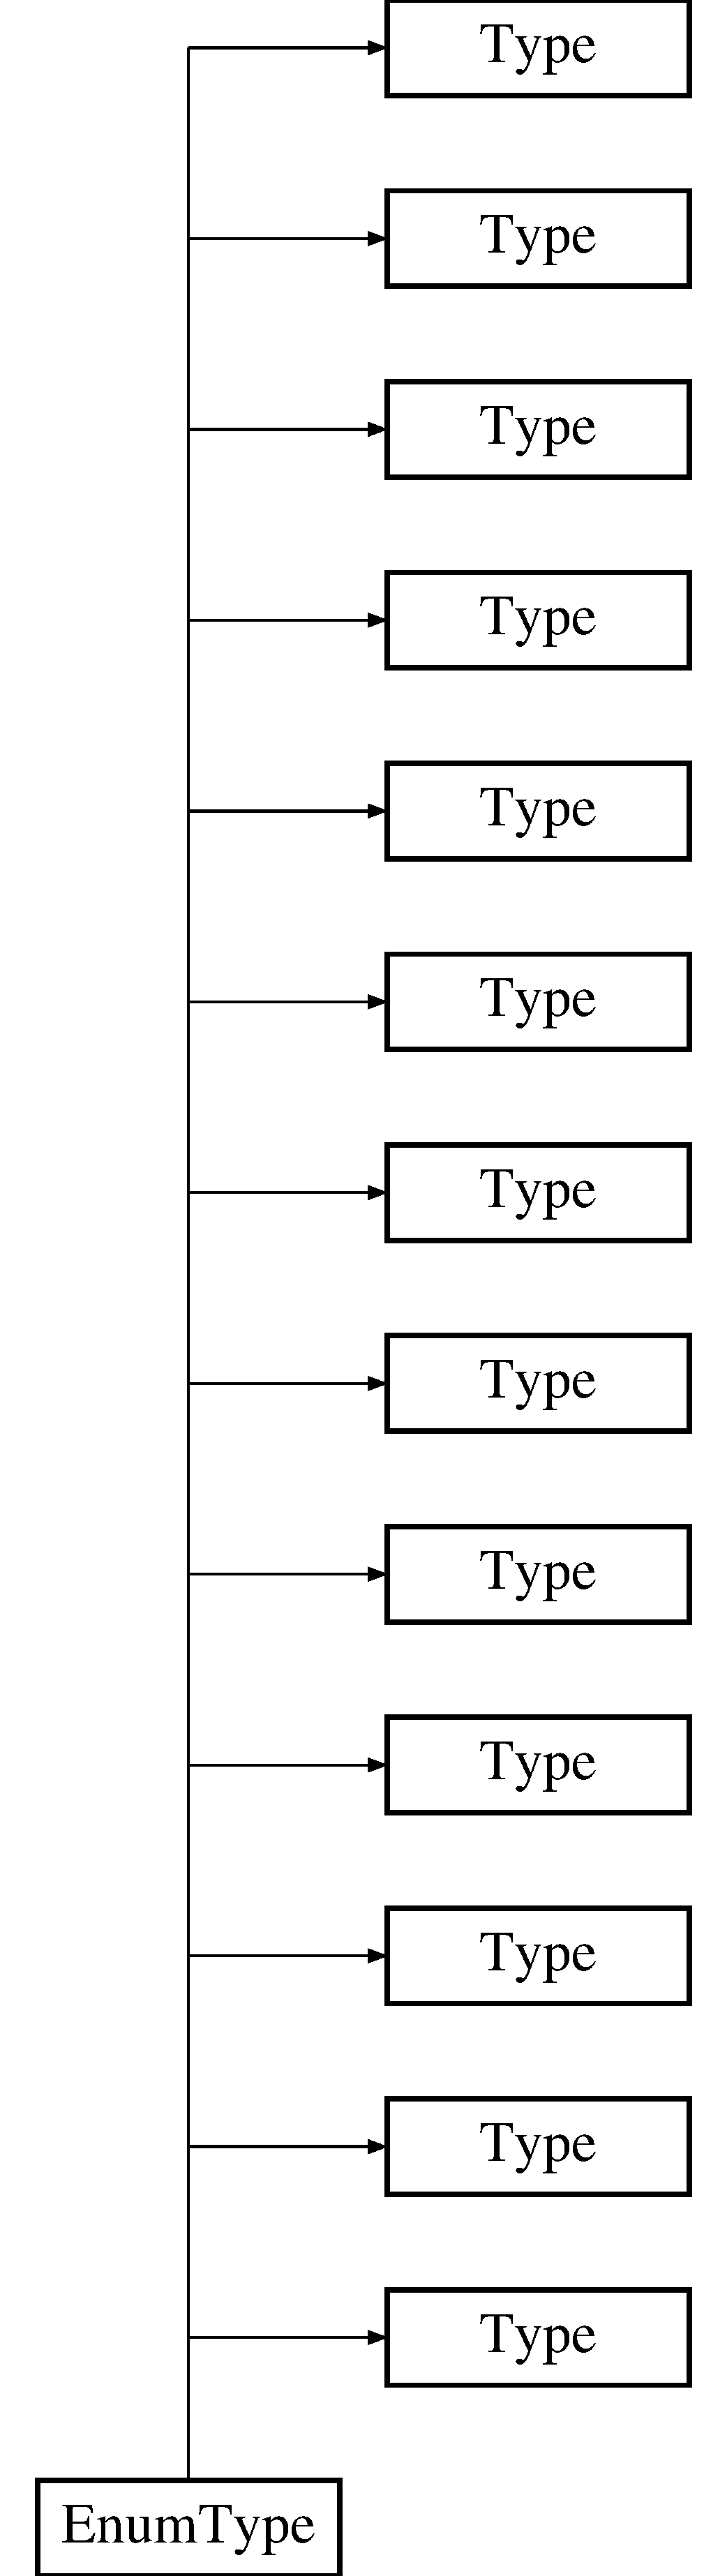
\includegraphics[height=2.000000cm]{classEnumType}
\end{center}
\end{figure}
\subsection*{Public Member Functions}
\begin{DoxyCompactItemize}
\item 
\hypertarget{classEnumType_ae7c41f665f312e82e0c50614726ef6e1}{{\bfseries Enum\-Type} (string n, int start\-Val)}\label{classEnumType_ae7c41f665f312e82e0c50614726ef6e1}

\item 
\hypertarget{classEnumType_a4011034b4e53b36addbefbcf1bf93121}{int {\bfseries Get\-Const\-Val} (string s)}\label{classEnumType_a4011034b4e53b36addbefbcf1bf93121}

\item 
\hypertarget{classEnumType_aeebf9ff85428ac5804ba7939c8c227e7}{void {\bfseries Add\-Enum\-Const} (string s)}\label{classEnumType_aeebf9ff85428ac5804ba7939c8c227e7}

\item 
\hypertarget{classEnumType_a161ca3b2bbad063c616813f0cfb23812}{void {\bfseries Add\-Enum\-Const} (string s, int val)}\label{classEnumType_a161ca3b2bbad063c616813f0cfb23812}

\item 
\hypertarget{classType_a8143fe4686ae1a5709a5955396c6ee26}{string {\bfseries Get\-Name} ()}\label{classType_a8143fe4686ae1a5709a5955396c6ee26}

\item 
\hypertarget{classType_afe0fca035825759785b525d2a24f69fe}{int {\bfseries Get\-Size} ()}\label{classType_afe0fca035825759785b525d2a24f69fe}

\item 
\hypertarget{classType_ab8d2328a3a76289edf42b9bf0d4f278f}{void {\bfseries Set\-Name} (string n)}\label{classType_ab8d2328a3a76289edf42b9bf0d4f278f}

\end{DoxyCompactItemize}
\subsection*{Protected Attributes}
\begin{DoxyCompactItemize}
\item 
\hypertarget{classEnumType_ae294fba1687454c3f28825ab29031184}{map$<$ string, int $>$ {\bfseries enum\-Consts}}\label{classEnumType_ae294fba1687454c3f28825ab29031184}

\item 
\hypertarget{classEnumType_ac46ec8a6259d6c946716d89103125f89}{int {\bfseries current\-Val}}\label{classEnumType_ac46ec8a6259d6c946716d89103125f89}

\item 
\hypertarget{classType_ad7eeefba3dfcecbdaa98d46aaa84e389}{string {\bfseries name}}\label{classType_ad7eeefba3dfcecbdaa98d46aaa84e389}

\item 
\hypertarget{classType_a871302dc63ac1a37c0b6a225cf82048d}{int {\bfseries size}}\label{classType_a871302dc63ac1a37c0b6a225cf82048d}

\end{DoxyCompactItemize}


The documentation for this class was generated from the following files\-:\begin{DoxyCompactItemize}
\item 
Type.\-h\item 
Type.\-cpp\end{DoxyCompactItemize}

\input{classGoFPatterns_1_1Event}
\input{structFunction}
\input{classFunctionTable}
\hypertarget{classFunctionType}{\section{Function\-Type Class Reference}
\label{classFunctionType}\index{Function\-Type@{Function\-Type}}
}
Inheritance diagram for Function\-Type\-:\begin{figure}[H]
\begin{center}
\leavevmode
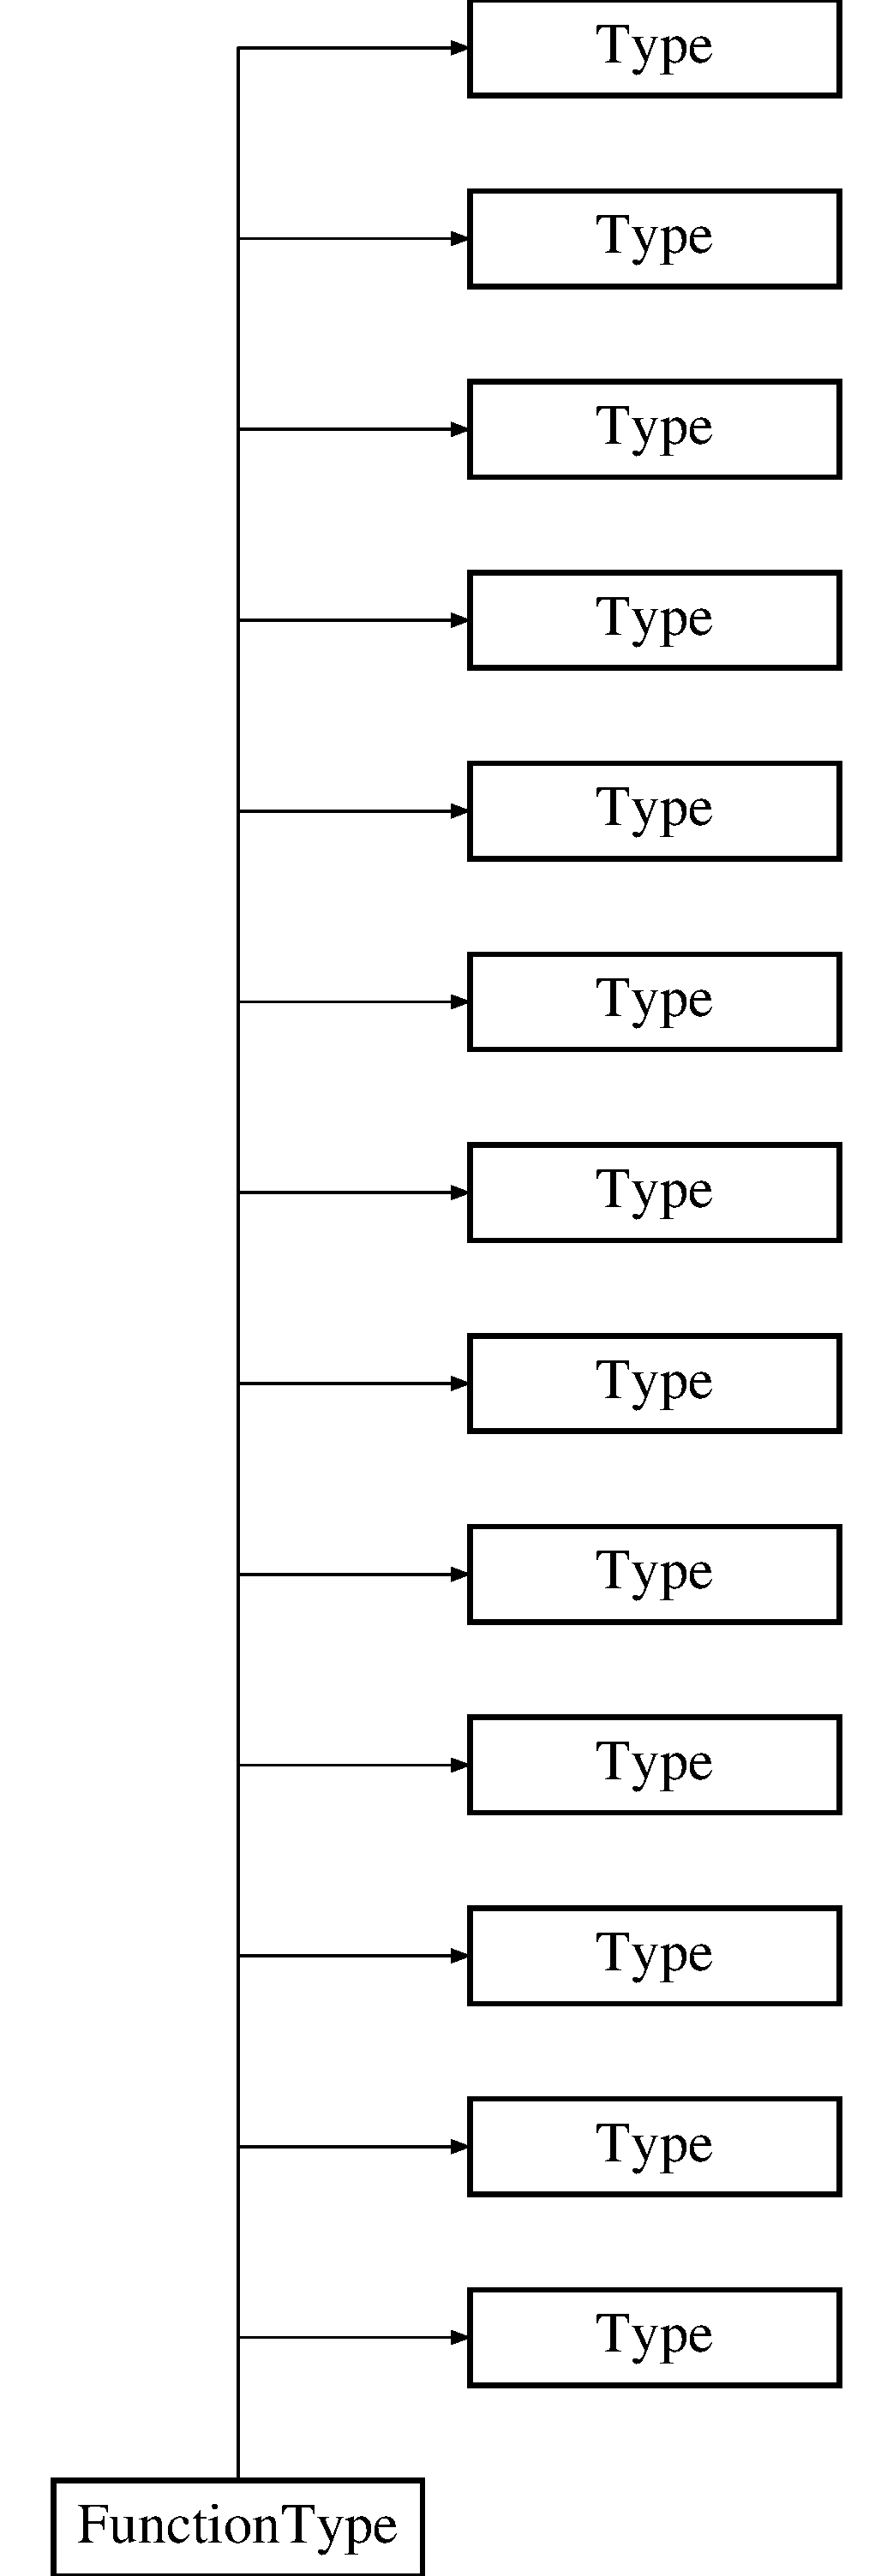
\includegraphics[height=2.000000cm]{classFunctionType}
\end{center}
\end{figure}
\subsection*{Public Member Functions}
\begin{DoxyCompactItemize}
\item 
\hypertarget{classFunctionType_a924981ea6fc18a7a9ed4cb5c94a136d6}{{\bfseries Function\-Type} (string n)}\label{classFunctionType_a924981ea6fc18a7a9ed4cb5c94a136d6}

\item 
\hypertarget{classFunctionType_a9259c94250b6cb903c6013bc10a0b7bc}{void {\bfseries Add\-Param} (\hyperlink{classType}{Type} $\ast$t)}\label{classFunctionType_a9259c94250b6cb903c6013bc10a0b7bc}

\item 
\hypertarget{classFunctionType_a1462775c5732b70b07c689ab7088814d}{void {\bfseries Set\-Return\-Type} (\hyperlink{classType}{Type} $\ast$t)}\label{classFunctionType_a1462775c5732b70b07c689ab7088814d}

\item 
\hypertarget{classFunctionType_a8b6fed7ff4d79b5db3d39cd042326090}{int {\bfseries Get\-Param\-Count} ()}\label{classFunctionType_a8b6fed7ff4d79b5db3d39cd042326090}

\item 
\hypertarget{classFunctionType_a601e763553086c0d7a4c2de97d6de2bc}{\hyperlink{classType}{Type} $\ast$ {\bfseries Get\-Return\-Type} ()}\label{classFunctionType_a601e763553086c0d7a4c2de97d6de2bc}

\item 
\hypertarget{classType_a8143fe4686ae1a5709a5955396c6ee26}{string {\bfseries Get\-Name} ()}\label{classType_a8143fe4686ae1a5709a5955396c6ee26}

\item 
\hypertarget{classType_afe0fca035825759785b525d2a24f69fe}{int {\bfseries Get\-Size} ()}\label{classType_afe0fca035825759785b525d2a24f69fe}

\item 
\hypertarget{classType_ab8d2328a3a76289edf42b9bf0d4f278f}{void {\bfseries Set\-Name} (string n)}\label{classType_ab8d2328a3a76289edf42b9bf0d4f278f}

\end{DoxyCompactItemize}
\subsection*{Protected Attributes}
\begin{DoxyCompactItemize}
\item 
\hypertarget{classFunctionType_a83a13121b4be94af8ca95104030e7873}{vector$<$ \hyperlink{classType}{Type} $\ast$ $>$ {\bfseries params}}\label{classFunctionType_a83a13121b4be94af8ca95104030e7873}

\item 
\hypertarget{classFunctionType_a4512eaeaafe53ef9056acd3314263aaa}{\hyperlink{classType}{Type} $\ast$ {\bfseries return\-Type}}\label{classFunctionType_a4512eaeaafe53ef9056acd3314263aaa}

\item 
\hypertarget{classType_ad7eeefba3dfcecbdaa98d46aaa84e389}{string {\bfseries name}}\label{classType_ad7eeefba3dfcecbdaa98d46aaa84e389}

\item 
\hypertarget{classType_a871302dc63ac1a37c0b6a225cf82048d}{int {\bfseries size}}\label{classType_a871302dc63ac1a37c0b6a225cf82048d}

\end{DoxyCompactItemize}


The documentation for this class was generated from the following files\-:\begin{DoxyCompactItemize}
\item 
Type.\-h\item 
Type.\-cpp\end{DoxyCompactItemize}

\hypertarget{structInputLine}{\section{Input\-Line Struct Reference}
\label{structInputLine}\index{Input\-Line@{Input\-Line}}
}
\subsection*{Public Member Functions}
\begin{DoxyCompactItemize}
\item 
\hypertarget{structInputLine_a6a57eafd6e53ea99651327e174c52077}{{\bfseries Input\-Line} (int l, string s)}\label{structInputLine_a6a57eafd6e53ea99651327e174c52077}

\end{DoxyCompactItemize}
\subsection*{Public Attributes}
\begin{DoxyCompactItemize}
\item 
\hypertarget{structInputLine_aef26343331dc90be48f6fdbf4ab85276}{int {\bfseries line}}\label{structInputLine_aef26343331dc90be48f6fdbf4ab85276}

\item 
\hypertarget{structInputLine_aa448799cf6fd6735d55c2cadb394e16f}{string {\bfseries text}}\label{structInputLine_aa448799cf6fd6735d55c2cadb394e16f}

\end{DoxyCompactItemize}


The documentation for this struct was generated from the following file\-:\begin{DoxyCompactItemize}
\item 
C\-Compiler.\-h\end{DoxyCompactItemize}

\hypertarget{structAVLTree_1_1Node}{\section{A\-V\-L\-Tree$<$ Data\-Item $>$\-:\-:Node Struct Reference}
\label{structAVLTree_1_1Node}\index{A\-V\-L\-Tree$<$ Data\-Item $>$\-::\-Node@{A\-V\-L\-Tree$<$ Data\-Item $>$\-::\-Node}}
}


A node which composes the Data\-Item template class with pointers to its children nodes in the A\-V\-L tree and the balance factor at the current node.  


\subsection*{Public Attributes}
\begin{DoxyCompactItemize}
\item 
\hypertarget{structAVLTree_1_1Node_a7be4bf3468896388ac4ca7927efa5309}{Data\-Item {\bfseries data}}\label{structAVLTree_1_1Node_a7be4bf3468896388ac4ca7927efa5309}

\item 
\hypertarget{structAVLTree_1_1Node_a8be0751ba22e265f286feb85488a6faa}{\hyperlink{structAVLTree_1_1Node}{Node} $\ast$ {\bfseries children} \mbox{[}C\-H\-I\-L\-D\-\_\-\-S\-I\-Z\-E\mbox{]}}\label{structAVLTree_1_1Node_a8be0751ba22e265f286feb85488a6faa}

\item 
\hypertarget{structAVLTree_1_1Node_a0ac3a6b042130f476df783d77c350915}{int {\bfseries balance\-Factor}}\label{structAVLTree_1_1Node_a0ac3a6b042130f476df783d77c350915}

\end{DoxyCompactItemize}


\subsection{Detailed Description}
\subsubsection*{template$<$class Data\-Item$>$struct A\-V\-L\-Tree$<$ Data\-Item $>$\-::\-Node}

A node which composes the Data\-Item template class with pointers to its children nodes in the A\-V\-L tree and the balance factor at the current node. 

The documentation for this struct was generated from the following file\-:\begin{DoxyCompactItemize}
\item 
Avl\-Tree.\-h\end{DoxyCompactItemize}

\input{structParameter}
\hypertarget{classPODType}{\section{P\-O\-D\-Type Class Reference}
\label{classPODType}\index{P\-O\-D\-Type@{P\-O\-D\-Type}}
}
Inheritance diagram for P\-O\-D\-Type\-:\begin{figure}[H]
\begin{center}
\leavevmode
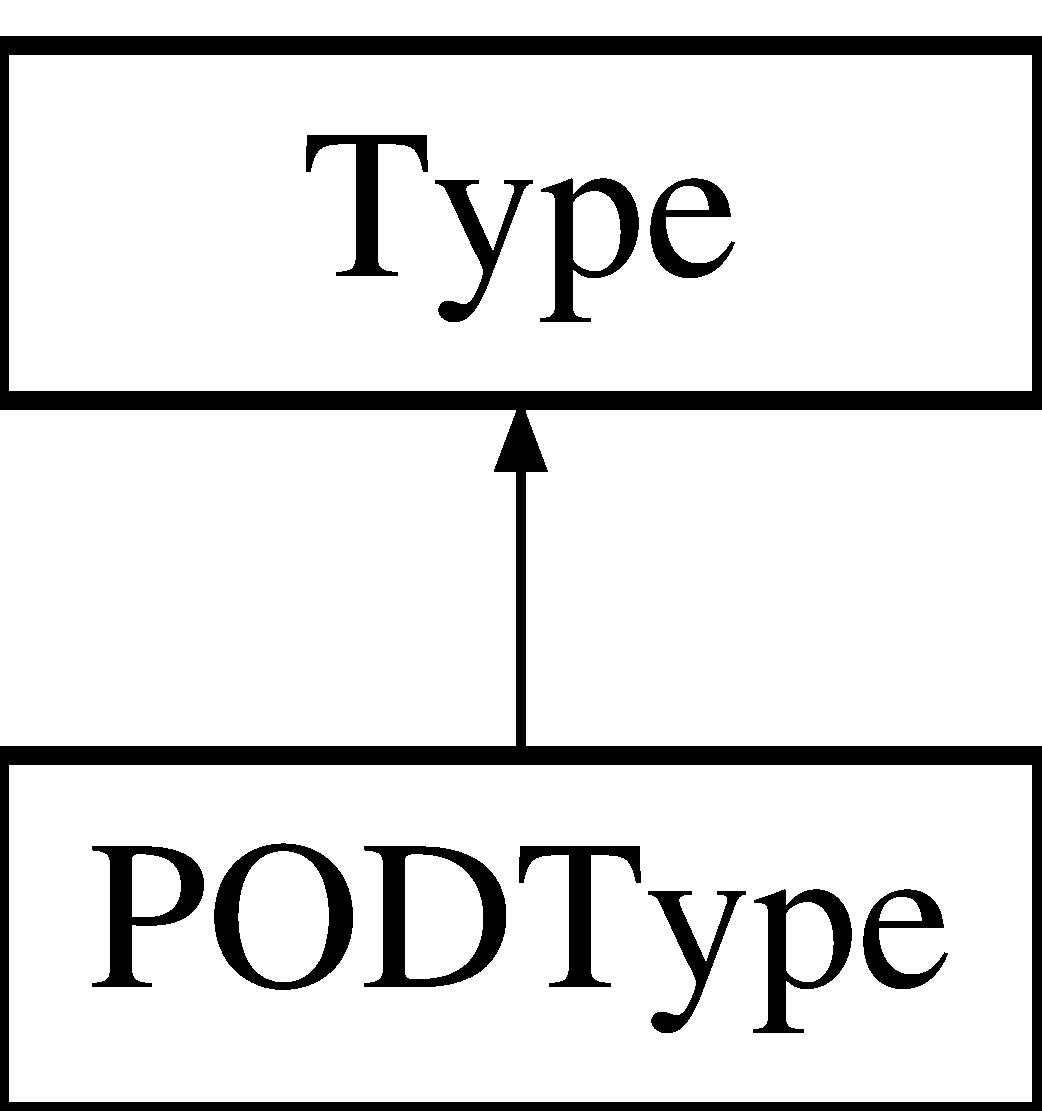
\includegraphics[height=2.000000cm]{classPODType}
\end{center}
\end{figure}
\subsection*{Public Member Functions}
\begin{DoxyCompactItemize}
\item 
\hypertarget{classPODType_a386ded726d22fbd62f3a2b49d8a29a6f}{{\bfseries P\-O\-D\-Type} (string n, int s)}\label{classPODType_a386ded726d22fbd62f3a2b49d8a29a6f}

\item 
\hypertarget{classPODType_ac64782a9fa6ecff753f4b59535ff8303}{bool {\bfseries is\-Signed} ()}\label{classPODType_ac64782a9fa6ecff753f4b59535ff8303}

\item 
\hypertarget{classPODType_ab76d7be88f388fadc10a0c34f3e576e8}{void {\bfseries Set\-Signed} (bool is\-Signed)}\label{classPODType_ab76d7be88f388fadc10a0c34f3e576e8}

\item 
\hypertarget{classType_a8143fe4686ae1a5709a5955396c6ee26}{string {\bfseries Get\-Name} ()}\label{classType_a8143fe4686ae1a5709a5955396c6ee26}

\item 
\hypertarget{classType_afe0fca035825759785b525d2a24f69fe}{int {\bfseries Get\-Size} ()}\label{classType_afe0fca035825759785b525d2a24f69fe}

\item 
\hypertarget{classType_ab8d2328a3a76289edf42b9bf0d4f278f}{void {\bfseries Set\-Name} (string n)}\label{classType_ab8d2328a3a76289edf42b9bf0d4f278f}

\end{DoxyCompactItemize}
\subsection*{Protected Attributes}
\begin{DoxyCompactItemize}
\item 
\hypertarget{classPODType_a70fc6860646131aa3bad5800257522b5}{bool {\bfseries is\-\_\-signed}}\label{classPODType_a70fc6860646131aa3bad5800257522b5}

\item 
\hypertarget{classType_ad7eeefba3dfcecbdaa98d46aaa84e389}{string {\bfseries name}}\label{classType_ad7eeefba3dfcecbdaa98d46aaa84e389}

\item 
\hypertarget{classType_a871302dc63ac1a37c0b6a225cf82048d}{int {\bfseries size}}\label{classType_a871302dc63ac1a37c0b6a225cf82048d}

\end{DoxyCompactItemize}


The documentation for this class was generated from the following files\-:\begin{DoxyCompactItemize}
\item 
Type.\-h\item 
Type.\-cpp\end{DoxyCompactItemize}

\hypertarget{classPointerType}{\section{Pointer\-Type Class Reference}
\label{classPointerType}\index{Pointer\-Type@{Pointer\-Type}}
}
Inheritance diagram for Pointer\-Type\-:\begin{figure}[H]
\begin{center}
\leavevmode
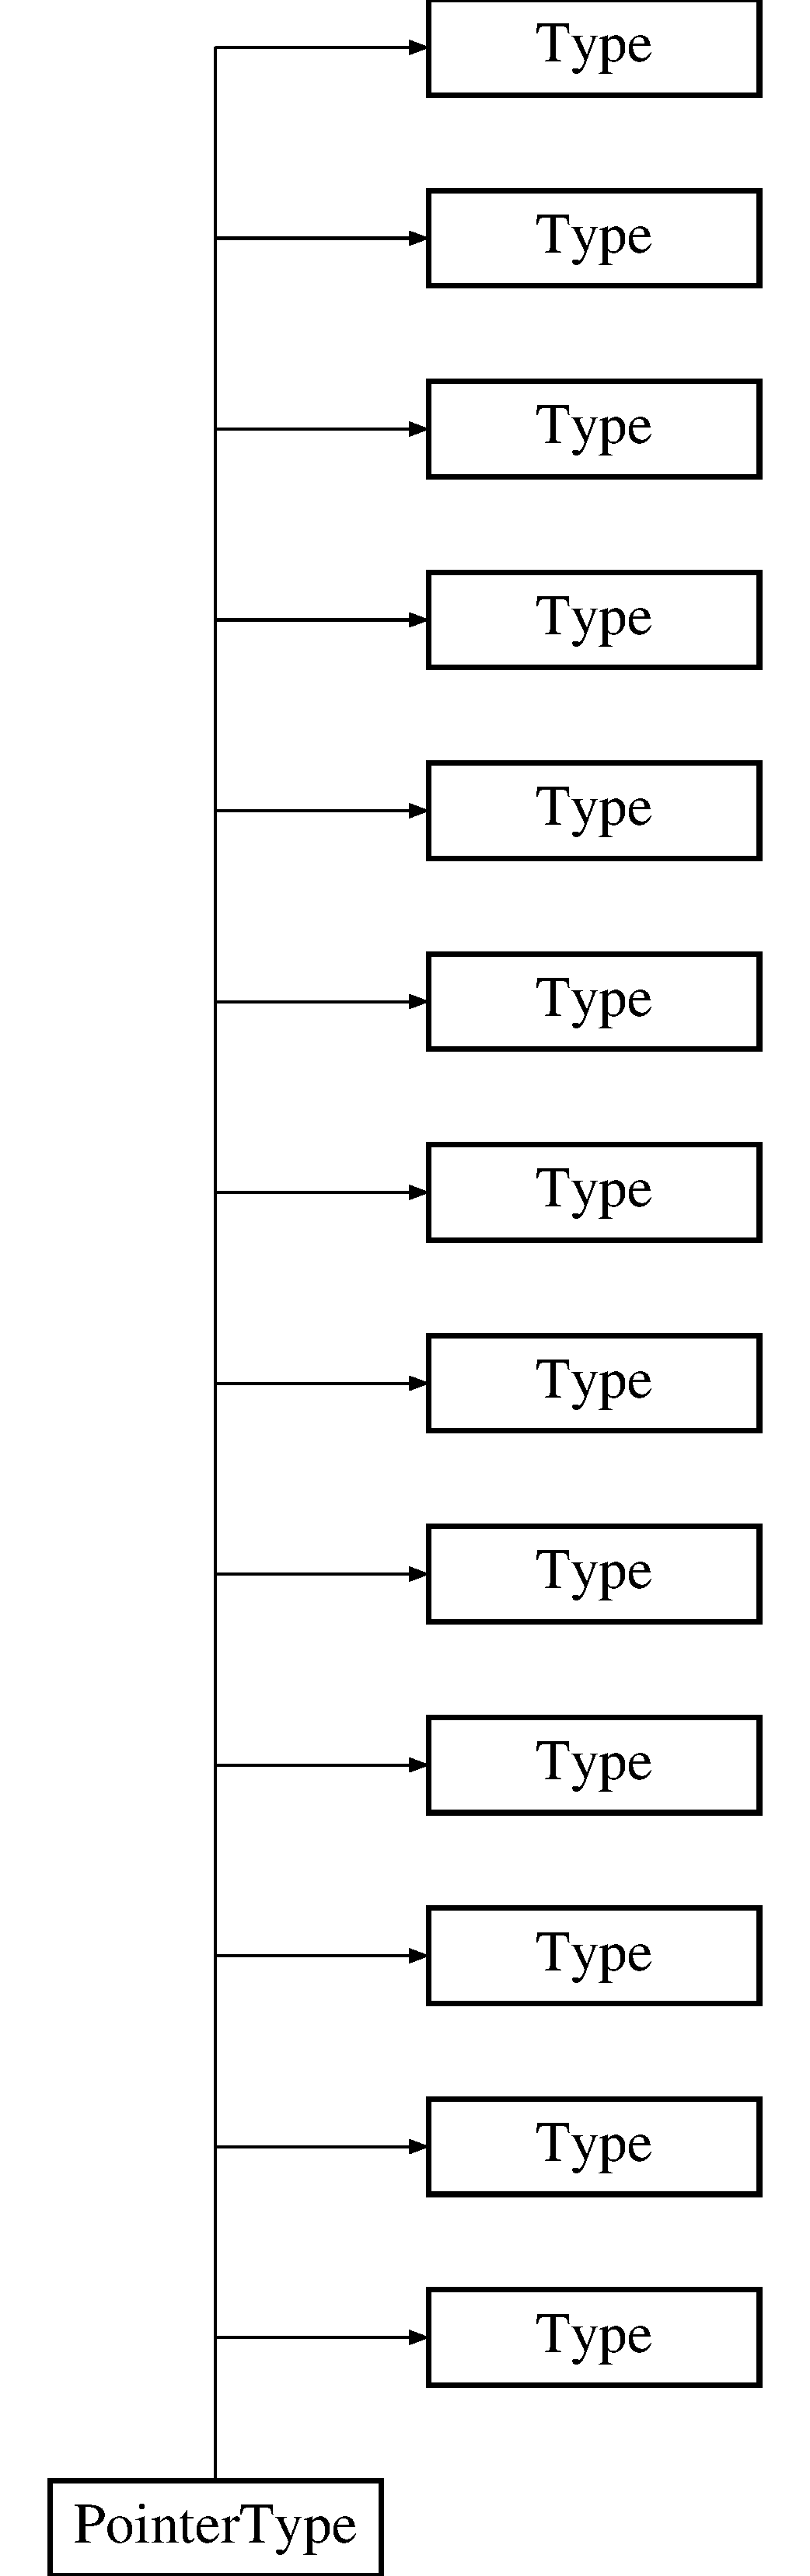
\includegraphics[height=12.000000cm]{classPointerType}
\end{center}
\end{figure}
\subsection*{Public Types}
\begin{DoxyCompactItemize}
\item 
enum {\bfseries Derived\-Type} \{ \\*
{\bfseries B\-A\-S\-E}, 
{\bfseries P\-O\-D\-T\-Y\-P\-E}, 
{\bfseries T\-Y\-P\-E\-D\-E\-F\-T\-Y\-P\-E}, 
{\bfseries E\-N\-U\-M\-T\-Y\-P\-E}, 
\\*
{\bfseries A\-R\-R\-A\-Y\-T\-Y\-P\-E}, 
{\bfseries S\-T\-R\-U\-C\-T\-T\-Y\-P\-E}, 
{\bfseries U\-N\-I\-O\-N\-T\-Y\-P\-E}, 
{\bfseries F\-U\-N\-C\-T\-I\-O\-N\-T\-Y\-P\-E}, 
\\*
{\bfseries P\-O\-I\-N\-T\-E\-R\-T\-Y\-P\-E}, 
{\bfseries B\-A\-S\-E}, 
{\bfseries P\-O\-D\-T\-Y\-P\-E}, 
{\bfseries T\-Y\-P\-E\-D\-E\-F\-T\-Y\-P\-E}, 
\\*
{\bfseries E\-N\-U\-M\-T\-Y\-P\-E}, 
{\bfseries A\-R\-R\-A\-Y\-T\-Y\-P\-E}, 
{\bfseries S\-T\-R\-U\-C\-T\-T\-Y\-P\-E}, 
{\bfseries U\-N\-I\-O\-N\-T\-Y\-P\-E}, 
\\*
{\bfseries F\-U\-N\-C\-T\-I\-O\-N\-T\-Y\-P\-E}, 
{\bfseries P\-O\-I\-N\-T\-E\-R\-T\-Y\-P\-E}, 
{\bfseries B\-A\-S\-E}, 
{\bfseries P\-O\-D\-T\-Y\-P\-E}, 
\\*
{\bfseries T\-Y\-P\-E\-D\-E\-F\-T\-Y\-P\-E}, 
{\bfseries E\-N\-U\-M\-T\-Y\-P\-E}, 
{\bfseries A\-R\-R\-A\-Y\-T\-Y\-P\-E}, 
{\bfseries S\-T\-R\-U\-C\-T\-T\-Y\-P\-E}, 
\\*
{\bfseries U\-N\-I\-O\-N\-T\-Y\-P\-E}, 
{\bfseries F\-U\-N\-C\-T\-I\-O\-N\-T\-Y\-P\-E}, 
{\bfseries P\-O\-I\-N\-T\-E\-R\-T\-Y\-P\-E}, 
{\bfseries B\-A\-S\-E}, 
\\*
{\bfseries P\-O\-D\-T\-Y\-P\-E}, 
{\bfseries T\-Y\-P\-E\-D\-E\-F\-T\-Y\-P\-E}, 
{\bfseries E\-N\-U\-M\-T\-Y\-P\-E}, 
{\bfseries A\-R\-R\-A\-Y\-T\-Y\-P\-E}, 
\\*
{\bfseries S\-T\-R\-U\-C\-T\-T\-Y\-P\-E}, 
{\bfseries U\-N\-I\-O\-N\-T\-Y\-P\-E}, 
{\bfseries F\-U\-N\-C\-T\-I\-O\-N\-T\-Y\-P\-E}, 
{\bfseries P\-O\-I\-N\-T\-E\-R\-T\-Y\-P\-E}, 
\\*
{\bfseries B\-A\-S\-E}, 
{\bfseries P\-O\-D\-T\-Y\-P\-E}, 
{\bfseries T\-Y\-P\-E\-D\-E\-F\-T\-Y\-P\-E}, 
{\bfseries E\-N\-U\-M\-T\-Y\-P\-E}, 
\\*
{\bfseries A\-R\-R\-A\-Y\-T\-Y\-P\-E}, 
{\bfseries S\-T\-R\-U\-C\-T\-T\-Y\-P\-E}, 
{\bfseries U\-N\-I\-O\-N\-T\-Y\-P\-E}, 
{\bfseries F\-U\-N\-C\-T\-I\-O\-N\-T\-Y\-P\-E}, 
\\*
{\bfseries P\-O\-I\-N\-T\-E\-R\-T\-Y\-P\-E}, 
{\bfseries B\-A\-S\-E}, 
{\bfseries P\-O\-D\-T\-Y\-P\-E}, 
{\bfseries T\-Y\-P\-E\-D\-E\-F\-T\-Y\-P\-E}, 
\\*
{\bfseries E\-N\-U\-M\-T\-Y\-P\-E}, 
{\bfseries A\-R\-R\-A\-Y\-T\-Y\-P\-E}, 
{\bfseries S\-T\-R\-U\-C\-T\-T\-Y\-P\-E}, 
{\bfseries U\-N\-I\-O\-N\-T\-Y\-P\-E}, 
\\*
{\bfseries F\-U\-N\-C\-T\-I\-O\-N\-T\-Y\-P\-E}, 
{\bfseries P\-O\-I\-N\-T\-E\-R\-T\-Y\-P\-E}, 
{\bfseries B\-A\-S\-E}, 
{\bfseries P\-O\-D\-T\-Y\-P\-E}, 
\\*
{\bfseries T\-Y\-P\-E\-D\-E\-F\-T\-Y\-P\-E}, 
{\bfseries E\-N\-U\-M\-T\-Y\-P\-E}, 
{\bfseries A\-R\-R\-A\-Y\-T\-Y\-P\-E}, 
{\bfseries S\-T\-R\-U\-C\-T\-T\-Y\-P\-E}, 
\\*
{\bfseries U\-N\-I\-O\-N\-T\-Y\-P\-E}, 
{\bfseries F\-U\-N\-C\-T\-I\-O\-N\-T\-Y\-P\-E}, 
{\bfseries P\-O\-I\-N\-T\-E\-R\-T\-Y\-P\-E}, 
{\bfseries B\-A\-S\-E}, 
\\*
{\bfseries P\-O\-D\-T\-Y\-P\-E}, 
{\bfseries T\-Y\-P\-E\-D\-E\-F\-T\-Y\-P\-E}, 
{\bfseries E\-N\-U\-M\-T\-Y\-P\-E}, 
{\bfseries A\-R\-R\-A\-Y\-T\-Y\-P\-E}, 
\\*
{\bfseries S\-T\-R\-U\-C\-T\-T\-Y\-P\-E}, 
{\bfseries U\-N\-I\-O\-N\-T\-Y\-P\-E}, 
{\bfseries F\-U\-N\-C\-T\-I\-O\-N\-T\-Y\-P\-E}, 
{\bfseries P\-O\-I\-N\-T\-E\-R\-T\-Y\-P\-E}, 
\\*
{\bfseries B\-A\-S\-E}, 
{\bfseries P\-O\-D\-T\-Y\-P\-E}, 
{\bfseries T\-Y\-P\-E\-D\-E\-F\-T\-Y\-P\-E}, 
{\bfseries E\-N\-U\-M\-T\-Y\-P\-E}, 
\\*
{\bfseries A\-R\-R\-A\-Y\-T\-Y\-P\-E}, 
{\bfseries S\-T\-R\-U\-C\-T\-T\-Y\-P\-E}, 
{\bfseries U\-N\-I\-O\-N\-T\-Y\-P\-E}, 
{\bfseries F\-U\-N\-C\-T\-I\-O\-N\-T\-Y\-P\-E}, 
\\*
{\bfseries P\-O\-I\-N\-T\-E\-R\-T\-Y\-P\-E}, 
{\bfseries B\-A\-S\-E}, 
{\bfseries P\-O\-D\-T\-Y\-P\-E}, 
{\bfseries T\-Y\-P\-E\-D\-E\-F\-T\-Y\-P\-E}, 
\\*
{\bfseries E\-N\-U\-M\-T\-Y\-P\-E}, 
{\bfseries A\-R\-R\-A\-Y\-T\-Y\-P\-E}, 
{\bfseries S\-T\-R\-U\-C\-T\-T\-Y\-P\-E}, 
{\bfseries U\-N\-I\-O\-N\-T\-Y\-P\-E}, 
\\*
{\bfseries F\-U\-N\-C\-T\-I\-O\-N\-T\-Y\-P\-E}, 
{\bfseries P\-O\-I\-N\-T\-E\-R\-T\-Y\-P\-E}, 
{\bfseries B\-A\-S\-E}, 
{\bfseries P\-O\-D\-T\-Y\-P\-E}, 
\\*
{\bfseries T\-Y\-P\-E\-D\-E\-F\-T\-Y\-P\-E}, 
{\bfseries E\-N\-U\-M\-T\-Y\-P\-E}, 
{\bfseries A\-R\-R\-A\-Y\-T\-Y\-P\-E}, 
{\bfseries S\-T\-R\-U\-C\-T\-T\-Y\-P\-E}, 
\\*
{\bfseries U\-N\-I\-O\-N\-T\-Y\-P\-E}, 
{\bfseries F\-U\-N\-C\-T\-I\-O\-N\-T\-Y\-P\-E}, 
{\bfseries P\-O\-I\-N\-T\-E\-R\-T\-Y\-P\-E}, 
{\bfseries B\-A\-S\-E}, 
\\*
{\bfseries P\-O\-D\-T\-Y\-P\-E}, 
{\bfseries T\-Y\-P\-E\-D\-E\-F\-T\-Y\-P\-E}, 
{\bfseries E\-N\-U\-M\-T\-Y\-P\-E}, 
{\bfseries A\-R\-R\-A\-Y\-T\-Y\-P\-E}, 
\\*
{\bfseries S\-T\-R\-U\-C\-T\-T\-Y\-P\-E}, 
{\bfseries U\-N\-I\-O\-N\-T\-Y\-P\-E}, 
{\bfseries F\-U\-N\-C\-T\-I\-O\-N\-T\-Y\-P\-E}, 
{\bfseries P\-O\-I\-N\-T\-E\-R\-T\-Y\-P\-E}, 
\\*
{\bfseries B\-A\-S\-E}, 
{\bfseries P\-O\-D\-T\-Y\-P\-E}, 
{\bfseries T\-Y\-P\-E\-D\-E\-F\-T\-Y\-P\-E}, 
{\bfseries E\-N\-U\-M\-T\-Y\-P\-E}, 
\\*
{\bfseries A\-R\-R\-A\-Y\-T\-Y\-P\-E}, 
{\bfseries S\-T\-R\-U\-C\-T\-T\-Y\-P\-E}, 
{\bfseries U\-N\-I\-O\-N\-T\-Y\-P\-E}, 
{\bfseries F\-U\-N\-C\-T\-I\-O\-N\-T\-Y\-P\-E}, 
\\*
{\bfseries P\-O\-I\-N\-T\-E\-R\-T\-Y\-P\-E}
 \}
\item 
enum {\bfseries Derived\-Type} \{ \\*
{\bfseries B\-A\-S\-E}, 
{\bfseries P\-O\-D\-T\-Y\-P\-E}, 
{\bfseries T\-Y\-P\-E\-D\-E\-F\-T\-Y\-P\-E}, 
{\bfseries E\-N\-U\-M\-T\-Y\-P\-E}, 
\\*
{\bfseries A\-R\-R\-A\-Y\-T\-Y\-P\-E}, 
{\bfseries S\-T\-R\-U\-C\-T\-T\-Y\-P\-E}, 
{\bfseries U\-N\-I\-O\-N\-T\-Y\-P\-E}, 
{\bfseries F\-U\-N\-C\-T\-I\-O\-N\-T\-Y\-P\-E}, 
\\*
{\bfseries P\-O\-I\-N\-T\-E\-R\-T\-Y\-P\-E}, 
{\bfseries B\-A\-S\-E}, 
{\bfseries P\-O\-D\-T\-Y\-P\-E}, 
{\bfseries T\-Y\-P\-E\-D\-E\-F\-T\-Y\-P\-E}, 
\\*
{\bfseries E\-N\-U\-M\-T\-Y\-P\-E}, 
{\bfseries A\-R\-R\-A\-Y\-T\-Y\-P\-E}, 
{\bfseries S\-T\-R\-U\-C\-T\-T\-Y\-P\-E}, 
{\bfseries U\-N\-I\-O\-N\-T\-Y\-P\-E}, 
\\*
{\bfseries F\-U\-N\-C\-T\-I\-O\-N\-T\-Y\-P\-E}, 
{\bfseries P\-O\-I\-N\-T\-E\-R\-T\-Y\-P\-E}, 
{\bfseries B\-A\-S\-E}, 
{\bfseries P\-O\-D\-T\-Y\-P\-E}, 
\\*
{\bfseries T\-Y\-P\-E\-D\-E\-F\-T\-Y\-P\-E}, 
{\bfseries E\-N\-U\-M\-T\-Y\-P\-E}, 
{\bfseries A\-R\-R\-A\-Y\-T\-Y\-P\-E}, 
{\bfseries S\-T\-R\-U\-C\-T\-T\-Y\-P\-E}, 
\\*
{\bfseries U\-N\-I\-O\-N\-T\-Y\-P\-E}, 
{\bfseries F\-U\-N\-C\-T\-I\-O\-N\-T\-Y\-P\-E}, 
{\bfseries P\-O\-I\-N\-T\-E\-R\-T\-Y\-P\-E}, 
{\bfseries B\-A\-S\-E}, 
\\*
{\bfseries P\-O\-D\-T\-Y\-P\-E}, 
{\bfseries T\-Y\-P\-E\-D\-E\-F\-T\-Y\-P\-E}, 
{\bfseries E\-N\-U\-M\-T\-Y\-P\-E}, 
{\bfseries A\-R\-R\-A\-Y\-T\-Y\-P\-E}, 
\\*
{\bfseries S\-T\-R\-U\-C\-T\-T\-Y\-P\-E}, 
{\bfseries U\-N\-I\-O\-N\-T\-Y\-P\-E}, 
{\bfseries F\-U\-N\-C\-T\-I\-O\-N\-T\-Y\-P\-E}, 
{\bfseries P\-O\-I\-N\-T\-E\-R\-T\-Y\-P\-E}, 
\\*
{\bfseries B\-A\-S\-E}, 
{\bfseries P\-O\-D\-T\-Y\-P\-E}, 
{\bfseries T\-Y\-P\-E\-D\-E\-F\-T\-Y\-P\-E}, 
{\bfseries E\-N\-U\-M\-T\-Y\-P\-E}, 
\\*
{\bfseries A\-R\-R\-A\-Y\-T\-Y\-P\-E}, 
{\bfseries S\-T\-R\-U\-C\-T\-T\-Y\-P\-E}, 
{\bfseries U\-N\-I\-O\-N\-T\-Y\-P\-E}, 
{\bfseries F\-U\-N\-C\-T\-I\-O\-N\-T\-Y\-P\-E}, 
\\*
{\bfseries P\-O\-I\-N\-T\-E\-R\-T\-Y\-P\-E}, 
{\bfseries B\-A\-S\-E}, 
{\bfseries P\-O\-D\-T\-Y\-P\-E}, 
{\bfseries T\-Y\-P\-E\-D\-E\-F\-T\-Y\-P\-E}, 
\\*
{\bfseries E\-N\-U\-M\-T\-Y\-P\-E}, 
{\bfseries A\-R\-R\-A\-Y\-T\-Y\-P\-E}, 
{\bfseries S\-T\-R\-U\-C\-T\-T\-Y\-P\-E}, 
{\bfseries U\-N\-I\-O\-N\-T\-Y\-P\-E}, 
\\*
{\bfseries F\-U\-N\-C\-T\-I\-O\-N\-T\-Y\-P\-E}, 
{\bfseries P\-O\-I\-N\-T\-E\-R\-T\-Y\-P\-E}, 
{\bfseries B\-A\-S\-E}, 
{\bfseries P\-O\-D\-T\-Y\-P\-E}, 
\\*
{\bfseries T\-Y\-P\-E\-D\-E\-F\-T\-Y\-P\-E}, 
{\bfseries E\-N\-U\-M\-T\-Y\-P\-E}, 
{\bfseries A\-R\-R\-A\-Y\-T\-Y\-P\-E}, 
{\bfseries S\-T\-R\-U\-C\-T\-T\-Y\-P\-E}, 
\\*
{\bfseries U\-N\-I\-O\-N\-T\-Y\-P\-E}, 
{\bfseries F\-U\-N\-C\-T\-I\-O\-N\-T\-Y\-P\-E}, 
{\bfseries P\-O\-I\-N\-T\-E\-R\-T\-Y\-P\-E}, 
{\bfseries B\-A\-S\-E}, 
\\*
{\bfseries P\-O\-D\-T\-Y\-P\-E}, 
{\bfseries T\-Y\-P\-E\-D\-E\-F\-T\-Y\-P\-E}, 
{\bfseries E\-N\-U\-M\-T\-Y\-P\-E}, 
{\bfseries A\-R\-R\-A\-Y\-T\-Y\-P\-E}, 
\\*
{\bfseries S\-T\-R\-U\-C\-T\-T\-Y\-P\-E}, 
{\bfseries U\-N\-I\-O\-N\-T\-Y\-P\-E}, 
{\bfseries F\-U\-N\-C\-T\-I\-O\-N\-T\-Y\-P\-E}, 
{\bfseries P\-O\-I\-N\-T\-E\-R\-T\-Y\-P\-E}, 
\\*
{\bfseries B\-A\-S\-E}, 
{\bfseries P\-O\-D\-T\-Y\-P\-E}, 
{\bfseries T\-Y\-P\-E\-D\-E\-F\-T\-Y\-P\-E}, 
{\bfseries E\-N\-U\-M\-T\-Y\-P\-E}, 
\\*
{\bfseries A\-R\-R\-A\-Y\-T\-Y\-P\-E}, 
{\bfseries S\-T\-R\-U\-C\-T\-T\-Y\-P\-E}, 
{\bfseries U\-N\-I\-O\-N\-T\-Y\-P\-E}, 
{\bfseries F\-U\-N\-C\-T\-I\-O\-N\-T\-Y\-P\-E}, 
\\*
{\bfseries P\-O\-I\-N\-T\-E\-R\-T\-Y\-P\-E}, 
{\bfseries B\-A\-S\-E}, 
{\bfseries P\-O\-D\-T\-Y\-P\-E}, 
{\bfseries T\-Y\-P\-E\-D\-E\-F\-T\-Y\-P\-E}, 
\\*
{\bfseries E\-N\-U\-M\-T\-Y\-P\-E}, 
{\bfseries A\-R\-R\-A\-Y\-T\-Y\-P\-E}, 
{\bfseries S\-T\-R\-U\-C\-T\-T\-Y\-P\-E}, 
{\bfseries U\-N\-I\-O\-N\-T\-Y\-P\-E}, 
\\*
{\bfseries F\-U\-N\-C\-T\-I\-O\-N\-T\-Y\-P\-E}, 
{\bfseries P\-O\-I\-N\-T\-E\-R\-T\-Y\-P\-E}, 
{\bfseries B\-A\-S\-E}, 
{\bfseries P\-O\-D\-T\-Y\-P\-E}, 
\\*
{\bfseries T\-Y\-P\-E\-D\-E\-F\-T\-Y\-P\-E}, 
{\bfseries E\-N\-U\-M\-T\-Y\-P\-E}, 
{\bfseries A\-R\-R\-A\-Y\-T\-Y\-P\-E}, 
{\bfseries S\-T\-R\-U\-C\-T\-T\-Y\-P\-E}, 
\\*
{\bfseries U\-N\-I\-O\-N\-T\-Y\-P\-E}, 
{\bfseries F\-U\-N\-C\-T\-I\-O\-N\-T\-Y\-P\-E}, 
{\bfseries P\-O\-I\-N\-T\-E\-R\-T\-Y\-P\-E}, 
{\bfseries B\-A\-S\-E}, 
\\*
{\bfseries P\-O\-D\-T\-Y\-P\-E}, 
{\bfseries T\-Y\-P\-E\-D\-E\-F\-T\-Y\-P\-E}, 
{\bfseries E\-N\-U\-M\-T\-Y\-P\-E}, 
{\bfseries A\-R\-R\-A\-Y\-T\-Y\-P\-E}, 
\\*
{\bfseries S\-T\-R\-U\-C\-T\-T\-Y\-P\-E}, 
{\bfseries U\-N\-I\-O\-N\-T\-Y\-P\-E}, 
{\bfseries F\-U\-N\-C\-T\-I\-O\-N\-T\-Y\-P\-E}, 
{\bfseries P\-O\-I\-N\-T\-E\-R\-T\-Y\-P\-E}, 
\\*
{\bfseries B\-A\-S\-E}, 
{\bfseries P\-O\-D\-T\-Y\-P\-E}, 
{\bfseries T\-Y\-P\-E\-D\-E\-F\-T\-Y\-P\-E}, 
{\bfseries E\-N\-U\-M\-T\-Y\-P\-E}, 
\\*
{\bfseries A\-R\-R\-A\-Y\-T\-Y\-P\-E}, 
{\bfseries S\-T\-R\-U\-C\-T\-T\-Y\-P\-E}, 
{\bfseries U\-N\-I\-O\-N\-T\-Y\-P\-E}, 
{\bfseries F\-U\-N\-C\-T\-I\-O\-N\-T\-Y\-P\-E}, 
\\*
{\bfseries P\-O\-I\-N\-T\-E\-R\-T\-Y\-P\-E}
 \}
\item 
enum {\bfseries Derived\-Type} \{ \\*
{\bfseries B\-A\-S\-E}, 
{\bfseries P\-O\-D\-T\-Y\-P\-E}, 
{\bfseries T\-Y\-P\-E\-D\-E\-F\-T\-Y\-P\-E}, 
{\bfseries E\-N\-U\-M\-T\-Y\-P\-E}, 
\\*
{\bfseries A\-R\-R\-A\-Y\-T\-Y\-P\-E}, 
{\bfseries S\-T\-R\-U\-C\-T\-T\-Y\-P\-E}, 
{\bfseries U\-N\-I\-O\-N\-T\-Y\-P\-E}, 
{\bfseries F\-U\-N\-C\-T\-I\-O\-N\-T\-Y\-P\-E}, 
\\*
{\bfseries P\-O\-I\-N\-T\-E\-R\-T\-Y\-P\-E}, 
{\bfseries B\-A\-S\-E}, 
{\bfseries P\-O\-D\-T\-Y\-P\-E}, 
{\bfseries T\-Y\-P\-E\-D\-E\-F\-T\-Y\-P\-E}, 
\\*
{\bfseries E\-N\-U\-M\-T\-Y\-P\-E}, 
{\bfseries A\-R\-R\-A\-Y\-T\-Y\-P\-E}, 
{\bfseries S\-T\-R\-U\-C\-T\-T\-Y\-P\-E}, 
{\bfseries U\-N\-I\-O\-N\-T\-Y\-P\-E}, 
\\*
{\bfseries F\-U\-N\-C\-T\-I\-O\-N\-T\-Y\-P\-E}, 
{\bfseries P\-O\-I\-N\-T\-E\-R\-T\-Y\-P\-E}, 
{\bfseries B\-A\-S\-E}, 
{\bfseries P\-O\-D\-T\-Y\-P\-E}, 
\\*
{\bfseries T\-Y\-P\-E\-D\-E\-F\-T\-Y\-P\-E}, 
{\bfseries E\-N\-U\-M\-T\-Y\-P\-E}, 
{\bfseries A\-R\-R\-A\-Y\-T\-Y\-P\-E}, 
{\bfseries S\-T\-R\-U\-C\-T\-T\-Y\-P\-E}, 
\\*
{\bfseries U\-N\-I\-O\-N\-T\-Y\-P\-E}, 
{\bfseries F\-U\-N\-C\-T\-I\-O\-N\-T\-Y\-P\-E}, 
{\bfseries P\-O\-I\-N\-T\-E\-R\-T\-Y\-P\-E}, 
{\bfseries B\-A\-S\-E}, 
\\*
{\bfseries P\-O\-D\-T\-Y\-P\-E}, 
{\bfseries T\-Y\-P\-E\-D\-E\-F\-T\-Y\-P\-E}, 
{\bfseries E\-N\-U\-M\-T\-Y\-P\-E}, 
{\bfseries A\-R\-R\-A\-Y\-T\-Y\-P\-E}, 
\\*
{\bfseries S\-T\-R\-U\-C\-T\-T\-Y\-P\-E}, 
{\bfseries U\-N\-I\-O\-N\-T\-Y\-P\-E}, 
{\bfseries F\-U\-N\-C\-T\-I\-O\-N\-T\-Y\-P\-E}, 
{\bfseries P\-O\-I\-N\-T\-E\-R\-T\-Y\-P\-E}, 
\\*
{\bfseries B\-A\-S\-E}, 
{\bfseries P\-O\-D\-T\-Y\-P\-E}, 
{\bfseries T\-Y\-P\-E\-D\-E\-F\-T\-Y\-P\-E}, 
{\bfseries E\-N\-U\-M\-T\-Y\-P\-E}, 
\\*
{\bfseries A\-R\-R\-A\-Y\-T\-Y\-P\-E}, 
{\bfseries S\-T\-R\-U\-C\-T\-T\-Y\-P\-E}, 
{\bfseries U\-N\-I\-O\-N\-T\-Y\-P\-E}, 
{\bfseries F\-U\-N\-C\-T\-I\-O\-N\-T\-Y\-P\-E}, 
\\*
{\bfseries P\-O\-I\-N\-T\-E\-R\-T\-Y\-P\-E}, 
{\bfseries B\-A\-S\-E}, 
{\bfseries P\-O\-D\-T\-Y\-P\-E}, 
{\bfseries T\-Y\-P\-E\-D\-E\-F\-T\-Y\-P\-E}, 
\\*
{\bfseries E\-N\-U\-M\-T\-Y\-P\-E}, 
{\bfseries A\-R\-R\-A\-Y\-T\-Y\-P\-E}, 
{\bfseries S\-T\-R\-U\-C\-T\-T\-Y\-P\-E}, 
{\bfseries U\-N\-I\-O\-N\-T\-Y\-P\-E}, 
\\*
{\bfseries F\-U\-N\-C\-T\-I\-O\-N\-T\-Y\-P\-E}, 
{\bfseries P\-O\-I\-N\-T\-E\-R\-T\-Y\-P\-E}, 
{\bfseries B\-A\-S\-E}, 
{\bfseries P\-O\-D\-T\-Y\-P\-E}, 
\\*
{\bfseries T\-Y\-P\-E\-D\-E\-F\-T\-Y\-P\-E}, 
{\bfseries E\-N\-U\-M\-T\-Y\-P\-E}, 
{\bfseries A\-R\-R\-A\-Y\-T\-Y\-P\-E}, 
{\bfseries S\-T\-R\-U\-C\-T\-T\-Y\-P\-E}, 
\\*
{\bfseries U\-N\-I\-O\-N\-T\-Y\-P\-E}, 
{\bfseries F\-U\-N\-C\-T\-I\-O\-N\-T\-Y\-P\-E}, 
{\bfseries P\-O\-I\-N\-T\-E\-R\-T\-Y\-P\-E}, 
{\bfseries B\-A\-S\-E}, 
\\*
{\bfseries P\-O\-D\-T\-Y\-P\-E}, 
{\bfseries T\-Y\-P\-E\-D\-E\-F\-T\-Y\-P\-E}, 
{\bfseries E\-N\-U\-M\-T\-Y\-P\-E}, 
{\bfseries A\-R\-R\-A\-Y\-T\-Y\-P\-E}, 
\\*
{\bfseries S\-T\-R\-U\-C\-T\-T\-Y\-P\-E}, 
{\bfseries U\-N\-I\-O\-N\-T\-Y\-P\-E}, 
{\bfseries F\-U\-N\-C\-T\-I\-O\-N\-T\-Y\-P\-E}, 
{\bfseries P\-O\-I\-N\-T\-E\-R\-T\-Y\-P\-E}, 
\\*
{\bfseries B\-A\-S\-E}, 
{\bfseries P\-O\-D\-T\-Y\-P\-E}, 
{\bfseries T\-Y\-P\-E\-D\-E\-F\-T\-Y\-P\-E}, 
{\bfseries E\-N\-U\-M\-T\-Y\-P\-E}, 
\\*
{\bfseries A\-R\-R\-A\-Y\-T\-Y\-P\-E}, 
{\bfseries S\-T\-R\-U\-C\-T\-T\-Y\-P\-E}, 
{\bfseries U\-N\-I\-O\-N\-T\-Y\-P\-E}, 
{\bfseries F\-U\-N\-C\-T\-I\-O\-N\-T\-Y\-P\-E}, 
\\*
{\bfseries P\-O\-I\-N\-T\-E\-R\-T\-Y\-P\-E}, 
{\bfseries B\-A\-S\-E}, 
{\bfseries P\-O\-D\-T\-Y\-P\-E}, 
{\bfseries T\-Y\-P\-E\-D\-E\-F\-T\-Y\-P\-E}, 
\\*
{\bfseries E\-N\-U\-M\-T\-Y\-P\-E}, 
{\bfseries A\-R\-R\-A\-Y\-T\-Y\-P\-E}, 
{\bfseries S\-T\-R\-U\-C\-T\-T\-Y\-P\-E}, 
{\bfseries U\-N\-I\-O\-N\-T\-Y\-P\-E}, 
\\*
{\bfseries F\-U\-N\-C\-T\-I\-O\-N\-T\-Y\-P\-E}, 
{\bfseries P\-O\-I\-N\-T\-E\-R\-T\-Y\-P\-E}, 
{\bfseries B\-A\-S\-E}, 
{\bfseries P\-O\-D\-T\-Y\-P\-E}, 
\\*
{\bfseries T\-Y\-P\-E\-D\-E\-F\-T\-Y\-P\-E}, 
{\bfseries E\-N\-U\-M\-T\-Y\-P\-E}, 
{\bfseries A\-R\-R\-A\-Y\-T\-Y\-P\-E}, 
{\bfseries S\-T\-R\-U\-C\-T\-T\-Y\-P\-E}, 
\\*
{\bfseries U\-N\-I\-O\-N\-T\-Y\-P\-E}, 
{\bfseries F\-U\-N\-C\-T\-I\-O\-N\-T\-Y\-P\-E}, 
{\bfseries P\-O\-I\-N\-T\-E\-R\-T\-Y\-P\-E}, 
{\bfseries B\-A\-S\-E}, 
\\*
{\bfseries P\-O\-D\-T\-Y\-P\-E}, 
{\bfseries T\-Y\-P\-E\-D\-E\-F\-T\-Y\-P\-E}, 
{\bfseries E\-N\-U\-M\-T\-Y\-P\-E}, 
{\bfseries A\-R\-R\-A\-Y\-T\-Y\-P\-E}, 
\\*
{\bfseries S\-T\-R\-U\-C\-T\-T\-Y\-P\-E}, 
{\bfseries U\-N\-I\-O\-N\-T\-Y\-P\-E}, 
{\bfseries F\-U\-N\-C\-T\-I\-O\-N\-T\-Y\-P\-E}, 
{\bfseries P\-O\-I\-N\-T\-E\-R\-T\-Y\-P\-E}, 
\\*
{\bfseries B\-A\-S\-E}, 
{\bfseries P\-O\-D\-T\-Y\-P\-E}, 
{\bfseries T\-Y\-P\-E\-D\-E\-F\-T\-Y\-P\-E}, 
{\bfseries E\-N\-U\-M\-T\-Y\-P\-E}, 
\\*
{\bfseries A\-R\-R\-A\-Y\-T\-Y\-P\-E}, 
{\bfseries S\-T\-R\-U\-C\-T\-T\-Y\-P\-E}, 
{\bfseries U\-N\-I\-O\-N\-T\-Y\-P\-E}, 
{\bfseries F\-U\-N\-C\-T\-I\-O\-N\-T\-Y\-P\-E}, 
\\*
{\bfseries P\-O\-I\-N\-T\-E\-R\-T\-Y\-P\-E}
 \}
\item 
enum {\bfseries Derived\-Type} \{ \\*
{\bfseries B\-A\-S\-E}, 
{\bfseries P\-O\-D\-T\-Y\-P\-E}, 
{\bfseries T\-Y\-P\-E\-D\-E\-F\-T\-Y\-P\-E}, 
{\bfseries E\-N\-U\-M\-T\-Y\-P\-E}, 
\\*
{\bfseries A\-R\-R\-A\-Y\-T\-Y\-P\-E}, 
{\bfseries S\-T\-R\-U\-C\-T\-T\-Y\-P\-E}, 
{\bfseries U\-N\-I\-O\-N\-T\-Y\-P\-E}, 
{\bfseries F\-U\-N\-C\-T\-I\-O\-N\-T\-Y\-P\-E}, 
\\*
{\bfseries P\-O\-I\-N\-T\-E\-R\-T\-Y\-P\-E}, 
{\bfseries B\-A\-S\-E}, 
{\bfseries P\-O\-D\-T\-Y\-P\-E}, 
{\bfseries T\-Y\-P\-E\-D\-E\-F\-T\-Y\-P\-E}, 
\\*
{\bfseries E\-N\-U\-M\-T\-Y\-P\-E}, 
{\bfseries A\-R\-R\-A\-Y\-T\-Y\-P\-E}, 
{\bfseries S\-T\-R\-U\-C\-T\-T\-Y\-P\-E}, 
{\bfseries U\-N\-I\-O\-N\-T\-Y\-P\-E}, 
\\*
{\bfseries F\-U\-N\-C\-T\-I\-O\-N\-T\-Y\-P\-E}, 
{\bfseries P\-O\-I\-N\-T\-E\-R\-T\-Y\-P\-E}, 
{\bfseries B\-A\-S\-E}, 
{\bfseries P\-O\-D\-T\-Y\-P\-E}, 
\\*
{\bfseries T\-Y\-P\-E\-D\-E\-F\-T\-Y\-P\-E}, 
{\bfseries E\-N\-U\-M\-T\-Y\-P\-E}, 
{\bfseries A\-R\-R\-A\-Y\-T\-Y\-P\-E}, 
{\bfseries S\-T\-R\-U\-C\-T\-T\-Y\-P\-E}, 
\\*
{\bfseries U\-N\-I\-O\-N\-T\-Y\-P\-E}, 
{\bfseries F\-U\-N\-C\-T\-I\-O\-N\-T\-Y\-P\-E}, 
{\bfseries P\-O\-I\-N\-T\-E\-R\-T\-Y\-P\-E}, 
{\bfseries B\-A\-S\-E}, 
\\*
{\bfseries P\-O\-D\-T\-Y\-P\-E}, 
{\bfseries T\-Y\-P\-E\-D\-E\-F\-T\-Y\-P\-E}, 
{\bfseries E\-N\-U\-M\-T\-Y\-P\-E}, 
{\bfseries A\-R\-R\-A\-Y\-T\-Y\-P\-E}, 
\\*
{\bfseries S\-T\-R\-U\-C\-T\-T\-Y\-P\-E}, 
{\bfseries U\-N\-I\-O\-N\-T\-Y\-P\-E}, 
{\bfseries F\-U\-N\-C\-T\-I\-O\-N\-T\-Y\-P\-E}, 
{\bfseries P\-O\-I\-N\-T\-E\-R\-T\-Y\-P\-E}, 
\\*
{\bfseries B\-A\-S\-E}, 
{\bfseries P\-O\-D\-T\-Y\-P\-E}, 
{\bfseries T\-Y\-P\-E\-D\-E\-F\-T\-Y\-P\-E}, 
{\bfseries E\-N\-U\-M\-T\-Y\-P\-E}, 
\\*
{\bfseries A\-R\-R\-A\-Y\-T\-Y\-P\-E}, 
{\bfseries S\-T\-R\-U\-C\-T\-T\-Y\-P\-E}, 
{\bfseries U\-N\-I\-O\-N\-T\-Y\-P\-E}, 
{\bfseries F\-U\-N\-C\-T\-I\-O\-N\-T\-Y\-P\-E}, 
\\*
{\bfseries P\-O\-I\-N\-T\-E\-R\-T\-Y\-P\-E}, 
{\bfseries B\-A\-S\-E}, 
{\bfseries P\-O\-D\-T\-Y\-P\-E}, 
{\bfseries T\-Y\-P\-E\-D\-E\-F\-T\-Y\-P\-E}, 
\\*
{\bfseries E\-N\-U\-M\-T\-Y\-P\-E}, 
{\bfseries A\-R\-R\-A\-Y\-T\-Y\-P\-E}, 
{\bfseries S\-T\-R\-U\-C\-T\-T\-Y\-P\-E}, 
{\bfseries U\-N\-I\-O\-N\-T\-Y\-P\-E}, 
\\*
{\bfseries F\-U\-N\-C\-T\-I\-O\-N\-T\-Y\-P\-E}, 
{\bfseries P\-O\-I\-N\-T\-E\-R\-T\-Y\-P\-E}, 
{\bfseries B\-A\-S\-E}, 
{\bfseries P\-O\-D\-T\-Y\-P\-E}, 
\\*
{\bfseries T\-Y\-P\-E\-D\-E\-F\-T\-Y\-P\-E}, 
{\bfseries E\-N\-U\-M\-T\-Y\-P\-E}, 
{\bfseries A\-R\-R\-A\-Y\-T\-Y\-P\-E}, 
{\bfseries S\-T\-R\-U\-C\-T\-T\-Y\-P\-E}, 
\\*
{\bfseries U\-N\-I\-O\-N\-T\-Y\-P\-E}, 
{\bfseries F\-U\-N\-C\-T\-I\-O\-N\-T\-Y\-P\-E}, 
{\bfseries P\-O\-I\-N\-T\-E\-R\-T\-Y\-P\-E}, 
{\bfseries B\-A\-S\-E}, 
\\*
{\bfseries P\-O\-D\-T\-Y\-P\-E}, 
{\bfseries T\-Y\-P\-E\-D\-E\-F\-T\-Y\-P\-E}, 
{\bfseries E\-N\-U\-M\-T\-Y\-P\-E}, 
{\bfseries A\-R\-R\-A\-Y\-T\-Y\-P\-E}, 
\\*
{\bfseries S\-T\-R\-U\-C\-T\-T\-Y\-P\-E}, 
{\bfseries U\-N\-I\-O\-N\-T\-Y\-P\-E}, 
{\bfseries F\-U\-N\-C\-T\-I\-O\-N\-T\-Y\-P\-E}, 
{\bfseries P\-O\-I\-N\-T\-E\-R\-T\-Y\-P\-E}, 
\\*
{\bfseries B\-A\-S\-E}, 
{\bfseries P\-O\-D\-T\-Y\-P\-E}, 
{\bfseries T\-Y\-P\-E\-D\-E\-F\-T\-Y\-P\-E}, 
{\bfseries E\-N\-U\-M\-T\-Y\-P\-E}, 
\\*
{\bfseries A\-R\-R\-A\-Y\-T\-Y\-P\-E}, 
{\bfseries S\-T\-R\-U\-C\-T\-T\-Y\-P\-E}, 
{\bfseries U\-N\-I\-O\-N\-T\-Y\-P\-E}, 
{\bfseries F\-U\-N\-C\-T\-I\-O\-N\-T\-Y\-P\-E}, 
\\*
{\bfseries P\-O\-I\-N\-T\-E\-R\-T\-Y\-P\-E}, 
{\bfseries B\-A\-S\-E}, 
{\bfseries P\-O\-D\-T\-Y\-P\-E}, 
{\bfseries T\-Y\-P\-E\-D\-E\-F\-T\-Y\-P\-E}, 
\\*
{\bfseries E\-N\-U\-M\-T\-Y\-P\-E}, 
{\bfseries A\-R\-R\-A\-Y\-T\-Y\-P\-E}, 
{\bfseries S\-T\-R\-U\-C\-T\-T\-Y\-P\-E}, 
{\bfseries U\-N\-I\-O\-N\-T\-Y\-P\-E}, 
\\*
{\bfseries F\-U\-N\-C\-T\-I\-O\-N\-T\-Y\-P\-E}, 
{\bfseries P\-O\-I\-N\-T\-E\-R\-T\-Y\-P\-E}, 
{\bfseries B\-A\-S\-E}, 
{\bfseries P\-O\-D\-T\-Y\-P\-E}, 
\\*
{\bfseries T\-Y\-P\-E\-D\-E\-F\-T\-Y\-P\-E}, 
{\bfseries E\-N\-U\-M\-T\-Y\-P\-E}, 
{\bfseries A\-R\-R\-A\-Y\-T\-Y\-P\-E}, 
{\bfseries S\-T\-R\-U\-C\-T\-T\-Y\-P\-E}, 
\\*
{\bfseries U\-N\-I\-O\-N\-T\-Y\-P\-E}, 
{\bfseries F\-U\-N\-C\-T\-I\-O\-N\-T\-Y\-P\-E}, 
{\bfseries P\-O\-I\-N\-T\-E\-R\-T\-Y\-P\-E}, 
{\bfseries B\-A\-S\-E}, 
\\*
{\bfseries P\-O\-D\-T\-Y\-P\-E}, 
{\bfseries T\-Y\-P\-E\-D\-E\-F\-T\-Y\-P\-E}, 
{\bfseries E\-N\-U\-M\-T\-Y\-P\-E}, 
{\bfseries A\-R\-R\-A\-Y\-T\-Y\-P\-E}, 
\\*
{\bfseries S\-T\-R\-U\-C\-T\-T\-Y\-P\-E}, 
{\bfseries U\-N\-I\-O\-N\-T\-Y\-P\-E}, 
{\bfseries F\-U\-N\-C\-T\-I\-O\-N\-T\-Y\-P\-E}, 
{\bfseries P\-O\-I\-N\-T\-E\-R\-T\-Y\-P\-E}, 
\\*
{\bfseries B\-A\-S\-E}, 
{\bfseries P\-O\-D\-T\-Y\-P\-E}, 
{\bfseries T\-Y\-P\-E\-D\-E\-F\-T\-Y\-P\-E}, 
{\bfseries E\-N\-U\-M\-T\-Y\-P\-E}, 
\\*
{\bfseries A\-R\-R\-A\-Y\-T\-Y\-P\-E}, 
{\bfseries S\-T\-R\-U\-C\-T\-T\-Y\-P\-E}, 
{\bfseries U\-N\-I\-O\-N\-T\-Y\-P\-E}, 
{\bfseries F\-U\-N\-C\-T\-I\-O\-N\-T\-Y\-P\-E}, 
\\*
{\bfseries P\-O\-I\-N\-T\-E\-R\-T\-Y\-P\-E}
 \}
\item 
enum {\bfseries Derived\-Type} \{ \\*
{\bfseries B\-A\-S\-E}, 
{\bfseries P\-O\-D\-T\-Y\-P\-E}, 
{\bfseries T\-Y\-P\-E\-D\-E\-F\-T\-Y\-P\-E}, 
{\bfseries E\-N\-U\-M\-T\-Y\-P\-E}, 
\\*
{\bfseries A\-R\-R\-A\-Y\-T\-Y\-P\-E}, 
{\bfseries S\-T\-R\-U\-C\-T\-T\-Y\-P\-E}, 
{\bfseries U\-N\-I\-O\-N\-T\-Y\-P\-E}, 
{\bfseries F\-U\-N\-C\-T\-I\-O\-N\-T\-Y\-P\-E}, 
\\*
{\bfseries P\-O\-I\-N\-T\-E\-R\-T\-Y\-P\-E}, 
{\bfseries B\-A\-S\-E}, 
{\bfseries P\-O\-D\-T\-Y\-P\-E}, 
{\bfseries T\-Y\-P\-E\-D\-E\-F\-T\-Y\-P\-E}, 
\\*
{\bfseries E\-N\-U\-M\-T\-Y\-P\-E}, 
{\bfseries A\-R\-R\-A\-Y\-T\-Y\-P\-E}, 
{\bfseries S\-T\-R\-U\-C\-T\-T\-Y\-P\-E}, 
{\bfseries U\-N\-I\-O\-N\-T\-Y\-P\-E}, 
\\*
{\bfseries F\-U\-N\-C\-T\-I\-O\-N\-T\-Y\-P\-E}, 
{\bfseries P\-O\-I\-N\-T\-E\-R\-T\-Y\-P\-E}, 
{\bfseries B\-A\-S\-E}, 
{\bfseries P\-O\-D\-T\-Y\-P\-E}, 
\\*
{\bfseries T\-Y\-P\-E\-D\-E\-F\-T\-Y\-P\-E}, 
{\bfseries E\-N\-U\-M\-T\-Y\-P\-E}, 
{\bfseries A\-R\-R\-A\-Y\-T\-Y\-P\-E}, 
{\bfseries S\-T\-R\-U\-C\-T\-T\-Y\-P\-E}, 
\\*
{\bfseries U\-N\-I\-O\-N\-T\-Y\-P\-E}, 
{\bfseries F\-U\-N\-C\-T\-I\-O\-N\-T\-Y\-P\-E}, 
{\bfseries P\-O\-I\-N\-T\-E\-R\-T\-Y\-P\-E}, 
{\bfseries B\-A\-S\-E}, 
\\*
{\bfseries P\-O\-D\-T\-Y\-P\-E}, 
{\bfseries T\-Y\-P\-E\-D\-E\-F\-T\-Y\-P\-E}, 
{\bfseries E\-N\-U\-M\-T\-Y\-P\-E}, 
{\bfseries A\-R\-R\-A\-Y\-T\-Y\-P\-E}, 
\\*
{\bfseries S\-T\-R\-U\-C\-T\-T\-Y\-P\-E}, 
{\bfseries U\-N\-I\-O\-N\-T\-Y\-P\-E}, 
{\bfseries F\-U\-N\-C\-T\-I\-O\-N\-T\-Y\-P\-E}, 
{\bfseries P\-O\-I\-N\-T\-E\-R\-T\-Y\-P\-E}, 
\\*
{\bfseries B\-A\-S\-E}, 
{\bfseries P\-O\-D\-T\-Y\-P\-E}, 
{\bfseries T\-Y\-P\-E\-D\-E\-F\-T\-Y\-P\-E}, 
{\bfseries E\-N\-U\-M\-T\-Y\-P\-E}, 
\\*
{\bfseries A\-R\-R\-A\-Y\-T\-Y\-P\-E}, 
{\bfseries S\-T\-R\-U\-C\-T\-T\-Y\-P\-E}, 
{\bfseries U\-N\-I\-O\-N\-T\-Y\-P\-E}, 
{\bfseries F\-U\-N\-C\-T\-I\-O\-N\-T\-Y\-P\-E}, 
\\*
{\bfseries P\-O\-I\-N\-T\-E\-R\-T\-Y\-P\-E}, 
{\bfseries B\-A\-S\-E}, 
{\bfseries P\-O\-D\-T\-Y\-P\-E}, 
{\bfseries T\-Y\-P\-E\-D\-E\-F\-T\-Y\-P\-E}, 
\\*
{\bfseries E\-N\-U\-M\-T\-Y\-P\-E}, 
{\bfseries A\-R\-R\-A\-Y\-T\-Y\-P\-E}, 
{\bfseries S\-T\-R\-U\-C\-T\-T\-Y\-P\-E}, 
{\bfseries U\-N\-I\-O\-N\-T\-Y\-P\-E}, 
\\*
{\bfseries F\-U\-N\-C\-T\-I\-O\-N\-T\-Y\-P\-E}, 
{\bfseries P\-O\-I\-N\-T\-E\-R\-T\-Y\-P\-E}, 
{\bfseries B\-A\-S\-E}, 
{\bfseries P\-O\-D\-T\-Y\-P\-E}, 
\\*
{\bfseries T\-Y\-P\-E\-D\-E\-F\-T\-Y\-P\-E}, 
{\bfseries E\-N\-U\-M\-T\-Y\-P\-E}, 
{\bfseries A\-R\-R\-A\-Y\-T\-Y\-P\-E}, 
{\bfseries S\-T\-R\-U\-C\-T\-T\-Y\-P\-E}, 
\\*
{\bfseries U\-N\-I\-O\-N\-T\-Y\-P\-E}, 
{\bfseries F\-U\-N\-C\-T\-I\-O\-N\-T\-Y\-P\-E}, 
{\bfseries P\-O\-I\-N\-T\-E\-R\-T\-Y\-P\-E}, 
{\bfseries B\-A\-S\-E}, 
\\*
{\bfseries P\-O\-D\-T\-Y\-P\-E}, 
{\bfseries T\-Y\-P\-E\-D\-E\-F\-T\-Y\-P\-E}, 
{\bfseries E\-N\-U\-M\-T\-Y\-P\-E}, 
{\bfseries A\-R\-R\-A\-Y\-T\-Y\-P\-E}, 
\\*
{\bfseries S\-T\-R\-U\-C\-T\-T\-Y\-P\-E}, 
{\bfseries U\-N\-I\-O\-N\-T\-Y\-P\-E}, 
{\bfseries F\-U\-N\-C\-T\-I\-O\-N\-T\-Y\-P\-E}, 
{\bfseries P\-O\-I\-N\-T\-E\-R\-T\-Y\-P\-E}, 
\\*
{\bfseries B\-A\-S\-E}, 
{\bfseries P\-O\-D\-T\-Y\-P\-E}, 
{\bfseries T\-Y\-P\-E\-D\-E\-F\-T\-Y\-P\-E}, 
{\bfseries E\-N\-U\-M\-T\-Y\-P\-E}, 
\\*
{\bfseries A\-R\-R\-A\-Y\-T\-Y\-P\-E}, 
{\bfseries S\-T\-R\-U\-C\-T\-T\-Y\-P\-E}, 
{\bfseries U\-N\-I\-O\-N\-T\-Y\-P\-E}, 
{\bfseries F\-U\-N\-C\-T\-I\-O\-N\-T\-Y\-P\-E}, 
\\*
{\bfseries P\-O\-I\-N\-T\-E\-R\-T\-Y\-P\-E}, 
{\bfseries B\-A\-S\-E}, 
{\bfseries P\-O\-D\-T\-Y\-P\-E}, 
{\bfseries T\-Y\-P\-E\-D\-E\-F\-T\-Y\-P\-E}, 
\\*
{\bfseries E\-N\-U\-M\-T\-Y\-P\-E}, 
{\bfseries A\-R\-R\-A\-Y\-T\-Y\-P\-E}, 
{\bfseries S\-T\-R\-U\-C\-T\-T\-Y\-P\-E}, 
{\bfseries U\-N\-I\-O\-N\-T\-Y\-P\-E}, 
\\*
{\bfseries F\-U\-N\-C\-T\-I\-O\-N\-T\-Y\-P\-E}, 
{\bfseries P\-O\-I\-N\-T\-E\-R\-T\-Y\-P\-E}, 
{\bfseries B\-A\-S\-E}, 
{\bfseries P\-O\-D\-T\-Y\-P\-E}, 
\\*
{\bfseries T\-Y\-P\-E\-D\-E\-F\-T\-Y\-P\-E}, 
{\bfseries E\-N\-U\-M\-T\-Y\-P\-E}, 
{\bfseries A\-R\-R\-A\-Y\-T\-Y\-P\-E}, 
{\bfseries S\-T\-R\-U\-C\-T\-T\-Y\-P\-E}, 
\\*
{\bfseries U\-N\-I\-O\-N\-T\-Y\-P\-E}, 
{\bfseries F\-U\-N\-C\-T\-I\-O\-N\-T\-Y\-P\-E}, 
{\bfseries P\-O\-I\-N\-T\-E\-R\-T\-Y\-P\-E}, 
{\bfseries B\-A\-S\-E}, 
\\*
{\bfseries P\-O\-D\-T\-Y\-P\-E}, 
{\bfseries T\-Y\-P\-E\-D\-E\-F\-T\-Y\-P\-E}, 
{\bfseries E\-N\-U\-M\-T\-Y\-P\-E}, 
{\bfseries A\-R\-R\-A\-Y\-T\-Y\-P\-E}, 
\\*
{\bfseries S\-T\-R\-U\-C\-T\-T\-Y\-P\-E}, 
{\bfseries U\-N\-I\-O\-N\-T\-Y\-P\-E}, 
{\bfseries F\-U\-N\-C\-T\-I\-O\-N\-T\-Y\-P\-E}, 
{\bfseries P\-O\-I\-N\-T\-E\-R\-T\-Y\-P\-E}, 
\\*
{\bfseries B\-A\-S\-E}, 
{\bfseries P\-O\-D\-T\-Y\-P\-E}, 
{\bfseries T\-Y\-P\-E\-D\-E\-F\-T\-Y\-P\-E}, 
{\bfseries E\-N\-U\-M\-T\-Y\-P\-E}, 
\\*
{\bfseries A\-R\-R\-A\-Y\-T\-Y\-P\-E}, 
{\bfseries S\-T\-R\-U\-C\-T\-T\-Y\-P\-E}, 
{\bfseries U\-N\-I\-O\-N\-T\-Y\-P\-E}, 
{\bfseries F\-U\-N\-C\-T\-I\-O\-N\-T\-Y\-P\-E}, 
\\*
{\bfseries P\-O\-I\-N\-T\-E\-R\-T\-Y\-P\-E}
 \}
\item 
enum {\bfseries Derived\-Type} \{ \\*
{\bfseries B\-A\-S\-E}, 
{\bfseries P\-O\-D\-T\-Y\-P\-E}, 
{\bfseries T\-Y\-P\-E\-D\-E\-F\-T\-Y\-P\-E}, 
{\bfseries E\-N\-U\-M\-T\-Y\-P\-E}, 
\\*
{\bfseries A\-R\-R\-A\-Y\-T\-Y\-P\-E}, 
{\bfseries S\-T\-R\-U\-C\-T\-T\-Y\-P\-E}, 
{\bfseries U\-N\-I\-O\-N\-T\-Y\-P\-E}, 
{\bfseries F\-U\-N\-C\-T\-I\-O\-N\-T\-Y\-P\-E}, 
\\*
{\bfseries P\-O\-I\-N\-T\-E\-R\-T\-Y\-P\-E}, 
{\bfseries B\-A\-S\-E}, 
{\bfseries P\-O\-D\-T\-Y\-P\-E}, 
{\bfseries T\-Y\-P\-E\-D\-E\-F\-T\-Y\-P\-E}, 
\\*
{\bfseries E\-N\-U\-M\-T\-Y\-P\-E}, 
{\bfseries A\-R\-R\-A\-Y\-T\-Y\-P\-E}, 
{\bfseries S\-T\-R\-U\-C\-T\-T\-Y\-P\-E}, 
{\bfseries U\-N\-I\-O\-N\-T\-Y\-P\-E}, 
\\*
{\bfseries F\-U\-N\-C\-T\-I\-O\-N\-T\-Y\-P\-E}, 
{\bfseries P\-O\-I\-N\-T\-E\-R\-T\-Y\-P\-E}, 
{\bfseries B\-A\-S\-E}, 
{\bfseries P\-O\-D\-T\-Y\-P\-E}, 
\\*
{\bfseries T\-Y\-P\-E\-D\-E\-F\-T\-Y\-P\-E}, 
{\bfseries E\-N\-U\-M\-T\-Y\-P\-E}, 
{\bfseries A\-R\-R\-A\-Y\-T\-Y\-P\-E}, 
{\bfseries S\-T\-R\-U\-C\-T\-T\-Y\-P\-E}, 
\\*
{\bfseries U\-N\-I\-O\-N\-T\-Y\-P\-E}, 
{\bfseries F\-U\-N\-C\-T\-I\-O\-N\-T\-Y\-P\-E}, 
{\bfseries P\-O\-I\-N\-T\-E\-R\-T\-Y\-P\-E}, 
{\bfseries B\-A\-S\-E}, 
\\*
{\bfseries P\-O\-D\-T\-Y\-P\-E}, 
{\bfseries T\-Y\-P\-E\-D\-E\-F\-T\-Y\-P\-E}, 
{\bfseries E\-N\-U\-M\-T\-Y\-P\-E}, 
{\bfseries A\-R\-R\-A\-Y\-T\-Y\-P\-E}, 
\\*
{\bfseries S\-T\-R\-U\-C\-T\-T\-Y\-P\-E}, 
{\bfseries U\-N\-I\-O\-N\-T\-Y\-P\-E}, 
{\bfseries F\-U\-N\-C\-T\-I\-O\-N\-T\-Y\-P\-E}, 
{\bfseries P\-O\-I\-N\-T\-E\-R\-T\-Y\-P\-E}, 
\\*
{\bfseries B\-A\-S\-E}, 
{\bfseries P\-O\-D\-T\-Y\-P\-E}, 
{\bfseries T\-Y\-P\-E\-D\-E\-F\-T\-Y\-P\-E}, 
{\bfseries E\-N\-U\-M\-T\-Y\-P\-E}, 
\\*
{\bfseries A\-R\-R\-A\-Y\-T\-Y\-P\-E}, 
{\bfseries S\-T\-R\-U\-C\-T\-T\-Y\-P\-E}, 
{\bfseries U\-N\-I\-O\-N\-T\-Y\-P\-E}, 
{\bfseries F\-U\-N\-C\-T\-I\-O\-N\-T\-Y\-P\-E}, 
\\*
{\bfseries P\-O\-I\-N\-T\-E\-R\-T\-Y\-P\-E}, 
{\bfseries B\-A\-S\-E}, 
{\bfseries P\-O\-D\-T\-Y\-P\-E}, 
{\bfseries T\-Y\-P\-E\-D\-E\-F\-T\-Y\-P\-E}, 
\\*
{\bfseries E\-N\-U\-M\-T\-Y\-P\-E}, 
{\bfseries A\-R\-R\-A\-Y\-T\-Y\-P\-E}, 
{\bfseries S\-T\-R\-U\-C\-T\-T\-Y\-P\-E}, 
{\bfseries U\-N\-I\-O\-N\-T\-Y\-P\-E}, 
\\*
{\bfseries F\-U\-N\-C\-T\-I\-O\-N\-T\-Y\-P\-E}, 
{\bfseries P\-O\-I\-N\-T\-E\-R\-T\-Y\-P\-E}, 
{\bfseries B\-A\-S\-E}, 
{\bfseries P\-O\-D\-T\-Y\-P\-E}, 
\\*
{\bfseries T\-Y\-P\-E\-D\-E\-F\-T\-Y\-P\-E}, 
{\bfseries E\-N\-U\-M\-T\-Y\-P\-E}, 
{\bfseries A\-R\-R\-A\-Y\-T\-Y\-P\-E}, 
{\bfseries S\-T\-R\-U\-C\-T\-T\-Y\-P\-E}, 
\\*
{\bfseries U\-N\-I\-O\-N\-T\-Y\-P\-E}, 
{\bfseries F\-U\-N\-C\-T\-I\-O\-N\-T\-Y\-P\-E}, 
{\bfseries P\-O\-I\-N\-T\-E\-R\-T\-Y\-P\-E}, 
{\bfseries B\-A\-S\-E}, 
\\*
{\bfseries P\-O\-D\-T\-Y\-P\-E}, 
{\bfseries T\-Y\-P\-E\-D\-E\-F\-T\-Y\-P\-E}, 
{\bfseries E\-N\-U\-M\-T\-Y\-P\-E}, 
{\bfseries A\-R\-R\-A\-Y\-T\-Y\-P\-E}, 
\\*
{\bfseries S\-T\-R\-U\-C\-T\-T\-Y\-P\-E}, 
{\bfseries U\-N\-I\-O\-N\-T\-Y\-P\-E}, 
{\bfseries F\-U\-N\-C\-T\-I\-O\-N\-T\-Y\-P\-E}, 
{\bfseries P\-O\-I\-N\-T\-E\-R\-T\-Y\-P\-E}, 
\\*
{\bfseries B\-A\-S\-E}, 
{\bfseries P\-O\-D\-T\-Y\-P\-E}, 
{\bfseries T\-Y\-P\-E\-D\-E\-F\-T\-Y\-P\-E}, 
{\bfseries E\-N\-U\-M\-T\-Y\-P\-E}, 
\\*
{\bfseries A\-R\-R\-A\-Y\-T\-Y\-P\-E}, 
{\bfseries S\-T\-R\-U\-C\-T\-T\-Y\-P\-E}, 
{\bfseries U\-N\-I\-O\-N\-T\-Y\-P\-E}, 
{\bfseries F\-U\-N\-C\-T\-I\-O\-N\-T\-Y\-P\-E}, 
\\*
{\bfseries P\-O\-I\-N\-T\-E\-R\-T\-Y\-P\-E}, 
{\bfseries B\-A\-S\-E}, 
{\bfseries P\-O\-D\-T\-Y\-P\-E}, 
{\bfseries T\-Y\-P\-E\-D\-E\-F\-T\-Y\-P\-E}, 
\\*
{\bfseries E\-N\-U\-M\-T\-Y\-P\-E}, 
{\bfseries A\-R\-R\-A\-Y\-T\-Y\-P\-E}, 
{\bfseries S\-T\-R\-U\-C\-T\-T\-Y\-P\-E}, 
{\bfseries U\-N\-I\-O\-N\-T\-Y\-P\-E}, 
\\*
{\bfseries F\-U\-N\-C\-T\-I\-O\-N\-T\-Y\-P\-E}, 
{\bfseries P\-O\-I\-N\-T\-E\-R\-T\-Y\-P\-E}, 
{\bfseries B\-A\-S\-E}, 
{\bfseries P\-O\-D\-T\-Y\-P\-E}, 
\\*
{\bfseries T\-Y\-P\-E\-D\-E\-F\-T\-Y\-P\-E}, 
{\bfseries E\-N\-U\-M\-T\-Y\-P\-E}, 
{\bfseries A\-R\-R\-A\-Y\-T\-Y\-P\-E}, 
{\bfseries S\-T\-R\-U\-C\-T\-T\-Y\-P\-E}, 
\\*
{\bfseries U\-N\-I\-O\-N\-T\-Y\-P\-E}, 
{\bfseries F\-U\-N\-C\-T\-I\-O\-N\-T\-Y\-P\-E}, 
{\bfseries P\-O\-I\-N\-T\-E\-R\-T\-Y\-P\-E}, 
{\bfseries B\-A\-S\-E}, 
\\*
{\bfseries P\-O\-D\-T\-Y\-P\-E}, 
{\bfseries T\-Y\-P\-E\-D\-E\-F\-T\-Y\-P\-E}, 
{\bfseries E\-N\-U\-M\-T\-Y\-P\-E}, 
{\bfseries A\-R\-R\-A\-Y\-T\-Y\-P\-E}, 
\\*
{\bfseries S\-T\-R\-U\-C\-T\-T\-Y\-P\-E}, 
{\bfseries U\-N\-I\-O\-N\-T\-Y\-P\-E}, 
{\bfseries F\-U\-N\-C\-T\-I\-O\-N\-T\-Y\-P\-E}, 
{\bfseries P\-O\-I\-N\-T\-E\-R\-T\-Y\-P\-E}, 
\\*
{\bfseries B\-A\-S\-E}, 
{\bfseries P\-O\-D\-T\-Y\-P\-E}, 
{\bfseries T\-Y\-P\-E\-D\-E\-F\-T\-Y\-P\-E}, 
{\bfseries E\-N\-U\-M\-T\-Y\-P\-E}, 
\\*
{\bfseries A\-R\-R\-A\-Y\-T\-Y\-P\-E}, 
{\bfseries S\-T\-R\-U\-C\-T\-T\-Y\-P\-E}, 
{\bfseries U\-N\-I\-O\-N\-T\-Y\-P\-E}, 
{\bfseries F\-U\-N\-C\-T\-I\-O\-N\-T\-Y\-P\-E}, 
\\*
{\bfseries P\-O\-I\-N\-T\-E\-R\-T\-Y\-P\-E}
 \}
\item 
enum {\bfseries Derived\-Type} \{ \\*
{\bfseries B\-A\-S\-E}, 
{\bfseries P\-O\-D\-T\-Y\-P\-E}, 
{\bfseries T\-Y\-P\-E\-D\-E\-F\-T\-Y\-P\-E}, 
{\bfseries E\-N\-U\-M\-T\-Y\-P\-E}, 
\\*
{\bfseries A\-R\-R\-A\-Y\-T\-Y\-P\-E}, 
{\bfseries S\-T\-R\-U\-C\-T\-T\-Y\-P\-E}, 
{\bfseries U\-N\-I\-O\-N\-T\-Y\-P\-E}, 
{\bfseries F\-U\-N\-C\-T\-I\-O\-N\-T\-Y\-P\-E}, 
\\*
{\bfseries P\-O\-I\-N\-T\-E\-R\-T\-Y\-P\-E}, 
{\bfseries B\-A\-S\-E}, 
{\bfseries P\-O\-D\-T\-Y\-P\-E}, 
{\bfseries T\-Y\-P\-E\-D\-E\-F\-T\-Y\-P\-E}, 
\\*
{\bfseries E\-N\-U\-M\-T\-Y\-P\-E}, 
{\bfseries A\-R\-R\-A\-Y\-T\-Y\-P\-E}, 
{\bfseries S\-T\-R\-U\-C\-T\-T\-Y\-P\-E}, 
{\bfseries U\-N\-I\-O\-N\-T\-Y\-P\-E}, 
\\*
{\bfseries F\-U\-N\-C\-T\-I\-O\-N\-T\-Y\-P\-E}, 
{\bfseries P\-O\-I\-N\-T\-E\-R\-T\-Y\-P\-E}, 
{\bfseries B\-A\-S\-E}, 
{\bfseries P\-O\-D\-T\-Y\-P\-E}, 
\\*
{\bfseries T\-Y\-P\-E\-D\-E\-F\-T\-Y\-P\-E}, 
{\bfseries E\-N\-U\-M\-T\-Y\-P\-E}, 
{\bfseries A\-R\-R\-A\-Y\-T\-Y\-P\-E}, 
{\bfseries S\-T\-R\-U\-C\-T\-T\-Y\-P\-E}, 
\\*
{\bfseries U\-N\-I\-O\-N\-T\-Y\-P\-E}, 
{\bfseries F\-U\-N\-C\-T\-I\-O\-N\-T\-Y\-P\-E}, 
{\bfseries P\-O\-I\-N\-T\-E\-R\-T\-Y\-P\-E}, 
{\bfseries B\-A\-S\-E}, 
\\*
{\bfseries P\-O\-D\-T\-Y\-P\-E}, 
{\bfseries T\-Y\-P\-E\-D\-E\-F\-T\-Y\-P\-E}, 
{\bfseries E\-N\-U\-M\-T\-Y\-P\-E}, 
{\bfseries A\-R\-R\-A\-Y\-T\-Y\-P\-E}, 
\\*
{\bfseries S\-T\-R\-U\-C\-T\-T\-Y\-P\-E}, 
{\bfseries U\-N\-I\-O\-N\-T\-Y\-P\-E}, 
{\bfseries F\-U\-N\-C\-T\-I\-O\-N\-T\-Y\-P\-E}, 
{\bfseries P\-O\-I\-N\-T\-E\-R\-T\-Y\-P\-E}, 
\\*
{\bfseries B\-A\-S\-E}, 
{\bfseries P\-O\-D\-T\-Y\-P\-E}, 
{\bfseries T\-Y\-P\-E\-D\-E\-F\-T\-Y\-P\-E}, 
{\bfseries E\-N\-U\-M\-T\-Y\-P\-E}, 
\\*
{\bfseries A\-R\-R\-A\-Y\-T\-Y\-P\-E}, 
{\bfseries S\-T\-R\-U\-C\-T\-T\-Y\-P\-E}, 
{\bfseries U\-N\-I\-O\-N\-T\-Y\-P\-E}, 
{\bfseries F\-U\-N\-C\-T\-I\-O\-N\-T\-Y\-P\-E}, 
\\*
{\bfseries P\-O\-I\-N\-T\-E\-R\-T\-Y\-P\-E}, 
{\bfseries B\-A\-S\-E}, 
{\bfseries P\-O\-D\-T\-Y\-P\-E}, 
{\bfseries T\-Y\-P\-E\-D\-E\-F\-T\-Y\-P\-E}, 
\\*
{\bfseries E\-N\-U\-M\-T\-Y\-P\-E}, 
{\bfseries A\-R\-R\-A\-Y\-T\-Y\-P\-E}, 
{\bfseries S\-T\-R\-U\-C\-T\-T\-Y\-P\-E}, 
{\bfseries U\-N\-I\-O\-N\-T\-Y\-P\-E}, 
\\*
{\bfseries F\-U\-N\-C\-T\-I\-O\-N\-T\-Y\-P\-E}, 
{\bfseries P\-O\-I\-N\-T\-E\-R\-T\-Y\-P\-E}, 
{\bfseries B\-A\-S\-E}, 
{\bfseries P\-O\-D\-T\-Y\-P\-E}, 
\\*
{\bfseries T\-Y\-P\-E\-D\-E\-F\-T\-Y\-P\-E}, 
{\bfseries E\-N\-U\-M\-T\-Y\-P\-E}, 
{\bfseries A\-R\-R\-A\-Y\-T\-Y\-P\-E}, 
{\bfseries S\-T\-R\-U\-C\-T\-T\-Y\-P\-E}, 
\\*
{\bfseries U\-N\-I\-O\-N\-T\-Y\-P\-E}, 
{\bfseries F\-U\-N\-C\-T\-I\-O\-N\-T\-Y\-P\-E}, 
{\bfseries P\-O\-I\-N\-T\-E\-R\-T\-Y\-P\-E}, 
{\bfseries B\-A\-S\-E}, 
\\*
{\bfseries P\-O\-D\-T\-Y\-P\-E}, 
{\bfseries T\-Y\-P\-E\-D\-E\-F\-T\-Y\-P\-E}, 
{\bfseries E\-N\-U\-M\-T\-Y\-P\-E}, 
{\bfseries A\-R\-R\-A\-Y\-T\-Y\-P\-E}, 
\\*
{\bfseries S\-T\-R\-U\-C\-T\-T\-Y\-P\-E}, 
{\bfseries U\-N\-I\-O\-N\-T\-Y\-P\-E}, 
{\bfseries F\-U\-N\-C\-T\-I\-O\-N\-T\-Y\-P\-E}, 
{\bfseries P\-O\-I\-N\-T\-E\-R\-T\-Y\-P\-E}, 
\\*
{\bfseries B\-A\-S\-E}, 
{\bfseries P\-O\-D\-T\-Y\-P\-E}, 
{\bfseries T\-Y\-P\-E\-D\-E\-F\-T\-Y\-P\-E}, 
{\bfseries E\-N\-U\-M\-T\-Y\-P\-E}, 
\\*
{\bfseries A\-R\-R\-A\-Y\-T\-Y\-P\-E}, 
{\bfseries S\-T\-R\-U\-C\-T\-T\-Y\-P\-E}, 
{\bfseries U\-N\-I\-O\-N\-T\-Y\-P\-E}, 
{\bfseries F\-U\-N\-C\-T\-I\-O\-N\-T\-Y\-P\-E}, 
\\*
{\bfseries P\-O\-I\-N\-T\-E\-R\-T\-Y\-P\-E}, 
{\bfseries B\-A\-S\-E}, 
{\bfseries P\-O\-D\-T\-Y\-P\-E}, 
{\bfseries T\-Y\-P\-E\-D\-E\-F\-T\-Y\-P\-E}, 
\\*
{\bfseries E\-N\-U\-M\-T\-Y\-P\-E}, 
{\bfseries A\-R\-R\-A\-Y\-T\-Y\-P\-E}, 
{\bfseries S\-T\-R\-U\-C\-T\-T\-Y\-P\-E}, 
{\bfseries U\-N\-I\-O\-N\-T\-Y\-P\-E}, 
\\*
{\bfseries F\-U\-N\-C\-T\-I\-O\-N\-T\-Y\-P\-E}, 
{\bfseries P\-O\-I\-N\-T\-E\-R\-T\-Y\-P\-E}, 
{\bfseries B\-A\-S\-E}, 
{\bfseries P\-O\-D\-T\-Y\-P\-E}, 
\\*
{\bfseries T\-Y\-P\-E\-D\-E\-F\-T\-Y\-P\-E}, 
{\bfseries E\-N\-U\-M\-T\-Y\-P\-E}, 
{\bfseries A\-R\-R\-A\-Y\-T\-Y\-P\-E}, 
{\bfseries S\-T\-R\-U\-C\-T\-T\-Y\-P\-E}, 
\\*
{\bfseries U\-N\-I\-O\-N\-T\-Y\-P\-E}, 
{\bfseries F\-U\-N\-C\-T\-I\-O\-N\-T\-Y\-P\-E}, 
{\bfseries P\-O\-I\-N\-T\-E\-R\-T\-Y\-P\-E}, 
{\bfseries B\-A\-S\-E}, 
\\*
{\bfseries P\-O\-D\-T\-Y\-P\-E}, 
{\bfseries T\-Y\-P\-E\-D\-E\-F\-T\-Y\-P\-E}, 
{\bfseries E\-N\-U\-M\-T\-Y\-P\-E}, 
{\bfseries A\-R\-R\-A\-Y\-T\-Y\-P\-E}, 
\\*
{\bfseries S\-T\-R\-U\-C\-T\-T\-Y\-P\-E}, 
{\bfseries U\-N\-I\-O\-N\-T\-Y\-P\-E}, 
{\bfseries F\-U\-N\-C\-T\-I\-O\-N\-T\-Y\-P\-E}, 
{\bfseries P\-O\-I\-N\-T\-E\-R\-T\-Y\-P\-E}, 
\\*
{\bfseries B\-A\-S\-E}, 
{\bfseries P\-O\-D\-T\-Y\-P\-E}, 
{\bfseries T\-Y\-P\-E\-D\-E\-F\-T\-Y\-P\-E}, 
{\bfseries E\-N\-U\-M\-T\-Y\-P\-E}, 
\\*
{\bfseries A\-R\-R\-A\-Y\-T\-Y\-P\-E}, 
{\bfseries S\-T\-R\-U\-C\-T\-T\-Y\-P\-E}, 
{\bfseries U\-N\-I\-O\-N\-T\-Y\-P\-E}, 
{\bfseries F\-U\-N\-C\-T\-I\-O\-N\-T\-Y\-P\-E}, 
\\*
{\bfseries P\-O\-I\-N\-T\-E\-R\-T\-Y\-P\-E}
 \}
\item 
enum {\bfseries Derived\-Type} \{ \\*
{\bfseries B\-A\-S\-E}, 
{\bfseries P\-O\-D\-T\-Y\-P\-E}, 
{\bfseries T\-Y\-P\-E\-D\-E\-F\-T\-Y\-P\-E}, 
{\bfseries E\-N\-U\-M\-T\-Y\-P\-E}, 
\\*
{\bfseries A\-R\-R\-A\-Y\-T\-Y\-P\-E}, 
{\bfseries S\-T\-R\-U\-C\-T\-T\-Y\-P\-E}, 
{\bfseries U\-N\-I\-O\-N\-T\-Y\-P\-E}, 
{\bfseries F\-U\-N\-C\-T\-I\-O\-N\-T\-Y\-P\-E}, 
\\*
{\bfseries P\-O\-I\-N\-T\-E\-R\-T\-Y\-P\-E}, 
{\bfseries B\-A\-S\-E}, 
{\bfseries P\-O\-D\-T\-Y\-P\-E}, 
{\bfseries T\-Y\-P\-E\-D\-E\-F\-T\-Y\-P\-E}, 
\\*
{\bfseries E\-N\-U\-M\-T\-Y\-P\-E}, 
{\bfseries A\-R\-R\-A\-Y\-T\-Y\-P\-E}, 
{\bfseries S\-T\-R\-U\-C\-T\-T\-Y\-P\-E}, 
{\bfseries U\-N\-I\-O\-N\-T\-Y\-P\-E}, 
\\*
{\bfseries F\-U\-N\-C\-T\-I\-O\-N\-T\-Y\-P\-E}, 
{\bfseries P\-O\-I\-N\-T\-E\-R\-T\-Y\-P\-E}, 
{\bfseries B\-A\-S\-E}, 
{\bfseries P\-O\-D\-T\-Y\-P\-E}, 
\\*
{\bfseries T\-Y\-P\-E\-D\-E\-F\-T\-Y\-P\-E}, 
{\bfseries E\-N\-U\-M\-T\-Y\-P\-E}, 
{\bfseries A\-R\-R\-A\-Y\-T\-Y\-P\-E}, 
{\bfseries S\-T\-R\-U\-C\-T\-T\-Y\-P\-E}, 
\\*
{\bfseries U\-N\-I\-O\-N\-T\-Y\-P\-E}, 
{\bfseries F\-U\-N\-C\-T\-I\-O\-N\-T\-Y\-P\-E}, 
{\bfseries P\-O\-I\-N\-T\-E\-R\-T\-Y\-P\-E}, 
{\bfseries B\-A\-S\-E}, 
\\*
{\bfseries P\-O\-D\-T\-Y\-P\-E}, 
{\bfseries T\-Y\-P\-E\-D\-E\-F\-T\-Y\-P\-E}, 
{\bfseries E\-N\-U\-M\-T\-Y\-P\-E}, 
{\bfseries A\-R\-R\-A\-Y\-T\-Y\-P\-E}, 
\\*
{\bfseries S\-T\-R\-U\-C\-T\-T\-Y\-P\-E}, 
{\bfseries U\-N\-I\-O\-N\-T\-Y\-P\-E}, 
{\bfseries F\-U\-N\-C\-T\-I\-O\-N\-T\-Y\-P\-E}, 
{\bfseries P\-O\-I\-N\-T\-E\-R\-T\-Y\-P\-E}, 
\\*
{\bfseries B\-A\-S\-E}, 
{\bfseries P\-O\-D\-T\-Y\-P\-E}, 
{\bfseries T\-Y\-P\-E\-D\-E\-F\-T\-Y\-P\-E}, 
{\bfseries E\-N\-U\-M\-T\-Y\-P\-E}, 
\\*
{\bfseries A\-R\-R\-A\-Y\-T\-Y\-P\-E}, 
{\bfseries S\-T\-R\-U\-C\-T\-T\-Y\-P\-E}, 
{\bfseries U\-N\-I\-O\-N\-T\-Y\-P\-E}, 
{\bfseries F\-U\-N\-C\-T\-I\-O\-N\-T\-Y\-P\-E}, 
\\*
{\bfseries P\-O\-I\-N\-T\-E\-R\-T\-Y\-P\-E}, 
{\bfseries B\-A\-S\-E}, 
{\bfseries P\-O\-D\-T\-Y\-P\-E}, 
{\bfseries T\-Y\-P\-E\-D\-E\-F\-T\-Y\-P\-E}, 
\\*
{\bfseries E\-N\-U\-M\-T\-Y\-P\-E}, 
{\bfseries A\-R\-R\-A\-Y\-T\-Y\-P\-E}, 
{\bfseries S\-T\-R\-U\-C\-T\-T\-Y\-P\-E}, 
{\bfseries U\-N\-I\-O\-N\-T\-Y\-P\-E}, 
\\*
{\bfseries F\-U\-N\-C\-T\-I\-O\-N\-T\-Y\-P\-E}, 
{\bfseries P\-O\-I\-N\-T\-E\-R\-T\-Y\-P\-E}, 
{\bfseries B\-A\-S\-E}, 
{\bfseries P\-O\-D\-T\-Y\-P\-E}, 
\\*
{\bfseries T\-Y\-P\-E\-D\-E\-F\-T\-Y\-P\-E}, 
{\bfseries E\-N\-U\-M\-T\-Y\-P\-E}, 
{\bfseries A\-R\-R\-A\-Y\-T\-Y\-P\-E}, 
{\bfseries S\-T\-R\-U\-C\-T\-T\-Y\-P\-E}, 
\\*
{\bfseries U\-N\-I\-O\-N\-T\-Y\-P\-E}, 
{\bfseries F\-U\-N\-C\-T\-I\-O\-N\-T\-Y\-P\-E}, 
{\bfseries P\-O\-I\-N\-T\-E\-R\-T\-Y\-P\-E}, 
{\bfseries B\-A\-S\-E}, 
\\*
{\bfseries P\-O\-D\-T\-Y\-P\-E}, 
{\bfseries T\-Y\-P\-E\-D\-E\-F\-T\-Y\-P\-E}, 
{\bfseries E\-N\-U\-M\-T\-Y\-P\-E}, 
{\bfseries A\-R\-R\-A\-Y\-T\-Y\-P\-E}, 
\\*
{\bfseries S\-T\-R\-U\-C\-T\-T\-Y\-P\-E}, 
{\bfseries U\-N\-I\-O\-N\-T\-Y\-P\-E}, 
{\bfseries F\-U\-N\-C\-T\-I\-O\-N\-T\-Y\-P\-E}, 
{\bfseries P\-O\-I\-N\-T\-E\-R\-T\-Y\-P\-E}, 
\\*
{\bfseries B\-A\-S\-E}, 
{\bfseries P\-O\-D\-T\-Y\-P\-E}, 
{\bfseries T\-Y\-P\-E\-D\-E\-F\-T\-Y\-P\-E}, 
{\bfseries E\-N\-U\-M\-T\-Y\-P\-E}, 
\\*
{\bfseries A\-R\-R\-A\-Y\-T\-Y\-P\-E}, 
{\bfseries S\-T\-R\-U\-C\-T\-T\-Y\-P\-E}, 
{\bfseries U\-N\-I\-O\-N\-T\-Y\-P\-E}, 
{\bfseries F\-U\-N\-C\-T\-I\-O\-N\-T\-Y\-P\-E}, 
\\*
{\bfseries P\-O\-I\-N\-T\-E\-R\-T\-Y\-P\-E}, 
{\bfseries B\-A\-S\-E}, 
{\bfseries P\-O\-D\-T\-Y\-P\-E}, 
{\bfseries T\-Y\-P\-E\-D\-E\-F\-T\-Y\-P\-E}, 
\\*
{\bfseries E\-N\-U\-M\-T\-Y\-P\-E}, 
{\bfseries A\-R\-R\-A\-Y\-T\-Y\-P\-E}, 
{\bfseries S\-T\-R\-U\-C\-T\-T\-Y\-P\-E}, 
{\bfseries U\-N\-I\-O\-N\-T\-Y\-P\-E}, 
\\*
{\bfseries F\-U\-N\-C\-T\-I\-O\-N\-T\-Y\-P\-E}, 
{\bfseries P\-O\-I\-N\-T\-E\-R\-T\-Y\-P\-E}, 
{\bfseries B\-A\-S\-E}, 
{\bfseries P\-O\-D\-T\-Y\-P\-E}, 
\\*
{\bfseries T\-Y\-P\-E\-D\-E\-F\-T\-Y\-P\-E}, 
{\bfseries E\-N\-U\-M\-T\-Y\-P\-E}, 
{\bfseries A\-R\-R\-A\-Y\-T\-Y\-P\-E}, 
{\bfseries S\-T\-R\-U\-C\-T\-T\-Y\-P\-E}, 
\\*
{\bfseries U\-N\-I\-O\-N\-T\-Y\-P\-E}, 
{\bfseries F\-U\-N\-C\-T\-I\-O\-N\-T\-Y\-P\-E}, 
{\bfseries P\-O\-I\-N\-T\-E\-R\-T\-Y\-P\-E}, 
{\bfseries B\-A\-S\-E}, 
\\*
{\bfseries P\-O\-D\-T\-Y\-P\-E}, 
{\bfseries T\-Y\-P\-E\-D\-E\-F\-T\-Y\-P\-E}, 
{\bfseries E\-N\-U\-M\-T\-Y\-P\-E}, 
{\bfseries A\-R\-R\-A\-Y\-T\-Y\-P\-E}, 
\\*
{\bfseries S\-T\-R\-U\-C\-T\-T\-Y\-P\-E}, 
{\bfseries U\-N\-I\-O\-N\-T\-Y\-P\-E}, 
{\bfseries F\-U\-N\-C\-T\-I\-O\-N\-T\-Y\-P\-E}, 
{\bfseries P\-O\-I\-N\-T\-E\-R\-T\-Y\-P\-E}, 
\\*
{\bfseries B\-A\-S\-E}, 
{\bfseries P\-O\-D\-T\-Y\-P\-E}, 
{\bfseries T\-Y\-P\-E\-D\-E\-F\-T\-Y\-P\-E}, 
{\bfseries E\-N\-U\-M\-T\-Y\-P\-E}, 
\\*
{\bfseries A\-R\-R\-A\-Y\-T\-Y\-P\-E}, 
{\bfseries S\-T\-R\-U\-C\-T\-T\-Y\-P\-E}, 
{\bfseries U\-N\-I\-O\-N\-T\-Y\-P\-E}, 
{\bfseries F\-U\-N\-C\-T\-I\-O\-N\-T\-Y\-P\-E}, 
\\*
{\bfseries P\-O\-I\-N\-T\-E\-R\-T\-Y\-P\-E}
 \}
\item 
enum {\bfseries Derived\-Type} \{ \\*
{\bfseries B\-A\-S\-E}, 
{\bfseries P\-O\-D\-T\-Y\-P\-E}, 
{\bfseries T\-Y\-P\-E\-D\-E\-F\-T\-Y\-P\-E}, 
{\bfseries E\-N\-U\-M\-T\-Y\-P\-E}, 
\\*
{\bfseries A\-R\-R\-A\-Y\-T\-Y\-P\-E}, 
{\bfseries S\-T\-R\-U\-C\-T\-T\-Y\-P\-E}, 
{\bfseries U\-N\-I\-O\-N\-T\-Y\-P\-E}, 
{\bfseries F\-U\-N\-C\-T\-I\-O\-N\-T\-Y\-P\-E}, 
\\*
{\bfseries P\-O\-I\-N\-T\-E\-R\-T\-Y\-P\-E}, 
{\bfseries B\-A\-S\-E}, 
{\bfseries P\-O\-D\-T\-Y\-P\-E}, 
{\bfseries T\-Y\-P\-E\-D\-E\-F\-T\-Y\-P\-E}, 
\\*
{\bfseries E\-N\-U\-M\-T\-Y\-P\-E}, 
{\bfseries A\-R\-R\-A\-Y\-T\-Y\-P\-E}, 
{\bfseries S\-T\-R\-U\-C\-T\-T\-Y\-P\-E}, 
{\bfseries U\-N\-I\-O\-N\-T\-Y\-P\-E}, 
\\*
{\bfseries F\-U\-N\-C\-T\-I\-O\-N\-T\-Y\-P\-E}, 
{\bfseries P\-O\-I\-N\-T\-E\-R\-T\-Y\-P\-E}, 
{\bfseries B\-A\-S\-E}, 
{\bfseries P\-O\-D\-T\-Y\-P\-E}, 
\\*
{\bfseries T\-Y\-P\-E\-D\-E\-F\-T\-Y\-P\-E}, 
{\bfseries E\-N\-U\-M\-T\-Y\-P\-E}, 
{\bfseries A\-R\-R\-A\-Y\-T\-Y\-P\-E}, 
{\bfseries S\-T\-R\-U\-C\-T\-T\-Y\-P\-E}, 
\\*
{\bfseries U\-N\-I\-O\-N\-T\-Y\-P\-E}, 
{\bfseries F\-U\-N\-C\-T\-I\-O\-N\-T\-Y\-P\-E}, 
{\bfseries P\-O\-I\-N\-T\-E\-R\-T\-Y\-P\-E}, 
{\bfseries B\-A\-S\-E}, 
\\*
{\bfseries P\-O\-D\-T\-Y\-P\-E}, 
{\bfseries T\-Y\-P\-E\-D\-E\-F\-T\-Y\-P\-E}, 
{\bfseries E\-N\-U\-M\-T\-Y\-P\-E}, 
{\bfseries A\-R\-R\-A\-Y\-T\-Y\-P\-E}, 
\\*
{\bfseries S\-T\-R\-U\-C\-T\-T\-Y\-P\-E}, 
{\bfseries U\-N\-I\-O\-N\-T\-Y\-P\-E}, 
{\bfseries F\-U\-N\-C\-T\-I\-O\-N\-T\-Y\-P\-E}, 
{\bfseries P\-O\-I\-N\-T\-E\-R\-T\-Y\-P\-E}, 
\\*
{\bfseries B\-A\-S\-E}, 
{\bfseries P\-O\-D\-T\-Y\-P\-E}, 
{\bfseries T\-Y\-P\-E\-D\-E\-F\-T\-Y\-P\-E}, 
{\bfseries E\-N\-U\-M\-T\-Y\-P\-E}, 
\\*
{\bfseries A\-R\-R\-A\-Y\-T\-Y\-P\-E}, 
{\bfseries S\-T\-R\-U\-C\-T\-T\-Y\-P\-E}, 
{\bfseries U\-N\-I\-O\-N\-T\-Y\-P\-E}, 
{\bfseries F\-U\-N\-C\-T\-I\-O\-N\-T\-Y\-P\-E}, 
\\*
{\bfseries P\-O\-I\-N\-T\-E\-R\-T\-Y\-P\-E}, 
{\bfseries B\-A\-S\-E}, 
{\bfseries P\-O\-D\-T\-Y\-P\-E}, 
{\bfseries T\-Y\-P\-E\-D\-E\-F\-T\-Y\-P\-E}, 
\\*
{\bfseries E\-N\-U\-M\-T\-Y\-P\-E}, 
{\bfseries A\-R\-R\-A\-Y\-T\-Y\-P\-E}, 
{\bfseries S\-T\-R\-U\-C\-T\-T\-Y\-P\-E}, 
{\bfseries U\-N\-I\-O\-N\-T\-Y\-P\-E}, 
\\*
{\bfseries F\-U\-N\-C\-T\-I\-O\-N\-T\-Y\-P\-E}, 
{\bfseries P\-O\-I\-N\-T\-E\-R\-T\-Y\-P\-E}, 
{\bfseries B\-A\-S\-E}, 
{\bfseries P\-O\-D\-T\-Y\-P\-E}, 
\\*
{\bfseries T\-Y\-P\-E\-D\-E\-F\-T\-Y\-P\-E}, 
{\bfseries E\-N\-U\-M\-T\-Y\-P\-E}, 
{\bfseries A\-R\-R\-A\-Y\-T\-Y\-P\-E}, 
{\bfseries S\-T\-R\-U\-C\-T\-T\-Y\-P\-E}, 
\\*
{\bfseries U\-N\-I\-O\-N\-T\-Y\-P\-E}, 
{\bfseries F\-U\-N\-C\-T\-I\-O\-N\-T\-Y\-P\-E}, 
{\bfseries P\-O\-I\-N\-T\-E\-R\-T\-Y\-P\-E}, 
{\bfseries B\-A\-S\-E}, 
\\*
{\bfseries P\-O\-D\-T\-Y\-P\-E}, 
{\bfseries T\-Y\-P\-E\-D\-E\-F\-T\-Y\-P\-E}, 
{\bfseries E\-N\-U\-M\-T\-Y\-P\-E}, 
{\bfseries A\-R\-R\-A\-Y\-T\-Y\-P\-E}, 
\\*
{\bfseries S\-T\-R\-U\-C\-T\-T\-Y\-P\-E}, 
{\bfseries U\-N\-I\-O\-N\-T\-Y\-P\-E}, 
{\bfseries F\-U\-N\-C\-T\-I\-O\-N\-T\-Y\-P\-E}, 
{\bfseries P\-O\-I\-N\-T\-E\-R\-T\-Y\-P\-E}, 
\\*
{\bfseries B\-A\-S\-E}, 
{\bfseries P\-O\-D\-T\-Y\-P\-E}, 
{\bfseries T\-Y\-P\-E\-D\-E\-F\-T\-Y\-P\-E}, 
{\bfseries E\-N\-U\-M\-T\-Y\-P\-E}, 
\\*
{\bfseries A\-R\-R\-A\-Y\-T\-Y\-P\-E}, 
{\bfseries S\-T\-R\-U\-C\-T\-T\-Y\-P\-E}, 
{\bfseries U\-N\-I\-O\-N\-T\-Y\-P\-E}, 
{\bfseries F\-U\-N\-C\-T\-I\-O\-N\-T\-Y\-P\-E}, 
\\*
{\bfseries P\-O\-I\-N\-T\-E\-R\-T\-Y\-P\-E}, 
{\bfseries B\-A\-S\-E}, 
{\bfseries P\-O\-D\-T\-Y\-P\-E}, 
{\bfseries T\-Y\-P\-E\-D\-E\-F\-T\-Y\-P\-E}, 
\\*
{\bfseries E\-N\-U\-M\-T\-Y\-P\-E}, 
{\bfseries A\-R\-R\-A\-Y\-T\-Y\-P\-E}, 
{\bfseries S\-T\-R\-U\-C\-T\-T\-Y\-P\-E}, 
{\bfseries U\-N\-I\-O\-N\-T\-Y\-P\-E}, 
\\*
{\bfseries F\-U\-N\-C\-T\-I\-O\-N\-T\-Y\-P\-E}, 
{\bfseries P\-O\-I\-N\-T\-E\-R\-T\-Y\-P\-E}, 
{\bfseries B\-A\-S\-E}, 
{\bfseries P\-O\-D\-T\-Y\-P\-E}, 
\\*
{\bfseries T\-Y\-P\-E\-D\-E\-F\-T\-Y\-P\-E}, 
{\bfseries E\-N\-U\-M\-T\-Y\-P\-E}, 
{\bfseries A\-R\-R\-A\-Y\-T\-Y\-P\-E}, 
{\bfseries S\-T\-R\-U\-C\-T\-T\-Y\-P\-E}, 
\\*
{\bfseries U\-N\-I\-O\-N\-T\-Y\-P\-E}, 
{\bfseries F\-U\-N\-C\-T\-I\-O\-N\-T\-Y\-P\-E}, 
{\bfseries P\-O\-I\-N\-T\-E\-R\-T\-Y\-P\-E}, 
{\bfseries B\-A\-S\-E}, 
\\*
{\bfseries P\-O\-D\-T\-Y\-P\-E}, 
{\bfseries T\-Y\-P\-E\-D\-E\-F\-T\-Y\-P\-E}, 
{\bfseries E\-N\-U\-M\-T\-Y\-P\-E}, 
{\bfseries A\-R\-R\-A\-Y\-T\-Y\-P\-E}, 
\\*
{\bfseries S\-T\-R\-U\-C\-T\-T\-Y\-P\-E}, 
{\bfseries U\-N\-I\-O\-N\-T\-Y\-P\-E}, 
{\bfseries F\-U\-N\-C\-T\-I\-O\-N\-T\-Y\-P\-E}, 
{\bfseries P\-O\-I\-N\-T\-E\-R\-T\-Y\-P\-E}, 
\\*
{\bfseries B\-A\-S\-E}, 
{\bfseries P\-O\-D\-T\-Y\-P\-E}, 
{\bfseries T\-Y\-P\-E\-D\-E\-F\-T\-Y\-P\-E}, 
{\bfseries E\-N\-U\-M\-T\-Y\-P\-E}, 
\\*
{\bfseries A\-R\-R\-A\-Y\-T\-Y\-P\-E}, 
{\bfseries S\-T\-R\-U\-C\-T\-T\-Y\-P\-E}, 
{\bfseries U\-N\-I\-O\-N\-T\-Y\-P\-E}, 
{\bfseries F\-U\-N\-C\-T\-I\-O\-N\-T\-Y\-P\-E}, 
\\*
{\bfseries P\-O\-I\-N\-T\-E\-R\-T\-Y\-P\-E}
 \}
\item 
enum {\bfseries Derived\-Type} \{ \\*
{\bfseries B\-A\-S\-E}, 
{\bfseries P\-O\-D\-T\-Y\-P\-E}, 
{\bfseries T\-Y\-P\-E\-D\-E\-F\-T\-Y\-P\-E}, 
{\bfseries E\-N\-U\-M\-T\-Y\-P\-E}, 
\\*
{\bfseries A\-R\-R\-A\-Y\-T\-Y\-P\-E}, 
{\bfseries S\-T\-R\-U\-C\-T\-T\-Y\-P\-E}, 
{\bfseries U\-N\-I\-O\-N\-T\-Y\-P\-E}, 
{\bfseries F\-U\-N\-C\-T\-I\-O\-N\-T\-Y\-P\-E}, 
\\*
{\bfseries P\-O\-I\-N\-T\-E\-R\-T\-Y\-P\-E}, 
{\bfseries B\-A\-S\-E}, 
{\bfseries P\-O\-D\-T\-Y\-P\-E}, 
{\bfseries T\-Y\-P\-E\-D\-E\-F\-T\-Y\-P\-E}, 
\\*
{\bfseries E\-N\-U\-M\-T\-Y\-P\-E}, 
{\bfseries A\-R\-R\-A\-Y\-T\-Y\-P\-E}, 
{\bfseries S\-T\-R\-U\-C\-T\-T\-Y\-P\-E}, 
{\bfseries U\-N\-I\-O\-N\-T\-Y\-P\-E}, 
\\*
{\bfseries F\-U\-N\-C\-T\-I\-O\-N\-T\-Y\-P\-E}, 
{\bfseries P\-O\-I\-N\-T\-E\-R\-T\-Y\-P\-E}, 
{\bfseries B\-A\-S\-E}, 
{\bfseries P\-O\-D\-T\-Y\-P\-E}, 
\\*
{\bfseries T\-Y\-P\-E\-D\-E\-F\-T\-Y\-P\-E}, 
{\bfseries E\-N\-U\-M\-T\-Y\-P\-E}, 
{\bfseries A\-R\-R\-A\-Y\-T\-Y\-P\-E}, 
{\bfseries S\-T\-R\-U\-C\-T\-T\-Y\-P\-E}, 
\\*
{\bfseries U\-N\-I\-O\-N\-T\-Y\-P\-E}, 
{\bfseries F\-U\-N\-C\-T\-I\-O\-N\-T\-Y\-P\-E}, 
{\bfseries P\-O\-I\-N\-T\-E\-R\-T\-Y\-P\-E}, 
{\bfseries B\-A\-S\-E}, 
\\*
{\bfseries P\-O\-D\-T\-Y\-P\-E}, 
{\bfseries T\-Y\-P\-E\-D\-E\-F\-T\-Y\-P\-E}, 
{\bfseries E\-N\-U\-M\-T\-Y\-P\-E}, 
{\bfseries A\-R\-R\-A\-Y\-T\-Y\-P\-E}, 
\\*
{\bfseries S\-T\-R\-U\-C\-T\-T\-Y\-P\-E}, 
{\bfseries U\-N\-I\-O\-N\-T\-Y\-P\-E}, 
{\bfseries F\-U\-N\-C\-T\-I\-O\-N\-T\-Y\-P\-E}, 
{\bfseries P\-O\-I\-N\-T\-E\-R\-T\-Y\-P\-E}, 
\\*
{\bfseries B\-A\-S\-E}, 
{\bfseries P\-O\-D\-T\-Y\-P\-E}, 
{\bfseries T\-Y\-P\-E\-D\-E\-F\-T\-Y\-P\-E}, 
{\bfseries E\-N\-U\-M\-T\-Y\-P\-E}, 
\\*
{\bfseries A\-R\-R\-A\-Y\-T\-Y\-P\-E}, 
{\bfseries S\-T\-R\-U\-C\-T\-T\-Y\-P\-E}, 
{\bfseries U\-N\-I\-O\-N\-T\-Y\-P\-E}, 
{\bfseries F\-U\-N\-C\-T\-I\-O\-N\-T\-Y\-P\-E}, 
\\*
{\bfseries P\-O\-I\-N\-T\-E\-R\-T\-Y\-P\-E}, 
{\bfseries B\-A\-S\-E}, 
{\bfseries P\-O\-D\-T\-Y\-P\-E}, 
{\bfseries T\-Y\-P\-E\-D\-E\-F\-T\-Y\-P\-E}, 
\\*
{\bfseries E\-N\-U\-M\-T\-Y\-P\-E}, 
{\bfseries A\-R\-R\-A\-Y\-T\-Y\-P\-E}, 
{\bfseries S\-T\-R\-U\-C\-T\-T\-Y\-P\-E}, 
{\bfseries U\-N\-I\-O\-N\-T\-Y\-P\-E}, 
\\*
{\bfseries F\-U\-N\-C\-T\-I\-O\-N\-T\-Y\-P\-E}, 
{\bfseries P\-O\-I\-N\-T\-E\-R\-T\-Y\-P\-E}, 
{\bfseries B\-A\-S\-E}, 
{\bfseries P\-O\-D\-T\-Y\-P\-E}, 
\\*
{\bfseries T\-Y\-P\-E\-D\-E\-F\-T\-Y\-P\-E}, 
{\bfseries E\-N\-U\-M\-T\-Y\-P\-E}, 
{\bfseries A\-R\-R\-A\-Y\-T\-Y\-P\-E}, 
{\bfseries S\-T\-R\-U\-C\-T\-T\-Y\-P\-E}, 
\\*
{\bfseries U\-N\-I\-O\-N\-T\-Y\-P\-E}, 
{\bfseries F\-U\-N\-C\-T\-I\-O\-N\-T\-Y\-P\-E}, 
{\bfseries P\-O\-I\-N\-T\-E\-R\-T\-Y\-P\-E}, 
{\bfseries B\-A\-S\-E}, 
\\*
{\bfseries P\-O\-D\-T\-Y\-P\-E}, 
{\bfseries T\-Y\-P\-E\-D\-E\-F\-T\-Y\-P\-E}, 
{\bfseries E\-N\-U\-M\-T\-Y\-P\-E}, 
{\bfseries A\-R\-R\-A\-Y\-T\-Y\-P\-E}, 
\\*
{\bfseries S\-T\-R\-U\-C\-T\-T\-Y\-P\-E}, 
{\bfseries U\-N\-I\-O\-N\-T\-Y\-P\-E}, 
{\bfseries F\-U\-N\-C\-T\-I\-O\-N\-T\-Y\-P\-E}, 
{\bfseries P\-O\-I\-N\-T\-E\-R\-T\-Y\-P\-E}, 
\\*
{\bfseries B\-A\-S\-E}, 
{\bfseries P\-O\-D\-T\-Y\-P\-E}, 
{\bfseries T\-Y\-P\-E\-D\-E\-F\-T\-Y\-P\-E}, 
{\bfseries E\-N\-U\-M\-T\-Y\-P\-E}, 
\\*
{\bfseries A\-R\-R\-A\-Y\-T\-Y\-P\-E}, 
{\bfseries S\-T\-R\-U\-C\-T\-T\-Y\-P\-E}, 
{\bfseries U\-N\-I\-O\-N\-T\-Y\-P\-E}, 
{\bfseries F\-U\-N\-C\-T\-I\-O\-N\-T\-Y\-P\-E}, 
\\*
{\bfseries P\-O\-I\-N\-T\-E\-R\-T\-Y\-P\-E}, 
{\bfseries B\-A\-S\-E}, 
{\bfseries P\-O\-D\-T\-Y\-P\-E}, 
{\bfseries T\-Y\-P\-E\-D\-E\-F\-T\-Y\-P\-E}, 
\\*
{\bfseries E\-N\-U\-M\-T\-Y\-P\-E}, 
{\bfseries A\-R\-R\-A\-Y\-T\-Y\-P\-E}, 
{\bfseries S\-T\-R\-U\-C\-T\-T\-Y\-P\-E}, 
{\bfseries U\-N\-I\-O\-N\-T\-Y\-P\-E}, 
\\*
{\bfseries F\-U\-N\-C\-T\-I\-O\-N\-T\-Y\-P\-E}, 
{\bfseries P\-O\-I\-N\-T\-E\-R\-T\-Y\-P\-E}, 
{\bfseries B\-A\-S\-E}, 
{\bfseries P\-O\-D\-T\-Y\-P\-E}, 
\\*
{\bfseries T\-Y\-P\-E\-D\-E\-F\-T\-Y\-P\-E}, 
{\bfseries E\-N\-U\-M\-T\-Y\-P\-E}, 
{\bfseries A\-R\-R\-A\-Y\-T\-Y\-P\-E}, 
{\bfseries S\-T\-R\-U\-C\-T\-T\-Y\-P\-E}, 
\\*
{\bfseries U\-N\-I\-O\-N\-T\-Y\-P\-E}, 
{\bfseries F\-U\-N\-C\-T\-I\-O\-N\-T\-Y\-P\-E}, 
{\bfseries P\-O\-I\-N\-T\-E\-R\-T\-Y\-P\-E}, 
{\bfseries B\-A\-S\-E}, 
\\*
{\bfseries P\-O\-D\-T\-Y\-P\-E}, 
{\bfseries T\-Y\-P\-E\-D\-E\-F\-T\-Y\-P\-E}, 
{\bfseries E\-N\-U\-M\-T\-Y\-P\-E}, 
{\bfseries A\-R\-R\-A\-Y\-T\-Y\-P\-E}, 
\\*
{\bfseries S\-T\-R\-U\-C\-T\-T\-Y\-P\-E}, 
{\bfseries U\-N\-I\-O\-N\-T\-Y\-P\-E}, 
{\bfseries F\-U\-N\-C\-T\-I\-O\-N\-T\-Y\-P\-E}, 
{\bfseries P\-O\-I\-N\-T\-E\-R\-T\-Y\-P\-E}, 
\\*
{\bfseries B\-A\-S\-E}, 
{\bfseries P\-O\-D\-T\-Y\-P\-E}, 
{\bfseries T\-Y\-P\-E\-D\-E\-F\-T\-Y\-P\-E}, 
{\bfseries E\-N\-U\-M\-T\-Y\-P\-E}, 
\\*
{\bfseries A\-R\-R\-A\-Y\-T\-Y\-P\-E}, 
{\bfseries S\-T\-R\-U\-C\-T\-T\-Y\-P\-E}, 
{\bfseries U\-N\-I\-O\-N\-T\-Y\-P\-E}, 
{\bfseries F\-U\-N\-C\-T\-I\-O\-N\-T\-Y\-P\-E}, 
\\*
{\bfseries P\-O\-I\-N\-T\-E\-R\-T\-Y\-P\-E}
 \}
\item 
enum {\bfseries Derived\-Type} \{ \\*
{\bfseries B\-A\-S\-E}, 
{\bfseries P\-O\-D\-T\-Y\-P\-E}, 
{\bfseries T\-Y\-P\-E\-D\-E\-F\-T\-Y\-P\-E}, 
{\bfseries E\-N\-U\-M\-T\-Y\-P\-E}, 
\\*
{\bfseries A\-R\-R\-A\-Y\-T\-Y\-P\-E}, 
{\bfseries S\-T\-R\-U\-C\-T\-T\-Y\-P\-E}, 
{\bfseries U\-N\-I\-O\-N\-T\-Y\-P\-E}, 
{\bfseries F\-U\-N\-C\-T\-I\-O\-N\-T\-Y\-P\-E}, 
\\*
{\bfseries P\-O\-I\-N\-T\-E\-R\-T\-Y\-P\-E}, 
{\bfseries B\-A\-S\-E}, 
{\bfseries P\-O\-D\-T\-Y\-P\-E}, 
{\bfseries T\-Y\-P\-E\-D\-E\-F\-T\-Y\-P\-E}, 
\\*
{\bfseries E\-N\-U\-M\-T\-Y\-P\-E}, 
{\bfseries A\-R\-R\-A\-Y\-T\-Y\-P\-E}, 
{\bfseries S\-T\-R\-U\-C\-T\-T\-Y\-P\-E}, 
{\bfseries U\-N\-I\-O\-N\-T\-Y\-P\-E}, 
\\*
{\bfseries F\-U\-N\-C\-T\-I\-O\-N\-T\-Y\-P\-E}, 
{\bfseries P\-O\-I\-N\-T\-E\-R\-T\-Y\-P\-E}, 
{\bfseries B\-A\-S\-E}, 
{\bfseries P\-O\-D\-T\-Y\-P\-E}, 
\\*
{\bfseries T\-Y\-P\-E\-D\-E\-F\-T\-Y\-P\-E}, 
{\bfseries E\-N\-U\-M\-T\-Y\-P\-E}, 
{\bfseries A\-R\-R\-A\-Y\-T\-Y\-P\-E}, 
{\bfseries S\-T\-R\-U\-C\-T\-T\-Y\-P\-E}, 
\\*
{\bfseries U\-N\-I\-O\-N\-T\-Y\-P\-E}, 
{\bfseries F\-U\-N\-C\-T\-I\-O\-N\-T\-Y\-P\-E}, 
{\bfseries P\-O\-I\-N\-T\-E\-R\-T\-Y\-P\-E}, 
{\bfseries B\-A\-S\-E}, 
\\*
{\bfseries P\-O\-D\-T\-Y\-P\-E}, 
{\bfseries T\-Y\-P\-E\-D\-E\-F\-T\-Y\-P\-E}, 
{\bfseries E\-N\-U\-M\-T\-Y\-P\-E}, 
{\bfseries A\-R\-R\-A\-Y\-T\-Y\-P\-E}, 
\\*
{\bfseries S\-T\-R\-U\-C\-T\-T\-Y\-P\-E}, 
{\bfseries U\-N\-I\-O\-N\-T\-Y\-P\-E}, 
{\bfseries F\-U\-N\-C\-T\-I\-O\-N\-T\-Y\-P\-E}, 
{\bfseries P\-O\-I\-N\-T\-E\-R\-T\-Y\-P\-E}, 
\\*
{\bfseries B\-A\-S\-E}, 
{\bfseries P\-O\-D\-T\-Y\-P\-E}, 
{\bfseries T\-Y\-P\-E\-D\-E\-F\-T\-Y\-P\-E}, 
{\bfseries E\-N\-U\-M\-T\-Y\-P\-E}, 
\\*
{\bfseries A\-R\-R\-A\-Y\-T\-Y\-P\-E}, 
{\bfseries S\-T\-R\-U\-C\-T\-T\-Y\-P\-E}, 
{\bfseries U\-N\-I\-O\-N\-T\-Y\-P\-E}, 
{\bfseries F\-U\-N\-C\-T\-I\-O\-N\-T\-Y\-P\-E}, 
\\*
{\bfseries P\-O\-I\-N\-T\-E\-R\-T\-Y\-P\-E}, 
{\bfseries B\-A\-S\-E}, 
{\bfseries P\-O\-D\-T\-Y\-P\-E}, 
{\bfseries T\-Y\-P\-E\-D\-E\-F\-T\-Y\-P\-E}, 
\\*
{\bfseries E\-N\-U\-M\-T\-Y\-P\-E}, 
{\bfseries A\-R\-R\-A\-Y\-T\-Y\-P\-E}, 
{\bfseries S\-T\-R\-U\-C\-T\-T\-Y\-P\-E}, 
{\bfseries U\-N\-I\-O\-N\-T\-Y\-P\-E}, 
\\*
{\bfseries F\-U\-N\-C\-T\-I\-O\-N\-T\-Y\-P\-E}, 
{\bfseries P\-O\-I\-N\-T\-E\-R\-T\-Y\-P\-E}, 
{\bfseries B\-A\-S\-E}, 
{\bfseries P\-O\-D\-T\-Y\-P\-E}, 
\\*
{\bfseries T\-Y\-P\-E\-D\-E\-F\-T\-Y\-P\-E}, 
{\bfseries E\-N\-U\-M\-T\-Y\-P\-E}, 
{\bfseries A\-R\-R\-A\-Y\-T\-Y\-P\-E}, 
{\bfseries S\-T\-R\-U\-C\-T\-T\-Y\-P\-E}, 
\\*
{\bfseries U\-N\-I\-O\-N\-T\-Y\-P\-E}, 
{\bfseries F\-U\-N\-C\-T\-I\-O\-N\-T\-Y\-P\-E}, 
{\bfseries P\-O\-I\-N\-T\-E\-R\-T\-Y\-P\-E}, 
{\bfseries B\-A\-S\-E}, 
\\*
{\bfseries P\-O\-D\-T\-Y\-P\-E}, 
{\bfseries T\-Y\-P\-E\-D\-E\-F\-T\-Y\-P\-E}, 
{\bfseries E\-N\-U\-M\-T\-Y\-P\-E}, 
{\bfseries A\-R\-R\-A\-Y\-T\-Y\-P\-E}, 
\\*
{\bfseries S\-T\-R\-U\-C\-T\-T\-Y\-P\-E}, 
{\bfseries U\-N\-I\-O\-N\-T\-Y\-P\-E}, 
{\bfseries F\-U\-N\-C\-T\-I\-O\-N\-T\-Y\-P\-E}, 
{\bfseries P\-O\-I\-N\-T\-E\-R\-T\-Y\-P\-E}, 
\\*
{\bfseries B\-A\-S\-E}, 
{\bfseries P\-O\-D\-T\-Y\-P\-E}, 
{\bfseries T\-Y\-P\-E\-D\-E\-F\-T\-Y\-P\-E}, 
{\bfseries E\-N\-U\-M\-T\-Y\-P\-E}, 
\\*
{\bfseries A\-R\-R\-A\-Y\-T\-Y\-P\-E}, 
{\bfseries S\-T\-R\-U\-C\-T\-T\-Y\-P\-E}, 
{\bfseries U\-N\-I\-O\-N\-T\-Y\-P\-E}, 
{\bfseries F\-U\-N\-C\-T\-I\-O\-N\-T\-Y\-P\-E}, 
\\*
{\bfseries P\-O\-I\-N\-T\-E\-R\-T\-Y\-P\-E}, 
{\bfseries B\-A\-S\-E}, 
{\bfseries P\-O\-D\-T\-Y\-P\-E}, 
{\bfseries T\-Y\-P\-E\-D\-E\-F\-T\-Y\-P\-E}, 
\\*
{\bfseries E\-N\-U\-M\-T\-Y\-P\-E}, 
{\bfseries A\-R\-R\-A\-Y\-T\-Y\-P\-E}, 
{\bfseries S\-T\-R\-U\-C\-T\-T\-Y\-P\-E}, 
{\bfseries U\-N\-I\-O\-N\-T\-Y\-P\-E}, 
\\*
{\bfseries F\-U\-N\-C\-T\-I\-O\-N\-T\-Y\-P\-E}, 
{\bfseries P\-O\-I\-N\-T\-E\-R\-T\-Y\-P\-E}, 
{\bfseries B\-A\-S\-E}, 
{\bfseries P\-O\-D\-T\-Y\-P\-E}, 
\\*
{\bfseries T\-Y\-P\-E\-D\-E\-F\-T\-Y\-P\-E}, 
{\bfseries E\-N\-U\-M\-T\-Y\-P\-E}, 
{\bfseries A\-R\-R\-A\-Y\-T\-Y\-P\-E}, 
{\bfseries S\-T\-R\-U\-C\-T\-T\-Y\-P\-E}, 
\\*
{\bfseries U\-N\-I\-O\-N\-T\-Y\-P\-E}, 
{\bfseries F\-U\-N\-C\-T\-I\-O\-N\-T\-Y\-P\-E}, 
{\bfseries P\-O\-I\-N\-T\-E\-R\-T\-Y\-P\-E}, 
{\bfseries B\-A\-S\-E}, 
\\*
{\bfseries P\-O\-D\-T\-Y\-P\-E}, 
{\bfseries T\-Y\-P\-E\-D\-E\-F\-T\-Y\-P\-E}, 
{\bfseries E\-N\-U\-M\-T\-Y\-P\-E}, 
{\bfseries A\-R\-R\-A\-Y\-T\-Y\-P\-E}, 
\\*
{\bfseries S\-T\-R\-U\-C\-T\-T\-Y\-P\-E}, 
{\bfseries U\-N\-I\-O\-N\-T\-Y\-P\-E}, 
{\bfseries F\-U\-N\-C\-T\-I\-O\-N\-T\-Y\-P\-E}, 
{\bfseries P\-O\-I\-N\-T\-E\-R\-T\-Y\-P\-E}, 
\\*
{\bfseries B\-A\-S\-E}, 
{\bfseries P\-O\-D\-T\-Y\-P\-E}, 
{\bfseries T\-Y\-P\-E\-D\-E\-F\-T\-Y\-P\-E}, 
{\bfseries E\-N\-U\-M\-T\-Y\-P\-E}, 
\\*
{\bfseries A\-R\-R\-A\-Y\-T\-Y\-P\-E}, 
{\bfseries S\-T\-R\-U\-C\-T\-T\-Y\-P\-E}, 
{\bfseries U\-N\-I\-O\-N\-T\-Y\-P\-E}, 
{\bfseries F\-U\-N\-C\-T\-I\-O\-N\-T\-Y\-P\-E}, 
\\*
{\bfseries P\-O\-I\-N\-T\-E\-R\-T\-Y\-P\-E}
 \}
\item 
enum {\bfseries Derived\-Type} \{ \\*
{\bfseries B\-A\-S\-E}, 
{\bfseries P\-O\-D\-T\-Y\-P\-E}, 
{\bfseries T\-Y\-P\-E\-D\-E\-F\-T\-Y\-P\-E}, 
{\bfseries E\-N\-U\-M\-T\-Y\-P\-E}, 
\\*
{\bfseries A\-R\-R\-A\-Y\-T\-Y\-P\-E}, 
{\bfseries S\-T\-R\-U\-C\-T\-T\-Y\-P\-E}, 
{\bfseries U\-N\-I\-O\-N\-T\-Y\-P\-E}, 
{\bfseries F\-U\-N\-C\-T\-I\-O\-N\-T\-Y\-P\-E}, 
\\*
{\bfseries P\-O\-I\-N\-T\-E\-R\-T\-Y\-P\-E}, 
{\bfseries B\-A\-S\-E}, 
{\bfseries P\-O\-D\-T\-Y\-P\-E}, 
{\bfseries T\-Y\-P\-E\-D\-E\-F\-T\-Y\-P\-E}, 
\\*
{\bfseries E\-N\-U\-M\-T\-Y\-P\-E}, 
{\bfseries A\-R\-R\-A\-Y\-T\-Y\-P\-E}, 
{\bfseries S\-T\-R\-U\-C\-T\-T\-Y\-P\-E}, 
{\bfseries U\-N\-I\-O\-N\-T\-Y\-P\-E}, 
\\*
{\bfseries F\-U\-N\-C\-T\-I\-O\-N\-T\-Y\-P\-E}, 
{\bfseries P\-O\-I\-N\-T\-E\-R\-T\-Y\-P\-E}, 
{\bfseries B\-A\-S\-E}, 
{\bfseries P\-O\-D\-T\-Y\-P\-E}, 
\\*
{\bfseries T\-Y\-P\-E\-D\-E\-F\-T\-Y\-P\-E}, 
{\bfseries E\-N\-U\-M\-T\-Y\-P\-E}, 
{\bfseries A\-R\-R\-A\-Y\-T\-Y\-P\-E}, 
{\bfseries S\-T\-R\-U\-C\-T\-T\-Y\-P\-E}, 
\\*
{\bfseries U\-N\-I\-O\-N\-T\-Y\-P\-E}, 
{\bfseries F\-U\-N\-C\-T\-I\-O\-N\-T\-Y\-P\-E}, 
{\bfseries P\-O\-I\-N\-T\-E\-R\-T\-Y\-P\-E}, 
{\bfseries B\-A\-S\-E}, 
\\*
{\bfseries P\-O\-D\-T\-Y\-P\-E}, 
{\bfseries T\-Y\-P\-E\-D\-E\-F\-T\-Y\-P\-E}, 
{\bfseries E\-N\-U\-M\-T\-Y\-P\-E}, 
{\bfseries A\-R\-R\-A\-Y\-T\-Y\-P\-E}, 
\\*
{\bfseries S\-T\-R\-U\-C\-T\-T\-Y\-P\-E}, 
{\bfseries U\-N\-I\-O\-N\-T\-Y\-P\-E}, 
{\bfseries F\-U\-N\-C\-T\-I\-O\-N\-T\-Y\-P\-E}, 
{\bfseries P\-O\-I\-N\-T\-E\-R\-T\-Y\-P\-E}, 
\\*
{\bfseries B\-A\-S\-E}, 
{\bfseries P\-O\-D\-T\-Y\-P\-E}, 
{\bfseries T\-Y\-P\-E\-D\-E\-F\-T\-Y\-P\-E}, 
{\bfseries E\-N\-U\-M\-T\-Y\-P\-E}, 
\\*
{\bfseries A\-R\-R\-A\-Y\-T\-Y\-P\-E}, 
{\bfseries S\-T\-R\-U\-C\-T\-T\-Y\-P\-E}, 
{\bfseries U\-N\-I\-O\-N\-T\-Y\-P\-E}, 
{\bfseries F\-U\-N\-C\-T\-I\-O\-N\-T\-Y\-P\-E}, 
\\*
{\bfseries P\-O\-I\-N\-T\-E\-R\-T\-Y\-P\-E}, 
{\bfseries B\-A\-S\-E}, 
{\bfseries P\-O\-D\-T\-Y\-P\-E}, 
{\bfseries T\-Y\-P\-E\-D\-E\-F\-T\-Y\-P\-E}, 
\\*
{\bfseries E\-N\-U\-M\-T\-Y\-P\-E}, 
{\bfseries A\-R\-R\-A\-Y\-T\-Y\-P\-E}, 
{\bfseries S\-T\-R\-U\-C\-T\-T\-Y\-P\-E}, 
{\bfseries U\-N\-I\-O\-N\-T\-Y\-P\-E}, 
\\*
{\bfseries F\-U\-N\-C\-T\-I\-O\-N\-T\-Y\-P\-E}, 
{\bfseries P\-O\-I\-N\-T\-E\-R\-T\-Y\-P\-E}, 
{\bfseries B\-A\-S\-E}, 
{\bfseries P\-O\-D\-T\-Y\-P\-E}, 
\\*
{\bfseries T\-Y\-P\-E\-D\-E\-F\-T\-Y\-P\-E}, 
{\bfseries E\-N\-U\-M\-T\-Y\-P\-E}, 
{\bfseries A\-R\-R\-A\-Y\-T\-Y\-P\-E}, 
{\bfseries S\-T\-R\-U\-C\-T\-T\-Y\-P\-E}, 
\\*
{\bfseries U\-N\-I\-O\-N\-T\-Y\-P\-E}, 
{\bfseries F\-U\-N\-C\-T\-I\-O\-N\-T\-Y\-P\-E}, 
{\bfseries P\-O\-I\-N\-T\-E\-R\-T\-Y\-P\-E}, 
{\bfseries B\-A\-S\-E}, 
\\*
{\bfseries P\-O\-D\-T\-Y\-P\-E}, 
{\bfseries T\-Y\-P\-E\-D\-E\-F\-T\-Y\-P\-E}, 
{\bfseries E\-N\-U\-M\-T\-Y\-P\-E}, 
{\bfseries A\-R\-R\-A\-Y\-T\-Y\-P\-E}, 
\\*
{\bfseries S\-T\-R\-U\-C\-T\-T\-Y\-P\-E}, 
{\bfseries U\-N\-I\-O\-N\-T\-Y\-P\-E}, 
{\bfseries F\-U\-N\-C\-T\-I\-O\-N\-T\-Y\-P\-E}, 
{\bfseries P\-O\-I\-N\-T\-E\-R\-T\-Y\-P\-E}, 
\\*
{\bfseries B\-A\-S\-E}, 
{\bfseries P\-O\-D\-T\-Y\-P\-E}, 
{\bfseries T\-Y\-P\-E\-D\-E\-F\-T\-Y\-P\-E}, 
{\bfseries E\-N\-U\-M\-T\-Y\-P\-E}, 
\\*
{\bfseries A\-R\-R\-A\-Y\-T\-Y\-P\-E}, 
{\bfseries S\-T\-R\-U\-C\-T\-T\-Y\-P\-E}, 
{\bfseries U\-N\-I\-O\-N\-T\-Y\-P\-E}, 
{\bfseries F\-U\-N\-C\-T\-I\-O\-N\-T\-Y\-P\-E}, 
\\*
{\bfseries P\-O\-I\-N\-T\-E\-R\-T\-Y\-P\-E}, 
{\bfseries B\-A\-S\-E}, 
{\bfseries P\-O\-D\-T\-Y\-P\-E}, 
{\bfseries T\-Y\-P\-E\-D\-E\-F\-T\-Y\-P\-E}, 
\\*
{\bfseries E\-N\-U\-M\-T\-Y\-P\-E}, 
{\bfseries A\-R\-R\-A\-Y\-T\-Y\-P\-E}, 
{\bfseries S\-T\-R\-U\-C\-T\-T\-Y\-P\-E}, 
{\bfseries U\-N\-I\-O\-N\-T\-Y\-P\-E}, 
\\*
{\bfseries F\-U\-N\-C\-T\-I\-O\-N\-T\-Y\-P\-E}, 
{\bfseries P\-O\-I\-N\-T\-E\-R\-T\-Y\-P\-E}, 
{\bfseries B\-A\-S\-E}, 
{\bfseries P\-O\-D\-T\-Y\-P\-E}, 
\\*
{\bfseries T\-Y\-P\-E\-D\-E\-F\-T\-Y\-P\-E}, 
{\bfseries E\-N\-U\-M\-T\-Y\-P\-E}, 
{\bfseries A\-R\-R\-A\-Y\-T\-Y\-P\-E}, 
{\bfseries S\-T\-R\-U\-C\-T\-T\-Y\-P\-E}, 
\\*
{\bfseries U\-N\-I\-O\-N\-T\-Y\-P\-E}, 
{\bfseries F\-U\-N\-C\-T\-I\-O\-N\-T\-Y\-P\-E}, 
{\bfseries P\-O\-I\-N\-T\-E\-R\-T\-Y\-P\-E}, 
{\bfseries B\-A\-S\-E}, 
\\*
{\bfseries P\-O\-D\-T\-Y\-P\-E}, 
{\bfseries T\-Y\-P\-E\-D\-E\-F\-T\-Y\-P\-E}, 
{\bfseries E\-N\-U\-M\-T\-Y\-P\-E}, 
{\bfseries A\-R\-R\-A\-Y\-T\-Y\-P\-E}, 
\\*
{\bfseries S\-T\-R\-U\-C\-T\-T\-Y\-P\-E}, 
{\bfseries U\-N\-I\-O\-N\-T\-Y\-P\-E}, 
{\bfseries F\-U\-N\-C\-T\-I\-O\-N\-T\-Y\-P\-E}, 
{\bfseries P\-O\-I\-N\-T\-E\-R\-T\-Y\-P\-E}, 
\\*
{\bfseries B\-A\-S\-E}, 
{\bfseries P\-O\-D\-T\-Y\-P\-E}, 
{\bfseries T\-Y\-P\-E\-D\-E\-F\-T\-Y\-P\-E}, 
{\bfseries E\-N\-U\-M\-T\-Y\-P\-E}, 
\\*
{\bfseries A\-R\-R\-A\-Y\-T\-Y\-P\-E}, 
{\bfseries S\-T\-R\-U\-C\-T\-T\-Y\-P\-E}, 
{\bfseries U\-N\-I\-O\-N\-T\-Y\-P\-E}, 
{\bfseries F\-U\-N\-C\-T\-I\-O\-N\-T\-Y\-P\-E}, 
\\*
{\bfseries P\-O\-I\-N\-T\-E\-R\-T\-Y\-P\-E}
 \}
\item 
enum {\bfseries Derived\-Type} \{ \\*
{\bfseries B\-A\-S\-E}, 
{\bfseries P\-O\-D\-T\-Y\-P\-E}, 
{\bfseries T\-Y\-P\-E\-D\-E\-F\-T\-Y\-P\-E}, 
{\bfseries E\-N\-U\-M\-T\-Y\-P\-E}, 
\\*
{\bfseries A\-R\-R\-A\-Y\-T\-Y\-P\-E}, 
{\bfseries S\-T\-R\-U\-C\-T\-T\-Y\-P\-E}, 
{\bfseries U\-N\-I\-O\-N\-T\-Y\-P\-E}, 
{\bfseries F\-U\-N\-C\-T\-I\-O\-N\-T\-Y\-P\-E}, 
\\*
{\bfseries P\-O\-I\-N\-T\-E\-R\-T\-Y\-P\-E}, 
{\bfseries B\-A\-S\-E}, 
{\bfseries P\-O\-D\-T\-Y\-P\-E}, 
{\bfseries T\-Y\-P\-E\-D\-E\-F\-T\-Y\-P\-E}, 
\\*
{\bfseries E\-N\-U\-M\-T\-Y\-P\-E}, 
{\bfseries A\-R\-R\-A\-Y\-T\-Y\-P\-E}, 
{\bfseries S\-T\-R\-U\-C\-T\-T\-Y\-P\-E}, 
{\bfseries U\-N\-I\-O\-N\-T\-Y\-P\-E}, 
\\*
{\bfseries F\-U\-N\-C\-T\-I\-O\-N\-T\-Y\-P\-E}, 
{\bfseries P\-O\-I\-N\-T\-E\-R\-T\-Y\-P\-E}, 
{\bfseries B\-A\-S\-E}, 
{\bfseries P\-O\-D\-T\-Y\-P\-E}, 
\\*
{\bfseries T\-Y\-P\-E\-D\-E\-F\-T\-Y\-P\-E}, 
{\bfseries E\-N\-U\-M\-T\-Y\-P\-E}, 
{\bfseries A\-R\-R\-A\-Y\-T\-Y\-P\-E}, 
{\bfseries S\-T\-R\-U\-C\-T\-T\-Y\-P\-E}, 
\\*
{\bfseries U\-N\-I\-O\-N\-T\-Y\-P\-E}, 
{\bfseries F\-U\-N\-C\-T\-I\-O\-N\-T\-Y\-P\-E}, 
{\bfseries P\-O\-I\-N\-T\-E\-R\-T\-Y\-P\-E}, 
{\bfseries B\-A\-S\-E}, 
\\*
{\bfseries P\-O\-D\-T\-Y\-P\-E}, 
{\bfseries T\-Y\-P\-E\-D\-E\-F\-T\-Y\-P\-E}, 
{\bfseries E\-N\-U\-M\-T\-Y\-P\-E}, 
{\bfseries A\-R\-R\-A\-Y\-T\-Y\-P\-E}, 
\\*
{\bfseries S\-T\-R\-U\-C\-T\-T\-Y\-P\-E}, 
{\bfseries U\-N\-I\-O\-N\-T\-Y\-P\-E}, 
{\bfseries F\-U\-N\-C\-T\-I\-O\-N\-T\-Y\-P\-E}, 
{\bfseries P\-O\-I\-N\-T\-E\-R\-T\-Y\-P\-E}, 
\\*
{\bfseries B\-A\-S\-E}, 
{\bfseries P\-O\-D\-T\-Y\-P\-E}, 
{\bfseries T\-Y\-P\-E\-D\-E\-F\-T\-Y\-P\-E}, 
{\bfseries E\-N\-U\-M\-T\-Y\-P\-E}, 
\\*
{\bfseries A\-R\-R\-A\-Y\-T\-Y\-P\-E}, 
{\bfseries S\-T\-R\-U\-C\-T\-T\-Y\-P\-E}, 
{\bfseries U\-N\-I\-O\-N\-T\-Y\-P\-E}, 
{\bfseries F\-U\-N\-C\-T\-I\-O\-N\-T\-Y\-P\-E}, 
\\*
{\bfseries P\-O\-I\-N\-T\-E\-R\-T\-Y\-P\-E}, 
{\bfseries B\-A\-S\-E}, 
{\bfseries P\-O\-D\-T\-Y\-P\-E}, 
{\bfseries T\-Y\-P\-E\-D\-E\-F\-T\-Y\-P\-E}, 
\\*
{\bfseries E\-N\-U\-M\-T\-Y\-P\-E}, 
{\bfseries A\-R\-R\-A\-Y\-T\-Y\-P\-E}, 
{\bfseries S\-T\-R\-U\-C\-T\-T\-Y\-P\-E}, 
{\bfseries U\-N\-I\-O\-N\-T\-Y\-P\-E}, 
\\*
{\bfseries F\-U\-N\-C\-T\-I\-O\-N\-T\-Y\-P\-E}, 
{\bfseries P\-O\-I\-N\-T\-E\-R\-T\-Y\-P\-E}, 
{\bfseries B\-A\-S\-E}, 
{\bfseries P\-O\-D\-T\-Y\-P\-E}, 
\\*
{\bfseries T\-Y\-P\-E\-D\-E\-F\-T\-Y\-P\-E}, 
{\bfseries E\-N\-U\-M\-T\-Y\-P\-E}, 
{\bfseries A\-R\-R\-A\-Y\-T\-Y\-P\-E}, 
{\bfseries S\-T\-R\-U\-C\-T\-T\-Y\-P\-E}, 
\\*
{\bfseries U\-N\-I\-O\-N\-T\-Y\-P\-E}, 
{\bfseries F\-U\-N\-C\-T\-I\-O\-N\-T\-Y\-P\-E}, 
{\bfseries P\-O\-I\-N\-T\-E\-R\-T\-Y\-P\-E}, 
{\bfseries B\-A\-S\-E}, 
\\*
{\bfseries P\-O\-D\-T\-Y\-P\-E}, 
{\bfseries T\-Y\-P\-E\-D\-E\-F\-T\-Y\-P\-E}, 
{\bfseries E\-N\-U\-M\-T\-Y\-P\-E}, 
{\bfseries A\-R\-R\-A\-Y\-T\-Y\-P\-E}, 
\\*
{\bfseries S\-T\-R\-U\-C\-T\-T\-Y\-P\-E}, 
{\bfseries U\-N\-I\-O\-N\-T\-Y\-P\-E}, 
{\bfseries F\-U\-N\-C\-T\-I\-O\-N\-T\-Y\-P\-E}, 
{\bfseries P\-O\-I\-N\-T\-E\-R\-T\-Y\-P\-E}, 
\\*
{\bfseries B\-A\-S\-E}, 
{\bfseries P\-O\-D\-T\-Y\-P\-E}, 
{\bfseries T\-Y\-P\-E\-D\-E\-F\-T\-Y\-P\-E}, 
{\bfseries E\-N\-U\-M\-T\-Y\-P\-E}, 
\\*
{\bfseries A\-R\-R\-A\-Y\-T\-Y\-P\-E}, 
{\bfseries S\-T\-R\-U\-C\-T\-T\-Y\-P\-E}, 
{\bfseries U\-N\-I\-O\-N\-T\-Y\-P\-E}, 
{\bfseries F\-U\-N\-C\-T\-I\-O\-N\-T\-Y\-P\-E}, 
\\*
{\bfseries P\-O\-I\-N\-T\-E\-R\-T\-Y\-P\-E}, 
{\bfseries B\-A\-S\-E}, 
{\bfseries P\-O\-D\-T\-Y\-P\-E}, 
{\bfseries T\-Y\-P\-E\-D\-E\-F\-T\-Y\-P\-E}, 
\\*
{\bfseries E\-N\-U\-M\-T\-Y\-P\-E}, 
{\bfseries A\-R\-R\-A\-Y\-T\-Y\-P\-E}, 
{\bfseries S\-T\-R\-U\-C\-T\-T\-Y\-P\-E}, 
{\bfseries U\-N\-I\-O\-N\-T\-Y\-P\-E}, 
\\*
{\bfseries F\-U\-N\-C\-T\-I\-O\-N\-T\-Y\-P\-E}, 
{\bfseries P\-O\-I\-N\-T\-E\-R\-T\-Y\-P\-E}, 
{\bfseries B\-A\-S\-E}, 
{\bfseries P\-O\-D\-T\-Y\-P\-E}, 
\\*
{\bfseries T\-Y\-P\-E\-D\-E\-F\-T\-Y\-P\-E}, 
{\bfseries E\-N\-U\-M\-T\-Y\-P\-E}, 
{\bfseries A\-R\-R\-A\-Y\-T\-Y\-P\-E}, 
{\bfseries S\-T\-R\-U\-C\-T\-T\-Y\-P\-E}, 
\\*
{\bfseries U\-N\-I\-O\-N\-T\-Y\-P\-E}, 
{\bfseries F\-U\-N\-C\-T\-I\-O\-N\-T\-Y\-P\-E}, 
{\bfseries P\-O\-I\-N\-T\-E\-R\-T\-Y\-P\-E}, 
{\bfseries B\-A\-S\-E}, 
\\*
{\bfseries P\-O\-D\-T\-Y\-P\-E}, 
{\bfseries T\-Y\-P\-E\-D\-E\-F\-T\-Y\-P\-E}, 
{\bfseries E\-N\-U\-M\-T\-Y\-P\-E}, 
{\bfseries A\-R\-R\-A\-Y\-T\-Y\-P\-E}, 
\\*
{\bfseries S\-T\-R\-U\-C\-T\-T\-Y\-P\-E}, 
{\bfseries U\-N\-I\-O\-N\-T\-Y\-P\-E}, 
{\bfseries F\-U\-N\-C\-T\-I\-O\-N\-T\-Y\-P\-E}, 
{\bfseries P\-O\-I\-N\-T\-E\-R\-T\-Y\-P\-E}, 
\\*
{\bfseries B\-A\-S\-E}, 
{\bfseries P\-O\-D\-T\-Y\-P\-E}, 
{\bfseries T\-Y\-P\-E\-D\-E\-F\-T\-Y\-P\-E}, 
{\bfseries E\-N\-U\-M\-T\-Y\-P\-E}, 
\\*
{\bfseries A\-R\-R\-A\-Y\-T\-Y\-P\-E}, 
{\bfseries S\-T\-R\-U\-C\-T\-T\-Y\-P\-E}, 
{\bfseries U\-N\-I\-O\-N\-T\-Y\-P\-E}, 
{\bfseries F\-U\-N\-C\-T\-I\-O\-N\-T\-Y\-P\-E}, 
\\*
{\bfseries P\-O\-I\-N\-T\-E\-R\-T\-Y\-P\-E}
 \}
\end{DoxyCompactItemize}
\subsection*{Public Member Functions}
\begin{DoxyCompactItemize}
\item 
\hypertarget{classPointerType_acb7c1bf4a82371e46d133a1471d1e3f3}{{\bfseries Pointer\-Type} (\hyperlink{classType}{Type} $\ast$base, string n, int d)}\label{classPointerType_acb7c1bf4a82371e46d133a1471d1e3f3}

\item 
\hypertarget{classPointerType_a58dbecb35ecd7ba2901db09aba00dcc7}{{\bfseries Pointer\-Type} (\hyperlink{classType}{Type} $\ast$base, bool base\-Is\-Ptr, string n)}\label{classPointerType_a58dbecb35ecd7ba2901db09aba00dcc7}

\item 
\hypertarget{classPointerType_acfdee349a0e18abd304f85d0b6d951ff}{\hyperlink{classType}{Type} $\ast$ {\bfseries Get\-Base} ()}\label{classPointerType_acfdee349a0e18abd304f85d0b6d951ff}

\item 
\hypertarget{classPointerType_abfb4082aafcedbe8660cfadabbe79f18}{void {\bfseries Set\-Base\-Type} (\hyperlink{classType}{Type} $\ast$base)}\label{classPointerType_abfb4082aafcedbe8660cfadabbe79f18}

\item 
\hypertarget{classPointerType_a01b7271726a3f891c9556cbbab3a4410}{bool {\bfseries Check\-Type} (\hyperlink{classPointerType}{Pointer\-Type} $\ast$rhs, bool \&is\-Convertable, C\-O\-N\-V\-E\-R\-S\-I\-O\-N\-T\-Y\-P\-E \&t)}\label{classPointerType_a01b7271726a3f891c9556cbbab3a4410}

\item 
\hypertarget{classPointerType_acb7c1bf4a82371e46d133a1471d1e3f3}{{\bfseries Pointer\-Type} (\hyperlink{classType}{Type} $\ast$base, string n, int d)}\label{classPointerType_acb7c1bf4a82371e46d133a1471d1e3f3}

\item 
\hypertarget{classPointerType_a58dbecb35ecd7ba2901db09aba00dcc7}{{\bfseries Pointer\-Type} (\hyperlink{classType}{Type} $\ast$base, bool base\-Is\-Ptr, string n)}\label{classPointerType_a58dbecb35ecd7ba2901db09aba00dcc7}

\item 
\hypertarget{classPointerType_acfdee349a0e18abd304f85d0b6d951ff}{\hyperlink{classType}{Type} $\ast$ {\bfseries Get\-Base} ()}\label{classPointerType_acfdee349a0e18abd304f85d0b6d951ff}

\item 
\hypertarget{classPointerType_abfb4082aafcedbe8660cfadabbe79f18}{void {\bfseries Set\-Base\-Type} (\hyperlink{classType}{Type} $\ast$base)}\label{classPointerType_abfb4082aafcedbe8660cfadabbe79f18}

\item 
\hypertarget{classPointerType_a01b7271726a3f891c9556cbbab3a4410}{bool {\bfseries Check\-Type} (\hyperlink{classPointerType}{Pointer\-Type} $\ast$rhs, bool \&is\-Convertable, C\-O\-N\-V\-E\-R\-S\-I\-O\-N\-T\-Y\-P\-E \&t)}\label{classPointerType_a01b7271726a3f891c9556cbbab3a4410}

\item 
\hypertarget{classPointerType_acb7c1bf4a82371e46d133a1471d1e3f3}{{\bfseries Pointer\-Type} (\hyperlink{classType}{Type} $\ast$base, string n, int d)}\label{classPointerType_acb7c1bf4a82371e46d133a1471d1e3f3}

\item 
\hypertarget{classPointerType_a58dbecb35ecd7ba2901db09aba00dcc7}{{\bfseries Pointer\-Type} (\hyperlink{classType}{Type} $\ast$base, bool base\-Is\-Ptr, string n)}\label{classPointerType_a58dbecb35ecd7ba2901db09aba00dcc7}

\item 
\hypertarget{classPointerType_acfdee349a0e18abd304f85d0b6d951ff}{\hyperlink{classType}{Type} $\ast$ {\bfseries Get\-Base} ()}\label{classPointerType_acfdee349a0e18abd304f85d0b6d951ff}

\item 
\hypertarget{classPointerType_abfb4082aafcedbe8660cfadabbe79f18}{void {\bfseries Set\-Base\-Type} (\hyperlink{classType}{Type} $\ast$base)}\label{classPointerType_abfb4082aafcedbe8660cfadabbe79f18}

\item 
\hypertarget{classPointerType_a01b7271726a3f891c9556cbbab3a4410}{bool {\bfseries Check\-Type} (\hyperlink{classPointerType}{Pointer\-Type} $\ast$rhs, bool \&is\-Convertable, C\-O\-N\-V\-E\-R\-S\-I\-O\-N\-T\-Y\-P\-E \&t)}\label{classPointerType_a01b7271726a3f891c9556cbbab3a4410}

\item 
\hypertarget{classPointerType_acb7c1bf4a82371e46d133a1471d1e3f3}{{\bfseries Pointer\-Type} (\hyperlink{classType}{Type} $\ast$base, string n, int d)}\label{classPointerType_acb7c1bf4a82371e46d133a1471d1e3f3}

\item 
\hypertarget{classPointerType_a58dbecb35ecd7ba2901db09aba00dcc7}{{\bfseries Pointer\-Type} (\hyperlink{classType}{Type} $\ast$base, bool base\-Is\-Ptr, string n)}\label{classPointerType_a58dbecb35ecd7ba2901db09aba00dcc7}

\item 
\hypertarget{classPointerType_acfdee349a0e18abd304f85d0b6d951ff}{\hyperlink{classType}{Type} $\ast$ {\bfseries Get\-Base} ()}\label{classPointerType_acfdee349a0e18abd304f85d0b6d951ff}

\item 
\hypertarget{classPointerType_abfb4082aafcedbe8660cfadabbe79f18}{void {\bfseries Set\-Base\-Type} (\hyperlink{classType}{Type} $\ast$base)}\label{classPointerType_abfb4082aafcedbe8660cfadabbe79f18}

\item 
\hypertarget{classPointerType_a01b7271726a3f891c9556cbbab3a4410}{bool {\bfseries Check\-Type} (\hyperlink{classPointerType}{Pointer\-Type} $\ast$rhs, bool \&is\-Convertable, C\-O\-N\-V\-E\-R\-S\-I\-O\-N\-T\-Y\-P\-E \&t)}\label{classPointerType_a01b7271726a3f891c9556cbbab3a4410}

\item 
\hypertarget{classPointerType_acb7c1bf4a82371e46d133a1471d1e3f3}{{\bfseries Pointer\-Type} (\hyperlink{classType}{Type} $\ast$base, string n, int d)}\label{classPointerType_acb7c1bf4a82371e46d133a1471d1e3f3}

\item 
\hypertarget{classPointerType_a58dbecb35ecd7ba2901db09aba00dcc7}{{\bfseries Pointer\-Type} (\hyperlink{classType}{Type} $\ast$base, bool base\-Is\-Ptr, string n)}\label{classPointerType_a58dbecb35ecd7ba2901db09aba00dcc7}

\item 
\hypertarget{classPointerType_acfdee349a0e18abd304f85d0b6d951ff}{\hyperlink{classType}{Type} $\ast$ {\bfseries Get\-Base} ()}\label{classPointerType_acfdee349a0e18abd304f85d0b6d951ff}

\item 
\hypertarget{classPointerType_abfb4082aafcedbe8660cfadabbe79f18}{void {\bfseries Set\-Base\-Type} (\hyperlink{classType}{Type} $\ast$base)}\label{classPointerType_abfb4082aafcedbe8660cfadabbe79f18}

\item 
\hypertarget{classPointerType_a01b7271726a3f891c9556cbbab3a4410}{bool {\bfseries Check\-Type} (\hyperlink{classPointerType}{Pointer\-Type} $\ast$rhs, bool \&is\-Convertable, C\-O\-N\-V\-E\-R\-S\-I\-O\-N\-T\-Y\-P\-E \&t)}\label{classPointerType_a01b7271726a3f891c9556cbbab3a4410}

\item 
\hypertarget{classPointerType_acb7c1bf4a82371e46d133a1471d1e3f3}{{\bfseries Pointer\-Type} (\hyperlink{classType}{Type} $\ast$base, string n, int d)}\label{classPointerType_acb7c1bf4a82371e46d133a1471d1e3f3}

\item 
\hypertarget{classPointerType_a58dbecb35ecd7ba2901db09aba00dcc7}{{\bfseries Pointer\-Type} (\hyperlink{classType}{Type} $\ast$base, bool base\-Is\-Ptr, string n)}\label{classPointerType_a58dbecb35ecd7ba2901db09aba00dcc7}

\item 
\hypertarget{classPointerType_acfdee349a0e18abd304f85d0b6d951ff}{\hyperlink{classType}{Type} $\ast$ {\bfseries Get\-Base} ()}\label{classPointerType_acfdee349a0e18abd304f85d0b6d951ff}

\item 
\hypertarget{classPointerType_abfb4082aafcedbe8660cfadabbe79f18}{void {\bfseries Set\-Base\-Type} (\hyperlink{classType}{Type} $\ast$base)}\label{classPointerType_abfb4082aafcedbe8660cfadabbe79f18}

\item 
\hypertarget{classPointerType_a01b7271726a3f891c9556cbbab3a4410}{bool {\bfseries Check\-Type} (\hyperlink{classPointerType}{Pointer\-Type} $\ast$rhs, bool \&is\-Convertable, C\-O\-N\-V\-E\-R\-S\-I\-O\-N\-T\-Y\-P\-E \&t)}\label{classPointerType_a01b7271726a3f891c9556cbbab3a4410}

\item 
\hypertarget{classPointerType_acb7c1bf4a82371e46d133a1471d1e3f3}{{\bfseries Pointer\-Type} (\hyperlink{classType}{Type} $\ast$base, string n, int d)}\label{classPointerType_acb7c1bf4a82371e46d133a1471d1e3f3}

\item 
\hypertarget{classPointerType_a58dbecb35ecd7ba2901db09aba00dcc7}{{\bfseries Pointer\-Type} (\hyperlink{classType}{Type} $\ast$base, bool base\-Is\-Ptr, string n)}\label{classPointerType_a58dbecb35ecd7ba2901db09aba00dcc7}

\item 
\hypertarget{classPointerType_acfdee349a0e18abd304f85d0b6d951ff}{\hyperlink{classType}{Type} $\ast$ {\bfseries Get\-Base} ()}\label{classPointerType_acfdee349a0e18abd304f85d0b6d951ff}

\item 
\hypertarget{classPointerType_abfb4082aafcedbe8660cfadabbe79f18}{void {\bfseries Set\-Base\-Type} (\hyperlink{classType}{Type} $\ast$base)}\label{classPointerType_abfb4082aafcedbe8660cfadabbe79f18}

\item 
\hypertarget{classPointerType_a01b7271726a3f891c9556cbbab3a4410}{bool {\bfseries Check\-Type} (\hyperlink{classPointerType}{Pointer\-Type} $\ast$rhs, bool \&is\-Convertable, C\-O\-N\-V\-E\-R\-S\-I\-O\-N\-T\-Y\-P\-E \&t)}\label{classPointerType_a01b7271726a3f891c9556cbbab3a4410}

\item 
\hypertarget{classPointerType_acb7c1bf4a82371e46d133a1471d1e3f3}{{\bfseries Pointer\-Type} (\hyperlink{classType}{Type} $\ast$base, string n, int d)}\label{classPointerType_acb7c1bf4a82371e46d133a1471d1e3f3}

\item 
\hypertarget{classPointerType_a58dbecb35ecd7ba2901db09aba00dcc7}{{\bfseries Pointer\-Type} (\hyperlink{classType}{Type} $\ast$base, bool base\-Is\-Ptr, string n)}\label{classPointerType_a58dbecb35ecd7ba2901db09aba00dcc7}

\item 
\hypertarget{classPointerType_acfdee349a0e18abd304f85d0b6d951ff}{\hyperlink{classType}{Type} $\ast$ {\bfseries Get\-Base} ()}\label{classPointerType_acfdee349a0e18abd304f85d0b6d951ff}

\item 
\hypertarget{classPointerType_abfb4082aafcedbe8660cfadabbe79f18}{void {\bfseries Set\-Base\-Type} (\hyperlink{classType}{Type} $\ast$base)}\label{classPointerType_abfb4082aafcedbe8660cfadabbe79f18}

\item 
\hypertarget{classPointerType_a01b7271726a3f891c9556cbbab3a4410}{bool {\bfseries Check\-Type} (\hyperlink{classPointerType}{Pointer\-Type} $\ast$rhs, bool \&is\-Convertable, C\-O\-N\-V\-E\-R\-S\-I\-O\-N\-T\-Y\-P\-E \&t)}\label{classPointerType_a01b7271726a3f891c9556cbbab3a4410}

\item 
\hypertarget{classPointerType_acb7c1bf4a82371e46d133a1471d1e3f3}{{\bfseries Pointer\-Type} (\hyperlink{classType}{Type} $\ast$base, string n, int d)}\label{classPointerType_acb7c1bf4a82371e46d133a1471d1e3f3}

\item 
\hypertarget{classPointerType_a58dbecb35ecd7ba2901db09aba00dcc7}{{\bfseries Pointer\-Type} (\hyperlink{classType}{Type} $\ast$base, bool base\-Is\-Ptr, string n)}\label{classPointerType_a58dbecb35ecd7ba2901db09aba00dcc7}

\item 
\hypertarget{classPointerType_acfdee349a0e18abd304f85d0b6d951ff}{\hyperlink{classType}{Type} $\ast$ {\bfseries Get\-Base} ()}\label{classPointerType_acfdee349a0e18abd304f85d0b6d951ff}

\item 
\hypertarget{classPointerType_abfb4082aafcedbe8660cfadabbe79f18}{void {\bfseries Set\-Base\-Type} (\hyperlink{classType}{Type} $\ast$base)}\label{classPointerType_abfb4082aafcedbe8660cfadabbe79f18}

\item 
\hypertarget{classPointerType_a01b7271726a3f891c9556cbbab3a4410}{bool {\bfseries Check\-Type} (\hyperlink{classPointerType}{Pointer\-Type} $\ast$rhs, bool \&is\-Convertable, C\-O\-N\-V\-E\-R\-S\-I\-O\-N\-T\-Y\-P\-E \&t)}\label{classPointerType_a01b7271726a3f891c9556cbbab3a4410}

\item 
\hypertarget{classPointerType_acb7c1bf4a82371e46d133a1471d1e3f3}{{\bfseries Pointer\-Type} (\hyperlink{classType}{Type} $\ast$base, string n, int d)}\label{classPointerType_acb7c1bf4a82371e46d133a1471d1e3f3}

\item 
\hypertarget{classPointerType_a58dbecb35ecd7ba2901db09aba00dcc7}{{\bfseries Pointer\-Type} (\hyperlink{classType}{Type} $\ast$base, bool base\-Is\-Ptr, string n)}\label{classPointerType_a58dbecb35ecd7ba2901db09aba00dcc7}

\item 
\hypertarget{classPointerType_acfdee349a0e18abd304f85d0b6d951ff}{\hyperlink{classType}{Type} $\ast$ {\bfseries Get\-Base} ()}\label{classPointerType_acfdee349a0e18abd304f85d0b6d951ff}

\item 
\hypertarget{classPointerType_abfb4082aafcedbe8660cfadabbe79f18}{void {\bfseries Set\-Base\-Type} (\hyperlink{classType}{Type} $\ast$base)}\label{classPointerType_abfb4082aafcedbe8660cfadabbe79f18}

\item 
\hypertarget{classPointerType_a01b7271726a3f891c9556cbbab3a4410}{bool {\bfseries Check\-Type} (\hyperlink{classPointerType}{Pointer\-Type} $\ast$rhs, bool \&is\-Convertable, C\-O\-N\-V\-E\-R\-S\-I\-O\-N\-T\-Y\-P\-E \&t)}\label{classPointerType_a01b7271726a3f891c9556cbbab3a4410}

\item 
\hypertarget{classPointerType_acb7c1bf4a82371e46d133a1471d1e3f3}{{\bfseries Pointer\-Type} (\hyperlink{classType}{Type} $\ast$base, string n, int d)}\label{classPointerType_acb7c1bf4a82371e46d133a1471d1e3f3}

\item 
\hypertarget{classPointerType_a58dbecb35ecd7ba2901db09aba00dcc7}{{\bfseries Pointer\-Type} (\hyperlink{classType}{Type} $\ast$base, bool base\-Is\-Ptr, string n)}\label{classPointerType_a58dbecb35ecd7ba2901db09aba00dcc7}

\item 
\hypertarget{classPointerType_acfdee349a0e18abd304f85d0b6d951ff}{\hyperlink{classType}{Type} $\ast$ {\bfseries Get\-Base} ()}\label{classPointerType_acfdee349a0e18abd304f85d0b6d951ff}

\item 
\hypertarget{classPointerType_abfb4082aafcedbe8660cfadabbe79f18}{void {\bfseries Set\-Base\-Type} (\hyperlink{classType}{Type} $\ast$base)}\label{classPointerType_abfb4082aafcedbe8660cfadabbe79f18}

\item 
\hypertarget{classPointerType_a01b7271726a3f891c9556cbbab3a4410}{bool {\bfseries Check\-Type} (\hyperlink{classPointerType}{Pointer\-Type} $\ast$rhs, bool \&is\-Convertable, C\-O\-N\-V\-E\-R\-S\-I\-O\-N\-T\-Y\-P\-E \&t)}\label{classPointerType_a01b7271726a3f891c9556cbbab3a4410}

\item 
\hypertarget{classPointerType_acb7c1bf4a82371e46d133a1471d1e3f3}{{\bfseries Pointer\-Type} (\hyperlink{classType}{Type} $\ast$base, string n, int d)}\label{classPointerType_acb7c1bf4a82371e46d133a1471d1e3f3}

\item 
\hypertarget{classPointerType_a58dbecb35ecd7ba2901db09aba00dcc7}{{\bfseries Pointer\-Type} (\hyperlink{classType}{Type} $\ast$base, bool base\-Is\-Ptr, string n)}\label{classPointerType_a58dbecb35ecd7ba2901db09aba00dcc7}

\item 
\hypertarget{classPointerType_acfdee349a0e18abd304f85d0b6d951ff}{\hyperlink{classType}{Type} $\ast$ {\bfseries Get\-Base} ()}\label{classPointerType_acfdee349a0e18abd304f85d0b6d951ff}

\item 
\hypertarget{classPointerType_abfb4082aafcedbe8660cfadabbe79f18}{void {\bfseries Set\-Base\-Type} (\hyperlink{classType}{Type} $\ast$base)}\label{classPointerType_abfb4082aafcedbe8660cfadabbe79f18}

\item 
\hypertarget{classPointerType_a01b7271726a3f891c9556cbbab3a4410}{bool {\bfseries Check\-Type} (\hyperlink{classPointerType}{Pointer\-Type} $\ast$rhs, bool \&is\-Convertable, C\-O\-N\-V\-E\-R\-S\-I\-O\-N\-T\-Y\-P\-E \&t)}\label{classPointerType_a01b7271726a3f891c9556cbbab3a4410}

\item 
\hypertarget{classPointerType_acb7c1bf4a82371e46d133a1471d1e3f3}{{\bfseries Pointer\-Type} (\hyperlink{classType}{Type} $\ast$base, string n, int d)}\label{classPointerType_acb7c1bf4a82371e46d133a1471d1e3f3}

\item 
\hypertarget{classPointerType_a58dbecb35ecd7ba2901db09aba00dcc7}{{\bfseries Pointer\-Type} (\hyperlink{classType}{Type} $\ast$base, bool base\-Is\-Ptr, string n)}\label{classPointerType_a58dbecb35ecd7ba2901db09aba00dcc7}

\item 
\hypertarget{classPointerType_acfdee349a0e18abd304f85d0b6d951ff}{\hyperlink{classType}{Type} $\ast$ {\bfseries Get\-Base} ()}\label{classPointerType_acfdee349a0e18abd304f85d0b6d951ff}

\item 
\hypertarget{classPointerType_abfb4082aafcedbe8660cfadabbe79f18}{void {\bfseries Set\-Base\-Type} (\hyperlink{classType}{Type} $\ast$base)}\label{classPointerType_abfb4082aafcedbe8660cfadabbe79f18}

\item 
\hypertarget{classPointerType_a01b7271726a3f891c9556cbbab3a4410}{bool {\bfseries Check\-Type} (\hyperlink{classPointerType}{Pointer\-Type} $\ast$rhs, bool \&is\-Convertable, C\-O\-N\-V\-E\-R\-S\-I\-O\-N\-T\-Y\-P\-E \&t)}\label{classPointerType_a01b7271726a3f891c9556cbbab3a4410}

\item 
\hypertarget{classType_a8143fe4686ae1a5709a5955396c6ee26}{string {\bfseries Get\-Name} ()}\label{classType_a8143fe4686ae1a5709a5955396c6ee26}

\item 
\hypertarget{classType_a8143fe4686ae1a5709a5955396c6ee26}{string {\bfseries Get\-Name} ()}\label{classType_a8143fe4686ae1a5709a5955396c6ee26}

\item 
\hypertarget{classType_a8143fe4686ae1a5709a5955396c6ee26}{string {\bfseries Get\-Name} ()}\label{classType_a8143fe4686ae1a5709a5955396c6ee26}

\item 
\hypertarget{classType_a8143fe4686ae1a5709a5955396c6ee26}{string {\bfseries Get\-Name} ()}\label{classType_a8143fe4686ae1a5709a5955396c6ee26}

\item 
\hypertarget{classType_a8143fe4686ae1a5709a5955396c6ee26}{string {\bfseries Get\-Name} ()}\label{classType_a8143fe4686ae1a5709a5955396c6ee26}

\item 
\hypertarget{classType_a8143fe4686ae1a5709a5955396c6ee26}{string {\bfseries Get\-Name} ()}\label{classType_a8143fe4686ae1a5709a5955396c6ee26}

\item 
\hypertarget{classType_a8143fe4686ae1a5709a5955396c6ee26}{string {\bfseries Get\-Name} ()}\label{classType_a8143fe4686ae1a5709a5955396c6ee26}

\item 
\hypertarget{classType_a8143fe4686ae1a5709a5955396c6ee26}{string {\bfseries Get\-Name} ()}\label{classType_a8143fe4686ae1a5709a5955396c6ee26}

\item 
\hypertarget{classType_a8143fe4686ae1a5709a5955396c6ee26}{string {\bfseries Get\-Name} ()}\label{classType_a8143fe4686ae1a5709a5955396c6ee26}

\item 
\hypertarget{classType_a8143fe4686ae1a5709a5955396c6ee26}{string {\bfseries Get\-Name} ()}\label{classType_a8143fe4686ae1a5709a5955396c6ee26}

\item 
\hypertarget{classType_a8143fe4686ae1a5709a5955396c6ee26}{string {\bfseries Get\-Name} ()}\label{classType_a8143fe4686ae1a5709a5955396c6ee26}

\item 
\hypertarget{classType_a8143fe4686ae1a5709a5955396c6ee26}{string {\bfseries Get\-Name} ()}\label{classType_a8143fe4686ae1a5709a5955396c6ee26}

\item 
\hypertarget{classType_a8143fe4686ae1a5709a5955396c6ee26}{string {\bfseries Get\-Name} ()}\label{classType_a8143fe4686ae1a5709a5955396c6ee26}

\item 
\hypertarget{classType_afe0fca035825759785b525d2a24f69fe}{int {\bfseries Get\-Size} ()}\label{classType_afe0fca035825759785b525d2a24f69fe}

\item 
\hypertarget{classType_afe0fca035825759785b525d2a24f69fe}{int {\bfseries Get\-Size} ()}\label{classType_afe0fca035825759785b525d2a24f69fe}

\item 
\hypertarget{classType_afe0fca035825759785b525d2a24f69fe}{int {\bfseries Get\-Size} ()}\label{classType_afe0fca035825759785b525d2a24f69fe}

\item 
\hypertarget{classType_afe0fca035825759785b525d2a24f69fe}{int {\bfseries Get\-Size} ()}\label{classType_afe0fca035825759785b525d2a24f69fe}

\item 
\hypertarget{classType_afe0fca035825759785b525d2a24f69fe}{int {\bfseries Get\-Size} ()}\label{classType_afe0fca035825759785b525d2a24f69fe}

\item 
\hypertarget{classType_afe0fca035825759785b525d2a24f69fe}{int {\bfseries Get\-Size} ()}\label{classType_afe0fca035825759785b525d2a24f69fe}

\item 
\hypertarget{classType_afe0fca035825759785b525d2a24f69fe}{int {\bfseries Get\-Size} ()}\label{classType_afe0fca035825759785b525d2a24f69fe}

\item 
\hypertarget{classType_afe0fca035825759785b525d2a24f69fe}{int {\bfseries Get\-Size} ()}\label{classType_afe0fca035825759785b525d2a24f69fe}

\item 
\hypertarget{classType_afe0fca035825759785b525d2a24f69fe}{int {\bfseries Get\-Size} ()}\label{classType_afe0fca035825759785b525d2a24f69fe}

\item 
\hypertarget{classType_afe0fca035825759785b525d2a24f69fe}{int {\bfseries Get\-Size} ()}\label{classType_afe0fca035825759785b525d2a24f69fe}

\item 
\hypertarget{classType_afe0fca035825759785b525d2a24f69fe}{int {\bfseries Get\-Size} ()}\label{classType_afe0fca035825759785b525d2a24f69fe}

\item 
\hypertarget{classType_afe0fca035825759785b525d2a24f69fe}{int {\bfseries Get\-Size} ()}\label{classType_afe0fca035825759785b525d2a24f69fe}

\item 
\hypertarget{classType_afe0fca035825759785b525d2a24f69fe}{int {\bfseries Get\-Size} ()}\label{classType_afe0fca035825759785b525d2a24f69fe}

\item 
\hypertarget{classType_ab8d2328a3a76289edf42b9bf0d4f278f}{void {\bfseries Set\-Name} (string n)}\label{classType_ab8d2328a3a76289edf42b9bf0d4f278f}

\item 
\hypertarget{classType_ab8d2328a3a76289edf42b9bf0d4f278f}{void {\bfseries Set\-Name} (string n)}\label{classType_ab8d2328a3a76289edf42b9bf0d4f278f}

\item 
\hypertarget{classType_ab8d2328a3a76289edf42b9bf0d4f278f}{void {\bfseries Set\-Name} (string n)}\label{classType_ab8d2328a3a76289edf42b9bf0d4f278f}

\item 
\hypertarget{classType_ab8d2328a3a76289edf42b9bf0d4f278f}{void {\bfseries Set\-Name} (string n)}\label{classType_ab8d2328a3a76289edf42b9bf0d4f278f}

\item 
\hypertarget{classType_ab8d2328a3a76289edf42b9bf0d4f278f}{void {\bfseries Set\-Name} (string n)}\label{classType_ab8d2328a3a76289edf42b9bf0d4f278f}

\item 
\hypertarget{classType_ab8d2328a3a76289edf42b9bf0d4f278f}{void {\bfseries Set\-Name} (string n)}\label{classType_ab8d2328a3a76289edf42b9bf0d4f278f}

\item 
\hypertarget{classType_ab8d2328a3a76289edf42b9bf0d4f278f}{void {\bfseries Set\-Name} (string n)}\label{classType_ab8d2328a3a76289edf42b9bf0d4f278f}

\item 
\hypertarget{classType_ab8d2328a3a76289edf42b9bf0d4f278f}{void {\bfseries Set\-Name} (string n)}\label{classType_ab8d2328a3a76289edf42b9bf0d4f278f}

\item 
\hypertarget{classType_ab8d2328a3a76289edf42b9bf0d4f278f}{void {\bfseries Set\-Name} (string n)}\label{classType_ab8d2328a3a76289edf42b9bf0d4f278f}

\item 
\hypertarget{classType_ab8d2328a3a76289edf42b9bf0d4f278f}{void {\bfseries Set\-Name} (string n)}\label{classType_ab8d2328a3a76289edf42b9bf0d4f278f}

\item 
\hypertarget{classType_ab8d2328a3a76289edf42b9bf0d4f278f}{void {\bfseries Set\-Name} (string n)}\label{classType_ab8d2328a3a76289edf42b9bf0d4f278f}

\item 
\hypertarget{classType_ab8d2328a3a76289edf42b9bf0d4f278f}{void {\bfseries Set\-Name} (string n)}\label{classType_ab8d2328a3a76289edf42b9bf0d4f278f}

\item 
\hypertarget{classType_ab8d2328a3a76289edf42b9bf0d4f278f}{void {\bfseries Set\-Name} (string n)}\label{classType_ab8d2328a3a76289edf42b9bf0d4f278f}

\item 
\hypertarget{classType_a2574b17ddc03d5ca13309811d06f1a56}{bool {\bfseries Check\-Type} (\hyperlink{classType}{Type} $\ast$rhs, bool \&is\-Convertable, C\-O\-N\-V\-E\-R\-S\-I\-O\-N\-T\-Y\-P\-E \&t)}\label{classType_a2574b17ddc03d5ca13309811d06f1a56}

\end{DoxyCompactItemize}
\subsection*{Static Public Member Functions}
\begin{DoxyCompactItemize}
\item 
\hypertarget{classType_aadef73d6478155dd78c2dc2f840d72b6}{static \hyperlink{classType}{Type} $\ast$ {\bfseries Get\-Resulting\-Type} (C\-O\-N\-V\-E\-R\-S\-I\-O\-N\-T\-Y\-P\-E ct, bool cast\-Up)}\label{classType_aadef73d6478155dd78c2dc2f840d72b6}

\item 
\hypertarget{classType_afa5124325ffb607ae18ec77aa8793784}{static \hyperlink{classType}{Type} $\ast$ {\bfseries Get\-Resulting\-Type} (C\-O\-N\-V\-E\-R\-S\-I\-O\-N\-T\-Y\-P\-E ct, bool cast\-Up)}\label{classType_afa5124325ffb607ae18ec77aa8793784}

\item 
\hypertarget{classType_afa5124325ffb607ae18ec77aa8793784}{static \hyperlink{classType}{Type} $\ast$ {\bfseries Get\-Resulting\-Type} (C\-O\-N\-V\-E\-R\-S\-I\-O\-N\-T\-Y\-P\-E ct, bool cast\-Up)}\label{classType_afa5124325ffb607ae18ec77aa8793784}

\item 
\hypertarget{classType_afa5124325ffb607ae18ec77aa8793784}{static \hyperlink{classType}{Type} $\ast$ {\bfseries Get\-Resulting\-Type} (C\-O\-N\-V\-E\-R\-S\-I\-O\-N\-T\-Y\-P\-E ct, bool cast\-Up)}\label{classType_afa5124325ffb607ae18ec77aa8793784}

\item 
\hypertarget{classType_afa5124325ffb607ae18ec77aa8793784}{static \hyperlink{classType}{Type} $\ast$ {\bfseries Get\-Resulting\-Type} (C\-O\-N\-V\-E\-R\-S\-I\-O\-N\-T\-Y\-P\-E ct, bool cast\-Up)}\label{classType_afa5124325ffb607ae18ec77aa8793784}

\item 
\hypertarget{classType_afa5124325ffb607ae18ec77aa8793784}{static \hyperlink{classType}{Type} $\ast$ {\bfseries Get\-Resulting\-Type} (C\-O\-N\-V\-E\-R\-S\-I\-O\-N\-T\-Y\-P\-E ct, bool cast\-Up)}\label{classType_afa5124325ffb607ae18ec77aa8793784}

\item 
\hypertarget{classType_afa5124325ffb607ae18ec77aa8793784}{static \hyperlink{classType}{Type} $\ast$ {\bfseries Get\-Resulting\-Type} (C\-O\-N\-V\-E\-R\-S\-I\-O\-N\-T\-Y\-P\-E ct, bool cast\-Up)}\label{classType_afa5124325ffb607ae18ec77aa8793784}

\item 
\hypertarget{classType_afa5124325ffb607ae18ec77aa8793784}{static \hyperlink{classType}{Type} $\ast$ {\bfseries Get\-Resulting\-Type} (C\-O\-N\-V\-E\-R\-S\-I\-O\-N\-T\-Y\-P\-E ct, bool cast\-Up)}\label{classType_afa5124325ffb607ae18ec77aa8793784}

\item 
\hypertarget{classType_afa5124325ffb607ae18ec77aa8793784}{static \hyperlink{classType}{Type} $\ast$ {\bfseries Get\-Resulting\-Type} (C\-O\-N\-V\-E\-R\-S\-I\-O\-N\-T\-Y\-P\-E ct, bool cast\-Up)}\label{classType_afa5124325ffb607ae18ec77aa8793784}

\item 
\hypertarget{classType_afa5124325ffb607ae18ec77aa8793784}{static \hyperlink{classType}{Type} $\ast$ {\bfseries Get\-Resulting\-Type} (C\-O\-N\-V\-E\-R\-S\-I\-O\-N\-T\-Y\-P\-E ct, bool cast\-Up)}\label{classType_afa5124325ffb607ae18ec77aa8793784}

\item 
\hypertarget{classType_afa5124325ffb607ae18ec77aa8793784}{static \hyperlink{classType}{Type} $\ast$ {\bfseries Get\-Resulting\-Type} (C\-O\-N\-V\-E\-R\-S\-I\-O\-N\-T\-Y\-P\-E ct, bool cast\-Up)}\label{classType_afa5124325ffb607ae18ec77aa8793784}

\item 
\hypertarget{classType_afa5124325ffb607ae18ec77aa8793784}{static \hyperlink{classType}{Type} $\ast$ {\bfseries Get\-Resulting\-Type} (C\-O\-N\-V\-E\-R\-S\-I\-O\-N\-T\-Y\-P\-E ct, bool cast\-Up)}\label{classType_afa5124325ffb607ae18ec77aa8793784}

\item 
\hypertarget{classType_afa5124325ffb607ae18ec77aa8793784}{static \hyperlink{classType}{Type} $\ast$ {\bfseries Get\-Resulting\-Type} (C\-O\-N\-V\-E\-R\-S\-I\-O\-N\-T\-Y\-P\-E ct, bool cast\-Up)}\label{classType_afa5124325ffb607ae18ec77aa8793784}

\end{DoxyCompactItemize}
\subsection*{Public Attributes}
\begin{DoxyCompactItemize}
\item 
\hypertarget{classType_a61e8b1da54bc206c702082b8be2783a5}{enum Type\-::\-Derived\-Type {\bfseries t}}\label{classType_a61e8b1da54bc206c702082b8be2783a5}

\end{DoxyCompactItemize}
\subsection*{Protected Attributes}
\begin{DoxyCompactItemize}
\item 
\hypertarget{classPointerType_a6b90a7eaa7d7887f2e3351c508c618af}{\hyperlink{classType}{Type} $\ast$ {\bfseries base\-Type}}\label{classPointerType_a6b90a7eaa7d7887f2e3351c508c618af}

\item 
\hypertarget{classPointerType_acae06a11545eafb06ea7cfba23529baa}{int {\bfseries ptr\-Depth}}\label{classPointerType_acae06a11545eafb06ea7cfba23529baa}

\item 
\hypertarget{classType_ad7eeefba3dfcecbdaa98d46aaa84e389}{string {\bfseries name}}\label{classType_ad7eeefba3dfcecbdaa98d46aaa84e389}

\item 
\hypertarget{classType_a871302dc63ac1a37c0b6a225cf82048d}{int {\bfseries size}}\label{classType_a871302dc63ac1a37c0b6a225cf82048d}

\end{DoxyCompactItemize}


\subsection{Detailed Description}


Definition at line 188 of file C\-Parser.\-yy.



The documentation for this class was generated from the following files\-:\begin{DoxyCompactItemize}
\item 
Type.\-h\item 
Type.\-cpp\end{DoxyCompactItemize}

\input{classRegAllocTable}
\input{structRegister}
\hypertarget{classStructType}{\section{Struct\-Type Class Reference}
\label{classStructType}\index{Struct\-Type@{Struct\-Type}}
}
Inheritance diagram for Struct\-Type\-:\begin{figure}[H]
\begin{center}
\leavevmode
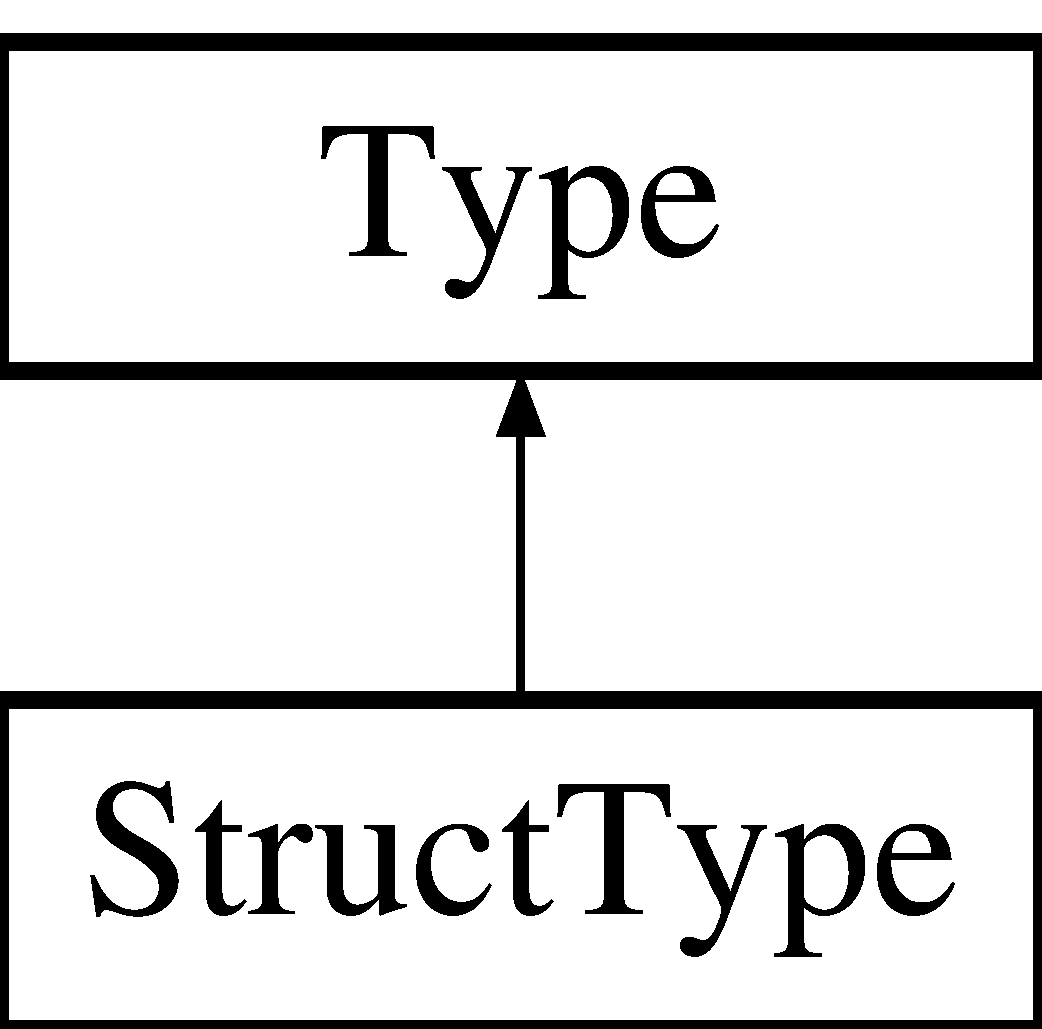
\includegraphics[height=12.000000cm]{classStructType}
\end{center}
\end{figure}
\subsection*{Public Types}
\begin{DoxyCompactItemize}
\item 
enum {\bfseries Derived\-Type} \{ \\*
{\bfseries B\-A\-S\-E}, 
{\bfseries P\-O\-D\-T\-Y\-P\-E}, 
{\bfseries T\-Y\-P\-E\-D\-E\-F\-T\-Y\-P\-E}, 
{\bfseries E\-N\-U\-M\-T\-Y\-P\-E}, 
\\*
{\bfseries A\-R\-R\-A\-Y\-T\-Y\-P\-E}, 
{\bfseries S\-T\-R\-U\-C\-T\-T\-Y\-P\-E}, 
{\bfseries U\-N\-I\-O\-N\-T\-Y\-P\-E}, 
{\bfseries F\-U\-N\-C\-T\-I\-O\-N\-T\-Y\-P\-E}, 
\\*
{\bfseries P\-O\-I\-N\-T\-E\-R\-T\-Y\-P\-E}, 
{\bfseries B\-A\-S\-E}, 
{\bfseries P\-O\-D\-T\-Y\-P\-E}, 
{\bfseries T\-Y\-P\-E\-D\-E\-F\-T\-Y\-P\-E}, 
\\*
{\bfseries E\-N\-U\-M\-T\-Y\-P\-E}, 
{\bfseries A\-R\-R\-A\-Y\-T\-Y\-P\-E}, 
{\bfseries S\-T\-R\-U\-C\-T\-T\-Y\-P\-E}, 
{\bfseries U\-N\-I\-O\-N\-T\-Y\-P\-E}, 
\\*
{\bfseries F\-U\-N\-C\-T\-I\-O\-N\-T\-Y\-P\-E}, 
{\bfseries P\-O\-I\-N\-T\-E\-R\-T\-Y\-P\-E}, 
{\bfseries B\-A\-S\-E}, 
{\bfseries P\-O\-D\-T\-Y\-P\-E}, 
\\*
{\bfseries T\-Y\-P\-E\-D\-E\-F\-T\-Y\-P\-E}, 
{\bfseries E\-N\-U\-M\-T\-Y\-P\-E}, 
{\bfseries A\-R\-R\-A\-Y\-T\-Y\-P\-E}, 
{\bfseries S\-T\-R\-U\-C\-T\-T\-Y\-P\-E}, 
\\*
{\bfseries U\-N\-I\-O\-N\-T\-Y\-P\-E}, 
{\bfseries F\-U\-N\-C\-T\-I\-O\-N\-T\-Y\-P\-E}, 
{\bfseries P\-O\-I\-N\-T\-E\-R\-T\-Y\-P\-E}, 
{\bfseries B\-A\-S\-E}, 
\\*
{\bfseries P\-O\-D\-T\-Y\-P\-E}, 
{\bfseries T\-Y\-P\-E\-D\-E\-F\-T\-Y\-P\-E}, 
{\bfseries E\-N\-U\-M\-T\-Y\-P\-E}, 
{\bfseries A\-R\-R\-A\-Y\-T\-Y\-P\-E}, 
\\*
{\bfseries S\-T\-R\-U\-C\-T\-T\-Y\-P\-E}, 
{\bfseries U\-N\-I\-O\-N\-T\-Y\-P\-E}, 
{\bfseries F\-U\-N\-C\-T\-I\-O\-N\-T\-Y\-P\-E}, 
{\bfseries P\-O\-I\-N\-T\-E\-R\-T\-Y\-P\-E}, 
\\*
{\bfseries B\-A\-S\-E}, 
{\bfseries P\-O\-D\-T\-Y\-P\-E}, 
{\bfseries T\-Y\-P\-E\-D\-E\-F\-T\-Y\-P\-E}, 
{\bfseries E\-N\-U\-M\-T\-Y\-P\-E}, 
\\*
{\bfseries A\-R\-R\-A\-Y\-T\-Y\-P\-E}, 
{\bfseries S\-T\-R\-U\-C\-T\-T\-Y\-P\-E}, 
{\bfseries U\-N\-I\-O\-N\-T\-Y\-P\-E}, 
{\bfseries F\-U\-N\-C\-T\-I\-O\-N\-T\-Y\-P\-E}, 
\\*
{\bfseries P\-O\-I\-N\-T\-E\-R\-T\-Y\-P\-E}, 
{\bfseries B\-A\-S\-E}, 
{\bfseries P\-O\-D\-T\-Y\-P\-E}, 
{\bfseries T\-Y\-P\-E\-D\-E\-F\-T\-Y\-P\-E}, 
\\*
{\bfseries E\-N\-U\-M\-T\-Y\-P\-E}, 
{\bfseries A\-R\-R\-A\-Y\-T\-Y\-P\-E}, 
{\bfseries S\-T\-R\-U\-C\-T\-T\-Y\-P\-E}, 
{\bfseries U\-N\-I\-O\-N\-T\-Y\-P\-E}, 
\\*
{\bfseries F\-U\-N\-C\-T\-I\-O\-N\-T\-Y\-P\-E}, 
{\bfseries P\-O\-I\-N\-T\-E\-R\-T\-Y\-P\-E}, 
{\bfseries B\-A\-S\-E}, 
{\bfseries P\-O\-D\-T\-Y\-P\-E}, 
\\*
{\bfseries T\-Y\-P\-E\-D\-E\-F\-T\-Y\-P\-E}, 
{\bfseries E\-N\-U\-M\-T\-Y\-P\-E}, 
{\bfseries A\-R\-R\-A\-Y\-T\-Y\-P\-E}, 
{\bfseries S\-T\-R\-U\-C\-T\-T\-Y\-P\-E}, 
\\*
{\bfseries U\-N\-I\-O\-N\-T\-Y\-P\-E}, 
{\bfseries F\-U\-N\-C\-T\-I\-O\-N\-T\-Y\-P\-E}, 
{\bfseries P\-O\-I\-N\-T\-E\-R\-T\-Y\-P\-E}, 
{\bfseries B\-A\-S\-E}, 
\\*
{\bfseries P\-O\-D\-T\-Y\-P\-E}, 
{\bfseries T\-Y\-P\-E\-D\-E\-F\-T\-Y\-P\-E}, 
{\bfseries E\-N\-U\-M\-T\-Y\-P\-E}, 
{\bfseries A\-R\-R\-A\-Y\-T\-Y\-P\-E}, 
\\*
{\bfseries S\-T\-R\-U\-C\-T\-T\-Y\-P\-E}, 
{\bfseries U\-N\-I\-O\-N\-T\-Y\-P\-E}, 
{\bfseries F\-U\-N\-C\-T\-I\-O\-N\-T\-Y\-P\-E}, 
{\bfseries P\-O\-I\-N\-T\-E\-R\-T\-Y\-P\-E}, 
\\*
{\bfseries B\-A\-S\-E}, 
{\bfseries P\-O\-D\-T\-Y\-P\-E}, 
{\bfseries T\-Y\-P\-E\-D\-E\-F\-T\-Y\-P\-E}, 
{\bfseries E\-N\-U\-M\-T\-Y\-P\-E}, 
\\*
{\bfseries A\-R\-R\-A\-Y\-T\-Y\-P\-E}, 
{\bfseries S\-T\-R\-U\-C\-T\-T\-Y\-P\-E}, 
{\bfseries U\-N\-I\-O\-N\-T\-Y\-P\-E}, 
{\bfseries F\-U\-N\-C\-T\-I\-O\-N\-T\-Y\-P\-E}, 
\\*
{\bfseries P\-O\-I\-N\-T\-E\-R\-T\-Y\-P\-E}, 
{\bfseries B\-A\-S\-E}, 
{\bfseries P\-O\-D\-T\-Y\-P\-E}, 
{\bfseries T\-Y\-P\-E\-D\-E\-F\-T\-Y\-P\-E}, 
\\*
{\bfseries E\-N\-U\-M\-T\-Y\-P\-E}, 
{\bfseries A\-R\-R\-A\-Y\-T\-Y\-P\-E}, 
{\bfseries S\-T\-R\-U\-C\-T\-T\-Y\-P\-E}, 
{\bfseries U\-N\-I\-O\-N\-T\-Y\-P\-E}, 
\\*
{\bfseries F\-U\-N\-C\-T\-I\-O\-N\-T\-Y\-P\-E}, 
{\bfseries P\-O\-I\-N\-T\-E\-R\-T\-Y\-P\-E}, 
{\bfseries B\-A\-S\-E}, 
{\bfseries P\-O\-D\-T\-Y\-P\-E}, 
\\*
{\bfseries T\-Y\-P\-E\-D\-E\-F\-T\-Y\-P\-E}, 
{\bfseries E\-N\-U\-M\-T\-Y\-P\-E}, 
{\bfseries A\-R\-R\-A\-Y\-T\-Y\-P\-E}, 
{\bfseries S\-T\-R\-U\-C\-T\-T\-Y\-P\-E}, 
\\*
{\bfseries U\-N\-I\-O\-N\-T\-Y\-P\-E}, 
{\bfseries F\-U\-N\-C\-T\-I\-O\-N\-T\-Y\-P\-E}, 
{\bfseries P\-O\-I\-N\-T\-E\-R\-T\-Y\-P\-E}, 
{\bfseries B\-A\-S\-E}, 
\\*
{\bfseries P\-O\-D\-T\-Y\-P\-E}, 
{\bfseries T\-Y\-P\-E\-D\-E\-F\-T\-Y\-P\-E}, 
{\bfseries E\-N\-U\-M\-T\-Y\-P\-E}, 
{\bfseries A\-R\-R\-A\-Y\-T\-Y\-P\-E}, 
\\*
{\bfseries S\-T\-R\-U\-C\-T\-T\-Y\-P\-E}, 
{\bfseries U\-N\-I\-O\-N\-T\-Y\-P\-E}, 
{\bfseries F\-U\-N\-C\-T\-I\-O\-N\-T\-Y\-P\-E}, 
{\bfseries P\-O\-I\-N\-T\-E\-R\-T\-Y\-P\-E}, 
\\*
{\bfseries B\-A\-S\-E}, 
{\bfseries P\-O\-D\-T\-Y\-P\-E}, 
{\bfseries T\-Y\-P\-E\-D\-E\-F\-T\-Y\-P\-E}, 
{\bfseries E\-N\-U\-M\-T\-Y\-P\-E}, 
\\*
{\bfseries A\-R\-R\-A\-Y\-T\-Y\-P\-E}, 
{\bfseries S\-T\-R\-U\-C\-T\-T\-Y\-P\-E}, 
{\bfseries U\-N\-I\-O\-N\-T\-Y\-P\-E}, 
{\bfseries F\-U\-N\-C\-T\-I\-O\-N\-T\-Y\-P\-E}, 
\\*
{\bfseries P\-O\-I\-N\-T\-E\-R\-T\-Y\-P\-E}
 \}
\item 
enum {\bfseries Derived\-Type} \{ \\*
{\bfseries B\-A\-S\-E}, 
{\bfseries P\-O\-D\-T\-Y\-P\-E}, 
{\bfseries T\-Y\-P\-E\-D\-E\-F\-T\-Y\-P\-E}, 
{\bfseries E\-N\-U\-M\-T\-Y\-P\-E}, 
\\*
{\bfseries A\-R\-R\-A\-Y\-T\-Y\-P\-E}, 
{\bfseries S\-T\-R\-U\-C\-T\-T\-Y\-P\-E}, 
{\bfseries U\-N\-I\-O\-N\-T\-Y\-P\-E}, 
{\bfseries F\-U\-N\-C\-T\-I\-O\-N\-T\-Y\-P\-E}, 
\\*
{\bfseries P\-O\-I\-N\-T\-E\-R\-T\-Y\-P\-E}, 
{\bfseries B\-A\-S\-E}, 
{\bfseries P\-O\-D\-T\-Y\-P\-E}, 
{\bfseries T\-Y\-P\-E\-D\-E\-F\-T\-Y\-P\-E}, 
\\*
{\bfseries E\-N\-U\-M\-T\-Y\-P\-E}, 
{\bfseries A\-R\-R\-A\-Y\-T\-Y\-P\-E}, 
{\bfseries S\-T\-R\-U\-C\-T\-T\-Y\-P\-E}, 
{\bfseries U\-N\-I\-O\-N\-T\-Y\-P\-E}, 
\\*
{\bfseries F\-U\-N\-C\-T\-I\-O\-N\-T\-Y\-P\-E}, 
{\bfseries P\-O\-I\-N\-T\-E\-R\-T\-Y\-P\-E}, 
{\bfseries B\-A\-S\-E}, 
{\bfseries P\-O\-D\-T\-Y\-P\-E}, 
\\*
{\bfseries T\-Y\-P\-E\-D\-E\-F\-T\-Y\-P\-E}, 
{\bfseries E\-N\-U\-M\-T\-Y\-P\-E}, 
{\bfseries A\-R\-R\-A\-Y\-T\-Y\-P\-E}, 
{\bfseries S\-T\-R\-U\-C\-T\-T\-Y\-P\-E}, 
\\*
{\bfseries U\-N\-I\-O\-N\-T\-Y\-P\-E}, 
{\bfseries F\-U\-N\-C\-T\-I\-O\-N\-T\-Y\-P\-E}, 
{\bfseries P\-O\-I\-N\-T\-E\-R\-T\-Y\-P\-E}, 
{\bfseries B\-A\-S\-E}, 
\\*
{\bfseries P\-O\-D\-T\-Y\-P\-E}, 
{\bfseries T\-Y\-P\-E\-D\-E\-F\-T\-Y\-P\-E}, 
{\bfseries E\-N\-U\-M\-T\-Y\-P\-E}, 
{\bfseries A\-R\-R\-A\-Y\-T\-Y\-P\-E}, 
\\*
{\bfseries S\-T\-R\-U\-C\-T\-T\-Y\-P\-E}, 
{\bfseries U\-N\-I\-O\-N\-T\-Y\-P\-E}, 
{\bfseries F\-U\-N\-C\-T\-I\-O\-N\-T\-Y\-P\-E}, 
{\bfseries P\-O\-I\-N\-T\-E\-R\-T\-Y\-P\-E}, 
\\*
{\bfseries B\-A\-S\-E}, 
{\bfseries P\-O\-D\-T\-Y\-P\-E}, 
{\bfseries T\-Y\-P\-E\-D\-E\-F\-T\-Y\-P\-E}, 
{\bfseries E\-N\-U\-M\-T\-Y\-P\-E}, 
\\*
{\bfseries A\-R\-R\-A\-Y\-T\-Y\-P\-E}, 
{\bfseries S\-T\-R\-U\-C\-T\-T\-Y\-P\-E}, 
{\bfseries U\-N\-I\-O\-N\-T\-Y\-P\-E}, 
{\bfseries F\-U\-N\-C\-T\-I\-O\-N\-T\-Y\-P\-E}, 
\\*
{\bfseries P\-O\-I\-N\-T\-E\-R\-T\-Y\-P\-E}, 
{\bfseries B\-A\-S\-E}, 
{\bfseries P\-O\-D\-T\-Y\-P\-E}, 
{\bfseries T\-Y\-P\-E\-D\-E\-F\-T\-Y\-P\-E}, 
\\*
{\bfseries E\-N\-U\-M\-T\-Y\-P\-E}, 
{\bfseries A\-R\-R\-A\-Y\-T\-Y\-P\-E}, 
{\bfseries S\-T\-R\-U\-C\-T\-T\-Y\-P\-E}, 
{\bfseries U\-N\-I\-O\-N\-T\-Y\-P\-E}, 
\\*
{\bfseries F\-U\-N\-C\-T\-I\-O\-N\-T\-Y\-P\-E}, 
{\bfseries P\-O\-I\-N\-T\-E\-R\-T\-Y\-P\-E}, 
{\bfseries B\-A\-S\-E}, 
{\bfseries P\-O\-D\-T\-Y\-P\-E}, 
\\*
{\bfseries T\-Y\-P\-E\-D\-E\-F\-T\-Y\-P\-E}, 
{\bfseries E\-N\-U\-M\-T\-Y\-P\-E}, 
{\bfseries A\-R\-R\-A\-Y\-T\-Y\-P\-E}, 
{\bfseries S\-T\-R\-U\-C\-T\-T\-Y\-P\-E}, 
\\*
{\bfseries U\-N\-I\-O\-N\-T\-Y\-P\-E}, 
{\bfseries F\-U\-N\-C\-T\-I\-O\-N\-T\-Y\-P\-E}, 
{\bfseries P\-O\-I\-N\-T\-E\-R\-T\-Y\-P\-E}, 
{\bfseries B\-A\-S\-E}, 
\\*
{\bfseries P\-O\-D\-T\-Y\-P\-E}, 
{\bfseries T\-Y\-P\-E\-D\-E\-F\-T\-Y\-P\-E}, 
{\bfseries E\-N\-U\-M\-T\-Y\-P\-E}, 
{\bfseries A\-R\-R\-A\-Y\-T\-Y\-P\-E}, 
\\*
{\bfseries S\-T\-R\-U\-C\-T\-T\-Y\-P\-E}, 
{\bfseries U\-N\-I\-O\-N\-T\-Y\-P\-E}, 
{\bfseries F\-U\-N\-C\-T\-I\-O\-N\-T\-Y\-P\-E}, 
{\bfseries P\-O\-I\-N\-T\-E\-R\-T\-Y\-P\-E}, 
\\*
{\bfseries B\-A\-S\-E}, 
{\bfseries P\-O\-D\-T\-Y\-P\-E}, 
{\bfseries T\-Y\-P\-E\-D\-E\-F\-T\-Y\-P\-E}, 
{\bfseries E\-N\-U\-M\-T\-Y\-P\-E}, 
\\*
{\bfseries A\-R\-R\-A\-Y\-T\-Y\-P\-E}, 
{\bfseries S\-T\-R\-U\-C\-T\-T\-Y\-P\-E}, 
{\bfseries U\-N\-I\-O\-N\-T\-Y\-P\-E}, 
{\bfseries F\-U\-N\-C\-T\-I\-O\-N\-T\-Y\-P\-E}, 
\\*
{\bfseries P\-O\-I\-N\-T\-E\-R\-T\-Y\-P\-E}, 
{\bfseries B\-A\-S\-E}, 
{\bfseries P\-O\-D\-T\-Y\-P\-E}, 
{\bfseries T\-Y\-P\-E\-D\-E\-F\-T\-Y\-P\-E}, 
\\*
{\bfseries E\-N\-U\-M\-T\-Y\-P\-E}, 
{\bfseries A\-R\-R\-A\-Y\-T\-Y\-P\-E}, 
{\bfseries S\-T\-R\-U\-C\-T\-T\-Y\-P\-E}, 
{\bfseries U\-N\-I\-O\-N\-T\-Y\-P\-E}, 
\\*
{\bfseries F\-U\-N\-C\-T\-I\-O\-N\-T\-Y\-P\-E}, 
{\bfseries P\-O\-I\-N\-T\-E\-R\-T\-Y\-P\-E}, 
{\bfseries B\-A\-S\-E}, 
{\bfseries P\-O\-D\-T\-Y\-P\-E}, 
\\*
{\bfseries T\-Y\-P\-E\-D\-E\-F\-T\-Y\-P\-E}, 
{\bfseries E\-N\-U\-M\-T\-Y\-P\-E}, 
{\bfseries A\-R\-R\-A\-Y\-T\-Y\-P\-E}, 
{\bfseries S\-T\-R\-U\-C\-T\-T\-Y\-P\-E}, 
\\*
{\bfseries U\-N\-I\-O\-N\-T\-Y\-P\-E}, 
{\bfseries F\-U\-N\-C\-T\-I\-O\-N\-T\-Y\-P\-E}, 
{\bfseries P\-O\-I\-N\-T\-E\-R\-T\-Y\-P\-E}, 
{\bfseries B\-A\-S\-E}, 
\\*
{\bfseries P\-O\-D\-T\-Y\-P\-E}, 
{\bfseries T\-Y\-P\-E\-D\-E\-F\-T\-Y\-P\-E}, 
{\bfseries E\-N\-U\-M\-T\-Y\-P\-E}, 
{\bfseries A\-R\-R\-A\-Y\-T\-Y\-P\-E}, 
\\*
{\bfseries S\-T\-R\-U\-C\-T\-T\-Y\-P\-E}, 
{\bfseries U\-N\-I\-O\-N\-T\-Y\-P\-E}, 
{\bfseries F\-U\-N\-C\-T\-I\-O\-N\-T\-Y\-P\-E}, 
{\bfseries P\-O\-I\-N\-T\-E\-R\-T\-Y\-P\-E}, 
\\*
{\bfseries B\-A\-S\-E}, 
{\bfseries P\-O\-D\-T\-Y\-P\-E}, 
{\bfseries T\-Y\-P\-E\-D\-E\-F\-T\-Y\-P\-E}, 
{\bfseries E\-N\-U\-M\-T\-Y\-P\-E}, 
\\*
{\bfseries A\-R\-R\-A\-Y\-T\-Y\-P\-E}, 
{\bfseries S\-T\-R\-U\-C\-T\-T\-Y\-P\-E}, 
{\bfseries U\-N\-I\-O\-N\-T\-Y\-P\-E}, 
{\bfseries F\-U\-N\-C\-T\-I\-O\-N\-T\-Y\-P\-E}, 
\\*
{\bfseries P\-O\-I\-N\-T\-E\-R\-T\-Y\-P\-E}
 \}
\item 
enum {\bfseries Derived\-Type} \{ \\*
{\bfseries B\-A\-S\-E}, 
{\bfseries P\-O\-D\-T\-Y\-P\-E}, 
{\bfseries T\-Y\-P\-E\-D\-E\-F\-T\-Y\-P\-E}, 
{\bfseries E\-N\-U\-M\-T\-Y\-P\-E}, 
\\*
{\bfseries A\-R\-R\-A\-Y\-T\-Y\-P\-E}, 
{\bfseries S\-T\-R\-U\-C\-T\-T\-Y\-P\-E}, 
{\bfseries U\-N\-I\-O\-N\-T\-Y\-P\-E}, 
{\bfseries F\-U\-N\-C\-T\-I\-O\-N\-T\-Y\-P\-E}, 
\\*
{\bfseries P\-O\-I\-N\-T\-E\-R\-T\-Y\-P\-E}, 
{\bfseries B\-A\-S\-E}, 
{\bfseries P\-O\-D\-T\-Y\-P\-E}, 
{\bfseries T\-Y\-P\-E\-D\-E\-F\-T\-Y\-P\-E}, 
\\*
{\bfseries E\-N\-U\-M\-T\-Y\-P\-E}, 
{\bfseries A\-R\-R\-A\-Y\-T\-Y\-P\-E}, 
{\bfseries S\-T\-R\-U\-C\-T\-T\-Y\-P\-E}, 
{\bfseries U\-N\-I\-O\-N\-T\-Y\-P\-E}, 
\\*
{\bfseries F\-U\-N\-C\-T\-I\-O\-N\-T\-Y\-P\-E}, 
{\bfseries P\-O\-I\-N\-T\-E\-R\-T\-Y\-P\-E}, 
{\bfseries B\-A\-S\-E}, 
{\bfseries P\-O\-D\-T\-Y\-P\-E}, 
\\*
{\bfseries T\-Y\-P\-E\-D\-E\-F\-T\-Y\-P\-E}, 
{\bfseries E\-N\-U\-M\-T\-Y\-P\-E}, 
{\bfseries A\-R\-R\-A\-Y\-T\-Y\-P\-E}, 
{\bfseries S\-T\-R\-U\-C\-T\-T\-Y\-P\-E}, 
\\*
{\bfseries U\-N\-I\-O\-N\-T\-Y\-P\-E}, 
{\bfseries F\-U\-N\-C\-T\-I\-O\-N\-T\-Y\-P\-E}, 
{\bfseries P\-O\-I\-N\-T\-E\-R\-T\-Y\-P\-E}, 
{\bfseries B\-A\-S\-E}, 
\\*
{\bfseries P\-O\-D\-T\-Y\-P\-E}, 
{\bfseries T\-Y\-P\-E\-D\-E\-F\-T\-Y\-P\-E}, 
{\bfseries E\-N\-U\-M\-T\-Y\-P\-E}, 
{\bfseries A\-R\-R\-A\-Y\-T\-Y\-P\-E}, 
\\*
{\bfseries S\-T\-R\-U\-C\-T\-T\-Y\-P\-E}, 
{\bfseries U\-N\-I\-O\-N\-T\-Y\-P\-E}, 
{\bfseries F\-U\-N\-C\-T\-I\-O\-N\-T\-Y\-P\-E}, 
{\bfseries P\-O\-I\-N\-T\-E\-R\-T\-Y\-P\-E}, 
\\*
{\bfseries B\-A\-S\-E}, 
{\bfseries P\-O\-D\-T\-Y\-P\-E}, 
{\bfseries T\-Y\-P\-E\-D\-E\-F\-T\-Y\-P\-E}, 
{\bfseries E\-N\-U\-M\-T\-Y\-P\-E}, 
\\*
{\bfseries A\-R\-R\-A\-Y\-T\-Y\-P\-E}, 
{\bfseries S\-T\-R\-U\-C\-T\-T\-Y\-P\-E}, 
{\bfseries U\-N\-I\-O\-N\-T\-Y\-P\-E}, 
{\bfseries F\-U\-N\-C\-T\-I\-O\-N\-T\-Y\-P\-E}, 
\\*
{\bfseries P\-O\-I\-N\-T\-E\-R\-T\-Y\-P\-E}, 
{\bfseries B\-A\-S\-E}, 
{\bfseries P\-O\-D\-T\-Y\-P\-E}, 
{\bfseries T\-Y\-P\-E\-D\-E\-F\-T\-Y\-P\-E}, 
\\*
{\bfseries E\-N\-U\-M\-T\-Y\-P\-E}, 
{\bfseries A\-R\-R\-A\-Y\-T\-Y\-P\-E}, 
{\bfseries S\-T\-R\-U\-C\-T\-T\-Y\-P\-E}, 
{\bfseries U\-N\-I\-O\-N\-T\-Y\-P\-E}, 
\\*
{\bfseries F\-U\-N\-C\-T\-I\-O\-N\-T\-Y\-P\-E}, 
{\bfseries P\-O\-I\-N\-T\-E\-R\-T\-Y\-P\-E}, 
{\bfseries B\-A\-S\-E}, 
{\bfseries P\-O\-D\-T\-Y\-P\-E}, 
\\*
{\bfseries T\-Y\-P\-E\-D\-E\-F\-T\-Y\-P\-E}, 
{\bfseries E\-N\-U\-M\-T\-Y\-P\-E}, 
{\bfseries A\-R\-R\-A\-Y\-T\-Y\-P\-E}, 
{\bfseries S\-T\-R\-U\-C\-T\-T\-Y\-P\-E}, 
\\*
{\bfseries U\-N\-I\-O\-N\-T\-Y\-P\-E}, 
{\bfseries F\-U\-N\-C\-T\-I\-O\-N\-T\-Y\-P\-E}, 
{\bfseries P\-O\-I\-N\-T\-E\-R\-T\-Y\-P\-E}, 
{\bfseries B\-A\-S\-E}, 
\\*
{\bfseries P\-O\-D\-T\-Y\-P\-E}, 
{\bfseries T\-Y\-P\-E\-D\-E\-F\-T\-Y\-P\-E}, 
{\bfseries E\-N\-U\-M\-T\-Y\-P\-E}, 
{\bfseries A\-R\-R\-A\-Y\-T\-Y\-P\-E}, 
\\*
{\bfseries S\-T\-R\-U\-C\-T\-T\-Y\-P\-E}, 
{\bfseries U\-N\-I\-O\-N\-T\-Y\-P\-E}, 
{\bfseries F\-U\-N\-C\-T\-I\-O\-N\-T\-Y\-P\-E}, 
{\bfseries P\-O\-I\-N\-T\-E\-R\-T\-Y\-P\-E}, 
\\*
{\bfseries B\-A\-S\-E}, 
{\bfseries P\-O\-D\-T\-Y\-P\-E}, 
{\bfseries T\-Y\-P\-E\-D\-E\-F\-T\-Y\-P\-E}, 
{\bfseries E\-N\-U\-M\-T\-Y\-P\-E}, 
\\*
{\bfseries A\-R\-R\-A\-Y\-T\-Y\-P\-E}, 
{\bfseries S\-T\-R\-U\-C\-T\-T\-Y\-P\-E}, 
{\bfseries U\-N\-I\-O\-N\-T\-Y\-P\-E}, 
{\bfseries F\-U\-N\-C\-T\-I\-O\-N\-T\-Y\-P\-E}, 
\\*
{\bfseries P\-O\-I\-N\-T\-E\-R\-T\-Y\-P\-E}, 
{\bfseries B\-A\-S\-E}, 
{\bfseries P\-O\-D\-T\-Y\-P\-E}, 
{\bfseries T\-Y\-P\-E\-D\-E\-F\-T\-Y\-P\-E}, 
\\*
{\bfseries E\-N\-U\-M\-T\-Y\-P\-E}, 
{\bfseries A\-R\-R\-A\-Y\-T\-Y\-P\-E}, 
{\bfseries S\-T\-R\-U\-C\-T\-T\-Y\-P\-E}, 
{\bfseries U\-N\-I\-O\-N\-T\-Y\-P\-E}, 
\\*
{\bfseries F\-U\-N\-C\-T\-I\-O\-N\-T\-Y\-P\-E}, 
{\bfseries P\-O\-I\-N\-T\-E\-R\-T\-Y\-P\-E}, 
{\bfseries B\-A\-S\-E}, 
{\bfseries P\-O\-D\-T\-Y\-P\-E}, 
\\*
{\bfseries T\-Y\-P\-E\-D\-E\-F\-T\-Y\-P\-E}, 
{\bfseries E\-N\-U\-M\-T\-Y\-P\-E}, 
{\bfseries A\-R\-R\-A\-Y\-T\-Y\-P\-E}, 
{\bfseries S\-T\-R\-U\-C\-T\-T\-Y\-P\-E}, 
\\*
{\bfseries U\-N\-I\-O\-N\-T\-Y\-P\-E}, 
{\bfseries F\-U\-N\-C\-T\-I\-O\-N\-T\-Y\-P\-E}, 
{\bfseries P\-O\-I\-N\-T\-E\-R\-T\-Y\-P\-E}, 
{\bfseries B\-A\-S\-E}, 
\\*
{\bfseries P\-O\-D\-T\-Y\-P\-E}, 
{\bfseries T\-Y\-P\-E\-D\-E\-F\-T\-Y\-P\-E}, 
{\bfseries E\-N\-U\-M\-T\-Y\-P\-E}, 
{\bfseries A\-R\-R\-A\-Y\-T\-Y\-P\-E}, 
\\*
{\bfseries S\-T\-R\-U\-C\-T\-T\-Y\-P\-E}, 
{\bfseries U\-N\-I\-O\-N\-T\-Y\-P\-E}, 
{\bfseries F\-U\-N\-C\-T\-I\-O\-N\-T\-Y\-P\-E}, 
{\bfseries P\-O\-I\-N\-T\-E\-R\-T\-Y\-P\-E}, 
\\*
{\bfseries B\-A\-S\-E}, 
{\bfseries P\-O\-D\-T\-Y\-P\-E}, 
{\bfseries T\-Y\-P\-E\-D\-E\-F\-T\-Y\-P\-E}, 
{\bfseries E\-N\-U\-M\-T\-Y\-P\-E}, 
\\*
{\bfseries A\-R\-R\-A\-Y\-T\-Y\-P\-E}, 
{\bfseries S\-T\-R\-U\-C\-T\-T\-Y\-P\-E}, 
{\bfseries U\-N\-I\-O\-N\-T\-Y\-P\-E}, 
{\bfseries F\-U\-N\-C\-T\-I\-O\-N\-T\-Y\-P\-E}, 
\\*
{\bfseries P\-O\-I\-N\-T\-E\-R\-T\-Y\-P\-E}
 \}
\item 
enum {\bfseries Derived\-Type} \{ \\*
{\bfseries B\-A\-S\-E}, 
{\bfseries P\-O\-D\-T\-Y\-P\-E}, 
{\bfseries T\-Y\-P\-E\-D\-E\-F\-T\-Y\-P\-E}, 
{\bfseries E\-N\-U\-M\-T\-Y\-P\-E}, 
\\*
{\bfseries A\-R\-R\-A\-Y\-T\-Y\-P\-E}, 
{\bfseries S\-T\-R\-U\-C\-T\-T\-Y\-P\-E}, 
{\bfseries U\-N\-I\-O\-N\-T\-Y\-P\-E}, 
{\bfseries F\-U\-N\-C\-T\-I\-O\-N\-T\-Y\-P\-E}, 
\\*
{\bfseries P\-O\-I\-N\-T\-E\-R\-T\-Y\-P\-E}, 
{\bfseries B\-A\-S\-E}, 
{\bfseries P\-O\-D\-T\-Y\-P\-E}, 
{\bfseries T\-Y\-P\-E\-D\-E\-F\-T\-Y\-P\-E}, 
\\*
{\bfseries E\-N\-U\-M\-T\-Y\-P\-E}, 
{\bfseries A\-R\-R\-A\-Y\-T\-Y\-P\-E}, 
{\bfseries S\-T\-R\-U\-C\-T\-T\-Y\-P\-E}, 
{\bfseries U\-N\-I\-O\-N\-T\-Y\-P\-E}, 
\\*
{\bfseries F\-U\-N\-C\-T\-I\-O\-N\-T\-Y\-P\-E}, 
{\bfseries P\-O\-I\-N\-T\-E\-R\-T\-Y\-P\-E}, 
{\bfseries B\-A\-S\-E}, 
{\bfseries P\-O\-D\-T\-Y\-P\-E}, 
\\*
{\bfseries T\-Y\-P\-E\-D\-E\-F\-T\-Y\-P\-E}, 
{\bfseries E\-N\-U\-M\-T\-Y\-P\-E}, 
{\bfseries A\-R\-R\-A\-Y\-T\-Y\-P\-E}, 
{\bfseries S\-T\-R\-U\-C\-T\-T\-Y\-P\-E}, 
\\*
{\bfseries U\-N\-I\-O\-N\-T\-Y\-P\-E}, 
{\bfseries F\-U\-N\-C\-T\-I\-O\-N\-T\-Y\-P\-E}, 
{\bfseries P\-O\-I\-N\-T\-E\-R\-T\-Y\-P\-E}, 
{\bfseries B\-A\-S\-E}, 
\\*
{\bfseries P\-O\-D\-T\-Y\-P\-E}, 
{\bfseries T\-Y\-P\-E\-D\-E\-F\-T\-Y\-P\-E}, 
{\bfseries E\-N\-U\-M\-T\-Y\-P\-E}, 
{\bfseries A\-R\-R\-A\-Y\-T\-Y\-P\-E}, 
\\*
{\bfseries S\-T\-R\-U\-C\-T\-T\-Y\-P\-E}, 
{\bfseries U\-N\-I\-O\-N\-T\-Y\-P\-E}, 
{\bfseries F\-U\-N\-C\-T\-I\-O\-N\-T\-Y\-P\-E}, 
{\bfseries P\-O\-I\-N\-T\-E\-R\-T\-Y\-P\-E}, 
\\*
{\bfseries B\-A\-S\-E}, 
{\bfseries P\-O\-D\-T\-Y\-P\-E}, 
{\bfseries T\-Y\-P\-E\-D\-E\-F\-T\-Y\-P\-E}, 
{\bfseries E\-N\-U\-M\-T\-Y\-P\-E}, 
\\*
{\bfseries A\-R\-R\-A\-Y\-T\-Y\-P\-E}, 
{\bfseries S\-T\-R\-U\-C\-T\-T\-Y\-P\-E}, 
{\bfseries U\-N\-I\-O\-N\-T\-Y\-P\-E}, 
{\bfseries F\-U\-N\-C\-T\-I\-O\-N\-T\-Y\-P\-E}, 
\\*
{\bfseries P\-O\-I\-N\-T\-E\-R\-T\-Y\-P\-E}, 
{\bfseries B\-A\-S\-E}, 
{\bfseries P\-O\-D\-T\-Y\-P\-E}, 
{\bfseries T\-Y\-P\-E\-D\-E\-F\-T\-Y\-P\-E}, 
\\*
{\bfseries E\-N\-U\-M\-T\-Y\-P\-E}, 
{\bfseries A\-R\-R\-A\-Y\-T\-Y\-P\-E}, 
{\bfseries S\-T\-R\-U\-C\-T\-T\-Y\-P\-E}, 
{\bfseries U\-N\-I\-O\-N\-T\-Y\-P\-E}, 
\\*
{\bfseries F\-U\-N\-C\-T\-I\-O\-N\-T\-Y\-P\-E}, 
{\bfseries P\-O\-I\-N\-T\-E\-R\-T\-Y\-P\-E}, 
{\bfseries B\-A\-S\-E}, 
{\bfseries P\-O\-D\-T\-Y\-P\-E}, 
\\*
{\bfseries T\-Y\-P\-E\-D\-E\-F\-T\-Y\-P\-E}, 
{\bfseries E\-N\-U\-M\-T\-Y\-P\-E}, 
{\bfseries A\-R\-R\-A\-Y\-T\-Y\-P\-E}, 
{\bfseries S\-T\-R\-U\-C\-T\-T\-Y\-P\-E}, 
\\*
{\bfseries U\-N\-I\-O\-N\-T\-Y\-P\-E}, 
{\bfseries F\-U\-N\-C\-T\-I\-O\-N\-T\-Y\-P\-E}, 
{\bfseries P\-O\-I\-N\-T\-E\-R\-T\-Y\-P\-E}, 
{\bfseries B\-A\-S\-E}, 
\\*
{\bfseries P\-O\-D\-T\-Y\-P\-E}, 
{\bfseries T\-Y\-P\-E\-D\-E\-F\-T\-Y\-P\-E}, 
{\bfseries E\-N\-U\-M\-T\-Y\-P\-E}, 
{\bfseries A\-R\-R\-A\-Y\-T\-Y\-P\-E}, 
\\*
{\bfseries S\-T\-R\-U\-C\-T\-T\-Y\-P\-E}, 
{\bfseries U\-N\-I\-O\-N\-T\-Y\-P\-E}, 
{\bfseries F\-U\-N\-C\-T\-I\-O\-N\-T\-Y\-P\-E}, 
{\bfseries P\-O\-I\-N\-T\-E\-R\-T\-Y\-P\-E}, 
\\*
{\bfseries B\-A\-S\-E}, 
{\bfseries P\-O\-D\-T\-Y\-P\-E}, 
{\bfseries T\-Y\-P\-E\-D\-E\-F\-T\-Y\-P\-E}, 
{\bfseries E\-N\-U\-M\-T\-Y\-P\-E}, 
\\*
{\bfseries A\-R\-R\-A\-Y\-T\-Y\-P\-E}, 
{\bfseries S\-T\-R\-U\-C\-T\-T\-Y\-P\-E}, 
{\bfseries U\-N\-I\-O\-N\-T\-Y\-P\-E}, 
{\bfseries F\-U\-N\-C\-T\-I\-O\-N\-T\-Y\-P\-E}, 
\\*
{\bfseries P\-O\-I\-N\-T\-E\-R\-T\-Y\-P\-E}, 
{\bfseries B\-A\-S\-E}, 
{\bfseries P\-O\-D\-T\-Y\-P\-E}, 
{\bfseries T\-Y\-P\-E\-D\-E\-F\-T\-Y\-P\-E}, 
\\*
{\bfseries E\-N\-U\-M\-T\-Y\-P\-E}, 
{\bfseries A\-R\-R\-A\-Y\-T\-Y\-P\-E}, 
{\bfseries S\-T\-R\-U\-C\-T\-T\-Y\-P\-E}, 
{\bfseries U\-N\-I\-O\-N\-T\-Y\-P\-E}, 
\\*
{\bfseries F\-U\-N\-C\-T\-I\-O\-N\-T\-Y\-P\-E}, 
{\bfseries P\-O\-I\-N\-T\-E\-R\-T\-Y\-P\-E}, 
{\bfseries B\-A\-S\-E}, 
{\bfseries P\-O\-D\-T\-Y\-P\-E}, 
\\*
{\bfseries T\-Y\-P\-E\-D\-E\-F\-T\-Y\-P\-E}, 
{\bfseries E\-N\-U\-M\-T\-Y\-P\-E}, 
{\bfseries A\-R\-R\-A\-Y\-T\-Y\-P\-E}, 
{\bfseries S\-T\-R\-U\-C\-T\-T\-Y\-P\-E}, 
\\*
{\bfseries U\-N\-I\-O\-N\-T\-Y\-P\-E}, 
{\bfseries F\-U\-N\-C\-T\-I\-O\-N\-T\-Y\-P\-E}, 
{\bfseries P\-O\-I\-N\-T\-E\-R\-T\-Y\-P\-E}, 
{\bfseries B\-A\-S\-E}, 
\\*
{\bfseries P\-O\-D\-T\-Y\-P\-E}, 
{\bfseries T\-Y\-P\-E\-D\-E\-F\-T\-Y\-P\-E}, 
{\bfseries E\-N\-U\-M\-T\-Y\-P\-E}, 
{\bfseries A\-R\-R\-A\-Y\-T\-Y\-P\-E}, 
\\*
{\bfseries S\-T\-R\-U\-C\-T\-T\-Y\-P\-E}, 
{\bfseries U\-N\-I\-O\-N\-T\-Y\-P\-E}, 
{\bfseries F\-U\-N\-C\-T\-I\-O\-N\-T\-Y\-P\-E}, 
{\bfseries P\-O\-I\-N\-T\-E\-R\-T\-Y\-P\-E}, 
\\*
{\bfseries B\-A\-S\-E}, 
{\bfseries P\-O\-D\-T\-Y\-P\-E}, 
{\bfseries T\-Y\-P\-E\-D\-E\-F\-T\-Y\-P\-E}, 
{\bfseries E\-N\-U\-M\-T\-Y\-P\-E}, 
\\*
{\bfseries A\-R\-R\-A\-Y\-T\-Y\-P\-E}, 
{\bfseries S\-T\-R\-U\-C\-T\-T\-Y\-P\-E}, 
{\bfseries U\-N\-I\-O\-N\-T\-Y\-P\-E}, 
{\bfseries F\-U\-N\-C\-T\-I\-O\-N\-T\-Y\-P\-E}, 
\\*
{\bfseries P\-O\-I\-N\-T\-E\-R\-T\-Y\-P\-E}
 \}
\item 
enum {\bfseries Derived\-Type} \{ \\*
{\bfseries B\-A\-S\-E}, 
{\bfseries P\-O\-D\-T\-Y\-P\-E}, 
{\bfseries T\-Y\-P\-E\-D\-E\-F\-T\-Y\-P\-E}, 
{\bfseries E\-N\-U\-M\-T\-Y\-P\-E}, 
\\*
{\bfseries A\-R\-R\-A\-Y\-T\-Y\-P\-E}, 
{\bfseries S\-T\-R\-U\-C\-T\-T\-Y\-P\-E}, 
{\bfseries U\-N\-I\-O\-N\-T\-Y\-P\-E}, 
{\bfseries F\-U\-N\-C\-T\-I\-O\-N\-T\-Y\-P\-E}, 
\\*
{\bfseries P\-O\-I\-N\-T\-E\-R\-T\-Y\-P\-E}, 
{\bfseries B\-A\-S\-E}, 
{\bfseries P\-O\-D\-T\-Y\-P\-E}, 
{\bfseries T\-Y\-P\-E\-D\-E\-F\-T\-Y\-P\-E}, 
\\*
{\bfseries E\-N\-U\-M\-T\-Y\-P\-E}, 
{\bfseries A\-R\-R\-A\-Y\-T\-Y\-P\-E}, 
{\bfseries S\-T\-R\-U\-C\-T\-T\-Y\-P\-E}, 
{\bfseries U\-N\-I\-O\-N\-T\-Y\-P\-E}, 
\\*
{\bfseries F\-U\-N\-C\-T\-I\-O\-N\-T\-Y\-P\-E}, 
{\bfseries P\-O\-I\-N\-T\-E\-R\-T\-Y\-P\-E}, 
{\bfseries B\-A\-S\-E}, 
{\bfseries P\-O\-D\-T\-Y\-P\-E}, 
\\*
{\bfseries T\-Y\-P\-E\-D\-E\-F\-T\-Y\-P\-E}, 
{\bfseries E\-N\-U\-M\-T\-Y\-P\-E}, 
{\bfseries A\-R\-R\-A\-Y\-T\-Y\-P\-E}, 
{\bfseries S\-T\-R\-U\-C\-T\-T\-Y\-P\-E}, 
\\*
{\bfseries U\-N\-I\-O\-N\-T\-Y\-P\-E}, 
{\bfseries F\-U\-N\-C\-T\-I\-O\-N\-T\-Y\-P\-E}, 
{\bfseries P\-O\-I\-N\-T\-E\-R\-T\-Y\-P\-E}, 
{\bfseries B\-A\-S\-E}, 
\\*
{\bfseries P\-O\-D\-T\-Y\-P\-E}, 
{\bfseries T\-Y\-P\-E\-D\-E\-F\-T\-Y\-P\-E}, 
{\bfseries E\-N\-U\-M\-T\-Y\-P\-E}, 
{\bfseries A\-R\-R\-A\-Y\-T\-Y\-P\-E}, 
\\*
{\bfseries S\-T\-R\-U\-C\-T\-T\-Y\-P\-E}, 
{\bfseries U\-N\-I\-O\-N\-T\-Y\-P\-E}, 
{\bfseries F\-U\-N\-C\-T\-I\-O\-N\-T\-Y\-P\-E}, 
{\bfseries P\-O\-I\-N\-T\-E\-R\-T\-Y\-P\-E}, 
\\*
{\bfseries B\-A\-S\-E}, 
{\bfseries P\-O\-D\-T\-Y\-P\-E}, 
{\bfseries T\-Y\-P\-E\-D\-E\-F\-T\-Y\-P\-E}, 
{\bfseries E\-N\-U\-M\-T\-Y\-P\-E}, 
\\*
{\bfseries A\-R\-R\-A\-Y\-T\-Y\-P\-E}, 
{\bfseries S\-T\-R\-U\-C\-T\-T\-Y\-P\-E}, 
{\bfseries U\-N\-I\-O\-N\-T\-Y\-P\-E}, 
{\bfseries F\-U\-N\-C\-T\-I\-O\-N\-T\-Y\-P\-E}, 
\\*
{\bfseries P\-O\-I\-N\-T\-E\-R\-T\-Y\-P\-E}, 
{\bfseries B\-A\-S\-E}, 
{\bfseries P\-O\-D\-T\-Y\-P\-E}, 
{\bfseries T\-Y\-P\-E\-D\-E\-F\-T\-Y\-P\-E}, 
\\*
{\bfseries E\-N\-U\-M\-T\-Y\-P\-E}, 
{\bfseries A\-R\-R\-A\-Y\-T\-Y\-P\-E}, 
{\bfseries S\-T\-R\-U\-C\-T\-T\-Y\-P\-E}, 
{\bfseries U\-N\-I\-O\-N\-T\-Y\-P\-E}, 
\\*
{\bfseries F\-U\-N\-C\-T\-I\-O\-N\-T\-Y\-P\-E}, 
{\bfseries P\-O\-I\-N\-T\-E\-R\-T\-Y\-P\-E}, 
{\bfseries B\-A\-S\-E}, 
{\bfseries P\-O\-D\-T\-Y\-P\-E}, 
\\*
{\bfseries T\-Y\-P\-E\-D\-E\-F\-T\-Y\-P\-E}, 
{\bfseries E\-N\-U\-M\-T\-Y\-P\-E}, 
{\bfseries A\-R\-R\-A\-Y\-T\-Y\-P\-E}, 
{\bfseries S\-T\-R\-U\-C\-T\-T\-Y\-P\-E}, 
\\*
{\bfseries U\-N\-I\-O\-N\-T\-Y\-P\-E}, 
{\bfseries F\-U\-N\-C\-T\-I\-O\-N\-T\-Y\-P\-E}, 
{\bfseries P\-O\-I\-N\-T\-E\-R\-T\-Y\-P\-E}, 
{\bfseries B\-A\-S\-E}, 
\\*
{\bfseries P\-O\-D\-T\-Y\-P\-E}, 
{\bfseries T\-Y\-P\-E\-D\-E\-F\-T\-Y\-P\-E}, 
{\bfseries E\-N\-U\-M\-T\-Y\-P\-E}, 
{\bfseries A\-R\-R\-A\-Y\-T\-Y\-P\-E}, 
\\*
{\bfseries S\-T\-R\-U\-C\-T\-T\-Y\-P\-E}, 
{\bfseries U\-N\-I\-O\-N\-T\-Y\-P\-E}, 
{\bfseries F\-U\-N\-C\-T\-I\-O\-N\-T\-Y\-P\-E}, 
{\bfseries P\-O\-I\-N\-T\-E\-R\-T\-Y\-P\-E}, 
\\*
{\bfseries B\-A\-S\-E}, 
{\bfseries P\-O\-D\-T\-Y\-P\-E}, 
{\bfseries T\-Y\-P\-E\-D\-E\-F\-T\-Y\-P\-E}, 
{\bfseries E\-N\-U\-M\-T\-Y\-P\-E}, 
\\*
{\bfseries A\-R\-R\-A\-Y\-T\-Y\-P\-E}, 
{\bfseries S\-T\-R\-U\-C\-T\-T\-Y\-P\-E}, 
{\bfseries U\-N\-I\-O\-N\-T\-Y\-P\-E}, 
{\bfseries F\-U\-N\-C\-T\-I\-O\-N\-T\-Y\-P\-E}, 
\\*
{\bfseries P\-O\-I\-N\-T\-E\-R\-T\-Y\-P\-E}, 
{\bfseries B\-A\-S\-E}, 
{\bfseries P\-O\-D\-T\-Y\-P\-E}, 
{\bfseries T\-Y\-P\-E\-D\-E\-F\-T\-Y\-P\-E}, 
\\*
{\bfseries E\-N\-U\-M\-T\-Y\-P\-E}, 
{\bfseries A\-R\-R\-A\-Y\-T\-Y\-P\-E}, 
{\bfseries S\-T\-R\-U\-C\-T\-T\-Y\-P\-E}, 
{\bfseries U\-N\-I\-O\-N\-T\-Y\-P\-E}, 
\\*
{\bfseries F\-U\-N\-C\-T\-I\-O\-N\-T\-Y\-P\-E}, 
{\bfseries P\-O\-I\-N\-T\-E\-R\-T\-Y\-P\-E}, 
{\bfseries B\-A\-S\-E}, 
{\bfseries P\-O\-D\-T\-Y\-P\-E}, 
\\*
{\bfseries T\-Y\-P\-E\-D\-E\-F\-T\-Y\-P\-E}, 
{\bfseries E\-N\-U\-M\-T\-Y\-P\-E}, 
{\bfseries A\-R\-R\-A\-Y\-T\-Y\-P\-E}, 
{\bfseries S\-T\-R\-U\-C\-T\-T\-Y\-P\-E}, 
\\*
{\bfseries U\-N\-I\-O\-N\-T\-Y\-P\-E}, 
{\bfseries F\-U\-N\-C\-T\-I\-O\-N\-T\-Y\-P\-E}, 
{\bfseries P\-O\-I\-N\-T\-E\-R\-T\-Y\-P\-E}, 
{\bfseries B\-A\-S\-E}, 
\\*
{\bfseries P\-O\-D\-T\-Y\-P\-E}, 
{\bfseries T\-Y\-P\-E\-D\-E\-F\-T\-Y\-P\-E}, 
{\bfseries E\-N\-U\-M\-T\-Y\-P\-E}, 
{\bfseries A\-R\-R\-A\-Y\-T\-Y\-P\-E}, 
\\*
{\bfseries S\-T\-R\-U\-C\-T\-T\-Y\-P\-E}, 
{\bfseries U\-N\-I\-O\-N\-T\-Y\-P\-E}, 
{\bfseries F\-U\-N\-C\-T\-I\-O\-N\-T\-Y\-P\-E}, 
{\bfseries P\-O\-I\-N\-T\-E\-R\-T\-Y\-P\-E}, 
\\*
{\bfseries B\-A\-S\-E}, 
{\bfseries P\-O\-D\-T\-Y\-P\-E}, 
{\bfseries T\-Y\-P\-E\-D\-E\-F\-T\-Y\-P\-E}, 
{\bfseries E\-N\-U\-M\-T\-Y\-P\-E}, 
\\*
{\bfseries A\-R\-R\-A\-Y\-T\-Y\-P\-E}, 
{\bfseries S\-T\-R\-U\-C\-T\-T\-Y\-P\-E}, 
{\bfseries U\-N\-I\-O\-N\-T\-Y\-P\-E}, 
{\bfseries F\-U\-N\-C\-T\-I\-O\-N\-T\-Y\-P\-E}, 
\\*
{\bfseries P\-O\-I\-N\-T\-E\-R\-T\-Y\-P\-E}
 \}
\item 
enum {\bfseries Derived\-Type} \{ \\*
{\bfseries B\-A\-S\-E}, 
{\bfseries P\-O\-D\-T\-Y\-P\-E}, 
{\bfseries T\-Y\-P\-E\-D\-E\-F\-T\-Y\-P\-E}, 
{\bfseries E\-N\-U\-M\-T\-Y\-P\-E}, 
\\*
{\bfseries A\-R\-R\-A\-Y\-T\-Y\-P\-E}, 
{\bfseries S\-T\-R\-U\-C\-T\-T\-Y\-P\-E}, 
{\bfseries U\-N\-I\-O\-N\-T\-Y\-P\-E}, 
{\bfseries F\-U\-N\-C\-T\-I\-O\-N\-T\-Y\-P\-E}, 
\\*
{\bfseries P\-O\-I\-N\-T\-E\-R\-T\-Y\-P\-E}, 
{\bfseries B\-A\-S\-E}, 
{\bfseries P\-O\-D\-T\-Y\-P\-E}, 
{\bfseries T\-Y\-P\-E\-D\-E\-F\-T\-Y\-P\-E}, 
\\*
{\bfseries E\-N\-U\-M\-T\-Y\-P\-E}, 
{\bfseries A\-R\-R\-A\-Y\-T\-Y\-P\-E}, 
{\bfseries S\-T\-R\-U\-C\-T\-T\-Y\-P\-E}, 
{\bfseries U\-N\-I\-O\-N\-T\-Y\-P\-E}, 
\\*
{\bfseries F\-U\-N\-C\-T\-I\-O\-N\-T\-Y\-P\-E}, 
{\bfseries P\-O\-I\-N\-T\-E\-R\-T\-Y\-P\-E}, 
{\bfseries B\-A\-S\-E}, 
{\bfseries P\-O\-D\-T\-Y\-P\-E}, 
\\*
{\bfseries T\-Y\-P\-E\-D\-E\-F\-T\-Y\-P\-E}, 
{\bfseries E\-N\-U\-M\-T\-Y\-P\-E}, 
{\bfseries A\-R\-R\-A\-Y\-T\-Y\-P\-E}, 
{\bfseries S\-T\-R\-U\-C\-T\-T\-Y\-P\-E}, 
\\*
{\bfseries U\-N\-I\-O\-N\-T\-Y\-P\-E}, 
{\bfseries F\-U\-N\-C\-T\-I\-O\-N\-T\-Y\-P\-E}, 
{\bfseries P\-O\-I\-N\-T\-E\-R\-T\-Y\-P\-E}, 
{\bfseries B\-A\-S\-E}, 
\\*
{\bfseries P\-O\-D\-T\-Y\-P\-E}, 
{\bfseries T\-Y\-P\-E\-D\-E\-F\-T\-Y\-P\-E}, 
{\bfseries E\-N\-U\-M\-T\-Y\-P\-E}, 
{\bfseries A\-R\-R\-A\-Y\-T\-Y\-P\-E}, 
\\*
{\bfseries S\-T\-R\-U\-C\-T\-T\-Y\-P\-E}, 
{\bfseries U\-N\-I\-O\-N\-T\-Y\-P\-E}, 
{\bfseries F\-U\-N\-C\-T\-I\-O\-N\-T\-Y\-P\-E}, 
{\bfseries P\-O\-I\-N\-T\-E\-R\-T\-Y\-P\-E}, 
\\*
{\bfseries B\-A\-S\-E}, 
{\bfseries P\-O\-D\-T\-Y\-P\-E}, 
{\bfseries T\-Y\-P\-E\-D\-E\-F\-T\-Y\-P\-E}, 
{\bfseries E\-N\-U\-M\-T\-Y\-P\-E}, 
\\*
{\bfseries A\-R\-R\-A\-Y\-T\-Y\-P\-E}, 
{\bfseries S\-T\-R\-U\-C\-T\-T\-Y\-P\-E}, 
{\bfseries U\-N\-I\-O\-N\-T\-Y\-P\-E}, 
{\bfseries F\-U\-N\-C\-T\-I\-O\-N\-T\-Y\-P\-E}, 
\\*
{\bfseries P\-O\-I\-N\-T\-E\-R\-T\-Y\-P\-E}, 
{\bfseries B\-A\-S\-E}, 
{\bfseries P\-O\-D\-T\-Y\-P\-E}, 
{\bfseries T\-Y\-P\-E\-D\-E\-F\-T\-Y\-P\-E}, 
\\*
{\bfseries E\-N\-U\-M\-T\-Y\-P\-E}, 
{\bfseries A\-R\-R\-A\-Y\-T\-Y\-P\-E}, 
{\bfseries S\-T\-R\-U\-C\-T\-T\-Y\-P\-E}, 
{\bfseries U\-N\-I\-O\-N\-T\-Y\-P\-E}, 
\\*
{\bfseries F\-U\-N\-C\-T\-I\-O\-N\-T\-Y\-P\-E}, 
{\bfseries P\-O\-I\-N\-T\-E\-R\-T\-Y\-P\-E}, 
{\bfseries B\-A\-S\-E}, 
{\bfseries P\-O\-D\-T\-Y\-P\-E}, 
\\*
{\bfseries T\-Y\-P\-E\-D\-E\-F\-T\-Y\-P\-E}, 
{\bfseries E\-N\-U\-M\-T\-Y\-P\-E}, 
{\bfseries A\-R\-R\-A\-Y\-T\-Y\-P\-E}, 
{\bfseries S\-T\-R\-U\-C\-T\-T\-Y\-P\-E}, 
\\*
{\bfseries U\-N\-I\-O\-N\-T\-Y\-P\-E}, 
{\bfseries F\-U\-N\-C\-T\-I\-O\-N\-T\-Y\-P\-E}, 
{\bfseries P\-O\-I\-N\-T\-E\-R\-T\-Y\-P\-E}, 
{\bfseries B\-A\-S\-E}, 
\\*
{\bfseries P\-O\-D\-T\-Y\-P\-E}, 
{\bfseries T\-Y\-P\-E\-D\-E\-F\-T\-Y\-P\-E}, 
{\bfseries E\-N\-U\-M\-T\-Y\-P\-E}, 
{\bfseries A\-R\-R\-A\-Y\-T\-Y\-P\-E}, 
\\*
{\bfseries S\-T\-R\-U\-C\-T\-T\-Y\-P\-E}, 
{\bfseries U\-N\-I\-O\-N\-T\-Y\-P\-E}, 
{\bfseries F\-U\-N\-C\-T\-I\-O\-N\-T\-Y\-P\-E}, 
{\bfseries P\-O\-I\-N\-T\-E\-R\-T\-Y\-P\-E}, 
\\*
{\bfseries B\-A\-S\-E}, 
{\bfseries P\-O\-D\-T\-Y\-P\-E}, 
{\bfseries T\-Y\-P\-E\-D\-E\-F\-T\-Y\-P\-E}, 
{\bfseries E\-N\-U\-M\-T\-Y\-P\-E}, 
\\*
{\bfseries A\-R\-R\-A\-Y\-T\-Y\-P\-E}, 
{\bfseries S\-T\-R\-U\-C\-T\-T\-Y\-P\-E}, 
{\bfseries U\-N\-I\-O\-N\-T\-Y\-P\-E}, 
{\bfseries F\-U\-N\-C\-T\-I\-O\-N\-T\-Y\-P\-E}, 
\\*
{\bfseries P\-O\-I\-N\-T\-E\-R\-T\-Y\-P\-E}, 
{\bfseries B\-A\-S\-E}, 
{\bfseries P\-O\-D\-T\-Y\-P\-E}, 
{\bfseries T\-Y\-P\-E\-D\-E\-F\-T\-Y\-P\-E}, 
\\*
{\bfseries E\-N\-U\-M\-T\-Y\-P\-E}, 
{\bfseries A\-R\-R\-A\-Y\-T\-Y\-P\-E}, 
{\bfseries S\-T\-R\-U\-C\-T\-T\-Y\-P\-E}, 
{\bfseries U\-N\-I\-O\-N\-T\-Y\-P\-E}, 
\\*
{\bfseries F\-U\-N\-C\-T\-I\-O\-N\-T\-Y\-P\-E}, 
{\bfseries P\-O\-I\-N\-T\-E\-R\-T\-Y\-P\-E}, 
{\bfseries B\-A\-S\-E}, 
{\bfseries P\-O\-D\-T\-Y\-P\-E}, 
\\*
{\bfseries T\-Y\-P\-E\-D\-E\-F\-T\-Y\-P\-E}, 
{\bfseries E\-N\-U\-M\-T\-Y\-P\-E}, 
{\bfseries A\-R\-R\-A\-Y\-T\-Y\-P\-E}, 
{\bfseries S\-T\-R\-U\-C\-T\-T\-Y\-P\-E}, 
\\*
{\bfseries U\-N\-I\-O\-N\-T\-Y\-P\-E}, 
{\bfseries F\-U\-N\-C\-T\-I\-O\-N\-T\-Y\-P\-E}, 
{\bfseries P\-O\-I\-N\-T\-E\-R\-T\-Y\-P\-E}, 
{\bfseries B\-A\-S\-E}, 
\\*
{\bfseries P\-O\-D\-T\-Y\-P\-E}, 
{\bfseries T\-Y\-P\-E\-D\-E\-F\-T\-Y\-P\-E}, 
{\bfseries E\-N\-U\-M\-T\-Y\-P\-E}, 
{\bfseries A\-R\-R\-A\-Y\-T\-Y\-P\-E}, 
\\*
{\bfseries S\-T\-R\-U\-C\-T\-T\-Y\-P\-E}, 
{\bfseries U\-N\-I\-O\-N\-T\-Y\-P\-E}, 
{\bfseries F\-U\-N\-C\-T\-I\-O\-N\-T\-Y\-P\-E}, 
{\bfseries P\-O\-I\-N\-T\-E\-R\-T\-Y\-P\-E}, 
\\*
{\bfseries B\-A\-S\-E}, 
{\bfseries P\-O\-D\-T\-Y\-P\-E}, 
{\bfseries T\-Y\-P\-E\-D\-E\-F\-T\-Y\-P\-E}, 
{\bfseries E\-N\-U\-M\-T\-Y\-P\-E}, 
\\*
{\bfseries A\-R\-R\-A\-Y\-T\-Y\-P\-E}, 
{\bfseries S\-T\-R\-U\-C\-T\-T\-Y\-P\-E}, 
{\bfseries U\-N\-I\-O\-N\-T\-Y\-P\-E}, 
{\bfseries F\-U\-N\-C\-T\-I\-O\-N\-T\-Y\-P\-E}, 
\\*
{\bfseries P\-O\-I\-N\-T\-E\-R\-T\-Y\-P\-E}
 \}
\item 
enum {\bfseries Derived\-Type} \{ \\*
{\bfseries B\-A\-S\-E}, 
{\bfseries P\-O\-D\-T\-Y\-P\-E}, 
{\bfseries T\-Y\-P\-E\-D\-E\-F\-T\-Y\-P\-E}, 
{\bfseries E\-N\-U\-M\-T\-Y\-P\-E}, 
\\*
{\bfseries A\-R\-R\-A\-Y\-T\-Y\-P\-E}, 
{\bfseries S\-T\-R\-U\-C\-T\-T\-Y\-P\-E}, 
{\bfseries U\-N\-I\-O\-N\-T\-Y\-P\-E}, 
{\bfseries F\-U\-N\-C\-T\-I\-O\-N\-T\-Y\-P\-E}, 
\\*
{\bfseries P\-O\-I\-N\-T\-E\-R\-T\-Y\-P\-E}, 
{\bfseries B\-A\-S\-E}, 
{\bfseries P\-O\-D\-T\-Y\-P\-E}, 
{\bfseries T\-Y\-P\-E\-D\-E\-F\-T\-Y\-P\-E}, 
\\*
{\bfseries E\-N\-U\-M\-T\-Y\-P\-E}, 
{\bfseries A\-R\-R\-A\-Y\-T\-Y\-P\-E}, 
{\bfseries S\-T\-R\-U\-C\-T\-T\-Y\-P\-E}, 
{\bfseries U\-N\-I\-O\-N\-T\-Y\-P\-E}, 
\\*
{\bfseries F\-U\-N\-C\-T\-I\-O\-N\-T\-Y\-P\-E}, 
{\bfseries P\-O\-I\-N\-T\-E\-R\-T\-Y\-P\-E}, 
{\bfseries B\-A\-S\-E}, 
{\bfseries P\-O\-D\-T\-Y\-P\-E}, 
\\*
{\bfseries T\-Y\-P\-E\-D\-E\-F\-T\-Y\-P\-E}, 
{\bfseries E\-N\-U\-M\-T\-Y\-P\-E}, 
{\bfseries A\-R\-R\-A\-Y\-T\-Y\-P\-E}, 
{\bfseries S\-T\-R\-U\-C\-T\-T\-Y\-P\-E}, 
\\*
{\bfseries U\-N\-I\-O\-N\-T\-Y\-P\-E}, 
{\bfseries F\-U\-N\-C\-T\-I\-O\-N\-T\-Y\-P\-E}, 
{\bfseries P\-O\-I\-N\-T\-E\-R\-T\-Y\-P\-E}, 
{\bfseries B\-A\-S\-E}, 
\\*
{\bfseries P\-O\-D\-T\-Y\-P\-E}, 
{\bfseries T\-Y\-P\-E\-D\-E\-F\-T\-Y\-P\-E}, 
{\bfseries E\-N\-U\-M\-T\-Y\-P\-E}, 
{\bfseries A\-R\-R\-A\-Y\-T\-Y\-P\-E}, 
\\*
{\bfseries S\-T\-R\-U\-C\-T\-T\-Y\-P\-E}, 
{\bfseries U\-N\-I\-O\-N\-T\-Y\-P\-E}, 
{\bfseries F\-U\-N\-C\-T\-I\-O\-N\-T\-Y\-P\-E}, 
{\bfseries P\-O\-I\-N\-T\-E\-R\-T\-Y\-P\-E}, 
\\*
{\bfseries B\-A\-S\-E}, 
{\bfseries P\-O\-D\-T\-Y\-P\-E}, 
{\bfseries T\-Y\-P\-E\-D\-E\-F\-T\-Y\-P\-E}, 
{\bfseries E\-N\-U\-M\-T\-Y\-P\-E}, 
\\*
{\bfseries A\-R\-R\-A\-Y\-T\-Y\-P\-E}, 
{\bfseries S\-T\-R\-U\-C\-T\-T\-Y\-P\-E}, 
{\bfseries U\-N\-I\-O\-N\-T\-Y\-P\-E}, 
{\bfseries F\-U\-N\-C\-T\-I\-O\-N\-T\-Y\-P\-E}, 
\\*
{\bfseries P\-O\-I\-N\-T\-E\-R\-T\-Y\-P\-E}, 
{\bfseries B\-A\-S\-E}, 
{\bfseries P\-O\-D\-T\-Y\-P\-E}, 
{\bfseries T\-Y\-P\-E\-D\-E\-F\-T\-Y\-P\-E}, 
\\*
{\bfseries E\-N\-U\-M\-T\-Y\-P\-E}, 
{\bfseries A\-R\-R\-A\-Y\-T\-Y\-P\-E}, 
{\bfseries S\-T\-R\-U\-C\-T\-T\-Y\-P\-E}, 
{\bfseries U\-N\-I\-O\-N\-T\-Y\-P\-E}, 
\\*
{\bfseries F\-U\-N\-C\-T\-I\-O\-N\-T\-Y\-P\-E}, 
{\bfseries P\-O\-I\-N\-T\-E\-R\-T\-Y\-P\-E}, 
{\bfseries B\-A\-S\-E}, 
{\bfseries P\-O\-D\-T\-Y\-P\-E}, 
\\*
{\bfseries T\-Y\-P\-E\-D\-E\-F\-T\-Y\-P\-E}, 
{\bfseries E\-N\-U\-M\-T\-Y\-P\-E}, 
{\bfseries A\-R\-R\-A\-Y\-T\-Y\-P\-E}, 
{\bfseries S\-T\-R\-U\-C\-T\-T\-Y\-P\-E}, 
\\*
{\bfseries U\-N\-I\-O\-N\-T\-Y\-P\-E}, 
{\bfseries F\-U\-N\-C\-T\-I\-O\-N\-T\-Y\-P\-E}, 
{\bfseries P\-O\-I\-N\-T\-E\-R\-T\-Y\-P\-E}, 
{\bfseries B\-A\-S\-E}, 
\\*
{\bfseries P\-O\-D\-T\-Y\-P\-E}, 
{\bfseries T\-Y\-P\-E\-D\-E\-F\-T\-Y\-P\-E}, 
{\bfseries E\-N\-U\-M\-T\-Y\-P\-E}, 
{\bfseries A\-R\-R\-A\-Y\-T\-Y\-P\-E}, 
\\*
{\bfseries S\-T\-R\-U\-C\-T\-T\-Y\-P\-E}, 
{\bfseries U\-N\-I\-O\-N\-T\-Y\-P\-E}, 
{\bfseries F\-U\-N\-C\-T\-I\-O\-N\-T\-Y\-P\-E}, 
{\bfseries P\-O\-I\-N\-T\-E\-R\-T\-Y\-P\-E}, 
\\*
{\bfseries B\-A\-S\-E}, 
{\bfseries P\-O\-D\-T\-Y\-P\-E}, 
{\bfseries T\-Y\-P\-E\-D\-E\-F\-T\-Y\-P\-E}, 
{\bfseries E\-N\-U\-M\-T\-Y\-P\-E}, 
\\*
{\bfseries A\-R\-R\-A\-Y\-T\-Y\-P\-E}, 
{\bfseries S\-T\-R\-U\-C\-T\-T\-Y\-P\-E}, 
{\bfseries U\-N\-I\-O\-N\-T\-Y\-P\-E}, 
{\bfseries F\-U\-N\-C\-T\-I\-O\-N\-T\-Y\-P\-E}, 
\\*
{\bfseries P\-O\-I\-N\-T\-E\-R\-T\-Y\-P\-E}, 
{\bfseries B\-A\-S\-E}, 
{\bfseries P\-O\-D\-T\-Y\-P\-E}, 
{\bfseries T\-Y\-P\-E\-D\-E\-F\-T\-Y\-P\-E}, 
\\*
{\bfseries E\-N\-U\-M\-T\-Y\-P\-E}, 
{\bfseries A\-R\-R\-A\-Y\-T\-Y\-P\-E}, 
{\bfseries S\-T\-R\-U\-C\-T\-T\-Y\-P\-E}, 
{\bfseries U\-N\-I\-O\-N\-T\-Y\-P\-E}, 
\\*
{\bfseries F\-U\-N\-C\-T\-I\-O\-N\-T\-Y\-P\-E}, 
{\bfseries P\-O\-I\-N\-T\-E\-R\-T\-Y\-P\-E}, 
{\bfseries B\-A\-S\-E}, 
{\bfseries P\-O\-D\-T\-Y\-P\-E}, 
\\*
{\bfseries T\-Y\-P\-E\-D\-E\-F\-T\-Y\-P\-E}, 
{\bfseries E\-N\-U\-M\-T\-Y\-P\-E}, 
{\bfseries A\-R\-R\-A\-Y\-T\-Y\-P\-E}, 
{\bfseries S\-T\-R\-U\-C\-T\-T\-Y\-P\-E}, 
\\*
{\bfseries U\-N\-I\-O\-N\-T\-Y\-P\-E}, 
{\bfseries F\-U\-N\-C\-T\-I\-O\-N\-T\-Y\-P\-E}, 
{\bfseries P\-O\-I\-N\-T\-E\-R\-T\-Y\-P\-E}, 
{\bfseries B\-A\-S\-E}, 
\\*
{\bfseries P\-O\-D\-T\-Y\-P\-E}, 
{\bfseries T\-Y\-P\-E\-D\-E\-F\-T\-Y\-P\-E}, 
{\bfseries E\-N\-U\-M\-T\-Y\-P\-E}, 
{\bfseries A\-R\-R\-A\-Y\-T\-Y\-P\-E}, 
\\*
{\bfseries S\-T\-R\-U\-C\-T\-T\-Y\-P\-E}, 
{\bfseries U\-N\-I\-O\-N\-T\-Y\-P\-E}, 
{\bfseries F\-U\-N\-C\-T\-I\-O\-N\-T\-Y\-P\-E}, 
{\bfseries P\-O\-I\-N\-T\-E\-R\-T\-Y\-P\-E}, 
\\*
{\bfseries B\-A\-S\-E}, 
{\bfseries P\-O\-D\-T\-Y\-P\-E}, 
{\bfseries T\-Y\-P\-E\-D\-E\-F\-T\-Y\-P\-E}, 
{\bfseries E\-N\-U\-M\-T\-Y\-P\-E}, 
\\*
{\bfseries A\-R\-R\-A\-Y\-T\-Y\-P\-E}, 
{\bfseries S\-T\-R\-U\-C\-T\-T\-Y\-P\-E}, 
{\bfseries U\-N\-I\-O\-N\-T\-Y\-P\-E}, 
{\bfseries F\-U\-N\-C\-T\-I\-O\-N\-T\-Y\-P\-E}, 
\\*
{\bfseries P\-O\-I\-N\-T\-E\-R\-T\-Y\-P\-E}
 \}
\item 
enum {\bfseries Derived\-Type} \{ \\*
{\bfseries B\-A\-S\-E}, 
{\bfseries P\-O\-D\-T\-Y\-P\-E}, 
{\bfseries T\-Y\-P\-E\-D\-E\-F\-T\-Y\-P\-E}, 
{\bfseries E\-N\-U\-M\-T\-Y\-P\-E}, 
\\*
{\bfseries A\-R\-R\-A\-Y\-T\-Y\-P\-E}, 
{\bfseries S\-T\-R\-U\-C\-T\-T\-Y\-P\-E}, 
{\bfseries U\-N\-I\-O\-N\-T\-Y\-P\-E}, 
{\bfseries F\-U\-N\-C\-T\-I\-O\-N\-T\-Y\-P\-E}, 
\\*
{\bfseries P\-O\-I\-N\-T\-E\-R\-T\-Y\-P\-E}, 
{\bfseries B\-A\-S\-E}, 
{\bfseries P\-O\-D\-T\-Y\-P\-E}, 
{\bfseries T\-Y\-P\-E\-D\-E\-F\-T\-Y\-P\-E}, 
\\*
{\bfseries E\-N\-U\-M\-T\-Y\-P\-E}, 
{\bfseries A\-R\-R\-A\-Y\-T\-Y\-P\-E}, 
{\bfseries S\-T\-R\-U\-C\-T\-T\-Y\-P\-E}, 
{\bfseries U\-N\-I\-O\-N\-T\-Y\-P\-E}, 
\\*
{\bfseries F\-U\-N\-C\-T\-I\-O\-N\-T\-Y\-P\-E}, 
{\bfseries P\-O\-I\-N\-T\-E\-R\-T\-Y\-P\-E}, 
{\bfseries B\-A\-S\-E}, 
{\bfseries P\-O\-D\-T\-Y\-P\-E}, 
\\*
{\bfseries T\-Y\-P\-E\-D\-E\-F\-T\-Y\-P\-E}, 
{\bfseries E\-N\-U\-M\-T\-Y\-P\-E}, 
{\bfseries A\-R\-R\-A\-Y\-T\-Y\-P\-E}, 
{\bfseries S\-T\-R\-U\-C\-T\-T\-Y\-P\-E}, 
\\*
{\bfseries U\-N\-I\-O\-N\-T\-Y\-P\-E}, 
{\bfseries F\-U\-N\-C\-T\-I\-O\-N\-T\-Y\-P\-E}, 
{\bfseries P\-O\-I\-N\-T\-E\-R\-T\-Y\-P\-E}, 
{\bfseries B\-A\-S\-E}, 
\\*
{\bfseries P\-O\-D\-T\-Y\-P\-E}, 
{\bfseries T\-Y\-P\-E\-D\-E\-F\-T\-Y\-P\-E}, 
{\bfseries E\-N\-U\-M\-T\-Y\-P\-E}, 
{\bfseries A\-R\-R\-A\-Y\-T\-Y\-P\-E}, 
\\*
{\bfseries S\-T\-R\-U\-C\-T\-T\-Y\-P\-E}, 
{\bfseries U\-N\-I\-O\-N\-T\-Y\-P\-E}, 
{\bfseries F\-U\-N\-C\-T\-I\-O\-N\-T\-Y\-P\-E}, 
{\bfseries P\-O\-I\-N\-T\-E\-R\-T\-Y\-P\-E}, 
\\*
{\bfseries B\-A\-S\-E}, 
{\bfseries P\-O\-D\-T\-Y\-P\-E}, 
{\bfseries T\-Y\-P\-E\-D\-E\-F\-T\-Y\-P\-E}, 
{\bfseries E\-N\-U\-M\-T\-Y\-P\-E}, 
\\*
{\bfseries A\-R\-R\-A\-Y\-T\-Y\-P\-E}, 
{\bfseries S\-T\-R\-U\-C\-T\-T\-Y\-P\-E}, 
{\bfseries U\-N\-I\-O\-N\-T\-Y\-P\-E}, 
{\bfseries F\-U\-N\-C\-T\-I\-O\-N\-T\-Y\-P\-E}, 
\\*
{\bfseries P\-O\-I\-N\-T\-E\-R\-T\-Y\-P\-E}, 
{\bfseries B\-A\-S\-E}, 
{\bfseries P\-O\-D\-T\-Y\-P\-E}, 
{\bfseries T\-Y\-P\-E\-D\-E\-F\-T\-Y\-P\-E}, 
\\*
{\bfseries E\-N\-U\-M\-T\-Y\-P\-E}, 
{\bfseries A\-R\-R\-A\-Y\-T\-Y\-P\-E}, 
{\bfseries S\-T\-R\-U\-C\-T\-T\-Y\-P\-E}, 
{\bfseries U\-N\-I\-O\-N\-T\-Y\-P\-E}, 
\\*
{\bfseries F\-U\-N\-C\-T\-I\-O\-N\-T\-Y\-P\-E}, 
{\bfseries P\-O\-I\-N\-T\-E\-R\-T\-Y\-P\-E}, 
{\bfseries B\-A\-S\-E}, 
{\bfseries P\-O\-D\-T\-Y\-P\-E}, 
\\*
{\bfseries T\-Y\-P\-E\-D\-E\-F\-T\-Y\-P\-E}, 
{\bfseries E\-N\-U\-M\-T\-Y\-P\-E}, 
{\bfseries A\-R\-R\-A\-Y\-T\-Y\-P\-E}, 
{\bfseries S\-T\-R\-U\-C\-T\-T\-Y\-P\-E}, 
\\*
{\bfseries U\-N\-I\-O\-N\-T\-Y\-P\-E}, 
{\bfseries F\-U\-N\-C\-T\-I\-O\-N\-T\-Y\-P\-E}, 
{\bfseries P\-O\-I\-N\-T\-E\-R\-T\-Y\-P\-E}, 
{\bfseries B\-A\-S\-E}, 
\\*
{\bfseries P\-O\-D\-T\-Y\-P\-E}, 
{\bfseries T\-Y\-P\-E\-D\-E\-F\-T\-Y\-P\-E}, 
{\bfseries E\-N\-U\-M\-T\-Y\-P\-E}, 
{\bfseries A\-R\-R\-A\-Y\-T\-Y\-P\-E}, 
\\*
{\bfseries S\-T\-R\-U\-C\-T\-T\-Y\-P\-E}, 
{\bfseries U\-N\-I\-O\-N\-T\-Y\-P\-E}, 
{\bfseries F\-U\-N\-C\-T\-I\-O\-N\-T\-Y\-P\-E}, 
{\bfseries P\-O\-I\-N\-T\-E\-R\-T\-Y\-P\-E}, 
\\*
{\bfseries B\-A\-S\-E}, 
{\bfseries P\-O\-D\-T\-Y\-P\-E}, 
{\bfseries T\-Y\-P\-E\-D\-E\-F\-T\-Y\-P\-E}, 
{\bfseries E\-N\-U\-M\-T\-Y\-P\-E}, 
\\*
{\bfseries A\-R\-R\-A\-Y\-T\-Y\-P\-E}, 
{\bfseries S\-T\-R\-U\-C\-T\-T\-Y\-P\-E}, 
{\bfseries U\-N\-I\-O\-N\-T\-Y\-P\-E}, 
{\bfseries F\-U\-N\-C\-T\-I\-O\-N\-T\-Y\-P\-E}, 
\\*
{\bfseries P\-O\-I\-N\-T\-E\-R\-T\-Y\-P\-E}, 
{\bfseries B\-A\-S\-E}, 
{\bfseries P\-O\-D\-T\-Y\-P\-E}, 
{\bfseries T\-Y\-P\-E\-D\-E\-F\-T\-Y\-P\-E}, 
\\*
{\bfseries E\-N\-U\-M\-T\-Y\-P\-E}, 
{\bfseries A\-R\-R\-A\-Y\-T\-Y\-P\-E}, 
{\bfseries S\-T\-R\-U\-C\-T\-T\-Y\-P\-E}, 
{\bfseries U\-N\-I\-O\-N\-T\-Y\-P\-E}, 
\\*
{\bfseries F\-U\-N\-C\-T\-I\-O\-N\-T\-Y\-P\-E}, 
{\bfseries P\-O\-I\-N\-T\-E\-R\-T\-Y\-P\-E}, 
{\bfseries B\-A\-S\-E}, 
{\bfseries P\-O\-D\-T\-Y\-P\-E}, 
\\*
{\bfseries T\-Y\-P\-E\-D\-E\-F\-T\-Y\-P\-E}, 
{\bfseries E\-N\-U\-M\-T\-Y\-P\-E}, 
{\bfseries A\-R\-R\-A\-Y\-T\-Y\-P\-E}, 
{\bfseries S\-T\-R\-U\-C\-T\-T\-Y\-P\-E}, 
\\*
{\bfseries U\-N\-I\-O\-N\-T\-Y\-P\-E}, 
{\bfseries F\-U\-N\-C\-T\-I\-O\-N\-T\-Y\-P\-E}, 
{\bfseries P\-O\-I\-N\-T\-E\-R\-T\-Y\-P\-E}, 
{\bfseries B\-A\-S\-E}, 
\\*
{\bfseries P\-O\-D\-T\-Y\-P\-E}, 
{\bfseries T\-Y\-P\-E\-D\-E\-F\-T\-Y\-P\-E}, 
{\bfseries E\-N\-U\-M\-T\-Y\-P\-E}, 
{\bfseries A\-R\-R\-A\-Y\-T\-Y\-P\-E}, 
\\*
{\bfseries S\-T\-R\-U\-C\-T\-T\-Y\-P\-E}, 
{\bfseries U\-N\-I\-O\-N\-T\-Y\-P\-E}, 
{\bfseries F\-U\-N\-C\-T\-I\-O\-N\-T\-Y\-P\-E}, 
{\bfseries P\-O\-I\-N\-T\-E\-R\-T\-Y\-P\-E}, 
\\*
{\bfseries B\-A\-S\-E}, 
{\bfseries P\-O\-D\-T\-Y\-P\-E}, 
{\bfseries T\-Y\-P\-E\-D\-E\-F\-T\-Y\-P\-E}, 
{\bfseries E\-N\-U\-M\-T\-Y\-P\-E}, 
\\*
{\bfseries A\-R\-R\-A\-Y\-T\-Y\-P\-E}, 
{\bfseries S\-T\-R\-U\-C\-T\-T\-Y\-P\-E}, 
{\bfseries U\-N\-I\-O\-N\-T\-Y\-P\-E}, 
{\bfseries F\-U\-N\-C\-T\-I\-O\-N\-T\-Y\-P\-E}, 
\\*
{\bfseries P\-O\-I\-N\-T\-E\-R\-T\-Y\-P\-E}
 \}
\item 
enum {\bfseries Derived\-Type} \{ \\*
{\bfseries B\-A\-S\-E}, 
{\bfseries P\-O\-D\-T\-Y\-P\-E}, 
{\bfseries T\-Y\-P\-E\-D\-E\-F\-T\-Y\-P\-E}, 
{\bfseries E\-N\-U\-M\-T\-Y\-P\-E}, 
\\*
{\bfseries A\-R\-R\-A\-Y\-T\-Y\-P\-E}, 
{\bfseries S\-T\-R\-U\-C\-T\-T\-Y\-P\-E}, 
{\bfseries U\-N\-I\-O\-N\-T\-Y\-P\-E}, 
{\bfseries F\-U\-N\-C\-T\-I\-O\-N\-T\-Y\-P\-E}, 
\\*
{\bfseries P\-O\-I\-N\-T\-E\-R\-T\-Y\-P\-E}, 
{\bfseries B\-A\-S\-E}, 
{\bfseries P\-O\-D\-T\-Y\-P\-E}, 
{\bfseries T\-Y\-P\-E\-D\-E\-F\-T\-Y\-P\-E}, 
\\*
{\bfseries E\-N\-U\-M\-T\-Y\-P\-E}, 
{\bfseries A\-R\-R\-A\-Y\-T\-Y\-P\-E}, 
{\bfseries S\-T\-R\-U\-C\-T\-T\-Y\-P\-E}, 
{\bfseries U\-N\-I\-O\-N\-T\-Y\-P\-E}, 
\\*
{\bfseries F\-U\-N\-C\-T\-I\-O\-N\-T\-Y\-P\-E}, 
{\bfseries P\-O\-I\-N\-T\-E\-R\-T\-Y\-P\-E}, 
{\bfseries B\-A\-S\-E}, 
{\bfseries P\-O\-D\-T\-Y\-P\-E}, 
\\*
{\bfseries T\-Y\-P\-E\-D\-E\-F\-T\-Y\-P\-E}, 
{\bfseries E\-N\-U\-M\-T\-Y\-P\-E}, 
{\bfseries A\-R\-R\-A\-Y\-T\-Y\-P\-E}, 
{\bfseries S\-T\-R\-U\-C\-T\-T\-Y\-P\-E}, 
\\*
{\bfseries U\-N\-I\-O\-N\-T\-Y\-P\-E}, 
{\bfseries F\-U\-N\-C\-T\-I\-O\-N\-T\-Y\-P\-E}, 
{\bfseries P\-O\-I\-N\-T\-E\-R\-T\-Y\-P\-E}, 
{\bfseries B\-A\-S\-E}, 
\\*
{\bfseries P\-O\-D\-T\-Y\-P\-E}, 
{\bfseries T\-Y\-P\-E\-D\-E\-F\-T\-Y\-P\-E}, 
{\bfseries E\-N\-U\-M\-T\-Y\-P\-E}, 
{\bfseries A\-R\-R\-A\-Y\-T\-Y\-P\-E}, 
\\*
{\bfseries S\-T\-R\-U\-C\-T\-T\-Y\-P\-E}, 
{\bfseries U\-N\-I\-O\-N\-T\-Y\-P\-E}, 
{\bfseries F\-U\-N\-C\-T\-I\-O\-N\-T\-Y\-P\-E}, 
{\bfseries P\-O\-I\-N\-T\-E\-R\-T\-Y\-P\-E}, 
\\*
{\bfseries B\-A\-S\-E}, 
{\bfseries P\-O\-D\-T\-Y\-P\-E}, 
{\bfseries T\-Y\-P\-E\-D\-E\-F\-T\-Y\-P\-E}, 
{\bfseries E\-N\-U\-M\-T\-Y\-P\-E}, 
\\*
{\bfseries A\-R\-R\-A\-Y\-T\-Y\-P\-E}, 
{\bfseries S\-T\-R\-U\-C\-T\-T\-Y\-P\-E}, 
{\bfseries U\-N\-I\-O\-N\-T\-Y\-P\-E}, 
{\bfseries F\-U\-N\-C\-T\-I\-O\-N\-T\-Y\-P\-E}, 
\\*
{\bfseries P\-O\-I\-N\-T\-E\-R\-T\-Y\-P\-E}, 
{\bfseries B\-A\-S\-E}, 
{\bfseries P\-O\-D\-T\-Y\-P\-E}, 
{\bfseries T\-Y\-P\-E\-D\-E\-F\-T\-Y\-P\-E}, 
\\*
{\bfseries E\-N\-U\-M\-T\-Y\-P\-E}, 
{\bfseries A\-R\-R\-A\-Y\-T\-Y\-P\-E}, 
{\bfseries S\-T\-R\-U\-C\-T\-T\-Y\-P\-E}, 
{\bfseries U\-N\-I\-O\-N\-T\-Y\-P\-E}, 
\\*
{\bfseries F\-U\-N\-C\-T\-I\-O\-N\-T\-Y\-P\-E}, 
{\bfseries P\-O\-I\-N\-T\-E\-R\-T\-Y\-P\-E}, 
{\bfseries B\-A\-S\-E}, 
{\bfseries P\-O\-D\-T\-Y\-P\-E}, 
\\*
{\bfseries T\-Y\-P\-E\-D\-E\-F\-T\-Y\-P\-E}, 
{\bfseries E\-N\-U\-M\-T\-Y\-P\-E}, 
{\bfseries A\-R\-R\-A\-Y\-T\-Y\-P\-E}, 
{\bfseries S\-T\-R\-U\-C\-T\-T\-Y\-P\-E}, 
\\*
{\bfseries U\-N\-I\-O\-N\-T\-Y\-P\-E}, 
{\bfseries F\-U\-N\-C\-T\-I\-O\-N\-T\-Y\-P\-E}, 
{\bfseries P\-O\-I\-N\-T\-E\-R\-T\-Y\-P\-E}, 
{\bfseries B\-A\-S\-E}, 
\\*
{\bfseries P\-O\-D\-T\-Y\-P\-E}, 
{\bfseries T\-Y\-P\-E\-D\-E\-F\-T\-Y\-P\-E}, 
{\bfseries E\-N\-U\-M\-T\-Y\-P\-E}, 
{\bfseries A\-R\-R\-A\-Y\-T\-Y\-P\-E}, 
\\*
{\bfseries S\-T\-R\-U\-C\-T\-T\-Y\-P\-E}, 
{\bfseries U\-N\-I\-O\-N\-T\-Y\-P\-E}, 
{\bfseries F\-U\-N\-C\-T\-I\-O\-N\-T\-Y\-P\-E}, 
{\bfseries P\-O\-I\-N\-T\-E\-R\-T\-Y\-P\-E}, 
\\*
{\bfseries B\-A\-S\-E}, 
{\bfseries P\-O\-D\-T\-Y\-P\-E}, 
{\bfseries T\-Y\-P\-E\-D\-E\-F\-T\-Y\-P\-E}, 
{\bfseries E\-N\-U\-M\-T\-Y\-P\-E}, 
\\*
{\bfseries A\-R\-R\-A\-Y\-T\-Y\-P\-E}, 
{\bfseries S\-T\-R\-U\-C\-T\-T\-Y\-P\-E}, 
{\bfseries U\-N\-I\-O\-N\-T\-Y\-P\-E}, 
{\bfseries F\-U\-N\-C\-T\-I\-O\-N\-T\-Y\-P\-E}, 
\\*
{\bfseries P\-O\-I\-N\-T\-E\-R\-T\-Y\-P\-E}, 
{\bfseries B\-A\-S\-E}, 
{\bfseries P\-O\-D\-T\-Y\-P\-E}, 
{\bfseries T\-Y\-P\-E\-D\-E\-F\-T\-Y\-P\-E}, 
\\*
{\bfseries E\-N\-U\-M\-T\-Y\-P\-E}, 
{\bfseries A\-R\-R\-A\-Y\-T\-Y\-P\-E}, 
{\bfseries S\-T\-R\-U\-C\-T\-T\-Y\-P\-E}, 
{\bfseries U\-N\-I\-O\-N\-T\-Y\-P\-E}, 
\\*
{\bfseries F\-U\-N\-C\-T\-I\-O\-N\-T\-Y\-P\-E}, 
{\bfseries P\-O\-I\-N\-T\-E\-R\-T\-Y\-P\-E}, 
{\bfseries B\-A\-S\-E}, 
{\bfseries P\-O\-D\-T\-Y\-P\-E}, 
\\*
{\bfseries T\-Y\-P\-E\-D\-E\-F\-T\-Y\-P\-E}, 
{\bfseries E\-N\-U\-M\-T\-Y\-P\-E}, 
{\bfseries A\-R\-R\-A\-Y\-T\-Y\-P\-E}, 
{\bfseries S\-T\-R\-U\-C\-T\-T\-Y\-P\-E}, 
\\*
{\bfseries U\-N\-I\-O\-N\-T\-Y\-P\-E}, 
{\bfseries F\-U\-N\-C\-T\-I\-O\-N\-T\-Y\-P\-E}, 
{\bfseries P\-O\-I\-N\-T\-E\-R\-T\-Y\-P\-E}, 
{\bfseries B\-A\-S\-E}, 
\\*
{\bfseries P\-O\-D\-T\-Y\-P\-E}, 
{\bfseries T\-Y\-P\-E\-D\-E\-F\-T\-Y\-P\-E}, 
{\bfseries E\-N\-U\-M\-T\-Y\-P\-E}, 
{\bfseries A\-R\-R\-A\-Y\-T\-Y\-P\-E}, 
\\*
{\bfseries S\-T\-R\-U\-C\-T\-T\-Y\-P\-E}, 
{\bfseries U\-N\-I\-O\-N\-T\-Y\-P\-E}, 
{\bfseries F\-U\-N\-C\-T\-I\-O\-N\-T\-Y\-P\-E}, 
{\bfseries P\-O\-I\-N\-T\-E\-R\-T\-Y\-P\-E}, 
\\*
{\bfseries B\-A\-S\-E}, 
{\bfseries P\-O\-D\-T\-Y\-P\-E}, 
{\bfseries T\-Y\-P\-E\-D\-E\-F\-T\-Y\-P\-E}, 
{\bfseries E\-N\-U\-M\-T\-Y\-P\-E}, 
\\*
{\bfseries A\-R\-R\-A\-Y\-T\-Y\-P\-E}, 
{\bfseries S\-T\-R\-U\-C\-T\-T\-Y\-P\-E}, 
{\bfseries U\-N\-I\-O\-N\-T\-Y\-P\-E}, 
{\bfseries F\-U\-N\-C\-T\-I\-O\-N\-T\-Y\-P\-E}, 
\\*
{\bfseries P\-O\-I\-N\-T\-E\-R\-T\-Y\-P\-E}
 \}
\item 
enum {\bfseries Derived\-Type} \{ \\*
{\bfseries B\-A\-S\-E}, 
{\bfseries P\-O\-D\-T\-Y\-P\-E}, 
{\bfseries T\-Y\-P\-E\-D\-E\-F\-T\-Y\-P\-E}, 
{\bfseries E\-N\-U\-M\-T\-Y\-P\-E}, 
\\*
{\bfseries A\-R\-R\-A\-Y\-T\-Y\-P\-E}, 
{\bfseries S\-T\-R\-U\-C\-T\-T\-Y\-P\-E}, 
{\bfseries U\-N\-I\-O\-N\-T\-Y\-P\-E}, 
{\bfseries F\-U\-N\-C\-T\-I\-O\-N\-T\-Y\-P\-E}, 
\\*
{\bfseries P\-O\-I\-N\-T\-E\-R\-T\-Y\-P\-E}, 
{\bfseries B\-A\-S\-E}, 
{\bfseries P\-O\-D\-T\-Y\-P\-E}, 
{\bfseries T\-Y\-P\-E\-D\-E\-F\-T\-Y\-P\-E}, 
\\*
{\bfseries E\-N\-U\-M\-T\-Y\-P\-E}, 
{\bfseries A\-R\-R\-A\-Y\-T\-Y\-P\-E}, 
{\bfseries S\-T\-R\-U\-C\-T\-T\-Y\-P\-E}, 
{\bfseries U\-N\-I\-O\-N\-T\-Y\-P\-E}, 
\\*
{\bfseries F\-U\-N\-C\-T\-I\-O\-N\-T\-Y\-P\-E}, 
{\bfseries P\-O\-I\-N\-T\-E\-R\-T\-Y\-P\-E}, 
{\bfseries B\-A\-S\-E}, 
{\bfseries P\-O\-D\-T\-Y\-P\-E}, 
\\*
{\bfseries T\-Y\-P\-E\-D\-E\-F\-T\-Y\-P\-E}, 
{\bfseries E\-N\-U\-M\-T\-Y\-P\-E}, 
{\bfseries A\-R\-R\-A\-Y\-T\-Y\-P\-E}, 
{\bfseries S\-T\-R\-U\-C\-T\-T\-Y\-P\-E}, 
\\*
{\bfseries U\-N\-I\-O\-N\-T\-Y\-P\-E}, 
{\bfseries F\-U\-N\-C\-T\-I\-O\-N\-T\-Y\-P\-E}, 
{\bfseries P\-O\-I\-N\-T\-E\-R\-T\-Y\-P\-E}, 
{\bfseries B\-A\-S\-E}, 
\\*
{\bfseries P\-O\-D\-T\-Y\-P\-E}, 
{\bfseries T\-Y\-P\-E\-D\-E\-F\-T\-Y\-P\-E}, 
{\bfseries E\-N\-U\-M\-T\-Y\-P\-E}, 
{\bfseries A\-R\-R\-A\-Y\-T\-Y\-P\-E}, 
\\*
{\bfseries S\-T\-R\-U\-C\-T\-T\-Y\-P\-E}, 
{\bfseries U\-N\-I\-O\-N\-T\-Y\-P\-E}, 
{\bfseries F\-U\-N\-C\-T\-I\-O\-N\-T\-Y\-P\-E}, 
{\bfseries P\-O\-I\-N\-T\-E\-R\-T\-Y\-P\-E}, 
\\*
{\bfseries B\-A\-S\-E}, 
{\bfseries P\-O\-D\-T\-Y\-P\-E}, 
{\bfseries T\-Y\-P\-E\-D\-E\-F\-T\-Y\-P\-E}, 
{\bfseries E\-N\-U\-M\-T\-Y\-P\-E}, 
\\*
{\bfseries A\-R\-R\-A\-Y\-T\-Y\-P\-E}, 
{\bfseries S\-T\-R\-U\-C\-T\-T\-Y\-P\-E}, 
{\bfseries U\-N\-I\-O\-N\-T\-Y\-P\-E}, 
{\bfseries F\-U\-N\-C\-T\-I\-O\-N\-T\-Y\-P\-E}, 
\\*
{\bfseries P\-O\-I\-N\-T\-E\-R\-T\-Y\-P\-E}, 
{\bfseries B\-A\-S\-E}, 
{\bfseries P\-O\-D\-T\-Y\-P\-E}, 
{\bfseries T\-Y\-P\-E\-D\-E\-F\-T\-Y\-P\-E}, 
\\*
{\bfseries E\-N\-U\-M\-T\-Y\-P\-E}, 
{\bfseries A\-R\-R\-A\-Y\-T\-Y\-P\-E}, 
{\bfseries S\-T\-R\-U\-C\-T\-T\-Y\-P\-E}, 
{\bfseries U\-N\-I\-O\-N\-T\-Y\-P\-E}, 
\\*
{\bfseries F\-U\-N\-C\-T\-I\-O\-N\-T\-Y\-P\-E}, 
{\bfseries P\-O\-I\-N\-T\-E\-R\-T\-Y\-P\-E}, 
{\bfseries B\-A\-S\-E}, 
{\bfseries P\-O\-D\-T\-Y\-P\-E}, 
\\*
{\bfseries T\-Y\-P\-E\-D\-E\-F\-T\-Y\-P\-E}, 
{\bfseries E\-N\-U\-M\-T\-Y\-P\-E}, 
{\bfseries A\-R\-R\-A\-Y\-T\-Y\-P\-E}, 
{\bfseries S\-T\-R\-U\-C\-T\-T\-Y\-P\-E}, 
\\*
{\bfseries U\-N\-I\-O\-N\-T\-Y\-P\-E}, 
{\bfseries F\-U\-N\-C\-T\-I\-O\-N\-T\-Y\-P\-E}, 
{\bfseries P\-O\-I\-N\-T\-E\-R\-T\-Y\-P\-E}, 
{\bfseries B\-A\-S\-E}, 
\\*
{\bfseries P\-O\-D\-T\-Y\-P\-E}, 
{\bfseries T\-Y\-P\-E\-D\-E\-F\-T\-Y\-P\-E}, 
{\bfseries E\-N\-U\-M\-T\-Y\-P\-E}, 
{\bfseries A\-R\-R\-A\-Y\-T\-Y\-P\-E}, 
\\*
{\bfseries S\-T\-R\-U\-C\-T\-T\-Y\-P\-E}, 
{\bfseries U\-N\-I\-O\-N\-T\-Y\-P\-E}, 
{\bfseries F\-U\-N\-C\-T\-I\-O\-N\-T\-Y\-P\-E}, 
{\bfseries P\-O\-I\-N\-T\-E\-R\-T\-Y\-P\-E}, 
\\*
{\bfseries B\-A\-S\-E}, 
{\bfseries P\-O\-D\-T\-Y\-P\-E}, 
{\bfseries T\-Y\-P\-E\-D\-E\-F\-T\-Y\-P\-E}, 
{\bfseries E\-N\-U\-M\-T\-Y\-P\-E}, 
\\*
{\bfseries A\-R\-R\-A\-Y\-T\-Y\-P\-E}, 
{\bfseries S\-T\-R\-U\-C\-T\-T\-Y\-P\-E}, 
{\bfseries U\-N\-I\-O\-N\-T\-Y\-P\-E}, 
{\bfseries F\-U\-N\-C\-T\-I\-O\-N\-T\-Y\-P\-E}, 
\\*
{\bfseries P\-O\-I\-N\-T\-E\-R\-T\-Y\-P\-E}, 
{\bfseries B\-A\-S\-E}, 
{\bfseries P\-O\-D\-T\-Y\-P\-E}, 
{\bfseries T\-Y\-P\-E\-D\-E\-F\-T\-Y\-P\-E}, 
\\*
{\bfseries E\-N\-U\-M\-T\-Y\-P\-E}, 
{\bfseries A\-R\-R\-A\-Y\-T\-Y\-P\-E}, 
{\bfseries S\-T\-R\-U\-C\-T\-T\-Y\-P\-E}, 
{\bfseries U\-N\-I\-O\-N\-T\-Y\-P\-E}, 
\\*
{\bfseries F\-U\-N\-C\-T\-I\-O\-N\-T\-Y\-P\-E}, 
{\bfseries P\-O\-I\-N\-T\-E\-R\-T\-Y\-P\-E}, 
{\bfseries B\-A\-S\-E}, 
{\bfseries P\-O\-D\-T\-Y\-P\-E}, 
\\*
{\bfseries T\-Y\-P\-E\-D\-E\-F\-T\-Y\-P\-E}, 
{\bfseries E\-N\-U\-M\-T\-Y\-P\-E}, 
{\bfseries A\-R\-R\-A\-Y\-T\-Y\-P\-E}, 
{\bfseries S\-T\-R\-U\-C\-T\-T\-Y\-P\-E}, 
\\*
{\bfseries U\-N\-I\-O\-N\-T\-Y\-P\-E}, 
{\bfseries F\-U\-N\-C\-T\-I\-O\-N\-T\-Y\-P\-E}, 
{\bfseries P\-O\-I\-N\-T\-E\-R\-T\-Y\-P\-E}, 
{\bfseries B\-A\-S\-E}, 
\\*
{\bfseries P\-O\-D\-T\-Y\-P\-E}, 
{\bfseries T\-Y\-P\-E\-D\-E\-F\-T\-Y\-P\-E}, 
{\bfseries E\-N\-U\-M\-T\-Y\-P\-E}, 
{\bfseries A\-R\-R\-A\-Y\-T\-Y\-P\-E}, 
\\*
{\bfseries S\-T\-R\-U\-C\-T\-T\-Y\-P\-E}, 
{\bfseries U\-N\-I\-O\-N\-T\-Y\-P\-E}, 
{\bfseries F\-U\-N\-C\-T\-I\-O\-N\-T\-Y\-P\-E}, 
{\bfseries P\-O\-I\-N\-T\-E\-R\-T\-Y\-P\-E}, 
\\*
{\bfseries B\-A\-S\-E}, 
{\bfseries P\-O\-D\-T\-Y\-P\-E}, 
{\bfseries T\-Y\-P\-E\-D\-E\-F\-T\-Y\-P\-E}, 
{\bfseries E\-N\-U\-M\-T\-Y\-P\-E}, 
\\*
{\bfseries A\-R\-R\-A\-Y\-T\-Y\-P\-E}, 
{\bfseries S\-T\-R\-U\-C\-T\-T\-Y\-P\-E}, 
{\bfseries U\-N\-I\-O\-N\-T\-Y\-P\-E}, 
{\bfseries F\-U\-N\-C\-T\-I\-O\-N\-T\-Y\-P\-E}, 
\\*
{\bfseries P\-O\-I\-N\-T\-E\-R\-T\-Y\-P\-E}
 \}
\item 
enum {\bfseries Derived\-Type} \{ \\*
{\bfseries B\-A\-S\-E}, 
{\bfseries P\-O\-D\-T\-Y\-P\-E}, 
{\bfseries T\-Y\-P\-E\-D\-E\-F\-T\-Y\-P\-E}, 
{\bfseries E\-N\-U\-M\-T\-Y\-P\-E}, 
\\*
{\bfseries A\-R\-R\-A\-Y\-T\-Y\-P\-E}, 
{\bfseries S\-T\-R\-U\-C\-T\-T\-Y\-P\-E}, 
{\bfseries U\-N\-I\-O\-N\-T\-Y\-P\-E}, 
{\bfseries F\-U\-N\-C\-T\-I\-O\-N\-T\-Y\-P\-E}, 
\\*
{\bfseries P\-O\-I\-N\-T\-E\-R\-T\-Y\-P\-E}, 
{\bfseries B\-A\-S\-E}, 
{\bfseries P\-O\-D\-T\-Y\-P\-E}, 
{\bfseries T\-Y\-P\-E\-D\-E\-F\-T\-Y\-P\-E}, 
\\*
{\bfseries E\-N\-U\-M\-T\-Y\-P\-E}, 
{\bfseries A\-R\-R\-A\-Y\-T\-Y\-P\-E}, 
{\bfseries S\-T\-R\-U\-C\-T\-T\-Y\-P\-E}, 
{\bfseries U\-N\-I\-O\-N\-T\-Y\-P\-E}, 
\\*
{\bfseries F\-U\-N\-C\-T\-I\-O\-N\-T\-Y\-P\-E}, 
{\bfseries P\-O\-I\-N\-T\-E\-R\-T\-Y\-P\-E}, 
{\bfseries B\-A\-S\-E}, 
{\bfseries P\-O\-D\-T\-Y\-P\-E}, 
\\*
{\bfseries T\-Y\-P\-E\-D\-E\-F\-T\-Y\-P\-E}, 
{\bfseries E\-N\-U\-M\-T\-Y\-P\-E}, 
{\bfseries A\-R\-R\-A\-Y\-T\-Y\-P\-E}, 
{\bfseries S\-T\-R\-U\-C\-T\-T\-Y\-P\-E}, 
\\*
{\bfseries U\-N\-I\-O\-N\-T\-Y\-P\-E}, 
{\bfseries F\-U\-N\-C\-T\-I\-O\-N\-T\-Y\-P\-E}, 
{\bfseries P\-O\-I\-N\-T\-E\-R\-T\-Y\-P\-E}, 
{\bfseries B\-A\-S\-E}, 
\\*
{\bfseries P\-O\-D\-T\-Y\-P\-E}, 
{\bfseries T\-Y\-P\-E\-D\-E\-F\-T\-Y\-P\-E}, 
{\bfseries E\-N\-U\-M\-T\-Y\-P\-E}, 
{\bfseries A\-R\-R\-A\-Y\-T\-Y\-P\-E}, 
\\*
{\bfseries S\-T\-R\-U\-C\-T\-T\-Y\-P\-E}, 
{\bfseries U\-N\-I\-O\-N\-T\-Y\-P\-E}, 
{\bfseries F\-U\-N\-C\-T\-I\-O\-N\-T\-Y\-P\-E}, 
{\bfseries P\-O\-I\-N\-T\-E\-R\-T\-Y\-P\-E}, 
\\*
{\bfseries B\-A\-S\-E}, 
{\bfseries P\-O\-D\-T\-Y\-P\-E}, 
{\bfseries T\-Y\-P\-E\-D\-E\-F\-T\-Y\-P\-E}, 
{\bfseries E\-N\-U\-M\-T\-Y\-P\-E}, 
\\*
{\bfseries A\-R\-R\-A\-Y\-T\-Y\-P\-E}, 
{\bfseries S\-T\-R\-U\-C\-T\-T\-Y\-P\-E}, 
{\bfseries U\-N\-I\-O\-N\-T\-Y\-P\-E}, 
{\bfseries F\-U\-N\-C\-T\-I\-O\-N\-T\-Y\-P\-E}, 
\\*
{\bfseries P\-O\-I\-N\-T\-E\-R\-T\-Y\-P\-E}, 
{\bfseries B\-A\-S\-E}, 
{\bfseries P\-O\-D\-T\-Y\-P\-E}, 
{\bfseries T\-Y\-P\-E\-D\-E\-F\-T\-Y\-P\-E}, 
\\*
{\bfseries E\-N\-U\-M\-T\-Y\-P\-E}, 
{\bfseries A\-R\-R\-A\-Y\-T\-Y\-P\-E}, 
{\bfseries S\-T\-R\-U\-C\-T\-T\-Y\-P\-E}, 
{\bfseries U\-N\-I\-O\-N\-T\-Y\-P\-E}, 
\\*
{\bfseries F\-U\-N\-C\-T\-I\-O\-N\-T\-Y\-P\-E}, 
{\bfseries P\-O\-I\-N\-T\-E\-R\-T\-Y\-P\-E}, 
{\bfseries B\-A\-S\-E}, 
{\bfseries P\-O\-D\-T\-Y\-P\-E}, 
\\*
{\bfseries T\-Y\-P\-E\-D\-E\-F\-T\-Y\-P\-E}, 
{\bfseries E\-N\-U\-M\-T\-Y\-P\-E}, 
{\bfseries A\-R\-R\-A\-Y\-T\-Y\-P\-E}, 
{\bfseries S\-T\-R\-U\-C\-T\-T\-Y\-P\-E}, 
\\*
{\bfseries U\-N\-I\-O\-N\-T\-Y\-P\-E}, 
{\bfseries F\-U\-N\-C\-T\-I\-O\-N\-T\-Y\-P\-E}, 
{\bfseries P\-O\-I\-N\-T\-E\-R\-T\-Y\-P\-E}, 
{\bfseries B\-A\-S\-E}, 
\\*
{\bfseries P\-O\-D\-T\-Y\-P\-E}, 
{\bfseries T\-Y\-P\-E\-D\-E\-F\-T\-Y\-P\-E}, 
{\bfseries E\-N\-U\-M\-T\-Y\-P\-E}, 
{\bfseries A\-R\-R\-A\-Y\-T\-Y\-P\-E}, 
\\*
{\bfseries S\-T\-R\-U\-C\-T\-T\-Y\-P\-E}, 
{\bfseries U\-N\-I\-O\-N\-T\-Y\-P\-E}, 
{\bfseries F\-U\-N\-C\-T\-I\-O\-N\-T\-Y\-P\-E}, 
{\bfseries P\-O\-I\-N\-T\-E\-R\-T\-Y\-P\-E}, 
\\*
{\bfseries B\-A\-S\-E}, 
{\bfseries P\-O\-D\-T\-Y\-P\-E}, 
{\bfseries T\-Y\-P\-E\-D\-E\-F\-T\-Y\-P\-E}, 
{\bfseries E\-N\-U\-M\-T\-Y\-P\-E}, 
\\*
{\bfseries A\-R\-R\-A\-Y\-T\-Y\-P\-E}, 
{\bfseries S\-T\-R\-U\-C\-T\-T\-Y\-P\-E}, 
{\bfseries U\-N\-I\-O\-N\-T\-Y\-P\-E}, 
{\bfseries F\-U\-N\-C\-T\-I\-O\-N\-T\-Y\-P\-E}, 
\\*
{\bfseries P\-O\-I\-N\-T\-E\-R\-T\-Y\-P\-E}, 
{\bfseries B\-A\-S\-E}, 
{\bfseries P\-O\-D\-T\-Y\-P\-E}, 
{\bfseries T\-Y\-P\-E\-D\-E\-F\-T\-Y\-P\-E}, 
\\*
{\bfseries E\-N\-U\-M\-T\-Y\-P\-E}, 
{\bfseries A\-R\-R\-A\-Y\-T\-Y\-P\-E}, 
{\bfseries S\-T\-R\-U\-C\-T\-T\-Y\-P\-E}, 
{\bfseries U\-N\-I\-O\-N\-T\-Y\-P\-E}, 
\\*
{\bfseries F\-U\-N\-C\-T\-I\-O\-N\-T\-Y\-P\-E}, 
{\bfseries P\-O\-I\-N\-T\-E\-R\-T\-Y\-P\-E}, 
{\bfseries B\-A\-S\-E}, 
{\bfseries P\-O\-D\-T\-Y\-P\-E}, 
\\*
{\bfseries T\-Y\-P\-E\-D\-E\-F\-T\-Y\-P\-E}, 
{\bfseries E\-N\-U\-M\-T\-Y\-P\-E}, 
{\bfseries A\-R\-R\-A\-Y\-T\-Y\-P\-E}, 
{\bfseries S\-T\-R\-U\-C\-T\-T\-Y\-P\-E}, 
\\*
{\bfseries U\-N\-I\-O\-N\-T\-Y\-P\-E}, 
{\bfseries F\-U\-N\-C\-T\-I\-O\-N\-T\-Y\-P\-E}, 
{\bfseries P\-O\-I\-N\-T\-E\-R\-T\-Y\-P\-E}, 
{\bfseries B\-A\-S\-E}, 
\\*
{\bfseries P\-O\-D\-T\-Y\-P\-E}, 
{\bfseries T\-Y\-P\-E\-D\-E\-F\-T\-Y\-P\-E}, 
{\bfseries E\-N\-U\-M\-T\-Y\-P\-E}, 
{\bfseries A\-R\-R\-A\-Y\-T\-Y\-P\-E}, 
\\*
{\bfseries S\-T\-R\-U\-C\-T\-T\-Y\-P\-E}, 
{\bfseries U\-N\-I\-O\-N\-T\-Y\-P\-E}, 
{\bfseries F\-U\-N\-C\-T\-I\-O\-N\-T\-Y\-P\-E}, 
{\bfseries P\-O\-I\-N\-T\-E\-R\-T\-Y\-P\-E}, 
\\*
{\bfseries B\-A\-S\-E}, 
{\bfseries P\-O\-D\-T\-Y\-P\-E}, 
{\bfseries T\-Y\-P\-E\-D\-E\-F\-T\-Y\-P\-E}, 
{\bfseries E\-N\-U\-M\-T\-Y\-P\-E}, 
\\*
{\bfseries A\-R\-R\-A\-Y\-T\-Y\-P\-E}, 
{\bfseries S\-T\-R\-U\-C\-T\-T\-Y\-P\-E}, 
{\bfseries U\-N\-I\-O\-N\-T\-Y\-P\-E}, 
{\bfseries F\-U\-N\-C\-T\-I\-O\-N\-T\-Y\-P\-E}, 
\\*
{\bfseries P\-O\-I\-N\-T\-E\-R\-T\-Y\-P\-E}
 \}
\item 
enum {\bfseries Derived\-Type} \{ \\*
{\bfseries B\-A\-S\-E}, 
{\bfseries P\-O\-D\-T\-Y\-P\-E}, 
{\bfseries T\-Y\-P\-E\-D\-E\-F\-T\-Y\-P\-E}, 
{\bfseries E\-N\-U\-M\-T\-Y\-P\-E}, 
\\*
{\bfseries A\-R\-R\-A\-Y\-T\-Y\-P\-E}, 
{\bfseries S\-T\-R\-U\-C\-T\-T\-Y\-P\-E}, 
{\bfseries U\-N\-I\-O\-N\-T\-Y\-P\-E}, 
{\bfseries F\-U\-N\-C\-T\-I\-O\-N\-T\-Y\-P\-E}, 
\\*
{\bfseries P\-O\-I\-N\-T\-E\-R\-T\-Y\-P\-E}, 
{\bfseries B\-A\-S\-E}, 
{\bfseries P\-O\-D\-T\-Y\-P\-E}, 
{\bfseries T\-Y\-P\-E\-D\-E\-F\-T\-Y\-P\-E}, 
\\*
{\bfseries E\-N\-U\-M\-T\-Y\-P\-E}, 
{\bfseries A\-R\-R\-A\-Y\-T\-Y\-P\-E}, 
{\bfseries S\-T\-R\-U\-C\-T\-T\-Y\-P\-E}, 
{\bfseries U\-N\-I\-O\-N\-T\-Y\-P\-E}, 
\\*
{\bfseries F\-U\-N\-C\-T\-I\-O\-N\-T\-Y\-P\-E}, 
{\bfseries P\-O\-I\-N\-T\-E\-R\-T\-Y\-P\-E}, 
{\bfseries B\-A\-S\-E}, 
{\bfseries P\-O\-D\-T\-Y\-P\-E}, 
\\*
{\bfseries T\-Y\-P\-E\-D\-E\-F\-T\-Y\-P\-E}, 
{\bfseries E\-N\-U\-M\-T\-Y\-P\-E}, 
{\bfseries A\-R\-R\-A\-Y\-T\-Y\-P\-E}, 
{\bfseries S\-T\-R\-U\-C\-T\-T\-Y\-P\-E}, 
\\*
{\bfseries U\-N\-I\-O\-N\-T\-Y\-P\-E}, 
{\bfseries F\-U\-N\-C\-T\-I\-O\-N\-T\-Y\-P\-E}, 
{\bfseries P\-O\-I\-N\-T\-E\-R\-T\-Y\-P\-E}, 
{\bfseries B\-A\-S\-E}, 
\\*
{\bfseries P\-O\-D\-T\-Y\-P\-E}, 
{\bfseries T\-Y\-P\-E\-D\-E\-F\-T\-Y\-P\-E}, 
{\bfseries E\-N\-U\-M\-T\-Y\-P\-E}, 
{\bfseries A\-R\-R\-A\-Y\-T\-Y\-P\-E}, 
\\*
{\bfseries S\-T\-R\-U\-C\-T\-T\-Y\-P\-E}, 
{\bfseries U\-N\-I\-O\-N\-T\-Y\-P\-E}, 
{\bfseries F\-U\-N\-C\-T\-I\-O\-N\-T\-Y\-P\-E}, 
{\bfseries P\-O\-I\-N\-T\-E\-R\-T\-Y\-P\-E}, 
\\*
{\bfseries B\-A\-S\-E}, 
{\bfseries P\-O\-D\-T\-Y\-P\-E}, 
{\bfseries T\-Y\-P\-E\-D\-E\-F\-T\-Y\-P\-E}, 
{\bfseries E\-N\-U\-M\-T\-Y\-P\-E}, 
\\*
{\bfseries A\-R\-R\-A\-Y\-T\-Y\-P\-E}, 
{\bfseries S\-T\-R\-U\-C\-T\-T\-Y\-P\-E}, 
{\bfseries U\-N\-I\-O\-N\-T\-Y\-P\-E}, 
{\bfseries F\-U\-N\-C\-T\-I\-O\-N\-T\-Y\-P\-E}, 
\\*
{\bfseries P\-O\-I\-N\-T\-E\-R\-T\-Y\-P\-E}, 
{\bfseries B\-A\-S\-E}, 
{\bfseries P\-O\-D\-T\-Y\-P\-E}, 
{\bfseries T\-Y\-P\-E\-D\-E\-F\-T\-Y\-P\-E}, 
\\*
{\bfseries E\-N\-U\-M\-T\-Y\-P\-E}, 
{\bfseries A\-R\-R\-A\-Y\-T\-Y\-P\-E}, 
{\bfseries S\-T\-R\-U\-C\-T\-T\-Y\-P\-E}, 
{\bfseries U\-N\-I\-O\-N\-T\-Y\-P\-E}, 
\\*
{\bfseries F\-U\-N\-C\-T\-I\-O\-N\-T\-Y\-P\-E}, 
{\bfseries P\-O\-I\-N\-T\-E\-R\-T\-Y\-P\-E}, 
{\bfseries B\-A\-S\-E}, 
{\bfseries P\-O\-D\-T\-Y\-P\-E}, 
\\*
{\bfseries T\-Y\-P\-E\-D\-E\-F\-T\-Y\-P\-E}, 
{\bfseries E\-N\-U\-M\-T\-Y\-P\-E}, 
{\bfseries A\-R\-R\-A\-Y\-T\-Y\-P\-E}, 
{\bfseries S\-T\-R\-U\-C\-T\-T\-Y\-P\-E}, 
\\*
{\bfseries U\-N\-I\-O\-N\-T\-Y\-P\-E}, 
{\bfseries F\-U\-N\-C\-T\-I\-O\-N\-T\-Y\-P\-E}, 
{\bfseries P\-O\-I\-N\-T\-E\-R\-T\-Y\-P\-E}, 
{\bfseries B\-A\-S\-E}, 
\\*
{\bfseries P\-O\-D\-T\-Y\-P\-E}, 
{\bfseries T\-Y\-P\-E\-D\-E\-F\-T\-Y\-P\-E}, 
{\bfseries E\-N\-U\-M\-T\-Y\-P\-E}, 
{\bfseries A\-R\-R\-A\-Y\-T\-Y\-P\-E}, 
\\*
{\bfseries S\-T\-R\-U\-C\-T\-T\-Y\-P\-E}, 
{\bfseries U\-N\-I\-O\-N\-T\-Y\-P\-E}, 
{\bfseries F\-U\-N\-C\-T\-I\-O\-N\-T\-Y\-P\-E}, 
{\bfseries P\-O\-I\-N\-T\-E\-R\-T\-Y\-P\-E}, 
\\*
{\bfseries B\-A\-S\-E}, 
{\bfseries P\-O\-D\-T\-Y\-P\-E}, 
{\bfseries T\-Y\-P\-E\-D\-E\-F\-T\-Y\-P\-E}, 
{\bfseries E\-N\-U\-M\-T\-Y\-P\-E}, 
\\*
{\bfseries A\-R\-R\-A\-Y\-T\-Y\-P\-E}, 
{\bfseries S\-T\-R\-U\-C\-T\-T\-Y\-P\-E}, 
{\bfseries U\-N\-I\-O\-N\-T\-Y\-P\-E}, 
{\bfseries F\-U\-N\-C\-T\-I\-O\-N\-T\-Y\-P\-E}, 
\\*
{\bfseries P\-O\-I\-N\-T\-E\-R\-T\-Y\-P\-E}, 
{\bfseries B\-A\-S\-E}, 
{\bfseries P\-O\-D\-T\-Y\-P\-E}, 
{\bfseries T\-Y\-P\-E\-D\-E\-F\-T\-Y\-P\-E}, 
\\*
{\bfseries E\-N\-U\-M\-T\-Y\-P\-E}, 
{\bfseries A\-R\-R\-A\-Y\-T\-Y\-P\-E}, 
{\bfseries S\-T\-R\-U\-C\-T\-T\-Y\-P\-E}, 
{\bfseries U\-N\-I\-O\-N\-T\-Y\-P\-E}, 
\\*
{\bfseries F\-U\-N\-C\-T\-I\-O\-N\-T\-Y\-P\-E}, 
{\bfseries P\-O\-I\-N\-T\-E\-R\-T\-Y\-P\-E}, 
{\bfseries B\-A\-S\-E}, 
{\bfseries P\-O\-D\-T\-Y\-P\-E}, 
\\*
{\bfseries T\-Y\-P\-E\-D\-E\-F\-T\-Y\-P\-E}, 
{\bfseries E\-N\-U\-M\-T\-Y\-P\-E}, 
{\bfseries A\-R\-R\-A\-Y\-T\-Y\-P\-E}, 
{\bfseries S\-T\-R\-U\-C\-T\-T\-Y\-P\-E}, 
\\*
{\bfseries U\-N\-I\-O\-N\-T\-Y\-P\-E}, 
{\bfseries F\-U\-N\-C\-T\-I\-O\-N\-T\-Y\-P\-E}, 
{\bfseries P\-O\-I\-N\-T\-E\-R\-T\-Y\-P\-E}, 
{\bfseries B\-A\-S\-E}, 
\\*
{\bfseries P\-O\-D\-T\-Y\-P\-E}, 
{\bfseries T\-Y\-P\-E\-D\-E\-F\-T\-Y\-P\-E}, 
{\bfseries E\-N\-U\-M\-T\-Y\-P\-E}, 
{\bfseries A\-R\-R\-A\-Y\-T\-Y\-P\-E}, 
\\*
{\bfseries S\-T\-R\-U\-C\-T\-T\-Y\-P\-E}, 
{\bfseries U\-N\-I\-O\-N\-T\-Y\-P\-E}, 
{\bfseries F\-U\-N\-C\-T\-I\-O\-N\-T\-Y\-P\-E}, 
{\bfseries P\-O\-I\-N\-T\-E\-R\-T\-Y\-P\-E}, 
\\*
{\bfseries B\-A\-S\-E}, 
{\bfseries P\-O\-D\-T\-Y\-P\-E}, 
{\bfseries T\-Y\-P\-E\-D\-E\-F\-T\-Y\-P\-E}, 
{\bfseries E\-N\-U\-M\-T\-Y\-P\-E}, 
\\*
{\bfseries A\-R\-R\-A\-Y\-T\-Y\-P\-E}, 
{\bfseries S\-T\-R\-U\-C\-T\-T\-Y\-P\-E}, 
{\bfseries U\-N\-I\-O\-N\-T\-Y\-P\-E}, 
{\bfseries F\-U\-N\-C\-T\-I\-O\-N\-T\-Y\-P\-E}, 
\\*
{\bfseries P\-O\-I\-N\-T\-E\-R\-T\-Y\-P\-E}
 \}
\item 
enum {\bfseries Derived\-Type} \{ \\*
{\bfseries B\-A\-S\-E}, 
{\bfseries P\-O\-D\-T\-Y\-P\-E}, 
{\bfseries T\-Y\-P\-E\-D\-E\-F\-T\-Y\-P\-E}, 
{\bfseries E\-N\-U\-M\-T\-Y\-P\-E}, 
\\*
{\bfseries A\-R\-R\-A\-Y\-T\-Y\-P\-E}, 
{\bfseries S\-T\-R\-U\-C\-T\-T\-Y\-P\-E}, 
{\bfseries U\-N\-I\-O\-N\-T\-Y\-P\-E}, 
{\bfseries F\-U\-N\-C\-T\-I\-O\-N\-T\-Y\-P\-E}, 
\\*
{\bfseries P\-O\-I\-N\-T\-E\-R\-T\-Y\-P\-E}, 
{\bfseries B\-A\-S\-E}, 
{\bfseries P\-O\-D\-T\-Y\-P\-E}, 
{\bfseries T\-Y\-P\-E\-D\-E\-F\-T\-Y\-P\-E}, 
\\*
{\bfseries E\-N\-U\-M\-T\-Y\-P\-E}, 
{\bfseries A\-R\-R\-A\-Y\-T\-Y\-P\-E}, 
{\bfseries S\-T\-R\-U\-C\-T\-T\-Y\-P\-E}, 
{\bfseries U\-N\-I\-O\-N\-T\-Y\-P\-E}, 
\\*
{\bfseries F\-U\-N\-C\-T\-I\-O\-N\-T\-Y\-P\-E}, 
{\bfseries P\-O\-I\-N\-T\-E\-R\-T\-Y\-P\-E}, 
{\bfseries B\-A\-S\-E}, 
{\bfseries P\-O\-D\-T\-Y\-P\-E}, 
\\*
{\bfseries T\-Y\-P\-E\-D\-E\-F\-T\-Y\-P\-E}, 
{\bfseries E\-N\-U\-M\-T\-Y\-P\-E}, 
{\bfseries A\-R\-R\-A\-Y\-T\-Y\-P\-E}, 
{\bfseries S\-T\-R\-U\-C\-T\-T\-Y\-P\-E}, 
\\*
{\bfseries U\-N\-I\-O\-N\-T\-Y\-P\-E}, 
{\bfseries F\-U\-N\-C\-T\-I\-O\-N\-T\-Y\-P\-E}, 
{\bfseries P\-O\-I\-N\-T\-E\-R\-T\-Y\-P\-E}, 
{\bfseries B\-A\-S\-E}, 
\\*
{\bfseries P\-O\-D\-T\-Y\-P\-E}, 
{\bfseries T\-Y\-P\-E\-D\-E\-F\-T\-Y\-P\-E}, 
{\bfseries E\-N\-U\-M\-T\-Y\-P\-E}, 
{\bfseries A\-R\-R\-A\-Y\-T\-Y\-P\-E}, 
\\*
{\bfseries S\-T\-R\-U\-C\-T\-T\-Y\-P\-E}, 
{\bfseries U\-N\-I\-O\-N\-T\-Y\-P\-E}, 
{\bfseries F\-U\-N\-C\-T\-I\-O\-N\-T\-Y\-P\-E}, 
{\bfseries P\-O\-I\-N\-T\-E\-R\-T\-Y\-P\-E}, 
\\*
{\bfseries B\-A\-S\-E}, 
{\bfseries P\-O\-D\-T\-Y\-P\-E}, 
{\bfseries T\-Y\-P\-E\-D\-E\-F\-T\-Y\-P\-E}, 
{\bfseries E\-N\-U\-M\-T\-Y\-P\-E}, 
\\*
{\bfseries A\-R\-R\-A\-Y\-T\-Y\-P\-E}, 
{\bfseries S\-T\-R\-U\-C\-T\-T\-Y\-P\-E}, 
{\bfseries U\-N\-I\-O\-N\-T\-Y\-P\-E}, 
{\bfseries F\-U\-N\-C\-T\-I\-O\-N\-T\-Y\-P\-E}, 
\\*
{\bfseries P\-O\-I\-N\-T\-E\-R\-T\-Y\-P\-E}, 
{\bfseries B\-A\-S\-E}, 
{\bfseries P\-O\-D\-T\-Y\-P\-E}, 
{\bfseries T\-Y\-P\-E\-D\-E\-F\-T\-Y\-P\-E}, 
\\*
{\bfseries E\-N\-U\-M\-T\-Y\-P\-E}, 
{\bfseries A\-R\-R\-A\-Y\-T\-Y\-P\-E}, 
{\bfseries S\-T\-R\-U\-C\-T\-T\-Y\-P\-E}, 
{\bfseries U\-N\-I\-O\-N\-T\-Y\-P\-E}, 
\\*
{\bfseries F\-U\-N\-C\-T\-I\-O\-N\-T\-Y\-P\-E}, 
{\bfseries P\-O\-I\-N\-T\-E\-R\-T\-Y\-P\-E}, 
{\bfseries B\-A\-S\-E}, 
{\bfseries P\-O\-D\-T\-Y\-P\-E}, 
\\*
{\bfseries T\-Y\-P\-E\-D\-E\-F\-T\-Y\-P\-E}, 
{\bfseries E\-N\-U\-M\-T\-Y\-P\-E}, 
{\bfseries A\-R\-R\-A\-Y\-T\-Y\-P\-E}, 
{\bfseries S\-T\-R\-U\-C\-T\-T\-Y\-P\-E}, 
\\*
{\bfseries U\-N\-I\-O\-N\-T\-Y\-P\-E}, 
{\bfseries F\-U\-N\-C\-T\-I\-O\-N\-T\-Y\-P\-E}, 
{\bfseries P\-O\-I\-N\-T\-E\-R\-T\-Y\-P\-E}, 
{\bfseries B\-A\-S\-E}, 
\\*
{\bfseries P\-O\-D\-T\-Y\-P\-E}, 
{\bfseries T\-Y\-P\-E\-D\-E\-F\-T\-Y\-P\-E}, 
{\bfseries E\-N\-U\-M\-T\-Y\-P\-E}, 
{\bfseries A\-R\-R\-A\-Y\-T\-Y\-P\-E}, 
\\*
{\bfseries S\-T\-R\-U\-C\-T\-T\-Y\-P\-E}, 
{\bfseries U\-N\-I\-O\-N\-T\-Y\-P\-E}, 
{\bfseries F\-U\-N\-C\-T\-I\-O\-N\-T\-Y\-P\-E}, 
{\bfseries P\-O\-I\-N\-T\-E\-R\-T\-Y\-P\-E}, 
\\*
{\bfseries B\-A\-S\-E}, 
{\bfseries P\-O\-D\-T\-Y\-P\-E}, 
{\bfseries T\-Y\-P\-E\-D\-E\-F\-T\-Y\-P\-E}, 
{\bfseries E\-N\-U\-M\-T\-Y\-P\-E}, 
\\*
{\bfseries A\-R\-R\-A\-Y\-T\-Y\-P\-E}, 
{\bfseries S\-T\-R\-U\-C\-T\-T\-Y\-P\-E}, 
{\bfseries U\-N\-I\-O\-N\-T\-Y\-P\-E}, 
{\bfseries F\-U\-N\-C\-T\-I\-O\-N\-T\-Y\-P\-E}, 
\\*
{\bfseries P\-O\-I\-N\-T\-E\-R\-T\-Y\-P\-E}, 
{\bfseries B\-A\-S\-E}, 
{\bfseries P\-O\-D\-T\-Y\-P\-E}, 
{\bfseries T\-Y\-P\-E\-D\-E\-F\-T\-Y\-P\-E}, 
\\*
{\bfseries E\-N\-U\-M\-T\-Y\-P\-E}, 
{\bfseries A\-R\-R\-A\-Y\-T\-Y\-P\-E}, 
{\bfseries S\-T\-R\-U\-C\-T\-T\-Y\-P\-E}, 
{\bfseries U\-N\-I\-O\-N\-T\-Y\-P\-E}, 
\\*
{\bfseries F\-U\-N\-C\-T\-I\-O\-N\-T\-Y\-P\-E}, 
{\bfseries P\-O\-I\-N\-T\-E\-R\-T\-Y\-P\-E}, 
{\bfseries B\-A\-S\-E}, 
{\bfseries P\-O\-D\-T\-Y\-P\-E}, 
\\*
{\bfseries T\-Y\-P\-E\-D\-E\-F\-T\-Y\-P\-E}, 
{\bfseries E\-N\-U\-M\-T\-Y\-P\-E}, 
{\bfseries A\-R\-R\-A\-Y\-T\-Y\-P\-E}, 
{\bfseries S\-T\-R\-U\-C\-T\-T\-Y\-P\-E}, 
\\*
{\bfseries U\-N\-I\-O\-N\-T\-Y\-P\-E}, 
{\bfseries F\-U\-N\-C\-T\-I\-O\-N\-T\-Y\-P\-E}, 
{\bfseries P\-O\-I\-N\-T\-E\-R\-T\-Y\-P\-E}, 
{\bfseries B\-A\-S\-E}, 
\\*
{\bfseries P\-O\-D\-T\-Y\-P\-E}, 
{\bfseries T\-Y\-P\-E\-D\-E\-F\-T\-Y\-P\-E}, 
{\bfseries E\-N\-U\-M\-T\-Y\-P\-E}, 
{\bfseries A\-R\-R\-A\-Y\-T\-Y\-P\-E}, 
\\*
{\bfseries S\-T\-R\-U\-C\-T\-T\-Y\-P\-E}, 
{\bfseries U\-N\-I\-O\-N\-T\-Y\-P\-E}, 
{\bfseries F\-U\-N\-C\-T\-I\-O\-N\-T\-Y\-P\-E}, 
{\bfseries P\-O\-I\-N\-T\-E\-R\-T\-Y\-P\-E}, 
\\*
{\bfseries B\-A\-S\-E}, 
{\bfseries P\-O\-D\-T\-Y\-P\-E}, 
{\bfseries T\-Y\-P\-E\-D\-E\-F\-T\-Y\-P\-E}, 
{\bfseries E\-N\-U\-M\-T\-Y\-P\-E}, 
\\*
{\bfseries A\-R\-R\-A\-Y\-T\-Y\-P\-E}, 
{\bfseries S\-T\-R\-U\-C\-T\-T\-Y\-P\-E}, 
{\bfseries U\-N\-I\-O\-N\-T\-Y\-P\-E}, 
{\bfseries F\-U\-N\-C\-T\-I\-O\-N\-T\-Y\-P\-E}, 
\\*
{\bfseries P\-O\-I\-N\-T\-E\-R\-T\-Y\-P\-E}
 \}
\end{DoxyCompactItemize}
\subsection*{Public Member Functions}
\begin{DoxyCompactItemize}
\item 
\hypertarget{classStructType_aafa771ab1d48b12833e9e489506fbc3c}{{\bfseries Struct\-Type} (string n)}\label{classStructType_aafa771ab1d48b12833e9e489506fbc3c}

\item 
\hypertarget{classStructType_a95489a8cd278d6e4f98c0baef687e848}{void {\bfseries Add\-Member} (string s, \hyperlink{classType}{Type} $\ast$t)}\label{classStructType_a95489a8cd278d6e4f98c0baef687e848}

\item 
\hypertarget{classStructType_a00677122f91008ee4f6161ba96eca2b2}{bool {\bfseries Member\-Exists} (string s)}\label{classStructType_a00677122f91008ee4f6161ba96eca2b2}

\item 
\hypertarget{classStructType_a790cfc77404846279ff62b8d15972c6a}{bool {\bfseries Check\-Type} (\hyperlink{classStructType}{Struct\-Type} $\ast$rhs, bool \&is\-Convertable, C\-O\-N\-V\-E\-R\-S\-I\-O\-N\-T\-Y\-P\-E \&t)}\label{classStructType_a790cfc77404846279ff62b8d15972c6a}

\item 
\hypertarget{classStructType_aafa771ab1d48b12833e9e489506fbc3c}{{\bfseries Struct\-Type} (string n)}\label{classStructType_aafa771ab1d48b12833e9e489506fbc3c}

\item 
\hypertarget{classStructType_a95489a8cd278d6e4f98c0baef687e848}{void {\bfseries Add\-Member} (string s, \hyperlink{classType}{Type} $\ast$t)}\label{classStructType_a95489a8cd278d6e4f98c0baef687e848}

\item 
\hypertarget{classStructType_a00677122f91008ee4f6161ba96eca2b2}{bool {\bfseries Member\-Exists} (string s)}\label{classStructType_a00677122f91008ee4f6161ba96eca2b2}

\item 
\hypertarget{classStructType_a790cfc77404846279ff62b8d15972c6a}{bool {\bfseries Check\-Type} (\hyperlink{classStructType}{Struct\-Type} $\ast$rhs, bool \&is\-Convertable, C\-O\-N\-V\-E\-R\-S\-I\-O\-N\-T\-Y\-P\-E \&t)}\label{classStructType_a790cfc77404846279ff62b8d15972c6a}

\item 
\hypertarget{classStructType_aafa771ab1d48b12833e9e489506fbc3c}{{\bfseries Struct\-Type} (string n)}\label{classStructType_aafa771ab1d48b12833e9e489506fbc3c}

\item 
\hypertarget{classStructType_a95489a8cd278d6e4f98c0baef687e848}{void {\bfseries Add\-Member} (string s, \hyperlink{classType}{Type} $\ast$t)}\label{classStructType_a95489a8cd278d6e4f98c0baef687e848}

\item 
\hypertarget{classStructType_a00677122f91008ee4f6161ba96eca2b2}{bool {\bfseries Member\-Exists} (string s)}\label{classStructType_a00677122f91008ee4f6161ba96eca2b2}

\item 
\hypertarget{classStructType_a790cfc77404846279ff62b8d15972c6a}{bool {\bfseries Check\-Type} (\hyperlink{classStructType}{Struct\-Type} $\ast$rhs, bool \&is\-Convertable, C\-O\-N\-V\-E\-R\-S\-I\-O\-N\-T\-Y\-P\-E \&t)}\label{classStructType_a790cfc77404846279ff62b8d15972c6a}

\item 
\hypertarget{classStructType_aafa771ab1d48b12833e9e489506fbc3c}{{\bfseries Struct\-Type} (string n)}\label{classStructType_aafa771ab1d48b12833e9e489506fbc3c}

\item 
\hypertarget{classStructType_a95489a8cd278d6e4f98c0baef687e848}{void {\bfseries Add\-Member} (string s, \hyperlink{classType}{Type} $\ast$t)}\label{classStructType_a95489a8cd278d6e4f98c0baef687e848}

\item 
\hypertarget{classStructType_a00677122f91008ee4f6161ba96eca2b2}{bool {\bfseries Member\-Exists} (string s)}\label{classStructType_a00677122f91008ee4f6161ba96eca2b2}

\item 
\hypertarget{classStructType_a790cfc77404846279ff62b8d15972c6a}{bool {\bfseries Check\-Type} (\hyperlink{classStructType}{Struct\-Type} $\ast$rhs, bool \&is\-Convertable, C\-O\-N\-V\-E\-R\-S\-I\-O\-N\-T\-Y\-P\-E \&t)}\label{classStructType_a790cfc77404846279ff62b8d15972c6a}

\item 
\hypertarget{classStructType_aafa771ab1d48b12833e9e489506fbc3c}{{\bfseries Struct\-Type} (string n)}\label{classStructType_aafa771ab1d48b12833e9e489506fbc3c}

\item 
\hypertarget{classStructType_a95489a8cd278d6e4f98c0baef687e848}{void {\bfseries Add\-Member} (string s, \hyperlink{classType}{Type} $\ast$t)}\label{classStructType_a95489a8cd278d6e4f98c0baef687e848}

\item 
\hypertarget{classStructType_a00677122f91008ee4f6161ba96eca2b2}{bool {\bfseries Member\-Exists} (string s)}\label{classStructType_a00677122f91008ee4f6161ba96eca2b2}

\item 
\hypertarget{classStructType_a790cfc77404846279ff62b8d15972c6a}{bool {\bfseries Check\-Type} (\hyperlink{classStructType}{Struct\-Type} $\ast$rhs, bool \&is\-Convertable, C\-O\-N\-V\-E\-R\-S\-I\-O\-N\-T\-Y\-P\-E \&t)}\label{classStructType_a790cfc77404846279ff62b8d15972c6a}

\item 
\hypertarget{classStructType_aafa771ab1d48b12833e9e489506fbc3c}{{\bfseries Struct\-Type} (string n)}\label{classStructType_aafa771ab1d48b12833e9e489506fbc3c}

\item 
\hypertarget{classStructType_a95489a8cd278d6e4f98c0baef687e848}{void {\bfseries Add\-Member} (string s, \hyperlink{classType}{Type} $\ast$t)}\label{classStructType_a95489a8cd278d6e4f98c0baef687e848}

\item 
\hypertarget{classStructType_a00677122f91008ee4f6161ba96eca2b2}{bool {\bfseries Member\-Exists} (string s)}\label{classStructType_a00677122f91008ee4f6161ba96eca2b2}

\item 
\hypertarget{classStructType_a790cfc77404846279ff62b8d15972c6a}{bool {\bfseries Check\-Type} (\hyperlink{classStructType}{Struct\-Type} $\ast$rhs, bool \&is\-Convertable, C\-O\-N\-V\-E\-R\-S\-I\-O\-N\-T\-Y\-P\-E \&t)}\label{classStructType_a790cfc77404846279ff62b8d15972c6a}

\item 
\hypertarget{classStructType_aafa771ab1d48b12833e9e489506fbc3c}{{\bfseries Struct\-Type} (string n)}\label{classStructType_aafa771ab1d48b12833e9e489506fbc3c}

\item 
\hypertarget{classStructType_a95489a8cd278d6e4f98c0baef687e848}{void {\bfseries Add\-Member} (string s, \hyperlink{classType}{Type} $\ast$t)}\label{classStructType_a95489a8cd278d6e4f98c0baef687e848}

\item 
\hypertarget{classStructType_a00677122f91008ee4f6161ba96eca2b2}{bool {\bfseries Member\-Exists} (string s)}\label{classStructType_a00677122f91008ee4f6161ba96eca2b2}

\item 
\hypertarget{classStructType_a790cfc77404846279ff62b8d15972c6a}{bool {\bfseries Check\-Type} (\hyperlink{classStructType}{Struct\-Type} $\ast$rhs, bool \&is\-Convertable, C\-O\-N\-V\-E\-R\-S\-I\-O\-N\-T\-Y\-P\-E \&t)}\label{classStructType_a790cfc77404846279ff62b8d15972c6a}

\item 
\hypertarget{classStructType_aafa771ab1d48b12833e9e489506fbc3c}{{\bfseries Struct\-Type} (string n)}\label{classStructType_aafa771ab1d48b12833e9e489506fbc3c}

\item 
\hypertarget{classStructType_a95489a8cd278d6e4f98c0baef687e848}{void {\bfseries Add\-Member} (string s, \hyperlink{classType}{Type} $\ast$t)}\label{classStructType_a95489a8cd278d6e4f98c0baef687e848}

\item 
\hypertarget{classStructType_a00677122f91008ee4f6161ba96eca2b2}{bool {\bfseries Member\-Exists} (string s)}\label{classStructType_a00677122f91008ee4f6161ba96eca2b2}

\item 
\hypertarget{classStructType_a790cfc77404846279ff62b8d15972c6a}{bool {\bfseries Check\-Type} (\hyperlink{classStructType}{Struct\-Type} $\ast$rhs, bool \&is\-Convertable, C\-O\-N\-V\-E\-R\-S\-I\-O\-N\-T\-Y\-P\-E \&t)}\label{classStructType_a790cfc77404846279ff62b8d15972c6a}

\item 
\hypertarget{classStructType_aafa771ab1d48b12833e9e489506fbc3c}{{\bfseries Struct\-Type} (string n)}\label{classStructType_aafa771ab1d48b12833e9e489506fbc3c}

\item 
\hypertarget{classStructType_a95489a8cd278d6e4f98c0baef687e848}{void {\bfseries Add\-Member} (string s, \hyperlink{classType}{Type} $\ast$t)}\label{classStructType_a95489a8cd278d6e4f98c0baef687e848}

\item 
\hypertarget{classStructType_a00677122f91008ee4f6161ba96eca2b2}{bool {\bfseries Member\-Exists} (string s)}\label{classStructType_a00677122f91008ee4f6161ba96eca2b2}

\item 
\hypertarget{classStructType_a790cfc77404846279ff62b8d15972c6a}{bool {\bfseries Check\-Type} (\hyperlink{classStructType}{Struct\-Type} $\ast$rhs, bool \&is\-Convertable, C\-O\-N\-V\-E\-R\-S\-I\-O\-N\-T\-Y\-P\-E \&t)}\label{classStructType_a790cfc77404846279ff62b8d15972c6a}

\item 
\hypertarget{classStructType_aafa771ab1d48b12833e9e489506fbc3c}{{\bfseries Struct\-Type} (string n)}\label{classStructType_aafa771ab1d48b12833e9e489506fbc3c}

\item 
\hypertarget{classStructType_a95489a8cd278d6e4f98c0baef687e848}{void {\bfseries Add\-Member} (string s, \hyperlink{classType}{Type} $\ast$t)}\label{classStructType_a95489a8cd278d6e4f98c0baef687e848}

\item 
\hypertarget{classStructType_a00677122f91008ee4f6161ba96eca2b2}{bool {\bfseries Member\-Exists} (string s)}\label{classStructType_a00677122f91008ee4f6161ba96eca2b2}

\item 
\hypertarget{classStructType_a790cfc77404846279ff62b8d15972c6a}{bool {\bfseries Check\-Type} (\hyperlink{classStructType}{Struct\-Type} $\ast$rhs, bool \&is\-Convertable, C\-O\-N\-V\-E\-R\-S\-I\-O\-N\-T\-Y\-P\-E \&t)}\label{classStructType_a790cfc77404846279ff62b8d15972c6a}

\item 
\hypertarget{classStructType_aafa771ab1d48b12833e9e489506fbc3c}{{\bfseries Struct\-Type} (string n)}\label{classStructType_aafa771ab1d48b12833e9e489506fbc3c}

\item 
\hypertarget{classStructType_a95489a8cd278d6e4f98c0baef687e848}{void {\bfseries Add\-Member} (string s, \hyperlink{classType}{Type} $\ast$t)}\label{classStructType_a95489a8cd278d6e4f98c0baef687e848}

\item 
\hypertarget{classStructType_a00677122f91008ee4f6161ba96eca2b2}{bool {\bfseries Member\-Exists} (string s)}\label{classStructType_a00677122f91008ee4f6161ba96eca2b2}

\item 
\hypertarget{classStructType_a790cfc77404846279ff62b8d15972c6a}{bool {\bfseries Check\-Type} (\hyperlink{classStructType}{Struct\-Type} $\ast$rhs, bool \&is\-Convertable, C\-O\-N\-V\-E\-R\-S\-I\-O\-N\-T\-Y\-P\-E \&t)}\label{classStructType_a790cfc77404846279ff62b8d15972c6a}

\item 
\hypertarget{classStructType_aafa771ab1d48b12833e9e489506fbc3c}{{\bfseries Struct\-Type} (string n)}\label{classStructType_aafa771ab1d48b12833e9e489506fbc3c}

\item 
\hypertarget{classStructType_a95489a8cd278d6e4f98c0baef687e848}{void {\bfseries Add\-Member} (string s, \hyperlink{classType}{Type} $\ast$t)}\label{classStructType_a95489a8cd278d6e4f98c0baef687e848}

\item 
\hypertarget{classStructType_a00677122f91008ee4f6161ba96eca2b2}{bool {\bfseries Member\-Exists} (string s)}\label{classStructType_a00677122f91008ee4f6161ba96eca2b2}

\item 
\hypertarget{classStructType_a790cfc77404846279ff62b8d15972c6a}{bool {\bfseries Check\-Type} (\hyperlink{classStructType}{Struct\-Type} $\ast$rhs, bool \&is\-Convertable, C\-O\-N\-V\-E\-R\-S\-I\-O\-N\-T\-Y\-P\-E \&t)}\label{classStructType_a790cfc77404846279ff62b8d15972c6a}

\item 
\hypertarget{classStructType_aafa771ab1d48b12833e9e489506fbc3c}{{\bfseries Struct\-Type} (string n)}\label{classStructType_aafa771ab1d48b12833e9e489506fbc3c}

\item 
\hypertarget{classStructType_a95489a8cd278d6e4f98c0baef687e848}{void {\bfseries Add\-Member} (string s, \hyperlink{classType}{Type} $\ast$t)}\label{classStructType_a95489a8cd278d6e4f98c0baef687e848}

\item 
\hypertarget{classStructType_a00677122f91008ee4f6161ba96eca2b2}{bool {\bfseries Member\-Exists} (string s)}\label{classStructType_a00677122f91008ee4f6161ba96eca2b2}

\item 
\hypertarget{classStructType_a790cfc77404846279ff62b8d15972c6a}{bool {\bfseries Check\-Type} (\hyperlink{classStructType}{Struct\-Type} $\ast$rhs, bool \&is\-Convertable, C\-O\-N\-V\-E\-R\-S\-I\-O\-N\-T\-Y\-P\-E \&t)}\label{classStructType_a790cfc77404846279ff62b8d15972c6a}

\item 
\hypertarget{classType_a8143fe4686ae1a5709a5955396c6ee26}{string {\bfseries Get\-Name} ()}\label{classType_a8143fe4686ae1a5709a5955396c6ee26}

\item 
\hypertarget{classType_a8143fe4686ae1a5709a5955396c6ee26}{string {\bfseries Get\-Name} ()}\label{classType_a8143fe4686ae1a5709a5955396c6ee26}

\item 
\hypertarget{classType_a8143fe4686ae1a5709a5955396c6ee26}{string {\bfseries Get\-Name} ()}\label{classType_a8143fe4686ae1a5709a5955396c6ee26}

\item 
\hypertarget{classType_a8143fe4686ae1a5709a5955396c6ee26}{string {\bfseries Get\-Name} ()}\label{classType_a8143fe4686ae1a5709a5955396c6ee26}

\item 
\hypertarget{classType_a8143fe4686ae1a5709a5955396c6ee26}{string {\bfseries Get\-Name} ()}\label{classType_a8143fe4686ae1a5709a5955396c6ee26}

\item 
\hypertarget{classType_a8143fe4686ae1a5709a5955396c6ee26}{string {\bfseries Get\-Name} ()}\label{classType_a8143fe4686ae1a5709a5955396c6ee26}

\item 
\hypertarget{classType_a8143fe4686ae1a5709a5955396c6ee26}{string {\bfseries Get\-Name} ()}\label{classType_a8143fe4686ae1a5709a5955396c6ee26}

\item 
\hypertarget{classType_a8143fe4686ae1a5709a5955396c6ee26}{string {\bfseries Get\-Name} ()}\label{classType_a8143fe4686ae1a5709a5955396c6ee26}

\item 
\hypertarget{classType_a8143fe4686ae1a5709a5955396c6ee26}{string {\bfseries Get\-Name} ()}\label{classType_a8143fe4686ae1a5709a5955396c6ee26}

\item 
\hypertarget{classType_a8143fe4686ae1a5709a5955396c6ee26}{string {\bfseries Get\-Name} ()}\label{classType_a8143fe4686ae1a5709a5955396c6ee26}

\item 
\hypertarget{classType_a8143fe4686ae1a5709a5955396c6ee26}{string {\bfseries Get\-Name} ()}\label{classType_a8143fe4686ae1a5709a5955396c6ee26}

\item 
\hypertarget{classType_a8143fe4686ae1a5709a5955396c6ee26}{string {\bfseries Get\-Name} ()}\label{classType_a8143fe4686ae1a5709a5955396c6ee26}

\item 
\hypertarget{classType_a8143fe4686ae1a5709a5955396c6ee26}{string {\bfseries Get\-Name} ()}\label{classType_a8143fe4686ae1a5709a5955396c6ee26}

\item 
\hypertarget{classType_afe0fca035825759785b525d2a24f69fe}{int {\bfseries Get\-Size} ()}\label{classType_afe0fca035825759785b525d2a24f69fe}

\item 
\hypertarget{classType_afe0fca035825759785b525d2a24f69fe}{int {\bfseries Get\-Size} ()}\label{classType_afe0fca035825759785b525d2a24f69fe}

\item 
\hypertarget{classType_afe0fca035825759785b525d2a24f69fe}{int {\bfseries Get\-Size} ()}\label{classType_afe0fca035825759785b525d2a24f69fe}

\item 
\hypertarget{classType_afe0fca035825759785b525d2a24f69fe}{int {\bfseries Get\-Size} ()}\label{classType_afe0fca035825759785b525d2a24f69fe}

\item 
\hypertarget{classType_afe0fca035825759785b525d2a24f69fe}{int {\bfseries Get\-Size} ()}\label{classType_afe0fca035825759785b525d2a24f69fe}

\item 
\hypertarget{classType_afe0fca035825759785b525d2a24f69fe}{int {\bfseries Get\-Size} ()}\label{classType_afe0fca035825759785b525d2a24f69fe}

\item 
\hypertarget{classType_afe0fca035825759785b525d2a24f69fe}{int {\bfseries Get\-Size} ()}\label{classType_afe0fca035825759785b525d2a24f69fe}

\item 
\hypertarget{classType_afe0fca035825759785b525d2a24f69fe}{int {\bfseries Get\-Size} ()}\label{classType_afe0fca035825759785b525d2a24f69fe}

\item 
\hypertarget{classType_afe0fca035825759785b525d2a24f69fe}{int {\bfseries Get\-Size} ()}\label{classType_afe0fca035825759785b525d2a24f69fe}

\item 
\hypertarget{classType_afe0fca035825759785b525d2a24f69fe}{int {\bfseries Get\-Size} ()}\label{classType_afe0fca035825759785b525d2a24f69fe}

\item 
\hypertarget{classType_afe0fca035825759785b525d2a24f69fe}{int {\bfseries Get\-Size} ()}\label{classType_afe0fca035825759785b525d2a24f69fe}

\item 
\hypertarget{classType_afe0fca035825759785b525d2a24f69fe}{int {\bfseries Get\-Size} ()}\label{classType_afe0fca035825759785b525d2a24f69fe}

\item 
\hypertarget{classType_afe0fca035825759785b525d2a24f69fe}{int {\bfseries Get\-Size} ()}\label{classType_afe0fca035825759785b525d2a24f69fe}

\item 
\hypertarget{classType_ab8d2328a3a76289edf42b9bf0d4f278f}{void {\bfseries Set\-Name} (string n)}\label{classType_ab8d2328a3a76289edf42b9bf0d4f278f}

\item 
\hypertarget{classType_ab8d2328a3a76289edf42b9bf0d4f278f}{void {\bfseries Set\-Name} (string n)}\label{classType_ab8d2328a3a76289edf42b9bf0d4f278f}

\item 
\hypertarget{classType_ab8d2328a3a76289edf42b9bf0d4f278f}{void {\bfseries Set\-Name} (string n)}\label{classType_ab8d2328a3a76289edf42b9bf0d4f278f}

\item 
\hypertarget{classType_ab8d2328a3a76289edf42b9bf0d4f278f}{void {\bfseries Set\-Name} (string n)}\label{classType_ab8d2328a3a76289edf42b9bf0d4f278f}

\item 
\hypertarget{classType_ab8d2328a3a76289edf42b9bf0d4f278f}{void {\bfseries Set\-Name} (string n)}\label{classType_ab8d2328a3a76289edf42b9bf0d4f278f}

\item 
\hypertarget{classType_ab8d2328a3a76289edf42b9bf0d4f278f}{void {\bfseries Set\-Name} (string n)}\label{classType_ab8d2328a3a76289edf42b9bf0d4f278f}

\item 
\hypertarget{classType_ab8d2328a3a76289edf42b9bf0d4f278f}{void {\bfseries Set\-Name} (string n)}\label{classType_ab8d2328a3a76289edf42b9bf0d4f278f}

\item 
\hypertarget{classType_ab8d2328a3a76289edf42b9bf0d4f278f}{void {\bfseries Set\-Name} (string n)}\label{classType_ab8d2328a3a76289edf42b9bf0d4f278f}

\item 
\hypertarget{classType_ab8d2328a3a76289edf42b9bf0d4f278f}{void {\bfseries Set\-Name} (string n)}\label{classType_ab8d2328a3a76289edf42b9bf0d4f278f}

\item 
\hypertarget{classType_ab8d2328a3a76289edf42b9bf0d4f278f}{void {\bfseries Set\-Name} (string n)}\label{classType_ab8d2328a3a76289edf42b9bf0d4f278f}

\item 
\hypertarget{classType_ab8d2328a3a76289edf42b9bf0d4f278f}{void {\bfseries Set\-Name} (string n)}\label{classType_ab8d2328a3a76289edf42b9bf0d4f278f}

\item 
\hypertarget{classType_ab8d2328a3a76289edf42b9bf0d4f278f}{void {\bfseries Set\-Name} (string n)}\label{classType_ab8d2328a3a76289edf42b9bf0d4f278f}

\item 
\hypertarget{classType_ab8d2328a3a76289edf42b9bf0d4f278f}{void {\bfseries Set\-Name} (string n)}\label{classType_ab8d2328a3a76289edf42b9bf0d4f278f}

\item 
\hypertarget{classType_a2574b17ddc03d5ca13309811d06f1a56}{bool {\bfseries Check\-Type} (\hyperlink{classType}{Type} $\ast$rhs, bool \&is\-Convertable, C\-O\-N\-V\-E\-R\-S\-I\-O\-N\-T\-Y\-P\-E \&t)}\label{classType_a2574b17ddc03d5ca13309811d06f1a56}

\end{DoxyCompactItemize}
\subsection*{Static Public Member Functions}
\begin{DoxyCompactItemize}
\item 
\hypertarget{classType_aadef73d6478155dd78c2dc2f840d72b6}{static \hyperlink{classType}{Type} $\ast$ {\bfseries Get\-Resulting\-Type} (C\-O\-N\-V\-E\-R\-S\-I\-O\-N\-T\-Y\-P\-E ct, bool cast\-Up)}\label{classType_aadef73d6478155dd78c2dc2f840d72b6}

\item 
\hypertarget{classType_afa5124325ffb607ae18ec77aa8793784}{static \hyperlink{classType}{Type} $\ast$ {\bfseries Get\-Resulting\-Type} (C\-O\-N\-V\-E\-R\-S\-I\-O\-N\-T\-Y\-P\-E ct, bool cast\-Up)}\label{classType_afa5124325ffb607ae18ec77aa8793784}

\item 
\hypertarget{classType_afa5124325ffb607ae18ec77aa8793784}{static \hyperlink{classType}{Type} $\ast$ {\bfseries Get\-Resulting\-Type} (C\-O\-N\-V\-E\-R\-S\-I\-O\-N\-T\-Y\-P\-E ct, bool cast\-Up)}\label{classType_afa5124325ffb607ae18ec77aa8793784}

\item 
\hypertarget{classType_afa5124325ffb607ae18ec77aa8793784}{static \hyperlink{classType}{Type} $\ast$ {\bfseries Get\-Resulting\-Type} (C\-O\-N\-V\-E\-R\-S\-I\-O\-N\-T\-Y\-P\-E ct, bool cast\-Up)}\label{classType_afa5124325ffb607ae18ec77aa8793784}

\item 
\hypertarget{classType_afa5124325ffb607ae18ec77aa8793784}{static \hyperlink{classType}{Type} $\ast$ {\bfseries Get\-Resulting\-Type} (C\-O\-N\-V\-E\-R\-S\-I\-O\-N\-T\-Y\-P\-E ct, bool cast\-Up)}\label{classType_afa5124325ffb607ae18ec77aa8793784}

\item 
\hypertarget{classType_afa5124325ffb607ae18ec77aa8793784}{static \hyperlink{classType}{Type} $\ast$ {\bfseries Get\-Resulting\-Type} (C\-O\-N\-V\-E\-R\-S\-I\-O\-N\-T\-Y\-P\-E ct, bool cast\-Up)}\label{classType_afa5124325ffb607ae18ec77aa8793784}

\item 
\hypertarget{classType_afa5124325ffb607ae18ec77aa8793784}{static \hyperlink{classType}{Type} $\ast$ {\bfseries Get\-Resulting\-Type} (C\-O\-N\-V\-E\-R\-S\-I\-O\-N\-T\-Y\-P\-E ct, bool cast\-Up)}\label{classType_afa5124325ffb607ae18ec77aa8793784}

\item 
\hypertarget{classType_afa5124325ffb607ae18ec77aa8793784}{static \hyperlink{classType}{Type} $\ast$ {\bfseries Get\-Resulting\-Type} (C\-O\-N\-V\-E\-R\-S\-I\-O\-N\-T\-Y\-P\-E ct, bool cast\-Up)}\label{classType_afa5124325ffb607ae18ec77aa8793784}

\item 
\hypertarget{classType_afa5124325ffb607ae18ec77aa8793784}{static \hyperlink{classType}{Type} $\ast$ {\bfseries Get\-Resulting\-Type} (C\-O\-N\-V\-E\-R\-S\-I\-O\-N\-T\-Y\-P\-E ct, bool cast\-Up)}\label{classType_afa5124325ffb607ae18ec77aa8793784}

\item 
\hypertarget{classType_afa5124325ffb607ae18ec77aa8793784}{static \hyperlink{classType}{Type} $\ast$ {\bfseries Get\-Resulting\-Type} (C\-O\-N\-V\-E\-R\-S\-I\-O\-N\-T\-Y\-P\-E ct, bool cast\-Up)}\label{classType_afa5124325ffb607ae18ec77aa8793784}

\item 
\hypertarget{classType_afa5124325ffb607ae18ec77aa8793784}{static \hyperlink{classType}{Type} $\ast$ {\bfseries Get\-Resulting\-Type} (C\-O\-N\-V\-E\-R\-S\-I\-O\-N\-T\-Y\-P\-E ct, bool cast\-Up)}\label{classType_afa5124325ffb607ae18ec77aa8793784}

\item 
\hypertarget{classType_afa5124325ffb607ae18ec77aa8793784}{static \hyperlink{classType}{Type} $\ast$ {\bfseries Get\-Resulting\-Type} (C\-O\-N\-V\-E\-R\-S\-I\-O\-N\-T\-Y\-P\-E ct, bool cast\-Up)}\label{classType_afa5124325ffb607ae18ec77aa8793784}

\item 
\hypertarget{classType_afa5124325ffb607ae18ec77aa8793784}{static \hyperlink{classType}{Type} $\ast$ {\bfseries Get\-Resulting\-Type} (C\-O\-N\-V\-E\-R\-S\-I\-O\-N\-T\-Y\-P\-E ct, bool cast\-Up)}\label{classType_afa5124325ffb607ae18ec77aa8793784}

\end{DoxyCompactItemize}
\subsection*{Public Attributes}
\begin{DoxyCompactItemize}
\item 
\hypertarget{classType_a61e8b1da54bc206c702082b8be2783a5}{enum Type\-::\-Derived\-Type {\bfseries t}}\label{classType_a61e8b1da54bc206c702082b8be2783a5}

\end{DoxyCompactItemize}
\subsection*{Protected Attributes}
\begin{DoxyCompactItemize}
\item 
\hypertarget{classStructType_a923dc8ad687c960edb0b5d70670811e8}{vector$<$ string $>$ {\bfseries member\-Names}}\label{classStructType_a923dc8ad687c960edb0b5d70670811e8}

\item 
\hypertarget{classStructType_ace9043c873934e13c350e0b48363c083}{vector$<$ \hyperlink{classType}{Type} $\ast$ $>$ {\bfseries member\-Types}}\label{classStructType_ace9043c873934e13c350e0b48363c083}

\item 
\hypertarget{classType_ad7eeefba3dfcecbdaa98d46aaa84e389}{string {\bfseries name}}\label{classType_ad7eeefba3dfcecbdaa98d46aaa84e389}

\item 
\hypertarget{classType_a871302dc63ac1a37c0b6a225cf82048d}{int {\bfseries size}}\label{classType_a871302dc63ac1a37c0b6a225cf82048d}

\end{DoxyCompactItemize}


\subsection{Detailed Description}


Definition at line 144 of file C\-Parser.\-yy.



The documentation for this class was generated from the following files\-:\begin{DoxyCompactItemize}
\item 
Type.\-h\item 
Type.\-cpp\end{DoxyCompactItemize}

\input{classGoFPatterns_1_1Event_1_1SubscriberRecord}
\hypertarget{structSymbolInfo}{\section{Symbol\-Info Struct Reference}
\label{structSymbolInfo}\index{Symbol\-Info@{Symbol\-Info}}
}
\subsection*{Public Member Functions}
\begin{DoxyCompactItemize}
\item 
\hypertarget{structSymbolInfo_acb7b0eeb9676abd3b3e811eeb4a493d3}{{\bfseries Symbol\-Info} (const \hyperlink{structSymbolInfo}{Symbol\-Info} \&sym)}\label{structSymbolInfo_acb7b0eeb9676abd3b3e811eeb4a493d3}

\item 
\hypertarget{structSymbolInfo_a3d6aa82818a3ed3f8f0dc21ae16cc032}{int {\bfseries operator$<$} (\hyperlink{structSymbolInfo}{Symbol\-Info} inf)}\label{structSymbolInfo_a3d6aa82818a3ed3f8f0dc21ae16cc032}

\item 
\hypertarget{structSymbolInfo_ad695eec927b408d238f50f06c6ecde78}{int {\bfseries operator==} (\hyperlink{structSymbolInfo}{Symbol\-Info} inf)}\label{structSymbolInfo_ad695eec927b408d238f50f06c6ecde78}

\item 
\hypertarget{structSymbolInfo_a65d5949e426bf0b74c6cbada3b298ae0}{int {\bfseries operator$>$} (\hyperlink{structSymbolInfo}{Symbol\-Info} inf)}\label{structSymbolInfo_a65d5949e426bf0b74c6cbada3b298ae0}

\item 
\hypertarget{structSymbolInfo_ac3b23c499dde616bed334c147b46c6c8}{string {\bfseries Get\-Key} ()}\label{structSymbolInfo_ac3b23c499dde616bed334c147b46c6c8}

\end{DoxyCompactItemize}
\subsection*{Public Attributes}
\begin{DoxyCompactItemize}
\item 
\hypertarget{structSymbolInfo_a08d8259cb5a21a885602b11a3fab5521}{string {\bfseries symbol\-\_\-name}}\label{structSymbolInfo_a08d8259cb5a21a885602b11a3fab5521}

\item 
\hypertarget{structSymbolInfo_a4a2627182166523dda732a69800eaf1e}{\hyperlink{classType}{Type} $\ast$ {\bfseries symbol\-Type}}\label{structSymbolInfo_a4a2627182166523dda732a69800eaf1e}

\item 
\hypertarget{structSymbolInfo_a099a6780f91f66026b9aa984ac0f7a8d}{int {\bfseries type\-\_\-qualifier}}\label{structSymbolInfo_a099a6780f91f66026b9aa984ac0f7a8d}

\item 
\hypertarget{structSymbolInfo_aacc0de2eb58f7036878b7afd4f3b58d2}{string {\bfseries function\-\_\-name}}\label{structSymbolInfo_aacc0de2eb58f7036878b7afd4f3b58d2}

\item 
\hypertarget{structSymbolInfo_a6af6ed4b8528d498fcecb9666b36ea43}{bool {\bfseries is\-Enum\-Const}}\label{structSymbolInfo_a6af6ed4b8528d498fcecb9666b36ea43}

\item 
\hypertarget{structSymbolInfo_ae5398aeb0854caaf91f76642cd20a506}{bool {\bfseries struct\-\_\-union\-\_\-name}}\label{structSymbolInfo_ae5398aeb0854caaf91f76642cd20a506}

\item 
\hypertarget{structSymbolInfo_a048146505efeb904182170738edff76f}{bool {\bfseries is\-Strunct\-Or\-Union\-Item}}\label{structSymbolInfo_a048146505efeb904182170738edff76f}

\item 
\hypertarget{structSymbolInfo_a719316e3522d4a1a71c73d014af0dbfa}{int {\bfseries type\-Table\-Index}}\label{structSymbolInfo_a719316e3522d4a1a71c73d014af0dbfa}

\item 
\hypertarget{structSymbolInfo_a737ac16ebebfec3106cd127de3dc6b00}{int {\bfseries storage\-\_\-class}}\label{structSymbolInfo_a737ac16ebebfec3106cd127de3dc6b00}

\item 
\hypertarget{structSymbolInfo_a381b699d58d9276f8990cb78cf3e66e0}{int {\bfseries flags}}\label{structSymbolInfo_a381b699d58d9276f8990cb78cf3e66e0}

\end{DoxyCompactItemize}
\subsection*{Friends}
\begin{DoxyCompactItemize}
\item 
\hypertarget{structSymbolInfo_a4fdd5318cd23696f82e8b29daa716504}{ostream \& {\bfseries operator$<$$<$} (ostream \&out\-Stream, const \hyperlink{structSymbolInfo}{Symbol\-Info} \&inf)}\label{structSymbolInfo_a4fdd5318cd23696f82e8b29daa716504}

\end{DoxyCompactItemize}


The documentation for this struct was generated from the following file\-:\begin{DoxyCompactItemize}
\item 
Sym\-Tab.\-h\end{DoxyCompactItemize}

\hypertarget{classSymTab}{\section{Sym\-Tab Class Reference}
\label{classSymTab}\index{Sym\-Tab@{Sym\-Tab}}
}
\subsection*{Public Member Functions}
\begin{DoxyCompactItemize}
\item 
\hypertarget{classSymTab_a20c7b65c7ffb728fa792e87258d381a2}{{\bfseries Sym\-Tab} (\hyperlink{classCCompiler}{C\-Compiler} $\ast$ref)}\label{classSymTab_a20c7b65c7ffb728fa792e87258d381a2}

\item 
\hypertarget{classSymTab_af335dd1ba840dfab4219856545d5d8ef}{void {\bfseries Enter\-Scope} ()}\label{classSymTab_af335dd1ba840dfab4219856545d5d8ef}

\item 
\hypertarget{classSymTab_afd2c44208cdad3ddfc85136136cd27c3}{void {\bfseries Leave\-Scope} ()}\label{classSymTab_afd2c44208cdad3ddfc85136136cd27c3}

\item 
\hypertarget{classSymTab_aaca51de0935bbdbf3fdf434deccccb92}{void {\bfseries map\-\_\-function\-\_\-vars} (const string \&func\-Name)}\label{classSymTab_aaca51de0935bbdbf3fdf434deccccb92}

\item 
\hypertarget{classSymTab_ad8e59e29c50f039570c5844871bf838c}{void {\bfseries insert\-\_\-symbol} (\hyperlink{structSymbolInfo}{Symbol\-Info} symbol\-Info)}\label{classSymTab_ad8e59e29c50f039570c5844871bf838c}

\item 
\hypertarget{classSymTab_a8372047f573c6d84fa231aa7e9842280}{void {\bfseries insert\-\_\-symbol} (\hyperlink{structSymbolInfo}{Symbol\-Info} symbol\-Info, int level)}\label{classSymTab_a8372047f573c6d84fa231aa7e9842280}

\item 
\hypertarget{classSymTab_a2aedd91e00780c889e60a60fc0795daf}{bool {\bfseries find\-\_\-symbol} (\hyperlink{structSymbolInfo}{Symbol\-Info} symbol\-Info, int \&level)}\label{classSymTab_a2aedd91e00780c889e60a60fc0795daf}

\item 
\hypertarget{classSymTab_ac0bfd9c56cfd8e697046178629adbebc}{\hyperlink{structSymbolInfo}{Symbol\-Info} $\ast$ {\bfseries fetch\-\_\-symbol} (\hyperlink{structSymbolInfo}{Symbol\-Info} symbol\-Info, int level)}\label{classSymTab_ac0bfd9c56cfd8e697046178629adbebc}

\item 
\hypertarget{classSymTab_ab4c005eb114053be22fdbe315542f55b}{void {\bfseries dump\-\_\-table} ()}\label{classSymTab_ab4c005eb114053be22fdbe315542f55b}

\item 
\hypertarget{classSymTab_ad5d45136f341bf024a226fe600fb4dcc}{void {\bfseries dump\-\_\-table} (int level)}\label{classSymTab_ad5d45136f341bf024a226fe600fb4dcc}

\item 
\hypertarget{classSymTab_aced837e720830dd9ccb2d3dde621d489}{list$<$ \hyperlink{structSymbolInfo}{Symbol\-Info} $>$ {\bfseries Get\-Globals} ()}\label{classSymTab_aced837e720830dd9ccb2d3dde621d489}

\item 
\hypertarget{classSymTab_a76b5a70170535019b1fe58fa25a9998c}{list$<$ \hyperlink{structSymbolInfo}{Symbol\-Info} $>$ {\bfseries Get\-Locals} (string \&func\-Name)}\label{classSymTab_a76b5a70170535019b1fe58fa25a9998c}

\item 
\hypertarget{classSymTab_a4c4699d90ffd605b205e9e94be9eacde}{bool {\bfseries Is\-Global} (string \&sym\-Name)}\label{classSymTab_a4c4699d90ffd605b205e9e94be9eacde}

\item 
\hypertarget{classSymTab_a793c31d247f484b04a9283e71f172756}{int {\bfseries Get\-Func\-Offset} (string \&func\-Name)}\label{classSymTab_a793c31d247f484b04a9283e71f172756}

\item 
\hypertarget{classSymTab_a20c7b65c7ffb728fa792e87258d381a2}{{\bfseries Sym\-Tab} (\hyperlink{classCCompiler}{C\-Compiler} $\ast$ref)}\label{classSymTab_a20c7b65c7ffb728fa792e87258d381a2}

\item 
\hypertarget{classSymTab_af335dd1ba840dfab4219856545d5d8ef}{void {\bfseries Enter\-Scope} ()}\label{classSymTab_af335dd1ba840dfab4219856545d5d8ef}

\item 
\hypertarget{classSymTab_afd2c44208cdad3ddfc85136136cd27c3}{void {\bfseries Leave\-Scope} ()}\label{classSymTab_afd2c44208cdad3ddfc85136136cd27c3}

\item 
\hypertarget{classSymTab_aaca51de0935bbdbf3fdf434deccccb92}{void {\bfseries map\-\_\-function\-\_\-vars} (const string \&func\-Name)}\label{classSymTab_aaca51de0935bbdbf3fdf434deccccb92}

\item 
\hypertarget{classSymTab_ad8e59e29c50f039570c5844871bf838c}{void {\bfseries insert\-\_\-symbol} (\hyperlink{structSymbolInfo}{Symbol\-Info} symbol\-Info)}\label{classSymTab_ad8e59e29c50f039570c5844871bf838c}

\item 
\hypertarget{classSymTab_a8372047f573c6d84fa231aa7e9842280}{void {\bfseries insert\-\_\-symbol} (\hyperlink{structSymbolInfo}{Symbol\-Info} symbol\-Info, int level)}\label{classSymTab_a8372047f573c6d84fa231aa7e9842280}

\item 
\hypertarget{classSymTab_a2aedd91e00780c889e60a60fc0795daf}{bool {\bfseries find\-\_\-symbol} (\hyperlink{structSymbolInfo}{Symbol\-Info} symbol\-Info, int \&level)}\label{classSymTab_a2aedd91e00780c889e60a60fc0795daf}

\item 
\hypertarget{classSymTab_ac0bfd9c56cfd8e697046178629adbebc}{\hyperlink{structSymbolInfo}{Symbol\-Info} $\ast$ {\bfseries fetch\-\_\-symbol} (\hyperlink{structSymbolInfo}{Symbol\-Info} symbol\-Info, int level)}\label{classSymTab_ac0bfd9c56cfd8e697046178629adbebc}

\item 
\hypertarget{classSymTab_ab4c005eb114053be22fdbe315542f55b}{void {\bfseries dump\-\_\-table} ()}\label{classSymTab_ab4c005eb114053be22fdbe315542f55b}

\item 
\hypertarget{classSymTab_ad5d45136f341bf024a226fe600fb4dcc}{void {\bfseries dump\-\_\-table} (int level)}\label{classSymTab_ad5d45136f341bf024a226fe600fb4dcc}

\item 
\hypertarget{classSymTab_aced837e720830dd9ccb2d3dde621d489}{list$<$ \hyperlink{structSymbolInfo}{Symbol\-Info} $>$ {\bfseries Get\-Globals} ()}\label{classSymTab_aced837e720830dd9ccb2d3dde621d489}

\item 
\hypertarget{classSymTab_a76b5a70170535019b1fe58fa25a9998c}{list$<$ \hyperlink{structSymbolInfo}{Symbol\-Info} $>$ {\bfseries Get\-Locals} (string \&func\-Name)}\label{classSymTab_a76b5a70170535019b1fe58fa25a9998c}

\item 
\hypertarget{classSymTab_a4c4699d90ffd605b205e9e94be9eacde}{bool {\bfseries Is\-Global} (string \&sym\-Name)}\label{classSymTab_a4c4699d90ffd605b205e9e94be9eacde}

\item 
\hypertarget{classSymTab_a793c31d247f484b04a9283e71f172756}{int {\bfseries Get\-Func\-Offset} (string \&func\-Name)}\label{classSymTab_a793c31d247f484b04a9283e71f172756}

\item 
\hypertarget{classSymTab_a20c7b65c7ffb728fa792e87258d381a2}{{\bfseries Sym\-Tab} (\hyperlink{classCCompiler}{C\-Compiler} $\ast$ref)}\label{classSymTab_a20c7b65c7ffb728fa792e87258d381a2}

\item 
\hypertarget{classSymTab_af335dd1ba840dfab4219856545d5d8ef}{void {\bfseries Enter\-Scope} ()}\label{classSymTab_af335dd1ba840dfab4219856545d5d8ef}

\item 
\hypertarget{classSymTab_afd2c44208cdad3ddfc85136136cd27c3}{void {\bfseries Leave\-Scope} ()}\label{classSymTab_afd2c44208cdad3ddfc85136136cd27c3}

\item 
\hypertarget{classSymTab_aaca51de0935bbdbf3fdf434deccccb92}{void {\bfseries map\-\_\-function\-\_\-vars} (const string \&func\-Name)}\label{classSymTab_aaca51de0935bbdbf3fdf434deccccb92}

\item 
\hypertarget{classSymTab_ad8e59e29c50f039570c5844871bf838c}{void {\bfseries insert\-\_\-symbol} (\hyperlink{structSymbolInfo}{Symbol\-Info} symbol\-Info)}\label{classSymTab_ad8e59e29c50f039570c5844871bf838c}

\item 
\hypertarget{classSymTab_a8372047f573c6d84fa231aa7e9842280}{void {\bfseries insert\-\_\-symbol} (\hyperlink{structSymbolInfo}{Symbol\-Info} symbol\-Info, int level)}\label{classSymTab_a8372047f573c6d84fa231aa7e9842280}

\item 
\hypertarget{classSymTab_a2aedd91e00780c889e60a60fc0795daf}{bool {\bfseries find\-\_\-symbol} (\hyperlink{structSymbolInfo}{Symbol\-Info} symbol\-Info, int \&level)}\label{classSymTab_a2aedd91e00780c889e60a60fc0795daf}

\item 
\hypertarget{classSymTab_ac0bfd9c56cfd8e697046178629adbebc}{\hyperlink{structSymbolInfo}{Symbol\-Info} $\ast$ {\bfseries fetch\-\_\-symbol} (\hyperlink{structSymbolInfo}{Symbol\-Info} symbol\-Info, int level)}\label{classSymTab_ac0bfd9c56cfd8e697046178629adbebc}

\item 
\hypertarget{classSymTab_ab4c005eb114053be22fdbe315542f55b}{void {\bfseries dump\-\_\-table} ()}\label{classSymTab_ab4c005eb114053be22fdbe315542f55b}

\item 
\hypertarget{classSymTab_ad5d45136f341bf024a226fe600fb4dcc}{void {\bfseries dump\-\_\-table} (int level)}\label{classSymTab_ad5d45136f341bf024a226fe600fb4dcc}

\item 
\hypertarget{classSymTab_aced837e720830dd9ccb2d3dde621d489}{list$<$ \hyperlink{structSymbolInfo}{Symbol\-Info} $>$ {\bfseries Get\-Globals} ()}\label{classSymTab_aced837e720830dd9ccb2d3dde621d489}

\item 
\hypertarget{classSymTab_a76b5a70170535019b1fe58fa25a9998c}{list$<$ \hyperlink{structSymbolInfo}{Symbol\-Info} $>$ {\bfseries Get\-Locals} (string \&func\-Name)}\label{classSymTab_a76b5a70170535019b1fe58fa25a9998c}

\item 
\hypertarget{classSymTab_a4c4699d90ffd605b205e9e94be9eacde}{bool {\bfseries Is\-Global} (string \&sym\-Name)}\label{classSymTab_a4c4699d90ffd605b205e9e94be9eacde}

\item 
\hypertarget{classSymTab_a793c31d247f484b04a9283e71f172756}{int {\bfseries Get\-Func\-Offset} (string \&func\-Name)}\label{classSymTab_a793c31d247f484b04a9283e71f172756}

\item 
\hypertarget{classSymTab_a20c7b65c7ffb728fa792e87258d381a2}{{\bfseries Sym\-Tab} (\hyperlink{classCCompiler}{C\-Compiler} $\ast$ref)}\label{classSymTab_a20c7b65c7ffb728fa792e87258d381a2}

\item 
\hypertarget{classSymTab_af335dd1ba840dfab4219856545d5d8ef}{void {\bfseries Enter\-Scope} ()}\label{classSymTab_af335dd1ba840dfab4219856545d5d8ef}

\item 
\hypertarget{classSymTab_afd2c44208cdad3ddfc85136136cd27c3}{void {\bfseries Leave\-Scope} ()}\label{classSymTab_afd2c44208cdad3ddfc85136136cd27c3}

\item 
\hypertarget{classSymTab_aaca51de0935bbdbf3fdf434deccccb92}{void {\bfseries map\-\_\-function\-\_\-vars} (const string \&func\-Name)}\label{classSymTab_aaca51de0935bbdbf3fdf434deccccb92}

\item 
\hypertarget{classSymTab_ad8e59e29c50f039570c5844871bf838c}{void {\bfseries insert\-\_\-symbol} (\hyperlink{structSymbolInfo}{Symbol\-Info} symbol\-Info)}\label{classSymTab_ad8e59e29c50f039570c5844871bf838c}

\item 
\hypertarget{classSymTab_a8372047f573c6d84fa231aa7e9842280}{void {\bfseries insert\-\_\-symbol} (\hyperlink{structSymbolInfo}{Symbol\-Info} symbol\-Info, int level)}\label{classSymTab_a8372047f573c6d84fa231aa7e9842280}

\item 
\hypertarget{classSymTab_a2aedd91e00780c889e60a60fc0795daf}{bool {\bfseries find\-\_\-symbol} (\hyperlink{structSymbolInfo}{Symbol\-Info} symbol\-Info, int \&level)}\label{classSymTab_a2aedd91e00780c889e60a60fc0795daf}

\item 
\hypertarget{classSymTab_ac0bfd9c56cfd8e697046178629adbebc}{\hyperlink{structSymbolInfo}{Symbol\-Info} $\ast$ {\bfseries fetch\-\_\-symbol} (\hyperlink{structSymbolInfo}{Symbol\-Info} symbol\-Info, int level)}\label{classSymTab_ac0bfd9c56cfd8e697046178629adbebc}

\item 
\hypertarget{classSymTab_ab4c005eb114053be22fdbe315542f55b}{void {\bfseries dump\-\_\-table} ()}\label{classSymTab_ab4c005eb114053be22fdbe315542f55b}

\item 
\hypertarget{classSymTab_ad5d45136f341bf024a226fe600fb4dcc}{void {\bfseries dump\-\_\-table} (int level)}\label{classSymTab_ad5d45136f341bf024a226fe600fb4dcc}

\item 
\hypertarget{classSymTab_aced837e720830dd9ccb2d3dde621d489}{list$<$ \hyperlink{structSymbolInfo}{Symbol\-Info} $>$ {\bfseries Get\-Globals} ()}\label{classSymTab_aced837e720830dd9ccb2d3dde621d489}

\item 
\hypertarget{classSymTab_a76b5a70170535019b1fe58fa25a9998c}{list$<$ \hyperlink{structSymbolInfo}{Symbol\-Info} $>$ {\bfseries Get\-Locals} (string \&func\-Name)}\label{classSymTab_a76b5a70170535019b1fe58fa25a9998c}

\item 
\hypertarget{classSymTab_a4c4699d90ffd605b205e9e94be9eacde}{bool {\bfseries Is\-Global} (string \&sym\-Name)}\label{classSymTab_a4c4699d90ffd605b205e9e94be9eacde}

\item 
\hypertarget{classSymTab_a793c31d247f484b04a9283e71f172756}{int {\bfseries Get\-Func\-Offset} (string \&func\-Name)}\label{classSymTab_a793c31d247f484b04a9283e71f172756}

\item 
\hypertarget{classSymTab_a20c7b65c7ffb728fa792e87258d381a2}{{\bfseries Sym\-Tab} (\hyperlink{classCCompiler}{C\-Compiler} $\ast$ref)}\label{classSymTab_a20c7b65c7ffb728fa792e87258d381a2}

\item 
\hypertarget{classSymTab_af335dd1ba840dfab4219856545d5d8ef}{void {\bfseries Enter\-Scope} ()}\label{classSymTab_af335dd1ba840dfab4219856545d5d8ef}

\item 
\hypertarget{classSymTab_afd2c44208cdad3ddfc85136136cd27c3}{void {\bfseries Leave\-Scope} ()}\label{classSymTab_afd2c44208cdad3ddfc85136136cd27c3}

\item 
\hypertarget{classSymTab_aaca51de0935bbdbf3fdf434deccccb92}{void {\bfseries map\-\_\-function\-\_\-vars} (const string \&func\-Name)}\label{classSymTab_aaca51de0935bbdbf3fdf434deccccb92}

\item 
\hypertarget{classSymTab_ad8e59e29c50f039570c5844871bf838c}{void {\bfseries insert\-\_\-symbol} (\hyperlink{structSymbolInfo}{Symbol\-Info} symbol\-Info)}\label{classSymTab_ad8e59e29c50f039570c5844871bf838c}

\item 
\hypertarget{classSymTab_a8372047f573c6d84fa231aa7e9842280}{void {\bfseries insert\-\_\-symbol} (\hyperlink{structSymbolInfo}{Symbol\-Info} symbol\-Info, int level)}\label{classSymTab_a8372047f573c6d84fa231aa7e9842280}

\item 
\hypertarget{classSymTab_a2aedd91e00780c889e60a60fc0795daf}{bool {\bfseries find\-\_\-symbol} (\hyperlink{structSymbolInfo}{Symbol\-Info} symbol\-Info, int \&level)}\label{classSymTab_a2aedd91e00780c889e60a60fc0795daf}

\item 
\hypertarget{classSymTab_ac0bfd9c56cfd8e697046178629adbebc}{\hyperlink{structSymbolInfo}{Symbol\-Info} $\ast$ {\bfseries fetch\-\_\-symbol} (\hyperlink{structSymbolInfo}{Symbol\-Info} symbol\-Info, int level)}\label{classSymTab_ac0bfd9c56cfd8e697046178629adbebc}

\item 
\hypertarget{classSymTab_ab4c005eb114053be22fdbe315542f55b}{void {\bfseries dump\-\_\-table} ()}\label{classSymTab_ab4c005eb114053be22fdbe315542f55b}

\item 
\hypertarget{classSymTab_ad5d45136f341bf024a226fe600fb4dcc}{void {\bfseries dump\-\_\-table} (int level)}\label{classSymTab_ad5d45136f341bf024a226fe600fb4dcc}

\item 
\hypertarget{classSymTab_aced837e720830dd9ccb2d3dde621d489}{list$<$ \hyperlink{structSymbolInfo}{Symbol\-Info} $>$ {\bfseries Get\-Globals} ()}\label{classSymTab_aced837e720830dd9ccb2d3dde621d489}

\item 
\hypertarget{classSymTab_a76b5a70170535019b1fe58fa25a9998c}{list$<$ \hyperlink{structSymbolInfo}{Symbol\-Info} $>$ {\bfseries Get\-Locals} (string \&func\-Name)}\label{classSymTab_a76b5a70170535019b1fe58fa25a9998c}

\item 
\hypertarget{classSymTab_a4c4699d90ffd605b205e9e94be9eacde}{bool {\bfseries Is\-Global} (string \&sym\-Name)}\label{classSymTab_a4c4699d90ffd605b205e9e94be9eacde}

\item 
\hypertarget{classSymTab_a793c31d247f484b04a9283e71f172756}{int {\bfseries Get\-Func\-Offset} (string \&func\-Name)}\label{classSymTab_a793c31d247f484b04a9283e71f172756}

\item 
\hypertarget{classSymTab_a20c7b65c7ffb728fa792e87258d381a2}{{\bfseries Sym\-Tab} (\hyperlink{classCCompiler}{C\-Compiler} $\ast$ref)}\label{classSymTab_a20c7b65c7ffb728fa792e87258d381a2}

\item 
\hypertarget{classSymTab_af335dd1ba840dfab4219856545d5d8ef}{void {\bfseries Enter\-Scope} ()}\label{classSymTab_af335dd1ba840dfab4219856545d5d8ef}

\item 
\hypertarget{classSymTab_afd2c44208cdad3ddfc85136136cd27c3}{void {\bfseries Leave\-Scope} ()}\label{classSymTab_afd2c44208cdad3ddfc85136136cd27c3}

\item 
\hypertarget{classSymTab_aaca51de0935bbdbf3fdf434deccccb92}{void {\bfseries map\-\_\-function\-\_\-vars} (const string \&func\-Name)}\label{classSymTab_aaca51de0935bbdbf3fdf434deccccb92}

\item 
\hypertarget{classSymTab_ad8e59e29c50f039570c5844871bf838c}{void {\bfseries insert\-\_\-symbol} (\hyperlink{structSymbolInfo}{Symbol\-Info} symbol\-Info)}\label{classSymTab_ad8e59e29c50f039570c5844871bf838c}

\item 
\hypertarget{classSymTab_a8372047f573c6d84fa231aa7e9842280}{void {\bfseries insert\-\_\-symbol} (\hyperlink{structSymbolInfo}{Symbol\-Info} symbol\-Info, int level)}\label{classSymTab_a8372047f573c6d84fa231aa7e9842280}

\item 
\hypertarget{classSymTab_a2aedd91e00780c889e60a60fc0795daf}{bool {\bfseries find\-\_\-symbol} (\hyperlink{structSymbolInfo}{Symbol\-Info} symbol\-Info, int \&level)}\label{classSymTab_a2aedd91e00780c889e60a60fc0795daf}

\item 
\hypertarget{classSymTab_ac0bfd9c56cfd8e697046178629adbebc}{\hyperlink{structSymbolInfo}{Symbol\-Info} $\ast$ {\bfseries fetch\-\_\-symbol} (\hyperlink{structSymbolInfo}{Symbol\-Info} symbol\-Info, int level)}\label{classSymTab_ac0bfd9c56cfd8e697046178629adbebc}

\item 
\hypertarget{classSymTab_ab4c005eb114053be22fdbe315542f55b}{void {\bfseries dump\-\_\-table} ()}\label{classSymTab_ab4c005eb114053be22fdbe315542f55b}

\item 
\hypertarget{classSymTab_ad5d45136f341bf024a226fe600fb4dcc}{void {\bfseries dump\-\_\-table} (int level)}\label{classSymTab_ad5d45136f341bf024a226fe600fb4dcc}

\item 
\hypertarget{classSymTab_aced837e720830dd9ccb2d3dde621d489}{list$<$ \hyperlink{structSymbolInfo}{Symbol\-Info} $>$ {\bfseries Get\-Globals} ()}\label{classSymTab_aced837e720830dd9ccb2d3dde621d489}

\item 
\hypertarget{classSymTab_a76b5a70170535019b1fe58fa25a9998c}{list$<$ \hyperlink{structSymbolInfo}{Symbol\-Info} $>$ {\bfseries Get\-Locals} (string \&func\-Name)}\label{classSymTab_a76b5a70170535019b1fe58fa25a9998c}

\item 
\hypertarget{classSymTab_a4c4699d90ffd605b205e9e94be9eacde}{bool {\bfseries Is\-Global} (string \&sym\-Name)}\label{classSymTab_a4c4699d90ffd605b205e9e94be9eacde}

\item 
\hypertarget{classSymTab_a793c31d247f484b04a9283e71f172756}{int {\bfseries Get\-Func\-Offset} (string \&func\-Name)}\label{classSymTab_a793c31d247f484b04a9283e71f172756}

\item 
\hypertarget{classSymTab_a20c7b65c7ffb728fa792e87258d381a2}{{\bfseries Sym\-Tab} (\hyperlink{classCCompiler}{C\-Compiler} $\ast$ref)}\label{classSymTab_a20c7b65c7ffb728fa792e87258d381a2}

\item 
\hypertarget{classSymTab_af335dd1ba840dfab4219856545d5d8ef}{void {\bfseries Enter\-Scope} ()}\label{classSymTab_af335dd1ba840dfab4219856545d5d8ef}

\item 
\hypertarget{classSymTab_afd2c44208cdad3ddfc85136136cd27c3}{void {\bfseries Leave\-Scope} ()}\label{classSymTab_afd2c44208cdad3ddfc85136136cd27c3}

\item 
\hypertarget{classSymTab_aaca51de0935bbdbf3fdf434deccccb92}{void {\bfseries map\-\_\-function\-\_\-vars} (const string \&func\-Name)}\label{classSymTab_aaca51de0935bbdbf3fdf434deccccb92}

\item 
\hypertarget{classSymTab_ad8e59e29c50f039570c5844871bf838c}{void {\bfseries insert\-\_\-symbol} (\hyperlink{structSymbolInfo}{Symbol\-Info} symbol\-Info)}\label{classSymTab_ad8e59e29c50f039570c5844871bf838c}

\item 
\hypertarget{classSymTab_a8372047f573c6d84fa231aa7e9842280}{void {\bfseries insert\-\_\-symbol} (\hyperlink{structSymbolInfo}{Symbol\-Info} symbol\-Info, int level)}\label{classSymTab_a8372047f573c6d84fa231aa7e9842280}

\item 
\hypertarget{classSymTab_a2aedd91e00780c889e60a60fc0795daf}{bool {\bfseries find\-\_\-symbol} (\hyperlink{structSymbolInfo}{Symbol\-Info} symbol\-Info, int \&level)}\label{classSymTab_a2aedd91e00780c889e60a60fc0795daf}

\item 
\hypertarget{classSymTab_ac0bfd9c56cfd8e697046178629adbebc}{\hyperlink{structSymbolInfo}{Symbol\-Info} $\ast$ {\bfseries fetch\-\_\-symbol} (\hyperlink{structSymbolInfo}{Symbol\-Info} symbol\-Info, int level)}\label{classSymTab_ac0bfd9c56cfd8e697046178629adbebc}

\item 
\hypertarget{classSymTab_ab4c005eb114053be22fdbe315542f55b}{void {\bfseries dump\-\_\-table} ()}\label{classSymTab_ab4c005eb114053be22fdbe315542f55b}

\item 
\hypertarget{classSymTab_ad5d45136f341bf024a226fe600fb4dcc}{void {\bfseries dump\-\_\-table} (int level)}\label{classSymTab_ad5d45136f341bf024a226fe600fb4dcc}

\item 
\hypertarget{classSymTab_aced837e720830dd9ccb2d3dde621d489}{list$<$ \hyperlink{structSymbolInfo}{Symbol\-Info} $>$ {\bfseries Get\-Globals} ()}\label{classSymTab_aced837e720830dd9ccb2d3dde621d489}

\item 
\hypertarget{classSymTab_a76b5a70170535019b1fe58fa25a9998c}{list$<$ \hyperlink{structSymbolInfo}{Symbol\-Info} $>$ {\bfseries Get\-Locals} (string \&func\-Name)}\label{classSymTab_a76b5a70170535019b1fe58fa25a9998c}

\item 
\hypertarget{classSymTab_a4c4699d90ffd605b205e9e94be9eacde}{bool {\bfseries Is\-Global} (string \&sym\-Name)}\label{classSymTab_a4c4699d90ffd605b205e9e94be9eacde}

\item 
\hypertarget{classSymTab_a793c31d247f484b04a9283e71f172756}{int {\bfseries Get\-Func\-Offset} (string \&func\-Name)}\label{classSymTab_a793c31d247f484b04a9283e71f172756}

\item 
\hypertarget{classSymTab_a20c7b65c7ffb728fa792e87258d381a2}{{\bfseries Sym\-Tab} (\hyperlink{classCCompiler}{C\-Compiler} $\ast$ref)}\label{classSymTab_a20c7b65c7ffb728fa792e87258d381a2}

\item 
\hypertarget{classSymTab_af335dd1ba840dfab4219856545d5d8ef}{void {\bfseries Enter\-Scope} ()}\label{classSymTab_af335dd1ba840dfab4219856545d5d8ef}

\item 
\hypertarget{classSymTab_afd2c44208cdad3ddfc85136136cd27c3}{void {\bfseries Leave\-Scope} ()}\label{classSymTab_afd2c44208cdad3ddfc85136136cd27c3}

\item 
\hypertarget{classSymTab_aaca51de0935bbdbf3fdf434deccccb92}{void {\bfseries map\-\_\-function\-\_\-vars} (const string \&func\-Name)}\label{classSymTab_aaca51de0935bbdbf3fdf434deccccb92}

\item 
\hypertarget{classSymTab_ad8e59e29c50f039570c5844871bf838c}{void {\bfseries insert\-\_\-symbol} (\hyperlink{structSymbolInfo}{Symbol\-Info} symbol\-Info)}\label{classSymTab_ad8e59e29c50f039570c5844871bf838c}

\item 
\hypertarget{classSymTab_a8372047f573c6d84fa231aa7e9842280}{void {\bfseries insert\-\_\-symbol} (\hyperlink{structSymbolInfo}{Symbol\-Info} symbol\-Info, int level)}\label{classSymTab_a8372047f573c6d84fa231aa7e9842280}

\item 
\hypertarget{classSymTab_a2aedd91e00780c889e60a60fc0795daf}{bool {\bfseries find\-\_\-symbol} (\hyperlink{structSymbolInfo}{Symbol\-Info} symbol\-Info, int \&level)}\label{classSymTab_a2aedd91e00780c889e60a60fc0795daf}

\item 
\hypertarget{classSymTab_ac0bfd9c56cfd8e697046178629adbebc}{\hyperlink{structSymbolInfo}{Symbol\-Info} $\ast$ {\bfseries fetch\-\_\-symbol} (\hyperlink{structSymbolInfo}{Symbol\-Info} symbol\-Info, int level)}\label{classSymTab_ac0bfd9c56cfd8e697046178629adbebc}

\item 
\hypertarget{classSymTab_ab4c005eb114053be22fdbe315542f55b}{void {\bfseries dump\-\_\-table} ()}\label{classSymTab_ab4c005eb114053be22fdbe315542f55b}

\item 
\hypertarget{classSymTab_ad5d45136f341bf024a226fe600fb4dcc}{void {\bfseries dump\-\_\-table} (int level)}\label{classSymTab_ad5d45136f341bf024a226fe600fb4dcc}

\item 
\hypertarget{classSymTab_aced837e720830dd9ccb2d3dde621d489}{list$<$ \hyperlink{structSymbolInfo}{Symbol\-Info} $>$ {\bfseries Get\-Globals} ()}\label{classSymTab_aced837e720830dd9ccb2d3dde621d489}

\item 
\hypertarget{classSymTab_a76b5a70170535019b1fe58fa25a9998c}{list$<$ \hyperlink{structSymbolInfo}{Symbol\-Info} $>$ {\bfseries Get\-Locals} (string \&func\-Name)}\label{classSymTab_a76b5a70170535019b1fe58fa25a9998c}

\item 
\hypertarget{classSymTab_a4c4699d90ffd605b205e9e94be9eacde}{bool {\bfseries Is\-Global} (string \&sym\-Name)}\label{classSymTab_a4c4699d90ffd605b205e9e94be9eacde}

\item 
\hypertarget{classSymTab_a793c31d247f484b04a9283e71f172756}{int {\bfseries Get\-Func\-Offset} (string \&func\-Name)}\label{classSymTab_a793c31d247f484b04a9283e71f172756}

\item 
\hypertarget{classSymTab_a20c7b65c7ffb728fa792e87258d381a2}{{\bfseries Sym\-Tab} (\hyperlink{classCCompiler}{C\-Compiler} $\ast$ref)}\label{classSymTab_a20c7b65c7ffb728fa792e87258d381a2}

\item 
\hypertarget{classSymTab_af335dd1ba840dfab4219856545d5d8ef}{void {\bfseries Enter\-Scope} ()}\label{classSymTab_af335dd1ba840dfab4219856545d5d8ef}

\item 
\hypertarget{classSymTab_afd2c44208cdad3ddfc85136136cd27c3}{void {\bfseries Leave\-Scope} ()}\label{classSymTab_afd2c44208cdad3ddfc85136136cd27c3}

\item 
\hypertarget{classSymTab_aaca51de0935bbdbf3fdf434deccccb92}{void {\bfseries map\-\_\-function\-\_\-vars} (const string \&func\-Name)}\label{classSymTab_aaca51de0935bbdbf3fdf434deccccb92}

\item 
\hypertarget{classSymTab_ad8e59e29c50f039570c5844871bf838c}{void {\bfseries insert\-\_\-symbol} (\hyperlink{structSymbolInfo}{Symbol\-Info} symbol\-Info)}\label{classSymTab_ad8e59e29c50f039570c5844871bf838c}

\item 
\hypertarget{classSymTab_a8372047f573c6d84fa231aa7e9842280}{void {\bfseries insert\-\_\-symbol} (\hyperlink{structSymbolInfo}{Symbol\-Info} symbol\-Info, int level)}\label{classSymTab_a8372047f573c6d84fa231aa7e9842280}

\item 
\hypertarget{classSymTab_a2aedd91e00780c889e60a60fc0795daf}{bool {\bfseries find\-\_\-symbol} (\hyperlink{structSymbolInfo}{Symbol\-Info} symbol\-Info, int \&level)}\label{classSymTab_a2aedd91e00780c889e60a60fc0795daf}

\item 
\hypertarget{classSymTab_ac0bfd9c56cfd8e697046178629adbebc}{\hyperlink{structSymbolInfo}{Symbol\-Info} $\ast$ {\bfseries fetch\-\_\-symbol} (\hyperlink{structSymbolInfo}{Symbol\-Info} symbol\-Info, int level)}\label{classSymTab_ac0bfd9c56cfd8e697046178629adbebc}

\item 
\hypertarget{classSymTab_ab4c005eb114053be22fdbe315542f55b}{void {\bfseries dump\-\_\-table} ()}\label{classSymTab_ab4c005eb114053be22fdbe315542f55b}

\item 
\hypertarget{classSymTab_ad5d45136f341bf024a226fe600fb4dcc}{void {\bfseries dump\-\_\-table} (int level)}\label{classSymTab_ad5d45136f341bf024a226fe600fb4dcc}

\item 
\hypertarget{classSymTab_aced837e720830dd9ccb2d3dde621d489}{list$<$ \hyperlink{structSymbolInfo}{Symbol\-Info} $>$ {\bfseries Get\-Globals} ()}\label{classSymTab_aced837e720830dd9ccb2d3dde621d489}

\item 
\hypertarget{classSymTab_a76b5a70170535019b1fe58fa25a9998c}{list$<$ \hyperlink{structSymbolInfo}{Symbol\-Info} $>$ {\bfseries Get\-Locals} (string \&func\-Name)}\label{classSymTab_a76b5a70170535019b1fe58fa25a9998c}

\item 
\hypertarget{classSymTab_a4c4699d90ffd605b205e9e94be9eacde}{bool {\bfseries Is\-Global} (string \&sym\-Name)}\label{classSymTab_a4c4699d90ffd605b205e9e94be9eacde}

\item 
\hypertarget{classSymTab_a793c31d247f484b04a9283e71f172756}{int {\bfseries Get\-Func\-Offset} (string \&func\-Name)}\label{classSymTab_a793c31d247f484b04a9283e71f172756}

\item 
\hypertarget{classSymTab_a20c7b65c7ffb728fa792e87258d381a2}{{\bfseries Sym\-Tab} (\hyperlink{classCCompiler}{C\-Compiler} $\ast$ref)}\label{classSymTab_a20c7b65c7ffb728fa792e87258d381a2}

\item 
\hypertarget{classSymTab_af335dd1ba840dfab4219856545d5d8ef}{void {\bfseries Enter\-Scope} ()}\label{classSymTab_af335dd1ba840dfab4219856545d5d8ef}

\item 
\hypertarget{classSymTab_afd2c44208cdad3ddfc85136136cd27c3}{void {\bfseries Leave\-Scope} ()}\label{classSymTab_afd2c44208cdad3ddfc85136136cd27c3}

\item 
\hypertarget{classSymTab_aaca51de0935bbdbf3fdf434deccccb92}{void {\bfseries map\-\_\-function\-\_\-vars} (const string \&func\-Name)}\label{classSymTab_aaca51de0935bbdbf3fdf434deccccb92}

\item 
\hypertarget{classSymTab_ad8e59e29c50f039570c5844871bf838c}{void {\bfseries insert\-\_\-symbol} (\hyperlink{structSymbolInfo}{Symbol\-Info} symbol\-Info)}\label{classSymTab_ad8e59e29c50f039570c5844871bf838c}

\item 
\hypertarget{classSymTab_a8372047f573c6d84fa231aa7e9842280}{void {\bfseries insert\-\_\-symbol} (\hyperlink{structSymbolInfo}{Symbol\-Info} symbol\-Info, int level)}\label{classSymTab_a8372047f573c6d84fa231aa7e9842280}

\item 
\hypertarget{classSymTab_a2aedd91e00780c889e60a60fc0795daf}{bool {\bfseries find\-\_\-symbol} (\hyperlink{structSymbolInfo}{Symbol\-Info} symbol\-Info, int \&level)}\label{classSymTab_a2aedd91e00780c889e60a60fc0795daf}

\item 
\hypertarget{classSymTab_ac0bfd9c56cfd8e697046178629adbebc}{\hyperlink{structSymbolInfo}{Symbol\-Info} $\ast$ {\bfseries fetch\-\_\-symbol} (\hyperlink{structSymbolInfo}{Symbol\-Info} symbol\-Info, int level)}\label{classSymTab_ac0bfd9c56cfd8e697046178629adbebc}

\item 
\hypertarget{classSymTab_ab4c005eb114053be22fdbe315542f55b}{void {\bfseries dump\-\_\-table} ()}\label{classSymTab_ab4c005eb114053be22fdbe315542f55b}

\item 
\hypertarget{classSymTab_ad5d45136f341bf024a226fe600fb4dcc}{void {\bfseries dump\-\_\-table} (int level)}\label{classSymTab_ad5d45136f341bf024a226fe600fb4dcc}

\item 
\hypertarget{classSymTab_aced837e720830dd9ccb2d3dde621d489}{list$<$ \hyperlink{structSymbolInfo}{Symbol\-Info} $>$ {\bfseries Get\-Globals} ()}\label{classSymTab_aced837e720830dd9ccb2d3dde621d489}

\item 
\hypertarget{classSymTab_a76b5a70170535019b1fe58fa25a9998c}{list$<$ \hyperlink{structSymbolInfo}{Symbol\-Info} $>$ {\bfseries Get\-Locals} (string \&func\-Name)}\label{classSymTab_a76b5a70170535019b1fe58fa25a9998c}

\item 
\hypertarget{classSymTab_a4c4699d90ffd605b205e9e94be9eacde}{bool {\bfseries Is\-Global} (string \&sym\-Name)}\label{classSymTab_a4c4699d90ffd605b205e9e94be9eacde}

\item 
\hypertarget{classSymTab_a793c31d247f484b04a9283e71f172756}{int {\bfseries Get\-Func\-Offset} (string \&func\-Name)}\label{classSymTab_a793c31d247f484b04a9283e71f172756}

\end{DoxyCompactItemize}
\subsection*{Private Member Functions}
\begin{DoxyCompactItemize}
\item 
\hypertarget{classSymTab_aac2487968008aeee1b1e2490092c6b8b}{void {\bfseries error} (string msg)}\label{classSymTab_aac2487968008aeee1b1e2490092c6b8b}

\item 
\hypertarget{classSymTab_ae92d574f1857924058d55b69cb146af3}{void {\bfseries warning} (string msg)}\label{classSymTab_ae92d574f1857924058d55b69cb146af3}

\item 
\hypertarget{classSymTab_aac2487968008aeee1b1e2490092c6b8b}{void {\bfseries error} (string msg)}\label{classSymTab_aac2487968008aeee1b1e2490092c6b8b}

\item 
\hypertarget{classSymTab_ae92d574f1857924058d55b69cb146af3}{void {\bfseries warning} (string msg)}\label{classSymTab_ae92d574f1857924058d55b69cb146af3}

\item 
\hypertarget{classSymTab_aac2487968008aeee1b1e2490092c6b8b}{void {\bfseries error} (string msg)}\label{classSymTab_aac2487968008aeee1b1e2490092c6b8b}

\item 
\hypertarget{classSymTab_ae92d574f1857924058d55b69cb146af3}{void {\bfseries warning} (string msg)}\label{classSymTab_ae92d574f1857924058d55b69cb146af3}

\item 
\hypertarget{classSymTab_aac2487968008aeee1b1e2490092c6b8b}{void {\bfseries error} (string msg)}\label{classSymTab_aac2487968008aeee1b1e2490092c6b8b}

\item 
\hypertarget{classSymTab_ae92d574f1857924058d55b69cb146af3}{void {\bfseries warning} (string msg)}\label{classSymTab_ae92d574f1857924058d55b69cb146af3}

\item 
\hypertarget{classSymTab_aac2487968008aeee1b1e2490092c6b8b}{void {\bfseries error} (string msg)}\label{classSymTab_aac2487968008aeee1b1e2490092c6b8b}

\item 
\hypertarget{classSymTab_ae92d574f1857924058d55b69cb146af3}{void {\bfseries warning} (string msg)}\label{classSymTab_ae92d574f1857924058d55b69cb146af3}

\item 
\hypertarget{classSymTab_aac2487968008aeee1b1e2490092c6b8b}{void {\bfseries error} (string msg)}\label{classSymTab_aac2487968008aeee1b1e2490092c6b8b}

\item 
\hypertarget{classSymTab_ae92d574f1857924058d55b69cb146af3}{void {\bfseries warning} (string msg)}\label{classSymTab_ae92d574f1857924058d55b69cb146af3}

\item 
\hypertarget{classSymTab_aac2487968008aeee1b1e2490092c6b8b}{void {\bfseries error} (string msg)}\label{classSymTab_aac2487968008aeee1b1e2490092c6b8b}

\item 
\hypertarget{classSymTab_ae92d574f1857924058d55b69cb146af3}{void {\bfseries warning} (string msg)}\label{classSymTab_ae92d574f1857924058d55b69cb146af3}

\item 
\hypertarget{classSymTab_aac2487968008aeee1b1e2490092c6b8b}{void {\bfseries error} (string msg)}\label{classSymTab_aac2487968008aeee1b1e2490092c6b8b}

\item 
\hypertarget{classSymTab_ae92d574f1857924058d55b69cb146af3}{void {\bfseries warning} (string msg)}\label{classSymTab_ae92d574f1857924058d55b69cb146af3}

\item 
\hypertarget{classSymTab_aac2487968008aeee1b1e2490092c6b8b}{void {\bfseries error} (string msg)}\label{classSymTab_aac2487968008aeee1b1e2490092c6b8b}

\item 
\hypertarget{classSymTab_ae92d574f1857924058d55b69cb146af3}{void {\bfseries warning} (string msg)}\label{classSymTab_ae92d574f1857924058d55b69cb146af3}

\item 
\hypertarget{classSymTab_aac2487968008aeee1b1e2490092c6b8b}{void {\bfseries error} (string msg)}\label{classSymTab_aac2487968008aeee1b1e2490092c6b8b}

\item 
\hypertarget{classSymTab_ae92d574f1857924058d55b69cb146af3}{void {\bfseries warning} (string msg)}\label{classSymTab_ae92d574f1857924058d55b69cb146af3}

\end{DoxyCompactItemize}
\subsection*{Private Attributes}
\begin{DoxyCompactItemize}
\item 
\hypertarget{classSymTab_a6f708ee042ccbbd40be5c4d0f6f2913c}{int {\bfseries current\-Level}}\label{classSymTab_a6f708ee042ccbbd40be5c4d0f6f2913c}

\item 
\hypertarget{classSymTab_a80d93e28fe20ddd6a4154d9e9c96170d}{vector$<$ \hyperlink{classAVLTree}{A\-V\-L\-Tree}$<$ \hyperlink{structSymbolInfo}{Symbol\-Info} $>$ $>$ {\bfseries sym\-Table}}\label{classSymTab_a80d93e28fe20ddd6a4154d9e9c96170d}

\item 
\hypertarget{classSymTab_a5f05861df6fc8ba34b77bf00084e6eac}{map$<$ int, int $>$ {\bfseries offset\-Map}}\label{classSymTab_a5f05861df6fc8ba34b77bf00084e6eac}

\item 
\hypertarget{classSymTab_a4a3ff318d1346423faf7b07c3fa0fe7d}{\hyperlink{classCCompiler}{C\-Compiler} $\ast$ {\bfseries driver}}\label{classSymTab_a4a3ff318d1346423faf7b07c3fa0fe7d}

\item 
\hypertarget{classSymTab_a759219549efdb89be3eddc6bcc8f6c60}{list$<$ string $>$ {\bfseries func\-Names}}\label{classSymTab_a759219549efdb89be3eddc6bcc8f6c60}

\item 
\hypertarget{classSymTab_a2723abd7a5840f6eaca60d0370e8dbfa}{map$<$ string, \hyperlink{classAVLTree}{A\-V\-L\-Tree}\\*
$<$ \hyperlink{structSymbolInfo}{Symbol\-Info} $>$ $>$ {\bfseries func\-Sym\-Map}}\label{classSymTab_a2723abd7a5840f6eaca60d0370e8dbfa}

\item 
\hypertarget{classSymTab_a9226c645497e760d2ad630458318eee4}{map$<$ string, int $>$ {\bfseries fun\-Off\-Map}}\label{classSymTab_a9226c645497e760d2ad630458318eee4}

\end{DoxyCompactItemize}


\subsection{Detailed Description}


Definition at line 82 of file C\-Parser.\-yy.



The documentation for this class was generated from the following files\-:\begin{DoxyCompactItemize}
\item 
Sym\-Tab.\-h\item 
Sym\-Tab.\-cpp\end{DoxyCompactItemize}

\input{classtac2mips}
\hypertarget{classTAC__Generator}{\section{T\-A\-C\-\_\-\-Generator Class Reference}
\label{classTAC__Generator}\index{T\-A\-C\-\_\-\-Generator@{T\-A\-C\-\_\-\-Generator}}
}


A class for generating three address code.  




{\ttfamily \#include $<$T\-A\-C\-\_\-\-Generator.\-h$>$}

\subsection*{Public Types}
\begin{DoxyCompactItemize}
\item 
enum \hyperlink{classTAC__Generator_ae032b80a215a10604c5273b65e7dab4c}{Three\-Op\-Instructions} \{ \\*
\hyperlink{classTAC__Generator_ae032b80a215a10604c5273b65e7dab4ca53bbfc51b0f492dff408d99b0a5c6f1d}{A\-D\-D}, 
\hyperlink{classTAC__Generator_ae032b80a215a10604c5273b65e7dab4caf421605e870566ed803e041ea63fc13e}{S\-U\-B}, 
\hyperlink{classTAC__Generator_ae032b80a215a10604c5273b65e7dab4ca234829d251fa1caafaf0ccf335d78ffd}{M\-U\-L\-T}, 
\hyperlink{classTAC__Generator_ae032b80a215a10604c5273b65e7dab4caa5cb29c4a931157bf020a435ef6dc346}{D\-I\-V}, 
\\*
{\bfseries R\-E\-M}, 
\hyperlink{classTAC__Generator_ae032b80a215a10604c5273b65e7dab4ca8f0f0d5e222181f2f8ad11c2931d394f}{S\-H\-I\-F\-T\-L}, 
\hyperlink{classTAC__Generator_ae032b80a215a10604c5273b65e7dab4ca0951cdfa8367ee31aa9931730f83a4e4}{S\-H\-I\-F\-T\-R}, 
\hyperlink{classTAC__Generator_ae032b80a215a10604c5273b65e7dab4ca29575c6deceddbe9671ce057c5bd4642}{A\-N\-D}, 
\\*
\hyperlink{classTAC__Generator_ae032b80a215a10604c5273b65e7dab4cae52671223b919ce023d3420e73a584b2}{X\-O\-R}, 
\hyperlink{classTAC__Generator_ae032b80a215a10604c5273b65e7dab4caa226acca7b8906c2f8f75d0b98b0e250}{O\-R}, 
\hyperlink{classTAC__Generator_ae032b80a215a10604c5273b65e7dab4cab7b80d7089fce61cef59a8fdd8513f3e}{L\-O\-R}, 
\hyperlink{classTAC__Generator_ae032b80a215a10604c5273b65e7dab4ca244997da92189ff1177adb4b588bbd0d}{L\-A\-N\-D}, 
\\*
\hyperlink{classTAC__Generator_ae032b80a215a10604c5273b65e7dab4cae55b5fefe55fa315a7bfc907f7296e12}{E\-Q}, 
\hyperlink{classTAC__Generator_ae032b80a215a10604c5273b65e7dab4ca50995cde5e40db12afecc6f687c4f503}{G\-T}, 
\hyperlink{classTAC__Generator_ae032b80a215a10604c5273b65e7dab4ca26ea7dc2dc05cc4416ebe0c1adc53b81}{L\-T}, 
\hyperlink{classTAC__Generator_ae032b80a215a10604c5273b65e7dab4ca79faf57311e9add3761acfce9a372f26}{G\-E}, 
\\*
\hyperlink{classTAC__Generator_ae032b80a215a10604c5273b65e7dab4caaf7fd7b7a56b03cfc7fcf988c973ae87}{L\-E}, 
\hyperlink{classTAC__Generator_ae032b80a215a10604c5273b65e7dab4caf4c56c5bfac7eaa5c5b12eb50459a805}{N\-E}, 
\hyperlink{classTAC__Generator_ae032b80a215a10604c5273b65e7dab4cab4932f365a9a28273be6d289fe554b8c}{B\-R\-E\-Q}, 
\hyperlink{classTAC__Generator_ae032b80a215a10604c5273b65e7dab4cad6a5e04764f29e0ab18912db4160c002}{B\-R\-G\-T}, 
\\*
\hyperlink{classTAC__Generator_ae032b80a215a10604c5273b65e7dab4ca7a1a2a09ab1663582f0633a28c0db7bb}{B\-R\-L\-T}, 
\hyperlink{classTAC__Generator_ae032b80a215a10604c5273b65e7dab4ca08f66748a7c90120935bd222d71ad5b9}{B\-R\-G\-E}, 
\hyperlink{classTAC__Generator_ae032b80a215a10604c5273b65e7dab4ca47cbac784888f99164627bbeed487e1b}{B\-R\-L\-E}, 
\hyperlink{classTAC__Generator_ae032b80a215a10604c5273b65e7dab4cad7ad669f8bdc38bb7198c4ffb9ff7a34}{B\-R\-N\-E}, 
\\*
\hyperlink{classTAC__Generator_ae032b80a215a10604c5273b65e7dab4ca0fe34906704a5f10788014753af64d88}{B\-O\-U\-N\-D}, 
{\bfseries A\-L\-L\-O\-C}, 
\hyperlink{classTAC__Generator_ae032b80a215a10604c5273b65e7dab4ca5b4e7bec7c7348d8541c3dd42822d2f5}{P\-A\-R\-A\-M}, 
\hyperlink{classTAC__Generator_ae032b80a215a10604c5273b65e7dab4ca53bbfc51b0f492dff408d99b0a5c6f1d}{A\-D\-D}, 
\\*
\hyperlink{classTAC__Generator_ae032b80a215a10604c5273b65e7dab4caf421605e870566ed803e041ea63fc13e}{S\-U\-B}, 
\hyperlink{classTAC__Generator_ae032b80a215a10604c5273b65e7dab4ca234829d251fa1caafaf0ccf335d78ffd}{M\-U\-L\-T}, 
\hyperlink{classTAC__Generator_ae032b80a215a10604c5273b65e7dab4caa5cb29c4a931157bf020a435ef6dc346}{D\-I\-V}, 
{\bfseries R\-E\-M}, 
\\*
\hyperlink{classTAC__Generator_ae032b80a215a10604c5273b65e7dab4ca8f0f0d5e222181f2f8ad11c2931d394f}{S\-H\-I\-F\-T\-L}, 
\hyperlink{classTAC__Generator_ae032b80a215a10604c5273b65e7dab4ca0951cdfa8367ee31aa9931730f83a4e4}{S\-H\-I\-F\-T\-R}, 
\hyperlink{classTAC__Generator_ae032b80a215a10604c5273b65e7dab4ca29575c6deceddbe9671ce057c5bd4642}{A\-N\-D}, 
\hyperlink{classTAC__Generator_ae032b80a215a10604c5273b65e7dab4cae52671223b919ce023d3420e73a584b2}{X\-O\-R}, 
\\*
\hyperlink{classTAC__Generator_ae032b80a215a10604c5273b65e7dab4caa226acca7b8906c2f8f75d0b98b0e250}{O\-R}, 
\hyperlink{classTAC__Generator_ae032b80a215a10604c5273b65e7dab4cab7b80d7089fce61cef59a8fdd8513f3e}{L\-O\-R}, 
\hyperlink{classTAC__Generator_ae032b80a215a10604c5273b65e7dab4ca244997da92189ff1177adb4b588bbd0d}{L\-A\-N\-D}, 
\hyperlink{classTAC__Generator_ae032b80a215a10604c5273b65e7dab4cae55b5fefe55fa315a7bfc907f7296e12}{E\-Q}, 
\\*
\hyperlink{classTAC__Generator_ae032b80a215a10604c5273b65e7dab4ca50995cde5e40db12afecc6f687c4f503}{G\-T}, 
\hyperlink{classTAC__Generator_ae032b80a215a10604c5273b65e7dab4ca26ea7dc2dc05cc4416ebe0c1adc53b81}{L\-T}, 
\hyperlink{classTAC__Generator_ae032b80a215a10604c5273b65e7dab4ca79faf57311e9add3761acfce9a372f26}{G\-E}, 
\hyperlink{classTAC__Generator_ae032b80a215a10604c5273b65e7dab4caaf7fd7b7a56b03cfc7fcf988c973ae87}{L\-E}, 
\\*
\hyperlink{classTAC__Generator_ae032b80a215a10604c5273b65e7dab4caf4c56c5bfac7eaa5c5b12eb50459a805}{N\-E}, 
\hyperlink{classTAC__Generator_ae032b80a215a10604c5273b65e7dab4cab4932f365a9a28273be6d289fe554b8c}{B\-R\-E\-Q}, 
\hyperlink{classTAC__Generator_ae032b80a215a10604c5273b65e7dab4cad6a5e04764f29e0ab18912db4160c002}{B\-R\-G\-T}, 
\hyperlink{classTAC__Generator_ae032b80a215a10604c5273b65e7dab4ca7a1a2a09ab1663582f0633a28c0db7bb}{B\-R\-L\-T}, 
\\*
\hyperlink{classTAC__Generator_ae032b80a215a10604c5273b65e7dab4ca08f66748a7c90120935bd222d71ad5b9}{B\-R\-G\-E}, 
\hyperlink{classTAC__Generator_ae032b80a215a10604c5273b65e7dab4ca47cbac784888f99164627bbeed487e1b}{B\-R\-L\-E}, 
\hyperlink{classTAC__Generator_ae032b80a215a10604c5273b65e7dab4cad7ad669f8bdc38bb7198c4ffb9ff7a34}{B\-R\-N\-E}, 
\hyperlink{classTAC__Generator_ae032b80a215a10604c5273b65e7dab4ca0fe34906704a5f10788014753af64d88}{B\-O\-U\-N\-D}, 
\\*
{\bfseries A\-L\-L\-O\-C}, 
\hyperlink{classTAC__Generator_ae032b80a215a10604c5273b65e7dab4ca5b4e7bec7c7348d8541c3dd42822d2f5}{P\-A\-R\-A\-M}, 
\hyperlink{classTAC__Generator_ae032b80a215a10604c5273b65e7dab4ca53bbfc51b0f492dff408d99b0a5c6f1d}{A\-D\-D}, 
\hyperlink{classTAC__Generator_ae032b80a215a10604c5273b65e7dab4caf421605e870566ed803e041ea63fc13e}{S\-U\-B}, 
\\*
\hyperlink{classTAC__Generator_ae032b80a215a10604c5273b65e7dab4ca234829d251fa1caafaf0ccf335d78ffd}{M\-U\-L\-T}, 
\hyperlink{classTAC__Generator_ae032b80a215a10604c5273b65e7dab4caa5cb29c4a931157bf020a435ef6dc346}{D\-I\-V}, 
{\bfseries R\-E\-M}, 
\hyperlink{classTAC__Generator_ae032b80a215a10604c5273b65e7dab4ca8f0f0d5e222181f2f8ad11c2931d394f}{S\-H\-I\-F\-T\-L}, 
\\*
\hyperlink{classTAC__Generator_ae032b80a215a10604c5273b65e7dab4ca0951cdfa8367ee31aa9931730f83a4e4}{S\-H\-I\-F\-T\-R}, 
\hyperlink{classTAC__Generator_ae032b80a215a10604c5273b65e7dab4ca29575c6deceddbe9671ce057c5bd4642}{A\-N\-D}, 
\hyperlink{classTAC__Generator_ae032b80a215a10604c5273b65e7dab4cae52671223b919ce023d3420e73a584b2}{X\-O\-R}, 
\hyperlink{classTAC__Generator_ae032b80a215a10604c5273b65e7dab4caa226acca7b8906c2f8f75d0b98b0e250}{O\-R}, 
\\*
\hyperlink{classTAC__Generator_ae032b80a215a10604c5273b65e7dab4cab7b80d7089fce61cef59a8fdd8513f3e}{L\-O\-R}, 
\hyperlink{classTAC__Generator_ae032b80a215a10604c5273b65e7dab4ca244997da92189ff1177adb4b588bbd0d}{L\-A\-N\-D}, 
\hyperlink{classTAC__Generator_ae032b80a215a10604c5273b65e7dab4cae55b5fefe55fa315a7bfc907f7296e12}{E\-Q}, 
\hyperlink{classTAC__Generator_ae032b80a215a10604c5273b65e7dab4ca50995cde5e40db12afecc6f687c4f503}{G\-T}, 
\\*
\hyperlink{classTAC__Generator_ae032b80a215a10604c5273b65e7dab4ca26ea7dc2dc05cc4416ebe0c1adc53b81}{L\-T}, 
\hyperlink{classTAC__Generator_ae032b80a215a10604c5273b65e7dab4ca79faf57311e9add3761acfce9a372f26}{G\-E}, 
\hyperlink{classTAC__Generator_ae032b80a215a10604c5273b65e7dab4caaf7fd7b7a56b03cfc7fcf988c973ae87}{L\-E}, 
\hyperlink{classTAC__Generator_ae032b80a215a10604c5273b65e7dab4caf4c56c5bfac7eaa5c5b12eb50459a805}{N\-E}, 
\\*
\hyperlink{classTAC__Generator_ae032b80a215a10604c5273b65e7dab4cab4932f365a9a28273be6d289fe554b8c}{B\-R\-E\-Q}, 
\hyperlink{classTAC__Generator_ae032b80a215a10604c5273b65e7dab4cad6a5e04764f29e0ab18912db4160c002}{B\-R\-G\-T}, 
\hyperlink{classTAC__Generator_ae032b80a215a10604c5273b65e7dab4ca7a1a2a09ab1663582f0633a28c0db7bb}{B\-R\-L\-T}, 
\hyperlink{classTAC__Generator_ae032b80a215a10604c5273b65e7dab4ca08f66748a7c90120935bd222d71ad5b9}{B\-R\-G\-E}, 
\\*
\hyperlink{classTAC__Generator_ae032b80a215a10604c5273b65e7dab4ca47cbac784888f99164627bbeed487e1b}{B\-R\-L\-E}, 
\hyperlink{classTAC__Generator_ae032b80a215a10604c5273b65e7dab4cad7ad669f8bdc38bb7198c4ffb9ff7a34}{B\-R\-N\-E}, 
\hyperlink{classTAC__Generator_ae032b80a215a10604c5273b65e7dab4ca0fe34906704a5f10788014753af64d88}{B\-O\-U\-N\-D}, 
{\bfseries A\-L\-L\-O\-C}, 
\\*
\hyperlink{classTAC__Generator_ae032b80a215a10604c5273b65e7dab4ca5b4e7bec7c7348d8541c3dd42822d2f5}{P\-A\-R\-A\-M}, 
\hyperlink{classTAC__Generator_ae032b80a215a10604c5273b65e7dab4ca53bbfc51b0f492dff408d99b0a5c6f1d}{A\-D\-D}, 
\hyperlink{classTAC__Generator_ae032b80a215a10604c5273b65e7dab4caf421605e870566ed803e041ea63fc13e}{S\-U\-B}, 
\hyperlink{classTAC__Generator_ae032b80a215a10604c5273b65e7dab4ca234829d251fa1caafaf0ccf335d78ffd}{M\-U\-L\-T}, 
\\*
\hyperlink{classTAC__Generator_ae032b80a215a10604c5273b65e7dab4caa5cb29c4a931157bf020a435ef6dc346}{D\-I\-V}, 
{\bfseries R\-E\-M}, 
\hyperlink{classTAC__Generator_ae032b80a215a10604c5273b65e7dab4ca8f0f0d5e222181f2f8ad11c2931d394f}{S\-H\-I\-F\-T\-L}, 
\hyperlink{classTAC__Generator_ae032b80a215a10604c5273b65e7dab4ca0951cdfa8367ee31aa9931730f83a4e4}{S\-H\-I\-F\-T\-R}, 
\\*
\hyperlink{classTAC__Generator_ae032b80a215a10604c5273b65e7dab4ca29575c6deceddbe9671ce057c5bd4642}{A\-N\-D}, 
\hyperlink{classTAC__Generator_ae032b80a215a10604c5273b65e7dab4cae52671223b919ce023d3420e73a584b2}{X\-O\-R}, 
\hyperlink{classTAC__Generator_ae032b80a215a10604c5273b65e7dab4caa226acca7b8906c2f8f75d0b98b0e250}{O\-R}, 
\hyperlink{classTAC__Generator_ae032b80a215a10604c5273b65e7dab4cab7b80d7089fce61cef59a8fdd8513f3e}{L\-O\-R}, 
\\*
\hyperlink{classTAC__Generator_ae032b80a215a10604c5273b65e7dab4ca244997da92189ff1177adb4b588bbd0d}{L\-A\-N\-D}, 
\hyperlink{classTAC__Generator_ae032b80a215a10604c5273b65e7dab4cae55b5fefe55fa315a7bfc907f7296e12}{E\-Q}, 
\hyperlink{classTAC__Generator_ae032b80a215a10604c5273b65e7dab4ca50995cde5e40db12afecc6f687c4f503}{G\-T}, 
\hyperlink{classTAC__Generator_ae032b80a215a10604c5273b65e7dab4ca26ea7dc2dc05cc4416ebe0c1adc53b81}{L\-T}, 
\\*
\hyperlink{classTAC__Generator_ae032b80a215a10604c5273b65e7dab4ca79faf57311e9add3761acfce9a372f26}{G\-E}, 
\hyperlink{classTAC__Generator_ae032b80a215a10604c5273b65e7dab4caaf7fd7b7a56b03cfc7fcf988c973ae87}{L\-E}, 
\hyperlink{classTAC__Generator_ae032b80a215a10604c5273b65e7dab4caf4c56c5bfac7eaa5c5b12eb50459a805}{N\-E}, 
\hyperlink{classTAC__Generator_ae032b80a215a10604c5273b65e7dab4cab4932f365a9a28273be6d289fe554b8c}{B\-R\-E\-Q}, 
\\*
\hyperlink{classTAC__Generator_ae032b80a215a10604c5273b65e7dab4cad6a5e04764f29e0ab18912db4160c002}{B\-R\-G\-T}, 
\hyperlink{classTAC__Generator_ae032b80a215a10604c5273b65e7dab4ca7a1a2a09ab1663582f0633a28c0db7bb}{B\-R\-L\-T}, 
\hyperlink{classTAC__Generator_ae032b80a215a10604c5273b65e7dab4ca08f66748a7c90120935bd222d71ad5b9}{B\-R\-G\-E}, 
\hyperlink{classTAC__Generator_ae032b80a215a10604c5273b65e7dab4ca47cbac784888f99164627bbeed487e1b}{B\-R\-L\-E}, 
\\*
\hyperlink{classTAC__Generator_ae032b80a215a10604c5273b65e7dab4cad7ad669f8bdc38bb7198c4ffb9ff7a34}{B\-R\-N\-E}, 
\hyperlink{classTAC__Generator_ae032b80a215a10604c5273b65e7dab4ca0fe34906704a5f10788014753af64d88}{B\-O\-U\-N\-D}, 
{\bfseries A\-L\-L\-O\-C}, 
\hyperlink{classTAC__Generator_ae032b80a215a10604c5273b65e7dab4ca5b4e7bec7c7348d8541c3dd42822d2f5}{P\-A\-R\-A\-M}
 \}
\begin{DoxyCompactList}\small\item\em Enumeration of 3 operand instructions. \end{DoxyCompactList}\item 
enum \hyperlink{classTAC__Generator_a4e5a63c4a55a85d34f6ffebe5bf48129}{Two\-Op\-Instructions} \{ \\*
\hyperlink{classTAC__Generator_a4e5a63c4a55a85d34f6ffebe5bf48129a308b492d7046c1f465e6219b0bf7bce8}{N\-E\-G}, 
\hyperlink{classTAC__Generator_a4e5a63c4a55a85d34f6ffebe5bf48129a05adc6809a4b013f033bba555e2bafde}{N\-O\-T}, 
\hyperlink{classTAC__Generator_a4e5a63c4a55a85d34f6ffebe5bf48129a0aa9de21ced06e060900ea369cd0a203}{A\-S\-S\-I\-G\-N}, 
{\bfseries V\-A\-L\-A\-T}, 
\\*
\hyperlink{classTAC__Generator_a4e5a63c4a55a85d34f6ffebe5bf48129aac4fd25c8abf0189d06c229ec73dc7a9}{A\-D\-D\-R}, 
\hyperlink{classTAC__Generator_a4e5a63c4a55a85d34f6ffebe5bf48129a64cc4e8dc4e7ed616ee752e2dbd10542}{G\-L\-O\-B\-A\-L}, 
\hyperlink{classTAC__Generator_a4e5a63c4a55a85d34f6ffebe5bf48129a2b52d09086bc8cc004bc9859a6b7dd40}{S\-T\-R\-I\-N\-G}, 
\hyperlink{classTAC__Generator_a4e5a63c4a55a85d34f6ffebe5bf48129a695ae4f10c67c6a10055ced84c94308c}{I\-M\-M\-E\-D\-I\-A\-T\-E\-\_\-\-I}, 
\\*
\hyperlink{classTAC__Generator_a4e5a63c4a55a85d34f6ffebe5bf48129ae79640c02801cad1fd518c40f40fe7c5}{I\-M\-M\-E\-D\-I\-A\-T\-E\-\_\-\-F}, 
{\bfseries T\-I\-L\-D\-E}, 
\hyperlink{classTAC__Generator_a4e5a63c4a55a85d34f6ffebe5bf48129abeb883c330ca7a0eb2a9b994b1028a6d}{M\-O\-V}, 
\hyperlink{classTAC__Generator_a4e5a63c4a55a85d34f6ffebe5bf48129a308b492d7046c1f465e6219b0bf7bce8}{N\-E\-G}, 
\\*
\hyperlink{classTAC__Generator_a4e5a63c4a55a85d34f6ffebe5bf48129a05adc6809a4b013f033bba555e2bafde}{N\-O\-T}, 
\hyperlink{classTAC__Generator_a4e5a63c4a55a85d34f6ffebe5bf48129a0aa9de21ced06e060900ea369cd0a203}{A\-S\-S\-I\-G\-N}, 
{\bfseries V\-A\-L\-A\-T}, 
\hyperlink{classTAC__Generator_a4e5a63c4a55a85d34f6ffebe5bf48129aac4fd25c8abf0189d06c229ec73dc7a9}{A\-D\-D\-R}, 
\\*
\hyperlink{classTAC__Generator_a4e5a63c4a55a85d34f6ffebe5bf48129a64cc4e8dc4e7ed616ee752e2dbd10542}{G\-L\-O\-B\-A\-L}, 
\hyperlink{classTAC__Generator_a4e5a63c4a55a85d34f6ffebe5bf48129a2b52d09086bc8cc004bc9859a6b7dd40}{S\-T\-R\-I\-N\-G}, 
\hyperlink{classTAC__Generator_a4e5a63c4a55a85d34f6ffebe5bf48129a695ae4f10c67c6a10055ced84c94308c}{I\-M\-M\-E\-D\-I\-A\-T\-E\-\_\-\-I}, 
\hyperlink{classTAC__Generator_a4e5a63c4a55a85d34f6ffebe5bf48129ae79640c02801cad1fd518c40f40fe7c5}{I\-M\-M\-E\-D\-I\-A\-T\-E\-\_\-\-F}, 
\\*
{\bfseries T\-I\-L\-D\-E}, 
\hyperlink{classTAC__Generator_a4e5a63c4a55a85d34f6ffebe5bf48129abeb883c330ca7a0eb2a9b994b1028a6d}{M\-O\-V}, 
\hyperlink{classTAC__Generator_a4e5a63c4a55a85d34f6ffebe5bf48129a308b492d7046c1f465e6219b0bf7bce8}{N\-E\-G}, 
\hyperlink{classTAC__Generator_a4e5a63c4a55a85d34f6ffebe5bf48129a05adc6809a4b013f033bba555e2bafde}{N\-O\-T}, 
\\*
\hyperlink{classTAC__Generator_a4e5a63c4a55a85d34f6ffebe5bf48129a0aa9de21ced06e060900ea369cd0a203}{A\-S\-S\-I\-G\-N}, 
{\bfseries V\-A\-L\-A\-T}, 
\hyperlink{classTAC__Generator_a4e5a63c4a55a85d34f6ffebe5bf48129aac4fd25c8abf0189d06c229ec73dc7a9}{A\-D\-D\-R}, 
\hyperlink{classTAC__Generator_a4e5a63c4a55a85d34f6ffebe5bf48129a64cc4e8dc4e7ed616ee752e2dbd10542}{G\-L\-O\-B\-A\-L}, 
\\*
\hyperlink{classTAC__Generator_a4e5a63c4a55a85d34f6ffebe5bf48129a2b52d09086bc8cc004bc9859a6b7dd40}{S\-T\-R\-I\-N\-G}, 
\hyperlink{classTAC__Generator_a4e5a63c4a55a85d34f6ffebe5bf48129a695ae4f10c67c6a10055ced84c94308c}{I\-M\-M\-E\-D\-I\-A\-T\-E\-\_\-\-I}, 
\hyperlink{classTAC__Generator_a4e5a63c4a55a85d34f6ffebe5bf48129ae79640c02801cad1fd518c40f40fe7c5}{I\-M\-M\-E\-D\-I\-A\-T\-E\-\_\-\-F}, 
{\bfseries T\-I\-L\-D\-E}, 
\\*
\hyperlink{classTAC__Generator_a4e5a63c4a55a85d34f6ffebe5bf48129abeb883c330ca7a0eb2a9b994b1028a6d}{M\-O\-V}, 
\hyperlink{classTAC__Generator_a4e5a63c4a55a85d34f6ffebe5bf48129a308b492d7046c1f465e6219b0bf7bce8}{N\-E\-G}, 
\hyperlink{classTAC__Generator_a4e5a63c4a55a85d34f6ffebe5bf48129a05adc6809a4b013f033bba555e2bafde}{N\-O\-T}, 
\hyperlink{classTAC__Generator_a4e5a63c4a55a85d34f6ffebe5bf48129a0aa9de21ced06e060900ea369cd0a203}{A\-S\-S\-I\-G\-N}, 
\\*
{\bfseries V\-A\-L\-A\-T}, 
\hyperlink{classTAC__Generator_a4e5a63c4a55a85d34f6ffebe5bf48129aac4fd25c8abf0189d06c229ec73dc7a9}{A\-D\-D\-R}, 
\hyperlink{classTAC__Generator_a4e5a63c4a55a85d34f6ffebe5bf48129a64cc4e8dc4e7ed616ee752e2dbd10542}{G\-L\-O\-B\-A\-L}, 
\hyperlink{classTAC__Generator_a4e5a63c4a55a85d34f6ffebe5bf48129a2b52d09086bc8cc004bc9859a6b7dd40}{S\-T\-R\-I\-N\-G}, 
\\*
\hyperlink{classTAC__Generator_a4e5a63c4a55a85d34f6ffebe5bf48129a695ae4f10c67c6a10055ced84c94308c}{I\-M\-M\-E\-D\-I\-A\-T\-E\-\_\-\-I}, 
\hyperlink{classTAC__Generator_a4e5a63c4a55a85d34f6ffebe5bf48129ae79640c02801cad1fd518c40f40fe7c5}{I\-M\-M\-E\-D\-I\-A\-T\-E\-\_\-\-F}, 
{\bfseries T\-I\-L\-D\-E}, 
\hyperlink{classTAC__Generator_a4e5a63c4a55a85d34f6ffebe5bf48129abeb883c330ca7a0eb2a9b994b1028a6d}{M\-O\-V}
 \}
\begin{DoxyCompactList}\small\item\em Enum of 2 operand instructions. \end{DoxyCompactList}\item 
enum \hyperlink{classTAC__Generator_ab58b7044cb5d16a454f4e01514175123}{One\-Op\-Instructions} \{ \\*
\hyperlink{classTAC__Generator_ab58b7044cb5d16a454f4e01514175123a65bcd8393762141e07f6f31fe50fe5b9}{L\-A\-B\-E\-L}, 
\hyperlink{classTAC__Generator_ab58b7044cb5d16a454f4e01514175123ae86f99e1ff8f9ac1e3612a9c52175355}{B\-R}, 
\hyperlink{classTAC__Generator_ab58b7044cb5d16a454f4e01514175123a718d85ba9fd1c9b2b2c14b50407f4652}{A\-R\-G\-S}, 
\hyperlink{classTAC__Generator_ab58b7044cb5d16a454f4e01514175123a07ff54bea8f5c8324334f3dcb608a265}{R\-E\-F\-O\-U\-T}, 
\\*
\hyperlink{classTAC__Generator_ab58b7044cb5d16a454f4e01514175123a78549b18a1baf838303fde2da14ddb0d}{V\-A\-L\-O\-U\-T}, 
\hyperlink{classTAC__Generator_ab58b7044cb5d16a454f4e01514175123a95828d2d0a3d1561d05a40bc32abc9f2}{C\-A\-L\-L}, 
\hyperlink{classTAC__Generator_ab58b7044cb5d16a454f4e01514175123ad6ba9b8c838d1a74fc55ea8627951cbc}{P\-R\-O\-C\-E\-N\-T\-R\-Y}, 
\hyperlink{classTAC__Generator_ab58b7044cb5d16a454f4e01514175123a5a343a971dc6ee5d33c31c20bea1d1de}{C\-O\-M\-M\-E\-N\-T}, 
\\*
\hyperlink{classTAC__Generator_ab58b7044cb5d16a454f4e01514175123a2900d0c97873b8e4282491148b366771}{B\-E\-G\-I\-N\-F\-R\-A\-M\-E}, 
{\bfseries F\-P\-A\-R}, 
\hyperlink{classTAC__Generator_ab58b7044cb5d16a454f4e01514175123a0e868fa94bac0750a62dfa98d0f56510}{R\-E\-T\-U\-R\-N}, 
\hyperlink{classTAC__Generator_ab58b7044cb5d16a454f4e01514175123a65bcd8393762141e07f6f31fe50fe5b9}{L\-A\-B\-E\-L}, 
\\*
\hyperlink{classTAC__Generator_ab58b7044cb5d16a454f4e01514175123ae86f99e1ff8f9ac1e3612a9c52175355}{B\-R}, 
\hyperlink{classTAC__Generator_ab58b7044cb5d16a454f4e01514175123a718d85ba9fd1c9b2b2c14b50407f4652}{A\-R\-G\-S}, 
\hyperlink{classTAC__Generator_ab58b7044cb5d16a454f4e01514175123a07ff54bea8f5c8324334f3dcb608a265}{R\-E\-F\-O\-U\-T}, 
\hyperlink{classTAC__Generator_ab58b7044cb5d16a454f4e01514175123a78549b18a1baf838303fde2da14ddb0d}{V\-A\-L\-O\-U\-T}, 
\\*
\hyperlink{classTAC__Generator_ab58b7044cb5d16a454f4e01514175123a95828d2d0a3d1561d05a40bc32abc9f2}{C\-A\-L\-L}, 
\hyperlink{classTAC__Generator_ab58b7044cb5d16a454f4e01514175123ad6ba9b8c838d1a74fc55ea8627951cbc}{P\-R\-O\-C\-E\-N\-T\-R\-Y}, 
\hyperlink{classTAC__Generator_ab58b7044cb5d16a454f4e01514175123a5a343a971dc6ee5d33c31c20bea1d1de}{C\-O\-M\-M\-E\-N\-T}, 
\hyperlink{classTAC__Generator_ab58b7044cb5d16a454f4e01514175123a2900d0c97873b8e4282491148b366771}{B\-E\-G\-I\-N\-F\-R\-A\-M\-E}, 
\\*
{\bfseries F\-P\-A\-R}, 
\hyperlink{classTAC__Generator_ab58b7044cb5d16a454f4e01514175123a0e868fa94bac0750a62dfa98d0f56510}{R\-E\-T\-U\-R\-N}, 
\hyperlink{classTAC__Generator_ab58b7044cb5d16a454f4e01514175123a65bcd8393762141e07f6f31fe50fe5b9}{L\-A\-B\-E\-L}, 
\hyperlink{classTAC__Generator_ab58b7044cb5d16a454f4e01514175123ae86f99e1ff8f9ac1e3612a9c52175355}{B\-R}, 
\\*
\hyperlink{classTAC__Generator_ab58b7044cb5d16a454f4e01514175123a718d85ba9fd1c9b2b2c14b50407f4652}{A\-R\-G\-S}, 
\hyperlink{classTAC__Generator_ab58b7044cb5d16a454f4e01514175123a07ff54bea8f5c8324334f3dcb608a265}{R\-E\-F\-O\-U\-T}, 
\hyperlink{classTAC__Generator_ab58b7044cb5d16a454f4e01514175123a78549b18a1baf838303fde2da14ddb0d}{V\-A\-L\-O\-U\-T}, 
\hyperlink{classTAC__Generator_ab58b7044cb5d16a454f4e01514175123a95828d2d0a3d1561d05a40bc32abc9f2}{C\-A\-L\-L}, 
\\*
\hyperlink{classTAC__Generator_ab58b7044cb5d16a454f4e01514175123ad6ba9b8c838d1a74fc55ea8627951cbc}{P\-R\-O\-C\-E\-N\-T\-R\-Y}, 
\hyperlink{classTAC__Generator_ab58b7044cb5d16a454f4e01514175123a5a343a971dc6ee5d33c31c20bea1d1de}{C\-O\-M\-M\-E\-N\-T}, 
\hyperlink{classTAC__Generator_ab58b7044cb5d16a454f4e01514175123a2900d0c97873b8e4282491148b366771}{B\-E\-G\-I\-N\-F\-R\-A\-M\-E}, 
{\bfseries F\-P\-A\-R}, 
\\*
\hyperlink{classTAC__Generator_ab58b7044cb5d16a454f4e01514175123a0e868fa94bac0750a62dfa98d0f56510}{R\-E\-T\-U\-R\-N}, 
\hyperlink{classTAC__Generator_ab58b7044cb5d16a454f4e01514175123a65bcd8393762141e07f6f31fe50fe5b9}{L\-A\-B\-E\-L}, 
\hyperlink{classTAC__Generator_ab58b7044cb5d16a454f4e01514175123ae86f99e1ff8f9ac1e3612a9c52175355}{B\-R}, 
\hyperlink{classTAC__Generator_ab58b7044cb5d16a454f4e01514175123a718d85ba9fd1c9b2b2c14b50407f4652}{A\-R\-G\-S}, 
\\*
\hyperlink{classTAC__Generator_ab58b7044cb5d16a454f4e01514175123a07ff54bea8f5c8324334f3dcb608a265}{R\-E\-F\-O\-U\-T}, 
\hyperlink{classTAC__Generator_ab58b7044cb5d16a454f4e01514175123a78549b18a1baf838303fde2da14ddb0d}{V\-A\-L\-O\-U\-T}, 
\hyperlink{classTAC__Generator_ab58b7044cb5d16a454f4e01514175123a95828d2d0a3d1561d05a40bc32abc9f2}{C\-A\-L\-L}, 
\hyperlink{classTAC__Generator_ab58b7044cb5d16a454f4e01514175123ad6ba9b8c838d1a74fc55ea8627951cbc}{P\-R\-O\-C\-E\-N\-T\-R\-Y}, 
\\*
\hyperlink{classTAC__Generator_ab58b7044cb5d16a454f4e01514175123a5a343a971dc6ee5d33c31c20bea1d1de}{C\-O\-M\-M\-E\-N\-T}, 
\hyperlink{classTAC__Generator_ab58b7044cb5d16a454f4e01514175123a2900d0c97873b8e4282491148b366771}{B\-E\-G\-I\-N\-F\-R\-A\-M\-E}, 
{\bfseries F\-P\-A\-R}, 
\hyperlink{classTAC__Generator_ab58b7044cb5d16a454f4e01514175123a0e868fa94bac0750a62dfa98d0f56510}{R\-E\-T\-U\-R\-N}
 \}
\begin{DoxyCompactList}\small\item\em Enum of 1 operand instructions. \end{DoxyCompactList}\item 
enum \hyperlink{classTAC__Generator_a3942f3e280fb83e44ad85eb13d56dfb5}{No\-Op\-Instructions} \{ \\*
\hyperlink{classTAC__Generator_a3942f3e280fb83e44ad85eb13d56dfb5a8e16b137fe321cada85cb3ab596934f7}{H\-A\-L\-T}, 
\hyperlink{classTAC__Generator_a3942f3e280fb83e44ad85eb13d56dfb5ab8cc9678456e68db56838ba762eb03cf}{E\-N\-D\-P\-R\-O\-C}, 
\hyperlink{classTAC__Generator_a3942f3e280fb83e44ad85eb13d56dfb5a77c34b42184355e533cdb9105a1c779a}{E\-N\-D\-F\-R\-A\-M\-E}, 
\hyperlink{classTAC__Generator_a3942f3e280fb83e44ad85eb13d56dfb5a8e16b137fe321cada85cb3ab596934f7}{H\-A\-L\-T}, 
\\*
\hyperlink{classTAC__Generator_a3942f3e280fb83e44ad85eb13d56dfb5ab8cc9678456e68db56838ba762eb03cf}{E\-N\-D\-P\-R\-O\-C}, 
\hyperlink{classTAC__Generator_a3942f3e280fb83e44ad85eb13d56dfb5a77c34b42184355e533cdb9105a1c779a}{E\-N\-D\-F\-R\-A\-M\-E}, 
\hyperlink{classTAC__Generator_a3942f3e280fb83e44ad85eb13d56dfb5a8e16b137fe321cada85cb3ab596934f7}{H\-A\-L\-T}, 
\hyperlink{classTAC__Generator_a3942f3e280fb83e44ad85eb13d56dfb5ab8cc9678456e68db56838ba762eb03cf}{E\-N\-D\-P\-R\-O\-C}, 
\\*
\hyperlink{classTAC__Generator_a3942f3e280fb83e44ad85eb13d56dfb5a77c34b42184355e533cdb9105a1c779a}{E\-N\-D\-F\-R\-A\-M\-E}, 
\hyperlink{classTAC__Generator_a3942f3e280fb83e44ad85eb13d56dfb5a8e16b137fe321cada85cb3ab596934f7}{H\-A\-L\-T}, 
\hyperlink{classTAC__Generator_a3942f3e280fb83e44ad85eb13d56dfb5ab8cc9678456e68db56838ba762eb03cf}{E\-N\-D\-P\-R\-O\-C}, 
\hyperlink{classTAC__Generator_a3942f3e280fb83e44ad85eb13d56dfb5a77c34b42184355e533cdb9105a1c779a}{E\-N\-D\-F\-R\-A\-M\-E}
 \}
\begin{DoxyCompactList}\small\item\em Enum of instructions without operands. \end{DoxyCompactList}\item 
enum \hyperlink{classTAC__Generator_ae032b80a215a10604c5273b65e7dab4c}{Three\-Op\-Instructions} \{ \\*
\hyperlink{classTAC__Generator_ae032b80a215a10604c5273b65e7dab4ca53bbfc51b0f492dff408d99b0a5c6f1d}{A\-D\-D}, 
\hyperlink{classTAC__Generator_ae032b80a215a10604c5273b65e7dab4caf421605e870566ed803e041ea63fc13e}{S\-U\-B}, 
\hyperlink{classTAC__Generator_ae032b80a215a10604c5273b65e7dab4ca234829d251fa1caafaf0ccf335d78ffd}{M\-U\-L\-T}, 
\hyperlink{classTAC__Generator_ae032b80a215a10604c5273b65e7dab4caa5cb29c4a931157bf020a435ef6dc346}{D\-I\-V}, 
\\*
{\bfseries R\-E\-M}, 
\hyperlink{classTAC__Generator_ae032b80a215a10604c5273b65e7dab4ca8f0f0d5e222181f2f8ad11c2931d394f}{S\-H\-I\-F\-T\-L}, 
\hyperlink{classTAC__Generator_ae032b80a215a10604c5273b65e7dab4ca0951cdfa8367ee31aa9931730f83a4e4}{S\-H\-I\-F\-T\-R}, 
\hyperlink{classTAC__Generator_ae032b80a215a10604c5273b65e7dab4ca29575c6deceddbe9671ce057c5bd4642}{A\-N\-D}, 
\\*
\hyperlink{classTAC__Generator_ae032b80a215a10604c5273b65e7dab4cae52671223b919ce023d3420e73a584b2}{X\-O\-R}, 
\hyperlink{classTAC__Generator_ae032b80a215a10604c5273b65e7dab4caa226acca7b8906c2f8f75d0b98b0e250}{O\-R}, 
\hyperlink{classTAC__Generator_ae032b80a215a10604c5273b65e7dab4cab7b80d7089fce61cef59a8fdd8513f3e}{L\-O\-R}, 
\hyperlink{classTAC__Generator_ae032b80a215a10604c5273b65e7dab4ca244997da92189ff1177adb4b588bbd0d}{L\-A\-N\-D}, 
\\*
\hyperlink{classTAC__Generator_ae032b80a215a10604c5273b65e7dab4cae55b5fefe55fa315a7bfc907f7296e12}{E\-Q}, 
\hyperlink{classTAC__Generator_ae032b80a215a10604c5273b65e7dab4ca50995cde5e40db12afecc6f687c4f503}{G\-T}, 
\hyperlink{classTAC__Generator_ae032b80a215a10604c5273b65e7dab4ca26ea7dc2dc05cc4416ebe0c1adc53b81}{L\-T}, 
\hyperlink{classTAC__Generator_ae032b80a215a10604c5273b65e7dab4ca79faf57311e9add3761acfce9a372f26}{G\-E}, 
\\*
\hyperlink{classTAC__Generator_ae032b80a215a10604c5273b65e7dab4caaf7fd7b7a56b03cfc7fcf988c973ae87}{L\-E}, 
\hyperlink{classTAC__Generator_ae032b80a215a10604c5273b65e7dab4caf4c56c5bfac7eaa5c5b12eb50459a805}{N\-E}, 
\hyperlink{classTAC__Generator_ae032b80a215a10604c5273b65e7dab4cab4932f365a9a28273be6d289fe554b8c}{B\-R\-E\-Q}, 
\hyperlink{classTAC__Generator_ae032b80a215a10604c5273b65e7dab4cad6a5e04764f29e0ab18912db4160c002}{B\-R\-G\-T}, 
\\*
\hyperlink{classTAC__Generator_ae032b80a215a10604c5273b65e7dab4ca7a1a2a09ab1663582f0633a28c0db7bb}{B\-R\-L\-T}, 
\hyperlink{classTAC__Generator_ae032b80a215a10604c5273b65e7dab4ca08f66748a7c90120935bd222d71ad5b9}{B\-R\-G\-E}, 
\hyperlink{classTAC__Generator_ae032b80a215a10604c5273b65e7dab4ca47cbac784888f99164627bbeed487e1b}{B\-R\-L\-E}, 
\hyperlink{classTAC__Generator_ae032b80a215a10604c5273b65e7dab4cad7ad669f8bdc38bb7198c4ffb9ff7a34}{B\-R\-N\-E}, 
\\*
\hyperlink{classTAC__Generator_ae032b80a215a10604c5273b65e7dab4ca0fe34906704a5f10788014753af64d88}{B\-O\-U\-N\-D}, 
{\bfseries A\-L\-L\-O\-C}, 
\hyperlink{classTAC__Generator_ae032b80a215a10604c5273b65e7dab4ca5b4e7bec7c7348d8541c3dd42822d2f5}{P\-A\-R\-A\-M}, 
\hyperlink{classTAC__Generator_ae032b80a215a10604c5273b65e7dab4ca53bbfc51b0f492dff408d99b0a5c6f1d}{A\-D\-D}, 
\\*
\hyperlink{classTAC__Generator_ae032b80a215a10604c5273b65e7dab4caf421605e870566ed803e041ea63fc13e}{S\-U\-B}, 
\hyperlink{classTAC__Generator_ae032b80a215a10604c5273b65e7dab4ca234829d251fa1caafaf0ccf335d78ffd}{M\-U\-L\-T}, 
\hyperlink{classTAC__Generator_ae032b80a215a10604c5273b65e7dab4caa5cb29c4a931157bf020a435ef6dc346}{D\-I\-V}, 
{\bfseries R\-E\-M}, 
\\*
\hyperlink{classTAC__Generator_ae032b80a215a10604c5273b65e7dab4ca8f0f0d5e222181f2f8ad11c2931d394f}{S\-H\-I\-F\-T\-L}, 
\hyperlink{classTAC__Generator_ae032b80a215a10604c5273b65e7dab4ca0951cdfa8367ee31aa9931730f83a4e4}{S\-H\-I\-F\-T\-R}, 
\hyperlink{classTAC__Generator_ae032b80a215a10604c5273b65e7dab4ca29575c6deceddbe9671ce057c5bd4642}{A\-N\-D}, 
\hyperlink{classTAC__Generator_ae032b80a215a10604c5273b65e7dab4cae52671223b919ce023d3420e73a584b2}{X\-O\-R}, 
\\*
\hyperlink{classTAC__Generator_ae032b80a215a10604c5273b65e7dab4caa226acca7b8906c2f8f75d0b98b0e250}{O\-R}, 
\hyperlink{classTAC__Generator_ae032b80a215a10604c5273b65e7dab4cab7b80d7089fce61cef59a8fdd8513f3e}{L\-O\-R}, 
\hyperlink{classTAC__Generator_ae032b80a215a10604c5273b65e7dab4ca244997da92189ff1177adb4b588bbd0d}{L\-A\-N\-D}, 
\hyperlink{classTAC__Generator_ae032b80a215a10604c5273b65e7dab4cae55b5fefe55fa315a7bfc907f7296e12}{E\-Q}, 
\\*
\hyperlink{classTAC__Generator_ae032b80a215a10604c5273b65e7dab4ca50995cde5e40db12afecc6f687c4f503}{G\-T}, 
\hyperlink{classTAC__Generator_ae032b80a215a10604c5273b65e7dab4ca26ea7dc2dc05cc4416ebe0c1adc53b81}{L\-T}, 
\hyperlink{classTAC__Generator_ae032b80a215a10604c5273b65e7dab4ca79faf57311e9add3761acfce9a372f26}{G\-E}, 
\hyperlink{classTAC__Generator_ae032b80a215a10604c5273b65e7dab4caaf7fd7b7a56b03cfc7fcf988c973ae87}{L\-E}, 
\\*
\hyperlink{classTAC__Generator_ae032b80a215a10604c5273b65e7dab4caf4c56c5bfac7eaa5c5b12eb50459a805}{N\-E}, 
\hyperlink{classTAC__Generator_ae032b80a215a10604c5273b65e7dab4cab4932f365a9a28273be6d289fe554b8c}{B\-R\-E\-Q}, 
\hyperlink{classTAC__Generator_ae032b80a215a10604c5273b65e7dab4cad6a5e04764f29e0ab18912db4160c002}{B\-R\-G\-T}, 
\hyperlink{classTAC__Generator_ae032b80a215a10604c5273b65e7dab4ca7a1a2a09ab1663582f0633a28c0db7bb}{B\-R\-L\-T}, 
\\*
\hyperlink{classTAC__Generator_ae032b80a215a10604c5273b65e7dab4ca08f66748a7c90120935bd222d71ad5b9}{B\-R\-G\-E}, 
\hyperlink{classTAC__Generator_ae032b80a215a10604c5273b65e7dab4ca47cbac784888f99164627bbeed487e1b}{B\-R\-L\-E}, 
\hyperlink{classTAC__Generator_ae032b80a215a10604c5273b65e7dab4cad7ad669f8bdc38bb7198c4ffb9ff7a34}{B\-R\-N\-E}, 
\hyperlink{classTAC__Generator_ae032b80a215a10604c5273b65e7dab4ca0fe34906704a5f10788014753af64d88}{B\-O\-U\-N\-D}, 
\\*
{\bfseries A\-L\-L\-O\-C}, 
\hyperlink{classTAC__Generator_ae032b80a215a10604c5273b65e7dab4ca5b4e7bec7c7348d8541c3dd42822d2f5}{P\-A\-R\-A\-M}, 
\hyperlink{classTAC__Generator_ae032b80a215a10604c5273b65e7dab4ca53bbfc51b0f492dff408d99b0a5c6f1d}{A\-D\-D}, 
\hyperlink{classTAC__Generator_ae032b80a215a10604c5273b65e7dab4caf421605e870566ed803e041ea63fc13e}{S\-U\-B}, 
\\*
\hyperlink{classTAC__Generator_ae032b80a215a10604c5273b65e7dab4ca234829d251fa1caafaf0ccf335d78ffd}{M\-U\-L\-T}, 
\hyperlink{classTAC__Generator_ae032b80a215a10604c5273b65e7dab4caa5cb29c4a931157bf020a435ef6dc346}{D\-I\-V}, 
{\bfseries R\-E\-M}, 
\hyperlink{classTAC__Generator_ae032b80a215a10604c5273b65e7dab4ca8f0f0d5e222181f2f8ad11c2931d394f}{S\-H\-I\-F\-T\-L}, 
\\*
\hyperlink{classTAC__Generator_ae032b80a215a10604c5273b65e7dab4ca0951cdfa8367ee31aa9931730f83a4e4}{S\-H\-I\-F\-T\-R}, 
\hyperlink{classTAC__Generator_ae032b80a215a10604c5273b65e7dab4ca29575c6deceddbe9671ce057c5bd4642}{A\-N\-D}, 
\hyperlink{classTAC__Generator_ae032b80a215a10604c5273b65e7dab4cae52671223b919ce023d3420e73a584b2}{X\-O\-R}, 
\hyperlink{classTAC__Generator_ae032b80a215a10604c5273b65e7dab4caa226acca7b8906c2f8f75d0b98b0e250}{O\-R}, 
\\*
\hyperlink{classTAC__Generator_ae032b80a215a10604c5273b65e7dab4cab7b80d7089fce61cef59a8fdd8513f3e}{L\-O\-R}, 
\hyperlink{classTAC__Generator_ae032b80a215a10604c5273b65e7dab4ca244997da92189ff1177adb4b588bbd0d}{L\-A\-N\-D}, 
\hyperlink{classTAC__Generator_ae032b80a215a10604c5273b65e7dab4cae55b5fefe55fa315a7bfc907f7296e12}{E\-Q}, 
\hyperlink{classTAC__Generator_ae032b80a215a10604c5273b65e7dab4ca50995cde5e40db12afecc6f687c4f503}{G\-T}, 
\\*
\hyperlink{classTAC__Generator_ae032b80a215a10604c5273b65e7dab4ca26ea7dc2dc05cc4416ebe0c1adc53b81}{L\-T}, 
\hyperlink{classTAC__Generator_ae032b80a215a10604c5273b65e7dab4ca79faf57311e9add3761acfce9a372f26}{G\-E}, 
\hyperlink{classTAC__Generator_ae032b80a215a10604c5273b65e7dab4caaf7fd7b7a56b03cfc7fcf988c973ae87}{L\-E}, 
\hyperlink{classTAC__Generator_ae032b80a215a10604c5273b65e7dab4caf4c56c5bfac7eaa5c5b12eb50459a805}{N\-E}, 
\\*
\hyperlink{classTAC__Generator_ae032b80a215a10604c5273b65e7dab4cab4932f365a9a28273be6d289fe554b8c}{B\-R\-E\-Q}, 
\hyperlink{classTAC__Generator_ae032b80a215a10604c5273b65e7dab4cad6a5e04764f29e0ab18912db4160c002}{B\-R\-G\-T}, 
\hyperlink{classTAC__Generator_ae032b80a215a10604c5273b65e7dab4ca7a1a2a09ab1663582f0633a28c0db7bb}{B\-R\-L\-T}, 
\hyperlink{classTAC__Generator_ae032b80a215a10604c5273b65e7dab4ca08f66748a7c90120935bd222d71ad5b9}{B\-R\-G\-E}, 
\\*
\hyperlink{classTAC__Generator_ae032b80a215a10604c5273b65e7dab4ca47cbac784888f99164627bbeed487e1b}{B\-R\-L\-E}, 
\hyperlink{classTAC__Generator_ae032b80a215a10604c5273b65e7dab4cad7ad669f8bdc38bb7198c4ffb9ff7a34}{B\-R\-N\-E}, 
\hyperlink{classTAC__Generator_ae032b80a215a10604c5273b65e7dab4ca0fe34906704a5f10788014753af64d88}{B\-O\-U\-N\-D}, 
{\bfseries A\-L\-L\-O\-C}, 
\\*
\hyperlink{classTAC__Generator_ae032b80a215a10604c5273b65e7dab4ca5b4e7bec7c7348d8541c3dd42822d2f5}{P\-A\-R\-A\-M}, 
\hyperlink{classTAC__Generator_ae032b80a215a10604c5273b65e7dab4ca53bbfc51b0f492dff408d99b0a5c6f1d}{A\-D\-D}, 
\hyperlink{classTAC__Generator_ae032b80a215a10604c5273b65e7dab4caf421605e870566ed803e041ea63fc13e}{S\-U\-B}, 
\hyperlink{classTAC__Generator_ae032b80a215a10604c5273b65e7dab4ca234829d251fa1caafaf0ccf335d78ffd}{M\-U\-L\-T}, 
\\*
\hyperlink{classTAC__Generator_ae032b80a215a10604c5273b65e7dab4caa5cb29c4a931157bf020a435ef6dc346}{D\-I\-V}, 
{\bfseries R\-E\-M}, 
\hyperlink{classTAC__Generator_ae032b80a215a10604c5273b65e7dab4ca8f0f0d5e222181f2f8ad11c2931d394f}{S\-H\-I\-F\-T\-L}, 
\hyperlink{classTAC__Generator_ae032b80a215a10604c5273b65e7dab4ca0951cdfa8367ee31aa9931730f83a4e4}{S\-H\-I\-F\-T\-R}, 
\\*
\hyperlink{classTAC__Generator_ae032b80a215a10604c5273b65e7dab4ca29575c6deceddbe9671ce057c5bd4642}{A\-N\-D}, 
\hyperlink{classTAC__Generator_ae032b80a215a10604c5273b65e7dab4cae52671223b919ce023d3420e73a584b2}{X\-O\-R}, 
\hyperlink{classTAC__Generator_ae032b80a215a10604c5273b65e7dab4caa226acca7b8906c2f8f75d0b98b0e250}{O\-R}, 
\hyperlink{classTAC__Generator_ae032b80a215a10604c5273b65e7dab4cab7b80d7089fce61cef59a8fdd8513f3e}{L\-O\-R}, 
\\*
\hyperlink{classTAC__Generator_ae032b80a215a10604c5273b65e7dab4ca244997da92189ff1177adb4b588bbd0d}{L\-A\-N\-D}, 
\hyperlink{classTAC__Generator_ae032b80a215a10604c5273b65e7dab4cae55b5fefe55fa315a7bfc907f7296e12}{E\-Q}, 
\hyperlink{classTAC__Generator_ae032b80a215a10604c5273b65e7dab4ca50995cde5e40db12afecc6f687c4f503}{G\-T}, 
\hyperlink{classTAC__Generator_ae032b80a215a10604c5273b65e7dab4ca26ea7dc2dc05cc4416ebe0c1adc53b81}{L\-T}, 
\\*
\hyperlink{classTAC__Generator_ae032b80a215a10604c5273b65e7dab4ca79faf57311e9add3761acfce9a372f26}{G\-E}, 
\hyperlink{classTAC__Generator_ae032b80a215a10604c5273b65e7dab4caaf7fd7b7a56b03cfc7fcf988c973ae87}{L\-E}, 
\hyperlink{classTAC__Generator_ae032b80a215a10604c5273b65e7dab4caf4c56c5bfac7eaa5c5b12eb50459a805}{N\-E}, 
\hyperlink{classTAC__Generator_ae032b80a215a10604c5273b65e7dab4cab4932f365a9a28273be6d289fe554b8c}{B\-R\-E\-Q}, 
\\*
\hyperlink{classTAC__Generator_ae032b80a215a10604c5273b65e7dab4cad6a5e04764f29e0ab18912db4160c002}{B\-R\-G\-T}, 
\hyperlink{classTAC__Generator_ae032b80a215a10604c5273b65e7dab4ca7a1a2a09ab1663582f0633a28c0db7bb}{B\-R\-L\-T}, 
\hyperlink{classTAC__Generator_ae032b80a215a10604c5273b65e7dab4ca08f66748a7c90120935bd222d71ad5b9}{B\-R\-G\-E}, 
\hyperlink{classTAC__Generator_ae032b80a215a10604c5273b65e7dab4ca47cbac784888f99164627bbeed487e1b}{B\-R\-L\-E}, 
\\*
\hyperlink{classTAC__Generator_ae032b80a215a10604c5273b65e7dab4cad7ad669f8bdc38bb7198c4ffb9ff7a34}{B\-R\-N\-E}, 
\hyperlink{classTAC__Generator_ae032b80a215a10604c5273b65e7dab4ca0fe34906704a5f10788014753af64d88}{B\-O\-U\-N\-D}, 
{\bfseries A\-L\-L\-O\-C}, 
\hyperlink{classTAC__Generator_ae032b80a215a10604c5273b65e7dab4ca5b4e7bec7c7348d8541c3dd42822d2f5}{P\-A\-R\-A\-M}
 \}
\begin{DoxyCompactList}\small\item\em Enumeration of 3 operand instructions. \end{DoxyCompactList}\item 
enum \hyperlink{classTAC__Generator_a4e5a63c4a55a85d34f6ffebe5bf48129}{Two\-Op\-Instructions} \{ \\*
\hyperlink{classTAC__Generator_a4e5a63c4a55a85d34f6ffebe5bf48129a308b492d7046c1f465e6219b0bf7bce8}{N\-E\-G}, 
\hyperlink{classTAC__Generator_a4e5a63c4a55a85d34f6ffebe5bf48129a05adc6809a4b013f033bba555e2bafde}{N\-O\-T}, 
\hyperlink{classTAC__Generator_a4e5a63c4a55a85d34f6ffebe5bf48129a0aa9de21ced06e060900ea369cd0a203}{A\-S\-S\-I\-G\-N}, 
{\bfseries V\-A\-L\-A\-T}, 
\\*
\hyperlink{classTAC__Generator_a4e5a63c4a55a85d34f6ffebe5bf48129aac4fd25c8abf0189d06c229ec73dc7a9}{A\-D\-D\-R}, 
\hyperlink{classTAC__Generator_a4e5a63c4a55a85d34f6ffebe5bf48129a64cc4e8dc4e7ed616ee752e2dbd10542}{G\-L\-O\-B\-A\-L}, 
\hyperlink{classTAC__Generator_a4e5a63c4a55a85d34f6ffebe5bf48129a2b52d09086bc8cc004bc9859a6b7dd40}{S\-T\-R\-I\-N\-G}, 
\hyperlink{classTAC__Generator_a4e5a63c4a55a85d34f6ffebe5bf48129a695ae4f10c67c6a10055ced84c94308c}{I\-M\-M\-E\-D\-I\-A\-T\-E\-\_\-\-I}, 
\\*
\hyperlink{classTAC__Generator_a4e5a63c4a55a85d34f6ffebe5bf48129ae79640c02801cad1fd518c40f40fe7c5}{I\-M\-M\-E\-D\-I\-A\-T\-E\-\_\-\-F}, 
{\bfseries T\-I\-L\-D\-E}, 
\hyperlink{classTAC__Generator_a4e5a63c4a55a85d34f6ffebe5bf48129abeb883c330ca7a0eb2a9b994b1028a6d}{M\-O\-V}, 
\hyperlink{classTAC__Generator_a4e5a63c4a55a85d34f6ffebe5bf48129a308b492d7046c1f465e6219b0bf7bce8}{N\-E\-G}, 
\\*
\hyperlink{classTAC__Generator_a4e5a63c4a55a85d34f6ffebe5bf48129a05adc6809a4b013f033bba555e2bafde}{N\-O\-T}, 
\hyperlink{classTAC__Generator_a4e5a63c4a55a85d34f6ffebe5bf48129a0aa9de21ced06e060900ea369cd0a203}{A\-S\-S\-I\-G\-N}, 
{\bfseries V\-A\-L\-A\-T}, 
\hyperlink{classTAC__Generator_a4e5a63c4a55a85d34f6ffebe5bf48129aac4fd25c8abf0189d06c229ec73dc7a9}{A\-D\-D\-R}, 
\\*
\hyperlink{classTAC__Generator_a4e5a63c4a55a85d34f6ffebe5bf48129a64cc4e8dc4e7ed616ee752e2dbd10542}{G\-L\-O\-B\-A\-L}, 
\hyperlink{classTAC__Generator_a4e5a63c4a55a85d34f6ffebe5bf48129a2b52d09086bc8cc004bc9859a6b7dd40}{S\-T\-R\-I\-N\-G}, 
\hyperlink{classTAC__Generator_a4e5a63c4a55a85d34f6ffebe5bf48129a695ae4f10c67c6a10055ced84c94308c}{I\-M\-M\-E\-D\-I\-A\-T\-E\-\_\-\-I}, 
\hyperlink{classTAC__Generator_a4e5a63c4a55a85d34f6ffebe5bf48129ae79640c02801cad1fd518c40f40fe7c5}{I\-M\-M\-E\-D\-I\-A\-T\-E\-\_\-\-F}, 
\\*
{\bfseries T\-I\-L\-D\-E}, 
\hyperlink{classTAC__Generator_a4e5a63c4a55a85d34f6ffebe5bf48129abeb883c330ca7a0eb2a9b994b1028a6d}{M\-O\-V}, 
\hyperlink{classTAC__Generator_a4e5a63c4a55a85d34f6ffebe5bf48129a308b492d7046c1f465e6219b0bf7bce8}{N\-E\-G}, 
\hyperlink{classTAC__Generator_a4e5a63c4a55a85d34f6ffebe5bf48129a05adc6809a4b013f033bba555e2bafde}{N\-O\-T}, 
\\*
\hyperlink{classTAC__Generator_a4e5a63c4a55a85d34f6ffebe5bf48129a0aa9de21ced06e060900ea369cd0a203}{A\-S\-S\-I\-G\-N}, 
{\bfseries V\-A\-L\-A\-T}, 
\hyperlink{classTAC__Generator_a4e5a63c4a55a85d34f6ffebe5bf48129aac4fd25c8abf0189d06c229ec73dc7a9}{A\-D\-D\-R}, 
\hyperlink{classTAC__Generator_a4e5a63c4a55a85d34f6ffebe5bf48129a64cc4e8dc4e7ed616ee752e2dbd10542}{G\-L\-O\-B\-A\-L}, 
\\*
\hyperlink{classTAC__Generator_a4e5a63c4a55a85d34f6ffebe5bf48129a2b52d09086bc8cc004bc9859a6b7dd40}{S\-T\-R\-I\-N\-G}, 
\hyperlink{classTAC__Generator_a4e5a63c4a55a85d34f6ffebe5bf48129a695ae4f10c67c6a10055ced84c94308c}{I\-M\-M\-E\-D\-I\-A\-T\-E\-\_\-\-I}, 
\hyperlink{classTAC__Generator_a4e5a63c4a55a85d34f6ffebe5bf48129ae79640c02801cad1fd518c40f40fe7c5}{I\-M\-M\-E\-D\-I\-A\-T\-E\-\_\-\-F}, 
{\bfseries T\-I\-L\-D\-E}, 
\\*
\hyperlink{classTAC__Generator_a4e5a63c4a55a85d34f6ffebe5bf48129abeb883c330ca7a0eb2a9b994b1028a6d}{M\-O\-V}, 
\hyperlink{classTAC__Generator_a4e5a63c4a55a85d34f6ffebe5bf48129a308b492d7046c1f465e6219b0bf7bce8}{N\-E\-G}, 
\hyperlink{classTAC__Generator_a4e5a63c4a55a85d34f6ffebe5bf48129a05adc6809a4b013f033bba555e2bafde}{N\-O\-T}, 
\hyperlink{classTAC__Generator_a4e5a63c4a55a85d34f6ffebe5bf48129a0aa9de21ced06e060900ea369cd0a203}{A\-S\-S\-I\-G\-N}, 
\\*
{\bfseries V\-A\-L\-A\-T}, 
\hyperlink{classTAC__Generator_a4e5a63c4a55a85d34f6ffebe5bf48129aac4fd25c8abf0189d06c229ec73dc7a9}{A\-D\-D\-R}, 
\hyperlink{classTAC__Generator_a4e5a63c4a55a85d34f6ffebe5bf48129a64cc4e8dc4e7ed616ee752e2dbd10542}{G\-L\-O\-B\-A\-L}, 
\hyperlink{classTAC__Generator_a4e5a63c4a55a85d34f6ffebe5bf48129a2b52d09086bc8cc004bc9859a6b7dd40}{S\-T\-R\-I\-N\-G}, 
\\*
\hyperlink{classTAC__Generator_a4e5a63c4a55a85d34f6ffebe5bf48129a695ae4f10c67c6a10055ced84c94308c}{I\-M\-M\-E\-D\-I\-A\-T\-E\-\_\-\-I}, 
\hyperlink{classTAC__Generator_a4e5a63c4a55a85d34f6ffebe5bf48129ae79640c02801cad1fd518c40f40fe7c5}{I\-M\-M\-E\-D\-I\-A\-T\-E\-\_\-\-F}, 
{\bfseries T\-I\-L\-D\-E}, 
\hyperlink{classTAC__Generator_a4e5a63c4a55a85d34f6ffebe5bf48129abeb883c330ca7a0eb2a9b994b1028a6d}{M\-O\-V}
 \}
\begin{DoxyCompactList}\small\item\em Enum of 2 operand instructions. \end{DoxyCompactList}\item 
enum \hyperlink{classTAC__Generator_ab58b7044cb5d16a454f4e01514175123}{One\-Op\-Instructions} \{ \\*
\hyperlink{classTAC__Generator_ab58b7044cb5d16a454f4e01514175123a65bcd8393762141e07f6f31fe50fe5b9}{L\-A\-B\-E\-L}, 
\hyperlink{classTAC__Generator_ab58b7044cb5d16a454f4e01514175123ae86f99e1ff8f9ac1e3612a9c52175355}{B\-R}, 
\hyperlink{classTAC__Generator_ab58b7044cb5d16a454f4e01514175123a718d85ba9fd1c9b2b2c14b50407f4652}{A\-R\-G\-S}, 
\hyperlink{classTAC__Generator_ab58b7044cb5d16a454f4e01514175123a07ff54bea8f5c8324334f3dcb608a265}{R\-E\-F\-O\-U\-T}, 
\\*
\hyperlink{classTAC__Generator_ab58b7044cb5d16a454f4e01514175123a78549b18a1baf838303fde2da14ddb0d}{V\-A\-L\-O\-U\-T}, 
\hyperlink{classTAC__Generator_ab58b7044cb5d16a454f4e01514175123a95828d2d0a3d1561d05a40bc32abc9f2}{C\-A\-L\-L}, 
\hyperlink{classTAC__Generator_ab58b7044cb5d16a454f4e01514175123ad6ba9b8c838d1a74fc55ea8627951cbc}{P\-R\-O\-C\-E\-N\-T\-R\-Y}, 
\hyperlink{classTAC__Generator_ab58b7044cb5d16a454f4e01514175123a5a343a971dc6ee5d33c31c20bea1d1de}{C\-O\-M\-M\-E\-N\-T}, 
\\*
\hyperlink{classTAC__Generator_ab58b7044cb5d16a454f4e01514175123a2900d0c97873b8e4282491148b366771}{B\-E\-G\-I\-N\-F\-R\-A\-M\-E}, 
{\bfseries F\-P\-A\-R}, 
\hyperlink{classTAC__Generator_ab58b7044cb5d16a454f4e01514175123a0e868fa94bac0750a62dfa98d0f56510}{R\-E\-T\-U\-R\-N}, 
\hyperlink{classTAC__Generator_ab58b7044cb5d16a454f4e01514175123a65bcd8393762141e07f6f31fe50fe5b9}{L\-A\-B\-E\-L}, 
\\*
\hyperlink{classTAC__Generator_ab58b7044cb5d16a454f4e01514175123ae86f99e1ff8f9ac1e3612a9c52175355}{B\-R}, 
\hyperlink{classTAC__Generator_ab58b7044cb5d16a454f4e01514175123a718d85ba9fd1c9b2b2c14b50407f4652}{A\-R\-G\-S}, 
\hyperlink{classTAC__Generator_ab58b7044cb5d16a454f4e01514175123a07ff54bea8f5c8324334f3dcb608a265}{R\-E\-F\-O\-U\-T}, 
\hyperlink{classTAC__Generator_ab58b7044cb5d16a454f4e01514175123a78549b18a1baf838303fde2da14ddb0d}{V\-A\-L\-O\-U\-T}, 
\\*
\hyperlink{classTAC__Generator_ab58b7044cb5d16a454f4e01514175123a95828d2d0a3d1561d05a40bc32abc9f2}{C\-A\-L\-L}, 
\hyperlink{classTAC__Generator_ab58b7044cb5d16a454f4e01514175123ad6ba9b8c838d1a74fc55ea8627951cbc}{P\-R\-O\-C\-E\-N\-T\-R\-Y}, 
\hyperlink{classTAC__Generator_ab58b7044cb5d16a454f4e01514175123a5a343a971dc6ee5d33c31c20bea1d1de}{C\-O\-M\-M\-E\-N\-T}, 
\hyperlink{classTAC__Generator_ab58b7044cb5d16a454f4e01514175123a2900d0c97873b8e4282491148b366771}{B\-E\-G\-I\-N\-F\-R\-A\-M\-E}, 
\\*
{\bfseries F\-P\-A\-R}, 
\hyperlink{classTAC__Generator_ab58b7044cb5d16a454f4e01514175123a0e868fa94bac0750a62dfa98d0f56510}{R\-E\-T\-U\-R\-N}, 
\hyperlink{classTAC__Generator_ab58b7044cb5d16a454f4e01514175123a65bcd8393762141e07f6f31fe50fe5b9}{L\-A\-B\-E\-L}, 
\hyperlink{classTAC__Generator_ab58b7044cb5d16a454f4e01514175123ae86f99e1ff8f9ac1e3612a9c52175355}{B\-R}, 
\\*
\hyperlink{classTAC__Generator_ab58b7044cb5d16a454f4e01514175123a718d85ba9fd1c9b2b2c14b50407f4652}{A\-R\-G\-S}, 
\hyperlink{classTAC__Generator_ab58b7044cb5d16a454f4e01514175123a07ff54bea8f5c8324334f3dcb608a265}{R\-E\-F\-O\-U\-T}, 
\hyperlink{classTAC__Generator_ab58b7044cb5d16a454f4e01514175123a78549b18a1baf838303fde2da14ddb0d}{V\-A\-L\-O\-U\-T}, 
\hyperlink{classTAC__Generator_ab58b7044cb5d16a454f4e01514175123a95828d2d0a3d1561d05a40bc32abc9f2}{C\-A\-L\-L}, 
\\*
\hyperlink{classTAC__Generator_ab58b7044cb5d16a454f4e01514175123ad6ba9b8c838d1a74fc55ea8627951cbc}{P\-R\-O\-C\-E\-N\-T\-R\-Y}, 
\hyperlink{classTAC__Generator_ab58b7044cb5d16a454f4e01514175123a5a343a971dc6ee5d33c31c20bea1d1de}{C\-O\-M\-M\-E\-N\-T}, 
\hyperlink{classTAC__Generator_ab58b7044cb5d16a454f4e01514175123a2900d0c97873b8e4282491148b366771}{B\-E\-G\-I\-N\-F\-R\-A\-M\-E}, 
{\bfseries F\-P\-A\-R}, 
\\*
\hyperlink{classTAC__Generator_ab58b7044cb5d16a454f4e01514175123a0e868fa94bac0750a62dfa98d0f56510}{R\-E\-T\-U\-R\-N}, 
\hyperlink{classTAC__Generator_ab58b7044cb5d16a454f4e01514175123a65bcd8393762141e07f6f31fe50fe5b9}{L\-A\-B\-E\-L}, 
\hyperlink{classTAC__Generator_ab58b7044cb5d16a454f4e01514175123ae86f99e1ff8f9ac1e3612a9c52175355}{B\-R}, 
\hyperlink{classTAC__Generator_ab58b7044cb5d16a454f4e01514175123a718d85ba9fd1c9b2b2c14b50407f4652}{A\-R\-G\-S}, 
\\*
\hyperlink{classTAC__Generator_ab58b7044cb5d16a454f4e01514175123a07ff54bea8f5c8324334f3dcb608a265}{R\-E\-F\-O\-U\-T}, 
\hyperlink{classTAC__Generator_ab58b7044cb5d16a454f4e01514175123a78549b18a1baf838303fde2da14ddb0d}{V\-A\-L\-O\-U\-T}, 
\hyperlink{classTAC__Generator_ab58b7044cb5d16a454f4e01514175123a95828d2d0a3d1561d05a40bc32abc9f2}{C\-A\-L\-L}, 
\hyperlink{classTAC__Generator_ab58b7044cb5d16a454f4e01514175123ad6ba9b8c838d1a74fc55ea8627951cbc}{P\-R\-O\-C\-E\-N\-T\-R\-Y}, 
\\*
\hyperlink{classTAC__Generator_ab58b7044cb5d16a454f4e01514175123a5a343a971dc6ee5d33c31c20bea1d1de}{C\-O\-M\-M\-E\-N\-T}, 
\hyperlink{classTAC__Generator_ab58b7044cb5d16a454f4e01514175123a2900d0c97873b8e4282491148b366771}{B\-E\-G\-I\-N\-F\-R\-A\-M\-E}, 
{\bfseries F\-P\-A\-R}, 
\hyperlink{classTAC__Generator_ab58b7044cb5d16a454f4e01514175123a0e868fa94bac0750a62dfa98d0f56510}{R\-E\-T\-U\-R\-N}
 \}
\begin{DoxyCompactList}\small\item\em Enum of 1 operand instructions. \end{DoxyCompactList}\item 
enum \hyperlink{classTAC__Generator_a3942f3e280fb83e44ad85eb13d56dfb5}{No\-Op\-Instructions} \{ \\*
\hyperlink{classTAC__Generator_a3942f3e280fb83e44ad85eb13d56dfb5a8e16b137fe321cada85cb3ab596934f7}{H\-A\-L\-T}, 
\hyperlink{classTAC__Generator_a3942f3e280fb83e44ad85eb13d56dfb5ab8cc9678456e68db56838ba762eb03cf}{E\-N\-D\-P\-R\-O\-C}, 
\hyperlink{classTAC__Generator_a3942f3e280fb83e44ad85eb13d56dfb5a77c34b42184355e533cdb9105a1c779a}{E\-N\-D\-F\-R\-A\-M\-E}, 
\hyperlink{classTAC__Generator_a3942f3e280fb83e44ad85eb13d56dfb5a8e16b137fe321cada85cb3ab596934f7}{H\-A\-L\-T}, 
\\*
\hyperlink{classTAC__Generator_a3942f3e280fb83e44ad85eb13d56dfb5ab8cc9678456e68db56838ba762eb03cf}{E\-N\-D\-P\-R\-O\-C}, 
\hyperlink{classTAC__Generator_a3942f3e280fb83e44ad85eb13d56dfb5a77c34b42184355e533cdb9105a1c779a}{E\-N\-D\-F\-R\-A\-M\-E}, 
\hyperlink{classTAC__Generator_a3942f3e280fb83e44ad85eb13d56dfb5a8e16b137fe321cada85cb3ab596934f7}{H\-A\-L\-T}, 
\hyperlink{classTAC__Generator_a3942f3e280fb83e44ad85eb13d56dfb5ab8cc9678456e68db56838ba762eb03cf}{E\-N\-D\-P\-R\-O\-C}, 
\\*
\hyperlink{classTAC__Generator_a3942f3e280fb83e44ad85eb13d56dfb5a77c34b42184355e533cdb9105a1c779a}{E\-N\-D\-F\-R\-A\-M\-E}, 
\hyperlink{classTAC__Generator_a3942f3e280fb83e44ad85eb13d56dfb5a8e16b137fe321cada85cb3ab596934f7}{H\-A\-L\-T}, 
\hyperlink{classTAC__Generator_a3942f3e280fb83e44ad85eb13d56dfb5ab8cc9678456e68db56838ba762eb03cf}{E\-N\-D\-P\-R\-O\-C}, 
\hyperlink{classTAC__Generator_a3942f3e280fb83e44ad85eb13d56dfb5a77c34b42184355e533cdb9105a1c779a}{E\-N\-D\-F\-R\-A\-M\-E}
 \}
\begin{DoxyCompactList}\small\item\em Enum of instructions without operands. \end{DoxyCompactList}\item 
enum \hyperlink{classTAC__Generator_ae032b80a215a10604c5273b65e7dab4c}{Three\-Op\-Instructions} \{ \\*
\hyperlink{classTAC__Generator_ae032b80a215a10604c5273b65e7dab4ca53bbfc51b0f492dff408d99b0a5c6f1d}{A\-D\-D}, 
\hyperlink{classTAC__Generator_ae032b80a215a10604c5273b65e7dab4caf421605e870566ed803e041ea63fc13e}{S\-U\-B}, 
\hyperlink{classTAC__Generator_ae032b80a215a10604c5273b65e7dab4ca234829d251fa1caafaf0ccf335d78ffd}{M\-U\-L\-T}, 
\hyperlink{classTAC__Generator_ae032b80a215a10604c5273b65e7dab4caa5cb29c4a931157bf020a435ef6dc346}{D\-I\-V}, 
\\*
{\bfseries R\-E\-M}, 
\hyperlink{classTAC__Generator_ae032b80a215a10604c5273b65e7dab4ca8f0f0d5e222181f2f8ad11c2931d394f}{S\-H\-I\-F\-T\-L}, 
\hyperlink{classTAC__Generator_ae032b80a215a10604c5273b65e7dab4ca0951cdfa8367ee31aa9931730f83a4e4}{S\-H\-I\-F\-T\-R}, 
\hyperlink{classTAC__Generator_ae032b80a215a10604c5273b65e7dab4ca29575c6deceddbe9671ce057c5bd4642}{A\-N\-D}, 
\\*
\hyperlink{classTAC__Generator_ae032b80a215a10604c5273b65e7dab4cae52671223b919ce023d3420e73a584b2}{X\-O\-R}, 
\hyperlink{classTAC__Generator_ae032b80a215a10604c5273b65e7dab4caa226acca7b8906c2f8f75d0b98b0e250}{O\-R}, 
\hyperlink{classTAC__Generator_ae032b80a215a10604c5273b65e7dab4cab7b80d7089fce61cef59a8fdd8513f3e}{L\-O\-R}, 
\hyperlink{classTAC__Generator_ae032b80a215a10604c5273b65e7dab4ca244997da92189ff1177adb4b588bbd0d}{L\-A\-N\-D}, 
\\*
\hyperlink{classTAC__Generator_ae032b80a215a10604c5273b65e7dab4cae55b5fefe55fa315a7bfc907f7296e12}{E\-Q}, 
\hyperlink{classTAC__Generator_ae032b80a215a10604c5273b65e7dab4ca50995cde5e40db12afecc6f687c4f503}{G\-T}, 
\hyperlink{classTAC__Generator_ae032b80a215a10604c5273b65e7dab4ca26ea7dc2dc05cc4416ebe0c1adc53b81}{L\-T}, 
\hyperlink{classTAC__Generator_ae032b80a215a10604c5273b65e7dab4ca79faf57311e9add3761acfce9a372f26}{G\-E}, 
\\*
\hyperlink{classTAC__Generator_ae032b80a215a10604c5273b65e7dab4caaf7fd7b7a56b03cfc7fcf988c973ae87}{L\-E}, 
\hyperlink{classTAC__Generator_ae032b80a215a10604c5273b65e7dab4caf4c56c5bfac7eaa5c5b12eb50459a805}{N\-E}, 
\hyperlink{classTAC__Generator_ae032b80a215a10604c5273b65e7dab4cab4932f365a9a28273be6d289fe554b8c}{B\-R\-E\-Q}, 
\hyperlink{classTAC__Generator_ae032b80a215a10604c5273b65e7dab4cad6a5e04764f29e0ab18912db4160c002}{B\-R\-G\-T}, 
\\*
\hyperlink{classTAC__Generator_ae032b80a215a10604c5273b65e7dab4ca7a1a2a09ab1663582f0633a28c0db7bb}{B\-R\-L\-T}, 
\hyperlink{classTAC__Generator_ae032b80a215a10604c5273b65e7dab4ca08f66748a7c90120935bd222d71ad5b9}{B\-R\-G\-E}, 
\hyperlink{classTAC__Generator_ae032b80a215a10604c5273b65e7dab4ca47cbac784888f99164627bbeed487e1b}{B\-R\-L\-E}, 
\hyperlink{classTAC__Generator_ae032b80a215a10604c5273b65e7dab4cad7ad669f8bdc38bb7198c4ffb9ff7a34}{B\-R\-N\-E}, 
\\*
\hyperlink{classTAC__Generator_ae032b80a215a10604c5273b65e7dab4ca0fe34906704a5f10788014753af64d88}{B\-O\-U\-N\-D}, 
{\bfseries A\-L\-L\-O\-C}, 
\hyperlink{classTAC__Generator_ae032b80a215a10604c5273b65e7dab4ca5b4e7bec7c7348d8541c3dd42822d2f5}{P\-A\-R\-A\-M}, 
\hyperlink{classTAC__Generator_ae032b80a215a10604c5273b65e7dab4ca53bbfc51b0f492dff408d99b0a5c6f1d}{A\-D\-D}, 
\\*
\hyperlink{classTAC__Generator_ae032b80a215a10604c5273b65e7dab4caf421605e870566ed803e041ea63fc13e}{S\-U\-B}, 
\hyperlink{classTAC__Generator_ae032b80a215a10604c5273b65e7dab4ca234829d251fa1caafaf0ccf335d78ffd}{M\-U\-L\-T}, 
\hyperlink{classTAC__Generator_ae032b80a215a10604c5273b65e7dab4caa5cb29c4a931157bf020a435ef6dc346}{D\-I\-V}, 
{\bfseries R\-E\-M}, 
\\*
\hyperlink{classTAC__Generator_ae032b80a215a10604c5273b65e7dab4ca8f0f0d5e222181f2f8ad11c2931d394f}{S\-H\-I\-F\-T\-L}, 
\hyperlink{classTAC__Generator_ae032b80a215a10604c5273b65e7dab4ca0951cdfa8367ee31aa9931730f83a4e4}{S\-H\-I\-F\-T\-R}, 
\hyperlink{classTAC__Generator_ae032b80a215a10604c5273b65e7dab4ca29575c6deceddbe9671ce057c5bd4642}{A\-N\-D}, 
\hyperlink{classTAC__Generator_ae032b80a215a10604c5273b65e7dab4cae52671223b919ce023d3420e73a584b2}{X\-O\-R}, 
\\*
\hyperlink{classTAC__Generator_ae032b80a215a10604c5273b65e7dab4caa226acca7b8906c2f8f75d0b98b0e250}{O\-R}, 
\hyperlink{classTAC__Generator_ae032b80a215a10604c5273b65e7dab4cab7b80d7089fce61cef59a8fdd8513f3e}{L\-O\-R}, 
\hyperlink{classTAC__Generator_ae032b80a215a10604c5273b65e7dab4ca244997da92189ff1177adb4b588bbd0d}{L\-A\-N\-D}, 
\hyperlink{classTAC__Generator_ae032b80a215a10604c5273b65e7dab4cae55b5fefe55fa315a7bfc907f7296e12}{E\-Q}, 
\\*
\hyperlink{classTAC__Generator_ae032b80a215a10604c5273b65e7dab4ca50995cde5e40db12afecc6f687c4f503}{G\-T}, 
\hyperlink{classTAC__Generator_ae032b80a215a10604c5273b65e7dab4ca26ea7dc2dc05cc4416ebe0c1adc53b81}{L\-T}, 
\hyperlink{classTAC__Generator_ae032b80a215a10604c5273b65e7dab4ca79faf57311e9add3761acfce9a372f26}{G\-E}, 
\hyperlink{classTAC__Generator_ae032b80a215a10604c5273b65e7dab4caaf7fd7b7a56b03cfc7fcf988c973ae87}{L\-E}, 
\\*
\hyperlink{classTAC__Generator_ae032b80a215a10604c5273b65e7dab4caf4c56c5bfac7eaa5c5b12eb50459a805}{N\-E}, 
\hyperlink{classTAC__Generator_ae032b80a215a10604c5273b65e7dab4cab4932f365a9a28273be6d289fe554b8c}{B\-R\-E\-Q}, 
\hyperlink{classTAC__Generator_ae032b80a215a10604c5273b65e7dab4cad6a5e04764f29e0ab18912db4160c002}{B\-R\-G\-T}, 
\hyperlink{classTAC__Generator_ae032b80a215a10604c5273b65e7dab4ca7a1a2a09ab1663582f0633a28c0db7bb}{B\-R\-L\-T}, 
\\*
\hyperlink{classTAC__Generator_ae032b80a215a10604c5273b65e7dab4ca08f66748a7c90120935bd222d71ad5b9}{B\-R\-G\-E}, 
\hyperlink{classTAC__Generator_ae032b80a215a10604c5273b65e7dab4ca47cbac784888f99164627bbeed487e1b}{B\-R\-L\-E}, 
\hyperlink{classTAC__Generator_ae032b80a215a10604c5273b65e7dab4cad7ad669f8bdc38bb7198c4ffb9ff7a34}{B\-R\-N\-E}, 
\hyperlink{classTAC__Generator_ae032b80a215a10604c5273b65e7dab4ca0fe34906704a5f10788014753af64d88}{B\-O\-U\-N\-D}, 
\\*
{\bfseries A\-L\-L\-O\-C}, 
\hyperlink{classTAC__Generator_ae032b80a215a10604c5273b65e7dab4ca5b4e7bec7c7348d8541c3dd42822d2f5}{P\-A\-R\-A\-M}, 
\hyperlink{classTAC__Generator_ae032b80a215a10604c5273b65e7dab4ca53bbfc51b0f492dff408d99b0a5c6f1d}{A\-D\-D}, 
\hyperlink{classTAC__Generator_ae032b80a215a10604c5273b65e7dab4caf421605e870566ed803e041ea63fc13e}{S\-U\-B}, 
\\*
\hyperlink{classTAC__Generator_ae032b80a215a10604c5273b65e7dab4ca234829d251fa1caafaf0ccf335d78ffd}{M\-U\-L\-T}, 
\hyperlink{classTAC__Generator_ae032b80a215a10604c5273b65e7dab4caa5cb29c4a931157bf020a435ef6dc346}{D\-I\-V}, 
{\bfseries R\-E\-M}, 
\hyperlink{classTAC__Generator_ae032b80a215a10604c5273b65e7dab4ca8f0f0d5e222181f2f8ad11c2931d394f}{S\-H\-I\-F\-T\-L}, 
\\*
\hyperlink{classTAC__Generator_ae032b80a215a10604c5273b65e7dab4ca0951cdfa8367ee31aa9931730f83a4e4}{S\-H\-I\-F\-T\-R}, 
\hyperlink{classTAC__Generator_ae032b80a215a10604c5273b65e7dab4ca29575c6deceddbe9671ce057c5bd4642}{A\-N\-D}, 
\hyperlink{classTAC__Generator_ae032b80a215a10604c5273b65e7dab4cae52671223b919ce023d3420e73a584b2}{X\-O\-R}, 
\hyperlink{classTAC__Generator_ae032b80a215a10604c5273b65e7dab4caa226acca7b8906c2f8f75d0b98b0e250}{O\-R}, 
\\*
\hyperlink{classTAC__Generator_ae032b80a215a10604c5273b65e7dab4cab7b80d7089fce61cef59a8fdd8513f3e}{L\-O\-R}, 
\hyperlink{classTAC__Generator_ae032b80a215a10604c5273b65e7dab4ca244997da92189ff1177adb4b588bbd0d}{L\-A\-N\-D}, 
\hyperlink{classTAC__Generator_ae032b80a215a10604c5273b65e7dab4cae55b5fefe55fa315a7bfc907f7296e12}{E\-Q}, 
\hyperlink{classTAC__Generator_ae032b80a215a10604c5273b65e7dab4ca50995cde5e40db12afecc6f687c4f503}{G\-T}, 
\\*
\hyperlink{classTAC__Generator_ae032b80a215a10604c5273b65e7dab4ca26ea7dc2dc05cc4416ebe0c1adc53b81}{L\-T}, 
\hyperlink{classTAC__Generator_ae032b80a215a10604c5273b65e7dab4ca79faf57311e9add3761acfce9a372f26}{G\-E}, 
\hyperlink{classTAC__Generator_ae032b80a215a10604c5273b65e7dab4caaf7fd7b7a56b03cfc7fcf988c973ae87}{L\-E}, 
\hyperlink{classTAC__Generator_ae032b80a215a10604c5273b65e7dab4caf4c56c5bfac7eaa5c5b12eb50459a805}{N\-E}, 
\\*
\hyperlink{classTAC__Generator_ae032b80a215a10604c5273b65e7dab4cab4932f365a9a28273be6d289fe554b8c}{B\-R\-E\-Q}, 
\hyperlink{classTAC__Generator_ae032b80a215a10604c5273b65e7dab4cad6a5e04764f29e0ab18912db4160c002}{B\-R\-G\-T}, 
\hyperlink{classTAC__Generator_ae032b80a215a10604c5273b65e7dab4ca7a1a2a09ab1663582f0633a28c0db7bb}{B\-R\-L\-T}, 
\hyperlink{classTAC__Generator_ae032b80a215a10604c5273b65e7dab4ca08f66748a7c90120935bd222d71ad5b9}{B\-R\-G\-E}, 
\\*
\hyperlink{classTAC__Generator_ae032b80a215a10604c5273b65e7dab4ca47cbac784888f99164627bbeed487e1b}{B\-R\-L\-E}, 
\hyperlink{classTAC__Generator_ae032b80a215a10604c5273b65e7dab4cad7ad669f8bdc38bb7198c4ffb9ff7a34}{B\-R\-N\-E}, 
\hyperlink{classTAC__Generator_ae032b80a215a10604c5273b65e7dab4ca0fe34906704a5f10788014753af64d88}{B\-O\-U\-N\-D}, 
{\bfseries A\-L\-L\-O\-C}, 
\\*
\hyperlink{classTAC__Generator_ae032b80a215a10604c5273b65e7dab4ca5b4e7bec7c7348d8541c3dd42822d2f5}{P\-A\-R\-A\-M}, 
\hyperlink{classTAC__Generator_ae032b80a215a10604c5273b65e7dab4ca53bbfc51b0f492dff408d99b0a5c6f1d}{A\-D\-D}, 
\hyperlink{classTAC__Generator_ae032b80a215a10604c5273b65e7dab4caf421605e870566ed803e041ea63fc13e}{S\-U\-B}, 
\hyperlink{classTAC__Generator_ae032b80a215a10604c5273b65e7dab4ca234829d251fa1caafaf0ccf335d78ffd}{M\-U\-L\-T}, 
\\*
\hyperlink{classTAC__Generator_ae032b80a215a10604c5273b65e7dab4caa5cb29c4a931157bf020a435ef6dc346}{D\-I\-V}, 
{\bfseries R\-E\-M}, 
\hyperlink{classTAC__Generator_ae032b80a215a10604c5273b65e7dab4ca8f0f0d5e222181f2f8ad11c2931d394f}{S\-H\-I\-F\-T\-L}, 
\hyperlink{classTAC__Generator_ae032b80a215a10604c5273b65e7dab4ca0951cdfa8367ee31aa9931730f83a4e4}{S\-H\-I\-F\-T\-R}, 
\\*
\hyperlink{classTAC__Generator_ae032b80a215a10604c5273b65e7dab4ca29575c6deceddbe9671ce057c5bd4642}{A\-N\-D}, 
\hyperlink{classTAC__Generator_ae032b80a215a10604c5273b65e7dab4cae52671223b919ce023d3420e73a584b2}{X\-O\-R}, 
\hyperlink{classTAC__Generator_ae032b80a215a10604c5273b65e7dab4caa226acca7b8906c2f8f75d0b98b0e250}{O\-R}, 
\hyperlink{classTAC__Generator_ae032b80a215a10604c5273b65e7dab4cab7b80d7089fce61cef59a8fdd8513f3e}{L\-O\-R}, 
\\*
\hyperlink{classTAC__Generator_ae032b80a215a10604c5273b65e7dab4ca244997da92189ff1177adb4b588bbd0d}{L\-A\-N\-D}, 
\hyperlink{classTAC__Generator_ae032b80a215a10604c5273b65e7dab4cae55b5fefe55fa315a7bfc907f7296e12}{E\-Q}, 
\hyperlink{classTAC__Generator_ae032b80a215a10604c5273b65e7dab4ca50995cde5e40db12afecc6f687c4f503}{G\-T}, 
\hyperlink{classTAC__Generator_ae032b80a215a10604c5273b65e7dab4ca26ea7dc2dc05cc4416ebe0c1adc53b81}{L\-T}, 
\\*
\hyperlink{classTAC__Generator_ae032b80a215a10604c5273b65e7dab4ca79faf57311e9add3761acfce9a372f26}{G\-E}, 
\hyperlink{classTAC__Generator_ae032b80a215a10604c5273b65e7dab4caaf7fd7b7a56b03cfc7fcf988c973ae87}{L\-E}, 
\hyperlink{classTAC__Generator_ae032b80a215a10604c5273b65e7dab4caf4c56c5bfac7eaa5c5b12eb50459a805}{N\-E}, 
\hyperlink{classTAC__Generator_ae032b80a215a10604c5273b65e7dab4cab4932f365a9a28273be6d289fe554b8c}{B\-R\-E\-Q}, 
\\*
\hyperlink{classTAC__Generator_ae032b80a215a10604c5273b65e7dab4cad6a5e04764f29e0ab18912db4160c002}{B\-R\-G\-T}, 
\hyperlink{classTAC__Generator_ae032b80a215a10604c5273b65e7dab4ca7a1a2a09ab1663582f0633a28c0db7bb}{B\-R\-L\-T}, 
\hyperlink{classTAC__Generator_ae032b80a215a10604c5273b65e7dab4ca08f66748a7c90120935bd222d71ad5b9}{B\-R\-G\-E}, 
\hyperlink{classTAC__Generator_ae032b80a215a10604c5273b65e7dab4ca47cbac784888f99164627bbeed487e1b}{B\-R\-L\-E}, 
\\*
\hyperlink{classTAC__Generator_ae032b80a215a10604c5273b65e7dab4cad7ad669f8bdc38bb7198c4ffb9ff7a34}{B\-R\-N\-E}, 
\hyperlink{classTAC__Generator_ae032b80a215a10604c5273b65e7dab4ca0fe34906704a5f10788014753af64d88}{B\-O\-U\-N\-D}, 
{\bfseries A\-L\-L\-O\-C}, 
\hyperlink{classTAC__Generator_ae032b80a215a10604c5273b65e7dab4ca5b4e7bec7c7348d8541c3dd42822d2f5}{P\-A\-R\-A\-M}
 \}
\begin{DoxyCompactList}\small\item\em Enumeration of 3 operand instructions. \end{DoxyCompactList}\item 
enum \hyperlink{classTAC__Generator_a4e5a63c4a55a85d34f6ffebe5bf48129}{Two\-Op\-Instructions} \{ \\*
\hyperlink{classTAC__Generator_a4e5a63c4a55a85d34f6ffebe5bf48129a308b492d7046c1f465e6219b0bf7bce8}{N\-E\-G}, 
\hyperlink{classTAC__Generator_a4e5a63c4a55a85d34f6ffebe5bf48129a05adc6809a4b013f033bba555e2bafde}{N\-O\-T}, 
\hyperlink{classTAC__Generator_a4e5a63c4a55a85d34f6ffebe5bf48129a0aa9de21ced06e060900ea369cd0a203}{A\-S\-S\-I\-G\-N}, 
{\bfseries V\-A\-L\-A\-T}, 
\\*
\hyperlink{classTAC__Generator_a4e5a63c4a55a85d34f6ffebe5bf48129aac4fd25c8abf0189d06c229ec73dc7a9}{A\-D\-D\-R}, 
\hyperlink{classTAC__Generator_a4e5a63c4a55a85d34f6ffebe5bf48129a64cc4e8dc4e7ed616ee752e2dbd10542}{G\-L\-O\-B\-A\-L}, 
\hyperlink{classTAC__Generator_a4e5a63c4a55a85d34f6ffebe5bf48129a2b52d09086bc8cc004bc9859a6b7dd40}{S\-T\-R\-I\-N\-G}, 
\hyperlink{classTAC__Generator_a4e5a63c4a55a85d34f6ffebe5bf48129a695ae4f10c67c6a10055ced84c94308c}{I\-M\-M\-E\-D\-I\-A\-T\-E\-\_\-\-I}, 
\\*
\hyperlink{classTAC__Generator_a4e5a63c4a55a85d34f6ffebe5bf48129ae79640c02801cad1fd518c40f40fe7c5}{I\-M\-M\-E\-D\-I\-A\-T\-E\-\_\-\-F}, 
{\bfseries T\-I\-L\-D\-E}, 
\hyperlink{classTAC__Generator_a4e5a63c4a55a85d34f6ffebe5bf48129abeb883c330ca7a0eb2a9b994b1028a6d}{M\-O\-V}, 
\hyperlink{classTAC__Generator_a4e5a63c4a55a85d34f6ffebe5bf48129a308b492d7046c1f465e6219b0bf7bce8}{N\-E\-G}, 
\\*
\hyperlink{classTAC__Generator_a4e5a63c4a55a85d34f6ffebe5bf48129a05adc6809a4b013f033bba555e2bafde}{N\-O\-T}, 
\hyperlink{classTAC__Generator_a4e5a63c4a55a85d34f6ffebe5bf48129a0aa9de21ced06e060900ea369cd0a203}{A\-S\-S\-I\-G\-N}, 
{\bfseries V\-A\-L\-A\-T}, 
\hyperlink{classTAC__Generator_a4e5a63c4a55a85d34f6ffebe5bf48129aac4fd25c8abf0189d06c229ec73dc7a9}{A\-D\-D\-R}, 
\\*
\hyperlink{classTAC__Generator_a4e5a63c4a55a85d34f6ffebe5bf48129a64cc4e8dc4e7ed616ee752e2dbd10542}{G\-L\-O\-B\-A\-L}, 
\hyperlink{classTAC__Generator_a4e5a63c4a55a85d34f6ffebe5bf48129a2b52d09086bc8cc004bc9859a6b7dd40}{S\-T\-R\-I\-N\-G}, 
\hyperlink{classTAC__Generator_a4e5a63c4a55a85d34f6ffebe5bf48129a695ae4f10c67c6a10055ced84c94308c}{I\-M\-M\-E\-D\-I\-A\-T\-E\-\_\-\-I}, 
\hyperlink{classTAC__Generator_a4e5a63c4a55a85d34f6ffebe5bf48129ae79640c02801cad1fd518c40f40fe7c5}{I\-M\-M\-E\-D\-I\-A\-T\-E\-\_\-\-F}, 
\\*
{\bfseries T\-I\-L\-D\-E}, 
\hyperlink{classTAC__Generator_a4e5a63c4a55a85d34f6ffebe5bf48129abeb883c330ca7a0eb2a9b994b1028a6d}{M\-O\-V}, 
\hyperlink{classTAC__Generator_a4e5a63c4a55a85d34f6ffebe5bf48129a308b492d7046c1f465e6219b0bf7bce8}{N\-E\-G}, 
\hyperlink{classTAC__Generator_a4e5a63c4a55a85d34f6ffebe5bf48129a05adc6809a4b013f033bba555e2bafde}{N\-O\-T}, 
\\*
\hyperlink{classTAC__Generator_a4e5a63c4a55a85d34f6ffebe5bf48129a0aa9de21ced06e060900ea369cd0a203}{A\-S\-S\-I\-G\-N}, 
{\bfseries V\-A\-L\-A\-T}, 
\hyperlink{classTAC__Generator_a4e5a63c4a55a85d34f6ffebe5bf48129aac4fd25c8abf0189d06c229ec73dc7a9}{A\-D\-D\-R}, 
\hyperlink{classTAC__Generator_a4e5a63c4a55a85d34f6ffebe5bf48129a64cc4e8dc4e7ed616ee752e2dbd10542}{G\-L\-O\-B\-A\-L}, 
\\*
\hyperlink{classTAC__Generator_a4e5a63c4a55a85d34f6ffebe5bf48129a2b52d09086bc8cc004bc9859a6b7dd40}{S\-T\-R\-I\-N\-G}, 
\hyperlink{classTAC__Generator_a4e5a63c4a55a85d34f6ffebe5bf48129a695ae4f10c67c6a10055ced84c94308c}{I\-M\-M\-E\-D\-I\-A\-T\-E\-\_\-\-I}, 
\hyperlink{classTAC__Generator_a4e5a63c4a55a85d34f6ffebe5bf48129ae79640c02801cad1fd518c40f40fe7c5}{I\-M\-M\-E\-D\-I\-A\-T\-E\-\_\-\-F}, 
{\bfseries T\-I\-L\-D\-E}, 
\\*
\hyperlink{classTAC__Generator_a4e5a63c4a55a85d34f6ffebe5bf48129abeb883c330ca7a0eb2a9b994b1028a6d}{M\-O\-V}, 
\hyperlink{classTAC__Generator_a4e5a63c4a55a85d34f6ffebe5bf48129a308b492d7046c1f465e6219b0bf7bce8}{N\-E\-G}, 
\hyperlink{classTAC__Generator_a4e5a63c4a55a85d34f6ffebe5bf48129a05adc6809a4b013f033bba555e2bafde}{N\-O\-T}, 
\hyperlink{classTAC__Generator_a4e5a63c4a55a85d34f6ffebe5bf48129a0aa9de21ced06e060900ea369cd0a203}{A\-S\-S\-I\-G\-N}, 
\\*
{\bfseries V\-A\-L\-A\-T}, 
\hyperlink{classTAC__Generator_a4e5a63c4a55a85d34f6ffebe5bf48129aac4fd25c8abf0189d06c229ec73dc7a9}{A\-D\-D\-R}, 
\hyperlink{classTAC__Generator_a4e5a63c4a55a85d34f6ffebe5bf48129a64cc4e8dc4e7ed616ee752e2dbd10542}{G\-L\-O\-B\-A\-L}, 
\hyperlink{classTAC__Generator_a4e5a63c4a55a85d34f6ffebe5bf48129a2b52d09086bc8cc004bc9859a6b7dd40}{S\-T\-R\-I\-N\-G}, 
\\*
\hyperlink{classTAC__Generator_a4e5a63c4a55a85d34f6ffebe5bf48129a695ae4f10c67c6a10055ced84c94308c}{I\-M\-M\-E\-D\-I\-A\-T\-E\-\_\-\-I}, 
\hyperlink{classTAC__Generator_a4e5a63c4a55a85d34f6ffebe5bf48129ae79640c02801cad1fd518c40f40fe7c5}{I\-M\-M\-E\-D\-I\-A\-T\-E\-\_\-\-F}, 
{\bfseries T\-I\-L\-D\-E}, 
\hyperlink{classTAC__Generator_a4e5a63c4a55a85d34f6ffebe5bf48129abeb883c330ca7a0eb2a9b994b1028a6d}{M\-O\-V}
 \}
\begin{DoxyCompactList}\small\item\em Enum of 2 operand instructions. \end{DoxyCompactList}\item 
enum \hyperlink{classTAC__Generator_ab58b7044cb5d16a454f4e01514175123}{One\-Op\-Instructions} \{ \\*
\hyperlink{classTAC__Generator_ab58b7044cb5d16a454f4e01514175123a65bcd8393762141e07f6f31fe50fe5b9}{L\-A\-B\-E\-L}, 
\hyperlink{classTAC__Generator_ab58b7044cb5d16a454f4e01514175123ae86f99e1ff8f9ac1e3612a9c52175355}{B\-R}, 
\hyperlink{classTAC__Generator_ab58b7044cb5d16a454f4e01514175123a718d85ba9fd1c9b2b2c14b50407f4652}{A\-R\-G\-S}, 
\hyperlink{classTAC__Generator_ab58b7044cb5d16a454f4e01514175123a07ff54bea8f5c8324334f3dcb608a265}{R\-E\-F\-O\-U\-T}, 
\\*
\hyperlink{classTAC__Generator_ab58b7044cb5d16a454f4e01514175123a78549b18a1baf838303fde2da14ddb0d}{V\-A\-L\-O\-U\-T}, 
\hyperlink{classTAC__Generator_ab58b7044cb5d16a454f4e01514175123a95828d2d0a3d1561d05a40bc32abc9f2}{C\-A\-L\-L}, 
\hyperlink{classTAC__Generator_ab58b7044cb5d16a454f4e01514175123ad6ba9b8c838d1a74fc55ea8627951cbc}{P\-R\-O\-C\-E\-N\-T\-R\-Y}, 
\hyperlink{classTAC__Generator_ab58b7044cb5d16a454f4e01514175123a5a343a971dc6ee5d33c31c20bea1d1de}{C\-O\-M\-M\-E\-N\-T}, 
\\*
\hyperlink{classTAC__Generator_ab58b7044cb5d16a454f4e01514175123a2900d0c97873b8e4282491148b366771}{B\-E\-G\-I\-N\-F\-R\-A\-M\-E}, 
{\bfseries F\-P\-A\-R}, 
\hyperlink{classTAC__Generator_ab58b7044cb5d16a454f4e01514175123a0e868fa94bac0750a62dfa98d0f56510}{R\-E\-T\-U\-R\-N}, 
\hyperlink{classTAC__Generator_ab58b7044cb5d16a454f4e01514175123a65bcd8393762141e07f6f31fe50fe5b9}{L\-A\-B\-E\-L}, 
\\*
\hyperlink{classTAC__Generator_ab58b7044cb5d16a454f4e01514175123ae86f99e1ff8f9ac1e3612a9c52175355}{B\-R}, 
\hyperlink{classTAC__Generator_ab58b7044cb5d16a454f4e01514175123a718d85ba9fd1c9b2b2c14b50407f4652}{A\-R\-G\-S}, 
\hyperlink{classTAC__Generator_ab58b7044cb5d16a454f4e01514175123a07ff54bea8f5c8324334f3dcb608a265}{R\-E\-F\-O\-U\-T}, 
\hyperlink{classTAC__Generator_ab58b7044cb5d16a454f4e01514175123a78549b18a1baf838303fde2da14ddb0d}{V\-A\-L\-O\-U\-T}, 
\\*
\hyperlink{classTAC__Generator_ab58b7044cb5d16a454f4e01514175123a95828d2d0a3d1561d05a40bc32abc9f2}{C\-A\-L\-L}, 
\hyperlink{classTAC__Generator_ab58b7044cb5d16a454f4e01514175123ad6ba9b8c838d1a74fc55ea8627951cbc}{P\-R\-O\-C\-E\-N\-T\-R\-Y}, 
\hyperlink{classTAC__Generator_ab58b7044cb5d16a454f4e01514175123a5a343a971dc6ee5d33c31c20bea1d1de}{C\-O\-M\-M\-E\-N\-T}, 
\hyperlink{classTAC__Generator_ab58b7044cb5d16a454f4e01514175123a2900d0c97873b8e4282491148b366771}{B\-E\-G\-I\-N\-F\-R\-A\-M\-E}, 
\\*
{\bfseries F\-P\-A\-R}, 
\hyperlink{classTAC__Generator_ab58b7044cb5d16a454f4e01514175123a0e868fa94bac0750a62dfa98d0f56510}{R\-E\-T\-U\-R\-N}, 
\hyperlink{classTAC__Generator_ab58b7044cb5d16a454f4e01514175123a65bcd8393762141e07f6f31fe50fe5b9}{L\-A\-B\-E\-L}, 
\hyperlink{classTAC__Generator_ab58b7044cb5d16a454f4e01514175123ae86f99e1ff8f9ac1e3612a9c52175355}{B\-R}, 
\\*
\hyperlink{classTAC__Generator_ab58b7044cb5d16a454f4e01514175123a718d85ba9fd1c9b2b2c14b50407f4652}{A\-R\-G\-S}, 
\hyperlink{classTAC__Generator_ab58b7044cb5d16a454f4e01514175123a07ff54bea8f5c8324334f3dcb608a265}{R\-E\-F\-O\-U\-T}, 
\hyperlink{classTAC__Generator_ab58b7044cb5d16a454f4e01514175123a78549b18a1baf838303fde2da14ddb0d}{V\-A\-L\-O\-U\-T}, 
\hyperlink{classTAC__Generator_ab58b7044cb5d16a454f4e01514175123a95828d2d0a3d1561d05a40bc32abc9f2}{C\-A\-L\-L}, 
\\*
\hyperlink{classTAC__Generator_ab58b7044cb5d16a454f4e01514175123ad6ba9b8c838d1a74fc55ea8627951cbc}{P\-R\-O\-C\-E\-N\-T\-R\-Y}, 
\hyperlink{classTAC__Generator_ab58b7044cb5d16a454f4e01514175123a5a343a971dc6ee5d33c31c20bea1d1de}{C\-O\-M\-M\-E\-N\-T}, 
\hyperlink{classTAC__Generator_ab58b7044cb5d16a454f4e01514175123a2900d0c97873b8e4282491148b366771}{B\-E\-G\-I\-N\-F\-R\-A\-M\-E}, 
{\bfseries F\-P\-A\-R}, 
\\*
\hyperlink{classTAC__Generator_ab58b7044cb5d16a454f4e01514175123a0e868fa94bac0750a62dfa98d0f56510}{R\-E\-T\-U\-R\-N}, 
\hyperlink{classTAC__Generator_ab58b7044cb5d16a454f4e01514175123a65bcd8393762141e07f6f31fe50fe5b9}{L\-A\-B\-E\-L}, 
\hyperlink{classTAC__Generator_ab58b7044cb5d16a454f4e01514175123ae86f99e1ff8f9ac1e3612a9c52175355}{B\-R}, 
\hyperlink{classTAC__Generator_ab58b7044cb5d16a454f4e01514175123a718d85ba9fd1c9b2b2c14b50407f4652}{A\-R\-G\-S}, 
\\*
\hyperlink{classTAC__Generator_ab58b7044cb5d16a454f4e01514175123a07ff54bea8f5c8324334f3dcb608a265}{R\-E\-F\-O\-U\-T}, 
\hyperlink{classTAC__Generator_ab58b7044cb5d16a454f4e01514175123a78549b18a1baf838303fde2da14ddb0d}{V\-A\-L\-O\-U\-T}, 
\hyperlink{classTAC__Generator_ab58b7044cb5d16a454f4e01514175123a95828d2d0a3d1561d05a40bc32abc9f2}{C\-A\-L\-L}, 
\hyperlink{classTAC__Generator_ab58b7044cb5d16a454f4e01514175123ad6ba9b8c838d1a74fc55ea8627951cbc}{P\-R\-O\-C\-E\-N\-T\-R\-Y}, 
\\*
\hyperlink{classTAC__Generator_ab58b7044cb5d16a454f4e01514175123a5a343a971dc6ee5d33c31c20bea1d1de}{C\-O\-M\-M\-E\-N\-T}, 
\hyperlink{classTAC__Generator_ab58b7044cb5d16a454f4e01514175123a2900d0c97873b8e4282491148b366771}{B\-E\-G\-I\-N\-F\-R\-A\-M\-E}, 
{\bfseries F\-P\-A\-R}, 
\hyperlink{classTAC__Generator_ab58b7044cb5d16a454f4e01514175123a0e868fa94bac0750a62dfa98d0f56510}{R\-E\-T\-U\-R\-N}
 \}
\begin{DoxyCompactList}\small\item\em Enum of 1 operand instructions. \end{DoxyCompactList}\item 
enum \hyperlink{classTAC__Generator_a3942f3e280fb83e44ad85eb13d56dfb5}{No\-Op\-Instructions} \{ \\*
\hyperlink{classTAC__Generator_a3942f3e280fb83e44ad85eb13d56dfb5a8e16b137fe321cada85cb3ab596934f7}{H\-A\-L\-T}, 
\hyperlink{classTAC__Generator_a3942f3e280fb83e44ad85eb13d56dfb5ab8cc9678456e68db56838ba762eb03cf}{E\-N\-D\-P\-R\-O\-C}, 
\hyperlink{classTAC__Generator_a3942f3e280fb83e44ad85eb13d56dfb5a77c34b42184355e533cdb9105a1c779a}{E\-N\-D\-F\-R\-A\-M\-E}, 
\hyperlink{classTAC__Generator_a3942f3e280fb83e44ad85eb13d56dfb5a8e16b137fe321cada85cb3ab596934f7}{H\-A\-L\-T}, 
\\*
\hyperlink{classTAC__Generator_a3942f3e280fb83e44ad85eb13d56dfb5ab8cc9678456e68db56838ba762eb03cf}{E\-N\-D\-P\-R\-O\-C}, 
\hyperlink{classTAC__Generator_a3942f3e280fb83e44ad85eb13d56dfb5a77c34b42184355e533cdb9105a1c779a}{E\-N\-D\-F\-R\-A\-M\-E}, 
\hyperlink{classTAC__Generator_a3942f3e280fb83e44ad85eb13d56dfb5a8e16b137fe321cada85cb3ab596934f7}{H\-A\-L\-T}, 
\hyperlink{classTAC__Generator_a3942f3e280fb83e44ad85eb13d56dfb5ab8cc9678456e68db56838ba762eb03cf}{E\-N\-D\-P\-R\-O\-C}, 
\\*
\hyperlink{classTAC__Generator_a3942f3e280fb83e44ad85eb13d56dfb5a77c34b42184355e533cdb9105a1c779a}{E\-N\-D\-F\-R\-A\-M\-E}, 
\hyperlink{classTAC__Generator_a3942f3e280fb83e44ad85eb13d56dfb5a8e16b137fe321cada85cb3ab596934f7}{H\-A\-L\-T}, 
\hyperlink{classTAC__Generator_a3942f3e280fb83e44ad85eb13d56dfb5ab8cc9678456e68db56838ba762eb03cf}{E\-N\-D\-P\-R\-O\-C}, 
\hyperlink{classTAC__Generator_a3942f3e280fb83e44ad85eb13d56dfb5a77c34b42184355e533cdb9105a1c779a}{E\-N\-D\-F\-R\-A\-M\-E}
 \}
\begin{DoxyCompactList}\small\item\em Enum of instructions without operands. \end{DoxyCompactList}\item 
enum \hyperlink{classTAC__Generator_ae032b80a215a10604c5273b65e7dab4c}{Three\-Op\-Instructions} \{ \\*
\hyperlink{classTAC__Generator_ae032b80a215a10604c5273b65e7dab4ca53bbfc51b0f492dff408d99b0a5c6f1d}{A\-D\-D}, 
\hyperlink{classTAC__Generator_ae032b80a215a10604c5273b65e7dab4caf421605e870566ed803e041ea63fc13e}{S\-U\-B}, 
\hyperlink{classTAC__Generator_ae032b80a215a10604c5273b65e7dab4ca234829d251fa1caafaf0ccf335d78ffd}{M\-U\-L\-T}, 
\hyperlink{classTAC__Generator_ae032b80a215a10604c5273b65e7dab4caa5cb29c4a931157bf020a435ef6dc346}{D\-I\-V}, 
\\*
{\bfseries R\-E\-M}, 
\hyperlink{classTAC__Generator_ae032b80a215a10604c5273b65e7dab4ca8f0f0d5e222181f2f8ad11c2931d394f}{S\-H\-I\-F\-T\-L}, 
\hyperlink{classTAC__Generator_ae032b80a215a10604c5273b65e7dab4ca0951cdfa8367ee31aa9931730f83a4e4}{S\-H\-I\-F\-T\-R}, 
\hyperlink{classTAC__Generator_ae032b80a215a10604c5273b65e7dab4ca29575c6deceddbe9671ce057c5bd4642}{A\-N\-D}, 
\\*
\hyperlink{classTAC__Generator_ae032b80a215a10604c5273b65e7dab4cae52671223b919ce023d3420e73a584b2}{X\-O\-R}, 
\hyperlink{classTAC__Generator_ae032b80a215a10604c5273b65e7dab4caa226acca7b8906c2f8f75d0b98b0e250}{O\-R}, 
\hyperlink{classTAC__Generator_ae032b80a215a10604c5273b65e7dab4cab7b80d7089fce61cef59a8fdd8513f3e}{L\-O\-R}, 
\hyperlink{classTAC__Generator_ae032b80a215a10604c5273b65e7dab4ca244997da92189ff1177adb4b588bbd0d}{L\-A\-N\-D}, 
\\*
\hyperlink{classTAC__Generator_ae032b80a215a10604c5273b65e7dab4cae55b5fefe55fa315a7bfc907f7296e12}{E\-Q}, 
\hyperlink{classTAC__Generator_ae032b80a215a10604c5273b65e7dab4ca50995cde5e40db12afecc6f687c4f503}{G\-T}, 
\hyperlink{classTAC__Generator_ae032b80a215a10604c5273b65e7dab4ca26ea7dc2dc05cc4416ebe0c1adc53b81}{L\-T}, 
\hyperlink{classTAC__Generator_ae032b80a215a10604c5273b65e7dab4ca79faf57311e9add3761acfce9a372f26}{G\-E}, 
\\*
\hyperlink{classTAC__Generator_ae032b80a215a10604c5273b65e7dab4caaf7fd7b7a56b03cfc7fcf988c973ae87}{L\-E}, 
\hyperlink{classTAC__Generator_ae032b80a215a10604c5273b65e7dab4caf4c56c5bfac7eaa5c5b12eb50459a805}{N\-E}, 
\hyperlink{classTAC__Generator_ae032b80a215a10604c5273b65e7dab4cab4932f365a9a28273be6d289fe554b8c}{B\-R\-E\-Q}, 
\hyperlink{classTAC__Generator_ae032b80a215a10604c5273b65e7dab4cad6a5e04764f29e0ab18912db4160c002}{B\-R\-G\-T}, 
\\*
\hyperlink{classTAC__Generator_ae032b80a215a10604c5273b65e7dab4ca7a1a2a09ab1663582f0633a28c0db7bb}{B\-R\-L\-T}, 
\hyperlink{classTAC__Generator_ae032b80a215a10604c5273b65e7dab4ca08f66748a7c90120935bd222d71ad5b9}{B\-R\-G\-E}, 
\hyperlink{classTAC__Generator_ae032b80a215a10604c5273b65e7dab4ca47cbac784888f99164627bbeed487e1b}{B\-R\-L\-E}, 
\hyperlink{classTAC__Generator_ae032b80a215a10604c5273b65e7dab4cad7ad669f8bdc38bb7198c4ffb9ff7a34}{B\-R\-N\-E}, 
\\*
\hyperlink{classTAC__Generator_ae032b80a215a10604c5273b65e7dab4ca0fe34906704a5f10788014753af64d88}{B\-O\-U\-N\-D}, 
{\bfseries A\-L\-L\-O\-C}, 
\hyperlink{classTAC__Generator_ae032b80a215a10604c5273b65e7dab4ca5b4e7bec7c7348d8541c3dd42822d2f5}{P\-A\-R\-A\-M}, 
\hyperlink{classTAC__Generator_ae032b80a215a10604c5273b65e7dab4ca53bbfc51b0f492dff408d99b0a5c6f1d}{A\-D\-D}, 
\\*
\hyperlink{classTAC__Generator_ae032b80a215a10604c5273b65e7dab4caf421605e870566ed803e041ea63fc13e}{S\-U\-B}, 
\hyperlink{classTAC__Generator_ae032b80a215a10604c5273b65e7dab4ca234829d251fa1caafaf0ccf335d78ffd}{M\-U\-L\-T}, 
\hyperlink{classTAC__Generator_ae032b80a215a10604c5273b65e7dab4caa5cb29c4a931157bf020a435ef6dc346}{D\-I\-V}, 
{\bfseries R\-E\-M}, 
\\*
\hyperlink{classTAC__Generator_ae032b80a215a10604c5273b65e7dab4ca8f0f0d5e222181f2f8ad11c2931d394f}{S\-H\-I\-F\-T\-L}, 
\hyperlink{classTAC__Generator_ae032b80a215a10604c5273b65e7dab4ca0951cdfa8367ee31aa9931730f83a4e4}{S\-H\-I\-F\-T\-R}, 
\hyperlink{classTAC__Generator_ae032b80a215a10604c5273b65e7dab4ca29575c6deceddbe9671ce057c5bd4642}{A\-N\-D}, 
\hyperlink{classTAC__Generator_ae032b80a215a10604c5273b65e7dab4cae52671223b919ce023d3420e73a584b2}{X\-O\-R}, 
\\*
\hyperlink{classTAC__Generator_ae032b80a215a10604c5273b65e7dab4caa226acca7b8906c2f8f75d0b98b0e250}{O\-R}, 
\hyperlink{classTAC__Generator_ae032b80a215a10604c5273b65e7dab4cab7b80d7089fce61cef59a8fdd8513f3e}{L\-O\-R}, 
\hyperlink{classTAC__Generator_ae032b80a215a10604c5273b65e7dab4ca244997da92189ff1177adb4b588bbd0d}{L\-A\-N\-D}, 
\hyperlink{classTAC__Generator_ae032b80a215a10604c5273b65e7dab4cae55b5fefe55fa315a7bfc907f7296e12}{E\-Q}, 
\\*
\hyperlink{classTAC__Generator_ae032b80a215a10604c5273b65e7dab4ca50995cde5e40db12afecc6f687c4f503}{G\-T}, 
\hyperlink{classTAC__Generator_ae032b80a215a10604c5273b65e7dab4ca26ea7dc2dc05cc4416ebe0c1adc53b81}{L\-T}, 
\hyperlink{classTAC__Generator_ae032b80a215a10604c5273b65e7dab4ca79faf57311e9add3761acfce9a372f26}{G\-E}, 
\hyperlink{classTAC__Generator_ae032b80a215a10604c5273b65e7dab4caaf7fd7b7a56b03cfc7fcf988c973ae87}{L\-E}, 
\\*
\hyperlink{classTAC__Generator_ae032b80a215a10604c5273b65e7dab4caf4c56c5bfac7eaa5c5b12eb50459a805}{N\-E}, 
\hyperlink{classTAC__Generator_ae032b80a215a10604c5273b65e7dab4cab4932f365a9a28273be6d289fe554b8c}{B\-R\-E\-Q}, 
\hyperlink{classTAC__Generator_ae032b80a215a10604c5273b65e7dab4cad6a5e04764f29e0ab18912db4160c002}{B\-R\-G\-T}, 
\hyperlink{classTAC__Generator_ae032b80a215a10604c5273b65e7dab4ca7a1a2a09ab1663582f0633a28c0db7bb}{B\-R\-L\-T}, 
\\*
\hyperlink{classTAC__Generator_ae032b80a215a10604c5273b65e7dab4ca08f66748a7c90120935bd222d71ad5b9}{B\-R\-G\-E}, 
\hyperlink{classTAC__Generator_ae032b80a215a10604c5273b65e7dab4ca47cbac784888f99164627bbeed487e1b}{B\-R\-L\-E}, 
\hyperlink{classTAC__Generator_ae032b80a215a10604c5273b65e7dab4cad7ad669f8bdc38bb7198c4ffb9ff7a34}{B\-R\-N\-E}, 
\hyperlink{classTAC__Generator_ae032b80a215a10604c5273b65e7dab4ca0fe34906704a5f10788014753af64d88}{B\-O\-U\-N\-D}, 
\\*
{\bfseries A\-L\-L\-O\-C}, 
\hyperlink{classTAC__Generator_ae032b80a215a10604c5273b65e7dab4ca5b4e7bec7c7348d8541c3dd42822d2f5}{P\-A\-R\-A\-M}, 
\hyperlink{classTAC__Generator_ae032b80a215a10604c5273b65e7dab4ca53bbfc51b0f492dff408d99b0a5c6f1d}{A\-D\-D}, 
\hyperlink{classTAC__Generator_ae032b80a215a10604c5273b65e7dab4caf421605e870566ed803e041ea63fc13e}{S\-U\-B}, 
\\*
\hyperlink{classTAC__Generator_ae032b80a215a10604c5273b65e7dab4ca234829d251fa1caafaf0ccf335d78ffd}{M\-U\-L\-T}, 
\hyperlink{classTAC__Generator_ae032b80a215a10604c5273b65e7dab4caa5cb29c4a931157bf020a435ef6dc346}{D\-I\-V}, 
{\bfseries R\-E\-M}, 
\hyperlink{classTAC__Generator_ae032b80a215a10604c5273b65e7dab4ca8f0f0d5e222181f2f8ad11c2931d394f}{S\-H\-I\-F\-T\-L}, 
\\*
\hyperlink{classTAC__Generator_ae032b80a215a10604c5273b65e7dab4ca0951cdfa8367ee31aa9931730f83a4e4}{S\-H\-I\-F\-T\-R}, 
\hyperlink{classTAC__Generator_ae032b80a215a10604c5273b65e7dab4ca29575c6deceddbe9671ce057c5bd4642}{A\-N\-D}, 
\hyperlink{classTAC__Generator_ae032b80a215a10604c5273b65e7dab4cae52671223b919ce023d3420e73a584b2}{X\-O\-R}, 
\hyperlink{classTAC__Generator_ae032b80a215a10604c5273b65e7dab4caa226acca7b8906c2f8f75d0b98b0e250}{O\-R}, 
\\*
\hyperlink{classTAC__Generator_ae032b80a215a10604c5273b65e7dab4cab7b80d7089fce61cef59a8fdd8513f3e}{L\-O\-R}, 
\hyperlink{classTAC__Generator_ae032b80a215a10604c5273b65e7dab4ca244997da92189ff1177adb4b588bbd0d}{L\-A\-N\-D}, 
\hyperlink{classTAC__Generator_ae032b80a215a10604c5273b65e7dab4cae55b5fefe55fa315a7bfc907f7296e12}{E\-Q}, 
\hyperlink{classTAC__Generator_ae032b80a215a10604c5273b65e7dab4ca50995cde5e40db12afecc6f687c4f503}{G\-T}, 
\\*
\hyperlink{classTAC__Generator_ae032b80a215a10604c5273b65e7dab4ca26ea7dc2dc05cc4416ebe0c1adc53b81}{L\-T}, 
\hyperlink{classTAC__Generator_ae032b80a215a10604c5273b65e7dab4ca79faf57311e9add3761acfce9a372f26}{G\-E}, 
\hyperlink{classTAC__Generator_ae032b80a215a10604c5273b65e7dab4caaf7fd7b7a56b03cfc7fcf988c973ae87}{L\-E}, 
\hyperlink{classTAC__Generator_ae032b80a215a10604c5273b65e7dab4caf4c56c5bfac7eaa5c5b12eb50459a805}{N\-E}, 
\\*
\hyperlink{classTAC__Generator_ae032b80a215a10604c5273b65e7dab4cab4932f365a9a28273be6d289fe554b8c}{B\-R\-E\-Q}, 
\hyperlink{classTAC__Generator_ae032b80a215a10604c5273b65e7dab4cad6a5e04764f29e0ab18912db4160c002}{B\-R\-G\-T}, 
\hyperlink{classTAC__Generator_ae032b80a215a10604c5273b65e7dab4ca7a1a2a09ab1663582f0633a28c0db7bb}{B\-R\-L\-T}, 
\hyperlink{classTAC__Generator_ae032b80a215a10604c5273b65e7dab4ca08f66748a7c90120935bd222d71ad5b9}{B\-R\-G\-E}, 
\\*
\hyperlink{classTAC__Generator_ae032b80a215a10604c5273b65e7dab4ca47cbac784888f99164627bbeed487e1b}{B\-R\-L\-E}, 
\hyperlink{classTAC__Generator_ae032b80a215a10604c5273b65e7dab4cad7ad669f8bdc38bb7198c4ffb9ff7a34}{B\-R\-N\-E}, 
\hyperlink{classTAC__Generator_ae032b80a215a10604c5273b65e7dab4ca0fe34906704a5f10788014753af64d88}{B\-O\-U\-N\-D}, 
{\bfseries A\-L\-L\-O\-C}, 
\\*
\hyperlink{classTAC__Generator_ae032b80a215a10604c5273b65e7dab4ca5b4e7bec7c7348d8541c3dd42822d2f5}{P\-A\-R\-A\-M}, 
\hyperlink{classTAC__Generator_ae032b80a215a10604c5273b65e7dab4ca53bbfc51b0f492dff408d99b0a5c6f1d}{A\-D\-D}, 
\hyperlink{classTAC__Generator_ae032b80a215a10604c5273b65e7dab4caf421605e870566ed803e041ea63fc13e}{S\-U\-B}, 
\hyperlink{classTAC__Generator_ae032b80a215a10604c5273b65e7dab4ca234829d251fa1caafaf0ccf335d78ffd}{M\-U\-L\-T}, 
\\*
\hyperlink{classTAC__Generator_ae032b80a215a10604c5273b65e7dab4caa5cb29c4a931157bf020a435ef6dc346}{D\-I\-V}, 
{\bfseries R\-E\-M}, 
\hyperlink{classTAC__Generator_ae032b80a215a10604c5273b65e7dab4ca8f0f0d5e222181f2f8ad11c2931d394f}{S\-H\-I\-F\-T\-L}, 
\hyperlink{classTAC__Generator_ae032b80a215a10604c5273b65e7dab4ca0951cdfa8367ee31aa9931730f83a4e4}{S\-H\-I\-F\-T\-R}, 
\\*
\hyperlink{classTAC__Generator_ae032b80a215a10604c5273b65e7dab4ca29575c6deceddbe9671ce057c5bd4642}{A\-N\-D}, 
\hyperlink{classTAC__Generator_ae032b80a215a10604c5273b65e7dab4cae52671223b919ce023d3420e73a584b2}{X\-O\-R}, 
\hyperlink{classTAC__Generator_ae032b80a215a10604c5273b65e7dab4caa226acca7b8906c2f8f75d0b98b0e250}{O\-R}, 
\hyperlink{classTAC__Generator_ae032b80a215a10604c5273b65e7dab4cab7b80d7089fce61cef59a8fdd8513f3e}{L\-O\-R}, 
\\*
\hyperlink{classTAC__Generator_ae032b80a215a10604c5273b65e7dab4ca244997da92189ff1177adb4b588bbd0d}{L\-A\-N\-D}, 
\hyperlink{classTAC__Generator_ae032b80a215a10604c5273b65e7dab4cae55b5fefe55fa315a7bfc907f7296e12}{E\-Q}, 
\hyperlink{classTAC__Generator_ae032b80a215a10604c5273b65e7dab4ca50995cde5e40db12afecc6f687c4f503}{G\-T}, 
\hyperlink{classTAC__Generator_ae032b80a215a10604c5273b65e7dab4ca26ea7dc2dc05cc4416ebe0c1adc53b81}{L\-T}, 
\\*
\hyperlink{classTAC__Generator_ae032b80a215a10604c5273b65e7dab4ca79faf57311e9add3761acfce9a372f26}{G\-E}, 
\hyperlink{classTAC__Generator_ae032b80a215a10604c5273b65e7dab4caaf7fd7b7a56b03cfc7fcf988c973ae87}{L\-E}, 
\hyperlink{classTAC__Generator_ae032b80a215a10604c5273b65e7dab4caf4c56c5bfac7eaa5c5b12eb50459a805}{N\-E}, 
\hyperlink{classTAC__Generator_ae032b80a215a10604c5273b65e7dab4cab4932f365a9a28273be6d289fe554b8c}{B\-R\-E\-Q}, 
\\*
\hyperlink{classTAC__Generator_ae032b80a215a10604c5273b65e7dab4cad6a5e04764f29e0ab18912db4160c002}{B\-R\-G\-T}, 
\hyperlink{classTAC__Generator_ae032b80a215a10604c5273b65e7dab4ca7a1a2a09ab1663582f0633a28c0db7bb}{B\-R\-L\-T}, 
\hyperlink{classTAC__Generator_ae032b80a215a10604c5273b65e7dab4ca08f66748a7c90120935bd222d71ad5b9}{B\-R\-G\-E}, 
\hyperlink{classTAC__Generator_ae032b80a215a10604c5273b65e7dab4ca47cbac784888f99164627bbeed487e1b}{B\-R\-L\-E}, 
\\*
\hyperlink{classTAC__Generator_ae032b80a215a10604c5273b65e7dab4cad7ad669f8bdc38bb7198c4ffb9ff7a34}{B\-R\-N\-E}, 
\hyperlink{classTAC__Generator_ae032b80a215a10604c5273b65e7dab4ca0fe34906704a5f10788014753af64d88}{B\-O\-U\-N\-D}, 
{\bfseries A\-L\-L\-O\-C}, 
\hyperlink{classTAC__Generator_ae032b80a215a10604c5273b65e7dab4ca5b4e7bec7c7348d8541c3dd42822d2f5}{P\-A\-R\-A\-M}
 \}
\begin{DoxyCompactList}\small\item\em Enumeration of 3 operand instructions. \end{DoxyCompactList}\item 
enum \hyperlink{classTAC__Generator_a4e5a63c4a55a85d34f6ffebe5bf48129}{Two\-Op\-Instructions} \{ \\*
\hyperlink{classTAC__Generator_a4e5a63c4a55a85d34f6ffebe5bf48129a308b492d7046c1f465e6219b0bf7bce8}{N\-E\-G}, 
\hyperlink{classTAC__Generator_a4e5a63c4a55a85d34f6ffebe5bf48129a05adc6809a4b013f033bba555e2bafde}{N\-O\-T}, 
\hyperlink{classTAC__Generator_a4e5a63c4a55a85d34f6ffebe5bf48129a0aa9de21ced06e060900ea369cd0a203}{A\-S\-S\-I\-G\-N}, 
{\bfseries V\-A\-L\-A\-T}, 
\\*
\hyperlink{classTAC__Generator_a4e5a63c4a55a85d34f6ffebe5bf48129aac4fd25c8abf0189d06c229ec73dc7a9}{A\-D\-D\-R}, 
\hyperlink{classTAC__Generator_a4e5a63c4a55a85d34f6ffebe5bf48129a64cc4e8dc4e7ed616ee752e2dbd10542}{G\-L\-O\-B\-A\-L}, 
\hyperlink{classTAC__Generator_a4e5a63c4a55a85d34f6ffebe5bf48129a2b52d09086bc8cc004bc9859a6b7dd40}{S\-T\-R\-I\-N\-G}, 
\hyperlink{classTAC__Generator_a4e5a63c4a55a85d34f6ffebe5bf48129a695ae4f10c67c6a10055ced84c94308c}{I\-M\-M\-E\-D\-I\-A\-T\-E\-\_\-\-I}, 
\\*
\hyperlink{classTAC__Generator_a4e5a63c4a55a85d34f6ffebe5bf48129ae79640c02801cad1fd518c40f40fe7c5}{I\-M\-M\-E\-D\-I\-A\-T\-E\-\_\-\-F}, 
{\bfseries T\-I\-L\-D\-E}, 
\hyperlink{classTAC__Generator_a4e5a63c4a55a85d34f6ffebe5bf48129abeb883c330ca7a0eb2a9b994b1028a6d}{M\-O\-V}, 
\hyperlink{classTAC__Generator_a4e5a63c4a55a85d34f6ffebe5bf48129a308b492d7046c1f465e6219b0bf7bce8}{N\-E\-G}, 
\\*
\hyperlink{classTAC__Generator_a4e5a63c4a55a85d34f6ffebe5bf48129a05adc6809a4b013f033bba555e2bafde}{N\-O\-T}, 
\hyperlink{classTAC__Generator_a4e5a63c4a55a85d34f6ffebe5bf48129a0aa9de21ced06e060900ea369cd0a203}{A\-S\-S\-I\-G\-N}, 
{\bfseries V\-A\-L\-A\-T}, 
\hyperlink{classTAC__Generator_a4e5a63c4a55a85d34f6ffebe5bf48129aac4fd25c8abf0189d06c229ec73dc7a9}{A\-D\-D\-R}, 
\\*
\hyperlink{classTAC__Generator_a4e5a63c4a55a85d34f6ffebe5bf48129a64cc4e8dc4e7ed616ee752e2dbd10542}{G\-L\-O\-B\-A\-L}, 
\hyperlink{classTAC__Generator_a4e5a63c4a55a85d34f6ffebe5bf48129a2b52d09086bc8cc004bc9859a6b7dd40}{S\-T\-R\-I\-N\-G}, 
\hyperlink{classTAC__Generator_a4e5a63c4a55a85d34f6ffebe5bf48129a695ae4f10c67c6a10055ced84c94308c}{I\-M\-M\-E\-D\-I\-A\-T\-E\-\_\-\-I}, 
\hyperlink{classTAC__Generator_a4e5a63c4a55a85d34f6ffebe5bf48129ae79640c02801cad1fd518c40f40fe7c5}{I\-M\-M\-E\-D\-I\-A\-T\-E\-\_\-\-F}, 
\\*
{\bfseries T\-I\-L\-D\-E}, 
\hyperlink{classTAC__Generator_a4e5a63c4a55a85d34f6ffebe5bf48129abeb883c330ca7a0eb2a9b994b1028a6d}{M\-O\-V}, 
\hyperlink{classTAC__Generator_a4e5a63c4a55a85d34f6ffebe5bf48129a308b492d7046c1f465e6219b0bf7bce8}{N\-E\-G}, 
\hyperlink{classTAC__Generator_a4e5a63c4a55a85d34f6ffebe5bf48129a05adc6809a4b013f033bba555e2bafde}{N\-O\-T}, 
\\*
\hyperlink{classTAC__Generator_a4e5a63c4a55a85d34f6ffebe5bf48129a0aa9de21ced06e060900ea369cd0a203}{A\-S\-S\-I\-G\-N}, 
{\bfseries V\-A\-L\-A\-T}, 
\hyperlink{classTAC__Generator_a4e5a63c4a55a85d34f6ffebe5bf48129aac4fd25c8abf0189d06c229ec73dc7a9}{A\-D\-D\-R}, 
\hyperlink{classTAC__Generator_a4e5a63c4a55a85d34f6ffebe5bf48129a64cc4e8dc4e7ed616ee752e2dbd10542}{G\-L\-O\-B\-A\-L}, 
\\*
\hyperlink{classTAC__Generator_a4e5a63c4a55a85d34f6ffebe5bf48129a2b52d09086bc8cc004bc9859a6b7dd40}{S\-T\-R\-I\-N\-G}, 
\hyperlink{classTAC__Generator_a4e5a63c4a55a85d34f6ffebe5bf48129a695ae4f10c67c6a10055ced84c94308c}{I\-M\-M\-E\-D\-I\-A\-T\-E\-\_\-\-I}, 
\hyperlink{classTAC__Generator_a4e5a63c4a55a85d34f6ffebe5bf48129ae79640c02801cad1fd518c40f40fe7c5}{I\-M\-M\-E\-D\-I\-A\-T\-E\-\_\-\-F}, 
{\bfseries T\-I\-L\-D\-E}, 
\\*
\hyperlink{classTAC__Generator_a4e5a63c4a55a85d34f6ffebe5bf48129abeb883c330ca7a0eb2a9b994b1028a6d}{M\-O\-V}, 
\hyperlink{classTAC__Generator_a4e5a63c4a55a85d34f6ffebe5bf48129a308b492d7046c1f465e6219b0bf7bce8}{N\-E\-G}, 
\hyperlink{classTAC__Generator_a4e5a63c4a55a85d34f6ffebe5bf48129a05adc6809a4b013f033bba555e2bafde}{N\-O\-T}, 
\hyperlink{classTAC__Generator_a4e5a63c4a55a85d34f6ffebe5bf48129a0aa9de21ced06e060900ea369cd0a203}{A\-S\-S\-I\-G\-N}, 
\\*
{\bfseries V\-A\-L\-A\-T}, 
\hyperlink{classTAC__Generator_a4e5a63c4a55a85d34f6ffebe5bf48129aac4fd25c8abf0189d06c229ec73dc7a9}{A\-D\-D\-R}, 
\hyperlink{classTAC__Generator_a4e5a63c4a55a85d34f6ffebe5bf48129a64cc4e8dc4e7ed616ee752e2dbd10542}{G\-L\-O\-B\-A\-L}, 
\hyperlink{classTAC__Generator_a4e5a63c4a55a85d34f6ffebe5bf48129a2b52d09086bc8cc004bc9859a6b7dd40}{S\-T\-R\-I\-N\-G}, 
\\*
\hyperlink{classTAC__Generator_a4e5a63c4a55a85d34f6ffebe5bf48129a695ae4f10c67c6a10055ced84c94308c}{I\-M\-M\-E\-D\-I\-A\-T\-E\-\_\-\-I}, 
\hyperlink{classTAC__Generator_a4e5a63c4a55a85d34f6ffebe5bf48129ae79640c02801cad1fd518c40f40fe7c5}{I\-M\-M\-E\-D\-I\-A\-T\-E\-\_\-\-F}, 
{\bfseries T\-I\-L\-D\-E}, 
\hyperlink{classTAC__Generator_a4e5a63c4a55a85d34f6ffebe5bf48129abeb883c330ca7a0eb2a9b994b1028a6d}{M\-O\-V}
 \}
\begin{DoxyCompactList}\small\item\em Enum of 2 operand instructions. \end{DoxyCompactList}\item 
enum \hyperlink{classTAC__Generator_ab58b7044cb5d16a454f4e01514175123}{One\-Op\-Instructions} \{ \\*
\hyperlink{classTAC__Generator_ab58b7044cb5d16a454f4e01514175123a65bcd8393762141e07f6f31fe50fe5b9}{L\-A\-B\-E\-L}, 
\hyperlink{classTAC__Generator_ab58b7044cb5d16a454f4e01514175123ae86f99e1ff8f9ac1e3612a9c52175355}{B\-R}, 
\hyperlink{classTAC__Generator_ab58b7044cb5d16a454f4e01514175123a718d85ba9fd1c9b2b2c14b50407f4652}{A\-R\-G\-S}, 
\hyperlink{classTAC__Generator_ab58b7044cb5d16a454f4e01514175123a07ff54bea8f5c8324334f3dcb608a265}{R\-E\-F\-O\-U\-T}, 
\\*
\hyperlink{classTAC__Generator_ab58b7044cb5d16a454f4e01514175123a78549b18a1baf838303fde2da14ddb0d}{V\-A\-L\-O\-U\-T}, 
\hyperlink{classTAC__Generator_ab58b7044cb5d16a454f4e01514175123a95828d2d0a3d1561d05a40bc32abc9f2}{C\-A\-L\-L}, 
\hyperlink{classTAC__Generator_ab58b7044cb5d16a454f4e01514175123ad6ba9b8c838d1a74fc55ea8627951cbc}{P\-R\-O\-C\-E\-N\-T\-R\-Y}, 
\hyperlink{classTAC__Generator_ab58b7044cb5d16a454f4e01514175123a5a343a971dc6ee5d33c31c20bea1d1de}{C\-O\-M\-M\-E\-N\-T}, 
\\*
\hyperlink{classTAC__Generator_ab58b7044cb5d16a454f4e01514175123a2900d0c97873b8e4282491148b366771}{B\-E\-G\-I\-N\-F\-R\-A\-M\-E}, 
{\bfseries F\-P\-A\-R}, 
\hyperlink{classTAC__Generator_ab58b7044cb5d16a454f4e01514175123a0e868fa94bac0750a62dfa98d0f56510}{R\-E\-T\-U\-R\-N}, 
\hyperlink{classTAC__Generator_ab58b7044cb5d16a454f4e01514175123a65bcd8393762141e07f6f31fe50fe5b9}{L\-A\-B\-E\-L}, 
\\*
\hyperlink{classTAC__Generator_ab58b7044cb5d16a454f4e01514175123ae86f99e1ff8f9ac1e3612a9c52175355}{B\-R}, 
\hyperlink{classTAC__Generator_ab58b7044cb5d16a454f4e01514175123a718d85ba9fd1c9b2b2c14b50407f4652}{A\-R\-G\-S}, 
\hyperlink{classTAC__Generator_ab58b7044cb5d16a454f4e01514175123a07ff54bea8f5c8324334f3dcb608a265}{R\-E\-F\-O\-U\-T}, 
\hyperlink{classTAC__Generator_ab58b7044cb5d16a454f4e01514175123a78549b18a1baf838303fde2da14ddb0d}{V\-A\-L\-O\-U\-T}, 
\\*
\hyperlink{classTAC__Generator_ab58b7044cb5d16a454f4e01514175123a95828d2d0a3d1561d05a40bc32abc9f2}{C\-A\-L\-L}, 
\hyperlink{classTAC__Generator_ab58b7044cb5d16a454f4e01514175123ad6ba9b8c838d1a74fc55ea8627951cbc}{P\-R\-O\-C\-E\-N\-T\-R\-Y}, 
\hyperlink{classTAC__Generator_ab58b7044cb5d16a454f4e01514175123a5a343a971dc6ee5d33c31c20bea1d1de}{C\-O\-M\-M\-E\-N\-T}, 
\hyperlink{classTAC__Generator_ab58b7044cb5d16a454f4e01514175123a2900d0c97873b8e4282491148b366771}{B\-E\-G\-I\-N\-F\-R\-A\-M\-E}, 
\\*
{\bfseries F\-P\-A\-R}, 
\hyperlink{classTAC__Generator_ab58b7044cb5d16a454f4e01514175123a0e868fa94bac0750a62dfa98d0f56510}{R\-E\-T\-U\-R\-N}, 
\hyperlink{classTAC__Generator_ab58b7044cb5d16a454f4e01514175123a65bcd8393762141e07f6f31fe50fe5b9}{L\-A\-B\-E\-L}, 
\hyperlink{classTAC__Generator_ab58b7044cb5d16a454f4e01514175123ae86f99e1ff8f9ac1e3612a9c52175355}{B\-R}, 
\\*
\hyperlink{classTAC__Generator_ab58b7044cb5d16a454f4e01514175123a718d85ba9fd1c9b2b2c14b50407f4652}{A\-R\-G\-S}, 
\hyperlink{classTAC__Generator_ab58b7044cb5d16a454f4e01514175123a07ff54bea8f5c8324334f3dcb608a265}{R\-E\-F\-O\-U\-T}, 
\hyperlink{classTAC__Generator_ab58b7044cb5d16a454f4e01514175123a78549b18a1baf838303fde2da14ddb0d}{V\-A\-L\-O\-U\-T}, 
\hyperlink{classTAC__Generator_ab58b7044cb5d16a454f4e01514175123a95828d2d0a3d1561d05a40bc32abc9f2}{C\-A\-L\-L}, 
\\*
\hyperlink{classTAC__Generator_ab58b7044cb5d16a454f4e01514175123ad6ba9b8c838d1a74fc55ea8627951cbc}{P\-R\-O\-C\-E\-N\-T\-R\-Y}, 
\hyperlink{classTAC__Generator_ab58b7044cb5d16a454f4e01514175123a5a343a971dc6ee5d33c31c20bea1d1de}{C\-O\-M\-M\-E\-N\-T}, 
\hyperlink{classTAC__Generator_ab58b7044cb5d16a454f4e01514175123a2900d0c97873b8e4282491148b366771}{B\-E\-G\-I\-N\-F\-R\-A\-M\-E}, 
{\bfseries F\-P\-A\-R}, 
\\*
\hyperlink{classTAC__Generator_ab58b7044cb5d16a454f4e01514175123a0e868fa94bac0750a62dfa98d0f56510}{R\-E\-T\-U\-R\-N}, 
\hyperlink{classTAC__Generator_ab58b7044cb5d16a454f4e01514175123a65bcd8393762141e07f6f31fe50fe5b9}{L\-A\-B\-E\-L}, 
\hyperlink{classTAC__Generator_ab58b7044cb5d16a454f4e01514175123ae86f99e1ff8f9ac1e3612a9c52175355}{B\-R}, 
\hyperlink{classTAC__Generator_ab58b7044cb5d16a454f4e01514175123a718d85ba9fd1c9b2b2c14b50407f4652}{A\-R\-G\-S}, 
\\*
\hyperlink{classTAC__Generator_ab58b7044cb5d16a454f4e01514175123a07ff54bea8f5c8324334f3dcb608a265}{R\-E\-F\-O\-U\-T}, 
\hyperlink{classTAC__Generator_ab58b7044cb5d16a454f4e01514175123a78549b18a1baf838303fde2da14ddb0d}{V\-A\-L\-O\-U\-T}, 
\hyperlink{classTAC__Generator_ab58b7044cb5d16a454f4e01514175123a95828d2d0a3d1561d05a40bc32abc9f2}{C\-A\-L\-L}, 
\hyperlink{classTAC__Generator_ab58b7044cb5d16a454f4e01514175123ad6ba9b8c838d1a74fc55ea8627951cbc}{P\-R\-O\-C\-E\-N\-T\-R\-Y}, 
\\*
\hyperlink{classTAC__Generator_ab58b7044cb5d16a454f4e01514175123a5a343a971dc6ee5d33c31c20bea1d1de}{C\-O\-M\-M\-E\-N\-T}, 
\hyperlink{classTAC__Generator_ab58b7044cb5d16a454f4e01514175123a2900d0c97873b8e4282491148b366771}{B\-E\-G\-I\-N\-F\-R\-A\-M\-E}, 
{\bfseries F\-P\-A\-R}, 
\hyperlink{classTAC__Generator_ab58b7044cb5d16a454f4e01514175123a0e868fa94bac0750a62dfa98d0f56510}{R\-E\-T\-U\-R\-N}
 \}
\begin{DoxyCompactList}\small\item\em Enum of 1 operand instructions. \end{DoxyCompactList}\item 
enum \hyperlink{classTAC__Generator_a3942f3e280fb83e44ad85eb13d56dfb5}{No\-Op\-Instructions} \{ \\*
\hyperlink{classTAC__Generator_a3942f3e280fb83e44ad85eb13d56dfb5a8e16b137fe321cada85cb3ab596934f7}{H\-A\-L\-T}, 
\hyperlink{classTAC__Generator_a3942f3e280fb83e44ad85eb13d56dfb5ab8cc9678456e68db56838ba762eb03cf}{E\-N\-D\-P\-R\-O\-C}, 
\hyperlink{classTAC__Generator_a3942f3e280fb83e44ad85eb13d56dfb5a77c34b42184355e533cdb9105a1c779a}{E\-N\-D\-F\-R\-A\-M\-E}, 
\hyperlink{classTAC__Generator_a3942f3e280fb83e44ad85eb13d56dfb5a8e16b137fe321cada85cb3ab596934f7}{H\-A\-L\-T}, 
\\*
\hyperlink{classTAC__Generator_a3942f3e280fb83e44ad85eb13d56dfb5ab8cc9678456e68db56838ba762eb03cf}{E\-N\-D\-P\-R\-O\-C}, 
\hyperlink{classTAC__Generator_a3942f3e280fb83e44ad85eb13d56dfb5a77c34b42184355e533cdb9105a1c779a}{E\-N\-D\-F\-R\-A\-M\-E}, 
\hyperlink{classTAC__Generator_a3942f3e280fb83e44ad85eb13d56dfb5a8e16b137fe321cada85cb3ab596934f7}{H\-A\-L\-T}, 
\hyperlink{classTAC__Generator_a3942f3e280fb83e44ad85eb13d56dfb5ab8cc9678456e68db56838ba762eb03cf}{E\-N\-D\-P\-R\-O\-C}, 
\\*
\hyperlink{classTAC__Generator_a3942f3e280fb83e44ad85eb13d56dfb5a77c34b42184355e533cdb9105a1c779a}{E\-N\-D\-F\-R\-A\-M\-E}, 
\hyperlink{classTAC__Generator_a3942f3e280fb83e44ad85eb13d56dfb5a8e16b137fe321cada85cb3ab596934f7}{H\-A\-L\-T}, 
\hyperlink{classTAC__Generator_a3942f3e280fb83e44ad85eb13d56dfb5ab8cc9678456e68db56838ba762eb03cf}{E\-N\-D\-P\-R\-O\-C}, 
\hyperlink{classTAC__Generator_a3942f3e280fb83e44ad85eb13d56dfb5a77c34b42184355e533cdb9105a1c779a}{E\-N\-D\-F\-R\-A\-M\-E}
 \}
\begin{DoxyCompactList}\small\item\em Enum of instructions without operands. \end{DoxyCompactList}\end{DoxyCompactItemize}
\subsection*{Public Member Functions}
\begin{DoxyCompactItemize}
\item 
\hyperlink{classTAC__Generator_a0b99317caae367b6e6f2a2ca89be1da1}{T\-A\-C\-\_\-\-Generator} (const string \&filename)
\begin{DoxyCompactList}\small\item\em The paramaterized constructor. \end{DoxyCompactList}\item 
\hyperlink{classTAC__Generator_aa4dfb06c9feb7fa4f95cdc382ab9809c}{T\-A\-C\-\_\-\-Generator} ()
\begin{DoxyCompactList}\small\item\em The default constructor. \end{DoxyCompactList}\item 
\hyperlink{classTAC__Generator_a66d2bfd04edb3098bf3e9f7b24be579f}{$\sim$\-T\-A\-C\-\_\-\-Generator} ()
\begin{DoxyCompactList}\small\item\em The destructor. \end{DoxyCompactList}\item 
void \hyperlink{classTAC__Generator_aacf385dd067825fd35a315d04ea9c78f}{to\-T\-A\-C} (\hyperlink{classTAC__Generator_ae032b80a215a10604c5273b65e7dab4c}{Three\-Op\-Instructions} t, void $\ast$op1, void $\ast$op2, void $\ast$op3, string c=\char`\"{}\char`\"{})
\begin{DoxyCompactList}\small\item\em Generate a 3\-A\-C string. \end{DoxyCompactList}\item 
void \hyperlink{classTAC__Generator_a7e5f15afb7c6b13793db76d1091f113c}{to\-T\-A\-C} (\hyperlink{classTAC__Generator_a4e5a63c4a55a85d34f6ffebe5bf48129}{Two\-Op\-Instructions} t, void $\ast$op1, void $\ast$op2, string c=\char`\"{}\char`\"{})
\begin{DoxyCompactList}\small\item\em Generate a 3\-A\-C string. \end{DoxyCompactList}\item 
void \hyperlink{classTAC__Generator_a78507356e58ed7ff406314e8ce566ad8}{to\-T\-A\-C} (\hyperlink{classTAC__Generator_ab58b7044cb5d16a454f4e01514175123}{One\-Op\-Instructions} t, void $\ast$op1, string c=\char`\"{}\char`\"{})
\begin{DoxyCompactList}\small\item\em Generate a 3\-A\-C string. \end{DoxyCompactList}\item 
void \hyperlink{classTAC__Generator_a0ee1e11b169a2ead7244c00869d66858}{to\-T\-A\-C} (\hyperlink{classTAC__Generator_a3942f3e280fb83e44ad85eb13d56dfb5}{No\-Op\-Instructions} t, string c=\char`\"{}\char`\"{})
\begin{DoxyCompactList}\small\item\em Generate a 3\-A\-C string. \end{DoxyCompactList}\item 
void \hyperlink{classTAC__Generator_aacf5782b612a76a148478154306d3216}{Fetch} (string var\-Name, \hyperlink{classSymTab}{Sym\-Tab} $\ast$symbol\-Table, string target\-Temp)
\begin{DoxyCompactList}\small\item\em Fetches info from the symbol table in order to output M\-I\-P\-S to move the value from a temp into a variable. \end{DoxyCompactList}\item 
void \hyperlink{classTAC__Generator_a8570a01bd5bf10e849017d412440799a}{Set\-Comment\-Start} (string \hyperlink{classTAC__Generator_ac530666b410f226e764e9eb33b2a4666}{comment\-Start})
\begin{DoxyCompactList}\small\item\em Sets the symbol which should appear at the end of all comments. \end{DoxyCompactList}\item 
void \hyperlink{classTAC__Generator_ad96d5a262c29a34a34324ed6c7aeffe1}{Set\-Comment\-End} (string \hyperlink{classTAC__Generator_a9f011cfb810ea2cd01b31b9a48762123}{comment\-End})
\begin{DoxyCompactList}\small\item\em Sets the symbol which should appear at the beginning of all comments. \end{DoxyCompactList}\item 
void \hyperlink{classTAC__Generator_a37a03e11321195b25600eb008b20b800}{Write\-Comment} (string comment)
\begin{DoxyCompactList}\small\item\em Writes a comment string to the 3\-A\-C output. \end{DoxyCompactList}\item 
\hypertarget{classTAC__Generator_a3351d9d0d43b7b33591ed556c0261b84}{void \hyperlink{classTAC__Generator_a3351d9d0d43b7b33591ed556c0261b84}{Blank} ()}\label{classTAC__Generator_a3351d9d0d43b7b33591ed556c0261b84}

\begin{DoxyCompactList}\small\item\em Puts a blank line in the 3\-A\-C output. \end{DoxyCompactList}\item 
void \hyperlink{classTAC__Generator_a1c8e7f2ace8e7e96b4a2a1909ca054fe}{Set\-File} (const string \&filename)
\begin{DoxyCompactList}\small\item\em Sets the name of the file in which the output 3\-A\-C should be saved. \end{DoxyCompactList}\item 
void \hyperlink{classTAC__Generator_a2268378a805c9722cf4693e97b67166e}{Set\-Column\-Width} (int w)
\begin{DoxyCompactList}\small\item\em Sets the fixed column width for outputting 3\-A\-C statements. \end{DoxyCompactList}\item 
void \hyperlink{classTAC__Generator_aacd4a0f0dd9c2cc79da4cf9d9d1e442e}{Set\-Format\-Flags} (ios\-\_\-base\-::fmtflags ff)
\begin{DoxyCompactList}\small\item\em Sets the ios\-\_\-base format flags used when generating formatted 3\-A\-C strings. \end{DoxyCompactList}\item 
void \hyperlink{classTAC__Generator_a6d909e88feeb387d89ee154aeb6466f2}{Set\-Blank\-Before\-Comments} (bool flag)
\begin{DoxyCompactList}\small\item\em Sets the blank\-Before\-Comments flag. \end{DoxyCompactList}\item 
\hyperlink{classTAC__Generator_a0b99317caae367b6e6f2a2ca89be1da1}{T\-A\-C\-\_\-\-Generator} (const string \&filename)
\begin{DoxyCompactList}\small\item\em The paramaterized constructor. \end{DoxyCompactList}\item 
\hyperlink{classTAC__Generator_aa4dfb06c9feb7fa4f95cdc382ab9809c}{T\-A\-C\-\_\-\-Generator} ()
\begin{DoxyCompactList}\small\item\em The default constructor. \end{DoxyCompactList}\item 
\hyperlink{classTAC__Generator_a66d2bfd04edb3098bf3e9f7b24be579f}{$\sim$\-T\-A\-C\-\_\-\-Generator} ()
\begin{DoxyCompactList}\small\item\em The destructor. \end{DoxyCompactList}\item 
void \hyperlink{classTAC__Generator_aacf385dd067825fd35a315d04ea9c78f}{to\-T\-A\-C} (\hyperlink{classTAC__Generator_ae032b80a215a10604c5273b65e7dab4c}{Three\-Op\-Instructions} t, void $\ast$op1, void $\ast$op2, void $\ast$op3, string c=\char`\"{}\char`\"{})
\begin{DoxyCompactList}\small\item\em Generate a 3\-A\-C string. \end{DoxyCompactList}\item 
void \hyperlink{classTAC__Generator_a7e5f15afb7c6b13793db76d1091f113c}{to\-T\-A\-C} (\hyperlink{classTAC__Generator_a4e5a63c4a55a85d34f6ffebe5bf48129}{Two\-Op\-Instructions} t, void $\ast$op1, void $\ast$op2, string c=\char`\"{}\char`\"{})
\begin{DoxyCompactList}\small\item\em Generate a 3\-A\-C string. \end{DoxyCompactList}\item 
void \hyperlink{classTAC__Generator_a78507356e58ed7ff406314e8ce566ad8}{to\-T\-A\-C} (\hyperlink{classTAC__Generator_ab58b7044cb5d16a454f4e01514175123}{One\-Op\-Instructions} t, void $\ast$op1, string c=\char`\"{}\char`\"{})
\begin{DoxyCompactList}\small\item\em Generate a 3\-A\-C string. \end{DoxyCompactList}\item 
void \hyperlink{classTAC__Generator_a0ee1e11b169a2ead7244c00869d66858}{to\-T\-A\-C} (\hyperlink{classTAC__Generator_a3942f3e280fb83e44ad85eb13d56dfb5}{No\-Op\-Instructions} t, string c=\char`\"{}\char`\"{})
\begin{DoxyCompactList}\small\item\em Generate a 3\-A\-C string. \end{DoxyCompactList}\item 
void \hyperlink{classTAC__Generator_aacf5782b612a76a148478154306d3216}{Fetch} (string var\-Name, \hyperlink{classSymTab}{Sym\-Tab} $\ast$symbol\-Table, string target\-Temp)
\begin{DoxyCompactList}\small\item\em Fetches info from the symbol table in order to output M\-I\-P\-S to move the value from a temp into a variable. \end{DoxyCompactList}\item 
void \hyperlink{classTAC__Generator_a8570a01bd5bf10e849017d412440799a}{Set\-Comment\-Start} (string \hyperlink{classTAC__Generator_ac530666b410f226e764e9eb33b2a4666}{comment\-Start})
\begin{DoxyCompactList}\small\item\em Sets the symbol which should appear at the end of all comments. \end{DoxyCompactList}\item 
void \hyperlink{classTAC__Generator_ad96d5a262c29a34a34324ed6c7aeffe1}{Set\-Comment\-End} (string \hyperlink{classTAC__Generator_a9f011cfb810ea2cd01b31b9a48762123}{comment\-End})
\begin{DoxyCompactList}\small\item\em Sets the symbol which should appear at the beginning of all comments. \end{DoxyCompactList}\item 
void \hyperlink{classTAC__Generator_a37a03e11321195b25600eb008b20b800}{Write\-Comment} (string comment)
\begin{DoxyCompactList}\small\item\em Writes a comment string to the 3\-A\-C output. \end{DoxyCompactList}\item 
\hypertarget{classTAC__Generator_a3351d9d0d43b7b33591ed556c0261b84}{void \hyperlink{classTAC__Generator_a3351d9d0d43b7b33591ed556c0261b84}{Blank} ()}\label{classTAC__Generator_a3351d9d0d43b7b33591ed556c0261b84}

\begin{DoxyCompactList}\small\item\em Puts a blank line in the 3\-A\-C output. \end{DoxyCompactList}\item 
void \hyperlink{classTAC__Generator_a1c8e7f2ace8e7e96b4a2a1909ca054fe}{Set\-File} (const string \&filename)
\begin{DoxyCompactList}\small\item\em Sets the name of the file in which the output 3\-A\-C should be saved. \end{DoxyCompactList}\item 
void \hyperlink{classTAC__Generator_a2268378a805c9722cf4693e97b67166e}{Set\-Column\-Width} (int w)
\begin{DoxyCompactList}\small\item\em Sets the fixed column width for outputting 3\-A\-C statements. \end{DoxyCompactList}\item 
void \hyperlink{classTAC__Generator_aacd4a0f0dd9c2cc79da4cf9d9d1e442e}{Set\-Format\-Flags} (ios\-\_\-base\-::fmtflags ff)
\begin{DoxyCompactList}\small\item\em Sets the ios\-\_\-base format flags used when generating formatted 3\-A\-C strings. \end{DoxyCompactList}\item 
void \hyperlink{classTAC__Generator_a6d909e88feeb387d89ee154aeb6466f2}{Set\-Blank\-Before\-Comments} (bool flag)
\begin{DoxyCompactList}\small\item\em Sets the blank\-Before\-Comments flag. \end{DoxyCompactList}\item 
\hyperlink{classTAC__Generator_a0b99317caae367b6e6f2a2ca89be1da1}{T\-A\-C\-\_\-\-Generator} (const string \&filename)
\begin{DoxyCompactList}\small\item\em The paramaterized constructor. \end{DoxyCompactList}\item 
\hyperlink{classTAC__Generator_aa4dfb06c9feb7fa4f95cdc382ab9809c}{T\-A\-C\-\_\-\-Generator} ()
\begin{DoxyCompactList}\small\item\em The default constructor. \end{DoxyCompactList}\item 
\hyperlink{classTAC__Generator_a66d2bfd04edb3098bf3e9f7b24be579f}{$\sim$\-T\-A\-C\-\_\-\-Generator} ()
\begin{DoxyCompactList}\small\item\em The destructor. \end{DoxyCompactList}\item 
void \hyperlink{classTAC__Generator_aacf385dd067825fd35a315d04ea9c78f}{to\-T\-A\-C} (\hyperlink{classTAC__Generator_ae032b80a215a10604c5273b65e7dab4c}{Three\-Op\-Instructions} t, void $\ast$op1, void $\ast$op2, void $\ast$op3, string c=\char`\"{}\char`\"{})
\begin{DoxyCompactList}\small\item\em Generate a 3\-A\-C string. \end{DoxyCompactList}\item 
void \hyperlink{classTAC__Generator_a7e5f15afb7c6b13793db76d1091f113c}{to\-T\-A\-C} (\hyperlink{classTAC__Generator_a4e5a63c4a55a85d34f6ffebe5bf48129}{Two\-Op\-Instructions} t, void $\ast$op1, void $\ast$op2, string c=\char`\"{}\char`\"{})
\begin{DoxyCompactList}\small\item\em Generate a 3\-A\-C string. \end{DoxyCompactList}\item 
void \hyperlink{classTAC__Generator_a78507356e58ed7ff406314e8ce566ad8}{to\-T\-A\-C} (\hyperlink{classTAC__Generator_ab58b7044cb5d16a454f4e01514175123}{One\-Op\-Instructions} t, void $\ast$op1, string c=\char`\"{}\char`\"{})
\begin{DoxyCompactList}\small\item\em Generate a 3\-A\-C string. \end{DoxyCompactList}\item 
void \hyperlink{classTAC__Generator_a0ee1e11b169a2ead7244c00869d66858}{to\-T\-A\-C} (\hyperlink{classTAC__Generator_a3942f3e280fb83e44ad85eb13d56dfb5}{No\-Op\-Instructions} t, string c=\char`\"{}\char`\"{})
\begin{DoxyCompactList}\small\item\em Generate a 3\-A\-C string. \end{DoxyCompactList}\item 
void \hyperlink{classTAC__Generator_aacf5782b612a76a148478154306d3216}{Fetch} (string var\-Name, \hyperlink{classSymTab}{Sym\-Tab} $\ast$symbol\-Table, string target\-Temp)
\begin{DoxyCompactList}\small\item\em Fetches info from the symbol table in order to output M\-I\-P\-S to move the value from a temp into a variable. \end{DoxyCompactList}\item 
void \hyperlink{classTAC__Generator_a8570a01bd5bf10e849017d412440799a}{Set\-Comment\-Start} (string \hyperlink{classTAC__Generator_ac530666b410f226e764e9eb33b2a4666}{comment\-Start})
\begin{DoxyCompactList}\small\item\em Sets the symbol which should appear at the end of all comments. \end{DoxyCompactList}\item 
void \hyperlink{classTAC__Generator_ad96d5a262c29a34a34324ed6c7aeffe1}{Set\-Comment\-End} (string \hyperlink{classTAC__Generator_a9f011cfb810ea2cd01b31b9a48762123}{comment\-End})
\begin{DoxyCompactList}\small\item\em Sets the symbol which should appear at the beginning of all comments. \end{DoxyCompactList}\item 
void \hyperlink{classTAC__Generator_a37a03e11321195b25600eb008b20b800}{Write\-Comment} (string comment)
\begin{DoxyCompactList}\small\item\em Writes a comment string to the 3\-A\-C output. \end{DoxyCompactList}\item 
\hypertarget{classTAC__Generator_a3351d9d0d43b7b33591ed556c0261b84}{void \hyperlink{classTAC__Generator_a3351d9d0d43b7b33591ed556c0261b84}{Blank} ()}\label{classTAC__Generator_a3351d9d0d43b7b33591ed556c0261b84}

\begin{DoxyCompactList}\small\item\em Puts a blank line in the 3\-A\-C output. \end{DoxyCompactList}\item 
void \hyperlink{classTAC__Generator_a1c8e7f2ace8e7e96b4a2a1909ca054fe}{Set\-File} (const string \&filename)
\begin{DoxyCompactList}\small\item\em Sets the name of the file in which the output 3\-A\-C should be saved. \end{DoxyCompactList}\item 
void \hyperlink{classTAC__Generator_a2268378a805c9722cf4693e97b67166e}{Set\-Column\-Width} (int w)
\begin{DoxyCompactList}\small\item\em Sets the fixed column width for outputting 3\-A\-C statements. \end{DoxyCompactList}\item 
void \hyperlink{classTAC__Generator_aacd4a0f0dd9c2cc79da4cf9d9d1e442e}{Set\-Format\-Flags} (ios\-\_\-base\-::fmtflags ff)
\begin{DoxyCompactList}\small\item\em Sets the ios\-\_\-base format flags used when generating formatted 3\-A\-C strings. \end{DoxyCompactList}\item 
void \hyperlink{classTAC__Generator_a6d909e88feeb387d89ee154aeb6466f2}{Set\-Blank\-Before\-Comments} (bool flag)
\begin{DoxyCompactList}\small\item\em Sets the blank\-Before\-Comments flag. \end{DoxyCompactList}\item 
\hyperlink{classTAC__Generator_a0b99317caae367b6e6f2a2ca89be1da1}{T\-A\-C\-\_\-\-Generator} (const string \&filename)
\begin{DoxyCompactList}\small\item\em The paramaterized constructor. \end{DoxyCompactList}\item 
\hyperlink{classTAC__Generator_aa4dfb06c9feb7fa4f95cdc382ab9809c}{T\-A\-C\-\_\-\-Generator} ()
\begin{DoxyCompactList}\small\item\em The default constructor. \end{DoxyCompactList}\item 
\hyperlink{classTAC__Generator_a66d2bfd04edb3098bf3e9f7b24be579f}{$\sim$\-T\-A\-C\-\_\-\-Generator} ()
\begin{DoxyCompactList}\small\item\em The destructor. \end{DoxyCompactList}\item 
void \hyperlink{classTAC__Generator_aacf385dd067825fd35a315d04ea9c78f}{to\-T\-A\-C} (\hyperlink{classTAC__Generator_ae032b80a215a10604c5273b65e7dab4c}{Three\-Op\-Instructions} t, void $\ast$op1, void $\ast$op2, void $\ast$op3, string c=\char`\"{}\char`\"{})
\begin{DoxyCompactList}\small\item\em Generate a 3\-A\-C string. \end{DoxyCompactList}\item 
void \hyperlink{classTAC__Generator_a7e5f15afb7c6b13793db76d1091f113c}{to\-T\-A\-C} (\hyperlink{classTAC__Generator_a4e5a63c4a55a85d34f6ffebe5bf48129}{Two\-Op\-Instructions} t, void $\ast$op1, void $\ast$op2, string c=\char`\"{}\char`\"{})
\begin{DoxyCompactList}\small\item\em Generate a 3\-A\-C string. \end{DoxyCompactList}\item 
void \hyperlink{classTAC__Generator_a78507356e58ed7ff406314e8ce566ad8}{to\-T\-A\-C} (\hyperlink{classTAC__Generator_ab58b7044cb5d16a454f4e01514175123}{One\-Op\-Instructions} t, void $\ast$op1, string c=\char`\"{}\char`\"{})
\begin{DoxyCompactList}\small\item\em Generate a 3\-A\-C string. \end{DoxyCompactList}\item 
void \hyperlink{classTAC__Generator_a0ee1e11b169a2ead7244c00869d66858}{to\-T\-A\-C} (\hyperlink{classTAC__Generator_a3942f3e280fb83e44ad85eb13d56dfb5}{No\-Op\-Instructions} t, string c=\char`\"{}\char`\"{})
\begin{DoxyCompactList}\small\item\em Generate a 3\-A\-C string. \end{DoxyCompactList}\item 
void \hyperlink{classTAC__Generator_aacf5782b612a76a148478154306d3216}{Fetch} (string var\-Name, \hyperlink{classSymTab}{Sym\-Tab} $\ast$symbol\-Table, string target\-Temp)
\begin{DoxyCompactList}\small\item\em Fetches info from the symbol table in order to output M\-I\-P\-S to move the value from a temp into a variable. \end{DoxyCompactList}\item 
void \hyperlink{classTAC__Generator_a8570a01bd5bf10e849017d412440799a}{Set\-Comment\-Start} (string \hyperlink{classTAC__Generator_ac530666b410f226e764e9eb33b2a4666}{comment\-Start})
\begin{DoxyCompactList}\small\item\em Sets the symbol which should appear at the end of all comments. \end{DoxyCompactList}\item 
void \hyperlink{classTAC__Generator_ad96d5a262c29a34a34324ed6c7aeffe1}{Set\-Comment\-End} (string \hyperlink{classTAC__Generator_a9f011cfb810ea2cd01b31b9a48762123}{comment\-End})
\begin{DoxyCompactList}\small\item\em Sets the symbol which should appear at the beginning of all comments. \end{DoxyCompactList}\item 
void \hyperlink{classTAC__Generator_a37a03e11321195b25600eb008b20b800}{Write\-Comment} (string comment)
\begin{DoxyCompactList}\small\item\em Writes a comment string to the 3\-A\-C output. \end{DoxyCompactList}\item 
\hypertarget{classTAC__Generator_a3351d9d0d43b7b33591ed556c0261b84}{void \hyperlink{classTAC__Generator_a3351d9d0d43b7b33591ed556c0261b84}{Blank} ()}\label{classTAC__Generator_a3351d9d0d43b7b33591ed556c0261b84}

\begin{DoxyCompactList}\small\item\em Puts a blank line in the 3\-A\-C output. \end{DoxyCompactList}\item 
void \hyperlink{classTAC__Generator_a1c8e7f2ace8e7e96b4a2a1909ca054fe}{Set\-File} (const string \&filename)
\begin{DoxyCompactList}\small\item\em Sets the name of the file in which the output 3\-A\-C should be saved. \end{DoxyCompactList}\item 
void \hyperlink{classTAC__Generator_a2268378a805c9722cf4693e97b67166e}{Set\-Column\-Width} (int w)
\begin{DoxyCompactList}\small\item\em Sets the fixed column width for outputting 3\-A\-C statements. \end{DoxyCompactList}\item 
void \hyperlink{classTAC__Generator_aacd4a0f0dd9c2cc79da4cf9d9d1e442e}{Set\-Format\-Flags} (ios\-\_\-base\-::fmtflags ff)
\begin{DoxyCompactList}\small\item\em Sets the ios\-\_\-base format flags used when generating formatted 3\-A\-C strings. \end{DoxyCompactList}\item 
void \hyperlink{classTAC__Generator_a6d909e88feeb387d89ee154aeb6466f2}{Set\-Blank\-Before\-Comments} (bool flag)
\begin{DoxyCompactList}\small\item\em Sets the blank\-Before\-Comments flag. \end{DoxyCompactList}\end{DoxyCompactItemize}
\subsection*{Static Public Member Functions}
\begin{DoxyCompactItemize}
\item 
\hypertarget{classTAC__Generator_a1c93570d57d8b7bf249fa81563f856a4}{static string \hyperlink{classTAC__Generator_a1c93570d57d8b7bf249fa81563f856a4}{Get\-Label\-Name} ()}\label{classTAC__Generator_a1c93570d57d8b7bf249fa81563f856a4}

\begin{DoxyCompactList}\small\item\em Generates a unique label string. \end{DoxyCompactList}\item 
\hypertarget{classTAC__Generator_ae8cbc60e1fe0e103d9a80cea77a81ebc}{static string \hyperlink{classTAC__Generator_ae8cbc60e1fe0e103d9a80cea77a81ebc}{Get\-I\-Var\-Name} ()}\label{classTAC__Generator_ae8cbc60e1fe0e103d9a80cea77a81ebc}

\begin{DoxyCompactList}\small\item\em Generates a unique string for integer temps. \end{DoxyCompactList}\item 
\hypertarget{classTAC__Generator_a1b2b45bc25e804a732d46db8825e1304}{static string \hyperlink{classTAC__Generator_a1b2b45bc25e804a732d46db8825e1304}{Get\-F\-Var\-Name} ()}\label{classTAC__Generator_a1b2b45bc25e804a732d46db8825e1304}

\begin{DoxyCompactList}\small\item\em Generates a unique string for floating-\/point temps. \end{DoxyCompactList}\item 
\hypertarget{classTAC__Generator_a0d4dd38bfaa1a28fc615b81cbfd4efa1}{static string \hyperlink{classTAC__Generator_a0d4dd38bfaa1a28fc615b81cbfd4efa1}{Get\-Label\-Name} ()}\label{classTAC__Generator_a0d4dd38bfaa1a28fc615b81cbfd4efa1}

\begin{DoxyCompactList}\small\item\em Generates a unique label string. \end{DoxyCompactList}\item 
\hypertarget{classTAC__Generator_a7a604278c753cac6332ed772de9f12ea}{static string \hyperlink{classTAC__Generator_a7a604278c753cac6332ed772de9f12ea}{Get\-I\-Var\-Name} ()}\label{classTAC__Generator_a7a604278c753cac6332ed772de9f12ea}

\begin{DoxyCompactList}\small\item\em Generates a unique string for integer temps. \end{DoxyCompactList}\item 
\hypertarget{classTAC__Generator_a1765369ef41d28a615bf3c50aded0319}{static string \hyperlink{classTAC__Generator_a1765369ef41d28a615bf3c50aded0319}{Get\-F\-Var\-Name} ()}\label{classTAC__Generator_a1765369ef41d28a615bf3c50aded0319}

\begin{DoxyCompactList}\small\item\em Generates a unique string for floating-\/point temps. \end{DoxyCompactList}\item 
\hypertarget{classTAC__Generator_a0d4dd38bfaa1a28fc615b81cbfd4efa1}{static string \hyperlink{classTAC__Generator_a0d4dd38bfaa1a28fc615b81cbfd4efa1}{Get\-Label\-Name} ()}\label{classTAC__Generator_a0d4dd38bfaa1a28fc615b81cbfd4efa1}

\begin{DoxyCompactList}\small\item\em Generates a unique label string. \end{DoxyCompactList}\item 
\hypertarget{classTAC__Generator_a7a604278c753cac6332ed772de9f12ea}{static string \hyperlink{classTAC__Generator_a7a604278c753cac6332ed772de9f12ea}{Get\-I\-Var\-Name} ()}\label{classTAC__Generator_a7a604278c753cac6332ed772de9f12ea}

\begin{DoxyCompactList}\small\item\em Generates a unique string for integer temps. \end{DoxyCompactList}\item 
\hypertarget{classTAC__Generator_a1765369ef41d28a615bf3c50aded0319}{static string \hyperlink{classTAC__Generator_a1765369ef41d28a615bf3c50aded0319}{Get\-F\-Var\-Name} ()}\label{classTAC__Generator_a1765369ef41d28a615bf3c50aded0319}

\begin{DoxyCompactList}\small\item\em Generates a unique string for floating-\/point temps. \end{DoxyCompactList}\item 
\hypertarget{classTAC__Generator_a0d4dd38bfaa1a28fc615b81cbfd4efa1}{static string \hyperlink{classTAC__Generator_a0d4dd38bfaa1a28fc615b81cbfd4efa1}{Get\-Label\-Name} ()}\label{classTAC__Generator_a0d4dd38bfaa1a28fc615b81cbfd4efa1}

\begin{DoxyCompactList}\small\item\em Generates a unique label string. \end{DoxyCompactList}\item 
\hypertarget{classTAC__Generator_a7a604278c753cac6332ed772de9f12ea}{static string \hyperlink{classTAC__Generator_a7a604278c753cac6332ed772de9f12ea}{Get\-I\-Var\-Name} ()}\label{classTAC__Generator_a7a604278c753cac6332ed772de9f12ea}

\begin{DoxyCompactList}\small\item\em Generates a unique string for integer temps. \end{DoxyCompactList}\item 
\hypertarget{classTAC__Generator_a1765369ef41d28a615bf3c50aded0319}{static string \hyperlink{classTAC__Generator_a1765369ef41d28a615bf3c50aded0319}{Get\-F\-Var\-Name} ()}\label{classTAC__Generator_a1765369ef41d28a615bf3c50aded0319}

\begin{DoxyCompactList}\small\item\em Generates a unique string for floating-\/point temps. \end{DoxyCompactList}\end{DoxyCompactItemize}
\subsection*{Private Member Functions}
\begin{DoxyCompactItemize}
\item 
void \hyperlink{classTAC__Generator_a8612e9fba451f0416e717dcf51a02977}{Emit} (string Code\-To\-Emit)
\begin{DoxyCompactList}\small\item\em This function saves the string passed in to a S\-T\-L list for later output. \end{DoxyCompactList}\item 
void \hyperlink{classTAC__Generator_a8612e9fba451f0416e717dcf51a02977}{Emit} (string Code\-To\-Emit)
\begin{DoxyCompactList}\small\item\em This function saves the string passed in to a S\-T\-L list for later output. \end{DoxyCompactList}\item 
void \hyperlink{classTAC__Generator_a8612e9fba451f0416e717dcf51a02977}{Emit} (string Code\-To\-Emit)
\begin{DoxyCompactList}\small\item\em This function saves the string passed in to a S\-T\-L list for later output. \end{DoxyCompactList}\item 
void \hyperlink{classTAC__Generator_a8612e9fba451f0416e717dcf51a02977}{Emit} (string Code\-To\-Emit)
\begin{DoxyCompactList}\small\item\em This function saves the string passed in to a S\-T\-L list for later output. \end{DoxyCompactList}\end{DoxyCompactItemize}
\subsection*{Private Attributes}
\begin{DoxyCompactItemize}
\item 
\hypertarget{classTAC__Generator_ac81f61474c8fd2da0b4806f81719356a}{list$<$ string $>$ \hyperlink{classTAC__Generator_ac81f61474c8fd2da0b4806f81719356a}{buffer}}\label{classTAC__Generator_ac81f61474c8fd2da0b4806f81719356a}

\begin{DoxyCompactList}\small\item\em A buffer for the generated 3\-A\-C. \end{DoxyCompactList}\item 
\hypertarget{classTAC__Generator_a28ca6d057dca0033a4ae6e67b903ea7c}{ofstream \hyperlink{classTAC__Generator_a28ca6d057dca0033a4ae6e67b903ea7c}{fout}}\label{classTAC__Generator_a28ca6d057dca0033a4ae6e67b903ea7c}

\begin{DoxyCompactList}\small\item\em Output stream. \end{DoxyCompactList}\item 
\hypertarget{classTAC__Generator_ac530666b410f226e764e9eb33b2a4666}{string \hyperlink{classTAC__Generator_ac530666b410f226e764e9eb33b2a4666}{comment\-Start}}\label{classTAC__Generator_ac530666b410f226e764e9eb33b2a4666}

\begin{DoxyCompactList}\small\item\em String to be placed at the beginning of every comment. \end{DoxyCompactList}\item 
\hypertarget{classTAC__Generator_a9f011cfb810ea2cd01b31b9a48762123}{string \hyperlink{classTAC__Generator_a9f011cfb810ea2cd01b31b9a48762123}{comment\-End}}\label{classTAC__Generator_a9f011cfb810ea2cd01b31b9a48762123}

\begin{DoxyCompactList}\small\item\em String to be placed at the end of every comment. \end{DoxyCompactList}\item 
\hypertarget{classTAC__Generator_a56e2e1cedb94e46da20203a1baa8c623}{bool \hyperlink{classTAC__Generator_a56e2e1cedb94e46da20203a1baa8c623}{blank\-Before\-Comment}}\label{classTAC__Generator_a56e2e1cedb94e46da20203a1baa8c623}

\begin{DoxyCompactList}\small\item\em Flag for placing blank lines before comments. \end{DoxyCompactList}\item 
\hypertarget{classTAC__Generator_a1d4defba19014a3804e2f52b01b3a967}{int \hyperlink{classTAC__Generator_a1d4defba19014a3804e2f52b01b3a967}{width}}\label{classTAC__Generator_a1d4defba19014a3804e2f52b01b3a967}

\begin{DoxyCompactList}\small\item\em Fixed column width of the output 3\-A\-C. \end{DoxyCompactList}\item 
\hypertarget{classTAC__Generator_a27703e9823770349f1ba61d0aff651c1}{ios\-\_\-base\-::fmtflags \hyperlink{classTAC__Generator_a27703e9823770349f1ba61d0aff651c1}{flags}}\label{classTAC__Generator_a27703e9823770349f1ba61d0aff651c1}

\begin{DoxyCompactList}\small\item\em Format flags. \end{DoxyCompactList}\item 
\hypertarget{classTAC__Generator_aafdc6d972a2770bc53c2769eb9878af4}{string {\bfseries Current\-Label}}\label{classTAC__Generator_aafdc6d972a2770bc53c2769eb9878af4}

\end{DoxyCompactItemize}
\subsection*{Static Private Attributes}
\begin{DoxyCompactItemize}
\item 
\hypertarget{classTAC__Generator_ab748e5b681d843b783592817fc44d023}{static int \hyperlink{classTAC__Generator_ab748e5b681d843b783592817fc44d023}{l\-Count} = 0}\label{classTAC__Generator_ab748e5b681d843b783592817fc44d023}

\begin{DoxyCompactList}\small\item\em Current label counter for generating unique labels. \end{DoxyCompactList}\item 
\hypertarget{classTAC__Generator_abe6de7c553301f250cb0c84c66764f4b}{static int \hyperlink{classTAC__Generator_abe6de7c553301f250cb0c84c66764f4b}{i\-Count} = 0}\label{classTAC__Generator_abe6de7c553301f250cb0c84c66764f4b}

\begin{DoxyCompactList}\small\item\em Current integer counter for generating unique integer labels. \end{DoxyCompactList}\item 
\hypertarget{classTAC__Generator_a50cdb09673b120c8311d3d33f0c07526}{static int \hyperlink{classTAC__Generator_a50cdb09673b120c8311d3d33f0c07526}{f\-Count} = 0}\label{classTAC__Generator_a50cdb09673b120c8311d3d33f0c07526}

\begin{DoxyCompactList}\small\item\em Current float counter for generating unique float labels. \end{DoxyCompactList}\end{DoxyCompactItemize}


\subsection{Detailed Description}
A class for generating three address code. 

The \hyperlink{classTAC__Generator}{T\-A\-C\-\_\-\-Generator} class is responsible for generating well-\/formatted three address code (3\-A\-C or T\-A\-C). The generator stores all generated 3\-A\-C in a S\-T\-L list of strings during runtime, and outputs the 3\-A\-C to a file when the destructor is called. This allows for the 3\-A\-C to be manipulated prior to output (i.\-e. putting all function decls at the top of the 3\-A\-C). 

Definition at line 24 of file C\-Parser.\-yy.



\subsection{Member Enumeration Documentation}
\hypertarget{classTAC__Generator_a3942f3e280fb83e44ad85eb13d56dfb5}{\index{T\-A\-C\-\_\-\-Generator@{T\-A\-C\-\_\-\-Generator}!No\-Op\-Instructions@{No\-Op\-Instructions}}
\index{No\-Op\-Instructions@{No\-Op\-Instructions}!TAC_Generator@{T\-A\-C\-\_\-\-Generator}}
\subsubsection[{No\-Op\-Instructions}]{\setlength{\rightskip}{0pt plus 5cm}enum {\bf T\-A\-C\-\_\-\-Generator\-::\-No\-Op\-Instructions}}}\label{classTAC__Generator_a3942f3e280fb83e44ad85eb13d56dfb5}


Enum of instructions without operands. 

These enum values serve as flags to the to\-T\-A\-C functions in order to indicate which 3\-A\-C statement should be generated, and what the types of the void $\ast$ parameters to the to\-T\-A\-C functions are. \begin{Desc}
\item[Enumerator]\par
\begin{description}
\index{H\-A\-L\-T@{H\-A\-L\-T}!T\-A\-C\-\_\-\-Generator@{T\-A\-C\-\_\-\-Generator}}\index{T\-A\-C\-\_\-\-Generator@{T\-A\-C\-\_\-\-Generator}!H\-A\-L\-T@{H\-A\-L\-T}}\item[{\em 
\hypertarget{classTAC__Generator_a3942f3e280fb83e44ad85eb13d56dfb5a8e16b137fe321cada85cb3ab596934f7}{H\-A\-L\-T}\label{classTAC__Generator_a3942f3e280fb83e44ad85eb13d56dfb5a8e16b137fe321cada85cb3ab596934f7}
}]Immediately halt execution. \index{E\-N\-D\-P\-R\-O\-C@{E\-N\-D\-P\-R\-O\-C}!T\-A\-C\-\_\-\-Generator@{T\-A\-C\-\_\-\-Generator}}\index{T\-A\-C\-\_\-\-Generator@{T\-A\-C\-\_\-\-Generator}!E\-N\-D\-P\-R\-O\-C@{E\-N\-D\-P\-R\-O\-C}}\item[{\em 
\hypertarget{classTAC__Generator_a3942f3e280fb83e44ad85eb13d56dfb5ab8cc9678456e68db56838ba762eb03cf}{E\-N\-D\-P\-R\-O\-C}\label{classTAC__Generator_a3942f3e280fb83e44ad85eb13d56dfb5ab8cc9678456e68db56838ba762eb03cf}
}]Mark the end of a procedure. \index{E\-N\-D\-F\-R\-A\-M\-E@{E\-N\-D\-F\-R\-A\-M\-E}!T\-A\-C\-\_\-\-Generator@{T\-A\-C\-\_\-\-Generator}}\index{T\-A\-C\-\_\-\-Generator@{T\-A\-C\-\_\-\-Generator}!E\-N\-D\-F\-R\-A\-M\-E@{E\-N\-D\-F\-R\-A\-M\-E}}\item[{\em 
\hypertarget{classTAC__Generator_a3942f3e280fb83e44ad85eb13d56dfb5a77c34b42184355e533cdb9105a1c779a}{E\-N\-D\-F\-R\-A\-M\-E}\label{classTAC__Generator_a3942f3e280fb83e44ad85eb13d56dfb5a77c34b42184355e533cdb9105a1c779a}
}]Marks the end of a stack frame. \index{H\-A\-L\-T@{H\-A\-L\-T}!T\-A\-C\-\_\-\-Generator@{T\-A\-C\-\_\-\-Generator}}\index{T\-A\-C\-\_\-\-Generator@{T\-A\-C\-\_\-\-Generator}!H\-A\-L\-T@{H\-A\-L\-T}}\item[{\em 
\hypertarget{classTAC__Generator_a3942f3e280fb83e44ad85eb13d56dfb5a8e16b137fe321cada85cb3ab596934f7}{H\-A\-L\-T}\label{classTAC__Generator_a3942f3e280fb83e44ad85eb13d56dfb5a8e16b137fe321cada85cb3ab596934f7}
}]Immediately halt execution. \index{E\-N\-D\-P\-R\-O\-C@{E\-N\-D\-P\-R\-O\-C}!T\-A\-C\-\_\-\-Generator@{T\-A\-C\-\_\-\-Generator}}\index{T\-A\-C\-\_\-\-Generator@{T\-A\-C\-\_\-\-Generator}!E\-N\-D\-P\-R\-O\-C@{E\-N\-D\-P\-R\-O\-C}}\item[{\em 
\hypertarget{classTAC__Generator_a3942f3e280fb83e44ad85eb13d56dfb5ab8cc9678456e68db56838ba762eb03cf}{E\-N\-D\-P\-R\-O\-C}\label{classTAC__Generator_a3942f3e280fb83e44ad85eb13d56dfb5ab8cc9678456e68db56838ba762eb03cf}
}]Mark the end of a procedure. \index{E\-N\-D\-F\-R\-A\-M\-E@{E\-N\-D\-F\-R\-A\-M\-E}!T\-A\-C\-\_\-\-Generator@{T\-A\-C\-\_\-\-Generator}}\index{T\-A\-C\-\_\-\-Generator@{T\-A\-C\-\_\-\-Generator}!E\-N\-D\-F\-R\-A\-M\-E@{E\-N\-D\-F\-R\-A\-M\-E}}\item[{\em 
\hypertarget{classTAC__Generator_a3942f3e280fb83e44ad85eb13d56dfb5a77c34b42184355e533cdb9105a1c779a}{E\-N\-D\-F\-R\-A\-M\-E}\label{classTAC__Generator_a3942f3e280fb83e44ad85eb13d56dfb5a77c34b42184355e533cdb9105a1c779a}
}]Marks the end of a stack frame. \index{H\-A\-L\-T@{H\-A\-L\-T}!T\-A\-C\-\_\-\-Generator@{T\-A\-C\-\_\-\-Generator}}\index{T\-A\-C\-\_\-\-Generator@{T\-A\-C\-\_\-\-Generator}!H\-A\-L\-T@{H\-A\-L\-T}}\item[{\em 
\hypertarget{classTAC__Generator_a3942f3e280fb83e44ad85eb13d56dfb5a8e16b137fe321cada85cb3ab596934f7}{H\-A\-L\-T}\label{classTAC__Generator_a3942f3e280fb83e44ad85eb13d56dfb5a8e16b137fe321cada85cb3ab596934f7}
}]Immediately halt execution. \index{E\-N\-D\-P\-R\-O\-C@{E\-N\-D\-P\-R\-O\-C}!T\-A\-C\-\_\-\-Generator@{T\-A\-C\-\_\-\-Generator}}\index{T\-A\-C\-\_\-\-Generator@{T\-A\-C\-\_\-\-Generator}!E\-N\-D\-P\-R\-O\-C@{E\-N\-D\-P\-R\-O\-C}}\item[{\em 
\hypertarget{classTAC__Generator_a3942f3e280fb83e44ad85eb13d56dfb5ab8cc9678456e68db56838ba762eb03cf}{E\-N\-D\-P\-R\-O\-C}\label{classTAC__Generator_a3942f3e280fb83e44ad85eb13d56dfb5ab8cc9678456e68db56838ba762eb03cf}
}]Mark the end of a procedure. \index{E\-N\-D\-F\-R\-A\-M\-E@{E\-N\-D\-F\-R\-A\-M\-E}!T\-A\-C\-\_\-\-Generator@{T\-A\-C\-\_\-\-Generator}}\index{T\-A\-C\-\_\-\-Generator@{T\-A\-C\-\_\-\-Generator}!E\-N\-D\-F\-R\-A\-M\-E@{E\-N\-D\-F\-R\-A\-M\-E}}\item[{\em 
\hypertarget{classTAC__Generator_a3942f3e280fb83e44ad85eb13d56dfb5a77c34b42184355e533cdb9105a1c779a}{E\-N\-D\-F\-R\-A\-M\-E}\label{classTAC__Generator_a3942f3e280fb83e44ad85eb13d56dfb5a77c34b42184355e533cdb9105a1c779a}
}]Marks the end of a stack frame. \index{H\-A\-L\-T@{H\-A\-L\-T}!T\-A\-C\-\_\-\-Generator@{T\-A\-C\-\_\-\-Generator}}\index{T\-A\-C\-\_\-\-Generator@{T\-A\-C\-\_\-\-Generator}!H\-A\-L\-T@{H\-A\-L\-T}}\item[{\em 
\hypertarget{classTAC__Generator_a3942f3e280fb83e44ad85eb13d56dfb5a8e16b137fe321cada85cb3ab596934f7}{H\-A\-L\-T}\label{classTAC__Generator_a3942f3e280fb83e44ad85eb13d56dfb5a8e16b137fe321cada85cb3ab596934f7}
}]Immediately halt execution. \index{E\-N\-D\-P\-R\-O\-C@{E\-N\-D\-P\-R\-O\-C}!T\-A\-C\-\_\-\-Generator@{T\-A\-C\-\_\-\-Generator}}\index{T\-A\-C\-\_\-\-Generator@{T\-A\-C\-\_\-\-Generator}!E\-N\-D\-P\-R\-O\-C@{E\-N\-D\-P\-R\-O\-C}}\item[{\em 
\hypertarget{classTAC__Generator_a3942f3e280fb83e44ad85eb13d56dfb5ab8cc9678456e68db56838ba762eb03cf}{E\-N\-D\-P\-R\-O\-C}\label{classTAC__Generator_a3942f3e280fb83e44ad85eb13d56dfb5ab8cc9678456e68db56838ba762eb03cf}
}]Mark the end of a procedure. \index{E\-N\-D\-F\-R\-A\-M\-E@{E\-N\-D\-F\-R\-A\-M\-E}!T\-A\-C\-\_\-\-Generator@{T\-A\-C\-\_\-\-Generator}}\index{T\-A\-C\-\_\-\-Generator@{T\-A\-C\-\_\-\-Generator}!E\-N\-D\-F\-R\-A\-M\-E@{E\-N\-D\-F\-R\-A\-M\-E}}\item[{\em 
\hypertarget{classTAC__Generator_a3942f3e280fb83e44ad85eb13d56dfb5a77c34b42184355e533cdb9105a1c779a}{E\-N\-D\-F\-R\-A\-M\-E}\label{classTAC__Generator_a3942f3e280fb83e44ad85eb13d56dfb5a77c34b42184355e533cdb9105a1c779a}
}]Marks the end of a stack frame. \end{description}
\end{Desc}


Definition at line 113 of file C\-Parser.\-yy.

\hypertarget{classTAC__Generator_a3942f3e280fb83e44ad85eb13d56dfb5}{\index{T\-A\-C\-\_\-\-Generator@{T\-A\-C\-\_\-\-Generator}!No\-Op\-Instructions@{No\-Op\-Instructions}}
\index{No\-Op\-Instructions@{No\-Op\-Instructions}!TAC_Generator@{T\-A\-C\-\_\-\-Generator}}
\subsubsection[{No\-Op\-Instructions}]{\setlength{\rightskip}{0pt plus 5cm}enum {\bf T\-A\-C\-\_\-\-Generator\-::\-No\-Op\-Instructions}}}\label{classTAC__Generator_a3942f3e280fb83e44ad85eb13d56dfb5}


Enum of instructions without operands. 

These enum values serve as flags to the to\-T\-A\-C functions in order to indicate which 3\-A\-C statement should be generated, and what the types of the void $\ast$ parameters to the to\-T\-A\-C functions are. \begin{Desc}
\item[Enumerator]\par
\begin{description}
\index{H\-A\-L\-T@{H\-A\-L\-T}!T\-A\-C\-\_\-\-Generator@{T\-A\-C\-\_\-\-Generator}}\index{T\-A\-C\-\_\-\-Generator@{T\-A\-C\-\_\-\-Generator}!H\-A\-L\-T@{H\-A\-L\-T}}\item[{\em 
\hypertarget{classTAC__Generator_a3942f3e280fb83e44ad85eb13d56dfb5a8e16b137fe321cada85cb3ab596934f7}{H\-A\-L\-T}\label{classTAC__Generator_a3942f3e280fb83e44ad85eb13d56dfb5a8e16b137fe321cada85cb3ab596934f7}
}]Immediately halt execution. \index{E\-N\-D\-P\-R\-O\-C@{E\-N\-D\-P\-R\-O\-C}!T\-A\-C\-\_\-\-Generator@{T\-A\-C\-\_\-\-Generator}}\index{T\-A\-C\-\_\-\-Generator@{T\-A\-C\-\_\-\-Generator}!E\-N\-D\-P\-R\-O\-C@{E\-N\-D\-P\-R\-O\-C}}\item[{\em 
\hypertarget{classTAC__Generator_a3942f3e280fb83e44ad85eb13d56dfb5ab8cc9678456e68db56838ba762eb03cf}{E\-N\-D\-P\-R\-O\-C}\label{classTAC__Generator_a3942f3e280fb83e44ad85eb13d56dfb5ab8cc9678456e68db56838ba762eb03cf}
}]Mark the end of a procedure. \index{E\-N\-D\-F\-R\-A\-M\-E@{E\-N\-D\-F\-R\-A\-M\-E}!T\-A\-C\-\_\-\-Generator@{T\-A\-C\-\_\-\-Generator}}\index{T\-A\-C\-\_\-\-Generator@{T\-A\-C\-\_\-\-Generator}!E\-N\-D\-F\-R\-A\-M\-E@{E\-N\-D\-F\-R\-A\-M\-E}}\item[{\em 
\hypertarget{classTAC__Generator_a3942f3e280fb83e44ad85eb13d56dfb5a77c34b42184355e533cdb9105a1c779a}{E\-N\-D\-F\-R\-A\-M\-E}\label{classTAC__Generator_a3942f3e280fb83e44ad85eb13d56dfb5a77c34b42184355e533cdb9105a1c779a}
}]Marks the end of a stack frame. \index{H\-A\-L\-T@{H\-A\-L\-T}!T\-A\-C\-\_\-\-Generator@{T\-A\-C\-\_\-\-Generator}}\index{T\-A\-C\-\_\-\-Generator@{T\-A\-C\-\_\-\-Generator}!H\-A\-L\-T@{H\-A\-L\-T}}\item[{\em 
\hypertarget{classTAC__Generator_a3942f3e280fb83e44ad85eb13d56dfb5a8e16b137fe321cada85cb3ab596934f7}{H\-A\-L\-T}\label{classTAC__Generator_a3942f3e280fb83e44ad85eb13d56dfb5a8e16b137fe321cada85cb3ab596934f7}
}]Immediately halt execution. \index{E\-N\-D\-P\-R\-O\-C@{E\-N\-D\-P\-R\-O\-C}!T\-A\-C\-\_\-\-Generator@{T\-A\-C\-\_\-\-Generator}}\index{T\-A\-C\-\_\-\-Generator@{T\-A\-C\-\_\-\-Generator}!E\-N\-D\-P\-R\-O\-C@{E\-N\-D\-P\-R\-O\-C}}\item[{\em 
\hypertarget{classTAC__Generator_a3942f3e280fb83e44ad85eb13d56dfb5ab8cc9678456e68db56838ba762eb03cf}{E\-N\-D\-P\-R\-O\-C}\label{classTAC__Generator_a3942f3e280fb83e44ad85eb13d56dfb5ab8cc9678456e68db56838ba762eb03cf}
}]Mark the end of a procedure. \index{E\-N\-D\-F\-R\-A\-M\-E@{E\-N\-D\-F\-R\-A\-M\-E}!T\-A\-C\-\_\-\-Generator@{T\-A\-C\-\_\-\-Generator}}\index{T\-A\-C\-\_\-\-Generator@{T\-A\-C\-\_\-\-Generator}!E\-N\-D\-F\-R\-A\-M\-E@{E\-N\-D\-F\-R\-A\-M\-E}}\item[{\em 
\hypertarget{classTAC__Generator_a3942f3e280fb83e44ad85eb13d56dfb5a77c34b42184355e533cdb9105a1c779a}{E\-N\-D\-F\-R\-A\-M\-E}\label{classTAC__Generator_a3942f3e280fb83e44ad85eb13d56dfb5a77c34b42184355e533cdb9105a1c779a}
}]Marks the end of a stack frame. \index{H\-A\-L\-T@{H\-A\-L\-T}!T\-A\-C\-\_\-\-Generator@{T\-A\-C\-\_\-\-Generator}}\index{T\-A\-C\-\_\-\-Generator@{T\-A\-C\-\_\-\-Generator}!H\-A\-L\-T@{H\-A\-L\-T}}\item[{\em 
\hypertarget{classTAC__Generator_a3942f3e280fb83e44ad85eb13d56dfb5a8e16b137fe321cada85cb3ab596934f7}{H\-A\-L\-T}\label{classTAC__Generator_a3942f3e280fb83e44ad85eb13d56dfb5a8e16b137fe321cada85cb3ab596934f7}
}]Immediately halt execution. \index{E\-N\-D\-P\-R\-O\-C@{E\-N\-D\-P\-R\-O\-C}!T\-A\-C\-\_\-\-Generator@{T\-A\-C\-\_\-\-Generator}}\index{T\-A\-C\-\_\-\-Generator@{T\-A\-C\-\_\-\-Generator}!E\-N\-D\-P\-R\-O\-C@{E\-N\-D\-P\-R\-O\-C}}\item[{\em 
\hypertarget{classTAC__Generator_a3942f3e280fb83e44ad85eb13d56dfb5ab8cc9678456e68db56838ba762eb03cf}{E\-N\-D\-P\-R\-O\-C}\label{classTAC__Generator_a3942f3e280fb83e44ad85eb13d56dfb5ab8cc9678456e68db56838ba762eb03cf}
}]Mark the end of a procedure. \index{E\-N\-D\-F\-R\-A\-M\-E@{E\-N\-D\-F\-R\-A\-M\-E}!T\-A\-C\-\_\-\-Generator@{T\-A\-C\-\_\-\-Generator}}\index{T\-A\-C\-\_\-\-Generator@{T\-A\-C\-\_\-\-Generator}!E\-N\-D\-F\-R\-A\-M\-E@{E\-N\-D\-F\-R\-A\-M\-E}}\item[{\em 
\hypertarget{classTAC__Generator_a3942f3e280fb83e44ad85eb13d56dfb5a77c34b42184355e533cdb9105a1c779a}{E\-N\-D\-F\-R\-A\-M\-E}\label{classTAC__Generator_a3942f3e280fb83e44ad85eb13d56dfb5a77c34b42184355e533cdb9105a1c779a}
}]Marks the end of a stack frame. \index{H\-A\-L\-T@{H\-A\-L\-T}!T\-A\-C\-\_\-\-Generator@{T\-A\-C\-\_\-\-Generator}}\index{T\-A\-C\-\_\-\-Generator@{T\-A\-C\-\_\-\-Generator}!H\-A\-L\-T@{H\-A\-L\-T}}\item[{\em 
\hypertarget{classTAC__Generator_a3942f3e280fb83e44ad85eb13d56dfb5a8e16b137fe321cada85cb3ab596934f7}{H\-A\-L\-T}\label{classTAC__Generator_a3942f3e280fb83e44ad85eb13d56dfb5a8e16b137fe321cada85cb3ab596934f7}
}]Immediately halt execution. \index{E\-N\-D\-P\-R\-O\-C@{E\-N\-D\-P\-R\-O\-C}!T\-A\-C\-\_\-\-Generator@{T\-A\-C\-\_\-\-Generator}}\index{T\-A\-C\-\_\-\-Generator@{T\-A\-C\-\_\-\-Generator}!E\-N\-D\-P\-R\-O\-C@{E\-N\-D\-P\-R\-O\-C}}\item[{\em 
\hypertarget{classTAC__Generator_a3942f3e280fb83e44ad85eb13d56dfb5ab8cc9678456e68db56838ba762eb03cf}{E\-N\-D\-P\-R\-O\-C}\label{classTAC__Generator_a3942f3e280fb83e44ad85eb13d56dfb5ab8cc9678456e68db56838ba762eb03cf}
}]Mark the end of a procedure. \index{E\-N\-D\-F\-R\-A\-M\-E@{E\-N\-D\-F\-R\-A\-M\-E}!T\-A\-C\-\_\-\-Generator@{T\-A\-C\-\_\-\-Generator}}\index{T\-A\-C\-\_\-\-Generator@{T\-A\-C\-\_\-\-Generator}!E\-N\-D\-F\-R\-A\-M\-E@{E\-N\-D\-F\-R\-A\-M\-E}}\item[{\em 
\hypertarget{classTAC__Generator_a3942f3e280fb83e44ad85eb13d56dfb5a77c34b42184355e533cdb9105a1c779a}{E\-N\-D\-F\-R\-A\-M\-E}\label{classTAC__Generator_a3942f3e280fb83e44ad85eb13d56dfb5a77c34b42184355e533cdb9105a1c779a}
}]Marks the end of a stack frame. \end{description}
\end{Desc}


Definition at line 113 of file C\-Parser.\-yy.

\hypertarget{classTAC__Generator_a3942f3e280fb83e44ad85eb13d56dfb5}{\index{T\-A\-C\-\_\-\-Generator@{T\-A\-C\-\_\-\-Generator}!No\-Op\-Instructions@{No\-Op\-Instructions}}
\index{No\-Op\-Instructions@{No\-Op\-Instructions}!TAC_Generator@{T\-A\-C\-\_\-\-Generator}}
\subsubsection[{No\-Op\-Instructions}]{\setlength{\rightskip}{0pt plus 5cm}enum {\bf T\-A\-C\-\_\-\-Generator\-::\-No\-Op\-Instructions}}}\label{classTAC__Generator_a3942f3e280fb83e44ad85eb13d56dfb5}


Enum of instructions without operands. 

These enum values serve as flags to the to\-T\-A\-C functions in order to indicate which 3\-A\-C statement should be generated, and what the types of the void $\ast$ parameters to the to\-T\-A\-C functions are. \begin{Desc}
\item[Enumerator]\par
\begin{description}
\index{H\-A\-L\-T@{H\-A\-L\-T}!T\-A\-C\-\_\-\-Generator@{T\-A\-C\-\_\-\-Generator}}\index{T\-A\-C\-\_\-\-Generator@{T\-A\-C\-\_\-\-Generator}!H\-A\-L\-T@{H\-A\-L\-T}}\item[{\em 
\hypertarget{classTAC__Generator_a3942f3e280fb83e44ad85eb13d56dfb5a8e16b137fe321cada85cb3ab596934f7}{H\-A\-L\-T}\label{classTAC__Generator_a3942f3e280fb83e44ad85eb13d56dfb5a8e16b137fe321cada85cb3ab596934f7}
}]Immediately halt execution. \index{E\-N\-D\-P\-R\-O\-C@{E\-N\-D\-P\-R\-O\-C}!T\-A\-C\-\_\-\-Generator@{T\-A\-C\-\_\-\-Generator}}\index{T\-A\-C\-\_\-\-Generator@{T\-A\-C\-\_\-\-Generator}!E\-N\-D\-P\-R\-O\-C@{E\-N\-D\-P\-R\-O\-C}}\item[{\em 
\hypertarget{classTAC__Generator_a3942f3e280fb83e44ad85eb13d56dfb5ab8cc9678456e68db56838ba762eb03cf}{E\-N\-D\-P\-R\-O\-C}\label{classTAC__Generator_a3942f3e280fb83e44ad85eb13d56dfb5ab8cc9678456e68db56838ba762eb03cf}
}]Mark the end of a procedure. \index{E\-N\-D\-F\-R\-A\-M\-E@{E\-N\-D\-F\-R\-A\-M\-E}!T\-A\-C\-\_\-\-Generator@{T\-A\-C\-\_\-\-Generator}}\index{T\-A\-C\-\_\-\-Generator@{T\-A\-C\-\_\-\-Generator}!E\-N\-D\-F\-R\-A\-M\-E@{E\-N\-D\-F\-R\-A\-M\-E}}\item[{\em 
\hypertarget{classTAC__Generator_a3942f3e280fb83e44ad85eb13d56dfb5a77c34b42184355e533cdb9105a1c779a}{E\-N\-D\-F\-R\-A\-M\-E}\label{classTAC__Generator_a3942f3e280fb83e44ad85eb13d56dfb5a77c34b42184355e533cdb9105a1c779a}
}]Marks the end of a stack frame. \index{H\-A\-L\-T@{H\-A\-L\-T}!T\-A\-C\-\_\-\-Generator@{T\-A\-C\-\_\-\-Generator}}\index{T\-A\-C\-\_\-\-Generator@{T\-A\-C\-\_\-\-Generator}!H\-A\-L\-T@{H\-A\-L\-T}}\item[{\em 
\hypertarget{classTAC__Generator_a3942f3e280fb83e44ad85eb13d56dfb5a8e16b137fe321cada85cb3ab596934f7}{H\-A\-L\-T}\label{classTAC__Generator_a3942f3e280fb83e44ad85eb13d56dfb5a8e16b137fe321cada85cb3ab596934f7}
}]Immediately halt execution. \index{E\-N\-D\-P\-R\-O\-C@{E\-N\-D\-P\-R\-O\-C}!T\-A\-C\-\_\-\-Generator@{T\-A\-C\-\_\-\-Generator}}\index{T\-A\-C\-\_\-\-Generator@{T\-A\-C\-\_\-\-Generator}!E\-N\-D\-P\-R\-O\-C@{E\-N\-D\-P\-R\-O\-C}}\item[{\em 
\hypertarget{classTAC__Generator_a3942f3e280fb83e44ad85eb13d56dfb5ab8cc9678456e68db56838ba762eb03cf}{E\-N\-D\-P\-R\-O\-C}\label{classTAC__Generator_a3942f3e280fb83e44ad85eb13d56dfb5ab8cc9678456e68db56838ba762eb03cf}
}]Mark the end of a procedure. \index{E\-N\-D\-F\-R\-A\-M\-E@{E\-N\-D\-F\-R\-A\-M\-E}!T\-A\-C\-\_\-\-Generator@{T\-A\-C\-\_\-\-Generator}}\index{T\-A\-C\-\_\-\-Generator@{T\-A\-C\-\_\-\-Generator}!E\-N\-D\-F\-R\-A\-M\-E@{E\-N\-D\-F\-R\-A\-M\-E}}\item[{\em 
\hypertarget{classTAC__Generator_a3942f3e280fb83e44ad85eb13d56dfb5a77c34b42184355e533cdb9105a1c779a}{E\-N\-D\-F\-R\-A\-M\-E}\label{classTAC__Generator_a3942f3e280fb83e44ad85eb13d56dfb5a77c34b42184355e533cdb9105a1c779a}
}]Marks the end of a stack frame. \index{H\-A\-L\-T@{H\-A\-L\-T}!T\-A\-C\-\_\-\-Generator@{T\-A\-C\-\_\-\-Generator}}\index{T\-A\-C\-\_\-\-Generator@{T\-A\-C\-\_\-\-Generator}!H\-A\-L\-T@{H\-A\-L\-T}}\item[{\em 
\hypertarget{classTAC__Generator_a3942f3e280fb83e44ad85eb13d56dfb5a8e16b137fe321cada85cb3ab596934f7}{H\-A\-L\-T}\label{classTAC__Generator_a3942f3e280fb83e44ad85eb13d56dfb5a8e16b137fe321cada85cb3ab596934f7}
}]Immediately halt execution. \index{E\-N\-D\-P\-R\-O\-C@{E\-N\-D\-P\-R\-O\-C}!T\-A\-C\-\_\-\-Generator@{T\-A\-C\-\_\-\-Generator}}\index{T\-A\-C\-\_\-\-Generator@{T\-A\-C\-\_\-\-Generator}!E\-N\-D\-P\-R\-O\-C@{E\-N\-D\-P\-R\-O\-C}}\item[{\em 
\hypertarget{classTAC__Generator_a3942f3e280fb83e44ad85eb13d56dfb5ab8cc9678456e68db56838ba762eb03cf}{E\-N\-D\-P\-R\-O\-C}\label{classTAC__Generator_a3942f3e280fb83e44ad85eb13d56dfb5ab8cc9678456e68db56838ba762eb03cf}
}]Mark the end of a procedure. \index{E\-N\-D\-F\-R\-A\-M\-E@{E\-N\-D\-F\-R\-A\-M\-E}!T\-A\-C\-\_\-\-Generator@{T\-A\-C\-\_\-\-Generator}}\index{T\-A\-C\-\_\-\-Generator@{T\-A\-C\-\_\-\-Generator}!E\-N\-D\-F\-R\-A\-M\-E@{E\-N\-D\-F\-R\-A\-M\-E}}\item[{\em 
\hypertarget{classTAC__Generator_a3942f3e280fb83e44ad85eb13d56dfb5a77c34b42184355e533cdb9105a1c779a}{E\-N\-D\-F\-R\-A\-M\-E}\label{classTAC__Generator_a3942f3e280fb83e44ad85eb13d56dfb5a77c34b42184355e533cdb9105a1c779a}
}]Marks the end of a stack frame. \index{H\-A\-L\-T@{H\-A\-L\-T}!T\-A\-C\-\_\-\-Generator@{T\-A\-C\-\_\-\-Generator}}\index{T\-A\-C\-\_\-\-Generator@{T\-A\-C\-\_\-\-Generator}!H\-A\-L\-T@{H\-A\-L\-T}}\item[{\em 
\hypertarget{classTAC__Generator_a3942f3e280fb83e44ad85eb13d56dfb5a8e16b137fe321cada85cb3ab596934f7}{H\-A\-L\-T}\label{classTAC__Generator_a3942f3e280fb83e44ad85eb13d56dfb5a8e16b137fe321cada85cb3ab596934f7}
}]Immediately halt execution. \index{E\-N\-D\-P\-R\-O\-C@{E\-N\-D\-P\-R\-O\-C}!T\-A\-C\-\_\-\-Generator@{T\-A\-C\-\_\-\-Generator}}\index{T\-A\-C\-\_\-\-Generator@{T\-A\-C\-\_\-\-Generator}!E\-N\-D\-P\-R\-O\-C@{E\-N\-D\-P\-R\-O\-C}}\item[{\em 
\hypertarget{classTAC__Generator_a3942f3e280fb83e44ad85eb13d56dfb5ab8cc9678456e68db56838ba762eb03cf}{E\-N\-D\-P\-R\-O\-C}\label{classTAC__Generator_a3942f3e280fb83e44ad85eb13d56dfb5ab8cc9678456e68db56838ba762eb03cf}
}]Mark the end of a procedure. \index{E\-N\-D\-F\-R\-A\-M\-E@{E\-N\-D\-F\-R\-A\-M\-E}!T\-A\-C\-\_\-\-Generator@{T\-A\-C\-\_\-\-Generator}}\index{T\-A\-C\-\_\-\-Generator@{T\-A\-C\-\_\-\-Generator}!E\-N\-D\-F\-R\-A\-M\-E@{E\-N\-D\-F\-R\-A\-M\-E}}\item[{\em 
\hypertarget{classTAC__Generator_a3942f3e280fb83e44ad85eb13d56dfb5a77c34b42184355e533cdb9105a1c779a}{E\-N\-D\-F\-R\-A\-M\-E}\label{classTAC__Generator_a3942f3e280fb83e44ad85eb13d56dfb5a77c34b42184355e533cdb9105a1c779a}
}]Marks the end of a stack frame. \end{description}
\end{Desc}


Definition at line 113 of file T\-A\-C\-\_\-\-Generator.\-h.

\hypertarget{classTAC__Generator_a3942f3e280fb83e44ad85eb13d56dfb5}{\index{T\-A\-C\-\_\-\-Generator@{T\-A\-C\-\_\-\-Generator}!No\-Op\-Instructions@{No\-Op\-Instructions}}
\index{No\-Op\-Instructions@{No\-Op\-Instructions}!TAC_Generator@{T\-A\-C\-\_\-\-Generator}}
\subsubsection[{No\-Op\-Instructions}]{\setlength{\rightskip}{0pt plus 5cm}enum {\bf T\-A\-C\-\_\-\-Generator\-::\-No\-Op\-Instructions}}}\label{classTAC__Generator_a3942f3e280fb83e44ad85eb13d56dfb5}


Enum of instructions without operands. 

These enum values serve as flags to the to\-T\-A\-C functions in order to indicate which 3\-A\-C statement should be generated, and what the types of the void $\ast$ parameters to the to\-T\-A\-C functions are. \begin{Desc}
\item[Enumerator]\par
\begin{description}
\index{H\-A\-L\-T@{H\-A\-L\-T}!T\-A\-C\-\_\-\-Generator@{T\-A\-C\-\_\-\-Generator}}\index{T\-A\-C\-\_\-\-Generator@{T\-A\-C\-\_\-\-Generator}!H\-A\-L\-T@{H\-A\-L\-T}}\item[{\em 
\hypertarget{classTAC__Generator_a3942f3e280fb83e44ad85eb13d56dfb5a8e16b137fe321cada85cb3ab596934f7}{H\-A\-L\-T}\label{classTAC__Generator_a3942f3e280fb83e44ad85eb13d56dfb5a8e16b137fe321cada85cb3ab596934f7}
}]Immediately halt execution. \index{E\-N\-D\-P\-R\-O\-C@{E\-N\-D\-P\-R\-O\-C}!T\-A\-C\-\_\-\-Generator@{T\-A\-C\-\_\-\-Generator}}\index{T\-A\-C\-\_\-\-Generator@{T\-A\-C\-\_\-\-Generator}!E\-N\-D\-P\-R\-O\-C@{E\-N\-D\-P\-R\-O\-C}}\item[{\em 
\hypertarget{classTAC__Generator_a3942f3e280fb83e44ad85eb13d56dfb5ab8cc9678456e68db56838ba762eb03cf}{E\-N\-D\-P\-R\-O\-C}\label{classTAC__Generator_a3942f3e280fb83e44ad85eb13d56dfb5ab8cc9678456e68db56838ba762eb03cf}
}]Mark the end of a procedure. \index{E\-N\-D\-F\-R\-A\-M\-E@{E\-N\-D\-F\-R\-A\-M\-E}!T\-A\-C\-\_\-\-Generator@{T\-A\-C\-\_\-\-Generator}}\index{T\-A\-C\-\_\-\-Generator@{T\-A\-C\-\_\-\-Generator}!E\-N\-D\-F\-R\-A\-M\-E@{E\-N\-D\-F\-R\-A\-M\-E}}\item[{\em 
\hypertarget{classTAC__Generator_a3942f3e280fb83e44ad85eb13d56dfb5a77c34b42184355e533cdb9105a1c779a}{E\-N\-D\-F\-R\-A\-M\-E}\label{classTAC__Generator_a3942f3e280fb83e44ad85eb13d56dfb5a77c34b42184355e533cdb9105a1c779a}
}]Marks the end of a stack frame. \index{H\-A\-L\-T@{H\-A\-L\-T}!T\-A\-C\-\_\-\-Generator@{T\-A\-C\-\_\-\-Generator}}\index{T\-A\-C\-\_\-\-Generator@{T\-A\-C\-\_\-\-Generator}!H\-A\-L\-T@{H\-A\-L\-T}}\item[{\em 
\hypertarget{classTAC__Generator_a3942f3e280fb83e44ad85eb13d56dfb5a8e16b137fe321cada85cb3ab596934f7}{H\-A\-L\-T}\label{classTAC__Generator_a3942f3e280fb83e44ad85eb13d56dfb5a8e16b137fe321cada85cb3ab596934f7}
}]Immediately halt execution. \index{E\-N\-D\-P\-R\-O\-C@{E\-N\-D\-P\-R\-O\-C}!T\-A\-C\-\_\-\-Generator@{T\-A\-C\-\_\-\-Generator}}\index{T\-A\-C\-\_\-\-Generator@{T\-A\-C\-\_\-\-Generator}!E\-N\-D\-P\-R\-O\-C@{E\-N\-D\-P\-R\-O\-C}}\item[{\em 
\hypertarget{classTAC__Generator_a3942f3e280fb83e44ad85eb13d56dfb5ab8cc9678456e68db56838ba762eb03cf}{E\-N\-D\-P\-R\-O\-C}\label{classTAC__Generator_a3942f3e280fb83e44ad85eb13d56dfb5ab8cc9678456e68db56838ba762eb03cf}
}]Mark the end of a procedure. \index{E\-N\-D\-F\-R\-A\-M\-E@{E\-N\-D\-F\-R\-A\-M\-E}!T\-A\-C\-\_\-\-Generator@{T\-A\-C\-\_\-\-Generator}}\index{T\-A\-C\-\_\-\-Generator@{T\-A\-C\-\_\-\-Generator}!E\-N\-D\-F\-R\-A\-M\-E@{E\-N\-D\-F\-R\-A\-M\-E}}\item[{\em 
\hypertarget{classTAC__Generator_a3942f3e280fb83e44ad85eb13d56dfb5a77c34b42184355e533cdb9105a1c779a}{E\-N\-D\-F\-R\-A\-M\-E}\label{classTAC__Generator_a3942f3e280fb83e44ad85eb13d56dfb5a77c34b42184355e533cdb9105a1c779a}
}]Marks the end of a stack frame. \index{H\-A\-L\-T@{H\-A\-L\-T}!T\-A\-C\-\_\-\-Generator@{T\-A\-C\-\_\-\-Generator}}\index{T\-A\-C\-\_\-\-Generator@{T\-A\-C\-\_\-\-Generator}!H\-A\-L\-T@{H\-A\-L\-T}}\item[{\em 
\hypertarget{classTAC__Generator_a3942f3e280fb83e44ad85eb13d56dfb5a8e16b137fe321cada85cb3ab596934f7}{H\-A\-L\-T}\label{classTAC__Generator_a3942f3e280fb83e44ad85eb13d56dfb5a8e16b137fe321cada85cb3ab596934f7}
}]Immediately halt execution. \index{E\-N\-D\-P\-R\-O\-C@{E\-N\-D\-P\-R\-O\-C}!T\-A\-C\-\_\-\-Generator@{T\-A\-C\-\_\-\-Generator}}\index{T\-A\-C\-\_\-\-Generator@{T\-A\-C\-\_\-\-Generator}!E\-N\-D\-P\-R\-O\-C@{E\-N\-D\-P\-R\-O\-C}}\item[{\em 
\hypertarget{classTAC__Generator_a3942f3e280fb83e44ad85eb13d56dfb5ab8cc9678456e68db56838ba762eb03cf}{E\-N\-D\-P\-R\-O\-C}\label{classTAC__Generator_a3942f3e280fb83e44ad85eb13d56dfb5ab8cc9678456e68db56838ba762eb03cf}
}]Mark the end of a procedure. \index{E\-N\-D\-F\-R\-A\-M\-E@{E\-N\-D\-F\-R\-A\-M\-E}!T\-A\-C\-\_\-\-Generator@{T\-A\-C\-\_\-\-Generator}}\index{T\-A\-C\-\_\-\-Generator@{T\-A\-C\-\_\-\-Generator}!E\-N\-D\-F\-R\-A\-M\-E@{E\-N\-D\-F\-R\-A\-M\-E}}\item[{\em 
\hypertarget{classTAC__Generator_a3942f3e280fb83e44ad85eb13d56dfb5a77c34b42184355e533cdb9105a1c779a}{E\-N\-D\-F\-R\-A\-M\-E}\label{classTAC__Generator_a3942f3e280fb83e44ad85eb13d56dfb5a77c34b42184355e533cdb9105a1c779a}
}]Marks the end of a stack frame. \index{H\-A\-L\-T@{H\-A\-L\-T}!T\-A\-C\-\_\-\-Generator@{T\-A\-C\-\_\-\-Generator}}\index{T\-A\-C\-\_\-\-Generator@{T\-A\-C\-\_\-\-Generator}!H\-A\-L\-T@{H\-A\-L\-T}}\item[{\em 
\hypertarget{classTAC__Generator_a3942f3e280fb83e44ad85eb13d56dfb5a8e16b137fe321cada85cb3ab596934f7}{H\-A\-L\-T}\label{classTAC__Generator_a3942f3e280fb83e44ad85eb13d56dfb5a8e16b137fe321cada85cb3ab596934f7}
}]Immediately halt execution. \index{E\-N\-D\-P\-R\-O\-C@{E\-N\-D\-P\-R\-O\-C}!T\-A\-C\-\_\-\-Generator@{T\-A\-C\-\_\-\-Generator}}\index{T\-A\-C\-\_\-\-Generator@{T\-A\-C\-\_\-\-Generator}!E\-N\-D\-P\-R\-O\-C@{E\-N\-D\-P\-R\-O\-C}}\item[{\em 
\hypertarget{classTAC__Generator_a3942f3e280fb83e44ad85eb13d56dfb5ab8cc9678456e68db56838ba762eb03cf}{E\-N\-D\-P\-R\-O\-C}\label{classTAC__Generator_a3942f3e280fb83e44ad85eb13d56dfb5ab8cc9678456e68db56838ba762eb03cf}
}]Mark the end of a procedure. \index{E\-N\-D\-F\-R\-A\-M\-E@{E\-N\-D\-F\-R\-A\-M\-E}!T\-A\-C\-\_\-\-Generator@{T\-A\-C\-\_\-\-Generator}}\index{T\-A\-C\-\_\-\-Generator@{T\-A\-C\-\_\-\-Generator}!E\-N\-D\-F\-R\-A\-M\-E@{E\-N\-D\-F\-R\-A\-M\-E}}\item[{\em 
\hypertarget{classTAC__Generator_a3942f3e280fb83e44ad85eb13d56dfb5a77c34b42184355e533cdb9105a1c779a}{E\-N\-D\-F\-R\-A\-M\-E}\label{classTAC__Generator_a3942f3e280fb83e44ad85eb13d56dfb5a77c34b42184355e533cdb9105a1c779a}
}]Marks the end of a stack frame. \end{description}
\end{Desc}


Definition at line 113 of file C\-Scanner.\-ll.

\hypertarget{classTAC__Generator_ab58b7044cb5d16a454f4e01514175123}{\index{T\-A\-C\-\_\-\-Generator@{T\-A\-C\-\_\-\-Generator}!One\-Op\-Instructions@{One\-Op\-Instructions}}
\index{One\-Op\-Instructions@{One\-Op\-Instructions}!TAC_Generator@{T\-A\-C\-\_\-\-Generator}}
\subsubsection[{One\-Op\-Instructions}]{\setlength{\rightskip}{0pt plus 5cm}enum {\bf T\-A\-C\-\_\-\-Generator\-::\-One\-Op\-Instructions}}}\label{classTAC__Generator_ab58b7044cb5d16a454f4e01514175123}


Enum of 1 operand instructions. 

These enum values serve as flags to the to\-T\-A\-C functions in order to indicate which 3\-A\-C statement should be generated, and what the types of the void $\ast$ parameters to the to\-T\-A\-C functions are. \begin{Desc}
\item[Enumerator]\par
\begin{description}
\index{L\-A\-B\-E\-L@{L\-A\-B\-E\-L}!T\-A\-C\-\_\-\-Generator@{T\-A\-C\-\_\-\-Generator}}\index{T\-A\-C\-\_\-\-Generator@{T\-A\-C\-\_\-\-Generator}!L\-A\-B\-E\-L@{L\-A\-B\-E\-L}}\item[{\em 
\hypertarget{classTAC__Generator_ab58b7044cb5d16a454f4e01514175123a65bcd8393762141e07f6f31fe50fe5b9}{L\-A\-B\-E\-L}\label{classTAC__Generator_ab58b7044cb5d16a454f4e01514175123a65bcd8393762141e07f6f31fe50fe5b9}
}]Generate a label. \index{B\-R@{B\-R}!T\-A\-C\-\_\-\-Generator@{T\-A\-C\-\_\-\-Generator}}\index{T\-A\-C\-\_\-\-Generator@{T\-A\-C\-\_\-\-Generator}!B\-R@{B\-R}}\item[{\em 
\hypertarget{classTAC__Generator_ab58b7044cb5d16a454f4e01514175123ae86f99e1ff8f9ac1e3612a9c52175355}{B\-R}\label{classTAC__Generator_ab58b7044cb5d16a454f4e01514175123ae86f99e1ff8f9ac1e3612a9c52175355}
}]Branch to a label. \index{A\-R\-G\-S@{A\-R\-G\-S}!T\-A\-C\-\_\-\-Generator@{T\-A\-C\-\_\-\-Generator}}\index{T\-A\-C\-\_\-\-Generator@{T\-A\-C\-\_\-\-Generator}!A\-R\-G\-S@{A\-R\-G\-S}}\item[{\em 
\hypertarget{classTAC__Generator_ab58b7044cb5d16a454f4e01514175123a718d85ba9fd1c9b2b2c14b50407f4652}{A\-R\-G\-S}\label{classTAC__Generator_ab58b7044cb5d16a454f4e01514175123a718d85ba9fd1c9b2b2c14b50407f4652}
}]Specify the number of arguments being sent to the next call. \index{R\-E\-F\-O\-U\-T@{R\-E\-F\-O\-U\-T}!T\-A\-C\-\_\-\-Generator@{T\-A\-C\-\_\-\-Generator}}\index{T\-A\-C\-\_\-\-Generator@{T\-A\-C\-\_\-\-Generator}!R\-E\-F\-O\-U\-T@{R\-E\-F\-O\-U\-T}}\item[{\em 
\hypertarget{classTAC__Generator_ab58b7044cb5d16a454f4e01514175123a07ff54bea8f5c8324334f3dcb608a265}{R\-E\-F\-O\-U\-T}\label{classTAC__Generator_ab58b7044cb5d16a454f4e01514175123a07ff54bea8f5c8324334f3dcb608a265}
}]Pass op1 by reference. \index{V\-A\-L\-O\-U\-T@{V\-A\-L\-O\-U\-T}!T\-A\-C\-\_\-\-Generator@{T\-A\-C\-\_\-\-Generator}}\index{T\-A\-C\-\_\-\-Generator@{T\-A\-C\-\_\-\-Generator}!V\-A\-L\-O\-U\-T@{V\-A\-L\-O\-U\-T}}\item[{\em 
\hypertarget{classTAC__Generator_ab58b7044cb5d16a454f4e01514175123a78549b18a1baf838303fde2da14ddb0d}{V\-A\-L\-O\-U\-T}\label{classTAC__Generator_ab58b7044cb5d16a454f4e01514175123a78549b18a1baf838303fde2da14ddb0d}
}]Pass op1 by value. \index{C\-A\-L\-L@{C\-A\-L\-L}!T\-A\-C\-\_\-\-Generator@{T\-A\-C\-\_\-\-Generator}}\index{T\-A\-C\-\_\-\-Generator@{T\-A\-C\-\_\-\-Generator}!C\-A\-L\-L@{C\-A\-L\-L}}\item[{\em 
\hypertarget{classTAC__Generator_ab58b7044cb5d16a454f4e01514175123a95828d2d0a3d1561d05a40bc32abc9f2}{C\-A\-L\-L}\label{classTAC__Generator_ab58b7044cb5d16a454f4e01514175123a95828d2d0a3d1561d05a40bc32abc9f2}
}]Call the procedure named op1. \index{P\-R\-O\-C\-E\-N\-T\-R\-Y@{P\-R\-O\-C\-E\-N\-T\-R\-Y}!T\-A\-C\-\_\-\-Generator@{T\-A\-C\-\_\-\-Generator}}\index{T\-A\-C\-\_\-\-Generator@{T\-A\-C\-\_\-\-Generator}!P\-R\-O\-C\-E\-N\-T\-R\-Y@{P\-R\-O\-C\-E\-N\-T\-R\-Y}}\item[{\em 
\hypertarget{classTAC__Generator_ab58b7044cb5d16a454f4e01514175123ad6ba9b8c838d1a74fc55ea8627951cbc}{P\-R\-O\-C\-E\-N\-T\-R\-Y}\label{classTAC__Generator_ab58b7044cb5d16a454f4e01514175123ad6ba9b8c838d1a74fc55ea8627951cbc}
}]Marks the beginning of a procedure. \index{C\-O\-M\-M\-E\-N\-T@{C\-O\-M\-M\-E\-N\-T}!T\-A\-C\-\_\-\-Generator@{T\-A\-C\-\_\-\-Generator}}\index{T\-A\-C\-\_\-\-Generator@{T\-A\-C\-\_\-\-Generator}!C\-O\-M\-M\-E\-N\-T@{C\-O\-M\-M\-E\-N\-T}}\item[{\em 
\hypertarget{classTAC__Generator_ab58b7044cb5d16a454f4e01514175123a5a343a971dc6ee5d33c31c20bea1d1de}{C\-O\-M\-M\-E\-N\-T}\label{classTAC__Generator_ab58b7044cb5d16a454f4e01514175123a5a343a971dc6ee5d33c31c20bea1d1de}
}]Output op1 as a comment. \index{B\-E\-G\-I\-N\-F\-R\-A\-M\-E@{B\-E\-G\-I\-N\-F\-R\-A\-M\-E}!T\-A\-C\-\_\-\-Generator@{T\-A\-C\-\_\-\-Generator}}\index{T\-A\-C\-\_\-\-Generator@{T\-A\-C\-\_\-\-Generator}!B\-E\-G\-I\-N\-F\-R\-A\-M\-E@{B\-E\-G\-I\-N\-F\-R\-A\-M\-E}}\item[{\em 
\hypertarget{classTAC__Generator_ab58b7044cb5d16a454f4e01514175123a2900d0c97873b8e4282491148b366771}{B\-E\-G\-I\-N\-F\-R\-A\-M\-E}\label{classTAC__Generator_ab58b7044cb5d16a454f4e01514175123a2900d0c97873b8e4282491148b366771}
}]Marks the beginning of a new stack frame, and passes in the size of the memory required on the stack. \index{R\-E\-T\-U\-R\-N@{R\-E\-T\-U\-R\-N}!T\-A\-C\-\_\-\-Generator@{T\-A\-C\-\_\-\-Generator}}\index{T\-A\-C\-\_\-\-Generator@{T\-A\-C\-\_\-\-Generator}!R\-E\-T\-U\-R\-N@{R\-E\-T\-U\-R\-N}}\item[{\em 
\hypertarget{classTAC__Generator_ab58b7044cb5d16a454f4e01514175123a0e868fa94bac0750a62dfa98d0f56510}{R\-E\-T\-U\-R\-N}\label{classTAC__Generator_ab58b7044cb5d16a454f4e01514175123a0e868fa94bac0750a62dfa98d0f56510}
}]Denotes a passed parameter value. \index{L\-A\-B\-E\-L@{L\-A\-B\-E\-L}!T\-A\-C\-\_\-\-Generator@{T\-A\-C\-\_\-\-Generator}}\index{T\-A\-C\-\_\-\-Generator@{T\-A\-C\-\_\-\-Generator}!L\-A\-B\-E\-L@{L\-A\-B\-E\-L}}\item[{\em 
\hypertarget{classTAC__Generator_ab58b7044cb5d16a454f4e01514175123a65bcd8393762141e07f6f31fe50fe5b9}{L\-A\-B\-E\-L}\label{classTAC__Generator_ab58b7044cb5d16a454f4e01514175123a65bcd8393762141e07f6f31fe50fe5b9}
}]Generate a label. \index{B\-R@{B\-R}!T\-A\-C\-\_\-\-Generator@{T\-A\-C\-\_\-\-Generator}}\index{T\-A\-C\-\_\-\-Generator@{T\-A\-C\-\_\-\-Generator}!B\-R@{B\-R}}\item[{\em 
\hypertarget{classTAC__Generator_ab58b7044cb5d16a454f4e01514175123ae86f99e1ff8f9ac1e3612a9c52175355}{B\-R}\label{classTAC__Generator_ab58b7044cb5d16a454f4e01514175123ae86f99e1ff8f9ac1e3612a9c52175355}
}]Branch to a label. \index{A\-R\-G\-S@{A\-R\-G\-S}!T\-A\-C\-\_\-\-Generator@{T\-A\-C\-\_\-\-Generator}}\index{T\-A\-C\-\_\-\-Generator@{T\-A\-C\-\_\-\-Generator}!A\-R\-G\-S@{A\-R\-G\-S}}\item[{\em 
\hypertarget{classTAC__Generator_ab58b7044cb5d16a454f4e01514175123a718d85ba9fd1c9b2b2c14b50407f4652}{A\-R\-G\-S}\label{classTAC__Generator_ab58b7044cb5d16a454f4e01514175123a718d85ba9fd1c9b2b2c14b50407f4652}
}]Specify the number of arguments being sent to the next call. \index{R\-E\-F\-O\-U\-T@{R\-E\-F\-O\-U\-T}!T\-A\-C\-\_\-\-Generator@{T\-A\-C\-\_\-\-Generator}}\index{T\-A\-C\-\_\-\-Generator@{T\-A\-C\-\_\-\-Generator}!R\-E\-F\-O\-U\-T@{R\-E\-F\-O\-U\-T}}\item[{\em 
\hypertarget{classTAC__Generator_ab58b7044cb5d16a454f4e01514175123a07ff54bea8f5c8324334f3dcb608a265}{R\-E\-F\-O\-U\-T}\label{classTAC__Generator_ab58b7044cb5d16a454f4e01514175123a07ff54bea8f5c8324334f3dcb608a265}
}]Pass op1 by reference. \index{V\-A\-L\-O\-U\-T@{V\-A\-L\-O\-U\-T}!T\-A\-C\-\_\-\-Generator@{T\-A\-C\-\_\-\-Generator}}\index{T\-A\-C\-\_\-\-Generator@{T\-A\-C\-\_\-\-Generator}!V\-A\-L\-O\-U\-T@{V\-A\-L\-O\-U\-T}}\item[{\em 
\hypertarget{classTAC__Generator_ab58b7044cb5d16a454f4e01514175123a78549b18a1baf838303fde2da14ddb0d}{V\-A\-L\-O\-U\-T}\label{classTAC__Generator_ab58b7044cb5d16a454f4e01514175123a78549b18a1baf838303fde2da14ddb0d}
}]Pass op1 by value. \index{C\-A\-L\-L@{C\-A\-L\-L}!T\-A\-C\-\_\-\-Generator@{T\-A\-C\-\_\-\-Generator}}\index{T\-A\-C\-\_\-\-Generator@{T\-A\-C\-\_\-\-Generator}!C\-A\-L\-L@{C\-A\-L\-L}}\item[{\em 
\hypertarget{classTAC__Generator_ab58b7044cb5d16a454f4e01514175123a95828d2d0a3d1561d05a40bc32abc9f2}{C\-A\-L\-L}\label{classTAC__Generator_ab58b7044cb5d16a454f4e01514175123a95828d2d0a3d1561d05a40bc32abc9f2}
}]Call the procedure named op1. \index{P\-R\-O\-C\-E\-N\-T\-R\-Y@{P\-R\-O\-C\-E\-N\-T\-R\-Y}!T\-A\-C\-\_\-\-Generator@{T\-A\-C\-\_\-\-Generator}}\index{T\-A\-C\-\_\-\-Generator@{T\-A\-C\-\_\-\-Generator}!P\-R\-O\-C\-E\-N\-T\-R\-Y@{P\-R\-O\-C\-E\-N\-T\-R\-Y}}\item[{\em 
\hypertarget{classTAC__Generator_ab58b7044cb5d16a454f4e01514175123ad6ba9b8c838d1a74fc55ea8627951cbc}{P\-R\-O\-C\-E\-N\-T\-R\-Y}\label{classTAC__Generator_ab58b7044cb5d16a454f4e01514175123ad6ba9b8c838d1a74fc55ea8627951cbc}
}]Marks the beginning of a procedure. \index{C\-O\-M\-M\-E\-N\-T@{C\-O\-M\-M\-E\-N\-T}!T\-A\-C\-\_\-\-Generator@{T\-A\-C\-\_\-\-Generator}}\index{T\-A\-C\-\_\-\-Generator@{T\-A\-C\-\_\-\-Generator}!C\-O\-M\-M\-E\-N\-T@{C\-O\-M\-M\-E\-N\-T}}\item[{\em 
\hypertarget{classTAC__Generator_ab58b7044cb5d16a454f4e01514175123a5a343a971dc6ee5d33c31c20bea1d1de}{C\-O\-M\-M\-E\-N\-T}\label{classTAC__Generator_ab58b7044cb5d16a454f4e01514175123a5a343a971dc6ee5d33c31c20bea1d1de}
}]Output op1 as a comment. \index{B\-E\-G\-I\-N\-F\-R\-A\-M\-E@{B\-E\-G\-I\-N\-F\-R\-A\-M\-E}!T\-A\-C\-\_\-\-Generator@{T\-A\-C\-\_\-\-Generator}}\index{T\-A\-C\-\_\-\-Generator@{T\-A\-C\-\_\-\-Generator}!B\-E\-G\-I\-N\-F\-R\-A\-M\-E@{B\-E\-G\-I\-N\-F\-R\-A\-M\-E}}\item[{\em 
\hypertarget{classTAC__Generator_ab58b7044cb5d16a454f4e01514175123a2900d0c97873b8e4282491148b366771}{B\-E\-G\-I\-N\-F\-R\-A\-M\-E}\label{classTAC__Generator_ab58b7044cb5d16a454f4e01514175123a2900d0c97873b8e4282491148b366771}
}]Marks the beginning of a new stack frame, and passes in the size of the memory required on the stack. \index{R\-E\-T\-U\-R\-N@{R\-E\-T\-U\-R\-N}!T\-A\-C\-\_\-\-Generator@{T\-A\-C\-\_\-\-Generator}}\index{T\-A\-C\-\_\-\-Generator@{T\-A\-C\-\_\-\-Generator}!R\-E\-T\-U\-R\-N@{R\-E\-T\-U\-R\-N}}\item[{\em 
\hypertarget{classTAC__Generator_ab58b7044cb5d16a454f4e01514175123a0e868fa94bac0750a62dfa98d0f56510}{R\-E\-T\-U\-R\-N}\label{classTAC__Generator_ab58b7044cb5d16a454f4e01514175123a0e868fa94bac0750a62dfa98d0f56510}
}]Denotes a passed parameter value. \index{L\-A\-B\-E\-L@{L\-A\-B\-E\-L}!T\-A\-C\-\_\-\-Generator@{T\-A\-C\-\_\-\-Generator}}\index{T\-A\-C\-\_\-\-Generator@{T\-A\-C\-\_\-\-Generator}!L\-A\-B\-E\-L@{L\-A\-B\-E\-L}}\item[{\em 
\hypertarget{classTAC__Generator_ab58b7044cb5d16a454f4e01514175123a65bcd8393762141e07f6f31fe50fe5b9}{L\-A\-B\-E\-L}\label{classTAC__Generator_ab58b7044cb5d16a454f4e01514175123a65bcd8393762141e07f6f31fe50fe5b9}
}]Generate a label. \index{B\-R@{B\-R}!T\-A\-C\-\_\-\-Generator@{T\-A\-C\-\_\-\-Generator}}\index{T\-A\-C\-\_\-\-Generator@{T\-A\-C\-\_\-\-Generator}!B\-R@{B\-R}}\item[{\em 
\hypertarget{classTAC__Generator_ab58b7044cb5d16a454f4e01514175123ae86f99e1ff8f9ac1e3612a9c52175355}{B\-R}\label{classTAC__Generator_ab58b7044cb5d16a454f4e01514175123ae86f99e1ff8f9ac1e3612a9c52175355}
}]Branch to a label. \index{A\-R\-G\-S@{A\-R\-G\-S}!T\-A\-C\-\_\-\-Generator@{T\-A\-C\-\_\-\-Generator}}\index{T\-A\-C\-\_\-\-Generator@{T\-A\-C\-\_\-\-Generator}!A\-R\-G\-S@{A\-R\-G\-S}}\item[{\em 
\hypertarget{classTAC__Generator_ab58b7044cb5d16a454f4e01514175123a718d85ba9fd1c9b2b2c14b50407f4652}{A\-R\-G\-S}\label{classTAC__Generator_ab58b7044cb5d16a454f4e01514175123a718d85ba9fd1c9b2b2c14b50407f4652}
}]Specify the number of arguments being sent to the next call. \index{R\-E\-F\-O\-U\-T@{R\-E\-F\-O\-U\-T}!T\-A\-C\-\_\-\-Generator@{T\-A\-C\-\_\-\-Generator}}\index{T\-A\-C\-\_\-\-Generator@{T\-A\-C\-\_\-\-Generator}!R\-E\-F\-O\-U\-T@{R\-E\-F\-O\-U\-T}}\item[{\em 
\hypertarget{classTAC__Generator_ab58b7044cb5d16a454f4e01514175123a07ff54bea8f5c8324334f3dcb608a265}{R\-E\-F\-O\-U\-T}\label{classTAC__Generator_ab58b7044cb5d16a454f4e01514175123a07ff54bea8f5c8324334f3dcb608a265}
}]Pass op1 by reference. \index{V\-A\-L\-O\-U\-T@{V\-A\-L\-O\-U\-T}!T\-A\-C\-\_\-\-Generator@{T\-A\-C\-\_\-\-Generator}}\index{T\-A\-C\-\_\-\-Generator@{T\-A\-C\-\_\-\-Generator}!V\-A\-L\-O\-U\-T@{V\-A\-L\-O\-U\-T}}\item[{\em 
\hypertarget{classTAC__Generator_ab58b7044cb5d16a454f4e01514175123a78549b18a1baf838303fde2da14ddb0d}{V\-A\-L\-O\-U\-T}\label{classTAC__Generator_ab58b7044cb5d16a454f4e01514175123a78549b18a1baf838303fde2da14ddb0d}
}]Pass op1 by value. \index{C\-A\-L\-L@{C\-A\-L\-L}!T\-A\-C\-\_\-\-Generator@{T\-A\-C\-\_\-\-Generator}}\index{T\-A\-C\-\_\-\-Generator@{T\-A\-C\-\_\-\-Generator}!C\-A\-L\-L@{C\-A\-L\-L}}\item[{\em 
\hypertarget{classTAC__Generator_ab58b7044cb5d16a454f4e01514175123a95828d2d0a3d1561d05a40bc32abc9f2}{C\-A\-L\-L}\label{classTAC__Generator_ab58b7044cb5d16a454f4e01514175123a95828d2d0a3d1561d05a40bc32abc9f2}
}]Call the procedure named op1. \index{P\-R\-O\-C\-E\-N\-T\-R\-Y@{P\-R\-O\-C\-E\-N\-T\-R\-Y}!T\-A\-C\-\_\-\-Generator@{T\-A\-C\-\_\-\-Generator}}\index{T\-A\-C\-\_\-\-Generator@{T\-A\-C\-\_\-\-Generator}!P\-R\-O\-C\-E\-N\-T\-R\-Y@{P\-R\-O\-C\-E\-N\-T\-R\-Y}}\item[{\em 
\hypertarget{classTAC__Generator_ab58b7044cb5d16a454f4e01514175123ad6ba9b8c838d1a74fc55ea8627951cbc}{P\-R\-O\-C\-E\-N\-T\-R\-Y}\label{classTAC__Generator_ab58b7044cb5d16a454f4e01514175123ad6ba9b8c838d1a74fc55ea8627951cbc}
}]Marks the beginning of a procedure. \index{C\-O\-M\-M\-E\-N\-T@{C\-O\-M\-M\-E\-N\-T}!T\-A\-C\-\_\-\-Generator@{T\-A\-C\-\_\-\-Generator}}\index{T\-A\-C\-\_\-\-Generator@{T\-A\-C\-\_\-\-Generator}!C\-O\-M\-M\-E\-N\-T@{C\-O\-M\-M\-E\-N\-T}}\item[{\em 
\hypertarget{classTAC__Generator_ab58b7044cb5d16a454f4e01514175123a5a343a971dc6ee5d33c31c20bea1d1de}{C\-O\-M\-M\-E\-N\-T}\label{classTAC__Generator_ab58b7044cb5d16a454f4e01514175123a5a343a971dc6ee5d33c31c20bea1d1de}
}]Output op1 as a comment. \index{B\-E\-G\-I\-N\-F\-R\-A\-M\-E@{B\-E\-G\-I\-N\-F\-R\-A\-M\-E}!T\-A\-C\-\_\-\-Generator@{T\-A\-C\-\_\-\-Generator}}\index{T\-A\-C\-\_\-\-Generator@{T\-A\-C\-\_\-\-Generator}!B\-E\-G\-I\-N\-F\-R\-A\-M\-E@{B\-E\-G\-I\-N\-F\-R\-A\-M\-E}}\item[{\em 
\hypertarget{classTAC__Generator_ab58b7044cb5d16a454f4e01514175123a2900d0c97873b8e4282491148b366771}{B\-E\-G\-I\-N\-F\-R\-A\-M\-E}\label{classTAC__Generator_ab58b7044cb5d16a454f4e01514175123a2900d0c97873b8e4282491148b366771}
}]Marks the beginning of a new stack frame, and passes in the size of the memory required on the stack. \index{R\-E\-T\-U\-R\-N@{R\-E\-T\-U\-R\-N}!T\-A\-C\-\_\-\-Generator@{T\-A\-C\-\_\-\-Generator}}\index{T\-A\-C\-\_\-\-Generator@{T\-A\-C\-\_\-\-Generator}!R\-E\-T\-U\-R\-N@{R\-E\-T\-U\-R\-N}}\item[{\em 
\hypertarget{classTAC__Generator_ab58b7044cb5d16a454f4e01514175123a0e868fa94bac0750a62dfa98d0f56510}{R\-E\-T\-U\-R\-N}\label{classTAC__Generator_ab58b7044cb5d16a454f4e01514175123a0e868fa94bac0750a62dfa98d0f56510}
}]Denotes a passed parameter value. \index{L\-A\-B\-E\-L@{L\-A\-B\-E\-L}!T\-A\-C\-\_\-\-Generator@{T\-A\-C\-\_\-\-Generator}}\index{T\-A\-C\-\_\-\-Generator@{T\-A\-C\-\_\-\-Generator}!L\-A\-B\-E\-L@{L\-A\-B\-E\-L}}\item[{\em 
\hypertarget{classTAC__Generator_ab58b7044cb5d16a454f4e01514175123a65bcd8393762141e07f6f31fe50fe5b9}{L\-A\-B\-E\-L}\label{classTAC__Generator_ab58b7044cb5d16a454f4e01514175123a65bcd8393762141e07f6f31fe50fe5b9}
}]Generate a label. \index{B\-R@{B\-R}!T\-A\-C\-\_\-\-Generator@{T\-A\-C\-\_\-\-Generator}}\index{T\-A\-C\-\_\-\-Generator@{T\-A\-C\-\_\-\-Generator}!B\-R@{B\-R}}\item[{\em 
\hypertarget{classTAC__Generator_ab58b7044cb5d16a454f4e01514175123ae86f99e1ff8f9ac1e3612a9c52175355}{B\-R}\label{classTAC__Generator_ab58b7044cb5d16a454f4e01514175123ae86f99e1ff8f9ac1e3612a9c52175355}
}]Branch to a label. \index{A\-R\-G\-S@{A\-R\-G\-S}!T\-A\-C\-\_\-\-Generator@{T\-A\-C\-\_\-\-Generator}}\index{T\-A\-C\-\_\-\-Generator@{T\-A\-C\-\_\-\-Generator}!A\-R\-G\-S@{A\-R\-G\-S}}\item[{\em 
\hypertarget{classTAC__Generator_ab58b7044cb5d16a454f4e01514175123a718d85ba9fd1c9b2b2c14b50407f4652}{A\-R\-G\-S}\label{classTAC__Generator_ab58b7044cb5d16a454f4e01514175123a718d85ba9fd1c9b2b2c14b50407f4652}
}]Specify the number of arguments being sent to the next call. \index{R\-E\-F\-O\-U\-T@{R\-E\-F\-O\-U\-T}!T\-A\-C\-\_\-\-Generator@{T\-A\-C\-\_\-\-Generator}}\index{T\-A\-C\-\_\-\-Generator@{T\-A\-C\-\_\-\-Generator}!R\-E\-F\-O\-U\-T@{R\-E\-F\-O\-U\-T}}\item[{\em 
\hypertarget{classTAC__Generator_ab58b7044cb5d16a454f4e01514175123a07ff54bea8f5c8324334f3dcb608a265}{R\-E\-F\-O\-U\-T}\label{classTAC__Generator_ab58b7044cb5d16a454f4e01514175123a07ff54bea8f5c8324334f3dcb608a265}
}]Pass op1 by reference. \index{V\-A\-L\-O\-U\-T@{V\-A\-L\-O\-U\-T}!T\-A\-C\-\_\-\-Generator@{T\-A\-C\-\_\-\-Generator}}\index{T\-A\-C\-\_\-\-Generator@{T\-A\-C\-\_\-\-Generator}!V\-A\-L\-O\-U\-T@{V\-A\-L\-O\-U\-T}}\item[{\em 
\hypertarget{classTAC__Generator_ab58b7044cb5d16a454f4e01514175123a78549b18a1baf838303fde2da14ddb0d}{V\-A\-L\-O\-U\-T}\label{classTAC__Generator_ab58b7044cb5d16a454f4e01514175123a78549b18a1baf838303fde2da14ddb0d}
}]Pass op1 by value. \index{C\-A\-L\-L@{C\-A\-L\-L}!T\-A\-C\-\_\-\-Generator@{T\-A\-C\-\_\-\-Generator}}\index{T\-A\-C\-\_\-\-Generator@{T\-A\-C\-\_\-\-Generator}!C\-A\-L\-L@{C\-A\-L\-L}}\item[{\em 
\hypertarget{classTAC__Generator_ab58b7044cb5d16a454f4e01514175123a95828d2d0a3d1561d05a40bc32abc9f2}{C\-A\-L\-L}\label{classTAC__Generator_ab58b7044cb5d16a454f4e01514175123a95828d2d0a3d1561d05a40bc32abc9f2}
}]Call the procedure named op1. \index{P\-R\-O\-C\-E\-N\-T\-R\-Y@{P\-R\-O\-C\-E\-N\-T\-R\-Y}!T\-A\-C\-\_\-\-Generator@{T\-A\-C\-\_\-\-Generator}}\index{T\-A\-C\-\_\-\-Generator@{T\-A\-C\-\_\-\-Generator}!P\-R\-O\-C\-E\-N\-T\-R\-Y@{P\-R\-O\-C\-E\-N\-T\-R\-Y}}\item[{\em 
\hypertarget{classTAC__Generator_ab58b7044cb5d16a454f4e01514175123ad6ba9b8c838d1a74fc55ea8627951cbc}{P\-R\-O\-C\-E\-N\-T\-R\-Y}\label{classTAC__Generator_ab58b7044cb5d16a454f4e01514175123ad6ba9b8c838d1a74fc55ea8627951cbc}
}]Marks the beginning of a procedure. \index{C\-O\-M\-M\-E\-N\-T@{C\-O\-M\-M\-E\-N\-T}!T\-A\-C\-\_\-\-Generator@{T\-A\-C\-\_\-\-Generator}}\index{T\-A\-C\-\_\-\-Generator@{T\-A\-C\-\_\-\-Generator}!C\-O\-M\-M\-E\-N\-T@{C\-O\-M\-M\-E\-N\-T}}\item[{\em 
\hypertarget{classTAC__Generator_ab58b7044cb5d16a454f4e01514175123a5a343a971dc6ee5d33c31c20bea1d1de}{C\-O\-M\-M\-E\-N\-T}\label{classTAC__Generator_ab58b7044cb5d16a454f4e01514175123a5a343a971dc6ee5d33c31c20bea1d1de}
}]Output op1 as a comment. \index{B\-E\-G\-I\-N\-F\-R\-A\-M\-E@{B\-E\-G\-I\-N\-F\-R\-A\-M\-E}!T\-A\-C\-\_\-\-Generator@{T\-A\-C\-\_\-\-Generator}}\index{T\-A\-C\-\_\-\-Generator@{T\-A\-C\-\_\-\-Generator}!B\-E\-G\-I\-N\-F\-R\-A\-M\-E@{B\-E\-G\-I\-N\-F\-R\-A\-M\-E}}\item[{\em 
\hypertarget{classTAC__Generator_ab58b7044cb5d16a454f4e01514175123a2900d0c97873b8e4282491148b366771}{B\-E\-G\-I\-N\-F\-R\-A\-M\-E}\label{classTAC__Generator_ab58b7044cb5d16a454f4e01514175123a2900d0c97873b8e4282491148b366771}
}]Marks the beginning of a new stack frame, and passes in the size of the memory required on the stack. \index{R\-E\-T\-U\-R\-N@{R\-E\-T\-U\-R\-N}!T\-A\-C\-\_\-\-Generator@{T\-A\-C\-\_\-\-Generator}}\index{T\-A\-C\-\_\-\-Generator@{T\-A\-C\-\_\-\-Generator}!R\-E\-T\-U\-R\-N@{R\-E\-T\-U\-R\-N}}\item[{\em 
\hypertarget{classTAC__Generator_ab58b7044cb5d16a454f4e01514175123a0e868fa94bac0750a62dfa98d0f56510}{R\-E\-T\-U\-R\-N}\label{classTAC__Generator_ab58b7044cb5d16a454f4e01514175123a0e868fa94bac0750a62dfa98d0f56510}
}]Denotes a passed parameter value. \end{description}
\end{Desc}


Definition at line 92 of file C\-Parser.\-yy.

\hypertarget{classTAC__Generator_ab58b7044cb5d16a454f4e01514175123}{\index{T\-A\-C\-\_\-\-Generator@{T\-A\-C\-\_\-\-Generator}!One\-Op\-Instructions@{One\-Op\-Instructions}}
\index{One\-Op\-Instructions@{One\-Op\-Instructions}!TAC_Generator@{T\-A\-C\-\_\-\-Generator}}
\subsubsection[{One\-Op\-Instructions}]{\setlength{\rightskip}{0pt plus 5cm}enum {\bf T\-A\-C\-\_\-\-Generator\-::\-One\-Op\-Instructions}}}\label{classTAC__Generator_ab58b7044cb5d16a454f4e01514175123}


Enum of 1 operand instructions. 

These enum values serve as flags to the to\-T\-A\-C functions in order to indicate which 3\-A\-C statement should be generated, and what the types of the void $\ast$ parameters to the to\-T\-A\-C functions are. \begin{Desc}
\item[Enumerator]\par
\begin{description}
\index{L\-A\-B\-E\-L@{L\-A\-B\-E\-L}!T\-A\-C\-\_\-\-Generator@{T\-A\-C\-\_\-\-Generator}}\index{T\-A\-C\-\_\-\-Generator@{T\-A\-C\-\_\-\-Generator}!L\-A\-B\-E\-L@{L\-A\-B\-E\-L}}\item[{\em 
\hypertarget{classTAC__Generator_ab58b7044cb5d16a454f4e01514175123a65bcd8393762141e07f6f31fe50fe5b9}{L\-A\-B\-E\-L}\label{classTAC__Generator_ab58b7044cb5d16a454f4e01514175123a65bcd8393762141e07f6f31fe50fe5b9}
}]Generate a label. \index{B\-R@{B\-R}!T\-A\-C\-\_\-\-Generator@{T\-A\-C\-\_\-\-Generator}}\index{T\-A\-C\-\_\-\-Generator@{T\-A\-C\-\_\-\-Generator}!B\-R@{B\-R}}\item[{\em 
\hypertarget{classTAC__Generator_ab58b7044cb5d16a454f4e01514175123ae86f99e1ff8f9ac1e3612a9c52175355}{B\-R}\label{classTAC__Generator_ab58b7044cb5d16a454f4e01514175123ae86f99e1ff8f9ac1e3612a9c52175355}
}]Branch to a label. \index{A\-R\-G\-S@{A\-R\-G\-S}!T\-A\-C\-\_\-\-Generator@{T\-A\-C\-\_\-\-Generator}}\index{T\-A\-C\-\_\-\-Generator@{T\-A\-C\-\_\-\-Generator}!A\-R\-G\-S@{A\-R\-G\-S}}\item[{\em 
\hypertarget{classTAC__Generator_ab58b7044cb5d16a454f4e01514175123a718d85ba9fd1c9b2b2c14b50407f4652}{A\-R\-G\-S}\label{classTAC__Generator_ab58b7044cb5d16a454f4e01514175123a718d85ba9fd1c9b2b2c14b50407f4652}
}]Specify the number of arguments being sent to the next call. \index{R\-E\-F\-O\-U\-T@{R\-E\-F\-O\-U\-T}!T\-A\-C\-\_\-\-Generator@{T\-A\-C\-\_\-\-Generator}}\index{T\-A\-C\-\_\-\-Generator@{T\-A\-C\-\_\-\-Generator}!R\-E\-F\-O\-U\-T@{R\-E\-F\-O\-U\-T}}\item[{\em 
\hypertarget{classTAC__Generator_ab58b7044cb5d16a454f4e01514175123a07ff54bea8f5c8324334f3dcb608a265}{R\-E\-F\-O\-U\-T}\label{classTAC__Generator_ab58b7044cb5d16a454f4e01514175123a07ff54bea8f5c8324334f3dcb608a265}
}]Pass op1 by reference. \index{V\-A\-L\-O\-U\-T@{V\-A\-L\-O\-U\-T}!T\-A\-C\-\_\-\-Generator@{T\-A\-C\-\_\-\-Generator}}\index{T\-A\-C\-\_\-\-Generator@{T\-A\-C\-\_\-\-Generator}!V\-A\-L\-O\-U\-T@{V\-A\-L\-O\-U\-T}}\item[{\em 
\hypertarget{classTAC__Generator_ab58b7044cb5d16a454f4e01514175123a78549b18a1baf838303fde2da14ddb0d}{V\-A\-L\-O\-U\-T}\label{classTAC__Generator_ab58b7044cb5d16a454f4e01514175123a78549b18a1baf838303fde2da14ddb0d}
}]Pass op1 by value. \index{C\-A\-L\-L@{C\-A\-L\-L}!T\-A\-C\-\_\-\-Generator@{T\-A\-C\-\_\-\-Generator}}\index{T\-A\-C\-\_\-\-Generator@{T\-A\-C\-\_\-\-Generator}!C\-A\-L\-L@{C\-A\-L\-L}}\item[{\em 
\hypertarget{classTAC__Generator_ab58b7044cb5d16a454f4e01514175123a95828d2d0a3d1561d05a40bc32abc9f2}{C\-A\-L\-L}\label{classTAC__Generator_ab58b7044cb5d16a454f4e01514175123a95828d2d0a3d1561d05a40bc32abc9f2}
}]Call the procedure named op1. \index{P\-R\-O\-C\-E\-N\-T\-R\-Y@{P\-R\-O\-C\-E\-N\-T\-R\-Y}!T\-A\-C\-\_\-\-Generator@{T\-A\-C\-\_\-\-Generator}}\index{T\-A\-C\-\_\-\-Generator@{T\-A\-C\-\_\-\-Generator}!P\-R\-O\-C\-E\-N\-T\-R\-Y@{P\-R\-O\-C\-E\-N\-T\-R\-Y}}\item[{\em 
\hypertarget{classTAC__Generator_ab58b7044cb5d16a454f4e01514175123ad6ba9b8c838d1a74fc55ea8627951cbc}{P\-R\-O\-C\-E\-N\-T\-R\-Y}\label{classTAC__Generator_ab58b7044cb5d16a454f4e01514175123ad6ba9b8c838d1a74fc55ea8627951cbc}
}]Marks the beginning of a procedure. \index{C\-O\-M\-M\-E\-N\-T@{C\-O\-M\-M\-E\-N\-T}!T\-A\-C\-\_\-\-Generator@{T\-A\-C\-\_\-\-Generator}}\index{T\-A\-C\-\_\-\-Generator@{T\-A\-C\-\_\-\-Generator}!C\-O\-M\-M\-E\-N\-T@{C\-O\-M\-M\-E\-N\-T}}\item[{\em 
\hypertarget{classTAC__Generator_ab58b7044cb5d16a454f4e01514175123a5a343a971dc6ee5d33c31c20bea1d1de}{C\-O\-M\-M\-E\-N\-T}\label{classTAC__Generator_ab58b7044cb5d16a454f4e01514175123a5a343a971dc6ee5d33c31c20bea1d1de}
}]Output op1 as a comment. \index{B\-E\-G\-I\-N\-F\-R\-A\-M\-E@{B\-E\-G\-I\-N\-F\-R\-A\-M\-E}!T\-A\-C\-\_\-\-Generator@{T\-A\-C\-\_\-\-Generator}}\index{T\-A\-C\-\_\-\-Generator@{T\-A\-C\-\_\-\-Generator}!B\-E\-G\-I\-N\-F\-R\-A\-M\-E@{B\-E\-G\-I\-N\-F\-R\-A\-M\-E}}\item[{\em 
\hypertarget{classTAC__Generator_ab58b7044cb5d16a454f4e01514175123a2900d0c97873b8e4282491148b366771}{B\-E\-G\-I\-N\-F\-R\-A\-M\-E}\label{classTAC__Generator_ab58b7044cb5d16a454f4e01514175123a2900d0c97873b8e4282491148b366771}
}]Marks the beginning of a new stack frame, and passes in the size of the memory required on the stack. \index{R\-E\-T\-U\-R\-N@{R\-E\-T\-U\-R\-N}!T\-A\-C\-\_\-\-Generator@{T\-A\-C\-\_\-\-Generator}}\index{T\-A\-C\-\_\-\-Generator@{T\-A\-C\-\_\-\-Generator}!R\-E\-T\-U\-R\-N@{R\-E\-T\-U\-R\-N}}\item[{\em 
\hypertarget{classTAC__Generator_ab58b7044cb5d16a454f4e01514175123a0e868fa94bac0750a62dfa98d0f56510}{R\-E\-T\-U\-R\-N}\label{classTAC__Generator_ab58b7044cb5d16a454f4e01514175123a0e868fa94bac0750a62dfa98d0f56510}
}]Denotes a passed parameter value. \index{L\-A\-B\-E\-L@{L\-A\-B\-E\-L}!T\-A\-C\-\_\-\-Generator@{T\-A\-C\-\_\-\-Generator}}\index{T\-A\-C\-\_\-\-Generator@{T\-A\-C\-\_\-\-Generator}!L\-A\-B\-E\-L@{L\-A\-B\-E\-L}}\item[{\em 
\hypertarget{classTAC__Generator_ab58b7044cb5d16a454f4e01514175123a65bcd8393762141e07f6f31fe50fe5b9}{L\-A\-B\-E\-L}\label{classTAC__Generator_ab58b7044cb5d16a454f4e01514175123a65bcd8393762141e07f6f31fe50fe5b9}
}]Generate a label. \index{B\-R@{B\-R}!T\-A\-C\-\_\-\-Generator@{T\-A\-C\-\_\-\-Generator}}\index{T\-A\-C\-\_\-\-Generator@{T\-A\-C\-\_\-\-Generator}!B\-R@{B\-R}}\item[{\em 
\hypertarget{classTAC__Generator_ab58b7044cb5d16a454f4e01514175123ae86f99e1ff8f9ac1e3612a9c52175355}{B\-R}\label{classTAC__Generator_ab58b7044cb5d16a454f4e01514175123ae86f99e1ff8f9ac1e3612a9c52175355}
}]Branch to a label. \index{A\-R\-G\-S@{A\-R\-G\-S}!T\-A\-C\-\_\-\-Generator@{T\-A\-C\-\_\-\-Generator}}\index{T\-A\-C\-\_\-\-Generator@{T\-A\-C\-\_\-\-Generator}!A\-R\-G\-S@{A\-R\-G\-S}}\item[{\em 
\hypertarget{classTAC__Generator_ab58b7044cb5d16a454f4e01514175123a718d85ba9fd1c9b2b2c14b50407f4652}{A\-R\-G\-S}\label{classTAC__Generator_ab58b7044cb5d16a454f4e01514175123a718d85ba9fd1c9b2b2c14b50407f4652}
}]Specify the number of arguments being sent to the next call. \index{R\-E\-F\-O\-U\-T@{R\-E\-F\-O\-U\-T}!T\-A\-C\-\_\-\-Generator@{T\-A\-C\-\_\-\-Generator}}\index{T\-A\-C\-\_\-\-Generator@{T\-A\-C\-\_\-\-Generator}!R\-E\-F\-O\-U\-T@{R\-E\-F\-O\-U\-T}}\item[{\em 
\hypertarget{classTAC__Generator_ab58b7044cb5d16a454f4e01514175123a07ff54bea8f5c8324334f3dcb608a265}{R\-E\-F\-O\-U\-T}\label{classTAC__Generator_ab58b7044cb5d16a454f4e01514175123a07ff54bea8f5c8324334f3dcb608a265}
}]Pass op1 by reference. \index{V\-A\-L\-O\-U\-T@{V\-A\-L\-O\-U\-T}!T\-A\-C\-\_\-\-Generator@{T\-A\-C\-\_\-\-Generator}}\index{T\-A\-C\-\_\-\-Generator@{T\-A\-C\-\_\-\-Generator}!V\-A\-L\-O\-U\-T@{V\-A\-L\-O\-U\-T}}\item[{\em 
\hypertarget{classTAC__Generator_ab58b7044cb5d16a454f4e01514175123a78549b18a1baf838303fde2da14ddb0d}{V\-A\-L\-O\-U\-T}\label{classTAC__Generator_ab58b7044cb5d16a454f4e01514175123a78549b18a1baf838303fde2da14ddb0d}
}]Pass op1 by value. \index{C\-A\-L\-L@{C\-A\-L\-L}!T\-A\-C\-\_\-\-Generator@{T\-A\-C\-\_\-\-Generator}}\index{T\-A\-C\-\_\-\-Generator@{T\-A\-C\-\_\-\-Generator}!C\-A\-L\-L@{C\-A\-L\-L}}\item[{\em 
\hypertarget{classTAC__Generator_ab58b7044cb5d16a454f4e01514175123a95828d2d0a3d1561d05a40bc32abc9f2}{C\-A\-L\-L}\label{classTAC__Generator_ab58b7044cb5d16a454f4e01514175123a95828d2d0a3d1561d05a40bc32abc9f2}
}]Call the procedure named op1. \index{P\-R\-O\-C\-E\-N\-T\-R\-Y@{P\-R\-O\-C\-E\-N\-T\-R\-Y}!T\-A\-C\-\_\-\-Generator@{T\-A\-C\-\_\-\-Generator}}\index{T\-A\-C\-\_\-\-Generator@{T\-A\-C\-\_\-\-Generator}!P\-R\-O\-C\-E\-N\-T\-R\-Y@{P\-R\-O\-C\-E\-N\-T\-R\-Y}}\item[{\em 
\hypertarget{classTAC__Generator_ab58b7044cb5d16a454f4e01514175123ad6ba9b8c838d1a74fc55ea8627951cbc}{P\-R\-O\-C\-E\-N\-T\-R\-Y}\label{classTAC__Generator_ab58b7044cb5d16a454f4e01514175123ad6ba9b8c838d1a74fc55ea8627951cbc}
}]Marks the beginning of a procedure. \index{C\-O\-M\-M\-E\-N\-T@{C\-O\-M\-M\-E\-N\-T}!T\-A\-C\-\_\-\-Generator@{T\-A\-C\-\_\-\-Generator}}\index{T\-A\-C\-\_\-\-Generator@{T\-A\-C\-\_\-\-Generator}!C\-O\-M\-M\-E\-N\-T@{C\-O\-M\-M\-E\-N\-T}}\item[{\em 
\hypertarget{classTAC__Generator_ab58b7044cb5d16a454f4e01514175123a5a343a971dc6ee5d33c31c20bea1d1de}{C\-O\-M\-M\-E\-N\-T}\label{classTAC__Generator_ab58b7044cb5d16a454f4e01514175123a5a343a971dc6ee5d33c31c20bea1d1de}
}]Output op1 as a comment. \index{B\-E\-G\-I\-N\-F\-R\-A\-M\-E@{B\-E\-G\-I\-N\-F\-R\-A\-M\-E}!T\-A\-C\-\_\-\-Generator@{T\-A\-C\-\_\-\-Generator}}\index{T\-A\-C\-\_\-\-Generator@{T\-A\-C\-\_\-\-Generator}!B\-E\-G\-I\-N\-F\-R\-A\-M\-E@{B\-E\-G\-I\-N\-F\-R\-A\-M\-E}}\item[{\em 
\hypertarget{classTAC__Generator_ab58b7044cb5d16a454f4e01514175123a2900d0c97873b8e4282491148b366771}{B\-E\-G\-I\-N\-F\-R\-A\-M\-E}\label{classTAC__Generator_ab58b7044cb5d16a454f4e01514175123a2900d0c97873b8e4282491148b366771}
}]Marks the beginning of a new stack frame, and passes in the size of the memory required on the stack. \index{R\-E\-T\-U\-R\-N@{R\-E\-T\-U\-R\-N}!T\-A\-C\-\_\-\-Generator@{T\-A\-C\-\_\-\-Generator}}\index{T\-A\-C\-\_\-\-Generator@{T\-A\-C\-\_\-\-Generator}!R\-E\-T\-U\-R\-N@{R\-E\-T\-U\-R\-N}}\item[{\em 
\hypertarget{classTAC__Generator_ab58b7044cb5d16a454f4e01514175123a0e868fa94bac0750a62dfa98d0f56510}{R\-E\-T\-U\-R\-N}\label{classTAC__Generator_ab58b7044cb5d16a454f4e01514175123a0e868fa94bac0750a62dfa98d0f56510}
}]Denotes a passed parameter value. \index{L\-A\-B\-E\-L@{L\-A\-B\-E\-L}!T\-A\-C\-\_\-\-Generator@{T\-A\-C\-\_\-\-Generator}}\index{T\-A\-C\-\_\-\-Generator@{T\-A\-C\-\_\-\-Generator}!L\-A\-B\-E\-L@{L\-A\-B\-E\-L}}\item[{\em 
\hypertarget{classTAC__Generator_ab58b7044cb5d16a454f4e01514175123a65bcd8393762141e07f6f31fe50fe5b9}{L\-A\-B\-E\-L}\label{classTAC__Generator_ab58b7044cb5d16a454f4e01514175123a65bcd8393762141e07f6f31fe50fe5b9}
}]Generate a label. \index{B\-R@{B\-R}!T\-A\-C\-\_\-\-Generator@{T\-A\-C\-\_\-\-Generator}}\index{T\-A\-C\-\_\-\-Generator@{T\-A\-C\-\_\-\-Generator}!B\-R@{B\-R}}\item[{\em 
\hypertarget{classTAC__Generator_ab58b7044cb5d16a454f4e01514175123ae86f99e1ff8f9ac1e3612a9c52175355}{B\-R}\label{classTAC__Generator_ab58b7044cb5d16a454f4e01514175123ae86f99e1ff8f9ac1e3612a9c52175355}
}]Branch to a label. \index{A\-R\-G\-S@{A\-R\-G\-S}!T\-A\-C\-\_\-\-Generator@{T\-A\-C\-\_\-\-Generator}}\index{T\-A\-C\-\_\-\-Generator@{T\-A\-C\-\_\-\-Generator}!A\-R\-G\-S@{A\-R\-G\-S}}\item[{\em 
\hypertarget{classTAC__Generator_ab58b7044cb5d16a454f4e01514175123a718d85ba9fd1c9b2b2c14b50407f4652}{A\-R\-G\-S}\label{classTAC__Generator_ab58b7044cb5d16a454f4e01514175123a718d85ba9fd1c9b2b2c14b50407f4652}
}]Specify the number of arguments being sent to the next call. \index{R\-E\-F\-O\-U\-T@{R\-E\-F\-O\-U\-T}!T\-A\-C\-\_\-\-Generator@{T\-A\-C\-\_\-\-Generator}}\index{T\-A\-C\-\_\-\-Generator@{T\-A\-C\-\_\-\-Generator}!R\-E\-F\-O\-U\-T@{R\-E\-F\-O\-U\-T}}\item[{\em 
\hypertarget{classTAC__Generator_ab58b7044cb5d16a454f4e01514175123a07ff54bea8f5c8324334f3dcb608a265}{R\-E\-F\-O\-U\-T}\label{classTAC__Generator_ab58b7044cb5d16a454f4e01514175123a07ff54bea8f5c8324334f3dcb608a265}
}]Pass op1 by reference. \index{V\-A\-L\-O\-U\-T@{V\-A\-L\-O\-U\-T}!T\-A\-C\-\_\-\-Generator@{T\-A\-C\-\_\-\-Generator}}\index{T\-A\-C\-\_\-\-Generator@{T\-A\-C\-\_\-\-Generator}!V\-A\-L\-O\-U\-T@{V\-A\-L\-O\-U\-T}}\item[{\em 
\hypertarget{classTAC__Generator_ab58b7044cb5d16a454f4e01514175123a78549b18a1baf838303fde2da14ddb0d}{V\-A\-L\-O\-U\-T}\label{classTAC__Generator_ab58b7044cb5d16a454f4e01514175123a78549b18a1baf838303fde2da14ddb0d}
}]Pass op1 by value. \index{C\-A\-L\-L@{C\-A\-L\-L}!T\-A\-C\-\_\-\-Generator@{T\-A\-C\-\_\-\-Generator}}\index{T\-A\-C\-\_\-\-Generator@{T\-A\-C\-\_\-\-Generator}!C\-A\-L\-L@{C\-A\-L\-L}}\item[{\em 
\hypertarget{classTAC__Generator_ab58b7044cb5d16a454f4e01514175123a95828d2d0a3d1561d05a40bc32abc9f2}{C\-A\-L\-L}\label{classTAC__Generator_ab58b7044cb5d16a454f4e01514175123a95828d2d0a3d1561d05a40bc32abc9f2}
}]Call the procedure named op1. \index{P\-R\-O\-C\-E\-N\-T\-R\-Y@{P\-R\-O\-C\-E\-N\-T\-R\-Y}!T\-A\-C\-\_\-\-Generator@{T\-A\-C\-\_\-\-Generator}}\index{T\-A\-C\-\_\-\-Generator@{T\-A\-C\-\_\-\-Generator}!P\-R\-O\-C\-E\-N\-T\-R\-Y@{P\-R\-O\-C\-E\-N\-T\-R\-Y}}\item[{\em 
\hypertarget{classTAC__Generator_ab58b7044cb5d16a454f4e01514175123ad6ba9b8c838d1a74fc55ea8627951cbc}{P\-R\-O\-C\-E\-N\-T\-R\-Y}\label{classTAC__Generator_ab58b7044cb5d16a454f4e01514175123ad6ba9b8c838d1a74fc55ea8627951cbc}
}]Marks the beginning of a procedure. \index{C\-O\-M\-M\-E\-N\-T@{C\-O\-M\-M\-E\-N\-T}!T\-A\-C\-\_\-\-Generator@{T\-A\-C\-\_\-\-Generator}}\index{T\-A\-C\-\_\-\-Generator@{T\-A\-C\-\_\-\-Generator}!C\-O\-M\-M\-E\-N\-T@{C\-O\-M\-M\-E\-N\-T}}\item[{\em 
\hypertarget{classTAC__Generator_ab58b7044cb5d16a454f4e01514175123a5a343a971dc6ee5d33c31c20bea1d1de}{C\-O\-M\-M\-E\-N\-T}\label{classTAC__Generator_ab58b7044cb5d16a454f4e01514175123a5a343a971dc6ee5d33c31c20bea1d1de}
}]Output op1 as a comment. \index{B\-E\-G\-I\-N\-F\-R\-A\-M\-E@{B\-E\-G\-I\-N\-F\-R\-A\-M\-E}!T\-A\-C\-\_\-\-Generator@{T\-A\-C\-\_\-\-Generator}}\index{T\-A\-C\-\_\-\-Generator@{T\-A\-C\-\_\-\-Generator}!B\-E\-G\-I\-N\-F\-R\-A\-M\-E@{B\-E\-G\-I\-N\-F\-R\-A\-M\-E}}\item[{\em 
\hypertarget{classTAC__Generator_ab58b7044cb5d16a454f4e01514175123a2900d0c97873b8e4282491148b366771}{B\-E\-G\-I\-N\-F\-R\-A\-M\-E}\label{classTAC__Generator_ab58b7044cb5d16a454f4e01514175123a2900d0c97873b8e4282491148b366771}
}]Marks the beginning of a new stack frame, and passes in the size of the memory required on the stack. \index{R\-E\-T\-U\-R\-N@{R\-E\-T\-U\-R\-N}!T\-A\-C\-\_\-\-Generator@{T\-A\-C\-\_\-\-Generator}}\index{T\-A\-C\-\_\-\-Generator@{T\-A\-C\-\_\-\-Generator}!R\-E\-T\-U\-R\-N@{R\-E\-T\-U\-R\-N}}\item[{\em 
\hypertarget{classTAC__Generator_ab58b7044cb5d16a454f4e01514175123a0e868fa94bac0750a62dfa98d0f56510}{R\-E\-T\-U\-R\-N}\label{classTAC__Generator_ab58b7044cb5d16a454f4e01514175123a0e868fa94bac0750a62dfa98d0f56510}
}]Denotes a passed parameter value. \index{L\-A\-B\-E\-L@{L\-A\-B\-E\-L}!T\-A\-C\-\_\-\-Generator@{T\-A\-C\-\_\-\-Generator}}\index{T\-A\-C\-\_\-\-Generator@{T\-A\-C\-\_\-\-Generator}!L\-A\-B\-E\-L@{L\-A\-B\-E\-L}}\item[{\em 
\hypertarget{classTAC__Generator_ab58b7044cb5d16a454f4e01514175123a65bcd8393762141e07f6f31fe50fe5b9}{L\-A\-B\-E\-L}\label{classTAC__Generator_ab58b7044cb5d16a454f4e01514175123a65bcd8393762141e07f6f31fe50fe5b9}
}]Generate a label. \index{B\-R@{B\-R}!T\-A\-C\-\_\-\-Generator@{T\-A\-C\-\_\-\-Generator}}\index{T\-A\-C\-\_\-\-Generator@{T\-A\-C\-\_\-\-Generator}!B\-R@{B\-R}}\item[{\em 
\hypertarget{classTAC__Generator_ab58b7044cb5d16a454f4e01514175123ae86f99e1ff8f9ac1e3612a9c52175355}{B\-R}\label{classTAC__Generator_ab58b7044cb5d16a454f4e01514175123ae86f99e1ff8f9ac1e3612a9c52175355}
}]Branch to a label. \index{A\-R\-G\-S@{A\-R\-G\-S}!T\-A\-C\-\_\-\-Generator@{T\-A\-C\-\_\-\-Generator}}\index{T\-A\-C\-\_\-\-Generator@{T\-A\-C\-\_\-\-Generator}!A\-R\-G\-S@{A\-R\-G\-S}}\item[{\em 
\hypertarget{classTAC__Generator_ab58b7044cb5d16a454f4e01514175123a718d85ba9fd1c9b2b2c14b50407f4652}{A\-R\-G\-S}\label{classTAC__Generator_ab58b7044cb5d16a454f4e01514175123a718d85ba9fd1c9b2b2c14b50407f4652}
}]Specify the number of arguments being sent to the next call. \index{R\-E\-F\-O\-U\-T@{R\-E\-F\-O\-U\-T}!T\-A\-C\-\_\-\-Generator@{T\-A\-C\-\_\-\-Generator}}\index{T\-A\-C\-\_\-\-Generator@{T\-A\-C\-\_\-\-Generator}!R\-E\-F\-O\-U\-T@{R\-E\-F\-O\-U\-T}}\item[{\em 
\hypertarget{classTAC__Generator_ab58b7044cb5d16a454f4e01514175123a07ff54bea8f5c8324334f3dcb608a265}{R\-E\-F\-O\-U\-T}\label{classTAC__Generator_ab58b7044cb5d16a454f4e01514175123a07ff54bea8f5c8324334f3dcb608a265}
}]Pass op1 by reference. \index{V\-A\-L\-O\-U\-T@{V\-A\-L\-O\-U\-T}!T\-A\-C\-\_\-\-Generator@{T\-A\-C\-\_\-\-Generator}}\index{T\-A\-C\-\_\-\-Generator@{T\-A\-C\-\_\-\-Generator}!V\-A\-L\-O\-U\-T@{V\-A\-L\-O\-U\-T}}\item[{\em 
\hypertarget{classTAC__Generator_ab58b7044cb5d16a454f4e01514175123a78549b18a1baf838303fde2da14ddb0d}{V\-A\-L\-O\-U\-T}\label{classTAC__Generator_ab58b7044cb5d16a454f4e01514175123a78549b18a1baf838303fde2da14ddb0d}
}]Pass op1 by value. \index{C\-A\-L\-L@{C\-A\-L\-L}!T\-A\-C\-\_\-\-Generator@{T\-A\-C\-\_\-\-Generator}}\index{T\-A\-C\-\_\-\-Generator@{T\-A\-C\-\_\-\-Generator}!C\-A\-L\-L@{C\-A\-L\-L}}\item[{\em 
\hypertarget{classTAC__Generator_ab58b7044cb5d16a454f4e01514175123a95828d2d0a3d1561d05a40bc32abc9f2}{C\-A\-L\-L}\label{classTAC__Generator_ab58b7044cb5d16a454f4e01514175123a95828d2d0a3d1561d05a40bc32abc9f2}
}]Call the procedure named op1. \index{P\-R\-O\-C\-E\-N\-T\-R\-Y@{P\-R\-O\-C\-E\-N\-T\-R\-Y}!T\-A\-C\-\_\-\-Generator@{T\-A\-C\-\_\-\-Generator}}\index{T\-A\-C\-\_\-\-Generator@{T\-A\-C\-\_\-\-Generator}!P\-R\-O\-C\-E\-N\-T\-R\-Y@{P\-R\-O\-C\-E\-N\-T\-R\-Y}}\item[{\em 
\hypertarget{classTAC__Generator_ab58b7044cb5d16a454f4e01514175123ad6ba9b8c838d1a74fc55ea8627951cbc}{P\-R\-O\-C\-E\-N\-T\-R\-Y}\label{classTAC__Generator_ab58b7044cb5d16a454f4e01514175123ad6ba9b8c838d1a74fc55ea8627951cbc}
}]Marks the beginning of a procedure. \index{C\-O\-M\-M\-E\-N\-T@{C\-O\-M\-M\-E\-N\-T}!T\-A\-C\-\_\-\-Generator@{T\-A\-C\-\_\-\-Generator}}\index{T\-A\-C\-\_\-\-Generator@{T\-A\-C\-\_\-\-Generator}!C\-O\-M\-M\-E\-N\-T@{C\-O\-M\-M\-E\-N\-T}}\item[{\em 
\hypertarget{classTAC__Generator_ab58b7044cb5d16a454f4e01514175123a5a343a971dc6ee5d33c31c20bea1d1de}{C\-O\-M\-M\-E\-N\-T}\label{classTAC__Generator_ab58b7044cb5d16a454f4e01514175123a5a343a971dc6ee5d33c31c20bea1d1de}
}]Output op1 as a comment. \index{B\-E\-G\-I\-N\-F\-R\-A\-M\-E@{B\-E\-G\-I\-N\-F\-R\-A\-M\-E}!T\-A\-C\-\_\-\-Generator@{T\-A\-C\-\_\-\-Generator}}\index{T\-A\-C\-\_\-\-Generator@{T\-A\-C\-\_\-\-Generator}!B\-E\-G\-I\-N\-F\-R\-A\-M\-E@{B\-E\-G\-I\-N\-F\-R\-A\-M\-E}}\item[{\em 
\hypertarget{classTAC__Generator_ab58b7044cb5d16a454f4e01514175123a2900d0c97873b8e4282491148b366771}{B\-E\-G\-I\-N\-F\-R\-A\-M\-E}\label{classTAC__Generator_ab58b7044cb5d16a454f4e01514175123a2900d0c97873b8e4282491148b366771}
}]Marks the beginning of a new stack frame, and passes in the size of the memory required on the stack. \index{R\-E\-T\-U\-R\-N@{R\-E\-T\-U\-R\-N}!T\-A\-C\-\_\-\-Generator@{T\-A\-C\-\_\-\-Generator}}\index{T\-A\-C\-\_\-\-Generator@{T\-A\-C\-\_\-\-Generator}!R\-E\-T\-U\-R\-N@{R\-E\-T\-U\-R\-N}}\item[{\em 
\hypertarget{classTAC__Generator_ab58b7044cb5d16a454f4e01514175123a0e868fa94bac0750a62dfa98d0f56510}{R\-E\-T\-U\-R\-N}\label{classTAC__Generator_ab58b7044cb5d16a454f4e01514175123a0e868fa94bac0750a62dfa98d0f56510}
}]Denotes a passed parameter value. \end{description}
\end{Desc}


Definition at line 92 of file C\-Scanner.\-ll.

\hypertarget{classTAC__Generator_ab58b7044cb5d16a454f4e01514175123}{\index{T\-A\-C\-\_\-\-Generator@{T\-A\-C\-\_\-\-Generator}!One\-Op\-Instructions@{One\-Op\-Instructions}}
\index{One\-Op\-Instructions@{One\-Op\-Instructions}!TAC_Generator@{T\-A\-C\-\_\-\-Generator}}
\subsubsection[{One\-Op\-Instructions}]{\setlength{\rightskip}{0pt plus 5cm}enum {\bf T\-A\-C\-\_\-\-Generator\-::\-One\-Op\-Instructions}}}\label{classTAC__Generator_ab58b7044cb5d16a454f4e01514175123}


Enum of 1 operand instructions. 

These enum values serve as flags to the to\-T\-A\-C functions in order to indicate which 3\-A\-C statement should be generated, and what the types of the void $\ast$ parameters to the to\-T\-A\-C functions are. \begin{Desc}
\item[Enumerator]\par
\begin{description}
\index{L\-A\-B\-E\-L@{L\-A\-B\-E\-L}!T\-A\-C\-\_\-\-Generator@{T\-A\-C\-\_\-\-Generator}}\index{T\-A\-C\-\_\-\-Generator@{T\-A\-C\-\_\-\-Generator}!L\-A\-B\-E\-L@{L\-A\-B\-E\-L}}\item[{\em 
\hypertarget{classTAC__Generator_ab58b7044cb5d16a454f4e01514175123a65bcd8393762141e07f6f31fe50fe5b9}{L\-A\-B\-E\-L}\label{classTAC__Generator_ab58b7044cb5d16a454f4e01514175123a65bcd8393762141e07f6f31fe50fe5b9}
}]Generate a label. \index{B\-R@{B\-R}!T\-A\-C\-\_\-\-Generator@{T\-A\-C\-\_\-\-Generator}}\index{T\-A\-C\-\_\-\-Generator@{T\-A\-C\-\_\-\-Generator}!B\-R@{B\-R}}\item[{\em 
\hypertarget{classTAC__Generator_ab58b7044cb5d16a454f4e01514175123ae86f99e1ff8f9ac1e3612a9c52175355}{B\-R}\label{classTAC__Generator_ab58b7044cb5d16a454f4e01514175123ae86f99e1ff8f9ac1e3612a9c52175355}
}]Branch to a label. \index{A\-R\-G\-S@{A\-R\-G\-S}!T\-A\-C\-\_\-\-Generator@{T\-A\-C\-\_\-\-Generator}}\index{T\-A\-C\-\_\-\-Generator@{T\-A\-C\-\_\-\-Generator}!A\-R\-G\-S@{A\-R\-G\-S}}\item[{\em 
\hypertarget{classTAC__Generator_ab58b7044cb5d16a454f4e01514175123a718d85ba9fd1c9b2b2c14b50407f4652}{A\-R\-G\-S}\label{classTAC__Generator_ab58b7044cb5d16a454f4e01514175123a718d85ba9fd1c9b2b2c14b50407f4652}
}]Specify the number of arguments being sent to the next call. \index{R\-E\-F\-O\-U\-T@{R\-E\-F\-O\-U\-T}!T\-A\-C\-\_\-\-Generator@{T\-A\-C\-\_\-\-Generator}}\index{T\-A\-C\-\_\-\-Generator@{T\-A\-C\-\_\-\-Generator}!R\-E\-F\-O\-U\-T@{R\-E\-F\-O\-U\-T}}\item[{\em 
\hypertarget{classTAC__Generator_ab58b7044cb5d16a454f4e01514175123a07ff54bea8f5c8324334f3dcb608a265}{R\-E\-F\-O\-U\-T}\label{classTAC__Generator_ab58b7044cb5d16a454f4e01514175123a07ff54bea8f5c8324334f3dcb608a265}
}]Pass op1 by reference. \index{V\-A\-L\-O\-U\-T@{V\-A\-L\-O\-U\-T}!T\-A\-C\-\_\-\-Generator@{T\-A\-C\-\_\-\-Generator}}\index{T\-A\-C\-\_\-\-Generator@{T\-A\-C\-\_\-\-Generator}!V\-A\-L\-O\-U\-T@{V\-A\-L\-O\-U\-T}}\item[{\em 
\hypertarget{classTAC__Generator_ab58b7044cb5d16a454f4e01514175123a78549b18a1baf838303fde2da14ddb0d}{V\-A\-L\-O\-U\-T}\label{classTAC__Generator_ab58b7044cb5d16a454f4e01514175123a78549b18a1baf838303fde2da14ddb0d}
}]Pass op1 by value. \index{C\-A\-L\-L@{C\-A\-L\-L}!T\-A\-C\-\_\-\-Generator@{T\-A\-C\-\_\-\-Generator}}\index{T\-A\-C\-\_\-\-Generator@{T\-A\-C\-\_\-\-Generator}!C\-A\-L\-L@{C\-A\-L\-L}}\item[{\em 
\hypertarget{classTAC__Generator_ab58b7044cb5d16a454f4e01514175123a95828d2d0a3d1561d05a40bc32abc9f2}{C\-A\-L\-L}\label{classTAC__Generator_ab58b7044cb5d16a454f4e01514175123a95828d2d0a3d1561d05a40bc32abc9f2}
}]Call the procedure named op1. \index{P\-R\-O\-C\-E\-N\-T\-R\-Y@{P\-R\-O\-C\-E\-N\-T\-R\-Y}!T\-A\-C\-\_\-\-Generator@{T\-A\-C\-\_\-\-Generator}}\index{T\-A\-C\-\_\-\-Generator@{T\-A\-C\-\_\-\-Generator}!P\-R\-O\-C\-E\-N\-T\-R\-Y@{P\-R\-O\-C\-E\-N\-T\-R\-Y}}\item[{\em 
\hypertarget{classTAC__Generator_ab58b7044cb5d16a454f4e01514175123ad6ba9b8c838d1a74fc55ea8627951cbc}{P\-R\-O\-C\-E\-N\-T\-R\-Y}\label{classTAC__Generator_ab58b7044cb5d16a454f4e01514175123ad6ba9b8c838d1a74fc55ea8627951cbc}
}]Marks the beginning of a procedure. \index{C\-O\-M\-M\-E\-N\-T@{C\-O\-M\-M\-E\-N\-T}!T\-A\-C\-\_\-\-Generator@{T\-A\-C\-\_\-\-Generator}}\index{T\-A\-C\-\_\-\-Generator@{T\-A\-C\-\_\-\-Generator}!C\-O\-M\-M\-E\-N\-T@{C\-O\-M\-M\-E\-N\-T}}\item[{\em 
\hypertarget{classTAC__Generator_ab58b7044cb5d16a454f4e01514175123a5a343a971dc6ee5d33c31c20bea1d1de}{C\-O\-M\-M\-E\-N\-T}\label{classTAC__Generator_ab58b7044cb5d16a454f4e01514175123a5a343a971dc6ee5d33c31c20bea1d1de}
}]Output op1 as a comment. \index{B\-E\-G\-I\-N\-F\-R\-A\-M\-E@{B\-E\-G\-I\-N\-F\-R\-A\-M\-E}!T\-A\-C\-\_\-\-Generator@{T\-A\-C\-\_\-\-Generator}}\index{T\-A\-C\-\_\-\-Generator@{T\-A\-C\-\_\-\-Generator}!B\-E\-G\-I\-N\-F\-R\-A\-M\-E@{B\-E\-G\-I\-N\-F\-R\-A\-M\-E}}\item[{\em 
\hypertarget{classTAC__Generator_ab58b7044cb5d16a454f4e01514175123a2900d0c97873b8e4282491148b366771}{B\-E\-G\-I\-N\-F\-R\-A\-M\-E}\label{classTAC__Generator_ab58b7044cb5d16a454f4e01514175123a2900d0c97873b8e4282491148b366771}
}]Marks the beginning of a new stack frame, and passes in the size of the memory required on the stack. \index{R\-E\-T\-U\-R\-N@{R\-E\-T\-U\-R\-N}!T\-A\-C\-\_\-\-Generator@{T\-A\-C\-\_\-\-Generator}}\index{T\-A\-C\-\_\-\-Generator@{T\-A\-C\-\_\-\-Generator}!R\-E\-T\-U\-R\-N@{R\-E\-T\-U\-R\-N}}\item[{\em 
\hypertarget{classTAC__Generator_ab58b7044cb5d16a454f4e01514175123a0e868fa94bac0750a62dfa98d0f56510}{R\-E\-T\-U\-R\-N}\label{classTAC__Generator_ab58b7044cb5d16a454f4e01514175123a0e868fa94bac0750a62dfa98d0f56510}
}]Denotes a passed parameter value. \index{L\-A\-B\-E\-L@{L\-A\-B\-E\-L}!T\-A\-C\-\_\-\-Generator@{T\-A\-C\-\_\-\-Generator}}\index{T\-A\-C\-\_\-\-Generator@{T\-A\-C\-\_\-\-Generator}!L\-A\-B\-E\-L@{L\-A\-B\-E\-L}}\item[{\em 
\hypertarget{classTAC__Generator_ab58b7044cb5d16a454f4e01514175123a65bcd8393762141e07f6f31fe50fe5b9}{L\-A\-B\-E\-L}\label{classTAC__Generator_ab58b7044cb5d16a454f4e01514175123a65bcd8393762141e07f6f31fe50fe5b9}
}]Generate a label. \index{B\-R@{B\-R}!T\-A\-C\-\_\-\-Generator@{T\-A\-C\-\_\-\-Generator}}\index{T\-A\-C\-\_\-\-Generator@{T\-A\-C\-\_\-\-Generator}!B\-R@{B\-R}}\item[{\em 
\hypertarget{classTAC__Generator_ab58b7044cb5d16a454f4e01514175123ae86f99e1ff8f9ac1e3612a9c52175355}{B\-R}\label{classTAC__Generator_ab58b7044cb5d16a454f4e01514175123ae86f99e1ff8f9ac1e3612a9c52175355}
}]Branch to a label. \index{A\-R\-G\-S@{A\-R\-G\-S}!T\-A\-C\-\_\-\-Generator@{T\-A\-C\-\_\-\-Generator}}\index{T\-A\-C\-\_\-\-Generator@{T\-A\-C\-\_\-\-Generator}!A\-R\-G\-S@{A\-R\-G\-S}}\item[{\em 
\hypertarget{classTAC__Generator_ab58b7044cb5d16a454f4e01514175123a718d85ba9fd1c9b2b2c14b50407f4652}{A\-R\-G\-S}\label{classTAC__Generator_ab58b7044cb5d16a454f4e01514175123a718d85ba9fd1c9b2b2c14b50407f4652}
}]Specify the number of arguments being sent to the next call. \index{R\-E\-F\-O\-U\-T@{R\-E\-F\-O\-U\-T}!T\-A\-C\-\_\-\-Generator@{T\-A\-C\-\_\-\-Generator}}\index{T\-A\-C\-\_\-\-Generator@{T\-A\-C\-\_\-\-Generator}!R\-E\-F\-O\-U\-T@{R\-E\-F\-O\-U\-T}}\item[{\em 
\hypertarget{classTAC__Generator_ab58b7044cb5d16a454f4e01514175123a07ff54bea8f5c8324334f3dcb608a265}{R\-E\-F\-O\-U\-T}\label{classTAC__Generator_ab58b7044cb5d16a454f4e01514175123a07ff54bea8f5c8324334f3dcb608a265}
}]Pass op1 by reference. \index{V\-A\-L\-O\-U\-T@{V\-A\-L\-O\-U\-T}!T\-A\-C\-\_\-\-Generator@{T\-A\-C\-\_\-\-Generator}}\index{T\-A\-C\-\_\-\-Generator@{T\-A\-C\-\_\-\-Generator}!V\-A\-L\-O\-U\-T@{V\-A\-L\-O\-U\-T}}\item[{\em 
\hypertarget{classTAC__Generator_ab58b7044cb5d16a454f4e01514175123a78549b18a1baf838303fde2da14ddb0d}{V\-A\-L\-O\-U\-T}\label{classTAC__Generator_ab58b7044cb5d16a454f4e01514175123a78549b18a1baf838303fde2da14ddb0d}
}]Pass op1 by value. \index{C\-A\-L\-L@{C\-A\-L\-L}!T\-A\-C\-\_\-\-Generator@{T\-A\-C\-\_\-\-Generator}}\index{T\-A\-C\-\_\-\-Generator@{T\-A\-C\-\_\-\-Generator}!C\-A\-L\-L@{C\-A\-L\-L}}\item[{\em 
\hypertarget{classTAC__Generator_ab58b7044cb5d16a454f4e01514175123a95828d2d0a3d1561d05a40bc32abc9f2}{C\-A\-L\-L}\label{classTAC__Generator_ab58b7044cb5d16a454f4e01514175123a95828d2d0a3d1561d05a40bc32abc9f2}
}]Call the procedure named op1. \index{P\-R\-O\-C\-E\-N\-T\-R\-Y@{P\-R\-O\-C\-E\-N\-T\-R\-Y}!T\-A\-C\-\_\-\-Generator@{T\-A\-C\-\_\-\-Generator}}\index{T\-A\-C\-\_\-\-Generator@{T\-A\-C\-\_\-\-Generator}!P\-R\-O\-C\-E\-N\-T\-R\-Y@{P\-R\-O\-C\-E\-N\-T\-R\-Y}}\item[{\em 
\hypertarget{classTAC__Generator_ab58b7044cb5d16a454f4e01514175123ad6ba9b8c838d1a74fc55ea8627951cbc}{P\-R\-O\-C\-E\-N\-T\-R\-Y}\label{classTAC__Generator_ab58b7044cb5d16a454f4e01514175123ad6ba9b8c838d1a74fc55ea8627951cbc}
}]Marks the beginning of a procedure. \index{C\-O\-M\-M\-E\-N\-T@{C\-O\-M\-M\-E\-N\-T}!T\-A\-C\-\_\-\-Generator@{T\-A\-C\-\_\-\-Generator}}\index{T\-A\-C\-\_\-\-Generator@{T\-A\-C\-\_\-\-Generator}!C\-O\-M\-M\-E\-N\-T@{C\-O\-M\-M\-E\-N\-T}}\item[{\em 
\hypertarget{classTAC__Generator_ab58b7044cb5d16a454f4e01514175123a5a343a971dc6ee5d33c31c20bea1d1de}{C\-O\-M\-M\-E\-N\-T}\label{classTAC__Generator_ab58b7044cb5d16a454f4e01514175123a5a343a971dc6ee5d33c31c20bea1d1de}
}]Output op1 as a comment. \index{B\-E\-G\-I\-N\-F\-R\-A\-M\-E@{B\-E\-G\-I\-N\-F\-R\-A\-M\-E}!T\-A\-C\-\_\-\-Generator@{T\-A\-C\-\_\-\-Generator}}\index{T\-A\-C\-\_\-\-Generator@{T\-A\-C\-\_\-\-Generator}!B\-E\-G\-I\-N\-F\-R\-A\-M\-E@{B\-E\-G\-I\-N\-F\-R\-A\-M\-E}}\item[{\em 
\hypertarget{classTAC__Generator_ab58b7044cb5d16a454f4e01514175123a2900d0c97873b8e4282491148b366771}{B\-E\-G\-I\-N\-F\-R\-A\-M\-E}\label{classTAC__Generator_ab58b7044cb5d16a454f4e01514175123a2900d0c97873b8e4282491148b366771}
}]Marks the beginning of a new stack frame, and passes in the size of the memory required on the stack. \index{R\-E\-T\-U\-R\-N@{R\-E\-T\-U\-R\-N}!T\-A\-C\-\_\-\-Generator@{T\-A\-C\-\_\-\-Generator}}\index{T\-A\-C\-\_\-\-Generator@{T\-A\-C\-\_\-\-Generator}!R\-E\-T\-U\-R\-N@{R\-E\-T\-U\-R\-N}}\item[{\em 
\hypertarget{classTAC__Generator_ab58b7044cb5d16a454f4e01514175123a0e868fa94bac0750a62dfa98d0f56510}{R\-E\-T\-U\-R\-N}\label{classTAC__Generator_ab58b7044cb5d16a454f4e01514175123a0e868fa94bac0750a62dfa98d0f56510}
}]Denotes a passed parameter value. \index{L\-A\-B\-E\-L@{L\-A\-B\-E\-L}!T\-A\-C\-\_\-\-Generator@{T\-A\-C\-\_\-\-Generator}}\index{T\-A\-C\-\_\-\-Generator@{T\-A\-C\-\_\-\-Generator}!L\-A\-B\-E\-L@{L\-A\-B\-E\-L}}\item[{\em 
\hypertarget{classTAC__Generator_ab58b7044cb5d16a454f4e01514175123a65bcd8393762141e07f6f31fe50fe5b9}{L\-A\-B\-E\-L}\label{classTAC__Generator_ab58b7044cb5d16a454f4e01514175123a65bcd8393762141e07f6f31fe50fe5b9}
}]Generate a label. \index{B\-R@{B\-R}!T\-A\-C\-\_\-\-Generator@{T\-A\-C\-\_\-\-Generator}}\index{T\-A\-C\-\_\-\-Generator@{T\-A\-C\-\_\-\-Generator}!B\-R@{B\-R}}\item[{\em 
\hypertarget{classTAC__Generator_ab58b7044cb5d16a454f4e01514175123ae86f99e1ff8f9ac1e3612a9c52175355}{B\-R}\label{classTAC__Generator_ab58b7044cb5d16a454f4e01514175123ae86f99e1ff8f9ac1e3612a9c52175355}
}]Branch to a label. \index{A\-R\-G\-S@{A\-R\-G\-S}!T\-A\-C\-\_\-\-Generator@{T\-A\-C\-\_\-\-Generator}}\index{T\-A\-C\-\_\-\-Generator@{T\-A\-C\-\_\-\-Generator}!A\-R\-G\-S@{A\-R\-G\-S}}\item[{\em 
\hypertarget{classTAC__Generator_ab58b7044cb5d16a454f4e01514175123a718d85ba9fd1c9b2b2c14b50407f4652}{A\-R\-G\-S}\label{classTAC__Generator_ab58b7044cb5d16a454f4e01514175123a718d85ba9fd1c9b2b2c14b50407f4652}
}]Specify the number of arguments being sent to the next call. \index{R\-E\-F\-O\-U\-T@{R\-E\-F\-O\-U\-T}!T\-A\-C\-\_\-\-Generator@{T\-A\-C\-\_\-\-Generator}}\index{T\-A\-C\-\_\-\-Generator@{T\-A\-C\-\_\-\-Generator}!R\-E\-F\-O\-U\-T@{R\-E\-F\-O\-U\-T}}\item[{\em 
\hypertarget{classTAC__Generator_ab58b7044cb5d16a454f4e01514175123a07ff54bea8f5c8324334f3dcb608a265}{R\-E\-F\-O\-U\-T}\label{classTAC__Generator_ab58b7044cb5d16a454f4e01514175123a07ff54bea8f5c8324334f3dcb608a265}
}]Pass op1 by reference. \index{V\-A\-L\-O\-U\-T@{V\-A\-L\-O\-U\-T}!T\-A\-C\-\_\-\-Generator@{T\-A\-C\-\_\-\-Generator}}\index{T\-A\-C\-\_\-\-Generator@{T\-A\-C\-\_\-\-Generator}!V\-A\-L\-O\-U\-T@{V\-A\-L\-O\-U\-T}}\item[{\em 
\hypertarget{classTAC__Generator_ab58b7044cb5d16a454f4e01514175123a78549b18a1baf838303fde2da14ddb0d}{V\-A\-L\-O\-U\-T}\label{classTAC__Generator_ab58b7044cb5d16a454f4e01514175123a78549b18a1baf838303fde2da14ddb0d}
}]Pass op1 by value. \index{C\-A\-L\-L@{C\-A\-L\-L}!T\-A\-C\-\_\-\-Generator@{T\-A\-C\-\_\-\-Generator}}\index{T\-A\-C\-\_\-\-Generator@{T\-A\-C\-\_\-\-Generator}!C\-A\-L\-L@{C\-A\-L\-L}}\item[{\em 
\hypertarget{classTAC__Generator_ab58b7044cb5d16a454f4e01514175123a95828d2d0a3d1561d05a40bc32abc9f2}{C\-A\-L\-L}\label{classTAC__Generator_ab58b7044cb5d16a454f4e01514175123a95828d2d0a3d1561d05a40bc32abc9f2}
}]Call the procedure named op1. \index{P\-R\-O\-C\-E\-N\-T\-R\-Y@{P\-R\-O\-C\-E\-N\-T\-R\-Y}!T\-A\-C\-\_\-\-Generator@{T\-A\-C\-\_\-\-Generator}}\index{T\-A\-C\-\_\-\-Generator@{T\-A\-C\-\_\-\-Generator}!P\-R\-O\-C\-E\-N\-T\-R\-Y@{P\-R\-O\-C\-E\-N\-T\-R\-Y}}\item[{\em 
\hypertarget{classTAC__Generator_ab58b7044cb5d16a454f4e01514175123ad6ba9b8c838d1a74fc55ea8627951cbc}{P\-R\-O\-C\-E\-N\-T\-R\-Y}\label{classTAC__Generator_ab58b7044cb5d16a454f4e01514175123ad6ba9b8c838d1a74fc55ea8627951cbc}
}]Marks the beginning of a procedure. \index{C\-O\-M\-M\-E\-N\-T@{C\-O\-M\-M\-E\-N\-T}!T\-A\-C\-\_\-\-Generator@{T\-A\-C\-\_\-\-Generator}}\index{T\-A\-C\-\_\-\-Generator@{T\-A\-C\-\_\-\-Generator}!C\-O\-M\-M\-E\-N\-T@{C\-O\-M\-M\-E\-N\-T}}\item[{\em 
\hypertarget{classTAC__Generator_ab58b7044cb5d16a454f4e01514175123a5a343a971dc6ee5d33c31c20bea1d1de}{C\-O\-M\-M\-E\-N\-T}\label{classTAC__Generator_ab58b7044cb5d16a454f4e01514175123a5a343a971dc6ee5d33c31c20bea1d1de}
}]Output op1 as a comment. \index{B\-E\-G\-I\-N\-F\-R\-A\-M\-E@{B\-E\-G\-I\-N\-F\-R\-A\-M\-E}!T\-A\-C\-\_\-\-Generator@{T\-A\-C\-\_\-\-Generator}}\index{T\-A\-C\-\_\-\-Generator@{T\-A\-C\-\_\-\-Generator}!B\-E\-G\-I\-N\-F\-R\-A\-M\-E@{B\-E\-G\-I\-N\-F\-R\-A\-M\-E}}\item[{\em 
\hypertarget{classTAC__Generator_ab58b7044cb5d16a454f4e01514175123a2900d0c97873b8e4282491148b366771}{B\-E\-G\-I\-N\-F\-R\-A\-M\-E}\label{classTAC__Generator_ab58b7044cb5d16a454f4e01514175123a2900d0c97873b8e4282491148b366771}
}]Marks the beginning of a new stack frame, and passes in the size of the memory required on the stack. \index{R\-E\-T\-U\-R\-N@{R\-E\-T\-U\-R\-N}!T\-A\-C\-\_\-\-Generator@{T\-A\-C\-\_\-\-Generator}}\index{T\-A\-C\-\_\-\-Generator@{T\-A\-C\-\_\-\-Generator}!R\-E\-T\-U\-R\-N@{R\-E\-T\-U\-R\-N}}\item[{\em 
\hypertarget{classTAC__Generator_ab58b7044cb5d16a454f4e01514175123a0e868fa94bac0750a62dfa98d0f56510}{R\-E\-T\-U\-R\-N}\label{classTAC__Generator_ab58b7044cb5d16a454f4e01514175123a0e868fa94bac0750a62dfa98d0f56510}
}]Denotes a passed parameter value. \index{L\-A\-B\-E\-L@{L\-A\-B\-E\-L}!T\-A\-C\-\_\-\-Generator@{T\-A\-C\-\_\-\-Generator}}\index{T\-A\-C\-\_\-\-Generator@{T\-A\-C\-\_\-\-Generator}!L\-A\-B\-E\-L@{L\-A\-B\-E\-L}}\item[{\em 
\hypertarget{classTAC__Generator_ab58b7044cb5d16a454f4e01514175123a65bcd8393762141e07f6f31fe50fe5b9}{L\-A\-B\-E\-L}\label{classTAC__Generator_ab58b7044cb5d16a454f4e01514175123a65bcd8393762141e07f6f31fe50fe5b9}
}]Generate a label. \index{B\-R@{B\-R}!T\-A\-C\-\_\-\-Generator@{T\-A\-C\-\_\-\-Generator}}\index{T\-A\-C\-\_\-\-Generator@{T\-A\-C\-\_\-\-Generator}!B\-R@{B\-R}}\item[{\em 
\hypertarget{classTAC__Generator_ab58b7044cb5d16a454f4e01514175123ae86f99e1ff8f9ac1e3612a9c52175355}{B\-R}\label{classTAC__Generator_ab58b7044cb5d16a454f4e01514175123ae86f99e1ff8f9ac1e3612a9c52175355}
}]Branch to a label. \index{A\-R\-G\-S@{A\-R\-G\-S}!T\-A\-C\-\_\-\-Generator@{T\-A\-C\-\_\-\-Generator}}\index{T\-A\-C\-\_\-\-Generator@{T\-A\-C\-\_\-\-Generator}!A\-R\-G\-S@{A\-R\-G\-S}}\item[{\em 
\hypertarget{classTAC__Generator_ab58b7044cb5d16a454f4e01514175123a718d85ba9fd1c9b2b2c14b50407f4652}{A\-R\-G\-S}\label{classTAC__Generator_ab58b7044cb5d16a454f4e01514175123a718d85ba9fd1c9b2b2c14b50407f4652}
}]Specify the number of arguments being sent to the next call. \index{R\-E\-F\-O\-U\-T@{R\-E\-F\-O\-U\-T}!T\-A\-C\-\_\-\-Generator@{T\-A\-C\-\_\-\-Generator}}\index{T\-A\-C\-\_\-\-Generator@{T\-A\-C\-\_\-\-Generator}!R\-E\-F\-O\-U\-T@{R\-E\-F\-O\-U\-T}}\item[{\em 
\hypertarget{classTAC__Generator_ab58b7044cb5d16a454f4e01514175123a07ff54bea8f5c8324334f3dcb608a265}{R\-E\-F\-O\-U\-T}\label{classTAC__Generator_ab58b7044cb5d16a454f4e01514175123a07ff54bea8f5c8324334f3dcb608a265}
}]Pass op1 by reference. \index{V\-A\-L\-O\-U\-T@{V\-A\-L\-O\-U\-T}!T\-A\-C\-\_\-\-Generator@{T\-A\-C\-\_\-\-Generator}}\index{T\-A\-C\-\_\-\-Generator@{T\-A\-C\-\_\-\-Generator}!V\-A\-L\-O\-U\-T@{V\-A\-L\-O\-U\-T}}\item[{\em 
\hypertarget{classTAC__Generator_ab58b7044cb5d16a454f4e01514175123a78549b18a1baf838303fde2da14ddb0d}{V\-A\-L\-O\-U\-T}\label{classTAC__Generator_ab58b7044cb5d16a454f4e01514175123a78549b18a1baf838303fde2da14ddb0d}
}]Pass op1 by value. \index{C\-A\-L\-L@{C\-A\-L\-L}!T\-A\-C\-\_\-\-Generator@{T\-A\-C\-\_\-\-Generator}}\index{T\-A\-C\-\_\-\-Generator@{T\-A\-C\-\_\-\-Generator}!C\-A\-L\-L@{C\-A\-L\-L}}\item[{\em 
\hypertarget{classTAC__Generator_ab58b7044cb5d16a454f4e01514175123a95828d2d0a3d1561d05a40bc32abc9f2}{C\-A\-L\-L}\label{classTAC__Generator_ab58b7044cb5d16a454f4e01514175123a95828d2d0a3d1561d05a40bc32abc9f2}
}]Call the procedure named op1. \index{P\-R\-O\-C\-E\-N\-T\-R\-Y@{P\-R\-O\-C\-E\-N\-T\-R\-Y}!T\-A\-C\-\_\-\-Generator@{T\-A\-C\-\_\-\-Generator}}\index{T\-A\-C\-\_\-\-Generator@{T\-A\-C\-\_\-\-Generator}!P\-R\-O\-C\-E\-N\-T\-R\-Y@{P\-R\-O\-C\-E\-N\-T\-R\-Y}}\item[{\em 
\hypertarget{classTAC__Generator_ab58b7044cb5d16a454f4e01514175123ad6ba9b8c838d1a74fc55ea8627951cbc}{P\-R\-O\-C\-E\-N\-T\-R\-Y}\label{classTAC__Generator_ab58b7044cb5d16a454f4e01514175123ad6ba9b8c838d1a74fc55ea8627951cbc}
}]Marks the beginning of a procedure. \index{C\-O\-M\-M\-E\-N\-T@{C\-O\-M\-M\-E\-N\-T}!T\-A\-C\-\_\-\-Generator@{T\-A\-C\-\_\-\-Generator}}\index{T\-A\-C\-\_\-\-Generator@{T\-A\-C\-\_\-\-Generator}!C\-O\-M\-M\-E\-N\-T@{C\-O\-M\-M\-E\-N\-T}}\item[{\em 
\hypertarget{classTAC__Generator_ab58b7044cb5d16a454f4e01514175123a5a343a971dc6ee5d33c31c20bea1d1de}{C\-O\-M\-M\-E\-N\-T}\label{classTAC__Generator_ab58b7044cb5d16a454f4e01514175123a5a343a971dc6ee5d33c31c20bea1d1de}
}]Output op1 as a comment. \index{B\-E\-G\-I\-N\-F\-R\-A\-M\-E@{B\-E\-G\-I\-N\-F\-R\-A\-M\-E}!T\-A\-C\-\_\-\-Generator@{T\-A\-C\-\_\-\-Generator}}\index{T\-A\-C\-\_\-\-Generator@{T\-A\-C\-\_\-\-Generator}!B\-E\-G\-I\-N\-F\-R\-A\-M\-E@{B\-E\-G\-I\-N\-F\-R\-A\-M\-E}}\item[{\em 
\hypertarget{classTAC__Generator_ab58b7044cb5d16a454f4e01514175123a2900d0c97873b8e4282491148b366771}{B\-E\-G\-I\-N\-F\-R\-A\-M\-E}\label{classTAC__Generator_ab58b7044cb5d16a454f4e01514175123a2900d0c97873b8e4282491148b366771}
}]Marks the beginning of a new stack frame, and passes in the size of the memory required on the stack. \index{R\-E\-T\-U\-R\-N@{R\-E\-T\-U\-R\-N}!T\-A\-C\-\_\-\-Generator@{T\-A\-C\-\_\-\-Generator}}\index{T\-A\-C\-\_\-\-Generator@{T\-A\-C\-\_\-\-Generator}!R\-E\-T\-U\-R\-N@{R\-E\-T\-U\-R\-N}}\item[{\em 
\hypertarget{classTAC__Generator_ab58b7044cb5d16a454f4e01514175123a0e868fa94bac0750a62dfa98d0f56510}{R\-E\-T\-U\-R\-N}\label{classTAC__Generator_ab58b7044cb5d16a454f4e01514175123a0e868fa94bac0750a62dfa98d0f56510}
}]Denotes a passed parameter value. \end{description}
\end{Desc}


Definition at line 92 of file C\-Parser.\-yy.

\hypertarget{classTAC__Generator_ab58b7044cb5d16a454f4e01514175123}{\index{T\-A\-C\-\_\-\-Generator@{T\-A\-C\-\_\-\-Generator}!One\-Op\-Instructions@{One\-Op\-Instructions}}
\index{One\-Op\-Instructions@{One\-Op\-Instructions}!TAC_Generator@{T\-A\-C\-\_\-\-Generator}}
\subsubsection[{One\-Op\-Instructions}]{\setlength{\rightskip}{0pt plus 5cm}enum {\bf T\-A\-C\-\_\-\-Generator\-::\-One\-Op\-Instructions}}}\label{classTAC__Generator_ab58b7044cb5d16a454f4e01514175123}


Enum of 1 operand instructions. 

These enum values serve as flags to the to\-T\-A\-C functions in order to indicate which 3\-A\-C statement should be generated, and what the types of the void $\ast$ parameters to the to\-T\-A\-C functions are. \begin{Desc}
\item[Enumerator]\par
\begin{description}
\index{L\-A\-B\-E\-L@{L\-A\-B\-E\-L}!T\-A\-C\-\_\-\-Generator@{T\-A\-C\-\_\-\-Generator}}\index{T\-A\-C\-\_\-\-Generator@{T\-A\-C\-\_\-\-Generator}!L\-A\-B\-E\-L@{L\-A\-B\-E\-L}}\item[{\em 
\hypertarget{classTAC__Generator_ab58b7044cb5d16a454f4e01514175123a65bcd8393762141e07f6f31fe50fe5b9}{L\-A\-B\-E\-L}\label{classTAC__Generator_ab58b7044cb5d16a454f4e01514175123a65bcd8393762141e07f6f31fe50fe5b9}
}]Generate a label. \index{B\-R@{B\-R}!T\-A\-C\-\_\-\-Generator@{T\-A\-C\-\_\-\-Generator}}\index{T\-A\-C\-\_\-\-Generator@{T\-A\-C\-\_\-\-Generator}!B\-R@{B\-R}}\item[{\em 
\hypertarget{classTAC__Generator_ab58b7044cb5d16a454f4e01514175123ae86f99e1ff8f9ac1e3612a9c52175355}{B\-R}\label{classTAC__Generator_ab58b7044cb5d16a454f4e01514175123ae86f99e1ff8f9ac1e3612a9c52175355}
}]Branch to a label. \index{A\-R\-G\-S@{A\-R\-G\-S}!T\-A\-C\-\_\-\-Generator@{T\-A\-C\-\_\-\-Generator}}\index{T\-A\-C\-\_\-\-Generator@{T\-A\-C\-\_\-\-Generator}!A\-R\-G\-S@{A\-R\-G\-S}}\item[{\em 
\hypertarget{classTAC__Generator_ab58b7044cb5d16a454f4e01514175123a718d85ba9fd1c9b2b2c14b50407f4652}{A\-R\-G\-S}\label{classTAC__Generator_ab58b7044cb5d16a454f4e01514175123a718d85ba9fd1c9b2b2c14b50407f4652}
}]Specify the number of arguments being sent to the next call. \index{R\-E\-F\-O\-U\-T@{R\-E\-F\-O\-U\-T}!T\-A\-C\-\_\-\-Generator@{T\-A\-C\-\_\-\-Generator}}\index{T\-A\-C\-\_\-\-Generator@{T\-A\-C\-\_\-\-Generator}!R\-E\-F\-O\-U\-T@{R\-E\-F\-O\-U\-T}}\item[{\em 
\hypertarget{classTAC__Generator_ab58b7044cb5d16a454f4e01514175123a07ff54bea8f5c8324334f3dcb608a265}{R\-E\-F\-O\-U\-T}\label{classTAC__Generator_ab58b7044cb5d16a454f4e01514175123a07ff54bea8f5c8324334f3dcb608a265}
}]Pass op1 by reference. \index{V\-A\-L\-O\-U\-T@{V\-A\-L\-O\-U\-T}!T\-A\-C\-\_\-\-Generator@{T\-A\-C\-\_\-\-Generator}}\index{T\-A\-C\-\_\-\-Generator@{T\-A\-C\-\_\-\-Generator}!V\-A\-L\-O\-U\-T@{V\-A\-L\-O\-U\-T}}\item[{\em 
\hypertarget{classTAC__Generator_ab58b7044cb5d16a454f4e01514175123a78549b18a1baf838303fde2da14ddb0d}{V\-A\-L\-O\-U\-T}\label{classTAC__Generator_ab58b7044cb5d16a454f4e01514175123a78549b18a1baf838303fde2da14ddb0d}
}]Pass op1 by value. \index{C\-A\-L\-L@{C\-A\-L\-L}!T\-A\-C\-\_\-\-Generator@{T\-A\-C\-\_\-\-Generator}}\index{T\-A\-C\-\_\-\-Generator@{T\-A\-C\-\_\-\-Generator}!C\-A\-L\-L@{C\-A\-L\-L}}\item[{\em 
\hypertarget{classTAC__Generator_ab58b7044cb5d16a454f4e01514175123a95828d2d0a3d1561d05a40bc32abc9f2}{C\-A\-L\-L}\label{classTAC__Generator_ab58b7044cb5d16a454f4e01514175123a95828d2d0a3d1561d05a40bc32abc9f2}
}]Call the procedure named op1. \index{P\-R\-O\-C\-E\-N\-T\-R\-Y@{P\-R\-O\-C\-E\-N\-T\-R\-Y}!T\-A\-C\-\_\-\-Generator@{T\-A\-C\-\_\-\-Generator}}\index{T\-A\-C\-\_\-\-Generator@{T\-A\-C\-\_\-\-Generator}!P\-R\-O\-C\-E\-N\-T\-R\-Y@{P\-R\-O\-C\-E\-N\-T\-R\-Y}}\item[{\em 
\hypertarget{classTAC__Generator_ab58b7044cb5d16a454f4e01514175123ad6ba9b8c838d1a74fc55ea8627951cbc}{P\-R\-O\-C\-E\-N\-T\-R\-Y}\label{classTAC__Generator_ab58b7044cb5d16a454f4e01514175123ad6ba9b8c838d1a74fc55ea8627951cbc}
}]Marks the beginning of a procedure. \index{C\-O\-M\-M\-E\-N\-T@{C\-O\-M\-M\-E\-N\-T}!T\-A\-C\-\_\-\-Generator@{T\-A\-C\-\_\-\-Generator}}\index{T\-A\-C\-\_\-\-Generator@{T\-A\-C\-\_\-\-Generator}!C\-O\-M\-M\-E\-N\-T@{C\-O\-M\-M\-E\-N\-T}}\item[{\em 
\hypertarget{classTAC__Generator_ab58b7044cb5d16a454f4e01514175123a5a343a971dc6ee5d33c31c20bea1d1de}{C\-O\-M\-M\-E\-N\-T}\label{classTAC__Generator_ab58b7044cb5d16a454f4e01514175123a5a343a971dc6ee5d33c31c20bea1d1de}
}]Output op1 as a comment. \index{B\-E\-G\-I\-N\-F\-R\-A\-M\-E@{B\-E\-G\-I\-N\-F\-R\-A\-M\-E}!T\-A\-C\-\_\-\-Generator@{T\-A\-C\-\_\-\-Generator}}\index{T\-A\-C\-\_\-\-Generator@{T\-A\-C\-\_\-\-Generator}!B\-E\-G\-I\-N\-F\-R\-A\-M\-E@{B\-E\-G\-I\-N\-F\-R\-A\-M\-E}}\item[{\em 
\hypertarget{classTAC__Generator_ab58b7044cb5d16a454f4e01514175123a2900d0c97873b8e4282491148b366771}{B\-E\-G\-I\-N\-F\-R\-A\-M\-E}\label{classTAC__Generator_ab58b7044cb5d16a454f4e01514175123a2900d0c97873b8e4282491148b366771}
}]Marks the beginning of a new stack frame, and passes in the size of the memory required on the stack. \index{R\-E\-T\-U\-R\-N@{R\-E\-T\-U\-R\-N}!T\-A\-C\-\_\-\-Generator@{T\-A\-C\-\_\-\-Generator}}\index{T\-A\-C\-\_\-\-Generator@{T\-A\-C\-\_\-\-Generator}!R\-E\-T\-U\-R\-N@{R\-E\-T\-U\-R\-N}}\item[{\em 
\hypertarget{classTAC__Generator_ab58b7044cb5d16a454f4e01514175123a0e868fa94bac0750a62dfa98d0f56510}{R\-E\-T\-U\-R\-N}\label{classTAC__Generator_ab58b7044cb5d16a454f4e01514175123a0e868fa94bac0750a62dfa98d0f56510}
}]Denotes a passed parameter value. \index{L\-A\-B\-E\-L@{L\-A\-B\-E\-L}!T\-A\-C\-\_\-\-Generator@{T\-A\-C\-\_\-\-Generator}}\index{T\-A\-C\-\_\-\-Generator@{T\-A\-C\-\_\-\-Generator}!L\-A\-B\-E\-L@{L\-A\-B\-E\-L}}\item[{\em 
\hypertarget{classTAC__Generator_ab58b7044cb5d16a454f4e01514175123a65bcd8393762141e07f6f31fe50fe5b9}{L\-A\-B\-E\-L}\label{classTAC__Generator_ab58b7044cb5d16a454f4e01514175123a65bcd8393762141e07f6f31fe50fe5b9}
}]Generate a label. \index{B\-R@{B\-R}!T\-A\-C\-\_\-\-Generator@{T\-A\-C\-\_\-\-Generator}}\index{T\-A\-C\-\_\-\-Generator@{T\-A\-C\-\_\-\-Generator}!B\-R@{B\-R}}\item[{\em 
\hypertarget{classTAC__Generator_ab58b7044cb5d16a454f4e01514175123ae86f99e1ff8f9ac1e3612a9c52175355}{B\-R}\label{classTAC__Generator_ab58b7044cb5d16a454f4e01514175123ae86f99e1ff8f9ac1e3612a9c52175355}
}]Branch to a label. \index{A\-R\-G\-S@{A\-R\-G\-S}!T\-A\-C\-\_\-\-Generator@{T\-A\-C\-\_\-\-Generator}}\index{T\-A\-C\-\_\-\-Generator@{T\-A\-C\-\_\-\-Generator}!A\-R\-G\-S@{A\-R\-G\-S}}\item[{\em 
\hypertarget{classTAC__Generator_ab58b7044cb5d16a454f4e01514175123a718d85ba9fd1c9b2b2c14b50407f4652}{A\-R\-G\-S}\label{classTAC__Generator_ab58b7044cb5d16a454f4e01514175123a718d85ba9fd1c9b2b2c14b50407f4652}
}]Specify the number of arguments being sent to the next call. \index{R\-E\-F\-O\-U\-T@{R\-E\-F\-O\-U\-T}!T\-A\-C\-\_\-\-Generator@{T\-A\-C\-\_\-\-Generator}}\index{T\-A\-C\-\_\-\-Generator@{T\-A\-C\-\_\-\-Generator}!R\-E\-F\-O\-U\-T@{R\-E\-F\-O\-U\-T}}\item[{\em 
\hypertarget{classTAC__Generator_ab58b7044cb5d16a454f4e01514175123a07ff54bea8f5c8324334f3dcb608a265}{R\-E\-F\-O\-U\-T}\label{classTAC__Generator_ab58b7044cb5d16a454f4e01514175123a07ff54bea8f5c8324334f3dcb608a265}
}]Pass op1 by reference. \index{V\-A\-L\-O\-U\-T@{V\-A\-L\-O\-U\-T}!T\-A\-C\-\_\-\-Generator@{T\-A\-C\-\_\-\-Generator}}\index{T\-A\-C\-\_\-\-Generator@{T\-A\-C\-\_\-\-Generator}!V\-A\-L\-O\-U\-T@{V\-A\-L\-O\-U\-T}}\item[{\em 
\hypertarget{classTAC__Generator_ab58b7044cb5d16a454f4e01514175123a78549b18a1baf838303fde2da14ddb0d}{V\-A\-L\-O\-U\-T}\label{classTAC__Generator_ab58b7044cb5d16a454f4e01514175123a78549b18a1baf838303fde2da14ddb0d}
}]Pass op1 by value. \index{C\-A\-L\-L@{C\-A\-L\-L}!T\-A\-C\-\_\-\-Generator@{T\-A\-C\-\_\-\-Generator}}\index{T\-A\-C\-\_\-\-Generator@{T\-A\-C\-\_\-\-Generator}!C\-A\-L\-L@{C\-A\-L\-L}}\item[{\em 
\hypertarget{classTAC__Generator_ab58b7044cb5d16a454f4e01514175123a95828d2d0a3d1561d05a40bc32abc9f2}{C\-A\-L\-L}\label{classTAC__Generator_ab58b7044cb5d16a454f4e01514175123a95828d2d0a3d1561d05a40bc32abc9f2}
}]Call the procedure named op1. \index{P\-R\-O\-C\-E\-N\-T\-R\-Y@{P\-R\-O\-C\-E\-N\-T\-R\-Y}!T\-A\-C\-\_\-\-Generator@{T\-A\-C\-\_\-\-Generator}}\index{T\-A\-C\-\_\-\-Generator@{T\-A\-C\-\_\-\-Generator}!P\-R\-O\-C\-E\-N\-T\-R\-Y@{P\-R\-O\-C\-E\-N\-T\-R\-Y}}\item[{\em 
\hypertarget{classTAC__Generator_ab58b7044cb5d16a454f4e01514175123ad6ba9b8c838d1a74fc55ea8627951cbc}{P\-R\-O\-C\-E\-N\-T\-R\-Y}\label{classTAC__Generator_ab58b7044cb5d16a454f4e01514175123ad6ba9b8c838d1a74fc55ea8627951cbc}
}]Marks the beginning of a procedure. \index{C\-O\-M\-M\-E\-N\-T@{C\-O\-M\-M\-E\-N\-T}!T\-A\-C\-\_\-\-Generator@{T\-A\-C\-\_\-\-Generator}}\index{T\-A\-C\-\_\-\-Generator@{T\-A\-C\-\_\-\-Generator}!C\-O\-M\-M\-E\-N\-T@{C\-O\-M\-M\-E\-N\-T}}\item[{\em 
\hypertarget{classTAC__Generator_ab58b7044cb5d16a454f4e01514175123a5a343a971dc6ee5d33c31c20bea1d1de}{C\-O\-M\-M\-E\-N\-T}\label{classTAC__Generator_ab58b7044cb5d16a454f4e01514175123a5a343a971dc6ee5d33c31c20bea1d1de}
}]Output op1 as a comment. \index{B\-E\-G\-I\-N\-F\-R\-A\-M\-E@{B\-E\-G\-I\-N\-F\-R\-A\-M\-E}!T\-A\-C\-\_\-\-Generator@{T\-A\-C\-\_\-\-Generator}}\index{T\-A\-C\-\_\-\-Generator@{T\-A\-C\-\_\-\-Generator}!B\-E\-G\-I\-N\-F\-R\-A\-M\-E@{B\-E\-G\-I\-N\-F\-R\-A\-M\-E}}\item[{\em 
\hypertarget{classTAC__Generator_ab58b7044cb5d16a454f4e01514175123a2900d0c97873b8e4282491148b366771}{B\-E\-G\-I\-N\-F\-R\-A\-M\-E}\label{classTAC__Generator_ab58b7044cb5d16a454f4e01514175123a2900d0c97873b8e4282491148b366771}
}]Marks the beginning of a new stack frame, and passes in the size of the memory required on the stack. \index{R\-E\-T\-U\-R\-N@{R\-E\-T\-U\-R\-N}!T\-A\-C\-\_\-\-Generator@{T\-A\-C\-\_\-\-Generator}}\index{T\-A\-C\-\_\-\-Generator@{T\-A\-C\-\_\-\-Generator}!R\-E\-T\-U\-R\-N@{R\-E\-T\-U\-R\-N}}\item[{\em 
\hypertarget{classTAC__Generator_ab58b7044cb5d16a454f4e01514175123a0e868fa94bac0750a62dfa98d0f56510}{R\-E\-T\-U\-R\-N}\label{classTAC__Generator_ab58b7044cb5d16a454f4e01514175123a0e868fa94bac0750a62dfa98d0f56510}
}]Denotes a passed parameter value. \index{L\-A\-B\-E\-L@{L\-A\-B\-E\-L}!T\-A\-C\-\_\-\-Generator@{T\-A\-C\-\_\-\-Generator}}\index{T\-A\-C\-\_\-\-Generator@{T\-A\-C\-\_\-\-Generator}!L\-A\-B\-E\-L@{L\-A\-B\-E\-L}}\item[{\em 
\hypertarget{classTAC__Generator_ab58b7044cb5d16a454f4e01514175123a65bcd8393762141e07f6f31fe50fe5b9}{L\-A\-B\-E\-L}\label{classTAC__Generator_ab58b7044cb5d16a454f4e01514175123a65bcd8393762141e07f6f31fe50fe5b9}
}]Generate a label. \index{B\-R@{B\-R}!T\-A\-C\-\_\-\-Generator@{T\-A\-C\-\_\-\-Generator}}\index{T\-A\-C\-\_\-\-Generator@{T\-A\-C\-\_\-\-Generator}!B\-R@{B\-R}}\item[{\em 
\hypertarget{classTAC__Generator_ab58b7044cb5d16a454f4e01514175123ae86f99e1ff8f9ac1e3612a9c52175355}{B\-R}\label{classTAC__Generator_ab58b7044cb5d16a454f4e01514175123ae86f99e1ff8f9ac1e3612a9c52175355}
}]Branch to a label. \index{A\-R\-G\-S@{A\-R\-G\-S}!T\-A\-C\-\_\-\-Generator@{T\-A\-C\-\_\-\-Generator}}\index{T\-A\-C\-\_\-\-Generator@{T\-A\-C\-\_\-\-Generator}!A\-R\-G\-S@{A\-R\-G\-S}}\item[{\em 
\hypertarget{classTAC__Generator_ab58b7044cb5d16a454f4e01514175123a718d85ba9fd1c9b2b2c14b50407f4652}{A\-R\-G\-S}\label{classTAC__Generator_ab58b7044cb5d16a454f4e01514175123a718d85ba9fd1c9b2b2c14b50407f4652}
}]Specify the number of arguments being sent to the next call. \index{R\-E\-F\-O\-U\-T@{R\-E\-F\-O\-U\-T}!T\-A\-C\-\_\-\-Generator@{T\-A\-C\-\_\-\-Generator}}\index{T\-A\-C\-\_\-\-Generator@{T\-A\-C\-\_\-\-Generator}!R\-E\-F\-O\-U\-T@{R\-E\-F\-O\-U\-T}}\item[{\em 
\hypertarget{classTAC__Generator_ab58b7044cb5d16a454f4e01514175123a07ff54bea8f5c8324334f3dcb608a265}{R\-E\-F\-O\-U\-T}\label{classTAC__Generator_ab58b7044cb5d16a454f4e01514175123a07ff54bea8f5c8324334f3dcb608a265}
}]Pass op1 by reference. \index{V\-A\-L\-O\-U\-T@{V\-A\-L\-O\-U\-T}!T\-A\-C\-\_\-\-Generator@{T\-A\-C\-\_\-\-Generator}}\index{T\-A\-C\-\_\-\-Generator@{T\-A\-C\-\_\-\-Generator}!V\-A\-L\-O\-U\-T@{V\-A\-L\-O\-U\-T}}\item[{\em 
\hypertarget{classTAC__Generator_ab58b7044cb5d16a454f4e01514175123a78549b18a1baf838303fde2da14ddb0d}{V\-A\-L\-O\-U\-T}\label{classTAC__Generator_ab58b7044cb5d16a454f4e01514175123a78549b18a1baf838303fde2da14ddb0d}
}]Pass op1 by value. \index{C\-A\-L\-L@{C\-A\-L\-L}!T\-A\-C\-\_\-\-Generator@{T\-A\-C\-\_\-\-Generator}}\index{T\-A\-C\-\_\-\-Generator@{T\-A\-C\-\_\-\-Generator}!C\-A\-L\-L@{C\-A\-L\-L}}\item[{\em 
\hypertarget{classTAC__Generator_ab58b7044cb5d16a454f4e01514175123a95828d2d0a3d1561d05a40bc32abc9f2}{C\-A\-L\-L}\label{classTAC__Generator_ab58b7044cb5d16a454f4e01514175123a95828d2d0a3d1561d05a40bc32abc9f2}
}]Call the procedure named op1. \index{P\-R\-O\-C\-E\-N\-T\-R\-Y@{P\-R\-O\-C\-E\-N\-T\-R\-Y}!T\-A\-C\-\_\-\-Generator@{T\-A\-C\-\_\-\-Generator}}\index{T\-A\-C\-\_\-\-Generator@{T\-A\-C\-\_\-\-Generator}!P\-R\-O\-C\-E\-N\-T\-R\-Y@{P\-R\-O\-C\-E\-N\-T\-R\-Y}}\item[{\em 
\hypertarget{classTAC__Generator_ab58b7044cb5d16a454f4e01514175123ad6ba9b8c838d1a74fc55ea8627951cbc}{P\-R\-O\-C\-E\-N\-T\-R\-Y}\label{classTAC__Generator_ab58b7044cb5d16a454f4e01514175123ad6ba9b8c838d1a74fc55ea8627951cbc}
}]Marks the beginning of a procedure. \index{C\-O\-M\-M\-E\-N\-T@{C\-O\-M\-M\-E\-N\-T}!T\-A\-C\-\_\-\-Generator@{T\-A\-C\-\_\-\-Generator}}\index{T\-A\-C\-\_\-\-Generator@{T\-A\-C\-\_\-\-Generator}!C\-O\-M\-M\-E\-N\-T@{C\-O\-M\-M\-E\-N\-T}}\item[{\em 
\hypertarget{classTAC__Generator_ab58b7044cb5d16a454f4e01514175123a5a343a971dc6ee5d33c31c20bea1d1de}{C\-O\-M\-M\-E\-N\-T}\label{classTAC__Generator_ab58b7044cb5d16a454f4e01514175123a5a343a971dc6ee5d33c31c20bea1d1de}
}]Output op1 as a comment. \index{B\-E\-G\-I\-N\-F\-R\-A\-M\-E@{B\-E\-G\-I\-N\-F\-R\-A\-M\-E}!T\-A\-C\-\_\-\-Generator@{T\-A\-C\-\_\-\-Generator}}\index{T\-A\-C\-\_\-\-Generator@{T\-A\-C\-\_\-\-Generator}!B\-E\-G\-I\-N\-F\-R\-A\-M\-E@{B\-E\-G\-I\-N\-F\-R\-A\-M\-E}}\item[{\em 
\hypertarget{classTAC__Generator_ab58b7044cb5d16a454f4e01514175123a2900d0c97873b8e4282491148b366771}{B\-E\-G\-I\-N\-F\-R\-A\-M\-E}\label{classTAC__Generator_ab58b7044cb5d16a454f4e01514175123a2900d0c97873b8e4282491148b366771}
}]Marks the beginning of a new stack frame, and passes in the size of the memory required on the stack. \index{R\-E\-T\-U\-R\-N@{R\-E\-T\-U\-R\-N}!T\-A\-C\-\_\-\-Generator@{T\-A\-C\-\_\-\-Generator}}\index{T\-A\-C\-\_\-\-Generator@{T\-A\-C\-\_\-\-Generator}!R\-E\-T\-U\-R\-N@{R\-E\-T\-U\-R\-N}}\item[{\em 
\hypertarget{classTAC__Generator_ab58b7044cb5d16a454f4e01514175123a0e868fa94bac0750a62dfa98d0f56510}{R\-E\-T\-U\-R\-N}\label{classTAC__Generator_ab58b7044cb5d16a454f4e01514175123a0e868fa94bac0750a62dfa98d0f56510}
}]Denotes a passed parameter value. \index{L\-A\-B\-E\-L@{L\-A\-B\-E\-L}!T\-A\-C\-\_\-\-Generator@{T\-A\-C\-\_\-\-Generator}}\index{T\-A\-C\-\_\-\-Generator@{T\-A\-C\-\_\-\-Generator}!L\-A\-B\-E\-L@{L\-A\-B\-E\-L}}\item[{\em 
\hypertarget{classTAC__Generator_ab58b7044cb5d16a454f4e01514175123a65bcd8393762141e07f6f31fe50fe5b9}{L\-A\-B\-E\-L}\label{classTAC__Generator_ab58b7044cb5d16a454f4e01514175123a65bcd8393762141e07f6f31fe50fe5b9}
}]Generate a label. \index{B\-R@{B\-R}!T\-A\-C\-\_\-\-Generator@{T\-A\-C\-\_\-\-Generator}}\index{T\-A\-C\-\_\-\-Generator@{T\-A\-C\-\_\-\-Generator}!B\-R@{B\-R}}\item[{\em 
\hypertarget{classTAC__Generator_ab58b7044cb5d16a454f4e01514175123ae86f99e1ff8f9ac1e3612a9c52175355}{B\-R}\label{classTAC__Generator_ab58b7044cb5d16a454f4e01514175123ae86f99e1ff8f9ac1e3612a9c52175355}
}]Branch to a label. \index{A\-R\-G\-S@{A\-R\-G\-S}!T\-A\-C\-\_\-\-Generator@{T\-A\-C\-\_\-\-Generator}}\index{T\-A\-C\-\_\-\-Generator@{T\-A\-C\-\_\-\-Generator}!A\-R\-G\-S@{A\-R\-G\-S}}\item[{\em 
\hypertarget{classTAC__Generator_ab58b7044cb5d16a454f4e01514175123a718d85ba9fd1c9b2b2c14b50407f4652}{A\-R\-G\-S}\label{classTAC__Generator_ab58b7044cb5d16a454f4e01514175123a718d85ba9fd1c9b2b2c14b50407f4652}
}]Specify the number of arguments being sent to the next call. \index{R\-E\-F\-O\-U\-T@{R\-E\-F\-O\-U\-T}!T\-A\-C\-\_\-\-Generator@{T\-A\-C\-\_\-\-Generator}}\index{T\-A\-C\-\_\-\-Generator@{T\-A\-C\-\_\-\-Generator}!R\-E\-F\-O\-U\-T@{R\-E\-F\-O\-U\-T}}\item[{\em 
\hypertarget{classTAC__Generator_ab58b7044cb5d16a454f4e01514175123a07ff54bea8f5c8324334f3dcb608a265}{R\-E\-F\-O\-U\-T}\label{classTAC__Generator_ab58b7044cb5d16a454f4e01514175123a07ff54bea8f5c8324334f3dcb608a265}
}]Pass op1 by reference. \index{V\-A\-L\-O\-U\-T@{V\-A\-L\-O\-U\-T}!T\-A\-C\-\_\-\-Generator@{T\-A\-C\-\_\-\-Generator}}\index{T\-A\-C\-\_\-\-Generator@{T\-A\-C\-\_\-\-Generator}!V\-A\-L\-O\-U\-T@{V\-A\-L\-O\-U\-T}}\item[{\em 
\hypertarget{classTAC__Generator_ab58b7044cb5d16a454f4e01514175123a78549b18a1baf838303fde2da14ddb0d}{V\-A\-L\-O\-U\-T}\label{classTAC__Generator_ab58b7044cb5d16a454f4e01514175123a78549b18a1baf838303fde2da14ddb0d}
}]Pass op1 by value. \index{C\-A\-L\-L@{C\-A\-L\-L}!T\-A\-C\-\_\-\-Generator@{T\-A\-C\-\_\-\-Generator}}\index{T\-A\-C\-\_\-\-Generator@{T\-A\-C\-\_\-\-Generator}!C\-A\-L\-L@{C\-A\-L\-L}}\item[{\em 
\hypertarget{classTAC__Generator_ab58b7044cb5d16a454f4e01514175123a95828d2d0a3d1561d05a40bc32abc9f2}{C\-A\-L\-L}\label{classTAC__Generator_ab58b7044cb5d16a454f4e01514175123a95828d2d0a3d1561d05a40bc32abc9f2}
}]Call the procedure named op1. \index{P\-R\-O\-C\-E\-N\-T\-R\-Y@{P\-R\-O\-C\-E\-N\-T\-R\-Y}!T\-A\-C\-\_\-\-Generator@{T\-A\-C\-\_\-\-Generator}}\index{T\-A\-C\-\_\-\-Generator@{T\-A\-C\-\_\-\-Generator}!P\-R\-O\-C\-E\-N\-T\-R\-Y@{P\-R\-O\-C\-E\-N\-T\-R\-Y}}\item[{\em 
\hypertarget{classTAC__Generator_ab58b7044cb5d16a454f4e01514175123ad6ba9b8c838d1a74fc55ea8627951cbc}{P\-R\-O\-C\-E\-N\-T\-R\-Y}\label{classTAC__Generator_ab58b7044cb5d16a454f4e01514175123ad6ba9b8c838d1a74fc55ea8627951cbc}
}]Marks the beginning of a procedure. \index{C\-O\-M\-M\-E\-N\-T@{C\-O\-M\-M\-E\-N\-T}!T\-A\-C\-\_\-\-Generator@{T\-A\-C\-\_\-\-Generator}}\index{T\-A\-C\-\_\-\-Generator@{T\-A\-C\-\_\-\-Generator}!C\-O\-M\-M\-E\-N\-T@{C\-O\-M\-M\-E\-N\-T}}\item[{\em 
\hypertarget{classTAC__Generator_ab58b7044cb5d16a454f4e01514175123a5a343a971dc6ee5d33c31c20bea1d1de}{C\-O\-M\-M\-E\-N\-T}\label{classTAC__Generator_ab58b7044cb5d16a454f4e01514175123a5a343a971dc6ee5d33c31c20bea1d1de}
}]Output op1 as a comment. \index{B\-E\-G\-I\-N\-F\-R\-A\-M\-E@{B\-E\-G\-I\-N\-F\-R\-A\-M\-E}!T\-A\-C\-\_\-\-Generator@{T\-A\-C\-\_\-\-Generator}}\index{T\-A\-C\-\_\-\-Generator@{T\-A\-C\-\_\-\-Generator}!B\-E\-G\-I\-N\-F\-R\-A\-M\-E@{B\-E\-G\-I\-N\-F\-R\-A\-M\-E}}\item[{\em 
\hypertarget{classTAC__Generator_ab58b7044cb5d16a454f4e01514175123a2900d0c97873b8e4282491148b366771}{B\-E\-G\-I\-N\-F\-R\-A\-M\-E}\label{classTAC__Generator_ab58b7044cb5d16a454f4e01514175123a2900d0c97873b8e4282491148b366771}
}]Marks the beginning of a new stack frame, and passes in the size of the memory required on the stack. \index{R\-E\-T\-U\-R\-N@{R\-E\-T\-U\-R\-N}!T\-A\-C\-\_\-\-Generator@{T\-A\-C\-\_\-\-Generator}}\index{T\-A\-C\-\_\-\-Generator@{T\-A\-C\-\_\-\-Generator}!R\-E\-T\-U\-R\-N@{R\-E\-T\-U\-R\-N}}\item[{\em 
\hypertarget{classTAC__Generator_ab58b7044cb5d16a454f4e01514175123a0e868fa94bac0750a62dfa98d0f56510}{R\-E\-T\-U\-R\-N}\label{classTAC__Generator_ab58b7044cb5d16a454f4e01514175123a0e868fa94bac0750a62dfa98d0f56510}
}]Denotes a passed parameter value. \end{description}
\end{Desc}


Definition at line 92 of file T\-A\-C\-\_\-\-Generator.\-h.

\hypertarget{classTAC__Generator_ae032b80a215a10604c5273b65e7dab4c}{\index{T\-A\-C\-\_\-\-Generator@{T\-A\-C\-\_\-\-Generator}!Three\-Op\-Instructions@{Three\-Op\-Instructions}}
\index{Three\-Op\-Instructions@{Three\-Op\-Instructions}!TAC_Generator@{T\-A\-C\-\_\-\-Generator}}
\subsubsection[{Three\-Op\-Instructions}]{\setlength{\rightskip}{0pt plus 5cm}enum {\bf T\-A\-C\-\_\-\-Generator\-::\-Three\-Op\-Instructions}}}\label{classTAC__Generator_ae032b80a215a10604c5273b65e7dab4c}


Enumeration of 3 operand instructions. 

These enum values serve as flags to the to\-T\-A\-C functions in order to indicate which 3\-A\-C statement should be generated, and what the types of the void $\ast$ parameters to the to\-T\-A\-C functions are. \begin{Desc}
\item[Enumerator]\par
\begin{description}
\index{A\-D\-D@{A\-D\-D}!T\-A\-C\-\_\-\-Generator@{T\-A\-C\-\_\-\-Generator}}\index{T\-A\-C\-\_\-\-Generator@{T\-A\-C\-\_\-\-Generator}!A\-D\-D@{A\-D\-D}}\item[{\em 
\hypertarget{classTAC__Generator_ae032b80a215a10604c5273b65e7dab4ca53bbfc51b0f492dff408d99b0a5c6f1d}{A\-D\-D}\label{classTAC__Generator_ae032b80a215a10604c5273b65e7dab4ca53bbfc51b0f492dff408d99b0a5c6f1d}
}]Add the value of two temps. \index{S\-U\-B@{S\-U\-B}!T\-A\-C\-\_\-\-Generator@{T\-A\-C\-\_\-\-Generator}}\index{T\-A\-C\-\_\-\-Generator@{T\-A\-C\-\_\-\-Generator}!S\-U\-B@{S\-U\-B}}\item[{\em 
\hypertarget{classTAC__Generator_ae032b80a215a10604c5273b65e7dab4caf421605e870566ed803e041ea63fc13e}{S\-U\-B}\label{classTAC__Generator_ae032b80a215a10604c5273b65e7dab4caf421605e870566ed803e041ea63fc13e}
}]Subtract the value of two temps. \index{M\-U\-L\-T@{M\-U\-L\-T}!T\-A\-C\-\_\-\-Generator@{T\-A\-C\-\_\-\-Generator}}\index{T\-A\-C\-\_\-\-Generator@{T\-A\-C\-\_\-\-Generator}!M\-U\-L\-T@{M\-U\-L\-T}}\item[{\em 
\hypertarget{classTAC__Generator_ae032b80a215a10604c5273b65e7dab4ca234829d251fa1caafaf0ccf335d78ffd}{M\-U\-L\-T}\label{classTAC__Generator_ae032b80a215a10604c5273b65e7dab4ca234829d251fa1caafaf0ccf335d78ffd}
}]Multiply the value of two temps. \index{D\-I\-V@{D\-I\-V}!T\-A\-C\-\_\-\-Generator@{T\-A\-C\-\_\-\-Generator}}\index{T\-A\-C\-\_\-\-Generator@{T\-A\-C\-\_\-\-Generator}!D\-I\-V@{D\-I\-V}}\item[{\em 
\hypertarget{classTAC__Generator_ae032b80a215a10604c5273b65e7dab4caa5cb29c4a931157bf020a435ef6dc346}{D\-I\-V}\label{classTAC__Generator_ae032b80a215a10604c5273b65e7dab4caa5cb29c4a931157bf020a435ef6dc346}
}]Divide the value of two temps. \index{S\-H\-I\-F\-T\-L@{S\-H\-I\-F\-T\-L}!T\-A\-C\-\_\-\-Generator@{T\-A\-C\-\_\-\-Generator}}\index{T\-A\-C\-\_\-\-Generator@{T\-A\-C\-\_\-\-Generator}!S\-H\-I\-F\-T\-L@{S\-H\-I\-F\-T\-L}}\item[{\em 
\hypertarget{classTAC__Generator_ae032b80a215a10604c5273b65e7dab4ca8f0f0d5e222181f2f8ad11c2931d394f}{S\-H\-I\-F\-T\-L}\label{classTAC__Generator_ae032b80a215a10604c5273b65e7dab4ca8f0f0d5e222181f2f8ad11c2931d394f}
}]$<$ Reminder of the value of two temps left shift the value of two temps \index{S\-H\-I\-F\-T\-R@{S\-H\-I\-F\-T\-R}!T\-A\-C\-\_\-\-Generator@{T\-A\-C\-\_\-\-Generator}}\index{T\-A\-C\-\_\-\-Generator@{T\-A\-C\-\_\-\-Generator}!S\-H\-I\-F\-T\-R@{S\-H\-I\-F\-T\-R}}\item[{\em 
\hypertarget{classTAC__Generator_ae032b80a215a10604c5273b65e7dab4ca0951cdfa8367ee31aa9931730f83a4e4}{S\-H\-I\-F\-T\-R}\label{classTAC__Generator_ae032b80a215a10604c5273b65e7dab4ca0951cdfa8367ee31aa9931730f83a4e4}
}]right shift the value of two temps \index{A\-N\-D@{A\-N\-D}!T\-A\-C\-\_\-\-Generator@{T\-A\-C\-\_\-\-Generator}}\index{T\-A\-C\-\_\-\-Generator@{T\-A\-C\-\_\-\-Generator}!A\-N\-D@{A\-N\-D}}\item[{\em 
\hypertarget{classTAC__Generator_ae032b80a215a10604c5273b65e7dab4ca29575c6deceddbe9671ce057c5bd4642}{A\-N\-D}\label{classTAC__Generator_ae032b80a215a10604c5273b65e7dab4ca29575c6deceddbe9671ce057c5bd4642}
}]biwise and the value of two temps \index{X\-O\-R@{X\-O\-R}!T\-A\-C\-\_\-\-Generator@{T\-A\-C\-\_\-\-Generator}}\index{T\-A\-C\-\_\-\-Generator@{T\-A\-C\-\_\-\-Generator}!X\-O\-R@{X\-O\-R}}\item[{\em 
\hypertarget{classTAC__Generator_ae032b80a215a10604c5273b65e7dab4cae52671223b919ce023d3420e73a584b2}{X\-O\-R}\label{classTAC__Generator_ae032b80a215a10604c5273b65e7dab4cae52671223b919ce023d3420e73a584b2}
}]biwise xor the value of two temps \index{O\-R@{O\-R}!T\-A\-C\-\_\-\-Generator@{T\-A\-C\-\_\-\-Generator}}\index{T\-A\-C\-\_\-\-Generator@{T\-A\-C\-\_\-\-Generator}!O\-R@{O\-R}}\item[{\em 
\hypertarget{classTAC__Generator_ae032b80a215a10604c5273b65e7dab4caa226acca7b8906c2f8f75d0b98b0e250}{O\-R}\label{classTAC__Generator_ae032b80a215a10604c5273b65e7dab4caa226acca7b8906c2f8f75d0b98b0e250}
}]biwise O\-R the value of two temps \index{L\-O\-R@{L\-O\-R}!T\-A\-C\-\_\-\-Generator@{T\-A\-C\-\_\-\-Generator}}\index{T\-A\-C\-\_\-\-Generator@{T\-A\-C\-\_\-\-Generator}!L\-O\-R@{L\-O\-R}}\item[{\em 
\hypertarget{classTAC__Generator_ae032b80a215a10604c5273b65e7dab4cab7b80d7089fce61cef59a8fdd8513f3e}{L\-O\-R}\label{classTAC__Generator_ae032b80a215a10604c5273b65e7dab4cab7b80d7089fce61cef59a8fdd8513f3e}
}]logical O\-R the value of two temps \index{L\-A\-N\-D@{L\-A\-N\-D}!T\-A\-C\-\_\-\-Generator@{T\-A\-C\-\_\-\-Generator}}\index{T\-A\-C\-\_\-\-Generator@{T\-A\-C\-\_\-\-Generator}!L\-A\-N\-D@{L\-A\-N\-D}}\item[{\em 
\hypertarget{classTAC__Generator_ae032b80a215a10604c5273b65e7dab4ca244997da92189ff1177adb4b588bbd0d}{L\-A\-N\-D}\label{classTAC__Generator_ae032b80a215a10604c5273b65e7dab4ca244997da92189ff1177adb4b588bbd0d}
}]logical O\-R the value of two temps \index{E\-Q@{E\-Q}!T\-A\-C\-\_\-\-Generator@{T\-A\-C\-\_\-\-Generator}}\index{T\-A\-C\-\_\-\-Generator@{T\-A\-C\-\_\-\-Generator}!E\-Q@{E\-Q}}\item[{\em 
\hypertarget{classTAC__Generator_ae032b80a215a10604c5273b65e7dab4cae55b5fefe55fa315a7bfc907f7296e12}{E\-Q}\label{classTAC__Generator_ae032b80a215a10604c5273b65e7dab4cae55b5fefe55fa315a7bfc907f7296e12}
}]Set op3 to 1 is op1 == op2, or 0 otherwise. \index{G\-T@{G\-T}!T\-A\-C\-\_\-\-Generator@{T\-A\-C\-\_\-\-Generator}}\index{T\-A\-C\-\_\-\-Generator@{T\-A\-C\-\_\-\-Generator}!G\-T@{G\-T}}\item[{\em 
\hypertarget{classTAC__Generator_ae032b80a215a10604c5273b65e7dab4ca50995cde5e40db12afecc6f687c4f503}{G\-T}\label{classTAC__Generator_ae032b80a215a10604c5273b65e7dab4ca50995cde5e40db12afecc6f687c4f503}
}]Set op3 to 1 is op1 $>$ op2, or 0 otherwise. \index{L\-T@{L\-T}!T\-A\-C\-\_\-\-Generator@{T\-A\-C\-\_\-\-Generator}}\index{T\-A\-C\-\_\-\-Generator@{T\-A\-C\-\_\-\-Generator}!L\-T@{L\-T}}\item[{\em 
\hypertarget{classTAC__Generator_ae032b80a215a10604c5273b65e7dab4ca26ea7dc2dc05cc4416ebe0c1adc53b81}{L\-T}\label{classTAC__Generator_ae032b80a215a10604c5273b65e7dab4ca26ea7dc2dc05cc4416ebe0c1adc53b81}
}]Set op3 to 1 is op1 $<$ op2, or 0 otherwise. \index{G\-E@{G\-E}!T\-A\-C\-\_\-\-Generator@{T\-A\-C\-\_\-\-Generator}}\index{T\-A\-C\-\_\-\-Generator@{T\-A\-C\-\_\-\-Generator}!G\-E@{G\-E}}\item[{\em 
\hypertarget{classTAC__Generator_ae032b80a215a10604c5273b65e7dab4ca79faf57311e9add3761acfce9a372f26}{G\-E}\label{classTAC__Generator_ae032b80a215a10604c5273b65e7dab4ca79faf57311e9add3761acfce9a372f26}
}]Set op3 to 1 is op1 $>$= op2, or 0 otherwise. \index{L\-E@{L\-E}!T\-A\-C\-\_\-\-Generator@{T\-A\-C\-\_\-\-Generator}}\index{T\-A\-C\-\_\-\-Generator@{T\-A\-C\-\_\-\-Generator}!L\-E@{L\-E}}\item[{\em 
\hypertarget{classTAC__Generator_ae032b80a215a10604c5273b65e7dab4caaf7fd7b7a56b03cfc7fcf988c973ae87}{L\-E}\label{classTAC__Generator_ae032b80a215a10604c5273b65e7dab4caaf7fd7b7a56b03cfc7fcf988c973ae87}
}]Set op3 to 1 is op1 $<$= op2, or 0 otherwise. \index{N\-E@{N\-E}!T\-A\-C\-\_\-\-Generator@{T\-A\-C\-\_\-\-Generator}}\index{T\-A\-C\-\_\-\-Generator@{T\-A\-C\-\_\-\-Generator}!N\-E@{N\-E}}\item[{\em 
\hypertarget{classTAC__Generator_ae032b80a215a10604c5273b65e7dab4caf4c56c5bfac7eaa5c5b12eb50459a805}{N\-E}\label{classTAC__Generator_ae032b80a215a10604c5273b65e7dab4caf4c56c5bfac7eaa5c5b12eb50459a805}
}]Set op3 to 1 is op1 != op2, or 0 otherwise. \index{B\-R\-E\-Q@{B\-R\-E\-Q}!T\-A\-C\-\_\-\-Generator@{T\-A\-C\-\_\-\-Generator}}\index{T\-A\-C\-\_\-\-Generator@{T\-A\-C\-\_\-\-Generator}!B\-R\-E\-Q@{B\-R\-E\-Q}}\item[{\em 
\hypertarget{classTAC__Generator_ae032b80a215a10604c5273b65e7dab4cab4932f365a9a28273be6d289fe554b8c}{B\-R\-E\-Q}\label{classTAC__Generator_ae032b80a215a10604c5273b65e7dab4cab4932f365a9a28273be6d289fe554b8c}
}]If(op1 == op2) goto op3. \index{B\-R\-G\-T@{B\-R\-G\-T}!T\-A\-C\-\_\-\-Generator@{T\-A\-C\-\_\-\-Generator}}\index{T\-A\-C\-\_\-\-Generator@{T\-A\-C\-\_\-\-Generator}!B\-R\-G\-T@{B\-R\-G\-T}}\item[{\em 
\hypertarget{classTAC__Generator_ae032b80a215a10604c5273b65e7dab4cad6a5e04764f29e0ab18912db4160c002}{B\-R\-G\-T}\label{classTAC__Generator_ae032b80a215a10604c5273b65e7dab4cad6a5e04764f29e0ab18912db4160c002}
}]If(op1 $>$ op2) goto op3. \index{B\-R\-L\-T@{B\-R\-L\-T}!T\-A\-C\-\_\-\-Generator@{T\-A\-C\-\_\-\-Generator}}\index{T\-A\-C\-\_\-\-Generator@{T\-A\-C\-\_\-\-Generator}!B\-R\-L\-T@{B\-R\-L\-T}}\item[{\em 
\hypertarget{classTAC__Generator_ae032b80a215a10604c5273b65e7dab4ca7a1a2a09ab1663582f0633a28c0db7bb}{B\-R\-L\-T}\label{classTAC__Generator_ae032b80a215a10604c5273b65e7dab4ca7a1a2a09ab1663582f0633a28c0db7bb}
}]If(op1 $<$ op2) goto op3. \index{B\-R\-G\-E@{B\-R\-G\-E}!T\-A\-C\-\_\-\-Generator@{T\-A\-C\-\_\-\-Generator}}\index{T\-A\-C\-\_\-\-Generator@{T\-A\-C\-\_\-\-Generator}!B\-R\-G\-E@{B\-R\-G\-E}}\item[{\em 
\hypertarget{classTAC__Generator_ae032b80a215a10604c5273b65e7dab4ca08f66748a7c90120935bd222d71ad5b9}{B\-R\-G\-E}\label{classTAC__Generator_ae032b80a215a10604c5273b65e7dab4ca08f66748a7c90120935bd222d71ad5b9}
}]If(op1 $>$= op2) goto op3. \index{B\-R\-L\-E@{B\-R\-L\-E}!T\-A\-C\-\_\-\-Generator@{T\-A\-C\-\_\-\-Generator}}\index{T\-A\-C\-\_\-\-Generator@{T\-A\-C\-\_\-\-Generator}!B\-R\-L\-E@{B\-R\-L\-E}}\item[{\em 
\hypertarget{classTAC__Generator_ae032b80a215a10604c5273b65e7dab4ca47cbac784888f99164627bbeed487e1b}{B\-R\-L\-E}\label{classTAC__Generator_ae032b80a215a10604c5273b65e7dab4ca47cbac784888f99164627bbeed487e1b}
}]If(op1 $<$= op2) goto op3. \index{B\-R\-N\-E@{B\-R\-N\-E}!T\-A\-C\-\_\-\-Generator@{T\-A\-C\-\_\-\-Generator}}\index{T\-A\-C\-\_\-\-Generator@{T\-A\-C\-\_\-\-Generator}!B\-R\-N\-E@{B\-R\-N\-E}}\item[{\em 
\hypertarget{classTAC__Generator_ae032b80a215a10604c5273b65e7dab4cad7ad669f8bdc38bb7198c4ffb9ff7a34}{B\-R\-N\-E}\label{classTAC__Generator_ae032b80a215a10604c5273b65e7dab4cad7ad669f8bdc38bb7198c4ffb9ff7a34}
}]If(op1 != op2) goto op3. \index{B\-O\-U\-N\-D@{B\-O\-U\-N\-D}!T\-A\-C\-\_\-\-Generator@{T\-A\-C\-\_\-\-Generator}}\index{T\-A\-C\-\_\-\-Generator@{T\-A\-C\-\_\-\-Generator}!B\-O\-U\-N\-D@{B\-O\-U\-N\-D}}\item[{\em 
\hypertarget{classTAC__Generator_ae032b80a215a10604c5273b65e7dab4ca0fe34906704a5f10788014753af64d88}{B\-O\-U\-N\-D}\label{classTAC__Generator_ae032b80a215a10604c5273b65e7dab4ca0fe34906704a5f10788014753af64d88}
}]Checks the bounds of an array access. \index{P\-A\-R\-A\-M@{P\-A\-R\-A\-M}!T\-A\-C\-\_\-\-Generator@{T\-A\-C\-\_\-\-Generator}}\index{T\-A\-C\-\_\-\-Generator@{T\-A\-C\-\_\-\-Generator}!P\-A\-R\-A\-M@{P\-A\-R\-A\-M}}\item[{\em 
\hypertarget{classTAC__Generator_ae032b80a215a10604c5273b65e7dab4ca5b4e7bec7c7348d8541c3dd42822d2f5}{P\-A\-R\-A\-M}\label{classTAC__Generator_ae032b80a215a10604c5273b65e7dab4ca5b4e7bec7c7348d8541c3dd42822d2f5}
}]Allocate on procedure stack. Denotes a parameter \index{A\-D\-D@{A\-D\-D}!T\-A\-C\-\_\-\-Generator@{T\-A\-C\-\_\-\-Generator}}\index{T\-A\-C\-\_\-\-Generator@{T\-A\-C\-\_\-\-Generator}!A\-D\-D@{A\-D\-D}}\item[{\em 
\hypertarget{classTAC__Generator_ae032b80a215a10604c5273b65e7dab4ca53bbfc51b0f492dff408d99b0a5c6f1d}{A\-D\-D}\label{classTAC__Generator_ae032b80a215a10604c5273b65e7dab4ca53bbfc51b0f492dff408d99b0a5c6f1d}
}]Add the value of two temps. \index{S\-U\-B@{S\-U\-B}!T\-A\-C\-\_\-\-Generator@{T\-A\-C\-\_\-\-Generator}}\index{T\-A\-C\-\_\-\-Generator@{T\-A\-C\-\_\-\-Generator}!S\-U\-B@{S\-U\-B}}\item[{\em 
\hypertarget{classTAC__Generator_ae032b80a215a10604c5273b65e7dab4caf421605e870566ed803e041ea63fc13e}{S\-U\-B}\label{classTAC__Generator_ae032b80a215a10604c5273b65e7dab4caf421605e870566ed803e041ea63fc13e}
}]Subtract the value of two temps. \index{M\-U\-L\-T@{M\-U\-L\-T}!T\-A\-C\-\_\-\-Generator@{T\-A\-C\-\_\-\-Generator}}\index{T\-A\-C\-\_\-\-Generator@{T\-A\-C\-\_\-\-Generator}!M\-U\-L\-T@{M\-U\-L\-T}}\item[{\em 
\hypertarget{classTAC__Generator_ae032b80a215a10604c5273b65e7dab4ca234829d251fa1caafaf0ccf335d78ffd}{M\-U\-L\-T}\label{classTAC__Generator_ae032b80a215a10604c5273b65e7dab4ca234829d251fa1caafaf0ccf335d78ffd}
}]Multiply the value of two temps. \index{D\-I\-V@{D\-I\-V}!T\-A\-C\-\_\-\-Generator@{T\-A\-C\-\_\-\-Generator}}\index{T\-A\-C\-\_\-\-Generator@{T\-A\-C\-\_\-\-Generator}!D\-I\-V@{D\-I\-V}}\item[{\em 
\hypertarget{classTAC__Generator_ae032b80a215a10604c5273b65e7dab4caa5cb29c4a931157bf020a435ef6dc346}{D\-I\-V}\label{classTAC__Generator_ae032b80a215a10604c5273b65e7dab4caa5cb29c4a931157bf020a435ef6dc346}
}]Divide the value of two temps. \index{S\-H\-I\-F\-T\-L@{S\-H\-I\-F\-T\-L}!T\-A\-C\-\_\-\-Generator@{T\-A\-C\-\_\-\-Generator}}\index{T\-A\-C\-\_\-\-Generator@{T\-A\-C\-\_\-\-Generator}!S\-H\-I\-F\-T\-L@{S\-H\-I\-F\-T\-L}}\item[{\em 
\hypertarget{classTAC__Generator_ae032b80a215a10604c5273b65e7dab4ca8f0f0d5e222181f2f8ad11c2931d394f}{S\-H\-I\-F\-T\-L}\label{classTAC__Generator_ae032b80a215a10604c5273b65e7dab4ca8f0f0d5e222181f2f8ad11c2931d394f}
}]$<$ Reminder of the value of two temps left shift the value of two temps \index{S\-H\-I\-F\-T\-R@{S\-H\-I\-F\-T\-R}!T\-A\-C\-\_\-\-Generator@{T\-A\-C\-\_\-\-Generator}}\index{T\-A\-C\-\_\-\-Generator@{T\-A\-C\-\_\-\-Generator}!S\-H\-I\-F\-T\-R@{S\-H\-I\-F\-T\-R}}\item[{\em 
\hypertarget{classTAC__Generator_ae032b80a215a10604c5273b65e7dab4ca0951cdfa8367ee31aa9931730f83a4e4}{S\-H\-I\-F\-T\-R}\label{classTAC__Generator_ae032b80a215a10604c5273b65e7dab4ca0951cdfa8367ee31aa9931730f83a4e4}
}]right shift the value of two temps \index{A\-N\-D@{A\-N\-D}!T\-A\-C\-\_\-\-Generator@{T\-A\-C\-\_\-\-Generator}}\index{T\-A\-C\-\_\-\-Generator@{T\-A\-C\-\_\-\-Generator}!A\-N\-D@{A\-N\-D}}\item[{\em 
\hypertarget{classTAC__Generator_ae032b80a215a10604c5273b65e7dab4ca29575c6deceddbe9671ce057c5bd4642}{A\-N\-D}\label{classTAC__Generator_ae032b80a215a10604c5273b65e7dab4ca29575c6deceddbe9671ce057c5bd4642}
}]biwise and the value of two temps \index{X\-O\-R@{X\-O\-R}!T\-A\-C\-\_\-\-Generator@{T\-A\-C\-\_\-\-Generator}}\index{T\-A\-C\-\_\-\-Generator@{T\-A\-C\-\_\-\-Generator}!X\-O\-R@{X\-O\-R}}\item[{\em 
\hypertarget{classTAC__Generator_ae032b80a215a10604c5273b65e7dab4cae52671223b919ce023d3420e73a584b2}{X\-O\-R}\label{classTAC__Generator_ae032b80a215a10604c5273b65e7dab4cae52671223b919ce023d3420e73a584b2}
}]biwise xor the value of two temps \index{O\-R@{O\-R}!T\-A\-C\-\_\-\-Generator@{T\-A\-C\-\_\-\-Generator}}\index{T\-A\-C\-\_\-\-Generator@{T\-A\-C\-\_\-\-Generator}!O\-R@{O\-R}}\item[{\em 
\hypertarget{classTAC__Generator_ae032b80a215a10604c5273b65e7dab4caa226acca7b8906c2f8f75d0b98b0e250}{O\-R}\label{classTAC__Generator_ae032b80a215a10604c5273b65e7dab4caa226acca7b8906c2f8f75d0b98b0e250}
}]biwise O\-R the value of two temps \index{L\-O\-R@{L\-O\-R}!T\-A\-C\-\_\-\-Generator@{T\-A\-C\-\_\-\-Generator}}\index{T\-A\-C\-\_\-\-Generator@{T\-A\-C\-\_\-\-Generator}!L\-O\-R@{L\-O\-R}}\item[{\em 
\hypertarget{classTAC__Generator_ae032b80a215a10604c5273b65e7dab4cab7b80d7089fce61cef59a8fdd8513f3e}{L\-O\-R}\label{classTAC__Generator_ae032b80a215a10604c5273b65e7dab4cab7b80d7089fce61cef59a8fdd8513f3e}
}]logical O\-R the value of two temps \index{L\-A\-N\-D@{L\-A\-N\-D}!T\-A\-C\-\_\-\-Generator@{T\-A\-C\-\_\-\-Generator}}\index{T\-A\-C\-\_\-\-Generator@{T\-A\-C\-\_\-\-Generator}!L\-A\-N\-D@{L\-A\-N\-D}}\item[{\em 
\hypertarget{classTAC__Generator_ae032b80a215a10604c5273b65e7dab4ca244997da92189ff1177adb4b588bbd0d}{L\-A\-N\-D}\label{classTAC__Generator_ae032b80a215a10604c5273b65e7dab4ca244997da92189ff1177adb4b588bbd0d}
}]logical O\-R the value of two temps \index{E\-Q@{E\-Q}!T\-A\-C\-\_\-\-Generator@{T\-A\-C\-\_\-\-Generator}}\index{T\-A\-C\-\_\-\-Generator@{T\-A\-C\-\_\-\-Generator}!E\-Q@{E\-Q}}\item[{\em 
\hypertarget{classTAC__Generator_ae032b80a215a10604c5273b65e7dab4cae55b5fefe55fa315a7bfc907f7296e12}{E\-Q}\label{classTAC__Generator_ae032b80a215a10604c5273b65e7dab4cae55b5fefe55fa315a7bfc907f7296e12}
}]Set op3 to 1 is op1 == op2, or 0 otherwise. \index{G\-T@{G\-T}!T\-A\-C\-\_\-\-Generator@{T\-A\-C\-\_\-\-Generator}}\index{T\-A\-C\-\_\-\-Generator@{T\-A\-C\-\_\-\-Generator}!G\-T@{G\-T}}\item[{\em 
\hypertarget{classTAC__Generator_ae032b80a215a10604c5273b65e7dab4ca50995cde5e40db12afecc6f687c4f503}{G\-T}\label{classTAC__Generator_ae032b80a215a10604c5273b65e7dab4ca50995cde5e40db12afecc6f687c4f503}
}]Set op3 to 1 is op1 $>$ op2, or 0 otherwise. \index{L\-T@{L\-T}!T\-A\-C\-\_\-\-Generator@{T\-A\-C\-\_\-\-Generator}}\index{T\-A\-C\-\_\-\-Generator@{T\-A\-C\-\_\-\-Generator}!L\-T@{L\-T}}\item[{\em 
\hypertarget{classTAC__Generator_ae032b80a215a10604c5273b65e7dab4ca26ea7dc2dc05cc4416ebe0c1adc53b81}{L\-T}\label{classTAC__Generator_ae032b80a215a10604c5273b65e7dab4ca26ea7dc2dc05cc4416ebe0c1adc53b81}
}]Set op3 to 1 is op1 $<$ op2, or 0 otherwise. \index{G\-E@{G\-E}!T\-A\-C\-\_\-\-Generator@{T\-A\-C\-\_\-\-Generator}}\index{T\-A\-C\-\_\-\-Generator@{T\-A\-C\-\_\-\-Generator}!G\-E@{G\-E}}\item[{\em 
\hypertarget{classTAC__Generator_ae032b80a215a10604c5273b65e7dab4ca79faf57311e9add3761acfce9a372f26}{G\-E}\label{classTAC__Generator_ae032b80a215a10604c5273b65e7dab4ca79faf57311e9add3761acfce9a372f26}
}]Set op3 to 1 is op1 $>$= op2, or 0 otherwise. \index{L\-E@{L\-E}!T\-A\-C\-\_\-\-Generator@{T\-A\-C\-\_\-\-Generator}}\index{T\-A\-C\-\_\-\-Generator@{T\-A\-C\-\_\-\-Generator}!L\-E@{L\-E}}\item[{\em 
\hypertarget{classTAC__Generator_ae032b80a215a10604c5273b65e7dab4caaf7fd7b7a56b03cfc7fcf988c973ae87}{L\-E}\label{classTAC__Generator_ae032b80a215a10604c5273b65e7dab4caaf7fd7b7a56b03cfc7fcf988c973ae87}
}]Set op3 to 1 is op1 $<$= op2, or 0 otherwise. \index{N\-E@{N\-E}!T\-A\-C\-\_\-\-Generator@{T\-A\-C\-\_\-\-Generator}}\index{T\-A\-C\-\_\-\-Generator@{T\-A\-C\-\_\-\-Generator}!N\-E@{N\-E}}\item[{\em 
\hypertarget{classTAC__Generator_ae032b80a215a10604c5273b65e7dab4caf4c56c5bfac7eaa5c5b12eb50459a805}{N\-E}\label{classTAC__Generator_ae032b80a215a10604c5273b65e7dab4caf4c56c5bfac7eaa5c5b12eb50459a805}
}]Set op3 to 1 is op1 != op2, or 0 otherwise. \index{B\-R\-E\-Q@{B\-R\-E\-Q}!T\-A\-C\-\_\-\-Generator@{T\-A\-C\-\_\-\-Generator}}\index{T\-A\-C\-\_\-\-Generator@{T\-A\-C\-\_\-\-Generator}!B\-R\-E\-Q@{B\-R\-E\-Q}}\item[{\em 
\hypertarget{classTAC__Generator_ae032b80a215a10604c5273b65e7dab4cab4932f365a9a28273be6d289fe554b8c}{B\-R\-E\-Q}\label{classTAC__Generator_ae032b80a215a10604c5273b65e7dab4cab4932f365a9a28273be6d289fe554b8c}
}]If(op1 == op2) goto op3. \index{B\-R\-G\-T@{B\-R\-G\-T}!T\-A\-C\-\_\-\-Generator@{T\-A\-C\-\_\-\-Generator}}\index{T\-A\-C\-\_\-\-Generator@{T\-A\-C\-\_\-\-Generator}!B\-R\-G\-T@{B\-R\-G\-T}}\item[{\em 
\hypertarget{classTAC__Generator_ae032b80a215a10604c5273b65e7dab4cad6a5e04764f29e0ab18912db4160c002}{B\-R\-G\-T}\label{classTAC__Generator_ae032b80a215a10604c5273b65e7dab4cad6a5e04764f29e0ab18912db4160c002}
}]If(op1 $>$ op2) goto op3. \index{B\-R\-L\-T@{B\-R\-L\-T}!T\-A\-C\-\_\-\-Generator@{T\-A\-C\-\_\-\-Generator}}\index{T\-A\-C\-\_\-\-Generator@{T\-A\-C\-\_\-\-Generator}!B\-R\-L\-T@{B\-R\-L\-T}}\item[{\em 
\hypertarget{classTAC__Generator_ae032b80a215a10604c5273b65e7dab4ca7a1a2a09ab1663582f0633a28c0db7bb}{B\-R\-L\-T}\label{classTAC__Generator_ae032b80a215a10604c5273b65e7dab4ca7a1a2a09ab1663582f0633a28c0db7bb}
}]If(op1 $<$ op2) goto op3. \index{B\-R\-G\-E@{B\-R\-G\-E}!T\-A\-C\-\_\-\-Generator@{T\-A\-C\-\_\-\-Generator}}\index{T\-A\-C\-\_\-\-Generator@{T\-A\-C\-\_\-\-Generator}!B\-R\-G\-E@{B\-R\-G\-E}}\item[{\em 
\hypertarget{classTAC__Generator_ae032b80a215a10604c5273b65e7dab4ca08f66748a7c90120935bd222d71ad5b9}{B\-R\-G\-E}\label{classTAC__Generator_ae032b80a215a10604c5273b65e7dab4ca08f66748a7c90120935bd222d71ad5b9}
}]If(op1 $>$= op2) goto op3. \index{B\-R\-L\-E@{B\-R\-L\-E}!T\-A\-C\-\_\-\-Generator@{T\-A\-C\-\_\-\-Generator}}\index{T\-A\-C\-\_\-\-Generator@{T\-A\-C\-\_\-\-Generator}!B\-R\-L\-E@{B\-R\-L\-E}}\item[{\em 
\hypertarget{classTAC__Generator_ae032b80a215a10604c5273b65e7dab4ca47cbac784888f99164627bbeed487e1b}{B\-R\-L\-E}\label{classTAC__Generator_ae032b80a215a10604c5273b65e7dab4ca47cbac784888f99164627bbeed487e1b}
}]If(op1 $<$= op2) goto op3. \index{B\-R\-N\-E@{B\-R\-N\-E}!T\-A\-C\-\_\-\-Generator@{T\-A\-C\-\_\-\-Generator}}\index{T\-A\-C\-\_\-\-Generator@{T\-A\-C\-\_\-\-Generator}!B\-R\-N\-E@{B\-R\-N\-E}}\item[{\em 
\hypertarget{classTAC__Generator_ae032b80a215a10604c5273b65e7dab4cad7ad669f8bdc38bb7198c4ffb9ff7a34}{B\-R\-N\-E}\label{classTAC__Generator_ae032b80a215a10604c5273b65e7dab4cad7ad669f8bdc38bb7198c4ffb9ff7a34}
}]If(op1 != op2) goto op3. \index{B\-O\-U\-N\-D@{B\-O\-U\-N\-D}!T\-A\-C\-\_\-\-Generator@{T\-A\-C\-\_\-\-Generator}}\index{T\-A\-C\-\_\-\-Generator@{T\-A\-C\-\_\-\-Generator}!B\-O\-U\-N\-D@{B\-O\-U\-N\-D}}\item[{\em 
\hypertarget{classTAC__Generator_ae032b80a215a10604c5273b65e7dab4ca0fe34906704a5f10788014753af64d88}{B\-O\-U\-N\-D}\label{classTAC__Generator_ae032b80a215a10604c5273b65e7dab4ca0fe34906704a5f10788014753af64d88}
}]Checks the bounds of an array access. \index{P\-A\-R\-A\-M@{P\-A\-R\-A\-M}!T\-A\-C\-\_\-\-Generator@{T\-A\-C\-\_\-\-Generator}}\index{T\-A\-C\-\_\-\-Generator@{T\-A\-C\-\_\-\-Generator}!P\-A\-R\-A\-M@{P\-A\-R\-A\-M}}\item[{\em 
\hypertarget{classTAC__Generator_ae032b80a215a10604c5273b65e7dab4ca5b4e7bec7c7348d8541c3dd42822d2f5}{P\-A\-R\-A\-M}\label{classTAC__Generator_ae032b80a215a10604c5273b65e7dab4ca5b4e7bec7c7348d8541c3dd42822d2f5}
}]Allocate on procedure stack. Denotes a parameter \index{A\-D\-D@{A\-D\-D}!T\-A\-C\-\_\-\-Generator@{T\-A\-C\-\_\-\-Generator}}\index{T\-A\-C\-\_\-\-Generator@{T\-A\-C\-\_\-\-Generator}!A\-D\-D@{A\-D\-D}}\item[{\em 
\hypertarget{classTAC__Generator_ae032b80a215a10604c5273b65e7dab4ca53bbfc51b0f492dff408d99b0a5c6f1d}{A\-D\-D}\label{classTAC__Generator_ae032b80a215a10604c5273b65e7dab4ca53bbfc51b0f492dff408d99b0a5c6f1d}
}]Add the value of two temps. \index{S\-U\-B@{S\-U\-B}!T\-A\-C\-\_\-\-Generator@{T\-A\-C\-\_\-\-Generator}}\index{T\-A\-C\-\_\-\-Generator@{T\-A\-C\-\_\-\-Generator}!S\-U\-B@{S\-U\-B}}\item[{\em 
\hypertarget{classTAC__Generator_ae032b80a215a10604c5273b65e7dab4caf421605e870566ed803e041ea63fc13e}{S\-U\-B}\label{classTAC__Generator_ae032b80a215a10604c5273b65e7dab4caf421605e870566ed803e041ea63fc13e}
}]Subtract the value of two temps. \index{M\-U\-L\-T@{M\-U\-L\-T}!T\-A\-C\-\_\-\-Generator@{T\-A\-C\-\_\-\-Generator}}\index{T\-A\-C\-\_\-\-Generator@{T\-A\-C\-\_\-\-Generator}!M\-U\-L\-T@{M\-U\-L\-T}}\item[{\em 
\hypertarget{classTAC__Generator_ae032b80a215a10604c5273b65e7dab4ca234829d251fa1caafaf0ccf335d78ffd}{M\-U\-L\-T}\label{classTAC__Generator_ae032b80a215a10604c5273b65e7dab4ca234829d251fa1caafaf0ccf335d78ffd}
}]Multiply the value of two temps. \index{D\-I\-V@{D\-I\-V}!T\-A\-C\-\_\-\-Generator@{T\-A\-C\-\_\-\-Generator}}\index{T\-A\-C\-\_\-\-Generator@{T\-A\-C\-\_\-\-Generator}!D\-I\-V@{D\-I\-V}}\item[{\em 
\hypertarget{classTAC__Generator_ae032b80a215a10604c5273b65e7dab4caa5cb29c4a931157bf020a435ef6dc346}{D\-I\-V}\label{classTAC__Generator_ae032b80a215a10604c5273b65e7dab4caa5cb29c4a931157bf020a435ef6dc346}
}]Divide the value of two temps. \index{S\-H\-I\-F\-T\-L@{S\-H\-I\-F\-T\-L}!T\-A\-C\-\_\-\-Generator@{T\-A\-C\-\_\-\-Generator}}\index{T\-A\-C\-\_\-\-Generator@{T\-A\-C\-\_\-\-Generator}!S\-H\-I\-F\-T\-L@{S\-H\-I\-F\-T\-L}}\item[{\em 
\hypertarget{classTAC__Generator_ae032b80a215a10604c5273b65e7dab4ca8f0f0d5e222181f2f8ad11c2931d394f}{S\-H\-I\-F\-T\-L}\label{classTAC__Generator_ae032b80a215a10604c5273b65e7dab4ca8f0f0d5e222181f2f8ad11c2931d394f}
}]$<$ Reminder of the value of two temps left shift the value of two temps \index{S\-H\-I\-F\-T\-R@{S\-H\-I\-F\-T\-R}!T\-A\-C\-\_\-\-Generator@{T\-A\-C\-\_\-\-Generator}}\index{T\-A\-C\-\_\-\-Generator@{T\-A\-C\-\_\-\-Generator}!S\-H\-I\-F\-T\-R@{S\-H\-I\-F\-T\-R}}\item[{\em 
\hypertarget{classTAC__Generator_ae032b80a215a10604c5273b65e7dab4ca0951cdfa8367ee31aa9931730f83a4e4}{S\-H\-I\-F\-T\-R}\label{classTAC__Generator_ae032b80a215a10604c5273b65e7dab4ca0951cdfa8367ee31aa9931730f83a4e4}
}]right shift the value of two temps \index{A\-N\-D@{A\-N\-D}!T\-A\-C\-\_\-\-Generator@{T\-A\-C\-\_\-\-Generator}}\index{T\-A\-C\-\_\-\-Generator@{T\-A\-C\-\_\-\-Generator}!A\-N\-D@{A\-N\-D}}\item[{\em 
\hypertarget{classTAC__Generator_ae032b80a215a10604c5273b65e7dab4ca29575c6deceddbe9671ce057c5bd4642}{A\-N\-D}\label{classTAC__Generator_ae032b80a215a10604c5273b65e7dab4ca29575c6deceddbe9671ce057c5bd4642}
}]biwise and the value of two temps \index{X\-O\-R@{X\-O\-R}!T\-A\-C\-\_\-\-Generator@{T\-A\-C\-\_\-\-Generator}}\index{T\-A\-C\-\_\-\-Generator@{T\-A\-C\-\_\-\-Generator}!X\-O\-R@{X\-O\-R}}\item[{\em 
\hypertarget{classTAC__Generator_ae032b80a215a10604c5273b65e7dab4cae52671223b919ce023d3420e73a584b2}{X\-O\-R}\label{classTAC__Generator_ae032b80a215a10604c5273b65e7dab4cae52671223b919ce023d3420e73a584b2}
}]biwise xor the value of two temps \index{O\-R@{O\-R}!T\-A\-C\-\_\-\-Generator@{T\-A\-C\-\_\-\-Generator}}\index{T\-A\-C\-\_\-\-Generator@{T\-A\-C\-\_\-\-Generator}!O\-R@{O\-R}}\item[{\em 
\hypertarget{classTAC__Generator_ae032b80a215a10604c5273b65e7dab4caa226acca7b8906c2f8f75d0b98b0e250}{O\-R}\label{classTAC__Generator_ae032b80a215a10604c5273b65e7dab4caa226acca7b8906c2f8f75d0b98b0e250}
}]biwise O\-R the value of two temps \index{L\-O\-R@{L\-O\-R}!T\-A\-C\-\_\-\-Generator@{T\-A\-C\-\_\-\-Generator}}\index{T\-A\-C\-\_\-\-Generator@{T\-A\-C\-\_\-\-Generator}!L\-O\-R@{L\-O\-R}}\item[{\em 
\hypertarget{classTAC__Generator_ae032b80a215a10604c5273b65e7dab4cab7b80d7089fce61cef59a8fdd8513f3e}{L\-O\-R}\label{classTAC__Generator_ae032b80a215a10604c5273b65e7dab4cab7b80d7089fce61cef59a8fdd8513f3e}
}]logical O\-R the value of two temps \index{L\-A\-N\-D@{L\-A\-N\-D}!T\-A\-C\-\_\-\-Generator@{T\-A\-C\-\_\-\-Generator}}\index{T\-A\-C\-\_\-\-Generator@{T\-A\-C\-\_\-\-Generator}!L\-A\-N\-D@{L\-A\-N\-D}}\item[{\em 
\hypertarget{classTAC__Generator_ae032b80a215a10604c5273b65e7dab4ca244997da92189ff1177adb4b588bbd0d}{L\-A\-N\-D}\label{classTAC__Generator_ae032b80a215a10604c5273b65e7dab4ca244997da92189ff1177adb4b588bbd0d}
}]logical O\-R the value of two temps \index{E\-Q@{E\-Q}!T\-A\-C\-\_\-\-Generator@{T\-A\-C\-\_\-\-Generator}}\index{T\-A\-C\-\_\-\-Generator@{T\-A\-C\-\_\-\-Generator}!E\-Q@{E\-Q}}\item[{\em 
\hypertarget{classTAC__Generator_ae032b80a215a10604c5273b65e7dab4cae55b5fefe55fa315a7bfc907f7296e12}{E\-Q}\label{classTAC__Generator_ae032b80a215a10604c5273b65e7dab4cae55b5fefe55fa315a7bfc907f7296e12}
}]Set op3 to 1 is op1 == op2, or 0 otherwise. \index{G\-T@{G\-T}!T\-A\-C\-\_\-\-Generator@{T\-A\-C\-\_\-\-Generator}}\index{T\-A\-C\-\_\-\-Generator@{T\-A\-C\-\_\-\-Generator}!G\-T@{G\-T}}\item[{\em 
\hypertarget{classTAC__Generator_ae032b80a215a10604c5273b65e7dab4ca50995cde5e40db12afecc6f687c4f503}{G\-T}\label{classTAC__Generator_ae032b80a215a10604c5273b65e7dab4ca50995cde5e40db12afecc6f687c4f503}
}]Set op3 to 1 is op1 $>$ op2, or 0 otherwise. \index{L\-T@{L\-T}!T\-A\-C\-\_\-\-Generator@{T\-A\-C\-\_\-\-Generator}}\index{T\-A\-C\-\_\-\-Generator@{T\-A\-C\-\_\-\-Generator}!L\-T@{L\-T}}\item[{\em 
\hypertarget{classTAC__Generator_ae032b80a215a10604c5273b65e7dab4ca26ea7dc2dc05cc4416ebe0c1adc53b81}{L\-T}\label{classTAC__Generator_ae032b80a215a10604c5273b65e7dab4ca26ea7dc2dc05cc4416ebe0c1adc53b81}
}]Set op3 to 1 is op1 $<$ op2, or 0 otherwise. \index{G\-E@{G\-E}!T\-A\-C\-\_\-\-Generator@{T\-A\-C\-\_\-\-Generator}}\index{T\-A\-C\-\_\-\-Generator@{T\-A\-C\-\_\-\-Generator}!G\-E@{G\-E}}\item[{\em 
\hypertarget{classTAC__Generator_ae032b80a215a10604c5273b65e7dab4ca79faf57311e9add3761acfce9a372f26}{G\-E}\label{classTAC__Generator_ae032b80a215a10604c5273b65e7dab4ca79faf57311e9add3761acfce9a372f26}
}]Set op3 to 1 is op1 $>$= op2, or 0 otherwise. \index{L\-E@{L\-E}!T\-A\-C\-\_\-\-Generator@{T\-A\-C\-\_\-\-Generator}}\index{T\-A\-C\-\_\-\-Generator@{T\-A\-C\-\_\-\-Generator}!L\-E@{L\-E}}\item[{\em 
\hypertarget{classTAC__Generator_ae032b80a215a10604c5273b65e7dab4caaf7fd7b7a56b03cfc7fcf988c973ae87}{L\-E}\label{classTAC__Generator_ae032b80a215a10604c5273b65e7dab4caaf7fd7b7a56b03cfc7fcf988c973ae87}
}]Set op3 to 1 is op1 $<$= op2, or 0 otherwise. \index{N\-E@{N\-E}!T\-A\-C\-\_\-\-Generator@{T\-A\-C\-\_\-\-Generator}}\index{T\-A\-C\-\_\-\-Generator@{T\-A\-C\-\_\-\-Generator}!N\-E@{N\-E}}\item[{\em 
\hypertarget{classTAC__Generator_ae032b80a215a10604c5273b65e7dab4caf4c56c5bfac7eaa5c5b12eb50459a805}{N\-E}\label{classTAC__Generator_ae032b80a215a10604c5273b65e7dab4caf4c56c5bfac7eaa5c5b12eb50459a805}
}]Set op3 to 1 is op1 != op2, or 0 otherwise. \index{B\-R\-E\-Q@{B\-R\-E\-Q}!T\-A\-C\-\_\-\-Generator@{T\-A\-C\-\_\-\-Generator}}\index{T\-A\-C\-\_\-\-Generator@{T\-A\-C\-\_\-\-Generator}!B\-R\-E\-Q@{B\-R\-E\-Q}}\item[{\em 
\hypertarget{classTAC__Generator_ae032b80a215a10604c5273b65e7dab4cab4932f365a9a28273be6d289fe554b8c}{B\-R\-E\-Q}\label{classTAC__Generator_ae032b80a215a10604c5273b65e7dab4cab4932f365a9a28273be6d289fe554b8c}
}]If(op1 == op2) goto op3. \index{B\-R\-G\-T@{B\-R\-G\-T}!T\-A\-C\-\_\-\-Generator@{T\-A\-C\-\_\-\-Generator}}\index{T\-A\-C\-\_\-\-Generator@{T\-A\-C\-\_\-\-Generator}!B\-R\-G\-T@{B\-R\-G\-T}}\item[{\em 
\hypertarget{classTAC__Generator_ae032b80a215a10604c5273b65e7dab4cad6a5e04764f29e0ab18912db4160c002}{B\-R\-G\-T}\label{classTAC__Generator_ae032b80a215a10604c5273b65e7dab4cad6a5e04764f29e0ab18912db4160c002}
}]If(op1 $>$ op2) goto op3. \index{B\-R\-L\-T@{B\-R\-L\-T}!T\-A\-C\-\_\-\-Generator@{T\-A\-C\-\_\-\-Generator}}\index{T\-A\-C\-\_\-\-Generator@{T\-A\-C\-\_\-\-Generator}!B\-R\-L\-T@{B\-R\-L\-T}}\item[{\em 
\hypertarget{classTAC__Generator_ae032b80a215a10604c5273b65e7dab4ca7a1a2a09ab1663582f0633a28c0db7bb}{B\-R\-L\-T}\label{classTAC__Generator_ae032b80a215a10604c5273b65e7dab4ca7a1a2a09ab1663582f0633a28c0db7bb}
}]If(op1 $<$ op2) goto op3. \index{B\-R\-G\-E@{B\-R\-G\-E}!T\-A\-C\-\_\-\-Generator@{T\-A\-C\-\_\-\-Generator}}\index{T\-A\-C\-\_\-\-Generator@{T\-A\-C\-\_\-\-Generator}!B\-R\-G\-E@{B\-R\-G\-E}}\item[{\em 
\hypertarget{classTAC__Generator_ae032b80a215a10604c5273b65e7dab4ca08f66748a7c90120935bd222d71ad5b9}{B\-R\-G\-E}\label{classTAC__Generator_ae032b80a215a10604c5273b65e7dab4ca08f66748a7c90120935bd222d71ad5b9}
}]If(op1 $>$= op2) goto op3. \index{B\-R\-L\-E@{B\-R\-L\-E}!T\-A\-C\-\_\-\-Generator@{T\-A\-C\-\_\-\-Generator}}\index{T\-A\-C\-\_\-\-Generator@{T\-A\-C\-\_\-\-Generator}!B\-R\-L\-E@{B\-R\-L\-E}}\item[{\em 
\hypertarget{classTAC__Generator_ae032b80a215a10604c5273b65e7dab4ca47cbac784888f99164627bbeed487e1b}{B\-R\-L\-E}\label{classTAC__Generator_ae032b80a215a10604c5273b65e7dab4ca47cbac784888f99164627bbeed487e1b}
}]If(op1 $<$= op2) goto op3. \index{B\-R\-N\-E@{B\-R\-N\-E}!T\-A\-C\-\_\-\-Generator@{T\-A\-C\-\_\-\-Generator}}\index{T\-A\-C\-\_\-\-Generator@{T\-A\-C\-\_\-\-Generator}!B\-R\-N\-E@{B\-R\-N\-E}}\item[{\em 
\hypertarget{classTAC__Generator_ae032b80a215a10604c5273b65e7dab4cad7ad669f8bdc38bb7198c4ffb9ff7a34}{B\-R\-N\-E}\label{classTAC__Generator_ae032b80a215a10604c5273b65e7dab4cad7ad669f8bdc38bb7198c4ffb9ff7a34}
}]If(op1 != op2) goto op3. \index{B\-O\-U\-N\-D@{B\-O\-U\-N\-D}!T\-A\-C\-\_\-\-Generator@{T\-A\-C\-\_\-\-Generator}}\index{T\-A\-C\-\_\-\-Generator@{T\-A\-C\-\_\-\-Generator}!B\-O\-U\-N\-D@{B\-O\-U\-N\-D}}\item[{\em 
\hypertarget{classTAC__Generator_ae032b80a215a10604c5273b65e7dab4ca0fe34906704a5f10788014753af64d88}{B\-O\-U\-N\-D}\label{classTAC__Generator_ae032b80a215a10604c5273b65e7dab4ca0fe34906704a5f10788014753af64d88}
}]Checks the bounds of an array access. \index{P\-A\-R\-A\-M@{P\-A\-R\-A\-M}!T\-A\-C\-\_\-\-Generator@{T\-A\-C\-\_\-\-Generator}}\index{T\-A\-C\-\_\-\-Generator@{T\-A\-C\-\_\-\-Generator}!P\-A\-R\-A\-M@{P\-A\-R\-A\-M}}\item[{\em 
\hypertarget{classTAC__Generator_ae032b80a215a10604c5273b65e7dab4ca5b4e7bec7c7348d8541c3dd42822d2f5}{P\-A\-R\-A\-M}\label{classTAC__Generator_ae032b80a215a10604c5273b65e7dab4ca5b4e7bec7c7348d8541c3dd42822d2f5}
}]Allocate on procedure stack. Denotes a parameter \index{A\-D\-D@{A\-D\-D}!T\-A\-C\-\_\-\-Generator@{T\-A\-C\-\_\-\-Generator}}\index{T\-A\-C\-\_\-\-Generator@{T\-A\-C\-\_\-\-Generator}!A\-D\-D@{A\-D\-D}}\item[{\em 
\hypertarget{classTAC__Generator_ae032b80a215a10604c5273b65e7dab4ca53bbfc51b0f492dff408d99b0a5c6f1d}{A\-D\-D}\label{classTAC__Generator_ae032b80a215a10604c5273b65e7dab4ca53bbfc51b0f492dff408d99b0a5c6f1d}
}]Add the value of two temps. \index{S\-U\-B@{S\-U\-B}!T\-A\-C\-\_\-\-Generator@{T\-A\-C\-\_\-\-Generator}}\index{T\-A\-C\-\_\-\-Generator@{T\-A\-C\-\_\-\-Generator}!S\-U\-B@{S\-U\-B}}\item[{\em 
\hypertarget{classTAC__Generator_ae032b80a215a10604c5273b65e7dab4caf421605e870566ed803e041ea63fc13e}{S\-U\-B}\label{classTAC__Generator_ae032b80a215a10604c5273b65e7dab4caf421605e870566ed803e041ea63fc13e}
}]Subtract the value of two temps. \index{M\-U\-L\-T@{M\-U\-L\-T}!T\-A\-C\-\_\-\-Generator@{T\-A\-C\-\_\-\-Generator}}\index{T\-A\-C\-\_\-\-Generator@{T\-A\-C\-\_\-\-Generator}!M\-U\-L\-T@{M\-U\-L\-T}}\item[{\em 
\hypertarget{classTAC__Generator_ae032b80a215a10604c5273b65e7dab4ca234829d251fa1caafaf0ccf335d78ffd}{M\-U\-L\-T}\label{classTAC__Generator_ae032b80a215a10604c5273b65e7dab4ca234829d251fa1caafaf0ccf335d78ffd}
}]Multiply the value of two temps. \index{D\-I\-V@{D\-I\-V}!T\-A\-C\-\_\-\-Generator@{T\-A\-C\-\_\-\-Generator}}\index{T\-A\-C\-\_\-\-Generator@{T\-A\-C\-\_\-\-Generator}!D\-I\-V@{D\-I\-V}}\item[{\em 
\hypertarget{classTAC__Generator_ae032b80a215a10604c5273b65e7dab4caa5cb29c4a931157bf020a435ef6dc346}{D\-I\-V}\label{classTAC__Generator_ae032b80a215a10604c5273b65e7dab4caa5cb29c4a931157bf020a435ef6dc346}
}]Divide the value of two temps. \index{S\-H\-I\-F\-T\-L@{S\-H\-I\-F\-T\-L}!T\-A\-C\-\_\-\-Generator@{T\-A\-C\-\_\-\-Generator}}\index{T\-A\-C\-\_\-\-Generator@{T\-A\-C\-\_\-\-Generator}!S\-H\-I\-F\-T\-L@{S\-H\-I\-F\-T\-L}}\item[{\em 
\hypertarget{classTAC__Generator_ae032b80a215a10604c5273b65e7dab4ca8f0f0d5e222181f2f8ad11c2931d394f}{S\-H\-I\-F\-T\-L}\label{classTAC__Generator_ae032b80a215a10604c5273b65e7dab4ca8f0f0d5e222181f2f8ad11c2931d394f}
}]$<$ Reminder of the value of two temps left shift the value of two temps \index{S\-H\-I\-F\-T\-R@{S\-H\-I\-F\-T\-R}!T\-A\-C\-\_\-\-Generator@{T\-A\-C\-\_\-\-Generator}}\index{T\-A\-C\-\_\-\-Generator@{T\-A\-C\-\_\-\-Generator}!S\-H\-I\-F\-T\-R@{S\-H\-I\-F\-T\-R}}\item[{\em 
\hypertarget{classTAC__Generator_ae032b80a215a10604c5273b65e7dab4ca0951cdfa8367ee31aa9931730f83a4e4}{S\-H\-I\-F\-T\-R}\label{classTAC__Generator_ae032b80a215a10604c5273b65e7dab4ca0951cdfa8367ee31aa9931730f83a4e4}
}]right shift the value of two temps \index{A\-N\-D@{A\-N\-D}!T\-A\-C\-\_\-\-Generator@{T\-A\-C\-\_\-\-Generator}}\index{T\-A\-C\-\_\-\-Generator@{T\-A\-C\-\_\-\-Generator}!A\-N\-D@{A\-N\-D}}\item[{\em 
\hypertarget{classTAC__Generator_ae032b80a215a10604c5273b65e7dab4ca29575c6deceddbe9671ce057c5bd4642}{A\-N\-D}\label{classTAC__Generator_ae032b80a215a10604c5273b65e7dab4ca29575c6deceddbe9671ce057c5bd4642}
}]biwise and the value of two temps \index{X\-O\-R@{X\-O\-R}!T\-A\-C\-\_\-\-Generator@{T\-A\-C\-\_\-\-Generator}}\index{T\-A\-C\-\_\-\-Generator@{T\-A\-C\-\_\-\-Generator}!X\-O\-R@{X\-O\-R}}\item[{\em 
\hypertarget{classTAC__Generator_ae032b80a215a10604c5273b65e7dab4cae52671223b919ce023d3420e73a584b2}{X\-O\-R}\label{classTAC__Generator_ae032b80a215a10604c5273b65e7dab4cae52671223b919ce023d3420e73a584b2}
}]biwise xor the value of two temps \index{O\-R@{O\-R}!T\-A\-C\-\_\-\-Generator@{T\-A\-C\-\_\-\-Generator}}\index{T\-A\-C\-\_\-\-Generator@{T\-A\-C\-\_\-\-Generator}!O\-R@{O\-R}}\item[{\em 
\hypertarget{classTAC__Generator_ae032b80a215a10604c5273b65e7dab4caa226acca7b8906c2f8f75d0b98b0e250}{O\-R}\label{classTAC__Generator_ae032b80a215a10604c5273b65e7dab4caa226acca7b8906c2f8f75d0b98b0e250}
}]biwise O\-R the value of two temps \index{L\-O\-R@{L\-O\-R}!T\-A\-C\-\_\-\-Generator@{T\-A\-C\-\_\-\-Generator}}\index{T\-A\-C\-\_\-\-Generator@{T\-A\-C\-\_\-\-Generator}!L\-O\-R@{L\-O\-R}}\item[{\em 
\hypertarget{classTAC__Generator_ae032b80a215a10604c5273b65e7dab4cab7b80d7089fce61cef59a8fdd8513f3e}{L\-O\-R}\label{classTAC__Generator_ae032b80a215a10604c5273b65e7dab4cab7b80d7089fce61cef59a8fdd8513f3e}
}]logical O\-R the value of two temps \index{L\-A\-N\-D@{L\-A\-N\-D}!T\-A\-C\-\_\-\-Generator@{T\-A\-C\-\_\-\-Generator}}\index{T\-A\-C\-\_\-\-Generator@{T\-A\-C\-\_\-\-Generator}!L\-A\-N\-D@{L\-A\-N\-D}}\item[{\em 
\hypertarget{classTAC__Generator_ae032b80a215a10604c5273b65e7dab4ca244997da92189ff1177adb4b588bbd0d}{L\-A\-N\-D}\label{classTAC__Generator_ae032b80a215a10604c5273b65e7dab4ca244997da92189ff1177adb4b588bbd0d}
}]logical O\-R the value of two temps \index{E\-Q@{E\-Q}!T\-A\-C\-\_\-\-Generator@{T\-A\-C\-\_\-\-Generator}}\index{T\-A\-C\-\_\-\-Generator@{T\-A\-C\-\_\-\-Generator}!E\-Q@{E\-Q}}\item[{\em 
\hypertarget{classTAC__Generator_ae032b80a215a10604c5273b65e7dab4cae55b5fefe55fa315a7bfc907f7296e12}{E\-Q}\label{classTAC__Generator_ae032b80a215a10604c5273b65e7dab4cae55b5fefe55fa315a7bfc907f7296e12}
}]Set op3 to 1 is op1 == op2, or 0 otherwise. \index{G\-T@{G\-T}!T\-A\-C\-\_\-\-Generator@{T\-A\-C\-\_\-\-Generator}}\index{T\-A\-C\-\_\-\-Generator@{T\-A\-C\-\_\-\-Generator}!G\-T@{G\-T}}\item[{\em 
\hypertarget{classTAC__Generator_ae032b80a215a10604c5273b65e7dab4ca50995cde5e40db12afecc6f687c4f503}{G\-T}\label{classTAC__Generator_ae032b80a215a10604c5273b65e7dab4ca50995cde5e40db12afecc6f687c4f503}
}]Set op3 to 1 is op1 $>$ op2, or 0 otherwise. \index{L\-T@{L\-T}!T\-A\-C\-\_\-\-Generator@{T\-A\-C\-\_\-\-Generator}}\index{T\-A\-C\-\_\-\-Generator@{T\-A\-C\-\_\-\-Generator}!L\-T@{L\-T}}\item[{\em 
\hypertarget{classTAC__Generator_ae032b80a215a10604c5273b65e7dab4ca26ea7dc2dc05cc4416ebe0c1adc53b81}{L\-T}\label{classTAC__Generator_ae032b80a215a10604c5273b65e7dab4ca26ea7dc2dc05cc4416ebe0c1adc53b81}
}]Set op3 to 1 is op1 $<$ op2, or 0 otherwise. \index{G\-E@{G\-E}!T\-A\-C\-\_\-\-Generator@{T\-A\-C\-\_\-\-Generator}}\index{T\-A\-C\-\_\-\-Generator@{T\-A\-C\-\_\-\-Generator}!G\-E@{G\-E}}\item[{\em 
\hypertarget{classTAC__Generator_ae032b80a215a10604c5273b65e7dab4ca79faf57311e9add3761acfce9a372f26}{G\-E}\label{classTAC__Generator_ae032b80a215a10604c5273b65e7dab4ca79faf57311e9add3761acfce9a372f26}
}]Set op3 to 1 is op1 $>$= op2, or 0 otherwise. \index{L\-E@{L\-E}!T\-A\-C\-\_\-\-Generator@{T\-A\-C\-\_\-\-Generator}}\index{T\-A\-C\-\_\-\-Generator@{T\-A\-C\-\_\-\-Generator}!L\-E@{L\-E}}\item[{\em 
\hypertarget{classTAC__Generator_ae032b80a215a10604c5273b65e7dab4caaf7fd7b7a56b03cfc7fcf988c973ae87}{L\-E}\label{classTAC__Generator_ae032b80a215a10604c5273b65e7dab4caaf7fd7b7a56b03cfc7fcf988c973ae87}
}]Set op3 to 1 is op1 $<$= op2, or 0 otherwise. \index{N\-E@{N\-E}!T\-A\-C\-\_\-\-Generator@{T\-A\-C\-\_\-\-Generator}}\index{T\-A\-C\-\_\-\-Generator@{T\-A\-C\-\_\-\-Generator}!N\-E@{N\-E}}\item[{\em 
\hypertarget{classTAC__Generator_ae032b80a215a10604c5273b65e7dab4caf4c56c5bfac7eaa5c5b12eb50459a805}{N\-E}\label{classTAC__Generator_ae032b80a215a10604c5273b65e7dab4caf4c56c5bfac7eaa5c5b12eb50459a805}
}]Set op3 to 1 is op1 != op2, or 0 otherwise. \index{B\-R\-E\-Q@{B\-R\-E\-Q}!T\-A\-C\-\_\-\-Generator@{T\-A\-C\-\_\-\-Generator}}\index{T\-A\-C\-\_\-\-Generator@{T\-A\-C\-\_\-\-Generator}!B\-R\-E\-Q@{B\-R\-E\-Q}}\item[{\em 
\hypertarget{classTAC__Generator_ae032b80a215a10604c5273b65e7dab4cab4932f365a9a28273be6d289fe554b8c}{B\-R\-E\-Q}\label{classTAC__Generator_ae032b80a215a10604c5273b65e7dab4cab4932f365a9a28273be6d289fe554b8c}
}]If(op1 == op2) goto op3. \index{B\-R\-G\-T@{B\-R\-G\-T}!T\-A\-C\-\_\-\-Generator@{T\-A\-C\-\_\-\-Generator}}\index{T\-A\-C\-\_\-\-Generator@{T\-A\-C\-\_\-\-Generator}!B\-R\-G\-T@{B\-R\-G\-T}}\item[{\em 
\hypertarget{classTAC__Generator_ae032b80a215a10604c5273b65e7dab4cad6a5e04764f29e0ab18912db4160c002}{B\-R\-G\-T}\label{classTAC__Generator_ae032b80a215a10604c5273b65e7dab4cad6a5e04764f29e0ab18912db4160c002}
}]If(op1 $>$ op2) goto op3. \index{B\-R\-L\-T@{B\-R\-L\-T}!T\-A\-C\-\_\-\-Generator@{T\-A\-C\-\_\-\-Generator}}\index{T\-A\-C\-\_\-\-Generator@{T\-A\-C\-\_\-\-Generator}!B\-R\-L\-T@{B\-R\-L\-T}}\item[{\em 
\hypertarget{classTAC__Generator_ae032b80a215a10604c5273b65e7dab4ca7a1a2a09ab1663582f0633a28c0db7bb}{B\-R\-L\-T}\label{classTAC__Generator_ae032b80a215a10604c5273b65e7dab4ca7a1a2a09ab1663582f0633a28c0db7bb}
}]If(op1 $<$ op2) goto op3. \index{B\-R\-G\-E@{B\-R\-G\-E}!T\-A\-C\-\_\-\-Generator@{T\-A\-C\-\_\-\-Generator}}\index{T\-A\-C\-\_\-\-Generator@{T\-A\-C\-\_\-\-Generator}!B\-R\-G\-E@{B\-R\-G\-E}}\item[{\em 
\hypertarget{classTAC__Generator_ae032b80a215a10604c5273b65e7dab4ca08f66748a7c90120935bd222d71ad5b9}{B\-R\-G\-E}\label{classTAC__Generator_ae032b80a215a10604c5273b65e7dab4ca08f66748a7c90120935bd222d71ad5b9}
}]If(op1 $>$= op2) goto op3. \index{B\-R\-L\-E@{B\-R\-L\-E}!T\-A\-C\-\_\-\-Generator@{T\-A\-C\-\_\-\-Generator}}\index{T\-A\-C\-\_\-\-Generator@{T\-A\-C\-\_\-\-Generator}!B\-R\-L\-E@{B\-R\-L\-E}}\item[{\em 
\hypertarget{classTAC__Generator_ae032b80a215a10604c5273b65e7dab4ca47cbac784888f99164627bbeed487e1b}{B\-R\-L\-E}\label{classTAC__Generator_ae032b80a215a10604c5273b65e7dab4ca47cbac784888f99164627bbeed487e1b}
}]If(op1 $<$= op2) goto op3. \index{B\-R\-N\-E@{B\-R\-N\-E}!T\-A\-C\-\_\-\-Generator@{T\-A\-C\-\_\-\-Generator}}\index{T\-A\-C\-\_\-\-Generator@{T\-A\-C\-\_\-\-Generator}!B\-R\-N\-E@{B\-R\-N\-E}}\item[{\em 
\hypertarget{classTAC__Generator_ae032b80a215a10604c5273b65e7dab4cad7ad669f8bdc38bb7198c4ffb9ff7a34}{B\-R\-N\-E}\label{classTAC__Generator_ae032b80a215a10604c5273b65e7dab4cad7ad669f8bdc38bb7198c4ffb9ff7a34}
}]If(op1 != op2) goto op3. \index{B\-O\-U\-N\-D@{B\-O\-U\-N\-D}!T\-A\-C\-\_\-\-Generator@{T\-A\-C\-\_\-\-Generator}}\index{T\-A\-C\-\_\-\-Generator@{T\-A\-C\-\_\-\-Generator}!B\-O\-U\-N\-D@{B\-O\-U\-N\-D}}\item[{\em 
\hypertarget{classTAC__Generator_ae032b80a215a10604c5273b65e7dab4ca0fe34906704a5f10788014753af64d88}{B\-O\-U\-N\-D}\label{classTAC__Generator_ae032b80a215a10604c5273b65e7dab4ca0fe34906704a5f10788014753af64d88}
}]Checks the bounds of an array access. \index{P\-A\-R\-A\-M@{P\-A\-R\-A\-M}!T\-A\-C\-\_\-\-Generator@{T\-A\-C\-\_\-\-Generator}}\index{T\-A\-C\-\_\-\-Generator@{T\-A\-C\-\_\-\-Generator}!P\-A\-R\-A\-M@{P\-A\-R\-A\-M}}\item[{\em 
\hypertarget{classTAC__Generator_ae032b80a215a10604c5273b65e7dab4ca5b4e7bec7c7348d8541c3dd42822d2f5}{P\-A\-R\-A\-M}\label{classTAC__Generator_ae032b80a215a10604c5273b65e7dab4ca5b4e7bec7c7348d8541c3dd42822d2f5}
}]Allocate on procedure stack. Denotes a parameter \end{description}
\end{Desc}


Definition at line 33 of file C\-Parser.\-yy.

\hypertarget{classTAC__Generator_ae032b80a215a10604c5273b65e7dab4c}{\index{T\-A\-C\-\_\-\-Generator@{T\-A\-C\-\_\-\-Generator}!Three\-Op\-Instructions@{Three\-Op\-Instructions}}
\index{Three\-Op\-Instructions@{Three\-Op\-Instructions}!TAC_Generator@{T\-A\-C\-\_\-\-Generator}}
\subsubsection[{Three\-Op\-Instructions}]{\setlength{\rightskip}{0pt plus 5cm}enum {\bf T\-A\-C\-\_\-\-Generator\-::\-Three\-Op\-Instructions}}}\label{classTAC__Generator_ae032b80a215a10604c5273b65e7dab4c}


Enumeration of 3 operand instructions. 

These enum values serve as flags to the to\-T\-A\-C functions in order to indicate which 3\-A\-C statement should be generated, and what the types of the void $\ast$ parameters to the to\-T\-A\-C functions are. \begin{Desc}
\item[Enumerator]\par
\begin{description}
\index{A\-D\-D@{A\-D\-D}!T\-A\-C\-\_\-\-Generator@{T\-A\-C\-\_\-\-Generator}}\index{T\-A\-C\-\_\-\-Generator@{T\-A\-C\-\_\-\-Generator}!A\-D\-D@{A\-D\-D}}\item[{\em 
\hypertarget{classTAC__Generator_ae032b80a215a10604c5273b65e7dab4ca53bbfc51b0f492dff408d99b0a5c6f1d}{A\-D\-D}\label{classTAC__Generator_ae032b80a215a10604c5273b65e7dab4ca53bbfc51b0f492dff408d99b0a5c6f1d}
}]Add the value of two temps. \index{S\-U\-B@{S\-U\-B}!T\-A\-C\-\_\-\-Generator@{T\-A\-C\-\_\-\-Generator}}\index{T\-A\-C\-\_\-\-Generator@{T\-A\-C\-\_\-\-Generator}!S\-U\-B@{S\-U\-B}}\item[{\em 
\hypertarget{classTAC__Generator_ae032b80a215a10604c5273b65e7dab4caf421605e870566ed803e041ea63fc13e}{S\-U\-B}\label{classTAC__Generator_ae032b80a215a10604c5273b65e7dab4caf421605e870566ed803e041ea63fc13e}
}]Subtract the value of two temps. \index{M\-U\-L\-T@{M\-U\-L\-T}!T\-A\-C\-\_\-\-Generator@{T\-A\-C\-\_\-\-Generator}}\index{T\-A\-C\-\_\-\-Generator@{T\-A\-C\-\_\-\-Generator}!M\-U\-L\-T@{M\-U\-L\-T}}\item[{\em 
\hypertarget{classTAC__Generator_ae032b80a215a10604c5273b65e7dab4ca234829d251fa1caafaf0ccf335d78ffd}{M\-U\-L\-T}\label{classTAC__Generator_ae032b80a215a10604c5273b65e7dab4ca234829d251fa1caafaf0ccf335d78ffd}
}]Multiply the value of two temps. \index{D\-I\-V@{D\-I\-V}!T\-A\-C\-\_\-\-Generator@{T\-A\-C\-\_\-\-Generator}}\index{T\-A\-C\-\_\-\-Generator@{T\-A\-C\-\_\-\-Generator}!D\-I\-V@{D\-I\-V}}\item[{\em 
\hypertarget{classTAC__Generator_ae032b80a215a10604c5273b65e7dab4caa5cb29c4a931157bf020a435ef6dc346}{D\-I\-V}\label{classTAC__Generator_ae032b80a215a10604c5273b65e7dab4caa5cb29c4a931157bf020a435ef6dc346}
}]Divide the value of two temps. \index{S\-H\-I\-F\-T\-L@{S\-H\-I\-F\-T\-L}!T\-A\-C\-\_\-\-Generator@{T\-A\-C\-\_\-\-Generator}}\index{T\-A\-C\-\_\-\-Generator@{T\-A\-C\-\_\-\-Generator}!S\-H\-I\-F\-T\-L@{S\-H\-I\-F\-T\-L}}\item[{\em 
\hypertarget{classTAC__Generator_ae032b80a215a10604c5273b65e7dab4ca8f0f0d5e222181f2f8ad11c2931d394f}{S\-H\-I\-F\-T\-L}\label{classTAC__Generator_ae032b80a215a10604c5273b65e7dab4ca8f0f0d5e222181f2f8ad11c2931d394f}
}]$<$ Reminder of the value of two temps left shift the value of two temps \index{S\-H\-I\-F\-T\-R@{S\-H\-I\-F\-T\-R}!T\-A\-C\-\_\-\-Generator@{T\-A\-C\-\_\-\-Generator}}\index{T\-A\-C\-\_\-\-Generator@{T\-A\-C\-\_\-\-Generator}!S\-H\-I\-F\-T\-R@{S\-H\-I\-F\-T\-R}}\item[{\em 
\hypertarget{classTAC__Generator_ae032b80a215a10604c5273b65e7dab4ca0951cdfa8367ee31aa9931730f83a4e4}{S\-H\-I\-F\-T\-R}\label{classTAC__Generator_ae032b80a215a10604c5273b65e7dab4ca0951cdfa8367ee31aa9931730f83a4e4}
}]right shift the value of two temps \index{A\-N\-D@{A\-N\-D}!T\-A\-C\-\_\-\-Generator@{T\-A\-C\-\_\-\-Generator}}\index{T\-A\-C\-\_\-\-Generator@{T\-A\-C\-\_\-\-Generator}!A\-N\-D@{A\-N\-D}}\item[{\em 
\hypertarget{classTAC__Generator_ae032b80a215a10604c5273b65e7dab4ca29575c6deceddbe9671ce057c5bd4642}{A\-N\-D}\label{classTAC__Generator_ae032b80a215a10604c5273b65e7dab4ca29575c6deceddbe9671ce057c5bd4642}
}]biwise and the value of two temps \index{X\-O\-R@{X\-O\-R}!T\-A\-C\-\_\-\-Generator@{T\-A\-C\-\_\-\-Generator}}\index{T\-A\-C\-\_\-\-Generator@{T\-A\-C\-\_\-\-Generator}!X\-O\-R@{X\-O\-R}}\item[{\em 
\hypertarget{classTAC__Generator_ae032b80a215a10604c5273b65e7dab4cae52671223b919ce023d3420e73a584b2}{X\-O\-R}\label{classTAC__Generator_ae032b80a215a10604c5273b65e7dab4cae52671223b919ce023d3420e73a584b2}
}]biwise xor the value of two temps \index{O\-R@{O\-R}!T\-A\-C\-\_\-\-Generator@{T\-A\-C\-\_\-\-Generator}}\index{T\-A\-C\-\_\-\-Generator@{T\-A\-C\-\_\-\-Generator}!O\-R@{O\-R}}\item[{\em 
\hypertarget{classTAC__Generator_ae032b80a215a10604c5273b65e7dab4caa226acca7b8906c2f8f75d0b98b0e250}{O\-R}\label{classTAC__Generator_ae032b80a215a10604c5273b65e7dab4caa226acca7b8906c2f8f75d0b98b0e250}
}]biwise O\-R the value of two temps \index{L\-O\-R@{L\-O\-R}!T\-A\-C\-\_\-\-Generator@{T\-A\-C\-\_\-\-Generator}}\index{T\-A\-C\-\_\-\-Generator@{T\-A\-C\-\_\-\-Generator}!L\-O\-R@{L\-O\-R}}\item[{\em 
\hypertarget{classTAC__Generator_ae032b80a215a10604c5273b65e7dab4cab7b80d7089fce61cef59a8fdd8513f3e}{L\-O\-R}\label{classTAC__Generator_ae032b80a215a10604c5273b65e7dab4cab7b80d7089fce61cef59a8fdd8513f3e}
}]logical O\-R the value of two temps \index{L\-A\-N\-D@{L\-A\-N\-D}!T\-A\-C\-\_\-\-Generator@{T\-A\-C\-\_\-\-Generator}}\index{T\-A\-C\-\_\-\-Generator@{T\-A\-C\-\_\-\-Generator}!L\-A\-N\-D@{L\-A\-N\-D}}\item[{\em 
\hypertarget{classTAC__Generator_ae032b80a215a10604c5273b65e7dab4ca244997da92189ff1177adb4b588bbd0d}{L\-A\-N\-D}\label{classTAC__Generator_ae032b80a215a10604c5273b65e7dab4ca244997da92189ff1177adb4b588bbd0d}
}]logical O\-R the value of two temps \index{E\-Q@{E\-Q}!T\-A\-C\-\_\-\-Generator@{T\-A\-C\-\_\-\-Generator}}\index{T\-A\-C\-\_\-\-Generator@{T\-A\-C\-\_\-\-Generator}!E\-Q@{E\-Q}}\item[{\em 
\hypertarget{classTAC__Generator_ae032b80a215a10604c5273b65e7dab4cae55b5fefe55fa315a7bfc907f7296e12}{E\-Q}\label{classTAC__Generator_ae032b80a215a10604c5273b65e7dab4cae55b5fefe55fa315a7bfc907f7296e12}
}]Set op3 to 1 is op1 == op2, or 0 otherwise. \index{G\-T@{G\-T}!T\-A\-C\-\_\-\-Generator@{T\-A\-C\-\_\-\-Generator}}\index{T\-A\-C\-\_\-\-Generator@{T\-A\-C\-\_\-\-Generator}!G\-T@{G\-T}}\item[{\em 
\hypertarget{classTAC__Generator_ae032b80a215a10604c5273b65e7dab4ca50995cde5e40db12afecc6f687c4f503}{G\-T}\label{classTAC__Generator_ae032b80a215a10604c5273b65e7dab4ca50995cde5e40db12afecc6f687c4f503}
}]Set op3 to 1 is op1 $>$ op2, or 0 otherwise. \index{L\-T@{L\-T}!T\-A\-C\-\_\-\-Generator@{T\-A\-C\-\_\-\-Generator}}\index{T\-A\-C\-\_\-\-Generator@{T\-A\-C\-\_\-\-Generator}!L\-T@{L\-T}}\item[{\em 
\hypertarget{classTAC__Generator_ae032b80a215a10604c5273b65e7dab4ca26ea7dc2dc05cc4416ebe0c1adc53b81}{L\-T}\label{classTAC__Generator_ae032b80a215a10604c5273b65e7dab4ca26ea7dc2dc05cc4416ebe0c1adc53b81}
}]Set op3 to 1 is op1 $<$ op2, or 0 otherwise. \index{G\-E@{G\-E}!T\-A\-C\-\_\-\-Generator@{T\-A\-C\-\_\-\-Generator}}\index{T\-A\-C\-\_\-\-Generator@{T\-A\-C\-\_\-\-Generator}!G\-E@{G\-E}}\item[{\em 
\hypertarget{classTAC__Generator_ae032b80a215a10604c5273b65e7dab4ca79faf57311e9add3761acfce9a372f26}{G\-E}\label{classTAC__Generator_ae032b80a215a10604c5273b65e7dab4ca79faf57311e9add3761acfce9a372f26}
}]Set op3 to 1 is op1 $>$= op2, or 0 otherwise. \index{L\-E@{L\-E}!T\-A\-C\-\_\-\-Generator@{T\-A\-C\-\_\-\-Generator}}\index{T\-A\-C\-\_\-\-Generator@{T\-A\-C\-\_\-\-Generator}!L\-E@{L\-E}}\item[{\em 
\hypertarget{classTAC__Generator_ae032b80a215a10604c5273b65e7dab4caaf7fd7b7a56b03cfc7fcf988c973ae87}{L\-E}\label{classTAC__Generator_ae032b80a215a10604c5273b65e7dab4caaf7fd7b7a56b03cfc7fcf988c973ae87}
}]Set op3 to 1 is op1 $<$= op2, or 0 otherwise. \index{N\-E@{N\-E}!T\-A\-C\-\_\-\-Generator@{T\-A\-C\-\_\-\-Generator}}\index{T\-A\-C\-\_\-\-Generator@{T\-A\-C\-\_\-\-Generator}!N\-E@{N\-E}}\item[{\em 
\hypertarget{classTAC__Generator_ae032b80a215a10604c5273b65e7dab4caf4c56c5bfac7eaa5c5b12eb50459a805}{N\-E}\label{classTAC__Generator_ae032b80a215a10604c5273b65e7dab4caf4c56c5bfac7eaa5c5b12eb50459a805}
}]Set op3 to 1 is op1 != op2, or 0 otherwise. \index{B\-R\-E\-Q@{B\-R\-E\-Q}!T\-A\-C\-\_\-\-Generator@{T\-A\-C\-\_\-\-Generator}}\index{T\-A\-C\-\_\-\-Generator@{T\-A\-C\-\_\-\-Generator}!B\-R\-E\-Q@{B\-R\-E\-Q}}\item[{\em 
\hypertarget{classTAC__Generator_ae032b80a215a10604c5273b65e7dab4cab4932f365a9a28273be6d289fe554b8c}{B\-R\-E\-Q}\label{classTAC__Generator_ae032b80a215a10604c5273b65e7dab4cab4932f365a9a28273be6d289fe554b8c}
}]If(op1 == op2) goto op3. \index{B\-R\-G\-T@{B\-R\-G\-T}!T\-A\-C\-\_\-\-Generator@{T\-A\-C\-\_\-\-Generator}}\index{T\-A\-C\-\_\-\-Generator@{T\-A\-C\-\_\-\-Generator}!B\-R\-G\-T@{B\-R\-G\-T}}\item[{\em 
\hypertarget{classTAC__Generator_ae032b80a215a10604c5273b65e7dab4cad6a5e04764f29e0ab18912db4160c002}{B\-R\-G\-T}\label{classTAC__Generator_ae032b80a215a10604c5273b65e7dab4cad6a5e04764f29e0ab18912db4160c002}
}]If(op1 $>$ op2) goto op3. \index{B\-R\-L\-T@{B\-R\-L\-T}!T\-A\-C\-\_\-\-Generator@{T\-A\-C\-\_\-\-Generator}}\index{T\-A\-C\-\_\-\-Generator@{T\-A\-C\-\_\-\-Generator}!B\-R\-L\-T@{B\-R\-L\-T}}\item[{\em 
\hypertarget{classTAC__Generator_ae032b80a215a10604c5273b65e7dab4ca7a1a2a09ab1663582f0633a28c0db7bb}{B\-R\-L\-T}\label{classTAC__Generator_ae032b80a215a10604c5273b65e7dab4ca7a1a2a09ab1663582f0633a28c0db7bb}
}]If(op1 $<$ op2) goto op3. \index{B\-R\-G\-E@{B\-R\-G\-E}!T\-A\-C\-\_\-\-Generator@{T\-A\-C\-\_\-\-Generator}}\index{T\-A\-C\-\_\-\-Generator@{T\-A\-C\-\_\-\-Generator}!B\-R\-G\-E@{B\-R\-G\-E}}\item[{\em 
\hypertarget{classTAC__Generator_ae032b80a215a10604c5273b65e7dab4ca08f66748a7c90120935bd222d71ad5b9}{B\-R\-G\-E}\label{classTAC__Generator_ae032b80a215a10604c5273b65e7dab4ca08f66748a7c90120935bd222d71ad5b9}
}]If(op1 $>$= op2) goto op3. \index{B\-R\-L\-E@{B\-R\-L\-E}!T\-A\-C\-\_\-\-Generator@{T\-A\-C\-\_\-\-Generator}}\index{T\-A\-C\-\_\-\-Generator@{T\-A\-C\-\_\-\-Generator}!B\-R\-L\-E@{B\-R\-L\-E}}\item[{\em 
\hypertarget{classTAC__Generator_ae032b80a215a10604c5273b65e7dab4ca47cbac784888f99164627bbeed487e1b}{B\-R\-L\-E}\label{classTAC__Generator_ae032b80a215a10604c5273b65e7dab4ca47cbac784888f99164627bbeed487e1b}
}]If(op1 $<$= op2) goto op3. \index{B\-R\-N\-E@{B\-R\-N\-E}!T\-A\-C\-\_\-\-Generator@{T\-A\-C\-\_\-\-Generator}}\index{T\-A\-C\-\_\-\-Generator@{T\-A\-C\-\_\-\-Generator}!B\-R\-N\-E@{B\-R\-N\-E}}\item[{\em 
\hypertarget{classTAC__Generator_ae032b80a215a10604c5273b65e7dab4cad7ad669f8bdc38bb7198c4ffb9ff7a34}{B\-R\-N\-E}\label{classTAC__Generator_ae032b80a215a10604c5273b65e7dab4cad7ad669f8bdc38bb7198c4ffb9ff7a34}
}]If(op1 != op2) goto op3. \index{B\-O\-U\-N\-D@{B\-O\-U\-N\-D}!T\-A\-C\-\_\-\-Generator@{T\-A\-C\-\_\-\-Generator}}\index{T\-A\-C\-\_\-\-Generator@{T\-A\-C\-\_\-\-Generator}!B\-O\-U\-N\-D@{B\-O\-U\-N\-D}}\item[{\em 
\hypertarget{classTAC__Generator_ae032b80a215a10604c5273b65e7dab4ca0fe34906704a5f10788014753af64d88}{B\-O\-U\-N\-D}\label{classTAC__Generator_ae032b80a215a10604c5273b65e7dab4ca0fe34906704a5f10788014753af64d88}
}]Checks the bounds of an array access. \index{P\-A\-R\-A\-M@{P\-A\-R\-A\-M}!T\-A\-C\-\_\-\-Generator@{T\-A\-C\-\_\-\-Generator}}\index{T\-A\-C\-\_\-\-Generator@{T\-A\-C\-\_\-\-Generator}!P\-A\-R\-A\-M@{P\-A\-R\-A\-M}}\item[{\em 
\hypertarget{classTAC__Generator_ae032b80a215a10604c5273b65e7dab4ca5b4e7bec7c7348d8541c3dd42822d2f5}{P\-A\-R\-A\-M}\label{classTAC__Generator_ae032b80a215a10604c5273b65e7dab4ca5b4e7bec7c7348d8541c3dd42822d2f5}
}]Allocate on procedure stack. Denotes a parameter \index{A\-D\-D@{A\-D\-D}!T\-A\-C\-\_\-\-Generator@{T\-A\-C\-\_\-\-Generator}}\index{T\-A\-C\-\_\-\-Generator@{T\-A\-C\-\_\-\-Generator}!A\-D\-D@{A\-D\-D}}\item[{\em 
\hypertarget{classTAC__Generator_ae032b80a215a10604c5273b65e7dab4ca53bbfc51b0f492dff408d99b0a5c6f1d}{A\-D\-D}\label{classTAC__Generator_ae032b80a215a10604c5273b65e7dab4ca53bbfc51b0f492dff408d99b0a5c6f1d}
}]Add the value of two temps. \index{S\-U\-B@{S\-U\-B}!T\-A\-C\-\_\-\-Generator@{T\-A\-C\-\_\-\-Generator}}\index{T\-A\-C\-\_\-\-Generator@{T\-A\-C\-\_\-\-Generator}!S\-U\-B@{S\-U\-B}}\item[{\em 
\hypertarget{classTAC__Generator_ae032b80a215a10604c5273b65e7dab4caf421605e870566ed803e041ea63fc13e}{S\-U\-B}\label{classTAC__Generator_ae032b80a215a10604c5273b65e7dab4caf421605e870566ed803e041ea63fc13e}
}]Subtract the value of two temps. \index{M\-U\-L\-T@{M\-U\-L\-T}!T\-A\-C\-\_\-\-Generator@{T\-A\-C\-\_\-\-Generator}}\index{T\-A\-C\-\_\-\-Generator@{T\-A\-C\-\_\-\-Generator}!M\-U\-L\-T@{M\-U\-L\-T}}\item[{\em 
\hypertarget{classTAC__Generator_ae032b80a215a10604c5273b65e7dab4ca234829d251fa1caafaf0ccf335d78ffd}{M\-U\-L\-T}\label{classTAC__Generator_ae032b80a215a10604c5273b65e7dab4ca234829d251fa1caafaf0ccf335d78ffd}
}]Multiply the value of two temps. \index{D\-I\-V@{D\-I\-V}!T\-A\-C\-\_\-\-Generator@{T\-A\-C\-\_\-\-Generator}}\index{T\-A\-C\-\_\-\-Generator@{T\-A\-C\-\_\-\-Generator}!D\-I\-V@{D\-I\-V}}\item[{\em 
\hypertarget{classTAC__Generator_ae032b80a215a10604c5273b65e7dab4caa5cb29c4a931157bf020a435ef6dc346}{D\-I\-V}\label{classTAC__Generator_ae032b80a215a10604c5273b65e7dab4caa5cb29c4a931157bf020a435ef6dc346}
}]Divide the value of two temps. \index{S\-H\-I\-F\-T\-L@{S\-H\-I\-F\-T\-L}!T\-A\-C\-\_\-\-Generator@{T\-A\-C\-\_\-\-Generator}}\index{T\-A\-C\-\_\-\-Generator@{T\-A\-C\-\_\-\-Generator}!S\-H\-I\-F\-T\-L@{S\-H\-I\-F\-T\-L}}\item[{\em 
\hypertarget{classTAC__Generator_ae032b80a215a10604c5273b65e7dab4ca8f0f0d5e222181f2f8ad11c2931d394f}{S\-H\-I\-F\-T\-L}\label{classTAC__Generator_ae032b80a215a10604c5273b65e7dab4ca8f0f0d5e222181f2f8ad11c2931d394f}
}]$<$ Reminder of the value of two temps left shift the value of two temps \index{S\-H\-I\-F\-T\-R@{S\-H\-I\-F\-T\-R}!T\-A\-C\-\_\-\-Generator@{T\-A\-C\-\_\-\-Generator}}\index{T\-A\-C\-\_\-\-Generator@{T\-A\-C\-\_\-\-Generator}!S\-H\-I\-F\-T\-R@{S\-H\-I\-F\-T\-R}}\item[{\em 
\hypertarget{classTAC__Generator_ae032b80a215a10604c5273b65e7dab4ca0951cdfa8367ee31aa9931730f83a4e4}{S\-H\-I\-F\-T\-R}\label{classTAC__Generator_ae032b80a215a10604c5273b65e7dab4ca0951cdfa8367ee31aa9931730f83a4e4}
}]right shift the value of two temps \index{A\-N\-D@{A\-N\-D}!T\-A\-C\-\_\-\-Generator@{T\-A\-C\-\_\-\-Generator}}\index{T\-A\-C\-\_\-\-Generator@{T\-A\-C\-\_\-\-Generator}!A\-N\-D@{A\-N\-D}}\item[{\em 
\hypertarget{classTAC__Generator_ae032b80a215a10604c5273b65e7dab4ca29575c6deceddbe9671ce057c5bd4642}{A\-N\-D}\label{classTAC__Generator_ae032b80a215a10604c5273b65e7dab4ca29575c6deceddbe9671ce057c5bd4642}
}]biwise and the value of two temps \index{X\-O\-R@{X\-O\-R}!T\-A\-C\-\_\-\-Generator@{T\-A\-C\-\_\-\-Generator}}\index{T\-A\-C\-\_\-\-Generator@{T\-A\-C\-\_\-\-Generator}!X\-O\-R@{X\-O\-R}}\item[{\em 
\hypertarget{classTAC__Generator_ae032b80a215a10604c5273b65e7dab4cae52671223b919ce023d3420e73a584b2}{X\-O\-R}\label{classTAC__Generator_ae032b80a215a10604c5273b65e7dab4cae52671223b919ce023d3420e73a584b2}
}]biwise xor the value of two temps \index{O\-R@{O\-R}!T\-A\-C\-\_\-\-Generator@{T\-A\-C\-\_\-\-Generator}}\index{T\-A\-C\-\_\-\-Generator@{T\-A\-C\-\_\-\-Generator}!O\-R@{O\-R}}\item[{\em 
\hypertarget{classTAC__Generator_ae032b80a215a10604c5273b65e7dab4caa226acca7b8906c2f8f75d0b98b0e250}{O\-R}\label{classTAC__Generator_ae032b80a215a10604c5273b65e7dab4caa226acca7b8906c2f8f75d0b98b0e250}
}]biwise O\-R the value of two temps \index{L\-O\-R@{L\-O\-R}!T\-A\-C\-\_\-\-Generator@{T\-A\-C\-\_\-\-Generator}}\index{T\-A\-C\-\_\-\-Generator@{T\-A\-C\-\_\-\-Generator}!L\-O\-R@{L\-O\-R}}\item[{\em 
\hypertarget{classTAC__Generator_ae032b80a215a10604c5273b65e7dab4cab7b80d7089fce61cef59a8fdd8513f3e}{L\-O\-R}\label{classTAC__Generator_ae032b80a215a10604c5273b65e7dab4cab7b80d7089fce61cef59a8fdd8513f3e}
}]logical O\-R the value of two temps \index{L\-A\-N\-D@{L\-A\-N\-D}!T\-A\-C\-\_\-\-Generator@{T\-A\-C\-\_\-\-Generator}}\index{T\-A\-C\-\_\-\-Generator@{T\-A\-C\-\_\-\-Generator}!L\-A\-N\-D@{L\-A\-N\-D}}\item[{\em 
\hypertarget{classTAC__Generator_ae032b80a215a10604c5273b65e7dab4ca244997da92189ff1177adb4b588bbd0d}{L\-A\-N\-D}\label{classTAC__Generator_ae032b80a215a10604c5273b65e7dab4ca244997da92189ff1177adb4b588bbd0d}
}]logical O\-R the value of two temps \index{E\-Q@{E\-Q}!T\-A\-C\-\_\-\-Generator@{T\-A\-C\-\_\-\-Generator}}\index{T\-A\-C\-\_\-\-Generator@{T\-A\-C\-\_\-\-Generator}!E\-Q@{E\-Q}}\item[{\em 
\hypertarget{classTAC__Generator_ae032b80a215a10604c5273b65e7dab4cae55b5fefe55fa315a7bfc907f7296e12}{E\-Q}\label{classTAC__Generator_ae032b80a215a10604c5273b65e7dab4cae55b5fefe55fa315a7bfc907f7296e12}
}]Set op3 to 1 is op1 == op2, or 0 otherwise. \index{G\-T@{G\-T}!T\-A\-C\-\_\-\-Generator@{T\-A\-C\-\_\-\-Generator}}\index{T\-A\-C\-\_\-\-Generator@{T\-A\-C\-\_\-\-Generator}!G\-T@{G\-T}}\item[{\em 
\hypertarget{classTAC__Generator_ae032b80a215a10604c5273b65e7dab4ca50995cde5e40db12afecc6f687c4f503}{G\-T}\label{classTAC__Generator_ae032b80a215a10604c5273b65e7dab4ca50995cde5e40db12afecc6f687c4f503}
}]Set op3 to 1 is op1 $>$ op2, or 0 otherwise. \index{L\-T@{L\-T}!T\-A\-C\-\_\-\-Generator@{T\-A\-C\-\_\-\-Generator}}\index{T\-A\-C\-\_\-\-Generator@{T\-A\-C\-\_\-\-Generator}!L\-T@{L\-T}}\item[{\em 
\hypertarget{classTAC__Generator_ae032b80a215a10604c5273b65e7dab4ca26ea7dc2dc05cc4416ebe0c1adc53b81}{L\-T}\label{classTAC__Generator_ae032b80a215a10604c5273b65e7dab4ca26ea7dc2dc05cc4416ebe0c1adc53b81}
}]Set op3 to 1 is op1 $<$ op2, or 0 otherwise. \index{G\-E@{G\-E}!T\-A\-C\-\_\-\-Generator@{T\-A\-C\-\_\-\-Generator}}\index{T\-A\-C\-\_\-\-Generator@{T\-A\-C\-\_\-\-Generator}!G\-E@{G\-E}}\item[{\em 
\hypertarget{classTAC__Generator_ae032b80a215a10604c5273b65e7dab4ca79faf57311e9add3761acfce9a372f26}{G\-E}\label{classTAC__Generator_ae032b80a215a10604c5273b65e7dab4ca79faf57311e9add3761acfce9a372f26}
}]Set op3 to 1 is op1 $>$= op2, or 0 otherwise. \index{L\-E@{L\-E}!T\-A\-C\-\_\-\-Generator@{T\-A\-C\-\_\-\-Generator}}\index{T\-A\-C\-\_\-\-Generator@{T\-A\-C\-\_\-\-Generator}!L\-E@{L\-E}}\item[{\em 
\hypertarget{classTAC__Generator_ae032b80a215a10604c5273b65e7dab4caaf7fd7b7a56b03cfc7fcf988c973ae87}{L\-E}\label{classTAC__Generator_ae032b80a215a10604c5273b65e7dab4caaf7fd7b7a56b03cfc7fcf988c973ae87}
}]Set op3 to 1 is op1 $<$= op2, or 0 otherwise. \index{N\-E@{N\-E}!T\-A\-C\-\_\-\-Generator@{T\-A\-C\-\_\-\-Generator}}\index{T\-A\-C\-\_\-\-Generator@{T\-A\-C\-\_\-\-Generator}!N\-E@{N\-E}}\item[{\em 
\hypertarget{classTAC__Generator_ae032b80a215a10604c5273b65e7dab4caf4c56c5bfac7eaa5c5b12eb50459a805}{N\-E}\label{classTAC__Generator_ae032b80a215a10604c5273b65e7dab4caf4c56c5bfac7eaa5c5b12eb50459a805}
}]Set op3 to 1 is op1 != op2, or 0 otherwise. \index{B\-R\-E\-Q@{B\-R\-E\-Q}!T\-A\-C\-\_\-\-Generator@{T\-A\-C\-\_\-\-Generator}}\index{T\-A\-C\-\_\-\-Generator@{T\-A\-C\-\_\-\-Generator}!B\-R\-E\-Q@{B\-R\-E\-Q}}\item[{\em 
\hypertarget{classTAC__Generator_ae032b80a215a10604c5273b65e7dab4cab4932f365a9a28273be6d289fe554b8c}{B\-R\-E\-Q}\label{classTAC__Generator_ae032b80a215a10604c5273b65e7dab4cab4932f365a9a28273be6d289fe554b8c}
}]If(op1 == op2) goto op3. \index{B\-R\-G\-T@{B\-R\-G\-T}!T\-A\-C\-\_\-\-Generator@{T\-A\-C\-\_\-\-Generator}}\index{T\-A\-C\-\_\-\-Generator@{T\-A\-C\-\_\-\-Generator}!B\-R\-G\-T@{B\-R\-G\-T}}\item[{\em 
\hypertarget{classTAC__Generator_ae032b80a215a10604c5273b65e7dab4cad6a5e04764f29e0ab18912db4160c002}{B\-R\-G\-T}\label{classTAC__Generator_ae032b80a215a10604c5273b65e7dab4cad6a5e04764f29e0ab18912db4160c002}
}]If(op1 $>$ op2) goto op3. \index{B\-R\-L\-T@{B\-R\-L\-T}!T\-A\-C\-\_\-\-Generator@{T\-A\-C\-\_\-\-Generator}}\index{T\-A\-C\-\_\-\-Generator@{T\-A\-C\-\_\-\-Generator}!B\-R\-L\-T@{B\-R\-L\-T}}\item[{\em 
\hypertarget{classTAC__Generator_ae032b80a215a10604c5273b65e7dab4ca7a1a2a09ab1663582f0633a28c0db7bb}{B\-R\-L\-T}\label{classTAC__Generator_ae032b80a215a10604c5273b65e7dab4ca7a1a2a09ab1663582f0633a28c0db7bb}
}]If(op1 $<$ op2) goto op3. \index{B\-R\-G\-E@{B\-R\-G\-E}!T\-A\-C\-\_\-\-Generator@{T\-A\-C\-\_\-\-Generator}}\index{T\-A\-C\-\_\-\-Generator@{T\-A\-C\-\_\-\-Generator}!B\-R\-G\-E@{B\-R\-G\-E}}\item[{\em 
\hypertarget{classTAC__Generator_ae032b80a215a10604c5273b65e7dab4ca08f66748a7c90120935bd222d71ad5b9}{B\-R\-G\-E}\label{classTAC__Generator_ae032b80a215a10604c5273b65e7dab4ca08f66748a7c90120935bd222d71ad5b9}
}]If(op1 $>$= op2) goto op3. \index{B\-R\-L\-E@{B\-R\-L\-E}!T\-A\-C\-\_\-\-Generator@{T\-A\-C\-\_\-\-Generator}}\index{T\-A\-C\-\_\-\-Generator@{T\-A\-C\-\_\-\-Generator}!B\-R\-L\-E@{B\-R\-L\-E}}\item[{\em 
\hypertarget{classTAC__Generator_ae032b80a215a10604c5273b65e7dab4ca47cbac784888f99164627bbeed487e1b}{B\-R\-L\-E}\label{classTAC__Generator_ae032b80a215a10604c5273b65e7dab4ca47cbac784888f99164627bbeed487e1b}
}]If(op1 $<$= op2) goto op3. \index{B\-R\-N\-E@{B\-R\-N\-E}!T\-A\-C\-\_\-\-Generator@{T\-A\-C\-\_\-\-Generator}}\index{T\-A\-C\-\_\-\-Generator@{T\-A\-C\-\_\-\-Generator}!B\-R\-N\-E@{B\-R\-N\-E}}\item[{\em 
\hypertarget{classTAC__Generator_ae032b80a215a10604c5273b65e7dab4cad7ad669f8bdc38bb7198c4ffb9ff7a34}{B\-R\-N\-E}\label{classTAC__Generator_ae032b80a215a10604c5273b65e7dab4cad7ad669f8bdc38bb7198c4ffb9ff7a34}
}]If(op1 != op2) goto op3. \index{B\-O\-U\-N\-D@{B\-O\-U\-N\-D}!T\-A\-C\-\_\-\-Generator@{T\-A\-C\-\_\-\-Generator}}\index{T\-A\-C\-\_\-\-Generator@{T\-A\-C\-\_\-\-Generator}!B\-O\-U\-N\-D@{B\-O\-U\-N\-D}}\item[{\em 
\hypertarget{classTAC__Generator_ae032b80a215a10604c5273b65e7dab4ca0fe34906704a5f10788014753af64d88}{B\-O\-U\-N\-D}\label{classTAC__Generator_ae032b80a215a10604c5273b65e7dab4ca0fe34906704a5f10788014753af64d88}
}]Checks the bounds of an array access. \index{P\-A\-R\-A\-M@{P\-A\-R\-A\-M}!T\-A\-C\-\_\-\-Generator@{T\-A\-C\-\_\-\-Generator}}\index{T\-A\-C\-\_\-\-Generator@{T\-A\-C\-\_\-\-Generator}!P\-A\-R\-A\-M@{P\-A\-R\-A\-M}}\item[{\em 
\hypertarget{classTAC__Generator_ae032b80a215a10604c5273b65e7dab4ca5b4e7bec7c7348d8541c3dd42822d2f5}{P\-A\-R\-A\-M}\label{classTAC__Generator_ae032b80a215a10604c5273b65e7dab4ca5b4e7bec7c7348d8541c3dd42822d2f5}
}]Allocate on procedure stack. Denotes a parameter \index{A\-D\-D@{A\-D\-D}!T\-A\-C\-\_\-\-Generator@{T\-A\-C\-\_\-\-Generator}}\index{T\-A\-C\-\_\-\-Generator@{T\-A\-C\-\_\-\-Generator}!A\-D\-D@{A\-D\-D}}\item[{\em 
\hypertarget{classTAC__Generator_ae032b80a215a10604c5273b65e7dab4ca53bbfc51b0f492dff408d99b0a5c6f1d}{A\-D\-D}\label{classTAC__Generator_ae032b80a215a10604c5273b65e7dab4ca53bbfc51b0f492dff408d99b0a5c6f1d}
}]Add the value of two temps. \index{S\-U\-B@{S\-U\-B}!T\-A\-C\-\_\-\-Generator@{T\-A\-C\-\_\-\-Generator}}\index{T\-A\-C\-\_\-\-Generator@{T\-A\-C\-\_\-\-Generator}!S\-U\-B@{S\-U\-B}}\item[{\em 
\hypertarget{classTAC__Generator_ae032b80a215a10604c5273b65e7dab4caf421605e870566ed803e041ea63fc13e}{S\-U\-B}\label{classTAC__Generator_ae032b80a215a10604c5273b65e7dab4caf421605e870566ed803e041ea63fc13e}
}]Subtract the value of two temps. \index{M\-U\-L\-T@{M\-U\-L\-T}!T\-A\-C\-\_\-\-Generator@{T\-A\-C\-\_\-\-Generator}}\index{T\-A\-C\-\_\-\-Generator@{T\-A\-C\-\_\-\-Generator}!M\-U\-L\-T@{M\-U\-L\-T}}\item[{\em 
\hypertarget{classTAC__Generator_ae032b80a215a10604c5273b65e7dab4ca234829d251fa1caafaf0ccf335d78ffd}{M\-U\-L\-T}\label{classTAC__Generator_ae032b80a215a10604c5273b65e7dab4ca234829d251fa1caafaf0ccf335d78ffd}
}]Multiply the value of two temps. \index{D\-I\-V@{D\-I\-V}!T\-A\-C\-\_\-\-Generator@{T\-A\-C\-\_\-\-Generator}}\index{T\-A\-C\-\_\-\-Generator@{T\-A\-C\-\_\-\-Generator}!D\-I\-V@{D\-I\-V}}\item[{\em 
\hypertarget{classTAC__Generator_ae032b80a215a10604c5273b65e7dab4caa5cb29c4a931157bf020a435ef6dc346}{D\-I\-V}\label{classTAC__Generator_ae032b80a215a10604c5273b65e7dab4caa5cb29c4a931157bf020a435ef6dc346}
}]Divide the value of two temps. \index{S\-H\-I\-F\-T\-L@{S\-H\-I\-F\-T\-L}!T\-A\-C\-\_\-\-Generator@{T\-A\-C\-\_\-\-Generator}}\index{T\-A\-C\-\_\-\-Generator@{T\-A\-C\-\_\-\-Generator}!S\-H\-I\-F\-T\-L@{S\-H\-I\-F\-T\-L}}\item[{\em 
\hypertarget{classTAC__Generator_ae032b80a215a10604c5273b65e7dab4ca8f0f0d5e222181f2f8ad11c2931d394f}{S\-H\-I\-F\-T\-L}\label{classTAC__Generator_ae032b80a215a10604c5273b65e7dab4ca8f0f0d5e222181f2f8ad11c2931d394f}
}]$<$ Reminder of the value of two temps left shift the value of two temps \index{S\-H\-I\-F\-T\-R@{S\-H\-I\-F\-T\-R}!T\-A\-C\-\_\-\-Generator@{T\-A\-C\-\_\-\-Generator}}\index{T\-A\-C\-\_\-\-Generator@{T\-A\-C\-\_\-\-Generator}!S\-H\-I\-F\-T\-R@{S\-H\-I\-F\-T\-R}}\item[{\em 
\hypertarget{classTAC__Generator_ae032b80a215a10604c5273b65e7dab4ca0951cdfa8367ee31aa9931730f83a4e4}{S\-H\-I\-F\-T\-R}\label{classTAC__Generator_ae032b80a215a10604c5273b65e7dab4ca0951cdfa8367ee31aa9931730f83a4e4}
}]right shift the value of two temps \index{A\-N\-D@{A\-N\-D}!T\-A\-C\-\_\-\-Generator@{T\-A\-C\-\_\-\-Generator}}\index{T\-A\-C\-\_\-\-Generator@{T\-A\-C\-\_\-\-Generator}!A\-N\-D@{A\-N\-D}}\item[{\em 
\hypertarget{classTAC__Generator_ae032b80a215a10604c5273b65e7dab4ca29575c6deceddbe9671ce057c5bd4642}{A\-N\-D}\label{classTAC__Generator_ae032b80a215a10604c5273b65e7dab4ca29575c6deceddbe9671ce057c5bd4642}
}]biwise and the value of two temps \index{X\-O\-R@{X\-O\-R}!T\-A\-C\-\_\-\-Generator@{T\-A\-C\-\_\-\-Generator}}\index{T\-A\-C\-\_\-\-Generator@{T\-A\-C\-\_\-\-Generator}!X\-O\-R@{X\-O\-R}}\item[{\em 
\hypertarget{classTAC__Generator_ae032b80a215a10604c5273b65e7dab4cae52671223b919ce023d3420e73a584b2}{X\-O\-R}\label{classTAC__Generator_ae032b80a215a10604c5273b65e7dab4cae52671223b919ce023d3420e73a584b2}
}]biwise xor the value of two temps \index{O\-R@{O\-R}!T\-A\-C\-\_\-\-Generator@{T\-A\-C\-\_\-\-Generator}}\index{T\-A\-C\-\_\-\-Generator@{T\-A\-C\-\_\-\-Generator}!O\-R@{O\-R}}\item[{\em 
\hypertarget{classTAC__Generator_ae032b80a215a10604c5273b65e7dab4caa226acca7b8906c2f8f75d0b98b0e250}{O\-R}\label{classTAC__Generator_ae032b80a215a10604c5273b65e7dab4caa226acca7b8906c2f8f75d0b98b0e250}
}]biwise O\-R the value of two temps \index{L\-O\-R@{L\-O\-R}!T\-A\-C\-\_\-\-Generator@{T\-A\-C\-\_\-\-Generator}}\index{T\-A\-C\-\_\-\-Generator@{T\-A\-C\-\_\-\-Generator}!L\-O\-R@{L\-O\-R}}\item[{\em 
\hypertarget{classTAC__Generator_ae032b80a215a10604c5273b65e7dab4cab7b80d7089fce61cef59a8fdd8513f3e}{L\-O\-R}\label{classTAC__Generator_ae032b80a215a10604c5273b65e7dab4cab7b80d7089fce61cef59a8fdd8513f3e}
}]logical O\-R the value of two temps \index{L\-A\-N\-D@{L\-A\-N\-D}!T\-A\-C\-\_\-\-Generator@{T\-A\-C\-\_\-\-Generator}}\index{T\-A\-C\-\_\-\-Generator@{T\-A\-C\-\_\-\-Generator}!L\-A\-N\-D@{L\-A\-N\-D}}\item[{\em 
\hypertarget{classTAC__Generator_ae032b80a215a10604c5273b65e7dab4ca244997da92189ff1177adb4b588bbd0d}{L\-A\-N\-D}\label{classTAC__Generator_ae032b80a215a10604c5273b65e7dab4ca244997da92189ff1177adb4b588bbd0d}
}]logical O\-R the value of two temps \index{E\-Q@{E\-Q}!T\-A\-C\-\_\-\-Generator@{T\-A\-C\-\_\-\-Generator}}\index{T\-A\-C\-\_\-\-Generator@{T\-A\-C\-\_\-\-Generator}!E\-Q@{E\-Q}}\item[{\em 
\hypertarget{classTAC__Generator_ae032b80a215a10604c5273b65e7dab4cae55b5fefe55fa315a7bfc907f7296e12}{E\-Q}\label{classTAC__Generator_ae032b80a215a10604c5273b65e7dab4cae55b5fefe55fa315a7bfc907f7296e12}
}]Set op3 to 1 is op1 == op2, or 0 otherwise. \index{G\-T@{G\-T}!T\-A\-C\-\_\-\-Generator@{T\-A\-C\-\_\-\-Generator}}\index{T\-A\-C\-\_\-\-Generator@{T\-A\-C\-\_\-\-Generator}!G\-T@{G\-T}}\item[{\em 
\hypertarget{classTAC__Generator_ae032b80a215a10604c5273b65e7dab4ca50995cde5e40db12afecc6f687c4f503}{G\-T}\label{classTAC__Generator_ae032b80a215a10604c5273b65e7dab4ca50995cde5e40db12afecc6f687c4f503}
}]Set op3 to 1 is op1 $>$ op2, or 0 otherwise. \index{L\-T@{L\-T}!T\-A\-C\-\_\-\-Generator@{T\-A\-C\-\_\-\-Generator}}\index{T\-A\-C\-\_\-\-Generator@{T\-A\-C\-\_\-\-Generator}!L\-T@{L\-T}}\item[{\em 
\hypertarget{classTAC__Generator_ae032b80a215a10604c5273b65e7dab4ca26ea7dc2dc05cc4416ebe0c1adc53b81}{L\-T}\label{classTAC__Generator_ae032b80a215a10604c5273b65e7dab4ca26ea7dc2dc05cc4416ebe0c1adc53b81}
}]Set op3 to 1 is op1 $<$ op2, or 0 otherwise. \index{G\-E@{G\-E}!T\-A\-C\-\_\-\-Generator@{T\-A\-C\-\_\-\-Generator}}\index{T\-A\-C\-\_\-\-Generator@{T\-A\-C\-\_\-\-Generator}!G\-E@{G\-E}}\item[{\em 
\hypertarget{classTAC__Generator_ae032b80a215a10604c5273b65e7dab4ca79faf57311e9add3761acfce9a372f26}{G\-E}\label{classTAC__Generator_ae032b80a215a10604c5273b65e7dab4ca79faf57311e9add3761acfce9a372f26}
}]Set op3 to 1 is op1 $>$= op2, or 0 otherwise. \index{L\-E@{L\-E}!T\-A\-C\-\_\-\-Generator@{T\-A\-C\-\_\-\-Generator}}\index{T\-A\-C\-\_\-\-Generator@{T\-A\-C\-\_\-\-Generator}!L\-E@{L\-E}}\item[{\em 
\hypertarget{classTAC__Generator_ae032b80a215a10604c5273b65e7dab4caaf7fd7b7a56b03cfc7fcf988c973ae87}{L\-E}\label{classTAC__Generator_ae032b80a215a10604c5273b65e7dab4caaf7fd7b7a56b03cfc7fcf988c973ae87}
}]Set op3 to 1 is op1 $<$= op2, or 0 otherwise. \index{N\-E@{N\-E}!T\-A\-C\-\_\-\-Generator@{T\-A\-C\-\_\-\-Generator}}\index{T\-A\-C\-\_\-\-Generator@{T\-A\-C\-\_\-\-Generator}!N\-E@{N\-E}}\item[{\em 
\hypertarget{classTAC__Generator_ae032b80a215a10604c5273b65e7dab4caf4c56c5bfac7eaa5c5b12eb50459a805}{N\-E}\label{classTAC__Generator_ae032b80a215a10604c5273b65e7dab4caf4c56c5bfac7eaa5c5b12eb50459a805}
}]Set op3 to 1 is op1 != op2, or 0 otherwise. \index{B\-R\-E\-Q@{B\-R\-E\-Q}!T\-A\-C\-\_\-\-Generator@{T\-A\-C\-\_\-\-Generator}}\index{T\-A\-C\-\_\-\-Generator@{T\-A\-C\-\_\-\-Generator}!B\-R\-E\-Q@{B\-R\-E\-Q}}\item[{\em 
\hypertarget{classTAC__Generator_ae032b80a215a10604c5273b65e7dab4cab4932f365a9a28273be6d289fe554b8c}{B\-R\-E\-Q}\label{classTAC__Generator_ae032b80a215a10604c5273b65e7dab4cab4932f365a9a28273be6d289fe554b8c}
}]If(op1 == op2) goto op3. \index{B\-R\-G\-T@{B\-R\-G\-T}!T\-A\-C\-\_\-\-Generator@{T\-A\-C\-\_\-\-Generator}}\index{T\-A\-C\-\_\-\-Generator@{T\-A\-C\-\_\-\-Generator}!B\-R\-G\-T@{B\-R\-G\-T}}\item[{\em 
\hypertarget{classTAC__Generator_ae032b80a215a10604c5273b65e7dab4cad6a5e04764f29e0ab18912db4160c002}{B\-R\-G\-T}\label{classTAC__Generator_ae032b80a215a10604c5273b65e7dab4cad6a5e04764f29e0ab18912db4160c002}
}]If(op1 $>$ op2) goto op3. \index{B\-R\-L\-T@{B\-R\-L\-T}!T\-A\-C\-\_\-\-Generator@{T\-A\-C\-\_\-\-Generator}}\index{T\-A\-C\-\_\-\-Generator@{T\-A\-C\-\_\-\-Generator}!B\-R\-L\-T@{B\-R\-L\-T}}\item[{\em 
\hypertarget{classTAC__Generator_ae032b80a215a10604c5273b65e7dab4ca7a1a2a09ab1663582f0633a28c0db7bb}{B\-R\-L\-T}\label{classTAC__Generator_ae032b80a215a10604c5273b65e7dab4ca7a1a2a09ab1663582f0633a28c0db7bb}
}]If(op1 $<$ op2) goto op3. \index{B\-R\-G\-E@{B\-R\-G\-E}!T\-A\-C\-\_\-\-Generator@{T\-A\-C\-\_\-\-Generator}}\index{T\-A\-C\-\_\-\-Generator@{T\-A\-C\-\_\-\-Generator}!B\-R\-G\-E@{B\-R\-G\-E}}\item[{\em 
\hypertarget{classTAC__Generator_ae032b80a215a10604c5273b65e7dab4ca08f66748a7c90120935bd222d71ad5b9}{B\-R\-G\-E}\label{classTAC__Generator_ae032b80a215a10604c5273b65e7dab4ca08f66748a7c90120935bd222d71ad5b9}
}]If(op1 $>$= op2) goto op3. \index{B\-R\-L\-E@{B\-R\-L\-E}!T\-A\-C\-\_\-\-Generator@{T\-A\-C\-\_\-\-Generator}}\index{T\-A\-C\-\_\-\-Generator@{T\-A\-C\-\_\-\-Generator}!B\-R\-L\-E@{B\-R\-L\-E}}\item[{\em 
\hypertarget{classTAC__Generator_ae032b80a215a10604c5273b65e7dab4ca47cbac784888f99164627bbeed487e1b}{B\-R\-L\-E}\label{classTAC__Generator_ae032b80a215a10604c5273b65e7dab4ca47cbac784888f99164627bbeed487e1b}
}]If(op1 $<$= op2) goto op3. \index{B\-R\-N\-E@{B\-R\-N\-E}!T\-A\-C\-\_\-\-Generator@{T\-A\-C\-\_\-\-Generator}}\index{T\-A\-C\-\_\-\-Generator@{T\-A\-C\-\_\-\-Generator}!B\-R\-N\-E@{B\-R\-N\-E}}\item[{\em 
\hypertarget{classTAC__Generator_ae032b80a215a10604c5273b65e7dab4cad7ad669f8bdc38bb7198c4ffb9ff7a34}{B\-R\-N\-E}\label{classTAC__Generator_ae032b80a215a10604c5273b65e7dab4cad7ad669f8bdc38bb7198c4ffb9ff7a34}
}]If(op1 != op2) goto op3. \index{B\-O\-U\-N\-D@{B\-O\-U\-N\-D}!T\-A\-C\-\_\-\-Generator@{T\-A\-C\-\_\-\-Generator}}\index{T\-A\-C\-\_\-\-Generator@{T\-A\-C\-\_\-\-Generator}!B\-O\-U\-N\-D@{B\-O\-U\-N\-D}}\item[{\em 
\hypertarget{classTAC__Generator_ae032b80a215a10604c5273b65e7dab4ca0fe34906704a5f10788014753af64d88}{B\-O\-U\-N\-D}\label{classTAC__Generator_ae032b80a215a10604c5273b65e7dab4ca0fe34906704a5f10788014753af64d88}
}]Checks the bounds of an array access. \index{P\-A\-R\-A\-M@{P\-A\-R\-A\-M}!T\-A\-C\-\_\-\-Generator@{T\-A\-C\-\_\-\-Generator}}\index{T\-A\-C\-\_\-\-Generator@{T\-A\-C\-\_\-\-Generator}!P\-A\-R\-A\-M@{P\-A\-R\-A\-M}}\item[{\em 
\hypertarget{classTAC__Generator_ae032b80a215a10604c5273b65e7dab4ca5b4e7bec7c7348d8541c3dd42822d2f5}{P\-A\-R\-A\-M}\label{classTAC__Generator_ae032b80a215a10604c5273b65e7dab4ca5b4e7bec7c7348d8541c3dd42822d2f5}
}]Allocate on procedure stack. Denotes a parameter \index{A\-D\-D@{A\-D\-D}!T\-A\-C\-\_\-\-Generator@{T\-A\-C\-\_\-\-Generator}}\index{T\-A\-C\-\_\-\-Generator@{T\-A\-C\-\_\-\-Generator}!A\-D\-D@{A\-D\-D}}\item[{\em 
\hypertarget{classTAC__Generator_ae032b80a215a10604c5273b65e7dab4ca53bbfc51b0f492dff408d99b0a5c6f1d}{A\-D\-D}\label{classTAC__Generator_ae032b80a215a10604c5273b65e7dab4ca53bbfc51b0f492dff408d99b0a5c6f1d}
}]Add the value of two temps. \index{S\-U\-B@{S\-U\-B}!T\-A\-C\-\_\-\-Generator@{T\-A\-C\-\_\-\-Generator}}\index{T\-A\-C\-\_\-\-Generator@{T\-A\-C\-\_\-\-Generator}!S\-U\-B@{S\-U\-B}}\item[{\em 
\hypertarget{classTAC__Generator_ae032b80a215a10604c5273b65e7dab4caf421605e870566ed803e041ea63fc13e}{S\-U\-B}\label{classTAC__Generator_ae032b80a215a10604c5273b65e7dab4caf421605e870566ed803e041ea63fc13e}
}]Subtract the value of two temps. \index{M\-U\-L\-T@{M\-U\-L\-T}!T\-A\-C\-\_\-\-Generator@{T\-A\-C\-\_\-\-Generator}}\index{T\-A\-C\-\_\-\-Generator@{T\-A\-C\-\_\-\-Generator}!M\-U\-L\-T@{M\-U\-L\-T}}\item[{\em 
\hypertarget{classTAC__Generator_ae032b80a215a10604c5273b65e7dab4ca234829d251fa1caafaf0ccf335d78ffd}{M\-U\-L\-T}\label{classTAC__Generator_ae032b80a215a10604c5273b65e7dab4ca234829d251fa1caafaf0ccf335d78ffd}
}]Multiply the value of two temps. \index{D\-I\-V@{D\-I\-V}!T\-A\-C\-\_\-\-Generator@{T\-A\-C\-\_\-\-Generator}}\index{T\-A\-C\-\_\-\-Generator@{T\-A\-C\-\_\-\-Generator}!D\-I\-V@{D\-I\-V}}\item[{\em 
\hypertarget{classTAC__Generator_ae032b80a215a10604c5273b65e7dab4caa5cb29c4a931157bf020a435ef6dc346}{D\-I\-V}\label{classTAC__Generator_ae032b80a215a10604c5273b65e7dab4caa5cb29c4a931157bf020a435ef6dc346}
}]Divide the value of two temps. \index{S\-H\-I\-F\-T\-L@{S\-H\-I\-F\-T\-L}!T\-A\-C\-\_\-\-Generator@{T\-A\-C\-\_\-\-Generator}}\index{T\-A\-C\-\_\-\-Generator@{T\-A\-C\-\_\-\-Generator}!S\-H\-I\-F\-T\-L@{S\-H\-I\-F\-T\-L}}\item[{\em 
\hypertarget{classTAC__Generator_ae032b80a215a10604c5273b65e7dab4ca8f0f0d5e222181f2f8ad11c2931d394f}{S\-H\-I\-F\-T\-L}\label{classTAC__Generator_ae032b80a215a10604c5273b65e7dab4ca8f0f0d5e222181f2f8ad11c2931d394f}
}]$<$ Reminder of the value of two temps left shift the value of two temps \index{S\-H\-I\-F\-T\-R@{S\-H\-I\-F\-T\-R}!T\-A\-C\-\_\-\-Generator@{T\-A\-C\-\_\-\-Generator}}\index{T\-A\-C\-\_\-\-Generator@{T\-A\-C\-\_\-\-Generator}!S\-H\-I\-F\-T\-R@{S\-H\-I\-F\-T\-R}}\item[{\em 
\hypertarget{classTAC__Generator_ae032b80a215a10604c5273b65e7dab4ca0951cdfa8367ee31aa9931730f83a4e4}{S\-H\-I\-F\-T\-R}\label{classTAC__Generator_ae032b80a215a10604c5273b65e7dab4ca0951cdfa8367ee31aa9931730f83a4e4}
}]right shift the value of two temps \index{A\-N\-D@{A\-N\-D}!T\-A\-C\-\_\-\-Generator@{T\-A\-C\-\_\-\-Generator}}\index{T\-A\-C\-\_\-\-Generator@{T\-A\-C\-\_\-\-Generator}!A\-N\-D@{A\-N\-D}}\item[{\em 
\hypertarget{classTAC__Generator_ae032b80a215a10604c5273b65e7dab4ca29575c6deceddbe9671ce057c5bd4642}{A\-N\-D}\label{classTAC__Generator_ae032b80a215a10604c5273b65e7dab4ca29575c6deceddbe9671ce057c5bd4642}
}]biwise and the value of two temps \index{X\-O\-R@{X\-O\-R}!T\-A\-C\-\_\-\-Generator@{T\-A\-C\-\_\-\-Generator}}\index{T\-A\-C\-\_\-\-Generator@{T\-A\-C\-\_\-\-Generator}!X\-O\-R@{X\-O\-R}}\item[{\em 
\hypertarget{classTAC__Generator_ae032b80a215a10604c5273b65e7dab4cae52671223b919ce023d3420e73a584b2}{X\-O\-R}\label{classTAC__Generator_ae032b80a215a10604c5273b65e7dab4cae52671223b919ce023d3420e73a584b2}
}]biwise xor the value of two temps \index{O\-R@{O\-R}!T\-A\-C\-\_\-\-Generator@{T\-A\-C\-\_\-\-Generator}}\index{T\-A\-C\-\_\-\-Generator@{T\-A\-C\-\_\-\-Generator}!O\-R@{O\-R}}\item[{\em 
\hypertarget{classTAC__Generator_ae032b80a215a10604c5273b65e7dab4caa226acca7b8906c2f8f75d0b98b0e250}{O\-R}\label{classTAC__Generator_ae032b80a215a10604c5273b65e7dab4caa226acca7b8906c2f8f75d0b98b0e250}
}]biwise O\-R the value of two temps \index{L\-O\-R@{L\-O\-R}!T\-A\-C\-\_\-\-Generator@{T\-A\-C\-\_\-\-Generator}}\index{T\-A\-C\-\_\-\-Generator@{T\-A\-C\-\_\-\-Generator}!L\-O\-R@{L\-O\-R}}\item[{\em 
\hypertarget{classTAC__Generator_ae032b80a215a10604c5273b65e7dab4cab7b80d7089fce61cef59a8fdd8513f3e}{L\-O\-R}\label{classTAC__Generator_ae032b80a215a10604c5273b65e7dab4cab7b80d7089fce61cef59a8fdd8513f3e}
}]logical O\-R the value of two temps \index{L\-A\-N\-D@{L\-A\-N\-D}!T\-A\-C\-\_\-\-Generator@{T\-A\-C\-\_\-\-Generator}}\index{T\-A\-C\-\_\-\-Generator@{T\-A\-C\-\_\-\-Generator}!L\-A\-N\-D@{L\-A\-N\-D}}\item[{\em 
\hypertarget{classTAC__Generator_ae032b80a215a10604c5273b65e7dab4ca244997da92189ff1177adb4b588bbd0d}{L\-A\-N\-D}\label{classTAC__Generator_ae032b80a215a10604c5273b65e7dab4ca244997da92189ff1177adb4b588bbd0d}
}]logical O\-R the value of two temps \index{E\-Q@{E\-Q}!T\-A\-C\-\_\-\-Generator@{T\-A\-C\-\_\-\-Generator}}\index{T\-A\-C\-\_\-\-Generator@{T\-A\-C\-\_\-\-Generator}!E\-Q@{E\-Q}}\item[{\em 
\hypertarget{classTAC__Generator_ae032b80a215a10604c5273b65e7dab4cae55b5fefe55fa315a7bfc907f7296e12}{E\-Q}\label{classTAC__Generator_ae032b80a215a10604c5273b65e7dab4cae55b5fefe55fa315a7bfc907f7296e12}
}]Set op3 to 1 is op1 == op2, or 0 otherwise. \index{G\-T@{G\-T}!T\-A\-C\-\_\-\-Generator@{T\-A\-C\-\_\-\-Generator}}\index{T\-A\-C\-\_\-\-Generator@{T\-A\-C\-\_\-\-Generator}!G\-T@{G\-T}}\item[{\em 
\hypertarget{classTAC__Generator_ae032b80a215a10604c5273b65e7dab4ca50995cde5e40db12afecc6f687c4f503}{G\-T}\label{classTAC__Generator_ae032b80a215a10604c5273b65e7dab4ca50995cde5e40db12afecc6f687c4f503}
}]Set op3 to 1 is op1 $>$ op2, or 0 otherwise. \index{L\-T@{L\-T}!T\-A\-C\-\_\-\-Generator@{T\-A\-C\-\_\-\-Generator}}\index{T\-A\-C\-\_\-\-Generator@{T\-A\-C\-\_\-\-Generator}!L\-T@{L\-T}}\item[{\em 
\hypertarget{classTAC__Generator_ae032b80a215a10604c5273b65e7dab4ca26ea7dc2dc05cc4416ebe0c1adc53b81}{L\-T}\label{classTAC__Generator_ae032b80a215a10604c5273b65e7dab4ca26ea7dc2dc05cc4416ebe0c1adc53b81}
}]Set op3 to 1 is op1 $<$ op2, or 0 otherwise. \index{G\-E@{G\-E}!T\-A\-C\-\_\-\-Generator@{T\-A\-C\-\_\-\-Generator}}\index{T\-A\-C\-\_\-\-Generator@{T\-A\-C\-\_\-\-Generator}!G\-E@{G\-E}}\item[{\em 
\hypertarget{classTAC__Generator_ae032b80a215a10604c5273b65e7dab4ca79faf57311e9add3761acfce9a372f26}{G\-E}\label{classTAC__Generator_ae032b80a215a10604c5273b65e7dab4ca79faf57311e9add3761acfce9a372f26}
}]Set op3 to 1 is op1 $>$= op2, or 0 otherwise. \index{L\-E@{L\-E}!T\-A\-C\-\_\-\-Generator@{T\-A\-C\-\_\-\-Generator}}\index{T\-A\-C\-\_\-\-Generator@{T\-A\-C\-\_\-\-Generator}!L\-E@{L\-E}}\item[{\em 
\hypertarget{classTAC__Generator_ae032b80a215a10604c5273b65e7dab4caaf7fd7b7a56b03cfc7fcf988c973ae87}{L\-E}\label{classTAC__Generator_ae032b80a215a10604c5273b65e7dab4caaf7fd7b7a56b03cfc7fcf988c973ae87}
}]Set op3 to 1 is op1 $<$= op2, or 0 otherwise. \index{N\-E@{N\-E}!T\-A\-C\-\_\-\-Generator@{T\-A\-C\-\_\-\-Generator}}\index{T\-A\-C\-\_\-\-Generator@{T\-A\-C\-\_\-\-Generator}!N\-E@{N\-E}}\item[{\em 
\hypertarget{classTAC__Generator_ae032b80a215a10604c5273b65e7dab4caf4c56c5bfac7eaa5c5b12eb50459a805}{N\-E}\label{classTAC__Generator_ae032b80a215a10604c5273b65e7dab4caf4c56c5bfac7eaa5c5b12eb50459a805}
}]Set op3 to 1 is op1 != op2, or 0 otherwise. \index{B\-R\-E\-Q@{B\-R\-E\-Q}!T\-A\-C\-\_\-\-Generator@{T\-A\-C\-\_\-\-Generator}}\index{T\-A\-C\-\_\-\-Generator@{T\-A\-C\-\_\-\-Generator}!B\-R\-E\-Q@{B\-R\-E\-Q}}\item[{\em 
\hypertarget{classTAC__Generator_ae032b80a215a10604c5273b65e7dab4cab4932f365a9a28273be6d289fe554b8c}{B\-R\-E\-Q}\label{classTAC__Generator_ae032b80a215a10604c5273b65e7dab4cab4932f365a9a28273be6d289fe554b8c}
}]If(op1 == op2) goto op3. \index{B\-R\-G\-T@{B\-R\-G\-T}!T\-A\-C\-\_\-\-Generator@{T\-A\-C\-\_\-\-Generator}}\index{T\-A\-C\-\_\-\-Generator@{T\-A\-C\-\_\-\-Generator}!B\-R\-G\-T@{B\-R\-G\-T}}\item[{\em 
\hypertarget{classTAC__Generator_ae032b80a215a10604c5273b65e7dab4cad6a5e04764f29e0ab18912db4160c002}{B\-R\-G\-T}\label{classTAC__Generator_ae032b80a215a10604c5273b65e7dab4cad6a5e04764f29e0ab18912db4160c002}
}]If(op1 $>$ op2) goto op3. \index{B\-R\-L\-T@{B\-R\-L\-T}!T\-A\-C\-\_\-\-Generator@{T\-A\-C\-\_\-\-Generator}}\index{T\-A\-C\-\_\-\-Generator@{T\-A\-C\-\_\-\-Generator}!B\-R\-L\-T@{B\-R\-L\-T}}\item[{\em 
\hypertarget{classTAC__Generator_ae032b80a215a10604c5273b65e7dab4ca7a1a2a09ab1663582f0633a28c0db7bb}{B\-R\-L\-T}\label{classTAC__Generator_ae032b80a215a10604c5273b65e7dab4ca7a1a2a09ab1663582f0633a28c0db7bb}
}]If(op1 $<$ op2) goto op3. \index{B\-R\-G\-E@{B\-R\-G\-E}!T\-A\-C\-\_\-\-Generator@{T\-A\-C\-\_\-\-Generator}}\index{T\-A\-C\-\_\-\-Generator@{T\-A\-C\-\_\-\-Generator}!B\-R\-G\-E@{B\-R\-G\-E}}\item[{\em 
\hypertarget{classTAC__Generator_ae032b80a215a10604c5273b65e7dab4ca08f66748a7c90120935bd222d71ad5b9}{B\-R\-G\-E}\label{classTAC__Generator_ae032b80a215a10604c5273b65e7dab4ca08f66748a7c90120935bd222d71ad5b9}
}]If(op1 $>$= op2) goto op3. \index{B\-R\-L\-E@{B\-R\-L\-E}!T\-A\-C\-\_\-\-Generator@{T\-A\-C\-\_\-\-Generator}}\index{T\-A\-C\-\_\-\-Generator@{T\-A\-C\-\_\-\-Generator}!B\-R\-L\-E@{B\-R\-L\-E}}\item[{\em 
\hypertarget{classTAC__Generator_ae032b80a215a10604c5273b65e7dab4ca47cbac784888f99164627bbeed487e1b}{B\-R\-L\-E}\label{classTAC__Generator_ae032b80a215a10604c5273b65e7dab4ca47cbac784888f99164627bbeed487e1b}
}]If(op1 $<$= op2) goto op3. \index{B\-R\-N\-E@{B\-R\-N\-E}!T\-A\-C\-\_\-\-Generator@{T\-A\-C\-\_\-\-Generator}}\index{T\-A\-C\-\_\-\-Generator@{T\-A\-C\-\_\-\-Generator}!B\-R\-N\-E@{B\-R\-N\-E}}\item[{\em 
\hypertarget{classTAC__Generator_ae032b80a215a10604c5273b65e7dab4cad7ad669f8bdc38bb7198c4ffb9ff7a34}{B\-R\-N\-E}\label{classTAC__Generator_ae032b80a215a10604c5273b65e7dab4cad7ad669f8bdc38bb7198c4ffb9ff7a34}
}]If(op1 != op2) goto op3. \index{B\-O\-U\-N\-D@{B\-O\-U\-N\-D}!T\-A\-C\-\_\-\-Generator@{T\-A\-C\-\_\-\-Generator}}\index{T\-A\-C\-\_\-\-Generator@{T\-A\-C\-\_\-\-Generator}!B\-O\-U\-N\-D@{B\-O\-U\-N\-D}}\item[{\em 
\hypertarget{classTAC__Generator_ae032b80a215a10604c5273b65e7dab4ca0fe34906704a5f10788014753af64d88}{B\-O\-U\-N\-D}\label{classTAC__Generator_ae032b80a215a10604c5273b65e7dab4ca0fe34906704a5f10788014753af64d88}
}]Checks the bounds of an array access. \index{P\-A\-R\-A\-M@{P\-A\-R\-A\-M}!T\-A\-C\-\_\-\-Generator@{T\-A\-C\-\_\-\-Generator}}\index{T\-A\-C\-\_\-\-Generator@{T\-A\-C\-\_\-\-Generator}!P\-A\-R\-A\-M@{P\-A\-R\-A\-M}}\item[{\em 
\hypertarget{classTAC__Generator_ae032b80a215a10604c5273b65e7dab4ca5b4e7bec7c7348d8541c3dd42822d2f5}{P\-A\-R\-A\-M}\label{classTAC__Generator_ae032b80a215a10604c5273b65e7dab4ca5b4e7bec7c7348d8541c3dd42822d2f5}
}]Allocate on procedure stack. Denotes a parameter \end{description}
\end{Desc}


Definition at line 33 of file C\-Scanner.\-ll.

\hypertarget{classTAC__Generator_ae032b80a215a10604c5273b65e7dab4c}{\index{T\-A\-C\-\_\-\-Generator@{T\-A\-C\-\_\-\-Generator}!Three\-Op\-Instructions@{Three\-Op\-Instructions}}
\index{Three\-Op\-Instructions@{Three\-Op\-Instructions}!TAC_Generator@{T\-A\-C\-\_\-\-Generator}}
\subsubsection[{Three\-Op\-Instructions}]{\setlength{\rightskip}{0pt plus 5cm}enum {\bf T\-A\-C\-\_\-\-Generator\-::\-Three\-Op\-Instructions}}}\label{classTAC__Generator_ae032b80a215a10604c5273b65e7dab4c}


Enumeration of 3 operand instructions. 

These enum values serve as flags to the to\-T\-A\-C functions in order to indicate which 3\-A\-C statement should be generated, and what the types of the void $\ast$ parameters to the to\-T\-A\-C functions are. \begin{Desc}
\item[Enumerator]\par
\begin{description}
\index{A\-D\-D@{A\-D\-D}!T\-A\-C\-\_\-\-Generator@{T\-A\-C\-\_\-\-Generator}}\index{T\-A\-C\-\_\-\-Generator@{T\-A\-C\-\_\-\-Generator}!A\-D\-D@{A\-D\-D}}\item[{\em 
\hypertarget{classTAC__Generator_ae032b80a215a10604c5273b65e7dab4ca53bbfc51b0f492dff408d99b0a5c6f1d}{A\-D\-D}\label{classTAC__Generator_ae032b80a215a10604c5273b65e7dab4ca53bbfc51b0f492dff408d99b0a5c6f1d}
}]Add the value of two temps. \index{S\-U\-B@{S\-U\-B}!T\-A\-C\-\_\-\-Generator@{T\-A\-C\-\_\-\-Generator}}\index{T\-A\-C\-\_\-\-Generator@{T\-A\-C\-\_\-\-Generator}!S\-U\-B@{S\-U\-B}}\item[{\em 
\hypertarget{classTAC__Generator_ae032b80a215a10604c5273b65e7dab4caf421605e870566ed803e041ea63fc13e}{S\-U\-B}\label{classTAC__Generator_ae032b80a215a10604c5273b65e7dab4caf421605e870566ed803e041ea63fc13e}
}]Subtract the value of two temps. \index{M\-U\-L\-T@{M\-U\-L\-T}!T\-A\-C\-\_\-\-Generator@{T\-A\-C\-\_\-\-Generator}}\index{T\-A\-C\-\_\-\-Generator@{T\-A\-C\-\_\-\-Generator}!M\-U\-L\-T@{M\-U\-L\-T}}\item[{\em 
\hypertarget{classTAC__Generator_ae032b80a215a10604c5273b65e7dab4ca234829d251fa1caafaf0ccf335d78ffd}{M\-U\-L\-T}\label{classTAC__Generator_ae032b80a215a10604c5273b65e7dab4ca234829d251fa1caafaf0ccf335d78ffd}
}]Multiply the value of two temps. \index{D\-I\-V@{D\-I\-V}!T\-A\-C\-\_\-\-Generator@{T\-A\-C\-\_\-\-Generator}}\index{T\-A\-C\-\_\-\-Generator@{T\-A\-C\-\_\-\-Generator}!D\-I\-V@{D\-I\-V}}\item[{\em 
\hypertarget{classTAC__Generator_ae032b80a215a10604c5273b65e7dab4caa5cb29c4a931157bf020a435ef6dc346}{D\-I\-V}\label{classTAC__Generator_ae032b80a215a10604c5273b65e7dab4caa5cb29c4a931157bf020a435ef6dc346}
}]Divide the value of two temps. \index{S\-H\-I\-F\-T\-L@{S\-H\-I\-F\-T\-L}!T\-A\-C\-\_\-\-Generator@{T\-A\-C\-\_\-\-Generator}}\index{T\-A\-C\-\_\-\-Generator@{T\-A\-C\-\_\-\-Generator}!S\-H\-I\-F\-T\-L@{S\-H\-I\-F\-T\-L}}\item[{\em 
\hypertarget{classTAC__Generator_ae032b80a215a10604c5273b65e7dab4ca8f0f0d5e222181f2f8ad11c2931d394f}{S\-H\-I\-F\-T\-L}\label{classTAC__Generator_ae032b80a215a10604c5273b65e7dab4ca8f0f0d5e222181f2f8ad11c2931d394f}
}]$<$ Reminder of the value of two temps left shift the value of two temps \index{S\-H\-I\-F\-T\-R@{S\-H\-I\-F\-T\-R}!T\-A\-C\-\_\-\-Generator@{T\-A\-C\-\_\-\-Generator}}\index{T\-A\-C\-\_\-\-Generator@{T\-A\-C\-\_\-\-Generator}!S\-H\-I\-F\-T\-R@{S\-H\-I\-F\-T\-R}}\item[{\em 
\hypertarget{classTAC__Generator_ae032b80a215a10604c5273b65e7dab4ca0951cdfa8367ee31aa9931730f83a4e4}{S\-H\-I\-F\-T\-R}\label{classTAC__Generator_ae032b80a215a10604c5273b65e7dab4ca0951cdfa8367ee31aa9931730f83a4e4}
}]right shift the value of two temps \index{A\-N\-D@{A\-N\-D}!T\-A\-C\-\_\-\-Generator@{T\-A\-C\-\_\-\-Generator}}\index{T\-A\-C\-\_\-\-Generator@{T\-A\-C\-\_\-\-Generator}!A\-N\-D@{A\-N\-D}}\item[{\em 
\hypertarget{classTAC__Generator_ae032b80a215a10604c5273b65e7dab4ca29575c6deceddbe9671ce057c5bd4642}{A\-N\-D}\label{classTAC__Generator_ae032b80a215a10604c5273b65e7dab4ca29575c6deceddbe9671ce057c5bd4642}
}]biwise and the value of two temps \index{X\-O\-R@{X\-O\-R}!T\-A\-C\-\_\-\-Generator@{T\-A\-C\-\_\-\-Generator}}\index{T\-A\-C\-\_\-\-Generator@{T\-A\-C\-\_\-\-Generator}!X\-O\-R@{X\-O\-R}}\item[{\em 
\hypertarget{classTAC__Generator_ae032b80a215a10604c5273b65e7dab4cae52671223b919ce023d3420e73a584b2}{X\-O\-R}\label{classTAC__Generator_ae032b80a215a10604c5273b65e7dab4cae52671223b919ce023d3420e73a584b2}
}]biwise xor the value of two temps \index{O\-R@{O\-R}!T\-A\-C\-\_\-\-Generator@{T\-A\-C\-\_\-\-Generator}}\index{T\-A\-C\-\_\-\-Generator@{T\-A\-C\-\_\-\-Generator}!O\-R@{O\-R}}\item[{\em 
\hypertarget{classTAC__Generator_ae032b80a215a10604c5273b65e7dab4caa226acca7b8906c2f8f75d0b98b0e250}{O\-R}\label{classTAC__Generator_ae032b80a215a10604c5273b65e7dab4caa226acca7b8906c2f8f75d0b98b0e250}
}]biwise O\-R the value of two temps \index{L\-O\-R@{L\-O\-R}!T\-A\-C\-\_\-\-Generator@{T\-A\-C\-\_\-\-Generator}}\index{T\-A\-C\-\_\-\-Generator@{T\-A\-C\-\_\-\-Generator}!L\-O\-R@{L\-O\-R}}\item[{\em 
\hypertarget{classTAC__Generator_ae032b80a215a10604c5273b65e7dab4cab7b80d7089fce61cef59a8fdd8513f3e}{L\-O\-R}\label{classTAC__Generator_ae032b80a215a10604c5273b65e7dab4cab7b80d7089fce61cef59a8fdd8513f3e}
}]logical O\-R the value of two temps \index{L\-A\-N\-D@{L\-A\-N\-D}!T\-A\-C\-\_\-\-Generator@{T\-A\-C\-\_\-\-Generator}}\index{T\-A\-C\-\_\-\-Generator@{T\-A\-C\-\_\-\-Generator}!L\-A\-N\-D@{L\-A\-N\-D}}\item[{\em 
\hypertarget{classTAC__Generator_ae032b80a215a10604c5273b65e7dab4ca244997da92189ff1177adb4b588bbd0d}{L\-A\-N\-D}\label{classTAC__Generator_ae032b80a215a10604c5273b65e7dab4ca244997da92189ff1177adb4b588bbd0d}
}]logical O\-R the value of two temps \index{E\-Q@{E\-Q}!T\-A\-C\-\_\-\-Generator@{T\-A\-C\-\_\-\-Generator}}\index{T\-A\-C\-\_\-\-Generator@{T\-A\-C\-\_\-\-Generator}!E\-Q@{E\-Q}}\item[{\em 
\hypertarget{classTAC__Generator_ae032b80a215a10604c5273b65e7dab4cae55b5fefe55fa315a7bfc907f7296e12}{E\-Q}\label{classTAC__Generator_ae032b80a215a10604c5273b65e7dab4cae55b5fefe55fa315a7bfc907f7296e12}
}]Set op3 to 1 is op1 == op2, or 0 otherwise. \index{G\-T@{G\-T}!T\-A\-C\-\_\-\-Generator@{T\-A\-C\-\_\-\-Generator}}\index{T\-A\-C\-\_\-\-Generator@{T\-A\-C\-\_\-\-Generator}!G\-T@{G\-T}}\item[{\em 
\hypertarget{classTAC__Generator_ae032b80a215a10604c5273b65e7dab4ca50995cde5e40db12afecc6f687c4f503}{G\-T}\label{classTAC__Generator_ae032b80a215a10604c5273b65e7dab4ca50995cde5e40db12afecc6f687c4f503}
}]Set op3 to 1 is op1 $>$ op2, or 0 otherwise. \index{L\-T@{L\-T}!T\-A\-C\-\_\-\-Generator@{T\-A\-C\-\_\-\-Generator}}\index{T\-A\-C\-\_\-\-Generator@{T\-A\-C\-\_\-\-Generator}!L\-T@{L\-T}}\item[{\em 
\hypertarget{classTAC__Generator_ae032b80a215a10604c5273b65e7dab4ca26ea7dc2dc05cc4416ebe0c1adc53b81}{L\-T}\label{classTAC__Generator_ae032b80a215a10604c5273b65e7dab4ca26ea7dc2dc05cc4416ebe0c1adc53b81}
}]Set op3 to 1 is op1 $<$ op2, or 0 otherwise. \index{G\-E@{G\-E}!T\-A\-C\-\_\-\-Generator@{T\-A\-C\-\_\-\-Generator}}\index{T\-A\-C\-\_\-\-Generator@{T\-A\-C\-\_\-\-Generator}!G\-E@{G\-E}}\item[{\em 
\hypertarget{classTAC__Generator_ae032b80a215a10604c5273b65e7dab4ca79faf57311e9add3761acfce9a372f26}{G\-E}\label{classTAC__Generator_ae032b80a215a10604c5273b65e7dab4ca79faf57311e9add3761acfce9a372f26}
}]Set op3 to 1 is op1 $>$= op2, or 0 otherwise. \index{L\-E@{L\-E}!T\-A\-C\-\_\-\-Generator@{T\-A\-C\-\_\-\-Generator}}\index{T\-A\-C\-\_\-\-Generator@{T\-A\-C\-\_\-\-Generator}!L\-E@{L\-E}}\item[{\em 
\hypertarget{classTAC__Generator_ae032b80a215a10604c5273b65e7dab4caaf7fd7b7a56b03cfc7fcf988c973ae87}{L\-E}\label{classTAC__Generator_ae032b80a215a10604c5273b65e7dab4caaf7fd7b7a56b03cfc7fcf988c973ae87}
}]Set op3 to 1 is op1 $<$= op2, or 0 otherwise. \index{N\-E@{N\-E}!T\-A\-C\-\_\-\-Generator@{T\-A\-C\-\_\-\-Generator}}\index{T\-A\-C\-\_\-\-Generator@{T\-A\-C\-\_\-\-Generator}!N\-E@{N\-E}}\item[{\em 
\hypertarget{classTAC__Generator_ae032b80a215a10604c5273b65e7dab4caf4c56c5bfac7eaa5c5b12eb50459a805}{N\-E}\label{classTAC__Generator_ae032b80a215a10604c5273b65e7dab4caf4c56c5bfac7eaa5c5b12eb50459a805}
}]Set op3 to 1 is op1 != op2, or 0 otherwise. \index{B\-R\-E\-Q@{B\-R\-E\-Q}!T\-A\-C\-\_\-\-Generator@{T\-A\-C\-\_\-\-Generator}}\index{T\-A\-C\-\_\-\-Generator@{T\-A\-C\-\_\-\-Generator}!B\-R\-E\-Q@{B\-R\-E\-Q}}\item[{\em 
\hypertarget{classTAC__Generator_ae032b80a215a10604c5273b65e7dab4cab4932f365a9a28273be6d289fe554b8c}{B\-R\-E\-Q}\label{classTAC__Generator_ae032b80a215a10604c5273b65e7dab4cab4932f365a9a28273be6d289fe554b8c}
}]If(op1 == op2) goto op3. \index{B\-R\-G\-T@{B\-R\-G\-T}!T\-A\-C\-\_\-\-Generator@{T\-A\-C\-\_\-\-Generator}}\index{T\-A\-C\-\_\-\-Generator@{T\-A\-C\-\_\-\-Generator}!B\-R\-G\-T@{B\-R\-G\-T}}\item[{\em 
\hypertarget{classTAC__Generator_ae032b80a215a10604c5273b65e7dab4cad6a5e04764f29e0ab18912db4160c002}{B\-R\-G\-T}\label{classTAC__Generator_ae032b80a215a10604c5273b65e7dab4cad6a5e04764f29e0ab18912db4160c002}
}]If(op1 $>$ op2) goto op3. \index{B\-R\-L\-T@{B\-R\-L\-T}!T\-A\-C\-\_\-\-Generator@{T\-A\-C\-\_\-\-Generator}}\index{T\-A\-C\-\_\-\-Generator@{T\-A\-C\-\_\-\-Generator}!B\-R\-L\-T@{B\-R\-L\-T}}\item[{\em 
\hypertarget{classTAC__Generator_ae032b80a215a10604c5273b65e7dab4ca7a1a2a09ab1663582f0633a28c0db7bb}{B\-R\-L\-T}\label{classTAC__Generator_ae032b80a215a10604c5273b65e7dab4ca7a1a2a09ab1663582f0633a28c0db7bb}
}]If(op1 $<$ op2) goto op3. \index{B\-R\-G\-E@{B\-R\-G\-E}!T\-A\-C\-\_\-\-Generator@{T\-A\-C\-\_\-\-Generator}}\index{T\-A\-C\-\_\-\-Generator@{T\-A\-C\-\_\-\-Generator}!B\-R\-G\-E@{B\-R\-G\-E}}\item[{\em 
\hypertarget{classTAC__Generator_ae032b80a215a10604c5273b65e7dab4ca08f66748a7c90120935bd222d71ad5b9}{B\-R\-G\-E}\label{classTAC__Generator_ae032b80a215a10604c5273b65e7dab4ca08f66748a7c90120935bd222d71ad5b9}
}]If(op1 $>$= op2) goto op3. \index{B\-R\-L\-E@{B\-R\-L\-E}!T\-A\-C\-\_\-\-Generator@{T\-A\-C\-\_\-\-Generator}}\index{T\-A\-C\-\_\-\-Generator@{T\-A\-C\-\_\-\-Generator}!B\-R\-L\-E@{B\-R\-L\-E}}\item[{\em 
\hypertarget{classTAC__Generator_ae032b80a215a10604c5273b65e7dab4ca47cbac784888f99164627bbeed487e1b}{B\-R\-L\-E}\label{classTAC__Generator_ae032b80a215a10604c5273b65e7dab4ca47cbac784888f99164627bbeed487e1b}
}]If(op1 $<$= op2) goto op3. \index{B\-R\-N\-E@{B\-R\-N\-E}!T\-A\-C\-\_\-\-Generator@{T\-A\-C\-\_\-\-Generator}}\index{T\-A\-C\-\_\-\-Generator@{T\-A\-C\-\_\-\-Generator}!B\-R\-N\-E@{B\-R\-N\-E}}\item[{\em 
\hypertarget{classTAC__Generator_ae032b80a215a10604c5273b65e7dab4cad7ad669f8bdc38bb7198c4ffb9ff7a34}{B\-R\-N\-E}\label{classTAC__Generator_ae032b80a215a10604c5273b65e7dab4cad7ad669f8bdc38bb7198c4ffb9ff7a34}
}]If(op1 != op2) goto op3. \index{B\-O\-U\-N\-D@{B\-O\-U\-N\-D}!T\-A\-C\-\_\-\-Generator@{T\-A\-C\-\_\-\-Generator}}\index{T\-A\-C\-\_\-\-Generator@{T\-A\-C\-\_\-\-Generator}!B\-O\-U\-N\-D@{B\-O\-U\-N\-D}}\item[{\em 
\hypertarget{classTAC__Generator_ae032b80a215a10604c5273b65e7dab4ca0fe34906704a5f10788014753af64d88}{B\-O\-U\-N\-D}\label{classTAC__Generator_ae032b80a215a10604c5273b65e7dab4ca0fe34906704a5f10788014753af64d88}
}]Checks the bounds of an array access. \index{P\-A\-R\-A\-M@{P\-A\-R\-A\-M}!T\-A\-C\-\_\-\-Generator@{T\-A\-C\-\_\-\-Generator}}\index{T\-A\-C\-\_\-\-Generator@{T\-A\-C\-\_\-\-Generator}!P\-A\-R\-A\-M@{P\-A\-R\-A\-M}}\item[{\em 
\hypertarget{classTAC__Generator_ae032b80a215a10604c5273b65e7dab4ca5b4e7bec7c7348d8541c3dd42822d2f5}{P\-A\-R\-A\-M}\label{classTAC__Generator_ae032b80a215a10604c5273b65e7dab4ca5b4e7bec7c7348d8541c3dd42822d2f5}
}]Allocate on procedure stack. Denotes a parameter \index{A\-D\-D@{A\-D\-D}!T\-A\-C\-\_\-\-Generator@{T\-A\-C\-\_\-\-Generator}}\index{T\-A\-C\-\_\-\-Generator@{T\-A\-C\-\_\-\-Generator}!A\-D\-D@{A\-D\-D}}\item[{\em 
\hypertarget{classTAC__Generator_ae032b80a215a10604c5273b65e7dab4ca53bbfc51b0f492dff408d99b0a5c6f1d}{A\-D\-D}\label{classTAC__Generator_ae032b80a215a10604c5273b65e7dab4ca53bbfc51b0f492dff408d99b0a5c6f1d}
}]Add the value of two temps. \index{S\-U\-B@{S\-U\-B}!T\-A\-C\-\_\-\-Generator@{T\-A\-C\-\_\-\-Generator}}\index{T\-A\-C\-\_\-\-Generator@{T\-A\-C\-\_\-\-Generator}!S\-U\-B@{S\-U\-B}}\item[{\em 
\hypertarget{classTAC__Generator_ae032b80a215a10604c5273b65e7dab4caf421605e870566ed803e041ea63fc13e}{S\-U\-B}\label{classTAC__Generator_ae032b80a215a10604c5273b65e7dab4caf421605e870566ed803e041ea63fc13e}
}]Subtract the value of two temps. \index{M\-U\-L\-T@{M\-U\-L\-T}!T\-A\-C\-\_\-\-Generator@{T\-A\-C\-\_\-\-Generator}}\index{T\-A\-C\-\_\-\-Generator@{T\-A\-C\-\_\-\-Generator}!M\-U\-L\-T@{M\-U\-L\-T}}\item[{\em 
\hypertarget{classTAC__Generator_ae032b80a215a10604c5273b65e7dab4ca234829d251fa1caafaf0ccf335d78ffd}{M\-U\-L\-T}\label{classTAC__Generator_ae032b80a215a10604c5273b65e7dab4ca234829d251fa1caafaf0ccf335d78ffd}
}]Multiply the value of two temps. \index{D\-I\-V@{D\-I\-V}!T\-A\-C\-\_\-\-Generator@{T\-A\-C\-\_\-\-Generator}}\index{T\-A\-C\-\_\-\-Generator@{T\-A\-C\-\_\-\-Generator}!D\-I\-V@{D\-I\-V}}\item[{\em 
\hypertarget{classTAC__Generator_ae032b80a215a10604c5273b65e7dab4caa5cb29c4a931157bf020a435ef6dc346}{D\-I\-V}\label{classTAC__Generator_ae032b80a215a10604c5273b65e7dab4caa5cb29c4a931157bf020a435ef6dc346}
}]Divide the value of two temps. \index{S\-H\-I\-F\-T\-L@{S\-H\-I\-F\-T\-L}!T\-A\-C\-\_\-\-Generator@{T\-A\-C\-\_\-\-Generator}}\index{T\-A\-C\-\_\-\-Generator@{T\-A\-C\-\_\-\-Generator}!S\-H\-I\-F\-T\-L@{S\-H\-I\-F\-T\-L}}\item[{\em 
\hypertarget{classTAC__Generator_ae032b80a215a10604c5273b65e7dab4ca8f0f0d5e222181f2f8ad11c2931d394f}{S\-H\-I\-F\-T\-L}\label{classTAC__Generator_ae032b80a215a10604c5273b65e7dab4ca8f0f0d5e222181f2f8ad11c2931d394f}
}]$<$ Reminder of the value of two temps left shift the value of two temps \index{S\-H\-I\-F\-T\-R@{S\-H\-I\-F\-T\-R}!T\-A\-C\-\_\-\-Generator@{T\-A\-C\-\_\-\-Generator}}\index{T\-A\-C\-\_\-\-Generator@{T\-A\-C\-\_\-\-Generator}!S\-H\-I\-F\-T\-R@{S\-H\-I\-F\-T\-R}}\item[{\em 
\hypertarget{classTAC__Generator_ae032b80a215a10604c5273b65e7dab4ca0951cdfa8367ee31aa9931730f83a4e4}{S\-H\-I\-F\-T\-R}\label{classTAC__Generator_ae032b80a215a10604c5273b65e7dab4ca0951cdfa8367ee31aa9931730f83a4e4}
}]right shift the value of two temps \index{A\-N\-D@{A\-N\-D}!T\-A\-C\-\_\-\-Generator@{T\-A\-C\-\_\-\-Generator}}\index{T\-A\-C\-\_\-\-Generator@{T\-A\-C\-\_\-\-Generator}!A\-N\-D@{A\-N\-D}}\item[{\em 
\hypertarget{classTAC__Generator_ae032b80a215a10604c5273b65e7dab4ca29575c6deceddbe9671ce057c5bd4642}{A\-N\-D}\label{classTAC__Generator_ae032b80a215a10604c5273b65e7dab4ca29575c6deceddbe9671ce057c5bd4642}
}]biwise and the value of two temps \index{X\-O\-R@{X\-O\-R}!T\-A\-C\-\_\-\-Generator@{T\-A\-C\-\_\-\-Generator}}\index{T\-A\-C\-\_\-\-Generator@{T\-A\-C\-\_\-\-Generator}!X\-O\-R@{X\-O\-R}}\item[{\em 
\hypertarget{classTAC__Generator_ae032b80a215a10604c5273b65e7dab4cae52671223b919ce023d3420e73a584b2}{X\-O\-R}\label{classTAC__Generator_ae032b80a215a10604c5273b65e7dab4cae52671223b919ce023d3420e73a584b2}
}]biwise xor the value of two temps \index{O\-R@{O\-R}!T\-A\-C\-\_\-\-Generator@{T\-A\-C\-\_\-\-Generator}}\index{T\-A\-C\-\_\-\-Generator@{T\-A\-C\-\_\-\-Generator}!O\-R@{O\-R}}\item[{\em 
\hypertarget{classTAC__Generator_ae032b80a215a10604c5273b65e7dab4caa226acca7b8906c2f8f75d0b98b0e250}{O\-R}\label{classTAC__Generator_ae032b80a215a10604c5273b65e7dab4caa226acca7b8906c2f8f75d0b98b0e250}
}]biwise O\-R the value of two temps \index{L\-O\-R@{L\-O\-R}!T\-A\-C\-\_\-\-Generator@{T\-A\-C\-\_\-\-Generator}}\index{T\-A\-C\-\_\-\-Generator@{T\-A\-C\-\_\-\-Generator}!L\-O\-R@{L\-O\-R}}\item[{\em 
\hypertarget{classTAC__Generator_ae032b80a215a10604c5273b65e7dab4cab7b80d7089fce61cef59a8fdd8513f3e}{L\-O\-R}\label{classTAC__Generator_ae032b80a215a10604c5273b65e7dab4cab7b80d7089fce61cef59a8fdd8513f3e}
}]logical O\-R the value of two temps \index{L\-A\-N\-D@{L\-A\-N\-D}!T\-A\-C\-\_\-\-Generator@{T\-A\-C\-\_\-\-Generator}}\index{T\-A\-C\-\_\-\-Generator@{T\-A\-C\-\_\-\-Generator}!L\-A\-N\-D@{L\-A\-N\-D}}\item[{\em 
\hypertarget{classTAC__Generator_ae032b80a215a10604c5273b65e7dab4ca244997da92189ff1177adb4b588bbd0d}{L\-A\-N\-D}\label{classTAC__Generator_ae032b80a215a10604c5273b65e7dab4ca244997da92189ff1177adb4b588bbd0d}
}]logical O\-R the value of two temps \index{E\-Q@{E\-Q}!T\-A\-C\-\_\-\-Generator@{T\-A\-C\-\_\-\-Generator}}\index{T\-A\-C\-\_\-\-Generator@{T\-A\-C\-\_\-\-Generator}!E\-Q@{E\-Q}}\item[{\em 
\hypertarget{classTAC__Generator_ae032b80a215a10604c5273b65e7dab4cae55b5fefe55fa315a7bfc907f7296e12}{E\-Q}\label{classTAC__Generator_ae032b80a215a10604c5273b65e7dab4cae55b5fefe55fa315a7bfc907f7296e12}
}]Set op3 to 1 is op1 == op2, or 0 otherwise. \index{G\-T@{G\-T}!T\-A\-C\-\_\-\-Generator@{T\-A\-C\-\_\-\-Generator}}\index{T\-A\-C\-\_\-\-Generator@{T\-A\-C\-\_\-\-Generator}!G\-T@{G\-T}}\item[{\em 
\hypertarget{classTAC__Generator_ae032b80a215a10604c5273b65e7dab4ca50995cde5e40db12afecc6f687c4f503}{G\-T}\label{classTAC__Generator_ae032b80a215a10604c5273b65e7dab4ca50995cde5e40db12afecc6f687c4f503}
}]Set op3 to 1 is op1 $>$ op2, or 0 otherwise. \index{L\-T@{L\-T}!T\-A\-C\-\_\-\-Generator@{T\-A\-C\-\_\-\-Generator}}\index{T\-A\-C\-\_\-\-Generator@{T\-A\-C\-\_\-\-Generator}!L\-T@{L\-T}}\item[{\em 
\hypertarget{classTAC__Generator_ae032b80a215a10604c5273b65e7dab4ca26ea7dc2dc05cc4416ebe0c1adc53b81}{L\-T}\label{classTAC__Generator_ae032b80a215a10604c5273b65e7dab4ca26ea7dc2dc05cc4416ebe0c1adc53b81}
}]Set op3 to 1 is op1 $<$ op2, or 0 otherwise. \index{G\-E@{G\-E}!T\-A\-C\-\_\-\-Generator@{T\-A\-C\-\_\-\-Generator}}\index{T\-A\-C\-\_\-\-Generator@{T\-A\-C\-\_\-\-Generator}!G\-E@{G\-E}}\item[{\em 
\hypertarget{classTAC__Generator_ae032b80a215a10604c5273b65e7dab4ca79faf57311e9add3761acfce9a372f26}{G\-E}\label{classTAC__Generator_ae032b80a215a10604c5273b65e7dab4ca79faf57311e9add3761acfce9a372f26}
}]Set op3 to 1 is op1 $>$= op2, or 0 otherwise. \index{L\-E@{L\-E}!T\-A\-C\-\_\-\-Generator@{T\-A\-C\-\_\-\-Generator}}\index{T\-A\-C\-\_\-\-Generator@{T\-A\-C\-\_\-\-Generator}!L\-E@{L\-E}}\item[{\em 
\hypertarget{classTAC__Generator_ae032b80a215a10604c5273b65e7dab4caaf7fd7b7a56b03cfc7fcf988c973ae87}{L\-E}\label{classTAC__Generator_ae032b80a215a10604c5273b65e7dab4caaf7fd7b7a56b03cfc7fcf988c973ae87}
}]Set op3 to 1 is op1 $<$= op2, or 0 otherwise. \index{N\-E@{N\-E}!T\-A\-C\-\_\-\-Generator@{T\-A\-C\-\_\-\-Generator}}\index{T\-A\-C\-\_\-\-Generator@{T\-A\-C\-\_\-\-Generator}!N\-E@{N\-E}}\item[{\em 
\hypertarget{classTAC__Generator_ae032b80a215a10604c5273b65e7dab4caf4c56c5bfac7eaa5c5b12eb50459a805}{N\-E}\label{classTAC__Generator_ae032b80a215a10604c5273b65e7dab4caf4c56c5bfac7eaa5c5b12eb50459a805}
}]Set op3 to 1 is op1 != op2, or 0 otherwise. \index{B\-R\-E\-Q@{B\-R\-E\-Q}!T\-A\-C\-\_\-\-Generator@{T\-A\-C\-\_\-\-Generator}}\index{T\-A\-C\-\_\-\-Generator@{T\-A\-C\-\_\-\-Generator}!B\-R\-E\-Q@{B\-R\-E\-Q}}\item[{\em 
\hypertarget{classTAC__Generator_ae032b80a215a10604c5273b65e7dab4cab4932f365a9a28273be6d289fe554b8c}{B\-R\-E\-Q}\label{classTAC__Generator_ae032b80a215a10604c5273b65e7dab4cab4932f365a9a28273be6d289fe554b8c}
}]If(op1 == op2) goto op3. \index{B\-R\-G\-T@{B\-R\-G\-T}!T\-A\-C\-\_\-\-Generator@{T\-A\-C\-\_\-\-Generator}}\index{T\-A\-C\-\_\-\-Generator@{T\-A\-C\-\_\-\-Generator}!B\-R\-G\-T@{B\-R\-G\-T}}\item[{\em 
\hypertarget{classTAC__Generator_ae032b80a215a10604c5273b65e7dab4cad6a5e04764f29e0ab18912db4160c002}{B\-R\-G\-T}\label{classTAC__Generator_ae032b80a215a10604c5273b65e7dab4cad6a5e04764f29e0ab18912db4160c002}
}]If(op1 $>$ op2) goto op3. \index{B\-R\-L\-T@{B\-R\-L\-T}!T\-A\-C\-\_\-\-Generator@{T\-A\-C\-\_\-\-Generator}}\index{T\-A\-C\-\_\-\-Generator@{T\-A\-C\-\_\-\-Generator}!B\-R\-L\-T@{B\-R\-L\-T}}\item[{\em 
\hypertarget{classTAC__Generator_ae032b80a215a10604c5273b65e7dab4ca7a1a2a09ab1663582f0633a28c0db7bb}{B\-R\-L\-T}\label{classTAC__Generator_ae032b80a215a10604c5273b65e7dab4ca7a1a2a09ab1663582f0633a28c0db7bb}
}]If(op1 $<$ op2) goto op3. \index{B\-R\-G\-E@{B\-R\-G\-E}!T\-A\-C\-\_\-\-Generator@{T\-A\-C\-\_\-\-Generator}}\index{T\-A\-C\-\_\-\-Generator@{T\-A\-C\-\_\-\-Generator}!B\-R\-G\-E@{B\-R\-G\-E}}\item[{\em 
\hypertarget{classTAC__Generator_ae032b80a215a10604c5273b65e7dab4ca08f66748a7c90120935bd222d71ad5b9}{B\-R\-G\-E}\label{classTAC__Generator_ae032b80a215a10604c5273b65e7dab4ca08f66748a7c90120935bd222d71ad5b9}
}]If(op1 $>$= op2) goto op3. \index{B\-R\-L\-E@{B\-R\-L\-E}!T\-A\-C\-\_\-\-Generator@{T\-A\-C\-\_\-\-Generator}}\index{T\-A\-C\-\_\-\-Generator@{T\-A\-C\-\_\-\-Generator}!B\-R\-L\-E@{B\-R\-L\-E}}\item[{\em 
\hypertarget{classTAC__Generator_ae032b80a215a10604c5273b65e7dab4ca47cbac784888f99164627bbeed487e1b}{B\-R\-L\-E}\label{classTAC__Generator_ae032b80a215a10604c5273b65e7dab4ca47cbac784888f99164627bbeed487e1b}
}]If(op1 $<$= op2) goto op3. \index{B\-R\-N\-E@{B\-R\-N\-E}!T\-A\-C\-\_\-\-Generator@{T\-A\-C\-\_\-\-Generator}}\index{T\-A\-C\-\_\-\-Generator@{T\-A\-C\-\_\-\-Generator}!B\-R\-N\-E@{B\-R\-N\-E}}\item[{\em 
\hypertarget{classTAC__Generator_ae032b80a215a10604c5273b65e7dab4cad7ad669f8bdc38bb7198c4ffb9ff7a34}{B\-R\-N\-E}\label{classTAC__Generator_ae032b80a215a10604c5273b65e7dab4cad7ad669f8bdc38bb7198c4ffb9ff7a34}
}]If(op1 != op2) goto op3. \index{B\-O\-U\-N\-D@{B\-O\-U\-N\-D}!T\-A\-C\-\_\-\-Generator@{T\-A\-C\-\_\-\-Generator}}\index{T\-A\-C\-\_\-\-Generator@{T\-A\-C\-\_\-\-Generator}!B\-O\-U\-N\-D@{B\-O\-U\-N\-D}}\item[{\em 
\hypertarget{classTAC__Generator_ae032b80a215a10604c5273b65e7dab4ca0fe34906704a5f10788014753af64d88}{B\-O\-U\-N\-D}\label{classTAC__Generator_ae032b80a215a10604c5273b65e7dab4ca0fe34906704a5f10788014753af64d88}
}]Checks the bounds of an array access. \index{P\-A\-R\-A\-M@{P\-A\-R\-A\-M}!T\-A\-C\-\_\-\-Generator@{T\-A\-C\-\_\-\-Generator}}\index{T\-A\-C\-\_\-\-Generator@{T\-A\-C\-\_\-\-Generator}!P\-A\-R\-A\-M@{P\-A\-R\-A\-M}}\item[{\em 
\hypertarget{classTAC__Generator_ae032b80a215a10604c5273b65e7dab4ca5b4e7bec7c7348d8541c3dd42822d2f5}{P\-A\-R\-A\-M}\label{classTAC__Generator_ae032b80a215a10604c5273b65e7dab4ca5b4e7bec7c7348d8541c3dd42822d2f5}
}]Allocate on procedure stack. Denotes a parameter \index{A\-D\-D@{A\-D\-D}!T\-A\-C\-\_\-\-Generator@{T\-A\-C\-\_\-\-Generator}}\index{T\-A\-C\-\_\-\-Generator@{T\-A\-C\-\_\-\-Generator}!A\-D\-D@{A\-D\-D}}\item[{\em 
\hypertarget{classTAC__Generator_ae032b80a215a10604c5273b65e7dab4ca53bbfc51b0f492dff408d99b0a5c6f1d}{A\-D\-D}\label{classTAC__Generator_ae032b80a215a10604c5273b65e7dab4ca53bbfc51b0f492dff408d99b0a5c6f1d}
}]Add the value of two temps. \index{S\-U\-B@{S\-U\-B}!T\-A\-C\-\_\-\-Generator@{T\-A\-C\-\_\-\-Generator}}\index{T\-A\-C\-\_\-\-Generator@{T\-A\-C\-\_\-\-Generator}!S\-U\-B@{S\-U\-B}}\item[{\em 
\hypertarget{classTAC__Generator_ae032b80a215a10604c5273b65e7dab4caf421605e870566ed803e041ea63fc13e}{S\-U\-B}\label{classTAC__Generator_ae032b80a215a10604c5273b65e7dab4caf421605e870566ed803e041ea63fc13e}
}]Subtract the value of two temps. \index{M\-U\-L\-T@{M\-U\-L\-T}!T\-A\-C\-\_\-\-Generator@{T\-A\-C\-\_\-\-Generator}}\index{T\-A\-C\-\_\-\-Generator@{T\-A\-C\-\_\-\-Generator}!M\-U\-L\-T@{M\-U\-L\-T}}\item[{\em 
\hypertarget{classTAC__Generator_ae032b80a215a10604c5273b65e7dab4ca234829d251fa1caafaf0ccf335d78ffd}{M\-U\-L\-T}\label{classTAC__Generator_ae032b80a215a10604c5273b65e7dab4ca234829d251fa1caafaf0ccf335d78ffd}
}]Multiply the value of two temps. \index{D\-I\-V@{D\-I\-V}!T\-A\-C\-\_\-\-Generator@{T\-A\-C\-\_\-\-Generator}}\index{T\-A\-C\-\_\-\-Generator@{T\-A\-C\-\_\-\-Generator}!D\-I\-V@{D\-I\-V}}\item[{\em 
\hypertarget{classTAC__Generator_ae032b80a215a10604c5273b65e7dab4caa5cb29c4a931157bf020a435ef6dc346}{D\-I\-V}\label{classTAC__Generator_ae032b80a215a10604c5273b65e7dab4caa5cb29c4a931157bf020a435ef6dc346}
}]Divide the value of two temps. \index{S\-H\-I\-F\-T\-L@{S\-H\-I\-F\-T\-L}!T\-A\-C\-\_\-\-Generator@{T\-A\-C\-\_\-\-Generator}}\index{T\-A\-C\-\_\-\-Generator@{T\-A\-C\-\_\-\-Generator}!S\-H\-I\-F\-T\-L@{S\-H\-I\-F\-T\-L}}\item[{\em 
\hypertarget{classTAC__Generator_ae032b80a215a10604c5273b65e7dab4ca8f0f0d5e222181f2f8ad11c2931d394f}{S\-H\-I\-F\-T\-L}\label{classTAC__Generator_ae032b80a215a10604c5273b65e7dab4ca8f0f0d5e222181f2f8ad11c2931d394f}
}]$<$ Reminder of the value of two temps left shift the value of two temps \index{S\-H\-I\-F\-T\-R@{S\-H\-I\-F\-T\-R}!T\-A\-C\-\_\-\-Generator@{T\-A\-C\-\_\-\-Generator}}\index{T\-A\-C\-\_\-\-Generator@{T\-A\-C\-\_\-\-Generator}!S\-H\-I\-F\-T\-R@{S\-H\-I\-F\-T\-R}}\item[{\em 
\hypertarget{classTAC__Generator_ae032b80a215a10604c5273b65e7dab4ca0951cdfa8367ee31aa9931730f83a4e4}{S\-H\-I\-F\-T\-R}\label{classTAC__Generator_ae032b80a215a10604c5273b65e7dab4ca0951cdfa8367ee31aa9931730f83a4e4}
}]right shift the value of two temps \index{A\-N\-D@{A\-N\-D}!T\-A\-C\-\_\-\-Generator@{T\-A\-C\-\_\-\-Generator}}\index{T\-A\-C\-\_\-\-Generator@{T\-A\-C\-\_\-\-Generator}!A\-N\-D@{A\-N\-D}}\item[{\em 
\hypertarget{classTAC__Generator_ae032b80a215a10604c5273b65e7dab4ca29575c6deceddbe9671ce057c5bd4642}{A\-N\-D}\label{classTAC__Generator_ae032b80a215a10604c5273b65e7dab4ca29575c6deceddbe9671ce057c5bd4642}
}]biwise and the value of two temps \index{X\-O\-R@{X\-O\-R}!T\-A\-C\-\_\-\-Generator@{T\-A\-C\-\_\-\-Generator}}\index{T\-A\-C\-\_\-\-Generator@{T\-A\-C\-\_\-\-Generator}!X\-O\-R@{X\-O\-R}}\item[{\em 
\hypertarget{classTAC__Generator_ae032b80a215a10604c5273b65e7dab4cae52671223b919ce023d3420e73a584b2}{X\-O\-R}\label{classTAC__Generator_ae032b80a215a10604c5273b65e7dab4cae52671223b919ce023d3420e73a584b2}
}]biwise xor the value of two temps \index{O\-R@{O\-R}!T\-A\-C\-\_\-\-Generator@{T\-A\-C\-\_\-\-Generator}}\index{T\-A\-C\-\_\-\-Generator@{T\-A\-C\-\_\-\-Generator}!O\-R@{O\-R}}\item[{\em 
\hypertarget{classTAC__Generator_ae032b80a215a10604c5273b65e7dab4caa226acca7b8906c2f8f75d0b98b0e250}{O\-R}\label{classTAC__Generator_ae032b80a215a10604c5273b65e7dab4caa226acca7b8906c2f8f75d0b98b0e250}
}]biwise O\-R the value of two temps \index{L\-O\-R@{L\-O\-R}!T\-A\-C\-\_\-\-Generator@{T\-A\-C\-\_\-\-Generator}}\index{T\-A\-C\-\_\-\-Generator@{T\-A\-C\-\_\-\-Generator}!L\-O\-R@{L\-O\-R}}\item[{\em 
\hypertarget{classTAC__Generator_ae032b80a215a10604c5273b65e7dab4cab7b80d7089fce61cef59a8fdd8513f3e}{L\-O\-R}\label{classTAC__Generator_ae032b80a215a10604c5273b65e7dab4cab7b80d7089fce61cef59a8fdd8513f3e}
}]logical O\-R the value of two temps \index{L\-A\-N\-D@{L\-A\-N\-D}!T\-A\-C\-\_\-\-Generator@{T\-A\-C\-\_\-\-Generator}}\index{T\-A\-C\-\_\-\-Generator@{T\-A\-C\-\_\-\-Generator}!L\-A\-N\-D@{L\-A\-N\-D}}\item[{\em 
\hypertarget{classTAC__Generator_ae032b80a215a10604c5273b65e7dab4ca244997da92189ff1177adb4b588bbd0d}{L\-A\-N\-D}\label{classTAC__Generator_ae032b80a215a10604c5273b65e7dab4ca244997da92189ff1177adb4b588bbd0d}
}]logical O\-R the value of two temps \index{E\-Q@{E\-Q}!T\-A\-C\-\_\-\-Generator@{T\-A\-C\-\_\-\-Generator}}\index{T\-A\-C\-\_\-\-Generator@{T\-A\-C\-\_\-\-Generator}!E\-Q@{E\-Q}}\item[{\em 
\hypertarget{classTAC__Generator_ae032b80a215a10604c5273b65e7dab4cae55b5fefe55fa315a7bfc907f7296e12}{E\-Q}\label{classTAC__Generator_ae032b80a215a10604c5273b65e7dab4cae55b5fefe55fa315a7bfc907f7296e12}
}]Set op3 to 1 is op1 == op2, or 0 otherwise. \index{G\-T@{G\-T}!T\-A\-C\-\_\-\-Generator@{T\-A\-C\-\_\-\-Generator}}\index{T\-A\-C\-\_\-\-Generator@{T\-A\-C\-\_\-\-Generator}!G\-T@{G\-T}}\item[{\em 
\hypertarget{classTAC__Generator_ae032b80a215a10604c5273b65e7dab4ca50995cde5e40db12afecc6f687c4f503}{G\-T}\label{classTAC__Generator_ae032b80a215a10604c5273b65e7dab4ca50995cde5e40db12afecc6f687c4f503}
}]Set op3 to 1 is op1 $>$ op2, or 0 otherwise. \index{L\-T@{L\-T}!T\-A\-C\-\_\-\-Generator@{T\-A\-C\-\_\-\-Generator}}\index{T\-A\-C\-\_\-\-Generator@{T\-A\-C\-\_\-\-Generator}!L\-T@{L\-T}}\item[{\em 
\hypertarget{classTAC__Generator_ae032b80a215a10604c5273b65e7dab4ca26ea7dc2dc05cc4416ebe0c1adc53b81}{L\-T}\label{classTAC__Generator_ae032b80a215a10604c5273b65e7dab4ca26ea7dc2dc05cc4416ebe0c1adc53b81}
}]Set op3 to 1 is op1 $<$ op2, or 0 otherwise. \index{G\-E@{G\-E}!T\-A\-C\-\_\-\-Generator@{T\-A\-C\-\_\-\-Generator}}\index{T\-A\-C\-\_\-\-Generator@{T\-A\-C\-\_\-\-Generator}!G\-E@{G\-E}}\item[{\em 
\hypertarget{classTAC__Generator_ae032b80a215a10604c5273b65e7dab4ca79faf57311e9add3761acfce9a372f26}{G\-E}\label{classTAC__Generator_ae032b80a215a10604c5273b65e7dab4ca79faf57311e9add3761acfce9a372f26}
}]Set op3 to 1 is op1 $>$= op2, or 0 otherwise. \index{L\-E@{L\-E}!T\-A\-C\-\_\-\-Generator@{T\-A\-C\-\_\-\-Generator}}\index{T\-A\-C\-\_\-\-Generator@{T\-A\-C\-\_\-\-Generator}!L\-E@{L\-E}}\item[{\em 
\hypertarget{classTAC__Generator_ae032b80a215a10604c5273b65e7dab4caaf7fd7b7a56b03cfc7fcf988c973ae87}{L\-E}\label{classTAC__Generator_ae032b80a215a10604c5273b65e7dab4caaf7fd7b7a56b03cfc7fcf988c973ae87}
}]Set op3 to 1 is op1 $<$= op2, or 0 otherwise. \index{N\-E@{N\-E}!T\-A\-C\-\_\-\-Generator@{T\-A\-C\-\_\-\-Generator}}\index{T\-A\-C\-\_\-\-Generator@{T\-A\-C\-\_\-\-Generator}!N\-E@{N\-E}}\item[{\em 
\hypertarget{classTAC__Generator_ae032b80a215a10604c5273b65e7dab4caf4c56c5bfac7eaa5c5b12eb50459a805}{N\-E}\label{classTAC__Generator_ae032b80a215a10604c5273b65e7dab4caf4c56c5bfac7eaa5c5b12eb50459a805}
}]Set op3 to 1 is op1 != op2, or 0 otherwise. \index{B\-R\-E\-Q@{B\-R\-E\-Q}!T\-A\-C\-\_\-\-Generator@{T\-A\-C\-\_\-\-Generator}}\index{T\-A\-C\-\_\-\-Generator@{T\-A\-C\-\_\-\-Generator}!B\-R\-E\-Q@{B\-R\-E\-Q}}\item[{\em 
\hypertarget{classTAC__Generator_ae032b80a215a10604c5273b65e7dab4cab4932f365a9a28273be6d289fe554b8c}{B\-R\-E\-Q}\label{classTAC__Generator_ae032b80a215a10604c5273b65e7dab4cab4932f365a9a28273be6d289fe554b8c}
}]If(op1 == op2) goto op3. \index{B\-R\-G\-T@{B\-R\-G\-T}!T\-A\-C\-\_\-\-Generator@{T\-A\-C\-\_\-\-Generator}}\index{T\-A\-C\-\_\-\-Generator@{T\-A\-C\-\_\-\-Generator}!B\-R\-G\-T@{B\-R\-G\-T}}\item[{\em 
\hypertarget{classTAC__Generator_ae032b80a215a10604c5273b65e7dab4cad6a5e04764f29e0ab18912db4160c002}{B\-R\-G\-T}\label{classTAC__Generator_ae032b80a215a10604c5273b65e7dab4cad6a5e04764f29e0ab18912db4160c002}
}]If(op1 $>$ op2) goto op3. \index{B\-R\-L\-T@{B\-R\-L\-T}!T\-A\-C\-\_\-\-Generator@{T\-A\-C\-\_\-\-Generator}}\index{T\-A\-C\-\_\-\-Generator@{T\-A\-C\-\_\-\-Generator}!B\-R\-L\-T@{B\-R\-L\-T}}\item[{\em 
\hypertarget{classTAC__Generator_ae032b80a215a10604c5273b65e7dab4ca7a1a2a09ab1663582f0633a28c0db7bb}{B\-R\-L\-T}\label{classTAC__Generator_ae032b80a215a10604c5273b65e7dab4ca7a1a2a09ab1663582f0633a28c0db7bb}
}]If(op1 $<$ op2) goto op3. \index{B\-R\-G\-E@{B\-R\-G\-E}!T\-A\-C\-\_\-\-Generator@{T\-A\-C\-\_\-\-Generator}}\index{T\-A\-C\-\_\-\-Generator@{T\-A\-C\-\_\-\-Generator}!B\-R\-G\-E@{B\-R\-G\-E}}\item[{\em 
\hypertarget{classTAC__Generator_ae032b80a215a10604c5273b65e7dab4ca08f66748a7c90120935bd222d71ad5b9}{B\-R\-G\-E}\label{classTAC__Generator_ae032b80a215a10604c5273b65e7dab4ca08f66748a7c90120935bd222d71ad5b9}
}]If(op1 $>$= op2) goto op3. \index{B\-R\-L\-E@{B\-R\-L\-E}!T\-A\-C\-\_\-\-Generator@{T\-A\-C\-\_\-\-Generator}}\index{T\-A\-C\-\_\-\-Generator@{T\-A\-C\-\_\-\-Generator}!B\-R\-L\-E@{B\-R\-L\-E}}\item[{\em 
\hypertarget{classTAC__Generator_ae032b80a215a10604c5273b65e7dab4ca47cbac784888f99164627bbeed487e1b}{B\-R\-L\-E}\label{classTAC__Generator_ae032b80a215a10604c5273b65e7dab4ca47cbac784888f99164627bbeed487e1b}
}]If(op1 $<$= op2) goto op3. \index{B\-R\-N\-E@{B\-R\-N\-E}!T\-A\-C\-\_\-\-Generator@{T\-A\-C\-\_\-\-Generator}}\index{T\-A\-C\-\_\-\-Generator@{T\-A\-C\-\_\-\-Generator}!B\-R\-N\-E@{B\-R\-N\-E}}\item[{\em 
\hypertarget{classTAC__Generator_ae032b80a215a10604c5273b65e7dab4cad7ad669f8bdc38bb7198c4ffb9ff7a34}{B\-R\-N\-E}\label{classTAC__Generator_ae032b80a215a10604c5273b65e7dab4cad7ad669f8bdc38bb7198c4ffb9ff7a34}
}]If(op1 != op2) goto op3. \index{B\-O\-U\-N\-D@{B\-O\-U\-N\-D}!T\-A\-C\-\_\-\-Generator@{T\-A\-C\-\_\-\-Generator}}\index{T\-A\-C\-\_\-\-Generator@{T\-A\-C\-\_\-\-Generator}!B\-O\-U\-N\-D@{B\-O\-U\-N\-D}}\item[{\em 
\hypertarget{classTAC__Generator_ae032b80a215a10604c5273b65e7dab4ca0fe34906704a5f10788014753af64d88}{B\-O\-U\-N\-D}\label{classTAC__Generator_ae032b80a215a10604c5273b65e7dab4ca0fe34906704a5f10788014753af64d88}
}]Checks the bounds of an array access. \index{P\-A\-R\-A\-M@{P\-A\-R\-A\-M}!T\-A\-C\-\_\-\-Generator@{T\-A\-C\-\_\-\-Generator}}\index{T\-A\-C\-\_\-\-Generator@{T\-A\-C\-\_\-\-Generator}!P\-A\-R\-A\-M@{P\-A\-R\-A\-M}}\item[{\em 
\hypertarget{classTAC__Generator_ae032b80a215a10604c5273b65e7dab4ca5b4e7bec7c7348d8541c3dd42822d2f5}{P\-A\-R\-A\-M}\label{classTAC__Generator_ae032b80a215a10604c5273b65e7dab4ca5b4e7bec7c7348d8541c3dd42822d2f5}
}]Allocate on procedure stack. Denotes a parameter \index{A\-D\-D@{A\-D\-D}!T\-A\-C\-\_\-\-Generator@{T\-A\-C\-\_\-\-Generator}}\index{T\-A\-C\-\_\-\-Generator@{T\-A\-C\-\_\-\-Generator}!A\-D\-D@{A\-D\-D}}\item[{\em 
\hypertarget{classTAC__Generator_ae032b80a215a10604c5273b65e7dab4ca53bbfc51b0f492dff408d99b0a5c6f1d}{A\-D\-D}\label{classTAC__Generator_ae032b80a215a10604c5273b65e7dab4ca53bbfc51b0f492dff408d99b0a5c6f1d}
}]Add the value of two temps. \index{S\-U\-B@{S\-U\-B}!T\-A\-C\-\_\-\-Generator@{T\-A\-C\-\_\-\-Generator}}\index{T\-A\-C\-\_\-\-Generator@{T\-A\-C\-\_\-\-Generator}!S\-U\-B@{S\-U\-B}}\item[{\em 
\hypertarget{classTAC__Generator_ae032b80a215a10604c5273b65e7dab4caf421605e870566ed803e041ea63fc13e}{S\-U\-B}\label{classTAC__Generator_ae032b80a215a10604c5273b65e7dab4caf421605e870566ed803e041ea63fc13e}
}]Subtract the value of two temps. \index{M\-U\-L\-T@{M\-U\-L\-T}!T\-A\-C\-\_\-\-Generator@{T\-A\-C\-\_\-\-Generator}}\index{T\-A\-C\-\_\-\-Generator@{T\-A\-C\-\_\-\-Generator}!M\-U\-L\-T@{M\-U\-L\-T}}\item[{\em 
\hypertarget{classTAC__Generator_ae032b80a215a10604c5273b65e7dab4ca234829d251fa1caafaf0ccf335d78ffd}{M\-U\-L\-T}\label{classTAC__Generator_ae032b80a215a10604c5273b65e7dab4ca234829d251fa1caafaf0ccf335d78ffd}
}]Multiply the value of two temps. \index{D\-I\-V@{D\-I\-V}!T\-A\-C\-\_\-\-Generator@{T\-A\-C\-\_\-\-Generator}}\index{T\-A\-C\-\_\-\-Generator@{T\-A\-C\-\_\-\-Generator}!D\-I\-V@{D\-I\-V}}\item[{\em 
\hypertarget{classTAC__Generator_ae032b80a215a10604c5273b65e7dab4caa5cb29c4a931157bf020a435ef6dc346}{D\-I\-V}\label{classTAC__Generator_ae032b80a215a10604c5273b65e7dab4caa5cb29c4a931157bf020a435ef6dc346}
}]Divide the value of two temps. \index{S\-H\-I\-F\-T\-L@{S\-H\-I\-F\-T\-L}!T\-A\-C\-\_\-\-Generator@{T\-A\-C\-\_\-\-Generator}}\index{T\-A\-C\-\_\-\-Generator@{T\-A\-C\-\_\-\-Generator}!S\-H\-I\-F\-T\-L@{S\-H\-I\-F\-T\-L}}\item[{\em 
\hypertarget{classTAC__Generator_ae032b80a215a10604c5273b65e7dab4ca8f0f0d5e222181f2f8ad11c2931d394f}{S\-H\-I\-F\-T\-L}\label{classTAC__Generator_ae032b80a215a10604c5273b65e7dab4ca8f0f0d5e222181f2f8ad11c2931d394f}
}]$<$ Reminder of the value of two temps left shift the value of two temps \index{S\-H\-I\-F\-T\-R@{S\-H\-I\-F\-T\-R}!T\-A\-C\-\_\-\-Generator@{T\-A\-C\-\_\-\-Generator}}\index{T\-A\-C\-\_\-\-Generator@{T\-A\-C\-\_\-\-Generator}!S\-H\-I\-F\-T\-R@{S\-H\-I\-F\-T\-R}}\item[{\em 
\hypertarget{classTAC__Generator_ae032b80a215a10604c5273b65e7dab4ca0951cdfa8367ee31aa9931730f83a4e4}{S\-H\-I\-F\-T\-R}\label{classTAC__Generator_ae032b80a215a10604c5273b65e7dab4ca0951cdfa8367ee31aa9931730f83a4e4}
}]right shift the value of two temps \index{A\-N\-D@{A\-N\-D}!T\-A\-C\-\_\-\-Generator@{T\-A\-C\-\_\-\-Generator}}\index{T\-A\-C\-\_\-\-Generator@{T\-A\-C\-\_\-\-Generator}!A\-N\-D@{A\-N\-D}}\item[{\em 
\hypertarget{classTAC__Generator_ae032b80a215a10604c5273b65e7dab4ca29575c6deceddbe9671ce057c5bd4642}{A\-N\-D}\label{classTAC__Generator_ae032b80a215a10604c5273b65e7dab4ca29575c6deceddbe9671ce057c5bd4642}
}]biwise and the value of two temps \index{X\-O\-R@{X\-O\-R}!T\-A\-C\-\_\-\-Generator@{T\-A\-C\-\_\-\-Generator}}\index{T\-A\-C\-\_\-\-Generator@{T\-A\-C\-\_\-\-Generator}!X\-O\-R@{X\-O\-R}}\item[{\em 
\hypertarget{classTAC__Generator_ae032b80a215a10604c5273b65e7dab4cae52671223b919ce023d3420e73a584b2}{X\-O\-R}\label{classTAC__Generator_ae032b80a215a10604c5273b65e7dab4cae52671223b919ce023d3420e73a584b2}
}]biwise xor the value of two temps \index{O\-R@{O\-R}!T\-A\-C\-\_\-\-Generator@{T\-A\-C\-\_\-\-Generator}}\index{T\-A\-C\-\_\-\-Generator@{T\-A\-C\-\_\-\-Generator}!O\-R@{O\-R}}\item[{\em 
\hypertarget{classTAC__Generator_ae032b80a215a10604c5273b65e7dab4caa226acca7b8906c2f8f75d0b98b0e250}{O\-R}\label{classTAC__Generator_ae032b80a215a10604c5273b65e7dab4caa226acca7b8906c2f8f75d0b98b0e250}
}]biwise O\-R the value of two temps \index{L\-O\-R@{L\-O\-R}!T\-A\-C\-\_\-\-Generator@{T\-A\-C\-\_\-\-Generator}}\index{T\-A\-C\-\_\-\-Generator@{T\-A\-C\-\_\-\-Generator}!L\-O\-R@{L\-O\-R}}\item[{\em 
\hypertarget{classTAC__Generator_ae032b80a215a10604c5273b65e7dab4cab7b80d7089fce61cef59a8fdd8513f3e}{L\-O\-R}\label{classTAC__Generator_ae032b80a215a10604c5273b65e7dab4cab7b80d7089fce61cef59a8fdd8513f3e}
}]logical O\-R the value of two temps \index{L\-A\-N\-D@{L\-A\-N\-D}!T\-A\-C\-\_\-\-Generator@{T\-A\-C\-\_\-\-Generator}}\index{T\-A\-C\-\_\-\-Generator@{T\-A\-C\-\_\-\-Generator}!L\-A\-N\-D@{L\-A\-N\-D}}\item[{\em 
\hypertarget{classTAC__Generator_ae032b80a215a10604c5273b65e7dab4ca244997da92189ff1177adb4b588bbd0d}{L\-A\-N\-D}\label{classTAC__Generator_ae032b80a215a10604c5273b65e7dab4ca244997da92189ff1177adb4b588bbd0d}
}]logical O\-R the value of two temps \index{E\-Q@{E\-Q}!T\-A\-C\-\_\-\-Generator@{T\-A\-C\-\_\-\-Generator}}\index{T\-A\-C\-\_\-\-Generator@{T\-A\-C\-\_\-\-Generator}!E\-Q@{E\-Q}}\item[{\em 
\hypertarget{classTAC__Generator_ae032b80a215a10604c5273b65e7dab4cae55b5fefe55fa315a7bfc907f7296e12}{E\-Q}\label{classTAC__Generator_ae032b80a215a10604c5273b65e7dab4cae55b5fefe55fa315a7bfc907f7296e12}
}]Set op3 to 1 is op1 == op2, or 0 otherwise. \index{G\-T@{G\-T}!T\-A\-C\-\_\-\-Generator@{T\-A\-C\-\_\-\-Generator}}\index{T\-A\-C\-\_\-\-Generator@{T\-A\-C\-\_\-\-Generator}!G\-T@{G\-T}}\item[{\em 
\hypertarget{classTAC__Generator_ae032b80a215a10604c5273b65e7dab4ca50995cde5e40db12afecc6f687c4f503}{G\-T}\label{classTAC__Generator_ae032b80a215a10604c5273b65e7dab4ca50995cde5e40db12afecc6f687c4f503}
}]Set op3 to 1 is op1 $>$ op2, or 0 otherwise. \index{L\-T@{L\-T}!T\-A\-C\-\_\-\-Generator@{T\-A\-C\-\_\-\-Generator}}\index{T\-A\-C\-\_\-\-Generator@{T\-A\-C\-\_\-\-Generator}!L\-T@{L\-T}}\item[{\em 
\hypertarget{classTAC__Generator_ae032b80a215a10604c5273b65e7dab4ca26ea7dc2dc05cc4416ebe0c1adc53b81}{L\-T}\label{classTAC__Generator_ae032b80a215a10604c5273b65e7dab4ca26ea7dc2dc05cc4416ebe0c1adc53b81}
}]Set op3 to 1 is op1 $<$ op2, or 0 otherwise. \index{G\-E@{G\-E}!T\-A\-C\-\_\-\-Generator@{T\-A\-C\-\_\-\-Generator}}\index{T\-A\-C\-\_\-\-Generator@{T\-A\-C\-\_\-\-Generator}!G\-E@{G\-E}}\item[{\em 
\hypertarget{classTAC__Generator_ae032b80a215a10604c5273b65e7dab4ca79faf57311e9add3761acfce9a372f26}{G\-E}\label{classTAC__Generator_ae032b80a215a10604c5273b65e7dab4ca79faf57311e9add3761acfce9a372f26}
}]Set op3 to 1 is op1 $>$= op2, or 0 otherwise. \index{L\-E@{L\-E}!T\-A\-C\-\_\-\-Generator@{T\-A\-C\-\_\-\-Generator}}\index{T\-A\-C\-\_\-\-Generator@{T\-A\-C\-\_\-\-Generator}!L\-E@{L\-E}}\item[{\em 
\hypertarget{classTAC__Generator_ae032b80a215a10604c5273b65e7dab4caaf7fd7b7a56b03cfc7fcf988c973ae87}{L\-E}\label{classTAC__Generator_ae032b80a215a10604c5273b65e7dab4caaf7fd7b7a56b03cfc7fcf988c973ae87}
}]Set op3 to 1 is op1 $<$= op2, or 0 otherwise. \index{N\-E@{N\-E}!T\-A\-C\-\_\-\-Generator@{T\-A\-C\-\_\-\-Generator}}\index{T\-A\-C\-\_\-\-Generator@{T\-A\-C\-\_\-\-Generator}!N\-E@{N\-E}}\item[{\em 
\hypertarget{classTAC__Generator_ae032b80a215a10604c5273b65e7dab4caf4c56c5bfac7eaa5c5b12eb50459a805}{N\-E}\label{classTAC__Generator_ae032b80a215a10604c5273b65e7dab4caf4c56c5bfac7eaa5c5b12eb50459a805}
}]Set op3 to 1 is op1 != op2, or 0 otherwise. \index{B\-R\-E\-Q@{B\-R\-E\-Q}!T\-A\-C\-\_\-\-Generator@{T\-A\-C\-\_\-\-Generator}}\index{T\-A\-C\-\_\-\-Generator@{T\-A\-C\-\_\-\-Generator}!B\-R\-E\-Q@{B\-R\-E\-Q}}\item[{\em 
\hypertarget{classTAC__Generator_ae032b80a215a10604c5273b65e7dab4cab4932f365a9a28273be6d289fe554b8c}{B\-R\-E\-Q}\label{classTAC__Generator_ae032b80a215a10604c5273b65e7dab4cab4932f365a9a28273be6d289fe554b8c}
}]If(op1 == op2) goto op3. \index{B\-R\-G\-T@{B\-R\-G\-T}!T\-A\-C\-\_\-\-Generator@{T\-A\-C\-\_\-\-Generator}}\index{T\-A\-C\-\_\-\-Generator@{T\-A\-C\-\_\-\-Generator}!B\-R\-G\-T@{B\-R\-G\-T}}\item[{\em 
\hypertarget{classTAC__Generator_ae032b80a215a10604c5273b65e7dab4cad6a5e04764f29e0ab18912db4160c002}{B\-R\-G\-T}\label{classTAC__Generator_ae032b80a215a10604c5273b65e7dab4cad6a5e04764f29e0ab18912db4160c002}
}]If(op1 $>$ op2) goto op3. \index{B\-R\-L\-T@{B\-R\-L\-T}!T\-A\-C\-\_\-\-Generator@{T\-A\-C\-\_\-\-Generator}}\index{T\-A\-C\-\_\-\-Generator@{T\-A\-C\-\_\-\-Generator}!B\-R\-L\-T@{B\-R\-L\-T}}\item[{\em 
\hypertarget{classTAC__Generator_ae032b80a215a10604c5273b65e7dab4ca7a1a2a09ab1663582f0633a28c0db7bb}{B\-R\-L\-T}\label{classTAC__Generator_ae032b80a215a10604c5273b65e7dab4ca7a1a2a09ab1663582f0633a28c0db7bb}
}]If(op1 $<$ op2) goto op3. \index{B\-R\-G\-E@{B\-R\-G\-E}!T\-A\-C\-\_\-\-Generator@{T\-A\-C\-\_\-\-Generator}}\index{T\-A\-C\-\_\-\-Generator@{T\-A\-C\-\_\-\-Generator}!B\-R\-G\-E@{B\-R\-G\-E}}\item[{\em 
\hypertarget{classTAC__Generator_ae032b80a215a10604c5273b65e7dab4ca08f66748a7c90120935bd222d71ad5b9}{B\-R\-G\-E}\label{classTAC__Generator_ae032b80a215a10604c5273b65e7dab4ca08f66748a7c90120935bd222d71ad5b9}
}]If(op1 $>$= op2) goto op3. \index{B\-R\-L\-E@{B\-R\-L\-E}!T\-A\-C\-\_\-\-Generator@{T\-A\-C\-\_\-\-Generator}}\index{T\-A\-C\-\_\-\-Generator@{T\-A\-C\-\_\-\-Generator}!B\-R\-L\-E@{B\-R\-L\-E}}\item[{\em 
\hypertarget{classTAC__Generator_ae032b80a215a10604c5273b65e7dab4ca47cbac784888f99164627bbeed487e1b}{B\-R\-L\-E}\label{classTAC__Generator_ae032b80a215a10604c5273b65e7dab4ca47cbac784888f99164627bbeed487e1b}
}]If(op1 $<$= op2) goto op3. \index{B\-R\-N\-E@{B\-R\-N\-E}!T\-A\-C\-\_\-\-Generator@{T\-A\-C\-\_\-\-Generator}}\index{T\-A\-C\-\_\-\-Generator@{T\-A\-C\-\_\-\-Generator}!B\-R\-N\-E@{B\-R\-N\-E}}\item[{\em 
\hypertarget{classTAC__Generator_ae032b80a215a10604c5273b65e7dab4cad7ad669f8bdc38bb7198c4ffb9ff7a34}{B\-R\-N\-E}\label{classTAC__Generator_ae032b80a215a10604c5273b65e7dab4cad7ad669f8bdc38bb7198c4ffb9ff7a34}
}]If(op1 != op2) goto op3. \index{B\-O\-U\-N\-D@{B\-O\-U\-N\-D}!T\-A\-C\-\_\-\-Generator@{T\-A\-C\-\_\-\-Generator}}\index{T\-A\-C\-\_\-\-Generator@{T\-A\-C\-\_\-\-Generator}!B\-O\-U\-N\-D@{B\-O\-U\-N\-D}}\item[{\em 
\hypertarget{classTAC__Generator_ae032b80a215a10604c5273b65e7dab4ca0fe34906704a5f10788014753af64d88}{B\-O\-U\-N\-D}\label{classTAC__Generator_ae032b80a215a10604c5273b65e7dab4ca0fe34906704a5f10788014753af64d88}
}]Checks the bounds of an array access. \index{P\-A\-R\-A\-M@{P\-A\-R\-A\-M}!T\-A\-C\-\_\-\-Generator@{T\-A\-C\-\_\-\-Generator}}\index{T\-A\-C\-\_\-\-Generator@{T\-A\-C\-\_\-\-Generator}!P\-A\-R\-A\-M@{P\-A\-R\-A\-M}}\item[{\em 
\hypertarget{classTAC__Generator_ae032b80a215a10604c5273b65e7dab4ca5b4e7bec7c7348d8541c3dd42822d2f5}{P\-A\-R\-A\-M}\label{classTAC__Generator_ae032b80a215a10604c5273b65e7dab4ca5b4e7bec7c7348d8541c3dd42822d2f5}
}]Allocate on procedure stack. Denotes a parameter \end{description}
\end{Desc}


Definition at line 33 of file C\-Parser.\-yy.

\hypertarget{classTAC__Generator_ae032b80a215a10604c5273b65e7dab4c}{\index{T\-A\-C\-\_\-\-Generator@{T\-A\-C\-\_\-\-Generator}!Three\-Op\-Instructions@{Three\-Op\-Instructions}}
\index{Three\-Op\-Instructions@{Three\-Op\-Instructions}!TAC_Generator@{T\-A\-C\-\_\-\-Generator}}
\subsubsection[{Three\-Op\-Instructions}]{\setlength{\rightskip}{0pt plus 5cm}enum {\bf T\-A\-C\-\_\-\-Generator\-::\-Three\-Op\-Instructions}}}\label{classTAC__Generator_ae032b80a215a10604c5273b65e7dab4c}


Enumeration of 3 operand instructions. 

These enum values serve as flags to the to\-T\-A\-C functions in order to indicate which 3\-A\-C statement should be generated, and what the types of the void $\ast$ parameters to the to\-T\-A\-C functions are. \begin{Desc}
\item[Enumerator]\par
\begin{description}
\index{A\-D\-D@{A\-D\-D}!T\-A\-C\-\_\-\-Generator@{T\-A\-C\-\_\-\-Generator}}\index{T\-A\-C\-\_\-\-Generator@{T\-A\-C\-\_\-\-Generator}!A\-D\-D@{A\-D\-D}}\item[{\em 
\hypertarget{classTAC__Generator_ae032b80a215a10604c5273b65e7dab4ca53bbfc51b0f492dff408d99b0a5c6f1d}{A\-D\-D}\label{classTAC__Generator_ae032b80a215a10604c5273b65e7dab4ca53bbfc51b0f492dff408d99b0a5c6f1d}
}]Add the value of two temps. \index{S\-U\-B@{S\-U\-B}!T\-A\-C\-\_\-\-Generator@{T\-A\-C\-\_\-\-Generator}}\index{T\-A\-C\-\_\-\-Generator@{T\-A\-C\-\_\-\-Generator}!S\-U\-B@{S\-U\-B}}\item[{\em 
\hypertarget{classTAC__Generator_ae032b80a215a10604c5273b65e7dab4caf421605e870566ed803e041ea63fc13e}{S\-U\-B}\label{classTAC__Generator_ae032b80a215a10604c5273b65e7dab4caf421605e870566ed803e041ea63fc13e}
}]Subtract the value of two temps. \index{M\-U\-L\-T@{M\-U\-L\-T}!T\-A\-C\-\_\-\-Generator@{T\-A\-C\-\_\-\-Generator}}\index{T\-A\-C\-\_\-\-Generator@{T\-A\-C\-\_\-\-Generator}!M\-U\-L\-T@{M\-U\-L\-T}}\item[{\em 
\hypertarget{classTAC__Generator_ae032b80a215a10604c5273b65e7dab4ca234829d251fa1caafaf0ccf335d78ffd}{M\-U\-L\-T}\label{classTAC__Generator_ae032b80a215a10604c5273b65e7dab4ca234829d251fa1caafaf0ccf335d78ffd}
}]Multiply the value of two temps. \index{D\-I\-V@{D\-I\-V}!T\-A\-C\-\_\-\-Generator@{T\-A\-C\-\_\-\-Generator}}\index{T\-A\-C\-\_\-\-Generator@{T\-A\-C\-\_\-\-Generator}!D\-I\-V@{D\-I\-V}}\item[{\em 
\hypertarget{classTAC__Generator_ae032b80a215a10604c5273b65e7dab4caa5cb29c4a931157bf020a435ef6dc346}{D\-I\-V}\label{classTAC__Generator_ae032b80a215a10604c5273b65e7dab4caa5cb29c4a931157bf020a435ef6dc346}
}]Divide the value of two temps. \index{S\-H\-I\-F\-T\-L@{S\-H\-I\-F\-T\-L}!T\-A\-C\-\_\-\-Generator@{T\-A\-C\-\_\-\-Generator}}\index{T\-A\-C\-\_\-\-Generator@{T\-A\-C\-\_\-\-Generator}!S\-H\-I\-F\-T\-L@{S\-H\-I\-F\-T\-L}}\item[{\em 
\hypertarget{classTAC__Generator_ae032b80a215a10604c5273b65e7dab4ca8f0f0d5e222181f2f8ad11c2931d394f}{S\-H\-I\-F\-T\-L}\label{classTAC__Generator_ae032b80a215a10604c5273b65e7dab4ca8f0f0d5e222181f2f8ad11c2931d394f}
}]$<$ Reminder of the value of two temps left shift the value of two temps \index{S\-H\-I\-F\-T\-R@{S\-H\-I\-F\-T\-R}!T\-A\-C\-\_\-\-Generator@{T\-A\-C\-\_\-\-Generator}}\index{T\-A\-C\-\_\-\-Generator@{T\-A\-C\-\_\-\-Generator}!S\-H\-I\-F\-T\-R@{S\-H\-I\-F\-T\-R}}\item[{\em 
\hypertarget{classTAC__Generator_ae032b80a215a10604c5273b65e7dab4ca0951cdfa8367ee31aa9931730f83a4e4}{S\-H\-I\-F\-T\-R}\label{classTAC__Generator_ae032b80a215a10604c5273b65e7dab4ca0951cdfa8367ee31aa9931730f83a4e4}
}]right shift the value of two temps \index{A\-N\-D@{A\-N\-D}!T\-A\-C\-\_\-\-Generator@{T\-A\-C\-\_\-\-Generator}}\index{T\-A\-C\-\_\-\-Generator@{T\-A\-C\-\_\-\-Generator}!A\-N\-D@{A\-N\-D}}\item[{\em 
\hypertarget{classTAC__Generator_ae032b80a215a10604c5273b65e7dab4ca29575c6deceddbe9671ce057c5bd4642}{A\-N\-D}\label{classTAC__Generator_ae032b80a215a10604c5273b65e7dab4ca29575c6deceddbe9671ce057c5bd4642}
}]biwise and the value of two temps \index{X\-O\-R@{X\-O\-R}!T\-A\-C\-\_\-\-Generator@{T\-A\-C\-\_\-\-Generator}}\index{T\-A\-C\-\_\-\-Generator@{T\-A\-C\-\_\-\-Generator}!X\-O\-R@{X\-O\-R}}\item[{\em 
\hypertarget{classTAC__Generator_ae032b80a215a10604c5273b65e7dab4cae52671223b919ce023d3420e73a584b2}{X\-O\-R}\label{classTAC__Generator_ae032b80a215a10604c5273b65e7dab4cae52671223b919ce023d3420e73a584b2}
}]biwise xor the value of two temps \index{O\-R@{O\-R}!T\-A\-C\-\_\-\-Generator@{T\-A\-C\-\_\-\-Generator}}\index{T\-A\-C\-\_\-\-Generator@{T\-A\-C\-\_\-\-Generator}!O\-R@{O\-R}}\item[{\em 
\hypertarget{classTAC__Generator_ae032b80a215a10604c5273b65e7dab4caa226acca7b8906c2f8f75d0b98b0e250}{O\-R}\label{classTAC__Generator_ae032b80a215a10604c5273b65e7dab4caa226acca7b8906c2f8f75d0b98b0e250}
}]biwise O\-R the value of two temps \index{L\-O\-R@{L\-O\-R}!T\-A\-C\-\_\-\-Generator@{T\-A\-C\-\_\-\-Generator}}\index{T\-A\-C\-\_\-\-Generator@{T\-A\-C\-\_\-\-Generator}!L\-O\-R@{L\-O\-R}}\item[{\em 
\hypertarget{classTAC__Generator_ae032b80a215a10604c5273b65e7dab4cab7b80d7089fce61cef59a8fdd8513f3e}{L\-O\-R}\label{classTAC__Generator_ae032b80a215a10604c5273b65e7dab4cab7b80d7089fce61cef59a8fdd8513f3e}
}]logical O\-R the value of two temps \index{L\-A\-N\-D@{L\-A\-N\-D}!T\-A\-C\-\_\-\-Generator@{T\-A\-C\-\_\-\-Generator}}\index{T\-A\-C\-\_\-\-Generator@{T\-A\-C\-\_\-\-Generator}!L\-A\-N\-D@{L\-A\-N\-D}}\item[{\em 
\hypertarget{classTAC__Generator_ae032b80a215a10604c5273b65e7dab4ca244997da92189ff1177adb4b588bbd0d}{L\-A\-N\-D}\label{classTAC__Generator_ae032b80a215a10604c5273b65e7dab4ca244997da92189ff1177adb4b588bbd0d}
}]logical O\-R the value of two temps \index{E\-Q@{E\-Q}!T\-A\-C\-\_\-\-Generator@{T\-A\-C\-\_\-\-Generator}}\index{T\-A\-C\-\_\-\-Generator@{T\-A\-C\-\_\-\-Generator}!E\-Q@{E\-Q}}\item[{\em 
\hypertarget{classTAC__Generator_ae032b80a215a10604c5273b65e7dab4cae55b5fefe55fa315a7bfc907f7296e12}{E\-Q}\label{classTAC__Generator_ae032b80a215a10604c5273b65e7dab4cae55b5fefe55fa315a7bfc907f7296e12}
}]Set op3 to 1 is op1 == op2, or 0 otherwise. \index{G\-T@{G\-T}!T\-A\-C\-\_\-\-Generator@{T\-A\-C\-\_\-\-Generator}}\index{T\-A\-C\-\_\-\-Generator@{T\-A\-C\-\_\-\-Generator}!G\-T@{G\-T}}\item[{\em 
\hypertarget{classTAC__Generator_ae032b80a215a10604c5273b65e7dab4ca50995cde5e40db12afecc6f687c4f503}{G\-T}\label{classTAC__Generator_ae032b80a215a10604c5273b65e7dab4ca50995cde5e40db12afecc6f687c4f503}
}]Set op3 to 1 is op1 $>$ op2, or 0 otherwise. \index{L\-T@{L\-T}!T\-A\-C\-\_\-\-Generator@{T\-A\-C\-\_\-\-Generator}}\index{T\-A\-C\-\_\-\-Generator@{T\-A\-C\-\_\-\-Generator}!L\-T@{L\-T}}\item[{\em 
\hypertarget{classTAC__Generator_ae032b80a215a10604c5273b65e7dab4ca26ea7dc2dc05cc4416ebe0c1adc53b81}{L\-T}\label{classTAC__Generator_ae032b80a215a10604c5273b65e7dab4ca26ea7dc2dc05cc4416ebe0c1adc53b81}
}]Set op3 to 1 is op1 $<$ op2, or 0 otherwise. \index{G\-E@{G\-E}!T\-A\-C\-\_\-\-Generator@{T\-A\-C\-\_\-\-Generator}}\index{T\-A\-C\-\_\-\-Generator@{T\-A\-C\-\_\-\-Generator}!G\-E@{G\-E}}\item[{\em 
\hypertarget{classTAC__Generator_ae032b80a215a10604c5273b65e7dab4ca79faf57311e9add3761acfce9a372f26}{G\-E}\label{classTAC__Generator_ae032b80a215a10604c5273b65e7dab4ca79faf57311e9add3761acfce9a372f26}
}]Set op3 to 1 is op1 $>$= op2, or 0 otherwise. \index{L\-E@{L\-E}!T\-A\-C\-\_\-\-Generator@{T\-A\-C\-\_\-\-Generator}}\index{T\-A\-C\-\_\-\-Generator@{T\-A\-C\-\_\-\-Generator}!L\-E@{L\-E}}\item[{\em 
\hypertarget{classTAC__Generator_ae032b80a215a10604c5273b65e7dab4caaf7fd7b7a56b03cfc7fcf988c973ae87}{L\-E}\label{classTAC__Generator_ae032b80a215a10604c5273b65e7dab4caaf7fd7b7a56b03cfc7fcf988c973ae87}
}]Set op3 to 1 is op1 $<$= op2, or 0 otherwise. \index{N\-E@{N\-E}!T\-A\-C\-\_\-\-Generator@{T\-A\-C\-\_\-\-Generator}}\index{T\-A\-C\-\_\-\-Generator@{T\-A\-C\-\_\-\-Generator}!N\-E@{N\-E}}\item[{\em 
\hypertarget{classTAC__Generator_ae032b80a215a10604c5273b65e7dab4caf4c56c5bfac7eaa5c5b12eb50459a805}{N\-E}\label{classTAC__Generator_ae032b80a215a10604c5273b65e7dab4caf4c56c5bfac7eaa5c5b12eb50459a805}
}]Set op3 to 1 is op1 != op2, or 0 otherwise. \index{B\-R\-E\-Q@{B\-R\-E\-Q}!T\-A\-C\-\_\-\-Generator@{T\-A\-C\-\_\-\-Generator}}\index{T\-A\-C\-\_\-\-Generator@{T\-A\-C\-\_\-\-Generator}!B\-R\-E\-Q@{B\-R\-E\-Q}}\item[{\em 
\hypertarget{classTAC__Generator_ae032b80a215a10604c5273b65e7dab4cab4932f365a9a28273be6d289fe554b8c}{B\-R\-E\-Q}\label{classTAC__Generator_ae032b80a215a10604c5273b65e7dab4cab4932f365a9a28273be6d289fe554b8c}
}]If(op1 == op2) goto op3. \index{B\-R\-G\-T@{B\-R\-G\-T}!T\-A\-C\-\_\-\-Generator@{T\-A\-C\-\_\-\-Generator}}\index{T\-A\-C\-\_\-\-Generator@{T\-A\-C\-\_\-\-Generator}!B\-R\-G\-T@{B\-R\-G\-T}}\item[{\em 
\hypertarget{classTAC__Generator_ae032b80a215a10604c5273b65e7dab4cad6a5e04764f29e0ab18912db4160c002}{B\-R\-G\-T}\label{classTAC__Generator_ae032b80a215a10604c5273b65e7dab4cad6a5e04764f29e0ab18912db4160c002}
}]If(op1 $>$ op2) goto op3. \index{B\-R\-L\-T@{B\-R\-L\-T}!T\-A\-C\-\_\-\-Generator@{T\-A\-C\-\_\-\-Generator}}\index{T\-A\-C\-\_\-\-Generator@{T\-A\-C\-\_\-\-Generator}!B\-R\-L\-T@{B\-R\-L\-T}}\item[{\em 
\hypertarget{classTAC__Generator_ae032b80a215a10604c5273b65e7dab4ca7a1a2a09ab1663582f0633a28c0db7bb}{B\-R\-L\-T}\label{classTAC__Generator_ae032b80a215a10604c5273b65e7dab4ca7a1a2a09ab1663582f0633a28c0db7bb}
}]If(op1 $<$ op2) goto op3. \index{B\-R\-G\-E@{B\-R\-G\-E}!T\-A\-C\-\_\-\-Generator@{T\-A\-C\-\_\-\-Generator}}\index{T\-A\-C\-\_\-\-Generator@{T\-A\-C\-\_\-\-Generator}!B\-R\-G\-E@{B\-R\-G\-E}}\item[{\em 
\hypertarget{classTAC__Generator_ae032b80a215a10604c5273b65e7dab4ca08f66748a7c90120935bd222d71ad5b9}{B\-R\-G\-E}\label{classTAC__Generator_ae032b80a215a10604c5273b65e7dab4ca08f66748a7c90120935bd222d71ad5b9}
}]If(op1 $>$= op2) goto op3. \index{B\-R\-L\-E@{B\-R\-L\-E}!T\-A\-C\-\_\-\-Generator@{T\-A\-C\-\_\-\-Generator}}\index{T\-A\-C\-\_\-\-Generator@{T\-A\-C\-\_\-\-Generator}!B\-R\-L\-E@{B\-R\-L\-E}}\item[{\em 
\hypertarget{classTAC__Generator_ae032b80a215a10604c5273b65e7dab4ca47cbac784888f99164627bbeed487e1b}{B\-R\-L\-E}\label{classTAC__Generator_ae032b80a215a10604c5273b65e7dab4ca47cbac784888f99164627bbeed487e1b}
}]If(op1 $<$= op2) goto op3. \index{B\-R\-N\-E@{B\-R\-N\-E}!T\-A\-C\-\_\-\-Generator@{T\-A\-C\-\_\-\-Generator}}\index{T\-A\-C\-\_\-\-Generator@{T\-A\-C\-\_\-\-Generator}!B\-R\-N\-E@{B\-R\-N\-E}}\item[{\em 
\hypertarget{classTAC__Generator_ae032b80a215a10604c5273b65e7dab4cad7ad669f8bdc38bb7198c4ffb9ff7a34}{B\-R\-N\-E}\label{classTAC__Generator_ae032b80a215a10604c5273b65e7dab4cad7ad669f8bdc38bb7198c4ffb9ff7a34}
}]If(op1 != op2) goto op3. \index{B\-O\-U\-N\-D@{B\-O\-U\-N\-D}!T\-A\-C\-\_\-\-Generator@{T\-A\-C\-\_\-\-Generator}}\index{T\-A\-C\-\_\-\-Generator@{T\-A\-C\-\_\-\-Generator}!B\-O\-U\-N\-D@{B\-O\-U\-N\-D}}\item[{\em 
\hypertarget{classTAC__Generator_ae032b80a215a10604c5273b65e7dab4ca0fe34906704a5f10788014753af64d88}{B\-O\-U\-N\-D}\label{classTAC__Generator_ae032b80a215a10604c5273b65e7dab4ca0fe34906704a5f10788014753af64d88}
}]Checks the bounds of an array access. \index{P\-A\-R\-A\-M@{P\-A\-R\-A\-M}!T\-A\-C\-\_\-\-Generator@{T\-A\-C\-\_\-\-Generator}}\index{T\-A\-C\-\_\-\-Generator@{T\-A\-C\-\_\-\-Generator}!P\-A\-R\-A\-M@{P\-A\-R\-A\-M}}\item[{\em 
\hypertarget{classTAC__Generator_ae032b80a215a10604c5273b65e7dab4ca5b4e7bec7c7348d8541c3dd42822d2f5}{P\-A\-R\-A\-M}\label{classTAC__Generator_ae032b80a215a10604c5273b65e7dab4ca5b4e7bec7c7348d8541c3dd42822d2f5}
}]Allocate on procedure stack. Denotes a parameter \index{A\-D\-D@{A\-D\-D}!T\-A\-C\-\_\-\-Generator@{T\-A\-C\-\_\-\-Generator}}\index{T\-A\-C\-\_\-\-Generator@{T\-A\-C\-\_\-\-Generator}!A\-D\-D@{A\-D\-D}}\item[{\em 
\hypertarget{classTAC__Generator_ae032b80a215a10604c5273b65e7dab4ca53bbfc51b0f492dff408d99b0a5c6f1d}{A\-D\-D}\label{classTAC__Generator_ae032b80a215a10604c5273b65e7dab4ca53bbfc51b0f492dff408d99b0a5c6f1d}
}]Add the value of two temps. \index{S\-U\-B@{S\-U\-B}!T\-A\-C\-\_\-\-Generator@{T\-A\-C\-\_\-\-Generator}}\index{T\-A\-C\-\_\-\-Generator@{T\-A\-C\-\_\-\-Generator}!S\-U\-B@{S\-U\-B}}\item[{\em 
\hypertarget{classTAC__Generator_ae032b80a215a10604c5273b65e7dab4caf421605e870566ed803e041ea63fc13e}{S\-U\-B}\label{classTAC__Generator_ae032b80a215a10604c5273b65e7dab4caf421605e870566ed803e041ea63fc13e}
}]Subtract the value of two temps. \index{M\-U\-L\-T@{M\-U\-L\-T}!T\-A\-C\-\_\-\-Generator@{T\-A\-C\-\_\-\-Generator}}\index{T\-A\-C\-\_\-\-Generator@{T\-A\-C\-\_\-\-Generator}!M\-U\-L\-T@{M\-U\-L\-T}}\item[{\em 
\hypertarget{classTAC__Generator_ae032b80a215a10604c5273b65e7dab4ca234829d251fa1caafaf0ccf335d78ffd}{M\-U\-L\-T}\label{classTAC__Generator_ae032b80a215a10604c5273b65e7dab4ca234829d251fa1caafaf0ccf335d78ffd}
}]Multiply the value of two temps. \index{D\-I\-V@{D\-I\-V}!T\-A\-C\-\_\-\-Generator@{T\-A\-C\-\_\-\-Generator}}\index{T\-A\-C\-\_\-\-Generator@{T\-A\-C\-\_\-\-Generator}!D\-I\-V@{D\-I\-V}}\item[{\em 
\hypertarget{classTAC__Generator_ae032b80a215a10604c5273b65e7dab4caa5cb29c4a931157bf020a435ef6dc346}{D\-I\-V}\label{classTAC__Generator_ae032b80a215a10604c5273b65e7dab4caa5cb29c4a931157bf020a435ef6dc346}
}]Divide the value of two temps. \index{S\-H\-I\-F\-T\-L@{S\-H\-I\-F\-T\-L}!T\-A\-C\-\_\-\-Generator@{T\-A\-C\-\_\-\-Generator}}\index{T\-A\-C\-\_\-\-Generator@{T\-A\-C\-\_\-\-Generator}!S\-H\-I\-F\-T\-L@{S\-H\-I\-F\-T\-L}}\item[{\em 
\hypertarget{classTAC__Generator_ae032b80a215a10604c5273b65e7dab4ca8f0f0d5e222181f2f8ad11c2931d394f}{S\-H\-I\-F\-T\-L}\label{classTAC__Generator_ae032b80a215a10604c5273b65e7dab4ca8f0f0d5e222181f2f8ad11c2931d394f}
}]$<$ Reminder of the value of two temps left shift the value of two temps \index{S\-H\-I\-F\-T\-R@{S\-H\-I\-F\-T\-R}!T\-A\-C\-\_\-\-Generator@{T\-A\-C\-\_\-\-Generator}}\index{T\-A\-C\-\_\-\-Generator@{T\-A\-C\-\_\-\-Generator}!S\-H\-I\-F\-T\-R@{S\-H\-I\-F\-T\-R}}\item[{\em 
\hypertarget{classTAC__Generator_ae032b80a215a10604c5273b65e7dab4ca0951cdfa8367ee31aa9931730f83a4e4}{S\-H\-I\-F\-T\-R}\label{classTAC__Generator_ae032b80a215a10604c5273b65e7dab4ca0951cdfa8367ee31aa9931730f83a4e4}
}]right shift the value of two temps \index{A\-N\-D@{A\-N\-D}!T\-A\-C\-\_\-\-Generator@{T\-A\-C\-\_\-\-Generator}}\index{T\-A\-C\-\_\-\-Generator@{T\-A\-C\-\_\-\-Generator}!A\-N\-D@{A\-N\-D}}\item[{\em 
\hypertarget{classTAC__Generator_ae032b80a215a10604c5273b65e7dab4ca29575c6deceddbe9671ce057c5bd4642}{A\-N\-D}\label{classTAC__Generator_ae032b80a215a10604c5273b65e7dab4ca29575c6deceddbe9671ce057c5bd4642}
}]biwise and the value of two temps \index{X\-O\-R@{X\-O\-R}!T\-A\-C\-\_\-\-Generator@{T\-A\-C\-\_\-\-Generator}}\index{T\-A\-C\-\_\-\-Generator@{T\-A\-C\-\_\-\-Generator}!X\-O\-R@{X\-O\-R}}\item[{\em 
\hypertarget{classTAC__Generator_ae032b80a215a10604c5273b65e7dab4cae52671223b919ce023d3420e73a584b2}{X\-O\-R}\label{classTAC__Generator_ae032b80a215a10604c5273b65e7dab4cae52671223b919ce023d3420e73a584b2}
}]biwise xor the value of two temps \index{O\-R@{O\-R}!T\-A\-C\-\_\-\-Generator@{T\-A\-C\-\_\-\-Generator}}\index{T\-A\-C\-\_\-\-Generator@{T\-A\-C\-\_\-\-Generator}!O\-R@{O\-R}}\item[{\em 
\hypertarget{classTAC__Generator_ae032b80a215a10604c5273b65e7dab4caa226acca7b8906c2f8f75d0b98b0e250}{O\-R}\label{classTAC__Generator_ae032b80a215a10604c5273b65e7dab4caa226acca7b8906c2f8f75d0b98b0e250}
}]biwise O\-R the value of two temps \index{L\-O\-R@{L\-O\-R}!T\-A\-C\-\_\-\-Generator@{T\-A\-C\-\_\-\-Generator}}\index{T\-A\-C\-\_\-\-Generator@{T\-A\-C\-\_\-\-Generator}!L\-O\-R@{L\-O\-R}}\item[{\em 
\hypertarget{classTAC__Generator_ae032b80a215a10604c5273b65e7dab4cab7b80d7089fce61cef59a8fdd8513f3e}{L\-O\-R}\label{classTAC__Generator_ae032b80a215a10604c5273b65e7dab4cab7b80d7089fce61cef59a8fdd8513f3e}
}]logical O\-R the value of two temps \index{L\-A\-N\-D@{L\-A\-N\-D}!T\-A\-C\-\_\-\-Generator@{T\-A\-C\-\_\-\-Generator}}\index{T\-A\-C\-\_\-\-Generator@{T\-A\-C\-\_\-\-Generator}!L\-A\-N\-D@{L\-A\-N\-D}}\item[{\em 
\hypertarget{classTAC__Generator_ae032b80a215a10604c5273b65e7dab4ca244997da92189ff1177adb4b588bbd0d}{L\-A\-N\-D}\label{classTAC__Generator_ae032b80a215a10604c5273b65e7dab4ca244997da92189ff1177adb4b588bbd0d}
}]logical O\-R the value of two temps \index{E\-Q@{E\-Q}!T\-A\-C\-\_\-\-Generator@{T\-A\-C\-\_\-\-Generator}}\index{T\-A\-C\-\_\-\-Generator@{T\-A\-C\-\_\-\-Generator}!E\-Q@{E\-Q}}\item[{\em 
\hypertarget{classTAC__Generator_ae032b80a215a10604c5273b65e7dab4cae55b5fefe55fa315a7bfc907f7296e12}{E\-Q}\label{classTAC__Generator_ae032b80a215a10604c5273b65e7dab4cae55b5fefe55fa315a7bfc907f7296e12}
}]Set op3 to 1 is op1 == op2, or 0 otherwise. \index{G\-T@{G\-T}!T\-A\-C\-\_\-\-Generator@{T\-A\-C\-\_\-\-Generator}}\index{T\-A\-C\-\_\-\-Generator@{T\-A\-C\-\_\-\-Generator}!G\-T@{G\-T}}\item[{\em 
\hypertarget{classTAC__Generator_ae032b80a215a10604c5273b65e7dab4ca50995cde5e40db12afecc6f687c4f503}{G\-T}\label{classTAC__Generator_ae032b80a215a10604c5273b65e7dab4ca50995cde5e40db12afecc6f687c4f503}
}]Set op3 to 1 is op1 $>$ op2, or 0 otherwise. \index{L\-T@{L\-T}!T\-A\-C\-\_\-\-Generator@{T\-A\-C\-\_\-\-Generator}}\index{T\-A\-C\-\_\-\-Generator@{T\-A\-C\-\_\-\-Generator}!L\-T@{L\-T}}\item[{\em 
\hypertarget{classTAC__Generator_ae032b80a215a10604c5273b65e7dab4ca26ea7dc2dc05cc4416ebe0c1adc53b81}{L\-T}\label{classTAC__Generator_ae032b80a215a10604c5273b65e7dab4ca26ea7dc2dc05cc4416ebe0c1adc53b81}
}]Set op3 to 1 is op1 $<$ op2, or 0 otherwise. \index{G\-E@{G\-E}!T\-A\-C\-\_\-\-Generator@{T\-A\-C\-\_\-\-Generator}}\index{T\-A\-C\-\_\-\-Generator@{T\-A\-C\-\_\-\-Generator}!G\-E@{G\-E}}\item[{\em 
\hypertarget{classTAC__Generator_ae032b80a215a10604c5273b65e7dab4ca79faf57311e9add3761acfce9a372f26}{G\-E}\label{classTAC__Generator_ae032b80a215a10604c5273b65e7dab4ca79faf57311e9add3761acfce9a372f26}
}]Set op3 to 1 is op1 $>$= op2, or 0 otherwise. \index{L\-E@{L\-E}!T\-A\-C\-\_\-\-Generator@{T\-A\-C\-\_\-\-Generator}}\index{T\-A\-C\-\_\-\-Generator@{T\-A\-C\-\_\-\-Generator}!L\-E@{L\-E}}\item[{\em 
\hypertarget{classTAC__Generator_ae032b80a215a10604c5273b65e7dab4caaf7fd7b7a56b03cfc7fcf988c973ae87}{L\-E}\label{classTAC__Generator_ae032b80a215a10604c5273b65e7dab4caaf7fd7b7a56b03cfc7fcf988c973ae87}
}]Set op3 to 1 is op1 $<$= op2, or 0 otherwise. \index{N\-E@{N\-E}!T\-A\-C\-\_\-\-Generator@{T\-A\-C\-\_\-\-Generator}}\index{T\-A\-C\-\_\-\-Generator@{T\-A\-C\-\_\-\-Generator}!N\-E@{N\-E}}\item[{\em 
\hypertarget{classTAC__Generator_ae032b80a215a10604c5273b65e7dab4caf4c56c5bfac7eaa5c5b12eb50459a805}{N\-E}\label{classTAC__Generator_ae032b80a215a10604c5273b65e7dab4caf4c56c5bfac7eaa5c5b12eb50459a805}
}]Set op3 to 1 is op1 != op2, or 0 otherwise. \index{B\-R\-E\-Q@{B\-R\-E\-Q}!T\-A\-C\-\_\-\-Generator@{T\-A\-C\-\_\-\-Generator}}\index{T\-A\-C\-\_\-\-Generator@{T\-A\-C\-\_\-\-Generator}!B\-R\-E\-Q@{B\-R\-E\-Q}}\item[{\em 
\hypertarget{classTAC__Generator_ae032b80a215a10604c5273b65e7dab4cab4932f365a9a28273be6d289fe554b8c}{B\-R\-E\-Q}\label{classTAC__Generator_ae032b80a215a10604c5273b65e7dab4cab4932f365a9a28273be6d289fe554b8c}
}]If(op1 == op2) goto op3. \index{B\-R\-G\-T@{B\-R\-G\-T}!T\-A\-C\-\_\-\-Generator@{T\-A\-C\-\_\-\-Generator}}\index{T\-A\-C\-\_\-\-Generator@{T\-A\-C\-\_\-\-Generator}!B\-R\-G\-T@{B\-R\-G\-T}}\item[{\em 
\hypertarget{classTAC__Generator_ae032b80a215a10604c5273b65e7dab4cad6a5e04764f29e0ab18912db4160c002}{B\-R\-G\-T}\label{classTAC__Generator_ae032b80a215a10604c5273b65e7dab4cad6a5e04764f29e0ab18912db4160c002}
}]If(op1 $>$ op2) goto op3. \index{B\-R\-L\-T@{B\-R\-L\-T}!T\-A\-C\-\_\-\-Generator@{T\-A\-C\-\_\-\-Generator}}\index{T\-A\-C\-\_\-\-Generator@{T\-A\-C\-\_\-\-Generator}!B\-R\-L\-T@{B\-R\-L\-T}}\item[{\em 
\hypertarget{classTAC__Generator_ae032b80a215a10604c5273b65e7dab4ca7a1a2a09ab1663582f0633a28c0db7bb}{B\-R\-L\-T}\label{classTAC__Generator_ae032b80a215a10604c5273b65e7dab4ca7a1a2a09ab1663582f0633a28c0db7bb}
}]If(op1 $<$ op2) goto op3. \index{B\-R\-G\-E@{B\-R\-G\-E}!T\-A\-C\-\_\-\-Generator@{T\-A\-C\-\_\-\-Generator}}\index{T\-A\-C\-\_\-\-Generator@{T\-A\-C\-\_\-\-Generator}!B\-R\-G\-E@{B\-R\-G\-E}}\item[{\em 
\hypertarget{classTAC__Generator_ae032b80a215a10604c5273b65e7dab4ca08f66748a7c90120935bd222d71ad5b9}{B\-R\-G\-E}\label{classTAC__Generator_ae032b80a215a10604c5273b65e7dab4ca08f66748a7c90120935bd222d71ad5b9}
}]If(op1 $>$= op2) goto op3. \index{B\-R\-L\-E@{B\-R\-L\-E}!T\-A\-C\-\_\-\-Generator@{T\-A\-C\-\_\-\-Generator}}\index{T\-A\-C\-\_\-\-Generator@{T\-A\-C\-\_\-\-Generator}!B\-R\-L\-E@{B\-R\-L\-E}}\item[{\em 
\hypertarget{classTAC__Generator_ae032b80a215a10604c5273b65e7dab4ca47cbac784888f99164627bbeed487e1b}{B\-R\-L\-E}\label{classTAC__Generator_ae032b80a215a10604c5273b65e7dab4ca47cbac784888f99164627bbeed487e1b}
}]If(op1 $<$= op2) goto op3. \index{B\-R\-N\-E@{B\-R\-N\-E}!T\-A\-C\-\_\-\-Generator@{T\-A\-C\-\_\-\-Generator}}\index{T\-A\-C\-\_\-\-Generator@{T\-A\-C\-\_\-\-Generator}!B\-R\-N\-E@{B\-R\-N\-E}}\item[{\em 
\hypertarget{classTAC__Generator_ae032b80a215a10604c5273b65e7dab4cad7ad669f8bdc38bb7198c4ffb9ff7a34}{B\-R\-N\-E}\label{classTAC__Generator_ae032b80a215a10604c5273b65e7dab4cad7ad669f8bdc38bb7198c4ffb9ff7a34}
}]If(op1 != op2) goto op3. \index{B\-O\-U\-N\-D@{B\-O\-U\-N\-D}!T\-A\-C\-\_\-\-Generator@{T\-A\-C\-\_\-\-Generator}}\index{T\-A\-C\-\_\-\-Generator@{T\-A\-C\-\_\-\-Generator}!B\-O\-U\-N\-D@{B\-O\-U\-N\-D}}\item[{\em 
\hypertarget{classTAC__Generator_ae032b80a215a10604c5273b65e7dab4ca0fe34906704a5f10788014753af64d88}{B\-O\-U\-N\-D}\label{classTAC__Generator_ae032b80a215a10604c5273b65e7dab4ca0fe34906704a5f10788014753af64d88}
}]Checks the bounds of an array access. \index{P\-A\-R\-A\-M@{P\-A\-R\-A\-M}!T\-A\-C\-\_\-\-Generator@{T\-A\-C\-\_\-\-Generator}}\index{T\-A\-C\-\_\-\-Generator@{T\-A\-C\-\_\-\-Generator}!P\-A\-R\-A\-M@{P\-A\-R\-A\-M}}\item[{\em 
\hypertarget{classTAC__Generator_ae032b80a215a10604c5273b65e7dab4ca5b4e7bec7c7348d8541c3dd42822d2f5}{P\-A\-R\-A\-M}\label{classTAC__Generator_ae032b80a215a10604c5273b65e7dab4ca5b4e7bec7c7348d8541c3dd42822d2f5}
}]Allocate on procedure stack. Denotes a parameter \index{A\-D\-D@{A\-D\-D}!T\-A\-C\-\_\-\-Generator@{T\-A\-C\-\_\-\-Generator}}\index{T\-A\-C\-\_\-\-Generator@{T\-A\-C\-\_\-\-Generator}!A\-D\-D@{A\-D\-D}}\item[{\em 
\hypertarget{classTAC__Generator_ae032b80a215a10604c5273b65e7dab4ca53bbfc51b0f492dff408d99b0a5c6f1d}{A\-D\-D}\label{classTAC__Generator_ae032b80a215a10604c5273b65e7dab4ca53bbfc51b0f492dff408d99b0a5c6f1d}
}]Add the value of two temps. \index{S\-U\-B@{S\-U\-B}!T\-A\-C\-\_\-\-Generator@{T\-A\-C\-\_\-\-Generator}}\index{T\-A\-C\-\_\-\-Generator@{T\-A\-C\-\_\-\-Generator}!S\-U\-B@{S\-U\-B}}\item[{\em 
\hypertarget{classTAC__Generator_ae032b80a215a10604c5273b65e7dab4caf421605e870566ed803e041ea63fc13e}{S\-U\-B}\label{classTAC__Generator_ae032b80a215a10604c5273b65e7dab4caf421605e870566ed803e041ea63fc13e}
}]Subtract the value of two temps. \index{M\-U\-L\-T@{M\-U\-L\-T}!T\-A\-C\-\_\-\-Generator@{T\-A\-C\-\_\-\-Generator}}\index{T\-A\-C\-\_\-\-Generator@{T\-A\-C\-\_\-\-Generator}!M\-U\-L\-T@{M\-U\-L\-T}}\item[{\em 
\hypertarget{classTAC__Generator_ae032b80a215a10604c5273b65e7dab4ca234829d251fa1caafaf0ccf335d78ffd}{M\-U\-L\-T}\label{classTAC__Generator_ae032b80a215a10604c5273b65e7dab4ca234829d251fa1caafaf0ccf335d78ffd}
}]Multiply the value of two temps. \index{D\-I\-V@{D\-I\-V}!T\-A\-C\-\_\-\-Generator@{T\-A\-C\-\_\-\-Generator}}\index{T\-A\-C\-\_\-\-Generator@{T\-A\-C\-\_\-\-Generator}!D\-I\-V@{D\-I\-V}}\item[{\em 
\hypertarget{classTAC__Generator_ae032b80a215a10604c5273b65e7dab4caa5cb29c4a931157bf020a435ef6dc346}{D\-I\-V}\label{classTAC__Generator_ae032b80a215a10604c5273b65e7dab4caa5cb29c4a931157bf020a435ef6dc346}
}]Divide the value of two temps. \index{S\-H\-I\-F\-T\-L@{S\-H\-I\-F\-T\-L}!T\-A\-C\-\_\-\-Generator@{T\-A\-C\-\_\-\-Generator}}\index{T\-A\-C\-\_\-\-Generator@{T\-A\-C\-\_\-\-Generator}!S\-H\-I\-F\-T\-L@{S\-H\-I\-F\-T\-L}}\item[{\em 
\hypertarget{classTAC__Generator_ae032b80a215a10604c5273b65e7dab4ca8f0f0d5e222181f2f8ad11c2931d394f}{S\-H\-I\-F\-T\-L}\label{classTAC__Generator_ae032b80a215a10604c5273b65e7dab4ca8f0f0d5e222181f2f8ad11c2931d394f}
}]$<$ Reminder of the value of two temps left shift the value of two temps \index{S\-H\-I\-F\-T\-R@{S\-H\-I\-F\-T\-R}!T\-A\-C\-\_\-\-Generator@{T\-A\-C\-\_\-\-Generator}}\index{T\-A\-C\-\_\-\-Generator@{T\-A\-C\-\_\-\-Generator}!S\-H\-I\-F\-T\-R@{S\-H\-I\-F\-T\-R}}\item[{\em 
\hypertarget{classTAC__Generator_ae032b80a215a10604c5273b65e7dab4ca0951cdfa8367ee31aa9931730f83a4e4}{S\-H\-I\-F\-T\-R}\label{classTAC__Generator_ae032b80a215a10604c5273b65e7dab4ca0951cdfa8367ee31aa9931730f83a4e4}
}]right shift the value of two temps \index{A\-N\-D@{A\-N\-D}!T\-A\-C\-\_\-\-Generator@{T\-A\-C\-\_\-\-Generator}}\index{T\-A\-C\-\_\-\-Generator@{T\-A\-C\-\_\-\-Generator}!A\-N\-D@{A\-N\-D}}\item[{\em 
\hypertarget{classTAC__Generator_ae032b80a215a10604c5273b65e7dab4ca29575c6deceddbe9671ce057c5bd4642}{A\-N\-D}\label{classTAC__Generator_ae032b80a215a10604c5273b65e7dab4ca29575c6deceddbe9671ce057c5bd4642}
}]biwise and the value of two temps \index{X\-O\-R@{X\-O\-R}!T\-A\-C\-\_\-\-Generator@{T\-A\-C\-\_\-\-Generator}}\index{T\-A\-C\-\_\-\-Generator@{T\-A\-C\-\_\-\-Generator}!X\-O\-R@{X\-O\-R}}\item[{\em 
\hypertarget{classTAC__Generator_ae032b80a215a10604c5273b65e7dab4cae52671223b919ce023d3420e73a584b2}{X\-O\-R}\label{classTAC__Generator_ae032b80a215a10604c5273b65e7dab4cae52671223b919ce023d3420e73a584b2}
}]biwise xor the value of two temps \index{O\-R@{O\-R}!T\-A\-C\-\_\-\-Generator@{T\-A\-C\-\_\-\-Generator}}\index{T\-A\-C\-\_\-\-Generator@{T\-A\-C\-\_\-\-Generator}!O\-R@{O\-R}}\item[{\em 
\hypertarget{classTAC__Generator_ae032b80a215a10604c5273b65e7dab4caa226acca7b8906c2f8f75d0b98b0e250}{O\-R}\label{classTAC__Generator_ae032b80a215a10604c5273b65e7dab4caa226acca7b8906c2f8f75d0b98b0e250}
}]biwise O\-R the value of two temps \index{L\-O\-R@{L\-O\-R}!T\-A\-C\-\_\-\-Generator@{T\-A\-C\-\_\-\-Generator}}\index{T\-A\-C\-\_\-\-Generator@{T\-A\-C\-\_\-\-Generator}!L\-O\-R@{L\-O\-R}}\item[{\em 
\hypertarget{classTAC__Generator_ae032b80a215a10604c5273b65e7dab4cab7b80d7089fce61cef59a8fdd8513f3e}{L\-O\-R}\label{classTAC__Generator_ae032b80a215a10604c5273b65e7dab4cab7b80d7089fce61cef59a8fdd8513f3e}
}]logical O\-R the value of two temps \index{L\-A\-N\-D@{L\-A\-N\-D}!T\-A\-C\-\_\-\-Generator@{T\-A\-C\-\_\-\-Generator}}\index{T\-A\-C\-\_\-\-Generator@{T\-A\-C\-\_\-\-Generator}!L\-A\-N\-D@{L\-A\-N\-D}}\item[{\em 
\hypertarget{classTAC__Generator_ae032b80a215a10604c5273b65e7dab4ca244997da92189ff1177adb4b588bbd0d}{L\-A\-N\-D}\label{classTAC__Generator_ae032b80a215a10604c5273b65e7dab4ca244997da92189ff1177adb4b588bbd0d}
}]logical O\-R the value of two temps \index{E\-Q@{E\-Q}!T\-A\-C\-\_\-\-Generator@{T\-A\-C\-\_\-\-Generator}}\index{T\-A\-C\-\_\-\-Generator@{T\-A\-C\-\_\-\-Generator}!E\-Q@{E\-Q}}\item[{\em 
\hypertarget{classTAC__Generator_ae032b80a215a10604c5273b65e7dab4cae55b5fefe55fa315a7bfc907f7296e12}{E\-Q}\label{classTAC__Generator_ae032b80a215a10604c5273b65e7dab4cae55b5fefe55fa315a7bfc907f7296e12}
}]Set op3 to 1 is op1 == op2, or 0 otherwise. \index{G\-T@{G\-T}!T\-A\-C\-\_\-\-Generator@{T\-A\-C\-\_\-\-Generator}}\index{T\-A\-C\-\_\-\-Generator@{T\-A\-C\-\_\-\-Generator}!G\-T@{G\-T}}\item[{\em 
\hypertarget{classTAC__Generator_ae032b80a215a10604c5273b65e7dab4ca50995cde5e40db12afecc6f687c4f503}{G\-T}\label{classTAC__Generator_ae032b80a215a10604c5273b65e7dab4ca50995cde5e40db12afecc6f687c4f503}
}]Set op3 to 1 is op1 $>$ op2, or 0 otherwise. \index{L\-T@{L\-T}!T\-A\-C\-\_\-\-Generator@{T\-A\-C\-\_\-\-Generator}}\index{T\-A\-C\-\_\-\-Generator@{T\-A\-C\-\_\-\-Generator}!L\-T@{L\-T}}\item[{\em 
\hypertarget{classTAC__Generator_ae032b80a215a10604c5273b65e7dab4ca26ea7dc2dc05cc4416ebe0c1adc53b81}{L\-T}\label{classTAC__Generator_ae032b80a215a10604c5273b65e7dab4ca26ea7dc2dc05cc4416ebe0c1adc53b81}
}]Set op3 to 1 is op1 $<$ op2, or 0 otherwise. \index{G\-E@{G\-E}!T\-A\-C\-\_\-\-Generator@{T\-A\-C\-\_\-\-Generator}}\index{T\-A\-C\-\_\-\-Generator@{T\-A\-C\-\_\-\-Generator}!G\-E@{G\-E}}\item[{\em 
\hypertarget{classTAC__Generator_ae032b80a215a10604c5273b65e7dab4ca79faf57311e9add3761acfce9a372f26}{G\-E}\label{classTAC__Generator_ae032b80a215a10604c5273b65e7dab4ca79faf57311e9add3761acfce9a372f26}
}]Set op3 to 1 is op1 $>$= op2, or 0 otherwise. \index{L\-E@{L\-E}!T\-A\-C\-\_\-\-Generator@{T\-A\-C\-\_\-\-Generator}}\index{T\-A\-C\-\_\-\-Generator@{T\-A\-C\-\_\-\-Generator}!L\-E@{L\-E}}\item[{\em 
\hypertarget{classTAC__Generator_ae032b80a215a10604c5273b65e7dab4caaf7fd7b7a56b03cfc7fcf988c973ae87}{L\-E}\label{classTAC__Generator_ae032b80a215a10604c5273b65e7dab4caaf7fd7b7a56b03cfc7fcf988c973ae87}
}]Set op3 to 1 is op1 $<$= op2, or 0 otherwise. \index{N\-E@{N\-E}!T\-A\-C\-\_\-\-Generator@{T\-A\-C\-\_\-\-Generator}}\index{T\-A\-C\-\_\-\-Generator@{T\-A\-C\-\_\-\-Generator}!N\-E@{N\-E}}\item[{\em 
\hypertarget{classTAC__Generator_ae032b80a215a10604c5273b65e7dab4caf4c56c5bfac7eaa5c5b12eb50459a805}{N\-E}\label{classTAC__Generator_ae032b80a215a10604c5273b65e7dab4caf4c56c5bfac7eaa5c5b12eb50459a805}
}]Set op3 to 1 is op1 != op2, or 0 otherwise. \index{B\-R\-E\-Q@{B\-R\-E\-Q}!T\-A\-C\-\_\-\-Generator@{T\-A\-C\-\_\-\-Generator}}\index{T\-A\-C\-\_\-\-Generator@{T\-A\-C\-\_\-\-Generator}!B\-R\-E\-Q@{B\-R\-E\-Q}}\item[{\em 
\hypertarget{classTAC__Generator_ae032b80a215a10604c5273b65e7dab4cab4932f365a9a28273be6d289fe554b8c}{B\-R\-E\-Q}\label{classTAC__Generator_ae032b80a215a10604c5273b65e7dab4cab4932f365a9a28273be6d289fe554b8c}
}]If(op1 == op2) goto op3. \index{B\-R\-G\-T@{B\-R\-G\-T}!T\-A\-C\-\_\-\-Generator@{T\-A\-C\-\_\-\-Generator}}\index{T\-A\-C\-\_\-\-Generator@{T\-A\-C\-\_\-\-Generator}!B\-R\-G\-T@{B\-R\-G\-T}}\item[{\em 
\hypertarget{classTAC__Generator_ae032b80a215a10604c5273b65e7dab4cad6a5e04764f29e0ab18912db4160c002}{B\-R\-G\-T}\label{classTAC__Generator_ae032b80a215a10604c5273b65e7dab4cad6a5e04764f29e0ab18912db4160c002}
}]If(op1 $>$ op2) goto op3. \index{B\-R\-L\-T@{B\-R\-L\-T}!T\-A\-C\-\_\-\-Generator@{T\-A\-C\-\_\-\-Generator}}\index{T\-A\-C\-\_\-\-Generator@{T\-A\-C\-\_\-\-Generator}!B\-R\-L\-T@{B\-R\-L\-T}}\item[{\em 
\hypertarget{classTAC__Generator_ae032b80a215a10604c5273b65e7dab4ca7a1a2a09ab1663582f0633a28c0db7bb}{B\-R\-L\-T}\label{classTAC__Generator_ae032b80a215a10604c5273b65e7dab4ca7a1a2a09ab1663582f0633a28c0db7bb}
}]If(op1 $<$ op2) goto op3. \index{B\-R\-G\-E@{B\-R\-G\-E}!T\-A\-C\-\_\-\-Generator@{T\-A\-C\-\_\-\-Generator}}\index{T\-A\-C\-\_\-\-Generator@{T\-A\-C\-\_\-\-Generator}!B\-R\-G\-E@{B\-R\-G\-E}}\item[{\em 
\hypertarget{classTAC__Generator_ae032b80a215a10604c5273b65e7dab4ca08f66748a7c90120935bd222d71ad5b9}{B\-R\-G\-E}\label{classTAC__Generator_ae032b80a215a10604c5273b65e7dab4ca08f66748a7c90120935bd222d71ad5b9}
}]If(op1 $>$= op2) goto op3. \index{B\-R\-L\-E@{B\-R\-L\-E}!T\-A\-C\-\_\-\-Generator@{T\-A\-C\-\_\-\-Generator}}\index{T\-A\-C\-\_\-\-Generator@{T\-A\-C\-\_\-\-Generator}!B\-R\-L\-E@{B\-R\-L\-E}}\item[{\em 
\hypertarget{classTAC__Generator_ae032b80a215a10604c5273b65e7dab4ca47cbac784888f99164627bbeed487e1b}{B\-R\-L\-E}\label{classTAC__Generator_ae032b80a215a10604c5273b65e7dab4ca47cbac784888f99164627bbeed487e1b}
}]If(op1 $<$= op2) goto op3. \index{B\-R\-N\-E@{B\-R\-N\-E}!T\-A\-C\-\_\-\-Generator@{T\-A\-C\-\_\-\-Generator}}\index{T\-A\-C\-\_\-\-Generator@{T\-A\-C\-\_\-\-Generator}!B\-R\-N\-E@{B\-R\-N\-E}}\item[{\em 
\hypertarget{classTAC__Generator_ae032b80a215a10604c5273b65e7dab4cad7ad669f8bdc38bb7198c4ffb9ff7a34}{B\-R\-N\-E}\label{classTAC__Generator_ae032b80a215a10604c5273b65e7dab4cad7ad669f8bdc38bb7198c4ffb9ff7a34}
}]If(op1 != op2) goto op3. \index{B\-O\-U\-N\-D@{B\-O\-U\-N\-D}!T\-A\-C\-\_\-\-Generator@{T\-A\-C\-\_\-\-Generator}}\index{T\-A\-C\-\_\-\-Generator@{T\-A\-C\-\_\-\-Generator}!B\-O\-U\-N\-D@{B\-O\-U\-N\-D}}\item[{\em 
\hypertarget{classTAC__Generator_ae032b80a215a10604c5273b65e7dab4ca0fe34906704a5f10788014753af64d88}{B\-O\-U\-N\-D}\label{classTAC__Generator_ae032b80a215a10604c5273b65e7dab4ca0fe34906704a5f10788014753af64d88}
}]Checks the bounds of an array access. \index{P\-A\-R\-A\-M@{P\-A\-R\-A\-M}!T\-A\-C\-\_\-\-Generator@{T\-A\-C\-\_\-\-Generator}}\index{T\-A\-C\-\_\-\-Generator@{T\-A\-C\-\_\-\-Generator}!P\-A\-R\-A\-M@{P\-A\-R\-A\-M}}\item[{\em 
\hypertarget{classTAC__Generator_ae032b80a215a10604c5273b65e7dab4ca5b4e7bec7c7348d8541c3dd42822d2f5}{P\-A\-R\-A\-M}\label{classTAC__Generator_ae032b80a215a10604c5273b65e7dab4ca5b4e7bec7c7348d8541c3dd42822d2f5}
}]Allocate on procedure stack. Denotes a parameter \index{A\-D\-D@{A\-D\-D}!T\-A\-C\-\_\-\-Generator@{T\-A\-C\-\_\-\-Generator}}\index{T\-A\-C\-\_\-\-Generator@{T\-A\-C\-\_\-\-Generator}!A\-D\-D@{A\-D\-D}}\item[{\em 
\hypertarget{classTAC__Generator_ae032b80a215a10604c5273b65e7dab4ca53bbfc51b0f492dff408d99b0a5c6f1d}{A\-D\-D}\label{classTAC__Generator_ae032b80a215a10604c5273b65e7dab4ca53bbfc51b0f492dff408d99b0a5c6f1d}
}]Add the value of two temps. \index{S\-U\-B@{S\-U\-B}!T\-A\-C\-\_\-\-Generator@{T\-A\-C\-\_\-\-Generator}}\index{T\-A\-C\-\_\-\-Generator@{T\-A\-C\-\_\-\-Generator}!S\-U\-B@{S\-U\-B}}\item[{\em 
\hypertarget{classTAC__Generator_ae032b80a215a10604c5273b65e7dab4caf421605e870566ed803e041ea63fc13e}{S\-U\-B}\label{classTAC__Generator_ae032b80a215a10604c5273b65e7dab4caf421605e870566ed803e041ea63fc13e}
}]Subtract the value of two temps. \index{M\-U\-L\-T@{M\-U\-L\-T}!T\-A\-C\-\_\-\-Generator@{T\-A\-C\-\_\-\-Generator}}\index{T\-A\-C\-\_\-\-Generator@{T\-A\-C\-\_\-\-Generator}!M\-U\-L\-T@{M\-U\-L\-T}}\item[{\em 
\hypertarget{classTAC__Generator_ae032b80a215a10604c5273b65e7dab4ca234829d251fa1caafaf0ccf335d78ffd}{M\-U\-L\-T}\label{classTAC__Generator_ae032b80a215a10604c5273b65e7dab4ca234829d251fa1caafaf0ccf335d78ffd}
}]Multiply the value of two temps. \index{D\-I\-V@{D\-I\-V}!T\-A\-C\-\_\-\-Generator@{T\-A\-C\-\_\-\-Generator}}\index{T\-A\-C\-\_\-\-Generator@{T\-A\-C\-\_\-\-Generator}!D\-I\-V@{D\-I\-V}}\item[{\em 
\hypertarget{classTAC__Generator_ae032b80a215a10604c5273b65e7dab4caa5cb29c4a931157bf020a435ef6dc346}{D\-I\-V}\label{classTAC__Generator_ae032b80a215a10604c5273b65e7dab4caa5cb29c4a931157bf020a435ef6dc346}
}]Divide the value of two temps. \index{S\-H\-I\-F\-T\-L@{S\-H\-I\-F\-T\-L}!T\-A\-C\-\_\-\-Generator@{T\-A\-C\-\_\-\-Generator}}\index{T\-A\-C\-\_\-\-Generator@{T\-A\-C\-\_\-\-Generator}!S\-H\-I\-F\-T\-L@{S\-H\-I\-F\-T\-L}}\item[{\em 
\hypertarget{classTAC__Generator_ae032b80a215a10604c5273b65e7dab4ca8f0f0d5e222181f2f8ad11c2931d394f}{S\-H\-I\-F\-T\-L}\label{classTAC__Generator_ae032b80a215a10604c5273b65e7dab4ca8f0f0d5e222181f2f8ad11c2931d394f}
}]$<$ Reminder of the value of two temps left shift the value of two temps \index{S\-H\-I\-F\-T\-R@{S\-H\-I\-F\-T\-R}!T\-A\-C\-\_\-\-Generator@{T\-A\-C\-\_\-\-Generator}}\index{T\-A\-C\-\_\-\-Generator@{T\-A\-C\-\_\-\-Generator}!S\-H\-I\-F\-T\-R@{S\-H\-I\-F\-T\-R}}\item[{\em 
\hypertarget{classTAC__Generator_ae032b80a215a10604c5273b65e7dab4ca0951cdfa8367ee31aa9931730f83a4e4}{S\-H\-I\-F\-T\-R}\label{classTAC__Generator_ae032b80a215a10604c5273b65e7dab4ca0951cdfa8367ee31aa9931730f83a4e4}
}]right shift the value of two temps \index{A\-N\-D@{A\-N\-D}!T\-A\-C\-\_\-\-Generator@{T\-A\-C\-\_\-\-Generator}}\index{T\-A\-C\-\_\-\-Generator@{T\-A\-C\-\_\-\-Generator}!A\-N\-D@{A\-N\-D}}\item[{\em 
\hypertarget{classTAC__Generator_ae032b80a215a10604c5273b65e7dab4ca29575c6deceddbe9671ce057c5bd4642}{A\-N\-D}\label{classTAC__Generator_ae032b80a215a10604c5273b65e7dab4ca29575c6deceddbe9671ce057c5bd4642}
}]biwise and the value of two temps \index{X\-O\-R@{X\-O\-R}!T\-A\-C\-\_\-\-Generator@{T\-A\-C\-\_\-\-Generator}}\index{T\-A\-C\-\_\-\-Generator@{T\-A\-C\-\_\-\-Generator}!X\-O\-R@{X\-O\-R}}\item[{\em 
\hypertarget{classTAC__Generator_ae032b80a215a10604c5273b65e7dab4cae52671223b919ce023d3420e73a584b2}{X\-O\-R}\label{classTAC__Generator_ae032b80a215a10604c5273b65e7dab4cae52671223b919ce023d3420e73a584b2}
}]biwise xor the value of two temps \index{O\-R@{O\-R}!T\-A\-C\-\_\-\-Generator@{T\-A\-C\-\_\-\-Generator}}\index{T\-A\-C\-\_\-\-Generator@{T\-A\-C\-\_\-\-Generator}!O\-R@{O\-R}}\item[{\em 
\hypertarget{classTAC__Generator_ae032b80a215a10604c5273b65e7dab4caa226acca7b8906c2f8f75d0b98b0e250}{O\-R}\label{classTAC__Generator_ae032b80a215a10604c5273b65e7dab4caa226acca7b8906c2f8f75d0b98b0e250}
}]biwise O\-R the value of two temps \index{L\-O\-R@{L\-O\-R}!T\-A\-C\-\_\-\-Generator@{T\-A\-C\-\_\-\-Generator}}\index{T\-A\-C\-\_\-\-Generator@{T\-A\-C\-\_\-\-Generator}!L\-O\-R@{L\-O\-R}}\item[{\em 
\hypertarget{classTAC__Generator_ae032b80a215a10604c5273b65e7dab4cab7b80d7089fce61cef59a8fdd8513f3e}{L\-O\-R}\label{classTAC__Generator_ae032b80a215a10604c5273b65e7dab4cab7b80d7089fce61cef59a8fdd8513f3e}
}]logical O\-R the value of two temps \index{L\-A\-N\-D@{L\-A\-N\-D}!T\-A\-C\-\_\-\-Generator@{T\-A\-C\-\_\-\-Generator}}\index{T\-A\-C\-\_\-\-Generator@{T\-A\-C\-\_\-\-Generator}!L\-A\-N\-D@{L\-A\-N\-D}}\item[{\em 
\hypertarget{classTAC__Generator_ae032b80a215a10604c5273b65e7dab4ca244997da92189ff1177adb4b588bbd0d}{L\-A\-N\-D}\label{classTAC__Generator_ae032b80a215a10604c5273b65e7dab4ca244997da92189ff1177adb4b588bbd0d}
}]logical O\-R the value of two temps \index{E\-Q@{E\-Q}!T\-A\-C\-\_\-\-Generator@{T\-A\-C\-\_\-\-Generator}}\index{T\-A\-C\-\_\-\-Generator@{T\-A\-C\-\_\-\-Generator}!E\-Q@{E\-Q}}\item[{\em 
\hypertarget{classTAC__Generator_ae032b80a215a10604c5273b65e7dab4cae55b5fefe55fa315a7bfc907f7296e12}{E\-Q}\label{classTAC__Generator_ae032b80a215a10604c5273b65e7dab4cae55b5fefe55fa315a7bfc907f7296e12}
}]Set op3 to 1 is op1 == op2, or 0 otherwise. \index{G\-T@{G\-T}!T\-A\-C\-\_\-\-Generator@{T\-A\-C\-\_\-\-Generator}}\index{T\-A\-C\-\_\-\-Generator@{T\-A\-C\-\_\-\-Generator}!G\-T@{G\-T}}\item[{\em 
\hypertarget{classTAC__Generator_ae032b80a215a10604c5273b65e7dab4ca50995cde5e40db12afecc6f687c4f503}{G\-T}\label{classTAC__Generator_ae032b80a215a10604c5273b65e7dab4ca50995cde5e40db12afecc6f687c4f503}
}]Set op3 to 1 is op1 $>$ op2, or 0 otherwise. \index{L\-T@{L\-T}!T\-A\-C\-\_\-\-Generator@{T\-A\-C\-\_\-\-Generator}}\index{T\-A\-C\-\_\-\-Generator@{T\-A\-C\-\_\-\-Generator}!L\-T@{L\-T}}\item[{\em 
\hypertarget{classTAC__Generator_ae032b80a215a10604c5273b65e7dab4ca26ea7dc2dc05cc4416ebe0c1adc53b81}{L\-T}\label{classTAC__Generator_ae032b80a215a10604c5273b65e7dab4ca26ea7dc2dc05cc4416ebe0c1adc53b81}
}]Set op3 to 1 is op1 $<$ op2, or 0 otherwise. \index{G\-E@{G\-E}!T\-A\-C\-\_\-\-Generator@{T\-A\-C\-\_\-\-Generator}}\index{T\-A\-C\-\_\-\-Generator@{T\-A\-C\-\_\-\-Generator}!G\-E@{G\-E}}\item[{\em 
\hypertarget{classTAC__Generator_ae032b80a215a10604c5273b65e7dab4ca79faf57311e9add3761acfce9a372f26}{G\-E}\label{classTAC__Generator_ae032b80a215a10604c5273b65e7dab4ca79faf57311e9add3761acfce9a372f26}
}]Set op3 to 1 is op1 $>$= op2, or 0 otherwise. \index{L\-E@{L\-E}!T\-A\-C\-\_\-\-Generator@{T\-A\-C\-\_\-\-Generator}}\index{T\-A\-C\-\_\-\-Generator@{T\-A\-C\-\_\-\-Generator}!L\-E@{L\-E}}\item[{\em 
\hypertarget{classTAC__Generator_ae032b80a215a10604c5273b65e7dab4caaf7fd7b7a56b03cfc7fcf988c973ae87}{L\-E}\label{classTAC__Generator_ae032b80a215a10604c5273b65e7dab4caaf7fd7b7a56b03cfc7fcf988c973ae87}
}]Set op3 to 1 is op1 $<$= op2, or 0 otherwise. \index{N\-E@{N\-E}!T\-A\-C\-\_\-\-Generator@{T\-A\-C\-\_\-\-Generator}}\index{T\-A\-C\-\_\-\-Generator@{T\-A\-C\-\_\-\-Generator}!N\-E@{N\-E}}\item[{\em 
\hypertarget{classTAC__Generator_ae032b80a215a10604c5273b65e7dab4caf4c56c5bfac7eaa5c5b12eb50459a805}{N\-E}\label{classTAC__Generator_ae032b80a215a10604c5273b65e7dab4caf4c56c5bfac7eaa5c5b12eb50459a805}
}]Set op3 to 1 is op1 != op2, or 0 otherwise. \index{B\-R\-E\-Q@{B\-R\-E\-Q}!T\-A\-C\-\_\-\-Generator@{T\-A\-C\-\_\-\-Generator}}\index{T\-A\-C\-\_\-\-Generator@{T\-A\-C\-\_\-\-Generator}!B\-R\-E\-Q@{B\-R\-E\-Q}}\item[{\em 
\hypertarget{classTAC__Generator_ae032b80a215a10604c5273b65e7dab4cab4932f365a9a28273be6d289fe554b8c}{B\-R\-E\-Q}\label{classTAC__Generator_ae032b80a215a10604c5273b65e7dab4cab4932f365a9a28273be6d289fe554b8c}
}]If(op1 == op2) goto op3. \index{B\-R\-G\-T@{B\-R\-G\-T}!T\-A\-C\-\_\-\-Generator@{T\-A\-C\-\_\-\-Generator}}\index{T\-A\-C\-\_\-\-Generator@{T\-A\-C\-\_\-\-Generator}!B\-R\-G\-T@{B\-R\-G\-T}}\item[{\em 
\hypertarget{classTAC__Generator_ae032b80a215a10604c5273b65e7dab4cad6a5e04764f29e0ab18912db4160c002}{B\-R\-G\-T}\label{classTAC__Generator_ae032b80a215a10604c5273b65e7dab4cad6a5e04764f29e0ab18912db4160c002}
}]If(op1 $>$ op2) goto op3. \index{B\-R\-L\-T@{B\-R\-L\-T}!T\-A\-C\-\_\-\-Generator@{T\-A\-C\-\_\-\-Generator}}\index{T\-A\-C\-\_\-\-Generator@{T\-A\-C\-\_\-\-Generator}!B\-R\-L\-T@{B\-R\-L\-T}}\item[{\em 
\hypertarget{classTAC__Generator_ae032b80a215a10604c5273b65e7dab4ca7a1a2a09ab1663582f0633a28c0db7bb}{B\-R\-L\-T}\label{classTAC__Generator_ae032b80a215a10604c5273b65e7dab4ca7a1a2a09ab1663582f0633a28c0db7bb}
}]If(op1 $<$ op2) goto op3. \index{B\-R\-G\-E@{B\-R\-G\-E}!T\-A\-C\-\_\-\-Generator@{T\-A\-C\-\_\-\-Generator}}\index{T\-A\-C\-\_\-\-Generator@{T\-A\-C\-\_\-\-Generator}!B\-R\-G\-E@{B\-R\-G\-E}}\item[{\em 
\hypertarget{classTAC__Generator_ae032b80a215a10604c5273b65e7dab4ca08f66748a7c90120935bd222d71ad5b9}{B\-R\-G\-E}\label{classTAC__Generator_ae032b80a215a10604c5273b65e7dab4ca08f66748a7c90120935bd222d71ad5b9}
}]If(op1 $>$= op2) goto op3. \index{B\-R\-L\-E@{B\-R\-L\-E}!T\-A\-C\-\_\-\-Generator@{T\-A\-C\-\_\-\-Generator}}\index{T\-A\-C\-\_\-\-Generator@{T\-A\-C\-\_\-\-Generator}!B\-R\-L\-E@{B\-R\-L\-E}}\item[{\em 
\hypertarget{classTAC__Generator_ae032b80a215a10604c5273b65e7dab4ca47cbac784888f99164627bbeed487e1b}{B\-R\-L\-E}\label{classTAC__Generator_ae032b80a215a10604c5273b65e7dab4ca47cbac784888f99164627bbeed487e1b}
}]If(op1 $<$= op2) goto op3. \index{B\-R\-N\-E@{B\-R\-N\-E}!T\-A\-C\-\_\-\-Generator@{T\-A\-C\-\_\-\-Generator}}\index{T\-A\-C\-\_\-\-Generator@{T\-A\-C\-\_\-\-Generator}!B\-R\-N\-E@{B\-R\-N\-E}}\item[{\em 
\hypertarget{classTAC__Generator_ae032b80a215a10604c5273b65e7dab4cad7ad669f8bdc38bb7198c4ffb9ff7a34}{B\-R\-N\-E}\label{classTAC__Generator_ae032b80a215a10604c5273b65e7dab4cad7ad669f8bdc38bb7198c4ffb9ff7a34}
}]If(op1 != op2) goto op3. \index{B\-O\-U\-N\-D@{B\-O\-U\-N\-D}!T\-A\-C\-\_\-\-Generator@{T\-A\-C\-\_\-\-Generator}}\index{T\-A\-C\-\_\-\-Generator@{T\-A\-C\-\_\-\-Generator}!B\-O\-U\-N\-D@{B\-O\-U\-N\-D}}\item[{\em 
\hypertarget{classTAC__Generator_ae032b80a215a10604c5273b65e7dab4ca0fe34906704a5f10788014753af64d88}{B\-O\-U\-N\-D}\label{classTAC__Generator_ae032b80a215a10604c5273b65e7dab4ca0fe34906704a5f10788014753af64d88}
}]Checks the bounds of an array access. \index{P\-A\-R\-A\-M@{P\-A\-R\-A\-M}!T\-A\-C\-\_\-\-Generator@{T\-A\-C\-\_\-\-Generator}}\index{T\-A\-C\-\_\-\-Generator@{T\-A\-C\-\_\-\-Generator}!P\-A\-R\-A\-M@{P\-A\-R\-A\-M}}\item[{\em 
\hypertarget{classTAC__Generator_ae032b80a215a10604c5273b65e7dab4ca5b4e7bec7c7348d8541c3dd42822d2f5}{P\-A\-R\-A\-M}\label{classTAC__Generator_ae032b80a215a10604c5273b65e7dab4ca5b4e7bec7c7348d8541c3dd42822d2f5}
}]Allocate on procedure stack. Denotes a parameter \end{description}
\end{Desc}


Definition at line 33 of file T\-A\-C\-\_\-\-Generator.\-h.

\hypertarget{classTAC__Generator_a4e5a63c4a55a85d34f6ffebe5bf48129}{\index{T\-A\-C\-\_\-\-Generator@{T\-A\-C\-\_\-\-Generator}!Two\-Op\-Instructions@{Two\-Op\-Instructions}}
\index{Two\-Op\-Instructions@{Two\-Op\-Instructions}!TAC_Generator@{T\-A\-C\-\_\-\-Generator}}
\subsubsection[{Two\-Op\-Instructions}]{\setlength{\rightskip}{0pt plus 5cm}enum {\bf T\-A\-C\-\_\-\-Generator\-::\-Two\-Op\-Instructions}}}\label{classTAC__Generator_a4e5a63c4a55a85d34f6ffebe5bf48129}


Enum of 2 operand instructions. 

These enum values serve as flags to the to\-T\-A\-C functions in order to indicate which 3\-A\-C statement should be generated, and what the types of the void $\ast$ parameters to the to\-T\-A\-C functions are. \begin{Desc}
\item[Enumerator]\par
\begin{description}
\index{N\-E\-G@{N\-E\-G}!T\-A\-C\-\_\-\-Generator@{T\-A\-C\-\_\-\-Generator}}\index{T\-A\-C\-\_\-\-Generator@{T\-A\-C\-\_\-\-Generator}!N\-E\-G@{N\-E\-G}}\item[{\em 
\hypertarget{classTAC__Generator_a4e5a63c4a55a85d34f6ffebe5bf48129a308b492d7046c1f465e6219b0bf7bce8}{N\-E\-G}\label{classTAC__Generator_a4e5a63c4a55a85d34f6ffebe5bf48129a308b492d7046c1f465e6219b0bf7bce8}
}]op2 = -\/(op1) \index{N\-O\-T@{N\-O\-T}!T\-A\-C\-\_\-\-Generator@{T\-A\-C\-\_\-\-Generator}}\index{T\-A\-C\-\_\-\-Generator@{T\-A\-C\-\_\-\-Generator}!N\-O\-T@{N\-O\-T}}\item[{\em 
\hypertarget{classTAC__Generator_a4e5a63c4a55a85d34f6ffebe5bf48129a05adc6809a4b013f033bba555e2bafde}{N\-O\-T}\label{classTAC__Generator_a4e5a63c4a55a85d34f6ffebe5bf48129a05adc6809a4b013f033bba555e2bafde}
}]Set op2 to 1 if op1 == 0, or 0 otherwise. \index{A\-S\-S\-I\-G\-N@{A\-S\-S\-I\-G\-N}!T\-A\-C\-\_\-\-Generator@{T\-A\-C\-\_\-\-Generator}}\index{T\-A\-C\-\_\-\-Generator@{T\-A\-C\-\_\-\-Generator}!A\-S\-S\-I\-G\-N@{A\-S\-S\-I\-G\-N}}\item[{\em 
\hypertarget{classTAC__Generator_a4e5a63c4a55a85d34f6ffebe5bf48129a0aa9de21ced06e060900ea369cd0a203}{A\-S\-S\-I\-G\-N}\label{classTAC__Generator_a4e5a63c4a55a85d34f6ffebe5bf48129a0aa9de21ced06e060900ea369cd0a203}
}]Assign the value of op1 to op2. \index{A\-D\-D\-R@{A\-D\-D\-R}!T\-A\-C\-\_\-\-Generator@{T\-A\-C\-\_\-\-Generator}}\index{T\-A\-C\-\_\-\-Generator@{T\-A\-C\-\_\-\-Generator}!A\-D\-D\-R@{A\-D\-D\-R}}\item[{\em 
\hypertarget{classTAC__Generator_a4e5a63c4a55a85d34f6ffebe5bf48129aac4fd25c8abf0189d06c229ec73dc7a9}{A\-D\-D\-R}\label{classTAC__Generator_a4e5a63c4a55a85d34f6ffebe5bf48129aac4fd25c8abf0189d06c229ec73dc7a9}
}]$<$ Value at Addess = value Assign the address of op1 to op2 \index{G\-L\-O\-B\-A\-L@{G\-L\-O\-B\-A\-L}!T\-A\-C\-\_\-\-Generator@{T\-A\-C\-\_\-\-Generator}}\index{T\-A\-C\-\_\-\-Generator@{T\-A\-C\-\_\-\-Generator}!G\-L\-O\-B\-A\-L@{G\-L\-O\-B\-A\-L}}\item[{\em 
\hypertarget{classTAC__Generator_a4e5a63c4a55a85d34f6ffebe5bf48129a64cc4e8dc4e7ed616ee752e2dbd10542}{G\-L\-O\-B\-A\-L}\label{classTAC__Generator_a4e5a63c4a55a85d34f6ffebe5bf48129a64cc4e8dc4e7ed616ee752e2dbd10542}
}]Declare op1 as a global of size op2. \index{S\-T\-R\-I\-N\-G@{S\-T\-R\-I\-N\-G}!T\-A\-C\-\_\-\-Generator@{T\-A\-C\-\_\-\-Generator}}\index{T\-A\-C\-\_\-\-Generator@{T\-A\-C\-\_\-\-Generator}!S\-T\-R\-I\-N\-G@{S\-T\-R\-I\-N\-G}}\item[{\em 
\hypertarget{classTAC__Generator_a4e5a63c4a55a85d34f6ffebe5bf48129a2b52d09086bc8cc004bc9859a6b7dd40}{S\-T\-R\-I\-N\-G}\label{classTAC__Generator_a4e5a63c4a55a85d34f6ffebe5bf48129a2b52d09086bc8cc004bc9859a6b7dd40}
}]Associate string op1 with label op2. \index{I\-M\-M\-E\-D\-I\-A\-T\-E\-\_\-\-I@{I\-M\-M\-E\-D\-I\-A\-T\-E\-\_\-\-I}!T\-A\-C\-\_\-\-Generator@{T\-A\-C\-\_\-\-Generator}}\index{T\-A\-C\-\_\-\-Generator@{T\-A\-C\-\_\-\-Generator}!I\-M\-M\-E\-D\-I\-A\-T\-E\-\_\-\-I@{I\-M\-M\-E\-D\-I\-A\-T\-E\-\_\-\-I}}\item[{\em 
\hypertarget{classTAC__Generator_a4e5a63c4a55a85d34f6ffebe5bf48129a695ae4f10c67c6a10055ced84c94308c}{I\-M\-M\-E\-D\-I\-A\-T\-E\-\_\-\-I}\label{classTAC__Generator_a4e5a63c4a55a85d34f6ffebe5bf48129a695ae4f10c67c6a10055ced84c94308c}
}]Load an integer into a register. \index{I\-M\-M\-E\-D\-I\-A\-T\-E\-\_\-\-F@{I\-M\-M\-E\-D\-I\-A\-T\-E\-\_\-\-F}!T\-A\-C\-\_\-\-Generator@{T\-A\-C\-\_\-\-Generator}}\index{T\-A\-C\-\_\-\-Generator@{T\-A\-C\-\_\-\-Generator}!I\-M\-M\-E\-D\-I\-A\-T\-E\-\_\-\-F@{I\-M\-M\-E\-D\-I\-A\-T\-E\-\_\-\-F}}\item[{\em 
\hypertarget{classTAC__Generator_a4e5a63c4a55a85d34f6ffebe5bf48129ae79640c02801cad1fd518c40f40fe7c5}{I\-M\-M\-E\-D\-I\-A\-T\-E\-\_\-\-F}\label{classTAC__Generator_a4e5a63c4a55a85d34f6ffebe5bf48129ae79640c02801cad1fd518c40f40fe7c5}
}]Load a float into a register. \index{M\-O\-V@{M\-O\-V}!T\-A\-C\-\_\-\-Generator@{T\-A\-C\-\_\-\-Generator}}\index{T\-A\-C\-\_\-\-Generator@{T\-A\-C\-\_\-\-Generator}!M\-O\-V@{M\-O\-V}}\item[{\em 
\hypertarget{classTAC__Generator_a4e5a63c4a55a85d34f6ffebe5bf48129abeb883c330ca7a0eb2a9b994b1028a6d}{M\-O\-V}\label{classTAC__Generator_a4e5a63c4a55a85d34f6ffebe5bf48129abeb883c330ca7a0eb2a9b994b1028a6d}
}]does op2 = $\sim$(op1) does op2 = op21 \index{N\-E\-G@{N\-E\-G}!T\-A\-C\-\_\-\-Generator@{T\-A\-C\-\_\-\-Generator}}\index{T\-A\-C\-\_\-\-Generator@{T\-A\-C\-\_\-\-Generator}!N\-E\-G@{N\-E\-G}}\item[{\em 
\hypertarget{classTAC__Generator_a4e5a63c4a55a85d34f6ffebe5bf48129a308b492d7046c1f465e6219b0bf7bce8}{N\-E\-G}\label{classTAC__Generator_a4e5a63c4a55a85d34f6ffebe5bf48129a308b492d7046c1f465e6219b0bf7bce8}
}]op2 = -\/(op1) \index{N\-O\-T@{N\-O\-T}!T\-A\-C\-\_\-\-Generator@{T\-A\-C\-\_\-\-Generator}}\index{T\-A\-C\-\_\-\-Generator@{T\-A\-C\-\_\-\-Generator}!N\-O\-T@{N\-O\-T}}\item[{\em 
\hypertarget{classTAC__Generator_a4e5a63c4a55a85d34f6ffebe5bf48129a05adc6809a4b013f033bba555e2bafde}{N\-O\-T}\label{classTAC__Generator_a4e5a63c4a55a85d34f6ffebe5bf48129a05adc6809a4b013f033bba555e2bafde}
}]Set op2 to 1 if op1 == 0, or 0 otherwise. \index{A\-S\-S\-I\-G\-N@{A\-S\-S\-I\-G\-N}!T\-A\-C\-\_\-\-Generator@{T\-A\-C\-\_\-\-Generator}}\index{T\-A\-C\-\_\-\-Generator@{T\-A\-C\-\_\-\-Generator}!A\-S\-S\-I\-G\-N@{A\-S\-S\-I\-G\-N}}\item[{\em 
\hypertarget{classTAC__Generator_a4e5a63c4a55a85d34f6ffebe5bf48129a0aa9de21ced06e060900ea369cd0a203}{A\-S\-S\-I\-G\-N}\label{classTAC__Generator_a4e5a63c4a55a85d34f6ffebe5bf48129a0aa9de21ced06e060900ea369cd0a203}
}]Assign the value of op1 to op2. \index{A\-D\-D\-R@{A\-D\-D\-R}!T\-A\-C\-\_\-\-Generator@{T\-A\-C\-\_\-\-Generator}}\index{T\-A\-C\-\_\-\-Generator@{T\-A\-C\-\_\-\-Generator}!A\-D\-D\-R@{A\-D\-D\-R}}\item[{\em 
\hypertarget{classTAC__Generator_a4e5a63c4a55a85d34f6ffebe5bf48129aac4fd25c8abf0189d06c229ec73dc7a9}{A\-D\-D\-R}\label{classTAC__Generator_a4e5a63c4a55a85d34f6ffebe5bf48129aac4fd25c8abf0189d06c229ec73dc7a9}
}]$<$ Value at Addess = value Assign the address of op1 to op2 \index{G\-L\-O\-B\-A\-L@{G\-L\-O\-B\-A\-L}!T\-A\-C\-\_\-\-Generator@{T\-A\-C\-\_\-\-Generator}}\index{T\-A\-C\-\_\-\-Generator@{T\-A\-C\-\_\-\-Generator}!G\-L\-O\-B\-A\-L@{G\-L\-O\-B\-A\-L}}\item[{\em 
\hypertarget{classTAC__Generator_a4e5a63c4a55a85d34f6ffebe5bf48129a64cc4e8dc4e7ed616ee752e2dbd10542}{G\-L\-O\-B\-A\-L}\label{classTAC__Generator_a4e5a63c4a55a85d34f6ffebe5bf48129a64cc4e8dc4e7ed616ee752e2dbd10542}
}]Declare op1 as a global of size op2. \index{S\-T\-R\-I\-N\-G@{S\-T\-R\-I\-N\-G}!T\-A\-C\-\_\-\-Generator@{T\-A\-C\-\_\-\-Generator}}\index{T\-A\-C\-\_\-\-Generator@{T\-A\-C\-\_\-\-Generator}!S\-T\-R\-I\-N\-G@{S\-T\-R\-I\-N\-G}}\item[{\em 
\hypertarget{classTAC__Generator_a4e5a63c4a55a85d34f6ffebe5bf48129a2b52d09086bc8cc004bc9859a6b7dd40}{S\-T\-R\-I\-N\-G}\label{classTAC__Generator_a4e5a63c4a55a85d34f6ffebe5bf48129a2b52d09086bc8cc004bc9859a6b7dd40}
}]Associate string op1 with label op2. \index{I\-M\-M\-E\-D\-I\-A\-T\-E\-\_\-\-I@{I\-M\-M\-E\-D\-I\-A\-T\-E\-\_\-\-I}!T\-A\-C\-\_\-\-Generator@{T\-A\-C\-\_\-\-Generator}}\index{T\-A\-C\-\_\-\-Generator@{T\-A\-C\-\_\-\-Generator}!I\-M\-M\-E\-D\-I\-A\-T\-E\-\_\-\-I@{I\-M\-M\-E\-D\-I\-A\-T\-E\-\_\-\-I}}\item[{\em 
\hypertarget{classTAC__Generator_a4e5a63c4a55a85d34f6ffebe5bf48129a695ae4f10c67c6a10055ced84c94308c}{I\-M\-M\-E\-D\-I\-A\-T\-E\-\_\-\-I}\label{classTAC__Generator_a4e5a63c4a55a85d34f6ffebe5bf48129a695ae4f10c67c6a10055ced84c94308c}
}]Load an integer into a register. \index{I\-M\-M\-E\-D\-I\-A\-T\-E\-\_\-\-F@{I\-M\-M\-E\-D\-I\-A\-T\-E\-\_\-\-F}!T\-A\-C\-\_\-\-Generator@{T\-A\-C\-\_\-\-Generator}}\index{T\-A\-C\-\_\-\-Generator@{T\-A\-C\-\_\-\-Generator}!I\-M\-M\-E\-D\-I\-A\-T\-E\-\_\-\-F@{I\-M\-M\-E\-D\-I\-A\-T\-E\-\_\-\-F}}\item[{\em 
\hypertarget{classTAC__Generator_a4e5a63c4a55a85d34f6ffebe5bf48129ae79640c02801cad1fd518c40f40fe7c5}{I\-M\-M\-E\-D\-I\-A\-T\-E\-\_\-\-F}\label{classTAC__Generator_a4e5a63c4a55a85d34f6ffebe5bf48129ae79640c02801cad1fd518c40f40fe7c5}
}]Load a float into a register. \index{M\-O\-V@{M\-O\-V}!T\-A\-C\-\_\-\-Generator@{T\-A\-C\-\_\-\-Generator}}\index{T\-A\-C\-\_\-\-Generator@{T\-A\-C\-\_\-\-Generator}!M\-O\-V@{M\-O\-V}}\item[{\em 
\hypertarget{classTAC__Generator_a4e5a63c4a55a85d34f6ffebe5bf48129abeb883c330ca7a0eb2a9b994b1028a6d}{M\-O\-V}\label{classTAC__Generator_a4e5a63c4a55a85d34f6ffebe5bf48129abeb883c330ca7a0eb2a9b994b1028a6d}
}]does op2 = $\sim$(op1) does op2 = op21 \index{N\-E\-G@{N\-E\-G}!T\-A\-C\-\_\-\-Generator@{T\-A\-C\-\_\-\-Generator}}\index{T\-A\-C\-\_\-\-Generator@{T\-A\-C\-\_\-\-Generator}!N\-E\-G@{N\-E\-G}}\item[{\em 
\hypertarget{classTAC__Generator_a4e5a63c4a55a85d34f6ffebe5bf48129a308b492d7046c1f465e6219b0bf7bce8}{N\-E\-G}\label{classTAC__Generator_a4e5a63c4a55a85d34f6ffebe5bf48129a308b492d7046c1f465e6219b0bf7bce8}
}]op2 = -\/(op1) \index{N\-O\-T@{N\-O\-T}!T\-A\-C\-\_\-\-Generator@{T\-A\-C\-\_\-\-Generator}}\index{T\-A\-C\-\_\-\-Generator@{T\-A\-C\-\_\-\-Generator}!N\-O\-T@{N\-O\-T}}\item[{\em 
\hypertarget{classTAC__Generator_a4e5a63c4a55a85d34f6ffebe5bf48129a05adc6809a4b013f033bba555e2bafde}{N\-O\-T}\label{classTAC__Generator_a4e5a63c4a55a85d34f6ffebe5bf48129a05adc6809a4b013f033bba555e2bafde}
}]Set op2 to 1 if op1 == 0, or 0 otherwise. \index{A\-S\-S\-I\-G\-N@{A\-S\-S\-I\-G\-N}!T\-A\-C\-\_\-\-Generator@{T\-A\-C\-\_\-\-Generator}}\index{T\-A\-C\-\_\-\-Generator@{T\-A\-C\-\_\-\-Generator}!A\-S\-S\-I\-G\-N@{A\-S\-S\-I\-G\-N}}\item[{\em 
\hypertarget{classTAC__Generator_a4e5a63c4a55a85d34f6ffebe5bf48129a0aa9de21ced06e060900ea369cd0a203}{A\-S\-S\-I\-G\-N}\label{classTAC__Generator_a4e5a63c4a55a85d34f6ffebe5bf48129a0aa9de21ced06e060900ea369cd0a203}
}]Assign the value of op1 to op2. \index{A\-D\-D\-R@{A\-D\-D\-R}!T\-A\-C\-\_\-\-Generator@{T\-A\-C\-\_\-\-Generator}}\index{T\-A\-C\-\_\-\-Generator@{T\-A\-C\-\_\-\-Generator}!A\-D\-D\-R@{A\-D\-D\-R}}\item[{\em 
\hypertarget{classTAC__Generator_a4e5a63c4a55a85d34f6ffebe5bf48129aac4fd25c8abf0189d06c229ec73dc7a9}{A\-D\-D\-R}\label{classTAC__Generator_a4e5a63c4a55a85d34f6ffebe5bf48129aac4fd25c8abf0189d06c229ec73dc7a9}
}]$<$ Value at Addess = value Assign the address of op1 to op2 \index{G\-L\-O\-B\-A\-L@{G\-L\-O\-B\-A\-L}!T\-A\-C\-\_\-\-Generator@{T\-A\-C\-\_\-\-Generator}}\index{T\-A\-C\-\_\-\-Generator@{T\-A\-C\-\_\-\-Generator}!G\-L\-O\-B\-A\-L@{G\-L\-O\-B\-A\-L}}\item[{\em 
\hypertarget{classTAC__Generator_a4e5a63c4a55a85d34f6ffebe5bf48129a64cc4e8dc4e7ed616ee752e2dbd10542}{G\-L\-O\-B\-A\-L}\label{classTAC__Generator_a4e5a63c4a55a85d34f6ffebe5bf48129a64cc4e8dc4e7ed616ee752e2dbd10542}
}]Declare op1 as a global of size op2. \index{S\-T\-R\-I\-N\-G@{S\-T\-R\-I\-N\-G}!T\-A\-C\-\_\-\-Generator@{T\-A\-C\-\_\-\-Generator}}\index{T\-A\-C\-\_\-\-Generator@{T\-A\-C\-\_\-\-Generator}!S\-T\-R\-I\-N\-G@{S\-T\-R\-I\-N\-G}}\item[{\em 
\hypertarget{classTAC__Generator_a4e5a63c4a55a85d34f6ffebe5bf48129a2b52d09086bc8cc004bc9859a6b7dd40}{S\-T\-R\-I\-N\-G}\label{classTAC__Generator_a4e5a63c4a55a85d34f6ffebe5bf48129a2b52d09086bc8cc004bc9859a6b7dd40}
}]Associate string op1 with label op2. \index{I\-M\-M\-E\-D\-I\-A\-T\-E\-\_\-\-I@{I\-M\-M\-E\-D\-I\-A\-T\-E\-\_\-\-I}!T\-A\-C\-\_\-\-Generator@{T\-A\-C\-\_\-\-Generator}}\index{T\-A\-C\-\_\-\-Generator@{T\-A\-C\-\_\-\-Generator}!I\-M\-M\-E\-D\-I\-A\-T\-E\-\_\-\-I@{I\-M\-M\-E\-D\-I\-A\-T\-E\-\_\-\-I}}\item[{\em 
\hypertarget{classTAC__Generator_a4e5a63c4a55a85d34f6ffebe5bf48129a695ae4f10c67c6a10055ced84c94308c}{I\-M\-M\-E\-D\-I\-A\-T\-E\-\_\-\-I}\label{classTAC__Generator_a4e5a63c4a55a85d34f6ffebe5bf48129a695ae4f10c67c6a10055ced84c94308c}
}]Load an integer into a register. \index{I\-M\-M\-E\-D\-I\-A\-T\-E\-\_\-\-F@{I\-M\-M\-E\-D\-I\-A\-T\-E\-\_\-\-F}!T\-A\-C\-\_\-\-Generator@{T\-A\-C\-\_\-\-Generator}}\index{T\-A\-C\-\_\-\-Generator@{T\-A\-C\-\_\-\-Generator}!I\-M\-M\-E\-D\-I\-A\-T\-E\-\_\-\-F@{I\-M\-M\-E\-D\-I\-A\-T\-E\-\_\-\-F}}\item[{\em 
\hypertarget{classTAC__Generator_a4e5a63c4a55a85d34f6ffebe5bf48129ae79640c02801cad1fd518c40f40fe7c5}{I\-M\-M\-E\-D\-I\-A\-T\-E\-\_\-\-F}\label{classTAC__Generator_a4e5a63c4a55a85d34f6ffebe5bf48129ae79640c02801cad1fd518c40f40fe7c5}
}]Load a float into a register. \index{M\-O\-V@{M\-O\-V}!T\-A\-C\-\_\-\-Generator@{T\-A\-C\-\_\-\-Generator}}\index{T\-A\-C\-\_\-\-Generator@{T\-A\-C\-\_\-\-Generator}!M\-O\-V@{M\-O\-V}}\item[{\em 
\hypertarget{classTAC__Generator_a4e5a63c4a55a85d34f6ffebe5bf48129abeb883c330ca7a0eb2a9b994b1028a6d}{M\-O\-V}\label{classTAC__Generator_a4e5a63c4a55a85d34f6ffebe5bf48129abeb883c330ca7a0eb2a9b994b1028a6d}
}]does op2 = $\sim$(op1) does op2 = op21 \index{N\-E\-G@{N\-E\-G}!T\-A\-C\-\_\-\-Generator@{T\-A\-C\-\_\-\-Generator}}\index{T\-A\-C\-\_\-\-Generator@{T\-A\-C\-\_\-\-Generator}!N\-E\-G@{N\-E\-G}}\item[{\em 
\hypertarget{classTAC__Generator_a4e5a63c4a55a85d34f6ffebe5bf48129a308b492d7046c1f465e6219b0bf7bce8}{N\-E\-G}\label{classTAC__Generator_a4e5a63c4a55a85d34f6ffebe5bf48129a308b492d7046c1f465e6219b0bf7bce8}
}]op2 = -\/(op1) \index{N\-O\-T@{N\-O\-T}!T\-A\-C\-\_\-\-Generator@{T\-A\-C\-\_\-\-Generator}}\index{T\-A\-C\-\_\-\-Generator@{T\-A\-C\-\_\-\-Generator}!N\-O\-T@{N\-O\-T}}\item[{\em 
\hypertarget{classTAC__Generator_a4e5a63c4a55a85d34f6ffebe5bf48129a05adc6809a4b013f033bba555e2bafde}{N\-O\-T}\label{classTAC__Generator_a4e5a63c4a55a85d34f6ffebe5bf48129a05adc6809a4b013f033bba555e2bafde}
}]Set op2 to 1 if op1 == 0, or 0 otherwise. \index{A\-S\-S\-I\-G\-N@{A\-S\-S\-I\-G\-N}!T\-A\-C\-\_\-\-Generator@{T\-A\-C\-\_\-\-Generator}}\index{T\-A\-C\-\_\-\-Generator@{T\-A\-C\-\_\-\-Generator}!A\-S\-S\-I\-G\-N@{A\-S\-S\-I\-G\-N}}\item[{\em 
\hypertarget{classTAC__Generator_a4e5a63c4a55a85d34f6ffebe5bf48129a0aa9de21ced06e060900ea369cd0a203}{A\-S\-S\-I\-G\-N}\label{classTAC__Generator_a4e5a63c4a55a85d34f6ffebe5bf48129a0aa9de21ced06e060900ea369cd0a203}
}]Assign the value of op1 to op2. \index{A\-D\-D\-R@{A\-D\-D\-R}!T\-A\-C\-\_\-\-Generator@{T\-A\-C\-\_\-\-Generator}}\index{T\-A\-C\-\_\-\-Generator@{T\-A\-C\-\_\-\-Generator}!A\-D\-D\-R@{A\-D\-D\-R}}\item[{\em 
\hypertarget{classTAC__Generator_a4e5a63c4a55a85d34f6ffebe5bf48129aac4fd25c8abf0189d06c229ec73dc7a9}{A\-D\-D\-R}\label{classTAC__Generator_a4e5a63c4a55a85d34f6ffebe5bf48129aac4fd25c8abf0189d06c229ec73dc7a9}
}]$<$ Value at Addess = value Assign the address of op1 to op2 \index{G\-L\-O\-B\-A\-L@{G\-L\-O\-B\-A\-L}!T\-A\-C\-\_\-\-Generator@{T\-A\-C\-\_\-\-Generator}}\index{T\-A\-C\-\_\-\-Generator@{T\-A\-C\-\_\-\-Generator}!G\-L\-O\-B\-A\-L@{G\-L\-O\-B\-A\-L}}\item[{\em 
\hypertarget{classTAC__Generator_a4e5a63c4a55a85d34f6ffebe5bf48129a64cc4e8dc4e7ed616ee752e2dbd10542}{G\-L\-O\-B\-A\-L}\label{classTAC__Generator_a4e5a63c4a55a85d34f6ffebe5bf48129a64cc4e8dc4e7ed616ee752e2dbd10542}
}]Declare op1 as a global of size op2. \index{S\-T\-R\-I\-N\-G@{S\-T\-R\-I\-N\-G}!T\-A\-C\-\_\-\-Generator@{T\-A\-C\-\_\-\-Generator}}\index{T\-A\-C\-\_\-\-Generator@{T\-A\-C\-\_\-\-Generator}!S\-T\-R\-I\-N\-G@{S\-T\-R\-I\-N\-G}}\item[{\em 
\hypertarget{classTAC__Generator_a4e5a63c4a55a85d34f6ffebe5bf48129a2b52d09086bc8cc004bc9859a6b7dd40}{S\-T\-R\-I\-N\-G}\label{classTAC__Generator_a4e5a63c4a55a85d34f6ffebe5bf48129a2b52d09086bc8cc004bc9859a6b7dd40}
}]Associate string op1 with label op2. \index{I\-M\-M\-E\-D\-I\-A\-T\-E\-\_\-\-I@{I\-M\-M\-E\-D\-I\-A\-T\-E\-\_\-\-I}!T\-A\-C\-\_\-\-Generator@{T\-A\-C\-\_\-\-Generator}}\index{T\-A\-C\-\_\-\-Generator@{T\-A\-C\-\_\-\-Generator}!I\-M\-M\-E\-D\-I\-A\-T\-E\-\_\-\-I@{I\-M\-M\-E\-D\-I\-A\-T\-E\-\_\-\-I}}\item[{\em 
\hypertarget{classTAC__Generator_a4e5a63c4a55a85d34f6ffebe5bf48129a695ae4f10c67c6a10055ced84c94308c}{I\-M\-M\-E\-D\-I\-A\-T\-E\-\_\-\-I}\label{classTAC__Generator_a4e5a63c4a55a85d34f6ffebe5bf48129a695ae4f10c67c6a10055ced84c94308c}
}]Load an integer into a register. \index{I\-M\-M\-E\-D\-I\-A\-T\-E\-\_\-\-F@{I\-M\-M\-E\-D\-I\-A\-T\-E\-\_\-\-F}!T\-A\-C\-\_\-\-Generator@{T\-A\-C\-\_\-\-Generator}}\index{T\-A\-C\-\_\-\-Generator@{T\-A\-C\-\_\-\-Generator}!I\-M\-M\-E\-D\-I\-A\-T\-E\-\_\-\-F@{I\-M\-M\-E\-D\-I\-A\-T\-E\-\_\-\-F}}\item[{\em 
\hypertarget{classTAC__Generator_a4e5a63c4a55a85d34f6ffebe5bf48129ae79640c02801cad1fd518c40f40fe7c5}{I\-M\-M\-E\-D\-I\-A\-T\-E\-\_\-\-F}\label{classTAC__Generator_a4e5a63c4a55a85d34f6ffebe5bf48129ae79640c02801cad1fd518c40f40fe7c5}
}]Load a float into a register. \index{M\-O\-V@{M\-O\-V}!T\-A\-C\-\_\-\-Generator@{T\-A\-C\-\_\-\-Generator}}\index{T\-A\-C\-\_\-\-Generator@{T\-A\-C\-\_\-\-Generator}!M\-O\-V@{M\-O\-V}}\item[{\em 
\hypertarget{classTAC__Generator_a4e5a63c4a55a85d34f6ffebe5bf48129abeb883c330ca7a0eb2a9b994b1028a6d}{M\-O\-V}\label{classTAC__Generator_a4e5a63c4a55a85d34f6ffebe5bf48129abeb883c330ca7a0eb2a9b994b1028a6d}
}]does op2 = $\sim$(op1) does op2 = op21 \end{description}
\end{Desc}


Definition at line 71 of file C\-Parser.\-yy.

\hypertarget{classTAC__Generator_a4e5a63c4a55a85d34f6ffebe5bf48129}{\index{T\-A\-C\-\_\-\-Generator@{T\-A\-C\-\_\-\-Generator}!Two\-Op\-Instructions@{Two\-Op\-Instructions}}
\index{Two\-Op\-Instructions@{Two\-Op\-Instructions}!TAC_Generator@{T\-A\-C\-\_\-\-Generator}}
\subsubsection[{Two\-Op\-Instructions}]{\setlength{\rightskip}{0pt plus 5cm}enum {\bf T\-A\-C\-\_\-\-Generator\-::\-Two\-Op\-Instructions}}}\label{classTAC__Generator_a4e5a63c4a55a85d34f6ffebe5bf48129}


Enum of 2 operand instructions. 

These enum values serve as flags to the to\-T\-A\-C functions in order to indicate which 3\-A\-C statement should be generated, and what the types of the void $\ast$ parameters to the to\-T\-A\-C functions are. \begin{Desc}
\item[Enumerator]\par
\begin{description}
\index{N\-E\-G@{N\-E\-G}!T\-A\-C\-\_\-\-Generator@{T\-A\-C\-\_\-\-Generator}}\index{T\-A\-C\-\_\-\-Generator@{T\-A\-C\-\_\-\-Generator}!N\-E\-G@{N\-E\-G}}\item[{\em 
\hypertarget{classTAC__Generator_a4e5a63c4a55a85d34f6ffebe5bf48129a308b492d7046c1f465e6219b0bf7bce8}{N\-E\-G}\label{classTAC__Generator_a4e5a63c4a55a85d34f6ffebe5bf48129a308b492d7046c1f465e6219b0bf7bce8}
}]op2 = -\/(op1) \index{N\-O\-T@{N\-O\-T}!T\-A\-C\-\_\-\-Generator@{T\-A\-C\-\_\-\-Generator}}\index{T\-A\-C\-\_\-\-Generator@{T\-A\-C\-\_\-\-Generator}!N\-O\-T@{N\-O\-T}}\item[{\em 
\hypertarget{classTAC__Generator_a4e5a63c4a55a85d34f6ffebe5bf48129a05adc6809a4b013f033bba555e2bafde}{N\-O\-T}\label{classTAC__Generator_a4e5a63c4a55a85d34f6ffebe5bf48129a05adc6809a4b013f033bba555e2bafde}
}]Set op2 to 1 if op1 == 0, or 0 otherwise. \index{A\-S\-S\-I\-G\-N@{A\-S\-S\-I\-G\-N}!T\-A\-C\-\_\-\-Generator@{T\-A\-C\-\_\-\-Generator}}\index{T\-A\-C\-\_\-\-Generator@{T\-A\-C\-\_\-\-Generator}!A\-S\-S\-I\-G\-N@{A\-S\-S\-I\-G\-N}}\item[{\em 
\hypertarget{classTAC__Generator_a4e5a63c4a55a85d34f6ffebe5bf48129a0aa9de21ced06e060900ea369cd0a203}{A\-S\-S\-I\-G\-N}\label{classTAC__Generator_a4e5a63c4a55a85d34f6ffebe5bf48129a0aa9de21ced06e060900ea369cd0a203}
}]Assign the value of op1 to op2. \index{A\-D\-D\-R@{A\-D\-D\-R}!T\-A\-C\-\_\-\-Generator@{T\-A\-C\-\_\-\-Generator}}\index{T\-A\-C\-\_\-\-Generator@{T\-A\-C\-\_\-\-Generator}!A\-D\-D\-R@{A\-D\-D\-R}}\item[{\em 
\hypertarget{classTAC__Generator_a4e5a63c4a55a85d34f6ffebe5bf48129aac4fd25c8abf0189d06c229ec73dc7a9}{A\-D\-D\-R}\label{classTAC__Generator_a4e5a63c4a55a85d34f6ffebe5bf48129aac4fd25c8abf0189d06c229ec73dc7a9}
}]$<$ Value at Addess = value Assign the address of op1 to op2 \index{G\-L\-O\-B\-A\-L@{G\-L\-O\-B\-A\-L}!T\-A\-C\-\_\-\-Generator@{T\-A\-C\-\_\-\-Generator}}\index{T\-A\-C\-\_\-\-Generator@{T\-A\-C\-\_\-\-Generator}!G\-L\-O\-B\-A\-L@{G\-L\-O\-B\-A\-L}}\item[{\em 
\hypertarget{classTAC__Generator_a4e5a63c4a55a85d34f6ffebe5bf48129a64cc4e8dc4e7ed616ee752e2dbd10542}{G\-L\-O\-B\-A\-L}\label{classTAC__Generator_a4e5a63c4a55a85d34f6ffebe5bf48129a64cc4e8dc4e7ed616ee752e2dbd10542}
}]Declare op1 as a global of size op2. \index{S\-T\-R\-I\-N\-G@{S\-T\-R\-I\-N\-G}!T\-A\-C\-\_\-\-Generator@{T\-A\-C\-\_\-\-Generator}}\index{T\-A\-C\-\_\-\-Generator@{T\-A\-C\-\_\-\-Generator}!S\-T\-R\-I\-N\-G@{S\-T\-R\-I\-N\-G}}\item[{\em 
\hypertarget{classTAC__Generator_a4e5a63c4a55a85d34f6ffebe5bf48129a2b52d09086bc8cc004bc9859a6b7dd40}{S\-T\-R\-I\-N\-G}\label{classTAC__Generator_a4e5a63c4a55a85d34f6ffebe5bf48129a2b52d09086bc8cc004bc9859a6b7dd40}
}]Associate string op1 with label op2. \index{I\-M\-M\-E\-D\-I\-A\-T\-E\-\_\-\-I@{I\-M\-M\-E\-D\-I\-A\-T\-E\-\_\-\-I}!T\-A\-C\-\_\-\-Generator@{T\-A\-C\-\_\-\-Generator}}\index{T\-A\-C\-\_\-\-Generator@{T\-A\-C\-\_\-\-Generator}!I\-M\-M\-E\-D\-I\-A\-T\-E\-\_\-\-I@{I\-M\-M\-E\-D\-I\-A\-T\-E\-\_\-\-I}}\item[{\em 
\hypertarget{classTAC__Generator_a4e5a63c4a55a85d34f6ffebe5bf48129a695ae4f10c67c6a10055ced84c94308c}{I\-M\-M\-E\-D\-I\-A\-T\-E\-\_\-\-I}\label{classTAC__Generator_a4e5a63c4a55a85d34f6ffebe5bf48129a695ae4f10c67c6a10055ced84c94308c}
}]Load an integer into a register. \index{I\-M\-M\-E\-D\-I\-A\-T\-E\-\_\-\-F@{I\-M\-M\-E\-D\-I\-A\-T\-E\-\_\-\-F}!T\-A\-C\-\_\-\-Generator@{T\-A\-C\-\_\-\-Generator}}\index{T\-A\-C\-\_\-\-Generator@{T\-A\-C\-\_\-\-Generator}!I\-M\-M\-E\-D\-I\-A\-T\-E\-\_\-\-F@{I\-M\-M\-E\-D\-I\-A\-T\-E\-\_\-\-F}}\item[{\em 
\hypertarget{classTAC__Generator_a4e5a63c4a55a85d34f6ffebe5bf48129ae79640c02801cad1fd518c40f40fe7c5}{I\-M\-M\-E\-D\-I\-A\-T\-E\-\_\-\-F}\label{classTAC__Generator_a4e5a63c4a55a85d34f6ffebe5bf48129ae79640c02801cad1fd518c40f40fe7c5}
}]Load a float into a register. \index{M\-O\-V@{M\-O\-V}!T\-A\-C\-\_\-\-Generator@{T\-A\-C\-\_\-\-Generator}}\index{T\-A\-C\-\_\-\-Generator@{T\-A\-C\-\_\-\-Generator}!M\-O\-V@{M\-O\-V}}\item[{\em 
\hypertarget{classTAC__Generator_a4e5a63c4a55a85d34f6ffebe5bf48129abeb883c330ca7a0eb2a9b994b1028a6d}{M\-O\-V}\label{classTAC__Generator_a4e5a63c4a55a85d34f6ffebe5bf48129abeb883c330ca7a0eb2a9b994b1028a6d}
}]does op2 = $\sim$(op1) does op2 = op21 \index{N\-E\-G@{N\-E\-G}!T\-A\-C\-\_\-\-Generator@{T\-A\-C\-\_\-\-Generator}}\index{T\-A\-C\-\_\-\-Generator@{T\-A\-C\-\_\-\-Generator}!N\-E\-G@{N\-E\-G}}\item[{\em 
\hypertarget{classTAC__Generator_a4e5a63c4a55a85d34f6ffebe5bf48129a308b492d7046c1f465e6219b0bf7bce8}{N\-E\-G}\label{classTAC__Generator_a4e5a63c4a55a85d34f6ffebe5bf48129a308b492d7046c1f465e6219b0bf7bce8}
}]op2 = -\/(op1) \index{N\-O\-T@{N\-O\-T}!T\-A\-C\-\_\-\-Generator@{T\-A\-C\-\_\-\-Generator}}\index{T\-A\-C\-\_\-\-Generator@{T\-A\-C\-\_\-\-Generator}!N\-O\-T@{N\-O\-T}}\item[{\em 
\hypertarget{classTAC__Generator_a4e5a63c4a55a85d34f6ffebe5bf48129a05adc6809a4b013f033bba555e2bafde}{N\-O\-T}\label{classTAC__Generator_a4e5a63c4a55a85d34f6ffebe5bf48129a05adc6809a4b013f033bba555e2bafde}
}]Set op2 to 1 if op1 == 0, or 0 otherwise. \index{A\-S\-S\-I\-G\-N@{A\-S\-S\-I\-G\-N}!T\-A\-C\-\_\-\-Generator@{T\-A\-C\-\_\-\-Generator}}\index{T\-A\-C\-\_\-\-Generator@{T\-A\-C\-\_\-\-Generator}!A\-S\-S\-I\-G\-N@{A\-S\-S\-I\-G\-N}}\item[{\em 
\hypertarget{classTAC__Generator_a4e5a63c4a55a85d34f6ffebe5bf48129a0aa9de21ced06e060900ea369cd0a203}{A\-S\-S\-I\-G\-N}\label{classTAC__Generator_a4e5a63c4a55a85d34f6ffebe5bf48129a0aa9de21ced06e060900ea369cd0a203}
}]Assign the value of op1 to op2. \index{A\-D\-D\-R@{A\-D\-D\-R}!T\-A\-C\-\_\-\-Generator@{T\-A\-C\-\_\-\-Generator}}\index{T\-A\-C\-\_\-\-Generator@{T\-A\-C\-\_\-\-Generator}!A\-D\-D\-R@{A\-D\-D\-R}}\item[{\em 
\hypertarget{classTAC__Generator_a4e5a63c4a55a85d34f6ffebe5bf48129aac4fd25c8abf0189d06c229ec73dc7a9}{A\-D\-D\-R}\label{classTAC__Generator_a4e5a63c4a55a85d34f6ffebe5bf48129aac4fd25c8abf0189d06c229ec73dc7a9}
}]$<$ Value at Addess = value Assign the address of op1 to op2 \index{G\-L\-O\-B\-A\-L@{G\-L\-O\-B\-A\-L}!T\-A\-C\-\_\-\-Generator@{T\-A\-C\-\_\-\-Generator}}\index{T\-A\-C\-\_\-\-Generator@{T\-A\-C\-\_\-\-Generator}!G\-L\-O\-B\-A\-L@{G\-L\-O\-B\-A\-L}}\item[{\em 
\hypertarget{classTAC__Generator_a4e5a63c4a55a85d34f6ffebe5bf48129a64cc4e8dc4e7ed616ee752e2dbd10542}{G\-L\-O\-B\-A\-L}\label{classTAC__Generator_a4e5a63c4a55a85d34f6ffebe5bf48129a64cc4e8dc4e7ed616ee752e2dbd10542}
}]Declare op1 as a global of size op2. \index{S\-T\-R\-I\-N\-G@{S\-T\-R\-I\-N\-G}!T\-A\-C\-\_\-\-Generator@{T\-A\-C\-\_\-\-Generator}}\index{T\-A\-C\-\_\-\-Generator@{T\-A\-C\-\_\-\-Generator}!S\-T\-R\-I\-N\-G@{S\-T\-R\-I\-N\-G}}\item[{\em 
\hypertarget{classTAC__Generator_a4e5a63c4a55a85d34f6ffebe5bf48129a2b52d09086bc8cc004bc9859a6b7dd40}{S\-T\-R\-I\-N\-G}\label{classTAC__Generator_a4e5a63c4a55a85d34f6ffebe5bf48129a2b52d09086bc8cc004bc9859a6b7dd40}
}]Associate string op1 with label op2. \index{I\-M\-M\-E\-D\-I\-A\-T\-E\-\_\-\-I@{I\-M\-M\-E\-D\-I\-A\-T\-E\-\_\-\-I}!T\-A\-C\-\_\-\-Generator@{T\-A\-C\-\_\-\-Generator}}\index{T\-A\-C\-\_\-\-Generator@{T\-A\-C\-\_\-\-Generator}!I\-M\-M\-E\-D\-I\-A\-T\-E\-\_\-\-I@{I\-M\-M\-E\-D\-I\-A\-T\-E\-\_\-\-I}}\item[{\em 
\hypertarget{classTAC__Generator_a4e5a63c4a55a85d34f6ffebe5bf48129a695ae4f10c67c6a10055ced84c94308c}{I\-M\-M\-E\-D\-I\-A\-T\-E\-\_\-\-I}\label{classTAC__Generator_a4e5a63c4a55a85d34f6ffebe5bf48129a695ae4f10c67c6a10055ced84c94308c}
}]Load an integer into a register. \index{I\-M\-M\-E\-D\-I\-A\-T\-E\-\_\-\-F@{I\-M\-M\-E\-D\-I\-A\-T\-E\-\_\-\-F}!T\-A\-C\-\_\-\-Generator@{T\-A\-C\-\_\-\-Generator}}\index{T\-A\-C\-\_\-\-Generator@{T\-A\-C\-\_\-\-Generator}!I\-M\-M\-E\-D\-I\-A\-T\-E\-\_\-\-F@{I\-M\-M\-E\-D\-I\-A\-T\-E\-\_\-\-F}}\item[{\em 
\hypertarget{classTAC__Generator_a4e5a63c4a55a85d34f6ffebe5bf48129ae79640c02801cad1fd518c40f40fe7c5}{I\-M\-M\-E\-D\-I\-A\-T\-E\-\_\-\-F}\label{classTAC__Generator_a4e5a63c4a55a85d34f6ffebe5bf48129ae79640c02801cad1fd518c40f40fe7c5}
}]Load a float into a register. \index{M\-O\-V@{M\-O\-V}!T\-A\-C\-\_\-\-Generator@{T\-A\-C\-\_\-\-Generator}}\index{T\-A\-C\-\_\-\-Generator@{T\-A\-C\-\_\-\-Generator}!M\-O\-V@{M\-O\-V}}\item[{\em 
\hypertarget{classTAC__Generator_a4e5a63c4a55a85d34f6ffebe5bf48129abeb883c330ca7a0eb2a9b994b1028a6d}{M\-O\-V}\label{classTAC__Generator_a4e5a63c4a55a85d34f6ffebe5bf48129abeb883c330ca7a0eb2a9b994b1028a6d}
}]does op2 = $\sim$(op1) does op2 = op21 \index{N\-E\-G@{N\-E\-G}!T\-A\-C\-\_\-\-Generator@{T\-A\-C\-\_\-\-Generator}}\index{T\-A\-C\-\_\-\-Generator@{T\-A\-C\-\_\-\-Generator}!N\-E\-G@{N\-E\-G}}\item[{\em 
\hypertarget{classTAC__Generator_a4e5a63c4a55a85d34f6ffebe5bf48129a308b492d7046c1f465e6219b0bf7bce8}{N\-E\-G}\label{classTAC__Generator_a4e5a63c4a55a85d34f6ffebe5bf48129a308b492d7046c1f465e6219b0bf7bce8}
}]op2 = -\/(op1) \index{N\-O\-T@{N\-O\-T}!T\-A\-C\-\_\-\-Generator@{T\-A\-C\-\_\-\-Generator}}\index{T\-A\-C\-\_\-\-Generator@{T\-A\-C\-\_\-\-Generator}!N\-O\-T@{N\-O\-T}}\item[{\em 
\hypertarget{classTAC__Generator_a4e5a63c4a55a85d34f6ffebe5bf48129a05adc6809a4b013f033bba555e2bafde}{N\-O\-T}\label{classTAC__Generator_a4e5a63c4a55a85d34f6ffebe5bf48129a05adc6809a4b013f033bba555e2bafde}
}]Set op2 to 1 if op1 == 0, or 0 otherwise. \index{A\-S\-S\-I\-G\-N@{A\-S\-S\-I\-G\-N}!T\-A\-C\-\_\-\-Generator@{T\-A\-C\-\_\-\-Generator}}\index{T\-A\-C\-\_\-\-Generator@{T\-A\-C\-\_\-\-Generator}!A\-S\-S\-I\-G\-N@{A\-S\-S\-I\-G\-N}}\item[{\em 
\hypertarget{classTAC__Generator_a4e5a63c4a55a85d34f6ffebe5bf48129a0aa9de21ced06e060900ea369cd0a203}{A\-S\-S\-I\-G\-N}\label{classTAC__Generator_a4e5a63c4a55a85d34f6ffebe5bf48129a0aa9de21ced06e060900ea369cd0a203}
}]Assign the value of op1 to op2. \index{A\-D\-D\-R@{A\-D\-D\-R}!T\-A\-C\-\_\-\-Generator@{T\-A\-C\-\_\-\-Generator}}\index{T\-A\-C\-\_\-\-Generator@{T\-A\-C\-\_\-\-Generator}!A\-D\-D\-R@{A\-D\-D\-R}}\item[{\em 
\hypertarget{classTAC__Generator_a4e5a63c4a55a85d34f6ffebe5bf48129aac4fd25c8abf0189d06c229ec73dc7a9}{A\-D\-D\-R}\label{classTAC__Generator_a4e5a63c4a55a85d34f6ffebe5bf48129aac4fd25c8abf0189d06c229ec73dc7a9}
}]$<$ Value at Addess = value Assign the address of op1 to op2 \index{G\-L\-O\-B\-A\-L@{G\-L\-O\-B\-A\-L}!T\-A\-C\-\_\-\-Generator@{T\-A\-C\-\_\-\-Generator}}\index{T\-A\-C\-\_\-\-Generator@{T\-A\-C\-\_\-\-Generator}!G\-L\-O\-B\-A\-L@{G\-L\-O\-B\-A\-L}}\item[{\em 
\hypertarget{classTAC__Generator_a4e5a63c4a55a85d34f6ffebe5bf48129a64cc4e8dc4e7ed616ee752e2dbd10542}{G\-L\-O\-B\-A\-L}\label{classTAC__Generator_a4e5a63c4a55a85d34f6ffebe5bf48129a64cc4e8dc4e7ed616ee752e2dbd10542}
}]Declare op1 as a global of size op2. \index{S\-T\-R\-I\-N\-G@{S\-T\-R\-I\-N\-G}!T\-A\-C\-\_\-\-Generator@{T\-A\-C\-\_\-\-Generator}}\index{T\-A\-C\-\_\-\-Generator@{T\-A\-C\-\_\-\-Generator}!S\-T\-R\-I\-N\-G@{S\-T\-R\-I\-N\-G}}\item[{\em 
\hypertarget{classTAC__Generator_a4e5a63c4a55a85d34f6ffebe5bf48129a2b52d09086bc8cc004bc9859a6b7dd40}{S\-T\-R\-I\-N\-G}\label{classTAC__Generator_a4e5a63c4a55a85d34f6ffebe5bf48129a2b52d09086bc8cc004bc9859a6b7dd40}
}]Associate string op1 with label op2. \index{I\-M\-M\-E\-D\-I\-A\-T\-E\-\_\-\-I@{I\-M\-M\-E\-D\-I\-A\-T\-E\-\_\-\-I}!T\-A\-C\-\_\-\-Generator@{T\-A\-C\-\_\-\-Generator}}\index{T\-A\-C\-\_\-\-Generator@{T\-A\-C\-\_\-\-Generator}!I\-M\-M\-E\-D\-I\-A\-T\-E\-\_\-\-I@{I\-M\-M\-E\-D\-I\-A\-T\-E\-\_\-\-I}}\item[{\em 
\hypertarget{classTAC__Generator_a4e5a63c4a55a85d34f6ffebe5bf48129a695ae4f10c67c6a10055ced84c94308c}{I\-M\-M\-E\-D\-I\-A\-T\-E\-\_\-\-I}\label{classTAC__Generator_a4e5a63c4a55a85d34f6ffebe5bf48129a695ae4f10c67c6a10055ced84c94308c}
}]Load an integer into a register. \index{I\-M\-M\-E\-D\-I\-A\-T\-E\-\_\-\-F@{I\-M\-M\-E\-D\-I\-A\-T\-E\-\_\-\-F}!T\-A\-C\-\_\-\-Generator@{T\-A\-C\-\_\-\-Generator}}\index{T\-A\-C\-\_\-\-Generator@{T\-A\-C\-\_\-\-Generator}!I\-M\-M\-E\-D\-I\-A\-T\-E\-\_\-\-F@{I\-M\-M\-E\-D\-I\-A\-T\-E\-\_\-\-F}}\item[{\em 
\hypertarget{classTAC__Generator_a4e5a63c4a55a85d34f6ffebe5bf48129ae79640c02801cad1fd518c40f40fe7c5}{I\-M\-M\-E\-D\-I\-A\-T\-E\-\_\-\-F}\label{classTAC__Generator_a4e5a63c4a55a85d34f6ffebe5bf48129ae79640c02801cad1fd518c40f40fe7c5}
}]Load a float into a register. \index{M\-O\-V@{M\-O\-V}!T\-A\-C\-\_\-\-Generator@{T\-A\-C\-\_\-\-Generator}}\index{T\-A\-C\-\_\-\-Generator@{T\-A\-C\-\_\-\-Generator}!M\-O\-V@{M\-O\-V}}\item[{\em 
\hypertarget{classTAC__Generator_a4e5a63c4a55a85d34f6ffebe5bf48129abeb883c330ca7a0eb2a9b994b1028a6d}{M\-O\-V}\label{classTAC__Generator_a4e5a63c4a55a85d34f6ffebe5bf48129abeb883c330ca7a0eb2a9b994b1028a6d}
}]does op2 = $\sim$(op1) does op2 = op21 \index{N\-E\-G@{N\-E\-G}!T\-A\-C\-\_\-\-Generator@{T\-A\-C\-\_\-\-Generator}}\index{T\-A\-C\-\_\-\-Generator@{T\-A\-C\-\_\-\-Generator}!N\-E\-G@{N\-E\-G}}\item[{\em 
\hypertarget{classTAC__Generator_a4e5a63c4a55a85d34f6ffebe5bf48129a308b492d7046c1f465e6219b0bf7bce8}{N\-E\-G}\label{classTAC__Generator_a4e5a63c4a55a85d34f6ffebe5bf48129a308b492d7046c1f465e6219b0bf7bce8}
}]op2 = -\/(op1) \index{N\-O\-T@{N\-O\-T}!T\-A\-C\-\_\-\-Generator@{T\-A\-C\-\_\-\-Generator}}\index{T\-A\-C\-\_\-\-Generator@{T\-A\-C\-\_\-\-Generator}!N\-O\-T@{N\-O\-T}}\item[{\em 
\hypertarget{classTAC__Generator_a4e5a63c4a55a85d34f6ffebe5bf48129a05adc6809a4b013f033bba555e2bafde}{N\-O\-T}\label{classTAC__Generator_a4e5a63c4a55a85d34f6ffebe5bf48129a05adc6809a4b013f033bba555e2bafde}
}]Set op2 to 1 if op1 == 0, or 0 otherwise. \index{A\-S\-S\-I\-G\-N@{A\-S\-S\-I\-G\-N}!T\-A\-C\-\_\-\-Generator@{T\-A\-C\-\_\-\-Generator}}\index{T\-A\-C\-\_\-\-Generator@{T\-A\-C\-\_\-\-Generator}!A\-S\-S\-I\-G\-N@{A\-S\-S\-I\-G\-N}}\item[{\em 
\hypertarget{classTAC__Generator_a4e5a63c4a55a85d34f6ffebe5bf48129a0aa9de21ced06e060900ea369cd0a203}{A\-S\-S\-I\-G\-N}\label{classTAC__Generator_a4e5a63c4a55a85d34f6ffebe5bf48129a0aa9de21ced06e060900ea369cd0a203}
}]Assign the value of op1 to op2. \index{A\-D\-D\-R@{A\-D\-D\-R}!T\-A\-C\-\_\-\-Generator@{T\-A\-C\-\_\-\-Generator}}\index{T\-A\-C\-\_\-\-Generator@{T\-A\-C\-\_\-\-Generator}!A\-D\-D\-R@{A\-D\-D\-R}}\item[{\em 
\hypertarget{classTAC__Generator_a4e5a63c4a55a85d34f6ffebe5bf48129aac4fd25c8abf0189d06c229ec73dc7a9}{A\-D\-D\-R}\label{classTAC__Generator_a4e5a63c4a55a85d34f6ffebe5bf48129aac4fd25c8abf0189d06c229ec73dc7a9}
}]$<$ Value at Addess = value Assign the address of op1 to op2 \index{G\-L\-O\-B\-A\-L@{G\-L\-O\-B\-A\-L}!T\-A\-C\-\_\-\-Generator@{T\-A\-C\-\_\-\-Generator}}\index{T\-A\-C\-\_\-\-Generator@{T\-A\-C\-\_\-\-Generator}!G\-L\-O\-B\-A\-L@{G\-L\-O\-B\-A\-L}}\item[{\em 
\hypertarget{classTAC__Generator_a4e5a63c4a55a85d34f6ffebe5bf48129a64cc4e8dc4e7ed616ee752e2dbd10542}{G\-L\-O\-B\-A\-L}\label{classTAC__Generator_a4e5a63c4a55a85d34f6ffebe5bf48129a64cc4e8dc4e7ed616ee752e2dbd10542}
}]Declare op1 as a global of size op2. \index{S\-T\-R\-I\-N\-G@{S\-T\-R\-I\-N\-G}!T\-A\-C\-\_\-\-Generator@{T\-A\-C\-\_\-\-Generator}}\index{T\-A\-C\-\_\-\-Generator@{T\-A\-C\-\_\-\-Generator}!S\-T\-R\-I\-N\-G@{S\-T\-R\-I\-N\-G}}\item[{\em 
\hypertarget{classTAC__Generator_a4e5a63c4a55a85d34f6ffebe5bf48129a2b52d09086bc8cc004bc9859a6b7dd40}{S\-T\-R\-I\-N\-G}\label{classTAC__Generator_a4e5a63c4a55a85d34f6ffebe5bf48129a2b52d09086bc8cc004bc9859a6b7dd40}
}]Associate string op1 with label op2. \index{I\-M\-M\-E\-D\-I\-A\-T\-E\-\_\-\-I@{I\-M\-M\-E\-D\-I\-A\-T\-E\-\_\-\-I}!T\-A\-C\-\_\-\-Generator@{T\-A\-C\-\_\-\-Generator}}\index{T\-A\-C\-\_\-\-Generator@{T\-A\-C\-\_\-\-Generator}!I\-M\-M\-E\-D\-I\-A\-T\-E\-\_\-\-I@{I\-M\-M\-E\-D\-I\-A\-T\-E\-\_\-\-I}}\item[{\em 
\hypertarget{classTAC__Generator_a4e5a63c4a55a85d34f6ffebe5bf48129a695ae4f10c67c6a10055ced84c94308c}{I\-M\-M\-E\-D\-I\-A\-T\-E\-\_\-\-I}\label{classTAC__Generator_a4e5a63c4a55a85d34f6ffebe5bf48129a695ae4f10c67c6a10055ced84c94308c}
}]Load an integer into a register. \index{I\-M\-M\-E\-D\-I\-A\-T\-E\-\_\-\-F@{I\-M\-M\-E\-D\-I\-A\-T\-E\-\_\-\-F}!T\-A\-C\-\_\-\-Generator@{T\-A\-C\-\_\-\-Generator}}\index{T\-A\-C\-\_\-\-Generator@{T\-A\-C\-\_\-\-Generator}!I\-M\-M\-E\-D\-I\-A\-T\-E\-\_\-\-F@{I\-M\-M\-E\-D\-I\-A\-T\-E\-\_\-\-F}}\item[{\em 
\hypertarget{classTAC__Generator_a4e5a63c4a55a85d34f6ffebe5bf48129ae79640c02801cad1fd518c40f40fe7c5}{I\-M\-M\-E\-D\-I\-A\-T\-E\-\_\-\-F}\label{classTAC__Generator_a4e5a63c4a55a85d34f6ffebe5bf48129ae79640c02801cad1fd518c40f40fe7c5}
}]Load a float into a register. \index{M\-O\-V@{M\-O\-V}!T\-A\-C\-\_\-\-Generator@{T\-A\-C\-\_\-\-Generator}}\index{T\-A\-C\-\_\-\-Generator@{T\-A\-C\-\_\-\-Generator}!M\-O\-V@{M\-O\-V}}\item[{\em 
\hypertarget{classTAC__Generator_a4e5a63c4a55a85d34f6ffebe5bf48129abeb883c330ca7a0eb2a9b994b1028a6d}{M\-O\-V}\label{classTAC__Generator_a4e5a63c4a55a85d34f6ffebe5bf48129abeb883c330ca7a0eb2a9b994b1028a6d}
}]does op2 = $\sim$(op1) does op2 = op21 \end{description}
\end{Desc}


Definition at line 71 of file C\-Parser.\-yy.

\hypertarget{classTAC__Generator_a4e5a63c4a55a85d34f6ffebe5bf48129}{\index{T\-A\-C\-\_\-\-Generator@{T\-A\-C\-\_\-\-Generator}!Two\-Op\-Instructions@{Two\-Op\-Instructions}}
\index{Two\-Op\-Instructions@{Two\-Op\-Instructions}!TAC_Generator@{T\-A\-C\-\_\-\-Generator}}
\subsubsection[{Two\-Op\-Instructions}]{\setlength{\rightskip}{0pt plus 5cm}enum {\bf T\-A\-C\-\_\-\-Generator\-::\-Two\-Op\-Instructions}}}\label{classTAC__Generator_a4e5a63c4a55a85d34f6ffebe5bf48129}


Enum of 2 operand instructions. 

These enum values serve as flags to the to\-T\-A\-C functions in order to indicate which 3\-A\-C statement should be generated, and what the types of the void $\ast$ parameters to the to\-T\-A\-C functions are. \begin{Desc}
\item[Enumerator]\par
\begin{description}
\index{N\-E\-G@{N\-E\-G}!T\-A\-C\-\_\-\-Generator@{T\-A\-C\-\_\-\-Generator}}\index{T\-A\-C\-\_\-\-Generator@{T\-A\-C\-\_\-\-Generator}!N\-E\-G@{N\-E\-G}}\item[{\em 
\hypertarget{classTAC__Generator_a4e5a63c4a55a85d34f6ffebe5bf48129a308b492d7046c1f465e6219b0bf7bce8}{N\-E\-G}\label{classTAC__Generator_a4e5a63c4a55a85d34f6ffebe5bf48129a308b492d7046c1f465e6219b0bf7bce8}
}]op2 = -\/(op1) \index{N\-O\-T@{N\-O\-T}!T\-A\-C\-\_\-\-Generator@{T\-A\-C\-\_\-\-Generator}}\index{T\-A\-C\-\_\-\-Generator@{T\-A\-C\-\_\-\-Generator}!N\-O\-T@{N\-O\-T}}\item[{\em 
\hypertarget{classTAC__Generator_a4e5a63c4a55a85d34f6ffebe5bf48129a05adc6809a4b013f033bba555e2bafde}{N\-O\-T}\label{classTAC__Generator_a4e5a63c4a55a85d34f6ffebe5bf48129a05adc6809a4b013f033bba555e2bafde}
}]Set op2 to 1 if op1 == 0, or 0 otherwise. \index{A\-S\-S\-I\-G\-N@{A\-S\-S\-I\-G\-N}!T\-A\-C\-\_\-\-Generator@{T\-A\-C\-\_\-\-Generator}}\index{T\-A\-C\-\_\-\-Generator@{T\-A\-C\-\_\-\-Generator}!A\-S\-S\-I\-G\-N@{A\-S\-S\-I\-G\-N}}\item[{\em 
\hypertarget{classTAC__Generator_a4e5a63c4a55a85d34f6ffebe5bf48129a0aa9de21ced06e060900ea369cd0a203}{A\-S\-S\-I\-G\-N}\label{classTAC__Generator_a4e5a63c4a55a85d34f6ffebe5bf48129a0aa9de21ced06e060900ea369cd0a203}
}]Assign the value of op1 to op2. \index{A\-D\-D\-R@{A\-D\-D\-R}!T\-A\-C\-\_\-\-Generator@{T\-A\-C\-\_\-\-Generator}}\index{T\-A\-C\-\_\-\-Generator@{T\-A\-C\-\_\-\-Generator}!A\-D\-D\-R@{A\-D\-D\-R}}\item[{\em 
\hypertarget{classTAC__Generator_a4e5a63c4a55a85d34f6ffebe5bf48129aac4fd25c8abf0189d06c229ec73dc7a9}{A\-D\-D\-R}\label{classTAC__Generator_a4e5a63c4a55a85d34f6ffebe5bf48129aac4fd25c8abf0189d06c229ec73dc7a9}
}]$<$ Value at Addess = value Assign the address of op1 to op2 \index{G\-L\-O\-B\-A\-L@{G\-L\-O\-B\-A\-L}!T\-A\-C\-\_\-\-Generator@{T\-A\-C\-\_\-\-Generator}}\index{T\-A\-C\-\_\-\-Generator@{T\-A\-C\-\_\-\-Generator}!G\-L\-O\-B\-A\-L@{G\-L\-O\-B\-A\-L}}\item[{\em 
\hypertarget{classTAC__Generator_a4e5a63c4a55a85d34f6ffebe5bf48129a64cc4e8dc4e7ed616ee752e2dbd10542}{G\-L\-O\-B\-A\-L}\label{classTAC__Generator_a4e5a63c4a55a85d34f6ffebe5bf48129a64cc4e8dc4e7ed616ee752e2dbd10542}
}]Declare op1 as a global of size op2. \index{S\-T\-R\-I\-N\-G@{S\-T\-R\-I\-N\-G}!T\-A\-C\-\_\-\-Generator@{T\-A\-C\-\_\-\-Generator}}\index{T\-A\-C\-\_\-\-Generator@{T\-A\-C\-\_\-\-Generator}!S\-T\-R\-I\-N\-G@{S\-T\-R\-I\-N\-G}}\item[{\em 
\hypertarget{classTAC__Generator_a4e5a63c4a55a85d34f6ffebe5bf48129a2b52d09086bc8cc004bc9859a6b7dd40}{S\-T\-R\-I\-N\-G}\label{classTAC__Generator_a4e5a63c4a55a85d34f6ffebe5bf48129a2b52d09086bc8cc004bc9859a6b7dd40}
}]Associate string op1 with label op2. \index{I\-M\-M\-E\-D\-I\-A\-T\-E\-\_\-\-I@{I\-M\-M\-E\-D\-I\-A\-T\-E\-\_\-\-I}!T\-A\-C\-\_\-\-Generator@{T\-A\-C\-\_\-\-Generator}}\index{T\-A\-C\-\_\-\-Generator@{T\-A\-C\-\_\-\-Generator}!I\-M\-M\-E\-D\-I\-A\-T\-E\-\_\-\-I@{I\-M\-M\-E\-D\-I\-A\-T\-E\-\_\-\-I}}\item[{\em 
\hypertarget{classTAC__Generator_a4e5a63c4a55a85d34f6ffebe5bf48129a695ae4f10c67c6a10055ced84c94308c}{I\-M\-M\-E\-D\-I\-A\-T\-E\-\_\-\-I}\label{classTAC__Generator_a4e5a63c4a55a85d34f6ffebe5bf48129a695ae4f10c67c6a10055ced84c94308c}
}]Load an integer into a register. \index{I\-M\-M\-E\-D\-I\-A\-T\-E\-\_\-\-F@{I\-M\-M\-E\-D\-I\-A\-T\-E\-\_\-\-F}!T\-A\-C\-\_\-\-Generator@{T\-A\-C\-\_\-\-Generator}}\index{T\-A\-C\-\_\-\-Generator@{T\-A\-C\-\_\-\-Generator}!I\-M\-M\-E\-D\-I\-A\-T\-E\-\_\-\-F@{I\-M\-M\-E\-D\-I\-A\-T\-E\-\_\-\-F}}\item[{\em 
\hypertarget{classTAC__Generator_a4e5a63c4a55a85d34f6ffebe5bf48129ae79640c02801cad1fd518c40f40fe7c5}{I\-M\-M\-E\-D\-I\-A\-T\-E\-\_\-\-F}\label{classTAC__Generator_a4e5a63c4a55a85d34f6ffebe5bf48129ae79640c02801cad1fd518c40f40fe7c5}
}]Load a float into a register. \index{M\-O\-V@{M\-O\-V}!T\-A\-C\-\_\-\-Generator@{T\-A\-C\-\_\-\-Generator}}\index{T\-A\-C\-\_\-\-Generator@{T\-A\-C\-\_\-\-Generator}!M\-O\-V@{M\-O\-V}}\item[{\em 
\hypertarget{classTAC__Generator_a4e5a63c4a55a85d34f6ffebe5bf48129abeb883c330ca7a0eb2a9b994b1028a6d}{M\-O\-V}\label{classTAC__Generator_a4e5a63c4a55a85d34f6ffebe5bf48129abeb883c330ca7a0eb2a9b994b1028a6d}
}]does op2 = $\sim$(op1) does op2 = op21 \index{N\-E\-G@{N\-E\-G}!T\-A\-C\-\_\-\-Generator@{T\-A\-C\-\_\-\-Generator}}\index{T\-A\-C\-\_\-\-Generator@{T\-A\-C\-\_\-\-Generator}!N\-E\-G@{N\-E\-G}}\item[{\em 
\hypertarget{classTAC__Generator_a4e5a63c4a55a85d34f6ffebe5bf48129a308b492d7046c1f465e6219b0bf7bce8}{N\-E\-G}\label{classTAC__Generator_a4e5a63c4a55a85d34f6ffebe5bf48129a308b492d7046c1f465e6219b0bf7bce8}
}]op2 = -\/(op1) \index{N\-O\-T@{N\-O\-T}!T\-A\-C\-\_\-\-Generator@{T\-A\-C\-\_\-\-Generator}}\index{T\-A\-C\-\_\-\-Generator@{T\-A\-C\-\_\-\-Generator}!N\-O\-T@{N\-O\-T}}\item[{\em 
\hypertarget{classTAC__Generator_a4e5a63c4a55a85d34f6ffebe5bf48129a05adc6809a4b013f033bba555e2bafde}{N\-O\-T}\label{classTAC__Generator_a4e5a63c4a55a85d34f6ffebe5bf48129a05adc6809a4b013f033bba555e2bafde}
}]Set op2 to 1 if op1 == 0, or 0 otherwise. \index{A\-S\-S\-I\-G\-N@{A\-S\-S\-I\-G\-N}!T\-A\-C\-\_\-\-Generator@{T\-A\-C\-\_\-\-Generator}}\index{T\-A\-C\-\_\-\-Generator@{T\-A\-C\-\_\-\-Generator}!A\-S\-S\-I\-G\-N@{A\-S\-S\-I\-G\-N}}\item[{\em 
\hypertarget{classTAC__Generator_a4e5a63c4a55a85d34f6ffebe5bf48129a0aa9de21ced06e060900ea369cd0a203}{A\-S\-S\-I\-G\-N}\label{classTAC__Generator_a4e5a63c4a55a85d34f6ffebe5bf48129a0aa9de21ced06e060900ea369cd0a203}
}]Assign the value of op1 to op2. \index{A\-D\-D\-R@{A\-D\-D\-R}!T\-A\-C\-\_\-\-Generator@{T\-A\-C\-\_\-\-Generator}}\index{T\-A\-C\-\_\-\-Generator@{T\-A\-C\-\_\-\-Generator}!A\-D\-D\-R@{A\-D\-D\-R}}\item[{\em 
\hypertarget{classTAC__Generator_a4e5a63c4a55a85d34f6ffebe5bf48129aac4fd25c8abf0189d06c229ec73dc7a9}{A\-D\-D\-R}\label{classTAC__Generator_a4e5a63c4a55a85d34f6ffebe5bf48129aac4fd25c8abf0189d06c229ec73dc7a9}
}]$<$ Value at Addess = value Assign the address of op1 to op2 \index{G\-L\-O\-B\-A\-L@{G\-L\-O\-B\-A\-L}!T\-A\-C\-\_\-\-Generator@{T\-A\-C\-\_\-\-Generator}}\index{T\-A\-C\-\_\-\-Generator@{T\-A\-C\-\_\-\-Generator}!G\-L\-O\-B\-A\-L@{G\-L\-O\-B\-A\-L}}\item[{\em 
\hypertarget{classTAC__Generator_a4e5a63c4a55a85d34f6ffebe5bf48129a64cc4e8dc4e7ed616ee752e2dbd10542}{G\-L\-O\-B\-A\-L}\label{classTAC__Generator_a4e5a63c4a55a85d34f6ffebe5bf48129a64cc4e8dc4e7ed616ee752e2dbd10542}
}]Declare op1 as a global of size op2. \index{S\-T\-R\-I\-N\-G@{S\-T\-R\-I\-N\-G}!T\-A\-C\-\_\-\-Generator@{T\-A\-C\-\_\-\-Generator}}\index{T\-A\-C\-\_\-\-Generator@{T\-A\-C\-\_\-\-Generator}!S\-T\-R\-I\-N\-G@{S\-T\-R\-I\-N\-G}}\item[{\em 
\hypertarget{classTAC__Generator_a4e5a63c4a55a85d34f6ffebe5bf48129a2b52d09086bc8cc004bc9859a6b7dd40}{S\-T\-R\-I\-N\-G}\label{classTAC__Generator_a4e5a63c4a55a85d34f6ffebe5bf48129a2b52d09086bc8cc004bc9859a6b7dd40}
}]Associate string op1 with label op2. \index{I\-M\-M\-E\-D\-I\-A\-T\-E\-\_\-\-I@{I\-M\-M\-E\-D\-I\-A\-T\-E\-\_\-\-I}!T\-A\-C\-\_\-\-Generator@{T\-A\-C\-\_\-\-Generator}}\index{T\-A\-C\-\_\-\-Generator@{T\-A\-C\-\_\-\-Generator}!I\-M\-M\-E\-D\-I\-A\-T\-E\-\_\-\-I@{I\-M\-M\-E\-D\-I\-A\-T\-E\-\_\-\-I}}\item[{\em 
\hypertarget{classTAC__Generator_a4e5a63c4a55a85d34f6ffebe5bf48129a695ae4f10c67c6a10055ced84c94308c}{I\-M\-M\-E\-D\-I\-A\-T\-E\-\_\-\-I}\label{classTAC__Generator_a4e5a63c4a55a85d34f6ffebe5bf48129a695ae4f10c67c6a10055ced84c94308c}
}]Load an integer into a register. \index{I\-M\-M\-E\-D\-I\-A\-T\-E\-\_\-\-F@{I\-M\-M\-E\-D\-I\-A\-T\-E\-\_\-\-F}!T\-A\-C\-\_\-\-Generator@{T\-A\-C\-\_\-\-Generator}}\index{T\-A\-C\-\_\-\-Generator@{T\-A\-C\-\_\-\-Generator}!I\-M\-M\-E\-D\-I\-A\-T\-E\-\_\-\-F@{I\-M\-M\-E\-D\-I\-A\-T\-E\-\_\-\-F}}\item[{\em 
\hypertarget{classTAC__Generator_a4e5a63c4a55a85d34f6ffebe5bf48129ae79640c02801cad1fd518c40f40fe7c5}{I\-M\-M\-E\-D\-I\-A\-T\-E\-\_\-\-F}\label{classTAC__Generator_a4e5a63c4a55a85d34f6ffebe5bf48129ae79640c02801cad1fd518c40f40fe7c5}
}]Load a float into a register. \index{M\-O\-V@{M\-O\-V}!T\-A\-C\-\_\-\-Generator@{T\-A\-C\-\_\-\-Generator}}\index{T\-A\-C\-\_\-\-Generator@{T\-A\-C\-\_\-\-Generator}!M\-O\-V@{M\-O\-V}}\item[{\em 
\hypertarget{classTAC__Generator_a4e5a63c4a55a85d34f6ffebe5bf48129abeb883c330ca7a0eb2a9b994b1028a6d}{M\-O\-V}\label{classTAC__Generator_a4e5a63c4a55a85d34f6ffebe5bf48129abeb883c330ca7a0eb2a9b994b1028a6d}
}]does op2 = $\sim$(op1) does op2 = op21 \index{N\-E\-G@{N\-E\-G}!T\-A\-C\-\_\-\-Generator@{T\-A\-C\-\_\-\-Generator}}\index{T\-A\-C\-\_\-\-Generator@{T\-A\-C\-\_\-\-Generator}!N\-E\-G@{N\-E\-G}}\item[{\em 
\hypertarget{classTAC__Generator_a4e5a63c4a55a85d34f6ffebe5bf48129a308b492d7046c1f465e6219b0bf7bce8}{N\-E\-G}\label{classTAC__Generator_a4e5a63c4a55a85d34f6ffebe5bf48129a308b492d7046c1f465e6219b0bf7bce8}
}]op2 = -\/(op1) \index{N\-O\-T@{N\-O\-T}!T\-A\-C\-\_\-\-Generator@{T\-A\-C\-\_\-\-Generator}}\index{T\-A\-C\-\_\-\-Generator@{T\-A\-C\-\_\-\-Generator}!N\-O\-T@{N\-O\-T}}\item[{\em 
\hypertarget{classTAC__Generator_a4e5a63c4a55a85d34f6ffebe5bf48129a05adc6809a4b013f033bba555e2bafde}{N\-O\-T}\label{classTAC__Generator_a4e5a63c4a55a85d34f6ffebe5bf48129a05adc6809a4b013f033bba555e2bafde}
}]Set op2 to 1 if op1 == 0, or 0 otherwise. \index{A\-S\-S\-I\-G\-N@{A\-S\-S\-I\-G\-N}!T\-A\-C\-\_\-\-Generator@{T\-A\-C\-\_\-\-Generator}}\index{T\-A\-C\-\_\-\-Generator@{T\-A\-C\-\_\-\-Generator}!A\-S\-S\-I\-G\-N@{A\-S\-S\-I\-G\-N}}\item[{\em 
\hypertarget{classTAC__Generator_a4e5a63c4a55a85d34f6ffebe5bf48129a0aa9de21ced06e060900ea369cd0a203}{A\-S\-S\-I\-G\-N}\label{classTAC__Generator_a4e5a63c4a55a85d34f6ffebe5bf48129a0aa9de21ced06e060900ea369cd0a203}
}]Assign the value of op1 to op2. \index{A\-D\-D\-R@{A\-D\-D\-R}!T\-A\-C\-\_\-\-Generator@{T\-A\-C\-\_\-\-Generator}}\index{T\-A\-C\-\_\-\-Generator@{T\-A\-C\-\_\-\-Generator}!A\-D\-D\-R@{A\-D\-D\-R}}\item[{\em 
\hypertarget{classTAC__Generator_a4e5a63c4a55a85d34f6ffebe5bf48129aac4fd25c8abf0189d06c229ec73dc7a9}{A\-D\-D\-R}\label{classTAC__Generator_a4e5a63c4a55a85d34f6ffebe5bf48129aac4fd25c8abf0189d06c229ec73dc7a9}
}]$<$ Value at Addess = value Assign the address of op1 to op2 \index{G\-L\-O\-B\-A\-L@{G\-L\-O\-B\-A\-L}!T\-A\-C\-\_\-\-Generator@{T\-A\-C\-\_\-\-Generator}}\index{T\-A\-C\-\_\-\-Generator@{T\-A\-C\-\_\-\-Generator}!G\-L\-O\-B\-A\-L@{G\-L\-O\-B\-A\-L}}\item[{\em 
\hypertarget{classTAC__Generator_a4e5a63c4a55a85d34f6ffebe5bf48129a64cc4e8dc4e7ed616ee752e2dbd10542}{G\-L\-O\-B\-A\-L}\label{classTAC__Generator_a4e5a63c4a55a85d34f6ffebe5bf48129a64cc4e8dc4e7ed616ee752e2dbd10542}
}]Declare op1 as a global of size op2. \index{S\-T\-R\-I\-N\-G@{S\-T\-R\-I\-N\-G}!T\-A\-C\-\_\-\-Generator@{T\-A\-C\-\_\-\-Generator}}\index{T\-A\-C\-\_\-\-Generator@{T\-A\-C\-\_\-\-Generator}!S\-T\-R\-I\-N\-G@{S\-T\-R\-I\-N\-G}}\item[{\em 
\hypertarget{classTAC__Generator_a4e5a63c4a55a85d34f6ffebe5bf48129a2b52d09086bc8cc004bc9859a6b7dd40}{S\-T\-R\-I\-N\-G}\label{classTAC__Generator_a4e5a63c4a55a85d34f6ffebe5bf48129a2b52d09086bc8cc004bc9859a6b7dd40}
}]Associate string op1 with label op2. \index{I\-M\-M\-E\-D\-I\-A\-T\-E\-\_\-\-I@{I\-M\-M\-E\-D\-I\-A\-T\-E\-\_\-\-I}!T\-A\-C\-\_\-\-Generator@{T\-A\-C\-\_\-\-Generator}}\index{T\-A\-C\-\_\-\-Generator@{T\-A\-C\-\_\-\-Generator}!I\-M\-M\-E\-D\-I\-A\-T\-E\-\_\-\-I@{I\-M\-M\-E\-D\-I\-A\-T\-E\-\_\-\-I}}\item[{\em 
\hypertarget{classTAC__Generator_a4e5a63c4a55a85d34f6ffebe5bf48129a695ae4f10c67c6a10055ced84c94308c}{I\-M\-M\-E\-D\-I\-A\-T\-E\-\_\-\-I}\label{classTAC__Generator_a4e5a63c4a55a85d34f6ffebe5bf48129a695ae4f10c67c6a10055ced84c94308c}
}]Load an integer into a register. \index{I\-M\-M\-E\-D\-I\-A\-T\-E\-\_\-\-F@{I\-M\-M\-E\-D\-I\-A\-T\-E\-\_\-\-F}!T\-A\-C\-\_\-\-Generator@{T\-A\-C\-\_\-\-Generator}}\index{T\-A\-C\-\_\-\-Generator@{T\-A\-C\-\_\-\-Generator}!I\-M\-M\-E\-D\-I\-A\-T\-E\-\_\-\-F@{I\-M\-M\-E\-D\-I\-A\-T\-E\-\_\-\-F}}\item[{\em 
\hypertarget{classTAC__Generator_a4e5a63c4a55a85d34f6ffebe5bf48129ae79640c02801cad1fd518c40f40fe7c5}{I\-M\-M\-E\-D\-I\-A\-T\-E\-\_\-\-F}\label{classTAC__Generator_a4e5a63c4a55a85d34f6ffebe5bf48129ae79640c02801cad1fd518c40f40fe7c5}
}]Load a float into a register. \index{M\-O\-V@{M\-O\-V}!T\-A\-C\-\_\-\-Generator@{T\-A\-C\-\_\-\-Generator}}\index{T\-A\-C\-\_\-\-Generator@{T\-A\-C\-\_\-\-Generator}!M\-O\-V@{M\-O\-V}}\item[{\em 
\hypertarget{classTAC__Generator_a4e5a63c4a55a85d34f6ffebe5bf48129abeb883c330ca7a0eb2a9b994b1028a6d}{M\-O\-V}\label{classTAC__Generator_a4e5a63c4a55a85d34f6ffebe5bf48129abeb883c330ca7a0eb2a9b994b1028a6d}
}]does op2 = $\sim$(op1) does op2 = op21 \index{N\-E\-G@{N\-E\-G}!T\-A\-C\-\_\-\-Generator@{T\-A\-C\-\_\-\-Generator}}\index{T\-A\-C\-\_\-\-Generator@{T\-A\-C\-\_\-\-Generator}!N\-E\-G@{N\-E\-G}}\item[{\em 
\hypertarget{classTAC__Generator_a4e5a63c4a55a85d34f6ffebe5bf48129a308b492d7046c1f465e6219b0bf7bce8}{N\-E\-G}\label{classTAC__Generator_a4e5a63c4a55a85d34f6ffebe5bf48129a308b492d7046c1f465e6219b0bf7bce8}
}]op2 = -\/(op1) \index{N\-O\-T@{N\-O\-T}!T\-A\-C\-\_\-\-Generator@{T\-A\-C\-\_\-\-Generator}}\index{T\-A\-C\-\_\-\-Generator@{T\-A\-C\-\_\-\-Generator}!N\-O\-T@{N\-O\-T}}\item[{\em 
\hypertarget{classTAC__Generator_a4e5a63c4a55a85d34f6ffebe5bf48129a05adc6809a4b013f033bba555e2bafde}{N\-O\-T}\label{classTAC__Generator_a4e5a63c4a55a85d34f6ffebe5bf48129a05adc6809a4b013f033bba555e2bafde}
}]Set op2 to 1 if op1 == 0, or 0 otherwise. \index{A\-S\-S\-I\-G\-N@{A\-S\-S\-I\-G\-N}!T\-A\-C\-\_\-\-Generator@{T\-A\-C\-\_\-\-Generator}}\index{T\-A\-C\-\_\-\-Generator@{T\-A\-C\-\_\-\-Generator}!A\-S\-S\-I\-G\-N@{A\-S\-S\-I\-G\-N}}\item[{\em 
\hypertarget{classTAC__Generator_a4e5a63c4a55a85d34f6ffebe5bf48129a0aa9de21ced06e060900ea369cd0a203}{A\-S\-S\-I\-G\-N}\label{classTAC__Generator_a4e5a63c4a55a85d34f6ffebe5bf48129a0aa9de21ced06e060900ea369cd0a203}
}]Assign the value of op1 to op2. \index{A\-D\-D\-R@{A\-D\-D\-R}!T\-A\-C\-\_\-\-Generator@{T\-A\-C\-\_\-\-Generator}}\index{T\-A\-C\-\_\-\-Generator@{T\-A\-C\-\_\-\-Generator}!A\-D\-D\-R@{A\-D\-D\-R}}\item[{\em 
\hypertarget{classTAC__Generator_a4e5a63c4a55a85d34f6ffebe5bf48129aac4fd25c8abf0189d06c229ec73dc7a9}{A\-D\-D\-R}\label{classTAC__Generator_a4e5a63c4a55a85d34f6ffebe5bf48129aac4fd25c8abf0189d06c229ec73dc7a9}
}]$<$ Value at Addess = value Assign the address of op1 to op2 \index{G\-L\-O\-B\-A\-L@{G\-L\-O\-B\-A\-L}!T\-A\-C\-\_\-\-Generator@{T\-A\-C\-\_\-\-Generator}}\index{T\-A\-C\-\_\-\-Generator@{T\-A\-C\-\_\-\-Generator}!G\-L\-O\-B\-A\-L@{G\-L\-O\-B\-A\-L}}\item[{\em 
\hypertarget{classTAC__Generator_a4e5a63c4a55a85d34f6ffebe5bf48129a64cc4e8dc4e7ed616ee752e2dbd10542}{G\-L\-O\-B\-A\-L}\label{classTAC__Generator_a4e5a63c4a55a85d34f6ffebe5bf48129a64cc4e8dc4e7ed616ee752e2dbd10542}
}]Declare op1 as a global of size op2. \index{S\-T\-R\-I\-N\-G@{S\-T\-R\-I\-N\-G}!T\-A\-C\-\_\-\-Generator@{T\-A\-C\-\_\-\-Generator}}\index{T\-A\-C\-\_\-\-Generator@{T\-A\-C\-\_\-\-Generator}!S\-T\-R\-I\-N\-G@{S\-T\-R\-I\-N\-G}}\item[{\em 
\hypertarget{classTAC__Generator_a4e5a63c4a55a85d34f6ffebe5bf48129a2b52d09086bc8cc004bc9859a6b7dd40}{S\-T\-R\-I\-N\-G}\label{classTAC__Generator_a4e5a63c4a55a85d34f6ffebe5bf48129a2b52d09086bc8cc004bc9859a6b7dd40}
}]Associate string op1 with label op2. \index{I\-M\-M\-E\-D\-I\-A\-T\-E\-\_\-\-I@{I\-M\-M\-E\-D\-I\-A\-T\-E\-\_\-\-I}!T\-A\-C\-\_\-\-Generator@{T\-A\-C\-\_\-\-Generator}}\index{T\-A\-C\-\_\-\-Generator@{T\-A\-C\-\_\-\-Generator}!I\-M\-M\-E\-D\-I\-A\-T\-E\-\_\-\-I@{I\-M\-M\-E\-D\-I\-A\-T\-E\-\_\-\-I}}\item[{\em 
\hypertarget{classTAC__Generator_a4e5a63c4a55a85d34f6ffebe5bf48129a695ae4f10c67c6a10055ced84c94308c}{I\-M\-M\-E\-D\-I\-A\-T\-E\-\_\-\-I}\label{classTAC__Generator_a4e5a63c4a55a85d34f6ffebe5bf48129a695ae4f10c67c6a10055ced84c94308c}
}]Load an integer into a register. \index{I\-M\-M\-E\-D\-I\-A\-T\-E\-\_\-\-F@{I\-M\-M\-E\-D\-I\-A\-T\-E\-\_\-\-F}!T\-A\-C\-\_\-\-Generator@{T\-A\-C\-\_\-\-Generator}}\index{T\-A\-C\-\_\-\-Generator@{T\-A\-C\-\_\-\-Generator}!I\-M\-M\-E\-D\-I\-A\-T\-E\-\_\-\-F@{I\-M\-M\-E\-D\-I\-A\-T\-E\-\_\-\-F}}\item[{\em 
\hypertarget{classTAC__Generator_a4e5a63c4a55a85d34f6ffebe5bf48129ae79640c02801cad1fd518c40f40fe7c5}{I\-M\-M\-E\-D\-I\-A\-T\-E\-\_\-\-F}\label{classTAC__Generator_a4e5a63c4a55a85d34f6ffebe5bf48129ae79640c02801cad1fd518c40f40fe7c5}
}]Load a float into a register. \index{M\-O\-V@{M\-O\-V}!T\-A\-C\-\_\-\-Generator@{T\-A\-C\-\_\-\-Generator}}\index{T\-A\-C\-\_\-\-Generator@{T\-A\-C\-\_\-\-Generator}!M\-O\-V@{M\-O\-V}}\item[{\em 
\hypertarget{classTAC__Generator_a4e5a63c4a55a85d34f6ffebe5bf48129abeb883c330ca7a0eb2a9b994b1028a6d}{M\-O\-V}\label{classTAC__Generator_a4e5a63c4a55a85d34f6ffebe5bf48129abeb883c330ca7a0eb2a9b994b1028a6d}
}]does op2 = $\sim$(op1) does op2 = op21 \end{description}
\end{Desc}


Definition at line 71 of file C\-Scanner.\-ll.

\hypertarget{classTAC__Generator_a4e5a63c4a55a85d34f6ffebe5bf48129}{\index{T\-A\-C\-\_\-\-Generator@{T\-A\-C\-\_\-\-Generator}!Two\-Op\-Instructions@{Two\-Op\-Instructions}}
\index{Two\-Op\-Instructions@{Two\-Op\-Instructions}!TAC_Generator@{T\-A\-C\-\_\-\-Generator}}
\subsubsection[{Two\-Op\-Instructions}]{\setlength{\rightskip}{0pt plus 5cm}enum {\bf T\-A\-C\-\_\-\-Generator\-::\-Two\-Op\-Instructions}}}\label{classTAC__Generator_a4e5a63c4a55a85d34f6ffebe5bf48129}


Enum of 2 operand instructions. 

These enum values serve as flags to the to\-T\-A\-C functions in order to indicate which 3\-A\-C statement should be generated, and what the types of the void $\ast$ parameters to the to\-T\-A\-C functions are. \begin{Desc}
\item[Enumerator]\par
\begin{description}
\index{N\-E\-G@{N\-E\-G}!T\-A\-C\-\_\-\-Generator@{T\-A\-C\-\_\-\-Generator}}\index{T\-A\-C\-\_\-\-Generator@{T\-A\-C\-\_\-\-Generator}!N\-E\-G@{N\-E\-G}}\item[{\em 
\hypertarget{classTAC__Generator_a4e5a63c4a55a85d34f6ffebe5bf48129a308b492d7046c1f465e6219b0bf7bce8}{N\-E\-G}\label{classTAC__Generator_a4e5a63c4a55a85d34f6ffebe5bf48129a308b492d7046c1f465e6219b0bf7bce8}
}]op2 = -\/(op1) \index{N\-O\-T@{N\-O\-T}!T\-A\-C\-\_\-\-Generator@{T\-A\-C\-\_\-\-Generator}}\index{T\-A\-C\-\_\-\-Generator@{T\-A\-C\-\_\-\-Generator}!N\-O\-T@{N\-O\-T}}\item[{\em 
\hypertarget{classTAC__Generator_a4e5a63c4a55a85d34f6ffebe5bf48129a05adc6809a4b013f033bba555e2bafde}{N\-O\-T}\label{classTAC__Generator_a4e5a63c4a55a85d34f6ffebe5bf48129a05adc6809a4b013f033bba555e2bafde}
}]Set op2 to 1 if op1 == 0, or 0 otherwise. \index{A\-S\-S\-I\-G\-N@{A\-S\-S\-I\-G\-N}!T\-A\-C\-\_\-\-Generator@{T\-A\-C\-\_\-\-Generator}}\index{T\-A\-C\-\_\-\-Generator@{T\-A\-C\-\_\-\-Generator}!A\-S\-S\-I\-G\-N@{A\-S\-S\-I\-G\-N}}\item[{\em 
\hypertarget{classTAC__Generator_a4e5a63c4a55a85d34f6ffebe5bf48129a0aa9de21ced06e060900ea369cd0a203}{A\-S\-S\-I\-G\-N}\label{classTAC__Generator_a4e5a63c4a55a85d34f6ffebe5bf48129a0aa9de21ced06e060900ea369cd0a203}
}]Assign the value of op1 to op2. \index{A\-D\-D\-R@{A\-D\-D\-R}!T\-A\-C\-\_\-\-Generator@{T\-A\-C\-\_\-\-Generator}}\index{T\-A\-C\-\_\-\-Generator@{T\-A\-C\-\_\-\-Generator}!A\-D\-D\-R@{A\-D\-D\-R}}\item[{\em 
\hypertarget{classTAC__Generator_a4e5a63c4a55a85d34f6ffebe5bf48129aac4fd25c8abf0189d06c229ec73dc7a9}{A\-D\-D\-R}\label{classTAC__Generator_a4e5a63c4a55a85d34f6ffebe5bf48129aac4fd25c8abf0189d06c229ec73dc7a9}
}]$<$ Value at Addess = value Assign the address of op1 to op2 \index{G\-L\-O\-B\-A\-L@{G\-L\-O\-B\-A\-L}!T\-A\-C\-\_\-\-Generator@{T\-A\-C\-\_\-\-Generator}}\index{T\-A\-C\-\_\-\-Generator@{T\-A\-C\-\_\-\-Generator}!G\-L\-O\-B\-A\-L@{G\-L\-O\-B\-A\-L}}\item[{\em 
\hypertarget{classTAC__Generator_a4e5a63c4a55a85d34f6ffebe5bf48129a64cc4e8dc4e7ed616ee752e2dbd10542}{G\-L\-O\-B\-A\-L}\label{classTAC__Generator_a4e5a63c4a55a85d34f6ffebe5bf48129a64cc4e8dc4e7ed616ee752e2dbd10542}
}]Declare op1 as a global of size op2. \index{S\-T\-R\-I\-N\-G@{S\-T\-R\-I\-N\-G}!T\-A\-C\-\_\-\-Generator@{T\-A\-C\-\_\-\-Generator}}\index{T\-A\-C\-\_\-\-Generator@{T\-A\-C\-\_\-\-Generator}!S\-T\-R\-I\-N\-G@{S\-T\-R\-I\-N\-G}}\item[{\em 
\hypertarget{classTAC__Generator_a4e5a63c4a55a85d34f6ffebe5bf48129a2b52d09086bc8cc004bc9859a6b7dd40}{S\-T\-R\-I\-N\-G}\label{classTAC__Generator_a4e5a63c4a55a85d34f6ffebe5bf48129a2b52d09086bc8cc004bc9859a6b7dd40}
}]Associate string op1 with label op2. \index{I\-M\-M\-E\-D\-I\-A\-T\-E\-\_\-\-I@{I\-M\-M\-E\-D\-I\-A\-T\-E\-\_\-\-I}!T\-A\-C\-\_\-\-Generator@{T\-A\-C\-\_\-\-Generator}}\index{T\-A\-C\-\_\-\-Generator@{T\-A\-C\-\_\-\-Generator}!I\-M\-M\-E\-D\-I\-A\-T\-E\-\_\-\-I@{I\-M\-M\-E\-D\-I\-A\-T\-E\-\_\-\-I}}\item[{\em 
\hypertarget{classTAC__Generator_a4e5a63c4a55a85d34f6ffebe5bf48129a695ae4f10c67c6a10055ced84c94308c}{I\-M\-M\-E\-D\-I\-A\-T\-E\-\_\-\-I}\label{classTAC__Generator_a4e5a63c4a55a85d34f6ffebe5bf48129a695ae4f10c67c6a10055ced84c94308c}
}]Load an integer into a register. \index{I\-M\-M\-E\-D\-I\-A\-T\-E\-\_\-\-F@{I\-M\-M\-E\-D\-I\-A\-T\-E\-\_\-\-F}!T\-A\-C\-\_\-\-Generator@{T\-A\-C\-\_\-\-Generator}}\index{T\-A\-C\-\_\-\-Generator@{T\-A\-C\-\_\-\-Generator}!I\-M\-M\-E\-D\-I\-A\-T\-E\-\_\-\-F@{I\-M\-M\-E\-D\-I\-A\-T\-E\-\_\-\-F}}\item[{\em 
\hypertarget{classTAC__Generator_a4e5a63c4a55a85d34f6ffebe5bf48129ae79640c02801cad1fd518c40f40fe7c5}{I\-M\-M\-E\-D\-I\-A\-T\-E\-\_\-\-F}\label{classTAC__Generator_a4e5a63c4a55a85d34f6ffebe5bf48129ae79640c02801cad1fd518c40f40fe7c5}
}]Load a float into a register. \index{M\-O\-V@{M\-O\-V}!T\-A\-C\-\_\-\-Generator@{T\-A\-C\-\_\-\-Generator}}\index{T\-A\-C\-\_\-\-Generator@{T\-A\-C\-\_\-\-Generator}!M\-O\-V@{M\-O\-V}}\item[{\em 
\hypertarget{classTAC__Generator_a4e5a63c4a55a85d34f6ffebe5bf48129abeb883c330ca7a0eb2a9b994b1028a6d}{M\-O\-V}\label{classTAC__Generator_a4e5a63c4a55a85d34f6ffebe5bf48129abeb883c330ca7a0eb2a9b994b1028a6d}
}]does op2 = $\sim$(op1) does op2 = op21 \index{N\-E\-G@{N\-E\-G}!T\-A\-C\-\_\-\-Generator@{T\-A\-C\-\_\-\-Generator}}\index{T\-A\-C\-\_\-\-Generator@{T\-A\-C\-\_\-\-Generator}!N\-E\-G@{N\-E\-G}}\item[{\em 
\hypertarget{classTAC__Generator_a4e5a63c4a55a85d34f6ffebe5bf48129a308b492d7046c1f465e6219b0bf7bce8}{N\-E\-G}\label{classTAC__Generator_a4e5a63c4a55a85d34f6ffebe5bf48129a308b492d7046c1f465e6219b0bf7bce8}
}]op2 = -\/(op1) \index{N\-O\-T@{N\-O\-T}!T\-A\-C\-\_\-\-Generator@{T\-A\-C\-\_\-\-Generator}}\index{T\-A\-C\-\_\-\-Generator@{T\-A\-C\-\_\-\-Generator}!N\-O\-T@{N\-O\-T}}\item[{\em 
\hypertarget{classTAC__Generator_a4e5a63c4a55a85d34f6ffebe5bf48129a05adc6809a4b013f033bba555e2bafde}{N\-O\-T}\label{classTAC__Generator_a4e5a63c4a55a85d34f6ffebe5bf48129a05adc6809a4b013f033bba555e2bafde}
}]Set op2 to 1 if op1 == 0, or 0 otherwise. \index{A\-S\-S\-I\-G\-N@{A\-S\-S\-I\-G\-N}!T\-A\-C\-\_\-\-Generator@{T\-A\-C\-\_\-\-Generator}}\index{T\-A\-C\-\_\-\-Generator@{T\-A\-C\-\_\-\-Generator}!A\-S\-S\-I\-G\-N@{A\-S\-S\-I\-G\-N}}\item[{\em 
\hypertarget{classTAC__Generator_a4e5a63c4a55a85d34f6ffebe5bf48129a0aa9de21ced06e060900ea369cd0a203}{A\-S\-S\-I\-G\-N}\label{classTAC__Generator_a4e5a63c4a55a85d34f6ffebe5bf48129a0aa9de21ced06e060900ea369cd0a203}
}]Assign the value of op1 to op2. \index{A\-D\-D\-R@{A\-D\-D\-R}!T\-A\-C\-\_\-\-Generator@{T\-A\-C\-\_\-\-Generator}}\index{T\-A\-C\-\_\-\-Generator@{T\-A\-C\-\_\-\-Generator}!A\-D\-D\-R@{A\-D\-D\-R}}\item[{\em 
\hypertarget{classTAC__Generator_a4e5a63c4a55a85d34f6ffebe5bf48129aac4fd25c8abf0189d06c229ec73dc7a9}{A\-D\-D\-R}\label{classTAC__Generator_a4e5a63c4a55a85d34f6ffebe5bf48129aac4fd25c8abf0189d06c229ec73dc7a9}
}]$<$ Value at Addess = value Assign the address of op1 to op2 \index{G\-L\-O\-B\-A\-L@{G\-L\-O\-B\-A\-L}!T\-A\-C\-\_\-\-Generator@{T\-A\-C\-\_\-\-Generator}}\index{T\-A\-C\-\_\-\-Generator@{T\-A\-C\-\_\-\-Generator}!G\-L\-O\-B\-A\-L@{G\-L\-O\-B\-A\-L}}\item[{\em 
\hypertarget{classTAC__Generator_a4e5a63c4a55a85d34f6ffebe5bf48129a64cc4e8dc4e7ed616ee752e2dbd10542}{G\-L\-O\-B\-A\-L}\label{classTAC__Generator_a4e5a63c4a55a85d34f6ffebe5bf48129a64cc4e8dc4e7ed616ee752e2dbd10542}
}]Declare op1 as a global of size op2. \index{S\-T\-R\-I\-N\-G@{S\-T\-R\-I\-N\-G}!T\-A\-C\-\_\-\-Generator@{T\-A\-C\-\_\-\-Generator}}\index{T\-A\-C\-\_\-\-Generator@{T\-A\-C\-\_\-\-Generator}!S\-T\-R\-I\-N\-G@{S\-T\-R\-I\-N\-G}}\item[{\em 
\hypertarget{classTAC__Generator_a4e5a63c4a55a85d34f6ffebe5bf48129a2b52d09086bc8cc004bc9859a6b7dd40}{S\-T\-R\-I\-N\-G}\label{classTAC__Generator_a4e5a63c4a55a85d34f6ffebe5bf48129a2b52d09086bc8cc004bc9859a6b7dd40}
}]Associate string op1 with label op2. \index{I\-M\-M\-E\-D\-I\-A\-T\-E\-\_\-\-I@{I\-M\-M\-E\-D\-I\-A\-T\-E\-\_\-\-I}!T\-A\-C\-\_\-\-Generator@{T\-A\-C\-\_\-\-Generator}}\index{T\-A\-C\-\_\-\-Generator@{T\-A\-C\-\_\-\-Generator}!I\-M\-M\-E\-D\-I\-A\-T\-E\-\_\-\-I@{I\-M\-M\-E\-D\-I\-A\-T\-E\-\_\-\-I}}\item[{\em 
\hypertarget{classTAC__Generator_a4e5a63c4a55a85d34f6ffebe5bf48129a695ae4f10c67c6a10055ced84c94308c}{I\-M\-M\-E\-D\-I\-A\-T\-E\-\_\-\-I}\label{classTAC__Generator_a4e5a63c4a55a85d34f6ffebe5bf48129a695ae4f10c67c6a10055ced84c94308c}
}]Load an integer into a register. \index{I\-M\-M\-E\-D\-I\-A\-T\-E\-\_\-\-F@{I\-M\-M\-E\-D\-I\-A\-T\-E\-\_\-\-F}!T\-A\-C\-\_\-\-Generator@{T\-A\-C\-\_\-\-Generator}}\index{T\-A\-C\-\_\-\-Generator@{T\-A\-C\-\_\-\-Generator}!I\-M\-M\-E\-D\-I\-A\-T\-E\-\_\-\-F@{I\-M\-M\-E\-D\-I\-A\-T\-E\-\_\-\-F}}\item[{\em 
\hypertarget{classTAC__Generator_a4e5a63c4a55a85d34f6ffebe5bf48129ae79640c02801cad1fd518c40f40fe7c5}{I\-M\-M\-E\-D\-I\-A\-T\-E\-\_\-\-F}\label{classTAC__Generator_a4e5a63c4a55a85d34f6ffebe5bf48129ae79640c02801cad1fd518c40f40fe7c5}
}]Load a float into a register. \index{M\-O\-V@{M\-O\-V}!T\-A\-C\-\_\-\-Generator@{T\-A\-C\-\_\-\-Generator}}\index{T\-A\-C\-\_\-\-Generator@{T\-A\-C\-\_\-\-Generator}!M\-O\-V@{M\-O\-V}}\item[{\em 
\hypertarget{classTAC__Generator_a4e5a63c4a55a85d34f6ffebe5bf48129abeb883c330ca7a0eb2a9b994b1028a6d}{M\-O\-V}\label{classTAC__Generator_a4e5a63c4a55a85d34f6ffebe5bf48129abeb883c330ca7a0eb2a9b994b1028a6d}
}]does op2 = $\sim$(op1) does op2 = op21 \index{N\-E\-G@{N\-E\-G}!T\-A\-C\-\_\-\-Generator@{T\-A\-C\-\_\-\-Generator}}\index{T\-A\-C\-\_\-\-Generator@{T\-A\-C\-\_\-\-Generator}!N\-E\-G@{N\-E\-G}}\item[{\em 
\hypertarget{classTAC__Generator_a4e5a63c4a55a85d34f6ffebe5bf48129a308b492d7046c1f465e6219b0bf7bce8}{N\-E\-G}\label{classTAC__Generator_a4e5a63c4a55a85d34f6ffebe5bf48129a308b492d7046c1f465e6219b0bf7bce8}
}]op2 = -\/(op1) \index{N\-O\-T@{N\-O\-T}!T\-A\-C\-\_\-\-Generator@{T\-A\-C\-\_\-\-Generator}}\index{T\-A\-C\-\_\-\-Generator@{T\-A\-C\-\_\-\-Generator}!N\-O\-T@{N\-O\-T}}\item[{\em 
\hypertarget{classTAC__Generator_a4e5a63c4a55a85d34f6ffebe5bf48129a05adc6809a4b013f033bba555e2bafde}{N\-O\-T}\label{classTAC__Generator_a4e5a63c4a55a85d34f6ffebe5bf48129a05adc6809a4b013f033bba555e2bafde}
}]Set op2 to 1 if op1 == 0, or 0 otherwise. \index{A\-S\-S\-I\-G\-N@{A\-S\-S\-I\-G\-N}!T\-A\-C\-\_\-\-Generator@{T\-A\-C\-\_\-\-Generator}}\index{T\-A\-C\-\_\-\-Generator@{T\-A\-C\-\_\-\-Generator}!A\-S\-S\-I\-G\-N@{A\-S\-S\-I\-G\-N}}\item[{\em 
\hypertarget{classTAC__Generator_a4e5a63c4a55a85d34f6ffebe5bf48129a0aa9de21ced06e060900ea369cd0a203}{A\-S\-S\-I\-G\-N}\label{classTAC__Generator_a4e5a63c4a55a85d34f6ffebe5bf48129a0aa9de21ced06e060900ea369cd0a203}
}]Assign the value of op1 to op2. \index{A\-D\-D\-R@{A\-D\-D\-R}!T\-A\-C\-\_\-\-Generator@{T\-A\-C\-\_\-\-Generator}}\index{T\-A\-C\-\_\-\-Generator@{T\-A\-C\-\_\-\-Generator}!A\-D\-D\-R@{A\-D\-D\-R}}\item[{\em 
\hypertarget{classTAC__Generator_a4e5a63c4a55a85d34f6ffebe5bf48129aac4fd25c8abf0189d06c229ec73dc7a9}{A\-D\-D\-R}\label{classTAC__Generator_a4e5a63c4a55a85d34f6ffebe5bf48129aac4fd25c8abf0189d06c229ec73dc7a9}
}]$<$ Value at Addess = value Assign the address of op1 to op2 \index{G\-L\-O\-B\-A\-L@{G\-L\-O\-B\-A\-L}!T\-A\-C\-\_\-\-Generator@{T\-A\-C\-\_\-\-Generator}}\index{T\-A\-C\-\_\-\-Generator@{T\-A\-C\-\_\-\-Generator}!G\-L\-O\-B\-A\-L@{G\-L\-O\-B\-A\-L}}\item[{\em 
\hypertarget{classTAC__Generator_a4e5a63c4a55a85d34f6ffebe5bf48129a64cc4e8dc4e7ed616ee752e2dbd10542}{G\-L\-O\-B\-A\-L}\label{classTAC__Generator_a4e5a63c4a55a85d34f6ffebe5bf48129a64cc4e8dc4e7ed616ee752e2dbd10542}
}]Declare op1 as a global of size op2. \index{S\-T\-R\-I\-N\-G@{S\-T\-R\-I\-N\-G}!T\-A\-C\-\_\-\-Generator@{T\-A\-C\-\_\-\-Generator}}\index{T\-A\-C\-\_\-\-Generator@{T\-A\-C\-\_\-\-Generator}!S\-T\-R\-I\-N\-G@{S\-T\-R\-I\-N\-G}}\item[{\em 
\hypertarget{classTAC__Generator_a4e5a63c4a55a85d34f6ffebe5bf48129a2b52d09086bc8cc004bc9859a6b7dd40}{S\-T\-R\-I\-N\-G}\label{classTAC__Generator_a4e5a63c4a55a85d34f6ffebe5bf48129a2b52d09086bc8cc004bc9859a6b7dd40}
}]Associate string op1 with label op2. \index{I\-M\-M\-E\-D\-I\-A\-T\-E\-\_\-\-I@{I\-M\-M\-E\-D\-I\-A\-T\-E\-\_\-\-I}!T\-A\-C\-\_\-\-Generator@{T\-A\-C\-\_\-\-Generator}}\index{T\-A\-C\-\_\-\-Generator@{T\-A\-C\-\_\-\-Generator}!I\-M\-M\-E\-D\-I\-A\-T\-E\-\_\-\-I@{I\-M\-M\-E\-D\-I\-A\-T\-E\-\_\-\-I}}\item[{\em 
\hypertarget{classTAC__Generator_a4e5a63c4a55a85d34f6ffebe5bf48129a695ae4f10c67c6a10055ced84c94308c}{I\-M\-M\-E\-D\-I\-A\-T\-E\-\_\-\-I}\label{classTAC__Generator_a4e5a63c4a55a85d34f6ffebe5bf48129a695ae4f10c67c6a10055ced84c94308c}
}]Load an integer into a register. \index{I\-M\-M\-E\-D\-I\-A\-T\-E\-\_\-\-F@{I\-M\-M\-E\-D\-I\-A\-T\-E\-\_\-\-F}!T\-A\-C\-\_\-\-Generator@{T\-A\-C\-\_\-\-Generator}}\index{T\-A\-C\-\_\-\-Generator@{T\-A\-C\-\_\-\-Generator}!I\-M\-M\-E\-D\-I\-A\-T\-E\-\_\-\-F@{I\-M\-M\-E\-D\-I\-A\-T\-E\-\_\-\-F}}\item[{\em 
\hypertarget{classTAC__Generator_a4e5a63c4a55a85d34f6ffebe5bf48129ae79640c02801cad1fd518c40f40fe7c5}{I\-M\-M\-E\-D\-I\-A\-T\-E\-\_\-\-F}\label{classTAC__Generator_a4e5a63c4a55a85d34f6ffebe5bf48129ae79640c02801cad1fd518c40f40fe7c5}
}]Load a float into a register. \index{M\-O\-V@{M\-O\-V}!T\-A\-C\-\_\-\-Generator@{T\-A\-C\-\_\-\-Generator}}\index{T\-A\-C\-\_\-\-Generator@{T\-A\-C\-\_\-\-Generator}!M\-O\-V@{M\-O\-V}}\item[{\em 
\hypertarget{classTAC__Generator_a4e5a63c4a55a85d34f6ffebe5bf48129abeb883c330ca7a0eb2a9b994b1028a6d}{M\-O\-V}\label{classTAC__Generator_a4e5a63c4a55a85d34f6ffebe5bf48129abeb883c330ca7a0eb2a9b994b1028a6d}
}]does op2 = $\sim$(op1) does op2 = op21 \index{N\-E\-G@{N\-E\-G}!T\-A\-C\-\_\-\-Generator@{T\-A\-C\-\_\-\-Generator}}\index{T\-A\-C\-\_\-\-Generator@{T\-A\-C\-\_\-\-Generator}!N\-E\-G@{N\-E\-G}}\item[{\em 
\hypertarget{classTAC__Generator_a4e5a63c4a55a85d34f6ffebe5bf48129a308b492d7046c1f465e6219b0bf7bce8}{N\-E\-G}\label{classTAC__Generator_a4e5a63c4a55a85d34f6ffebe5bf48129a308b492d7046c1f465e6219b0bf7bce8}
}]op2 = -\/(op1) \index{N\-O\-T@{N\-O\-T}!T\-A\-C\-\_\-\-Generator@{T\-A\-C\-\_\-\-Generator}}\index{T\-A\-C\-\_\-\-Generator@{T\-A\-C\-\_\-\-Generator}!N\-O\-T@{N\-O\-T}}\item[{\em 
\hypertarget{classTAC__Generator_a4e5a63c4a55a85d34f6ffebe5bf48129a05adc6809a4b013f033bba555e2bafde}{N\-O\-T}\label{classTAC__Generator_a4e5a63c4a55a85d34f6ffebe5bf48129a05adc6809a4b013f033bba555e2bafde}
}]Set op2 to 1 if op1 == 0, or 0 otherwise. \index{A\-S\-S\-I\-G\-N@{A\-S\-S\-I\-G\-N}!T\-A\-C\-\_\-\-Generator@{T\-A\-C\-\_\-\-Generator}}\index{T\-A\-C\-\_\-\-Generator@{T\-A\-C\-\_\-\-Generator}!A\-S\-S\-I\-G\-N@{A\-S\-S\-I\-G\-N}}\item[{\em 
\hypertarget{classTAC__Generator_a4e5a63c4a55a85d34f6ffebe5bf48129a0aa9de21ced06e060900ea369cd0a203}{A\-S\-S\-I\-G\-N}\label{classTAC__Generator_a4e5a63c4a55a85d34f6ffebe5bf48129a0aa9de21ced06e060900ea369cd0a203}
}]Assign the value of op1 to op2. \index{A\-D\-D\-R@{A\-D\-D\-R}!T\-A\-C\-\_\-\-Generator@{T\-A\-C\-\_\-\-Generator}}\index{T\-A\-C\-\_\-\-Generator@{T\-A\-C\-\_\-\-Generator}!A\-D\-D\-R@{A\-D\-D\-R}}\item[{\em 
\hypertarget{classTAC__Generator_a4e5a63c4a55a85d34f6ffebe5bf48129aac4fd25c8abf0189d06c229ec73dc7a9}{A\-D\-D\-R}\label{classTAC__Generator_a4e5a63c4a55a85d34f6ffebe5bf48129aac4fd25c8abf0189d06c229ec73dc7a9}
}]$<$ Value at Addess = value Assign the address of op1 to op2 \index{G\-L\-O\-B\-A\-L@{G\-L\-O\-B\-A\-L}!T\-A\-C\-\_\-\-Generator@{T\-A\-C\-\_\-\-Generator}}\index{T\-A\-C\-\_\-\-Generator@{T\-A\-C\-\_\-\-Generator}!G\-L\-O\-B\-A\-L@{G\-L\-O\-B\-A\-L}}\item[{\em 
\hypertarget{classTAC__Generator_a4e5a63c4a55a85d34f6ffebe5bf48129a64cc4e8dc4e7ed616ee752e2dbd10542}{G\-L\-O\-B\-A\-L}\label{classTAC__Generator_a4e5a63c4a55a85d34f6ffebe5bf48129a64cc4e8dc4e7ed616ee752e2dbd10542}
}]Declare op1 as a global of size op2. \index{S\-T\-R\-I\-N\-G@{S\-T\-R\-I\-N\-G}!T\-A\-C\-\_\-\-Generator@{T\-A\-C\-\_\-\-Generator}}\index{T\-A\-C\-\_\-\-Generator@{T\-A\-C\-\_\-\-Generator}!S\-T\-R\-I\-N\-G@{S\-T\-R\-I\-N\-G}}\item[{\em 
\hypertarget{classTAC__Generator_a4e5a63c4a55a85d34f6ffebe5bf48129a2b52d09086bc8cc004bc9859a6b7dd40}{S\-T\-R\-I\-N\-G}\label{classTAC__Generator_a4e5a63c4a55a85d34f6ffebe5bf48129a2b52d09086bc8cc004bc9859a6b7dd40}
}]Associate string op1 with label op2. \index{I\-M\-M\-E\-D\-I\-A\-T\-E\-\_\-\-I@{I\-M\-M\-E\-D\-I\-A\-T\-E\-\_\-\-I}!T\-A\-C\-\_\-\-Generator@{T\-A\-C\-\_\-\-Generator}}\index{T\-A\-C\-\_\-\-Generator@{T\-A\-C\-\_\-\-Generator}!I\-M\-M\-E\-D\-I\-A\-T\-E\-\_\-\-I@{I\-M\-M\-E\-D\-I\-A\-T\-E\-\_\-\-I}}\item[{\em 
\hypertarget{classTAC__Generator_a4e5a63c4a55a85d34f6ffebe5bf48129a695ae4f10c67c6a10055ced84c94308c}{I\-M\-M\-E\-D\-I\-A\-T\-E\-\_\-\-I}\label{classTAC__Generator_a4e5a63c4a55a85d34f6ffebe5bf48129a695ae4f10c67c6a10055ced84c94308c}
}]Load an integer into a register. \index{I\-M\-M\-E\-D\-I\-A\-T\-E\-\_\-\-F@{I\-M\-M\-E\-D\-I\-A\-T\-E\-\_\-\-F}!T\-A\-C\-\_\-\-Generator@{T\-A\-C\-\_\-\-Generator}}\index{T\-A\-C\-\_\-\-Generator@{T\-A\-C\-\_\-\-Generator}!I\-M\-M\-E\-D\-I\-A\-T\-E\-\_\-\-F@{I\-M\-M\-E\-D\-I\-A\-T\-E\-\_\-\-F}}\item[{\em 
\hypertarget{classTAC__Generator_a4e5a63c4a55a85d34f6ffebe5bf48129ae79640c02801cad1fd518c40f40fe7c5}{I\-M\-M\-E\-D\-I\-A\-T\-E\-\_\-\-F}\label{classTAC__Generator_a4e5a63c4a55a85d34f6ffebe5bf48129ae79640c02801cad1fd518c40f40fe7c5}
}]Load a float into a register. \index{M\-O\-V@{M\-O\-V}!T\-A\-C\-\_\-\-Generator@{T\-A\-C\-\_\-\-Generator}}\index{T\-A\-C\-\_\-\-Generator@{T\-A\-C\-\_\-\-Generator}!M\-O\-V@{M\-O\-V}}\item[{\em 
\hypertarget{classTAC__Generator_a4e5a63c4a55a85d34f6ffebe5bf48129abeb883c330ca7a0eb2a9b994b1028a6d}{M\-O\-V}\label{classTAC__Generator_a4e5a63c4a55a85d34f6ffebe5bf48129abeb883c330ca7a0eb2a9b994b1028a6d}
}]does op2 = $\sim$(op1) does op2 = op21 \end{description}
\end{Desc}


Definition at line 71 of file T\-A\-C\-\_\-\-Generator.\-h.



\subsection{Constructor \& Destructor Documentation}
\hypertarget{classTAC__Generator_a0b99317caae367b6e6f2a2ca89be1da1}{\index{T\-A\-C\-\_\-\-Generator@{T\-A\-C\-\_\-\-Generator}!T\-A\-C\-\_\-\-Generator@{T\-A\-C\-\_\-\-Generator}}
\index{T\-A\-C\-\_\-\-Generator@{T\-A\-C\-\_\-\-Generator}!TAC_Generator@{T\-A\-C\-\_\-\-Generator}}
\subsubsection[{T\-A\-C\-\_\-\-Generator}]{\setlength{\rightskip}{0pt plus 5cm}T\-A\-C\-\_\-\-Generator\-::\-T\-A\-C\-\_\-\-Generator (
\begin{DoxyParamCaption}
\item[{const string \&}]{filename}
\end{DoxyParamCaption}
)}}\label{classTAC__Generator_a0b99317caae367b6e6f2a2ca89be1da1}


The paramaterized constructor. 

This constructor opens the 3\-A\-C file with the given filename.


\begin{DoxyParams}{Parameters}
{\em filename} & The name of the file in which to output 3\-A\-C \\
\hline
\end{DoxyParams}


Definition at line 8 of file T\-A\-C\-\_\-\-Generator.\-cpp.

\hypertarget{classTAC__Generator_aa4dfb06c9feb7fa4f95cdc382ab9809c}{\index{T\-A\-C\-\_\-\-Generator@{T\-A\-C\-\_\-\-Generator}!T\-A\-C\-\_\-\-Generator@{T\-A\-C\-\_\-\-Generator}}
\index{T\-A\-C\-\_\-\-Generator@{T\-A\-C\-\_\-\-Generator}!TAC_Generator@{T\-A\-C\-\_\-\-Generator}}
\subsubsection[{T\-A\-C\-\_\-\-Generator}]{\setlength{\rightskip}{0pt plus 5cm}T\-A\-C\-\_\-\-Generator\-::\-T\-A\-C\-\_\-\-Generator (
\begin{DoxyParamCaption}
{}
\end{DoxyParamCaption}
)}}\label{classTAC__Generator_aa4dfb06c9feb7fa4f95cdc382ab9809c}


The default constructor. 

This constructor does not open an output file. If this constructor is used, then the function Set\-File must be called.

\begin{DoxySeeAlso}{See Also}
\hyperlink{classTAC__Generator_a1c8e7f2ace8e7e96b4a2a1909ca054fe}{Set\-File()} 
\end{DoxySeeAlso}


Definition at line 22 of file T\-A\-C\-\_\-\-Generator.\-cpp.

\hypertarget{classTAC__Generator_a66d2bfd04edb3098bf3e9f7b24be579f}{\index{T\-A\-C\-\_\-\-Generator@{T\-A\-C\-\_\-\-Generator}!$\sim$\-T\-A\-C\-\_\-\-Generator@{$\sim$\-T\-A\-C\-\_\-\-Generator}}
\index{$\sim$\-T\-A\-C\-\_\-\-Generator@{$\sim$\-T\-A\-C\-\_\-\-Generator}!TAC_Generator@{T\-A\-C\-\_\-\-Generator}}
\subsubsection[{$\sim$\-T\-A\-C\-\_\-\-Generator}]{\setlength{\rightskip}{0pt plus 5cm}T\-A\-C\-\_\-\-Generator\-::$\sim$\-T\-A\-C\-\_\-\-Generator (
\begin{DoxyParamCaption}
{}
\end{DoxyParamCaption}
)}}\label{classTAC__Generator_a66d2bfd04edb3098bf3e9f7b24be579f}


The destructor. 

This destructor is responsible for outputting the 3\-A\-C from the list of strings to the output file and then closing the output file. 

Definition at line 36 of file T\-A\-C\-\_\-\-Generator.\-cpp.

\hypertarget{classTAC__Generator_a0b99317caae367b6e6f2a2ca89be1da1}{\index{T\-A\-C\-\_\-\-Generator@{T\-A\-C\-\_\-\-Generator}!T\-A\-C\-\_\-\-Generator@{T\-A\-C\-\_\-\-Generator}}
\index{T\-A\-C\-\_\-\-Generator@{T\-A\-C\-\_\-\-Generator}!TAC_Generator@{T\-A\-C\-\_\-\-Generator}}
\subsubsection[{T\-A\-C\-\_\-\-Generator}]{\setlength{\rightskip}{0pt plus 5cm}T\-A\-C\-\_\-\-Generator\-::\-T\-A\-C\-\_\-\-Generator (
\begin{DoxyParamCaption}
\item[{const string \&}]{filename}
\end{DoxyParamCaption}
)}}\label{classTAC__Generator_a0b99317caae367b6e6f2a2ca89be1da1}


The paramaterized constructor. 

This constructor opens the 3\-A\-C file with the given filename.


\begin{DoxyParams}{Parameters}
{\em filename} & The name of the file in which to output 3\-A\-C \\
\hline
\end{DoxyParams}
\hypertarget{classTAC__Generator_aa4dfb06c9feb7fa4f95cdc382ab9809c}{\index{T\-A\-C\-\_\-\-Generator@{T\-A\-C\-\_\-\-Generator}!T\-A\-C\-\_\-\-Generator@{T\-A\-C\-\_\-\-Generator}}
\index{T\-A\-C\-\_\-\-Generator@{T\-A\-C\-\_\-\-Generator}!TAC_Generator@{T\-A\-C\-\_\-\-Generator}}
\subsubsection[{T\-A\-C\-\_\-\-Generator}]{\setlength{\rightskip}{0pt plus 5cm}T\-A\-C\-\_\-\-Generator\-::\-T\-A\-C\-\_\-\-Generator (
\begin{DoxyParamCaption}
{}
\end{DoxyParamCaption}
)}}\label{classTAC__Generator_aa4dfb06c9feb7fa4f95cdc382ab9809c}


The default constructor. 

This constructor does not open an output file. If this constructor is used, then the function Set\-File must be called.

\begin{DoxySeeAlso}{See Also}
\hyperlink{classTAC__Generator_a1c8e7f2ace8e7e96b4a2a1909ca054fe}{Set\-File()} 
\end{DoxySeeAlso}
\hypertarget{classTAC__Generator_a66d2bfd04edb3098bf3e9f7b24be579f}{\index{T\-A\-C\-\_\-\-Generator@{T\-A\-C\-\_\-\-Generator}!$\sim$\-T\-A\-C\-\_\-\-Generator@{$\sim$\-T\-A\-C\-\_\-\-Generator}}
\index{$\sim$\-T\-A\-C\-\_\-\-Generator@{$\sim$\-T\-A\-C\-\_\-\-Generator}!TAC_Generator@{T\-A\-C\-\_\-\-Generator}}
\subsubsection[{$\sim$\-T\-A\-C\-\_\-\-Generator}]{\setlength{\rightskip}{0pt plus 5cm}T\-A\-C\-\_\-\-Generator\-::$\sim$\-T\-A\-C\-\_\-\-Generator (
\begin{DoxyParamCaption}
{}
\end{DoxyParamCaption}
)}}\label{classTAC__Generator_a66d2bfd04edb3098bf3e9f7b24be579f}


The destructor. 

This destructor is responsible for outputting the 3\-A\-C from the list of strings to the output file and then closing the output file. \hypertarget{classTAC__Generator_a0b99317caae367b6e6f2a2ca89be1da1}{\index{T\-A\-C\-\_\-\-Generator@{T\-A\-C\-\_\-\-Generator}!T\-A\-C\-\_\-\-Generator@{T\-A\-C\-\_\-\-Generator}}
\index{T\-A\-C\-\_\-\-Generator@{T\-A\-C\-\_\-\-Generator}!TAC_Generator@{T\-A\-C\-\_\-\-Generator}}
\subsubsection[{T\-A\-C\-\_\-\-Generator}]{\setlength{\rightskip}{0pt plus 5cm}T\-A\-C\-\_\-\-Generator\-::\-T\-A\-C\-\_\-\-Generator (
\begin{DoxyParamCaption}
\item[{const string \&}]{filename}
\end{DoxyParamCaption}
)}}\label{classTAC__Generator_a0b99317caae367b6e6f2a2ca89be1da1}


The paramaterized constructor. 

This constructor opens the 3\-A\-C file with the given filename.


\begin{DoxyParams}{Parameters}
{\em filename} & The name of the file in which to output 3\-A\-C \\
\hline
\end{DoxyParams}
\hypertarget{classTAC__Generator_aa4dfb06c9feb7fa4f95cdc382ab9809c}{\index{T\-A\-C\-\_\-\-Generator@{T\-A\-C\-\_\-\-Generator}!T\-A\-C\-\_\-\-Generator@{T\-A\-C\-\_\-\-Generator}}
\index{T\-A\-C\-\_\-\-Generator@{T\-A\-C\-\_\-\-Generator}!TAC_Generator@{T\-A\-C\-\_\-\-Generator}}
\subsubsection[{T\-A\-C\-\_\-\-Generator}]{\setlength{\rightskip}{0pt plus 5cm}T\-A\-C\-\_\-\-Generator\-::\-T\-A\-C\-\_\-\-Generator (
\begin{DoxyParamCaption}
{}
\end{DoxyParamCaption}
)}}\label{classTAC__Generator_aa4dfb06c9feb7fa4f95cdc382ab9809c}


The default constructor. 

This constructor does not open an output file. If this constructor is used, then the function Set\-File must be called.

\begin{DoxySeeAlso}{See Also}
\hyperlink{classTAC__Generator_a1c8e7f2ace8e7e96b4a2a1909ca054fe}{Set\-File()} 
\end{DoxySeeAlso}
\hypertarget{classTAC__Generator_a66d2bfd04edb3098bf3e9f7b24be579f}{\index{T\-A\-C\-\_\-\-Generator@{T\-A\-C\-\_\-\-Generator}!$\sim$\-T\-A\-C\-\_\-\-Generator@{$\sim$\-T\-A\-C\-\_\-\-Generator}}
\index{$\sim$\-T\-A\-C\-\_\-\-Generator@{$\sim$\-T\-A\-C\-\_\-\-Generator}!TAC_Generator@{T\-A\-C\-\_\-\-Generator}}
\subsubsection[{$\sim$\-T\-A\-C\-\_\-\-Generator}]{\setlength{\rightskip}{0pt plus 5cm}T\-A\-C\-\_\-\-Generator\-::$\sim$\-T\-A\-C\-\_\-\-Generator (
\begin{DoxyParamCaption}
{}
\end{DoxyParamCaption}
)}}\label{classTAC__Generator_a66d2bfd04edb3098bf3e9f7b24be579f}


The destructor. 

This destructor is responsible for outputting the 3\-A\-C from the list of strings to the output file and then closing the output file. \hypertarget{classTAC__Generator_a0b99317caae367b6e6f2a2ca89be1da1}{\index{T\-A\-C\-\_\-\-Generator@{T\-A\-C\-\_\-\-Generator}!T\-A\-C\-\_\-\-Generator@{T\-A\-C\-\_\-\-Generator}}
\index{T\-A\-C\-\_\-\-Generator@{T\-A\-C\-\_\-\-Generator}!TAC_Generator@{T\-A\-C\-\_\-\-Generator}}
\subsubsection[{T\-A\-C\-\_\-\-Generator}]{\setlength{\rightskip}{0pt plus 5cm}T\-A\-C\-\_\-\-Generator\-::\-T\-A\-C\-\_\-\-Generator (
\begin{DoxyParamCaption}
\item[{const string \&}]{filename}
\end{DoxyParamCaption}
)}}\label{classTAC__Generator_a0b99317caae367b6e6f2a2ca89be1da1}


The paramaterized constructor. 

This constructor opens the 3\-A\-C file with the given filename.


\begin{DoxyParams}{Parameters}
{\em filename} & The name of the file in which to output 3\-A\-C \\
\hline
\end{DoxyParams}
\hypertarget{classTAC__Generator_aa4dfb06c9feb7fa4f95cdc382ab9809c}{\index{T\-A\-C\-\_\-\-Generator@{T\-A\-C\-\_\-\-Generator}!T\-A\-C\-\_\-\-Generator@{T\-A\-C\-\_\-\-Generator}}
\index{T\-A\-C\-\_\-\-Generator@{T\-A\-C\-\_\-\-Generator}!TAC_Generator@{T\-A\-C\-\_\-\-Generator}}
\subsubsection[{T\-A\-C\-\_\-\-Generator}]{\setlength{\rightskip}{0pt plus 5cm}T\-A\-C\-\_\-\-Generator\-::\-T\-A\-C\-\_\-\-Generator (
\begin{DoxyParamCaption}
{}
\end{DoxyParamCaption}
)}}\label{classTAC__Generator_aa4dfb06c9feb7fa4f95cdc382ab9809c}


The default constructor. 

This constructor does not open an output file. If this constructor is used, then the function Set\-File must be called.

\begin{DoxySeeAlso}{See Also}
\hyperlink{classTAC__Generator_a1c8e7f2ace8e7e96b4a2a1909ca054fe}{Set\-File()} 
\end{DoxySeeAlso}
\hypertarget{classTAC__Generator_a66d2bfd04edb3098bf3e9f7b24be579f}{\index{T\-A\-C\-\_\-\-Generator@{T\-A\-C\-\_\-\-Generator}!$\sim$\-T\-A\-C\-\_\-\-Generator@{$\sim$\-T\-A\-C\-\_\-\-Generator}}
\index{$\sim$\-T\-A\-C\-\_\-\-Generator@{$\sim$\-T\-A\-C\-\_\-\-Generator}!TAC_Generator@{T\-A\-C\-\_\-\-Generator}}
\subsubsection[{$\sim$\-T\-A\-C\-\_\-\-Generator}]{\setlength{\rightskip}{0pt plus 5cm}T\-A\-C\-\_\-\-Generator\-::$\sim$\-T\-A\-C\-\_\-\-Generator (
\begin{DoxyParamCaption}
{}
\end{DoxyParamCaption}
)}}\label{classTAC__Generator_a66d2bfd04edb3098bf3e9f7b24be579f}


The destructor. 

This destructor is responsible for outputting the 3\-A\-C from the list of strings to the output file and then closing the output file. 

\subsection{Member Function Documentation}
\hypertarget{classTAC__Generator_a8612e9fba451f0416e717dcf51a02977}{\index{T\-A\-C\-\_\-\-Generator@{T\-A\-C\-\_\-\-Generator}!Emit@{Emit}}
\index{Emit@{Emit}!TAC_Generator@{T\-A\-C\-\_\-\-Generator}}
\subsubsection[{Emit}]{\setlength{\rightskip}{0pt plus 5cm}void T\-A\-C\-\_\-\-Generator\-::\-Emit (
\begin{DoxyParamCaption}
\item[{string}]{Code\-To\-Emit}
\end{DoxyParamCaption}
)\hspace{0.3cm}{\ttfamily [private]}}}\label{classTAC__Generator_a8612e9fba451f0416e717dcf51a02977}


This function saves the string passed in to a S\-T\-L list for later output. 

N\-O\-T\-E\-: The 3\-A\-C Generator \char`\"{}emits\char`\"{} code to a list first, and then after all code has been emitted, it is pushed to a file. This is done so as to allow for changes to be made to the 3\-A\-C before it is finalized (ie\-: moving all function decls to the top of the code) \hypertarget{classTAC__Generator_a8612e9fba451f0416e717dcf51a02977}{\index{T\-A\-C\-\_\-\-Generator@{T\-A\-C\-\_\-\-Generator}!Emit@{Emit}}
\index{Emit@{Emit}!TAC_Generator@{T\-A\-C\-\_\-\-Generator}}
\subsubsection[{Emit}]{\setlength{\rightskip}{0pt plus 5cm}void T\-A\-C\-\_\-\-Generator\-::\-Emit (
\begin{DoxyParamCaption}
\item[{string}]{Code\-To\-Emit}
\end{DoxyParamCaption}
)\hspace{0.3cm}{\ttfamily [private]}}}\label{classTAC__Generator_a8612e9fba451f0416e717dcf51a02977}


This function saves the string passed in to a S\-T\-L list for later output. 

N\-O\-T\-E\-: The 3\-A\-C Generator \char`\"{}emits\char`\"{} code to a list first, and then after all code has been emitted, it is pushed to a file. This is done so as to allow for changes to be made to the 3\-A\-C before it is finalized (ie\-: moving all function decls to the top of the code) \hypertarget{classTAC__Generator_a8612e9fba451f0416e717dcf51a02977}{\index{T\-A\-C\-\_\-\-Generator@{T\-A\-C\-\_\-\-Generator}!Emit@{Emit}}
\index{Emit@{Emit}!TAC_Generator@{T\-A\-C\-\_\-\-Generator}}
\subsubsection[{Emit}]{\setlength{\rightskip}{0pt plus 5cm}void T\-A\-C\-\_\-\-Generator\-::\-Emit (
\begin{DoxyParamCaption}
\item[{string}]{Code\-To\-Emit}
\end{DoxyParamCaption}
)\hspace{0.3cm}{\ttfamily [private]}}}\label{classTAC__Generator_a8612e9fba451f0416e717dcf51a02977}


This function saves the string passed in to a S\-T\-L list for later output. 

N\-O\-T\-E\-: The 3\-A\-C Generator \char`\"{}emits\char`\"{} code to a list first, and then after all code has been emitted, it is pushed to a file. This is done so as to allow for changes to be made to the 3\-A\-C before it is finalized (ie\-: moving all function decls to the top of the code) 

Definition at line 736 of file T\-A\-C\-\_\-\-Generator.\-cpp.

\hypertarget{classTAC__Generator_a8612e9fba451f0416e717dcf51a02977}{\index{T\-A\-C\-\_\-\-Generator@{T\-A\-C\-\_\-\-Generator}!Emit@{Emit}}
\index{Emit@{Emit}!TAC_Generator@{T\-A\-C\-\_\-\-Generator}}
\subsubsection[{Emit}]{\setlength{\rightskip}{0pt plus 5cm}void T\-A\-C\-\_\-\-Generator\-::\-Emit (
\begin{DoxyParamCaption}
\item[{string}]{Code\-To\-Emit}
\end{DoxyParamCaption}
)\hspace{0.3cm}{\ttfamily [private]}}}\label{classTAC__Generator_a8612e9fba451f0416e717dcf51a02977}


This function saves the string passed in to a S\-T\-L list for later output. 

N\-O\-T\-E\-: The 3\-A\-C Generator \char`\"{}emits\char`\"{} code to a list first, and then after all code has been emitted, it is pushed to a file. This is done so as to allow for changes to be made to the 3\-A\-C before it is finalized (ie\-: moving all function decls to the top of the code) \hypertarget{classTAC__Generator_aacf5782b612a76a148478154306d3216}{\index{T\-A\-C\-\_\-\-Generator@{T\-A\-C\-\_\-\-Generator}!Fetch@{Fetch}}
\index{Fetch@{Fetch}!TAC_Generator@{T\-A\-C\-\_\-\-Generator}}
\subsubsection[{Fetch}]{\setlength{\rightskip}{0pt plus 5cm}void T\-A\-C\-\_\-\-Generator\-::\-Fetch (
\begin{DoxyParamCaption}
\item[{string}]{var\-Name, }
\item[{{\bf Sym\-Tab} $\ast$}]{symbol\-Table, }
\item[{string}]{target\-Temp}
\end{DoxyParamCaption}
)}}\label{classTAC__Generator_aacf5782b612a76a148478154306d3216}


Fetches info from the symbol table in order to output M\-I\-P\-S to move the value from a temp into a variable. 


\begin{DoxyParams}{Parameters}
{\em var\-Name} & The name of the variable \\
\hline
{\em symbol\-Table} & A reference to the level of the symbol table that the symbol is in \\
\hline
{\em target\-Temp} & The temp register to move a value from \\
\hline
\end{DoxyParams}
\begin{DoxyVerb}     TODO Add code to fetch the symbole for the symbol table 
\end{DoxyVerb}


Assume all variables are G\-L\-O\-B\-A\-L for the time being

Definition at line 810 of file T\-A\-C\-\_\-\-Generator.\-cpp.

\hypertarget{classTAC__Generator_aacf5782b612a76a148478154306d3216}{\index{T\-A\-C\-\_\-\-Generator@{T\-A\-C\-\_\-\-Generator}!Fetch@{Fetch}}
\index{Fetch@{Fetch}!TAC_Generator@{T\-A\-C\-\_\-\-Generator}}
\subsubsection[{Fetch}]{\setlength{\rightskip}{0pt plus 5cm}void T\-A\-C\-\_\-\-Generator\-::\-Fetch (
\begin{DoxyParamCaption}
\item[{string}]{var\-Name, }
\item[{{\bf Sym\-Tab} $\ast$}]{symbol\-Table, }
\item[{string}]{target\-Temp}
\end{DoxyParamCaption}
)}}\label{classTAC__Generator_aacf5782b612a76a148478154306d3216}


Fetches info from the symbol table in order to output M\-I\-P\-S to move the value from a temp into a variable. 


\begin{DoxyParams}{Parameters}
{\em var\-Name} & The name of the variable \\
\hline
{\em symbol\-Table} & A reference to the level of the symbol table that the symbol is in \\
\hline
{\em target\-Temp} & The temp register to move a value from \\
\hline
\end{DoxyParams}
\hypertarget{classTAC__Generator_aacf5782b612a76a148478154306d3216}{\index{T\-A\-C\-\_\-\-Generator@{T\-A\-C\-\_\-\-Generator}!Fetch@{Fetch}}
\index{Fetch@{Fetch}!TAC_Generator@{T\-A\-C\-\_\-\-Generator}}
\subsubsection[{Fetch}]{\setlength{\rightskip}{0pt plus 5cm}void T\-A\-C\-\_\-\-Generator\-::\-Fetch (
\begin{DoxyParamCaption}
\item[{string}]{var\-Name, }
\item[{{\bf Sym\-Tab} $\ast$}]{symbol\-Table, }
\item[{string}]{target\-Temp}
\end{DoxyParamCaption}
)}}\label{classTAC__Generator_aacf5782b612a76a148478154306d3216}


Fetches info from the symbol table in order to output M\-I\-P\-S to move the value from a temp into a variable. 


\begin{DoxyParams}{Parameters}
{\em var\-Name} & The name of the variable \\
\hline
{\em symbol\-Table} & A reference to the level of the symbol table that the symbol is in \\
\hline
{\em target\-Temp} & The temp register to move a value from \\
\hline
\end{DoxyParams}
\hypertarget{classTAC__Generator_aacf5782b612a76a148478154306d3216}{\index{T\-A\-C\-\_\-\-Generator@{T\-A\-C\-\_\-\-Generator}!Fetch@{Fetch}}
\index{Fetch@{Fetch}!TAC_Generator@{T\-A\-C\-\_\-\-Generator}}
\subsubsection[{Fetch}]{\setlength{\rightskip}{0pt plus 5cm}void T\-A\-C\-\_\-\-Generator\-::\-Fetch (
\begin{DoxyParamCaption}
\item[{string}]{var\-Name, }
\item[{{\bf Sym\-Tab} $\ast$}]{symbol\-Table, }
\item[{string}]{target\-Temp}
\end{DoxyParamCaption}
)}}\label{classTAC__Generator_aacf5782b612a76a148478154306d3216}


Fetches info from the symbol table in order to output M\-I\-P\-S to move the value from a temp into a variable. 


\begin{DoxyParams}{Parameters}
{\em var\-Name} & The name of the variable \\
\hline
{\em symbol\-Table} & A reference to the level of the symbol table that the symbol is in \\
\hline
{\em target\-Temp} & The temp register to move a value from \\
\hline
\end{DoxyParams}
\hypertarget{classTAC__Generator_a6d909e88feeb387d89ee154aeb6466f2}{\index{T\-A\-C\-\_\-\-Generator@{T\-A\-C\-\_\-\-Generator}!Set\-Blank\-Before\-Comments@{Set\-Blank\-Before\-Comments}}
\index{Set\-Blank\-Before\-Comments@{Set\-Blank\-Before\-Comments}!TAC_Generator@{T\-A\-C\-\_\-\-Generator}}
\subsubsection[{Set\-Blank\-Before\-Comments}]{\setlength{\rightskip}{0pt plus 5cm}void T\-A\-C\-\_\-\-Generator\-::\-Set\-Blank\-Before\-Comments (
\begin{DoxyParamCaption}
\item[{bool}]{flag}
\end{DoxyParamCaption}
)}}\label{classTAC__Generator_a6d909e88feeb387d89ee154aeb6466f2}


Sets the blank\-Before\-Comments flag. 

If true, a blank line will be output in the final 3\-A\-C before each comment.


\begin{DoxyParams}{Parameters}
{\em flag} & True if there should be an empty line before each comment \\
\hline
\end{DoxyParams}
\hypertarget{classTAC__Generator_a6d909e88feeb387d89ee154aeb6466f2}{\index{T\-A\-C\-\_\-\-Generator@{T\-A\-C\-\_\-\-Generator}!Set\-Blank\-Before\-Comments@{Set\-Blank\-Before\-Comments}}
\index{Set\-Blank\-Before\-Comments@{Set\-Blank\-Before\-Comments}!TAC_Generator@{T\-A\-C\-\_\-\-Generator}}
\subsubsection[{Set\-Blank\-Before\-Comments}]{\setlength{\rightskip}{0pt plus 5cm}void T\-A\-C\-\_\-\-Generator\-::\-Set\-Blank\-Before\-Comments (
\begin{DoxyParamCaption}
\item[{bool}]{flag}
\end{DoxyParamCaption}
)}}\label{classTAC__Generator_a6d909e88feeb387d89ee154aeb6466f2}


Sets the blank\-Before\-Comments flag. 

If true, a blank line will be output in the final 3\-A\-C before each comment.


\begin{DoxyParams}{Parameters}
{\em flag} & True if there should be an empty line before each comment \\
\hline
\end{DoxyParams}
\hypertarget{classTAC__Generator_a6d909e88feeb387d89ee154aeb6466f2}{\index{T\-A\-C\-\_\-\-Generator@{T\-A\-C\-\_\-\-Generator}!Set\-Blank\-Before\-Comments@{Set\-Blank\-Before\-Comments}}
\index{Set\-Blank\-Before\-Comments@{Set\-Blank\-Before\-Comments}!TAC_Generator@{T\-A\-C\-\_\-\-Generator}}
\subsubsection[{Set\-Blank\-Before\-Comments}]{\setlength{\rightskip}{0pt plus 5cm}void T\-A\-C\-\_\-\-Generator\-::\-Set\-Blank\-Before\-Comments (
\begin{DoxyParamCaption}
\item[{bool}]{flag}
\end{DoxyParamCaption}
)}}\label{classTAC__Generator_a6d909e88feeb387d89ee154aeb6466f2}


Sets the blank\-Before\-Comments flag. 

If true, a blank line will be output in the final 3\-A\-C before each comment.


\begin{DoxyParams}{Parameters}
{\em flag} & True if there should be an empty line before each comment \\
\hline
\end{DoxyParams}
\hypertarget{classTAC__Generator_a6d909e88feeb387d89ee154aeb6466f2}{\index{T\-A\-C\-\_\-\-Generator@{T\-A\-C\-\_\-\-Generator}!Set\-Blank\-Before\-Comments@{Set\-Blank\-Before\-Comments}}
\index{Set\-Blank\-Before\-Comments@{Set\-Blank\-Before\-Comments}!TAC_Generator@{T\-A\-C\-\_\-\-Generator}}
\subsubsection[{Set\-Blank\-Before\-Comments}]{\setlength{\rightskip}{0pt plus 5cm}void T\-A\-C\-\_\-\-Generator\-::\-Set\-Blank\-Before\-Comments (
\begin{DoxyParamCaption}
\item[{bool}]{flag}
\end{DoxyParamCaption}
)}}\label{classTAC__Generator_a6d909e88feeb387d89ee154aeb6466f2}


Sets the blank\-Before\-Comments flag. 

If true, a blank line will be output in the final 3\-A\-C before each comment.


\begin{DoxyParams}{Parameters}
{\em flag} & True if there should be an empty line before each comment \\
\hline
\end{DoxyParams}


Definition at line 760 of file T\-A\-C\-\_\-\-Generator.\-cpp.

\hypertarget{classTAC__Generator_a2268378a805c9722cf4693e97b67166e}{\index{T\-A\-C\-\_\-\-Generator@{T\-A\-C\-\_\-\-Generator}!Set\-Column\-Width@{Set\-Column\-Width}}
\index{Set\-Column\-Width@{Set\-Column\-Width}!TAC_Generator@{T\-A\-C\-\_\-\-Generator}}
\subsubsection[{Set\-Column\-Width}]{\setlength{\rightskip}{0pt plus 5cm}void T\-A\-C\-\_\-\-Generator\-::\-Set\-Column\-Width (
\begin{DoxyParamCaption}
\item[{int}]{w}
\end{DoxyParamCaption}
)}}\label{classTAC__Generator_a2268378a805c9722cf4693e97b67166e}


Sets the fixed column width for outputting 3\-A\-C statements. 


\begin{DoxyParams}{Parameters}
{\em w} & Integer indicating the width of the columns to print the 3\-A\-C in. \\
\hline
\end{DoxyParams}
\hypertarget{classTAC__Generator_a2268378a805c9722cf4693e97b67166e}{\index{T\-A\-C\-\_\-\-Generator@{T\-A\-C\-\_\-\-Generator}!Set\-Column\-Width@{Set\-Column\-Width}}
\index{Set\-Column\-Width@{Set\-Column\-Width}!TAC_Generator@{T\-A\-C\-\_\-\-Generator}}
\subsubsection[{Set\-Column\-Width}]{\setlength{\rightskip}{0pt plus 5cm}void T\-A\-C\-\_\-\-Generator\-::\-Set\-Column\-Width (
\begin{DoxyParamCaption}
\item[{int}]{w}
\end{DoxyParamCaption}
)}}\label{classTAC__Generator_a2268378a805c9722cf4693e97b67166e}


Sets the fixed column width for outputting 3\-A\-C statements. 


\begin{DoxyParams}{Parameters}
{\em w} & Integer indicating the width of the columns to print the 3\-A\-C in. \\
\hline
\end{DoxyParams}
\hypertarget{classTAC__Generator_a2268378a805c9722cf4693e97b67166e}{\index{T\-A\-C\-\_\-\-Generator@{T\-A\-C\-\_\-\-Generator}!Set\-Column\-Width@{Set\-Column\-Width}}
\index{Set\-Column\-Width@{Set\-Column\-Width}!TAC_Generator@{T\-A\-C\-\_\-\-Generator}}
\subsubsection[{Set\-Column\-Width}]{\setlength{\rightskip}{0pt plus 5cm}void T\-A\-C\-\_\-\-Generator\-::\-Set\-Column\-Width (
\begin{DoxyParamCaption}
\item[{int}]{w}
\end{DoxyParamCaption}
)}}\label{classTAC__Generator_a2268378a805c9722cf4693e97b67166e}


Sets the fixed column width for outputting 3\-A\-C statements. 


\begin{DoxyParams}{Parameters}
{\em w} & Integer indicating the width of the columns to print the 3\-A\-C in. \\
\hline
\end{DoxyParams}


Definition at line 750 of file T\-A\-C\-\_\-\-Generator.\-cpp.

\hypertarget{classTAC__Generator_a2268378a805c9722cf4693e97b67166e}{\index{T\-A\-C\-\_\-\-Generator@{T\-A\-C\-\_\-\-Generator}!Set\-Column\-Width@{Set\-Column\-Width}}
\index{Set\-Column\-Width@{Set\-Column\-Width}!TAC_Generator@{T\-A\-C\-\_\-\-Generator}}
\subsubsection[{Set\-Column\-Width}]{\setlength{\rightskip}{0pt plus 5cm}void T\-A\-C\-\_\-\-Generator\-::\-Set\-Column\-Width (
\begin{DoxyParamCaption}
\item[{int}]{w}
\end{DoxyParamCaption}
)}}\label{classTAC__Generator_a2268378a805c9722cf4693e97b67166e}


Sets the fixed column width for outputting 3\-A\-C statements. 


\begin{DoxyParams}{Parameters}
{\em w} & Integer indicating the width of the columns to print the 3\-A\-C in. \\
\hline
\end{DoxyParams}
\hypertarget{classTAC__Generator_ad96d5a262c29a34a34324ed6c7aeffe1}{\index{T\-A\-C\-\_\-\-Generator@{T\-A\-C\-\_\-\-Generator}!Set\-Comment\-End@{Set\-Comment\-End}}
\index{Set\-Comment\-End@{Set\-Comment\-End}!TAC_Generator@{T\-A\-C\-\_\-\-Generator}}
\subsubsection[{Set\-Comment\-End}]{\setlength{\rightskip}{0pt plus 5cm}void T\-A\-C\-\_\-\-Generator\-::\-Set\-Comment\-End (
\begin{DoxyParamCaption}
\item[{string}]{comment\-End}
\end{DoxyParamCaption}
)}}\label{classTAC__Generator_ad96d5a262c29a34a34324ed6c7aeffe1}


Sets the symbol which should appear at the beginning of all comments. 


\begin{DoxyParams}{Parameters}
{\em comment\-End} & String to be placed at the end of every comment \\
\hline
\end{DoxyParams}
\hypertarget{classTAC__Generator_ad96d5a262c29a34a34324ed6c7aeffe1}{\index{T\-A\-C\-\_\-\-Generator@{T\-A\-C\-\_\-\-Generator}!Set\-Comment\-End@{Set\-Comment\-End}}
\index{Set\-Comment\-End@{Set\-Comment\-End}!TAC_Generator@{T\-A\-C\-\_\-\-Generator}}
\subsubsection[{Set\-Comment\-End}]{\setlength{\rightskip}{0pt plus 5cm}void T\-A\-C\-\_\-\-Generator\-::\-Set\-Comment\-End (
\begin{DoxyParamCaption}
\item[{string}]{comment\-End}
\end{DoxyParamCaption}
)}}\label{classTAC__Generator_ad96d5a262c29a34a34324ed6c7aeffe1}


Sets the symbol which should appear at the beginning of all comments. 


\begin{DoxyParams}{Parameters}
{\em comment\-End} & String to be placed at the end of every comment \\
\hline
\end{DoxyParams}
\hypertarget{classTAC__Generator_ad96d5a262c29a34a34324ed6c7aeffe1}{\index{T\-A\-C\-\_\-\-Generator@{T\-A\-C\-\_\-\-Generator}!Set\-Comment\-End@{Set\-Comment\-End}}
\index{Set\-Comment\-End@{Set\-Comment\-End}!TAC_Generator@{T\-A\-C\-\_\-\-Generator}}
\subsubsection[{Set\-Comment\-End}]{\setlength{\rightskip}{0pt plus 5cm}void T\-A\-C\-\_\-\-Generator\-::\-Set\-Comment\-End (
\begin{DoxyParamCaption}
\item[{string}]{comment\-End}
\end{DoxyParamCaption}
)}}\label{classTAC__Generator_ad96d5a262c29a34a34324ed6c7aeffe1}


Sets the symbol which should appear at the beginning of all comments. 


\begin{DoxyParams}{Parameters}
{\em comment\-End} & String to be placed at the end of every comment \\
\hline
\end{DoxyParams}


Definition at line 716 of file T\-A\-C\-\_\-\-Generator.\-cpp.

\hypertarget{classTAC__Generator_ad96d5a262c29a34a34324ed6c7aeffe1}{\index{T\-A\-C\-\_\-\-Generator@{T\-A\-C\-\_\-\-Generator}!Set\-Comment\-End@{Set\-Comment\-End}}
\index{Set\-Comment\-End@{Set\-Comment\-End}!TAC_Generator@{T\-A\-C\-\_\-\-Generator}}
\subsubsection[{Set\-Comment\-End}]{\setlength{\rightskip}{0pt plus 5cm}void T\-A\-C\-\_\-\-Generator\-::\-Set\-Comment\-End (
\begin{DoxyParamCaption}
\item[{string}]{comment\-End}
\end{DoxyParamCaption}
)}}\label{classTAC__Generator_ad96d5a262c29a34a34324ed6c7aeffe1}


Sets the symbol which should appear at the beginning of all comments. 


\begin{DoxyParams}{Parameters}
{\em comment\-End} & String to be placed at the end of every comment \\
\hline
\end{DoxyParams}
\hypertarget{classTAC__Generator_a8570a01bd5bf10e849017d412440799a}{\index{T\-A\-C\-\_\-\-Generator@{T\-A\-C\-\_\-\-Generator}!Set\-Comment\-Start@{Set\-Comment\-Start}}
\index{Set\-Comment\-Start@{Set\-Comment\-Start}!TAC_Generator@{T\-A\-C\-\_\-\-Generator}}
\subsubsection[{Set\-Comment\-Start}]{\setlength{\rightskip}{0pt plus 5cm}void T\-A\-C\-\_\-\-Generator\-::\-Set\-Comment\-Start (
\begin{DoxyParamCaption}
\item[{string}]{comment\-Start}
\end{DoxyParamCaption}
)}}\label{classTAC__Generator_a8570a01bd5bf10e849017d412440799a}


Sets the symbol which should appear at the end of all comments. 


\begin{DoxyParams}{Parameters}
{\em comment\-Start} & String to be place at the beginning of every comment \\
\hline
\end{DoxyParams}


Definition at line 711 of file T\-A\-C\-\_\-\-Generator.\-cpp.

\hypertarget{classTAC__Generator_a8570a01bd5bf10e849017d412440799a}{\index{T\-A\-C\-\_\-\-Generator@{T\-A\-C\-\_\-\-Generator}!Set\-Comment\-Start@{Set\-Comment\-Start}}
\index{Set\-Comment\-Start@{Set\-Comment\-Start}!TAC_Generator@{T\-A\-C\-\_\-\-Generator}}
\subsubsection[{Set\-Comment\-Start}]{\setlength{\rightskip}{0pt plus 5cm}void T\-A\-C\-\_\-\-Generator\-::\-Set\-Comment\-Start (
\begin{DoxyParamCaption}
\item[{string}]{comment\-Start}
\end{DoxyParamCaption}
)}}\label{classTAC__Generator_a8570a01bd5bf10e849017d412440799a}


Sets the symbol which should appear at the end of all comments. 


\begin{DoxyParams}{Parameters}
{\em comment\-Start} & String to be place at the beginning of every comment \\
\hline
\end{DoxyParams}
\hypertarget{classTAC__Generator_a8570a01bd5bf10e849017d412440799a}{\index{T\-A\-C\-\_\-\-Generator@{T\-A\-C\-\_\-\-Generator}!Set\-Comment\-Start@{Set\-Comment\-Start}}
\index{Set\-Comment\-Start@{Set\-Comment\-Start}!TAC_Generator@{T\-A\-C\-\_\-\-Generator}}
\subsubsection[{Set\-Comment\-Start}]{\setlength{\rightskip}{0pt plus 5cm}void T\-A\-C\-\_\-\-Generator\-::\-Set\-Comment\-Start (
\begin{DoxyParamCaption}
\item[{string}]{comment\-Start}
\end{DoxyParamCaption}
)}}\label{classTAC__Generator_a8570a01bd5bf10e849017d412440799a}


Sets the symbol which should appear at the end of all comments. 


\begin{DoxyParams}{Parameters}
{\em comment\-Start} & String to be place at the beginning of every comment \\
\hline
\end{DoxyParams}
\hypertarget{classTAC__Generator_a8570a01bd5bf10e849017d412440799a}{\index{T\-A\-C\-\_\-\-Generator@{T\-A\-C\-\_\-\-Generator}!Set\-Comment\-Start@{Set\-Comment\-Start}}
\index{Set\-Comment\-Start@{Set\-Comment\-Start}!TAC_Generator@{T\-A\-C\-\_\-\-Generator}}
\subsubsection[{Set\-Comment\-Start}]{\setlength{\rightskip}{0pt plus 5cm}void T\-A\-C\-\_\-\-Generator\-::\-Set\-Comment\-Start (
\begin{DoxyParamCaption}
\item[{string}]{comment\-Start}
\end{DoxyParamCaption}
)}}\label{classTAC__Generator_a8570a01bd5bf10e849017d412440799a}


Sets the symbol which should appear at the end of all comments. 


\begin{DoxyParams}{Parameters}
{\em comment\-Start} & String to be place at the beginning of every comment \\
\hline
\end{DoxyParams}
\hypertarget{classTAC__Generator_a1c8e7f2ace8e7e96b4a2a1909ca054fe}{\index{T\-A\-C\-\_\-\-Generator@{T\-A\-C\-\_\-\-Generator}!Set\-File@{Set\-File}}
\index{Set\-File@{Set\-File}!TAC_Generator@{T\-A\-C\-\_\-\-Generator}}
\subsubsection[{Set\-File}]{\setlength{\rightskip}{0pt plus 5cm}void T\-A\-C\-\_\-\-Generator\-::\-Set\-File (
\begin{DoxyParamCaption}
\item[{const string \&}]{filename}
\end{DoxyParamCaption}
)}}\label{classTAC__Generator_a1c8e7f2ace8e7e96b4a2a1909ca054fe}


Sets the name of the file in which the output 3\-A\-C should be saved. 


\begin{DoxyParams}{Parameters}
{\em filename} & The name of the file in which to output 3\-A\-C \\
\hline
\end{DoxyParams}
\hypertarget{classTAC__Generator_a1c8e7f2ace8e7e96b4a2a1909ca054fe}{\index{T\-A\-C\-\_\-\-Generator@{T\-A\-C\-\_\-\-Generator}!Set\-File@{Set\-File}}
\index{Set\-File@{Set\-File}!TAC_Generator@{T\-A\-C\-\_\-\-Generator}}
\subsubsection[{Set\-File}]{\setlength{\rightskip}{0pt plus 5cm}void T\-A\-C\-\_\-\-Generator\-::\-Set\-File (
\begin{DoxyParamCaption}
\item[{const string \&}]{filename}
\end{DoxyParamCaption}
)}}\label{classTAC__Generator_a1c8e7f2ace8e7e96b4a2a1909ca054fe}


Sets the name of the file in which the output 3\-A\-C should be saved. 


\begin{DoxyParams}{Parameters}
{\em filename} & The name of the file in which to output 3\-A\-C \\
\hline
\end{DoxyParams}


Definition at line 741 of file T\-A\-C\-\_\-\-Generator.\-cpp.

\hypertarget{classTAC__Generator_a1c8e7f2ace8e7e96b4a2a1909ca054fe}{\index{T\-A\-C\-\_\-\-Generator@{T\-A\-C\-\_\-\-Generator}!Set\-File@{Set\-File}}
\index{Set\-File@{Set\-File}!TAC_Generator@{T\-A\-C\-\_\-\-Generator}}
\subsubsection[{Set\-File}]{\setlength{\rightskip}{0pt plus 5cm}void T\-A\-C\-\_\-\-Generator\-::\-Set\-File (
\begin{DoxyParamCaption}
\item[{const string \&}]{filename}
\end{DoxyParamCaption}
)}}\label{classTAC__Generator_a1c8e7f2ace8e7e96b4a2a1909ca054fe}


Sets the name of the file in which the output 3\-A\-C should be saved. 


\begin{DoxyParams}{Parameters}
{\em filename} & The name of the file in which to output 3\-A\-C \\
\hline
\end{DoxyParams}
\hypertarget{classTAC__Generator_a1c8e7f2ace8e7e96b4a2a1909ca054fe}{\index{T\-A\-C\-\_\-\-Generator@{T\-A\-C\-\_\-\-Generator}!Set\-File@{Set\-File}}
\index{Set\-File@{Set\-File}!TAC_Generator@{T\-A\-C\-\_\-\-Generator}}
\subsubsection[{Set\-File}]{\setlength{\rightskip}{0pt plus 5cm}void T\-A\-C\-\_\-\-Generator\-::\-Set\-File (
\begin{DoxyParamCaption}
\item[{const string \&}]{filename}
\end{DoxyParamCaption}
)}}\label{classTAC__Generator_a1c8e7f2ace8e7e96b4a2a1909ca054fe}


Sets the name of the file in which the output 3\-A\-C should be saved. 


\begin{DoxyParams}{Parameters}
{\em filename} & The name of the file in which to output 3\-A\-C \\
\hline
\end{DoxyParams}
\hypertarget{classTAC__Generator_aacd4a0f0dd9c2cc79da4cf9d9d1e442e}{\index{T\-A\-C\-\_\-\-Generator@{T\-A\-C\-\_\-\-Generator}!Set\-Format\-Flags@{Set\-Format\-Flags}}
\index{Set\-Format\-Flags@{Set\-Format\-Flags}!TAC_Generator@{T\-A\-C\-\_\-\-Generator}}
\subsubsection[{Set\-Format\-Flags}]{\setlength{\rightskip}{0pt plus 5cm}void T\-A\-C\-\_\-\-Generator\-::\-Set\-Format\-Flags (
\begin{DoxyParamCaption}
\item[{ios\-\_\-base\-::fmtflags}]{ff}
\end{DoxyParamCaption}
)}}\label{classTAC__Generator_aacd4a0f0dd9c2cc79da4cf9d9d1e442e}


Sets the ios\-\_\-base format flags used when generating formatted 3\-A\-C strings. 


\begin{DoxyParams}{Parameters}
{\em ff} & Format flags (i.\-e. left, right, etc.) \\
\hline
\end{DoxyParams}
\hypertarget{classTAC__Generator_aacd4a0f0dd9c2cc79da4cf9d9d1e442e}{\index{T\-A\-C\-\_\-\-Generator@{T\-A\-C\-\_\-\-Generator}!Set\-Format\-Flags@{Set\-Format\-Flags}}
\index{Set\-Format\-Flags@{Set\-Format\-Flags}!TAC_Generator@{T\-A\-C\-\_\-\-Generator}}
\subsubsection[{Set\-Format\-Flags}]{\setlength{\rightskip}{0pt plus 5cm}void T\-A\-C\-\_\-\-Generator\-::\-Set\-Format\-Flags (
\begin{DoxyParamCaption}
\item[{ios\-\_\-base\-::fmtflags}]{ff}
\end{DoxyParamCaption}
)}}\label{classTAC__Generator_aacd4a0f0dd9c2cc79da4cf9d9d1e442e}


Sets the ios\-\_\-base format flags used when generating formatted 3\-A\-C strings. 


\begin{DoxyParams}{Parameters}
{\em ff} & Format flags (i.\-e. left, right, etc.) \\
\hline
\end{DoxyParams}
\hypertarget{classTAC__Generator_aacd4a0f0dd9c2cc79da4cf9d9d1e442e}{\index{T\-A\-C\-\_\-\-Generator@{T\-A\-C\-\_\-\-Generator}!Set\-Format\-Flags@{Set\-Format\-Flags}}
\index{Set\-Format\-Flags@{Set\-Format\-Flags}!TAC_Generator@{T\-A\-C\-\_\-\-Generator}}
\subsubsection[{Set\-Format\-Flags}]{\setlength{\rightskip}{0pt plus 5cm}void T\-A\-C\-\_\-\-Generator\-::\-Set\-Format\-Flags (
\begin{DoxyParamCaption}
\item[{ios\-\_\-base\-::fmtflags}]{ff}
\end{DoxyParamCaption}
)}}\label{classTAC__Generator_aacd4a0f0dd9c2cc79da4cf9d9d1e442e}


Sets the ios\-\_\-base format flags used when generating formatted 3\-A\-C strings. 


\begin{DoxyParams}{Parameters}
{\em ff} & Format flags (i.\-e. left, right, etc.) \\
\hline
\end{DoxyParams}


Definition at line 755 of file T\-A\-C\-\_\-\-Generator.\-cpp.

\hypertarget{classTAC__Generator_aacd4a0f0dd9c2cc79da4cf9d9d1e442e}{\index{T\-A\-C\-\_\-\-Generator@{T\-A\-C\-\_\-\-Generator}!Set\-Format\-Flags@{Set\-Format\-Flags}}
\index{Set\-Format\-Flags@{Set\-Format\-Flags}!TAC_Generator@{T\-A\-C\-\_\-\-Generator}}
\subsubsection[{Set\-Format\-Flags}]{\setlength{\rightskip}{0pt plus 5cm}void T\-A\-C\-\_\-\-Generator\-::\-Set\-Format\-Flags (
\begin{DoxyParamCaption}
\item[{ios\-\_\-base\-::fmtflags}]{ff}
\end{DoxyParamCaption}
)}}\label{classTAC__Generator_aacd4a0f0dd9c2cc79da4cf9d9d1e442e}


Sets the ios\-\_\-base format flags used when generating formatted 3\-A\-C strings. 


\begin{DoxyParams}{Parameters}
{\em ff} & Format flags (i.\-e. left, right, etc.) \\
\hline
\end{DoxyParams}
\hypertarget{classTAC__Generator_aacf385dd067825fd35a315d04ea9c78f}{\index{T\-A\-C\-\_\-\-Generator@{T\-A\-C\-\_\-\-Generator}!to\-T\-A\-C@{to\-T\-A\-C}}
\index{to\-T\-A\-C@{to\-T\-A\-C}!TAC_Generator@{T\-A\-C\-\_\-\-Generator}}
\subsubsection[{to\-T\-A\-C}]{\setlength{\rightskip}{0pt plus 5cm}void T\-A\-C\-\_\-\-Generator\-::to\-T\-A\-C (
\begin{DoxyParamCaption}
\item[{{\bf Three\-Op\-Instructions}}]{t, }
\item[{void $\ast$}]{op1, }
\item[{void $\ast$}]{op2, }
\item[{void $\ast$}]{op3, }
\item[{string}]{c = {\ttfamily \char`\"{}\char`\"{}}}
\end{DoxyParamCaption}
)}}\label{classTAC__Generator_aacf385dd067825fd35a315d04ea9c78f}


Generate a 3\-A\-C string. 

The to\-T\-A\-C overloads take in a flag to indicate the type of three address code statement and a series of parameters required by the particular statement, in order to generate a formatted 3\-A\-C statement. N\-O\-T\-E\-: this function determines the type of the operands based on the flag passed as the first parameter. If the incorrect flag is passed, then the program will cast the address to the wrong type, so be careful.


\begin{DoxyParams}{Parameters}
{\em t} & Flag indicating the type of 3\-A\-C statement to generate \\
\hline
{\em op1} & A pointer to the first operand (cast as a void$\ast$) \\
\hline
{\em op2} & A pointer to the second operand (cast as a void$\ast$) \\
\hline
{\em op3} & A pointer to the third operand (cast as a void$\ast$) \\
\hline
{\em c} & An optional comment to prepend to the 3\-A\-C statement (useful for outputting the original input code as comments to the 3\-A\-C file) \\
\hline
\end{DoxyParams}


Definition at line 44 of file T\-A\-C\-\_\-\-Generator.\-cpp.

\hypertarget{classTAC__Generator_aacf385dd067825fd35a315d04ea9c78f}{\index{T\-A\-C\-\_\-\-Generator@{T\-A\-C\-\_\-\-Generator}!to\-T\-A\-C@{to\-T\-A\-C}}
\index{to\-T\-A\-C@{to\-T\-A\-C}!TAC_Generator@{T\-A\-C\-\_\-\-Generator}}
\subsubsection[{to\-T\-A\-C}]{\setlength{\rightskip}{0pt plus 5cm}void T\-A\-C\-\_\-\-Generator\-::to\-T\-A\-C (
\begin{DoxyParamCaption}
\item[{{\bf Three\-Op\-Instructions}}]{t, }
\item[{void $\ast$}]{op1, }
\item[{void $\ast$}]{op2, }
\item[{void $\ast$}]{op3, }
\item[{string}]{c = {\ttfamily \char`\"{}\char`\"{}}}
\end{DoxyParamCaption}
)}}\label{classTAC__Generator_aacf385dd067825fd35a315d04ea9c78f}


Generate a 3\-A\-C string. 

The to\-T\-A\-C overloads take in a flag to indicate the type of three address code statement and a series of parameters required by the particular statement, in order to generate a formatted 3\-A\-C statement. N\-O\-T\-E\-: this function determines the type of the operands based on the flag passed as the first parameter. If the incorrect flag is passed, then the program will cast the address to the wrong type, so be careful.


\begin{DoxyParams}{Parameters}
{\em t} & Flag indicating the type of 3\-A\-C statement to generate \\
\hline
{\em op1} & A pointer to the first operand (cast as a void$\ast$) \\
\hline
{\em op2} & A pointer to the second operand (cast as a void$\ast$) \\
\hline
{\em op3} & A pointer to the third operand (cast as a void$\ast$) \\
\hline
{\em c} & An optional comment to prepend to the 3\-A\-C statement (useful for outputting the original input code as comments to the 3\-A\-C file) \\
\hline
\end{DoxyParams}
\hypertarget{classTAC__Generator_aacf385dd067825fd35a315d04ea9c78f}{\index{T\-A\-C\-\_\-\-Generator@{T\-A\-C\-\_\-\-Generator}!to\-T\-A\-C@{to\-T\-A\-C}}
\index{to\-T\-A\-C@{to\-T\-A\-C}!TAC_Generator@{T\-A\-C\-\_\-\-Generator}}
\subsubsection[{to\-T\-A\-C}]{\setlength{\rightskip}{0pt plus 5cm}void T\-A\-C\-\_\-\-Generator\-::to\-T\-A\-C (
\begin{DoxyParamCaption}
\item[{{\bf Three\-Op\-Instructions}}]{t, }
\item[{void $\ast$}]{op1, }
\item[{void $\ast$}]{op2, }
\item[{void $\ast$}]{op3, }
\item[{string}]{c = {\ttfamily \char`\"{}\char`\"{}}}
\end{DoxyParamCaption}
)}}\label{classTAC__Generator_aacf385dd067825fd35a315d04ea9c78f}


Generate a 3\-A\-C string. 

The to\-T\-A\-C overloads take in a flag to indicate the type of three address code statement and a series of parameters required by the particular statement, in order to generate a formatted 3\-A\-C statement. N\-O\-T\-E\-: this function determines the type of the operands based on the flag passed as the first parameter. If the incorrect flag is passed, then the program will cast the address to the wrong type, so be careful.


\begin{DoxyParams}{Parameters}
{\em t} & Flag indicating the type of 3\-A\-C statement to generate \\
\hline
{\em op1} & A pointer to the first operand (cast as a void$\ast$) \\
\hline
{\em op2} & A pointer to the second operand (cast as a void$\ast$) \\
\hline
{\em op3} & A pointer to the third operand (cast as a void$\ast$) \\
\hline
{\em c} & An optional comment to prepend to the 3\-A\-C statement (useful for outputting the original input code as comments to the 3\-A\-C file) \\
\hline
\end{DoxyParams}
\hypertarget{classTAC__Generator_aacf385dd067825fd35a315d04ea9c78f}{\index{T\-A\-C\-\_\-\-Generator@{T\-A\-C\-\_\-\-Generator}!to\-T\-A\-C@{to\-T\-A\-C}}
\index{to\-T\-A\-C@{to\-T\-A\-C}!TAC_Generator@{T\-A\-C\-\_\-\-Generator}}
\subsubsection[{to\-T\-A\-C}]{\setlength{\rightskip}{0pt plus 5cm}void T\-A\-C\-\_\-\-Generator\-::to\-T\-A\-C (
\begin{DoxyParamCaption}
\item[{{\bf Three\-Op\-Instructions}}]{t, }
\item[{void $\ast$}]{op1, }
\item[{void $\ast$}]{op2, }
\item[{void $\ast$}]{op3, }
\item[{string}]{c = {\ttfamily \char`\"{}\char`\"{}}}
\end{DoxyParamCaption}
)}}\label{classTAC__Generator_aacf385dd067825fd35a315d04ea9c78f}


Generate a 3\-A\-C string. 

The to\-T\-A\-C overloads take in a flag to indicate the type of three address code statement and a series of parameters required by the particular statement, in order to generate a formatted 3\-A\-C statement. N\-O\-T\-E\-: this function determines the type of the operands based on the flag passed as the first parameter. If the incorrect flag is passed, then the program will cast the address to the wrong type, so be careful.


\begin{DoxyParams}{Parameters}
{\em t} & Flag indicating the type of 3\-A\-C statement to generate \\
\hline
{\em op1} & A pointer to the first operand (cast as a void$\ast$) \\
\hline
{\em op2} & A pointer to the second operand (cast as a void$\ast$) \\
\hline
{\em op3} & A pointer to the third operand (cast as a void$\ast$) \\
\hline
{\em c} & An optional comment to prepend to the 3\-A\-C statement (useful for outputting the original input code as comments to the 3\-A\-C file) \\
\hline
\end{DoxyParams}
\hypertarget{classTAC__Generator_a7e5f15afb7c6b13793db76d1091f113c}{\index{T\-A\-C\-\_\-\-Generator@{T\-A\-C\-\_\-\-Generator}!to\-T\-A\-C@{to\-T\-A\-C}}
\index{to\-T\-A\-C@{to\-T\-A\-C}!TAC_Generator@{T\-A\-C\-\_\-\-Generator}}
\subsubsection[{to\-T\-A\-C}]{\setlength{\rightskip}{0pt plus 5cm}void T\-A\-C\-\_\-\-Generator\-::to\-T\-A\-C (
\begin{DoxyParamCaption}
\item[{{\bf Two\-Op\-Instructions}}]{t, }
\item[{void $\ast$}]{op1, }
\item[{void $\ast$}]{op2, }
\item[{string}]{c = {\ttfamily \char`\"{}\char`\"{}}}
\end{DoxyParamCaption}
)}}\label{classTAC__Generator_a7e5f15afb7c6b13793db76d1091f113c}


Generate a 3\-A\-C string. 

The to\-T\-A\-C overloads take in a flag to indicate the type of three address code statement and a series of parameters required by the particular statement, in order to generate a formatted 3\-A\-C statement. N\-O\-T\-E\-: this function determines the type of the operands based on the flag passed as the first parameter. If the incorrect flag is passed, then the program will cast the address to the wrong type, so be careful.


\begin{DoxyParams}{Parameters}
{\em t} & Flag indicating the type of 3\-A\-C statement to generate \\
\hline
{\em op1} & A pointer to the first operand (cast as a void$\ast$) \\
\hline
{\em op2} & A pointer to the second operand (cast as a void$\ast$) \\
\hline
{\em c} & An optional comment to prepend to the 3\-A\-C statement (useful for outputting the original input code as comments to the 3\-A\-C file) \\
\hline
\end{DoxyParams}
\hypertarget{classTAC__Generator_a7e5f15afb7c6b13793db76d1091f113c}{\index{T\-A\-C\-\_\-\-Generator@{T\-A\-C\-\_\-\-Generator}!to\-T\-A\-C@{to\-T\-A\-C}}
\index{to\-T\-A\-C@{to\-T\-A\-C}!TAC_Generator@{T\-A\-C\-\_\-\-Generator}}
\subsubsection[{to\-T\-A\-C}]{\setlength{\rightskip}{0pt plus 5cm}void T\-A\-C\-\_\-\-Generator\-::to\-T\-A\-C (
\begin{DoxyParamCaption}
\item[{{\bf Two\-Op\-Instructions}}]{t, }
\item[{void $\ast$}]{op1, }
\item[{void $\ast$}]{op2, }
\item[{string}]{c = {\ttfamily \char`\"{}\char`\"{}}}
\end{DoxyParamCaption}
)}}\label{classTAC__Generator_a7e5f15afb7c6b13793db76d1091f113c}


Generate a 3\-A\-C string. 

The to\-T\-A\-C overloads take in a flag to indicate the type of three address code statement and a series of parameters required by the particular statement, in order to generate a formatted 3\-A\-C statement. N\-O\-T\-E\-: this function determines the type of the operands based on the flag passed as the first parameter. If the incorrect flag is passed, then the program will cast the address to the wrong type, so be careful.


\begin{DoxyParams}{Parameters}
{\em t} & Flag indicating the type of 3\-A\-C statement to generate \\
\hline
{\em op1} & A pointer to the first operand (cast as a void$\ast$) \\
\hline
{\em op2} & A pointer to the second operand (cast as a void$\ast$) \\
\hline
{\em c} & An optional comment to prepend to the 3\-A\-C statement (useful for outputting the original input code as comments to the 3\-A\-C file) \\
\hline
\end{DoxyParams}
\hypertarget{classTAC__Generator_a7e5f15afb7c6b13793db76d1091f113c}{\index{T\-A\-C\-\_\-\-Generator@{T\-A\-C\-\_\-\-Generator}!to\-T\-A\-C@{to\-T\-A\-C}}
\index{to\-T\-A\-C@{to\-T\-A\-C}!TAC_Generator@{T\-A\-C\-\_\-\-Generator}}
\subsubsection[{to\-T\-A\-C}]{\setlength{\rightskip}{0pt plus 5cm}void T\-A\-C\-\_\-\-Generator\-::to\-T\-A\-C (
\begin{DoxyParamCaption}
\item[{{\bf Two\-Op\-Instructions}}]{t, }
\item[{void $\ast$}]{op1, }
\item[{void $\ast$}]{op2, }
\item[{string}]{c = {\ttfamily \char`\"{}\char`\"{}}}
\end{DoxyParamCaption}
)}}\label{classTAC__Generator_a7e5f15afb7c6b13793db76d1091f113c}


Generate a 3\-A\-C string. 

The to\-T\-A\-C overloads take in a flag to indicate the type of three address code statement and a series of parameters required by the particular statement, in order to generate a formatted 3\-A\-C statement. N\-O\-T\-E\-: this function determines the type of the operands based on the flag passed as the first parameter. If the incorrect flag is passed, then the program will cast the address to the wrong type, so be careful.


\begin{DoxyParams}{Parameters}
{\em t} & Flag indicating the type of 3\-A\-C statement to generate \\
\hline
{\em op1} & A pointer to the first operand (cast as a void$\ast$) \\
\hline
{\em op2} & A pointer to the second operand (cast as a void$\ast$) \\
\hline
{\em c} & An optional comment to prepend to the 3\-A\-C statement (useful for outputting the original input code as comments to the 3\-A\-C file) \\
\hline
\end{DoxyParams}
\hypertarget{classTAC__Generator_a7e5f15afb7c6b13793db76d1091f113c}{\index{T\-A\-C\-\_\-\-Generator@{T\-A\-C\-\_\-\-Generator}!to\-T\-A\-C@{to\-T\-A\-C}}
\index{to\-T\-A\-C@{to\-T\-A\-C}!TAC_Generator@{T\-A\-C\-\_\-\-Generator}}
\subsubsection[{to\-T\-A\-C}]{\setlength{\rightskip}{0pt plus 5cm}void T\-A\-C\-\_\-\-Generator\-::to\-T\-A\-C (
\begin{DoxyParamCaption}
\item[{{\bf Two\-Op\-Instructions}}]{t, }
\item[{void $\ast$}]{op1, }
\item[{void $\ast$}]{op2, }
\item[{string}]{c = {\ttfamily \char`\"{}\char`\"{}}}
\end{DoxyParamCaption}
)}}\label{classTAC__Generator_a7e5f15afb7c6b13793db76d1091f113c}


Generate a 3\-A\-C string. 

The to\-T\-A\-C overloads take in a flag to indicate the type of three address code statement and a series of parameters required by the particular statement, in order to generate a formatted 3\-A\-C statement. N\-O\-T\-E\-: this function determines the type of the operands based on the flag passed as the first parameter. If the incorrect flag is passed, then the program will cast the address to the wrong type, so be careful.


\begin{DoxyParams}{Parameters}
{\em t} & Flag indicating the type of 3\-A\-C statement to generate \\
\hline
{\em op1} & A pointer to the first operand (cast as a void$\ast$) \\
\hline
{\em op2} & A pointer to the second operand (cast as a void$\ast$) \\
\hline
{\em c} & An optional comment to prepend to the 3\-A\-C statement (useful for outputting the original input code as comments to the 3\-A\-C file) \\
\hline
\end{DoxyParams}


Definition at line 415 of file T\-A\-C\-\_\-\-Generator.\-cpp.

\hypertarget{classTAC__Generator_a78507356e58ed7ff406314e8ce566ad8}{\index{T\-A\-C\-\_\-\-Generator@{T\-A\-C\-\_\-\-Generator}!to\-T\-A\-C@{to\-T\-A\-C}}
\index{to\-T\-A\-C@{to\-T\-A\-C}!TAC_Generator@{T\-A\-C\-\_\-\-Generator}}
\subsubsection[{to\-T\-A\-C}]{\setlength{\rightskip}{0pt plus 5cm}void T\-A\-C\-\_\-\-Generator\-::to\-T\-A\-C (
\begin{DoxyParamCaption}
\item[{{\bf One\-Op\-Instructions}}]{t, }
\item[{void $\ast$}]{op1, }
\item[{string}]{c = {\ttfamily \char`\"{}\char`\"{}}}
\end{DoxyParamCaption}
)}}\label{classTAC__Generator_a78507356e58ed7ff406314e8ce566ad8}


Generate a 3\-A\-C string. 

The to\-T\-A\-C overloads take in a flag to indicate the type of three address code statement and a series of parameters required by the particular statement, in order to generate a formatted 3\-A\-C statement. N\-O\-T\-E\-: this function determines the type of the operand based on the flag passed as the first parameter. If the incorrect flag is passed, then the program will cast the address to the wrong type, so be careful.


\begin{DoxyParams}{Parameters}
{\em t} & Flag indicating the type of 3\-A\-C statement to generate \\
\hline
{\em op1} & A pointer to the first operand (cast as a void$\ast$) \\
\hline
{\em c} & An optional comment to prepend to the 3\-A\-C statement (useful for outputting the original input code as comments to the 3\-A\-C file) \\
\hline
\end{DoxyParams}
\hypertarget{classTAC__Generator_a78507356e58ed7ff406314e8ce566ad8}{\index{T\-A\-C\-\_\-\-Generator@{T\-A\-C\-\_\-\-Generator}!to\-T\-A\-C@{to\-T\-A\-C}}
\index{to\-T\-A\-C@{to\-T\-A\-C}!TAC_Generator@{T\-A\-C\-\_\-\-Generator}}
\subsubsection[{to\-T\-A\-C}]{\setlength{\rightskip}{0pt plus 5cm}void T\-A\-C\-\_\-\-Generator\-::to\-T\-A\-C (
\begin{DoxyParamCaption}
\item[{{\bf One\-Op\-Instructions}}]{t, }
\item[{void $\ast$}]{op1, }
\item[{string}]{c = {\ttfamily \char`\"{}\char`\"{}}}
\end{DoxyParamCaption}
)}}\label{classTAC__Generator_a78507356e58ed7ff406314e8ce566ad8}


Generate a 3\-A\-C string. 

The to\-T\-A\-C overloads take in a flag to indicate the type of three address code statement and a series of parameters required by the particular statement, in order to generate a formatted 3\-A\-C statement. N\-O\-T\-E\-: this function determines the type of the operand based on the flag passed as the first parameter. If the incorrect flag is passed, then the program will cast the address to the wrong type, so be careful.


\begin{DoxyParams}{Parameters}
{\em t} & Flag indicating the type of 3\-A\-C statement to generate \\
\hline
{\em op1} & A pointer to the first operand (cast as a void$\ast$) \\
\hline
{\em c} & An optional comment to prepend to the 3\-A\-C statement (useful for outputting the original input code as comments to the 3\-A\-C file) \\
\hline
\end{DoxyParams}
\hypertarget{classTAC__Generator_a78507356e58ed7ff406314e8ce566ad8}{\index{T\-A\-C\-\_\-\-Generator@{T\-A\-C\-\_\-\-Generator}!to\-T\-A\-C@{to\-T\-A\-C}}
\index{to\-T\-A\-C@{to\-T\-A\-C}!TAC_Generator@{T\-A\-C\-\_\-\-Generator}}
\subsubsection[{to\-T\-A\-C}]{\setlength{\rightskip}{0pt plus 5cm}void T\-A\-C\-\_\-\-Generator\-::to\-T\-A\-C (
\begin{DoxyParamCaption}
\item[{{\bf One\-Op\-Instructions}}]{t, }
\item[{void $\ast$}]{op1, }
\item[{string}]{c = {\ttfamily \char`\"{}\char`\"{}}}
\end{DoxyParamCaption}
)}}\label{classTAC__Generator_a78507356e58ed7ff406314e8ce566ad8}


Generate a 3\-A\-C string. 

The to\-T\-A\-C overloads take in a flag to indicate the type of three address code statement and a series of parameters required by the particular statement, in order to generate a formatted 3\-A\-C statement. N\-O\-T\-E\-: this function determines the type of the operand based on the flag passed as the first parameter. If the incorrect flag is passed, then the program will cast the address to the wrong type, so be careful.


\begin{DoxyParams}{Parameters}
{\em t} & Flag indicating the type of 3\-A\-C statement to generate \\
\hline
{\em op1} & A pointer to the first operand (cast as a void$\ast$) \\
\hline
{\em c} & An optional comment to prepend to the 3\-A\-C statement (useful for outputting the original input code as comments to the 3\-A\-C file) \\
\hline
\end{DoxyParams}


Definition at line 568 of file T\-A\-C\-\_\-\-Generator.\-cpp.

\hypertarget{classTAC__Generator_a78507356e58ed7ff406314e8ce566ad8}{\index{T\-A\-C\-\_\-\-Generator@{T\-A\-C\-\_\-\-Generator}!to\-T\-A\-C@{to\-T\-A\-C}}
\index{to\-T\-A\-C@{to\-T\-A\-C}!TAC_Generator@{T\-A\-C\-\_\-\-Generator}}
\subsubsection[{to\-T\-A\-C}]{\setlength{\rightskip}{0pt plus 5cm}void T\-A\-C\-\_\-\-Generator\-::to\-T\-A\-C (
\begin{DoxyParamCaption}
\item[{{\bf One\-Op\-Instructions}}]{t, }
\item[{void $\ast$}]{op1, }
\item[{string}]{c = {\ttfamily \char`\"{}\char`\"{}}}
\end{DoxyParamCaption}
)}}\label{classTAC__Generator_a78507356e58ed7ff406314e8ce566ad8}


Generate a 3\-A\-C string. 

The to\-T\-A\-C overloads take in a flag to indicate the type of three address code statement and a series of parameters required by the particular statement, in order to generate a formatted 3\-A\-C statement. N\-O\-T\-E\-: this function determines the type of the operand based on the flag passed as the first parameter. If the incorrect flag is passed, then the program will cast the address to the wrong type, so be careful.


\begin{DoxyParams}{Parameters}
{\em t} & Flag indicating the type of 3\-A\-C statement to generate \\
\hline
{\em op1} & A pointer to the first operand (cast as a void$\ast$) \\
\hline
{\em c} & An optional comment to prepend to the 3\-A\-C statement (useful for outputting the original input code as comments to the 3\-A\-C file) \\
\hline
\end{DoxyParams}
\hypertarget{classTAC__Generator_a0ee1e11b169a2ead7244c00869d66858}{\index{T\-A\-C\-\_\-\-Generator@{T\-A\-C\-\_\-\-Generator}!to\-T\-A\-C@{to\-T\-A\-C}}
\index{to\-T\-A\-C@{to\-T\-A\-C}!TAC_Generator@{T\-A\-C\-\_\-\-Generator}}
\subsubsection[{to\-T\-A\-C}]{\setlength{\rightskip}{0pt plus 5cm}void T\-A\-C\-\_\-\-Generator\-::to\-T\-A\-C (
\begin{DoxyParamCaption}
\item[{{\bf No\-Op\-Instructions}}]{t, }
\item[{string}]{c = {\ttfamily \char`\"{}\char`\"{}}}
\end{DoxyParamCaption}
)}}\label{classTAC__Generator_a0ee1e11b169a2ead7244c00869d66858}


Generate a 3\-A\-C string. 

The to\-T\-A\-C overloads take in a flag to indicate the type of three address code statement and a series of parameters required by the particular statement, in order to generate a formatted 3\-A\-C statement.


\begin{DoxyParams}{Parameters}
{\em t} & Flag indicating the type of 3\-A\-C statement to generate \\
\hline
{\em c} & An optional comment to prepend to the 3\-A\-C statement (useful for outputting the original input code as comments to the 3\-A\-C file) \\
\hline
\end{DoxyParams}
\hypertarget{classTAC__Generator_a0ee1e11b169a2ead7244c00869d66858}{\index{T\-A\-C\-\_\-\-Generator@{T\-A\-C\-\_\-\-Generator}!to\-T\-A\-C@{to\-T\-A\-C}}
\index{to\-T\-A\-C@{to\-T\-A\-C}!TAC_Generator@{T\-A\-C\-\_\-\-Generator}}
\subsubsection[{to\-T\-A\-C}]{\setlength{\rightskip}{0pt plus 5cm}void T\-A\-C\-\_\-\-Generator\-::to\-T\-A\-C (
\begin{DoxyParamCaption}
\item[{{\bf No\-Op\-Instructions}}]{t, }
\item[{string}]{c = {\ttfamily \char`\"{}\char`\"{}}}
\end{DoxyParamCaption}
)}}\label{classTAC__Generator_a0ee1e11b169a2ead7244c00869d66858}


Generate a 3\-A\-C string. 

The to\-T\-A\-C overloads take in a flag to indicate the type of three address code statement and a series of parameters required by the particular statement, in order to generate a formatted 3\-A\-C statement.


\begin{DoxyParams}{Parameters}
{\em t} & Flag indicating the type of 3\-A\-C statement to generate \\
\hline
{\em c} & An optional comment to prepend to the 3\-A\-C statement (useful for outputting the original input code as comments to the 3\-A\-C file) \\
\hline
\end{DoxyParams}
\hypertarget{classTAC__Generator_a0ee1e11b169a2ead7244c00869d66858}{\index{T\-A\-C\-\_\-\-Generator@{T\-A\-C\-\_\-\-Generator}!to\-T\-A\-C@{to\-T\-A\-C}}
\index{to\-T\-A\-C@{to\-T\-A\-C}!TAC_Generator@{T\-A\-C\-\_\-\-Generator}}
\subsubsection[{to\-T\-A\-C}]{\setlength{\rightskip}{0pt plus 5cm}void T\-A\-C\-\_\-\-Generator\-::to\-T\-A\-C (
\begin{DoxyParamCaption}
\item[{{\bf No\-Op\-Instructions}}]{t, }
\item[{string}]{c = {\ttfamily \char`\"{}\char`\"{}}}
\end{DoxyParamCaption}
)}}\label{classTAC__Generator_a0ee1e11b169a2ead7244c00869d66858}


Generate a 3\-A\-C string. 

The to\-T\-A\-C overloads take in a flag to indicate the type of three address code statement and a series of parameters required by the particular statement, in order to generate a formatted 3\-A\-C statement.


\begin{DoxyParams}{Parameters}
{\em t} & Flag indicating the type of 3\-A\-C statement to generate \\
\hline
{\em c} & An optional comment to prepend to the 3\-A\-C statement (useful for outputting the original input code as comments to the 3\-A\-C file) \\
\hline
\end{DoxyParams}
\hypertarget{classTAC__Generator_a0ee1e11b169a2ead7244c00869d66858}{\index{T\-A\-C\-\_\-\-Generator@{T\-A\-C\-\_\-\-Generator}!to\-T\-A\-C@{to\-T\-A\-C}}
\index{to\-T\-A\-C@{to\-T\-A\-C}!TAC_Generator@{T\-A\-C\-\_\-\-Generator}}
\subsubsection[{to\-T\-A\-C}]{\setlength{\rightskip}{0pt plus 5cm}void T\-A\-C\-\_\-\-Generator\-::to\-T\-A\-C (
\begin{DoxyParamCaption}
\item[{{\bf No\-Op\-Instructions}}]{t, }
\item[{string}]{c = {\ttfamily \char`\"{}\char`\"{}}}
\end{DoxyParamCaption}
)}}\label{classTAC__Generator_a0ee1e11b169a2ead7244c00869d66858}


Generate a 3\-A\-C string. 

The to\-T\-A\-C overloads take in a flag to indicate the type of three address code statement and a series of parameters required by the particular statement, in order to generate a formatted 3\-A\-C statement.


\begin{DoxyParams}{Parameters}
{\em t} & Flag indicating the type of 3\-A\-C statement to generate \\
\hline
{\em c} & An optional comment to prepend to the 3\-A\-C statement (useful for outputting the original input code as comments to the 3\-A\-C file) \\
\hline
\end{DoxyParams}


Definition at line 679 of file T\-A\-C\-\_\-\-Generator.\-cpp.

\hypertarget{classTAC__Generator_a37a03e11321195b25600eb008b20b800}{\index{T\-A\-C\-\_\-\-Generator@{T\-A\-C\-\_\-\-Generator}!Write\-Comment@{Write\-Comment}}
\index{Write\-Comment@{Write\-Comment}!TAC_Generator@{T\-A\-C\-\_\-\-Generator}}
\subsubsection[{Write\-Comment}]{\setlength{\rightskip}{0pt plus 5cm}void T\-A\-C\-\_\-\-Generator\-::\-Write\-Comment (
\begin{DoxyParamCaption}
\item[{string}]{comment}
\end{DoxyParamCaption}
)}}\label{classTAC__Generator_a37a03e11321195b25600eb008b20b800}


Writes a comment string to the 3\-A\-C output. 


\begin{DoxyParams}{Parameters}
{\em comment} & String to output as a comment \\
\hline
\end{DoxyParams}


Definition at line 721 of file T\-A\-C\-\_\-\-Generator.\-cpp.

\hypertarget{classTAC__Generator_a37a03e11321195b25600eb008b20b800}{\index{T\-A\-C\-\_\-\-Generator@{T\-A\-C\-\_\-\-Generator}!Write\-Comment@{Write\-Comment}}
\index{Write\-Comment@{Write\-Comment}!TAC_Generator@{T\-A\-C\-\_\-\-Generator}}
\subsubsection[{Write\-Comment}]{\setlength{\rightskip}{0pt plus 5cm}void T\-A\-C\-\_\-\-Generator\-::\-Write\-Comment (
\begin{DoxyParamCaption}
\item[{string}]{comment}
\end{DoxyParamCaption}
)}}\label{classTAC__Generator_a37a03e11321195b25600eb008b20b800}


Writes a comment string to the 3\-A\-C output. 


\begin{DoxyParams}{Parameters}
{\em comment} & String to output as a comment \\
\hline
\end{DoxyParams}
\hypertarget{classTAC__Generator_a37a03e11321195b25600eb008b20b800}{\index{T\-A\-C\-\_\-\-Generator@{T\-A\-C\-\_\-\-Generator}!Write\-Comment@{Write\-Comment}}
\index{Write\-Comment@{Write\-Comment}!TAC_Generator@{T\-A\-C\-\_\-\-Generator}}
\subsubsection[{Write\-Comment}]{\setlength{\rightskip}{0pt plus 5cm}void T\-A\-C\-\_\-\-Generator\-::\-Write\-Comment (
\begin{DoxyParamCaption}
\item[{string}]{comment}
\end{DoxyParamCaption}
)}}\label{classTAC__Generator_a37a03e11321195b25600eb008b20b800}


Writes a comment string to the 3\-A\-C output. 


\begin{DoxyParams}{Parameters}
{\em comment} & String to output as a comment \\
\hline
\end{DoxyParams}
\hypertarget{classTAC__Generator_a37a03e11321195b25600eb008b20b800}{\index{T\-A\-C\-\_\-\-Generator@{T\-A\-C\-\_\-\-Generator}!Write\-Comment@{Write\-Comment}}
\index{Write\-Comment@{Write\-Comment}!TAC_Generator@{T\-A\-C\-\_\-\-Generator}}
\subsubsection[{Write\-Comment}]{\setlength{\rightskip}{0pt plus 5cm}void T\-A\-C\-\_\-\-Generator\-::\-Write\-Comment (
\begin{DoxyParamCaption}
\item[{string}]{comment}
\end{DoxyParamCaption}
)}}\label{classTAC__Generator_a37a03e11321195b25600eb008b20b800}


Writes a comment string to the 3\-A\-C output. 


\begin{DoxyParams}{Parameters}
{\em comment} & String to output as a comment \\
\hline
\end{DoxyParams}


The documentation for this class was generated from the following files\-:\begin{DoxyCompactItemize}
\item 
T\-A\-C\-\_\-\-Generator.\-h\item 
T\-A\-C\-\_\-\-Generator.\-cpp\end{DoxyCompactItemize}

\hypertarget{classType}{\section{Type Class Reference}
\label{classType}\index{Type@{Type}}
}
Inheritance diagram for Type\-:\begin{figure}[H]
\begin{center}
\leavevmode
\includegraphics[height=12.000000cm]{classType}
\end{center}
\end{figure}
\subsection*{Public Types}
\begin{DoxyCompactItemize}
\item 
enum {\bfseries Derived\-Type} \{ \\*
{\bfseries B\-A\-S\-E}, 
{\bfseries P\-O\-D\-T\-Y\-P\-E}, 
{\bfseries T\-Y\-P\-E\-D\-E\-F\-T\-Y\-P\-E}, 
{\bfseries E\-N\-U\-M\-T\-Y\-P\-E}, 
\\*
{\bfseries A\-R\-R\-A\-Y\-T\-Y\-P\-E}, 
{\bfseries S\-T\-R\-U\-C\-T\-T\-Y\-P\-E}, 
{\bfseries U\-N\-I\-O\-N\-T\-Y\-P\-E}, 
{\bfseries F\-U\-N\-C\-T\-I\-O\-N\-T\-Y\-P\-E}, 
\\*
{\bfseries P\-O\-I\-N\-T\-E\-R\-T\-Y\-P\-E}, 
{\bfseries B\-A\-S\-E}, 
{\bfseries P\-O\-D\-T\-Y\-P\-E}, 
{\bfseries T\-Y\-P\-E\-D\-E\-F\-T\-Y\-P\-E}, 
\\*
{\bfseries E\-N\-U\-M\-T\-Y\-P\-E}, 
{\bfseries A\-R\-R\-A\-Y\-T\-Y\-P\-E}, 
{\bfseries S\-T\-R\-U\-C\-T\-T\-Y\-P\-E}, 
{\bfseries U\-N\-I\-O\-N\-T\-Y\-P\-E}, 
\\*
{\bfseries F\-U\-N\-C\-T\-I\-O\-N\-T\-Y\-P\-E}, 
{\bfseries P\-O\-I\-N\-T\-E\-R\-T\-Y\-P\-E}, 
{\bfseries B\-A\-S\-E}, 
{\bfseries P\-O\-D\-T\-Y\-P\-E}, 
\\*
{\bfseries T\-Y\-P\-E\-D\-E\-F\-T\-Y\-P\-E}, 
{\bfseries E\-N\-U\-M\-T\-Y\-P\-E}, 
{\bfseries A\-R\-R\-A\-Y\-T\-Y\-P\-E}, 
{\bfseries S\-T\-R\-U\-C\-T\-T\-Y\-P\-E}, 
\\*
{\bfseries U\-N\-I\-O\-N\-T\-Y\-P\-E}, 
{\bfseries F\-U\-N\-C\-T\-I\-O\-N\-T\-Y\-P\-E}, 
{\bfseries P\-O\-I\-N\-T\-E\-R\-T\-Y\-P\-E}, 
{\bfseries B\-A\-S\-E}, 
\\*
{\bfseries P\-O\-D\-T\-Y\-P\-E}, 
{\bfseries T\-Y\-P\-E\-D\-E\-F\-T\-Y\-P\-E}, 
{\bfseries E\-N\-U\-M\-T\-Y\-P\-E}, 
{\bfseries A\-R\-R\-A\-Y\-T\-Y\-P\-E}, 
\\*
{\bfseries S\-T\-R\-U\-C\-T\-T\-Y\-P\-E}, 
{\bfseries U\-N\-I\-O\-N\-T\-Y\-P\-E}, 
{\bfseries F\-U\-N\-C\-T\-I\-O\-N\-T\-Y\-P\-E}, 
{\bfseries P\-O\-I\-N\-T\-E\-R\-T\-Y\-P\-E}, 
\\*
{\bfseries B\-A\-S\-E}, 
{\bfseries P\-O\-D\-T\-Y\-P\-E}, 
{\bfseries T\-Y\-P\-E\-D\-E\-F\-T\-Y\-P\-E}, 
{\bfseries E\-N\-U\-M\-T\-Y\-P\-E}, 
\\*
{\bfseries A\-R\-R\-A\-Y\-T\-Y\-P\-E}, 
{\bfseries S\-T\-R\-U\-C\-T\-T\-Y\-P\-E}, 
{\bfseries U\-N\-I\-O\-N\-T\-Y\-P\-E}, 
{\bfseries F\-U\-N\-C\-T\-I\-O\-N\-T\-Y\-P\-E}, 
\\*
{\bfseries P\-O\-I\-N\-T\-E\-R\-T\-Y\-P\-E}, 
{\bfseries B\-A\-S\-E}, 
{\bfseries P\-O\-D\-T\-Y\-P\-E}, 
{\bfseries T\-Y\-P\-E\-D\-E\-F\-T\-Y\-P\-E}, 
\\*
{\bfseries E\-N\-U\-M\-T\-Y\-P\-E}, 
{\bfseries A\-R\-R\-A\-Y\-T\-Y\-P\-E}, 
{\bfseries S\-T\-R\-U\-C\-T\-T\-Y\-P\-E}, 
{\bfseries U\-N\-I\-O\-N\-T\-Y\-P\-E}, 
\\*
{\bfseries F\-U\-N\-C\-T\-I\-O\-N\-T\-Y\-P\-E}, 
{\bfseries P\-O\-I\-N\-T\-E\-R\-T\-Y\-P\-E}, 
{\bfseries B\-A\-S\-E}, 
{\bfseries P\-O\-D\-T\-Y\-P\-E}, 
\\*
{\bfseries T\-Y\-P\-E\-D\-E\-F\-T\-Y\-P\-E}, 
{\bfseries E\-N\-U\-M\-T\-Y\-P\-E}, 
{\bfseries A\-R\-R\-A\-Y\-T\-Y\-P\-E}, 
{\bfseries S\-T\-R\-U\-C\-T\-T\-Y\-P\-E}, 
\\*
{\bfseries U\-N\-I\-O\-N\-T\-Y\-P\-E}, 
{\bfseries F\-U\-N\-C\-T\-I\-O\-N\-T\-Y\-P\-E}, 
{\bfseries P\-O\-I\-N\-T\-E\-R\-T\-Y\-P\-E}, 
{\bfseries B\-A\-S\-E}, 
\\*
{\bfseries P\-O\-D\-T\-Y\-P\-E}, 
{\bfseries T\-Y\-P\-E\-D\-E\-F\-T\-Y\-P\-E}, 
{\bfseries E\-N\-U\-M\-T\-Y\-P\-E}, 
{\bfseries A\-R\-R\-A\-Y\-T\-Y\-P\-E}, 
\\*
{\bfseries S\-T\-R\-U\-C\-T\-T\-Y\-P\-E}, 
{\bfseries U\-N\-I\-O\-N\-T\-Y\-P\-E}, 
{\bfseries F\-U\-N\-C\-T\-I\-O\-N\-T\-Y\-P\-E}, 
{\bfseries P\-O\-I\-N\-T\-E\-R\-T\-Y\-P\-E}, 
\\*
{\bfseries B\-A\-S\-E}, 
{\bfseries P\-O\-D\-T\-Y\-P\-E}, 
{\bfseries T\-Y\-P\-E\-D\-E\-F\-T\-Y\-P\-E}, 
{\bfseries E\-N\-U\-M\-T\-Y\-P\-E}, 
\\*
{\bfseries A\-R\-R\-A\-Y\-T\-Y\-P\-E}, 
{\bfseries S\-T\-R\-U\-C\-T\-T\-Y\-P\-E}, 
{\bfseries U\-N\-I\-O\-N\-T\-Y\-P\-E}, 
{\bfseries F\-U\-N\-C\-T\-I\-O\-N\-T\-Y\-P\-E}, 
\\*
{\bfseries P\-O\-I\-N\-T\-E\-R\-T\-Y\-P\-E}, 
{\bfseries B\-A\-S\-E}, 
{\bfseries P\-O\-D\-T\-Y\-P\-E}, 
{\bfseries T\-Y\-P\-E\-D\-E\-F\-T\-Y\-P\-E}, 
\\*
{\bfseries E\-N\-U\-M\-T\-Y\-P\-E}, 
{\bfseries A\-R\-R\-A\-Y\-T\-Y\-P\-E}, 
{\bfseries S\-T\-R\-U\-C\-T\-T\-Y\-P\-E}, 
{\bfseries U\-N\-I\-O\-N\-T\-Y\-P\-E}, 
\\*
{\bfseries F\-U\-N\-C\-T\-I\-O\-N\-T\-Y\-P\-E}, 
{\bfseries P\-O\-I\-N\-T\-E\-R\-T\-Y\-P\-E}, 
{\bfseries B\-A\-S\-E}, 
{\bfseries P\-O\-D\-T\-Y\-P\-E}, 
\\*
{\bfseries T\-Y\-P\-E\-D\-E\-F\-T\-Y\-P\-E}, 
{\bfseries E\-N\-U\-M\-T\-Y\-P\-E}, 
{\bfseries A\-R\-R\-A\-Y\-T\-Y\-P\-E}, 
{\bfseries S\-T\-R\-U\-C\-T\-T\-Y\-P\-E}, 
\\*
{\bfseries U\-N\-I\-O\-N\-T\-Y\-P\-E}, 
{\bfseries F\-U\-N\-C\-T\-I\-O\-N\-T\-Y\-P\-E}, 
{\bfseries P\-O\-I\-N\-T\-E\-R\-T\-Y\-P\-E}, 
{\bfseries B\-A\-S\-E}, 
\\*
{\bfseries P\-O\-D\-T\-Y\-P\-E}, 
{\bfseries T\-Y\-P\-E\-D\-E\-F\-T\-Y\-P\-E}, 
{\bfseries E\-N\-U\-M\-T\-Y\-P\-E}, 
{\bfseries A\-R\-R\-A\-Y\-T\-Y\-P\-E}, 
\\*
{\bfseries S\-T\-R\-U\-C\-T\-T\-Y\-P\-E}, 
{\bfseries U\-N\-I\-O\-N\-T\-Y\-P\-E}, 
{\bfseries F\-U\-N\-C\-T\-I\-O\-N\-T\-Y\-P\-E}, 
{\bfseries P\-O\-I\-N\-T\-E\-R\-T\-Y\-P\-E}, 
\\*
{\bfseries B\-A\-S\-E}, 
{\bfseries P\-O\-D\-T\-Y\-P\-E}, 
{\bfseries T\-Y\-P\-E\-D\-E\-F\-T\-Y\-P\-E}, 
{\bfseries E\-N\-U\-M\-T\-Y\-P\-E}, 
\\*
{\bfseries A\-R\-R\-A\-Y\-T\-Y\-P\-E}, 
{\bfseries S\-T\-R\-U\-C\-T\-T\-Y\-P\-E}, 
{\bfseries U\-N\-I\-O\-N\-T\-Y\-P\-E}, 
{\bfseries F\-U\-N\-C\-T\-I\-O\-N\-T\-Y\-P\-E}, 
\\*
{\bfseries P\-O\-I\-N\-T\-E\-R\-T\-Y\-P\-E}
 \}
\item 
enum {\bfseries Derived\-Type} \{ \\*
{\bfseries B\-A\-S\-E}, 
{\bfseries P\-O\-D\-T\-Y\-P\-E}, 
{\bfseries T\-Y\-P\-E\-D\-E\-F\-T\-Y\-P\-E}, 
{\bfseries E\-N\-U\-M\-T\-Y\-P\-E}, 
\\*
{\bfseries A\-R\-R\-A\-Y\-T\-Y\-P\-E}, 
{\bfseries S\-T\-R\-U\-C\-T\-T\-Y\-P\-E}, 
{\bfseries U\-N\-I\-O\-N\-T\-Y\-P\-E}, 
{\bfseries F\-U\-N\-C\-T\-I\-O\-N\-T\-Y\-P\-E}, 
\\*
{\bfseries P\-O\-I\-N\-T\-E\-R\-T\-Y\-P\-E}, 
{\bfseries B\-A\-S\-E}, 
{\bfseries P\-O\-D\-T\-Y\-P\-E}, 
{\bfseries T\-Y\-P\-E\-D\-E\-F\-T\-Y\-P\-E}, 
\\*
{\bfseries E\-N\-U\-M\-T\-Y\-P\-E}, 
{\bfseries A\-R\-R\-A\-Y\-T\-Y\-P\-E}, 
{\bfseries S\-T\-R\-U\-C\-T\-T\-Y\-P\-E}, 
{\bfseries U\-N\-I\-O\-N\-T\-Y\-P\-E}, 
\\*
{\bfseries F\-U\-N\-C\-T\-I\-O\-N\-T\-Y\-P\-E}, 
{\bfseries P\-O\-I\-N\-T\-E\-R\-T\-Y\-P\-E}, 
{\bfseries B\-A\-S\-E}, 
{\bfseries P\-O\-D\-T\-Y\-P\-E}, 
\\*
{\bfseries T\-Y\-P\-E\-D\-E\-F\-T\-Y\-P\-E}, 
{\bfseries E\-N\-U\-M\-T\-Y\-P\-E}, 
{\bfseries A\-R\-R\-A\-Y\-T\-Y\-P\-E}, 
{\bfseries S\-T\-R\-U\-C\-T\-T\-Y\-P\-E}, 
\\*
{\bfseries U\-N\-I\-O\-N\-T\-Y\-P\-E}, 
{\bfseries F\-U\-N\-C\-T\-I\-O\-N\-T\-Y\-P\-E}, 
{\bfseries P\-O\-I\-N\-T\-E\-R\-T\-Y\-P\-E}, 
{\bfseries B\-A\-S\-E}, 
\\*
{\bfseries P\-O\-D\-T\-Y\-P\-E}, 
{\bfseries T\-Y\-P\-E\-D\-E\-F\-T\-Y\-P\-E}, 
{\bfseries E\-N\-U\-M\-T\-Y\-P\-E}, 
{\bfseries A\-R\-R\-A\-Y\-T\-Y\-P\-E}, 
\\*
{\bfseries S\-T\-R\-U\-C\-T\-T\-Y\-P\-E}, 
{\bfseries U\-N\-I\-O\-N\-T\-Y\-P\-E}, 
{\bfseries F\-U\-N\-C\-T\-I\-O\-N\-T\-Y\-P\-E}, 
{\bfseries P\-O\-I\-N\-T\-E\-R\-T\-Y\-P\-E}, 
\\*
{\bfseries B\-A\-S\-E}, 
{\bfseries P\-O\-D\-T\-Y\-P\-E}, 
{\bfseries T\-Y\-P\-E\-D\-E\-F\-T\-Y\-P\-E}, 
{\bfseries E\-N\-U\-M\-T\-Y\-P\-E}, 
\\*
{\bfseries A\-R\-R\-A\-Y\-T\-Y\-P\-E}, 
{\bfseries S\-T\-R\-U\-C\-T\-T\-Y\-P\-E}, 
{\bfseries U\-N\-I\-O\-N\-T\-Y\-P\-E}, 
{\bfseries F\-U\-N\-C\-T\-I\-O\-N\-T\-Y\-P\-E}, 
\\*
{\bfseries P\-O\-I\-N\-T\-E\-R\-T\-Y\-P\-E}, 
{\bfseries B\-A\-S\-E}, 
{\bfseries P\-O\-D\-T\-Y\-P\-E}, 
{\bfseries T\-Y\-P\-E\-D\-E\-F\-T\-Y\-P\-E}, 
\\*
{\bfseries E\-N\-U\-M\-T\-Y\-P\-E}, 
{\bfseries A\-R\-R\-A\-Y\-T\-Y\-P\-E}, 
{\bfseries S\-T\-R\-U\-C\-T\-T\-Y\-P\-E}, 
{\bfseries U\-N\-I\-O\-N\-T\-Y\-P\-E}, 
\\*
{\bfseries F\-U\-N\-C\-T\-I\-O\-N\-T\-Y\-P\-E}, 
{\bfseries P\-O\-I\-N\-T\-E\-R\-T\-Y\-P\-E}, 
{\bfseries B\-A\-S\-E}, 
{\bfseries P\-O\-D\-T\-Y\-P\-E}, 
\\*
{\bfseries T\-Y\-P\-E\-D\-E\-F\-T\-Y\-P\-E}, 
{\bfseries E\-N\-U\-M\-T\-Y\-P\-E}, 
{\bfseries A\-R\-R\-A\-Y\-T\-Y\-P\-E}, 
{\bfseries S\-T\-R\-U\-C\-T\-T\-Y\-P\-E}, 
\\*
{\bfseries U\-N\-I\-O\-N\-T\-Y\-P\-E}, 
{\bfseries F\-U\-N\-C\-T\-I\-O\-N\-T\-Y\-P\-E}, 
{\bfseries P\-O\-I\-N\-T\-E\-R\-T\-Y\-P\-E}, 
{\bfseries B\-A\-S\-E}, 
\\*
{\bfseries P\-O\-D\-T\-Y\-P\-E}, 
{\bfseries T\-Y\-P\-E\-D\-E\-F\-T\-Y\-P\-E}, 
{\bfseries E\-N\-U\-M\-T\-Y\-P\-E}, 
{\bfseries A\-R\-R\-A\-Y\-T\-Y\-P\-E}, 
\\*
{\bfseries S\-T\-R\-U\-C\-T\-T\-Y\-P\-E}, 
{\bfseries U\-N\-I\-O\-N\-T\-Y\-P\-E}, 
{\bfseries F\-U\-N\-C\-T\-I\-O\-N\-T\-Y\-P\-E}, 
{\bfseries P\-O\-I\-N\-T\-E\-R\-T\-Y\-P\-E}, 
\\*
{\bfseries B\-A\-S\-E}, 
{\bfseries P\-O\-D\-T\-Y\-P\-E}, 
{\bfseries T\-Y\-P\-E\-D\-E\-F\-T\-Y\-P\-E}, 
{\bfseries E\-N\-U\-M\-T\-Y\-P\-E}, 
\\*
{\bfseries A\-R\-R\-A\-Y\-T\-Y\-P\-E}, 
{\bfseries S\-T\-R\-U\-C\-T\-T\-Y\-P\-E}, 
{\bfseries U\-N\-I\-O\-N\-T\-Y\-P\-E}, 
{\bfseries F\-U\-N\-C\-T\-I\-O\-N\-T\-Y\-P\-E}, 
\\*
{\bfseries P\-O\-I\-N\-T\-E\-R\-T\-Y\-P\-E}, 
{\bfseries B\-A\-S\-E}, 
{\bfseries P\-O\-D\-T\-Y\-P\-E}, 
{\bfseries T\-Y\-P\-E\-D\-E\-F\-T\-Y\-P\-E}, 
\\*
{\bfseries E\-N\-U\-M\-T\-Y\-P\-E}, 
{\bfseries A\-R\-R\-A\-Y\-T\-Y\-P\-E}, 
{\bfseries S\-T\-R\-U\-C\-T\-T\-Y\-P\-E}, 
{\bfseries U\-N\-I\-O\-N\-T\-Y\-P\-E}, 
\\*
{\bfseries F\-U\-N\-C\-T\-I\-O\-N\-T\-Y\-P\-E}, 
{\bfseries P\-O\-I\-N\-T\-E\-R\-T\-Y\-P\-E}, 
{\bfseries B\-A\-S\-E}, 
{\bfseries P\-O\-D\-T\-Y\-P\-E}, 
\\*
{\bfseries T\-Y\-P\-E\-D\-E\-F\-T\-Y\-P\-E}, 
{\bfseries E\-N\-U\-M\-T\-Y\-P\-E}, 
{\bfseries A\-R\-R\-A\-Y\-T\-Y\-P\-E}, 
{\bfseries S\-T\-R\-U\-C\-T\-T\-Y\-P\-E}, 
\\*
{\bfseries U\-N\-I\-O\-N\-T\-Y\-P\-E}, 
{\bfseries F\-U\-N\-C\-T\-I\-O\-N\-T\-Y\-P\-E}, 
{\bfseries P\-O\-I\-N\-T\-E\-R\-T\-Y\-P\-E}, 
{\bfseries B\-A\-S\-E}, 
\\*
{\bfseries P\-O\-D\-T\-Y\-P\-E}, 
{\bfseries T\-Y\-P\-E\-D\-E\-F\-T\-Y\-P\-E}, 
{\bfseries E\-N\-U\-M\-T\-Y\-P\-E}, 
{\bfseries A\-R\-R\-A\-Y\-T\-Y\-P\-E}, 
\\*
{\bfseries S\-T\-R\-U\-C\-T\-T\-Y\-P\-E}, 
{\bfseries U\-N\-I\-O\-N\-T\-Y\-P\-E}, 
{\bfseries F\-U\-N\-C\-T\-I\-O\-N\-T\-Y\-P\-E}, 
{\bfseries P\-O\-I\-N\-T\-E\-R\-T\-Y\-P\-E}, 
\\*
{\bfseries B\-A\-S\-E}, 
{\bfseries P\-O\-D\-T\-Y\-P\-E}, 
{\bfseries T\-Y\-P\-E\-D\-E\-F\-T\-Y\-P\-E}, 
{\bfseries E\-N\-U\-M\-T\-Y\-P\-E}, 
\\*
{\bfseries A\-R\-R\-A\-Y\-T\-Y\-P\-E}, 
{\bfseries S\-T\-R\-U\-C\-T\-T\-Y\-P\-E}, 
{\bfseries U\-N\-I\-O\-N\-T\-Y\-P\-E}, 
{\bfseries F\-U\-N\-C\-T\-I\-O\-N\-T\-Y\-P\-E}, 
\\*
{\bfseries P\-O\-I\-N\-T\-E\-R\-T\-Y\-P\-E}
 \}
\item 
enum {\bfseries Derived\-Type} \{ \\*
{\bfseries B\-A\-S\-E}, 
{\bfseries P\-O\-D\-T\-Y\-P\-E}, 
{\bfseries T\-Y\-P\-E\-D\-E\-F\-T\-Y\-P\-E}, 
{\bfseries E\-N\-U\-M\-T\-Y\-P\-E}, 
\\*
{\bfseries A\-R\-R\-A\-Y\-T\-Y\-P\-E}, 
{\bfseries S\-T\-R\-U\-C\-T\-T\-Y\-P\-E}, 
{\bfseries U\-N\-I\-O\-N\-T\-Y\-P\-E}, 
{\bfseries F\-U\-N\-C\-T\-I\-O\-N\-T\-Y\-P\-E}, 
\\*
{\bfseries P\-O\-I\-N\-T\-E\-R\-T\-Y\-P\-E}, 
{\bfseries B\-A\-S\-E}, 
{\bfseries P\-O\-D\-T\-Y\-P\-E}, 
{\bfseries T\-Y\-P\-E\-D\-E\-F\-T\-Y\-P\-E}, 
\\*
{\bfseries E\-N\-U\-M\-T\-Y\-P\-E}, 
{\bfseries A\-R\-R\-A\-Y\-T\-Y\-P\-E}, 
{\bfseries S\-T\-R\-U\-C\-T\-T\-Y\-P\-E}, 
{\bfseries U\-N\-I\-O\-N\-T\-Y\-P\-E}, 
\\*
{\bfseries F\-U\-N\-C\-T\-I\-O\-N\-T\-Y\-P\-E}, 
{\bfseries P\-O\-I\-N\-T\-E\-R\-T\-Y\-P\-E}, 
{\bfseries B\-A\-S\-E}, 
{\bfseries P\-O\-D\-T\-Y\-P\-E}, 
\\*
{\bfseries T\-Y\-P\-E\-D\-E\-F\-T\-Y\-P\-E}, 
{\bfseries E\-N\-U\-M\-T\-Y\-P\-E}, 
{\bfseries A\-R\-R\-A\-Y\-T\-Y\-P\-E}, 
{\bfseries S\-T\-R\-U\-C\-T\-T\-Y\-P\-E}, 
\\*
{\bfseries U\-N\-I\-O\-N\-T\-Y\-P\-E}, 
{\bfseries F\-U\-N\-C\-T\-I\-O\-N\-T\-Y\-P\-E}, 
{\bfseries P\-O\-I\-N\-T\-E\-R\-T\-Y\-P\-E}, 
{\bfseries B\-A\-S\-E}, 
\\*
{\bfseries P\-O\-D\-T\-Y\-P\-E}, 
{\bfseries T\-Y\-P\-E\-D\-E\-F\-T\-Y\-P\-E}, 
{\bfseries E\-N\-U\-M\-T\-Y\-P\-E}, 
{\bfseries A\-R\-R\-A\-Y\-T\-Y\-P\-E}, 
\\*
{\bfseries S\-T\-R\-U\-C\-T\-T\-Y\-P\-E}, 
{\bfseries U\-N\-I\-O\-N\-T\-Y\-P\-E}, 
{\bfseries F\-U\-N\-C\-T\-I\-O\-N\-T\-Y\-P\-E}, 
{\bfseries P\-O\-I\-N\-T\-E\-R\-T\-Y\-P\-E}, 
\\*
{\bfseries B\-A\-S\-E}, 
{\bfseries P\-O\-D\-T\-Y\-P\-E}, 
{\bfseries T\-Y\-P\-E\-D\-E\-F\-T\-Y\-P\-E}, 
{\bfseries E\-N\-U\-M\-T\-Y\-P\-E}, 
\\*
{\bfseries A\-R\-R\-A\-Y\-T\-Y\-P\-E}, 
{\bfseries S\-T\-R\-U\-C\-T\-T\-Y\-P\-E}, 
{\bfseries U\-N\-I\-O\-N\-T\-Y\-P\-E}, 
{\bfseries F\-U\-N\-C\-T\-I\-O\-N\-T\-Y\-P\-E}, 
\\*
{\bfseries P\-O\-I\-N\-T\-E\-R\-T\-Y\-P\-E}, 
{\bfseries B\-A\-S\-E}, 
{\bfseries P\-O\-D\-T\-Y\-P\-E}, 
{\bfseries T\-Y\-P\-E\-D\-E\-F\-T\-Y\-P\-E}, 
\\*
{\bfseries E\-N\-U\-M\-T\-Y\-P\-E}, 
{\bfseries A\-R\-R\-A\-Y\-T\-Y\-P\-E}, 
{\bfseries S\-T\-R\-U\-C\-T\-T\-Y\-P\-E}, 
{\bfseries U\-N\-I\-O\-N\-T\-Y\-P\-E}, 
\\*
{\bfseries F\-U\-N\-C\-T\-I\-O\-N\-T\-Y\-P\-E}, 
{\bfseries P\-O\-I\-N\-T\-E\-R\-T\-Y\-P\-E}, 
{\bfseries B\-A\-S\-E}, 
{\bfseries P\-O\-D\-T\-Y\-P\-E}, 
\\*
{\bfseries T\-Y\-P\-E\-D\-E\-F\-T\-Y\-P\-E}, 
{\bfseries E\-N\-U\-M\-T\-Y\-P\-E}, 
{\bfseries A\-R\-R\-A\-Y\-T\-Y\-P\-E}, 
{\bfseries S\-T\-R\-U\-C\-T\-T\-Y\-P\-E}, 
\\*
{\bfseries U\-N\-I\-O\-N\-T\-Y\-P\-E}, 
{\bfseries F\-U\-N\-C\-T\-I\-O\-N\-T\-Y\-P\-E}, 
{\bfseries P\-O\-I\-N\-T\-E\-R\-T\-Y\-P\-E}, 
{\bfseries B\-A\-S\-E}, 
\\*
{\bfseries P\-O\-D\-T\-Y\-P\-E}, 
{\bfseries T\-Y\-P\-E\-D\-E\-F\-T\-Y\-P\-E}, 
{\bfseries E\-N\-U\-M\-T\-Y\-P\-E}, 
{\bfseries A\-R\-R\-A\-Y\-T\-Y\-P\-E}, 
\\*
{\bfseries S\-T\-R\-U\-C\-T\-T\-Y\-P\-E}, 
{\bfseries U\-N\-I\-O\-N\-T\-Y\-P\-E}, 
{\bfseries F\-U\-N\-C\-T\-I\-O\-N\-T\-Y\-P\-E}, 
{\bfseries P\-O\-I\-N\-T\-E\-R\-T\-Y\-P\-E}, 
\\*
{\bfseries B\-A\-S\-E}, 
{\bfseries P\-O\-D\-T\-Y\-P\-E}, 
{\bfseries T\-Y\-P\-E\-D\-E\-F\-T\-Y\-P\-E}, 
{\bfseries E\-N\-U\-M\-T\-Y\-P\-E}, 
\\*
{\bfseries A\-R\-R\-A\-Y\-T\-Y\-P\-E}, 
{\bfseries S\-T\-R\-U\-C\-T\-T\-Y\-P\-E}, 
{\bfseries U\-N\-I\-O\-N\-T\-Y\-P\-E}, 
{\bfseries F\-U\-N\-C\-T\-I\-O\-N\-T\-Y\-P\-E}, 
\\*
{\bfseries P\-O\-I\-N\-T\-E\-R\-T\-Y\-P\-E}, 
{\bfseries B\-A\-S\-E}, 
{\bfseries P\-O\-D\-T\-Y\-P\-E}, 
{\bfseries T\-Y\-P\-E\-D\-E\-F\-T\-Y\-P\-E}, 
\\*
{\bfseries E\-N\-U\-M\-T\-Y\-P\-E}, 
{\bfseries A\-R\-R\-A\-Y\-T\-Y\-P\-E}, 
{\bfseries S\-T\-R\-U\-C\-T\-T\-Y\-P\-E}, 
{\bfseries U\-N\-I\-O\-N\-T\-Y\-P\-E}, 
\\*
{\bfseries F\-U\-N\-C\-T\-I\-O\-N\-T\-Y\-P\-E}, 
{\bfseries P\-O\-I\-N\-T\-E\-R\-T\-Y\-P\-E}, 
{\bfseries B\-A\-S\-E}, 
{\bfseries P\-O\-D\-T\-Y\-P\-E}, 
\\*
{\bfseries T\-Y\-P\-E\-D\-E\-F\-T\-Y\-P\-E}, 
{\bfseries E\-N\-U\-M\-T\-Y\-P\-E}, 
{\bfseries A\-R\-R\-A\-Y\-T\-Y\-P\-E}, 
{\bfseries S\-T\-R\-U\-C\-T\-T\-Y\-P\-E}, 
\\*
{\bfseries U\-N\-I\-O\-N\-T\-Y\-P\-E}, 
{\bfseries F\-U\-N\-C\-T\-I\-O\-N\-T\-Y\-P\-E}, 
{\bfseries P\-O\-I\-N\-T\-E\-R\-T\-Y\-P\-E}, 
{\bfseries B\-A\-S\-E}, 
\\*
{\bfseries P\-O\-D\-T\-Y\-P\-E}, 
{\bfseries T\-Y\-P\-E\-D\-E\-F\-T\-Y\-P\-E}, 
{\bfseries E\-N\-U\-M\-T\-Y\-P\-E}, 
{\bfseries A\-R\-R\-A\-Y\-T\-Y\-P\-E}, 
\\*
{\bfseries S\-T\-R\-U\-C\-T\-T\-Y\-P\-E}, 
{\bfseries U\-N\-I\-O\-N\-T\-Y\-P\-E}, 
{\bfseries F\-U\-N\-C\-T\-I\-O\-N\-T\-Y\-P\-E}, 
{\bfseries P\-O\-I\-N\-T\-E\-R\-T\-Y\-P\-E}, 
\\*
{\bfseries B\-A\-S\-E}, 
{\bfseries P\-O\-D\-T\-Y\-P\-E}, 
{\bfseries T\-Y\-P\-E\-D\-E\-F\-T\-Y\-P\-E}, 
{\bfseries E\-N\-U\-M\-T\-Y\-P\-E}, 
\\*
{\bfseries A\-R\-R\-A\-Y\-T\-Y\-P\-E}, 
{\bfseries S\-T\-R\-U\-C\-T\-T\-Y\-P\-E}, 
{\bfseries U\-N\-I\-O\-N\-T\-Y\-P\-E}, 
{\bfseries F\-U\-N\-C\-T\-I\-O\-N\-T\-Y\-P\-E}, 
\\*
{\bfseries P\-O\-I\-N\-T\-E\-R\-T\-Y\-P\-E}
 \}
\item 
enum {\bfseries Derived\-Type} \{ \\*
{\bfseries B\-A\-S\-E}, 
{\bfseries P\-O\-D\-T\-Y\-P\-E}, 
{\bfseries T\-Y\-P\-E\-D\-E\-F\-T\-Y\-P\-E}, 
{\bfseries E\-N\-U\-M\-T\-Y\-P\-E}, 
\\*
{\bfseries A\-R\-R\-A\-Y\-T\-Y\-P\-E}, 
{\bfseries S\-T\-R\-U\-C\-T\-T\-Y\-P\-E}, 
{\bfseries U\-N\-I\-O\-N\-T\-Y\-P\-E}, 
{\bfseries F\-U\-N\-C\-T\-I\-O\-N\-T\-Y\-P\-E}, 
\\*
{\bfseries P\-O\-I\-N\-T\-E\-R\-T\-Y\-P\-E}, 
{\bfseries B\-A\-S\-E}, 
{\bfseries P\-O\-D\-T\-Y\-P\-E}, 
{\bfseries T\-Y\-P\-E\-D\-E\-F\-T\-Y\-P\-E}, 
\\*
{\bfseries E\-N\-U\-M\-T\-Y\-P\-E}, 
{\bfseries A\-R\-R\-A\-Y\-T\-Y\-P\-E}, 
{\bfseries S\-T\-R\-U\-C\-T\-T\-Y\-P\-E}, 
{\bfseries U\-N\-I\-O\-N\-T\-Y\-P\-E}, 
\\*
{\bfseries F\-U\-N\-C\-T\-I\-O\-N\-T\-Y\-P\-E}, 
{\bfseries P\-O\-I\-N\-T\-E\-R\-T\-Y\-P\-E}, 
{\bfseries B\-A\-S\-E}, 
{\bfseries P\-O\-D\-T\-Y\-P\-E}, 
\\*
{\bfseries T\-Y\-P\-E\-D\-E\-F\-T\-Y\-P\-E}, 
{\bfseries E\-N\-U\-M\-T\-Y\-P\-E}, 
{\bfseries A\-R\-R\-A\-Y\-T\-Y\-P\-E}, 
{\bfseries S\-T\-R\-U\-C\-T\-T\-Y\-P\-E}, 
\\*
{\bfseries U\-N\-I\-O\-N\-T\-Y\-P\-E}, 
{\bfseries F\-U\-N\-C\-T\-I\-O\-N\-T\-Y\-P\-E}, 
{\bfseries P\-O\-I\-N\-T\-E\-R\-T\-Y\-P\-E}, 
{\bfseries B\-A\-S\-E}, 
\\*
{\bfseries P\-O\-D\-T\-Y\-P\-E}, 
{\bfseries T\-Y\-P\-E\-D\-E\-F\-T\-Y\-P\-E}, 
{\bfseries E\-N\-U\-M\-T\-Y\-P\-E}, 
{\bfseries A\-R\-R\-A\-Y\-T\-Y\-P\-E}, 
\\*
{\bfseries S\-T\-R\-U\-C\-T\-T\-Y\-P\-E}, 
{\bfseries U\-N\-I\-O\-N\-T\-Y\-P\-E}, 
{\bfseries F\-U\-N\-C\-T\-I\-O\-N\-T\-Y\-P\-E}, 
{\bfseries P\-O\-I\-N\-T\-E\-R\-T\-Y\-P\-E}, 
\\*
{\bfseries B\-A\-S\-E}, 
{\bfseries P\-O\-D\-T\-Y\-P\-E}, 
{\bfseries T\-Y\-P\-E\-D\-E\-F\-T\-Y\-P\-E}, 
{\bfseries E\-N\-U\-M\-T\-Y\-P\-E}, 
\\*
{\bfseries A\-R\-R\-A\-Y\-T\-Y\-P\-E}, 
{\bfseries S\-T\-R\-U\-C\-T\-T\-Y\-P\-E}, 
{\bfseries U\-N\-I\-O\-N\-T\-Y\-P\-E}, 
{\bfseries F\-U\-N\-C\-T\-I\-O\-N\-T\-Y\-P\-E}, 
\\*
{\bfseries P\-O\-I\-N\-T\-E\-R\-T\-Y\-P\-E}, 
{\bfseries B\-A\-S\-E}, 
{\bfseries P\-O\-D\-T\-Y\-P\-E}, 
{\bfseries T\-Y\-P\-E\-D\-E\-F\-T\-Y\-P\-E}, 
\\*
{\bfseries E\-N\-U\-M\-T\-Y\-P\-E}, 
{\bfseries A\-R\-R\-A\-Y\-T\-Y\-P\-E}, 
{\bfseries S\-T\-R\-U\-C\-T\-T\-Y\-P\-E}, 
{\bfseries U\-N\-I\-O\-N\-T\-Y\-P\-E}, 
\\*
{\bfseries F\-U\-N\-C\-T\-I\-O\-N\-T\-Y\-P\-E}, 
{\bfseries P\-O\-I\-N\-T\-E\-R\-T\-Y\-P\-E}, 
{\bfseries B\-A\-S\-E}, 
{\bfseries P\-O\-D\-T\-Y\-P\-E}, 
\\*
{\bfseries T\-Y\-P\-E\-D\-E\-F\-T\-Y\-P\-E}, 
{\bfseries E\-N\-U\-M\-T\-Y\-P\-E}, 
{\bfseries A\-R\-R\-A\-Y\-T\-Y\-P\-E}, 
{\bfseries S\-T\-R\-U\-C\-T\-T\-Y\-P\-E}, 
\\*
{\bfseries U\-N\-I\-O\-N\-T\-Y\-P\-E}, 
{\bfseries F\-U\-N\-C\-T\-I\-O\-N\-T\-Y\-P\-E}, 
{\bfseries P\-O\-I\-N\-T\-E\-R\-T\-Y\-P\-E}, 
{\bfseries B\-A\-S\-E}, 
\\*
{\bfseries P\-O\-D\-T\-Y\-P\-E}, 
{\bfseries T\-Y\-P\-E\-D\-E\-F\-T\-Y\-P\-E}, 
{\bfseries E\-N\-U\-M\-T\-Y\-P\-E}, 
{\bfseries A\-R\-R\-A\-Y\-T\-Y\-P\-E}, 
\\*
{\bfseries S\-T\-R\-U\-C\-T\-T\-Y\-P\-E}, 
{\bfseries U\-N\-I\-O\-N\-T\-Y\-P\-E}, 
{\bfseries F\-U\-N\-C\-T\-I\-O\-N\-T\-Y\-P\-E}, 
{\bfseries P\-O\-I\-N\-T\-E\-R\-T\-Y\-P\-E}, 
\\*
{\bfseries B\-A\-S\-E}, 
{\bfseries P\-O\-D\-T\-Y\-P\-E}, 
{\bfseries T\-Y\-P\-E\-D\-E\-F\-T\-Y\-P\-E}, 
{\bfseries E\-N\-U\-M\-T\-Y\-P\-E}, 
\\*
{\bfseries A\-R\-R\-A\-Y\-T\-Y\-P\-E}, 
{\bfseries S\-T\-R\-U\-C\-T\-T\-Y\-P\-E}, 
{\bfseries U\-N\-I\-O\-N\-T\-Y\-P\-E}, 
{\bfseries F\-U\-N\-C\-T\-I\-O\-N\-T\-Y\-P\-E}, 
\\*
{\bfseries P\-O\-I\-N\-T\-E\-R\-T\-Y\-P\-E}, 
{\bfseries B\-A\-S\-E}, 
{\bfseries P\-O\-D\-T\-Y\-P\-E}, 
{\bfseries T\-Y\-P\-E\-D\-E\-F\-T\-Y\-P\-E}, 
\\*
{\bfseries E\-N\-U\-M\-T\-Y\-P\-E}, 
{\bfseries A\-R\-R\-A\-Y\-T\-Y\-P\-E}, 
{\bfseries S\-T\-R\-U\-C\-T\-T\-Y\-P\-E}, 
{\bfseries U\-N\-I\-O\-N\-T\-Y\-P\-E}, 
\\*
{\bfseries F\-U\-N\-C\-T\-I\-O\-N\-T\-Y\-P\-E}, 
{\bfseries P\-O\-I\-N\-T\-E\-R\-T\-Y\-P\-E}, 
{\bfseries B\-A\-S\-E}, 
{\bfseries P\-O\-D\-T\-Y\-P\-E}, 
\\*
{\bfseries T\-Y\-P\-E\-D\-E\-F\-T\-Y\-P\-E}, 
{\bfseries E\-N\-U\-M\-T\-Y\-P\-E}, 
{\bfseries A\-R\-R\-A\-Y\-T\-Y\-P\-E}, 
{\bfseries S\-T\-R\-U\-C\-T\-T\-Y\-P\-E}, 
\\*
{\bfseries U\-N\-I\-O\-N\-T\-Y\-P\-E}, 
{\bfseries F\-U\-N\-C\-T\-I\-O\-N\-T\-Y\-P\-E}, 
{\bfseries P\-O\-I\-N\-T\-E\-R\-T\-Y\-P\-E}, 
{\bfseries B\-A\-S\-E}, 
\\*
{\bfseries P\-O\-D\-T\-Y\-P\-E}, 
{\bfseries T\-Y\-P\-E\-D\-E\-F\-T\-Y\-P\-E}, 
{\bfseries E\-N\-U\-M\-T\-Y\-P\-E}, 
{\bfseries A\-R\-R\-A\-Y\-T\-Y\-P\-E}, 
\\*
{\bfseries S\-T\-R\-U\-C\-T\-T\-Y\-P\-E}, 
{\bfseries U\-N\-I\-O\-N\-T\-Y\-P\-E}, 
{\bfseries F\-U\-N\-C\-T\-I\-O\-N\-T\-Y\-P\-E}, 
{\bfseries P\-O\-I\-N\-T\-E\-R\-T\-Y\-P\-E}, 
\\*
{\bfseries B\-A\-S\-E}, 
{\bfseries P\-O\-D\-T\-Y\-P\-E}, 
{\bfseries T\-Y\-P\-E\-D\-E\-F\-T\-Y\-P\-E}, 
{\bfseries E\-N\-U\-M\-T\-Y\-P\-E}, 
\\*
{\bfseries A\-R\-R\-A\-Y\-T\-Y\-P\-E}, 
{\bfseries S\-T\-R\-U\-C\-T\-T\-Y\-P\-E}, 
{\bfseries U\-N\-I\-O\-N\-T\-Y\-P\-E}, 
{\bfseries F\-U\-N\-C\-T\-I\-O\-N\-T\-Y\-P\-E}, 
\\*
{\bfseries P\-O\-I\-N\-T\-E\-R\-T\-Y\-P\-E}
 \}
\item 
enum {\bfseries Derived\-Type} \{ \\*
{\bfseries B\-A\-S\-E}, 
{\bfseries P\-O\-D\-T\-Y\-P\-E}, 
{\bfseries T\-Y\-P\-E\-D\-E\-F\-T\-Y\-P\-E}, 
{\bfseries E\-N\-U\-M\-T\-Y\-P\-E}, 
\\*
{\bfseries A\-R\-R\-A\-Y\-T\-Y\-P\-E}, 
{\bfseries S\-T\-R\-U\-C\-T\-T\-Y\-P\-E}, 
{\bfseries U\-N\-I\-O\-N\-T\-Y\-P\-E}, 
{\bfseries F\-U\-N\-C\-T\-I\-O\-N\-T\-Y\-P\-E}, 
\\*
{\bfseries P\-O\-I\-N\-T\-E\-R\-T\-Y\-P\-E}, 
{\bfseries B\-A\-S\-E}, 
{\bfseries P\-O\-D\-T\-Y\-P\-E}, 
{\bfseries T\-Y\-P\-E\-D\-E\-F\-T\-Y\-P\-E}, 
\\*
{\bfseries E\-N\-U\-M\-T\-Y\-P\-E}, 
{\bfseries A\-R\-R\-A\-Y\-T\-Y\-P\-E}, 
{\bfseries S\-T\-R\-U\-C\-T\-T\-Y\-P\-E}, 
{\bfseries U\-N\-I\-O\-N\-T\-Y\-P\-E}, 
\\*
{\bfseries F\-U\-N\-C\-T\-I\-O\-N\-T\-Y\-P\-E}, 
{\bfseries P\-O\-I\-N\-T\-E\-R\-T\-Y\-P\-E}, 
{\bfseries B\-A\-S\-E}, 
{\bfseries P\-O\-D\-T\-Y\-P\-E}, 
\\*
{\bfseries T\-Y\-P\-E\-D\-E\-F\-T\-Y\-P\-E}, 
{\bfseries E\-N\-U\-M\-T\-Y\-P\-E}, 
{\bfseries A\-R\-R\-A\-Y\-T\-Y\-P\-E}, 
{\bfseries S\-T\-R\-U\-C\-T\-T\-Y\-P\-E}, 
\\*
{\bfseries U\-N\-I\-O\-N\-T\-Y\-P\-E}, 
{\bfseries F\-U\-N\-C\-T\-I\-O\-N\-T\-Y\-P\-E}, 
{\bfseries P\-O\-I\-N\-T\-E\-R\-T\-Y\-P\-E}, 
{\bfseries B\-A\-S\-E}, 
\\*
{\bfseries P\-O\-D\-T\-Y\-P\-E}, 
{\bfseries T\-Y\-P\-E\-D\-E\-F\-T\-Y\-P\-E}, 
{\bfseries E\-N\-U\-M\-T\-Y\-P\-E}, 
{\bfseries A\-R\-R\-A\-Y\-T\-Y\-P\-E}, 
\\*
{\bfseries S\-T\-R\-U\-C\-T\-T\-Y\-P\-E}, 
{\bfseries U\-N\-I\-O\-N\-T\-Y\-P\-E}, 
{\bfseries F\-U\-N\-C\-T\-I\-O\-N\-T\-Y\-P\-E}, 
{\bfseries P\-O\-I\-N\-T\-E\-R\-T\-Y\-P\-E}, 
\\*
{\bfseries B\-A\-S\-E}, 
{\bfseries P\-O\-D\-T\-Y\-P\-E}, 
{\bfseries T\-Y\-P\-E\-D\-E\-F\-T\-Y\-P\-E}, 
{\bfseries E\-N\-U\-M\-T\-Y\-P\-E}, 
\\*
{\bfseries A\-R\-R\-A\-Y\-T\-Y\-P\-E}, 
{\bfseries S\-T\-R\-U\-C\-T\-T\-Y\-P\-E}, 
{\bfseries U\-N\-I\-O\-N\-T\-Y\-P\-E}, 
{\bfseries F\-U\-N\-C\-T\-I\-O\-N\-T\-Y\-P\-E}, 
\\*
{\bfseries P\-O\-I\-N\-T\-E\-R\-T\-Y\-P\-E}, 
{\bfseries B\-A\-S\-E}, 
{\bfseries P\-O\-D\-T\-Y\-P\-E}, 
{\bfseries T\-Y\-P\-E\-D\-E\-F\-T\-Y\-P\-E}, 
\\*
{\bfseries E\-N\-U\-M\-T\-Y\-P\-E}, 
{\bfseries A\-R\-R\-A\-Y\-T\-Y\-P\-E}, 
{\bfseries S\-T\-R\-U\-C\-T\-T\-Y\-P\-E}, 
{\bfseries U\-N\-I\-O\-N\-T\-Y\-P\-E}, 
\\*
{\bfseries F\-U\-N\-C\-T\-I\-O\-N\-T\-Y\-P\-E}, 
{\bfseries P\-O\-I\-N\-T\-E\-R\-T\-Y\-P\-E}, 
{\bfseries B\-A\-S\-E}, 
{\bfseries P\-O\-D\-T\-Y\-P\-E}, 
\\*
{\bfseries T\-Y\-P\-E\-D\-E\-F\-T\-Y\-P\-E}, 
{\bfseries E\-N\-U\-M\-T\-Y\-P\-E}, 
{\bfseries A\-R\-R\-A\-Y\-T\-Y\-P\-E}, 
{\bfseries S\-T\-R\-U\-C\-T\-T\-Y\-P\-E}, 
\\*
{\bfseries U\-N\-I\-O\-N\-T\-Y\-P\-E}, 
{\bfseries F\-U\-N\-C\-T\-I\-O\-N\-T\-Y\-P\-E}, 
{\bfseries P\-O\-I\-N\-T\-E\-R\-T\-Y\-P\-E}, 
{\bfseries B\-A\-S\-E}, 
\\*
{\bfseries P\-O\-D\-T\-Y\-P\-E}, 
{\bfseries T\-Y\-P\-E\-D\-E\-F\-T\-Y\-P\-E}, 
{\bfseries E\-N\-U\-M\-T\-Y\-P\-E}, 
{\bfseries A\-R\-R\-A\-Y\-T\-Y\-P\-E}, 
\\*
{\bfseries S\-T\-R\-U\-C\-T\-T\-Y\-P\-E}, 
{\bfseries U\-N\-I\-O\-N\-T\-Y\-P\-E}, 
{\bfseries F\-U\-N\-C\-T\-I\-O\-N\-T\-Y\-P\-E}, 
{\bfseries P\-O\-I\-N\-T\-E\-R\-T\-Y\-P\-E}, 
\\*
{\bfseries B\-A\-S\-E}, 
{\bfseries P\-O\-D\-T\-Y\-P\-E}, 
{\bfseries T\-Y\-P\-E\-D\-E\-F\-T\-Y\-P\-E}, 
{\bfseries E\-N\-U\-M\-T\-Y\-P\-E}, 
\\*
{\bfseries A\-R\-R\-A\-Y\-T\-Y\-P\-E}, 
{\bfseries S\-T\-R\-U\-C\-T\-T\-Y\-P\-E}, 
{\bfseries U\-N\-I\-O\-N\-T\-Y\-P\-E}, 
{\bfseries F\-U\-N\-C\-T\-I\-O\-N\-T\-Y\-P\-E}, 
\\*
{\bfseries P\-O\-I\-N\-T\-E\-R\-T\-Y\-P\-E}, 
{\bfseries B\-A\-S\-E}, 
{\bfseries P\-O\-D\-T\-Y\-P\-E}, 
{\bfseries T\-Y\-P\-E\-D\-E\-F\-T\-Y\-P\-E}, 
\\*
{\bfseries E\-N\-U\-M\-T\-Y\-P\-E}, 
{\bfseries A\-R\-R\-A\-Y\-T\-Y\-P\-E}, 
{\bfseries S\-T\-R\-U\-C\-T\-T\-Y\-P\-E}, 
{\bfseries U\-N\-I\-O\-N\-T\-Y\-P\-E}, 
\\*
{\bfseries F\-U\-N\-C\-T\-I\-O\-N\-T\-Y\-P\-E}, 
{\bfseries P\-O\-I\-N\-T\-E\-R\-T\-Y\-P\-E}, 
{\bfseries B\-A\-S\-E}, 
{\bfseries P\-O\-D\-T\-Y\-P\-E}, 
\\*
{\bfseries T\-Y\-P\-E\-D\-E\-F\-T\-Y\-P\-E}, 
{\bfseries E\-N\-U\-M\-T\-Y\-P\-E}, 
{\bfseries A\-R\-R\-A\-Y\-T\-Y\-P\-E}, 
{\bfseries S\-T\-R\-U\-C\-T\-T\-Y\-P\-E}, 
\\*
{\bfseries U\-N\-I\-O\-N\-T\-Y\-P\-E}, 
{\bfseries F\-U\-N\-C\-T\-I\-O\-N\-T\-Y\-P\-E}, 
{\bfseries P\-O\-I\-N\-T\-E\-R\-T\-Y\-P\-E}, 
{\bfseries B\-A\-S\-E}, 
\\*
{\bfseries P\-O\-D\-T\-Y\-P\-E}, 
{\bfseries T\-Y\-P\-E\-D\-E\-F\-T\-Y\-P\-E}, 
{\bfseries E\-N\-U\-M\-T\-Y\-P\-E}, 
{\bfseries A\-R\-R\-A\-Y\-T\-Y\-P\-E}, 
\\*
{\bfseries S\-T\-R\-U\-C\-T\-T\-Y\-P\-E}, 
{\bfseries U\-N\-I\-O\-N\-T\-Y\-P\-E}, 
{\bfseries F\-U\-N\-C\-T\-I\-O\-N\-T\-Y\-P\-E}, 
{\bfseries P\-O\-I\-N\-T\-E\-R\-T\-Y\-P\-E}, 
\\*
{\bfseries B\-A\-S\-E}, 
{\bfseries P\-O\-D\-T\-Y\-P\-E}, 
{\bfseries T\-Y\-P\-E\-D\-E\-F\-T\-Y\-P\-E}, 
{\bfseries E\-N\-U\-M\-T\-Y\-P\-E}, 
\\*
{\bfseries A\-R\-R\-A\-Y\-T\-Y\-P\-E}, 
{\bfseries S\-T\-R\-U\-C\-T\-T\-Y\-P\-E}, 
{\bfseries U\-N\-I\-O\-N\-T\-Y\-P\-E}, 
{\bfseries F\-U\-N\-C\-T\-I\-O\-N\-T\-Y\-P\-E}, 
\\*
{\bfseries P\-O\-I\-N\-T\-E\-R\-T\-Y\-P\-E}
 \}
\item 
enum {\bfseries Derived\-Type} \{ \\*
{\bfseries B\-A\-S\-E}, 
{\bfseries P\-O\-D\-T\-Y\-P\-E}, 
{\bfseries T\-Y\-P\-E\-D\-E\-F\-T\-Y\-P\-E}, 
{\bfseries E\-N\-U\-M\-T\-Y\-P\-E}, 
\\*
{\bfseries A\-R\-R\-A\-Y\-T\-Y\-P\-E}, 
{\bfseries S\-T\-R\-U\-C\-T\-T\-Y\-P\-E}, 
{\bfseries U\-N\-I\-O\-N\-T\-Y\-P\-E}, 
{\bfseries F\-U\-N\-C\-T\-I\-O\-N\-T\-Y\-P\-E}, 
\\*
{\bfseries P\-O\-I\-N\-T\-E\-R\-T\-Y\-P\-E}, 
{\bfseries B\-A\-S\-E}, 
{\bfseries P\-O\-D\-T\-Y\-P\-E}, 
{\bfseries T\-Y\-P\-E\-D\-E\-F\-T\-Y\-P\-E}, 
\\*
{\bfseries E\-N\-U\-M\-T\-Y\-P\-E}, 
{\bfseries A\-R\-R\-A\-Y\-T\-Y\-P\-E}, 
{\bfseries S\-T\-R\-U\-C\-T\-T\-Y\-P\-E}, 
{\bfseries U\-N\-I\-O\-N\-T\-Y\-P\-E}, 
\\*
{\bfseries F\-U\-N\-C\-T\-I\-O\-N\-T\-Y\-P\-E}, 
{\bfseries P\-O\-I\-N\-T\-E\-R\-T\-Y\-P\-E}, 
{\bfseries B\-A\-S\-E}, 
{\bfseries P\-O\-D\-T\-Y\-P\-E}, 
\\*
{\bfseries T\-Y\-P\-E\-D\-E\-F\-T\-Y\-P\-E}, 
{\bfseries E\-N\-U\-M\-T\-Y\-P\-E}, 
{\bfseries A\-R\-R\-A\-Y\-T\-Y\-P\-E}, 
{\bfseries S\-T\-R\-U\-C\-T\-T\-Y\-P\-E}, 
\\*
{\bfseries U\-N\-I\-O\-N\-T\-Y\-P\-E}, 
{\bfseries F\-U\-N\-C\-T\-I\-O\-N\-T\-Y\-P\-E}, 
{\bfseries P\-O\-I\-N\-T\-E\-R\-T\-Y\-P\-E}, 
{\bfseries B\-A\-S\-E}, 
\\*
{\bfseries P\-O\-D\-T\-Y\-P\-E}, 
{\bfseries T\-Y\-P\-E\-D\-E\-F\-T\-Y\-P\-E}, 
{\bfseries E\-N\-U\-M\-T\-Y\-P\-E}, 
{\bfseries A\-R\-R\-A\-Y\-T\-Y\-P\-E}, 
\\*
{\bfseries S\-T\-R\-U\-C\-T\-T\-Y\-P\-E}, 
{\bfseries U\-N\-I\-O\-N\-T\-Y\-P\-E}, 
{\bfseries F\-U\-N\-C\-T\-I\-O\-N\-T\-Y\-P\-E}, 
{\bfseries P\-O\-I\-N\-T\-E\-R\-T\-Y\-P\-E}, 
\\*
{\bfseries B\-A\-S\-E}, 
{\bfseries P\-O\-D\-T\-Y\-P\-E}, 
{\bfseries T\-Y\-P\-E\-D\-E\-F\-T\-Y\-P\-E}, 
{\bfseries E\-N\-U\-M\-T\-Y\-P\-E}, 
\\*
{\bfseries A\-R\-R\-A\-Y\-T\-Y\-P\-E}, 
{\bfseries S\-T\-R\-U\-C\-T\-T\-Y\-P\-E}, 
{\bfseries U\-N\-I\-O\-N\-T\-Y\-P\-E}, 
{\bfseries F\-U\-N\-C\-T\-I\-O\-N\-T\-Y\-P\-E}, 
\\*
{\bfseries P\-O\-I\-N\-T\-E\-R\-T\-Y\-P\-E}, 
{\bfseries B\-A\-S\-E}, 
{\bfseries P\-O\-D\-T\-Y\-P\-E}, 
{\bfseries T\-Y\-P\-E\-D\-E\-F\-T\-Y\-P\-E}, 
\\*
{\bfseries E\-N\-U\-M\-T\-Y\-P\-E}, 
{\bfseries A\-R\-R\-A\-Y\-T\-Y\-P\-E}, 
{\bfseries S\-T\-R\-U\-C\-T\-T\-Y\-P\-E}, 
{\bfseries U\-N\-I\-O\-N\-T\-Y\-P\-E}, 
\\*
{\bfseries F\-U\-N\-C\-T\-I\-O\-N\-T\-Y\-P\-E}, 
{\bfseries P\-O\-I\-N\-T\-E\-R\-T\-Y\-P\-E}, 
{\bfseries B\-A\-S\-E}, 
{\bfseries P\-O\-D\-T\-Y\-P\-E}, 
\\*
{\bfseries T\-Y\-P\-E\-D\-E\-F\-T\-Y\-P\-E}, 
{\bfseries E\-N\-U\-M\-T\-Y\-P\-E}, 
{\bfseries A\-R\-R\-A\-Y\-T\-Y\-P\-E}, 
{\bfseries S\-T\-R\-U\-C\-T\-T\-Y\-P\-E}, 
\\*
{\bfseries U\-N\-I\-O\-N\-T\-Y\-P\-E}, 
{\bfseries F\-U\-N\-C\-T\-I\-O\-N\-T\-Y\-P\-E}, 
{\bfseries P\-O\-I\-N\-T\-E\-R\-T\-Y\-P\-E}, 
{\bfseries B\-A\-S\-E}, 
\\*
{\bfseries P\-O\-D\-T\-Y\-P\-E}, 
{\bfseries T\-Y\-P\-E\-D\-E\-F\-T\-Y\-P\-E}, 
{\bfseries E\-N\-U\-M\-T\-Y\-P\-E}, 
{\bfseries A\-R\-R\-A\-Y\-T\-Y\-P\-E}, 
\\*
{\bfseries S\-T\-R\-U\-C\-T\-T\-Y\-P\-E}, 
{\bfseries U\-N\-I\-O\-N\-T\-Y\-P\-E}, 
{\bfseries F\-U\-N\-C\-T\-I\-O\-N\-T\-Y\-P\-E}, 
{\bfseries P\-O\-I\-N\-T\-E\-R\-T\-Y\-P\-E}, 
\\*
{\bfseries B\-A\-S\-E}, 
{\bfseries P\-O\-D\-T\-Y\-P\-E}, 
{\bfseries T\-Y\-P\-E\-D\-E\-F\-T\-Y\-P\-E}, 
{\bfseries E\-N\-U\-M\-T\-Y\-P\-E}, 
\\*
{\bfseries A\-R\-R\-A\-Y\-T\-Y\-P\-E}, 
{\bfseries S\-T\-R\-U\-C\-T\-T\-Y\-P\-E}, 
{\bfseries U\-N\-I\-O\-N\-T\-Y\-P\-E}, 
{\bfseries F\-U\-N\-C\-T\-I\-O\-N\-T\-Y\-P\-E}, 
\\*
{\bfseries P\-O\-I\-N\-T\-E\-R\-T\-Y\-P\-E}, 
{\bfseries B\-A\-S\-E}, 
{\bfseries P\-O\-D\-T\-Y\-P\-E}, 
{\bfseries T\-Y\-P\-E\-D\-E\-F\-T\-Y\-P\-E}, 
\\*
{\bfseries E\-N\-U\-M\-T\-Y\-P\-E}, 
{\bfseries A\-R\-R\-A\-Y\-T\-Y\-P\-E}, 
{\bfseries S\-T\-R\-U\-C\-T\-T\-Y\-P\-E}, 
{\bfseries U\-N\-I\-O\-N\-T\-Y\-P\-E}, 
\\*
{\bfseries F\-U\-N\-C\-T\-I\-O\-N\-T\-Y\-P\-E}, 
{\bfseries P\-O\-I\-N\-T\-E\-R\-T\-Y\-P\-E}, 
{\bfseries B\-A\-S\-E}, 
{\bfseries P\-O\-D\-T\-Y\-P\-E}, 
\\*
{\bfseries T\-Y\-P\-E\-D\-E\-F\-T\-Y\-P\-E}, 
{\bfseries E\-N\-U\-M\-T\-Y\-P\-E}, 
{\bfseries A\-R\-R\-A\-Y\-T\-Y\-P\-E}, 
{\bfseries S\-T\-R\-U\-C\-T\-T\-Y\-P\-E}, 
\\*
{\bfseries U\-N\-I\-O\-N\-T\-Y\-P\-E}, 
{\bfseries F\-U\-N\-C\-T\-I\-O\-N\-T\-Y\-P\-E}, 
{\bfseries P\-O\-I\-N\-T\-E\-R\-T\-Y\-P\-E}, 
{\bfseries B\-A\-S\-E}, 
\\*
{\bfseries P\-O\-D\-T\-Y\-P\-E}, 
{\bfseries T\-Y\-P\-E\-D\-E\-F\-T\-Y\-P\-E}, 
{\bfseries E\-N\-U\-M\-T\-Y\-P\-E}, 
{\bfseries A\-R\-R\-A\-Y\-T\-Y\-P\-E}, 
\\*
{\bfseries S\-T\-R\-U\-C\-T\-T\-Y\-P\-E}, 
{\bfseries U\-N\-I\-O\-N\-T\-Y\-P\-E}, 
{\bfseries F\-U\-N\-C\-T\-I\-O\-N\-T\-Y\-P\-E}, 
{\bfseries P\-O\-I\-N\-T\-E\-R\-T\-Y\-P\-E}, 
\\*
{\bfseries B\-A\-S\-E}, 
{\bfseries P\-O\-D\-T\-Y\-P\-E}, 
{\bfseries T\-Y\-P\-E\-D\-E\-F\-T\-Y\-P\-E}, 
{\bfseries E\-N\-U\-M\-T\-Y\-P\-E}, 
\\*
{\bfseries A\-R\-R\-A\-Y\-T\-Y\-P\-E}, 
{\bfseries S\-T\-R\-U\-C\-T\-T\-Y\-P\-E}, 
{\bfseries U\-N\-I\-O\-N\-T\-Y\-P\-E}, 
{\bfseries F\-U\-N\-C\-T\-I\-O\-N\-T\-Y\-P\-E}, 
\\*
{\bfseries P\-O\-I\-N\-T\-E\-R\-T\-Y\-P\-E}
 \}
\item 
enum {\bfseries Derived\-Type} \{ \\*
{\bfseries B\-A\-S\-E}, 
{\bfseries P\-O\-D\-T\-Y\-P\-E}, 
{\bfseries T\-Y\-P\-E\-D\-E\-F\-T\-Y\-P\-E}, 
{\bfseries E\-N\-U\-M\-T\-Y\-P\-E}, 
\\*
{\bfseries A\-R\-R\-A\-Y\-T\-Y\-P\-E}, 
{\bfseries S\-T\-R\-U\-C\-T\-T\-Y\-P\-E}, 
{\bfseries U\-N\-I\-O\-N\-T\-Y\-P\-E}, 
{\bfseries F\-U\-N\-C\-T\-I\-O\-N\-T\-Y\-P\-E}, 
\\*
{\bfseries P\-O\-I\-N\-T\-E\-R\-T\-Y\-P\-E}, 
{\bfseries B\-A\-S\-E}, 
{\bfseries P\-O\-D\-T\-Y\-P\-E}, 
{\bfseries T\-Y\-P\-E\-D\-E\-F\-T\-Y\-P\-E}, 
\\*
{\bfseries E\-N\-U\-M\-T\-Y\-P\-E}, 
{\bfseries A\-R\-R\-A\-Y\-T\-Y\-P\-E}, 
{\bfseries S\-T\-R\-U\-C\-T\-T\-Y\-P\-E}, 
{\bfseries U\-N\-I\-O\-N\-T\-Y\-P\-E}, 
\\*
{\bfseries F\-U\-N\-C\-T\-I\-O\-N\-T\-Y\-P\-E}, 
{\bfseries P\-O\-I\-N\-T\-E\-R\-T\-Y\-P\-E}, 
{\bfseries B\-A\-S\-E}, 
{\bfseries P\-O\-D\-T\-Y\-P\-E}, 
\\*
{\bfseries T\-Y\-P\-E\-D\-E\-F\-T\-Y\-P\-E}, 
{\bfseries E\-N\-U\-M\-T\-Y\-P\-E}, 
{\bfseries A\-R\-R\-A\-Y\-T\-Y\-P\-E}, 
{\bfseries S\-T\-R\-U\-C\-T\-T\-Y\-P\-E}, 
\\*
{\bfseries U\-N\-I\-O\-N\-T\-Y\-P\-E}, 
{\bfseries F\-U\-N\-C\-T\-I\-O\-N\-T\-Y\-P\-E}, 
{\bfseries P\-O\-I\-N\-T\-E\-R\-T\-Y\-P\-E}, 
{\bfseries B\-A\-S\-E}, 
\\*
{\bfseries P\-O\-D\-T\-Y\-P\-E}, 
{\bfseries T\-Y\-P\-E\-D\-E\-F\-T\-Y\-P\-E}, 
{\bfseries E\-N\-U\-M\-T\-Y\-P\-E}, 
{\bfseries A\-R\-R\-A\-Y\-T\-Y\-P\-E}, 
\\*
{\bfseries S\-T\-R\-U\-C\-T\-T\-Y\-P\-E}, 
{\bfseries U\-N\-I\-O\-N\-T\-Y\-P\-E}, 
{\bfseries F\-U\-N\-C\-T\-I\-O\-N\-T\-Y\-P\-E}, 
{\bfseries P\-O\-I\-N\-T\-E\-R\-T\-Y\-P\-E}, 
\\*
{\bfseries B\-A\-S\-E}, 
{\bfseries P\-O\-D\-T\-Y\-P\-E}, 
{\bfseries T\-Y\-P\-E\-D\-E\-F\-T\-Y\-P\-E}, 
{\bfseries E\-N\-U\-M\-T\-Y\-P\-E}, 
\\*
{\bfseries A\-R\-R\-A\-Y\-T\-Y\-P\-E}, 
{\bfseries S\-T\-R\-U\-C\-T\-T\-Y\-P\-E}, 
{\bfseries U\-N\-I\-O\-N\-T\-Y\-P\-E}, 
{\bfseries F\-U\-N\-C\-T\-I\-O\-N\-T\-Y\-P\-E}, 
\\*
{\bfseries P\-O\-I\-N\-T\-E\-R\-T\-Y\-P\-E}, 
{\bfseries B\-A\-S\-E}, 
{\bfseries P\-O\-D\-T\-Y\-P\-E}, 
{\bfseries T\-Y\-P\-E\-D\-E\-F\-T\-Y\-P\-E}, 
\\*
{\bfseries E\-N\-U\-M\-T\-Y\-P\-E}, 
{\bfseries A\-R\-R\-A\-Y\-T\-Y\-P\-E}, 
{\bfseries S\-T\-R\-U\-C\-T\-T\-Y\-P\-E}, 
{\bfseries U\-N\-I\-O\-N\-T\-Y\-P\-E}, 
\\*
{\bfseries F\-U\-N\-C\-T\-I\-O\-N\-T\-Y\-P\-E}, 
{\bfseries P\-O\-I\-N\-T\-E\-R\-T\-Y\-P\-E}, 
{\bfseries B\-A\-S\-E}, 
{\bfseries P\-O\-D\-T\-Y\-P\-E}, 
\\*
{\bfseries T\-Y\-P\-E\-D\-E\-F\-T\-Y\-P\-E}, 
{\bfseries E\-N\-U\-M\-T\-Y\-P\-E}, 
{\bfseries A\-R\-R\-A\-Y\-T\-Y\-P\-E}, 
{\bfseries S\-T\-R\-U\-C\-T\-T\-Y\-P\-E}, 
\\*
{\bfseries U\-N\-I\-O\-N\-T\-Y\-P\-E}, 
{\bfseries F\-U\-N\-C\-T\-I\-O\-N\-T\-Y\-P\-E}, 
{\bfseries P\-O\-I\-N\-T\-E\-R\-T\-Y\-P\-E}, 
{\bfseries B\-A\-S\-E}, 
\\*
{\bfseries P\-O\-D\-T\-Y\-P\-E}, 
{\bfseries T\-Y\-P\-E\-D\-E\-F\-T\-Y\-P\-E}, 
{\bfseries E\-N\-U\-M\-T\-Y\-P\-E}, 
{\bfseries A\-R\-R\-A\-Y\-T\-Y\-P\-E}, 
\\*
{\bfseries S\-T\-R\-U\-C\-T\-T\-Y\-P\-E}, 
{\bfseries U\-N\-I\-O\-N\-T\-Y\-P\-E}, 
{\bfseries F\-U\-N\-C\-T\-I\-O\-N\-T\-Y\-P\-E}, 
{\bfseries P\-O\-I\-N\-T\-E\-R\-T\-Y\-P\-E}, 
\\*
{\bfseries B\-A\-S\-E}, 
{\bfseries P\-O\-D\-T\-Y\-P\-E}, 
{\bfseries T\-Y\-P\-E\-D\-E\-F\-T\-Y\-P\-E}, 
{\bfseries E\-N\-U\-M\-T\-Y\-P\-E}, 
\\*
{\bfseries A\-R\-R\-A\-Y\-T\-Y\-P\-E}, 
{\bfseries S\-T\-R\-U\-C\-T\-T\-Y\-P\-E}, 
{\bfseries U\-N\-I\-O\-N\-T\-Y\-P\-E}, 
{\bfseries F\-U\-N\-C\-T\-I\-O\-N\-T\-Y\-P\-E}, 
\\*
{\bfseries P\-O\-I\-N\-T\-E\-R\-T\-Y\-P\-E}, 
{\bfseries B\-A\-S\-E}, 
{\bfseries P\-O\-D\-T\-Y\-P\-E}, 
{\bfseries T\-Y\-P\-E\-D\-E\-F\-T\-Y\-P\-E}, 
\\*
{\bfseries E\-N\-U\-M\-T\-Y\-P\-E}, 
{\bfseries A\-R\-R\-A\-Y\-T\-Y\-P\-E}, 
{\bfseries S\-T\-R\-U\-C\-T\-T\-Y\-P\-E}, 
{\bfseries U\-N\-I\-O\-N\-T\-Y\-P\-E}, 
\\*
{\bfseries F\-U\-N\-C\-T\-I\-O\-N\-T\-Y\-P\-E}, 
{\bfseries P\-O\-I\-N\-T\-E\-R\-T\-Y\-P\-E}, 
{\bfseries B\-A\-S\-E}, 
{\bfseries P\-O\-D\-T\-Y\-P\-E}, 
\\*
{\bfseries T\-Y\-P\-E\-D\-E\-F\-T\-Y\-P\-E}, 
{\bfseries E\-N\-U\-M\-T\-Y\-P\-E}, 
{\bfseries A\-R\-R\-A\-Y\-T\-Y\-P\-E}, 
{\bfseries S\-T\-R\-U\-C\-T\-T\-Y\-P\-E}, 
\\*
{\bfseries U\-N\-I\-O\-N\-T\-Y\-P\-E}, 
{\bfseries F\-U\-N\-C\-T\-I\-O\-N\-T\-Y\-P\-E}, 
{\bfseries P\-O\-I\-N\-T\-E\-R\-T\-Y\-P\-E}, 
{\bfseries B\-A\-S\-E}, 
\\*
{\bfseries P\-O\-D\-T\-Y\-P\-E}, 
{\bfseries T\-Y\-P\-E\-D\-E\-F\-T\-Y\-P\-E}, 
{\bfseries E\-N\-U\-M\-T\-Y\-P\-E}, 
{\bfseries A\-R\-R\-A\-Y\-T\-Y\-P\-E}, 
\\*
{\bfseries S\-T\-R\-U\-C\-T\-T\-Y\-P\-E}, 
{\bfseries U\-N\-I\-O\-N\-T\-Y\-P\-E}, 
{\bfseries F\-U\-N\-C\-T\-I\-O\-N\-T\-Y\-P\-E}, 
{\bfseries P\-O\-I\-N\-T\-E\-R\-T\-Y\-P\-E}, 
\\*
{\bfseries B\-A\-S\-E}, 
{\bfseries P\-O\-D\-T\-Y\-P\-E}, 
{\bfseries T\-Y\-P\-E\-D\-E\-F\-T\-Y\-P\-E}, 
{\bfseries E\-N\-U\-M\-T\-Y\-P\-E}, 
\\*
{\bfseries A\-R\-R\-A\-Y\-T\-Y\-P\-E}, 
{\bfseries S\-T\-R\-U\-C\-T\-T\-Y\-P\-E}, 
{\bfseries U\-N\-I\-O\-N\-T\-Y\-P\-E}, 
{\bfseries F\-U\-N\-C\-T\-I\-O\-N\-T\-Y\-P\-E}, 
\\*
{\bfseries P\-O\-I\-N\-T\-E\-R\-T\-Y\-P\-E}
 \}
\item 
enum {\bfseries Derived\-Type} \{ \\*
{\bfseries B\-A\-S\-E}, 
{\bfseries P\-O\-D\-T\-Y\-P\-E}, 
{\bfseries T\-Y\-P\-E\-D\-E\-F\-T\-Y\-P\-E}, 
{\bfseries E\-N\-U\-M\-T\-Y\-P\-E}, 
\\*
{\bfseries A\-R\-R\-A\-Y\-T\-Y\-P\-E}, 
{\bfseries S\-T\-R\-U\-C\-T\-T\-Y\-P\-E}, 
{\bfseries U\-N\-I\-O\-N\-T\-Y\-P\-E}, 
{\bfseries F\-U\-N\-C\-T\-I\-O\-N\-T\-Y\-P\-E}, 
\\*
{\bfseries P\-O\-I\-N\-T\-E\-R\-T\-Y\-P\-E}, 
{\bfseries B\-A\-S\-E}, 
{\bfseries P\-O\-D\-T\-Y\-P\-E}, 
{\bfseries T\-Y\-P\-E\-D\-E\-F\-T\-Y\-P\-E}, 
\\*
{\bfseries E\-N\-U\-M\-T\-Y\-P\-E}, 
{\bfseries A\-R\-R\-A\-Y\-T\-Y\-P\-E}, 
{\bfseries S\-T\-R\-U\-C\-T\-T\-Y\-P\-E}, 
{\bfseries U\-N\-I\-O\-N\-T\-Y\-P\-E}, 
\\*
{\bfseries F\-U\-N\-C\-T\-I\-O\-N\-T\-Y\-P\-E}, 
{\bfseries P\-O\-I\-N\-T\-E\-R\-T\-Y\-P\-E}, 
{\bfseries B\-A\-S\-E}, 
{\bfseries P\-O\-D\-T\-Y\-P\-E}, 
\\*
{\bfseries T\-Y\-P\-E\-D\-E\-F\-T\-Y\-P\-E}, 
{\bfseries E\-N\-U\-M\-T\-Y\-P\-E}, 
{\bfseries A\-R\-R\-A\-Y\-T\-Y\-P\-E}, 
{\bfseries S\-T\-R\-U\-C\-T\-T\-Y\-P\-E}, 
\\*
{\bfseries U\-N\-I\-O\-N\-T\-Y\-P\-E}, 
{\bfseries F\-U\-N\-C\-T\-I\-O\-N\-T\-Y\-P\-E}, 
{\bfseries P\-O\-I\-N\-T\-E\-R\-T\-Y\-P\-E}, 
{\bfseries B\-A\-S\-E}, 
\\*
{\bfseries P\-O\-D\-T\-Y\-P\-E}, 
{\bfseries T\-Y\-P\-E\-D\-E\-F\-T\-Y\-P\-E}, 
{\bfseries E\-N\-U\-M\-T\-Y\-P\-E}, 
{\bfseries A\-R\-R\-A\-Y\-T\-Y\-P\-E}, 
\\*
{\bfseries S\-T\-R\-U\-C\-T\-T\-Y\-P\-E}, 
{\bfseries U\-N\-I\-O\-N\-T\-Y\-P\-E}, 
{\bfseries F\-U\-N\-C\-T\-I\-O\-N\-T\-Y\-P\-E}, 
{\bfseries P\-O\-I\-N\-T\-E\-R\-T\-Y\-P\-E}, 
\\*
{\bfseries B\-A\-S\-E}, 
{\bfseries P\-O\-D\-T\-Y\-P\-E}, 
{\bfseries T\-Y\-P\-E\-D\-E\-F\-T\-Y\-P\-E}, 
{\bfseries E\-N\-U\-M\-T\-Y\-P\-E}, 
\\*
{\bfseries A\-R\-R\-A\-Y\-T\-Y\-P\-E}, 
{\bfseries S\-T\-R\-U\-C\-T\-T\-Y\-P\-E}, 
{\bfseries U\-N\-I\-O\-N\-T\-Y\-P\-E}, 
{\bfseries F\-U\-N\-C\-T\-I\-O\-N\-T\-Y\-P\-E}, 
\\*
{\bfseries P\-O\-I\-N\-T\-E\-R\-T\-Y\-P\-E}, 
{\bfseries B\-A\-S\-E}, 
{\bfseries P\-O\-D\-T\-Y\-P\-E}, 
{\bfseries T\-Y\-P\-E\-D\-E\-F\-T\-Y\-P\-E}, 
\\*
{\bfseries E\-N\-U\-M\-T\-Y\-P\-E}, 
{\bfseries A\-R\-R\-A\-Y\-T\-Y\-P\-E}, 
{\bfseries S\-T\-R\-U\-C\-T\-T\-Y\-P\-E}, 
{\bfseries U\-N\-I\-O\-N\-T\-Y\-P\-E}, 
\\*
{\bfseries F\-U\-N\-C\-T\-I\-O\-N\-T\-Y\-P\-E}, 
{\bfseries P\-O\-I\-N\-T\-E\-R\-T\-Y\-P\-E}, 
{\bfseries B\-A\-S\-E}, 
{\bfseries P\-O\-D\-T\-Y\-P\-E}, 
\\*
{\bfseries T\-Y\-P\-E\-D\-E\-F\-T\-Y\-P\-E}, 
{\bfseries E\-N\-U\-M\-T\-Y\-P\-E}, 
{\bfseries A\-R\-R\-A\-Y\-T\-Y\-P\-E}, 
{\bfseries S\-T\-R\-U\-C\-T\-T\-Y\-P\-E}, 
\\*
{\bfseries U\-N\-I\-O\-N\-T\-Y\-P\-E}, 
{\bfseries F\-U\-N\-C\-T\-I\-O\-N\-T\-Y\-P\-E}, 
{\bfseries P\-O\-I\-N\-T\-E\-R\-T\-Y\-P\-E}, 
{\bfseries B\-A\-S\-E}, 
\\*
{\bfseries P\-O\-D\-T\-Y\-P\-E}, 
{\bfseries T\-Y\-P\-E\-D\-E\-F\-T\-Y\-P\-E}, 
{\bfseries E\-N\-U\-M\-T\-Y\-P\-E}, 
{\bfseries A\-R\-R\-A\-Y\-T\-Y\-P\-E}, 
\\*
{\bfseries S\-T\-R\-U\-C\-T\-T\-Y\-P\-E}, 
{\bfseries U\-N\-I\-O\-N\-T\-Y\-P\-E}, 
{\bfseries F\-U\-N\-C\-T\-I\-O\-N\-T\-Y\-P\-E}, 
{\bfseries P\-O\-I\-N\-T\-E\-R\-T\-Y\-P\-E}, 
\\*
{\bfseries B\-A\-S\-E}, 
{\bfseries P\-O\-D\-T\-Y\-P\-E}, 
{\bfseries T\-Y\-P\-E\-D\-E\-F\-T\-Y\-P\-E}, 
{\bfseries E\-N\-U\-M\-T\-Y\-P\-E}, 
\\*
{\bfseries A\-R\-R\-A\-Y\-T\-Y\-P\-E}, 
{\bfseries S\-T\-R\-U\-C\-T\-T\-Y\-P\-E}, 
{\bfseries U\-N\-I\-O\-N\-T\-Y\-P\-E}, 
{\bfseries F\-U\-N\-C\-T\-I\-O\-N\-T\-Y\-P\-E}, 
\\*
{\bfseries P\-O\-I\-N\-T\-E\-R\-T\-Y\-P\-E}, 
{\bfseries B\-A\-S\-E}, 
{\bfseries P\-O\-D\-T\-Y\-P\-E}, 
{\bfseries T\-Y\-P\-E\-D\-E\-F\-T\-Y\-P\-E}, 
\\*
{\bfseries E\-N\-U\-M\-T\-Y\-P\-E}, 
{\bfseries A\-R\-R\-A\-Y\-T\-Y\-P\-E}, 
{\bfseries S\-T\-R\-U\-C\-T\-T\-Y\-P\-E}, 
{\bfseries U\-N\-I\-O\-N\-T\-Y\-P\-E}, 
\\*
{\bfseries F\-U\-N\-C\-T\-I\-O\-N\-T\-Y\-P\-E}, 
{\bfseries P\-O\-I\-N\-T\-E\-R\-T\-Y\-P\-E}, 
{\bfseries B\-A\-S\-E}, 
{\bfseries P\-O\-D\-T\-Y\-P\-E}, 
\\*
{\bfseries T\-Y\-P\-E\-D\-E\-F\-T\-Y\-P\-E}, 
{\bfseries E\-N\-U\-M\-T\-Y\-P\-E}, 
{\bfseries A\-R\-R\-A\-Y\-T\-Y\-P\-E}, 
{\bfseries S\-T\-R\-U\-C\-T\-T\-Y\-P\-E}, 
\\*
{\bfseries U\-N\-I\-O\-N\-T\-Y\-P\-E}, 
{\bfseries F\-U\-N\-C\-T\-I\-O\-N\-T\-Y\-P\-E}, 
{\bfseries P\-O\-I\-N\-T\-E\-R\-T\-Y\-P\-E}, 
{\bfseries B\-A\-S\-E}, 
\\*
{\bfseries P\-O\-D\-T\-Y\-P\-E}, 
{\bfseries T\-Y\-P\-E\-D\-E\-F\-T\-Y\-P\-E}, 
{\bfseries E\-N\-U\-M\-T\-Y\-P\-E}, 
{\bfseries A\-R\-R\-A\-Y\-T\-Y\-P\-E}, 
\\*
{\bfseries S\-T\-R\-U\-C\-T\-T\-Y\-P\-E}, 
{\bfseries U\-N\-I\-O\-N\-T\-Y\-P\-E}, 
{\bfseries F\-U\-N\-C\-T\-I\-O\-N\-T\-Y\-P\-E}, 
{\bfseries P\-O\-I\-N\-T\-E\-R\-T\-Y\-P\-E}, 
\\*
{\bfseries B\-A\-S\-E}, 
{\bfseries P\-O\-D\-T\-Y\-P\-E}, 
{\bfseries T\-Y\-P\-E\-D\-E\-F\-T\-Y\-P\-E}, 
{\bfseries E\-N\-U\-M\-T\-Y\-P\-E}, 
\\*
{\bfseries A\-R\-R\-A\-Y\-T\-Y\-P\-E}, 
{\bfseries S\-T\-R\-U\-C\-T\-T\-Y\-P\-E}, 
{\bfseries U\-N\-I\-O\-N\-T\-Y\-P\-E}, 
{\bfseries F\-U\-N\-C\-T\-I\-O\-N\-T\-Y\-P\-E}, 
\\*
{\bfseries P\-O\-I\-N\-T\-E\-R\-T\-Y\-P\-E}
 \}
\item 
enum {\bfseries Derived\-Type} \{ \\*
{\bfseries B\-A\-S\-E}, 
{\bfseries P\-O\-D\-T\-Y\-P\-E}, 
{\bfseries T\-Y\-P\-E\-D\-E\-F\-T\-Y\-P\-E}, 
{\bfseries E\-N\-U\-M\-T\-Y\-P\-E}, 
\\*
{\bfseries A\-R\-R\-A\-Y\-T\-Y\-P\-E}, 
{\bfseries S\-T\-R\-U\-C\-T\-T\-Y\-P\-E}, 
{\bfseries U\-N\-I\-O\-N\-T\-Y\-P\-E}, 
{\bfseries F\-U\-N\-C\-T\-I\-O\-N\-T\-Y\-P\-E}, 
\\*
{\bfseries P\-O\-I\-N\-T\-E\-R\-T\-Y\-P\-E}, 
{\bfseries B\-A\-S\-E}, 
{\bfseries P\-O\-D\-T\-Y\-P\-E}, 
{\bfseries T\-Y\-P\-E\-D\-E\-F\-T\-Y\-P\-E}, 
\\*
{\bfseries E\-N\-U\-M\-T\-Y\-P\-E}, 
{\bfseries A\-R\-R\-A\-Y\-T\-Y\-P\-E}, 
{\bfseries S\-T\-R\-U\-C\-T\-T\-Y\-P\-E}, 
{\bfseries U\-N\-I\-O\-N\-T\-Y\-P\-E}, 
\\*
{\bfseries F\-U\-N\-C\-T\-I\-O\-N\-T\-Y\-P\-E}, 
{\bfseries P\-O\-I\-N\-T\-E\-R\-T\-Y\-P\-E}, 
{\bfseries B\-A\-S\-E}, 
{\bfseries P\-O\-D\-T\-Y\-P\-E}, 
\\*
{\bfseries T\-Y\-P\-E\-D\-E\-F\-T\-Y\-P\-E}, 
{\bfseries E\-N\-U\-M\-T\-Y\-P\-E}, 
{\bfseries A\-R\-R\-A\-Y\-T\-Y\-P\-E}, 
{\bfseries S\-T\-R\-U\-C\-T\-T\-Y\-P\-E}, 
\\*
{\bfseries U\-N\-I\-O\-N\-T\-Y\-P\-E}, 
{\bfseries F\-U\-N\-C\-T\-I\-O\-N\-T\-Y\-P\-E}, 
{\bfseries P\-O\-I\-N\-T\-E\-R\-T\-Y\-P\-E}, 
{\bfseries B\-A\-S\-E}, 
\\*
{\bfseries P\-O\-D\-T\-Y\-P\-E}, 
{\bfseries T\-Y\-P\-E\-D\-E\-F\-T\-Y\-P\-E}, 
{\bfseries E\-N\-U\-M\-T\-Y\-P\-E}, 
{\bfseries A\-R\-R\-A\-Y\-T\-Y\-P\-E}, 
\\*
{\bfseries S\-T\-R\-U\-C\-T\-T\-Y\-P\-E}, 
{\bfseries U\-N\-I\-O\-N\-T\-Y\-P\-E}, 
{\bfseries F\-U\-N\-C\-T\-I\-O\-N\-T\-Y\-P\-E}, 
{\bfseries P\-O\-I\-N\-T\-E\-R\-T\-Y\-P\-E}, 
\\*
{\bfseries B\-A\-S\-E}, 
{\bfseries P\-O\-D\-T\-Y\-P\-E}, 
{\bfseries T\-Y\-P\-E\-D\-E\-F\-T\-Y\-P\-E}, 
{\bfseries E\-N\-U\-M\-T\-Y\-P\-E}, 
\\*
{\bfseries A\-R\-R\-A\-Y\-T\-Y\-P\-E}, 
{\bfseries S\-T\-R\-U\-C\-T\-T\-Y\-P\-E}, 
{\bfseries U\-N\-I\-O\-N\-T\-Y\-P\-E}, 
{\bfseries F\-U\-N\-C\-T\-I\-O\-N\-T\-Y\-P\-E}, 
\\*
{\bfseries P\-O\-I\-N\-T\-E\-R\-T\-Y\-P\-E}, 
{\bfseries B\-A\-S\-E}, 
{\bfseries P\-O\-D\-T\-Y\-P\-E}, 
{\bfseries T\-Y\-P\-E\-D\-E\-F\-T\-Y\-P\-E}, 
\\*
{\bfseries E\-N\-U\-M\-T\-Y\-P\-E}, 
{\bfseries A\-R\-R\-A\-Y\-T\-Y\-P\-E}, 
{\bfseries S\-T\-R\-U\-C\-T\-T\-Y\-P\-E}, 
{\bfseries U\-N\-I\-O\-N\-T\-Y\-P\-E}, 
\\*
{\bfseries F\-U\-N\-C\-T\-I\-O\-N\-T\-Y\-P\-E}, 
{\bfseries P\-O\-I\-N\-T\-E\-R\-T\-Y\-P\-E}, 
{\bfseries B\-A\-S\-E}, 
{\bfseries P\-O\-D\-T\-Y\-P\-E}, 
\\*
{\bfseries T\-Y\-P\-E\-D\-E\-F\-T\-Y\-P\-E}, 
{\bfseries E\-N\-U\-M\-T\-Y\-P\-E}, 
{\bfseries A\-R\-R\-A\-Y\-T\-Y\-P\-E}, 
{\bfseries S\-T\-R\-U\-C\-T\-T\-Y\-P\-E}, 
\\*
{\bfseries U\-N\-I\-O\-N\-T\-Y\-P\-E}, 
{\bfseries F\-U\-N\-C\-T\-I\-O\-N\-T\-Y\-P\-E}, 
{\bfseries P\-O\-I\-N\-T\-E\-R\-T\-Y\-P\-E}, 
{\bfseries B\-A\-S\-E}, 
\\*
{\bfseries P\-O\-D\-T\-Y\-P\-E}, 
{\bfseries T\-Y\-P\-E\-D\-E\-F\-T\-Y\-P\-E}, 
{\bfseries E\-N\-U\-M\-T\-Y\-P\-E}, 
{\bfseries A\-R\-R\-A\-Y\-T\-Y\-P\-E}, 
\\*
{\bfseries S\-T\-R\-U\-C\-T\-T\-Y\-P\-E}, 
{\bfseries U\-N\-I\-O\-N\-T\-Y\-P\-E}, 
{\bfseries F\-U\-N\-C\-T\-I\-O\-N\-T\-Y\-P\-E}, 
{\bfseries P\-O\-I\-N\-T\-E\-R\-T\-Y\-P\-E}, 
\\*
{\bfseries B\-A\-S\-E}, 
{\bfseries P\-O\-D\-T\-Y\-P\-E}, 
{\bfseries T\-Y\-P\-E\-D\-E\-F\-T\-Y\-P\-E}, 
{\bfseries E\-N\-U\-M\-T\-Y\-P\-E}, 
\\*
{\bfseries A\-R\-R\-A\-Y\-T\-Y\-P\-E}, 
{\bfseries S\-T\-R\-U\-C\-T\-T\-Y\-P\-E}, 
{\bfseries U\-N\-I\-O\-N\-T\-Y\-P\-E}, 
{\bfseries F\-U\-N\-C\-T\-I\-O\-N\-T\-Y\-P\-E}, 
\\*
{\bfseries P\-O\-I\-N\-T\-E\-R\-T\-Y\-P\-E}, 
{\bfseries B\-A\-S\-E}, 
{\bfseries P\-O\-D\-T\-Y\-P\-E}, 
{\bfseries T\-Y\-P\-E\-D\-E\-F\-T\-Y\-P\-E}, 
\\*
{\bfseries E\-N\-U\-M\-T\-Y\-P\-E}, 
{\bfseries A\-R\-R\-A\-Y\-T\-Y\-P\-E}, 
{\bfseries S\-T\-R\-U\-C\-T\-T\-Y\-P\-E}, 
{\bfseries U\-N\-I\-O\-N\-T\-Y\-P\-E}, 
\\*
{\bfseries F\-U\-N\-C\-T\-I\-O\-N\-T\-Y\-P\-E}, 
{\bfseries P\-O\-I\-N\-T\-E\-R\-T\-Y\-P\-E}, 
{\bfseries B\-A\-S\-E}, 
{\bfseries P\-O\-D\-T\-Y\-P\-E}, 
\\*
{\bfseries T\-Y\-P\-E\-D\-E\-F\-T\-Y\-P\-E}, 
{\bfseries E\-N\-U\-M\-T\-Y\-P\-E}, 
{\bfseries A\-R\-R\-A\-Y\-T\-Y\-P\-E}, 
{\bfseries S\-T\-R\-U\-C\-T\-T\-Y\-P\-E}, 
\\*
{\bfseries U\-N\-I\-O\-N\-T\-Y\-P\-E}, 
{\bfseries F\-U\-N\-C\-T\-I\-O\-N\-T\-Y\-P\-E}, 
{\bfseries P\-O\-I\-N\-T\-E\-R\-T\-Y\-P\-E}, 
{\bfseries B\-A\-S\-E}, 
\\*
{\bfseries P\-O\-D\-T\-Y\-P\-E}, 
{\bfseries T\-Y\-P\-E\-D\-E\-F\-T\-Y\-P\-E}, 
{\bfseries E\-N\-U\-M\-T\-Y\-P\-E}, 
{\bfseries A\-R\-R\-A\-Y\-T\-Y\-P\-E}, 
\\*
{\bfseries S\-T\-R\-U\-C\-T\-T\-Y\-P\-E}, 
{\bfseries U\-N\-I\-O\-N\-T\-Y\-P\-E}, 
{\bfseries F\-U\-N\-C\-T\-I\-O\-N\-T\-Y\-P\-E}, 
{\bfseries P\-O\-I\-N\-T\-E\-R\-T\-Y\-P\-E}, 
\\*
{\bfseries B\-A\-S\-E}, 
{\bfseries P\-O\-D\-T\-Y\-P\-E}, 
{\bfseries T\-Y\-P\-E\-D\-E\-F\-T\-Y\-P\-E}, 
{\bfseries E\-N\-U\-M\-T\-Y\-P\-E}, 
\\*
{\bfseries A\-R\-R\-A\-Y\-T\-Y\-P\-E}, 
{\bfseries S\-T\-R\-U\-C\-T\-T\-Y\-P\-E}, 
{\bfseries U\-N\-I\-O\-N\-T\-Y\-P\-E}, 
{\bfseries F\-U\-N\-C\-T\-I\-O\-N\-T\-Y\-P\-E}, 
\\*
{\bfseries P\-O\-I\-N\-T\-E\-R\-T\-Y\-P\-E}
 \}
\item 
enum {\bfseries Derived\-Type} \{ \\*
{\bfseries B\-A\-S\-E}, 
{\bfseries P\-O\-D\-T\-Y\-P\-E}, 
{\bfseries T\-Y\-P\-E\-D\-E\-F\-T\-Y\-P\-E}, 
{\bfseries E\-N\-U\-M\-T\-Y\-P\-E}, 
\\*
{\bfseries A\-R\-R\-A\-Y\-T\-Y\-P\-E}, 
{\bfseries S\-T\-R\-U\-C\-T\-T\-Y\-P\-E}, 
{\bfseries U\-N\-I\-O\-N\-T\-Y\-P\-E}, 
{\bfseries F\-U\-N\-C\-T\-I\-O\-N\-T\-Y\-P\-E}, 
\\*
{\bfseries P\-O\-I\-N\-T\-E\-R\-T\-Y\-P\-E}, 
{\bfseries B\-A\-S\-E}, 
{\bfseries P\-O\-D\-T\-Y\-P\-E}, 
{\bfseries T\-Y\-P\-E\-D\-E\-F\-T\-Y\-P\-E}, 
\\*
{\bfseries E\-N\-U\-M\-T\-Y\-P\-E}, 
{\bfseries A\-R\-R\-A\-Y\-T\-Y\-P\-E}, 
{\bfseries S\-T\-R\-U\-C\-T\-T\-Y\-P\-E}, 
{\bfseries U\-N\-I\-O\-N\-T\-Y\-P\-E}, 
\\*
{\bfseries F\-U\-N\-C\-T\-I\-O\-N\-T\-Y\-P\-E}, 
{\bfseries P\-O\-I\-N\-T\-E\-R\-T\-Y\-P\-E}, 
{\bfseries B\-A\-S\-E}, 
{\bfseries P\-O\-D\-T\-Y\-P\-E}, 
\\*
{\bfseries T\-Y\-P\-E\-D\-E\-F\-T\-Y\-P\-E}, 
{\bfseries E\-N\-U\-M\-T\-Y\-P\-E}, 
{\bfseries A\-R\-R\-A\-Y\-T\-Y\-P\-E}, 
{\bfseries S\-T\-R\-U\-C\-T\-T\-Y\-P\-E}, 
\\*
{\bfseries U\-N\-I\-O\-N\-T\-Y\-P\-E}, 
{\bfseries F\-U\-N\-C\-T\-I\-O\-N\-T\-Y\-P\-E}, 
{\bfseries P\-O\-I\-N\-T\-E\-R\-T\-Y\-P\-E}, 
{\bfseries B\-A\-S\-E}, 
\\*
{\bfseries P\-O\-D\-T\-Y\-P\-E}, 
{\bfseries T\-Y\-P\-E\-D\-E\-F\-T\-Y\-P\-E}, 
{\bfseries E\-N\-U\-M\-T\-Y\-P\-E}, 
{\bfseries A\-R\-R\-A\-Y\-T\-Y\-P\-E}, 
\\*
{\bfseries S\-T\-R\-U\-C\-T\-T\-Y\-P\-E}, 
{\bfseries U\-N\-I\-O\-N\-T\-Y\-P\-E}, 
{\bfseries F\-U\-N\-C\-T\-I\-O\-N\-T\-Y\-P\-E}, 
{\bfseries P\-O\-I\-N\-T\-E\-R\-T\-Y\-P\-E}, 
\\*
{\bfseries B\-A\-S\-E}, 
{\bfseries P\-O\-D\-T\-Y\-P\-E}, 
{\bfseries T\-Y\-P\-E\-D\-E\-F\-T\-Y\-P\-E}, 
{\bfseries E\-N\-U\-M\-T\-Y\-P\-E}, 
\\*
{\bfseries A\-R\-R\-A\-Y\-T\-Y\-P\-E}, 
{\bfseries S\-T\-R\-U\-C\-T\-T\-Y\-P\-E}, 
{\bfseries U\-N\-I\-O\-N\-T\-Y\-P\-E}, 
{\bfseries F\-U\-N\-C\-T\-I\-O\-N\-T\-Y\-P\-E}, 
\\*
{\bfseries P\-O\-I\-N\-T\-E\-R\-T\-Y\-P\-E}, 
{\bfseries B\-A\-S\-E}, 
{\bfseries P\-O\-D\-T\-Y\-P\-E}, 
{\bfseries T\-Y\-P\-E\-D\-E\-F\-T\-Y\-P\-E}, 
\\*
{\bfseries E\-N\-U\-M\-T\-Y\-P\-E}, 
{\bfseries A\-R\-R\-A\-Y\-T\-Y\-P\-E}, 
{\bfseries S\-T\-R\-U\-C\-T\-T\-Y\-P\-E}, 
{\bfseries U\-N\-I\-O\-N\-T\-Y\-P\-E}, 
\\*
{\bfseries F\-U\-N\-C\-T\-I\-O\-N\-T\-Y\-P\-E}, 
{\bfseries P\-O\-I\-N\-T\-E\-R\-T\-Y\-P\-E}, 
{\bfseries B\-A\-S\-E}, 
{\bfseries P\-O\-D\-T\-Y\-P\-E}, 
\\*
{\bfseries T\-Y\-P\-E\-D\-E\-F\-T\-Y\-P\-E}, 
{\bfseries E\-N\-U\-M\-T\-Y\-P\-E}, 
{\bfseries A\-R\-R\-A\-Y\-T\-Y\-P\-E}, 
{\bfseries S\-T\-R\-U\-C\-T\-T\-Y\-P\-E}, 
\\*
{\bfseries U\-N\-I\-O\-N\-T\-Y\-P\-E}, 
{\bfseries F\-U\-N\-C\-T\-I\-O\-N\-T\-Y\-P\-E}, 
{\bfseries P\-O\-I\-N\-T\-E\-R\-T\-Y\-P\-E}, 
{\bfseries B\-A\-S\-E}, 
\\*
{\bfseries P\-O\-D\-T\-Y\-P\-E}, 
{\bfseries T\-Y\-P\-E\-D\-E\-F\-T\-Y\-P\-E}, 
{\bfseries E\-N\-U\-M\-T\-Y\-P\-E}, 
{\bfseries A\-R\-R\-A\-Y\-T\-Y\-P\-E}, 
\\*
{\bfseries S\-T\-R\-U\-C\-T\-T\-Y\-P\-E}, 
{\bfseries U\-N\-I\-O\-N\-T\-Y\-P\-E}, 
{\bfseries F\-U\-N\-C\-T\-I\-O\-N\-T\-Y\-P\-E}, 
{\bfseries P\-O\-I\-N\-T\-E\-R\-T\-Y\-P\-E}, 
\\*
{\bfseries B\-A\-S\-E}, 
{\bfseries P\-O\-D\-T\-Y\-P\-E}, 
{\bfseries T\-Y\-P\-E\-D\-E\-F\-T\-Y\-P\-E}, 
{\bfseries E\-N\-U\-M\-T\-Y\-P\-E}, 
\\*
{\bfseries A\-R\-R\-A\-Y\-T\-Y\-P\-E}, 
{\bfseries S\-T\-R\-U\-C\-T\-T\-Y\-P\-E}, 
{\bfseries U\-N\-I\-O\-N\-T\-Y\-P\-E}, 
{\bfseries F\-U\-N\-C\-T\-I\-O\-N\-T\-Y\-P\-E}, 
\\*
{\bfseries P\-O\-I\-N\-T\-E\-R\-T\-Y\-P\-E}, 
{\bfseries B\-A\-S\-E}, 
{\bfseries P\-O\-D\-T\-Y\-P\-E}, 
{\bfseries T\-Y\-P\-E\-D\-E\-F\-T\-Y\-P\-E}, 
\\*
{\bfseries E\-N\-U\-M\-T\-Y\-P\-E}, 
{\bfseries A\-R\-R\-A\-Y\-T\-Y\-P\-E}, 
{\bfseries S\-T\-R\-U\-C\-T\-T\-Y\-P\-E}, 
{\bfseries U\-N\-I\-O\-N\-T\-Y\-P\-E}, 
\\*
{\bfseries F\-U\-N\-C\-T\-I\-O\-N\-T\-Y\-P\-E}, 
{\bfseries P\-O\-I\-N\-T\-E\-R\-T\-Y\-P\-E}, 
{\bfseries B\-A\-S\-E}, 
{\bfseries P\-O\-D\-T\-Y\-P\-E}, 
\\*
{\bfseries T\-Y\-P\-E\-D\-E\-F\-T\-Y\-P\-E}, 
{\bfseries E\-N\-U\-M\-T\-Y\-P\-E}, 
{\bfseries A\-R\-R\-A\-Y\-T\-Y\-P\-E}, 
{\bfseries S\-T\-R\-U\-C\-T\-T\-Y\-P\-E}, 
\\*
{\bfseries U\-N\-I\-O\-N\-T\-Y\-P\-E}, 
{\bfseries F\-U\-N\-C\-T\-I\-O\-N\-T\-Y\-P\-E}, 
{\bfseries P\-O\-I\-N\-T\-E\-R\-T\-Y\-P\-E}, 
{\bfseries B\-A\-S\-E}, 
\\*
{\bfseries P\-O\-D\-T\-Y\-P\-E}, 
{\bfseries T\-Y\-P\-E\-D\-E\-F\-T\-Y\-P\-E}, 
{\bfseries E\-N\-U\-M\-T\-Y\-P\-E}, 
{\bfseries A\-R\-R\-A\-Y\-T\-Y\-P\-E}, 
\\*
{\bfseries S\-T\-R\-U\-C\-T\-T\-Y\-P\-E}, 
{\bfseries U\-N\-I\-O\-N\-T\-Y\-P\-E}, 
{\bfseries F\-U\-N\-C\-T\-I\-O\-N\-T\-Y\-P\-E}, 
{\bfseries P\-O\-I\-N\-T\-E\-R\-T\-Y\-P\-E}, 
\\*
{\bfseries B\-A\-S\-E}, 
{\bfseries P\-O\-D\-T\-Y\-P\-E}, 
{\bfseries T\-Y\-P\-E\-D\-E\-F\-T\-Y\-P\-E}, 
{\bfseries E\-N\-U\-M\-T\-Y\-P\-E}, 
\\*
{\bfseries A\-R\-R\-A\-Y\-T\-Y\-P\-E}, 
{\bfseries S\-T\-R\-U\-C\-T\-T\-Y\-P\-E}, 
{\bfseries U\-N\-I\-O\-N\-T\-Y\-P\-E}, 
{\bfseries F\-U\-N\-C\-T\-I\-O\-N\-T\-Y\-P\-E}, 
\\*
{\bfseries P\-O\-I\-N\-T\-E\-R\-T\-Y\-P\-E}
 \}
\item 
enum {\bfseries Derived\-Type} \{ \\*
{\bfseries B\-A\-S\-E}, 
{\bfseries P\-O\-D\-T\-Y\-P\-E}, 
{\bfseries T\-Y\-P\-E\-D\-E\-F\-T\-Y\-P\-E}, 
{\bfseries E\-N\-U\-M\-T\-Y\-P\-E}, 
\\*
{\bfseries A\-R\-R\-A\-Y\-T\-Y\-P\-E}, 
{\bfseries S\-T\-R\-U\-C\-T\-T\-Y\-P\-E}, 
{\bfseries U\-N\-I\-O\-N\-T\-Y\-P\-E}, 
{\bfseries F\-U\-N\-C\-T\-I\-O\-N\-T\-Y\-P\-E}, 
\\*
{\bfseries P\-O\-I\-N\-T\-E\-R\-T\-Y\-P\-E}, 
{\bfseries B\-A\-S\-E}, 
{\bfseries P\-O\-D\-T\-Y\-P\-E}, 
{\bfseries T\-Y\-P\-E\-D\-E\-F\-T\-Y\-P\-E}, 
\\*
{\bfseries E\-N\-U\-M\-T\-Y\-P\-E}, 
{\bfseries A\-R\-R\-A\-Y\-T\-Y\-P\-E}, 
{\bfseries S\-T\-R\-U\-C\-T\-T\-Y\-P\-E}, 
{\bfseries U\-N\-I\-O\-N\-T\-Y\-P\-E}, 
\\*
{\bfseries F\-U\-N\-C\-T\-I\-O\-N\-T\-Y\-P\-E}, 
{\bfseries P\-O\-I\-N\-T\-E\-R\-T\-Y\-P\-E}, 
{\bfseries B\-A\-S\-E}, 
{\bfseries P\-O\-D\-T\-Y\-P\-E}, 
\\*
{\bfseries T\-Y\-P\-E\-D\-E\-F\-T\-Y\-P\-E}, 
{\bfseries E\-N\-U\-M\-T\-Y\-P\-E}, 
{\bfseries A\-R\-R\-A\-Y\-T\-Y\-P\-E}, 
{\bfseries S\-T\-R\-U\-C\-T\-T\-Y\-P\-E}, 
\\*
{\bfseries U\-N\-I\-O\-N\-T\-Y\-P\-E}, 
{\bfseries F\-U\-N\-C\-T\-I\-O\-N\-T\-Y\-P\-E}, 
{\bfseries P\-O\-I\-N\-T\-E\-R\-T\-Y\-P\-E}, 
{\bfseries B\-A\-S\-E}, 
\\*
{\bfseries P\-O\-D\-T\-Y\-P\-E}, 
{\bfseries T\-Y\-P\-E\-D\-E\-F\-T\-Y\-P\-E}, 
{\bfseries E\-N\-U\-M\-T\-Y\-P\-E}, 
{\bfseries A\-R\-R\-A\-Y\-T\-Y\-P\-E}, 
\\*
{\bfseries S\-T\-R\-U\-C\-T\-T\-Y\-P\-E}, 
{\bfseries U\-N\-I\-O\-N\-T\-Y\-P\-E}, 
{\bfseries F\-U\-N\-C\-T\-I\-O\-N\-T\-Y\-P\-E}, 
{\bfseries P\-O\-I\-N\-T\-E\-R\-T\-Y\-P\-E}, 
\\*
{\bfseries B\-A\-S\-E}, 
{\bfseries P\-O\-D\-T\-Y\-P\-E}, 
{\bfseries T\-Y\-P\-E\-D\-E\-F\-T\-Y\-P\-E}, 
{\bfseries E\-N\-U\-M\-T\-Y\-P\-E}, 
\\*
{\bfseries A\-R\-R\-A\-Y\-T\-Y\-P\-E}, 
{\bfseries S\-T\-R\-U\-C\-T\-T\-Y\-P\-E}, 
{\bfseries U\-N\-I\-O\-N\-T\-Y\-P\-E}, 
{\bfseries F\-U\-N\-C\-T\-I\-O\-N\-T\-Y\-P\-E}, 
\\*
{\bfseries P\-O\-I\-N\-T\-E\-R\-T\-Y\-P\-E}, 
{\bfseries B\-A\-S\-E}, 
{\bfseries P\-O\-D\-T\-Y\-P\-E}, 
{\bfseries T\-Y\-P\-E\-D\-E\-F\-T\-Y\-P\-E}, 
\\*
{\bfseries E\-N\-U\-M\-T\-Y\-P\-E}, 
{\bfseries A\-R\-R\-A\-Y\-T\-Y\-P\-E}, 
{\bfseries S\-T\-R\-U\-C\-T\-T\-Y\-P\-E}, 
{\bfseries U\-N\-I\-O\-N\-T\-Y\-P\-E}, 
\\*
{\bfseries F\-U\-N\-C\-T\-I\-O\-N\-T\-Y\-P\-E}, 
{\bfseries P\-O\-I\-N\-T\-E\-R\-T\-Y\-P\-E}, 
{\bfseries B\-A\-S\-E}, 
{\bfseries P\-O\-D\-T\-Y\-P\-E}, 
\\*
{\bfseries T\-Y\-P\-E\-D\-E\-F\-T\-Y\-P\-E}, 
{\bfseries E\-N\-U\-M\-T\-Y\-P\-E}, 
{\bfseries A\-R\-R\-A\-Y\-T\-Y\-P\-E}, 
{\bfseries S\-T\-R\-U\-C\-T\-T\-Y\-P\-E}, 
\\*
{\bfseries U\-N\-I\-O\-N\-T\-Y\-P\-E}, 
{\bfseries F\-U\-N\-C\-T\-I\-O\-N\-T\-Y\-P\-E}, 
{\bfseries P\-O\-I\-N\-T\-E\-R\-T\-Y\-P\-E}, 
{\bfseries B\-A\-S\-E}, 
\\*
{\bfseries P\-O\-D\-T\-Y\-P\-E}, 
{\bfseries T\-Y\-P\-E\-D\-E\-F\-T\-Y\-P\-E}, 
{\bfseries E\-N\-U\-M\-T\-Y\-P\-E}, 
{\bfseries A\-R\-R\-A\-Y\-T\-Y\-P\-E}, 
\\*
{\bfseries S\-T\-R\-U\-C\-T\-T\-Y\-P\-E}, 
{\bfseries U\-N\-I\-O\-N\-T\-Y\-P\-E}, 
{\bfseries F\-U\-N\-C\-T\-I\-O\-N\-T\-Y\-P\-E}, 
{\bfseries P\-O\-I\-N\-T\-E\-R\-T\-Y\-P\-E}, 
\\*
{\bfseries B\-A\-S\-E}, 
{\bfseries P\-O\-D\-T\-Y\-P\-E}, 
{\bfseries T\-Y\-P\-E\-D\-E\-F\-T\-Y\-P\-E}, 
{\bfseries E\-N\-U\-M\-T\-Y\-P\-E}, 
\\*
{\bfseries A\-R\-R\-A\-Y\-T\-Y\-P\-E}, 
{\bfseries S\-T\-R\-U\-C\-T\-T\-Y\-P\-E}, 
{\bfseries U\-N\-I\-O\-N\-T\-Y\-P\-E}, 
{\bfseries F\-U\-N\-C\-T\-I\-O\-N\-T\-Y\-P\-E}, 
\\*
{\bfseries P\-O\-I\-N\-T\-E\-R\-T\-Y\-P\-E}, 
{\bfseries B\-A\-S\-E}, 
{\bfseries P\-O\-D\-T\-Y\-P\-E}, 
{\bfseries T\-Y\-P\-E\-D\-E\-F\-T\-Y\-P\-E}, 
\\*
{\bfseries E\-N\-U\-M\-T\-Y\-P\-E}, 
{\bfseries A\-R\-R\-A\-Y\-T\-Y\-P\-E}, 
{\bfseries S\-T\-R\-U\-C\-T\-T\-Y\-P\-E}, 
{\bfseries U\-N\-I\-O\-N\-T\-Y\-P\-E}, 
\\*
{\bfseries F\-U\-N\-C\-T\-I\-O\-N\-T\-Y\-P\-E}, 
{\bfseries P\-O\-I\-N\-T\-E\-R\-T\-Y\-P\-E}, 
{\bfseries B\-A\-S\-E}, 
{\bfseries P\-O\-D\-T\-Y\-P\-E}, 
\\*
{\bfseries T\-Y\-P\-E\-D\-E\-F\-T\-Y\-P\-E}, 
{\bfseries E\-N\-U\-M\-T\-Y\-P\-E}, 
{\bfseries A\-R\-R\-A\-Y\-T\-Y\-P\-E}, 
{\bfseries S\-T\-R\-U\-C\-T\-T\-Y\-P\-E}, 
\\*
{\bfseries U\-N\-I\-O\-N\-T\-Y\-P\-E}, 
{\bfseries F\-U\-N\-C\-T\-I\-O\-N\-T\-Y\-P\-E}, 
{\bfseries P\-O\-I\-N\-T\-E\-R\-T\-Y\-P\-E}, 
{\bfseries B\-A\-S\-E}, 
\\*
{\bfseries P\-O\-D\-T\-Y\-P\-E}, 
{\bfseries T\-Y\-P\-E\-D\-E\-F\-T\-Y\-P\-E}, 
{\bfseries E\-N\-U\-M\-T\-Y\-P\-E}, 
{\bfseries A\-R\-R\-A\-Y\-T\-Y\-P\-E}, 
\\*
{\bfseries S\-T\-R\-U\-C\-T\-T\-Y\-P\-E}, 
{\bfseries U\-N\-I\-O\-N\-T\-Y\-P\-E}, 
{\bfseries F\-U\-N\-C\-T\-I\-O\-N\-T\-Y\-P\-E}, 
{\bfseries P\-O\-I\-N\-T\-E\-R\-T\-Y\-P\-E}, 
\\*
{\bfseries B\-A\-S\-E}, 
{\bfseries P\-O\-D\-T\-Y\-P\-E}, 
{\bfseries T\-Y\-P\-E\-D\-E\-F\-T\-Y\-P\-E}, 
{\bfseries E\-N\-U\-M\-T\-Y\-P\-E}, 
\\*
{\bfseries A\-R\-R\-A\-Y\-T\-Y\-P\-E}, 
{\bfseries S\-T\-R\-U\-C\-T\-T\-Y\-P\-E}, 
{\bfseries U\-N\-I\-O\-N\-T\-Y\-P\-E}, 
{\bfseries F\-U\-N\-C\-T\-I\-O\-N\-T\-Y\-P\-E}, 
\\*
{\bfseries P\-O\-I\-N\-T\-E\-R\-T\-Y\-P\-E}
 \}
\item 
enum {\bfseries Derived\-Type} \{ \\*
{\bfseries B\-A\-S\-E}, 
{\bfseries P\-O\-D\-T\-Y\-P\-E}, 
{\bfseries T\-Y\-P\-E\-D\-E\-F\-T\-Y\-P\-E}, 
{\bfseries E\-N\-U\-M\-T\-Y\-P\-E}, 
\\*
{\bfseries A\-R\-R\-A\-Y\-T\-Y\-P\-E}, 
{\bfseries S\-T\-R\-U\-C\-T\-T\-Y\-P\-E}, 
{\bfseries U\-N\-I\-O\-N\-T\-Y\-P\-E}, 
{\bfseries F\-U\-N\-C\-T\-I\-O\-N\-T\-Y\-P\-E}, 
\\*
{\bfseries P\-O\-I\-N\-T\-E\-R\-T\-Y\-P\-E}, 
{\bfseries B\-A\-S\-E}, 
{\bfseries P\-O\-D\-T\-Y\-P\-E}, 
{\bfseries T\-Y\-P\-E\-D\-E\-F\-T\-Y\-P\-E}, 
\\*
{\bfseries E\-N\-U\-M\-T\-Y\-P\-E}, 
{\bfseries A\-R\-R\-A\-Y\-T\-Y\-P\-E}, 
{\bfseries S\-T\-R\-U\-C\-T\-T\-Y\-P\-E}, 
{\bfseries U\-N\-I\-O\-N\-T\-Y\-P\-E}, 
\\*
{\bfseries F\-U\-N\-C\-T\-I\-O\-N\-T\-Y\-P\-E}, 
{\bfseries P\-O\-I\-N\-T\-E\-R\-T\-Y\-P\-E}, 
{\bfseries B\-A\-S\-E}, 
{\bfseries P\-O\-D\-T\-Y\-P\-E}, 
\\*
{\bfseries T\-Y\-P\-E\-D\-E\-F\-T\-Y\-P\-E}, 
{\bfseries E\-N\-U\-M\-T\-Y\-P\-E}, 
{\bfseries A\-R\-R\-A\-Y\-T\-Y\-P\-E}, 
{\bfseries S\-T\-R\-U\-C\-T\-T\-Y\-P\-E}, 
\\*
{\bfseries U\-N\-I\-O\-N\-T\-Y\-P\-E}, 
{\bfseries F\-U\-N\-C\-T\-I\-O\-N\-T\-Y\-P\-E}, 
{\bfseries P\-O\-I\-N\-T\-E\-R\-T\-Y\-P\-E}, 
{\bfseries B\-A\-S\-E}, 
\\*
{\bfseries P\-O\-D\-T\-Y\-P\-E}, 
{\bfseries T\-Y\-P\-E\-D\-E\-F\-T\-Y\-P\-E}, 
{\bfseries E\-N\-U\-M\-T\-Y\-P\-E}, 
{\bfseries A\-R\-R\-A\-Y\-T\-Y\-P\-E}, 
\\*
{\bfseries S\-T\-R\-U\-C\-T\-T\-Y\-P\-E}, 
{\bfseries U\-N\-I\-O\-N\-T\-Y\-P\-E}, 
{\bfseries F\-U\-N\-C\-T\-I\-O\-N\-T\-Y\-P\-E}, 
{\bfseries P\-O\-I\-N\-T\-E\-R\-T\-Y\-P\-E}, 
\\*
{\bfseries B\-A\-S\-E}, 
{\bfseries P\-O\-D\-T\-Y\-P\-E}, 
{\bfseries T\-Y\-P\-E\-D\-E\-F\-T\-Y\-P\-E}, 
{\bfseries E\-N\-U\-M\-T\-Y\-P\-E}, 
\\*
{\bfseries A\-R\-R\-A\-Y\-T\-Y\-P\-E}, 
{\bfseries S\-T\-R\-U\-C\-T\-T\-Y\-P\-E}, 
{\bfseries U\-N\-I\-O\-N\-T\-Y\-P\-E}, 
{\bfseries F\-U\-N\-C\-T\-I\-O\-N\-T\-Y\-P\-E}, 
\\*
{\bfseries P\-O\-I\-N\-T\-E\-R\-T\-Y\-P\-E}, 
{\bfseries B\-A\-S\-E}, 
{\bfseries P\-O\-D\-T\-Y\-P\-E}, 
{\bfseries T\-Y\-P\-E\-D\-E\-F\-T\-Y\-P\-E}, 
\\*
{\bfseries E\-N\-U\-M\-T\-Y\-P\-E}, 
{\bfseries A\-R\-R\-A\-Y\-T\-Y\-P\-E}, 
{\bfseries S\-T\-R\-U\-C\-T\-T\-Y\-P\-E}, 
{\bfseries U\-N\-I\-O\-N\-T\-Y\-P\-E}, 
\\*
{\bfseries F\-U\-N\-C\-T\-I\-O\-N\-T\-Y\-P\-E}, 
{\bfseries P\-O\-I\-N\-T\-E\-R\-T\-Y\-P\-E}, 
{\bfseries B\-A\-S\-E}, 
{\bfseries P\-O\-D\-T\-Y\-P\-E}, 
\\*
{\bfseries T\-Y\-P\-E\-D\-E\-F\-T\-Y\-P\-E}, 
{\bfseries E\-N\-U\-M\-T\-Y\-P\-E}, 
{\bfseries A\-R\-R\-A\-Y\-T\-Y\-P\-E}, 
{\bfseries S\-T\-R\-U\-C\-T\-T\-Y\-P\-E}, 
\\*
{\bfseries U\-N\-I\-O\-N\-T\-Y\-P\-E}, 
{\bfseries F\-U\-N\-C\-T\-I\-O\-N\-T\-Y\-P\-E}, 
{\bfseries P\-O\-I\-N\-T\-E\-R\-T\-Y\-P\-E}, 
{\bfseries B\-A\-S\-E}, 
\\*
{\bfseries P\-O\-D\-T\-Y\-P\-E}, 
{\bfseries T\-Y\-P\-E\-D\-E\-F\-T\-Y\-P\-E}, 
{\bfseries E\-N\-U\-M\-T\-Y\-P\-E}, 
{\bfseries A\-R\-R\-A\-Y\-T\-Y\-P\-E}, 
\\*
{\bfseries S\-T\-R\-U\-C\-T\-T\-Y\-P\-E}, 
{\bfseries U\-N\-I\-O\-N\-T\-Y\-P\-E}, 
{\bfseries F\-U\-N\-C\-T\-I\-O\-N\-T\-Y\-P\-E}, 
{\bfseries P\-O\-I\-N\-T\-E\-R\-T\-Y\-P\-E}, 
\\*
{\bfseries B\-A\-S\-E}, 
{\bfseries P\-O\-D\-T\-Y\-P\-E}, 
{\bfseries T\-Y\-P\-E\-D\-E\-F\-T\-Y\-P\-E}, 
{\bfseries E\-N\-U\-M\-T\-Y\-P\-E}, 
\\*
{\bfseries A\-R\-R\-A\-Y\-T\-Y\-P\-E}, 
{\bfseries S\-T\-R\-U\-C\-T\-T\-Y\-P\-E}, 
{\bfseries U\-N\-I\-O\-N\-T\-Y\-P\-E}, 
{\bfseries F\-U\-N\-C\-T\-I\-O\-N\-T\-Y\-P\-E}, 
\\*
{\bfseries P\-O\-I\-N\-T\-E\-R\-T\-Y\-P\-E}, 
{\bfseries B\-A\-S\-E}, 
{\bfseries P\-O\-D\-T\-Y\-P\-E}, 
{\bfseries T\-Y\-P\-E\-D\-E\-F\-T\-Y\-P\-E}, 
\\*
{\bfseries E\-N\-U\-M\-T\-Y\-P\-E}, 
{\bfseries A\-R\-R\-A\-Y\-T\-Y\-P\-E}, 
{\bfseries S\-T\-R\-U\-C\-T\-T\-Y\-P\-E}, 
{\bfseries U\-N\-I\-O\-N\-T\-Y\-P\-E}, 
\\*
{\bfseries F\-U\-N\-C\-T\-I\-O\-N\-T\-Y\-P\-E}, 
{\bfseries P\-O\-I\-N\-T\-E\-R\-T\-Y\-P\-E}, 
{\bfseries B\-A\-S\-E}, 
{\bfseries P\-O\-D\-T\-Y\-P\-E}, 
\\*
{\bfseries T\-Y\-P\-E\-D\-E\-F\-T\-Y\-P\-E}, 
{\bfseries E\-N\-U\-M\-T\-Y\-P\-E}, 
{\bfseries A\-R\-R\-A\-Y\-T\-Y\-P\-E}, 
{\bfseries S\-T\-R\-U\-C\-T\-T\-Y\-P\-E}, 
\\*
{\bfseries U\-N\-I\-O\-N\-T\-Y\-P\-E}, 
{\bfseries F\-U\-N\-C\-T\-I\-O\-N\-T\-Y\-P\-E}, 
{\bfseries P\-O\-I\-N\-T\-E\-R\-T\-Y\-P\-E}, 
{\bfseries B\-A\-S\-E}, 
\\*
{\bfseries P\-O\-D\-T\-Y\-P\-E}, 
{\bfseries T\-Y\-P\-E\-D\-E\-F\-T\-Y\-P\-E}, 
{\bfseries E\-N\-U\-M\-T\-Y\-P\-E}, 
{\bfseries A\-R\-R\-A\-Y\-T\-Y\-P\-E}, 
\\*
{\bfseries S\-T\-R\-U\-C\-T\-T\-Y\-P\-E}, 
{\bfseries U\-N\-I\-O\-N\-T\-Y\-P\-E}, 
{\bfseries F\-U\-N\-C\-T\-I\-O\-N\-T\-Y\-P\-E}, 
{\bfseries P\-O\-I\-N\-T\-E\-R\-T\-Y\-P\-E}, 
\\*
{\bfseries B\-A\-S\-E}, 
{\bfseries P\-O\-D\-T\-Y\-P\-E}, 
{\bfseries T\-Y\-P\-E\-D\-E\-F\-T\-Y\-P\-E}, 
{\bfseries E\-N\-U\-M\-T\-Y\-P\-E}, 
\\*
{\bfseries A\-R\-R\-A\-Y\-T\-Y\-P\-E}, 
{\bfseries S\-T\-R\-U\-C\-T\-T\-Y\-P\-E}, 
{\bfseries U\-N\-I\-O\-N\-T\-Y\-P\-E}, 
{\bfseries F\-U\-N\-C\-T\-I\-O\-N\-T\-Y\-P\-E}, 
\\*
{\bfseries P\-O\-I\-N\-T\-E\-R\-T\-Y\-P\-E}
 \}
\item 
enum {\bfseries Derived\-Type} \{ \\*
{\bfseries B\-A\-S\-E}, 
{\bfseries P\-O\-D\-T\-Y\-P\-E}, 
{\bfseries T\-Y\-P\-E\-D\-E\-F\-T\-Y\-P\-E}, 
{\bfseries E\-N\-U\-M\-T\-Y\-P\-E}, 
\\*
{\bfseries A\-R\-R\-A\-Y\-T\-Y\-P\-E}, 
{\bfseries S\-T\-R\-U\-C\-T\-T\-Y\-P\-E}, 
{\bfseries U\-N\-I\-O\-N\-T\-Y\-P\-E}, 
{\bfseries F\-U\-N\-C\-T\-I\-O\-N\-T\-Y\-P\-E}, 
\\*
{\bfseries P\-O\-I\-N\-T\-E\-R\-T\-Y\-P\-E}, 
{\bfseries B\-A\-S\-E}, 
{\bfseries P\-O\-D\-T\-Y\-P\-E}, 
{\bfseries T\-Y\-P\-E\-D\-E\-F\-T\-Y\-P\-E}, 
\\*
{\bfseries E\-N\-U\-M\-T\-Y\-P\-E}, 
{\bfseries A\-R\-R\-A\-Y\-T\-Y\-P\-E}, 
{\bfseries S\-T\-R\-U\-C\-T\-T\-Y\-P\-E}, 
{\bfseries U\-N\-I\-O\-N\-T\-Y\-P\-E}, 
\\*
{\bfseries F\-U\-N\-C\-T\-I\-O\-N\-T\-Y\-P\-E}, 
{\bfseries P\-O\-I\-N\-T\-E\-R\-T\-Y\-P\-E}, 
{\bfseries B\-A\-S\-E}, 
{\bfseries P\-O\-D\-T\-Y\-P\-E}, 
\\*
{\bfseries T\-Y\-P\-E\-D\-E\-F\-T\-Y\-P\-E}, 
{\bfseries E\-N\-U\-M\-T\-Y\-P\-E}, 
{\bfseries A\-R\-R\-A\-Y\-T\-Y\-P\-E}, 
{\bfseries S\-T\-R\-U\-C\-T\-T\-Y\-P\-E}, 
\\*
{\bfseries U\-N\-I\-O\-N\-T\-Y\-P\-E}, 
{\bfseries F\-U\-N\-C\-T\-I\-O\-N\-T\-Y\-P\-E}, 
{\bfseries P\-O\-I\-N\-T\-E\-R\-T\-Y\-P\-E}, 
{\bfseries B\-A\-S\-E}, 
\\*
{\bfseries P\-O\-D\-T\-Y\-P\-E}, 
{\bfseries T\-Y\-P\-E\-D\-E\-F\-T\-Y\-P\-E}, 
{\bfseries E\-N\-U\-M\-T\-Y\-P\-E}, 
{\bfseries A\-R\-R\-A\-Y\-T\-Y\-P\-E}, 
\\*
{\bfseries S\-T\-R\-U\-C\-T\-T\-Y\-P\-E}, 
{\bfseries U\-N\-I\-O\-N\-T\-Y\-P\-E}, 
{\bfseries F\-U\-N\-C\-T\-I\-O\-N\-T\-Y\-P\-E}, 
{\bfseries P\-O\-I\-N\-T\-E\-R\-T\-Y\-P\-E}, 
\\*
{\bfseries B\-A\-S\-E}, 
{\bfseries P\-O\-D\-T\-Y\-P\-E}, 
{\bfseries T\-Y\-P\-E\-D\-E\-F\-T\-Y\-P\-E}, 
{\bfseries E\-N\-U\-M\-T\-Y\-P\-E}, 
\\*
{\bfseries A\-R\-R\-A\-Y\-T\-Y\-P\-E}, 
{\bfseries S\-T\-R\-U\-C\-T\-T\-Y\-P\-E}, 
{\bfseries U\-N\-I\-O\-N\-T\-Y\-P\-E}, 
{\bfseries F\-U\-N\-C\-T\-I\-O\-N\-T\-Y\-P\-E}, 
\\*
{\bfseries P\-O\-I\-N\-T\-E\-R\-T\-Y\-P\-E}, 
{\bfseries B\-A\-S\-E}, 
{\bfseries P\-O\-D\-T\-Y\-P\-E}, 
{\bfseries T\-Y\-P\-E\-D\-E\-F\-T\-Y\-P\-E}, 
\\*
{\bfseries E\-N\-U\-M\-T\-Y\-P\-E}, 
{\bfseries A\-R\-R\-A\-Y\-T\-Y\-P\-E}, 
{\bfseries S\-T\-R\-U\-C\-T\-T\-Y\-P\-E}, 
{\bfseries U\-N\-I\-O\-N\-T\-Y\-P\-E}, 
\\*
{\bfseries F\-U\-N\-C\-T\-I\-O\-N\-T\-Y\-P\-E}, 
{\bfseries P\-O\-I\-N\-T\-E\-R\-T\-Y\-P\-E}, 
{\bfseries B\-A\-S\-E}, 
{\bfseries P\-O\-D\-T\-Y\-P\-E}, 
\\*
{\bfseries T\-Y\-P\-E\-D\-E\-F\-T\-Y\-P\-E}, 
{\bfseries E\-N\-U\-M\-T\-Y\-P\-E}, 
{\bfseries A\-R\-R\-A\-Y\-T\-Y\-P\-E}, 
{\bfseries S\-T\-R\-U\-C\-T\-T\-Y\-P\-E}, 
\\*
{\bfseries U\-N\-I\-O\-N\-T\-Y\-P\-E}, 
{\bfseries F\-U\-N\-C\-T\-I\-O\-N\-T\-Y\-P\-E}, 
{\bfseries P\-O\-I\-N\-T\-E\-R\-T\-Y\-P\-E}, 
{\bfseries B\-A\-S\-E}, 
\\*
{\bfseries P\-O\-D\-T\-Y\-P\-E}, 
{\bfseries T\-Y\-P\-E\-D\-E\-F\-T\-Y\-P\-E}, 
{\bfseries E\-N\-U\-M\-T\-Y\-P\-E}, 
{\bfseries A\-R\-R\-A\-Y\-T\-Y\-P\-E}, 
\\*
{\bfseries S\-T\-R\-U\-C\-T\-T\-Y\-P\-E}, 
{\bfseries U\-N\-I\-O\-N\-T\-Y\-P\-E}, 
{\bfseries F\-U\-N\-C\-T\-I\-O\-N\-T\-Y\-P\-E}, 
{\bfseries P\-O\-I\-N\-T\-E\-R\-T\-Y\-P\-E}, 
\\*
{\bfseries B\-A\-S\-E}, 
{\bfseries P\-O\-D\-T\-Y\-P\-E}, 
{\bfseries T\-Y\-P\-E\-D\-E\-F\-T\-Y\-P\-E}, 
{\bfseries E\-N\-U\-M\-T\-Y\-P\-E}, 
\\*
{\bfseries A\-R\-R\-A\-Y\-T\-Y\-P\-E}, 
{\bfseries S\-T\-R\-U\-C\-T\-T\-Y\-P\-E}, 
{\bfseries U\-N\-I\-O\-N\-T\-Y\-P\-E}, 
{\bfseries F\-U\-N\-C\-T\-I\-O\-N\-T\-Y\-P\-E}, 
\\*
{\bfseries P\-O\-I\-N\-T\-E\-R\-T\-Y\-P\-E}, 
{\bfseries B\-A\-S\-E}, 
{\bfseries P\-O\-D\-T\-Y\-P\-E}, 
{\bfseries T\-Y\-P\-E\-D\-E\-F\-T\-Y\-P\-E}, 
\\*
{\bfseries E\-N\-U\-M\-T\-Y\-P\-E}, 
{\bfseries A\-R\-R\-A\-Y\-T\-Y\-P\-E}, 
{\bfseries S\-T\-R\-U\-C\-T\-T\-Y\-P\-E}, 
{\bfseries U\-N\-I\-O\-N\-T\-Y\-P\-E}, 
\\*
{\bfseries F\-U\-N\-C\-T\-I\-O\-N\-T\-Y\-P\-E}, 
{\bfseries P\-O\-I\-N\-T\-E\-R\-T\-Y\-P\-E}, 
{\bfseries B\-A\-S\-E}, 
{\bfseries P\-O\-D\-T\-Y\-P\-E}, 
\\*
{\bfseries T\-Y\-P\-E\-D\-E\-F\-T\-Y\-P\-E}, 
{\bfseries E\-N\-U\-M\-T\-Y\-P\-E}, 
{\bfseries A\-R\-R\-A\-Y\-T\-Y\-P\-E}, 
{\bfseries S\-T\-R\-U\-C\-T\-T\-Y\-P\-E}, 
\\*
{\bfseries U\-N\-I\-O\-N\-T\-Y\-P\-E}, 
{\bfseries F\-U\-N\-C\-T\-I\-O\-N\-T\-Y\-P\-E}, 
{\bfseries P\-O\-I\-N\-T\-E\-R\-T\-Y\-P\-E}, 
{\bfseries B\-A\-S\-E}, 
\\*
{\bfseries P\-O\-D\-T\-Y\-P\-E}, 
{\bfseries T\-Y\-P\-E\-D\-E\-F\-T\-Y\-P\-E}, 
{\bfseries E\-N\-U\-M\-T\-Y\-P\-E}, 
{\bfseries A\-R\-R\-A\-Y\-T\-Y\-P\-E}, 
\\*
{\bfseries S\-T\-R\-U\-C\-T\-T\-Y\-P\-E}, 
{\bfseries U\-N\-I\-O\-N\-T\-Y\-P\-E}, 
{\bfseries F\-U\-N\-C\-T\-I\-O\-N\-T\-Y\-P\-E}, 
{\bfseries P\-O\-I\-N\-T\-E\-R\-T\-Y\-P\-E}, 
\\*
{\bfseries B\-A\-S\-E}, 
{\bfseries P\-O\-D\-T\-Y\-P\-E}, 
{\bfseries T\-Y\-P\-E\-D\-E\-F\-T\-Y\-P\-E}, 
{\bfseries E\-N\-U\-M\-T\-Y\-P\-E}, 
\\*
{\bfseries A\-R\-R\-A\-Y\-T\-Y\-P\-E}, 
{\bfseries S\-T\-R\-U\-C\-T\-T\-Y\-P\-E}, 
{\bfseries U\-N\-I\-O\-N\-T\-Y\-P\-E}, 
{\bfseries F\-U\-N\-C\-T\-I\-O\-N\-T\-Y\-P\-E}, 
\\*
{\bfseries P\-O\-I\-N\-T\-E\-R\-T\-Y\-P\-E}
 \}
\end{DoxyCompactItemize}
\subsection*{Public Member Functions}
\begin{DoxyCompactItemize}
\item 
\hypertarget{classType_a0ec88e19865012d53e20b97677218783}{{\bfseries Type} (string n, int s)}\label{classType_a0ec88e19865012d53e20b97677218783}

\item 
\hypertarget{classType_a617481e51492ea14507c83d5dba2cce5}{{\bfseries Type} (\hyperlink{classType}{Type} \&t)}\label{classType_a617481e51492ea14507c83d5dba2cce5}

\item 
\hypertarget{classType_a8143fe4686ae1a5709a5955396c6ee26}{string {\bfseries Get\-Name} ()}\label{classType_a8143fe4686ae1a5709a5955396c6ee26}

\item 
\hypertarget{classType_afe0fca035825759785b525d2a24f69fe}{int {\bfseries Get\-Size} ()}\label{classType_afe0fca035825759785b525d2a24f69fe}

\item 
\hypertarget{classType_ab8d2328a3a76289edf42b9bf0d4f278f}{void {\bfseries Set\-Name} (string n)}\label{classType_ab8d2328a3a76289edf42b9bf0d4f278f}

\item 
\hypertarget{classType_a2574b17ddc03d5ca13309811d06f1a56}{bool {\bfseries Check\-Type} (\hyperlink{classType}{Type} $\ast$rhs, bool \&is\-Convertable, C\-O\-N\-V\-E\-R\-S\-I\-O\-N\-T\-Y\-P\-E \&t)}\label{classType_a2574b17ddc03d5ca13309811d06f1a56}

\item 
\hypertarget{classType_a0ec88e19865012d53e20b97677218783}{{\bfseries Type} (string n, int s)}\label{classType_a0ec88e19865012d53e20b97677218783}

\item 
\hypertarget{classType_a617481e51492ea14507c83d5dba2cce5}{{\bfseries Type} (\hyperlink{classType}{Type} \&t)}\label{classType_a617481e51492ea14507c83d5dba2cce5}

\item 
\hypertarget{classType_a8143fe4686ae1a5709a5955396c6ee26}{string {\bfseries Get\-Name} ()}\label{classType_a8143fe4686ae1a5709a5955396c6ee26}

\item 
\hypertarget{classType_afe0fca035825759785b525d2a24f69fe}{int {\bfseries Get\-Size} ()}\label{classType_afe0fca035825759785b525d2a24f69fe}

\item 
\hypertarget{classType_ab8d2328a3a76289edf42b9bf0d4f278f}{void {\bfseries Set\-Name} (string n)}\label{classType_ab8d2328a3a76289edf42b9bf0d4f278f}

\item 
\hypertarget{classType_a2574b17ddc03d5ca13309811d06f1a56}{bool {\bfseries Check\-Type} (\hyperlink{classType}{Type} $\ast$rhs, bool \&is\-Convertable, C\-O\-N\-V\-E\-R\-S\-I\-O\-N\-T\-Y\-P\-E \&t)}\label{classType_a2574b17ddc03d5ca13309811d06f1a56}

\item 
\hypertarget{classType_a0ec88e19865012d53e20b97677218783}{{\bfseries Type} (string n, int s)}\label{classType_a0ec88e19865012d53e20b97677218783}

\item 
\hypertarget{classType_a617481e51492ea14507c83d5dba2cce5}{{\bfseries Type} (\hyperlink{classType}{Type} \&t)}\label{classType_a617481e51492ea14507c83d5dba2cce5}

\item 
\hypertarget{classType_a8143fe4686ae1a5709a5955396c6ee26}{string {\bfseries Get\-Name} ()}\label{classType_a8143fe4686ae1a5709a5955396c6ee26}

\item 
\hypertarget{classType_afe0fca035825759785b525d2a24f69fe}{int {\bfseries Get\-Size} ()}\label{classType_afe0fca035825759785b525d2a24f69fe}

\item 
\hypertarget{classType_ab8d2328a3a76289edf42b9bf0d4f278f}{void {\bfseries Set\-Name} (string n)}\label{classType_ab8d2328a3a76289edf42b9bf0d4f278f}

\item 
\hypertarget{classType_a2574b17ddc03d5ca13309811d06f1a56}{bool {\bfseries Check\-Type} (\hyperlink{classType}{Type} $\ast$rhs, bool \&is\-Convertable, C\-O\-N\-V\-E\-R\-S\-I\-O\-N\-T\-Y\-P\-E \&t)}\label{classType_a2574b17ddc03d5ca13309811d06f1a56}

\item 
\hypertarget{classType_a0ec88e19865012d53e20b97677218783}{{\bfseries Type} (string n, int s)}\label{classType_a0ec88e19865012d53e20b97677218783}

\item 
\hypertarget{classType_a617481e51492ea14507c83d5dba2cce5}{{\bfseries Type} (\hyperlink{classType}{Type} \&t)}\label{classType_a617481e51492ea14507c83d5dba2cce5}

\item 
\hypertarget{classType_a8143fe4686ae1a5709a5955396c6ee26}{string {\bfseries Get\-Name} ()}\label{classType_a8143fe4686ae1a5709a5955396c6ee26}

\item 
\hypertarget{classType_afe0fca035825759785b525d2a24f69fe}{int {\bfseries Get\-Size} ()}\label{classType_afe0fca035825759785b525d2a24f69fe}

\item 
\hypertarget{classType_ab8d2328a3a76289edf42b9bf0d4f278f}{void {\bfseries Set\-Name} (string n)}\label{classType_ab8d2328a3a76289edf42b9bf0d4f278f}

\item 
\hypertarget{classType_a2574b17ddc03d5ca13309811d06f1a56}{bool {\bfseries Check\-Type} (\hyperlink{classType}{Type} $\ast$rhs, bool \&is\-Convertable, C\-O\-N\-V\-E\-R\-S\-I\-O\-N\-T\-Y\-P\-E \&t)}\label{classType_a2574b17ddc03d5ca13309811d06f1a56}

\item 
\hypertarget{classType_a0ec88e19865012d53e20b97677218783}{{\bfseries Type} (string n, int s)}\label{classType_a0ec88e19865012d53e20b97677218783}

\item 
\hypertarget{classType_a617481e51492ea14507c83d5dba2cce5}{{\bfseries Type} (\hyperlink{classType}{Type} \&t)}\label{classType_a617481e51492ea14507c83d5dba2cce5}

\item 
\hypertarget{classType_a8143fe4686ae1a5709a5955396c6ee26}{string {\bfseries Get\-Name} ()}\label{classType_a8143fe4686ae1a5709a5955396c6ee26}

\item 
\hypertarget{classType_afe0fca035825759785b525d2a24f69fe}{int {\bfseries Get\-Size} ()}\label{classType_afe0fca035825759785b525d2a24f69fe}

\item 
\hypertarget{classType_ab8d2328a3a76289edf42b9bf0d4f278f}{void {\bfseries Set\-Name} (string n)}\label{classType_ab8d2328a3a76289edf42b9bf0d4f278f}

\item 
\hypertarget{classType_a2574b17ddc03d5ca13309811d06f1a56}{bool {\bfseries Check\-Type} (\hyperlink{classType}{Type} $\ast$rhs, bool \&is\-Convertable, C\-O\-N\-V\-E\-R\-S\-I\-O\-N\-T\-Y\-P\-E \&t)}\label{classType_a2574b17ddc03d5ca13309811d06f1a56}

\item 
\hypertarget{classType_a0ec88e19865012d53e20b97677218783}{{\bfseries Type} (string n, int s)}\label{classType_a0ec88e19865012d53e20b97677218783}

\item 
\hypertarget{classType_a617481e51492ea14507c83d5dba2cce5}{{\bfseries Type} (\hyperlink{classType}{Type} \&t)}\label{classType_a617481e51492ea14507c83d5dba2cce5}

\item 
\hypertarget{classType_a8143fe4686ae1a5709a5955396c6ee26}{string {\bfseries Get\-Name} ()}\label{classType_a8143fe4686ae1a5709a5955396c6ee26}

\item 
\hypertarget{classType_afe0fca035825759785b525d2a24f69fe}{int {\bfseries Get\-Size} ()}\label{classType_afe0fca035825759785b525d2a24f69fe}

\item 
\hypertarget{classType_ab8d2328a3a76289edf42b9bf0d4f278f}{void {\bfseries Set\-Name} (string n)}\label{classType_ab8d2328a3a76289edf42b9bf0d4f278f}

\item 
\hypertarget{classType_a2574b17ddc03d5ca13309811d06f1a56}{bool {\bfseries Check\-Type} (\hyperlink{classType}{Type} $\ast$rhs, bool \&is\-Convertable, C\-O\-N\-V\-E\-R\-S\-I\-O\-N\-T\-Y\-P\-E \&t)}\label{classType_a2574b17ddc03d5ca13309811d06f1a56}

\item 
\hypertarget{classType_a0ec88e19865012d53e20b97677218783}{{\bfseries Type} (string n, int s)}\label{classType_a0ec88e19865012d53e20b97677218783}

\item 
\hypertarget{classType_a617481e51492ea14507c83d5dba2cce5}{{\bfseries Type} (\hyperlink{classType}{Type} \&t)}\label{classType_a617481e51492ea14507c83d5dba2cce5}

\item 
\hypertarget{classType_a8143fe4686ae1a5709a5955396c6ee26}{string {\bfseries Get\-Name} ()}\label{classType_a8143fe4686ae1a5709a5955396c6ee26}

\item 
\hypertarget{classType_afe0fca035825759785b525d2a24f69fe}{int {\bfseries Get\-Size} ()}\label{classType_afe0fca035825759785b525d2a24f69fe}

\item 
\hypertarget{classType_ab8d2328a3a76289edf42b9bf0d4f278f}{void {\bfseries Set\-Name} (string n)}\label{classType_ab8d2328a3a76289edf42b9bf0d4f278f}

\item 
\hypertarget{classType_a2574b17ddc03d5ca13309811d06f1a56}{bool {\bfseries Check\-Type} (\hyperlink{classType}{Type} $\ast$rhs, bool \&is\-Convertable, C\-O\-N\-V\-E\-R\-S\-I\-O\-N\-T\-Y\-P\-E \&t)}\label{classType_a2574b17ddc03d5ca13309811d06f1a56}

\item 
\hypertarget{classType_a0ec88e19865012d53e20b97677218783}{{\bfseries Type} (string n, int s)}\label{classType_a0ec88e19865012d53e20b97677218783}

\item 
\hypertarget{classType_a617481e51492ea14507c83d5dba2cce5}{{\bfseries Type} (\hyperlink{classType}{Type} \&t)}\label{classType_a617481e51492ea14507c83d5dba2cce5}

\item 
\hypertarget{classType_a8143fe4686ae1a5709a5955396c6ee26}{string {\bfseries Get\-Name} ()}\label{classType_a8143fe4686ae1a5709a5955396c6ee26}

\item 
\hypertarget{classType_afe0fca035825759785b525d2a24f69fe}{int {\bfseries Get\-Size} ()}\label{classType_afe0fca035825759785b525d2a24f69fe}

\item 
\hypertarget{classType_ab8d2328a3a76289edf42b9bf0d4f278f}{void {\bfseries Set\-Name} (string n)}\label{classType_ab8d2328a3a76289edf42b9bf0d4f278f}

\item 
\hypertarget{classType_a2574b17ddc03d5ca13309811d06f1a56}{bool {\bfseries Check\-Type} (\hyperlink{classType}{Type} $\ast$rhs, bool \&is\-Convertable, C\-O\-N\-V\-E\-R\-S\-I\-O\-N\-T\-Y\-P\-E \&t)}\label{classType_a2574b17ddc03d5ca13309811d06f1a56}

\item 
\hypertarget{classType_a0ec88e19865012d53e20b97677218783}{{\bfseries Type} (string n, int s)}\label{classType_a0ec88e19865012d53e20b97677218783}

\item 
\hypertarget{classType_a617481e51492ea14507c83d5dba2cce5}{{\bfseries Type} (\hyperlink{classType}{Type} \&t)}\label{classType_a617481e51492ea14507c83d5dba2cce5}

\item 
\hypertarget{classType_a8143fe4686ae1a5709a5955396c6ee26}{string {\bfseries Get\-Name} ()}\label{classType_a8143fe4686ae1a5709a5955396c6ee26}

\item 
\hypertarget{classType_afe0fca035825759785b525d2a24f69fe}{int {\bfseries Get\-Size} ()}\label{classType_afe0fca035825759785b525d2a24f69fe}

\item 
\hypertarget{classType_ab8d2328a3a76289edf42b9bf0d4f278f}{void {\bfseries Set\-Name} (string n)}\label{classType_ab8d2328a3a76289edf42b9bf0d4f278f}

\item 
\hypertarget{classType_a2574b17ddc03d5ca13309811d06f1a56}{bool {\bfseries Check\-Type} (\hyperlink{classType}{Type} $\ast$rhs, bool \&is\-Convertable, C\-O\-N\-V\-E\-R\-S\-I\-O\-N\-T\-Y\-P\-E \&t)}\label{classType_a2574b17ddc03d5ca13309811d06f1a56}

\item 
\hypertarget{classType_a0ec88e19865012d53e20b97677218783}{{\bfseries Type} (string n, int s)}\label{classType_a0ec88e19865012d53e20b97677218783}

\item 
\hypertarget{classType_a617481e51492ea14507c83d5dba2cce5}{{\bfseries Type} (\hyperlink{classType}{Type} \&t)}\label{classType_a617481e51492ea14507c83d5dba2cce5}

\item 
\hypertarget{classType_a8143fe4686ae1a5709a5955396c6ee26}{string {\bfseries Get\-Name} ()}\label{classType_a8143fe4686ae1a5709a5955396c6ee26}

\item 
\hypertarget{classType_afe0fca035825759785b525d2a24f69fe}{int {\bfseries Get\-Size} ()}\label{classType_afe0fca035825759785b525d2a24f69fe}

\item 
\hypertarget{classType_ab8d2328a3a76289edf42b9bf0d4f278f}{void {\bfseries Set\-Name} (string n)}\label{classType_ab8d2328a3a76289edf42b9bf0d4f278f}

\item 
\hypertarget{classType_a2574b17ddc03d5ca13309811d06f1a56}{bool {\bfseries Check\-Type} (\hyperlink{classType}{Type} $\ast$rhs, bool \&is\-Convertable, C\-O\-N\-V\-E\-R\-S\-I\-O\-N\-T\-Y\-P\-E \&t)}\label{classType_a2574b17ddc03d5ca13309811d06f1a56}

\item 
\hypertarget{classType_a0ec88e19865012d53e20b97677218783}{{\bfseries Type} (string n, int s)}\label{classType_a0ec88e19865012d53e20b97677218783}

\item 
\hypertarget{classType_a617481e51492ea14507c83d5dba2cce5}{{\bfseries Type} (\hyperlink{classType}{Type} \&t)}\label{classType_a617481e51492ea14507c83d5dba2cce5}

\item 
\hypertarget{classType_a8143fe4686ae1a5709a5955396c6ee26}{string {\bfseries Get\-Name} ()}\label{classType_a8143fe4686ae1a5709a5955396c6ee26}

\item 
\hypertarget{classType_afe0fca035825759785b525d2a24f69fe}{int {\bfseries Get\-Size} ()}\label{classType_afe0fca035825759785b525d2a24f69fe}

\item 
\hypertarget{classType_ab8d2328a3a76289edf42b9bf0d4f278f}{void {\bfseries Set\-Name} (string n)}\label{classType_ab8d2328a3a76289edf42b9bf0d4f278f}

\item 
\hypertarget{classType_a2574b17ddc03d5ca13309811d06f1a56}{bool {\bfseries Check\-Type} (\hyperlink{classType}{Type} $\ast$rhs, bool \&is\-Convertable, C\-O\-N\-V\-E\-R\-S\-I\-O\-N\-T\-Y\-P\-E \&t)}\label{classType_a2574b17ddc03d5ca13309811d06f1a56}

\item 
\hypertarget{classType_a0ec88e19865012d53e20b97677218783}{{\bfseries Type} (string n, int s)}\label{classType_a0ec88e19865012d53e20b97677218783}

\item 
\hypertarget{classType_a617481e51492ea14507c83d5dba2cce5}{{\bfseries Type} (\hyperlink{classType}{Type} \&t)}\label{classType_a617481e51492ea14507c83d5dba2cce5}

\item 
\hypertarget{classType_a8143fe4686ae1a5709a5955396c6ee26}{string {\bfseries Get\-Name} ()}\label{classType_a8143fe4686ae1a5709a5955396c6ee26}

\item 
\hypertarget{classType_afe0fca035825759785b525d2a24f69fe}{int {\bfseries Get\-Size} ()}\label{classType_afe0fca035825759785b525d2a24f69fe}

\item 
\hypertarget{classType_ab8d2328a3a76289edf42b9bf0d4f278f}{void {\bfseries Set\-Name} (string n)}\label{classType_ab8d2328a3a76289edf42b9bf0d4f278f}

\item 
\hypertarget{classType_a2574b17ddc03d5ca13309811d06f1a56}{bool {\bfseries Check\-Type} (\hyperlink{classType}{Type} $\ast$rhs, bool \&is\-Convertable, C\-O\-N\-V\-E\-R\-S\-I\-O\-N\-T\-Y\-P\-E \&t)}\label{classType_a2574b17ddc03d5ca13309811d06f1a56}

\item 
\hypertarget{classType_a0ec88e19865012d53e20b97677218783}{{\bfseries Type} (string n, int s)}\label{classType_a0ec88e19865012d53e20b97677218783}

\item 
\hypertarget{classType_a617481e51492ea14507c83d5dba2cce5}{{\bfseries Type} (\hyperlink{classType}{Type} \&t)}\label{classType_a617481e51492ea14507c83d5dba2cce5}

\item 
\hypertarget{classType_a8143fe4686ae1a5709a5955396c6ee26}{string {\bfseries Get\-Name} ()}\label{classType_a8143fe4686ae1a5709a5955396c6ee26}

\item 
\hypertarget{classType_afe0fca035825759785b525d2a24f69fe}{int {\bfseries Get\-Size} ()}\label{classType_afe0fca035825759785b525d2a24f69fe}

\item 
\hypertarget{classType_ab8d2328a3a76289edf42b9bf0d4f278f}{void {\bfseries Set\-Name} (string n)}\label{classType_ab8d2328a3a76289edf42b9bf0d4f278f}

\item 
\hypertarget{classType_a2574b17ddc03d5ca13309811d06f1a56}{bool {\bfseries Check\-Type} (\hyperlink{classType}{Type} $\ast$rhs, bool \&is\-Convertable, C\-O\-N\-V\-E\-R\-S\-I\-O\-N\-T\-Y\-P\-E \&t)}\label{classType_a2574b17ddc03d5ca13309811d06f1a56}

\end{DoxyCompactItemize}
\subsection*{Static Public Member Functions}
\begin{DoxyCompactItemize}
\item 
\hypertarget{classType_aadef73d6478155dd78c2dc2f840d72b6}{static \hyperlink{classType}{Type} $\ast$ {\bfseries Get\-Resulting\-Type} (C\-O\-N\-V\-E\-R\-S\-I\-O\-N\-T\-Y\-P\-E ct, bool cast\-Up)}\label{classType_aadef73d6478155dd78c2dc2f840d72b6}

\item 
\hypertarget{classType_afa5124325ffb607ae18ec77aa8793784}{static \hyperlink{classType}{Type} $\ast$ {\bfseries Get\-Resulting\-Type} (C\-O\-N\-V\-E\-R\-S\-I\-O\-N\-T\-Y\-P\-E ct, bool cast\-Up)}\label{classType_afa5124325ffb607ae18ec77aa8793784}

\item 
\hypertarget{classType_afa5124325ffb607ae18ec77aa8793784}{static \hyperlink{classType}{Type} $\ast$ {\bfseries Get\-Resulting\-Type} (C\-O\-N\-V\-E\-R\-S\-I\-O\-N\-T\-Y\-P\-E ct, bool cast\-Up)}\label{classType_afa5124325ffb607ae18ec77aa8793784}

\item 
\hypertarget{classType_afa5124325ffb607ae18ec77aa8793784}{static \hyperlink{classType}{Type} $\ast$ {\bfseries Get\-Resulting\-Type} (C\-O\-N\-V\-E\-R\-S\-I\-O\-N\-T\-Y\-P\-E ct, bool cast\-Up)}\label{classType_afa5124325ffb607ae18ec77aa8793784}

\item 
\hypertarget{classType_afa5124325ffb607ae18ec77aa8793784}{static \hyperlink{classType}{Type} $\ast$ {\bfseries Get\-Resulting\-Type} (C\-O\-N\-V\-E\-R\-S\-I\-O\-N\-T\-Y\-P\-E ct, bool cast\-Up)}\label{classType_afa5124325ffb607ae18ec77aa8793784}

\item 
\hypertarget{classType_afa5124325ffb607ae18ec77aa8793784}{static \hyperlink{classType}{Type} $\ast$ {\bfseries Get\-Resulting\-Type} (C\-O\-N\-V\-E\-R\-S\-I\-O\-N\-T\-Y\-P\-E ct, bool cast\-Up)}\label{classType_afa5124325ffb607ae18ec77aa8793784}

\item 
\hypertarget{classType_afa5124325ffb607ae18ec77aa8793784}{static \hyperlink{classType}{Type} $\ast$ {\bfseries Get\-Resulting\-Type} (C\-O\-N\-V\-E\-R\-S\-I\-O\-N\-T\-Y\-P\-E ct, bool cast\-Up)}\label{classType_afa5124325ffb607ae18ec77aa8793784}

\item 
\hypertarget{classType_afa5124325ffb607ae18ec77aa8793784}{static \hyperlink{classType}{Type} $\ast$ {\bfseries Get\-Resulting\-Type} (C\-O\-N\-V\-E\-R\-S\-I\-O\-N\-T\-Y\-P\-E ct, bool cast\-Up)}\label{classType_afa5124325ffb607ae18ec77aa8793784}

\item 
\hypertarget{classType_afa5124325ffb607ae18ec77aa8793784}{static \hyperlink{classType}{Type} $\ast$ {\bfseries Get\-Resulting\-Type} (C\-O\-N\-V\-E\-R\-S\-I\-O\-N\-T\-Y\-P\-E ct, bool cast\-Up)}\label{classType_afa5124325ffb607ae18ec77aa8793784}

\item 
\hypertarget{classType_afa5124325ffb607ae18ec77aa8793784}{static \hyperlink{classType}{Type} $\ast$ {\bfseries Get\-Resulting\-Type} (C\-O\-N\-V\-E\-R\-S\-I\-O\-N\-T\-Y\-P\-E ct, bool cast\-Up)}\label{classType_afa5124325ffb607ae18ec77aa8793784}

\item 
\hypertarget{classType_afa5124325ffb607ae18ec77aa8793784}{static \hyperlink{classType}{Type} $\ast$ {\bfseries Get\-Resulting\-Type} (C\-O\-N\-V\-E\-R\-S\-I\-O\-N\-T\-Y\-P\-E ct, bool cast\-Up)}\label{classType_afa5124325ffb607ae18ec77aa8793784}

\item 
\hypertarget{classType_afa5124325ffb607ae18ec77aa8793784}{static \hyperlink{classType}{Type} $\ast$ {\bfseries Get\-Resulting\-Type} (C\-O\-N\-V\-E\-R\-S\-I\-O\-N\-T\-Y\-P\-E ct, bool cast\-Up)}\label{classType_afa5124325ffb607ae18ec77aa8793784}

\item 
\hypertarget{classType_afa5124325ffb607ae18ec77aa8793784}{static \hyperlink{classType}{Type} $\ast$ {\bfseries Get\-Resulting\-Type} (C\-O\-N\-V\-E\-R\-S\-I\-O\-N\-T\-Y\-P\-E ct, bool cast\-Up)}\label{classType_afa5124325ffb607ae18ec77aa8793784}

\end{DoxyCompactItemize}
\subsection*{Public Attributes}
\begin{DoxyCompactItemize}
\item 
\hypertarget{classType_a61e8b1da54bc206c702082b8be2783a5}{enum Type\-::\-Derived\-Type {\bfseries t}}\label{classType_a61e8b1da54bc206c702082b8be2783a5}

\end{DoxyCompactItemize}
\subsection*{Protected Attributes}
\begin{DoxyCompactItemize}
\item 
\hypertarget{classType_ad7eeefba3dfcecbdaa98d46aaa84e389}{string {\bfseries name}}\label{classType_ad7eeefba3dfcecbdaa98d46aaa84e389}

\item 
\hypertarget{classType_a871302dc63ac1a37c0b6a225cf82048d}{int {\bfseries size}}\label{classType_a871302dc63ac1a37c0b6a225cf82048d}

\end{DoxyCompactItemize}


\subsection{Detailed Description}


Definition at line 60 of file C\-Parser.\-yy.



The documentation for this class was generated from the following files\-:\begin{DoxyCompactItemize}
\item 
Type.\-h\item 
Type.\-cpp\end{DoxyCompactItemize}

\hypertarget{classTypedefType}{\section{Typedef\-Type Class Reference}
\label{classTypedefType}\index{Typedef\-Type@{Typedef\-Type}}
}
Inheritance diagram for Typedef\-Type\-:\begin{figure}[H]
\begin{center}
\leavevmode
\includegraphics[height=2.000000cm]{classTypedefType}
\end{center}
\end{figure}
\subsection*{Public Member Functions}
\begin{DoxyCompactItemize}
\item 
\hypertarget{classTypedefType_ab522e8d31ef5c3d930d34019d96322d3}{{\bfseries Typedef\-Type} (\hyperlink{classType}{Type} $\ast$actual, string tdname)}\label{classTypedefType_ab522e8d31ef5c3d930d34019d96322d3}

\item 
\hypertarget{classTypedefType_aed916f03580c43bb8b7194cb977be1ca}{\hyperlink{classType}{Type} $\ast$ {\bfseries Get\-Actual} ()}\label{classTypedefType_aed916f03580c43bb8b7194cb977be1ca}

\item 
\hypertarget{classTypedefType_a1250c26bbd42721efcbc707c25ae50e3}{string {\bfseries Get\-Typedef\-Name} ()}\label{classTypedefType_a1250c26bbd42721efcbc707c25ae50e3}

\item 
\hypertarget{classType_a8143fe4686ae1a5709a5955396c6ee26}{string {\bfseries Get\-Name} ()}\label{classType_a8143fe4686ae1a5709a5955396c6ee26}

\item 
\hypertarget{classType_afe0fca035825759785b525d2a24f69fe}{int {\bfseries Get\-Size} ()}\label{classType_afe0fca035825759785b525d2a24f69fe}

\item 
\hypertarget{classType_ab8d2328a3a76289edf42b9bf0d4f278f}{void {\bfseries Set\-Name} (string n)}\label{classType_ab8d2328a3a76289edf42b9bf0d4f278f}

\end{DoxyCompactItemize}
\subsection*{Protected Attributes}
\begin{DoxyCompactItemize}
\item 
\hypertarget{classTypedefType_a57b2b8004189b045d512db0aeb69d20e}{\hyperlink{classType}{Type} $\ast$ {\bfseries actual\-Type}}\label{classTypedefType_a57b2b8004189b045d512db0aeb69d20e}

\item 
\hypertarget{classTypedefType_ac0715bb8e179353e9740fca6245ae0d6}{string {\bfseries typedef\-Name}}\label{classTypedefType_ac0715bb8e179353e9740fca6245ae0d6}

\item 
\hypertarget{classType_ad7eeefba3dfcecbdaa98d46aaa84e389}{string {\bfseries name}}\label{classType_ad7eeefba3dfcecbdaa98d46aaa84e389}

\item 
\hypertarget{classType_a871302dc63ac1a37c0b6a225cf82048d}{int {\bfseries size}}\label{classType_a871302dc63ac1a37c0b6a225cf82048d}

\end{DoxyCompactItemize}


The documentation for this class was generated from the following files\-:\begin{DoxyCompactItemize}
\item 
Type.\-h\item 
Type.\-cpp\end{DoxyCompactItemize}

\hypertarget{classUnionType}{\section{Union\-Type Class Reference}
\label{classUnionType}\index{Union\-Type@{Union\-Type}}
}
Inheritance diagram for Union\-Type\-:\begin{figure}[H]
\begin{center}
\leavevmode
\includegraphics[height=12.000000cm]{classUnionType}
\end{center}
\end{figure}
\subsection*{Public Types}
\begin{DoxyCompactItemize}
\item 
enum {\bfseries Derived\-Type} \{ \\*
{\bfseries B\-A\-S\-E}, 
{\bfseries P\-O\-D\-T\-Y\-P\-E}, 
{\bfseries T\-Y\-P\-E\-D\-E\-F\-T\-Y\-P\-E}, 
{\bfseries E\-N\-U\-M\-T\-Y\-P\-E}, 
\\*
{\bfseries A\-R\-R\-A\-Y\-T\-Y\-P\-E}, 
{\bfseries S\-T\-R\-U\-C\-T\-T\-Y\-P\-E}, 
{\bfseries U\-N\-I\-O\-N\-T\-Y\-P\-E}, 
{\bfseries F\-U\-N\-C\-T\-I\-O\-N\-T\-Y\-P\-E}, 
\\*
{\bfseries P\-O\-I\-N\-T\-E\-R\-T\-Y\-P\-E}, 
{\bfseries B\-A\-S\-E}, 
{\bfseries P\-O\-D\-T\-Y\-P\-E}, 
{\bfseries T\-Y\-P\-E\-D\-E\-F\-T\-Y\-P\-E}, 
\\*
{\bfseries E\-N\-U\-M\-T\-Y\-P\-E}, 
{\bfseries A\-R\-R\-A\-Y\-T\-Y\-P\-E}, 
{\bfseries S\-T\-R\-U\-C\-T\-T\-Y\-P\-E}, 
{\bfseries U\-N\-I\-O\-N\-T\-Y\-P\-E}, 
\\*
{\bfseries F\-U\-N\-C\-T\-I\-O\-N\-T\-Y\-P\-E}, 
{\bfseries P\-O\-I\-N\-T\-E\-R\-T\-Y\-P\-E}, 
{\bfseries B\-A\-S\-E}, 
{\bfseries P\-O\-D\-T\-Y\-P\-E}, 
\\*
{\bfseries T\-Y\-P\-E\-D\-E\-F\-T\-Y\-P\-E}, 
{\bfseries E\-N\-U\-M\-T\-Y\-P\-E}, 
{\bfseries A\-R\-R\-A\-Y\-T\-Y\-P\-E}, 
{\bfseries S\-T\-R\-U\-C\-T\-T\-Y\-P\-E}, 
\\*
{\bfseries U\-N\-I\-O\-N\-T\-Y\-P\-E}, 
{\bfseries F\-U\-N\-C\-T\-I\-O\-N\-T\-Y\-P\-E}, 
{\bfseries P\-O\-I\-N\-T\-E\-R\-T\-Y\-P\-E}, 
{\bfseries B\-A\-S\-E}, 
\\*
{\bfseries P\-O\-D\-T\-Y\-P\-E}, 
{\bfseries T\-Y\-P\-E\-D\-E\-F\-T\-Y\-P\-E}, 
{\bfseries E\-N\-U\-M\-T\-Y\-P\-E}, 
{\bfseries A\-R\-R\-A\-Y\-T\-Y\-P\-E}, 
\\*
{\bfseries S\-T\-R\-U\-C\-T\-T\-Y\-P\-E}, 
{\bfseries U\-N\-I\-O\-N\-T\-Y\-P\-E}, 
{\bfseries F\-U\-N\-C\-T\-I\-O\-N\-T\-Y\-P\-E}, 
{\bfseries P\-O\-I\-N\-T\-E\-R\-T\-Y\-P\-E}, 
\\*
{\bfseries B\-A\-S\-E}, 
{\bfseries P\-O\-D\-T\-Y\-P\-E}, 
{\bfseries T\-Y\-P\-E\-D\-E\-F\-T\-Y\-P\-E}, 
{\bfseries E\-N\-U\-M\-T\-Y\-P\-E}, 
\\*
{\bfseries A\-R\-R\-A\-Y\-T\-Y\-P\-E}, 
{\bfseries S\-T\-R\-U\-C\-T\-T\-Y\-P\-E}, 
{\bfseries U\-N\-I\-O\-N\-T\-Y\-P\-E}, 
{\bfseries F\-U\-N\-C\-T\-I\-O\-N\-T\-Y\-P\-E}, 
\\*
{\bfseries P\-O\-I\-N\-T\-E\-R\-T\-Y\-P\-E}, 
{\bfseries B\-A\-S\-E}, 
{\bfseries P\-O\-D\-T\-Y\-P\-E}, 
{\bfseries T\-Y\-P\-E\-D\-E\-F\-T\-Y\-P\-E}, 
\\*
{\bfseries E\-N\-U\-M\-T\-Y\-P\-E}, 
{\bfseries A\-R\-R\-A\-Y\-T\-Y\-P\-E}, 
{\bfseries S\-T\-R\-U\-C\-T\-T\-Y\-P\-E}, 
{\bfseries U\-N\-I\-O\-N\-T\-Y\-P\-E}, 
\\*
{\bfseries F\-U\-N\-C\-T\-I\-O\-N\-T\-Y\-P\-E}, 
{\bfseries P\-O\-I\-N\-T\-E\-R\-T\-Y\-P\-E}, 
{\bfseries B\-A\-S\-E}, 
{\bfseries P\-O\-D\-T\-Y\-P\-E}, 
\\*
{\bfseries T\-Y\-P\-E\-D\-E\-F\-T\-Y\-P\-E}, 
{\bfseries E\-N\-U\-M\-T\-Y\-P\-E}, 
{\bfseries A\-R\-R\-A\-Y\-T\-Y\-P\-E}, 
{\bfseries S\-T\-R\-U\-C\-T\-T\-Y\-P\-E}, 
\\*
{\bfseries U\-N\-I\-O\-N\-T\-Y\-P\-E}, 
{\bfseries F\-U\-N\-C\-T\-I\-O\-N\-T\-Y\-P\-E}, 
{\bfseries P\-O\-I\-N\-T\-E\-R\-T\-Y\-P\-E}, 
{\bfseries B\-A\-S\-E}, 
\\*
{\bfseries P\-O\-D\-T\-Y\-P\-E}, 
{\bfseries T\-Y\-P\-E\-D\-E\-F\-T\-Y\-P\-E}, 
{\bfseries E\-N\-U\-M\-T\-Y\-P\-E}, 
{\bfseries A\-R\-R\-A\-Y\-T\-Y\-P\-E}, 
\\*
{\bfseries S\-T\-R\-U\-C\-T\-T\-Y\-P\-E}, 
{\bfseries U\-N\-I\-O\-N\-T\-Y\-P\-E}, 
{\bfseries F\-U\-N\-C\-T\-I\-O\-N\-T\-Y\-P\-E}, 
{\bfseries P\-O\-I\-N\-T\-E\-R\-T\-Y\-P\-E}, 
\\*
{\bfseries B\-A\-S\-E}, 
{\bfseries P\-O\-D\-T\-Y\-P\-E}, 
{\bfseries T\-Y\-P\-E\-D\-E\-F\-T\-Y\-P\-E}, 
{\bfseries E\-N\-U\-M\-T\-Y\-P\-E}, 
\\*
{\bfseries A\-R\-R\-A\-Y\-T\-Y\-P\-E}, 
{\bfseries S\-T\-R\-U\-C\-T\-T\-Y\-P\-E}, 
{\bfseries U\-N\-I\-O\-N\-T\-Y\-P\-E}, 
{\bfseries F\-U\-N\-C\-T\-I\-O\-N\-T\-Y\-P\-E}, 
\\*
{\bfseries P\-O\-I\-N\-T\-E\-R\-T\-Y\-P\-E}, 
{\bfseries B\-A\-S\-E}, 
{\bfseries P\-O\-D\-T\-Y\-P\-E}, 
{\bfseries T\-Y\-P\-E\-D\-E\-F\-T\-Y\-P\-E}, 
\\*
{\bfseries E\-N\-U\-M\-T\-Y\-P\-E}, 
{\bfseries A\-R\-R\-A\-Y\-T\-Y\-P\-E}, 
{\bfseries S\-T\-R\-U\-C\-T\-T\-Y\-P\-E}, 
{\bfseries U\-N\-I\-O\-N\-T\-Y\-P\-E}, 
\\*
{\bfseries F\-U\-N\-C\-T\-I\-O\-N\-T\-Y\-P\-E}, 
{\bfseries P\-O\-I\-N\-T\-E\-R\-T\-Y\-P\-E}, 
{\bfseries B\-A\-S\-E}, 
{\bfseries P\-O\-D\-T\-Y\-P\-E}, 
\\*
{\bfseries T\-Y\-P\-E\-D\-E\-F\-T\-Y\-P\-E}, 
{\bfseries E\-N\-U\-M\-T\-Y\-P\-E}, 
{\bfseries A\-R\-R\-A\-Y\-T\-Y\-P\-E}, 
{\bfseries S\-T\-R\-U\-C\-T\-T\-Y\-P\-E}, 
\\*
{\bfseries U\-N\-I\-O\-N\-T\-Y\-P\-E}, 
{\bfseries F\-U\-N\-C\-T\-I\-O\-N\-T\-Y\-P\-E}, 
{\bfseries P\-O\-I\-N\-T\-E\-R\-T\-Y\-P\-E}, 
{\bfseries B\-A\-S\-E}, 
\\*
{\bfseries P\-O\-D\-T\-Y\-P\-E}, 
{\bfseries T\-Y\-P\-E\-D\-E\-F\-T\-Y\-P\-E}, 
{\bfseries E\-N\-U\-M\-T\-Y\-P\-E}, 
{\bfseries A\-R\-R\-A\-Y\-T\-Y\-P\-E}, 
\\*
{\bfseries S\-T\-R\-U\-C\-T\-T\-Y\-P\-E}, 
{\bfseries U\-N\-I\-O\-N\-T\-Y\-P\-E}, 
{\bfseries F\-U\-N\-C\-T\-I\-O\-N\-T\-Y\-P\-E}, 
{\bfseries P\-O\-I\-N\-T\-E\-R\-T\-Y\-P\-E}, 
\\*
{\bfseries B\-A\-S\-E}, 
{\bfseries P\-O\-D\-T\-Y\-P\-E}, 
{\bfseries T\-Y\-P\-E\-D\-E\-F\-T\-Y\-P\-E}, 
{\bfseries E\-N\-U\-M\-T\-Y\-P\-E}, 
\\*
{\bfseries A\-R\-R\-A\-Y\-T\-Y\-P\-E}, 
{\bfseries S\-T\-R\-U\-C\-T\-T\-Y\-P\-E}, 
{\bfseries U\-N\-I\-O\-N\-T\-Y\-P\-E}, 
{\bfseries F\-U\-N\-C\-T\-I\-O\-N\-T\-Y\-P\-E}, 
\\*
{\bfseries P\-O\-I\-N\-T\-E\-R\-T\-Y\-P\-E}
 \}
\item 
enum {\bfseries Derived\-Type} \{ \\*
{\bfseries B\-A\-S\-E}, 
{\bfseries P\-O\-D\-T\-Y\-P\-E}, 
{\bfseries T\-Y\-P\-E\-D\-E\-F\-T\-Y\-P\-E}, 
{\bfseries E\-N\-U\-M\-T\-Y\-P\-E}, 
\\*
{\bfseries A\-R\-R\-A\-Y\-T\-Y\-P\-E}, 
{\bfseries S\-T\-R\-U\-C\-T\-T\-Y\-P\-E}, 
{\bfseries U\-N\-I\-O\-N\-T\-Y\-P\-E}, 
{\bfseries F\-U\-N\-C\-T\-I\-O\-N\-T\-Y\-P\-E}, 
\\*
{\bfseries P\-O\-I\-N\-T\-E\-R\-T\-Y\-P\-E}, 
{\bfseries B\-A\-S\-E}, 
{\bfseries P\-O\-D\-T\-Y\-P\-E}, 
{\bfseries T\-Y\-P\-E\-D\-E\-F\-T\-Y\-P\-E}, 
\\*
{\bfseries E\-N\-U\-M\-T\-Y\-P\-E}, 
{\bfseries A\-R\-R\-A\-Y\-T\-Y\-P\-E}, 
{\bfseries S\-T\-R\-U\-C\-T\-T\-Y\-P\-E}, 
{\bfseries U\-N\-I\-O\-N\-T\-Y\-P\-E}, 
\\*
{\bfseries F\-U\-N\-C\-T\-I\-O\-N\-T\-Y\-P\-E}, 
{\bfseries P\-O\-I\-N\-T\-E\-R\-T\-Y\-P\-E}, 
{\bfseries B\-A\-S\-E}, 
{\bfseries P\-O\-D\-T\-Y\-P\-E}, 
\\*
{\bfseries T\-Y\-P\-E\-D\-E\-F\-T\-Y\-P\-E}, 
{\bfseries E\-N\-U\-M\-T\-Y\-P\-E}, 
{\bfseries A\-R\-R\-A\-Y\-T\-Y\-P\-E}, 
{\bfseries S\-T\-R\-U\-C\-T\-T\-Y\-P\-E}, 
\\*
{\bfseries U\-N\-I\-O\-N\-T\-Y\-P\-E}, 
{\bfseries F\-U\-N\-C\-T\-I\-O\-N\-T\-Y\-P\-E}, 
{\bfseries P\-O\-I\-N\-T\-E\-R\-T\-Y\-P\-E}, 
{\bfseries B\-A\-S\-E}, 
\\*
{\bfseries P\-O\-D\-T\-Y\-P\-E}, 
{\bfseries T\-Y\-P\-E\-D\-E\-F\-T\-Y\-P\-E}, 
{\bfseries E\-N\-U\-M\-T\-Y\-P\-E}, 
{\bfseries A\-R\-R\-A\-Y\-T\-Y\-P\-E}, 
\\*
{\bfseries S\-T\-R\-U\-C\-T\-T\-Y\-P\-E}, 
{\bfseries U\-N\-I\-O\-N\-T\-Y\-P\-E}, 
{\bfseries F\-U\-N\-C\-T\-I\-O\-N\-T\-Y\-P\-E}, 
{\bfseries P\-O\-I\-N\-T\-E\-R\-T\-Y\-P\-E}, 
\\*
{\bfseries B\-A\-S\-E}, 
{\bfseries P\-O\-D\-T\-Y\-P\-E}, 
{\bfseries T\-Y\-P\-E\-D\-E\-F\-T\-Y\-P\-E}, 
{\bfseries E\-N\-U\-M\-T\-Y\-P\-E}, 
\\*
{\bfseries A\-R\-R\-A\-Y\-T\-Y\-P\-E}, 
{\bfseries S\-T\-R\-U\-C\-T\-T\-Y\-P\-E}, 
{\bfseries U\-N\-I\-O\-N\-T\-Y\-P\-E}, 
{\bfseries F\-U\-N\-C\-T\-I\-O\-N\-T\-Y\-P\-E}, 
\\*
{\bfseries P\-O\-I\-N\-T\-E\-R\-T\-Y\-P\-E}, 
{\bfseries B\-A\-S\-E}, 
{\bfseries P\-O\-D\-T\-Y\-P\-E}, 
{\bfseries T\-Y\-P\-E\-D\-E\-F\-T\-Y\-P\-E}, 
\\*
{\bfseries E\-N\-U\-M\-T\-Y\-P\-E}, 
{\bfseries A\-R\-R\-A\-Y\-T\-Y\-P\-E}, 
{\bfseries S\-T\-R\-U\-C\-T\-T\-Y\-P\-E}, 
{\bfseries U\-N\-I\-O\-N\-T\-Y\-P\-E}, 
\\*
{\bfseries F\-U\-N\-C\-T\-I\-O\-N\-T\-Y\-P\-E}, 
{\bfseries P\-O\-I\-N\-T\-E\-R\-T\-Y\-P\-E}, 
{\bfseries B\-A\-S\-E}, 
{\bfseries P\-O\-D\-T\-Y\-P\-E}, 
\\*
{\bfseries T\-Y\-P\-E\-D\-E\-F\-T\-Y\-P\-E}, 
{\bfseries E\-N\-U\-M\-T\-Y\-P\-E}, 
{\bfseries A\-R\-R\-A\-Y\-T\-Y\-P\-E}, 
{\bfseries S\-T\-R\-U\-C\-T\-T\-Y\-P\-E}, 
\\*
{\bfseries U\-N\-I\-O\-N\-T\-Y\-P\-E}, 
{\bfseries F\-U\-N\-C\-T\-I\-O\-N\-T\-Y\-P\-E}, 
{\bfseries P\-O\-I\-N\-T\-E\-R\-T\-Y\-P\-E}, 
{\bfseries B\-A\-S\-E}, 
\\*
{\bfseries P\-O\-D\-T\-Y\-P\-E}, 
{\bfseries T\-Y\-P\-E\-D\-E\-F\-T\-Y\-P\-E}, 
{\bfseries E\-N\-U\-M\-T\-Y\-P\-E}, 
{\bfseries A\-R\-R\-A\-Y\-T\-Y\-P\-E}, 
\\*
{\bfseries S\-T\-R\-U\-C\-T\-T\-Y\-P\-E}, 
{\bfseries U\-N\-I\-O\-N\-T\-Y\-P\-E}, 
{\bfseries F\-U\-N\-C\-T\-I\-O\-N\-T\-Y\-P\-E}, 
{\bfseries P\-O\-I\-N\-T\-E\-R\-T\-Y\-P\-E}, 
\\*
{\bfseries B\-A\-S\-E}, 
{\bfseries P\-O\-D\-T\-Y\-P\-E}, 
{\bfseries T\-Y\-P\-E\-D\-E\-F\-T\-Y\-P\-E}, 
{\bfseries E\-N\-U\-M\-T\-Y\-P\-E}, 
\\*
{\bfseries A\-R\-R\-A\-Y\-T\-Y\-P\-E}, 
{\bfseries S\-T\-R\-U\-C\-T\-T\-Y\-P\-E}, 
{\bfseries U\-N\-I\-O\-N\-T\-Y\-P\-E}, 
{\bfseries F\-U\-N\-C\-T\-I\-O\-N\-T\-Y\-P\-E}, 
\\*
{\bfseries P\-O\-I\-N\-T\-E\-R\-T\-Y\-P\-E}, 
{\bfseries B\-A\-S\-E}, 
{\bfseries P\-O\-D\-T\-Y\-P\-E}, 
{\bfseries T\-Y\-P\-E\-D\-E\-F\-T\-Y\-P\-E}, 
\\*
{\bfseries E\-N\-U\-M\-T\-Y\-P\-E}, 
{\bfseries A\-R\-R\-A\-Y\-T\-Y\-P\-E}, 
{\bfseries S\-T\-R\-U\-C\-T\-T\-Y\-P\-E}, 
{\bfseries U\-N\-I\-O\-N\-T\-Y\-P\-E}, 
\\*
{\bfseries F\-U\-N\-C\-T\-I\-O\-N\-T\-Y\-P\-E}, 
{\bfseries P\-O\-I\-N\-T\-E\-R\-T\-Y\-P\-E}, 
{\bfseries B\-A\-S\-E}, 
{\bfseries P\-O\-D\-T\-Y\-P\-E}, 
\\*
{\bfseries T\-Y\-P\-E\-D\-E\-F\-T\-Y\-P\-E}, 
{\bfseries E\-N\-U\-M\-T\-Y\-P\-E}, 
{\bfseries A\-R\-R\-A\-Y\-T\-Y\-P\-E}, 
{\bfseries S\-T\-R\-U\-C\-T\-T\-Y\-P\-E}, 
\\*
{\bfseries U\-N\-I\-O\-N\-T\-Y\-P\-E}, 
{\bfseries F\-U\-N\-C\-T\-I\-O\-N\-T\-Y\-P\-E}, 
{\bfseries P\-O\-I\-N\-T\-E\-R\-T\-Y\-P\-E}, 
{\bfseries B\-A\-S\-E}, 
\\*
{\bfseries P\-O\-D\-T\-Y\-P\-E}, 
{\bfseries T\-Y\-P\-E\-D\-E\-F\-T\-Y\-P\-E}, 
{\bfseries E\-N\-U\-M\-T\-Y\-P\-E}, 
{\bfseries A\-R\-R\-A\-Y\-T\-Y\-P\-E}, 
\\*
{\bfseries S\-T\-R\-U\-C\-T\-T\-Y\-P\-E}, 
{\bfseries U\-N\-I\-O\-N\-T\-Y\-P\-E}, 
{\bfseries F\-U\-N\-C\-T\-I\-O\-N\-T\-Y\-P\-E}, 
{\bfseries P\-O\-I\-N\-T\-E\-R\-T\-Y\-P\-E}, 
\\*
{\bfseries B\-A\-S\-E}, 
{\bfseries P\-O\-D\-T\-Y\-P\-E}, 
{\bfseries T\-Y\-P\-E\-D\-E\-F\-T\-Y\-P\-E}, 
{\bfseries E\-N\-U\-M\-T\-Y\-P\-E}, 
\\*
{\bfseries A\-R\-R\-A\-Y\-T\-Y\-P\-E}, 
{\bfseries S\-T\-R\-U\-C\-T\-T\-Y\-P\-E}, 
{\bfseries U\-N\-I\-O\-N\-T\-Y\-P\-E}, 
{\bfseries F\-U\-N\-C\-T\-I\-O\-N\-T\-Y\-P\-E}, 
\\*
{\bfseries P\-O\-I\-N\-T\-E\-R\-T\-Y\-P\-E}
 \}
\item 
enum {\bfseries Derived\-Type} \{ \\*
{\bfseries B\-A\-S\-E}, 
{\bfseries P\-O\-D\-T\-Y\-P\-E}, 
{\bfseries T\-Y\-P\-E\-D\-E\-F\-T\-Y\-P\-E}, 
{\bfseries E\-N\-U\-M\-T\-Y\-P\-E}, 
\\*
{\bfseries A\-R\-R\-A\-Y\-T\-Y\-P\-E}, 
{\bfseries S\-T\-R\-U\-C\-T\-T\-Y\-P\-E}, 
{\bfseries U\-N\-I\-O\-N\-T\-Y\-P\-E}, 
{\bfseries F\-U\-N\-C\-T\-I\-O\-N\-T\-Y\-P\-E}, 
\\*
{\bfseries P\-O\-I\-N\-T\-E\-R\-T\-Y\-P\-E}, 
{\bfseries B\-A\-S\-E}, 
{\bfseries P\-O\-D\-T\-Y\-P\-E}, 
{\bfseries T\-Y\-P\-E\-D\-E\-F\-T\-Y\-P\-E}, 
\\*
{\bfseries E\-N\-U\-M\-T\-Y\-P\-E}, 
{\bfseries A\-R\-R\-A\-Y\-T\-Y\-P\-E}, 
{\bfseries S\-T\-R\-U\-C\-T\-T\-Y\-P\-E}, 
{\bfseries U\-N\-I\-O\-N\-T\-Y\-P\-E}, 
\\*
{\bfseries F\-U\-N\-C\-T\-I\-O\-N\-T\-Y\-P\-E}, 
{\bfseries P\-O\-I\-N\-T\-E\-R\-T\-Y\-P\-E}, 
{\bfseries B\-A\-S\-E}, 
{\bfseries P\-O\-D\-T\-Y\-P\-E}, 
\\*
{\bfseries T\-Y\-P\-E\-D\-E\-F\-T\-Y\-P\-E}, 
{\bfseries E\-N\-U\-M\-T\-Y\-P\-E}, 
{\bfseries A\-R\-R\-A\-Y\-T\-Y\-P\-E}, 
{\bfseries S\-T\-R\-U\-C\-T\-T\-Y\-P\-E}, 
\\*
{\bfseries U\-N\-I\-O\-N\-T\-Y\-P\-E}, 
{\bfseries F\-U\-N\-C\-T\-I\-O\-N\-T\-Y\-P\-E}, 
{\bfseries P\-O\-I\-N\-T\-E\-R\-T\-Y\-P\-E}, 
{\bfseries B\-A\-S\-E}, 
\\*
{\bfseries P\-O\-D\-T\-Y\-P\-E}, 
{\bfseries T\-Y\-P\-E\-D\-E\-F\-T\-Y\-P\-E}, 
{\bfseries E\-N\-U\-M\-T\-Y\-P\-E}, 
{\bfseries A\-R\-R\-A\-Y\-T\-Y\-P\-E}, 
\\*
{\bfseries S\-T\-R\-U\-C\-T\-T\-Y\-P\-E}, 
{\bfseries U\-N\-I\-O\-N\-T\-Y\-P\-E}, 
{\bfseries F\-U\-N\-C\-T\-I\-O\-N\-T\-Y\-P\-E}, 
{\bfseries P\-O\-I\-N\-T\-E\-R\-T\-Y\-P\-E}, 
\\*
{\bfseries B\-A\-S\-E}, 
{\bfseries P\-O\-D\-T\-Y\-P\-E}, 
{\bfseries T\-Y\-P\-E\-D\-E\-F\-T\-Y\-P\-E}, 
{\bfseries E\-N\-U\-M\-T\-Y\-P\-E}, 
\\*
{\bfseries A\-R\-R\-A\-Y\-T\-Y\-P\-E}, 
{\bfseries S\-T\-R\-U\-C\-T\-T\-Y\-P\-E}, 
{\bfseries U\-N\-I\-O\-N\-T\-Y\-P\-E}, 
{\bfseries F\-U\-N\-C\-T\-I\-O\-N\-T\-Y\-P\-E}, 
\\*
{\bfseries P\-O\-I\-N\-T\-E\-R\-T\-Y\-P\-E}, 
{\bfseries B\-A\-S\-E}, 
{\bfseries P\-O\-D\-T\-Y\-P\-E}, 
{\bfseries T\-Y\-P\-E\-D\-E\-F\-T\-Y\-P\-E}, 
\\*
{\bfseries E\-N\-U\-M\-T\-Y\-P\-E}, 
{\bfseries A\-R\-R\-A\-Y\-T\-Y\-P\-E}, 
{\bfseries S\-T\-R\-U\-C\-T\-T\-Y\-P\-E}, 
{\bfseries U\-N\-I\-O\-N\-T\-Y\-P\-E}, 
\\*
{\bfseries F\-U\-N\-C\-T\-I\-O\-N\-T\-Y\-P\-E}, 
{\bfseries P\-O\-I\-N\-T\-E\-R\-T\-Y\-P\-E}, 
{\bfseries B\-A\-S\-E}, 
{\bfseries P\-O\-D\-T\-Y\-P\-E}, 
\\*
{\bfseries T\-Y\-P\-E\-D\-E\-F\-T\-Y\-P\-E}, 
{\bfseries E\-N\-U\-M\-T\-Y\-P\-E}, 
{\bfseries A\-R\-R\-A\-Y\-T\-Y\-P\-E}, 
{\bfseries S\-T\-R\-U\-C\-T\-T\-Y\-P\-E}, 
\\*
{\bfseries U\-N\-I\-O\-N\-T\-Y\-P\-E}, 
{\bfseries F\-U\-N\-C\-T\-I\-O\-N\-T\-Y\-P\-E}, 
{\bfseries P\-O\-I\-N\-T\-E\-R\-T\-Y\-P\-E}, 
{\bfseries B\-A\-S\-E}, 
\\*
{\bfseries P\-O\-D\-T\-Y\-P\-E}, 
{\bfseries T\-Y\-P\-E\-D\-E\-F\-T\-Y\-P\-E}, 
{\bfseries E\-N\-U\-M\-T\-Y\-P\-E}, 
{\bfseries A\-R\-R\-A\-Y\-T\-Y\-P\-E}, 
\\*
{\bfseries S\-T\-R\-U\-C\-T\-T\-Y\-P\-E}, 
{\bfseries U\-N\-I\-O\-N\-T\-Y\-P\-E}, 
{\bfseries F\-U\-N\-C\-T\-I\-O\-N\-T\-Y\-P\-E}, 
{\bfseries P\-O\-I\-N\-T\-E\-R\-T\-Y\-P\-E}, 
\\*
{\bfseries B\-A\-S\-E}, 
{\bfseries P\-O\-D\-T\-Y\-P\-E}, 
{\bfseries T\-Y\-P\-E\-D\-E\-F\-T\-Y\-P\-E}, 
{\bfseries E\-N\-U\-M\-T\-Y\-P\-E}, 
\\*
{\bfseries A\-R\-R\-A\-Y\-T\-Y\-P\-E}, 
{\bfseries S\-T\-R\-U\-C\-T\-T\-Y\-P\-E}, 
{\bfseries U\-N\-I\-O\-N\-T\-Y\-P\-E}, 
{\bfseries F\-U\-N\-C\-T\-I\-O\-N\-T\-Y\-P\-E}, 
\\*
{\bfseries P\-O\-I\-N\-T\-E\-R\-T\-Y\-P\-E}, 
{\bfseries B\-A\-S\-E}, 
{\bfseries P\-O\-D\-T\-Y\-P\-E}, 
{\bfseries T\-Y\-P\-E\-D\-E\-F\-T\-Y\-P\-E}, 
\\*
{\bfseries E\-N\-U\-M\-T\-Y\-P\-E}, 
{\bfseries A\-R\-R\-A\-Y\-T\-Y\-P\-E}, 
{\bfseries S\-T\-R\-U\-C\-T\-T\-Y\-P\-E}, 
{\bfseries U\-N\-I\-O\-N\-T\-Y\-P\-E}, 
\\*
{\bfseries F\-U\-N\-C\-T\-I\-O\-N\-T\-Y\-P\-E}, 
{\bfseries P\-O\-I\-N\-T\-E\-R\-T\-Y\-P\-E}, 
{\bfseries B\-A\-S\-E}, 
{\bfseries P\-O\-D\-T\-Y\-P\-E}, 
\\*
{\bfseries T\-Y\-P\-E\-D\-E\-F\-T\-Y\-P\-E}, 
{\bfseries E\-N\-U\-M\-T\-Y\-P\-E}, 
{\bfseries A\-R\-R\-A\-Y\-T\-Y\-P\-E}, 
{\bfseries S\-T\-R\-U\-C\-T\-T\-Y\-P\-E}, 
\\*
{\bfseries U\-N\-I\-O\-N\-T\-Y\-P\-E}, 
{\bfseries F\-U\-N\-C\-T\-I\-O\-N\-T\-Y\-P\-E}, 
{\bfseries P\-O\-I\-N\-T\-E\-R\-T\-Y\-P\-E}, 
{\bfseries B\-A\-S\-E}, 
\\*
{\bfseries P\-O\-D\-T\-Y\-P\-E}, 
{\bfseries T\-Y\-P\-E\-D\-E\-F\-T\-Y\-P\-E}, 
{\bfseries E\-N\-U\-M\-T\-Y\-P\-E}, 
{\bfseries A\-R\-R\-A\-Y\-T\-Y\-P\-E}, 
\\*
{\bfseries S\-T\-R\-U\-C\-T\-T\-Y\-P\-E}, 
{\bfseries U\-N\-I\-O\-N\-T\-Y\-P\-E}, 
{\bfseries F\-U\-N\-C\-T\-I\-O\-N\-T\-Y\-P\-E}, 
{\bfseries P\-O\-I\-N\-T\-E\-R\-T\-Y\-P\-E}, 
\\*
{\bfseries B\-A\-S\-E}, 
{\bfseries P\-O\-D\-T\-Y\-P\-E}, 
{\bfseries T\-Y\-P\-E\-D\-E\-F\-T\-Y\-P\-E}, 
{\bfseries E\-N\-U\-M\-T\-Y\-P\-E}, 
\\*
{\bfseries A\-R\-R\-A\-Y\-T\-Y\-P\-E}, 
{\bfseries S\-T\-R\-U\-C\-T\-T\-Y\-P\-E}, 
{\bfseries U\-N\-I\-O\-N\-T\-Y\-P\-E}, 
{\bfseries F\-U\-N\-C\-T\-I\-O\-N\-T\-Y\-P\-E}, 
\\*
{\bfseries P\-O\-I\-N\-T\-E\-R\-T\-Y\-P\-E}
 \}
\item 
enum {\bfseries Derived\-Type} \{ \\*
{\bfseries B\-A\-S\-E}, 
{\bfseries P\-O\-D\-T\-Y\-P\-E}, 
{\bfseries T\-Y\-P\-E\-D\-E\-F\-T\-Y\-P\-E}, 
{\bfseries E\-N\-U\-M\-T\-Y\-P\-E}, 
\\*
{\bfseries A\-R\-R\-A\-Y\-T\-Y\-P\-E}, 
{\bfseries S\-T\-R\-U\-C\-T\-T\-Y\-P\-E}, 
{\bfseries U\-N\-I\-O\-N\-T\-Y\-P\-E}, 
{\bfseries F\-U\-N\-C\-T\-I\-O\-N\-T\-Y\-P\-E}, 
\\*
{\bfseries P\-O\-I\-N\-T\-E\-R\-T\-Y\-P\-E}, 
{\bfseries B\-A\-S\-E}, 
{\bfseries P\-O\-D\-T\-Y\-P\-E}, 
{\bfseries T\-Y\-P\-E\-D\-E\-F\-T\-Y\-P\-E}, 
\\*
{\bfseries E\-N\-U\-M\-T\-Y\-P\-E}, 
{\bfseries A\-R\-R\-A\-Y\-T\-Y\-P\-E}, 
{\bfseries S\-T\-R\-U\-C\-T\-T\-Y\-P\-E}, 
{\bfseries U\-N\-I\-O\-N\-T\-Y\-P\-E}, 
\\*
{\bfseries F\-U\-N\-C\-T\-I\-O\-N\-T\-Y\-P\-E}, 
{\bfseries P\-O\-I\-N\-T\-E\-R\-T\-Y\-P\-E}, 
{\bfseries B\-A\-S\-E}, 
{\bfseries P\-O\-D\-T\-Y\-P\-E}, 
\\*
{\bfseries T\-Y\-P\-E\-D\-E\-F\-T\-Y\-P\-E}, 
{\bfseries E\-N\-U\-M\-T\-Y\-P\-E}, 
{\bfseries A\-R\-R\-A\-Y\-T\-Y\-P\-E}, 
{\bfseries S\-T\-R\-U\-C\-T\-T\-Y\-P\-E}, 
\\*
{\bfseries U\-N\-I\-O\-N\-T\-Y\-P\-E}, 
{\bfseries F\-U\-N\-C\-T\-I\-O\-N\-T\-Y\-P\-E}, 
{\bfseries P\-O\-I\-N\-T\-E\-R\-T\-Y\-P\-E}, 
{\bfseries B\-A\-S\-E}, 
\\*
{\bfseries P\-O\-D\-T\-Y\-P\-E}, 
{\bfseries T\-Y\-P\-E\-D\-E\-F\-T\-Y\-P\-E}, 
{\bfseries E\-N\-U\-M\-T\-Y\-P\-E}, 
{\bfseries A\-R\-R\-A\-Y\-T\-Y\-P\-E}, 
\\*
{\bfseries S\-T\-R\-U\-C\-T\-T\-Y\-P\-E}, 
{\bfseries U\-N\-I\-O\-N\-T\-Y\-P\-E}, 
{\bfseries F\-U\-N\-C\-T\-I\-O\-N\-T\-Y\-P\-E}, 
{\bfseries P\-O\-I\-N\-T\-E\-R\-T\-Y\-P\-E}, 
\\*
{\bfseries B\-A\-S\-E}, 
{\bfseries P\-O\-D\-T\-Y\-P\-E}, 
{\bfseries T\-Y\-P\-E\-D\-E\-F\-T\-Y\-P\-E}, 
{\bfseries E\-N\-U\-M\-T\-Y\-P\-E}, 
\\*
{\bfseries A\-R\-R\-A\-Y\-T\-Y\-P\-E}, 
{\bfseries S\-T\-R\-U\-C\-T\-T\-Y\-P\-E}, 
{\bfseries U\-N\-I\-O\-N\-T\-Y\-P\-E}, 
{\bfseries F\-U\-N\-C\-T\-I\-O\-N\-T\-Y\-P\-E}, 
\\*
{\bfseries P\-O\-I\-N\-T\-E\-R\-T\-Y\-P\-E}, 
{\bfseries B\-A\-S\-E}, 
{\bfseries P\-O\-D\-T\-Y\-P\-E}, 
{\bfseries T\-Y\-P\-E\-D\-E\-F\-T\-Y\-P\-E}, 
\\*
{\bfseries E\-N\-U\-M\-T\-Y\-P\-E}, 
{\bfseries A\-R\-R\-A\-Y\-T\-Y\-P\-E}, 
{\bfseries S\-T\-R\-U\-C\-T\-T\-Y\-P\-E}, 
{\bfseries U\-N\-I\-O\-N\-T\-Y\-P\-E}, 
\\*
{\bfseries F\-U\-N\-C\-T\-I\-O\-N\-T\-Y\-P\-E}, 
{\bfseries P\-O\-I\-N\-T\-E\-R\-T\-Y\-P\-E}, 
{\bfseries B\-A\-S\-E}, 
{\bfseries P\-O\-D\-T\-Y\-P\-E}, 
\\*
{\bfseries T\-Y\-P\-E\-D\-E\-F\-T\-Y\-P\-E}, 
{\bfseries E\-N\-U\-M\-T\-Y\-P\-E}, 
{\bfseries A\-R\-R\-A\-Y\-T\-Y\-P\-E}, 
{\bfseries S\-T\-R\-U\-C\-T\-T\-Y\-P\-E}, 
\\*
{\bfseries U\-N\-I\-O\-N\-T\-Y\-P\-E}, 
{\bfseries F\-U\-N\-C\-T\-I\-O\-N\-T\-Y\-P\-E}, 
{\bfseries P\-O\-I\-N\-T\-E\-R\-T\-Y\-P\-E}, 
{\bfseries B\-A\-S\-E}, 
\\*
{\bfseries P\-O\-D\-T\-Y\-P\-E}, 
{\bfseries T\-Y\-P\-E\-D\-E\-F\-T\-Y\-P\-E}, 
{\bfseries E\-N\-U\-M\-T\-Y\-P\-E}, 
{\bfseries A\-R\-R\-A\-Y\-T\-Y\-P\-E}, 
\\*
{\bfseries S\-T\-R\-U\-C\-T\-T\-Y\-P\-E}, 
{\bfseries U\-N\-I\-O\-N\-T\-Y\-P\-E}, 
{\bfseries F\-U\-N\-C\-T\-I\-O\-N\-T\-Y\-P\-E}, 
{\bfseries P\-O\-I\-N\-T\-E\-R\-T\-Y\-P\-E}, 
\\*
{\bfseries B\-A\-S\-E}, 
{\bfseries P\-O\-D\-T\-Y\-P\-E}, 
{\bfseries T\-Y\-P\-E\-D\-E\-F\-T\-Y\-P\-E}, 
{\bfseries E\-N\-U\-M\-T\-Y\-P\-E}, 
\\*
{\bfseries A\-R\-R\-A\-Y\-T\-Y\-P\-E}, 
{\bfseries S\-T\-R\-U\-C\-T\-T\-Y\-P\-E}, 
{\bfseries U\-N\-I\-O\-N\-T\-Y\-P\-E}, 
{\bfseries F\-U\-N\-C\-T\-I\-O\-N\-T\-Y\-P\-E}, 
\\*
{\bfseries P\-O\-I\-N\-T\-E\-R\-T\-Y\-P\-E}, 
{\bfseries B\-A\-S\-E}, 
{\bfseries P\-O\-D\-T\-Y\-P\-E}, 
{\bfseries T\-Y\-P\-E\-D\-E\-F\-T\-Y\-P\-E}, 
\\*
{\bfseries E\-N\-U\-M\-T\-Y\-P\-E}, 
{\bfseries A\-R\-R\-A\-Y\-T\-Y\-P\-E}, 
{\bfseries S\-T\-R\-U\-C\-T\-T\-Y\-P\-E}, 
{\bfseries U\-N\-I\-O\-N\-T\-Y\-P\-E}, 
\\*
{\bfseries F\-U\-N\-C\-T\-I\-O\-N\-T\-Y\-P\-E}, 
{\bfseries P\-O\-I\-N\-T\-E\-R\-T\-Y\-P\-E}, 
{\bfseries B\-A\-S\-E}, 
{\bfseries P\-O\-D\-T\-Y\-P\-E}, 
\\*
{\bfseries T\-Y\-P\-E\-D\-E\-F\-T\-Y\-P\-E}, 
{\bfseries E\-N\-U\-M\-T\-Y\-P\-E}, 
{\bfseries A\-R\-R\-A\-Y\-T\-Y\-P\-E}, 
{\bfseries S\-T\-R\-U\-C\-T\-T\-Y\-P\-E}, 
\\*
{\bfseries U\-N\-I\-O\-N\-T\-Y\-P\-E}, 
{\bfseries F\-U\-N\-C\-T\-I\-O\-N\-T\-Y\-P\-E}, 
{\bfseries P\-O\-I\-N\-T\-E\-R\-T\-Y\-P\-E}, 
{\bfseries B\-A\-S\-E}, 
\\*
{\bfseries P\-O\-D\-T\-Y\-P\-E}, 
{\bfseries T\-Y\-P\-E\-D\-E\-F\-T\-Y\-P\-E}, 
{\bfseries E\-N\-U\-M\-T\-Y\-P\-E}, 
{\bfseries A\-R\-R\-A\-Y\-T\-Y\-P\-E}, 
\\*
{\bfseries S\-T\-R\-U\-C\-T\-T\-Y\-P\-E}, 
{\bfseries U\-N\-I\-O\-N\-T\-Y\-P\-E}, 
{\bfseries F\-U\-N\-C\-T\-I\-O\-N\-T\-Y\-P\-E}, 
{\bfseries P\-O\-I\-N\-T\-E\-R\-T\-Y\-P\-E}, 
\\*
{\bfseries B\-A\-S\-E}, 
{\bfseries P\-O\-D\-T\-Y\-P\-E}, 
{\bfseries T\-Y\-P\-E\-D\-E\-F\-T\-Y\-P\-E}, 
{\bfseries E\-N\-U\-M\-T\-Y\-P\-E}, 
\\*
{\bfseries A\-R\-R\-A\-Y\-T\-Y\-P\-E}, 
{\bfseries S\-T\-R\-U\-C\-T\-T\-Y\-P\-E}, 
{\bfseries U\-N\-I\-O\-N\-T\-Y\-P\-E}, 
{\bfseries F\-U\-N\-C\-T\-I\-O\-N\-T\-Y\-P\-E}, 
\\*
{\bfseries P\-O\-I\-N\-T\-E\-R\-T\-Y\-P\-E}
 \}
\item 
enum {\bfseries Derived\-Type} \{ \\*
{\bfseries B\-A\-S\-E}, 
{\bfseries P\-O\-D\-T\-Y\-P\-E}, 
{\bfseries T\-Y\-P\-E\-D\-E\-F\-T\-Y\-P\-E}, 
{\bfseries E\-N\-U\-M\-T\-Y\-P\-E}, 
\\*
{\bfseries A\-R\-R\-A\-Y\-T\-Y\-P\-E}, 
{\bfseries S\-T\-R\-U\-C\-T\-T\-Y\-P\-E}, 
{\bfseries U\-N\-I\-O\-N\-T\-Y\-P\-E}, 
{\bfseries F\-U\-N\-C\-T\-I\-O\-N\-T\-Y\-P\-E}, 
\\*
{\bfseries P\-O\-I\-N\-T\-E\-R\-T\-Y\-P\-E}, 
{\bfseries B\-A\-S\-E}, 
{\bfseries P\-O\-D\-T\-Y\-P\-E}, 
{\bfseries T\-Y\-P\-E\-D\-E\-F\-T\-Y\-P\-E}, 
\\*
{\bfseries E\-N\-U\-M\-T\-Y\-P\-E}, 
{\bfseries A\-R\-R\-A\-Y\-T\-Y\-P\-E}, 
{\bfseries S\-T\-R\-U\-C\-T\-T\-Y\-P\-E}, 
{\bfseries U\-N\-I\-O\-N\-T\-Y\-P\-E}, 
\\*
{\bfseries F\-U\-N\-C\-T\-I\-O\-N\-T\-Y\-P\-E}, 
{\bfseries P\-O\-I\-N\-T\-E\-R\-T\-Y\-P\-E}, 
{\bfseries B\-A\-S\-E}, 
{\bfseries P\-O\-D\-T\-Y\-P\-E}, 
\\*
{\bfseries T\-Y\-P\-E\-D\-E\-F\-T\-Y\-P\-E}, 
{\bfseries E\-N\-U\-M\-T\-Y\-P\-E}, 
{\bfseries A\-R\-R\-A\-Y\-T\-Y\-P\-E}, 
{\bfseries S\-T\-R\-U\-C\-T\-T\-Y\-P\-E}, 
\\*
{\bfseries U\-N\-I\-O\-N\-T\-Y\-P\-E}, 
{\bfseries F\-U\-N\-C\-T\-I\-O\-N\-T\-Y\-P\-E}, 
{\bfseries P\-O\-I\-N\-T\-E\-R\-T\-Y\-P\-E}, 
{\bfseries B\-A\-S\-E}, 
\\*
{\bfseries P\-O\-D\-T\-Y\-P\-E}, 
{\bfseries T\-Y\-P\-E\-D\-E\-F\-T\-Y\-P\-E}, 
{\bfseries E\-N\-U\-M\-T\-Y\-P\-E}, 
{\bfseries A\-R\-R\-A\-Y\-T\-Y\-P\-E}, 
\\*
{\bfseries S\-T\-R\-U\-C\-T\-T\-Y\-P\-E}, 
{\bfseries U\-N\-I\-O\-N\-T\-Y\-P\-E}, 
{\bfseries F\-U\-N\-C\-T\-I\-O\-N\-T\-Y\-P\-E}, 
{\bfseries P\-O\-I\-N\-T\-E\-R\-T\-Y\-P\-E}, 
\\*
{\bfseries B\-A\-S\-E}, 
{\bfseries P\-O\-D\-T\-Y\-P\-E}, 
{\bfseries T\-Y\-P\-E\-D\-E\-F\-T\-Y\-P\-E}, 
{\bfseries E\-N\-U\-M\-T\-Y\-P\-E}, 
\\*
{\bfseries A\-R\-R\-A\-Y\-T\-Y\-P\-E}, 
{\bfseries S\-T\-R\-U\-C\-T\-T\-Y\-P\-E}, 
{\bfseries U\-N\-I\-O\-N\-T\-Y\-P\-E}, 
{\bfseries F\-U\-N\-C\-T\-I\-O\-N\-T\-Y\-P\-E}, 
\\*
{\bfseries P\-O\-I\-N\-T\-E\-R\-T\-Y\-P\-E}, 
{\bfseries B\-A\-S\-E}, 
{\bfseries P\-O\-D\-T\-Y\-P\-E}, 
{\bfseries T\-Y\-P\-E\-D\-E\-F\-T\-Y\-P\-E}, 
\\*
{\bfseries E\-N\-U\-M\-T\-Y\-P\-E}, 
{\bfseries A\-R\-R\-A\-Y\-T\-Y\-P\-E}, 
{\bfseries S\-T\-R\-U\-C\-T\-T\-Y\-P\-E}, 
{\bfseries U\-N\-I\-O\-N\-T\-Y\-P\-E}, 
\\*
{\bfseries F\-U\-N\-C\-T\-I\-O\-N\-T\-Y\-P\-E}, 
{\bfseries P\-O\-I\-N\-T\-E\-R\-T\-Y\-P\-E}, 
{\bfseries B\-A\-S\-E}, 
{\bfseries P\-O\-D\-T\-Y\-P\-E}, 
\\*
{\bfseries T\-Y\-P\-E\-D\-E\-F\-T\-Y\-P\-E}, 
{\bfseries E\-N\-U\-M\-T\-Y\-P\-E}, 
{\bfseries A\-R\-R\-A\-Y\-T\-Y\-P\-E}, 
{\bfseries S\-T\-R\-U\-C\-T\-T\-Y\-P\-E}, 
\\*
{\bfseries U\-N\-I\-O\-N\-T\-Y\-P\-E}, 
{\bfseries F\-U\-N\-C\-T\-I\-O\-N\-T\-Y\-P\-E}, 
{\bfseries P\-O\-I\-N\-T\-E\-R\-T\-Y\-P\-E}, 
{\bfseries B\-A\-S\-E}, 
\\*
{\bfseries P\-O\-D\-T\-Y\-P\-E}, 
{\bfseries T\-Y\-P\-E\-D\-E\-F\-T\-Y\-P\-E}, 
{\bfseries E\-N\-U\-M\-T\-Y\-P\-E}, 
{\bfseries A\-R\-R\-A\-Y\-T\-Y\-P\-E}, 
\\*
{\bfseries S\-T\-R\-U\-C\-T\-T\-Y\-P\-E}, 
{\bfseries U\-N\-I\-O\-N\-T\-Y\-P\-E}, 
{\bfseries F\-U\-N\-C\-T\-I\-O\-N\-T\-Y\-P\-E}, 
{\bfseries P\-O\-I\-N\-T\-E\-R\-T\-Y\-P\-E}, 
\\*
{\bfseries B\-A\-S\-E}, 
{\bfseries P\-O\-D\-T\-Y\-P\-E}, 
{\bfseries T\-Y\-P\-E\-D\-E\-F\-T\-Y\-P\-E}, 
{\bfseries E\-N\-U\-M\-T\-Y\-P\-E}, 
\\*
{\bfseries A\-R\-R\-A\-Y\-T\-Y\-P\-E}, 
{\bfseries S\-T\-R\-U\-C\-T\-T\-Y\-P\-E}, 
{\bfseries U\-N\-I\-O\-N\-T\-Y\-P\-E}, 
{\bfseries F\-U\-N\-C\-T\-I\-O\-N\-T\-Y\-P\-E}, 
\\*
{\bfseries P\-O\-I\-N\-T\-E\-R\-T\-Y\-P\-E}, 
{\bfseries B\-A\-S\-E}, 
{\bfseries P\-O\-D\-T\-Y\-P\-E}, 
{\bfseries T\-Y\-P\-E\-D\-E\-F\-T\-Y\-P\-E}, 
\\*
{\bfseries E\-N\-U\-M\-T\-Y\-P\-E}, 
{\bfseries A\-R\-R\-A\-Y\-T\-Y\-P\-E}, 
{\bfseries S\-T\-R\-U\-C\-T\-T\-Y\-P\-E}, 
{\bfseries U\-N\-I\-O\-N\-T\-Y\-P\-E}, 
\\*
{\bfseries F\-U\-N\-C\-T\-I\-O\-N\-T\-Y\-P\-E}, 
{\bfseries P\-O\-I\-N\-T\-E\-R\-T\-Y\-P\-E}, 
{\bfseries B\-A\-S\-E}, 
{\bfseries P\-O\-D\-T\-Y\-P\-E}, 
\\*
{\bfseries T\-Y\-P\-E\-D\-E\-F\-T\-Y\-P\-E}, 
{\bfseries E\-N\-U\-M\-T\-Y\-P\-E}, 
{\bfseries A\-R\-R\-A\-Y\-T\-Y\-P\-E}, 
{\bfseries S\-T\-R\-U\-C\-T\-T\-Y\-P\-E}, 
\\*
{\bfseries U\-N\-I\-O\-N\-T\-Y\-P\-E}, 
{\bfseries F\-U\-N\-C\-T\-I\-O\-N\-T\-Y\-P\-E}, 
{\bfseries P\-O\-I\-N\-T\-E\-R\-T\-Y\-P\-E}, 
{\bfseries B\-A\-S\-E}, 
\\*
{\bfseries P\-O\-D\-T\-Y\-P\-E}, 
{\bfseries T\-Y\-P\-E\-D\-E\-F\-T\-Y\-P\-E}, 
{\bfseries E\-N\-U\-M\-T\-Y\-P\-E}, 
{\bfseries A\-R\-R\-A\-Y\-T\-Y\-P\-E}, 
\\*
{\bfseries S\-T\-R\-U\-C\-T\-T\-Y\-P\-E}, 
{\bfseries U\-N\-I\-O\-N\-T\-Y\-P\-E}, 
{\bfseries F\-U\-N\-C\-T\-I\-O\-N\-T\-Y\-P\-E}, 
{\bfseries P\-O\-I\-N\-T\-E\-R\-T\-Y\-P\-E}, 
\\*
{\bfseries B\-A\-S\-E}, 
{\bfseries P\-O\-D\-T\-Y\-P\-E}, 
{\bfseries T\-Y\-P\-E\-D\-E\-F\-T\-Y\-P\-E}, 
{\bfseries E\-N\-U\-M\-T\-Y\-P\-E}, 
\\*
{\bfseries A\-R\-R\-A\-Y\-T\-Y\-P\-E}, 
{\bfseries S\-T\-R\-U\-C\-T\-T\-Y\-P\-E}, 
{\bfseries U\-N\-I\-O\-N\-T\-Y\-P\-E}, 
{\bfseries F\-U\-N\-C\-T\-I\-O\-N\-T\-Y\-P\-E}, 
\\*
{\bfseries P\-O\-I\-N\-T\-E\-R\-T\-Y\-P\-E}
 \}
\item 
enum {\bfseries Derived\-Type} \{ \\*
{\bfseries B\-A\-S\-E}, 
{\bfseries P\-O\-D\-T\-Y\-P\-E}, 
{\bfseries T\-Y\-P\-E\-D\-E\-F\-T\-Y\-P\-E}, 
{\bfseries E\-N\-U\-M\-T\-Y\-P\-E}, 
\\*
{\bfseries A\-R\-R\-A\-Y\-T\-Y\-P\-E}, 
{\bfseries S\-T\-R\-U\-C\-T\-T\-Y\-P\-E}, 
{\bfseries U\-N\-I\-O\-N\-T\-Y\-P\-E}, 
{\bfseries F\-U\-N\-C\-T\-I\-O\-N\-T\-Y\-P\-E}, 
\\*
{\bfseries P\-O\-I\-N\-T\-E\-R\-T\-Y\-P\-E}, 
{\bfseries B\-A\-S\-E}, 
{\bfseries P\-O\-D\-T\-Y\-P\-E}, 
{\bfseries T\-Y\-P\-E\-D\-E\-F\-T\-Y\-P\-E}, 
\\*
{\bfseries E\-N\-U\-M\-T\-Y\-P\-E}, 
{\bfseries A\-R\-R\-A\-Y\-T\-Y\-P\-E}, 
{\bfseries S\-T\-R\-U\-C\-T\-T\-Y\-P\-E}, 
{\bfseries U\-N\-I\-O\-N\-T\-Y\-P\-E}, 
\\*
{\bfseries F\-U\-N\-C\-T\-I\-O\-N\-T\-Y\-P\-E}, 
{\bfseries P\-O\-I\-N\-T\-E\-R\-T\-Y\-P\-E}, 
{\bfseries B\-A\-S\-E}, 
{\bfseries P\-O\-D\-T\-Y\-P\-E}, 
\\*
{\bfseries T\-Y\-P\-E\-D\-E\-F\-T\-Y\-P\-E}, 
{\bfseries E\-N\-U\-M\-T\-Y\-P\-E}, 
{\bfseries A\-R\-R\-A\-Y\-T\-Y\-P\-E}, 
{\bfseries S\-T\-R\-U\-C\-T\-T\-Y\-P\-E}, 
\\*
{\bfseries U\-N\-I\-O\-N\-T\-Y\-P\-E}, 
{\bfseries F\-U\-N\-C\-T\-I\-O\-N\-T\-Y\-P\-E}, 
{\bfseries P\-O\-I\-N\-T\-E\-R\-T\-Y\-P\-E}, 
{\bfseries B\-A\-S\-E}, 
\\*
{\bfseries P\-O\-D\-T\-Y\-P\-E}, 
{\bfseries T\-Y\-P\-E\-D\-E\-F\-T\-Y\-P\-E}, 
{\bfseries E\-N\-U\-M\-T\-Y\-P\-E}, 
{\bfseries A\-R\-R\-A\-Y\-T\-Y\-P\-E}, 
\\*
{\bfseries S\-T\-R\-U\-C\-T\-T\-Y\-P\-E}, 
{\bfseries U\-N\-I\-O\-N\-T\-Y\-P\-E}, 
{\bfseries F\-U\-N\-C\-T\-I\-O\-N\-T\-Y\-P\-E}, 
{\bfseries P\-O\-I\-N\-T\-E\-R\-T\-Y\-P\-E}, 
\\*
{\bfseries B\-A\-S\-E}, 
{\bfseries P\-O\-D\-T\-Y\-P\-E}, 
{\bfseries T\-Y\-P\-E\-D\-E\-F\-T\-Y\-P\-E}, 
{\bfseries E\-N\-U\-M\-T\-Y\-P\-E}, 
\\*
{\bfseries A\-R\-R\-A\-Y\-T\-Y\-P\-E}, 
{\bfseries S\-T\-R\-U\-C\-T\-T\-Y\-P\-E}, 
{\bfseries U\-N\-I\-O\-N\-T\-Y\-P\-E}, 
{\bfseries F\-U\-N\-C\-T\-I\-O\-N\-T\-Y\-P\-E}, 
\\*
{\bfseries P\-O\-I\-N\-T\-E\-R\-T\-Y\-P\-E}, 
{\bfseries B\-A\-S\-E}, 
{\bfseries P\-O\-D\-T\-Y\-P\-E}, 
{\bfseries T\-Y\-P\-E\-D\-E\-F\-T\-Y\-P\-E}, 
\\*
{\bfseries E\-N\-U\-M\-T\-Y\-P\-E}, 
{\bfseries A\-R\-R\-A\-Y\-T\-Y\-P\-E}, 
{\bfseries S\-T\-R\-U\-C\-T\-T\-Y\-P\-E}, 
{\bfseries U\-N\-I\-O\-N\-T\-Y\-P\-E}, 
\\*
{\bfseries F\-U\-N\-C\-T\-I\-O\-N\-T\-Y\-P\-E}, 
{\bfseries P\-O\-I\-N\-T\-E\-R\-T\-Y\-P\-E}, 
{\bfseries B\-A\-S\-E}, 
{\bfseries P\-O\-D\-T\-Y\-P\-E}, 
\\*
{\bfseries T\-Y\-P\-E\-D\-E\-F\-T\-Y\-P\-E}, 
{\bfseries E\-N\-U\-M\-T\-Y\-P\-E}, 
{\bfseries A\-R\-R\-A\-Y\-T\-Y\-P\-E}, 
{\bfseries S\-T\-R\-U\-C\-T\-T\-Y\-P\-E}, 
\\*
{\bfseries U\-N\-I\-O\-N\-T\-Y\-P\-E}, 
{\bfseries F\-U\-N\-C\-T\-I\-O\-N\-T\-Y\-P\-E}, 
{\bfseries P\-O\-I\-N\-T\-E\-R\-T\-Y\-P\-E}, 
{\bfseries B\-A\-S\-E}, 
\\*
{\bfseries P\-O\-D\-T\-Y\-P\-E}, 
{\bfseries T\-Y\-P\-E\-D\-E\-F\-T\-Y\-P\-E}, 
{\bfseries E\-N\-U\-M\-T\-Y\-P\-E}, 
{\bfseries A\-R\-R\-A\-Y\-T\-Y\-P\-E}, 
\\*
{\bfseries S\-T\-R\-U\-C\-T\-T\-Y\-P\-E}, 
{\bfseries U\-N\-I\-O\-N\-T\-Y\-P\-E}, 
{\bfseries F\-U\-N\-C\-T\-I\-O\-N\-T\-Y\-P\-E}, 
{\bfseries P\-O\-I\-N\-T\-E\-R\-T\-Y\-P\-E}, 
\\*
{\bfseries B\-A\-S\-E}, 
{\bfseries P\-O\-D\-T\-Y\-P\-E}, 
{\bfseries T\-Y\-P\-E\-D\-E\-F\-T\-Y\-P\-E}, 
{\bfseries E\-N\-U\-M\-T\-Y\-P\-E}, 
\\*
{\bfseries A\-R\-R\-A\-Y\-T\-Y\-P\-E}, 
{\bfseries S\-T\-R\-U\-C\-T\-T\-Y\-P\-E}, 
{\bfseries U\-N\-I\-O\-N\-T\-Y\-P\-E}, 
{\bfseries F\-U\-N\-C\-T\-I\-O\-N\-T\-Y\-P\-E}, 
\\*
{\bfseries P\-O\-I\-N\-T\-E\-R\-T\-Y\-P\-E}, 
{\bfseries B\-A\-S\-E}, 
{\bfseries P\-O\-D\-T\-Y\-P\-E}, 
{\bfseries T\-Y\-P\-E\-D\-E\-F\-T\-Y\-P\-E}, 
\\*
{\bfseries E\-N\-U\-M\-T\-Y\-P\-E}, 
{\bfseries A\-R\-R\-A\-Y\-T\-Y\-P\-E}, 
{\bfseries S\-T\-R\-U\-C\-T\-T\-Y\-P\-E}, 
{\bfseries U\-N\-I\-O\-N\-T\-Y\-P\-E}, 
\\*
{\bfseries F\-U\-N\-C\-T\-I\-O\-N\-T\-Y\-P\-E}, 
{\bfseries P\-O\-I\-N\-T\-E\-R\-T\-Y\-P\-E}, 
{\bfseries B\-A\-S\-E}, 
{\bfseries P\-O\-D\-T\-Y\-P\-E}, 
\\*
{\bfseries T\-Y\-P\-E\-D\-E\-F\-T\-Y\-P\-E}, 
{\bfseries E\-N\-U\-M\-T\-Y\-P\-E}, 
{\bfseries A\-R\-R\-A\-Y\-T\-Y\-P\-E}, 
{\bfseries S\-T\-R\-U\-C\-T\-T\-Y\-P\-E}, 
\\*
{\bfseries U\-N\-I\-O\-N\-T\-Y\-P\-E}, 
{\bfseries F\-U\-N\-C\-T\-I\-O\-N\-T\-Y\-P\-E}, 
{\bfseries P\-O\-I\-N\-T\-E\-R\-T\-Y\-P\-E}, 
{\bfseries B\-A\-S\-E}, 
\\*
{\bfseries P\-O\-D\-T\-Y\-P\-E}, 
{\bfseries T\-Y\-P\-E\-D\-E\-F\-T\-Y\-P\-E}, 
{\bfseries E\-N\-U\-M\-T\-Y\-P\-E}, 
{\bfseries A\-R\-R\-A\-Y\-T\-Y\-P\-E}, 
\\*
{\bfseries S\-T\-R\-U\-C\-T\-T\-Y\-P\-E}, 
{\bfseries U\-N\-I\-O\-N\-T\-Y\-P\-E}, 
{\bfseries F\-U\-N\-C\-T\-I\-O\-N\-T\-Y\-P\-E}, 
{\bfseries P\-O\-I\-N\-T\-E\-R\-T\-Y\-P\-E}, 
\\*
{\bfseries B\-A\-S\-E}, 
{\bfseries P\-O\-D\-T\-Y\-P\-E}, 
{\bfseries T\-Y\-P\-E\-D\-E\-F\-T\-Y\-P\-E}, 
{\bfseries E\-N\-U\-M\-T\-Y\-P\-E}, 
\\*
{\bfseries A\-R\-R\-A\-Y\-T\-Y\-P\-E}, 
{\bfseries S\-T\-R\-U\-C\-T\-T\-Y\-P\-E}, 
{\bfseries U\-N\-I\-O\-N\-T\-Y\-P\-E}, 
{\bfseries F\-U\-N\-C\-T\-I\-O\-N\-T\-Y\-P\-E}, 
\\*
{\bfseries P\-O\-I\-N\-T\-E\-R\-T\-Y\-P\-E}
 \}
\item 
enum {\bfseries Derived\-Type} \{ \\*
{\bfseries B\-A\-S\-E}, 
{\bfseries P\-O\-D\-T\-Y\-P\-E}, 
{\bfseries T\-Y\-P\-E\-D\-E\-F\-T\-Y\-P\-E}, 
{\bfseries E\-N\-U\-M\-T\-Y\-P\-E}, 
\\*
{\bfseries A\-R\-R\-A\-Y\-T\-Y\-P\-E}, 
{\bfseries S\-T\-R\-U\-C\-T\-T\-Y\-P\-E}, 
{\bfseries U\-N\-I\-O\-N\-T\-Y\-P\-E}, 
{\bfseries F\-U\-N\-C\-T\-I\-O\-N\-T\-Y\-P\-E}, 
\\*
{\bfseries P\-O\-I\-N\-T\-E\-R\-T\-Y\-P\-E}, 
{\bfseries B\-A\-S\-E}, 
{\bfseries P\-O\-D\-T\-Y\-P\-E}, 
{\bfseries T\-Y\-P\-E\-D\-E\-F\-T\-Y\-P\-E}, 
\\*
{\bfseries E\-N\-U\-M\-T\-Y\-P\-E}, 
{\bfseries A\-R\-R\-A\-Y\-T\-Y\-P\-E}, 
{\bfseries S\-T\-R\-U\-C\-T\-T\-Y\-P\-E}, 
{\bfseries U\-N\-I\-O\-N\-T\-Y\-P\-E}, 
\\*
{\bfseries F\-U\-N\-C\-T\-I\-O\-N\-T\-Y\-P\-E}, 
{\bfseries P\-O\-I\-N\-T\-E\-R\-T\-Y\-P\-E}, 
{\bfseries B\-A\-S\-E}, 
{\bfseries P\-O\-D\-T\-Y\-P\-E}, 
\\*
{\bfseries T\-Y\-P\-E\-D\-E\-F\-T\-Y\-P\-E}, 
{\bfseries E\-N\-U\-M\-T\-Y\-P\-E}, 
{\bfseries A\-R\-R\-A\-Y\-T\-Y\-P\-E}, 
{\bfseries S\-T\-R\-U\-C\-T\-T\-Y\-P\-E}, 
\\*
{\bfseries U\-N\-I\-O\-N\-T\-Y\-P\-E}, 
{\bfseries F\-U\-N\-C\-T\-I\-O\-N\-T\-Y\-P\-E}, 
{\bfseries P\-O\-I\-N\-T\-E\-R\-T\-Y\-P\-E}, 
{\bfseries B\-A\-S\-E}, 
\\*
{\bfseries P\-O\-D\-T\-Y\-P\-E}, 
{\bfseries T\-Y\-P\-E\-D\-E\-F\-T\-Y\-P\-E}, 
{\bfseries E\-N\-U\-M\-T\-Y\-P\-E}, 
{\bfseries A\-R\-R\-A\-Y\-T\-Y\-P\-E}, 
\\*
{\bfseries S\-T\-R\-U\-C\-T\-T\-Y\-P\-E}, 
{\bfseries U\-N\-I\-O\-N\-T\-Y\-P\-E}, 
{\bfseries F\-U\-N\-C\-T\-I\-O\-N\-T\-Y\-P\-E}, 
{\bfseries P\-O\-I\-N\-T\-E\-R\-T\-Y\-P\-E}, 
\\*
{\bfseries B\-A\-S\-E}, 
{\bfseries P\-O\-D\-T\-Y\-P\-E}, 
{\bfseries T\-Y\-P\-E\-D\-E\-F\-T\-Y\-P\-E}, 
{\bfseries E\-N\-U\-M\-T\-Y\-P\-E}, 
\\*
{\bfseries A\-R\-R\-A\-Y\-T\-Y\-P\-E}, 
{\bfseries S\-T\-R\-U\-C\-T\-T\-Y\-P\-E}, 
{\bfseries U\-N\-I\-O\-N\-T\-Y\-P\-E}, 
{\bfseries F\-U\-N\-C\-T\-I\-O\-N\-T\-Y\-P\-E}, 
\\*
{\bfseries P\-O\-I\-N\-T\-E\-R\-T\-Y\-P\-E}, 
{\bfseries B\-A\-S\-E}, 
{\bfseries P\-O\-D\-T\-Y\-P\-E}, 
{\bfseries T\-Y\-P\-E\-D\-E\-F\-T\-Y\-P\-E}, 
\\*
{\bfseries E\-N\-U\-M\-T\-Y\-P\-E}, 
{\bfseries A\-R\-R\-A\-Y\-T\-Y\-P\-E}, 
{\bfseries S\-T\-R\-U\-C\-T\-T\-Y\-P\-E}, 
{\bfseries U\-N\-I\-O\-N\-T\-Y\-P\-E}, 
\\*
{\bfseries F\-U\-N\-C\-T\-I\-O\-N\-T\-Y\-P\-E}, 
{\bfseries P\-O\-I\-N\-T\-E\-R\-T\-Y\-P\-E}, 
{\bfseries B\-A\-S\-E}, 
{\bfseries P\-O\-D\-T\-Y\-P\-E}, 
\\*
{\bfseries T\-Y\-P\-E\-D\-E\-F\-T\-Y\-P\-E}, 
{\bfseries E\-N\-U\-M\-T\-Y\-P\-E}, 
{\bfseries A\-R\-R\-A\-Y\-T\-Y\-P\-E}, 
{\bfseries S\-T\-R\-U\-C\-T\-T\-Y\-P\-E}, 
\\*
{\bfseries U\-N\-I\-O\-N\-T\-Y\-P\-E}, 
{\bfseries F\-U\-N\-C\-T\-I\-O\-N\-T\-Y\-P\-E}, 
{\bfseries P\-O\-I\-N\-T\-E\-R\-T\-Y\-P\-E}, 
{\bfseries B\-A\-S\-E}, 
\\*
{\bfseries P\-O\-D\-T\-Y\-P\-E}, 
{\bfseries T\-Y\-P\-E\-D\-E\-F\-T\-Y\-P\-E}, 
{\bfseries E\-N\-U\-M\-T\-Y\-P\-E}, 
{\bfseries A\-R\-R\-A\-Y\-T\-Y\-P\-E}, 
\\*
{\bfseries S\-T\-R\-U\-C\-T\-T\-Y\-P\-E}, 
{\bfseries U\-N\-I\-O\-N\-T\-Y\-P\-E}, 
{\bfseries F\-U\-N\-C\-T\-I\-O\-N\-T\-Y\-P\-E}, 
{\bfseries P\-O\-I\-N\-T\-E\-R\-T\-Y\-P\-E}, 
\\*
{\bfseries B\-A\-S\-E}, 
{\bfseries P\-O\-D\-T\-Y\-P\-E}, 
{\bfseries T\-Y\-P\-E\-D\-E\-F\-T\-Y\-P\-E}, 
{\bfseries E\-N\-U\-M\-T\-Y\-P\-E}, 
\\*
{\bfseries A\-R\-R\-A\-Y\-T\-Y\-P\-E}, 
{\bfseries S\-T\-R\-U\-C\-T\-T\-Y\-P\-E}, 
{\bfseries U\-N\-I\-O\-N\-T\-Y\-P\-E}, 
{\bfseries F\-U\-N\-C\-T\-I\-O\-N\-T\-Y\-P\-E}, 
\\*
{\bfseries P\-O\-I\-N\-T\-E\-R\-T\-Y\-P\-E}, 
{\bfseries B\-A\-S\-E}, 
{\bfseries P\-O\-D\-T\-Y\-P\-E}, 
{\bfseries T\-Y\-P\-E\-D\-E\-F\-T\-Y\-P\-E}, 
\\*
{\bfseries E\-N\-U\-M\-T\-Y\-P\-E}, 
{\bfseries A\-R\-R\-A\-Y\-T\-Y\-P\-E}, 
{\bfseries S\-T\-R\-U\-C\-T\-T\-Y\-P\-E}, 
{\bfseries U\-N\-I\-O\-N\-T\-Y\-P\-E}, 
\\*
{\bfseries F\-U\-N\-C\-T\-I\-O\-N\-T\-Y\-P\-E}, 
{\bfseries P\-O\-I\-N\-T\-E\-R\-T\-Y\-P\-E}, 
{\bfseries B\-A\-S\-E}, 
{\bfseries P\-O\-D\-T\-Y\-P\-E}, 
\\*
{\bfseries T\-Y\-P\-E\-D\-E\-F\-T\-Y\-P\-E}, 
{\bfseries E\-N\-U\-M\-T\-Y\-P\-E}, 
{\bfseries A\-R\-R\-A\-Y\-T\-Y\-P\-E}, 
{\bfseries S\-T\-R\-U\-C\-T\-T\-Y\-P\-E}, 
\\*
{\bfseries U\-N\-I\-O\-N\-T\-Y\-P\-E}, 
{\bfseries F\-U\-N\-C\-T\-I\-O\-N\-T\-Y\-P\-E}, 
{\bfseries P\-O\-I\-N\-T\-E\-R\-T\-Y\-P\-E}, 
{\bfseries B\-A\-S\-E}, 
\\*
{\bfseries P\-O\-D\-T\-Y\-P\-E}, 
{\bfseries T\-Y\-P\-E\-D\-E\-F\-T\-Y\-P\-E}, 
{\bfseries E\-N\-U\-M\-T\-Y\-P\-E}, 
{\bfseries A\-R\-R\-A\-Y\-T\-Y\-P\-E}, 
\\*
{\bfseries S\-T\-R\-U\-C\-T\-T\-Y\-P\-E}, 
{\bfseries U\-N\-I\-O\-N\-T\-Y\-P\-E}, 
{\bfseries F\-U\-N\-C\-T\-I\-O\-N\-T\-Y\-P\-E}, 
{\bfseries P\-O\-I\-N\-T\-E\-R\-T\-Y\-P\-E}, 
\\*
{\bfseries B\-A\-S\-E}, 
{\bfseries P\-O\-D\-T\-Y\-P\-E}, 
{\bfseries T\-Y\-P\-E\-D\-E\-F\-T\-Y\-P\-E}, 
{\bfseries E\-N\-U\-M\-T\-Y\-P\-E}, 
\\*
{\bfseries A\-R\-R\-A\-Y\-T\-Y\-P\-E}, 
{\bfseries S\-T\-R\-U\-C\-T\-T\-Y\-P\-E}, 
{\bfseries U\-N\-I\-O\-N\-T\-Y\-P\-E}, 
{\bfseries F\-U\-N\-C\-T\-I\-O\-N\-T\-Y\-P\-E}, 
\\*
{\bfseries P\-O\-I\-N\-T\-E\-R\-T\-Y\-P\-E}
 \}
\item 
enum {\bfseries Derived\-Type} \{ \\*
{\bfseries B\-A\-S\-E}, 
{\bfseries P\-O\-D\-T\-Y\-P\-E}, 
{\bfseries T\-Y\-P\-E\-D\-E\-F\-T\-Y\-P\-E}, 
{\bfseries E\-N\-U\-M\-T\-Y\-P\-E}, 
\\*
{\bfseries A\-R\-R\-A\-Y\-T\-Y\-P\-E}, 
{\bfseries S\-T\-R\-U\-C\-T\-T\-Y\-P\-E}, 
{\bfseries U\-N\-I\-O\-N\-T\-Y\-P\-E}, 
{\bfseries F\-U\-N\-C\-T\-I\-O\-N\-T\-Y\-P\-E}, 
\\*
{\bfseries P\-O\-I\-N\-T\-E\-R\-T\-Y\-P\-E}, 
{\bfseries B\-A\-S\-E}, 
{\bfseries P\-O\-D\-T\-Y\-P\-E}, 
{\bfseries T\-Y\-P\-E\-D\-E\-F\-T\-Y\-P\-E}, 
\\*
{\bfseries E\-N\-U\-M\-T\-Y\-P\-E}, 
{\bfseries A\-R\-R\-A\-Y\-T\-Y\-P\-E}, 
{\bfseries S\-T\-R\-U\-C\-T\-T\-Y\-P\-E}, 
{\bfseries U\-N\-I\-O\-N\-T\-Y\-P\-E}, 
\\*
{\bfseries F\-U\-N\-C\-T\-I\-O\-N\-T\-Y\-P\-E}, 
{\bfseries P\-O\-I\-N\-T\-E\-R\-T\-Y\-P\-E}, 
{\bfseries B\-A\-S\-E}, 
{\bfseries P\-O\-D\-T\-Y\-P\-E}, 
\\*
{\bfseries T\-Y\-P\-E\-D\-E\-F\-T\-Y\-P\-E}, 
{\bfseries E\-N\-U\-M\-T\-Y\-P\-E}, 
{\bfseries A\-R\-R\-A\-Y\-T\-Y\-P\-E}, 
{\bfseries S\-T\-R\-U\-C\-T\-T\-Y\-P\-E}, 
\\*
{\bfseries U\-N\-I\-O\-N\-T\-Y\-P\-E}, 
{\bfseries F\-U\-N\-C\-T\-I\-O\-N\-T\-Y\-P\-E}, 
{\bfseries P\-O\-I\-N\-T\-E\-R\-T\-Y\-P\-E}, 
{\bfseries B\-A\-S\-E}, 
\\*
{\bfseries P\-O\-D\-T\-Y\-P\-E}, 
{\bfseries T\-Y\-P\-E\-D\-E\-F\-T\-Y\-P\-E}, 
{\bfseries E\-N\-U\-M\-T\-Y\-P\-E}, 
{\bfseries A\-R\-R\-A\-Y\-T\-Y\-P\-E}, 
\\*
{\bfseries S\-T\-R\-U\-C\-T\-T\-Y\-P\-E}, 
{\bfseries U\-N\-I\-O\-N\-T\-Y\-P\-E}, 
{\bfseries F\-U\-N\-C\-T\-I\-O\-N\-T\-Y\-P\-E}, 
{\bfseries P\-O\-I\-N\-T\-E\-R\-T\-Y\-P\-E}, 
\\*
{\bfseries B\-A\-S\-E}, 
{\bfseries P\-O\-D\-T\-Y\-P\-E}, 
{\bfseries T\-Y\-P\-E\-D\-E\-F\-T\-Y\-P\-E}, 
{\bfseries E\-N\-U\-M\-T\-Y\-P\-E}, 
\\*
{\bfseries A\-R\-R\-A\-Y\-T\-Y\-P\-E}, 
{\bfseries S\-T\-R\-U\-C\-T\-T\-Y\-P\-E}, 
{\bfseries U\-N\-I\-O\-N\-T\-Y\-P\-E}, 
{\bfseries F\-U\-N\-C\-T\-I\-O\-N\-T\-Y\-P\-E}, 
\\*
{\bfseries P\-O\-I\-N\-T\-E\-R\-T\-Y\-P\-E}, 
{\bfseries B\-A\-S\-E}, 
{\bfseries P\-O\-D\-T\-Y\-P\-E}, 
{\bfseries T\-Y\-P\-E\-D\-E\-F\-T\-Y\-P\-E}, 
\\*
{\bfseries E\-N\-U\-M\-T\-Y\-P\-E}, 
{\bfseries A\-R\-R\-A\-Y\-T\-Y\-P\-E}, 
{\bfseries S\-T\-R\-U\-C\-T\-T\-Y\-P\-E}, 
{\bfseries U\-N\-I\-O\-N\-T\-Y\-P\-E}, 
\\*
{\bfseries F\-U\-N\-C\-T\-I\-O\-N\-T\-Y\-P\-E}, 
{\bfseries P\-O\-I\-N\-T\-E\-R\-T\-Y\-P\-E}, 
{\bfseries B\-A\-S\-E}, 
{\bfseries P\-O\-D\-T\-Y\-P\-E}, 
\\*
{\bfseries T\-Y\-P\-E\-D\-E\-F\-T\-Y\-P\-E}, 
{\bfseries E\-N\-U\-M\-T\-Y\-P\-E}, 
{\bfseries A\-R\-R\-A\-Y\-T\-Y\-P\-E}, 
{\bfseries S\-T\-R\-U\-C\-T\-T\-Y\-P\-E}, 
\\*
{\bfseries U\-N\-I\-O\-N\-T\-Y\-P\-E}, 
{\bfseries F\-U\-N\-C\-T\-I\-O\-N\-T\-Y\-P\-E}, 
{\bfseries P\-O\-I\-N\-T\-E\-R\-T\-Y\-P\-E}, 
{\bfseries B\-A\-S\-E}, 
\\*
{\bfseries P\-O\-D\-T\-Y\-P\-E}, 
{\bfseries T\-Y\-P\-E\-D\-E\-F\-T\-Y\-P\-E}, 
{\bfseries E\-N\-U\-M\-T\-Y\-P\-E}, 
{\bfseries A\-R\-R\-A\-Y\-T\-Y\-P\-E}, 
\\*
{\bfseries S\-T\-R\-U\-C\-T\-T\-Y\-P\-E}, 
{\bfseries U\-N\-I\-O\-N\-T\-Y\-P\-E}, 
{\bfseries F\-U\-N\-C\-T\-I\-O\-N\-T\-Y\-P\-E}, 
{\bfseries P\-O\-I\-N\-T\-E\-R\-T\-Y\-P\-E}, 
\\*
{\bfseries B\-A\-S\-E}, 
{\bfseries P\-O\-D\-T\-Y\-P\-E}, 
{\bfseries T\-Y\-P\-E\-D\-E\-F\-T\-Y\-P\-E}, 
{\bfseries E\-N\-U\-M\-T\-Y\-P\-E}, 
\\*
{\bfseries A\-R\-R\-A\-Y\-T\-Y\-P\-E}, 
{\bfseries S\-T\-R\-U\-C\-T\-T\-Y\-P\-E}, 
{\bfseries U\-N\-I\-O\-N\-T\-Y\-P\-E}, 
{\bfseries F\-U\-N\-C\-T\-I\-O\-N\-T\-Y\-P\-E}, 
\\*
{\bfseries P\-O\-I\-N\-T\-E\-R\-T\-Y\-P\-E}, 
{\bfseries B\-A\-S\-E}, 
{\bfseries P\-O\-D\-T\-Y\-P\-E}, 
{\bfseries T\-Y\-P\-E\-D\-E\-F\-T\-Y\-P\-E}, 
\\*
{\bfseries E\-N\-U\-M\-T\-Y\-P\-E}, 
{\bfseries A\-R\-R\-A\-Y\-T\-Y\-P\-E}, 
{\bfseries S\-T\-R\-U\-C\-T\-T\-Y\-P\-E}, 
{\bfseries U\-N\-I\-O\-N\-T\-Y\-P\-E}, 
\\*
{\bfseries F\-U\-N\-C\-T\-I\-O\-N\-T\-Y\-P\-E}, 
{\bfseries P\-O\-I\-N\-T\-E\-R\-T\-Y\-P\-E}, 
{\bfseries B\-A\-S\-E}, 
{\bfseries P\-O\-D\-T\-Y\-P\-E}, 
\\*
{\bfseries T\-Y\-P\-E\-D\-E\-F\-T\-Y\-P\-E}, 
{\bfseries E\-N\-U\-M\-T\-Y\-P\-E}, 
{\bfseries A\-R\-R\-A\-Y\-T\-Y\-P\-E}, 
{\bfseries S\-T\-R\-U\-C\-T\-T\-Y\-P\-E}, 
\\*
{\bfseries U\-N\-I\-O\-N\-T\-Y\-P\-E}, 
{\bfseries F\-U\-N\-C\-T\-I\-O\-N\-T\-Y\-P\-E}, 
{\bfseries P\-O\-I\-N\-T\-E\-R\-T\-Y\-P\-E}, 
{\bfseries B\-A\-S\-E}, 
\\*
{\bfseries P\-O\-D\-T\-Y\-P\-E}, 
{\bfseries T\-Y\-P\-E\-D\-E\-F\-T\-Y\-P\-E}, 
{\bfseries E\-N\-U\-M\-T\-Y\-P\-E}, 
{\bfseries A\-R\-R\-A\-Y\-T\-Y\-P\-E}, 
\\*
{\bfseries S\-T\-R\-U\-C\-T\-T\-Y\-P\-E}, 
{\bfseries U\-N\-I\-O\-N\-T\-Y\-P\-E}, 
{\bfseries F\-U\-N\-C\-T\-I\-O\-N\-T\-Y\-P\-E}, 
{\bfseries P\-O\-I\-N\-T\-E\-R\-T\-Y\-P\-E}, 
\\*
{\bfseries B\-A\-S\-E}, 
{\bfseries P\-O\-D\-T\-Y\-P\-E}, 
{\bfseries T\-Y\-P\-E\-D\-E\-F\-T\-Y\-P\-E}, 
{\bfseries E\-N\-U\-M\-T\-Y\-P\-E}, 
\\*
{\bfseries A\-R\-R\-A\-Y\-T\-Y\-P\-E}, 
{\bfseries S\-T\-R\-U\-C\-T\-T\-Y\-P\-E}, 
{\bfseries U\-N\-I\-O\-N\-T\-Y\-P\-E}, 
{\bfseries F\-U\-N\-C\-T\-I\-O\-N\-T\-Y\-P\-E}, 
\\*
{\bfseries P\-O\-I\-N\-T\-E\-R\-T\-Y\-P\-E}
 \}
\item 
enum {\bfseries Derived\-Type} \{ \\*
{\bfseries B\-A\-S\-E}, 
{\bfseries P\-O\-D\-T\-Y\-P\-E}, 
{\bfseries T\-Y\-P\-E\-D\-E\-F\-T\-Y\-P\-E}, 
{\bfseries E\-N\-U\-M\-T\-Y\-P\-E}, 
\\*
{\bfseries A\-R\-R\-A\-Y\-T\-Y\-P\-E}, 
{\bfseries S\-T\-R\-U\-C\-T\-T\-Y\-P\-E}, 
{\bfseries U\-N\-I\-O\-N\-T\-Y\-P\-E}, 
{\bfseries F\-U\-N\-C\-T\-I\-O\-N\-T\-Y\-P\-E}, 
\\*
{\bfseries P\-O\-I\-N\-T\-E\-R\-T\-Y\-P\-E}, 
{\bfseries B\-A\-S\-E}, 
{\bfseries P\-O\-D\-T\-Y\-P\-E}, 
{\bfseries T\-Y\-P\-E\-D\-E\-F\-T\-Y\-P\-E}, 
\\*
{\bfseries E\-N\-U\-M\-T\-Y\-P\-E}, 
{\bfseries A\-R\-R\-A\-Y\-T\-Y\-P\-E}, 
{\bfseries S\-T\-R\-U\-C\-T\-T\-Y\-P\-E}, 
{\bfseries U\-N\-I\-O\-N\-T\-Y\-P\-E}, 
\\*
{\bfseries F\-U\-N\-C\-T\-I\-O\-N\-T\-Y\-P\-E}, 
{\bfseries P\-O\-I\-N\-T\-E\-R\-T\-Y\-P\-E}, 
{\bfseries B\-A\-S\-E}, 
{\bfseries P\-O\-D\-T\-Y\-P\-E}, 
\\*
{\bfseries T\-Y\-P\-E\-D\-E\-F\-T\-Y\-P\-E}, 
{\bfseries E\-N\-U\-M\-T\-Y\-P\-E}, 
{\bfseries A\-R\-R\-A\-Y\-T\-Y\-P\-E}, 
{\bfseries S\-T\-R\-U\-C\-T\-T\-Y\-P\-E}, 
\\*
{\bfseries U\-N\-I\-O\-N\-T\-Y\-P\-E}, 
{\bfseries F\-U\-N\-C\-T\-I\-O\-N\-T\-Y\-P\-E}, 
{\bfseries P\-O\-I\-N\-T\-E\-R\-T\-Y\-P\-E}, 
{\bfseries B\-A\-S\-E}, 
\\*
{\bfseries P\-O\-D\-T\-Y\-P\-E}, 
{\bfseries T\-Y\-P\-E\-D\-E\-F\-T\-Y\-P\-E}, 
{\bfseries E\-N\-U\-M\-T\-Y\-P\-E}, 
{\bfseries A\-R\-R\-A\-Y\-T\-Y\-P\-E}, 
\\*
{\bfseries S\-T\-R\-U\-C\-T\-T\-Y\-P\-E}, 
{\bfseries U\-N\-I\-O\-N\-T\-Y\-P\-E}, 
{\bfseries F\-U\-N\-C\-T\-I\-O\-N\-T\-Y\-P\-E}, 
{\bfseries P\-O\-I\-N\-T\-E\-R\-T\-Y\-P\-E}, 
\\*
{\bfseries B\-A\-S\-E}, 
{\bfseries P\-O\-D\-T\-Y\-P\-E}, 
{\bfseries T\-Y\-P\-E\-D\-E\-F\-T\-Y\-P\-E}, 
{\bfseries E\-N\-U\-M\-T\-Y\-P\-E}, 
\\*
{\bfseries A\-R\-R\-A\-Y\-T\-Y\-P\-E}, 
{\bfseries S\-T\-R\-U\-C\-T\-T\-Y\-P\-E}, 
{\bfseries U\-N\-I\-O\-N\-T\-Y\-P\-E}, 
{\bfseries F\-U\-N\-C\-T\-I\-O\-N\-T\-Y\-P\-E}, 
\\*
{\bfseries P\-O\-I\-N\-T\-E\-R\-T\-Y\-P\-E}, 
{\bfseries B\-A\-S\-E}, 
{\bfseries P\-O\-D\-T\-Y\-P\-E}, 
{\bfseries T\-Y\-P\-E\-D\-E\-F\-T\-Y\-P\-E}, 
\\*
{\bfseries E\-N\-U\-M\-T\-Y\-P\-E}, 
{\bfseries A\-R\-R\-A\-Y\-T\-Y\-P\-E}, 
{\bfseries S\-T\-R\-U\-C\-T\-T\-Y\-P\-E}, 
{\bfseries U\-N\-I\-O\-N\-T\-Y\-P\-E}, 
\\*
{\bfseries F\-U\-N\-C\-T\-I\-O\-N\-T\-Y\-P\-E}, 
{\bfseries P\-O\-I\-N\-T\-E\-R\-T\-Y\-P\-E}, 
{\bfseries B\-A\-S\-E}, 
{\bfseries P\-O\-D\-T\-Y\-P\-E}, 
\\*
{\bfseries T\-Y\-P\-E\-D\-E\-F\-T\-Y\-P\-E}, 
{\bfseries E\-N\-U\-M\-T\-Y\-P\-E}, 
{\bfseries A\-R\-R\-A\-Y\-T\-Y\-P\-E}, 
{\bfseries S\-T\-R\-U\-C\-T\-T\-Y\-P\-E}, 
\\*
{\bfseries U\-N\-I\-O\-N\-T\-Y\-P\-E}, 
{\bfseries F\-U\-N\-C\-T\-I\-O\-N\-T\-Y\-P\-E}, 
{\bfseries P\-O\-I\-N\-T\-E\-R\-T\-Y\-P\-E}, 
{\bfseries B\-A\-S\-E}, 
\\*
{\bfseries P\-O\-D\-T\-Y\-P\-E}, 
{\bfseries T\-Y\-P\-E\-D\-E\-F\-T\-Y\-P\-E}, 
{\bfseries E\-N\-U\-M\-T\-Y\-P\-E}, 
{\bfseries A\-R\-R\-A\-Y\-T\-Y\-P\-E}, 
\\*
{\bfseries S\-T\-R\-U\-C\-T\-T\-Y\-P\-E}, 
{\bfseries U\-N\-I\-O\-N\-T\-Y\-P\-E}, 
{\bfseries F\-U\-N\-C\-T\-I\-O\-N\-T\-Y\-P\-E}, 
{\bfseries P\-O\-I\-N\-T\-E\-R\-T\-Y\-P\-E}, 
\\*
{\bfseries B\-A\-S\-E}, 
{\bfseries P\-O\-D\-T\-Y\-P\-E}, 
{\bfseries T\-Y\-P\-E\-D\-E\-F\-T\-Y\-P\-E}, 
{\bfseries E\-N\-U\-M\-T\-Y\-P\-E}, 
\\*
{\bfseries A\-R\-R\-A\-Y\-T\-Y\-P\-E}, 
{\bfseries S\-T\-R\-U\-C\-T\-T\-Y\-P\-E}, 
{\bfseries U\-N\-I\-O\-N\-T\-Y\-P\-E}, 
{\bfseries F\-U\-N\-C\-T\-I\-O\-N\-T\-Y\-P\-E}, 
\\*
{\bfseries P\-O\-I\-N\-T\-E\-R\-T\-Y\-P\-E}, 
{\bfseries B\-A\-S\-E}, 
{\bfseries P\-O\-D\-T\-Y\-P\-E}, 
{\bfseries T\-Y\-P\-E\-D\-E\-F\-T\-Y\-P\-E}, 
\\*
{\bfseries E\-N\-U\-M\-T\-Y\-P\-E}, 
{\bfseries A\-R\-R\-A\-Y\-T\-Y\-P\-E}, 
{\bfseries S\-T\-R\-U\-C\-T\-T\-Y\-P\-E}, 
{\bfseries U\-N\-I\-O\-N\-T\-Y\-P\-E}, 
\\*
{\bfseries F\-U\-N\-C\-T\-I\-O\-N\-T\-Y\-P\-E}, 
{\bfseries P\-O\-I\-N\-T\-E\-R\-T\-Y\-P\-E}, 
{\bfseries B\-A\-S\-E}, 
{\bfseries P\-O\-D\-T\-Y\-P\-E}, 
\\*
{\bfseries T\-Y\-P\-E\-D\-E\-F\-T\-Y\-P\-E}, 
{\bfseries E\-N\-U\-M\-T\-Y\-P\-E}, 
{\bfseries A\-R\-R\-A\-Y\-T\-Y\-P\-E}, 
{\bfseries S\-T\-R\-U\-C\-T\-T\-Y\-P\-E}, 
\\*
{\bfseries U\-N\-I\-O\-N\-T\-Y\-P\-E}, 
{\bfseries F\-U\-N\-C\-T\-I\-O\-N\-T\-Y\-P\-E}, 
{\bfseries P\-O\-I\-N\-T\-E\-R\-T\-Y\-P\-E}, 
{\bfseries B\-A\-S\-E}, 
\\*
{\bfseries P\-O\-D\-T\-Y\-P\-E}, 
{\bfseries T\-Y\-P\-E\-D\-E\-F\-T\-Y\-P\-E}, 
{\bfseries E\-N\-U\-M\-T\-Y\-P\-E}, 
{\bfseries A\-R\-R\-A\-Y\-T\-Y\-P\-E}, 
\\*
{\bfseries S\-T\-R\-U\-C\-T\-T\-Y\-P\-E}, 
{\bfseries U\-N\-I\-O\-N\-T\-Y\-P\-E}, 
{\bfseries F\-U\-N\-C\-T\-I\-O\-N\-T\-Y\-P\-E}, 
{\bfseries P\-O\-I\-N\-T\-E\-R\-T\-Y\-P\-E}, 
\\*
{\bfseries B\-A\-S\-E}, 
{\bfseries P\-O\-D\-T\-Y\-P\-E}, 
{\bfseries T\-Y\-P\-E\-D\-E\-F\-T\-Y\-P\-E}, 
{\bfseries E\-N\-U\-M\-T\-Y\-P\-E}, 
\\*
{\bfseries A\-R\-R\-A\-Y\-T\-Y\-P\-E}, 
{\bfseries S\-T\-R\-U\-C\-T\-T\-Y\-P\-E}, 
{\bfseries U\-N\-I\-O\-N\-T\-Y\-P\-E}, 
{\bfseries F\-U\-N\-C\-T\-I\-O\-N\-T\-Y\-P\-E}, 
\\*
{\bfseries P\-O\-I\-N\-T\-E\-R\-T\-Y\-P\-E}
 \}
\item 
enum {\bfseries Derived\-Type} \{ \\*
{\bfseries B\-A\-S\-E}, 
{\bfseries P\-O\-D\-T\-Y\-P\-E}, 
{\bfseries T\-Y\-P\-E\-D\-E\-F\-T\-Y\-P\-E}, 
{\bfseries E\-N\-U\-M\-T\-Y\-P\-E}, 
\\*
{\bfseries A\-R\-R\-A\-Y\-T\-Y\-P\-E}, 
{\bfseries S\-T\-R\-U\-C\-T\-T\-Y\-P\-E}, 
{\bfseries U\-N\-I\-O\-N\-T\-Y\-P\-E}, 
{\bfseries F\-U\-N\-C\-T\-I\-O\-N\-T\-Y\-P\-E}, 
\\*
{\bfseries P\-O\-I\-N\-T\-E\-R\-T\-Y\-P\-E}, 
{\bfseries B\-A\-S\-E}, 
{\bfseries P\-O\-D\-T\-Y\-P\-E}, 
{\bfseries T\-Y\-P\-E\-D\-E\-F\-T\-Y\-P\-E}, 
\\*
{\bfseries E\-N\-U\-M\-T\-Y\-P\-E}, 
{\bfseries A\-R\-R\-A\-Y\-T\-Y\-P\-E}, 
{\bfseries S\-T\-R\-U\-C\-T\-T\-Y\-P\-E}, 
{\bfseries U\-N\-I\-O\-N\-T\-Y\-P\-E}, 
\\*
{\bfseries F\-U\-N\-C\-T\-I\-O\-N\-T\-Y\-P\-E}, 
{\bfseries P\-O\-I\-N\-T\-E\-R\-T\-Y\-P\-E}, 
{\bfseries B\-A\-S\-E}, 
{\bfseries P\-O\-D\-T\-Y\-P\-E}, 
\\*
{\bfseries T\-Y\-P\-E\-D\-E\-F\-T\-Y\-P\-E}, 
{\bfseries E\-N\-U\-M\-T\-Y\-P\-E}, 
{\bfseries A\-R\-R\-A\-Y\-T\-Y\-P\-E}, 
{\bfseries S\-T\-R\-U\-C\-T\-T\-Y\-P\-E}, 
\\*
{\bfseries U\-N\-I\-O\-N\-T\-Y\-P\-E}, 
{\bfseries F\-U\-N\-C\-T\-I\-O\-N\-T\-Y\-P\-E}, 
{\bfseries P\-O\-I\-N\-T\-E\-R\-T\-Y\-P\-E}, 
{\bfseries B\-A\-S\-E}, 
\\*
{\bfseries P\-O\-D\-T\-Y\-P\-E}, 
{\bfseries T\-Y\-P\-E\-D\-E\-F\-T\-Y\-P\-E}, 
{\bfseries E\-N\-U\-M\-T\-Y\-P\-E}, 
{\bfseries A\-R\-R\-A\-Y\-T\-Y\-P\-E}, 
\\*
{\bfseries S\-T\-R\-U\-C\-T\-T\-Y\-P\-E}, 
{\bfseries U\-N\-I\-O\-N\-T\-Y\-P\-E}, 
{\bfseries F\-U\-N\-C\-T\-I\-O\-N\-T\-Y\-P\-E}, 
{\bfseries P\-O\-I\-N\-T\-E\-R\-T\-Y\-P\-E}, 
\\*
{\bfseries B\-A\-S\-E}, 
{\bfseries P\-O\-D\-T\-Y\-P\-E}, 
{\bfseries T\-Y\-P\-E\-D\-E\-F\-T\-Y\-P\-E}, 
{\bfseries E\-N\-U\-M\-T\-Y\-P\-E}, 
\\*
{\bfseries A\-R\-R\-A\-Y\-T\-Y\-P\-E}, 
{\bfseries S\-T\-R\-U\-C\-T\-T\-Y\-P\-E}, 
{\bfseries U\-N\-I\-O\-N\-T\-Y\-P\-E}, 
{\bfseries F\-U\-N\-C\-T\-I\-O\-N\-T\-Y\-P\-E}, 
\\*
{\bfseries P\-O\-I\-N\-T\-E\-R\-T\-Y\-P\-E}, 
{\bfseries B\-A\-S\-E}, 
{\bfseries P\-O\-D\-T\-Y\-P\-E}, 
{\bfseries T\-Y\-P\-E\-D\-E\-F\-T\-Y\-P\-E}, 
\\*
{\bfseries E\-N\-U\-M\-T\-Y\-P\-E}, 
{\bfseries A\-R\-R\-A\-Y\-T\-Y\-P\-E}, 
{\bfseries S\-T\-R\-U\-C\-T\-T\-Y\-P\-E}, 
{\bfseries U\-N\-I\-O\-N\-T\-Y\-P\-E}, 
\\*
{\bfseries F\-U\-N\-C\-T\-I\-O\-N\-T\-Y\-P\-E}, 
{\bfseries P\-O\-I\-N\-T\-E\-R\-T\-Y\-P\-E}, 
{\bfseries B\-A\-S\-E}, 
{\bfseries P\-O\-D\-T\-Y\-P\-E}, 
\\*
{\bfseries T\-Y\-P\-E\-D\-E\-F\-T\-Y\-P\-E}, 
{\bfseries E\-N\-U\-M\-T\-Y\-P\-E}, 
{\bfseries A\-R\-R\-A\-Y\-T\-Y\-P\-E}, 
{\bfseries S\-T\-R\-U\-C\-T\-T\-Y\-P\-E}, 
\\*
{\bfseries U\-N\-I\-O\-N\-T\-Y\-P\-E}, 
{\bfseries F\-U\-N\-C\-T\-I\-O\-N\-T\-Y\-P\-E}, 
{\bfseries P\-O\-I\-N\-T\-E\-R\-T\-Y\-P\-E}, 
{\bfseries B\-A\-S\-E}, 
\\*
{\bfseries P\-O\-D\-T\-Y\-P\-E}, 
{\bfseries T\-Y\-P\-E\-D\-E\-F\-T\-Y\-P\-E}, 
{\bfseries E\-N\-U\-M\-T\-Y\-P\-E}, 
{\bfseries A\-R\-R\-A\-Y\-T\-Y\-P\-E}, 
\\*
{\bfseries S\-T\-R\-U\-C\-T\-T\-Y\-P\-E}, 
{\bfseries U\-N\-I\-O\-N\-T\-Y\-P\-E}, 
{\bfseries F\-U\-N\-C\-T\-I\-O\-N\-T\-Y\-P\-E}, 
{\bfseries P\-O\-I\-N\-T\-E\-R\-T\-Y\-P\-E}, 
\\*
{\bfseries B\-A\-S\-E}, 
{\bfseries P\-O\-D\-T\-Y\-P\-E}, 
{\bfseries T\-Y\-P\-E\-D\-E\-F\-T\-Y\-P\-E}, 
{\bfseries E\-N\-U\-M\-T\-Y\-P\-E}, 
\\*
{\bfseries A\-R\-R\-A\-Y\-T\-Y\-P\-E}, 
{\bfseries S\-T\-R\-U\-C\-T\-T\-Y\-P\-E}, 
{\bfseries U\-N\-I\-O\-N\-T\-Y\-P\-E}, 
{\bfseries F\-U\-N\-C\-T\-I\-O\-N\-T\-Y\-P\-E}, 
\\*
{\bfseries P\-O\-I\-N\-T\-E\-R\-T\-Y\-P\-E}, 
{\bfseries B\-A\-S\-E}, 
{\bfseries P\-O\-D\-T\-Y\-P\-E}, 
{\bfseries T\-Y\-P\-E\-D\-E\-F\-T\-Y\-P\-E}, 
\\*
{\bfseries E\-N\-U\-M\-T\-Y\-P\-E}, 
{\bfseries A\-R\-R\-A\-Y\-T\-Y\-P\-E}, 
{\bfseries S\-T\-R\-U\-C\-T\-T\-Y\-P\-E}, 
{\bfseries U\-N\-I\-O\-N\-T\-Y\-P\-E}, 
\\*
{\bfseries F\-U\-N\-C\-T\-I\-O\-N\-T\-Y\-P\-E}, 
{\bfseries P\-O\-I\-N\-T\-E\-R\-T\-Y\-P\-E}, 
{\bfseries B\-A\-S\-E}, 
{\bfseries P\-O\-D\-T\-Y\-P\-E}, 
\\*
{\bfseries T\-Y\-P\-E\-D\-E\-F\-T\-Y\-P\-E}, 
{\bfseries E\-N\-U\-M\-T\-Y\-P\-E}, 
{\bfseries A\-R\-R\-A\-Y\-T\-Y\-P\-E}, 
{\bfseries S\-T\-R\-U\-C\-T\-T\-Y\-P\-E}, 
\\*
{\bfseries U\-N\-I\-O\-N\-T\-Y\-P\-E}, 
{\bfseries F\-U\-N\-C\-T\-I\-O\-N\-T\-Y\-P\-E}, 
{\bfseries P\-O\-I\-N\-T\-E\-R\-T\-Y\-P\-E}, 
{\bfseries B\-A\-S\-E}, 
\\*
{\bfseries P\-O\-D\-T\-Y\-P\-E}, 
{\bfseries T\-Y\-P\-E\-D\-E\-F\-T\-Y\-P\-E}, 
{\bfseries E\-N\-U\-M\-T\-Y\-P\-E}, 
{\bfseries A\-R\-R\-A\-Y\-T\-Y\-P\-E}, 
\\*
{\bfseries S\-T\-R\-U\-C\-T\-T\-Y\-P\-E}, 
{\bfseries U\-N\-I\-O\-N\-T\-Y\-P\-E}, 
{\bfseries F\-U\-N\-C\-T\-I\-O\-N\-T\-Y\-P\-E}, 
{\bfseries P\-O\-I\-N\-T\-E\-R\-T\-Y\-P\-E}, 
\\*
{\bfseries B\-A\-S\-E}, 
{\bfseries P\-O\-D\-T\-Y\-P\-E}, 
{\bfseries T\-Y\-P\-E\-D\-E\-F\-T\-Y\-P\-E}, 
{\bfseries E\-N\-U\-M\-T\-Y\-P\-E}, 
\\*
{\bfseries A\-R\-R\-A\-Y\-T\-Y\-P\-E}, 
{\bfseries S\-T\-R\-U\-C\-T\-T\-Y\-P\-E}, 
{\bfseries U\-N\-I\-O\-N\-T\-Y\-P\-E}, 
{\bfseries F\-U\-N\-C\-T\-I\-O\-N\-T\-Y\-P\-E}, 
\\*
{\bfseries P\-O\-I\-N\-T\-E\-R\-T\-Y\-P\-E}
 \}
\item 
enum {\bfseries Derived\-Type} \{ \\*
{\bfseries B\-A\-S\-E}, 
{\bfseries P\-O\-D\-T\-Y\-P\-E}, 
{\bfseries T\-Y\-P\-E\-D\-E\-F\-T\-Y\-P\-E}, 
{\bfseries E\-N\-U\-M\-T\-Y\-P\-E}, 
\\*
{\bfseries A\-R\-R\-A\-Y\-T\-Y\-P\-E}, 
{\bfseries S\-T\-R\-U\-C\-T\-T\-Y\-P\-E}, 
{\bfseries U\-N\-I\-O\-N\-T\-Y\-P\-E}, 
{\bfseries F\-U\-N\-C\-T\-I\-O\-N\-T\-Y\-P\-E}, 
\\*
{\bfseries P\-O\-I\-N\-T\-E\-R\-T\-Y\-P\-E}, 
{\bfseries B\-A\-S\-E}, 
{\bfseries P\-O\-D\-T\-Y\-P\-E}, 
{\bfseries T\-Y\-P\-E\-D\-E\-F\-T\-Y\-P\-E}, 
\\*
{\bfseries E\-N\-U\-M\-T\-Y\-P\-E}, 
{\bfseries A\-R\-R\-A\-Y\-T\-Y\-P\-E}, 
{\bfseries S\-T\-R\-U\-C\-T\-T\-Y\-P\-E}, 
{\bfseries U\-N\-I\-O\-N\-T\-Y\-P\-E}, 
\\*
{\bfseries F\-U\-N\-C\-T\-I\-O\-N\-T\-Y\-P\-E}, 
{\bfseries P\-O\-I\-N\-T\-E\-R\-T\-Y\-P\-E}, 
{\bfseries B\-A\-S\-E}, 
{\bfseries P\-O\-D\-T\-Y\-P\-E}, 
\\*
{\bfseries T\-Y\-P\-E\-D\-E\-F\-T\-Y\-P\-E}, 
{\bfseries E\-N\-U\-M\-T\-Y\-P\-E}, 
{\bfseries A\-R\-R\-A\-Y\-T\-Y\-P\-E}, 
{\bfseries S\-T\-R\-U\-C\-T\-T\-Y\-P\-E}, 
\\*
{\bfseries U\-N\-I\-O\-N\-T\-Y\-P\-E}, 
{\bfseries F\-U\-N\-C\-T\-I\-O\-N\-T\-Y\-P\-E}, 
{\bfseries P\-O\-I\-N\-T\-E\-R\-T\-Y\-P\-E}, 
{\bfseries B\-A\-S\-E}, 
\\*
{\bfseries P\-O\-D\-T\-Y\-P\-E}, 
{\bfseries T\-Y\-P\-E\-D\-E\-F\-T\-Y\-P\-E}, 
{\bfseries E\-N\-U\-M\-T\-Y\-P\-E}, 
{\bfseries A\-R\-R\-A\-Y\-T\-Y\-P\-E}, 
\\*
{\bfseries S\-T\-R\-U\-C\-T\-T\-Y\-P\-E}, 
{\bfseries U\-N\-I\-O\-N\-T\-Y\-P\-E}, 
{\bfseries F\-U\-N\-C\-T\-I\-O\-N\-T\-Y\-P\-E}, 
{\bfseries P\-O\-I\-N\-T\-E\-R\-T\-Y\-P\-E}, 
\\*
{\bfseries B\-A\-S\-E}, 
{\bfseries P\-O\-D\-T\-Y\-P\-E}, 
{\bfseries T\-Y\-P\-E\-D\-E\-F\-T\-Y\-P\-E}, 
{\bfseries E\-N\-U\-M\-T\-Y\-P\-E}, 
\\*
{\bfseries A\-R\-R\-A\-Y\-T\-Y\-P\-E}, 
{\bfseries S\-T\-R\-U\-C\-T\-T\-Y\-P\-E}, 
{\bfseries U\-N\-I\-O\-N\-T\-Y\-P\-E}, 
{\bfseries F\-U\-N\-C\-T\-I\-O\-N\-T\-Y\-P\-E}, 
\\*
{\bfseries P\-O\-I\-N\-T\-E\-R\-T\-Y\-P\-E}, 
{\bfseries B\-A\-S\-E}, 
{\bfseries P\-O\-D\-T\-Y\-P\-E}, 
{\bfseries T\-Y\-P\-E\-D\-E\-F\-T\-Y\-P\-E}, 
\\*
{\bfseries E\-N\-U\-M\-T\-Y\-P\-E}, 
{\bfseries A\-R\-R\-A\-Y\-T\-Y\-P\-E}, 
{\bfseries S\-T\-R\-U\-C\-T\-T\-Y\-P\-E}, 
{\bfseries U\-N\-I\-O\-N\-T\-Y\-P\-E}, 
\\*
{\bfseries F\-U\-N\-C\-T\-I\-O\-N\-T\-Y\-P\-E}, 
{\bfseries P\-O\-I\-N\-T\-E\-R\-T\-Y\-P\-E}, 
{\bfseries B\-A\-S\-E}, 
{\bfseries P\-O\-D\-T\-Y\-P\-E}, 
\\*
{\bfseries T\-Y\-P\-E\-D\-E\-F\-T\-Y\-P\-E}, 
{\bfseries E\-N\-U\-M\-T\-Y\-P\-E}, 
{\bfseries A\-R\-R\-A\-Y\-T\-Y\-P\-E}, 
{\bfseries S\-T\-R\-U\-C\-T\-T\-Y\-P\-E}, 
\\*
{\bfseries U\-N\-I\-O\-N\-T\-Y\-P\-E}, 
{\bfseries F\-U\-N\-C\-T\-I\-O\-N\-T\-Y\-P\-E}, 
{\bfseries P\-O\-I\-N\-T\-E\-R\-T\-Y\-P\-E}, 
{\bfseries B\-A\-S\-E}, 
\\*
{\bfseries P\-O\-D\-T\-Y\-P\-E}, 
{\bfseries T\-Y\-P\-E\-D\-E\-F\-T\-Y\-P\-E}, 
{\bfseries E\-N\-U\-M\-T\-Y\-P\-E}, 
{\bfseries A\-R\-R\-A\-Y\-T\-Y\-P\-E}, 
\\*
{\bfseries S\-T\-R\-U\-C\-T\-T\-Y\-P\-E}, 
{\bfseries U\-N\-I\-O\-N\-T\-Y\-P\-E}, 
{\bfseries F\-U\-N\-C\-T\-I\-O\-N\-T\-Y\-P\-E}, 
{\bfseries P\-O\-I\-N\-T\-E\-R\-T\-Y\-P\-E}, 
\\*
{\bfseries B\-A\-S\-E}, 
{\bfseries P\-O\-D\-T\-Y\-P\-E}, 
{\bfseries T\-Y\-P\-E\-D\-E\-F\-T\-Y\-P\-E}, 
{\bfseries E\-N\-U\-M\-T\-Y\-P\-E}, 
\\*
{\bfseries A\-R\-R\-A\-Y\-T\-Y\-P\-E}, 
{\bfseries S\-T\-R\-U\-C\-T\-T\-Y\-P\-E}, 
{\bfseries U\-N\-I\-O\-N\-T\-Y\-P\-E}, 
{\bfseries F\-U\-N\-C\-T\-I\-O\-N\-T\-Y\-P\-E}, 
\\*
{\bfseries P\-O\-I\-N\-T\-E\-R\-T\-Y\-P\-E}, 
{\bfseries B\-A\-S\-E}, 
{\bfseries P\-O\-D\-T\-Y\-P\-E}, 
{\bfseries T\-Y\-P\-E\-D\-E\-F\-T\-Y\-P\-E}, 
\\*
{\bfseries E\-N\-U\-M\-T\-Y\-P\-E}, 
{\bfseries A\-R\-R\-A\-Y\-T\-Y\-P\-E}, 
{\bfseries S\-T\-R\-U\-C\-T\-T\-Y\-P\-E}, 
{\bfseries U\-N\-I\-O\-N\-T\-Y\-P\-E}, 
\\*
{\bfseries F\-U\-N\-C\-T\-I\-O\-N\-T\-Y\-P\-E}, 
{\bfseries P\-O\-I\-N\-T\-E\-R\-T\-Y\-P\-E}, 
{\bfseries B\-A\-S\-E}, 
{\bfseries P\-O\-D\-T\-Y\-P\-E}, 
\\*
{\bfseries T\-Y\-P\-E\-D\-E\-F\-T\-Y\-P\-E}, 
{\bfseries E\-N\-U\-M\-T\-Y\-P\-E}, 
{\bfseries A\-R\-R\-A\-Y\-T\-Y\-P\-E}, 
{\bfseries S\-T\-R\-U\-C\-T\-T\-Y\-P\-E}, 
\\*
{\bfseries U\-N\-I\-O\-N\-T\-Y\-P\-E}, 
{\bfseries F\-U\-N\-C\-T\-I\-O\-N\-T\-Y\-P\-E}, 
{\bfseries P\-O\-I\-N\-T\-E\-R\-T\-Y\-P\-E}, 
{\bfseries B\-A\-S\-E}, 
\\*
{\bfseries P\-O\-D\-T\-Y\-P\-E}, 
{\bfseries T\-Y\-P\-E\-D\-E\-F\-T\-Y\-P\-E}, 
{\bfseries E\-N\-U\-M\-T\-Y\-P\-E}, 
{\bfseries A\-R\-R\-A\-Y\-T\-Y\-P\-E}, 
\\*
{\bfseries S\-T\-R\-U\-C\-T\-T\-Y\-P\-E}, 
{\bfseries U\-N\-I\-O\-N\-T\-Y\-P\-E}, 
{\bfseries F\-U\-N\-C\-T\-I\-O\-N\-T\-Y\-P\-E}, 
{\bfseries P\-O\-I\-N\-T\-E\-R\-T\-Y\-P\-E}, 
\\*
{\bfseries B\-A\-S\-E}, 
{\bfseries P\-O\-D\-T\-Y\-P\-E}, 
{\bfseries T\-Y\-P\-E\-D\-E\-F\-T\-Y\-P\-E}, 
{\bfseries E\-N\-U\-M\-T\-Y\-P\-E}, 
\\*
{\bfseries A\-R\-R\-A\-Y\-T\-Y\-P\-E}, 
{\bfseries S\-T\-R\-U\-C\-T\-T\-Y\-P\-E}, 
{\bfseries U\-N\-I\-O\-N\-T\-Y\-P\-E}, 
{\bfseries F\-U\-N\-C\-T\-I\-O\-N\-T\-Y\-P\-E}, 
\\*
{\bfseries P\-O\-I\-N\-T\-E\-R\-T\-Y\-P\-E}
 \}
\item 
enum {\bfseries Derived\-Type} \{ \\*
{\bfseries B\-A\-S\-E}, 
{\bfseries P\-O\-D\-T\-Y\-P\-E}, 
{\bfseries T\-Y\-P\-E\-D\-E\-F\-T\-Y\-P\-E}, 
{\bfseries E\-N\-U\-M\-T\-Y\-P\-E}, 
\\*
{\bfseries A\-R\-R\-A\-Y\-T\-Y\-P\-E}, 
{\bfseries S\-T\-R\-U\-C\-T\-T\-Y\-P\-E}, 
{\bfseries U\-N\-I\-O\-N\-T\-Y\-P\-E}, 
{\bfseries F\-U\-N\-C\-T\-I\-O\-N\-T\-Y\-P\-E}, 
\\*
{\bfseries P\-O\-I\-N\-T\-E\-R\-T\-Y\-P\-E}, 
{\bfseries B\-A\-S\-E}, 
{\bfseries P\-O\-D\-T\-Y\-P\-E}, 
{\bfseries T\-Y\-P\-E\-D\-E\-F\-T\-Y\-P\-E}, 
\\*
{\bfseries E\-N\-U\-M\-T\-Y\-P\-E}, 
{\bfseries A\-R\-R\-A\-Y\-T\-Y\-P\-E}, 
{\bfseries S\-T\-R\-U\-C\-T\-T\-Y\-P\-E}, 
{\bfseries U\-N\-I\-O\-N\-T\-Y\-P\-E}, 
\\*
{\bfseries F\-U\-N\-C\-T\-I\-O\-N\-T\-Y\-P\-E}, 
{\bfseries P\-O\-I\-N\-T\-E\-R\-T\-Y\-P\-E}, 
{\bfseries B\-A\-S\-E}, 
{\bfseries P\-O\-D\-T\-Y\-P\-E}, 
\\*
{\bfseries T\-Y\-P\-E\-D\-E\-F\-T\-Y\-P\-E}, 
{\bfseries E\-N\-U\-M\-T\-Y\-P\-E}, 
{\bfseries A\-R\-R\-A\-Y\-T\-Y\-P\-E}, 
{\bfseries S\-T\-R\-U\-C\-T\-T\-Y\-P\-E}, 
\\*
{\bfseries U\-N\-I\-O\-N\-T\-Y\-P\-E}, 
{\bfseries F\-U\-N\-C\-T\-I\-O\-N\-T\-Y\-P\-E}, 
{\bfseries P\-O\-I\-N\-T\-E\-R\-T\-Y\-P\-E}, 
{\bfseries B\-A\-S\-E}, 
\\*
{\bfseries P\-O\-D\-T\-Y\-P\-E}, 
{\bfseries T\-Y\-P\-E\-D\-E\-F\-T\-Y\-P\-E}, 
{\bfseries E\-N\-U\-M\-T\-Y\-P\-E}, 
{\bfseries A\-R\-R\-A\-Y\-T\-Y\-P\-E}, 
\\*
{\bfseries S\-T\-R\-U\-C\-T\-T\-Y\-P\-E}, 
{\bfseries U\-N\-I\-O\-N\-T\-Y\-P\-E}, 
{\bfseries F\-U\-N\-C\-T\-I\-O\-N\-T\-Y\-P\-E}, 
{\bfseries P\-O\-I\-N\-T\-E\-R\-T\-Y\-P\-E}, 
\\*
{\bfseries B\-A\-S\-E}, 
{\bfseries P\-O\-D\-T\-Y\-P\-E}, 
{\bfseries T\-Y\-P\-E\-D\-E\-F\-T\-Y\-P\-E}, 
{\bfseries E\-N\-U\-M\-T\-Y\-P\-E}, 
\\*
{\bfseries A\-R\-R\-A\-Y\-T\-Y\-P\-E}, 
{\bfseries S\-T\-R\-U\-C\-T\-T\-Y\-P\-E}, 
{\bfseries U\-N\-I\-O\-N\-T\-Y\-P\-E}, 
{\bfseries F\-U\-N\-C\-T\-I\-O\-N\-T\-Y\-P\-E}, 
\\*
{\bfseries P\-O\-I\-N\-T\-E\-R\-T\-Y\-P\-E}, 
{\bfseries B\-A\-S\-E}, 
{\bfseries P\-O\-D\-T\-Y\-P\-E}, 
{\bfseries T\-Y\-P\-E\-D\-E\-F\-T\-Y\-P\-E}, 
\\*
{\bfseries E\-N\-U\-M\-T\-Y\-P\-E}, 
{\bfseries A\-R\-R\-A\-Y\-T\-Y\-P\-E}, 
{\bfseries S\-T\-R\-U\-C\-T\-T\-Y\-P\-E}, 
{\bfseries U\-N\-I\-O\-N\-T\-Y\-P\-E}, 
\\*
{\bfseries F\-U\-N\-C\-T\-I\-O\-N\-T\-Y\-P\-E}, 
{\bfseries P\-O\-I\-N\-T\-E\-R\-T\-Y\-P\-E}, 
{\bfseries B\-A\-S\-E}, 
{\bfseries P\-O\-D\-T\-Y\-P\-E}, 
\\*
{\bfseries T\-Y\-P\-E\-D\-E\-F\-T\-Y\-P\-E}, 
{\bfseries E\-N\-U\-M\-T\-Y\-P\-E}, 
{\bfseries A\-R\-R\-A\-Y\-T\-Y\-P\-E}, 
{\bfseries S\-T\-R\-U\-C\-T\-T\-Y\-P\-E}, 
\\*
{\bfseries U\-N\-I\-O\-N\-T\-Y\-P\-E}, 
{\bfseries F\-U\-N\-C\-T\-I\-O\-N\-T\-Y\-P\-E}, 
{\bfseries P\-O\-I\-N\-T\-E\-R\-T\-Y\-P\-E}, 
{\bfseries B\-A\-S\-E}, 
\\*
{\bfseries P\-O\-D\-T\-Y\-P\-E}, 
{\bfseries T\-Y\-P\-E\-D\-E\-F\-T\-Y\-P\-E}, 
{\bfseries E\-N\-U\-M\-T\-Y\-P\-E}, 
{\bfseries A\-R\-R\-A\-Y\-T\-Y\-P\-E}, 
\\*
{\bfseries S\-T\-R\-U\-C\-T\-T\-Y\-P\-E}, 
{\bfseries U\-N\-I\-O\-N\-T\-Y\-P\-E}, 
{\bfseries F\-U\-N\-C\-T\-I\-O\-N\-T\-Y\-P\-E}, 
{\bfseries P\-O\-I\-N\-T\-E\-R\-T\-Y\-P\-E}, 
\\*
{\bfseries B\-A\-S\-E}, 
{\bfseries P\-O\-D\-T\-Y\-P\-E}, 
{\bfseries T\-Y\-P\-E\-D\-E\-F\-T\-Y\-P\-E}, 
{\bfseries E\-N\-U\-M\-T\-Y\-P\-E}, 
\\*
{\bfseries A\-R\-R\-A\-Y\-T\-Y\-P\-E}, 
{\bfseries S\-T\-R\-U\-C\-T\-T\-Y\-P\-E}, 
{\bfseries U\-N\-I\-O\-N\-T\-Y\-P\-E}, 
{\bfseries F\-U\-N\-C\-T\-I\-O\-N\-T\-Y\-P\-E}, 
\\*
{\bfseries P\-O\-I\-N\-T\-E\-R\-T\-Y\-P\-E}, 
{\bfseries B\-A\-S\-E}, 
{\bfseries P\-O\-D\-T\-Y\-P\-E}, 
{\bfseries T\-Y\-P\-E\-D\-E\-F\-T\-Y\-P\-E}, 
\\*
{\bfseries E\-N\-U\-M\-T\-Y\-P\-E}, 
{\bfseries A\-R\-R\-A\-Y\-T\-Y\-P\-E}, 
{\bfseries S\-T\-R\-U\-C\-T\-T\-Y\-P\-E}, 
{\bfseries U\-N\-I\-O\-N\-T\-Y\-P\-E}, 
\\*
{\bfseries F\-U\-N\-C\-T\-I\-O\-N\-T\-Y\-P\-E}, 
{\bfseries P\-O\-I\-N\-T\-E\-R\-T\-Y\-P\-E}, 
{\bfseries B\-A\-S\-E}, 
{\bfseries P\-O\-D\-T\-Y\-P\-E}, 
\\*
{\bfseries T\-Y\-P\-E\-D\-E\-F\-T\-Y\-P\-E}, 
{\bfseries E\-N\-U\-M\-T\-Y\-P\-E}, 
{\bfseries A\-R\-R\-A\-Y\-T\-Y\-P\-E}, 
{\bfseries S\-T\-R\-U\-C\-T\-T\-Y\-P\-E}, 
\\*
{\bfseries U\-N\-I\-O\-N\-T\-Y\-P\-E}, 
{\bfseries F\-U\-N\-C\-T\-I\-O\-N\-T\-Y\-P\-E}, 
{\bfseries P\-O\-I\-N\-T\-E\-R\-T\-Y\-P\-E}, 
{\bfseries B\-A\-S\-E}, 
\\*
{\bfseries P\-O\-D\-T\-Y\-P\-E}, 
{\bfseries T\-Y\-P\-E\-D\-E\-F\-T\-Y\-P\-E}, 
{\bfseries E\-N\-U\-M\-T\-Y\-P\-E}, 
{\bfseries A\-R\-R\-A\-Y\-T\-Y\-P\-E}, 
\\*
{\bfseries S\-T\-R\-U\-C\-T\-T\-Y\-P\-E}, 
{\bfseries U\-N\-I\-O\-N\-T\-Y\-P\-E}, 
{\bfseries F\-U\-N\-C\-T\-I\-O\-N\-T\-Y\-P\-E}, 
{\bfseries P\-O\-I\-N\-T\-E\-R\-T\-Y\-P\-E}, 
\\*
{\bfseries B\-A\-S\-E}, 
{\bfseries P\-O\-D\-T\-Y\-P\-E}, 
{\bfseries T\-Y\-P\-E\-D\-E\-F\-T\-Y\-P\-E}, 
{\bfseries E\-N\-U\-M\-T\-Y\-P\-E}, 
\\*
{\bfseries A\-R\-R\-A\-Y\-T\-Y\-P\-E}, 
{\bfseries S\-T\-R\-U\-C\-T\-T\-Y\-P\-E}, 
{\bfseries U\-N\-I\-O\-N\-T\-Y\-P\-E}, 
{\bfseries F\-U\-N\-C\-T\-I\-O\-N\-T\-Y\-P\-E}, 
\\*
{\bfseries P\-O\-I\-N\-T\-E\-R\-T\-Y\-P\-E}
 \}
\item 
enum {\bfseries Derived\-Type} \{ \\*
{\bfseries B\-A\-S\-E}, 
{\bfseries P\-O\-D\-T\-Y\-P\-E}, 
{\bfseries T\-Y\-P\-E\-D\-E\-F\-T\-Y\-P\-E}, 
{\bfseries E\-N\-U\-M\-T\-Y\-P\-E}, 
\\*
{\bfseries A\-R\-R\-A\-Y\-T\-Y\-P\-E}, 
{\bfseries S\-T\-R\-U\-C\-T\-T\-Y\-P\-E}, 
{\bfseries U\-N\-I\-O\-N\-T\-Y\-P\-E}, 
{\bfseries F\-U\-N\-C\-T\-I\-O\-N\-T\-Y\-P\-E}, 
\\*
{\bfseries P\-O\-I\-N\-T\-E\-R\-T\-Y\-P\-E}, 
{\bfseries B\-A\-S\-E}, 
{\bfseries P\-O\-D\-T\-Y\-P\-E}, 
{\bfseries T\-Y\-P\-E\-D\-E\-F\-T\-Y\-P\-E}, 
\\*
{\bfseries E\-N\-U\-M\-T\-Y\-P\-E}, 
{\bfseries A\-R\-R\-A\-Y\-T\-Y\-P\-E}, 
{\bfseries S\-T\-R\-U\-C\-T\-T\-Y\-P\-E}, 
{\bfseries U\-N\-I\-O\-N\-T\-Y\-P\-E}, 
\\*
{\bfseries F\-U\-N\-C\-T\-I\-O\-N\-T\-Y\-P\-E}, 
{\bfseries P\-O\-I\-N\-T\-E\-R\-T\-Y\-P\-E}, 
{\bfseries B\-A\-S\-E}, 
{\bfseries P\-O\-D\-T\-Y\-P\-E}, 
\\*
{\bfseries T\-Y\-P\-E\-D\-E\-F\-T\-Y\-P\-E}, 
{\bfseries E\-N\-U\-M\-T\-Y\-P\-E}, 
{\bfseries A\-R\-R\-A\-Y\-T\-Y\-P\-E}, 
{\bfseries S\-T\-R\-U\-C\-T\-T\-Y\-P\-E}, 
\\*
{\bfseries U\-N\-I\-O\-N\-T\-Y\-P\-E}, 
{\bfseries F\-U\-N\-C\-T\-I\-O\-N\-T\-Y\-P\-E}, 
{\bfseries P\-O\-I\-N\-T\-E\-R\-T\-Y\-P\-E}, 
{\bfseries B\-A\-S\-E}, 
\\*
{\bfseries P\-O\-D\-T\-Y\-P\-E}, 
{\bfseries T\-Y\-P\-E\-D\-E\-F\-T\-Y\-P\-E}, 
{\bfseries E\-N\-U\-M\-T\-Y\-P\-E}, 
{\bfseries A\-R\-R\-A\-Y\-T\-Y\-P\-E}, 
\\*
{\bfseries S\-T\-R\-U\-C\-T\-T\-Y\-P\-E}, 
{\bfseries U\-N\-I\-O\-N\-T\-Y\-P\-E}, 
{\bfseries F\-U\-N\-C\-T\-I\-O\-N\-T\-Y\-P\-E}, 
{\bfseries P\-O\-I\-N\-T\-E\-R\-T\-Y\-P\-E}, 
\\*
{\bfseries B\-A\-S\-E}, 
{\bfseries P\-O\-D\-T\-Y\-P\-E}, 
{\bfseries T\-Y\-P\-E\-D\-E\-F\-T\-Y\-P\-E}, 
{\bfseries E\-N\-U\-M\-T\-Y\-P\-E}, 
\\*
{\bfseries A\-R\-R\-A\-Y\-T\-Y\-P\-E}, 
{\bfseries S\-T\-R\-U\-C\-T\-T\-Y\-P\-E}, 
{\bfseries U\-N\-I\-O\-N\-T\-Y\-P\-E}, 
{\bfseries F\-U\-N\-C\-T\-I\-O\-N\-T\-Y\-P\-E}, 
\\*
{\bfseries P\-O\-I\-N\-T\-E\-R\-T\-Y\-P\-E}, 
{\bfseries B\-A\-S\-E}, 
{\bfseries P\-O\-D\-T\-Y\-P\-E}, 
{\bfseries T\-Y\-P\-E\-D\-E\-F\-T\-Y\-P\-E}, 
\\*
{\bfseries E\-N\-U\-M\-T\-Y\-P\-E}, 
{\bfseries A\-R\-R\-A\-Y\-T\-Y\-P\-E}, 
{\bfseries S\-T\-R\-U\-C\-T\-T\-Y\-P\-E}, 
{\bfseries U\-N\-I\-O\-N\-T\-Y\-P\-E}, 
\\*
{\bfseries F\-U\-N\-C\-T\-I\-O\-N\-T\-Y\-P\-E}, 
{\bfseries P\-O\-I\-N\-T\-E\-R\-T\-Y\-P\-E}, 
{\bfseries B\-A\-S\-E}, 
{\bfseries P\-O\-D\-T\-Y\-P\-E}, 
\\*
{\bfseries T\-Y\-P\-E\-D\-E\-F\-T\-Y\-P\-E}, 
{\bfseries E\-N\-U\-M\-T\-Y\-P\-E}, 
{\bfseries A\-R\-R\-A\-Y\-T\-Y\-P\-E}, 
{\bfseries S\-T\-R\-U\-C\-T\-T\-Y\-P\-E}, 
\\*
{\bfseries U\-N\-I\-O\-N\-T\-Y\-P\-E}, 
{\bfseries F\-U\-N\-C\-T\-I\-O\-N\-T\-Y\-P\-E}, 
{\bfseries P\-O\-I\-N\-T\-E\-R\-T\-Y\-P\-E}, 
{\bfseries B\-A\-S\-E}, 
\\*
{\bfseries P\-O\-D\-T\-Y\-P\-E}, 
{\bfseries T\-Y\-P\-E\-D\-E\-F\-T\-Y\-P\-E}, 
{\bfseries E\-N\-U\-M\-T\-Y\-P\-E}, 
{\bfseries A\-R\-R\-A\-Y\-T\-Y\-P\-E}, 
\\*
{\bfseries S\-T\-R\-U\-C\-T\-T\-Y\-P\-E}, 
{\bfseries U\-N\-I\-O\-N\-T\-Y\-P\-E}, 
{\bfseries F\-U\-N\-C\-T\-I\-O\-N\-T\-Y\-P\-E}, 
{\bfseries P\-O\-I\-N\-T\-E\-R\-T\-Y\-P\-E}, 
\\*
{\bfseries B\-A\-S\-E}, 
{\bfseries P\-O\-D\-T\-Y\-P\-E}, 
{\bfseries T\-Y\-P\-E\-D\-E\-F\-T\-Y\-P\-E}, 
{\bfseries E\-N\-U\-M\-T\-Y\-P\-E}, 
\\*
{\bfseries A\-R\-R\-A\-Y\-T\-Y\-P\-E}, 
{\bfseries S\-T\-R\-U\-C\-T\-T\-Y\-P\-E}, 
{\bfseries U\-N\-I\-O\-N\-T\-Y\-P\-E}, 
{\bfseries F\-U\-N\-C\-T\-I\-O\-N\-T\-Y\-P\-E}, 
\\*
{\bfseries P\-O\-I\-N\-T\-E\-R\-T\-Y\-P\-E}, 
{\bfseries B\-A\-S\-E}, 
{\bfseries P\-O\-D\-T\-Y\-P\-E}, 
{\bfseries T\-Y\-P\-E\-D\-E\-F\-T\-Y\-P\-E}, 
\\*
{\bfseries E\-N\-U\-M\-T\-Y\-P\-E}, 
{\bfseries A\-R\-R\-A\-Y\-T\-Y\-P\-E}, 
{\bfseries S\-T\-R\-U\-C\-T\-T\-Y\-P\-E}, 
{\bfseries U\-N\-I\-O\-N\-T\-Y\-P\-E}, 
\\*
{\bfseries F\-U\-N\-C\-T\-I\-O\-N\-T\-Y\-P\-E}, 
{\bfseries P\-O\-I\-N\-T\-E\-R\-T\-Y\-P\-E}, 
{\bfseries B\-A\-S\-E}, 
{\bfseries P\-O\-D\-T\-Y\-P\-E}, 
\\*
{\bfseries T\-Y\-P\-E\-D\-E\-F\-T\-Y\-P\-E}, 
{\bfseries E\-N\-U\-M\-T\-Y\-P\-E}, 
{\bfseries A\-R\-R\-A\-Y\-T\-Y\-P\-E}, 
{\bfseries S\-T\-R\-U\-C\-T\-T\-Y\-P\-E}, 
\\*
{\bfseries U\-N\-I\-O\-N\-T\-Y\-P\-E}, 
{\bfseries F\-U\-N\-C\-T\-I\-O\-N\-T\-Y\-P\-E}, 
{\bfseries P\-O\-I\-N\-T\-E\-R\-T\-Y\-P\-E}, 
{\bfseries B\-A\-S\-E}, 
\\*
{\bfseries P\-O\-D\-T\-Y\-P\-E}, 
{\bfseries T\-Y\-P\-E\-D\-E\-F\-T\-Y\-P\-E}, 
{\bfseries E\-N\-U\-M\-T\-Y\-P\-E}, 
{\bfseries A\-R\-R\-A\-Y\-T\-Y\-P\-E}, 
\\*
{\bfseries S\-T\-R\-U\-C\-T\-T\-Y\-P\-E}, 
{\bfseries U\-N\-I\-O\-N\-T\-Y\-P\-E}, 
{\bfseries F\-U\-N\-C\-T\-I\-O\-N\-T\-Y\-P\-E}, 
{\bfseries P\-O\-I\-N\-T\-E\-R\-T\-Y\-P\-E}, 
\\*
{\bfseries B\-A\-S\-E}, 
{\bfseries P\-O\-D\-T\-Y\-P\-E}, 
{\bfseries T\-Y\-P\-E\-D\-E\-F\-T\-Y\-P\-E}, 
{\bfseries E\-N\-U\-M\-T\-Y\-P\-E}, 
\\*
{\bfseries A\-R\-R\-A\-Y\-T\-Y\-P\-E}, 
{\bfseries S\-T\-R\-U\-C\-T\-T\-Y\-P\-E}, 
{\bfseries U\-N\-I\-O\-N\-T\-Y\-P\-E}, 
{\bfseries F\-U\-N\-C\-T\-I\-O\-N\-T\-Y\-P\-E}, 
\\*
{\bfseries P\-O\-I\-N\-T\-E\-R\-T\-Y\-P\-E}
 \}
\end{DoxyCompactItemize}
\subsection*{Public Member Functions}
\begin{DoxyCompactItemize}
\item 
\hypertarget{classUnionType_a260525d68649bd4763a6b7b8b454f841}{{\bfseries Union\-Type} (string n)}\label{classUnionType_a260525d68649bd4763a6b7b8b454f841}

\item 
\hypertarget{classUnionType_a9dd36c1aa315e7751da92f7d8db58b94}{void {\bfseries Add\-Member} (string s, \hyperlink{classType}{Type} $\ast$t)}\label{classUnionType_a9dd36c1aa315e7751da92f7d8db58b94}

\item 
\hypertarget{classUnionType_ab1a65ee5ca5f747da9adcb70e44200ee}{bool {\bfseries Member\-Exists} (string s)}\label{classUnionType_ab1a65ee5ca5f747da9adcb70e44200ee}

\item 
\hypertarget{classUnionType_aaa040600f09c0d9c6f05dad3bea019dc}{bool {\bfseries Check\-Type} (\hyperlink{classUnionType}{Union\-Type} $\ast$rhs, bool \&is\-Convertable, C\-O\-N\-V\-E\-R\-S\-I\-O\-N\-T\-Y\-P\-E \&t)}\label{classUnionType_aaa040600f09c0d9c6f05dad3bea019dc}

\item 
\hypertarget{classUnionType_a260525d68649bd4763a6b7b8b454f841}{{\bfseries Union\-Type} (string n)}\label{classUnionType_a260525d68649bd4763a6b7b8b454f841}

\item 
\hypertarget{classUnionType_a9dd36c1aa315e7751da92f7d8db58b94}{void {\bfseries Add\-Member} (string s, \hyperlink{classType}{Type} $\ast$t)}\label{classUnionType_a9dd36c1aa315e7751da92f7d8db58b94}

\item 
\hypertarget{classUnionType_ab1a65ee5ca5f747da9adcb70e44200ee}{bool {\bfseries Member\-Exists} (string s)}\label{classUnionType_ab1a65ee5ca5f747da9adcb70e44200ee}

\item 
\hypertarget{classUnionType_aaa040600f09c0d9c6f05dad3bea019dc}{bool {\bfseries Check\-Type} (\hyperlink{classUnionType}{Union\-Type} $\ast$rhs, bool \&is\-Convertable, C\-O\-N\-V\-E\-R\-S\-I\-O\-N\-T\-Y\-P\-E \&t)}\label{classUnionType_aaa040600f09c0d9c6f05dad3bea019dc}

\item 
\hypertarget{classUnionType_a260525d68649bd4763a6b7b8b454f841}{{\bfseries Union\-Type} (string n)}\label{classUnionType_a260525d68649bd4763a6b7b8b454f841}

\item 
\hypertarget{classUnionType_a9dd36c1aa315e7751da92f7d8db58b94}{void {\bfseries Add\-Member} (string s, \hyperlink{classType}{Type} $\ast$t)}\label{classUnionType_a9dd36c1aa315e7751da92f7d8db58b94}

\item 
\hypertarget{classUnionType_ab1a65ee5ca5f747da9adcb70e44200ee}{bool {\bfseries Member\-Exists} (string s)}\label{classUnionType_ab1a65ee5ca5f747da9adcb70e44200ee}

\item 
\hypertarget{classUnionType_aaa040600f09c0d9c6f05dad3bea019dc}{bool {\bfseries Check\-Type} (\hyperlink{classUnionType}{Union\-Type} $\ast$rhs, bool \&is\-Convertable, C\-O\-N\-V\-E\-R\-S\-I\-O\-N\-T\-Y\-P\-E \&t)}\label{classUnionType_aaa040600f09c0d9c6f05dad3bea019dc}

\item 
\hypertarget{classUnionType_a260525d68649bd4763a6b7b8b454f841}{{\bfseries Union\-Type} (string n)}\label{classUnionType_a260525d68649bd4763a6b7b8b454f841}

\item 
\hypertarget{classUnionType_a9dd36c1aa315e7751da92f7d8db58b94}{void {\bfseries Add\-Member} (string s, \hyperlink{classType}{Type} $\ast$t)}\label{classUnionType_a9dd36c1aa315e7751da92f7d8db58b94}

\item 
\hypertarget{classUnionType_ab1a65ee5ca5f747da9adcb70e44200ee}{bool {\bfseries Member\-Exists} (string s)}\label{classUnionType_ab1a65ee5ca5f747da9adcb70e44200ee}

\item 
\hypertarget{classUnionType_aaa040600f09c0d9c6f05dad3bea019dc}{bool {\bfseries Check\-Type} (\hyperlink{classUnionType}{Union\-Type} $\ast$rhs, bool \&is\-Convertable, C\-O\-N\-V\-E\-R\-S\-I\-O\-N\-T\-Y\-P\-E \&t)}\label{classUnionType_aaa040600f09c0d9c6f05dad3bea019dc}

\item 
\hypertarget{classUnionType_a260525d68649bd4763a6b7b8b454f841}{{\bfseries Union\-Type} (string n)}\label{classUnionType_a260525d68649bd4763a6b7b8b454f841}

\item 
\hypertarget{classUnionType_a9dd36c1aa315e7751da92f7d8db58b94}{void {\bfseries Add\-Member} (string s, \hyperlink{classType}{Type} $\ast$t)}\label{classUnionType_a9dd36c1aa315e7751da92f7d8db58b94}

\item 
\hypertarget{classUnionType_ab1a65ee5ca5f747da9adcb70e44200ee}{bool {\bfseries Member\-Exists} (string s)}\label{classUnionType_ab1a65ee5ca5f747da9adcb70e44200ee}

\item 
\hypertarget{classUnionType_aaa040600f09c0d9c6f05dad3bea019dc}{bool {\bfseries Check\-Type} (\hyperlink{classUnionType}{Union\-Type} $\ast$rhs, bool \&is\-Convertable, C\-O\-N\-V\-E\-R\-S\-I\-O\-N\-T\-Y\-P\-E \&t)}\label{classUnionType_aaa040600f09c0d9c6f05dad3bea019dc}

\item 
\hypertarget{classUnionType_a260525d68649bd4763a6b7b8b454f841}{{\bfseries Union\-Type} (string n)}\label{classUnionType_a260525d68649bd4763a6b7b8b454f841}

\item 
\hypertarget{classUnionType_a9dd36c1aa315e7751da92f7d8db58b94}{void {\bfseries Add\-Member} (string s, \hyperlink{classType}{Type} $\ast$t)}\label{classUnionType_a9dd36c1aa315e7751da92f7d8db58b94}

\item 
\hypertarget{classUnionType_ab1a65ee5ca5f747da9adcb70e44200ee}{bool {\bfseries Member\-Exists} (string s)}\label{classUnionType_ab1a65ee5ca5f747da9adcb70e44200ee}

\item 
\hypertarget{classUnionType_aaa040600f09c0d9c6f05dad3bea019dc}{bool {\bfseries Check\-Type} (\hyperlink{classUnionType}{Union\-Type} $\ast$rhs, bool \&is\-Convertable, C\-O\-N\-V\-E\-R\-S\-I\-O\-N\-T\-Y\-P\-E \&t)}\label{classUnionType_aaa040600f09c0d9c6f05dad3bea019dc}

\item 
\hypertarget{classUnionType_a260525d68649bd4763a6b7b8b454f841}{{\bfseries Union\-Type} (string n)}\label{classUnionType_a260525d68649bd4763a6b7b8b454f841}

\item 
\hypertarget{classUnionType_a9dd36c1aa315e7751da92f7d8db58b94}{void {\bfseries Add\-Member} (string s, \hyperlink{classType}{Type} $\ast$t)}\label{classUnionType_a9dd36c1aa315e7751da92f7d8db58b94}

\item 
\hypertarget{classUnionType_ab1a65ee5ca5f747da9adcb70e44200ee}{bool {\bfseries Member\-Exists} (string s)}\label{classUnionType_ab1a65ee5ca5f747da9adcb70e44200ee}

\item 
\hypertarget{classUnionType_aaa040600f09c0d9c6f05dad3bea019dc}{bool {\bfseries Check\-Type} (\hyperlink{classUnionType}{Union\-Type} $\ast$rhs, bool \&is\-Convertable, C\-O\-N\-V\-E\-R\-S\-I\-O\-N\-T\-Y\-P\-E \&t)}\label{classUnionType_aaa040600f09c0d9c6f05dad3bea019dc}

\item 
\hypertarget{classUnionType_a260525d68649bd4763a6b7b8b454f841}{{\bfseries Union\-Type} (string n)}\label{classUnionType_a260525d68649bd4763a6b7b8b454f841}

\item 
\hypertarget{classUnionType_a9dd36c1aa315e7751da92f7d8db58b94}{void {\bfseries Add\-Member} (string s, \hyperlink{classType}{Type} $\ast$t)}\label{classUnionType_a9dd36c1aa315e7751da92f7d8db58b94}

\item 
\hypertarget{classUnionType_ab1a65ee5ca5f747da9adcb70e44200ee}{bool {\bfseries Member\-Exists} (string s)}\label{classUnionType_ab1a65ee5ca5f747da9adcb70e44200ee}

\item 
\hypertarget{classUnionType_aaa040600f09c0d9c6f05dad3bea019dc}{bool {\bfseries Check\-Type} (\hyperlink{classUnionType}{Union\-Type} $\ast$rhs, bool \&is\-Convertable, C\-O\-N\-V\-E\-R\-S\-I\-O\-N\-T\-Y\-P\-E \&t)}\label{classUnionType_aaa040600f09c0d9c6f05dad3bea019dc}

\item 
\hypertarget{classUnionType_a260525d68649bd4763a6b7b8b454f841}{{\bfseries Union\-Type} (string n)}\label{classUnionType_a260525d68649bd4763a6b7b8b454f841}

\item 
\hypertarget{classUnionType_a9dd36c1aa315e7751da92f7d8db58b94}{void {\bfseries Add\-Member} (string s, \hyperlink{classType}{Type} $\ast$t)}\label{classUnionType_a9dd36c1aa315e7751da92f7d8db58b94}

\item 
\hypertarget{classUnionType_ab1a65ee5ca5f747da9adcb70e44200ee}{bool {\bfseries Member\-Exists} (string s)}\label{classUnionType_ab1a65ee5ca5f747da9adcb70e44200ee}

\item 
\hypertarget{classUnionType_aaa040600f09c0d9c6f05dad3bea019dc}{bool {\bfseries Check\-Type} (\hyperlink{classUnionType}{Union\-Type} $\ast$rhs, bool \&is\-Convertable, C\-O\-N\-V\-E\-R\-S\-I\-O\-N\-T\-Y\-P\-E \&t)}\label{classUnionType_aaa040600f09c0d9c6f05dad3bea019dc}

\item 
\hypertarget{classUnionType_a260525d68649bd4763a6b7b8b454f841}{{\bfseries Union\-Type} (string n)}\label{classUnionType_a260525d68649bd4763a6b7b8b454f841}

\item 
\hypertarget{classUnionType_a9dd36c1aa315e7751da92f7d8db58b94}{void {\bfseries Add\-Member} (string s, \hyperlink{classType}{Type} $\ast$t)}\label{classUnionType_a9dd36c1aa315e7751da92f7d8db58b94}

\item 
\hypertarget{classUnionType_ab1a65ee5ca5f747da9adcb70e44200ee}{bool {\bfseries Member\-Exists} (string s)}\label{classUnionType_ab1a65ee5ca5f747da9adcb70e44200ee}

\item 
\hypertarget{classUnionType_aaa040600f09c0d9c6f05dad3bea019dc}{bool {\bfseries Check\-Type} (\hyperlink{classUnionType}{Union\-Type} $\ast$rhs, bool \&is\-Convertable, C\-O\-N\-V\-E\-R\-S\-I\-O\-N\-T\-Y\-P\-E \&t)}\label{classUnionType_aaa040600f09c0d9c6f05dad3bea019dc}

\item 
\hypertarget{classUnionType_a260525d68649bd4763a6b7b8b454f841}{{\bfseries Union\-Type} (string n)}\label{classUnionType_a260525d68649bd4763a6b7b8b454f841}

\item 
\hypertarget{classUnionType_a9dd36c1aa315e7751da92f7d8db58b94}{void {\bfseries Add\-Member} (string s, \hyperlink{classType}{Type} $\ast$t)}\label{classUnionType_a9dd36c1aa315e7751da92f7d8db58b94}

\item 
\hypertarget{classUnionType_ab1a65ee5ca5f747da9adcb70e44200ee}{bool {\bfseries Member\-Exists} (string s)}\label{classUnionType_ab1a65ee5ca5f747da9adcb70e44200ee}

\item 
\hypertarget{classUnionType_aaa040600f09c0d9c6f05dad3bea019dc}{bool {\bfseries Check\-Type} (\hyperlink{classUnionType}{Union\-Type} $\ast$rhs, bool \&is\-Convertable, C\-O\-N\-V\-E\-R\-S\-I\-O\-N\-T\-Y\-P\-E \&t)}\label{classUnionType_aaa040600f09c0d9c6f05dad3bea019dc}

\item 
\hypertarget{classUnionType_a260525d68649bd4763a6b7b8b454f841}{{\bfseries Union\-Type} (string n)}\label{classUnionType_a260525d68649bd4763a6b7b8b454f841}

\item 
\hypertarget{classUnionType_a9dd36c1aa315e7751da92f7d8db58b94}{void {\bfseries Add\-Member} (string s, \hyperlink{classType}{Type} $\ast$t)}\label{classUnionType_a9dd36c1aa315e7751da92f7d8db58b94}

\item 
\hypertarget{classUnionType_ab1a65ee5ca5f747da9adcb70e44200ee}{bool {\bfseries Member\-Exists} (string s)}\label{classUnionType_ab1a65ee5ca5f747da9adcb70e44200ee}

\item 
\hypertarget{classUnionType_aaa040600f09c0d9c6f05dad3bea019dc}{bool {\bfseries Check\-Type} (\hyperlink{classUnionType}{Union\-Type} $\ast$rhs, bool \&is\-Convertable, C\-O\-N\-V\-E\-R\-S\-I\-O\-N\-T\-Y\-P\-E \&t)}\label{classUnionType_aaa040600f09c0d9c6f05dad3bea019dc}

\item 
\hypertarget{classUnionType_a260525d68649bd4763a6b7b8b454f841}{{\bfseries Union\-Type} (string n)}\label{classUnionType_a260525d68649bd4763a6b7b8b454f841}

\item 
\hypertarget{classUnionType_a9dd36c1aa315e7751da92f7d8db58b94}{void {\bfseries Add\-Member} (string s, \hyperlink{classType}{Type} $\ast$t)}\label{classUnionType_a9dd36c1aa315e7751da92f7d8db58b94}

\item 
\hypertarget{classUnionType_ab1a65ee5ca5f747da9adcb70e44200ee}{bool {\bfseries Member\-Exists} (string s)}\label{classUnionType_ab1a65ee5ca5f747da9adcb70e44200ee}

\item 
\hypertarget{classUnionType_aaa040600f09c0d9c6f05dad3bea019dc}{bool {\bfseries Check\-Type} (\hyperlink{classUnionType}{Union\-Type} $\ast$rhs, bool \&is\-Convertable, C\-O\-N\-V\-E\-R\-S\-I\-O\-N\-T\-Y\-P\-E \&t)}\label{classUnionType_aaa040600f09c0d9c6f05dad3bea019dc}

\item 
\hypertarget{classType_a8143fe4686ae1a5709a5955396c6ee26}{string {\bfseries Get\-Name} ()}\label{classType_a8143fe4686ae1a5709a5955396c6ee26}

\item 
\hypertarget{classType_a8143fe4686ae1a5709a5955396c6ee26}{string {\bfseries Get\-Name} ()}\label{classType_a8143fe4686ae1a5709a5955396c6ee26}

\item 
\hypertarget{classType_a8143fe4686ae1a5709a5955396c6ee26}{string {\bfseries Get\-Name} ()}\label{classType_a8143fe4686ae1a5709a5955396c6ee26}

\item 
\hypertarget{classType_a8143fe4686ae1a5709a5955396c6ee26}{string {\bfseries Get\-Name} ()}\label{classType_a8143fe4686ae1a5709a5955396c6ee26}

\item 
\hypertarget{classType_a8143fe4686ae1a5709a5955396c6ee26}{string {\bfseries Get\-Name} ()}\label{classType_a8143fe4686ae1a5709a5955396c6ee26}

\item 
\hypertarget{classType_a8143fe4686ae1a5709a5955396c6ee26}{string {\bfseries Get\-Name} ()}\label{classType_a8143fe4686ae1a5709a5955396c6ee26}

\item 
\hypertarget{classType_a8143fe4686ae1a5709a5955396c6ee26}{string {\bfseries Get\-Name} ()}\label{classType_a8143fe4686ae1a5709a5955396c6ee26}

\item 
\hypertarget{classType_a8143fe4686ae1a5709a5955396c6ee26}{string {\bfseries Get\-Name} ()}\label{classType_a8143fe4686ae1a5709a5955396c6ee26}

\item 
\hypertarget{classType_a8143fe4686ae1a5709a5955396c6ee26}{string {\bfseries Get\-Name} ()}\label{classType_a8143fe4686ae1a5709a5955396c6ee26}

\item 
\hypertarget{classType_a8143fe4686ae1a5709a5955396c6ee26}{string {\bfseries Get\-Name} ()}\label{classType_a8143fe4686ae1a5709a5955396c6ee26}

\item 
\hypertarget{classType_a8143fe4686ae1a5709a5955396c6ee26}{string {\bfseries Get\-Name} ()}\label{classType_a8143fe4686ae1a5709a5955396c6ee26}

\item 
\hypertarget{classType_a8143fe4686ae1a5709a5955396c6ee26}{string {\bfseries Get\-Name} ()}\label{classType_a8143fe4686ae1a5709a5955396c6ee26}

\item 
\hypertarget{classType_a8143fe4686ae1a5709a5955396c6ee26}{string {\bfseries Get\-Name} ()}\label{classType_a8143fe4686ae1a5709a5955396c6ee26}

\item 
\hypertarget{classType_afe0fca035825759785b525d2a24f69fe}{int {\bfseries Get\-Size} ()}\label{classType_afe0fca035825759785b525d2a24f69fe}

\item 
\hypertarget{classType_afe0fca035825759785b525d2a24f69fe}{int {\bfseries Get\-Size} ()}\label{classType_afe0fca035825759785b525d2a24f69fe}

\item 
\hypertarget{classType_afe0fca035825759785b525d2a24f69fe}{int {\bfseries Get\-Size} ()}\label{classType_afe0fca035825759785b525d2a24f69fe}

\item 
\hypertarget{classType_afe0fca035825759785b525d2a24f69fe}{int {\bfseries Get\-Size} ()}\label{classType_afe0fca035825759785b525d2a24f69fe}

\item 
\hypertarget{classType_afe0fca035825759785b525d2a24f69fe}{int {\bfseries Get\-Size} ()}\label{classType_afe0fca035825759785b525d2a24f69fe}

\item 
\hypertarget{classType_afe0fca035825759785b525d2a24f69fe}{int {\bfseries Get\-Size} ()}\label{classType_afe0fca035825759785b525d2a24f69fe}

\item 
\hypertarget{classType_afe0fca035825759785b525d2a24f69fe}{int {\bfseries Get\-Size} ()}\label{classType_afe0fca035825759785b525d2a24f69fe}

\item 
\hypertarget{classType_afe0fca035825759785b525d2a24f69fe}{int {\bfseries Get\-Size} ()}\label{classType_afe0fca035825759785b525d2a24f69fe}

\item 
\hypertarget{classType_afe0fca035825759785b525d2a24f69fe}{int {\bfseries Get\-Size} ()}\label{classType_afe0fca035825759785b525d2a24f69fe}

\item 
\hypertarget{classType_afe0fca035825759785b525d2a24f69fe}{int {\bfseries Get\-Size} ()}\label{classType_afe0fca035825759785b525d2a24f69fe}

\item 
\hypertarget{classType_afe0fca035825759785b525d2a24f69fe}{int {\bfseries Get\-Size} ()}\label{classType_afe0fca035825759785b525d2a24f69fe}

\item 
\hypertarget{classType_afe0fca035825759785b525d2a24f69fe}{int {\bfseries Get\-Size} ()}\label{classType_afe0fca035825759785b525d2a24f69fe}

\item 
\hypertarget{classType_afe0fca035825759785b525d2a24f69fe}{int {\bfseries Get\-Size} ()}\label{classType_afe0fca035825759785b525d2a24f69fe}

\item 
\hypertarget{classType_ab8d2328a3a76289edf42b9bf0d4f278f}{void {\bfseries Set\-Name} (string n)}\label{classType_ab8d2328a3a76289edf42b9bf0d4f278f}

\item 
\hypertarget{classType_ab8d2328a3a76289edf42b9bf0d4f278f}{void {\bfseries Set\-Name} (string n)}\label{classType_ab8d2328a3a76289edf42b9bf0d4f278f}

\item 
\hypertarget{classType_ab8d2328a3a76289edf42b9bf0d4f278f}{void {\bfseries Set\-Name} (string n)}\label{classType_ab8d2328a3a76289edf42b9bf0d4f278f}

\item 
\hypertarget{classType_ab8d2328a3a76289edf42b9bf0d4f278f}{void {\bfseries Set\-Name} (string n)}\label{classType_ab8d2328a3a76289edf42b9bf0d4f278f}

\item 
\hypertarget{classType_ab8d2328a3a76289edf42b9bf0d4f278f}{void {\bfseries Set\-Name} (string n)}\label{classType_ab8d2328a3a76289edf42b9bf0d4f278f}

\item 
\hypertarget{classType_ab8d2328a3a76289edf42b9bf0d4f278f}{void {\bfseries Set\-Name} (string n)}\label{classType_ab8d2328a3a76289edf42b9bf0d4f278f}

\item 
\hypertarget{classType_ab8d2328a3a76289edf42b9bf0d4f278f}{void {\bfseries Set\-Name} (string n)}\label{classType_ab8d2328a3a76289edf42b9bf0d4f278f}

\item 
\hypertarget{classType_ab8d2328a3a76289edf42b9bf0d4f278f}{void {\bfseries Set\-Name} (string n)}\label{classType_ab8d2328a3a76289edf42b9bf0d4f278f}

\item 
\hypertarget{classType_ab8d2328a3a76289edf42b9bf0d4f278f}{void {\bfseries Set\-Name} (string n)}\label{classType_ab8d2328a3a76289edf42b9bf0d4f278f}

\item 
\hypertarget{classType_ab8d2328a3a76289edf42b9bf0d4f278f}{void {\bfseries Set\-Name} (string n)}\label{classType_ab8d2328a3a76289edf42b9bf0d4f278f}

\item 
\hypertarget{classType_ab8d2328a3a76289edf42b9bf0d4f278f}{void {\bfseries Set\-Name} (string n)}\label{classType_ab8d2328a3a76289edf42b9bf0d4f278f}

\item 
\hypertarget{classType_ab8d2328a3a76289edf42b9bf0d4f278f}{void {\bfseries Set\-Name} (string n)}\label{classType_ab8d2328a3a76289edf42b9bf0d4f278f}

\item 
\hypertarget{classType_ab8d2328a3a76289edf42b9bf0d4f278f}{void {\bfseries Set\-Name} (string n)}\label{classType_ab8d2328a3a76289edf42b9bf0d4f278f}

\item 
\hypertarget{classType_a2574b17ddc03d5ca13309811d06f1a56}{bool {\bfseries Check\-Type} (\hyperlink{classType}{Type} $\ast$rhs, bool \&is\-Convertable, C\-O\-N\-V\-E\-R\-S\-I\-O\-N\-T\-Y\-P\-E \&t)}\label{classType_a2574b17ddc03d5ca13309811d06f1a56}

\end{DoxyCompactItemize}
\subsection*{Static Public Member Functions}
\begin{DoxyCompactItemize}
\item 
\hypertarget{classType_aadef73d6478155dd78c2dc2f840d72b6}{static \hyperlink{classType}{Type} $\ast$ {\bfseries Get\-Resulting\-Type} (C\-O\-N\-V\-E\-R\-S\-I\-O\-N\-T\-Y\-P\-E ct, bool cast\-Up)}\label{classType_aadef73d6478155dd78c2dc2f840d72b6}

\item 
\hypertarget{classType_afa5124325ffb607ae18ec77aa8793784}{static \hyperlink{classType}{Type} $\ast$ {\bfseries Get\-Resulting\-Type} (C\-O\-N\-V\-E\-R\-S\-I\-O\-N\-T\-Y\-P\-E ct, bool cast\-Up)}\label{classType_afa5124325ffb607ae18ec77aa8793784}

\item 
\hypertarget{classType_afa5124325ffb607ae18ec77aa8793784}{static \hyperlink{classType}{Type} $\ast$ {\bfseries Get\-Resulting\-Type} (C\-O\-N\-V\-E\-R\-S\-I\-O\-N\-T\-Y\-P\-E ct, bool cast\-Up)}\label{classType_afa5124325ffb607ae18ec77aa8793784}

\item 
\hypertarget{classType_afa5124325ffb607ae18ec77aa8793784}{static \hyperlink{classType}{Type} $\ast$ {\bfseries Get\-Resulting\-Type} (C\-O\-N\-V\-E\-R\-S\-I\-O\-N\-T\-Y\-P\-E ct, bool cast\-Up)}\label{classType_afa5124325ffb607ae18ec77aa8793784}

\item 
\hypertarget{classType_afa5124325ffb607ae18ec77aa8793784}{static \hyperlink{classType}{Type} $\ast$ {\bfseries Get\-Resulting\-Type} (C\-O\-N\-V\-E\-R\-S\-I\-O\-N\-T\-Y\-P\-E ct, bool cast\-Up)}\label{classType_afa5124325ffb607ae18ec77aa8793784}

\item 
\hypertarget{classType_afa5124325ffb607ae18ec77aa8793784}{static \hyperlink{classType}{Type} $\ast$ {\bfseries Get\-Resulting\-Type} (C\-O\-N\-V\-E\-R\-S\-I\-O\-N\-T\-Y\-P\-E ct, bool cast\-Up)}\label{classType_afa5124325ffb607ae18ec77aa8793784}

\item 
\hypertarget{classType_afa5124325ffb607ae18ec77aa8793784}{static \hyperlink{classType}{Type} $\ast$ {\bfseries Get\-Resulting\-Type} (C\-O\-N\-V\-E\-R\-S\-I\-O\-N\-T\-Y\-P\-E ct, bool cast\-Up)}\label{classType_afa5124325ffb607ae18ec77aa8793784}

\item 
\hypertarget{classType_afa5124325ffb607ae18ec77aa8793784}{static \hyperlink{classType}{Type} $\ast$ {\bfseries Get\-Resulting\-Type} (C\-O\-N\-V\-E\-R\-S\-I\-O\-N\-T\-Y\-P\-E ct, bool cast\-Up)}\label{classType_afa5124325ffb607ae18ec77aa8793784}

\item 
\hypertarget{classType_afa5124325ffb607ae18ec77aa8793784}{static \hyperlink{classType}{Type} $\ast$ {\bfseries Get\-Resulting\-Type} (C\-O\-N\-V\-E\-R\-S\-I\-O\-N\-T\-Y\-P\-E ct, bool cast\-Up)}\label{classType_afa5124325ffb607ae18ec77aa8793784}

\item 
\hypertarget{classType_afa5124325ffb607ae18ec77aa8793784}{static \hyperlink{classType}{Type} $\ast$ {\bfseries Get\-Resulting\-Type} (C\-O\-N\-V\-E\-R\-S\-I\-O\-N\-T\-Y\-P\-E ct, bool cast\-Up)}\label{classType_afa5124325ffb607ae18ec77aa8793784}

\item 
\hypertarget{classType_afa5124325ffb607ae18ec77aa8793784}{static \hyperlink{classType}{Type} $\ast$ {\bfseries Get\-Resulting\-Type} (C\-O\-N\-V\-E\-R\-S\-I\-O\-N\-T\-Y\-P\-E ct, bool cast\-Up)}\label{classType_afa5124325ffb607ae18ec77aa8793784}

\item 
\hypertarget{classType_afa5124325ffb607ae18ec77aa8793784}{static \hyperlink{classType}{Type} $\ast$ {\bfseries Get\-Resulting\-Type} (C\-O\-N\-V\-E\-R\-S\-I\-O\-N\-T\-Y\-P\-E ct, bool cast\-Up)}\label{classType_afa5124325ffb607ae18ec77aa8793784}

\item 
\hypertarget{classType_afa5124325ffb607ae18ec77aa8793784}{static \hyperlink{classType}{Type} $\ast$ {\bfseries Get\-Resulting\-Type} (C\-O\-N\-V\-E\-R\-S\-I\-O\-N\-T\-Y\-P\-E ct, bool cast\-Up)}\label{classType_afa5124325ffb607ae18ec77aa8793784}

\end{DoxyCompactItemize}
\subsection*{Public Attributes}
\begin{DoxyCompactItemize}
\item 
\hypertarget{classType_a61e8b1da54bc206c702082b8be2783a5}{enum Type\-::\-Derived\-Type {\bfseries t}}\label{classType_a61e8b1da54bc206c702082b8be2783a5}

\end{DoxyCompactItemize}
\subsection*{Protected Attributes}
\begin{DoxyCompactItemize}
\item 
\hypertarget{classUnionType_a5c90dbb091b39eef1cfe5ec142988e4d}{vector$<$ string $>$ {\bfseries member\-Names}}\label{classUnionType_a5c90dbb091b39eef1cfe5ec142988e4d}

\item 
\hypertarget{classUnionType_af740376c7cc6919aa1978bfb985afb31}{vector$<$ \hyperlink{classType}{Type} $\ast$ $>$ {\bfseries member\-Types}}\label{classUnionType_af740376c7cc6919aa1978bfb985afb31}

\item 
\hypertarget{classType_ad7eeefba3dfcecbdaa98d46aaa84e389}{string {\bfseries name}}\label{classType_ad7eeefba3dfcecbdaa98d46aaa84e389}

\item 
\hypertarget{classType_a871302dc63ac1a37c0b6a225cf82048d}{int {\bfseries size}}\label{classType_a871302dc63ac1a37c0b6a225cf82048d}

\end{DoxyCompactItemize}


\subsection{Detailed Description}


Definition at line 160 of file C\-Parser.\-yy.



The documentation for this class was generated from the following files\-:\begin{DoxyCompactItemize}
\item 
Type.\-h\item 
Type.\-cpp\end{DoxyCompactItemize}

\hypertarget{classVisualizer}{\section{Visualizer Class Reference}
\label{classVisualizer}\index{Visualizer@{Visualizer}}
}


A class for visualizing the generation of the \hyperlink{classAST}{A\-S\-T}.  




{\ttfamily \#include $<$Visualizer.\-h$>$}

\subsection*{Public Member Functions}
\begin{DoxyCompactItemize}
\item 
\hyperlink{classVisualizer_a104487003c9fea602e26c072aae27efc}{Visualizer} ()
\begin{DoxyCompactList}\small\item\em Default constructor. \end{DoxyCompactList}\item 
\hyperlink{classVisualizer_a65d978447073196b110504d33bff34c5}{Visualizer} (string fname)
\begin{DoxyCompactList}\small\item\em Parameterized constructor. \end{DoxyCompactList}\item 
\hyperlink{classVisualizer_a013ec3101407fbe4805f289bc32d1265}{$\sim$\-Visualizer} ()
\begin{DoxyCompactList}\small\item\em Destructor. \end{DoxyCompactList}\item 
\hypertarget{classVisualizer_abf6c6d4ce88207fa564ad6238c263aca}{void \hyperlink{classVisualizer_abf6c6d4ce88207fa564ad6238c263aca}{begin} ()}\label{classVisualizer_abf6c6d4ce88207fa564ad6238c263aca}

\begin{DoxyCompactList}\small\item\em Creates the opening part of the Graph\-Viz file. \end{DoxyCompactList}\item 
\hypertarget{classVisualizer_a89da5b4fd09be3beac4c49067fa5cd73}{void \hyperlink{classVisualizer_a89da5b4fd09be3beac4c49067fa5cd73}{end} ()}\label{classVisualizer_a89da5b4fd09be3beac4c49067fa5cd73}

\begin{DoxyCompactList}\small\item\em Creates the closing part of the Graph\-Viz file. \end{DoxyCompactList}\item 
void \hyperlink{classVisualizer_a07370d04b5c04c37c001094d8dea1a19}{add\-Node} (int uid, string label)
\begin{DoxyCompactList}\small\item\em Adds a node to the graph with a unique id and a label. \end{DoxyCompactList}\item 
void \hyperlink{classVisualizer_a24387730bdf8579f07ef7760b5c4fe83}{add\-Node} (int parentid, int childid, string parent\-\_\-label)
\begin{DoxyCompactList}\small\item\em Adds a node to the graph with a unique id and a label, then creates an edge from the new node to a child node. \end{DoxyCompactList}\item 
void \hyperlink{classVisualizer_a135921c797363c4778a16ba0b0ee5e93}{add\-Dummy\-Node} (int parentid, string label)
\begin{DoxyCompactList}\small\item\em Adds a node to the graph which is only for visualizing extra info rather than visualizing an actual node in the \hyperlink{classAST}{A\-S\-T}. \end{DoxyCompactList}\item 
void \hyperlink{classVisualizer_a84454739e84577863200833d99de5976}{add\-Edge} (int parent, int child)
\begin{DoxyCompactList}\small\item\em Adds an edge from a parent node to a child node. \end{DoxyCompactList}\item 
\hyperlink{classVisualizer_a104487003c9fea602e26c072aae27efc}{Visualizer} ()
\begin{DoxyCompactList}\small\item\em Default constructor. \end{DoxyCompactList}\item 
\hyperlink{classVisualizer_a65d978447073196b110504d33bff34c5}{Visualizer} (string fname)
\begin{DoxyCompactList}\small\item\em Parameterized constructor. \end{DoxyCompactList}\item 
\hyperlink{classVisualizer_a013ec3101407fbe4805f289bc32d1265}{$\sim$\-Visualizer} ()
\begin{DoxyCompactList}\small\item\em Destructor. \end{DoxyCompactList}\item 
\hypertarget{classVisualizer_abf6c6d4ce88207fa564ad6238c263aca}{void \hyperlink{classVisualizer_abf6c6d4ce88207fa564ad6238c263aca}{begin} ()}\label{classVisualizer_abf6c6d4ce88207fa564ad6238c263aca}

\begin{DoxyCompactList}\small\item\em Creates the opening part of the Graph\-Viz file. \end{DoxyCompactList}\item 
\hypertarget{classVisualizer_a89da5b4fd09be3beac4c49067fa5cd73}{void \hyperlink{classVisualizer_a89da5b4fd09be3beac4c49067fa5cd73}{end} ()}\label{classVisualizer_a89da5b4fd09be3beac4c49067fa5cd73}

\begin{DoxyCompactList}\small\item\em Creates the closing part of the Graph\-Viz file. \end{DoxyCompactList}\item 
void \hyperlink{classVisualizer_a07370d04b5c04c37c001094d8dea1a19}{add\-Node} (int uid, string label)
\begin{DoxyCompactList}\small\item\em Adds a node to the graph with a unique id and a label. \end{DoxyCompactList}\item 
void \hyperlink{classVisualizer_a24387730bdf8579f07ef7760b5c4fe83}{add\-Node} (int parentid, int childid, string parent\-\_\-label)
\begin{DoxyCompactList}\small\item\em Adds a node to the graph with a unique id and a label, then creates an edge from the new node to a child node. \end{DoxyCompactList}\item 
void \hyperlink{classVisualizer_a135921c797363c4778a16ba0b0ee5e93}{add\-Dummy\-Node} (int parentid, string label)
\begin{DoxyCompactList}\small\item\em Adds a node to the graph which is only for visualizing extra info rather than visualizing an actual node in the \hyperlink{classAST}{A\-S\-T}. \end{DoxyCompactList}\item 
void \hyperlink{classVisualizer_a84454739e84577863200833d99de5976}{add\-Edge} (int parent, int child)
\begin{DoxyCompactList}\small\item\em Adds an edge from a parent node to a child node. \end{DoxyCompactList}\item 
\hyperlink{classVisualizer_a104487003c9fea602e26c072aae27efc}{Visualizer} ()
\begin{DoxyCompactList}\small\item\em Default constructor. \end{DoxyCompactList}\item 
\hyperlink{classVisualizer_a65d978447073196b110504d33bff34c5}{Visualizer} (string fname)
\begin{DoxyCompactList}\small\item\em Parameterized constructor. \end{DoxyCompactList}\item 
\hyperlink{classVisualizer_a013ec3101407fbe4805f289bc32d1265}{$\sim$\-Visualizer} ()
\begin{DoxyCompactList}\small\item\em Destructor. \end{DoxyCompactList}\item 
\hypertarget{classVisualizer_abf6c6d4ce88207fa564ad6238c263aca}{void \hyperlink{classVisualizer_abf6c6d4ce88207fa564ad6238c263aca}{begin} ()}\label{classVisualizer_abf6c6d4ce88207fa564ad6238c263aca}

\begin{DoxyCompactList}\small\item\em Creates the opening part of the Graph\-Viz file. \end{DoxyCompactList}\item 
\hypertarget{classVisualizer_a89da5b4fd09be3beac4c49067fa5cd73}{void \hyperlink{classVisualizer_a89da5b4fd09be3beac4c49067fa5cd73}{end} ()}\label{classVisualizer_a89da5b4fd09be3beac4c49067fa5cd73}

\begin{DoxyCompactList}\small\item\em Creates the closing part of the Graph\-Viz file. \end{DoxyCompactList}\item 
void \hyperlink{classVisualizer_a07370d04b5c04c37c001094d8dea1a19}{add\-Node} (int uid, string label)
\begin{DoxyCompactList}\small\item\em Adds a node to the graph with a unique id and a label. \end{DoxyCompactList}\item 
void \hyperlink{classVisualizer_a24387730bdf8579f07ef7760b5c4fe83}{add\-Node} (int parentid, int childid, string parent\-\_\-label)
\begin{DoxyCompactList}\small\item\em Adds a node to the graph with a unique id and a label, then creates an edge from the new node to a child node. \end{DoxyCompactList}\item 
void \hyperlink{classVisualizer_a135921c797363c4778a16ba0b0ee5e93}{add\-Dummy\-Node} (int parentid, string label)
\begin{DoxyCompactList}\small\item\em Adds a node to the graph which is only for visualizing extra info rather than visualizing an actual node in the \hyperlink{classAST}{A\-S\-T}. \end{DoxyCompactList}\item 
void \hyperlink{classVisualizer_a84454739e84577863200833d99de5976}{add\-Edge} (int parent, int child)
\begin{DoxyCompactList}\small\item\em Adds an edge from a parent node to a child node. \end{DoxyCompactList}\item 
\hyperlink{classVisualizer_a104487003c9fea602e26c072aae27efc}{Visualizer} ()
\begin{DoxyCompactList}\small\item\em Default constructor. \end{DoxyCompactList}\item 
\hyperlink{classVisualizer_a65d978447073196b110504d33bff34c5}{Visualizer} (string fname)
\begin{DoxyCompactList}\small\item\em Parameterized constructor. \end{DoxyCompactList}\item 
\hyperlink{classVisualizer_a013ec3101407fbe4805f289bc32d1265}{$\sim$\-Visualizer} ()
\begin{DoxyCompactList}\small\item\em Destructor. \end{DoxyCompactList}\item 
\hypertarget{classVisualizer_abf6c6d4ce88207fa564ad6238c263aca}{void \hyperlink{classVisualizer_abf6c6d4ce88207fa564ad6238c263aca}{begin} ()}\label{classVisualizer_abf6c6d4ce88207fa564ad6238c263aca}

\begin{DoxyCompactList}\small\item\em Creates the opening part of the Graph\-Viz file. \end{DoxyCompactList}\item 
\hypertarget{classVisualizer_a89da5b4fd09be3beac4c49067fa5cd73}{void \hyperlink{classVisualizer_a89da5b4fd09be3beac4c49067fa5cd73}{end} ()}\label{classVisualizer_a89da5b4fd09be3beac4c49067fa5cd73}

\begin{DoxyCompactList}\small\item\em Creates the closing part of the Graph\-Viz file. \end{DoxyCompactList}\item 
void \hyperlink{classVisualizer_a07370d04b5c04c37c001094d8dea1a19}{add\-Node} (int uid, string label)
\begin{DoxyCompactList}\small\item\em Adds a node to the graph with a unique id and a label. \end{DoxyCompactList}\item 
void \hyperlink{classVisualizer_a24387730bdf8579f07ef7760b5c4fe83}{add\-Node} (int parentid, int childid, string parent\-\_\-label)
\begin{DoxyCompactList}\small\item\em Adds a node to the graph with a unique id and a label, then creates an edge from the new node to a child node. \end{DoxyCompactList}\item 
void \hyperlink{classVisualizer_a135921c797363c4778a16ba0b0ee5e93}{add\-Dummy\-Node} (int parentid, string label)
\begin{DoxyCompactList}\small\item\em Adds a node to the graph which is only for visualizing extra info rather than visualizing an actual node in the \hyperlink{classAST}{A\-S\-T}. \end{DoxyCompactList}\item 
void \hyperlink{classVisualizer_a84454739e84577863200833d99de5976}{add\-Edge} (int parent, int child)
\begin{DoxyCompactList}\small\item\em Adds an edge from a parent node to a child node. \end{DoxyCompactList}\end{DoxyCompactItemize}
\subsection*{Static Public Member Functions}
\begin{DoxyCompactItemize}
\item 
static int \hyperlink{classVisualizer_a300cf71187da1d6d3feab998fb805991}{Get\-Next\-U\-I\-D} ()
\begin{DoxyCompactList}\small\item\em Gets a unique id to be used in adding nodes to the \hyperlink{classAST}{A\-S\-T}. \end{DoxyCompactList}\item 
static int \hyperlink{classVisualizer_a300cf71187da1d6d3feab998fb805991}{Get\-Next\-U\-I\-D} ()
\begin{DoxyCompactList}\small\item\em Gets a unique id to be used in adding nodes to the \hyperlink{classAST}{A\-S\-T}. \end{DoxyCompactList}\item 
static int \hyperlink{classVisualizer_a300cf71187da1d6d3feab998fb805991}{Get\-Next\-U\-I\-D} ()
\begin{DoxyCompactList}\small\item\em Gets a unique id to be used in adding nodes to the \hyperlink{classAST}{A\-S\-T}. \end{DoxyCompactList}\item 
static int \hyperlink{classVisualizer_a300cf71187da1d6d3feab998fb805991}{Get\-Next\-U\-I\-D} ()
\begin{DoxyCompactList}\small\item\em Gets a unique id to be used in adding nodes to the \hyperlink{classAST}{A\-S\-T}. \end{DoxyCompactList}\end{DoxyCompactItemize}
\subsection*{Private Attributes}
\begin{DoxyCompactItemize}
\item 
\hypertarget{classVisualizer_a19e773638cb9f4665a9bdb44348f584c}{fstream \hyperlink{classVisualizer_a19e773638cb9f4665a9bdb44348f584c}{file}}\label{classVisualizer_a19e773638cb9f4665a9bdb44348f584c}

\begin{DoxyCompactList}\small\item\em The filename of the output Graph\-Viz file. \end{DoxyCompactList}\item 
\hypertarget{classVisualizer_a931ff38910382c55271e07617aac0422}{string \hyperlink{classVisualizer_a931ff38910382c55271e07617aac0422}{gname}}\label{classVisualizer_a931ff38910382c55271e07617aac0422}

\begin{DoxyCompactList}\small\item\em The name of the graph in the Graph\-Viz file. \end{DoxyCompactList}\end{DoxyCompactItemize}
\subsection*{Static Private Attributes}
\begin{DoxyCompactItemize}
\item 
\hypertarget{classVisualizer_afbc37a150bd388ab2fa377bbe154650b}{static int \hyperlink{classVisualizer_afbc37a150bd388ab2fa377bbe154650b}{next\-U\-I\-D} = 0}\label{classVisualizer_afbc37a150bd388ab2fa377bbe154650b}

\begin{DoxyCompactList}\small\item\em The next unique id value. \end{DoxyCompactList}\end{DoxyCompactItemize}


\subsection{Detailed Description}
A class for visualizing the generation of the \hyperlink{classAST}{A\-S\-T}. 

The \hyperlink{classVisualizer}{Visualizer} class provides a method for generating a Graph\-Viz output file which can be converted to a graphic representing the \hyperlink{classAST}{A\-S\-T}. 

Definition at line 17 of file C\-Parser.\-yy.



\subsection{Constructor \& Destructor Documentation}
\hypertarget{classVisualizer_a104487003c9fea602e26c072aae27efc}{\index{Visualizer@{Visualizer}!Visualizer@{Visualizer}}
\index{Visualizer@{Visualizer}!Visualizer@{Visualizer}}
\subsubsection[{Visualizer}]{\setlength{\rightskip}{0pt plus 5cm}Visualizer\-::\-Visualizer (
\begin{DoxyParamCaption}
{}
\end{DoxyParamCaption}
)}}\label{classVisualizer_a104487003c9fea602e26c072aae27efc}


Default constructor. 

This version of the constructor defaults the output filename to \char`\"{}vis.\-dot\char`\"{}. It attempts to open the file, and exits with E\-X\-I\-T\-\_\-\-F\-A\-I\-L\-U\-R\-E if the file cannot be opened. 

Definition at line 5 of file Visualizer.\-cpp.

\hypertarget{classVisualizer_a65d978447073196b110504d33bff34c5}{\index{Visualizer@{Visualizer}!Visualizer@{Visualizer}}
\index{Visualizer@{Visualizer}!Visualizer@{Visualizer}}
\subsubsection[{Visualizer}]{\setlength{\rightskip}{0pt plus 5cm}Visualizer\-::\-Visualizer (
\begin{DoxyParamCaption}
\item[{string}]{fname}
\end{DoxyParamCaption}
)}}\label{classVisualizer_a65d978447073196b110504d33bff34c5}


Parameterized constructor. 

This version of the constructor takes the output filename as a parameter. It attempts to open the file, and exits with E\-X\-I\-T\-\_\-\-F\-A\-I\-L\-U\-R\-E if the file cannot be opened.


\begin{DoxyParams}{Parameters}
{\em fname} & The output Graph\-Vis file filename \\
\hline
\end{DoxyParams}


Definition at line 20 of file Visualizer.\-cpp.

\hypertarget{classVisualizer_a013ec3101407fbe4805f289bc32d1265}{\index{Visualizer@{Visualizer}!$\sim$\-Visualizer@{$\sim$\-Visualizer}}
\index{$\sim$\-Visualizer@{$\sim$\-Visualizer}!Visualizer@{Visualizer}}
\subsubsection[{$\sim$\-Visualizer}]{\setlength{\rightskip}{0pt plus 5cm}Visualizer\-::$\sim$\-Visualizer (
\begin{DoxyParamCaption}
{}
\end{DoxyParamCaption}
)}}\label{classVisualizer_a013ec3101407fbe4805f289bc32d1265}


Destructor. 

Completes the Graph\-Viz file and closes the filestream. 

Definition at line 35 of file Visualizer.\-cpp.

\hypertarget{classVisualizer_a104487003c9fea602e26c072aae27efc}{\index{Visualizer@{Visualizer}!Visualizer@{Visualizer}}
\index{Visualizer@{Visualizer}!Visualizer@{Visualizer}}
\subsubsection[{Visualizer}]{\setlength{\rightskip}{0pt plus 5cm}Visualizer\-::\-Visualizer (
\begin{DoxyParamCaption}
{}
\end{DoxyParamCaption}
)}}\label{classVisualizer_a104487003c9fea602e26c072aae27efc}


Default constructor. 

This version of the constructor defaults the output filename to \char`\"{}vis.\-dot\char`\"{}. It attempts to open the file, and exits with E\-X\-I\-T\-\_\-\-F\-A\-I\-L\-U\-R\-E if the file cannot be opened. \hypertarget{classVisualizer_a65d978447073196b110504d33bff34c5}{\index{Visualizer@{Visualizer}!Visualizer@{Visualizer}}
\index{Visualizer@{Visualizer}!Visualizer@{Visualizer}}
\subsubsection[{Visualizer}]{\setlength{\rightskip}{0pt plus 5cm}Visualizer\-::\-Visualizer (
\begin{DoxyParamCaption}
\item[{string}]{fname}
\end{DoxyParamCaption}
)}}\label{classVisualizer_a65d978447073196b110504d33bff34c5}


Parameterized constructor. 

This version of the constructor takes the output filename as a parameter. It attempts to open the file, and exits with E\-X\-I\-T\-\_\-\-F\-A\-I\-L\-U\-R\-E if the file cannot be opened.


\begin{DoxyParams}{Parameters}
{\em fname} & The output Graph\-Vis file filename \\
\hline
\end{DoxyParams}
\hypertarget{classVisualizer_a013ec3101407fbe4805f289bc32d1265}{\index{Visualizer@{Visualizer}!$\sim$\-Visualizer@{$\sim$\-Visualizer}}
\index{$\sim$\-Visualizer@{$\sim$\-Visualizer}!Visualizer@{Visualizer}}
\subsubsection[{$\sim$\-Visualizer}]{\setlength{\rightskip}{0pt plus 5cm}Visualizer\-::$\sim$\-Visualizer (
\begin{DoxyParamCaption}
{}
\end{DoxyParamCaption}
)}}\label{classVisualizer_a013ec3101407fbe4805f289bc32d1265}


Destructor. 

Completes the Graph\-Viz file and closes the filestream. \hypertarget{classVisualizer_a104487003c9fea602e26c072aae27efc}{\index{Visualizer@{Visualizer}!Visualizer@{Visualizer}}
\index{Visualizer@{Visualizer}!Visualizer@{Visualizer}}
\subsubsection[{Visualizer}]{\setlength{\rightskip}{0pt plus 5cm}Visualizer\-::\-Visualizer (
\begin{DoxyParamCaption}
{}
\end{DoxyParamCaption}
)}}\label{classVisualizer_a104487003c9fea602e26c072aae27efc}


Default constructor. 

This version of the constructor defaults the output filename to \char`\"{}vis.\-dot\char`\"{}. It attempts to open the file, and exits with E\-X\-I\-T\-\_\-\-F\-A\-I\-L\-U\-R\-E if the file cannot be opened. \hypertarget{classVisualizer_a65d978447073196b110504d33bff34c5}{\index{Visualizer@{Visualizer}!Visualizer@{Visualizer}}
\index{Visualizer@{Visualizer}!Visualizer@{Visualizer}}
\subsubsection[{Visualizer}]{\setlength{\rightskip}{0pt plus 5cm}Visualizer\-::\-Visualizer (
\begin{DoxyParamCaption}
\item[{string}]{fname}
\end{DoxyParamCaption}
)}}\label{classVisualizer_a65d978447073196b110504d33bff34c5}


Parameterized constructor. 

This version of the constructor takes the output filename as a parameter. It attempts to open the file, and exits with E\-X\-I\-T\-\_\-\-F\-A\-I\-L\-U\-R\-E if the file cannot be opened.


\begin{DoxyParams}{Parameters}
{\em fname} & The output Graph\-Vis file filename \\
\hline
\end{DoxyParams}
\hypertarget{classVisualizer_a013ec3101407fbe4805f289bc32d1265}{\index{Visualizer@{Visualizer}!$\sim$\-Visualizer@{$\sim$\-Visualizer}}
\index{$\sim$\-Visualizer@{$\sim$\-Visualizer}!Visualizer@{Visualizer}}
\subsubsection[{$\sim$\-Visualizer}]{\setlength{\rightskip}{0pt plus 5cm}Visualizer\-::$\sim$\-Visualizer (
\begin{DoxyParamCaption}
{}
\end{DoxyParamCaption}
)}}\label{classVisualizer_a013ec3101407fbe4805f289bc32d1265}


Destructor. 

Completes the Graph\-Viz file and closes the filestream. \hypertarget{classVisualizer_a104487003c9fea602e26c072aae27efc}{\index{Visualizer@{Visualizer}!Visualizer@{Visualizer}}
\index{Visualizer@{Visualizer}!Visualizer@{Visualizer}}
\subsubsection[{Visualizer}]{\setlength{\rightskip}{0pt plus 5cm}Visualizer\-::\-Visualizer (
\begin{DoxyParamCaption}
{}
\end{DoxyParamCaption}
)}}\label{classVisualizer_a104487003c9fea602e26c072aae27efc}


Default constructor. 

This version of the constructor defaults the output filename to \char`\"{}vis.\-dot\char`\"{}. It attempts to open the file, and exits with E\-X\-I\-T\-\_\-\-F\-A\-I\-L\-U\-R\-E if the file cannot be opened. \hypertarget{classVisualizer_a65d978447073196b110504d33bff34c5}{\index{Visualizer@{Visualizer}!Visualizer@{Visualizer}}
\index{Visualizer@{Visualizer}!Visualizer@{Visualizer}}
\subsubsection[{Visualizer}]{\setlength{\rightskip}{0pt plus 5cm}Visualizer\-::\-Visualizer (
\begin{DoxyParamCaption}
\item[{string}]{fname}
\end{DoxyParamCaption}
)}}\label{classVisualizer_a65d978447073196b110504d33bff34c5}


Parameterized constructor. 

This version of the constructor takes the output filename as a parameter. It attempts to open the file, and exits with E\-X\-I\-T\-\_\-\-F\-A\-I\-L\-U\-R\-E if the file cannot be opened.


\begin{DoxyParams}{Parameters}
{\em fname} & The output Graph\-Vis file filename \\
\hline
\end{DoxyParams}
\hypertarget{classVisualizer_a013ec3101407fbe4805f289bc32d1265}{\index{Visualizer@{Visualizer}!$\sim$\-Visualizer@{$\sim$\-Visualizer}}
\index{$\sim$\-Visualizer@{$\sim$\-Visualizer}!Visualizer@{Visualizer}}
\subsubsection[{$\sim$\-Visualizer}]{\setlength{\rightskip}{0pt plus 5cm}Visualizer\-::$\sim$\-Visualizer (
\begin{DoxyParamCaption}
{}
\end{DoxyParamCaption}
)}}\label{classVisualizer_a013ec3101407fbe4805f289bc32d1265}


Destructor. 

Completes the Graph\-Viz file and closes the filestream. 

\subsection{Member Function Documentation}
\hypertarget{classVisualizer_a135921c797363c4778a16ba0b0ee5e93}{\index{Visualizer@{Visualizer}!add\-Dummy\-Node@{add\-Dummy\-Node}}
\index{add\-Dummy\-Node@{add\-Dummy\-Node}!Visualizer@{Visualizer}}
\subsubsection[{add\-Dummy\-Node}]{\setlength{\rightskip}{0pt plus 5cm}void Visualizer\-::add\-Dummy\-Node (
\begin{DoxyParamCaption}
\item[{int}]{parentid, }
\item[{string}]{label}
\end{DoxyParamCaption}
)}}\label{classVisualizer_a135921c797363c4778a16ba0b0ee5e93}


Adds a node to the graph which is only for visualizing extra info rather than visualizing an actual node in the \hyperlink{classAST}{A\-S\-T}. 


\begin{DoxyParams}{Parameters}
{\em parentid} & The unique id of the parent node off of which the dummy node should be attached \\
\hline
{\em label} & The label to go inside the dummy node \\
\hline
\end{DoxyParams}
\hypertarget{classVisualizer_a135921c797363c4778a16ba0b0ee5e93}{\index{Visualizer@{Visualizer}!add\-Dummy\-Node@{add\-Dummy\-Node}}
\index{add\-Dummy\-Node@{add\-Dummy\-Node}!Visualizer@{Visualizer}}
\subsubsection[{add\-Dummy\-Node}]{\setlength{\rightskip}{0pt plus 5cm}void Visualizer\-::add\-Dummy\-Node (
\begin{DoxyParamCaption}
\item[{int}]{parentid, }
\item[{string}]{label}
\end{DoxyParamCaption}
)}}\label{classVisualizer_a135921c797363c4778a16ba0b0ee5e93}


Adds a node to the graph which is only for visualizing extra info rather than visualizing an actual node in the \hyperlink{classAST}{A\-S\-T}. 


\begin{DoxyParams}{Parameters}
{\em parentid} & The unique id of the parent node off of which the dummy node should be attached \\
\hline
{\em label} & The label to go inside the dummy node \\
\hline
\end{DoxyParams}
\hypertarget{classVisualizer_a135921c797363c4778a16ba0b0ee5e93}{\index{Visualizer@{Visualizer}!add\-Dummy\-Node@{add\-Dummy\-Node}}
\index{add\-Dummy\-Node@{add\-Dummy\-Node}!Visualizer@{Visualizer}}
\subsubsection[{add\-Dummy\-Node}]{\setlength{\rightskip}{0pt plus 5cm}void Visualizer\-::add\-Dummy\-Node (
\begin{DoxyParamCaption}
\item[{int}]{parentid, }
\item[{string}]{label}
\end{DoxyParamCaption}
)}}\label{classVisualizer_a135921c797363c4778a16ba0b0ee5e93}


Adds a node to the graph which is only for visualizing extra info rather than visualizing an actual node in the \hyperlink{classAST}{A\-S\-T}. 


\begin{DoxyParams}{Parameters}
{\em parentid} & The unique id of the parent node off of which the dummy node should be attached \\
\hline
{\em label} & The label to go inside the dummy node \\
\hline
\end{DoxyParams}


Definition at line 63 of file Visualizer.\-cpp.

\hypertarget{classVisualizer_a135921c797363c4778a16ba0b0ee5e93}{\index{Visualizer@{Visualizer}!add\-Dummy\-Node@{add\-Dummy\-Node}}
\index{add\-Dummy\-Node@{add\-Dummy\-Node}!Visualizer@{Visualizer}}
\subsubsection[{add\-Dummy\-Node}]{\setlength{\rightskip}{0pt plus 5cm}void Visualizer\-::add\-Dummy\-Node (
\begin{DoxyParamCaption}
\item[{int}]{parentid, }
\item[{string}]{label}
\end{DoxyParamCaption}
)}}\label{classVisualizer_a135921c797363c4778a16ba0b0ee5e93}


Adds a node to the graph which is only for visualizing extra info rather than visualizing an actual node in the \hyperlink{classAST}{A\-S\-T}. 


\begin{DoxyParams}{Parameters}
{\em parentid} & The unique id of the parent node off of which the dummy node should be attached \\
\hline
{\em label} & The label to go inside the dummy node \\
\hline
\end{DoxyParams}
\hypertarget{classVisualizer_a84454739e84577863200833d99de5976}{\index{Visualizer@{Visualizer}!add\-Edge@{add\-Edge}}
\index{add\-Edge@{add\-Edge}!Visualizer@{Visualizer}}
\subsubsection[{add\-Edge}]{\setlength{\rightskip}{0pt plus 5cm}void Visualizer\-::add\-Edge (
\begin{DoxyParamCaption}
\item[{int}]{parent, }
\item[{int}]{child}
\end{DoxyParamCaption}
)}}\label{classVisualizer_a84454739e84577863200833d99de5976}


Adds an edge from a parent node to a child node. 


\begin{DoxyParams}{Parameters}
{\em parent} & The unique id of the parent \\
\hline
{\em child} & The unique id of the child \\
\hline
\end{DoxyParams}
\hypertarget{classVisualizer_a84454739e84577863200833d99de5976}{\index{Visualizer@{Visualizer}!add\-Edge@{add\-Edge}}
\index{add\-Edge@{add\-Edge}!Visualizer@{Visualizer}}
\subsubsection[{add\-Edge}]{\setlength{\rightskip}{0pt plus 5cm}void Visualizer\-::add\-Edge (
\begin{DoxyParamCaption}
\item[{int}]{parent, }
\item[{int}]{child}
\end{DoxyParamCaption}
)}}\label{classVisualizer_a84454739e84577863200833d99de5976}


Adds an edge from a parent node to a child node. 


\begin{DoxyParams}{Parameters}
{\em parent} & The unique id of the parent \\
\hline
{\em child} & The unique id of the child \\
\hline
\end{DoxyParams}
\hypertarget{classVisualizer_a84454739e84577863200833d99de5976}{\index{Visualizer@{Visualizer}!add\-Edge@{add\-Edge}}
\index{add\-Edge@{add\-Edge}!Visualizer@{Visualizer}}
\subsubsection[{add\-Edge}]{\setlength{\rightskip}{0pt plus 5cm}void Visualizer\-::add\-Edge (
\begin{DoxyParamCaption}
\item[{int}]{parent, }
\item[{int}]{child}
\end{DoxyParamCaption}
)}}\label{classVisualizer_a84454739e84577863200833d99de5976}


Adds an edge from a parent node to a child node. 


\begin{DoxyParams}{Parameters}
{\em parent} & The unique id of the parent \\
\hline
{\em child} & The unique id of the child \\
\hline
\end{DoxyParams}
\hypertarget{classVisualizer_a84454739e84577863200833d99de5976}{\index{Visualizer@{Visualizer}!add\-Edge@{add\-Edge}}
\index{add\-Edge@{add\-Edge}!Visualizer@{Visualizer}}
\subsubsection[{add\-Edge}]{\setlength{\rightskip}{0pt plus 5cm}void Visualizer\-::add\-Edge (
\begin{DoxyParamCaption}
\item[{int}]{parent, }
\item[{int}]{child}
\end{DoxyParamCaption}
)}}\label{classVisualizer_a84454739e84577863200833d99de5976}


Adds an edge from a parent node to a child node. 


\begin{DoxyParams}{Parameters}
{\em parent} & The unique id of the parent \\
\hline
{\em child} & The unique id of the child \\
\hline
\end{DoxyParams}


Definition at line 71 of file Visualizer.\-cpp.

\hypertarget{classVisualizer_a07370d04b5c04c37c001094d8dea1a19}{\index{Visualizer@{Visualizer}!add\-Node@{add\-Node}}
\index{add\-Node@{add\-Node}!Visualizer@{Visualizer}}
\subsubsection[{add\-Node}]{\setlength{\rightskip}{0pt plus 5cm}void Visualizer\-::add\-Node (
\begin{DoxyParamCaption}
\item[{int}]{uid, }
\item[{string}]{label}
\end{DoxyParamCaption}
)}}\label{classVisualizer_a07370d04b5c04c37c001094d8dea1a19}


Adds a node to the graph with a unique id and a label. 


\begin{DoxyParams}{Parameters}
{\em uid} & A unique id \\
\hline
{\em label} & The label to go inside the node in the graph \\
\hline
\end{DoxyParams}
\hypertarget{classVisualizer_a07370d04b5c04c37c001094d8dea1a19}{\index{Visualizer@{Visualizer}!add\-Node@{add\-Node}}
\index{add\-Node@{add\-Node}!Visualizer@{Visualizer}}
\subsubsection[{add\-Node}]{\setlength{\rightskip}{0pt plus 5cm}void Visualizer\-::add\-Node (
\begin{DoxyParamCaption}
\item[{int}]{uid, }
\item[{string}]{label}
\end{DoxyParamCaption}
)}}\label{classVisualizer_a07370d04b5c04c37c001094d8dea1a19}


Adds a node to the graph with a unique id and a label. 


\begin{DoxyParams}{Parameters}
{\em uid} & A unique id \\
\hline
{\em label} & The label to go inside the node in the graph \\
\hline
\end{DoxyParams}


Definition at line 51 of file Visualizer.\-cpp.

\hypertarget{classVisualizer_a07370d04b5c04c37c001094d8dea1a19}{\index{Visualizer@{Visualizer}!add\-Node@{add\-Node}}
\index{add\-Node@{add\-Node}!Visualizer@{Visualizer}}
\subsubsection[{add\-Node}]{\setlength{\rightskip}{0pt plus 5cm}void Visualizer\-::add\-Node (
\begin{DoxyParamCaption}
\item[{int}]{uid, }
\item[{string}]{label}
\end{DoxyParamCaption}
)}}\label{classVisualizer_a07370d04b5c04c37c001094d8dea1a19}


Adds a node to the graph with a unique id and a label. 


\begin{DoxyParams}{Parameters}
{\em uid} & A unique id \\
\hline
{\em label} & The label to go inside the node in the graph \\
\hline
\end{DoxyParams}
\hypertarget{classVisualizer_a07370d04b5c04c37c001094d8dea1a19}{\index{Visualizer@{Visualizer}!add\-Node@{add\-Node}}
\index{add\-Node@{add\-Node}!Visualizer@{Visualizer}}
\subsubsection[{add\-Node}]{\setlength{\rightskip}{0pt plus 5cm}void Visualizer\-::add\-Node (
\begin{DoxyParamCaption}
\item[{int}]{uid, }
\item[{string}]{label}
\end{DoxyParamCaption}
)}}\label{classVisualizer_a07370d04b5c04c37c001094d8dea1a19}


Adds a node to the graph with a unique id and a label. 


\begin{DoxyParams}{Parameters}
{\em uid} & A unique id \\
\hline
{\em label} & The label to go inside the node in the graph \\
\hline
\end{DoxyParams}
\hypertarget{classVisualizer_a24387730bdf8579f07ef7760b5c4fe83}{\index{Visualizer@{Visualizer}!add\-Node@{add\-Node}}
\index{add\-Node@{add\-Node}!Visualizer@{Visualizer}}
\subsubsection[{add\-Node}]{\setlength{\rightskip}{0pt plus 5cm}void Visualizer\-::add\-Node (
\begin{DoxyParamCaption}
\item[{int}]{parentid, }
\item[{int}]{childid, }
\item[{string}]{parent\-\_\-label}
\end{DoxyParamCaption}
)}}\label{classVisualizer_a24387730bdf8579f07ef7760b5c4fe83}


Adds a node to the graph with a unique id and a label, then creates an edge from the new node to a child node. 


\begin{DoxyParams}{Parameters}
{\em parentid} & A unique id for the new node \\
\hline
{\em childid} & The unique id of the child node to create an edge to \\
\hline
{\em parent\-\_\-label} & The label to go inside the node in the graph \\
\hline
\end{DoxyParams}
\hypertarget{classVisualizer_a24387730bdf8579f07ef7760b5c4fe83}{\index{Visualizer@{Visualizer}!add\-Node@{add\-Node}}
\index{add\-Node@{add\-Node}!Visualizer@{Visualizer}}
\subsubsection[{add\-Node}]{\setlength{\rightskip}{0pt plus 5cm}void Visualizer\-::add\-Node (
\begin{DoxyParamCaption}
\item[{int}]{parentid, }
\item[{int}]{childid, }
\item[{string}]{parent\-\_\-label}
\end{DoxyParamCaption}
)}}\label{classVisualizer_a24387730bdf8579f07ef7760b5c4fe83}


Adds a node to the graph with a unique id and a label, then creates an edge from the new node to a child node. 


\begin{DoxyParams}{Parameters}
{\em parentid} & A unique id for the new node \\
\hline
{\em childid} & The unique id of the child node to create an edge to \\
\hline
{\em parent\-\_\-label} & The label to go inside the node in the graph \\
\hline
\end{DoxyParams}
\hypertarget{classVisualizer_a24387730bdf8579f07ef7760b5c4fe83}{\index{Visualizer@{Visualizer}!add\-Node@{add\-Node}}
\index{add\-Node@{add\-Node}!Visualizer@{Visualizer}}
\subsubsection[{add\-Node}]{\setlength{\rightskip}{0pt plus 5cm}void Visualizer\-::add\-Node (
\begin{DoxyParamCaption}
\item[{int}]{parentid, }
\item[{int}]{childid, }
\item[{string}]{parent\-\_\-label}
\end{DoxyParamCaption}
)}}\label{classVisualizer_a24387730bdf8579f07ef7760b5c4fe83}


Adds a node to the graph with a unique id and a label, then creates an edge from the new node to a child node. 


\begin{DoxyParams}{Parameters}
{\em parentid} & A unique id for the new node \\
\hline
{\em childid} & The unique id of the child node to create an edge to \\
\hline
{\em parent\-\_\-label} & The label to go inside the node in the graph \\
\hline
\end{DoxyParams}


Definition at line 56 of file Visualizer.\-cpp.

\hypertarget{classVisualizer_a24387730bdf8579f07ef7760b5c4fe83}{\index{Visualizer@{Visualizer}!add\-Node@{add\-Node}}
\index{add\-Node@{add\-Node}!Visualizer@{Visualizer}}
\subsubsection[{add\-Node}]{\setlength{\rightskip}{0pt plus 5cm}void Visualizer\-::add\-Node (
\begin{DoxyParamCaption}
\item[{int}]{parentid, }
\item[{int}]{childid, }
\item[{string}]{parent\-\_\-label}
\end{DoxyParamCaption}
)}}\label{classVisualizer_a24387730bdf8579f07ef7760b5c4fe83}


Adds a node to the graph with a unique id and a label, then creates an edge from the new node to a child node. 


\begin{DoxyParams}{Parameters}
{\em parentid} & A unique id for the new node \\
\hline
{\em childid} & The unique id of the child node to create an edge to \\
\hline
{\em parent\-\_\-label} & The label to go inside the node in the graph \\
\hline
\end{DoxyParams}
\hypertarget{classVisualizer_a300cf71187da1d6d3feab998fb805991}{\index{Visualizer@{Visualizer}!Get\-Next\-U\-I\-D@{Get\-Next\-U\-I\-D}}
\index{Get\-Next\-U\-I\-D@{Get\-Next\-U\-I\-D}!Visualizer@{Visualizer}}
\subsubsection[{Get\-Next\-U\-I\-D}]{\setlength{\rightskip}{0pt plus 5cm}static int Visualizer\-::\-Get\-Next\-U\-I\-D (
\begin{DoxyParamCaption}
{}
\end{DoxyParamCaption}
)\hspace{0.3cm}{\ttfamily [inline]}, {\ttfamily [static]}}}\label{classVisualizer_a300cf71187da1d6d3feab998fb805991}


Gets a unique id to be used in adding nodes to the \hyperlink{classAST}{A\-S\-T}. 

\begin{DoxyReturn}{Returns}
A unique integer valued id 
\end{DoxyReturn}


Definition at line 92 of file Visualizer.\-h.

\hypertarget{classVisualizer_a300cf71187da1d6d3feab998fb805991}{\index{Visualizer@{Visualizer}!Get\-Next\-U\-I\-D@{Get\-Next\-U\-I\-D}}
\index{Get\-Next\-U\-I\-D@{Get\-Next\-U\-I\-D}!Visualizer@{Visualizer}}
\subsubsection[{Get\-Next\-U\-I\-D}]{\setlength{\rightskip}{0pt plus 5cm}static int Visualizer\-::\-Get\-Next\-U\-I\-D (
\begin{DoxyParamCaption}
{}
\end{DoxyParamCaption}
)\hspace{0.3cm}{\ttfamily [inline]}, {\ttfamily [static]}}}\label{classVisualizer_a300cf71187da1d6d3feab998fb805991}


Gets a unique id to be used in adding nodes to the \hyperlink{classAST}{A\-S\-T}. 

\begin{DoxyReturn}{Returns}
A unique integer valued id 
\end{DoxyReturn}


Definition at line 93 of file C\-Parser.\-yy.

\hypertarget{classVisualizer_a300cf71187da1d6d3feab998fb805991}{\index{Visualizer@{Visualizer}!Get\-Next\-U\-I\-D@{Get\-Next\-U\-I\-D}}
\index{Get\-Next\-U\-I\-D@{Get\-Next\-U\-I\-D}!Visualizer@{Visualizer}}
\subsubsection[{Get\-Next\-U\-I\-D}]{\setlength{\rightskip}{0pt plus 5cm}static int Visualizer\-::\-Get\-Next\-U\-I\-D (
\begin{DoxyParamCaption}
{}
\end{DoxyParamCaption}
)\hspace{0.3cm}{\ttfamily [inline]}, {\ttfamily [static]}}}\label{classVisualizer_a300cf71187da1d6d3feab998fb805991}


Gets a unique id to be used in adding nodes to the \hyperlink{classAST}{A\-S\-T}. 

\begin{DoxyReturn}{Returns}
A unique integer valued id 
\end{DoxyReturn}


Definition at line 93 of file C\-Scanner.\-ll.

\hypertarget{classVisualizer_a300cf71187da1d6d3feab998fb805991}{\index{Visualizer@{Visualizer}!Get\-Next\-U\-I\-D@{Get\-Next\-U\-I\-D}}
\index{Get\-Next\-U\-I\-D@{Get\-Next\-U\-I\-D}!Visualizer@{Visualizer}}
\subsubsection[{Get\-Next\-U\-I\-D}]{\setlength{\rightskip}{0pt plus 5cm}static int Visualizer\-::\-Get\-Next\-U\-I\-D (
\begin{DoxyParamCaption}
{}
\end{DoxyParamCaption}
)\hspace{0.3cm}{\ttfamily [inline]}, {\ttfamily [static]}}}\label{classVisualizer_a300cf71187da1d6d3feab998fb805991}


Gets a unique id to be used in adding nodes to the \hyperlink{classAST}{A\-S\-T}. 

\begin{DoxyReturn}{Returns}
A unique integer valued id 
\end{DoxyReturn}


Definition at line 93 of file C\-Parser.\-yy.



The documentation for this class was generated from the following files\-:\begin{DoxyCompactItemize}
\item 
Visualizer.\-h\item 
Visualizer.\-cpp\end{DoxyCompactItemize}

\chapter{File Documentation}
\input{CParser_8yy}
\input{CScanner_8ll}
\input{main_8cpp}
\input{Platform_8h}
\chapter{Example Documentation}
\input{test1_8c-example}
\input{test2_8c-example}
\input{test3_8c-example}
\input{test4_8c-example}
\input{test5_8c-example}
\input{test6_8c-example}
\input{test7_8c-example}
\addcontentsline{toc}{part}{Index}
\printindex
\end{document}
